% 《固体的对称性数学理论》中文重排本
% Bradley & Cracknell, The Mathematical Theory of Symmetry in Solids
% 编译：xelatex ×3
\documentclass[11pt,a4paper,twoside,openright]{ctexbook}
\usepackage{amsmath,amssymb}
\usepackage{mathrsfs}
\usepackage[margin=2.5cm]{geometry}
\usepackage{graphicx}
\usepackage{float}
\usepackage{caption}
\usepackage{needspace}
\usepackage{booktabs}
\ctexset{
  chapter/name = {第,章},
  section/format = \Large\bfseries,
}
\raggedbottom
\clubpenalty=10000 \widowpenalty=10000 \predisplaypenalty=10000
\graphicspath{{figures/}}

\begin{document}
\frontmatter
\begin{titlepage}
\centering
{\Huge\bfseries 固体的对称性数学理论\\[0.6em]}
{\LARGE\bfseries ——点群与空间群的表示理论\\[3em]}
{\Large C. J. Bradley \quad A. P. Cracknell \quad 著\\[6em]}
{\large 中文重排本（试验版）\\[0.5em]}
{\large 依据 1972 年版扫描件识别、翻译并重新排版\\[4em]}
\end{titlepage}
\thispagestyle{empty}\mbox{}\clearpage
\tableofcontents
\mainmatter

% 第一章
\chapter{固体的对称性}
% 1.1 引言
\section{引言}

人类对对称性的兴趣可以追溯到许多个世纪之前（Belov 1956\textsuperscript{b}，Coxeter and Moser 1965，Steno 1669），但对它的现代科学研究，通常认为肇始于阿贝 Haüy（Abbé Haüy）。Haüy 研究了方解石标本解理时的行为：通过把它越敲越碎并观察碎片各晶面之间的夹角，他确信晶体是由大量相同单元重复堆砌而成的。Haüy（1815\textsuperscript{a}–\textsuperscript{d}）还研究了其他多种晶体，并把结论总结为其所谓的\textit{对称性定律}（\textit{Loi de symétrie}）。随着点群、布拉维格子（Bravais lattice）与空间群（space group）等观念在十九世纪逐步形成，对称性的研究也随之发展起来。

\textit{点群}（point group）是作用在一个点上、并满足数学意义上成群要求的一组对称操作：晶体学点群还须满足一个附加条件，即必须与某个空间格子相容。在真实晶体中实际出现的对称操作组合只有有限多种。这 32 个点群的推导由 Hessel（1830）发表，但他的工作被忽视了三十多年，直到 Gadolin（1869）才重新导出它们。此后点群得到了广泛研究，既在其原有的晶体学背景下，也在较晚近的、针对分子与固体物理和化学的群论研究背景下。有用的晶体学著作例如 Buerger（1956）与 Phillips（1963\textsuperscript{a}）。与点群群论应用相关的理论综述可参见许多作者（例如 Bhagavantam and Venkatarayudu 1962，Cracknell 1968\textsuperscript{b}，Hamermesh 1962，Heine 1960，Tinkham 1964）。

我们还可以考虑另一类群，即通过平移对称操作得到的群。如果观察晶体的内部结构，会发现它由大量按规则排列的原子或分子组成；可以在晶体内部找到一组彼此"相似"的点——也就是说，从其中任意一点看晶体，与从另一点看完全相同。这样一组相同的点在数学上称为\textit{格子}（lattice）。可以证明：本质不同的、使每个点的环境都相同的排列方式只有少数几种。这项工作由 Bravais（1850）完成，他证明在三维空间中只可能有 14 种不同的格子；因此它们如今被称为\textit{布拉维格子}（Bravais lattices）。尽管 Frankenheim 更早些曾（不正确地）导出过 15 种格子。

点群关心的是有限物体的对称性，天然晶体只有 32 种点群；布拉维格子关心的则是数学点在空间中的排列。要完整研究晶体的内部结构，也就是原子在晶胞中的确切排布，还需要对称性理论的进一步发展，即\textit{空间群}（space group）。空间群考虑的是由若干相同对象构成的排布的对称性，其中每个对象不再是点，而是具有自身对称性的有限物体或原子团。空间群中出现的操作可以是点群中也有的那种操作，即纯转动、反射、反演以及旋转反演（或旋转反射）；但还可能有其他操作：即带平移的螺旋旋转（screw rotation）与滑移反射（glide reflection）——这两类操作中，转轴或普通反射面在转动或反射之外还叠加了晶体整体的平移。关于 230 个空间群的推导，通常认为归功于 Fedorov 与 Schönflies，有时还加上 Barlow。Burckhardt（1967）的文章回顾了空间群推导的历史，并列出了 Barlow、Fedorov 与 Schönflies 的出版物清单。空间群推导的源头是 Jordan（1868, 1869）与 Sohncke（1879）的工作。Sohncke 导出了只含纯转动的 65 个空间群，并指出 Jordan 已在数学上先行导出，只是没有把结果翻译成几何的语言。Schönflies 重新导出了这 65 个空间群，并把理论推广到含反射面的空间群（Schönflies, 1887\textsuperscript{a}, \textsuperscript{b}, 1889, 1891）。Fedorov（1885, 1891\textsuperscript{a}）得到了类似结果，但其著作以俄文写成，在西欧传播不广；关于 Fedorov 生平与工作以及他的出版物清单，可参见 Shafranovskiĭ（1963）的专著（俄文）。可以肯定这两位学者是独立开展工作的——Fedorov 当时是乌拉尔某矿山的负责人，而 Schönflies 是在 Göttingen 的 F.~Klein 建议下开展研究的；不过随着时间推移他们了解了彼此的工作并互相比对过结果。Barlow（1883）最初研究的是球的密堆积，随后同样从 Sohncke 的 65 个群出发，通过加入反射操作得到了其余的空间群（Barlow 1894）。Burckhardt（1967）的结论是：尽管 Schönflies 并非确立 230 个空间群存在性的第一人，他的著述却使全世界科学界普遍了解并确认了这套 enumeration 与 identification。他的工作虽然比 Fedorov 稍晚且完全独立，最终汇聚成书\textit{Krystallsysteme und Krystallstructur}（Schönflies 1891）。Schönflies 写给 Fedorov 的一封信（转引自 Burckhardt 1967）这样说道："我对与你观点一致感到由衷的高兴；我尤其高兴的是，在这一点上我不再孤独；要赢得晶体学家们的认可还需要付出巨大的努力。\textit{我很乐意把优先权让给你}，这对我并非头等大事。"现代记号下方便而详细的空间群清单见《X 射线晶体学国际表》第一卷（\textit{International tables for X-ray crystallography}，Henry and Lonsdale 1965）。目前已鉴定出约 9000 种化合物的空间群（近期清单见 Donnay, Donnay, Cox, Kennard, and King (1963)，Nowacki, Edenharter, and Matsumoto (1967)，以及 Wyckoff (1963, 1964, 1965, 1966, 1968)）。二维空间群的发现已湮没在久远的古代——它们出现在许多文明的墙纸图案与地砖铺装中（例如见 Coxeter and Moser (1965) 第 33 页）。

尽管 X 射线方法已研究过数量庞大的晶体结构，并把晶体归入相应的空间群，但大约在 1890 年完成 230 个空间群的推导之后，对称性理论的研究进展甚微；直到 1951 年 Shubnikov 出版了《有限图形的对称性与反对称性》（俄文版；该书现已译成英文，附有关于 Shubnikov 其他工作的大量文献清单，见 Shubnikov and Belov 1964）。Koptsik（1967\textsuperscript{a}）回顾了对称性理论近 50 年的发展，\textit{Kristallografiya}（《苏联物理学：晶体学》，\textit{Soviet Phys. Crystallogr.} 英译本）第 2 卷卷首刊有 A.~V.~Shubnikov 的传略（1957）。新的进展源于引入\textit{反对称}（anti-symmetry）操作。经典理论——点群、布拉维格子与空间群——本质上都是三维的：点 $P$ 由向量 $\mathbf{r}\ \{=(x, y, z)\}$ 给定，我们考察对称操作对该点的作用。Shubnikov 的基本思想是：除了点的通常坐标 $x$、$y$、$z$ 之外，再给每点附加第四个坐标 $s$，它只能取两个可能值。$s$ 可以是粒子的自旋，两个允许值对应自旋向上与向下；或者纯抽象地，用黑白两种颜色表示。如果引入坐标 $s$ 而各原子的 $s$ 值又是随机指定的，格子的对称性就被完全破坏；但如果自旋都平行于某一方向，或按某种规则排列，对称性就可能保留一部分。引入一个新操作——称之为\textit{反对称操作}（operation of anti-symmetry）$\mathcal{R}$——并与所有普通的点群、空间群操作结合，就能得到一整批新的点群和空间群，称为\textit{黑白群}（black and white groups，或 \textit{Shubnikov 群}）。黑白群的思想其实早于 Shubnikov：Heesch（1929\textsuperscript{a}, \textsuperscript{b}, 1930\textsuperscript{a}, \textsuperscript{b}）已提出，Woods（1935\textsuperscript{a}–\textsuperscript{c}）也讨论过；只是当时看来它们对描述物理系统用处不大。直到中子衍射技术出现，人们才明白这些群可用于描述磁性有序结构。若把 $s$ 取为磁矩相对某方向的平行与反平行两个取值，则 $\mathcal{R}$ 就是使磁矩反转的操作；此时可以把 $\mathcal{R}$ 看作\textit{时间反演}（time-inversion）操作。

有限群理论始于 Cauchy\footnote{1789--1857。}，他注意到许多看似无关的事实可以通过引入群的概念得到统一解释。Galois\footnote{1811--1832。} 为该理论增添了许多新概念，包括不变子群的概念；他方程理论中的部分工作也是群论在应用中威力的第一个惊人例证。不过，第一部系统的群论著作应归功于 Serret（1866）。此后文献数量持续增长，今天抽象群论仍是重要的研究方向。此外，有限群的应用遍及排列理论、对称性研究、代数方程与微分方程等众多数学领域，可以说凡是需要数学方法的学科都离不开群。自然科学中大量问题需要群论知识；可以断言，生物科学、甚至日益数学化的社会科学，也将产生更多有趣的应用。

在数学理论的发展史上，往往能指出若干位推动了主要进展的学者。群论也不例外。唯一让我们犹豫的是，提到某些名字就可能遗漏了其他同样重要的人。但列举 Sylow、Frobenius、Burnside、Schur、Miller 与 Mackey 应无太大争议（同时向 Noether、Brauer、Ito 以及许多其他对抽象群理论有重大贡献、但其工作与本书应用不直接相关的学者致歉）。

Sylow（1872）在描述有限群结构方面取得重大进展，特别是群元素个数可分解为素数乘积时的结构。Frobenius（1896\textsuperscript{a}, \textsuperscript{b}, 1898）开创并主要负责了群表示与群特征标的理论；Burnside（1903, 1911）作了重要的简化并得到许多原创结果，同样必须被视为极有影响的群论学者。Miller 是一位多产的学者（1894 至 1946 年间约 800 篇论文；Miller 1894, 1946），他对各种有限阶群的结构与性质的研究作出了重要贡献：确定了各种特定阶数的有限群的数目，并通过生成关系研究了这些群结构之间的相互关系。

群与其不变子群的表示之间的关系研究不可避免地导向射影表示。Schur 最先注意到这一点，并在一系列出色的决定性论文（1904, 1907, 1911）中不仅奠定了一般射影表示理论的基础，而且建立了大部分至今仍被视为特别重要的结果。又是 Frobenius（1898）首先构造了如今称为诱导表示（induced representation）的对象。不过，这个对物理应用极其重要的概念，直到 1950 年之后才由 Mackey 在一系列论文（1951, 1952, 1953\textsuperscript{a}, \textsuperscript{b}, 1958）中取得极重要的发展，如今不仅用于空间群理论，而且遍及理论物理各领域（另见 Mackey (1968)）。

前面我们描述了点群、布拉维格子与空间群在刻画晶体宏观对称性（测角术）以及内部结构对称性（X 射线或中子衍射实验）方面的重要性。经典物理中也有群论的应用，例如分子或固体简正振动模式的研究（Wigner 1930），或者对属于某点群的晶体，确定其宏观性质张量各分量之间可能存在的关系（例如见 Nye (1957)）。然而，只有随着量子力学的出现，群论与表示理论的全部数学威力才真正成为理解物理体系的最有用工具。将群论应用于量子力学的开创性工作主要出自 Weyl、Wigner 与 von Neumann（见 Weyl (1931)，Wigner 经典著作的英译本 (1959)，以及 von Neumann 文集 (1961, 1963)）。在微观层面研究晶体时必须记住，晶体中的每个粒子都服从量子力学而非经典力学，因此必须用适当的波函数 $\psi$ 来描述。群论用于量子力学的关键结果是 Wigner 经典著作第 11 章阐述的定理（英译本 Wigner (1959)）。若量子体系由适当的 Schrödinger 波动方程描述，则 Wigner 定理可概括为："\textit{属于某一特定本征值的 Schrödinger 方程群的表示，在相似变换的意义下唯一确定}。"除偶然简并外，该表示是不可约的。不可约表示之所以重要，是因为它们可以用来无歧义地标记量子体系的能级。晶体学点群与双值点群的不可约表示早在 Bethe（1929）就已确定，并广泛用于分子能级的标记（综述与专著见 Eyring, Walter, and Kimball (1944)，Nussbaum (1968)，Rosenthal and Murphy (1936)，Slater (1963)，Wilson, Decius, and Cross (1955)），晶体中离子或分子能级的标记（见 Herzfeld and Meijer (1961)，Hutchings (1964)，Judd (1963)，McClure (1959\textsuperscript{a}, \textsuperscript{b})），以及晶体激子的标记（Overhauser 1956）。Koster, Dimmock, Wheeler, and Statz（1963）对晶体学点群及其表示的重要性质作了特别有用的总结。

空间群不可约表示的理论由 Seitz（1936\textsuperscript{b}）建立，最初由 Bouckaert, Smoluchowski, and Wigner（1936）应用于点式空间群，Herring（1942）应用于非点式空间群，Elliott（1954）应用于双值空间群。此后许多作者确定了各个空间群的不可约表示，并采用了多种不同的记号。Koster（1957）写了重要的综述；近来还出版了全部 230 个空间群不可约表示的完整表格（Faddeev 1964，Kovalev 1965，Miller and Love 1967，Zak, Casher, Glück and Gur 1969）。空间群不可约表示的重要性在于：根据 Wigner 定理，它们可用于标记晶体中粒子或准粒子的能级，从而标记晶体的电子能带结构与声子色散曲线（电子能带综述见 Blount (1962)，Jones (1960)，Nussbaum (1966)，Slater (1965\textsuperscript{b}, 1967)；声子色散曲线见 Maradudin and Vosko (1968)，Warren (1968)）。类似地，空间群的不可约表示也可用于标记磁性晶体中的磁振子色散曲线。不过这里有一个额外的复杂之处：黑白 Shubnikov 空间群拥有的是\textit{共表示}（corepresentations）而非普通表示（Dimmock and Wheeler 1962\textsuperscript{b}，Karavaev, Kudryavtseva, and Chaldyshev 1962，Loudon 1968，Wigner 1959, 1960\textsuperscript{a}, \textsuperscript{b}）。

如果确定点群与空间群不可约表示的全部心血仅仅换来一套能级标记方案，那么这些努力是否值得就值得怀疑了。然而，不可约表示还能用来确切判定波函数 $\psi_{i}$ 在分子或晶体的 Schrödinger 群的各个操作下如何变换。这使得在把未知波函数按已知函数（如球谐函数）展开时可以进行重要的简化（Altmann 1957，Altmann and Bradley 1963\textsuperscript{b}，Bell 1954，Betts 1959，McIntosh 1963，von der Lage and Bethe 1947），或按平面波展开（Cornwell 1969，Luehrmann 1968，Schlosser 1962，Slater 1965\textsuperscript{b}, 1967）。把未知函数 $\psi_{i}$ 在能级 $E_{i}$ 的展开限制在已知属于 $E_{i}$ 的表示的那些函数上，往往能大大简化求解 Schrödinger 方程以确定 $\psi_{i}$ 的实际计算。当体系在两个能级 $E_{i}$ 与 $E_{j}$ 之间跃迁时，波函数 $\psi_{i}$ 的变换性质同样重要：利用跃迁的量子力学矩阵元必须是纯数这一条件，可以对任意给定的微扰势判断跃迁是允许还是禁戒，即确定\textit{选择定则}（selection rules）。孤立分子以及晶体中的离子或分子的跃迁选择定则的群论判定，涉及各种点群表示乘积的研究，相关讨论见前文已引的文献。利用 $\psi_{i}$ 的变换性质研究晶体中非局域态的跃迁选择定则则更为复杂，初步工作已由若干作者完成（Birman 1962\textsuperscript{b}, 1963，Elliott and Loudon 1960，Lax and Hopfield 1961，Zak 1962）。

% 1.2 群论
\section{群论}

我们以对本书将要使用的数学理论——群论及其表示理论——的简要叙述开始。各定理的证明从略，读者可在许多名著（如 Hamermesh (1962)、Lomont (1959)、Lyubarskii (1960)、Wigner (1959)）的开头几章中找到。不过为了清晰起见，我们通过例子来说明其中的若干定义和定理；为此我们使用一个含有六个元素的群，作为抽象群记为 $\mathbf{G}_6^2$（见表 5.1），它的一个具体实现是正三角形的对称群。

之所以先做这样的预备性叙述，有两个原因。其一，它明确了本书所需的预备知识，建议读者在继续阅读之前先熟悉这些内容。其二，它可以引入大量记号；在相对熟悉的话题上引入记号，读者更容易适应本书的风格与记号体系，总比一上来就一头扎进新内容要好。

下面这组定义和定理构成了本书所需的群论基础。后续章节中，其中一些将作为更深入或更贴近固体理论的定理的基石。固体理论中出现的群结构相当复杂，如果严格而完整地证明所需定理，将用到初学者不常接触的代数方法；其中一部分方法出现在第 4 章，它们高度依赖本节与下一节的内容。

\textbf{定义 1.2.1.} \textit{群.} 一个\textit{群} $\mathbf{G}$ 是一个由元素组成的集合，连同一种称为\textit{乘法}（product）的二元合成，使得

\begin{quote}
(i) 群中任意两个元素的乘积有定义，且仍是该群的元素：若 $A, B \in \mathbf{G}$，则 $AB \in \mathbf{G}$；
(ii) 乘法满足结合律：对一切 $A, B, C \in \mathbf{G}$，$A(BC) = (AB)C$；
(iii) 群中存在唯一的单位元\footnote{单位元与逆元的唯一性及双侧性并非必须作为公设：由右单位元的存在（$AE = A$）与右逆的存在（$AA^{-1} = E$）连同公理 (i)、(ii) 即足以建立唯一性与双侧性。但这些性质过于基本，许多作者仍将其写入定义。} $E$：对一切 $A \in \mathbf{G}$，$EA = AE = A$；
(iv) 每个元素有唯一的逆\textsuperscript{\ddag}：任给 $A \in \mathbf{G}$，存在唯一的元素 $A^{-1}$ 使 $AA^{-1} = A^{-1}A = E$。
\end{quote}

\textbf{定义 1.2.2.} \textit{群的阶.} 群 $\mathbf{G}$ 中元素的数目称为群的\textit{阶}（order）。

以下只讨论\textit{有限阶群}。常用记号 $|\mathrm{G}|$ 表示群 $\mathbf{G}$ 的阶。

\textbf{定义 1.2.3.} \textit{元素的阶.} 元素 $A \in \mathbf{G}$ 的\textit{阶}是使 $A^{s} = E$ 的最小正整数 $s$。

由定义 1.2.1 可知，群完全由其乘法表确定。事实上，只需给出一组关于某些元素的关系式，使整个乘法表可以由此构造出来即可。若群 $\mathbf{G}$ 的每个元素都能表示为 $P_{1}, P_{2}, \ldots, P_{m}$ 的幂（包括负幂）的有限乘积，则称 $P_{1}, P_{2}, \ldots, P_{m}$ 为 $\mathbf{G}$ 的一组\textit{生成元}（generators，或称 \textit{生成元素}）。生成元所满足的、足以确定 $\mathbf{G}$ 的整个乘法表的关系式 $g_{k}(P_{1}, P_{2}, \ldots, P_{m}) = E$（$k = 1, 2, \ldots, s$）称为 $\mathbf{G}$ 的\textit{定义关系}（defining relations，或称 \textit{生成关系}）。关于生成元与生成关系的详尽讨论见 Coxeter and Moser（1965）的书。

\textit{例} 1.2.1. 表 1.1 给出群 $\mathbf{G}_6^2$（阶为 6）的乘法表，其生成元为 $P$ 与 $Q$，定义关系为 $P^{3} = E$、$Q^{2} = E$、$QP = P^{2}Q$。$P$ 的阶为 3，$Q$ 的阶为 2。

生成元与定义关系的取法并非唯一；实际上，多取几个生成元往往比"刚刚够用"更方便。当然总存在一个最小数目的生成元组，少于此数便无法生成该群；但用最小生成元组时定义关系有时会极其复杂，为了避免这种复杂性，人们常取超定的生成元组。不过在上面的简单例子中，我们用的恰是最小生成元组。

上述群的一个几何实现是使正三角形 $\triangle ABC$ 变为其自身的对称操作集合。设三角形三条中线的交点为 $O$，则操作 $P$ 可以看作绕过 $O$ 且垂直于平面 $ABC$ 的直线的 120° \textit{逆时针}旋转，$Q$ 看作关于直线 $AO$ 的反射。同样也可以取 $P$ 为 120° \textit{顺时针}旋转、$Q$ 为关于 $BO$ 的反射，甚至关于 $CO$ 的反射；每种取法都得到同一个群，只是元素的标号不同。这是生成元组不唯一性的一个简单例子。本例中上述所有六组生成元给出相同的定义关系；下面几段将说明这绝非偶然，但也不能认为不同的生成元组总导致相同的定义关系。

\textbf{定义 1.2.4.} \textit{同态、同构.} 设 $\mathbf{G}$ 与 $\mathbf{G}'$ 是两个群，$\mathbf{G}$ 到 $\mathbf{G}'$ 上的保持乘法的映射 $\theta$ 称为\textit{同态}（homomorphism）。即对同态 $\theta$，对一切 $G_{1}, G_{2} \in \mathbf{G}$ 有

\begin{equation*}
(\theta G_{1})(\theta G_{2}) = \theta(G_{1}G_{2}). \tag{1.2.1}
\end{equation*}

若 $\theta$ 还是一一映射，则称为\textit{同构}（isomorphism），此时称 $\mathbf{G}$ 与 $\mathbf{G}'$ \textit{同构}。若 $\theta$ 是同构且 $\mathbf{G} = \mathbf{G}'$，则称 $\theta$ 为\textit{自同构}（automorphism）。

\textit{例} 1.2.2. 取 $\mathbf{G} = \mathbf{G}_6^2$，$\mathbf{G}' = \mathbf{G}_2^1$（由元素 $E$ 与 $P'$ 组成的 2 阶循环群，$P'^{2} = E$，$E$ 为单位元；见表 5.1）。若定义 $\theta$ 使 $\theta E = E$、$\theta P = E$、$\theta P^{2} = E$、$\theta Q = P'$、$\theta(PQ) = P'$、$\theta(P^{2}Q) = P'$，则 $\theta$ 是 $\mathbf{G}_6^2$ 到 $\mathbf{G}_2^1$ 的同态。

反之，若已知 $\theta$ 是 $\mathbf{G}_6^2$ 到 $\mathbf{G}_2^1$ 的同态，则由式 (1.2.1)，只需给出 $\theta$ 在 $\mathbf{G}_6^2$ 的生成元上的作用即可完全确定 $\theta$。例如，同态 $\theta$ 由 $\theta P = E$ 与 $\theta Q = P'$ 完全确定。

\textit{例} 1.2.3. 取 $\mathbf{G} = \mathbf{G}' = \mathbf{G}_6^2$。若 $\phi$ 满足 $\phi(E) = E$、$\phi(P) = P^{2}$、$\phi(P^{2}) = P$、$\phi(Q) = Q$、$\phi(PQ) = P^{2}Q$、$\phi(P^{2}Q) = PQ$，则 $\phi$ 是 $\mathbf{G}_6^2$ 到自身的自同构。

\textbf{定理 1.2.1.} \textit{若 $\phi_{1}$ 与 $\phi_{2}$ 是群 $\mathbf{G}$ 的两个自同构，则映射乘积 $\phi_{1}\phi_{2}$（即对一切 $G \in \mathbf{G}$ 定义 $(\phi_{1}\phi_{2})G = \phi_{1}(\phi_{2}G)$）也是 $\mathbf{G}$ 的自同构。进而，群 $\mathbf{G}$ 的全体自同构在上述映射乘法下本身构成群 $\mathbf{A}(\mathbf{G})$。}

\textit{例} 1.2.4. 考虑 $\mathbf{A}(\mathbf{G}_6^2)$。它是六元素群。生成元可取例 1.2.3 中的 $\phi$，以及满足 $\rho(P) = P$、$\rho(Q) = P^{2}Q$ 的 $\rho$。记恒等自同构为 $\varepsilon$，则 $\phi^{2} = \varepsilon$、$\rho^{3} = \varepsilon$、$\phi\rho = \rho^{2}\phi$。取 $\mathbf{G} = \mathbf{G}_6^2$、$\mathbf{G}' = \mathbf{A}(\mathbf{G}_6^2)$，则 $\mathbf{G}$ 与 $\mathbf{G}'$ 在映射 $\alpha$（$\alpha P = \rho$，$\alpha Q = \phi$）下同构。

\textit{例} 1.2.5. $\mathbf{G}_6^2$ 与 $S_{3}$（三个相同对象的置换群）同构。

\textit{例} 1.2.6. 例 1.2.4 解释了例 1.2.1 末尾提到的 $\mathbf{G}_6^2$ 的六组可能生成元：每个自同构都对应群的一种不同标号方式。

\textbf{定义 1.2.5.} \textit{核.} 若 $\theta\mathbf{G} = \mathbf{G}'$ 是 $\mathbf{G}$ 到 $\mathbf{G}'$ 上的同态，则 $\theta$ 的\textit{核}（kernel）是 $\mathbf{G}$ 中被映射到 $\mathbf{G}'$ 的单位元的那些元素构成的集合。

\textit{例} 1.2.7. 同构的核只有一个元素，即 $\mathbf{G}$ 的单位元。

\textit{例} 1.2.8. 例 1.2.2 中定义的同态 $\theta$ 的核由元素 $E$、$P$、$P^{2}$ 组成。

\textbf{定义 1.2.6.} \textit{子群.} 群 $\mathbf{G}$ 的子集 $\mathbf{H}$ 若在 $\mathbf{G}$ 的同一二元合成下自身成群，则称为 $\mathbf{G}$ 的\textit{子群}（subgroup）。

\textit{例} 1.2.9. $\mathbf{G}_6^2$ 的子群有：(i) $\mathbf{G}_6^2$ 自身；(ii) $\mathbf{G}_3^1$，由 $E$、$P$、$P^{2}$ 组成；(iii) $\mathbf{G}_2^1$，由 $E$、$Q$ 组成；(iv) $\mathbf{G}_2^{1'}$，由 $E$、$PQ$ 组成；(v) $\mathbf{G}_2^{1''}$，由 $E$、$P^{2}Q$ 组成；(vi) $\mathbf{G}_1^1$，仅由单位元 $E$ 组成。

任何群至少有两个子群：群自身以及仅由单位元组成的群。这两者称为\textit{非真子群}（improper subgroups）；其余子群称为\textit{真子群}（proper subgroups）。因此 $\mathbf{G}_6^2$ 有 4 个真子群。

若 $\mathbf{H}$ 是 $\mathbf{G}$ 的由 $t$ 个元素组成的子集（$H_{1}, H_{2}, \ldots, H_{t}$），则对 $A \in \mathbf{G}$，记号 $\mathbf{AH}$ 表示 $t$ 个元素组成的子集 $(AH_{1}, AH_{2}, \ldots, AH_{t})$。

若 $\mathbf{K}$ 是 $\mathbf{G}$ 的由 $s$ 个元素组成的子集（$K_{1}, K_{2}, \ldots, K_{s}$），则 $\mathbf{KH}$ 表示 $st$ 个元素的集合 $K_{i}H_{j}$（$i = 1$ 到 $s$，$j = 1$ 到 $t$）；$\mathbf{H} + \mathbf{K}$ 表示由 $(t+s)$ 个元素组成的集合 $(H_{1}, H_{2}, \ldots, H_{t}, K_{1}, K_{2}, \ldots, K_{s})$。

\textbf{定义 1.2.7.} \textit{共轭元素.} 若存在 $G \in \mathbf{G}$ 使 $G_{2} = GG_{1}G^{-1}$，则称元素 $G_{1}, G_{2} \in \mathbf{G}$ \textit{共轭}（conjugate）。

\textit{例} 1.2.10. 在群 $\mathbf{G}_6^2$ 中，$P$ 与 $P^{2}$ 是一对共轭元素：由定义关系立即可得 $P^{2} = QPQ^{-1}$ 及 $P = QP^{2}Q^{-1}$。

\textbf{定义 1.2.8.} \textit{阿贝尔群.} 若群 $\mathbf{G}$ 中对一切 $G_{1}, G_{2} \in \mathbf{G}$ 都有 $G_{1}G_{2} = G_{2}G_{1}$，则称 $\mathbf{G}$ 为\textit{阿贝尔群}（Abelian group，或称交换群）。

\textit{例} 1.2.11. 例 1.2.9 提到的群 $\mathbf{G}_3^1$ 是阿贝尔群。

\textbf{定理 1.2.2.} \textit{群 $\mathbf{G}$ 可分解为若干"共轭类"（conjugacy classes）$C_{1}, C_{2}, \ldots, C_{r}$，满足：}

\begin{quote}
(i) \textit{$\mathbf{G}$ 的每个元素都属于某个类，且只属于一个类，即 $\mathbf{G} = C_{1} + C_{2} + \ldots + C_{r}$；}
(ii) \textit{同一类中的元素互相共轭，因而具有相同的阶（当然，同阶的元素未必属于同一类）；}
(iii) \textit{与群中所有元素对易的元素自成一类，称为"自共轭"元素（单位元永远自成一类；若 $\mathbf{G}$ 是阿贝尔群，则每个元素都自成一类）；}
(iv) \textit{每类中元素的数目是群的阶的因子；}
(v)

\end{quote}
\begin{equation*}
C_{i}C_{j} = \sum_{k=1}^{r} h_{ij,k}C_{k} \tag{1.2.2}
\end{equation*}

\begin{quote}

\textit{其中系数 $h_{ij,k}$ 称为"类乘系数"（class multiplication coefficients），为正整数或零。并且}

\end{quote}
\begin{equation*}
h_{ij,k} = h_{ji,k}. \tag{1.2.3}
\end{equation*}

\textit{例} 1.2.12. 对群 $\mathbf{G}_6^2$，取 $C_{1} = E$；$C_{2} = P$，$P^{2}$；$C_{3} = Q$，$PQ$，$P^{2}Q$。则定理 1.2.2 的条件在 $r = 3$ 时满足。$C_{2}$ 中的元素阶为 3，$C_{3}$ 中的元素阶为 2。单位元是唯一自成一类的元素。1、2、3 分别是类 $C_{1}$、$C_{2}$、$C_{3}$ 中元素的个数，都是 $\mathbf{G}_6^2$ 的阶 6 的因子。类乘系数 $h_{ij,k}$ 可用表 1.1 容易算出：$h_{11,1} = 1$，$h_{12,2} = 1$，$h_{13,3} = 1$，$h_{22,1} = 2$，$h_{22,2} = 1$，$h_{23,3} = 2$，$h_{33,1} = 3$，$h_{33,2} = 3$，其余不与它们通过式 (1.2.3) 相联系的系数均为零。

\textbf{定义 1.2.9.} \textit{陪集.} 设 $\mathbf{H}$ 是 $\mathbf{G}$ 的子群，$A$ 是 $\mathbf{G}$ 中任一元素，则子集 $\mathbf{H}A$ 称为 $\mathbf{H}$ 的\textit{右陪集}（right coset）；同理 $A\mathbf{H}$ 称为\textit{左陪集}（left coset）。$A$ 称为\textit{陪集代表元}（coset representative）。（它并没有任何特殊之处：若 $B \in \mathbf{H}A$，则 $\mathbf{H}B = \mathbf{H}A$，即陪集中任何元素都可充当代表元。）

\textbf{定理 1.2.3.} \textit{带子群 $\mathbf{H}$ 的群 $\mathbf{G}$ 可分解为 $\mathbf{H}$ 的若干"左陪集"，满足：}

\begin{quote}
(i) \textit{$\mathbf{G}$ 的每个元素都属于某个左陪集，且只属于一个左陪集；}
(ii) \textit{每个左陪集含有相同数目的元素，即 $\mathbf{H}$ 的阶。因而 $\mathbf{H}$ 的阶整除 $\mathbf{G}$ 的阶；商 $|\mathbf{G}|/|\mathbf{H}|$ 恰是 $\mathbf{H}$ 的左陪集个数 $t$，称为 $\mathbf{H}$ 在 $\mathbf{G}$ 中的"指数"（index）。}
\end{quote}

\textit{例} 1.2.13. 取 $\mathbf{G} = \mathbf{G}_6^2$，$\mathbf{H} = \mathbf{G}_3^1$（由 $E$、$P$、$P^{2}$ 组成）。把 $\mathbf{G}_6^2$ 写成 $(E\mathbf{G}_3^1 + Q\mathbf{G}_3^1)$，就得到一个满足定理 1.2.3（取 $t = 2$）的分解。

\textit{例} 1.2.14. 由例 1.2.9，$\mathbf{G}_6^2$ 各子群的阶为 1、2、3、6，都是 $\mathbf{G}_6^2$ 的阶 6 的因子。这一整除性质称为拉格朗日定理（Lagrange's theorem）。

\textbf{定义 1.2.10.} \textit{不变子群.} 若 $\mathbf{H}$ 是 $\mathbf{G}$ 的子群，且对一切 $G \in \mathbf{G}$、$H \in \mathbf{H}$ 都有 $GHG^{-1} \in \mathbf{H}$，则称 $\mathbf{H}$ 为 $\mathbf{G}$ 的\textit{不变子群}（invariant subgroup，或称正规子群、自共轭子群）。

\textbf{定理 1.2.4.} \textit{若 $\mathbf{H}$ 是 $\mathbf{G}$ 的子群，则 $\mathbf{H}$ 是不变子群当且仅当对一切 $A \in \mathbf{G}$ 有 $A\mathbf{H} = \mathbf{H}A$；也就是说，当且仅当所有右陪集与左陪集重合。}

\textit{例} 1.2.15. 由定理 1.2.4 立即得到：指数为 2 的子群都是不变子群。特别地，由例 1.2.13 可见 $\mathbf{G}_3^1$ 在 $\mathbf{G}_6^2$ 中不变。

\textbf{定义 1.2.11.} \textit{内自同构.} 设 $B$ 为 $\mathbf{G}$ 的一个固定元素，把 $\mathbf{G}$ 映到自身的映射 $\beta$：对一切 $G \in \mathbf{G}$，$\beta G = BGB^{-1}$。它是自同构；以这种方式通过共轭得到的自同构称为\textit{内自同构}（inner automorphism），其余的称为\textit{外自同构}（outer automorphisms）。

\textit{例} 1.2.16. $\mathbf{G}_6^2$ 的所有自同构都是内自同构。事实上由例 1.2.4 与表 1.1 很快可以验证：$\rho$ 对应于用 $P$ 作共轭，$\phi$ 对应于用 $Q$ 作共轭。

\textbf{定理 1.2.5.} \textit{子群 $\mathbf{H}$ 是 $\mathbf{G}$ 的不变子群，当且仅当 $\mathbf{H}$ 在 $\mathbf{G}$ 的一切内自同构下不变。}

\textbf{定理 1.2.6.} \textit{子群 $\mathbf{H}$ 是 $\mathbf{G}$ 的不变子群，当且仅当 $\mathbf{H}$ 由 $\mathbf{G}$ 的若干完整的共轭类组成。}

\textit{例} 1.2.17. 由定理 1.2.6 及例 1.2.9、1.2.13 立即可知：子群 $\mathbf{G}_3^1$ 是 $\mathbf{G}_6^2$ 唯一的真不变子群。

\textbf{定义 1.2.12.} \textit{单群.} 若群 $\mathbf{G}$ 没有真不变子群，则称它为\textit{单群}（simple）。若群 $\mathbf{G}$ 没有真的阿贝尔不变子群，则称它为\textit{半单群}（semi-simple）。

\textit{例} 1.2.18. $\mathbf{G}_6^2$ 不是单群；甚至不是半单群，因为其子群 $\mathbf{G}_3^1$ 是真的阿贝尔不变子群。

\textbf{定理 1.2.7.}

\begin{quote}
(i) \textit{若 $\mathbf{H}$ 是 $\mathbf{G}$ 的不变子群，则 $\mathbf{H}$ 的各左陪集在如下乘法下构成群：}

\end{quote}
\begin{equation*}
(G_{i}\mathbf{H})(G_{j}\mathbf{H}) = (G_{i}G_{j})\mathbf{H}. \tag{1.2.4}
\end{equation*}

\begin{quote}

\textit{该群称为商群（quotient group）$\mathbf{G}/\mathbf{H}$，其阶等于 $\mathbf{H}$ 在 $\mathbf{G}$ 中的指数。$\mathbf{G}/\mathbf{H}$ 的单位元就是子群 $\mathbf{H}$ 自身。}

(ii) \textit{若 $\theta$ 是 $\mathbf{G}$ 到 $\mathbf{G}'$ 上的同态，$\mathbf{H}$ 是 $\theta$ 的核，则 $\mathbf{H}$ 是 $\mathbf{G}$ 的不变子群，且 $\mathbf{G}'$ 与 $\mathbf{G}/\mathbf{H}$ 同构。}

(iii) \textit{反之，若 $\mathbf{H}$ 是 $\mathbf{G}$ 的不变子群，$\theta$ 是 $\mathbf{G}$ 到 $\mathbf{G}/\mathbf{H}$ 上满足 $\theta G = G\mathbf{H}$（对一切 $G \in \mathbf{G}$）的映射，则 $\theta$ 是同态，且其核为 $\mathbf{H}$。}
\end{quote}

\textit{例} 1.2.19. 取 $\mathbf{G} = \mathbf{G}_6^2$，$\mathbf{H} = \mathbf{G}_3^1$。由例 1.2.15，$\mathbf{G}_3^1$ 不变，故商群 $\mathbf{G}_6^2/\mathbf{G}_3^1$ 有定义；由例 1.2.13，它由两个元素 $E\mathbf{G}_3^1$ 与 $Q\mathbf{G}_3^1$ 组成。由例 1.2.2 及定理 1.2.7(ii)，该商群与例 1.2.2 中定义的 2 阶循环群 $\mathbf{G}' = \mathbf{G}_2^1$ 同构。

\textbf{定义 1.2.13.} \textit{外直积.} 设 $\mathbf{G}$ 是一个群，有子群 $\mathbf{H}$ 与 $\mathbf{K}$ 满足

\begin{quote}
(i) 若 $H \in \mathbf{H}$，$K \in \mathbf{K}$，则 $HK = KH$；
(ii) $\mathbf{G}$ 中每个元素都可写成 $G = HK$ 的形式，其中 $H \in \mathbf{H}$，$K \in \mathbf{K}$；
(iii) $\mathbf{H}$ 与 $\mathbf{K}$ 的交为 $\mathbf{H} \cap \mathbf{K} = \{E\}$，即仅由 $\mathbf{G}$ 的单位元组成的集合。
\end{quote}

则称 $\mathbf{G}$ 为 $\mathbf{H}$ 与 $\mathbf{K}$ 的\textit{外直积}（outer direct product），且 (ii) 中的分解唯一。记作 $\mathbf{G} = \mathbf{H} \otimes \mathbf{K} = \mathbf{K} \otimes \mathbf{H}$。

\textbf{定理 1.2.8.} \textit{若 $\mathbf{G} = \mathbf{H} \otimes \mathbf{K}$，则}

\begin{quote}
(i) \textit{$\mathbf{H}$ 与 $\mathbf{K}$ 都是 $\mathbf{G}$ 的不变子群；}
(ii) \textit{$\mathbf{G}$ 中类的个数等于 $\mathbf{H}$ 中类的个数与 $\mathbf{K}$ 中类的个数的乘积。}

\textit{再者，若 $\mathbf{H}$ 与 $\mathbf{K}$ 都是阿贝尔群，则 $\mathbf{G}$ 也是阿贝尔群。}
\end{quote}

\textit{例} 1.2.20. 给定两个群 $\mathbf{H}$ 与 $\mathbf{K}$，总可以把外直积 $\mathbf{H} \otimes \mathbf{K} = \mathbf{G}$ 造出来：把 $\mathbf{G}$ 的元素写成 $(H, K)$，乘法定义为

\begin{equation*}
(H_{1}, K_{1})(H_{2}, K_{2}) = (H_{1}H_{2}, K_{1}K_{2}). \tag{1.2.5}
\end{equation*}

式 (1.2.5) 保证了定义 1.2.13 的规则 (i)–(iii) 成立。\footnote{群 $\mathbf{H}$ 与 $\mathbf{G}$ 的子群 $\mathbf{H}'$（由一切 $(H, E)$，$H \in \mathbf{H}$，组成）同构。若同样定义 $\mathbf{K}'$，则按定义 1.2.13 严格地说我们得到的是 $\mathbf{G} = \mathbf{H}' \otimes \mathbf{K}'$；但由于 $\mathbf{H}$ 与 $\mathbf{H}'$、$\mathbf{K}$ 与 $\mathbf{K}'$ 之间的同构，习惯上仍写作 $\mathbf{G} = \mathbf{H} \otimes \mathbf{K}$。}

\textbf{定义 1.2.14.} \textit{内直积.} 外直积 $\mathbf{H} \otimes \mathbf{H}$ 中形如 $(H, \dot{H})$ 的元素组成一个子群，它与 $\mathbf{H}$ 同构，称为 $\mathbf{H}$ 与自身的\textit{内直积}（inner direct product）。记作 $\mathbf{G} = \mathbf{H} \boxtimes \mathbf{H}$。这一记号正是为了区分外直积 $\mathbf{H} \otimes \mathbf{H}$ 与两个同构群的内直积 $\mathbf{H} \boxtimes \mathbf{H}$ 而特意引入的。

\textbf{定义 1.2.15.} \textit{正规列.} 群 $\mathbf{G} = \mathbf{H}_{0}$ 的一个\textit{正规列}（normal series）是一列子群 $\mathbf{H}_{0}, \mathbf{H}_{1}, \ldots, \mathbf{H}_{s}, \mathbf{G}_1^1$（$\mathbf{G}_1^1$ 表示仅由单位元 $E$ 组成的群），使得 $\mathbf{H}_{k+1}$ 是 $\mathbf{H}_{k}$ 的真不变（正规）子群，$k = 0$ 到 $(s-1)$。

\textit{例} 1.2.21. 由例 1.2.9 可知 $\mathbf{G}_6^2$，$\mathbf{G}_3^1$，$\mathbf{G}_1^1$ 构成 $\mathbf{G}_6^2$ 的一个正规列。

\textbf{定义 1.2.16.} \textit{可解群.} 若群 $\mathbf{H}_{0}$ 拥有一个正规列 $\mathbf{H}_{0}, \mathbf{H}_{1}, \ldots, \mathbf{H}_{s}, \mathbf{G}_1^1$，其商群 $\mathbf{H}_{0}/\mathbf{H}_{1}$，$\mathbf{H}_{1}/\mathbf{H}_{2}$，$\ldots$，$\mathbf{H}_{s}/\mathbf{G}_1^1$ 都是阿贝尔群，则称 $\mathbf{H}_{0}$ \textit{可解}（solvable）。

\textit{例} 1.2.22. $\mathbf{G}_6^2$ 是可解群，因为 $\mathbf{G}_6^2/\mathbf{G}_3^1$ 与 $\mathbf{G}_2^1$ 同构，且 $\mathbf{G}_2^1$ 与 $\mathbf{G}_3^1$ 都是阿贝尔群。

\textbf{定义 1.2.17.} \textit{半直积.} 设 $\mathbf{G}$ 是一个群，有子群 $\mathbf{H}$ 与 $\mathbf{K}$ 满足

\begin{quote}
(i) 若 $K \in \mathbf{K}$，则 $K\mathbf{H} = \mathbf{H}K$；
(ii) $\mathbf{G}$ 中每个元素都可写成 $G = HK$ 的形式，其中 $H \in \mathbf{H}$，$K \in \mathbf{K}$；
(iii) $\mathbf{H} \cap \mathbf{K} = \{E\}$，即仅由 $\mathbf{G}$ 的单位元组成的集合。
\end{quote}

则称 $\mathbf{G}$ 为 $\mathbf{H}$ 与 $\mathbf{K}$ 的\textit{半直积}（semi-direct product），且 (ii) 中的分解唯一。记作 $\mathbf{G} = \mathbf{H} \wedge \mathbf{K}$。注意与 $\otimes$ 不同，符号 $\wedge$ 不可交换：$\mathbf{H}$ 在 $\mathbf{G}$ 中不变，而 $\mathbf{K}$ 未必不变。在形如 $\mathbf{H} \wedge \mathbf{K}$ 的表达式中，\textit{我们总是把不变子群写在前面}。

\textit{例} 1.2.23. 按例 1.2.9 的记号，$\mathbf{G}_6^2 = \mathbf{G}_3^1 \wedge \mathbf{G}_2^1$。注意 $\mathbf{G}_2^1$ 在 $\mathbf{G}_6^2$ 中并不不变，因此 $\mathbf{G}_6^2$ \textit{不是} $\mathbf{G}_3^1$ 与 $\mathbf{G}_2^1$ 的直积。

设 $\mathbf{G}$ 是一个群，$\mathbf{A}(\mathbf{G})$ 是它的自同构群。则总可以构造半直积 $\mathbf{G} \wedge \mathbf{A}(\mathbf{G})$。它由有序对 $(G, \alpha)$ 组成，其中 $G \in \mathbf{G}$，$\alpha \in \mathbf{A}(\mathbf{G})$，乘法定义为

\begin{equation*}
(G_{1}, \alpha_{1})(G_{2}, \alpha_{2}) = (G_{1}\alpha_{1}(G_{2}), \alpha_{1}\alpha_{2}). \tag{1.2.6}
\end{equation*}

\textbf{定义 1.2.18.} \textit{全形.} 群 $\mathbf{G} \wedge \mathbf{A}(\mathbf{G})$ 称为 $\mathbf{G}$ 的\textit{全形}（holomorph）。

\textit{例} 1.2.24. $\mathbf{G}_3^1$ 的全形与 $\mathbf{G}_6^2$ 同构。（实际上，任何半直积都与由其不变子群出发造出的全形的某个子群同构。）原因在于 $\mathbf{G}_6^2 = \mathbf{G}_3^1 \wedge \mathbf{G}_2^1$，且 $\mathbf{G}_2^1$ 与 $\mathbf{A}(\mathbf{G}_3^1)$ 同构。

以上若干例子的推理有所省略。建议读者补全这些推理，并对似乎需要进一步解释的论断自行核实。


% 1.3 群表示
\section{群表示}

现在我们从 1.2 节的抽象群论转向本书真正关心的专题——群的表示。因为本书的主题是固体研究中出现的那些群的表示，而非抽象群论本身的发展。对纯粹数学家而言，更高深的抽象群论中确有不少有趣的课题（例如中心扩张与上同调群），它们能帮助我们理解所关心的群；但对面向应用数学家与理论物理读者的书来说，深入这些课题将是一段漫长而难以消化的弯路。本节继续给出若干初等的定义和定理，并尽可能仍以群 $\mathbf{G}_6^2$ 为例加以说明。

\textbf{定义 1.3.1.} \textit{矩阵群.} 一个\textit{矩阵群} $\boldsymbol{\Delta}$ 是由非奇异矩阵组成的群。若其全部矩阵都是幺正的，则称为\textit{幺正矩阵群}。

以下只涉及有限阶的矩阵群与有限维的矩阵。

\textbf{定义 1.3.2.} \textit{等价.} 若存在非奇异矩阵 $\mathbf{S}$ 使 $\mathbf{D}_{1} = \mathbf{S}\mathbf{D}_{2}\mathbf{S}^{-1}$，则称矩阵 $\mathbf{D}_{1}$ 与 $\mathbf{D}_{2}$ 共轭。

若存在非奇异矩阵 $\mathbf{S}$ 使 $\boldsymbol{\Delta}_{1} = \mathbf{S}\boldsymbol{\Delta}_{2}\mathbf{S}^{-1}$，则称矩阵群 $\boldsymbol{\Delta}_{1}$ 与 $\boldsymbol{\Delta}_{2}$ \textit{等价}。注意这不仅要求两个群的矩阵能够成对共轭，而且所有共轭都必须由\textit{同一个}矩阵 $\mathbf{S}$ 实现。这是很强的条件：由此立即推出 $\boldsymbol{\Delta}_{1}$ 与 $\boldsymbol{\Delta}_{2}$ 必同构。反之不然，因为 $\boldsymbol{\Delta}_{1}$ 与 $\boldsymbol{\Delta}_{2}$ 可以同构却维数不同，此时显然不等价。

\textbf{定理 1.3.1.} \textit{每个矩阵群都等价于某个幺正矩阵群。}

处理矩阵时将使用以下记号：$\mathbf{D}^{T}$ 表示 $\mathbf{D}$ 的转置；$\mathbf{D}^{\*}$ 表示 $\mathbf{D}$ 的复共轭；$\mathbf{D}^{\dagger}\,[=(\mathbf{D}^{\*})^{T}]$ 表示 $\mathbf{D}$ 的厄米共轭；$\tilde{\mathbf{D}}\,[=(\mathbf{D}^{-1})^{T}]$ 表示 $\mathbf{D}$ 的逆步矩阵（contragredient）；$\dim \mathbf{D}$ 表示 $\mathbf{D}$ 的维数。

\textbf{定义 1.3.3.} \textit{迹、特征标.} 矩阵 $\mathbf{D}$ 的\textit{迹}（trace）是其对角元之和，记作 $\mathrm{tr}\ \mathbf{D}$。

矩阵群 $\boldsymbol{\Delta}$ 的\textit{特征标}（character）是定义在所有元素 $\mathbf{D} \in \boldsymbol{\Delta}$ 上的函数 $\chi$：$\chi(\mathbf{D}) = \mathrm{tr}\ \mathbf{D}$。

\textbf{定理 1.3.2.} \textit{若 $\boldsymbol{\Delta}$ 是具有单位元 $\mathbf{E}$ 的矩阵群，则 $\chi(\mathbf{E}) = \dim \mathbf{E}$；并且，若 $\mathbf{C}$ 与 $\mathbf{D}$ 属于 $\boldsymbol{\Delta}$ 的同一共轭类，则 $\chi(\mathbf{C}) = \chi(\mathbf{D})$。}

\textbf{定理 1.3.3.} \textit{两个矩阵群同构且具有相同特征标，当且仅当它们等价。}

\textbf{定义 1.3.4.} \textit{群的表示.} 群 $\mathbf{G}$ 的一个\textit{表示}（representation）是 $\mathbf{G}$ 到某群 $\mathbf{T}$ 上的同态 $\gamma$，$\mathbf{T}$ 由作用在复数域上有限维向量空间 $V$ 中的非奇异线性算符组成。对一切 $G \in \mathbf{G}$ 记 $\gamma G = \mathbf{T}_{G}$。

由定义 1.3.4，当 $\gamma$ 是表示时即有：

\begin{quote}
(i) 对一切 $G_{1}, G_{2} \in \mathbf{G}$ 与一切 $\mathbf{x} \in V$，$\mathbf{T}_{G_{1}}(\mathbf{T}_{G_{2}}\mathbf{x}) = \mathbf{T}_{G_{1}G_{2}}\mathbf{x}$；
(ii) 对一切 $\mathbf{x} \in V$，$\mathbf{T}_{E}\mathbf{x} = \mathbf{x}$，即 $\mathbf{T}_{E}$ 是恒等算符；
(iii) 对一切 $G \in \mathbf{G}$ 与一切 $\mathbf{x} \in V$，$\mathbf{T}_{G}^{-1}\mathbf{x} = \mathbf{T}_{G^{-1}}\mathbf{x}$。
\end{quote}

若 $\gamma$ 还是同构，则称该表示为\textit{忠实的}（faithful）。

设我们取由 $d$ 个线性无关向量 $\mathbf{x}_{1}, \mathbf{x}_{2}, \ldots, \mathbf{x}_{d}$ 组成、张成空间 $V$ 的基 $\langle \mathbf{x}|$，并用下式定义矩阵 $\mathbf{\Gamma}_{\mathbf{x}}(G)$：

\begin{equation*}
\mathbf{T}_{G}\mathbf{x}_{i} = \sum_{j=1}^{d} \mathbf{x}_{j}\mathbf{\Gamma}_{\mathbf{x}}(G)_{ji} \qquad (i = 1 \text{ 到 } d),
\tag{1.3.1}
\end{equation*}

则称 $\mathbf{\Gamma}_{\mathbf{x}}(G)$ 为基 $\langle \mathbf{x}|$ 下表示 $\gamma$ 中代表 $G$ 的矩阵。全部互不相同的矩阵 $\mathbf{\Gamma}_{\mathbf{x}}(G)$ 构成一个矩阵群，它是 $\mathbf{G}$ 在映射 $G \rightarrow \mathbf{\Gamma}_{\mathbf{x}}(G)$ 下的同态像；该同态的核是那些被映到单位矩阵的 $\mathbf{G}$ 的元素。

\textit{例} 1.3.1. 取 $\mathbf{G}$ 为群 $\mathbf{G}_6^2$，其乘法表见表 1.1；该群的几何实现见例 1.2.1。这涉及以 $O$ 为重心的正三角形 $ABC$。令 $\mathbf{OA} = \mathbf{a}$，$\mathbf{OB} = \mathbf{b}$，$\mathbf{OC} = \mathbf{c}$，则 $\mathbf{a} + \mathbf{b} + \mathbf{c} = 0$，且三角形所在平面构成一个二维向量空间 $V$。取其作为表示 $\gamma$ 的基础向量空间，并取 $\mathbf{x}_{1} = \mathbf{b}$，$\mathbf{x}_{2} = \mathbf{c}$ 为基。表示 $\gamma$ 把 $P$、$Q$ 映到 $\mathbf{T}_{P}$、$\mathbf{T}_{Q}$：前者是绕 $O$ 的 120° 逆时针旋转，后者是关于直线 $AO$ 的反射。按定义 $\mathbf{T}_{P}\mathbf{b} = \mathbf{c}$，$\mathbf{T}_{P}\mathbf{c} = \mathbf{a} = -\mathbf{b}-\mathbf{c}$，$\mathbf{T}_{Q}\mathbf{b} = \mathbf{c}$，$\mathbf{T}_{Q}\mathbf{c} = \mathbf{b}$。于是由式 (1.3.1) 得

\begin{equation*}
\mathbf{\Gamma}_{\mathbf{x}}(P) = \begin{pmatrix} 0 & -1 \\ 1 & -1 \end{pmatrix} \qquad
\text{及} \qquad \mathbf{\Gamma}_{\mathbf{x}}(Q) = \begin{pmatrix} 0 & 1 \\ 1 & 0 \end{pmatrix}.
\tag{1.3.2}
\end{equation*}

由于 $\gamma$ 是同态，矩阵群的其余成员可由乘法得出，例如

\begin{equation*}
\mathbf{\Gamma}_{\mathbf{x}}(P^{2}) = \mathbf{\Gamma}_{\mathbf{x}}(P)\mathbf{\Gamma}_{\mathbf{x}}(P) = \begin{pmatrix} -1 & 1 \\ -1 & 0 \end{pmatrix},
\tag{1.3.3}
\end{equation*}

等等。容易验证 $\gamma$ 是忠实表示，但其中含有非幺正矩阵。$\gamma$ 的维数为 2。于是若 $\chi_{\gamma}$ 是 $\gamma$ 的特征标，则由定理 1.3.2 与式 (1.3.2)：$\chi_{\gamma}(E) = 2$，$\chi_{\gamma}(P) = \chi_{\gamma}(P^{2}) = -1$，$\chi_{\gamma}(Q) = \chi_{\gamma}(PQ) = \chi_{\gamma}(P^{2}Q) = 0$。

\textit{例} 1.3.2. 与例 1.2.2 定义的同态 $\theta$ 对应，存在一维矩阵表示 $\mathbf{B}$：$\mathbf{B}(P) = 1$，$\mathbf{B}(Q) = -1$。这是因为 $\mathbf{G}_2^1$ 与由数 1 和 $-1$ 构成的 2 阶乘法群同构。

\textit{例} 1.3.3. 对任何群 $\mathbf{G}$，总存在对称的（或称平庸的）一维表示 $A$：对一切 $G \in \mathbf{G}$，$A(G) = 1$。

由例 1.3.2 与 1.3.3 可见，常常无需指明基础向量空间和基就能找到群的矩阵表示：因为抽象群的同态像可以是矩阵群，它们自然就是矩阵表示。但就我们而言，例 1.3.1 所示的、由定义 1.3.4 产生表示的途径显得更自然，因为我们关心的群都有几何实现，而在这些实现中考察元素对适当向量空间的作用最容易构造表示。

\textbf{定理 1.3.4.} \textit{设 $\langle \mathbf{x}|$ 与 $\langle \mathbf{y}|$ 是 $V$ 的两个基，满足}

\begin{equation*}
\mathbf{y}_{k} = \sum_{i=1}^{d} \mathbf{x}_{i}\mathbf{S}_{ik} \qquad (k = 1 \text{ 到 } d)
\tag{1.3.4}
\end{equation*}

\textit{其中 $\mathbf{S}$ 非奇异，则}

\begin{equation*}
\mathbf{\Gamma}_{\mathbf{y}}(G) = \mathbf{S}^{-1}\mathbf{\Gamma}_{\mathbf{x}}(G)\mathbf{S} \qquad \textit{对一切 } G \in \mathbf{G}.
\tag{1.3.5}
\end{equation*}

也就是说，换基只导致等价的矩阵群 $\mathbf{\Gamma}_{\mathbf{x}}(G)$ 与 $\mathbf{\Gamma}_{\mathbf{y}}(G)$。于是由定理 1.3.1，总可以在 $V$ 中取基 $\langle \mathbf{z}|$，使 $\mathbf{\Gamma}_{\mathbf{z}}(G)$ 成为幺正矩阵群。

\textit{例} 1.3.4. 沿用例 1.3.1 的记号，定义新基 $\langle \mathbf{z}|$：$\mathbf{z}_{1} = \left(\tfrac{1}{3}\sqrt{3}\right)(-\mathbf{b} + \mathbf{c})$，$\mathbf{z}_{2} = -(\mathbf{b} + \mathbf{c})$。由于 $\mathbf{x}_{1} = \mathbf{b}$，$\mathbf{x}_{2} = \mathbf{c}$，得

\begin{equation*}
\langle \mathbf{z}_{1}, \mathbf{z}_{2}| = \langle \mathbf{x}_{1}, \mathbf{x}_{2}| \begin{pmatrix} -\tfrac{1}{3}\sqrt{3} & -1 \\ \tfrac{1}{3}\sqrt{3} & -1 \end{pmatrix}.
\tag{1.3.6}
\end{equation*}

于是由定理 1.3.4，

\begin{equation*}
\mathbf{\Gamma}_{\mathbf{z}}(G) = \mathbf{S}^{-1}\mathbf{\Gamma}_{\mathbf{x}}(G)\mathbf{S},
\tag{1.3.7}
\end{equation*}

其中

\begin{equation*}
\mathbf{S} = \begin{pmatrix} -\tfrac{1}{3}\sqrt{3} & -1 \\ \tfrac{1}{3}\sqrt{3} & -1 \end{pmatrix}.
\tag{1.3.8}
\end{equation*}

由式 (1.3.2)、(1.3.7) 与 (1.3.8) 得

\begin{equation*}
\mathbf{\Gamma}_{\mathbf{z}}(P) = \begin{pmatrix} -\tfrac{1}{2} & -\tfrac{1}{2}\sqrt{3} \\ \tfrac{1}{2}\sqrt{3} & -\tfrac{1}{2} \end{pmatrix} \quad \text{及} \quad \mathbf{\Gamma}_{\mathbf{z}}(Q) = \begin{pmatrix} -1 & 0 \\ 0 & 1 \end{pmatrix},
\tag{1.3.9}
\end{equation*}

即在新基 $\langle \mathbf{z}|$ 下矩阵表示 $\mathbf{\Gamma}_{\mathbf{z}}(G)$ 是幺正的。几何上的原因是：$\mathbf{z}_{1}$ 与 $\mathbf{z}_{2}$ 正交且等长，而算符 $\mathbf{T}_{P}$、$\mathbf{T}_{Q}$ 幺正，因此保持角度与长度。注意按定理 1.3.3，$\mathbf{\Gamma}_{\mathbf{z}}(G)$ 与 $\mathbf{\Gamma}_{\mathbf{x}}(G)$ 有相同的特征标。

\textit{我们今后约定：凡有矩阵表示 $\mathbf{\Gamma}(G)$，向量空间 $V$ 中的基都已取得使矩阵 $\mathbf{\Gamma}(G)$ 为幺正，因此可以使用如下关系：}

\begin{equation*}
\mathbf{\Gamma}(G^{-1})_{ij} = \mathbf{\Gamma}^{*}(G)_{ji}.
\tag{1.3.10}
\end{equation*}

由定理 1.3.1 与 1.3.3，这样做不失一般性——我们只考虑幺正的矩阵表示。

\textbf{定义 1.3.5.} \textit{不变子空间.} 设 $\gamma$ 是 $\mathbf{G}$ 的表示，$\mathbf{T} = \gamma\mathbf{G}$ 是作用在向量空间 $V$ 中的非奇异线性算符群。若

\begin{quote}
(i) $U$ 是 $V$ 的向量子空间，且
(ii) 对一切 $\mathbf{T}_{G} \in \mathbf{T}$ 与一切 $\mathbf{x} \in U$，$\mathbf{T}_{G}\mathbf{x} \in U$，
\end{quote}

则称 $U$ 是 $\mathbf{T}$ 的\textit{不变子空间}（invariant subspace）。

\textbf{定义 1.3.6.} \textit{不可约表示.} 若 $V$ 在 $\mathbf{T}$ 下没有真不变子空间（即除 $V$ 自身与零向量外没有不变子空间），则称 $\gamma$ 为\textit{不可约表示}（irreducible representation）。若在 $\mathbf{T}$ 下存在真不变子空间，则称 $\gamma$ \textit{可约}（reducible）。若 $V$ 能分解为若干子空间的直和，其中每个子空间都在 $\mathbf{T}$ 下不变、并且都是 $\mathbf{G}$ 的某个不可约表示的载体空间，则称 $\gamma$ \textit{完全可约}（completely reducible）。

\textbf{定理 1.3.5.} \textit{有限群 $\mathbf{G}$ 的一切表示都是完全可约的。}

\textbf{定理 1.3.6.} \textit{舒尔引理. 设 $\mathbf{\Gamma}(G)$ 与 $\mathbf{\Gamma}'(G)$ 是 $\mathbf{G}$ 的两个不可约表示，若对一切 $G \in \mathbf{G}$ 有 $\mathbf{\Gamma}(G)\mathbf{S} = \mathbf{S}\mathbf{\Gamma}'(G)$，则要么 $\mathbf{S} = 0$，要么 $\mathbf{S}$ 非奇异且 $\mathbf{\Gamma}(G)$ 与 $\mathbf{\Gamma}'(G)$ 等价。}

以下不可约性判据很有用。

\textbf{定理 1.3.7.} \textit{一个表示不可约，当且仅当与表示的所有矩阵都对易的矩阵只能是单位矩阵的标量倍。}

\textbf{定理 1.3.8.} \textit{设 $\mathbf{G}$ 是阶为 $|\mathbf{G}|$ 的群，元素为 $G_{1}, G_{2}, \ldots, G_{|\mathbf{G}|}$。则 $\mathbf{\Gamma}(G)$ 是不可约表示，当且仅当}

\begin{equation*}
\frac{1}{|\mathbf{G}|}\sum_{i=1}^{|\mathbf{G}|} |\chi_{\gamma}(G_{i})|^{2} = 1
\tag{1.3.11}
\end{equation*}

\textit{其中 $\chi_{\gamma}(G_{i})$ 是 $\mathbf{\Gamma}(G_{i})$ 的特征标。}

\textit{例} 1.3.5. $\mathbf{G}_6^2$ 的表示 $A$、$\mathbf{B}$、$\mathbf{\Gamma}_{\mathbf{z}}(G)$（见例 1.3.2 1.3.4——原书如此）都是不可约的。

由本节的定理和论述应当清楚：求有限群 $\mathbf{G}$ 的全部表示，可以归结为求 $\mathbf{G}$ 的全部互不等价的幺正不可约表示。\textit{从现在起，我们把"幺正不可约表示"简称为"表示"（rep）。}为讨论求有限群 $\mathbf{G}$ 的表示问题，采用如下记号：

\medskip
\noindent\begin{tabular}{|l|p{0.62\textwidth}|}
\hline
$\mathbf{G}$ & 群 \\ \hline
$|\mathbf{G}|$ & $\mathbf{G}$ 的阶 \\ \hline
$G_{j}$ & $j = 1$ 到 $|\mathbf{G}|$，$\mathbf{G}$ 的元素 \\ \hline
$r$ & $\mathbf{G}$ 的类的个数 \\ \hline
$C_{t}$ & $t = 1$ 到 $r$，$\mathbf{G}$ 的类 \\ \hline
$r_{t}$ & $C_{t}$ 中元素的个数 \\ \hline
$\mathbf{\Gamma}^{i}$ & $\mathbf{G}$ 的第 $i$ 个表示的标记 \\ \hline
$d_{i}$ 或 $\dim \mathbf{\Gamma}^{i}$ & $\mathbf{\Gamma}^{i}$ 的维数 \\ \hline
$\mathbf{V}^{i}$ & $\mathbf{\Gamma}^{i}$ 的基础向量空间（载体空间） \\ \hline
\end{tabular}
\medskip

\medskip
\noindent\begin{tabular}{|l|p{0.62\textwidth}|}
\hline
$\langle \mathbf{z}^{i}|$ & $\mathbf{V}^{i}$ 中表示 $\mathbf{\Gamma}^{i}$ 的一组基 \\ \hline
$\mathbf{z}_{p}^{i}$ & $p = 1$ 到 $d_{i}$，基 $\langle \mathbf{z}^{i}|$ 的元素 \\ \hline
$\chi^{i}(G_{j})$ & $G_{j}$ 在 $\mathbf{\Gamma}^{i}$ 中的特征标 \\ \hline
$\chi^{i}(C_{t})$ & 类 $C_{t}$ 中任一元素在 $\mathbf{\Gamma}^{i}$ 中的特征标 \\ \hline
$\mathbf{\Gamma}^{i}(G_{j})_{pq}$ & 表示 $\mathbf{\Gamma}^{i}$ 中 $G_{j}$ 的矩阵表示元的 $(p, q)$ 元 \\ \hline
$\delta_{pq} = \begin{cases}1 & \text{若 } p = q, \\ 0 & \text{若 } p \neq q,\end{cases}$ & \\ \hline
$\delta^{ik} = \begin{cases}1 & \text{若 } \mathbf{\Gamma}^{i} \text{ 与 } \mathbf{\Gamma}^{k} \textit{ 完全相同}, \\ 0 & \text{若 } \mathbf{\Gamma}^{i} \text{ 与 } \mathbf{\Gamma}^{k} \text{ 不等价}.\end{cases}$ & \\ \hline
\end{tabular}
\medskip

\textbf{定义 1.3.7.} \textit{表示的分类}

\begin{quote}
(i) 若 $\Gamma$ 等价于某个实矩阵群，则称表示 $\Gamma$ 属于\textit{第一类}；
(ii) 若 $\Gamma$ 与 $\Gamma^{*}$ 等价但不与任何实矩阵群等价，则称表示 $\Gamma$ 属于\textit{第二类}；
(iii) 若 $\Gamma$ 与 $\Gamma^{*}$ 不等价，则称表示 $\Gamma$ 属于\textit{第三类}。
\end{quote}

\textbf{定理 1.3.9}

\begin{equation*}
\frac{1}{|\mathbf{G}|}\sum_{j=1}^{|\mathbf{G}|} \chi(G_{j}^{2}) = \begin{cases} 1 & \textit{当且仅当 } \Gamma \textit{ 属于第一类，} \\ -1 & \textit{当且仅当 } \Gamma \textit{ 属于第二类，} \\ 0 & \textit{当且仅当 } \Gamma \textit{ 属于第三类。} \end{cases}
\tag{1.3.12}
\end{equation*}

\textit{例} 1.3.6. $\mathbf{G}_6^2$ 的表示 $A$、$\mathbf{B}$、$\mathbf{\Gamma}_{\mathbf{z}}(G)$ 都属于第一类。

\textbf{定理 1.3.10.} \textit{表示的个数 = 类的个数 = $r$。}

\textit{例} 1.3.7. $\mathbf{G}_6^2$ 有三个类（见例 1.2.12），因此三个表示 $A$、$\mathbf{B}$、$\mathbf{\Gamma}_{\mathbf{z}}(G)$ 就是该群仅有的表示——任何其他表示必定与这三者之一等价。

\textbf{定理 1.3.11}

\begin{equation*}
\sum_{i=1}^{r} d_{i}^{2} = |\mathbf{G}|.
\tag{1.3.13}
\end{equation*}

\textit{例} 1.3.8. 作为定理 1.3.11 的例子：$\mathbf{G}_6^2$ 的阶为 6，其表示的维数为 1、1、2。

\textbf{定理 1.3.12.} \textit{矩阵元的正交关系。}

\begin{equation*}
\sum_{j=1}^{|\mathbf{G}|} \mathbf{\Gamma}^{i*}(G_{j})_{pv}\mathbf{\Gamma}^{k}(G_{j})_{qw} = \frac{|\mathbf{G}|}{d_{i}}\delta^{ik}\delta_{pq}\delta_{vw}.
\tag{1.3.14}
\end{equation*}

\textbf{定义 1.3.8.} \textit{特征标表.} 群的\textit{特征标表}（character table）是一个 $(r \times r)$ 方阵，其元为 $\chi^{i}(C_{t})$（$i = 1$ 到 $r$，$t = 1$ 到 $r$）。

注意，由定理 1.3.3 与 1.3.4，特征标表在向量空间 $\mathbf{V}^{i}$ 的换基下不变。但如果给出的不是特征标表，而是完整的矩阵元表 $\mathbf{\Gamma}^{i}(G_{j})_{pq}$——排成 $(|\mathbf{G}| \times |\mathbf{G}|)$ 方阵（$i = 1$ 到 $r$，$p = 1$ 到 $d_{i}$，$q = 1$ 到 $d_{i}$，$j = 1$ 到 $|\mathbf{G}|$）——则必须注明所用的基 $\langle \mathbf{z}^{i}|$，因为该方阵在任何 $d_{i} > 1$ 的 $\mathbf{V}^{i}$ 换基下并非不变。

若把 $(|\mathbf{G}| \times |\mathbf{G}|)$ 方阵视为矩阵（行按 $(ipq)$ 标号、列按 $j$ 标号，记号含义同上），则定理 1.3.12 表明：以 $\sqrt{(d_{i}/|\mathbf{G}|)}\mathbf{\Gamma}^{i}(G_{j})_{pq}$ 为元的矩阵是幺正的。于是立即可得

\begin{equation*}
\sum_{i=1}^{r}\sum_{p=1}^{d_{i}}\sum_{q=1}^{d_{i}} d_{i}\mathbf{\Gamma}^{i}(G_{j})_{pq}\mathbf{\Gamma}^{i*}(G_{m})_{pq} = |\mathbf{G}|\ \delta_{jm}.
\tag{1.3.15}
\end{equation*}

式 (1.3.14) 给出特征标的正交关系：

\textbf{定理 1.3.13.} \textit{特征标的正交关系}

\begin{equation*}
\sum_{i=1}^{r} r_{t}\chi^{i*}(C_{t})\chi^{k}(C_{t}) = |\mathbf{G}|\ \delta^{ik}.
\tag{1.3.16}
\end{equation*}

进而，若把 $(r \times r)$ 方阵视为矩阵（行按 $i$、列按 $t$ 标号），则定理 1.3.13 表明：以 $\sqrt{(r_{t}/|\mathbf{G}|)}\chi^{i}(C_{t})$ 为元的矩阵是幺正的。于是立即可得

\begin{equation*}
\sum_{i=1}^{r} \chi^{i*}(C_{t})\chi^{i}(C_{s}) = \frac{|\mathbf{G}|}{r_{t}}\delta_{ts}.
\tag{1.3.17}
\end{equation*}

\textit{例} 1.3.9. 对 $\mathbf{G}_6^2$，取 $\mathbf{\Gamma}^{1} = A$，$\mathbf{\Gamma}^{2} = \mathbf{B}$，$\mathbf{\Gamma}^{3} = \mathbf{\Gamma}_{\mathbf{z}}(G)$；再取 $G_{1} = E$，$G_{2} = P$，$G_{3} = P^{2}$，$G_{4} = Q$，$G_{5} = PQ$，$G_{6} = P^{2}Q$。则 $C_{1} = \{G_{1}\}$，$C_{2} = \{G_{2}, G_{3}\}$，$C_{3} = \{G_{4}, G_{5}, G_{6}\}$，于是 $r_{1} = 1$，$r_{2} = 2$，$r_{3} = 3$；且 $d_{1} = 1$，$d_{2} = 1$，$d_{3} = 2$。以下对 $\mathbf{\Gamma}^{3}$ 采用例 1.3.4 定义的基 $\mathbf{V}^{3}$ 中由式 (1.3.9) 给出的矩阵。复合标记 $(ipq)$ 按字典序排列：$(111)$，$(211)$，$(311)$，$(312)$，$(321)$，$(322)$。于是下述 $(3 \times 3)$ 幺正矩阵（元为 $\sqrt{(r_{t}/|\mathbf{G}|)}\chi^{i}(C_{t})$，行按 $i$、列按 $t$ 标号）演示了式 (1.3.16) 与 (1.3.17) 的特征标正交关系：

\begin{equation*}
\begin{pmatrix} \dfrac{1}{\sqrt{6}} & \dfrac{1}{\sqrt{3}} & \dfrac{1}{\sqrt{2}} \\[2mm] \dfrac{1}{\sqrt{6}} & \dfrac{1}{\sqrt{3}} & -\dfrac{1}{\sqrt{2}} \\[2mm] \dfrac{2}{\sqrt{6}} & -\dfrac{1}{\sqrt{3}} & 0 \end{pmatrix},
\end{equation*}

而下面的 $(6 \times 6)$ 幺正矩阵（元为 $\sqrt{(d_{i}/|\mathbf{G}|)}\mathbf{\Gamma}^{i}(G_{j})_{pq}$，行按 $(ipq)$、列按 $j$ 标号）演示了式 (1.3.14) 与 (1.3.15) 的矩阵元正交关系：

\begin{equation*}
\left( \begin{array}{cccccc}
\dfrac{1}{\sqrt{6}} & \dfrac{1}{\sqrt{6}} & \dfrac{1}{\sqrt{6}} & \dfrac{1}{\sqrt{6}} & \dfrac{1}{\sqrt{6}} & \dfrac{1}{\sqrt{6}} \\[2mm]
\dfrac{1}{\sqrt{6}} & \dfrac{1}{\sqrt{6}} & \dfrac{1}{\sqrt{6}} & -\dfrac{1}{\sqrt{6}} & -\dfrac{1}{\sqrt{6}} & -\dfrac{1}{\sqrt{6}} \\[2mm]
\dfrac{1}{\sqrt{3}} & -\dfrac{1}{2\sqrt{3}} & -\dfrac{1}{2\sqrt{3}} & \dfrac{1}{\sqrt{3}} & \dfrac{1}{2\sqrt{3}} & \dfrac{1}{2\sqrt{3}} \\[2mm]
0 & -\dfrac{1}{2} & \dfrac{1}{2} & 0 & -\dfrac{1}{2} & \dfrac{1}{2} \\[2mm]
0 & \dfrac{1}{2} & -\dfrac{1}{2} & 0 & -\dfrac{1}{2} & \dfrac{1}{2} \\[2mm]
\dfrac{1}{\sqrt{3}} & -\dfrac{1}{2\sqrt{3}} & -\dfrac{1}{2\sqrt{3}} & \dfrac{1}{\sqrt{3}} & -\dfrac{1}{2\sqrt{3}} & -\dfrac{1}{2\sqrt{3}}
\end{array} \right)
\end{equation*}

\textbf{定理 1.3.14.} \textit{设 $\Gamma$ 是 $\mathbf{G}$ 的任意一个矩阵表示，特征标为 $\chi$。当 $\Gamma$ 经适当的等价变换完全约化成块对角形后，它成为若干表示的直和 $\sum_{i=1}^{r} c_{i}\mathbf{\Gamma}^{i}$，其中}

\begin{equation*}
c_{i} = \frac{1}{|\mathbf{G}|}\sum_{t=1}^{r} r_{t}\chi(C_{t})\chi^{i*}(C_{t}).
\tag{1.3.18}
\end{equation*}

定理 1.3.11 与 1.3.13 有助于确定特征标表；再加上如下定理，计算特征标的任务就成为完全确定的问题。

\textbf{定理 1.3.15}

\begin{equation*}
r_{t}r_{s}\chi^{i}(C_{t})\chi^{i}(C_{s}) = d_{i}\sum_{w=1}^{r} h_{ts,w}r_{w}\chi^{i}(C_{w}),
\tag{1.3.19}
\end{equation*}

\textit{其中 $h_{ts,w}$ 是由式 (1.2.2) 定义的类乘系数。}

\textit{例} 1.3.10. 记 $\chi^{i}(C_{t}) = x_{t}$，$d_{i} = d$，并把例 1.2.12 中的 $r_{t}$ 与 $h_{ts,w}$ 数值代入，则对 $\mathbf{G}_6^2$ 式 (1.3.19) 成为：$x_{1}^{2} = dx_{1}$，$2x_{1}x_{2} = 2dx_{2}$，$3x_{1}x_{3} = 3dx_{3}$，$4x_{2}^{2} = 2dx_{1} + 2dx_{2}$，$6x_{2}x_{3} = 6dx_{3}$，$9x_{3}^{2} = 3dx_{1} + 6dx_{2}$。由定理 1.3.11 知 $d \leqslant 2$。同时满足定理 1.3.13 的三组解为：$d = 1$，$x_{1} = 1$，$x_{2} = 1$，$x_{3} = 1$；$d = 1$，$x_{1} = 1$，$x_{2} = 1$，$x_{3} = -1$；$d = 2$，$x_{1} = 2$，$x_{2} = -1$，$x_{3} = 0$。它们分别对应表示 $A$、$\mathbf{B}$ 与 $\mathbf{\Gamma}_{\mathbf{z}}(G)$。

\textbf{定理 1.3.16.} \textit{外直积. 设 $\mathbf{G} = \mathbf{H} \otimes \mathbf{K}$；若 $\boldsymbol{\Delta}^{i}$（$i = 1$ 到 $r$）与 $\boldsymbol{\Lambda}^{j}$（$j = 1$ 到 $s$）分别是 $\mathbf{H}$ 与 $\mathbf{K}$ 的表示，则 $\mathbf{G}$ 的表示可如下构造。若 $G = (H, K)$，定义 $\mathbf{\Gamma}^{ij}(G) = \boldsymbol{\Delta}^{i}(H) \otimes \boldsymbol{\Lambda}^{j}(K)$，即克罗内克矩阵积，其矩阵元由}

\begin{equation*}
\mathbf{\Gamma}^{ij}(G)_{pq;rs} = \boldsymbol{\Delta}^{i}(H)_{pr}\boldsymbol{\Lambda}^{j}(K)_{qs}
\tag{1.3.20}
\end{equation*}

\textit{给出。于是 $\mathbf{\Gamma}^{ij}(G)$ 是 $\mathbf{G}$ 的表示，让 $i$ 与 $j$ 取遍所有配对即可得到 $\mathbf{G}$ 的全部 $rs$ 个表示。$\mathbf{\Gamma}^{ij}$ 的基是笛卡尔积空间 $\mathbf{V}^{ij} = \mathbf{U}^{i} \otimes \mathbf{W}^{j}$ 中的 $|\mathbf{z}^{i}\mathbf{t}^{j}\rangle$，其中 $|\mathbf{z}^{i}\rangle$ 是 $\mathbf{U}^{i}$ 中 $\boldsymbol{\Delta}^{i}$ 的基，$|\mathbf{t}^{j}\rangle$ 是 $\mathbf{W}^{j}$ 中 $\boldsymbol{\Lambda}^{j}$ 的基。}

由式 (1.3.20) 还可得到 $\mathbf{\Gamma}^{ij}$ 的特征标：

\begin{equation*}
\chi^{ij}(G) = \chi^{i}(H)\chi^{j}(K)
\tag{1.3.21}
\end{equation*}

特别地

\begin{equation*}
\dim \mathbf{\Gamma}^{ij} = (\dim \boldsymbol{\Delta}^{i})(\dim \boldsymbol{\Lambda}^{j}).
\tag{1.3.22}
\end{equation*}

$\mathbf{H} \boxtimes \mathbf{H}$（$\mathbf{H}$ 与自身的内直积）是 $\mathbf{H} \otimes \mathbf{H}$ 中形如 $(H, \dot{H})$ 的元素组成的子群。用定理 1.3.16 的记号，该子群中元素的表示矩阵为

\begin{equation*}
\mathbf{\Gamma}^{ij}(H, \dot{H}) = \boldsymbol{\Delta}^{i}(H) \otimes \boldsymbol{\Delta}^{j}(\dot{H}).
\tag{1.3.23}
\end{equation*}

但在内直积上 $\mathbf{\Gamma}^{ij}$ 是可约的，且等于直和 $\sum_{k=1}^{r} c_{ij,k}\boldsymbol{\Delta}^{k}$（因为 $\mathbf{H} \boxtimes \mathbf{H}$ 与 $\mathbf{H}$ 同构，其表示就是 $\mathbf{H}$ 的表示）。再由定理 1.3.14 与式 (1.3.21) 得

\begin{equation*}
c_{ij,k} = \frac{1}{|\mathbf{H}|}\sum_{p=1}^{|\mathbf{H}|} \chi^{i}(H_{p})\chi^{j}(H_{p})\chi^{k*}(H_{p}),
\tag{1.3.24}
\end{equation*}

其中 $H_{p}$（$p = 1$ 到 $|\mathbf{H}|$）是 $\mathbf{H}$ 的元素。

\textbf{定义 1.3.9.} \textit{克莱布希--戈登分解.} 分解

\begin{equation*}
(\boldsymbol{\Delta}^{i} \boxtimes \boldsymbol{\Delta}^{j})(H) = \boldsymbol{\Delta}^{i}(H) \otimes \boldsymbol{\Delta}^{j}(H) \equiv \sum_{k=1}^{r} c_{ij,k}\boldsymbol{\Delta}^{k}(H),
\tag{1.3.25}
\end{equation*}

其中符号 $\equiv$ 表示定义 1.3.2 意义下的"等价"，而 $c_{ij,k}$ 由式 (1.3.24) 给出，称为表示 $\boldsymbol{\Delta}^{i}$ 与 $\boldsymbol{\Delta}^{j}$ 的内直积 $\boldsymbol{\Delta}^{i} \boxtimes \boldsymbol{\Delta}^{j}$ 的\textit{克莱布希--戈登分解}（Clebsch--Gordan decomposition），系数 $c_{ij,k}$ 称为\textit{克莱布希--戈登系数}（Clebsch--Gordan coefficients），有时也称\textit{维格纳系数}（Wigner coefficients）。注意

\begin{equation*}
c_{ij,k} = c_{ji,k}. \tag{1.3.26}
\end{equation*}

% 1.4 点群
\section{点群}

三维点群是作用在点 $O$ 上（因而保持 $O$ 不动）、并使三维欧氏空间 $E(3)$ 中所有距离与角度都保持不变的对称算符群。具有这些性质的对称算符是作用在 $O$ 点的幺正算符，即绕过 $O$ 点的轴的转动，或这类转动与反演的乘积；这类乘积包括过 $O$ 点的平面内的反射。

若该群包含所有可能的转动而没有其他元素，则称为\textit{三维真转动群}（3-dimensional proper rotation group），它与由行列式为 $+1$ 的全部 $(3 \times 3)$ 正交矩阵构成的群 $SO(3)$ 同构。理由是：在转动 $R$ 作用下，位置矢量为 $\mathbf{r}$ 的点 $P$ 被移到位置矢量为 $\mathbf{r}'$ 的点 $P'$，

\begin{equation*}
\mathbf{r}' = \mathbf{R}\mathbf{r},
\tag{1.4.1}
\end{equation*}

其中 $\mathbf{R}$ 是 $(3 \times 3)$ 矩阵。由于所有距离与角度都必须保持不变，故对一切可能的向量对 $\mathbf{r}$、$\mathbf{s}$ 都有

\begin{equation*}
\mathbf{r}.\mathbf{s} = \mathbf{Rr}.\mathbf{Rs} = \mathbf{r}'.\mathbf{s}',
\tag{1.4.2}
\end{equation*}

而这成立当且仅当 $\mathbf{R}$ 是正交矩阵。众所周知，正交矩阵的行列式为 $+1$ 或 $-1$；实际上只有行列式为 $+1$ 的正交矩阵才对应转动，因为零角度转动是恒等操作、其行列式为 $+1$，再由连续性要求，任何对应转动的矩阵行列式也都是 $+1$。

若该群包含所有可能的转动及其与反演的乘积，则称为\textit{三维转动群}（3-dimensional rotation group），它与全部 $(3 \times 3)$ 正交矩阵构成的群 $O(3)$ 同构。对应于行列式为 $-1$ 的矩阵的算符称为非真转动（improper rotations），它们是真转动与反演的乘积。反演与所有转动对易：这由它在 $O(3)$ 中表示为负单位矩阵立即可得。

这里必须明确我们处理幺正算符的约定。约定是：我们把幺正算符理解为\textit{作用在空间的点上}，而这些点的坐标总是相对一组固定坐标轴给出。移动空间的点而保持坐标轴不动的算符称为\textit{主动}（active）算符；移动坐标轴而保持点不动的算符称为\textit{被动}（passive）算符。\textit{本书一律采用主动约定。}联系两种约定的公式是

\begin{equation*}
\mathbf{R}_{\mathrm{active}} = \mathbf{R}_{\mathrm{passive}}^{-1}.
\tag{1.4.3}
\end{equation*}

从一种约定换到另一种时必须非常小心，因为两种约定的对应不是自同构而是反自同构：也就是说，若 $\mathbf{R}$、$\mathbf{S}$、$\mathbf{T}$ 是三个转动的矩阵，且在主动模式下有

\begin{equation*}
\mathbf{R}_{\mathrm{active}}\mathbf{S}_{\mathrm{active}} = \mathbf{T}_{\mathrm{active}}
\tag{1.4.4}
\end{equation*}

则被动算符的相应公式是

\begin{equation*}
\mathbf{S}_{\mathrm{passive}}\mathbf{R}_{\mathrm{passive}} = \mathbf{T}_{\mathrm{passive}},
\tag{1.4.5}
\end{equation*}

即左边算符的乘法次序要颠倒，而不是像自同构那样保持不变。

三维转动群的每个子群都是一个\textit{点群}（point group）。真转动群的子群称为\textit{真点群}（proper point groups）。真点群只包含绕过 $O$ 的轴的转动。以下只讨论有限阶点群。有限阶真点群可分类如下：

(i) \textit{循环群}. 当只有一条转动轴（比如 $Oz$）时出现循环群。国际记号记作 $n$，Schönflies 记号记作 $C_{n}$。对每个正整数 $n$ 都有一个明确的循环群，其 $n$ 个元素是绕该轴转 $2\pi q/n$ 角的转动，$q = 0, 1, 2, \ldots, (n-1)$。在 Schönflies 记号中，绕 $Oz$ 轴的 2$\pi/n$ 逆时针转动记作 $C_{nz}^{+}$，相应的顺时针转动记作 $C_{nz}^{-}$；当 $n = 2$ 时上标 $\pm$ 省略。

(ii) \textit{二面体群}. 由把正 $n$ 棱柱变为其自身的全部转动组成。国际记号：$n$ 为偶数时记 $n22$，$n$ 为奇数时记 $n2$；Schönflies 记号 $D_{n}$。对每个正整数 $n \geqslant 2$ 有一个明确的二面体群，其 $2n$ 个元素是：绕棱柱棱方向主轴转 $2\pi q/n$ 的 $n$ 个转动（该轴称为\textit{主轴}），以及 $n$ 个阶为 2 的转动（即转过 $\pi$ 角）——每个这样的转动绕一条\textit{副轴}（secondary axis），副轴垂直于主轴。共有 $n$ 条副轴，对称地布置在棱柱内，相邻两条副轴的夹角为 $\pi/n$。$n$ 为偶数时一半副轴穿过棱柱面的中心，另一半穿过棱的中点；$n$ 为奇数时每条副轴既穿过一个面的中心又穿过对边的中点。在 Schönflies 记号中，绕主轴的 $n$ 个转动的标号与循环群相同，绕副轴 $Op$ 的转动记作 $C_{2p}$。

(iii) \textit{四面体群}. 由把正四面体变为其自身的全部转动组成。国际记号 23，Schönflies 记号 $T$。该群有四条过四面体顶点的 3 阶轴，以及三条连接对边中点的 2 阶轴。三条 2 阶轴构成一个直角三联组，因此方便地记作 $Ox$、$Oy$、$Oz$。若把四面体的顶点记作 1、2、3、4，则四条 3 阶轴记作 01、02、03、04（见图 1.3）。按上述 Schönflies 记号，23（$T$）的 12 个元素为：$E$（单位元），$C_{3j}^{\pm}$（$j = 1, 2, 3, 4$），以及 $C_{2m}$（$m = x, y, z$）。

(iv) \textit{八面体群}. 由把立方体变为其自身的全部纯转动组成。国际记号 432（有时简写为 43），Schönflies 记号 $O$。正四面体 1234 可以内接于立方体，使其四个顶点位于立方体的四个角上；这样便可把立方群的元素与四面体群的元素联系起来——事实上 23（$T$）是 432（$O$）的子群。轴 01、02、03、04 仍是 3 阶轴，但此时 $Ox$、$Oy$、$Oz$ 是 4 阶轴。此外还有六条连接立方体对边中点的 2 阶轴，按图 1.3 记作 $Oa$、$Ob$、$Oc$、$Od$、$Oe$、$Of$。于是 432（$O$）的 24 个元素为：$E$，$C_{3j}^{\pm}$（$j = 1, 2, 3, 4$），$C_{4m}^{\pm}$（$m = x, y, z$），$C_{2m}$（$m = x, y, z$），以及 $C_{2p}$（$p = a, b, c, d, e, f$）。

(v) \textit{二十面体群}. 由把正五角十二面体或正二十面体变为其自身的全部转动组成。它有六条 5 阶轴、十条 3 阶轴、十五条 2 阶轴，因此共有 60 个元素（Cohan 1958，Cotton 1963）。国际记号 532，Schönflies 记号 $Y$。

若用 $\bar{1}$（或 $C_{i}$）表示由单位元 $E$ 和反演 $I$ 组成的群，则对任一真点群 $\mathbf{P}$，总可以按定义 1.2.13 构造外直积 $\mathbf{P} \otimes \bar{1}$（或 $\mathbf{P} \otimes C_{i}$）。这样就得到一族新的、为 $O(3)$ 子群的点群。这些点群（我们给出国际记号，括号内为其 Schönflies 等价记号）如下：

\begin{quote}
(i) 由 $n$（$C_{n}$）（$n$ 为奇数）及其不变子群可得 $\bar{n}$（$S_{2n}$）；由 $n$（$C_{n}$）（$n$ 为偶数）可得 $n/m$（$C_{nh}$）。（在 Schönflies 记号中 $S_{2}$ 常被 $C_{i}$ 代替。）
(ii) 由 $n2$（$D_{n}$）（$n$ 为奇数）可得 $\bar{n}m$（$D_{nd}$）；由 $n22$（$D_{n}$）（$n$ 为偶数）可得 $n/mmm$（$D_{nh}$）。（当 $n = 2$ 时国际符号通常写作 $mmm$。）
(iii) 由 23（$T$）可得 $m3$（$T_{h}$）。
(iv) 由 432（$O$）可得 $m3m$（$O_{h}$）。
(v) 由 532（$Y$）可得 $\bar{5}3m$（$Y_{h}$）。
\end{quote}

由真点群构造新点群还有第二种方法：当 $\mathbf{P}$ 有指数为 2 的不变子群 $\mathbf{Q}$ 时特别有效。此时可写

\begin{equation*}
\mathbf{P} = \mathbf{Q} + R\mathbf{Q}
\tag{1.4.6}
\end{equation*}

其中 $R$ 是某个转动。于是群

\begin{equation*}
\mathbf{P}' = \mathbf{Q} + IR\mathbf{Q},
\tag{1.4.7}
\end{equation*}

其中 $I$ 是反演，也是一个点群。用这种方法导出的点群如下：

\begin{quote}
(i) 由 $2n$（$C_{2n}$）（$n$ 为奇数）及其不变子群 $n$（$C_{n}$）可得 $\bar{2}n$（$C_{nh}$）。（其中 $\bar{2}$（$C_{1h}$）通常被记号 $m$（$C_{s}$）代替。）由 $2n$（$C_{2n}$）（$n$ 为偶数）及其不变子群 $n$（$C_{n}$）可得 $\bar{2}n$（$S_{2n}$）。
(ii) 由 $n22$ 或 $n2$（$D_{n}$）及其不变子群 $n$（$C_{n}$）可得 $nmm$ 或 $nm$（$C_{nv}$）；由 $(2n)2$（$D_{2n}$）（$n \geqslant 2$）及其不变子群 $n22$ 或 $n2$（$D_{n}$）可得 $(\bar{2}n)2m$（$D_{nh}$）（$n$ 为奇数）与 $(\bar{2}n)2m$（$D_{nd}$）（$n$ 为偶数）。
(iii) 23（$T$）没有指数为 2 的不变子群，因此不能用这种方法从 23（$T$）导出新群。
(iv) 由 432（$O$）及其不变子群 23（$T$）可得 $\bar{4}3m$（$T_{d}$）。
(v) 532（$Y$）没有不变子群，因此不能用这种方法从 532（$Y$）导出新群。
\end{quote}

这两种由真点群构造新点群的方法穷尽了 $O(3)$ 的一切有限阶的、不纯由真转动组成的点群。有限点群的分类至此完成。读者应该已经注意到，点群及其对称元素的标记至少有两套并行的体系：国际记号与 Schönflies 记号。本书对点群与空间群同时使用两种记号：Schönflies 记号总是放在国际记号后的括号里。

现在稍稍展开一下这些记号的含义。国际记号中，数字 $n$ 表示存在一条 $n$ 阶转动轴；数字上的横杠 $\bar{n}$ 表示存在一条 $n$ 阶旋转反演轴；字母 $m$ 表示存在一个反射面。此外，若字母 $m$ 与数字之间用斜线（/）隔开，则表示有一个对称面垂直于主转动轴。最后，点群的 Schönflies 记号中下标 $h$、$v$、$d$ 分别表示水平、竖直与对角的反射面——这只有在点群处于某种标准定向时才有意义。很多情况下我们需要使用非标准定向的点群，这也是我们更愿意用国际记号来标记点群本身的原因。不过这不会引起混淆，因为在非标准定向下每个元素都会得到一个确定的标记，读者可对照表 1.3 辨认。

本节开头我们说过，点群是作用在一点 $O$ 上、并使三维欧氏空间 $E(3)$ 中所有距离与角度保持不变的对称操作群。本书关心的是晶体对称操作群的表示理论，因此讨论将限于\textit{晶体学点群}（crystallographic point groups）。晶体学点群必须满足附加条件：与某种晶体的平移对称性相容。可能满足该条件的点群操作是：恒等操作、反演、某些平面内的反射，以及绕某些 1、2、3、4 或 6 阶轴的转动。可以证明，由这些操作本质上不同的组合只有有限多种；事实上晶体学点群恰有 32 个，许多书都讨论了它们的各种性质（例如 Buerger (1956)，Koster, Dimmock, Wheeler, and Statz (1963)，Phillips (1963\textsuperscript{a})）。32 个点群可以按主轴的阶归入七个\textit{晶系}（crystal systems，有时称 syngonies）：主轴为 1、2、3、4 或 6 阶的单一主轴点群分属三斜、单斜、三方、四方、六方五个晶系；另有正交晶系（有三条互相垂直的 2 阶轴）与立方晶系（有四条指向正四面体顶点的 3 阶轴），合为七系。本章描述的点群大多数是晶体学点群；非晶体学点群的例子有二十面体群以及阶数 $n$ 不取 1、2、3、4、6 的循环群和二面体群。

\textit{点群操作的记号}

文献中点群对称元素的标记方式非常多，没有一种是完全令人满意的（各种记号的讨论见 Warren (1968)）。有些作者（例如 Kovalev (1965)，Miller and Love (1967)，Slater (1965\textsuperscript{b})）苦于记号不统一，干脆给立方群 $m3m$（$O_{h}$）的元素编号 $\mathbf{R}_{1}, \mathbf{R}_{2}, \ldots, \mathbf{R}_{48}$，给六方群 $6/mmm$（$D_{6h}$）编号 $\mathbf{R}_{1}, \mathbf{R}_{2}, \ldots, \mathbf{R}_{24}$；这种方案在使用计算机时非常方便。然而，成熟的记号虽然不完美，却带有一定的含义（任意编号则没有），因此本书对点群与空间群的实际对称操作采用经我们扩充的 Schönflies 记号，使每个点群算符都能被单独辨认。真转动的记号已在真点群的分类中给出；完整的辨认由表 1.2、表 1.3 以及图 1.1--1.3 给出。

\begin{figure}[H]
\centering
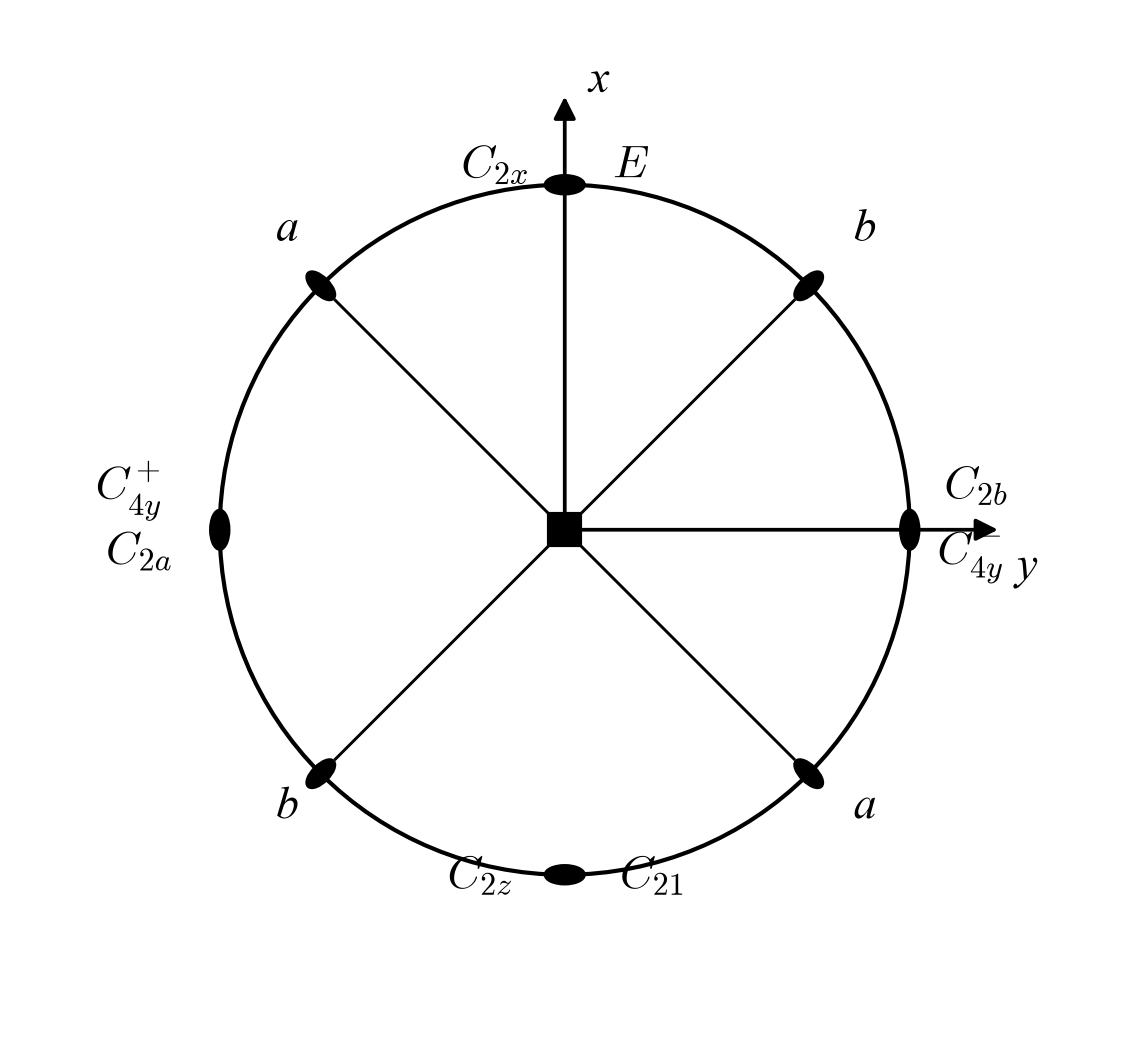
\includegraphics[width=0.60\textwidth]{fig1_1.png}
\caption{三斜、单斜、正交和四方晶系的对称元素。这些晶系中的点群都是 $m3m$（$O_{h}$）的子群，故采用相同记号。$x$、$y$、$z$ 构成右手系。各对称操作的记号标在图中该操作把字母 $E$ 移到的位置上。}
\end{figure}

\begin{figure}[H]
\centering
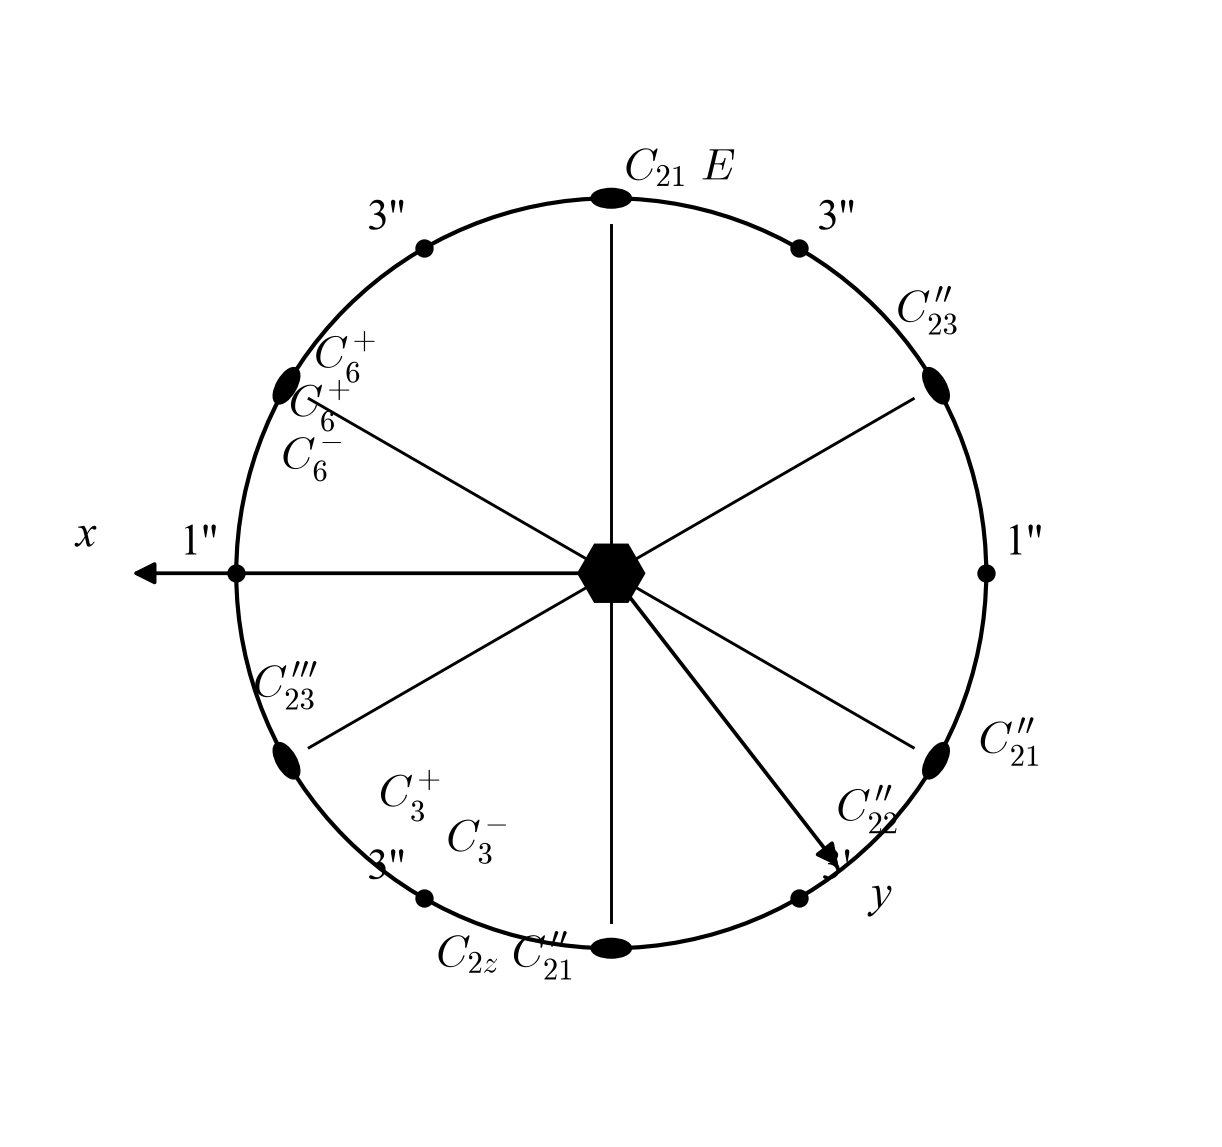
\includegraphics[width=0.62\textwidth]{fig1_2.png}
\caption{三方和六方晶系的对称元素。$z$ 轴垂直于纸面向上。各对称操作的记号标在图中该操作把字母 $E$ 移到的位置上。}
\end{figure}

许多结果的有用性依赖于对称元素的完整辨认，因此我们对此略加讨论。对属于大多数晶系的点群，可以用极射赤面投影图（stereogram）之类的平面图来辨认对称元素：图 1.1 用于三斜、单斜、正交和四方晶系，图 1.2 用于三方和六方晶系。Schiff（1954）曾用双面纸模型帮助想象各种非立方点群。而对立方晶系，直接从立方体图形辨认对称元素更容易，见图 1.3。$C_{nr}^{+}$ 表示把空间的点绕图中标记为 $r$ 的轴逆时针转 $2\pi/n$ 弧度的操作，$C_{nr}^{-}$ 表示绕同一轴顺时针转 $2\pi/n$ 弧度的操作；$E$ 是恒等操作，$I$ 是反演。表 1.2 按七个晶系统一列出了各晶系中出现的算符；表的每一部分分两列，右列元素是左列相应元素与 $I$ 的乘积。表中给出的是相应点群处于相对图的 $x$、$y$、$z$ 轴的标准定向时的元素。某些点群有时必须使用非标准定向，但由于每个元素都有确定的标记，这不会引起混淆。应当注意：反射面一律记作 $\sigma$，其他转动反射记作 $S$；还应指出，在我们采用的记号里 $IC_{2} = \sigma$、$IC_{3}^{+} = S_{6}^{-}$、$IC_{4}^{+} = S_{4}^{-}$、$IC_{6}^{+} = S_{3}^{-}$（即 $IC_{3}^{+} = S_{6}^{-}$，等等）。这是因为 $S_{n}^{+}$ 表示绕轴逆时针转 $2\pi/n$ 后再在垂直于该轴的平面内反射，于是 $IC_{n}^{+} = \sigma C_{2}C_{n}^{+} = \sigma(C_{n}^{+})^{n+2} = (S_{2n}^{-})^{n+2}$。

还有一个重要的、前面已经提过的要点必须强调：处理点群算符时，我们始终把它理解为\textit{主动}算符——移动空间的点而保持坐标轴不动；同样，写成 $\{R \,|\, \mathbf{v}\}$ 形式的空间群算符（见 1.5 节）也按主动算符解释。

\begin{figure}[H]
\centering
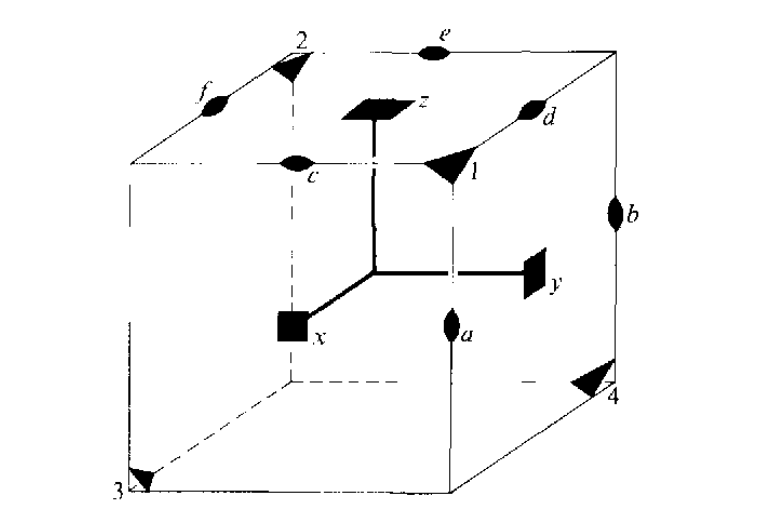
\includegraphics[width=0.58\textwidth]{fig1_3_scan.png}
\caption{立方晶系的对称元素（Altmann and Bradley 1963\textsuperscript{b}）。}
\end{figure}

表 1.3 给出 32 个晶体学点群各自包含的对称操作。点群按七个晶系排列，每个点群的全部元素都已列出。只要点群有主轴，主轴就取在 $Oz$ 方向，这称为\textit{标准定向}（standard setting）；当然还可能有许多其他定向。图 1.4 给出 32 个晶体学点群的极射赤面投影图；投影理论可参见例如 Phillips (1963)。在同一晶系中，含有最多对称操作的点群称为该晶系的\textit{全对称点群}（holosymmetric point group）。

\textit{点群操作的乘法}

对立方群以外的所有点群，借助于极射赤面投影图容易得到两个点群操作相继作用的结果。例如乘法 $C_{2x}C_{4z}^{+} = C_{2b}$ 见图 1.5：图中黑点表示纸面上方的点，圆圈表示纸面下方的点。点 $A$ 经操作 $C_{4z}^{-}$ 变为点 $B$；$B$ 再经操作 $C_{2x}$ 变为点 $C$。总的效果是把 $A$ 直接变为 $C$ 的操作，即 $C_{2b}$，这从图 1.1 可以看出。

\setcounter{figure}{4}
\begin{figure}[H]
\centering
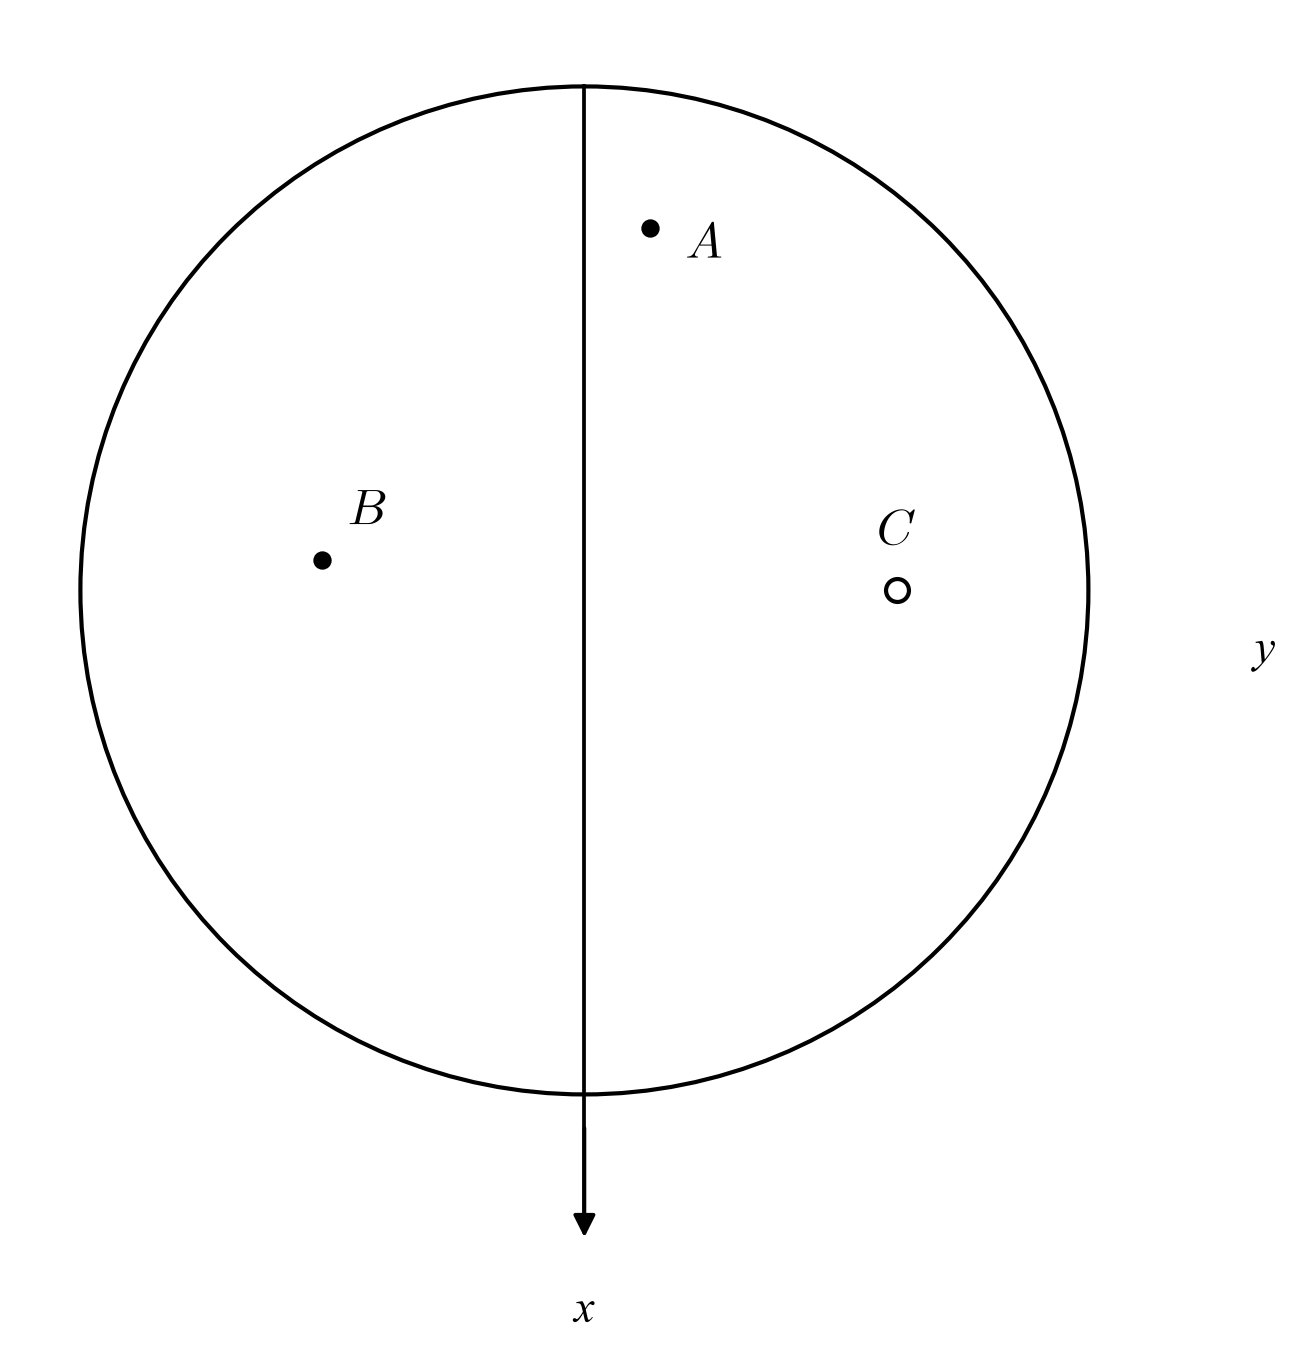
\includegraphics[width=0.55\textwidth]{fig1_5.png}
\caption{点 $A$ 经 $C_{4z}^{-}$ 到 $B$、再经 $C_{2x}$ 到 $C$ 的示意（原书本图无图注文字）。}
\end{figure}

对立方点群，得到群乘法表的最容易方法是使用表 1.4(a) 给出的算符的 Jones 忠实表示符号（Jones' faithful representation symbols）。算符 $R$ 的 Jones 符号就是 $R$ 作用在向量 $(x, y, z)$ 上得到的向量；这些符号正是《X 射线晶体学国际表》第一卷表 4.3 中点式立方与六方空间群的一般等价位置坐标（Henry and Lonsdale 1965）。若 $(x, y, z)$ 是相对沿坐标轴的单位矢量 $\mathbf{i}$、$\mathbf{j}$、$\mathbf{k}$ 给出的，则例如 $C_{4z}^{+}x\mathbf{i} = x\mathbf{j}$，$C_{4z}^{+}y\mathbf{j} = -y\mathbf{i}$，$C_{4z}^{+}z\mathbf{k} = z\mathbf{k}$，于是可写 $C_{4z}^{+}(x, y, z) = (-y, x, z)$，即

\begin{equation*}
C_{4z}^{+}(x\mathbf{i} + y\mathbf{j} + z\mathbf{k}) = (-y\mathbf{i} + x\mathbf{j} + z\mathbf{k})
\tag{1.4.8}
\end{equation*}

因此 $C_{4z}^{+}$ 的 Jones 符号写作 $(\bar{y}xz)$。以行向量 $\langle \mathbf{i}, \mathbf{j}, \mathbf{k}|$ 为基时代表 $C_{4z}^{+}$ 的矩阵是

\begin{equation*}
\mathbf{D}(C_{4z}^{+}) = \begin{pmatrix} 0 & -1 & 0 \\ 1 & 0 & 0 \\ 0 & 0 & 1 \end{pmatrix}
\tag{1.4.9}
\end{equation*}

从而 Jones 符号就是这个矩阵表示的缩写。式 (1.4.9) 来自

\begin{equation*}
C_{4z}^{+}\langle \mathbf{i}, \mathbf{j}, \mathbf{k}| = \langle \mathbf{i}, \mathbf{j}, \mathbf{k}| \begin{pmatrix} 0 & -1 & 0 \\ 1 & 0 & 0 \\ 0 & 0 & 1 \end{pmatrix},
\tag{1.4.10}
\end{equation*}

这说明了 $D$ 为什么是忠实表示。这些符号的乘法规则容易由矩阵乘法导出，例如

\begin{equation*}
(zxy)(\bar{y}xz) = \begin{pmatrix} 0 & 0 & 1 \\ 1 & 0 & 0 \\ 0 & 1 & 0 \end{pmatrix} \begin{pmatrix} 0 & -1 & 0 \\ 1 & 0 & 0 \\ 0 & 0 & 1 \end{pmatrix} = \begin{pmatrix} 0 & 0 & 1 \\ 0 & -1 & 0 \\ 1 & 0 & 0 \end{pmatrix} = (z\bar{y}x).
\tag{1.4.11}
\end{equation*}

其实不必写出完整矩阵：$(zxy)(\bar{y}xz) = (z'x'y')$，其中 $(x'y'z') = (\bar{y}xz)$，于是 $(z'x'y') = (z\bar{y}x)$。式 (1.4.11) 作为表示等式读作

\begin{equation*}
\mathbf{D}(C_{31}^{+})\mathbf{D}(C_{4z}^{+}) = \mathbf{D}(C_{2c})
\tag{1.4.12}
\end{equation*}

这可由表 1.4(a) 看出：表中给出了全部 48 个立方点群操作的 Jones 忠实表示符号。由于 $D$ 是忠实表示，立即可得 $C_{31}^{+}C_{4z}^{+} = C_{2c}$。表 1.4(a) 的 Jones 符号也可用于四方、正交点群的元素，以及单斜、三斜点群的元素——只要向量 $(x, y, z)$ 相对于平行于晶体坐标轴的单位矢量 $\mathbf{i}$、$\mathbf{j}$、$\mathbf{k}$ 给出。表 1.4(b) 中类似的一组符号给出六方或三方点群的操作对向量 $(x, y, z)$ 的作用，此时 $(x, y, z)$ 相对于单位矢量 $\mathbf{i}$、$\mathbf{j}$、$\mathbf{k}$ 给出，而 $\mathbf{i}$ 与 $\mathbf{j}$ 互成 120° 且都在垂直于 $\mathbf{k}$ 的平面内。

表 1.5 与表 1.6 给出点群 432（$O$）与 622（$D_{6}$）的群乘法表（Belov 1957\textsuperscript{b}，Belov and Tarkhova 1960，Hurley 1966，Koptsik 1966）。这两个点群只含纯转动；其余只含纯转动的点群都是这两个点群之一的子群。而每个含有非纯转动操作的点群，都与某个纯转动点群简单地相关联。因此，由表 1.5 与 1.6 可以很快得到 32 个点群中任何一个的群乘法表。

\begin{table}[H]
\centering
\textbf{表 1.2}\quad \textit{七个晶系的对称元素}

\medskip
\resizebox{\textwidth}{!}{%
\begin{tabular}{|c|c|c|c|c|c|c|}
\hline
三斜 & 单斜 & 正交 & 四方 & 三方 & 六方 & 立方 \\ \hline
$\bar{1}$（$C_{i}$） & $2/m$（$C_{2h}$） & $mmm$（$D_{2h}$） & $4/mmm$（$D_{4h}$） & $\bar{3}m$（$D_{3d}$） & $6/mmm$（$D_{6h}$） & $m3m$（$O_{h}$） \\ \hline
$E, I$ & $E, I$ & $E, I$ & $E, I$ & $E, I$ & $E, I$ & $E, I$ \\
 & $C_{2z}, \sigma_{z}$ & $C_{2m}, \sigma_{m}$ & $C_{4z}^{\pm}, S_{4z}^{\mp}$ & $C_{3}^{\pm}, S_{6}^{\mp}$ & $C_{6}^{\pm}, S_{3}^{\mp}$ & $C_{2m}, \sigma_{m}$ \\
 &  &  & $C_{2m}, \sigma_{m}$ & $C'_{2i}, \sigma_{di}$ & $C_{3}^{\pm}, S_{6}^{\mp}$ & $C_{3j}^{\pm}, S_{6j}^{\mp}$ \\
 &  &  & $C_{2s}, \sigma_{ds}$ &  & $C_{2}, \sigma_{h}$ & $C_{4m}^{\pm}, S_{4m}^{\mp}$ \\
 &  &  &  &  & $C'_{2i}, \sigma_{di}$ & $C_{2p}, \sigma_{dp}$ \\
 &  &  &  &  & $C''_{2i}, \sigma_{vi}$ &  \\ \hline
\end{tabular}}

\smallskip
\parbox{0.92\textwidth}{\textit{表 1.2 的注.}
(i) 三方晶系还有一种定向，以 $C''_{2i}$ 代替 $C'_{2i}$ 作为标准定向。
(ii) 下列轴的位置见图 1.1、1.2、1.3：$m = x, y, z$；$s = a, b$；$i = 1, 2, 3$；$j = 1, 2, 3, 4$；$p = a, b, c, d, e, f$。}
\end{table}

\begin{table}[H]
\centering
\textbf{表 1.3}\quad \textit{32 个点群}

\smallskip
\begin{tabular}{|c|c|c|p{0.58\textwidth}|}
\hline
编号 & 国际记号 & Schönflies 记号 & 元素 \\ \hline
\multicolumn{4}{|l|}{\textit{三斜}} \\ \hline
1 & $1$ & $C_{1}$ & $E$ \\ \hline
2 & $\bar{1}$ & $C_{i}$ & $E$, $I$ \\ \hline
\multicolumn{4}{|l|}{\textit{单斜}} \\ \hline
3 & $2$ & $C_{2}$ & $E$, $C_{2z}$ \\ \hline
4 & $m$ & $C_{s}$, $C_{1h}$ & $E$, $\sigma_{z}$ \\ \hline
5 & $2/m$ & $C_{2h}$ & $E$, $C_{2z}$, $I$, $\sigma_{z}$ \\ \hline
\multicolumn{4}{|l|}{\textit{正交}} \\ \hline
6 & $222$ & $D_{2}$ & $E$, $C_{2x}$, $C_{2y}$, $C_{2z}$ \\ \hline
7 & $mm2$ & $C_{2v}$ & $E$, $C_{2z}$, $\sigma_{x}$, $\sigma_{y}$ \\ \hline
8 & $mmm$ & $D_{2h}$ & $E$, $C_{2x}$, $C_{2y}$, $C_{2z}$, $I$, $\sigma_{x}$, $\sigma_{y}$, $\sigma_{z}$ \\ \hline
\multicolumn{4}{|l|}{\textit{四方}} \\ \hline
9 & $4$ & $C_{4}$ & $E$, $C_{4z}^{+}$, $C_{4z}^{-}$, $C_{2z}$ \\ \hline
10 & $\bar{4}$ & $S_{4}$ & $E$, $S_{4z}^{+}$, $S_{4z}^{-}$, $C_{2z}$ \\ \hline
11 & $4/m$ & $C_{4h}$ & $E$, $C_{4z}^{+}$, $C_{4z}^{-}$, $C_{2z}$, $I$, $S_{4z}^{-}$, $S_{4z}^{+}$, $\sigma_{z}$ \\ \hline
12 & $422$ & $D_{4}$ & $E$, $C_{4z}^{+}$, $C_{4z}^{-}$, $C_{2z}$, $C_{2x}$, $C_{2y}$, $C_{2a}$, $C_{2b}$ \\ \hline
13 & $4mm$ & $C_{4v}$ & $E$, $C_{4z}^{+}$, $C_{4z}^{-}$, $C_{2z}$, $\sigma_{x}$, $\sigma_{y}$, $\sigma_{da}$, $\sigma_{db}$ \\ \hline
14 & $\bar{4}2m$ & $D_{2d}$ & $E$, $S_{4z}^{+}$, $S_{4z}^{-}$, $C_{2z}$, $C_{2x}$, $C_{2y}$, $\sigma_{da}$, $\sigma_{db}$ \\ \hline
15 & $4/mmm$ & $D_{4h}$ & $E$, $C_{4z}^{+}$, $C_{4z}^{-}$, $C_{2z}$, $C_{2x}$, $C_{2y}$, $C_{2a}$, $C_{2b}$, $I$, $S_{4z}^{-}$, $S_{4z}^{+}$, $\sigma_{z}$, $\sigma_{x}$, $\sigma_{y}$, $\sigma_{da}$, $\sigma_{db}$ \\ \hline
\multicolumn{4}{|l|}{\textit{三方}} \\ \hline
16 & $3$ & $C_{3}$ & $E$, $C_{3}^{+}$, $C_{3}^{-}$ \\ \hline
17 & $\bar{3}$ & $C_{3i}$ & $E$, $C_{3}^{+}$, $C_{3}^{-}$, $I$, $S_{6}^{-}$, $S_{6}^{+}$ \\ \hline
18 & $32$ & $D_{3}$ & $E$, $C_{3}^{+}$, $C_{3}^{-}$, $C'_{21}$, $C'_{22}$, $C'_{23}$ \\ \hline
19 & $3m$ & $C_{3v}$ & $E$, $C_{3}^{+}$, $C_{3}^{-}$, $\sigma_{d1}$, $\sigma_{d2}$, $\sigma_{d3}$ \\ \hline
20 & $\bar{3}m$ & $D_{3d}$ & $E$, $C_{3}^{+}$, $C_{3}^{-}$, $C'_{21}$, $C'_{22}$, $C'_{23}$, $I$, $S_{6}^{-}$, $S_{6}^{+}$, $\sigma_{d1}$, $\sigma_{d2}$, $\sigma_{d3}$ \\ \hline
\multicolumn{4}{|l|}{\textit{六方}} \\ \hline
21 & $6$ & $C_{6}$ & $E$, $C_{6}^{+}$, $C_{6}^{-}$, $C_{3}^{+}$, $C_{3}^{-}$, $C_{2}$ \\ \hline
22 & $\bar{6}$ & $C_{3h}$ & $E$, $S_{3}^{-}$, $S_{3}^{+}$, $C_{3}^{+}$, $C_{3}^{-}$, $\sigma_{h}$ \\ \hline
23 & $6/m$ & $C_{6h}$ & $E$, $C_{6}^{+}$, $C_{6}^{-}$, $C_{3}^{+}$, $C_{3}^{-}$, $C_{2}$, $I$, $S_{3}^{-}$, $S_{3}^{+}$, $S_{6}^{-}$, $S_{6}^{+}$, $\sigma_{h}$ \\ \hline
24 & $622$ & $D_{6}$ & $E$, $C_{6}^{+}$, $C_{6}^{-}$, $C_{3}^{+}$, $C_{3}^{-}$, $C_{2}$, $C'_{21}$, $C'_{22}$, $C'_{23}$, $C''_{21}$, $C''_{22}$, $C''_{23}$ \\ \hline
25 & $6mm$ & $C_{6v}$ & $E$, $C_{6}^{+}$, $C_{6}^{-}$, $C_{3}^{+}$, $C_{3}^{-}$, $C_{2}$, $\sigma_{d1}$, $\sigma_{d2}$, $\sigma_{d3}$, $\sigma_{v1}$, $\sigma_{v2}$, $\sigma_{v3}$ \\ \hline
26 & $\bar{6}2m$ & $D_{3h}$ & $E$, $S_{3}^{-}$, $S_{3}^{+}$, $C_{3}^{+}$, $C_{3}^{-}$, $\sigma_{h}$, $C'_{21}$, $C'_{22}$, $C'_{23}$, $\sigma_{v1}$, $\sigma_{v2}$, $\sigma_{v3}$ \\ \hline
27 & $6/mmm$ & $D_{6h}$ & $E$, $C_{6}^{+}$, $C_{6}^{-}$, $C_{3}^{+}$, $C_{3}^{-}$, $C_{2}$, $C'_{21}$, $C'_{22}$, $C'_{23}$, $C''_{21}$, $C''_{22}$, $C''_{23}$, $I$, $S_{3}^{-}$, $S_{3}^{+}$, $S_{6}^{-}$, $S_{6}^{+}$, $\sigma_{h}$, $\sigma_{d1}$, $\sigma_{d2}$, $\sigma_{d3}$, $\sigma_{v1}$, $\sigma_{v2}$, $\sigma_{v3}$ \\ \hline
\multicolumn{4}{|l|}{\textit{立方}} \\ \hline
28 & $23$ & $T$ & $E$, $C_{2m}$, $C_{3j}^{+}$, $C_{3j}^{-}$ \\ \hline
29 & $m3$ & $T_{h}$ & $E$, $C_{2m}$, $C_{3j}^{+}$, $C_{3j}^{-}$, $I$, $\sigma_{m}$, $S_{6j}^{-}$, $S_{6j}^{+}$ \\ \hline
30 & $432$ & $O$ & $E$, $C_{2m}$, $C_{3j}^{+}$, $C_{3j}^{-}$, $C_{2p}$, $C_{4m}^{+}$, $C_{4m}^{-}$ \\ \hline
31 & $\bar{4}3m$ & $T_{d}$ & $E$, $C_{2m}$, $C_{3j}^{+}$, $C_{3j}^{-}$, $\sigma_{dp}$, $S_{4m}^{-}$, $S_{4m}^{+}$ \\ \hline
32 & $m3m$ & $O_{h}$ & $E$, $C_{2m}$, $C_{3j}^{+}$, $C_{3j}^{-}$, $C_{2p}$, $C_{4m}^{+}$, $C_{4m}^{-}$, $I$, $\sigma_{m}$, $S_{6j}^{-}$, $S_{6j}^{+}$, $\sigma_{dp}$, $S_{4m}^{-}$, $S_{4m}^{+}$ \\ \hline
\end{tabular}

\end{table}

\noindent\textit{表 1.3 的注.}\ （i）第 1 列的编号是任意的，采用 Koster, Dimmock, Wheeler, and Statz (1963) 的编号。（ii）对称操作的标记可由图 1.1--1.3 辨认：$j = 1, 2, 3, 4$；$m = x, y, z$；$p = a, b, c, d, e, f$。（iii）主轴已取在 $Oz$ 方向，但某些点群仍可能有其他定向，例如 $\bar{4}2m$（$D_{2d}$）也可以包含元素 $E$、$S_{4z}^{-}$、$C_{2z}$、$S_{4z}^{+}$、$\sigma_{x}$、$\sigma_{y}$、$C_{2a}$ 与 $C_{2b}$；在考虑空间群（见第 3 章）时这类不同的取法有时很重要。

\setcounter{figure}{3}
\begin{figure}[H]
\centering
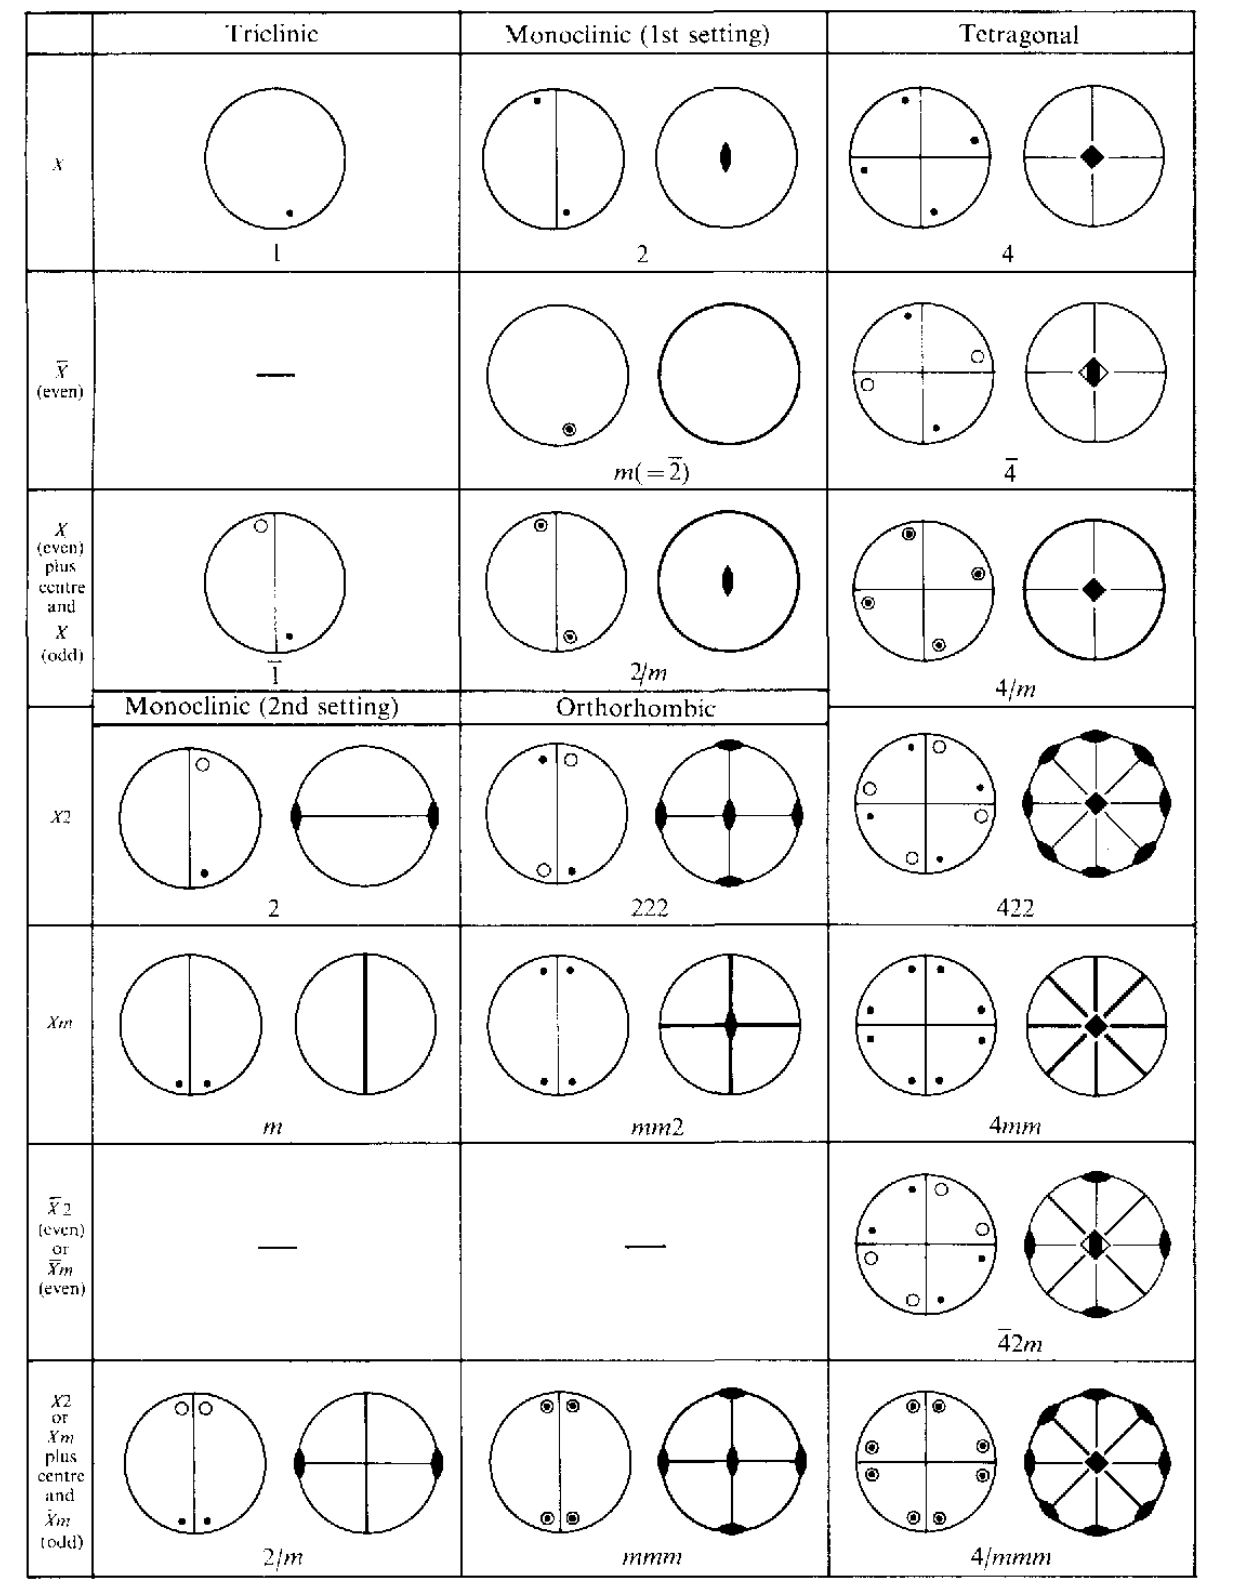
\includegraphics[width=0.88\textwidth]{fig1_4a_scan.png}
\end{figure}
\clearpage
\begin{figure}[H]
\centering
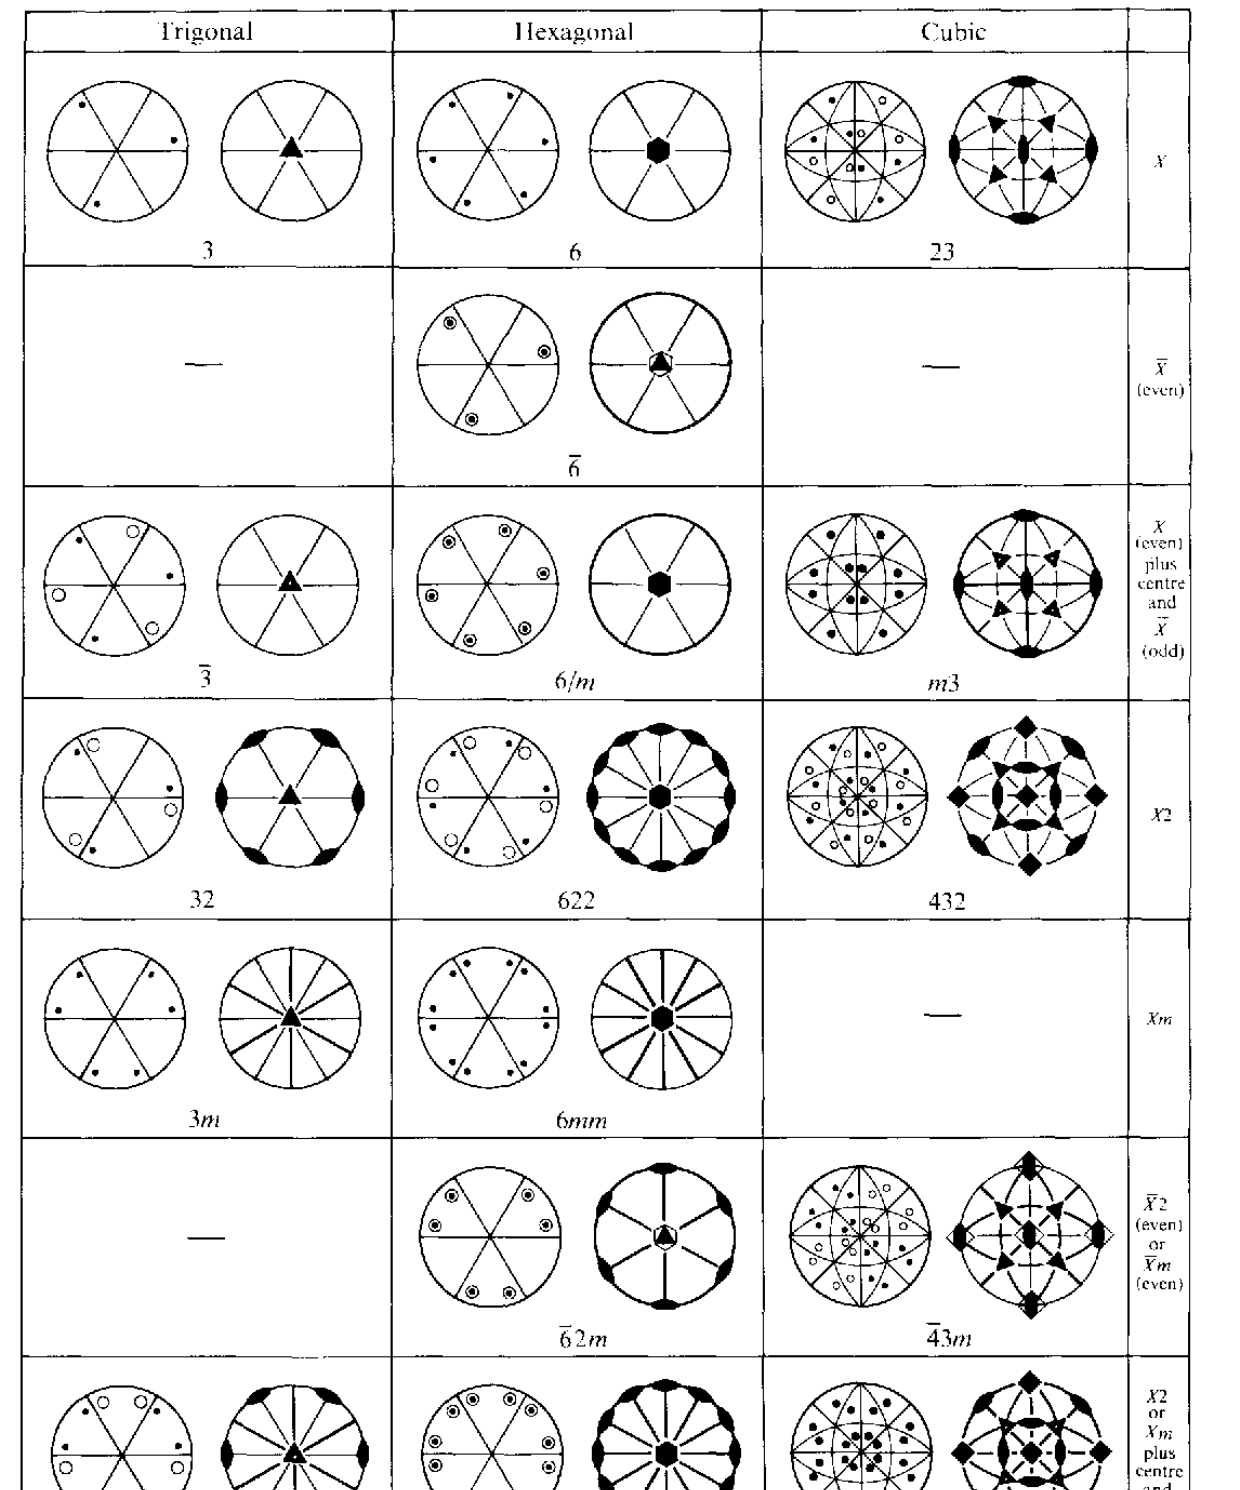
\includegraphics[width=0.88\textwidth]{fig1_4b_scan.png}
\caption{32 个点群的一般等价方向极点的极射赤面投影图及各点群的对称元素（所有图中 $z$ 轴均垂直于纸面；$m3$ 与 $m3m$ 只画出一半的点）（Henry and Lonsdale 1965）。列：三斜、单斜（第一种定向）、四方、三方、六方、立方，以及单斜（第二种定向）与正交；行：$\chi$；$\bar{\chi}$（偶）；$\chi$（偶）加对称中心与 $\chi$（奇）；$\chi 2$；$\chi m$；$\bar{\chi}2$（偶）或 $\bar{\chi}m$（偶）；$\chi 2$ 或 $\chi m$ 加对称中心与 $\chi m$（奇）。}
\end{figure}
\setcounter{figure}{5}

% 1.5 空间群
\section{空间群}

在讨论空间群的定义之前，先要说明什么是\textit{布拉维格子}。格子是数学点的集合，其中每个格点的环境在相同取向下完全相同。就晶体而言，构成晶体的原子或分子按规则方式排列（Haüy 1815\textsuperscript{a}–\textsuperscript{d}）；也就是说，晶体内部存在一组数学格点。如果让一位麦克斯韦妖从这个格点组中的任意一点观察晶体，他看到的原子或分子的排布与从其他任何格点看到的完全相同。严格地说，要使每个格点的环境完全相似，数学格子必须是无穷延伸的；真实晶体显然不可能包含这样的无穷格子，但考虑到原子的实际尺寸，它非常接近于无穷格子。我们可以用二维例子来说明格子的概念：图 1.6 中那组按特定方式排列、并被想象为延伸到图外无穷远的点，就构成正方二维布拉维格子 $p$。

\textbf{表 1.5}\quad \textit{点群 432（$O$）的群乘法表}

\noindent\resizebox{\textwidth}{!}{%
\begin{tabular}{|c||c||c||c||c||c||c||c||c||c||c||c||c||c||c||c||c||c||c||c||c||c||c||c||c|}
\hline
 & $E$ & $C_{2x}$ & $C_{2y}$ & $C_{2z}$ & $C_{4x}^{-}$ & $C_{4y}^{-}$ & $C_{4z}^{-}$ & $C_{4x}^{+}$ & $C_{4y}^{+}$ & $C_{4z}^{+}$ & $C_{31}^{-}$ & $C_{32}^{-}$ & $C_{33}^{-}$ & $C_{34}^{-}$ & $C_{31}^{+}$ & $C_{32}^{+}$ & $C_{33}^{+}$ & $C_{34}^{+}$ & $C_{2a}$ & $C_{2b}$ & $C_{2c}$ & $C_{2d}$ & $C_{2e}$ & $C_{2f}$ \\ \hline
$E$ & $E$ & $C_{2x}$ & $C_{2y}$ & $C_{2z}$ & $C_{4x}^{-}$ & $C_{4y}^{-}$ & $C_{4z}^{-}$ & $C_{4x}^{+}$ & $C_{4y}^{+}$ & $C_{4z}^{+}$ & $C_{31}^{-}$ & $C_{32}^{-}$ & $C_{33}^{-}$ & $C_{34}^{-}$ & $C_{31}^{+}$ & $C_{32}^{+}$ & $C_{33}^{+}$ & $C_{34}^{+}$ & $C_{2a}$ & $C_{2b}$ & $C_{2c}$ & $C_{2d}$ & $C_{2e}$ & $C_{2f}$ \\ \hline
$C_{2x}$ & $C_{2x}$ & $E$ & $C_{2z}$ & $C_{2y}$ & $C_{4x}^{+}$ & $C_{2d}$ & $C_{2a}$ & $C_{4x}^{-}$ & $C_{2c}$ & $C_{2b}$ & $C_{32}^{-}$ & $C_{31}^{-}$ & $C_{34}^{-}$ & $C_{33}^{-}$ & $C_{34}^{+}$ & $C_{33}^{+}$ & $C_{32}^{+}$ & $C_{31}^{+}$ & $C_{4z}^{-}$ & $C_{4z}^{+}$ & $C_{4y}^{+}$ & $C_{4y}^{-}$ & $C_{2f}$ & $C_{2e}$ \\ \hline
$C_{2y}$ & $C_{2y}$ & $C_{2z}$ & $E$ & $C_{2x}$ & $C_{2e}$ & $C_{4y}^{+}$ & $C_{2b}$ & $C_{2f}$ & $C_{4y}^{-}$ & $C_{2a}$ & $C_{33}^{-}$ & $C_{34}^{-}$ & $C_{31}^{-}$ & $C_{32}^{-}$ & $C_{32}^{+}$ & $C_{31}^{+}$ & $C_{34}^{+}$ & $C_{33}^{+}$ & $C_{4z}^{+}$ & $C_{4z}^{-}$ & $C_{2d}$ & $C_{2c}$ & $C_{4x}^{-}$ & $C_{4x}^{+}$ \\ \hline
$C_{2z}$ & $C_{2z}$ & $C_{2y}$ & $C_{2x}$ & $E$ & $C_{2f}$ & $C_{2c}$ & $C_{4z}^{+}$ & $C_{2e}$ & $C_{2d}$ & $C_{4z}^{-}$ & $C_{34}^{-}$ & $C_{33}^{-}$ & $C_{32}^{-}$ & $C_{31}^{-}$ & $C_{33}^{+}$ & $C_{34}^{+}$ & $C_{31}^{+}$ & $C_{32}^{+}$ & $C_{2b}$ & $C_{2a}$ & $C_{4y}^{-}$ & $C_{4y}^{+}$ & $C_{4x}^{+}$ & $C_{4x}^{-}$ \\ \hline
$C_{4x}^{-}$ & $C_{4x}^{-}$ & $C_{4x}^{+}$ & $C_{2f}$ & $C_{2e}$ & $C_{2x}$ & $C_{32}^{+}$ & $C_{31}^{-}$ & $E$ & $C_{34}^{+}$ & $C_{33}^{-}$ & $C_{2a}$ & $C_{4z}^{-}$ & $C_{2b}$ & $C_{4z}^{+}$ & $C_{4y}^{+}$ & $C_{2d}$ & $C_{4y}^{-}$ & $C_{2c}$ & $C_{32}^{-}$ & $C_{34}^{-}$ & $C_{31}^{+}$ & $C_{33}^{+}$ & $C_{2y}$ & $C_{2z}$ \\ \hline
$C_{4y}^{-}$ & $C_{4y}^{-}$ & $C_{2c}$ & $C_{4y}^{+}$ & $C_{2d}$ & $C_{31}^{-}$ & $C_{2y}$ & $C_{33}^{+}$ & $C_{34}^{-}$ & $E$ & $C_{32}^{+}$ & $C_{2e}$ & $C_{4x}^{+}$ & $C_{4x}^{-}$ & $C_{2f}$ & $C_{4z}^{+}$ & $C_{2a}$ & $C_{2b}$ & $C_{4z}^{-}$ & $C_{31}^{+}$ & $C_{34}^{+}$ & $C_{2z}$ & $C_{2x}$ & $C_{33}^{-}$ & $C_{32}^{-}$ \\ \hline
$C_{4z}^{-}$ & $C_{4z}^{-}$ & $C_{2b}$ & $C_{2a}$ & $C_{4z}^{+}$ & $C_{34}^{+}$ & $C_{31}^{-}$ & $C_{2z}$ & $C_{33}^{+}$ & $C_{32}^{-}$ & $E$ & $C_{2c}$ & $C_{2d}$ & $C_{4y}^{+}$ & $C_{4y}^{-}$ & $C_{4x}^{+}$ & $C_{4x}^{-}$ & $C_{2e}$ & $C_{2f}$ & $C_{2x}$ & $C_{2y}$ & $C_{34}^{-}$ & $C_{33}^{-}$ & $C_{31}^{+}$ & $C_{32}^{+}$ \\ \hline
$C_{4x}^{+}$ & $C_{4x}^{+}$ & $C_{4x}^{-}$ & $C_{2e}$ & $C_{2f}$ & $E$ & $C_{33}^{+}$ & $C_{32}^{-}$ & $C_{2x}$ & $C_{31}^{+}$ & $C_{34}^{-}$ & $C_{4z}^{-}$ & $C_{2a}$ & $C_{4z}^{+}$ & $C_{2b}$ & $C_{2c}$ & $C_{4y}^{-}$ & $C_{2d}$ & $C_{4y}^{+}$ & $C_{31}^{-}$ & $C_{33}^{-}$ & $C_{34}^{+}$ & $C_{32}^{+}$ & $C_{2z}$ & $C_{2y}$ \\ \hline
$C_{4y}^{+}$ & $C_{4y}^{+}$ & $C_{2d}$ & $C_{4y}^{-}$ & $C_{2c}$ & $C_{33}^{-}$ & $E$ & $C_{34}^{+}$ & $C_{32}^{-}$ & $C_{2y}$ & $C_{31}^{+}$ & $C_{4x}^{-}$ & $C_{2f}$ & $C_{2e}$ & $C_{4x}^{+}$ & $C_{2a}$ & $C_{4z}^{+}$ & $C_{4z}^{-}$ & $C_{2b}$ & $C_{32}^{+}$ & $C_{33}^{+}$ & $C_{2x}$ & $C_{2z}$ & $C_{31}^{-}$ & $C_{34}^{-}$ \\ \hline
$C_{4z}^{+}$ & $C_{4z}^{+}$ & $C_{2a}$ & $C_{2b}$ & $C_{4z}^{-}$ & $C_{32}^{+}$ & $C_{34}^{-}$ & $E$ & $C_{31}^{+}$ & $C_{33}^{-}$ & $C_{2z}$ & $C_{4y}^{-}$ & $C_{4y}^{+}$ & $C_{2d}$ & $C_{2c}$ & $C_{2e}$ & $C_{2f}$ & $C_{4x}^{+}$ & $C_{4x}^{-}$ & $C_{2y}$ & $C_{2x}$ & $C_{31}^{-}$ & $C_{32}^{-}$ & $C_{33}^{+}$ & $C_{34}^{+}$ \\ \hline
$C_{31}^{-}$ & $C_{31}^{-}$ & $C_{34}^{-}$ & $C_{32}^{-}$ & $C_{33}^{-}$ & $C_{2c}$ & $C_{2a}$ & $C_{2e}$ & $C_{4y}^{-}$ & $C_{4z}^{-}$ & $C_{4x}^{-}$ & $C_{31}^{+}$ & $C_{33}^{+}$ & $C_{34}^{+}$ & $C_{32}^{+}$ & $E$ & $C_{2x}$ & $C_{2y}$ & $C_{2z}$ & $C_{4x}^{+}$ & $C_{2f}$ & $C_{4z}^{+}$ & $C_{2b}$ & $C_{4y}^{+}$ & $C_{2d}$ \\ \hline
$C_{32}^{-}$ & $C_{32}^{-}$ & $C_{33}^{-}$ & $C_{31}^{-}$ & $C_{34}^{-}$ & $C_{4y}^{+}$ & $C_{4z}^{-}$ & $C_{2f}$ & $C_{2d}$ & $C_{2a}$ & $C_{4x}^{+}$ & $C_{34}^{+}$ & $C_{32}^{+}$ & $C_{31}^{+}$ & $C_{33}^{+}$ & $C_{2x}$ & $E$ & $C_{2z}$ & $C_{2y}$ & $C_{4x}^{-}$ & $C_{2e}$ & $C_{2b}$ & $C_{4z}^{+}$ & $C_{2c}$ & $C_{4y}^{-}$ \\ \hline
$C_{33}^{-}$ & $C_{33}^{-}$ & $C_{32}^{-}$ & $C_{34}^{-}$ & $C_{31}^{-}$ & $C_{2d}$ & $C_{4z}^{+}$ & $C_{4x}^{-}$ & $C_{4y}^{+}$ & $C_{2b}$ & $C_{2e}$ & $C_{32}^{+}$ & $C_{34}^{+}$ & $C_{33}^{+}$ & $C_{31}^{+}$ & $C_{2y}$ & $C_{2z}$ & $E$ & $C_{2x}$ & $C_{2f}$ & $C_{4x}^{+}$ & $C_{2a}$ & $C_{4z}^{-}$ & $C_{4y}^{-}$ & $C_{2c}$ \\ \hline
$C_{34}^{-}$ & $C_{34}^{-}$ & $C_{31}^{-}$ & $C_{33}^{-}$ & $C_{32}^{-}$ & $C_{4y}^{-}$ & $C_{2b}$ & $C_{4x}^{+}$ & $C_{2c}$ & $C_{4z}^{+}$ & $C_{2f}$ & $C_{33}^{+}$ & $C_{31}^{+}$ & $C_{32}^{+}$ & $C_{34}^{+}$ & $C_{2z}$ & $C_{2y}$ & $C_{2x}$ & $E$ & $C_{2e}$ & $C_{4x}^{-}$ & $C_{4z}^{-}$ & $C_{2a}$ & $C_{2d}$ & $C_{4y}^{+}$ \\ \hline
$C_{31}^{+}$ & $C_{31}^{+}$ & $C_{32}^{+}$ & $C_{33}^{+}$ & $C_{34}^{+}$ & $C_{4z}^{+}$ & $C_{4x}^{+}$ & $C_{4y}^{+}$ & $C_{2a}$ & $C_{2e}$ & $C_{2c}$ & $E$ & $C_{2y}$ & $C_{2z}$ & $C_{2x}$ & $C_{31}^{-}$ & $C_{34}^{-}$ & $C_{32}^{-}$ & $C_{33}^{-}$ & $C_{4y}^{-}$ & $C_{2d}$ & $C_{4x}^{-}$ & $C_{2f}$ & $C_{4z}^{-}$ & $C_{2b}$ \\ \hline
$C_{32}^{+}$ & $C_{32}^{+}$ & $C_{31}^{+}$ & $C_{34}^{+}$ & $C_{33}^{+}$ & $C_{2a}$ & $C_{2f}$ & $C_{4y}^{-}$ & $C_{4z}^{+}$ & $C_{4x}^{-}$ & $C_{2d}$ & $C_{2y}$ & $E$ & $C_{2x}$ & $C_{2z}$ & $C_{33}^{-}$ & $C_{32}^{-}$ & $C_{34}^{-}$ & $C_{31}^{-}$ & $C_{4y}^{+}$ & $C_{2c}$ & $C_{2e}$ & $C_{4x}^{+}$ & $C_{2b}$ & $C_{4z}^{-}$ \\ \hline
$C_{33}^{+}$ & $C_{33}^{+}$ & $C_{34}^{+}$ & $C_{31}^{+}$ & $C_{32}^{+}$ & $C_{4z}^{-}$ & $C_{2e}$ & $C_{2d}$ & $C_{2b}$ & $C_{4x}^{+}$ & $C_{4y}^{-}$ & $C_{2z}$ & $C_{2x}$ & $E$ & $C_{2y}$ & $C_{34}^{-}$ & $C_{31}^{-}$ & $C_{33}^{-}$ & $C_{32}^{-}$ & $C_{2c}$ & $C_{4y}^{+}$ & $C_{2f}$ & $C_{4x}^{-}$ & $C_{4z}^{+}$ & $C_{2a}$ \\ \hline
$C_{34}^{+}$ & $C_{34}^{+}$ & $C_{33}^{+}$ & $C_{32}^{+}$ & $C_{31}^{+}$ & $C_{2b}$ & $C_{4x}^{-}$ & $C_{2c}$ & $C_{4z}^{-}$ & $C_{2f}$ & $C_{4y}^{+}$ & $C_{2x}$ & $C_{2z}$ & $C_{2y}$ & $E$ & $C_{32}^{-}$ & $C_{33}^{-}$ & $C_{31}^{-}$ & $C_{34}^{-}$ & $C_{2d}$ & $C_{4y}^{-}$ & $C_{4x}^{+}$ & $C_{2e}$ & $C_{2a}$ & $C_{4z}^{+}$ \\ \hline
$C_{2a}$ & $C_{2a}$ & $C_{4z}^{+}$ & $C_{4z}^{-}$ & $C_{2b}$ & $C_{31}^{+}$ & $C_{32}^{-}$ & $C_{2y}$ & $C_{32}^{+}$ & $C_{31}^{-}$ & $C_{2x}$ & $C_{4y}^{+}$ & $C_{4y}^{-}$ & $C_{2c}$ & $C_{2d}$ & $C_{4x}^{-}$ & $C_{4x}^{+}$ & $C_{2f}$ & $C_{2e}$ & $E$ & $C_{2z}$ & $C_{33}^{-}$ & $C_{34}^{-}$ & $C_{34}^{+}$ & $C_{33}^{+}$ \\ \hline
$C_{2b}$ & $C_{2b}$ & $C_{4z}^{-}$ & $C_{4z}^{+}$ & $C_{2a}$ & $C_{33}^{+}$ & $C_{33}^{-}$ & $C_{2x}$ & $C_{34}^{+}$ & $C_{34}^{-}$ & $C_{2y}$ & $C_{2d}$ & $C_{2c}$ & $C_{4y}^{-}$ & $C_{4y}^{+}$ & $C_{2f}$ & $C_{2e}$ & $C_{4x}^{-}$ & $C_{4x}^{+}$ & $C_{2z}$ & $E$ & $C_{32}^{-}$ & $C_{31}^{-}$ & $C_{32}^{+}$ & $C_{31}^{+}$ \\ \hline
$C_{2c}$ & $C_{2c}$ & $C_{4y}^{-}$ & $C_{2d}$ & $C_{4y}^{+}$ & $C_{34}^{-}$ & $C_{2x}$ & $C_{31}^{+}$ & $C_{31}^{-}$ & $C_{2z}$ & $C_{34}^{+}$ & $C_{4x}^{+}$ & $C_{2e}$ & $C_{2f}$ & $C_{4x}^{-}$ & $C_{4z}^{-}$ & $C_{2b}$ & $C_{2a}$ & $C_{4z}^{+}$ & $C_{33}^{+}$ & $C_{32}^{+}$ & $E$ & $C_{2y}$ & $C_{32}^{-}$ & $C_{33}^{-}$ \\ \hline
$C_{2d}$ & $C_{2d}$ & $C_{4y}^{+}$ & $C_{2c}$ & $C_{4y}^{-}$ & $C_{32}^{-}$ & $C_{2z}$ & $C_{32}^{+}$ & $C_{33}^{-}$ & $C_{2x}$ & $C_{33}^{+}$ & $C_{2f}$ & $C_{4x}^{-}$ & $C_{4x}^{+}$ & $C_{2e}$ & $C_{2b}$ & $C_{4z}^{-}$ & $C_{4z}^{+}$ & $C_{2a}$ & $C_{34}^{+}$ & $C_{31}^{+}$ & $C_{2y}$ & $E$ & $C_{34}^{-}$ & $C_{31}^{-}$ \\ \hline
$C_{2e}$ & $C_{2e}$ & $C_{2f}$ & $C_{4x}^{+}$ & $C_{4x}^{-}$ & $C_{2z}$ & $C_{31}^{+}$ & $C_{33}^{-}$ & $C_{2y}$ & $C_{33}^{+}$ & $C_{31}^{-}$ & $C_{4z}^{+}$ & $C_{2b}$ & $C_{4z}^{-}$ & $C_{2a}$ & $C_{4y}^{-}$ & $C_{2c}$ & $C_{4y}^{+}$ & $C_{2d}$ & $C_{34}^{-}$ & $C_{32}^{-}$ & $C_{32}^{+}$ & $C_{34}^{+}$ & $E$ & $C_{2x}$ \\ \hline
$C_{2f}$ & $C_{2f}$ & $C_{2e}$ & $C_{4x}^{-}$ & $C_{4x}^{+}$ & $C_{2y}$ & $C_{34}^{+}$ & $C_{34}^{-}$ & $C_{2z}$ & $C_{32}^{+}$ & $C_{32}^{-}$ & $C_{2b}$ & $C_{4z}^{+}$ & $C_{2a}$ & $C_{4z}^{-}$ & $C_{2d}$ & $C_{4y}^{+}$ & $C_{2c}$ & $C_{4y}^{-}$ & $C_{33}^{-}$ & $C_{31}^{-}$ & $C_{33}^{+}$ & $C_{31}^{+}$ & $C_{2x}$ & $E$ \\ \hline
\end{tabular}}

\parbox{0.92\textwidth}{
\textit{表 1.5 的注.} 列标题自左至右依次为：$E$；$C_{2x}, C_{2y}, C_{2z}$；$C_{4x}^{-}, C_{4y}^{-}, C_{4z}^{-}, C_{4x}^{+}, C_{4y}^{+}, C_{4z}^{+}$；$C_{31}^{-}, C_{32}^{-}, C_{33}^{-}, C_{34}^{-}, C_{31}^{+}, C_{32}^{+}, C_{33}^{+}, C_{34}^{+}$；$C_{2a}, C_{2b}, C_{2c}, C_{2d}, C_{2e}, C_{2f}$。行标题相同，顺序一致。求乘积 $LM$ 时，取行首元素为 $L$ 的一行与列标题为 $M$ 的一列的交叉格。——中译者
}

\textbf{表 1.6}\quad \textit{点群 622（$D_{6}$）的群乘法表}

\noindent\resizebox{\textwidth}{!}{%
\begin{tabular}{|c||c||c||c||c||c||c||c||c||c||c||c||c|}
\hline
 & $E$ & $C_{6}^{+}$ & $C_{3}^{+}$ & $C_{2}$ & $C_{3}^{-}$ & $C_{6}^{-}$ & $C'_{21}$ & $C'_{22}$ & $C'_{23}$ & $C''_{21}$ & $C''_{22}$ & $C''_{23}$ \\ \hline
$E$ & $E$ & $C_{6}^{+}$ & $C_{3}^{+}$ & $C_{2}$ & $C_{3}^{-}$ & $C_{6}^{-}$ & $C'_{21}$ & $C'_{22}$ & $C'_{23}$ & $C''_{21}$ & $C''_{22}$ & $C''_{23}$ \\ \hline
$C_{6}^{+}$ & $C_{6}^{+}$ & $C_{3}^{+}$ & $C_{2}$ & $C_{3}^{-}$ & $C_{6}^{-}$ & $E$ & $C''_{22}$ & $C''_{23}$ & $C''_{21}$ & $C'_{22}$ & $C'_{23}$ & $C'_{21}$ \\ \hline
$C_{3}^{+}$ & $C_{3}^{+}$ & $C_{2}$ & $C_{3}^{-}$ & $C_{6}^{-}$ & $E$ & $C_{6}^{+}$ & $C'_{23}$ & $C'_{21}$ & $C'_{22}$ & $C''_{23}$ & $C''_{21}$ & $C''_{22}$ \\ \hline
$C_{2}$ & $C_{2}$ & $C_{3}^{-}$ & $C_{6}^{-}$ & $E$ & $C_{6}^{+}$ & $C_{3}^{+}$ & $C''_{21}$ & $C''_{22}$ & $C''_{23}$ & $C'_{21}$ & $C'_{22}$ & $C'_{23}$ \\ \hline
$C_{3}^{-}$ & $C_{3}^{-}$ & $C_{6}^{-}$ & $E$ & $C_{6}^{+}$ & $C_{3}^{+}$ & $C_{2}$ & $C'_{22}$ & $C'_{23}$ & $C'_{21}$ & $C''_{22}$ & $C''_{23}$ & $C''_{21}$ \\ \hline
$C_{6}^{-}$ & $C_{6}^{-}$ & $E$ & $C_{6}^{+}$ & $C_{3}^{+}$ & $C_{2}$ & $C_{3}^{-}$ & $C''_{23}$ & $C''_{21}$ & $C''_{22}$ & $C'_{23}$ & $C'_{21}$ & $C'_{22}$ \\ \hline
$C'_{21}$ & $C'_{21}$ & $C''_{23}$ & $C'_{22}$ & $C''_{21}$ & $C'_{23}$ & $C''_{22}$ & $E$ & $C_{3}^{+}$ & $C_{3}^{-}$ & $C_{2}$ & $C_{6}^{-}$ & $C_{6}^{+}$ \\ \hline
$C'_{22}$ & $C'_{22}$ & $C''_{21}$ & $C'_{23}$ & $C''_{22}$ & $C'_{21}$ & $C''_{23}$ & $C_{3}^{-}$ & $E$ & $C_{3}^{+}$ & $C_{6}^{+}$ & $C_{2}$ & $C_{6}^{-}$ \\ \hline
$C'_{23}$ & $C'_{23}$ & $C''_{22}$ & $C'_{21}$ & $C''_{23}$ & $C'_{22}$ & $C''_{21}$ & $C_{3}^{+}$ & $C_{3}^{-}$ & $E$ & $C_{6}^{-}$ & $C_{6}^{+}$ & $C_{2}$ \\ \hline
$C''_{21}$ & $C''_{21}$ & $C'_{23}$ & $C''_{22}$ & $C'_{21}$ & $C''_{23}$ & $C'_{22}$ & $C_{2}$ & $C_{6}^{-}$ & $C_{6}^{+}$ & $E$ & $C_{3}^{+}$ & $C_{3}^{-}$ \\ \hline
$C''_{22}$ & $C''_{22}$ & $C'_{21}$ & $C''_{23}$ & $C'_{22}$ & $C''_{21}$ & $C'_{23}$ & $C_{6}^{+}$ & $C_{2}$ & $C_{6}^{-}$ & $C_{3}^{-}$ & $E$ & $C_{3}^{+}$ \\ \hline
$C''_{23}$ & $C''_{23}$ & $C'_{22}$ & $C''_{21}$ & $C'_{23}$ & $C''_{22}$ & $C'_{21}$ & $C_{6}^{-}$ & $C_{6}^{+}$ & $C_{2}$ & $C_{3}^{+}$ & $C_{3}^{-}$ & $E$ \\ \hline
\end{tabular}}

\parbox{0.92\textwidth}{
\textit{表 1.6 的注.} 列标题自左至右依次为：$E$；$C_{6}^{+}, C_{3}^{+}, C_{2}, C_{3}^{-}, C_{6}^{-}$；$C'_{21}, C'_{22}, C'_{23}, C''_{21}, C''_{22}, C''_{23}$。行标题相同，顺序一致。求乘积 $LM$ 时，取行首元素为 $L$ 的一行与列标题为 $M$ 的一列的交叉格。——中译者
}

这些点与图 1.6 中所画的完全相似。严格地说，要使每个格点的环境完全相似，数学格子必须是无穷延伸的；真实晶体显然不可能包含这样的无穷格子，但考虑到原子的实际尺寸，它非常接近于无穷格子。我们可以用二维例子来说明格子的概念：若图 1.6 中排列在正方形角点上的那组点被想象为延伸到图外无穷远，则这些点构成简单正方二维布拉维格子 $p$。二维布拉维格子共有五种（Alexander 1929，Alexander and Herrmann 1929，Belov 1959\textsuperscript{b}），它们在《X 射线晶体学国际表》第一卷中有描述并绘出（Henry and Lonsdale 1965）。在三维欧氏空间 $E(3)$ 中，本质上不同的格子有 14 种，称为（三维）\textit{布拉维格子}（Bravais 1849\textsuperscript{a}, \textsuperscript{b}, 1850）。或许应当强调：真实晶体中并非每个原子中心都一定有布拉维格点，也并不要求布拉维格点上一定有原子。

若取某个特定格点为原点 $O$，则其他任何格点的位置向量 $\mathbf{t}$ 可写为

\begin{equation*}
\mathbf{t} = n_{1}\mathbf{t}_{1} + n_{2}\mathbf{t}_{2} + n_{3}\mathbf{t}_{3}
\tag{1.5.1}
\end{equation*}

其中 $n_{1}$、$n_{2}$、$n_{3}$ 是整数，$\mathbf{t}_{1}$、$\mathbf{t}_{2}$、$\mathbf{t}_{3}$ 是连接 $O$ 与其三个（非共面的）最近邻的基本平移。由式 (1.5.1) 定义的平移操作 $\mathbf{t}$ 构成一个无穷群，称为布拉维格子的\textit{平移群}（translation group）。除平移群的对称性之外，布拉维格子还对作用在格点上（有时至少也作用在其他点上）的某些点群操作保持不变。作用在任一格点上的点群操作构成一个点群 $\mathbf{P}$，它实际上是七大晶系之一的全对称点群，即 $\mathbf{P}$ 是该晶系中对称操作数目最多的点群。在图 1.6 所示的二维布拉维格子的例子里，格子的对称性为点群 $4mm$（$C_{4v}$）；若把点画在纸的两面，则为 $4/mmm$（$D_{4h}$）。七个晶系——三斜、单斜、正交、四方、三方、六方、立方——的全对称点群 $\mathbf{P}$ 分别是 $\bar{1}$（$C_{i}$）、$2/m$（$C_{2h}$）、$mmm$（$D_{2h}$）、$4/mmm$（$D_{4h}$）、$\bar{3}m$（$D_{3d}$）、$6/mmm$（$D_{6h}$）与 $m3m$（$O_{h}$）。$\mathbf{P}$ 是相应晶系的全对称点群，源于以下事实：(i) $\mathbf{P}$ 必须包含空间反演操作，因为若 $\mathbf{t}$ 是布拉维格子的向量，则 $-\mathbf{t}$ 也是；(ii) 与 3、4、6 阶轴一起，$\mathbf{P}$ 还包含过这些轴的反射面。因此可以把 14 个布拉维格子归入七个晶系之一，这些布拉维格子绘于图 1.7。根本上说，正是由于晶体固体的点群对称性必须与该固体布拉维格子的对称性相容，才只有 32 个可能的晶体学点群：32 个晶体学点群中的每一个，要么是某个布拉维格子的点群（即七个晶系之一的全对称点群），要么是这七个点群之一的子群。

\begin{figure}[H]
\centering
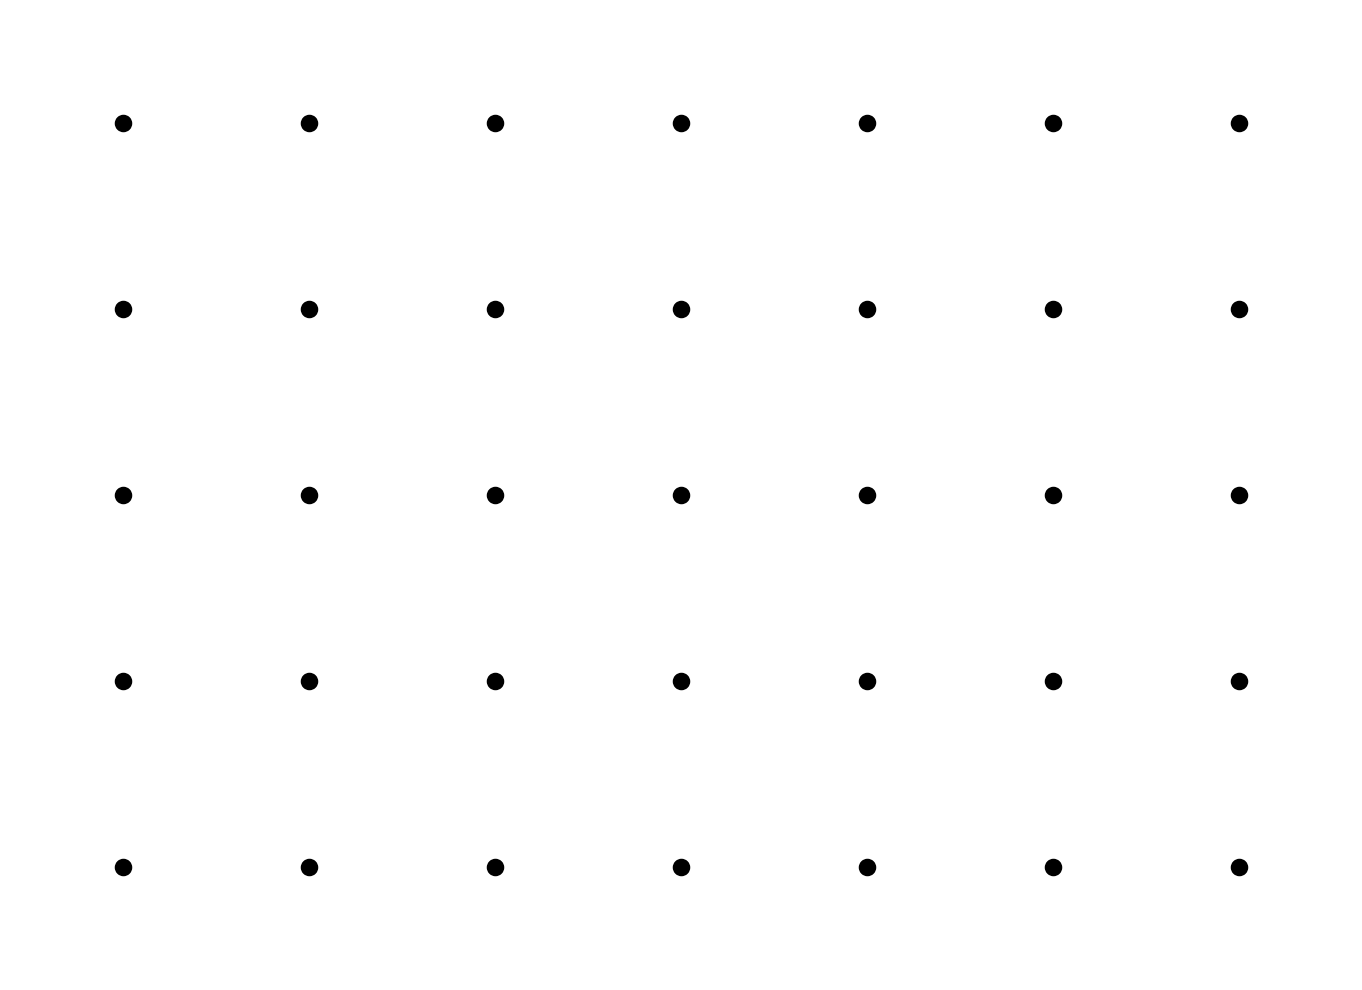
\includegraphics[width=0.62\textwidth]{fig1_6.png}
\caption{正方二维布拉维格子 $p$。}
\end{figure}

我们已说过，三维布拉维格子是无穷的点阵列，其中每个点都有相同的环境与取向。\textit{晶胞}（unit cell）可以用多种方式定义，它由三个非共面向量给出，这三个向量构成平行六面体的棱。记号 $\mathbf{a}$、$\mathbf{b}$、$\mathbf{c}$ 用于表示这三个向量。通常总是这样选取晶胞矢量，使晶胞明显体现格子的对称性；这种惯用的晶胞取法可能不是初基的，也就是说它可能含有不止一个（等价的）格点。建立在布拉维格子三个基本矢量 $\mathbf{t}_{1}$、$\mathbf{t}_{2}$、$\mathbf{t}_{3}$（式 (1.5.1)）之上的平行六面体称为\textit{初基晶胞}（primitive unit cell）。在惯用晶胞与初基晶胞不一致的每个布拉维格子中，都可以建立两者之间的关系；例如《X 射线晶体学国际表》的表 2.2.2 即做此事。图 1.7 中画出的晶胞是惯用晶胞。14 个布拉维格子各自的 $\mathbf{t}_{1}$、$\mathbf{t}_{2}$、$\mathbf{t}_{3}$ 的具体规定将在第 3 章（表 3.1）给出。惯用晶胞与初基晶胞的区别可以用二维例子说明：二维初基长方布拉维格子 $p$ 的格点排在一系列长方形的角点上，惯用晶胞就是其中一个长方形（见图 1.8(\textit{a})），它同时也是该格子的一个初基晶胞。若在每个这样的晶胞中心加一个点，就得到新的布拉维格子——心行长方布拉维格子 $c$，见图 1.8(\textit{b})。图中画出体现长方对称性的惯用晶胞（虚线）和一个初基晶胞（实线）：惯用晶胞实际含两个格点，而初基晶胞只含一个。有时还使用另一种晶胞——\textit{维格纳--赛茨原胞}（Wigner--Seitz unit cell，Wigner and Seitz 1933）。取格子上任一点 $O$ 为原点，作垂直平分 $O$ 与其最近邻（有时还包括次近邻）连线的平面族，由这些平面围成的晶胞称为维格纳--赛茨原胞；这类原胞的图示可参见 Delaunay（1932）。

布拉维格子如我们所描述的那样，是只有位置而没有大小和形状的数学点的阵列。现在我们希望在讨论中纳入构成晶体的原子或分子。实际上，我们是在每个布拉维格点上安置一组相同的原子或分子，而这组原子或分子本身必须具有与该晶体布拉维格子点群对称性相容的对称性。晶体的一种对称操作将是某种复合操作：先作某个点群操作，再作布拉维格子的一个平移 $\mathbf{t}$（见式 (1.5.1)）。于是，一种特别简单的\textit{空间群}（space group）就这样产生：让布拉维格子的每一点都联系着同一晶系的一个点群。这样可以得到 $\sum_{i=1}^{7} n_{i}p_{i}$ 个空间群，其中 $n_{i}$ 是某晶系中点群的数目，$p_{i}$ 是该晶系中布拉维格子的数目，下标 $i$ 遍历七个晶系。例如，立方晶系有 3 种布拉维格子和 5 个立方点群，因此可以用这种方法导出 15 个立方空间群。这种形式的空间群称为\textit{点式}（symmorphic）空间群，它是平移群与一个点群的半直积。半直积群的理论将在第 4 章讨论。上式并不能立即涵盖所有点式空间群，原因有二。其一，可以把三方点群与六方布拉维格子相联系：因此对三方晶系必须取 $p_{i} = 2$，尽管三方晶系只有一种布拉维格子。其二，实际上有时一个点群在布拉维格子上可能存在两种不同且可区分的取向；这导致少数额外的点式空间群不规则地出现在表 1.7 的第 6 列中。点式空间群实际上共有 73 个。

在点式空间群中，点群操作与平移群操作基本可以分开，出现的点群操作本身就是晶体的对称操作。第二类空间群可以从点式空间群出发，把某些反射面换成滑移反射面、把某些转动轴换成螺旋轴而得到；它们通常分别称为滑移面与螺旋轴。滑移反射操作是一种复合操作：先关于平面 $m$ 作反射，再平移 $\mathbf{v}$——$\mathbf{v}$ 往往（但不必然）就在平面 $m$ 内。接连两次这样的滑移反射操作的结果，必然是布拉维格子平移群中的一个平移。类似地可以有你这样的 $n$ 阶螺旋轴：螺旋旋转操作是绕轴转过 $2\pi/n$ 后再平移 $\mathbf{v}$，$\mathbf{v}$ 往往（但不必然）沿转轴方向。若这个螺旋旋转操作接连施行 $n$ 次，结果必是布拉维格子平移群中的一个纯平移。加入滑移反射面与螺旋轴后，可以再导出 157 个空间群，称为\textit{非点式空间群}（non-symmorphic space groups）或\textit{非点式空间群}（asymmorphic space groups）。可以附加条件：每个滑移反射操作的平移部分必须位于反射面自身之内，每个螺旋旋转操作的平移部分必须沿转轴方向。若施加这一条件，则当滑移面或螺旋轴存在时，对称元素就不再都作用在晶体的同一点上。此时总可以把算符变换到同一点上作用，但平移将失去"沿螺旋轴方向"或"在滑移面内"的意义，可能变成某个奇怪的方向。前一种看法在直观上更令人满意，后一种看法则对系统的数学处理必不可少；我们因此采用如下约定：所有空间群操作都在一点上作用。157 个非点式空间群与 73 个点式空间群合计 230 个空间群。它们在各晶系中的分布见表 1.7。

\begin{table}[H]
\centering
\textbf{表 1.7}\quad \textit{230 个空间群的分类}

\smallskip
\begin{tabular}{|l|c|c|c|c|c|c|c|c|}
\hline
晶系 & $s$ & $n_{i}$ & $p_{i}$ & $n_{i}p_{i}$ & 第 6 列 & 第 7 列 & 第 8 列 & 第 9 列 \\ \hline
三斜 & 1 & 2 & 1 & 2 & & 2 & & 2 \\ \hline
单斜 & 2 & 3 & 2 & 6 & & 6 & 7 & 13 \\ \hline
正交 & -- & 3 & 4 & 12 & 1 & 13 & 46 & 59 \\ \hline
四方 & 4 & 7 & 2 & 14 & 2 & 16 & 52 & 68 \\ \hline
三方 & 3 & 5 & 2 & 10 & 3 & 13 & 12 & 25 \\ \hline
六方 & 6 & 7 & 1 & 7 & 1 & 8 & 19 & 27 \\ \hline
立方 & & 5 & 3 & 15 & & 15 & 21 & 36 \\ \hline
\textbf{总计} & -- & 32 & 15 & 66 & 7 & 73 & 157 & 230 \\ \hline
\end{tabular}

\smallskip
\parbox{0.92\textwidth}{\textit{表 1.7 的注.}
(i) $s$ 是主轴存在时的阶数。主轴上的操作可以是真转动，也可以是非真转动。
(ii) $n_{i}$ 是给定晶系的点群数目。注意 $\bar{6}$（$C_{3h}$）与 $\bar{6}2m$（$D_{3h}$）必须归入六方晶系。$p_{i}$ 是给定晶系的布拉维格子数目，三方晶系例外，取 $p_{i} = 2$：因为如正文所释，每个三方点群都可以与六方布拉维格子相联系，故该格子总计被计了两次。
(iii) 第 6 列是由于某些点群在布拉维格子上有可区分的不同定向而出现的点式空间群数目。第 7、8 列分别是给定晶系的点式与非点式空间群总数。第 9 列是给定晶系两类空间群的总数。}
\end{table}

\needspace{5\baselineskip}
\textit{空间群算符的 Seitz 记号}

表示一般空间群操作的一个方便记号是 $\{R \,|\, \mathbf{v}\}$，其中 $R$ 是点群算符，$\mathbf{v}$ 是与之相联系的平移向量；该算符的解释是：它作用在空间的点上，而这些点总是相对一组固定的轴给出，即它是\textit{主动}算符（见 1.4 节）。符号 $\{R \,|\, \mathbf{v}\}$ 由 Seitz（1936\textsuperscript{b}）引入，称为 \textit{Seitz 空间群符号}。由于这些算符是主动的，$\{R_{1} \,|\, \mathbf{v}_{1}\}$ 作用在向量 $\mathbf{r}$ 上产生 $\mathbf{r}'$：

\begin{equation*}
\{R_{1} \,|\, \mathbf{v}_{1}\}\mathbf{r} = \mathbf{r}' = R_{1}\mathbf{r} + \mathbf{v}_{1},
\tag{1.5.2}
\end{equation*}

其中 $R_{1}\mathbf{r}$ 是主动点群算符 $R_{1}$ 作用在 $\mathbf{r}$ 上得到的向量。这些算符的乘法有一条简单而重要的规则：

\begin{equation*}
\{R_{2} \,|\, \mathbf{v}_{2}\}\{R_{1} \,|\, \mathbf{v}_{1}\} = \{R_{2}R_{1} \,|\, \mathbf{v}_{2} + R_{2}\mathbf{v}_{1}\}
\tag{1.5.3}
\end{equation*}

把 $\{R_{2} \,|\, \mathbf{v}_{2}\}$ 作用在式 (1.5.2) 两边即可容易验证。由式 (1.5.3) 立即得到 $\{R_{1} \,|\, \mathbf{v}_{1}\}$ 的逆为 $\{R_{1}^{-1} | -R_{1}^{-1}\mathbf{v}_{1}\}$。全部 230 个空间群的 Seitz 算符已被多位作者整理（Faddeev 1964，Henry and Lonsdale 1965，Koptsik 1966，Kovalev 1965，Lyubarskii 1960，Miller and Love 1967），并列于第 3 章。

\textit{空间群标记的记号}

空间群首先按其所属晶系分类；进一步的分类取决于想传达多少信息。可以标记空间群所\textit{同形}（isogonal）的点群——即从空间群的操作中取出所有点群算符所组成的点群。\footnote{有些作者用 isomorphous（同晶）一词表示我们这里的 isogonal（同形）。} 这正是使用 Schönflies 记号（Hilton 1903）时的立场：空间群被赋予其同形点群的 Schönflies 标记，同形于同一有理点群的不同空间群则以一个任意的区分上标相区别——该上标仅仅反映 Schönflies（1891）推导空间群的先后次序。例如，与立方点群 $O_{h}$（$m3m$）同形的空间群有 10 个，分布在三种立方布拉维格子上：四个初基、四个面心、两个体心，记作 $O_{h}^{1}, O_{h}^{2}, \ldots, O_{h}^{10}$。这种记号有两个缺点。其一，一眼看不出空间群建立在哪种布拉维格子上：例如 $O_{h}^{8}$ 是面心的，$O_{h}^{6}$ 是体心的。其二，看不出空间群是点式还是非点式的。更随意的方案是给每个空间群一个 1 到 230 之间的编号，由 Astbury and Yardley（1924）提出，并被收入《X 射线晶体学国际表》（Henry and Lonsdale 1965）。

Schönflies 记号的这两个缺点在使用国际记号时都被克服了：国际记号不仅确定上述两点，还给出空间群中对称元素的性质与取向的某些信息（Hermann 1928\textsuperscript{a}，Mauguin 1931，Schiebold 1929）。做法是在国际点群符号（例如 $m3m$）前加一个描述布拉维格子的字母——$P$、$F$、$I$ 分别表示初基、面心、体心——于是得到 $Pm3m$、$Fm3m$、$Im3m$。这三个符号表示与点群 $m3m$（$O_{h}$）同形的三个点式空间群。当一个点群在布拉维格子上可以有多种取向时（例如四方晶系中的 $\bar{4}2m$（$D_{2d}$）），可以赋予国际空间群符号中字符次序以特定的含义；于是 $P\bar{4}2m$（$D_{2d}$）与 $P\bar{4}m2$（$D_{2d}$）是不同的空间群。对非点式空间群，符号按下述方式修改：凡被滑移面代替的反射面，符号中相应部分换成另一个表示滑移面的字母；例如 $Fd3m$（$O_{h}^{7}$）——金刚石结构的空间群——是面心的、非点式的，具有对角方向的滑移面。其他字母还有晶轴方向 $a$、$b$、$c$。对螺旋轴，空间群符号中表示该轴阶数的部分（例如 $P432$ 中的 4）换成同一符号加上一个表示螺旋轴平移量大小的后缀；于是 $P4_{1}32$（$O^{7}$）——与点群 432（$O$）同形的立方空间群之一——是初基的，其四次转动轴换成四次螺旋轴，即每次四次转动伴随晶格矢量在该方向四分之一长度的平移。国际记号并不完美，但它广为人知、经过仔细鉴定（Henry and Lonsdale 1965）并被广泛接受。这一记号的原始形式见旧版《X 射线晶体学国际表》（Bragg, von Laue, and Hermann 1935\textsuperscript{a}, \textsuperscript{b}），后来的修改见新版（Henry and Lonsdale 1965）；如何在鉴定空间群时使用这些表将在第 3 章（3.5 节）进一步讨论。本书提到点群或空间群时，一律用国际符号加括号内的 Schönflies 符号。

\textit{函数空间算符}

若 $R$ 是 Seitz 空间群算符的转动部分，即 $R$ 是一个点群操作，则每个算符 $R$ 通过如下类型的方程作用在空间的点 $\mathbf{r}$ 上（类似式 (1.4.8)）：

\begin{equation*}
R\mathbf{r} = \mathbf{r}'.
\tag{1.5.4}
\end{equation*}

若定义了标量函数 $f(\mathbf{r})$，则点 $\mathbf{r}$ 的移动会引起函数的相应变化。新函数满足：新函数在变换后点的取值等于原函数在原点的取值，即

\begin{equation*}
g(\mathbf{r}') = f(\mathbf{r}).
\tag{1.5.5}
\end{equation*}

习惯上记 $g = \bar{R}f$，即对每个算符 $R$ 定义了一个对应的\textit{函数空间算符}（function space operator）$\bar{R}$。由式 (1.5.4) 与 (1.5.5) 得

\begin{equation*}
\bar{R}f(\mathbf{r}) = f(R^{-1}\mathbf{r}).
\tag{1.5.6}
\end{equation*}

遗憾的是，多数作者并不为 $\bar{R}$ 使用单独的符号；事实上，只要仔细区分算符作用在函数上还是作用在向量上，就无须单独的符号。处理函数空间算符时必须按式 (1.5.6) 进行。下面的例子足以作为警示。

\textit{例} 1.5.1. 取 $\mathbf{r} = x\mathbf{i} + y\mathbf{j} + z\mathbf{k}$，定义 $f(\mathbf{r}) = x$，$g(\mathbf{r}) = y$，$h(\mathbf{r}) = z$，即向量 $\mathbf{r}$ 在三个坐标方向的投影。则

\begin{equation*}
\bar{C}_{4z}^{+}f(\mathbf{r}) = f(C_{4z}^{+}\mathbf{r}),
\tag{1.5.7}
\end{equation*}

它等于 $f(y\mathbf{i} - x\mathbf{j} + z\mathbf{k})$（见表 1.4 的注 (iii)）。自变量在 $\mathbf{i}$ 方向的投影是 $y$，因此

\begin{equation*}
\bar{C}_{4z}^{+}f(\mathbf{r}) = y = g(\mathbf{r}).
\tag{1.5.8}
\end{equation*}

于是在符号层面上既有 $C_{4z}^{+}\mathbf{i} = \mathbf{j}$，又有 $\bar{C}_{4z}^{+}f = g$。事实上，以基 $\langle \mathbf{i}, \mathbf{j}, \mathbf{k}|$ 表示算符 $C_{4z}^{+}$ 的矩阵，与以基 $\langle f, g, h|$ 表示函数空间算符 $\bar{C}_{4z}^{+}$ 的矩阵是相同的。在提醒过要小心之后，这倒是一个人们几乎不敢期望其为真的结果。

\textit{例} 1.5.2. 设 $\phi$ 是方位角（$x$ 轴与位置矢量在 $xy$ 平面上投影之间的夹角）。则

\begin{equation*}
C_{4z}^{+}\phi = \phi + \tfrac{1}{2}\pi
\tag{1.5.9}
\end{equation*}

但把 $\bar{C}_{4z}^{+}$ 作为函数空间算符时必须写

\begin{equation*}
\bar{C}_{4z}^{+}\cos\phi = \cos(C_{4z}^{-}\phi) = \cos(\phi - \tfrac{1}{2}\pi) = \sin\phi.
\tag{1.5.10}
\end{equation*}

式 (1.5.10) 也可以由式 (1.5.8) 推出：因为 $f(\mathbf{r}) = r\sin\theta\cos\phi$，$g(\mathbf{r}) = r\sin\theta\sin\phi$，而 $C_{4z}^{+}$ 不改变 $r$ 与 $\theta$。还应注意，由于 $\cos(\phi + \tfrac{1}{2}\pi) = -\sin\phi$，有 $C_{4z}^{+}\cos\phi \neq \cos(C_{4z}^{+}\phi)$。

\textit{主动与被动空间群算符}

如前所述，主动算符移动空间的点或位置矢量，所有矢量都相对一组固定的轴给出。本书使用的 Seitz 空间群算符是主动的，由式 (1.5.2) 定义：

\begin{equation*}
\{R_{a} \,|\, \mathbf{v}\}\mathbf{r} = R_{a}\mathbf{r} + \mathbf{v},
\tag{1.5.11}
\end{equation*}

其中用下标 $a$ 强调这是主动算符。也就是说，先作主动转动 $R_{a}$ 使 $\mathbf{r} \rightarrow R_{a}\mathbf{r}$，再对新位置矢量作平移 $+\mathbf{v}$，结果为 $(R_{a}\mathbf{r} + \mathbf{v})$。主动 Seitz 空间群算符的乘法规则已在式 (1.5.3) 中得到：

\begin{equation*}
\{S_{a} \,|\, \mathbf{w}\}\{R_{a} \,|\, \mathbf{v}\} = \{S_{a}R_{a} \,|\, \mathbf{w} + S_{a}\mathbf{v}\}.
\tag{1.5.12}
\end{equation*}

$\{R_{a} \,|\, \mathbf{v}\}$ 的逆为

\begin{equation*}
\{R_{a} \,|\, \mathbf{v}\}^{-1} = \{R_{a}^{-1} \,|\, -R_{a}^{-1}\mathbf{v}\}.
\tag{1.5.13}
\end{equation*}

被动算符移动空间的坐标轴，而空间的所有点从而所有矢量位置保持不动，于是每次操作之后矢量位置都相对一组新的坐标轴给出。也可以定义被动空间群算符（Johnston 1960）。为与主动 Seitz 算符区分，使用方括号 $[R_{p} \,|\, \mathbf{v}]$，对应于式 (1.5.11) 的定义规则是

\begin{equation*}
[R_{p} \,|\, \mathbf{v}]\mathbf{r} = R_{p}\mathbf{r} - R_{p}\mathbf{v}.
\tag{1.5.14}
\end{equation*}

也就是说，先把轴平移 $+\mathbf{v}$，使 $\mathbf{r} \rightarrow (\mathbf{r} - \mathbf{v})$，再转动新轴，最终结果为 $(R_{p}\mathbf{r} - R_{p}\mathbf{v})$，其中 $R_{p}$ 现在是被动转动。这些被动算符的乘法规则是

\begin{equation*}
[S_{p} \,|\, \mathbf{w}][R_{p} \,|\, \mathbf{v}] = [S_{p}R_{p} \,|\, \mathbf{v} + R_{p}^{-1}\mathbf{w}]
\tag{1.5.15}
\end{equation*}

而 $[R_{p} \,|\, \mathbf{v}]$ 的逆为

\begin{equation*}
[R_{p} \,|\, \mathbf{v}]^{-1} = [R_{p}^{-1} \,|\, -R_{p}\mathbf{v}].
\tag{1.5.16}
\end{equation*}

若 $X$ 是一个算符——无论主动还是被动——则与 $X$ 一起还有另一个算符 $\bar{X}$：$\bar{X}$ 是式 (1.5.4)--(1.5.6) 定义的函数空间算符。若 $f(\mathbf{r})$ 是位置的标量函数，则

\begin{equation*}
\bar{X}f(\mathbf{r}) = f(X^{-1}\mathbf{r}).
\tag{1.5.17}
\end{equation*}

必须认识到 $(\bar{X}f)$ 是一个函数的记号，正如 $f$ 也是函数的记号。式 (1.5.17) 并非随意规定，它陈述了如下事实：变换后的函数 $(\bar{X}f)$ 在变换后的点 $X\mathbf{r}$ 处的取值，等于 $f$ 在点 $\mathbf{r}$ 处的取值。Wigner（1959）强调过的另一点也必须再次强调：若 $Z = YX$，则要求 $\bar{Z}f = \bar{Y}\bar{X}f$，因为我们要在算符群与相应的函数空间算符群之间保持同构。证明只需反复应用式 (1.5.17)。记 $\bar{X}f = g$，则

\begin{align*}
\bar{Y}\bar{X}f(\mathbf{r}) &= \bar{Y}g(\mathbf{r}), \\
&= g(Y^{-1}\mathbf{r}) &&\text{（由式 (1.5.17)）}, \\
&= \bar{X}f(Y^{-1}\mathbf{r}) &&\text{（因 } \bar{X}f = g\text{）}, \\
&= f(X^{-1}Y^{-1}\mathbf{r}) &&\text{（由式 (1.5.17)）}, \\
&= f(Z^{-1}\mathbf{r}) &&\text{（因 } Z = YX\text{）}, \\
&= \bar{Z}f(\mathbf{r}) &&\text{（再次由式 (1.5.17)）}.
\end{align*}

于是如所要求的有 $\bar{Y}\bar{X}f = \bar{Z}f$。直接对式 (1.5.17) 作用 $\bar{Y}$ 是错误的，因为式 (1.5.17) 是关于两个函数在不同自变量取值下的数值关系，而算符不能作用于数（Altmann and Bradley 1965，Slater 1965\textsuperscript{a}）。

作为第一个例子，考虑被动空间群算符对函数 $\psi(\mathbf{r})$ 的作用。由式 (1.5.17) 得

\begin{align*}
\overline{[S_{p} \,|\, \mathbf{w}]}\,\psi(\mathbf{r}) &= \psi([S_{p} \,|\, \mathbf{w}]^{-1}\mathbf{r}) \\
&= \psi([S_{p}^{-1} \,|\, -S_{p}\mathbf{w}]\mathbf{r}) &&\text{（由式 (1.5.16)）} \tag{1.5.18}\\
&= \psi(S_{p}^{-1}\mathbf{r} + \mathbf{w}) &&\text{（由式 (1.5.14)）}. \tag{1.5.19}
\end{align*}

由函数空间算符的乘法规则与式 (1.5.19)，

\begin{align*}
\overline{[S_{p} \,|\, \mathbf{w}]}\,\overline{[R_{p} \,|\, \mathbf{v}]}\,\psi(\mathbf{r}) &= \overline{[R_{p} \,|\, \mathbf{v}]}\,\psi(S_{p}^{-1}\mathbf{r} + \mathbf{w}) \\
&= \psi(R_{p}^{-1}S_{p}^{-1}\mathbf{r} + R_{p}^{-1}\mathbf{w} + \mathbf{v}). \tag{1.5.20}
\end{align*}

从式 (1.5.19) 出发按如下方式“推导”式 (1.5.20) 是不正确的：

\begin{align*}
\overline{[S_{p} \,|\, \mathbf{w}]}\,\overline{[R_{p} \,|\, \mathbf{v}]}\,\psi(\mathbf{r}) &= \overline{[S_{p} \,|\, \mathbf{w}]}\,\psi(R_{p}^{-1}\mathbf{r} + \mathbf{v}) \tag{1.5.21}\\
&= \psi(R_{p}^{-1}(S_{p}^{-1}\mathbf{r} + \mathbf{w}) + \mathbf{v}) \tag{1.5.22}\\
&= \psi(R_{p}^{-1}S_{p}^{-1}\mathbf{r} + R_{p}^{-1}\mathbf{w} + \mathbf{v}). \tag{1.5.20}
\end{align*}

式 (1.5.21) 之所以错误，是因为如上所述 $[S_{p} \,|\, \mathbf{w}]$ 不能直接作用于数值关系 $[R_{p} \,|\, \mathbf{v}]\psi(\mathbf{r}) = \psi(R_{p}^{-1}\mathbf{r} + \mathbf{v})$；退一步说即使可以，式 (1.5.22) 也不对，并且直接违背数学惯例：函数空间算符作用于函数的整个自变量，而不是只作用于其中的 $\mathbf{r}$ 部分。

对主动空间群算符，与式 (1.5.19)、(1.5.20) 相应的方程是

\begin{equation*}
\overline{\{S_{a} \,|\, \mathbf{w}\}}\,\psi(\mathbf{r}) = \psi(S_{a}^{-1}(\mathbf{r} - \mathbf{w}))
\tag{1.5.23}
\end{equation*}

以及

\begin{equation*}
\overline{\{S_{a} \,|\, \mathbf{w}\}}\,\overline{\{R_{a} \,|\, \mathbf{v}\}}\,\psi(\mathbf{r}) = \psi(R_{a}^{-1}S_{a}^{-1}\mathbf{r} - R_{a}^{-1}S_{a}^{-1}\mathbf{w} - R_{a}^{-1}\mathbf{v}).
\tag{1.5.24}
\end{equation*}

式 (1.5.19) 与 (1.5.23) 加上 $S_{p} = S_{a}^{-1}$ 这一事实，蕴涵 $[S_{p} \,|\, \mathbf{w}] = \{S_{a} \,|\, \mathbf{w}\}^{-1}$——这正是我们应当期望的主动算符与被动算符之间的关系。

\textit{例} 1.5.3. 令 $\{E \,|\, \mathbf{t}\}$ 表示平移 $\mathbf{t}$。则

\begin{equation*}
\{E \,|\, \mathbf{t}\}\mathbf{r} = \mathbf{r} + \mathbf{t}.
\tag{1.5.25}
\end{equation*}

而若 $\{E \,|\, \mathbf{t}\}$ 作用在函数 $\psi(\mathbf{r})$ 而非向量 $\mathbf{r}$ 上，则有

\begin{equation*}
\overline{\{E \,|\, \mathbf{t}\}}\,\psi(\mathbf{r}) = \psi(\{E \,|\, \mathbf{t}\}^{-1}\mathbf{r}) = \psi(\mathbf{r} - \mathbf{t}).
\tag{1.5.26}
\end{equation*}

如前所述，本书一律使用主动点群算符与主动空间群算符；只是偶尔举例说明：若选用被动算符，我们的理论讨论需要作哪些修改。


% 第二章
\chapter{点群的对称适配函数}
% 第二章（章标题见 ch2.tex）

本章的目的是推导属于晶体学点群矩阵表示各行的球谐函数线性组合，并给出这些函数的表。Melvin（1956）把这类函数命名为\textit{对称适配函数}（symmetry-adapted functions），因为它们在群元素变换下具有表示所要求的正确性质。在确定对称适配函数方面做过工作的有：Altmann（1956, 1957），Bell（1954），Bethe（1929），Betts（1959），Callen and Callen（1963），Cohan（1958），Cornwell（1969），Flodmark（1963），Flower, March, and Murray（1960），McIntosh（1960\textsuperscript{a}, 1963），Melvin（1956），Meyer（1954），Nesbet（1961），Schiff（1955, 1956），以及 von der Lage and Bethe（1947）。本章的处理相当紧贴 Altmann（1957）、Altmann and Bradley（1963\textsuperscript{a}, \textsuperscript{b}, 1965）与 Altmann and Cracknell（1965）给出的路线。给定群的一个矩阵表示，问题就是求出对该表示对称适配的所有可能的基。于是，任何可以按球谐函数展开、且要具有该表示某一行的变换性质的函数，都将只包含那些对称适配到同一变换性质的球谐函数线性组合。我们对这样的、对称适配到点群表示某一行的球谐函数线性组合使用术语\textit{面谐函数}（surface harmonic）。

\section{转动群的矩阵元}

在确定对称适配函数的过程中，需要知道球谐函数在三维转动群的各类转动下如何变换。本节给出确定这些变换性质所需的公式与定义。

我们采用如下归一化球谐函数的定义：

\begin{equation*}
Y_{l}^{m}(\theta, \phi) = \sqrt{\left\{\frac{(2l+1)(l-|m|)!}{4\pi(l+|m|)!}\right\}}\, P_{l}^{m}(\cos\theta)\exp(\mathrm{i}m\phi)
\tag{2.1.1}
\end{equation*}

其中 $P_{l}^{m}(\cos\theta)$ 是连带勒让德函数：

\begin{equation*}
P_{l}^{m}(\cos\theta) = \frac{1}{2^{l}l!}\sin^{|m|}\theta\ \frac{d^{l+|m|}}{(d\cos\theta)^{l+|m|}}\left\{(\cos^{2}\theta - 1)^{l}\right\}.
\tag{2.1.2}
\end{equation*}

这里不宜赘述球谐函数的性质——讨论它们的书非常多（仅举数例：Condon and Shortley (1935)，Edmonds (1957)，Gel'fand, Minlos, and Shapiro (1963)，Wigner (1959)）。

我们用欧拉角 $\alpha$、$\beta$、$\gamma$ 规定一个纯转动 $R$：先绕 $z$ 轴作角度 $\alpha$（$0 \leqslant \alpha < 2\pi$）的主动转动，其次绕 $y$ 轴作角度 $\beta$（$0 \leqslant \beta \leqslant \pi$）的主动转动，最后绕 $z$ 轴作角度 $\gamma$（$0 \leqslant \gamma < 2\pi$）的主动转动。于是第一次转动（转角 $\alpha$）把点 $(r, \theta, \phi)$ 移到 $(r, \theta, \phi + \alpha)$；第二次转动（转角 $\beta$）把点 $(r, \theta, 0)$ 移到 $(r, \theta + \beta, 0)$；第三次转动（转角 $\gamma$）把点 $(r, \theta, \phi)$ 移到 $(r, \theta, \phi + \gamma)$（见图 2.1）。$R(\alpha, \beta, \gamma)$ 表示这三个相继转动的乘积。注意，与全书一致，我们采用主动约定：算符 $R(\alpha, \beta, \gamma)$ 移动空间的点而保持坐标系 $Oxyz$ 不动；并且所有正向转动都取通常的逆时针方向。

\begin{figure}[H]
\centering
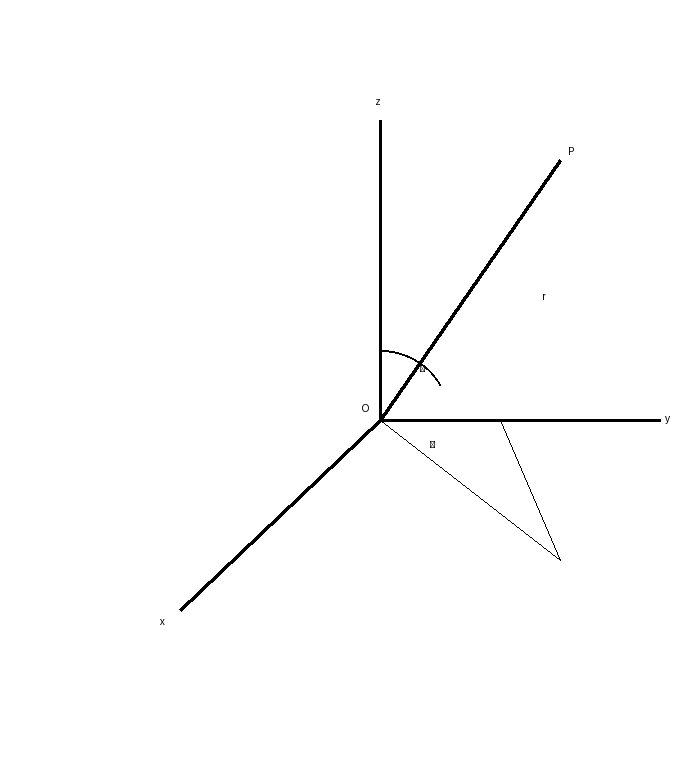
\includegraphics[width=0.52\textwidth]{fig2_1.png}
\caption{球极坐标 $(r, \theta, \phi)$。}
\end{figure}

采用这一欧拉角定义，即可导出球谐函数的变换规律，结果是（Altmann 1957，Wigner 1959）

\begin{equation*}
R(\alpha, \beta, \gamma)Y_{l}^{m}(\theta, \phi) = \sum_{n=-l}^{l} Y_{l}^{n}(\theta, \phi)\mathscr{D}^{l}\{R(\alpha, \beta, \gamma)\}_{nm},
\tag{2.1.3}
\end{equation*}

其中

\begin{equation*}
\mathscr{D}^{l}\{R(\alpha, \beta, \gamma)\}_{nm} = C_{nm}\exp(-\mathrm{i}n\gamma)\, d^{l}(\beta)_{nm}\exp(-\mathrm{i}m\alpha).
\tag{2.1.4}
\end{equation*}

在式 (2.1.4) 中

\begin{equation*}
C_{nm} = (\mathrm{i}^{|n|+n})(\mathrm{i}^{-|m|-m}),
\tag{2.1.5}
\end{equation*}

而

\begin{equation*}
\begin{aligned}
d^{l}(\beta)_{nm} = \sum_{k} \frac{(-1)^{k-m+n}\sqrt{\{(l+n)!(l+m)!(l-n)!(l-m)!\}}}{(l-n-k)!(l+m-k)!k!(k-m+n)!} \\
\times \cos^{2l+m-n-2k}\left(\tfrac{1}{2}\beta\right)\sin^{2k+n-m}\left(\tfrac{1}{2}\beta\right),
\end{aligned}
\tag{2.1.6}
\end{equation*}

其中对 $k$ 的求和从数 0 与 $(m-n)$ 中较大者到数 $(l-n)$ 与 $(l+m)$ 中较小者。对三维转动群的每个转动 $R(\alpha, \beta, \gamma)$，对每个整数 $l$ 都有唯一一个矩阵 $\mathscr{D}^{l}\{R(\alpha, \beta, \gamma)\}$。对给定的 $l$，矩阵族 $\mathscr{D}^{l}\{R(\alpha, \beta, \gamma)\}$ 构成定义 1.3.4 意义下转动群 $R(\alpha, \beta, \gamma)$ 的一个 $(2l+1)$ 维表示。式 (2.1.3) 表明函数 $Y_{l}^{m}(\theta, \phi)$（$-l \leqslant m \leqslant l$）构成该表示的一组基。$\mathscr{D}^{j}\{R(\alpha, \beta, \gamma)\}$（$j$ 为半奇数）的表示将在第 6 章讨论。

约化矩阵元 $d^{l}(\beta)_{nm}$ 满足以下对称关系：

\begin{equation*}
d^{l}(\beta)_{nm} = d^{l}(\beta)_{-m,-n} = (-1)^{m+n}d^{l}(\beta)_{mn}.
\tag{2.1.7}
\end{equation*}

由于式 (2.1.7)，只需在 $-l \leqslant m \leqslant l$、$|m| \leqslant n \leqslant l$ 范围内计算 $d^{l}(\beta)_{nm}$。Altmann and Bradley（1963\textsuperscript{a}）证明，在此范围内 $d^{l}(\beta)_{nm}$ 用递推关系计算最方便：

\begin{equation*}
\begin{aligned}
\sqrt{\{(l+n)(l-n+1)\}}\, d^{l}(\beta)_{n-1,m} \\
= (m-n)\cot\left(\tfrac{1}{2}\beta\right)d^{l}(\beta)_{nm} - \sqrt{\{(l+m)(l-m+1)\}}\, d^{l}(\beta)_{n,m-1}
\end{aligned}
\tag{2.1.8}
\end{equation*}

起始值为

\begin{equation*}
d^{l}(\beta)_{lm} = (-1)^{l-m}\sqrt{\left\{\frac{(2l)!}{(l+m)!(l-m)!}\right\}}\cos^{l+m}\left(\tfrac{1}{2}\beta\right)\sin^{l-m}\left(\tfrac{1}{2}\beta\right).
\tag{2.1.9}
\end{equation*}

式 (2.1.8) 仅对 $l$、$m$、$n$ 的整数值成立。

$\beta = 0$、$\beta = \pi$ 与 $\beta = \tfrac{1}{2}\pi$ 三种情形值得特别注意，原因有二：其一，如 Wigner（1959）所示，任意 $\beta$ 的矩阵元可以由 $\beta = \tfrac{1}{2}\pi$ 的矩阵元表出；其二，总可以（Altmann 1957）选取坐标轴，使晶体学点群中任何转动的 $\beta$ 角取 $0$、$\tfrac{1}{2}\pi$、$\pi$ 三值之一。若 $\beta = 0$，则这是绕 $z$ 轴转 $(\alpha + \gamma)$ 的转动，于是

\begin{equation*}
\mathscr{D}^{l}\{R(\alpha, 0, \gamma)\}_{nm} = \exp(-\mathrm{i}m\alpha)\exp(-\mathrm{i}m\gamma)\delta_{nm}.
\tag{2.1.10}
\end{equation*}

若 $\beta = \pi$，则如 Altmann（1957）所示，仅当 $n = -m$ 时有非零元，且

\begin{equation*}
\mathscr{D}^{l}\{R(\alpha, \pi, \gamma)\}_{nm} = (-1)^{l}\exp(-\mathrm{i}m\alpha)\exp(\mathrm{i}m\gamma)\delta_{n,-m}.
\tag{2.1.11}
\end{equation*}

若 $\beta = \tfrac{1}{2}\pi$，则 $d^{l}(\tfrac{1}{2}\pi)_{nm}$ 没有简单的解析公式；不过 Bradley（1961）已对所有 $l \leqslant 20$ 的值编制了这些函数的表。

为完整研究球谐函数在点群操作下的变换性质，还需补充在反演 $I$ 下的变换关系：

\begin{equation*}
IY_{l}^{m}(\theta, \phi) = (-1)^{l}Y_{l}^{m}(\theta, \phi).
\tag{2.1.12}
\end{equation*}

第 1 章引入的晶体学点群操作的欧拉角表见表 2.1。

\begin{table}[H]
\centering
\textbf{表 2.1}\quad \textit{点群 432（$O$）与 622（$D_{6}$）的欧拉角}

\smallskip
\resizebox{\textwidth}{!}{%
\begin{tabular}{|c|c|c|c||c|c|c|c||c|c|c|c|}
\hline
\multicolumn{8}{|c||}{(a) 432（$O$）} & \multicolumn{4}{c|}{(b) 622（$D_{6}$）} \\ \hline
元素 & $\alpha$ & $\beta$ & $\gamma$ & 元素 & $\alpha$ & $\beta$ & $\gamma$ & 元素 & $\alpha$ & $\beta$ & $\gamma$ \\ \hline
$E$ & $0$ & $0$ & $0$ & $C_{4x}^{+}$ & $\tfrac{1}{2}\pi$ & $\tfrac{1}{2}\pi$ & $\tfrac{3}{2}\pi$ & $E$ & $0$ & $0$ & $0$ \\ \hline
$C_{2x}$ & $\pi$ & $\pi$ & $0$ & $C_{4y}^{+}$ & $0$ & $\tfrac{1}{2}\pi$ & $0$ & $C_{6}^{+}$ & $\tfrac{1}{3}\pi$ & $0$ & $0$ \\ \hline
$C_{2y}$ & $0$ & $\pi$ & $0$ & $C_{4z}^{+}$ & $\tfrac{1}{2}\pi$ & $0$ & $0$ & $C_{3}^{+}$ & $\tfrac{2}{3}\pi$ & $0$ & $0$ \\ \hline
$C_{2z}$ & $\pi$ & $0$ & $0$ & $C_{4x}^{-}$ & $\tfrac{3}{2}\pi$ & $\tfrac{1}{2}\pi$ & $\tfrac{1}{2}\pi$ & $C_{2}$ & $\pi$ & $0$ & $0$ \\ \hline
$C_{31}^{-}$ & $\tfrac{1}{2}\pi$ & $\tfrac{1}{2}\pi$ & $0$ & $C_{4y}^{-}$ & $\pi$ & $\tfrac{1}{2}\pi$ & $\pi$ & $C_{3}^{-}$ & $\tfrac{4}{3}\pi$ & $0$ & $0$ \\ \hline
$C_{32}^{+}$ & $\tfrac{3}{2}\pi$ & $\tfrac{1}{2}\pi$ & $\pi$ & $C_{4z}^{-}$ & $\tfrac{3}{2}\pi$ & $0$ & $0$ & $C_{6}^{-}$ & $\tfrac{5}{3}\pi$ & $0$ & $0$ \\ \hline
$C_{33}^{+}$ & $\tfrac{1}{2}\pi$ & $\tfrac{1}{2}\pi$ & $\pi$ & $C_{2a}$ & $\tfrac{1}{2}\pi$ & $\pi$ & $0$ & $C'_{21}$ & $\pi$ & $\pi$ & $0$ \\ \hline
$C_{34}^{+}$ & $\tfrac{3}{2}\pi$ & $\tfrac{1}{2}\pi$ & $0$ & $C_{2b}$ & $\tfrac{3}{2}\pi$ & $\pi$ & $0$ & $C'_{22}$ & $\tfrac{5}{3}\pi$ & $\pi$ & $0$ \\ \hline
$C_{31}^{+}$ & $\pi$ & $\tfrac{1}{2}\pi$ & $\tfrac{1}{2}\pi$ & $C_{2c}$ & $\pi$ & $\tfrac{1}{2}\pi$ & $0$ & $C'_{23}$ & $\tfrac{1}{3}\pi$ & $\pi$ & $0$ \\ \hline
$C_{32}^{-}$ & $0$ & $\tfrac{1}{2}\pi$ & $\tfrac{3}{2}\pi$ & $C_{2d}$ & $\tfrac{1}{2}\pi$ & $\tfrac{1}{2}\pi$ & $\tfrac{1}{2}\pi$ & $C''_{21}$ & $0$ & $\pi$ & $0$ \\ \hline
$C_{33}^{-}$ & $0$ & $\tfrac{1}{2}\pi$ & $\tfrac{1}{2}\pi$ & $C_{2e}$ & $0$ & $\tfrac{1}{2}\pi$ & $\pi$ & $C''_{22}$ & $\tfrac{2}{3}\pi$ & $\pi$ & $0$ \\ \hline
$C_{34}^{-}$ & $\pi$ & $\tfrac{1}{2}\pi$ & $\tfrac{3}{2}\pi$ & $C_{2f}$ & $\tfrac{3}{2}\pi$ & $\tfrac{1}{2}\pi$ & $\tfrac{3}{2}\pi$ & $C''_{23}$ & $\tfrac{4}{3}\pi$ & $\pi$ & $0$ \\ \hline
\end{tabular}}

\smallskip
\parbox{0.92\textwidth}{\textit{表 2.1 的注.}
(i) 对称操作已在第 1 章定义，均为主动操作。
(ii) 欧拉角定义为：先将空间的点绕 $z$ 轴转 $\alpha$（正向规定为 $x$ 轴上的点转向 $y$ 轴），随后绕 $y$ 轴转 $\beta$，再绕 $z$ 轴转 $\gamma$。$\alpha$、$\beta$、$\gamma$ 的限制为 $0 \leqslant \alpha < 2\pi$、$0 \leqslant \beta \leqslant \pi$、$0 \leqslant \gamma < 2\pi$。}
\end{table}

% 2.2 生成对称适配函数；2.3 应用于点群
\section{对称适配函数的生成}

本节给出求属于任何有限群不可约表示的对称适配函数的一般规则。

设 $\mathbf{G}$ 是阶为 $|\mathbf{G}|$ 的群，元素为 $R, S, \ldots$ 等；再设其表示为 $\Gamma^{i}\{R \rightarrow \mathbf{D}^{i}(R)\}$，且为已知。这里 $\mathbf{D}^{i}(R)$ 是 $R$ 的矩阵表示元，维数设为 $d_{i}$。问题是求一组基 $\langle \phi_{1}^{i}, \phi_{2}^{i}, \ldots, \phi_{d_{i}}^{i}|$，使得

\begin{equation*}
R\phi_{s}^{i} = \sum_{t=1}^{d_{i}} \phi_{t}^{i}\mathbf{D}^{i}(R)_{ts}
\tag{2.2.1}
\end{equation*}

对一切 $R \in \mathbf{G}$ 成立。$\phi_{s}^{i}$ 便称为属于表示 $\Gamma^{i}$ 第 $s$ 行的对称适配函数。实际上要找的不只是一组基，而是一整套基，使得全部函数 $\phi_{s}^{i}$（对所有 $s$ 与所有 $i$）在群算符实现于其中的线性空间 $V$ 中构成完备集。确定这类函数的理论是群论的一个直接应用。

可以如下定义群环的元素 $W_{ts}^{i}$：

\begin{equation*}
W_{ts}^{i} = \frac{d_{i}}{|\mathbf{G}|} \sum_{R \in \mathbf{G}} \mathbf{D}^{i}(R)_{ts}^{*} R
\tag{2.2.2}
\end{equation*}

其中求和遍历所有 $R \in \mathbf{G}$。

\textbf{定理 2.2.1.} \textit{若 $\phi$ 是 $V$ 中满足 $W_{ss}^{i}\phi \neq 0$ 的任意函数（$s$ 固定，取 1 到 $d_{i}$ 之间的值），则函数 $W_{ts}^{i}\phi = \phi_{t}^{i}$（$t = 1$ 到 $d_{i}$）构成表示 $\Gamma^{i}$ 的一组基。}

于是可以把 $\phi$ 看作对称适配函数 $\phi_{t}^{i}$ 的\textit{生成函数}（generating function），而 $W_{ss}^{i}$ 是一个投影算符。该定理的证明就是验证式 (2.2.1) 成立，证明中利用了矩阵 $\mathbf{D}^{i}(R)$ 的幺正性。证明如下。

设 $S \in \mathbf{G}$。按定义，

\begin{equation*}
S\phi_{p}^{i} = SW_{ps}^{i}\phi = S\frac{d_{i}}{|\mathbf{G}|} \sum_{R \in \mathbf{G}} \mathbf{D}^{i}(R)_{ps}^{*} R\phi.
\tag{2.2.3}
\end{equation*}

把 $S$ 移入求和号内并令 $SR = T$；当 $R$ 遍历群元素时 $T$ 也遍历群元素，且 $R = S^{-1}T$。于是式 (2.2.3) 变为

\begin{equation*}
S\phi_{p}^{i} = \frac{d_{i}}{|\mathbf{G}|} \sum_{T \in \mathbf{G}} \mathbf{D}^{i}(S^{-1}T)_{ps}^{*} T\phi = \frac{d_{i}}{|\mathbf{G}|} \sum_{T}\sum_{t} \mathbf{D}^{i}(S)_{tp}\mathbf{D}^{i}(T)_{ts}^{*} T\phi
\tag{2.2.4}
\end{equation*}

这里用到了 $\Gamma^{i}$ 既是幺正的又是表示。从而

\begin{equation*}
S\phi_{p}^{i} = \sum_{t} \mathbf{D}^{i}(S)_{tp}W_{ts}^{i}\phi = \sum_{t} \phi_{t}^{i}\mathbf{D}^{i}(S)_{tp}
\tag{2.2.5}
\end{equation*}

由于 $S$ 是 $\mathbf{G}$ 的任意元素，式 (2.2.1) 得证，定理证毕。

这一定理对我们用途的威力是立竿见影的：只需在 $V$ 中变动 $\phi$，并把算符 $W_{ts}^{i}$ 系统地作用于每个 $\phi$，直到求得全部所需的基函数 $\phi_{t}^{i}$；再对每个表示 $\Gamma^{i}$ 重复这一过程，问题在原则上即告解决。实际操作可能相当冗长费力：除非对一切 $\phi \in V$ 都能解析地算出 $R\phi$，否则这一过程将没有尽头。

在我们的情形，$\mathbf{G}$ 是点群，线性空间 $V$ 是球谐函数 $Y_{l}^{m}(\theta, \phi)$ 张成的希尔伯特空间。对循环群与二面体群，转动 $R(\alpha, \beta, \gamma)$ 满足 $\beta = 0$ 或 $\pi$；对这类转动，$R(\alpha, \beta, \gamma)Y_{l}^{m}(\theta, \phi)$ 可以解析地算出（见式 (2.1.10) 与 (2.1.11)）。因此对循环群与二面体群可以得到完备的基函数组。而对立方群的某些元素，$\beta$ 等于 $\tfrac{1}{2}\pi$（见表 2.1），故只能对 $d^{l}(\tfrac{1}{2}\pi)$ 已知的那些 $l$ 值计算 $R(\alpha, \beta, \gamma)Y_{l}^{m}(\theta, \phi)$。事实上，属于立方群表示的面谐函数迄今只对 $l \leqslant 12$ 的值算出；但就当前的实际应用而言，$l$ 到 12 的基函数已经足够。

为完整起见，再引用两条关于算符 $W_{ts}^{i}$ 的定理。

\textbf{定理 2.2.2}

\begin{equation*}
W_{ts}^{i}W_{pq}^{j} = \delta^{ij}\delta_{sp}W_{tq}^{i}.
\tag{2.2.6}
\end{equation*}

\textbf{定理 2.2.3}

\begin{equation*}
W_{ts}^{i\dagger} = W_{st}^{i}
\tag{2.2.7}
\end{equation*}

其中剑号表示空间 $V$ 中的伴随算符。这两个定理的证明可参见例如 Altmann (1962)。

\section{应用于点群}

设给定一个点群 $\mathbf{G}$，其元素为 $R, S, \ldots$，以及一个矩阵表示 $\mathbf{D}^{i}(R), \mathbf{D}^{i}(S), \ldots$。生成函数取球谐函数 $Y_{l}^{m}(\theta, \phi)$。需要计算 $W_{ts}^{i}Y_{l}^{m}(\theta, \phi)$。利用式 (2.2.2) 得

\begin{equation*}
W_{ts}^{i}Y_{l}^{m}(\theta, \phi) = \frac{d_{i}}{|\mathbf{G}|} \sum_{R \in \mathbf{G}} \mathbf{D}^{i}(R)_{ts}^{*} RY_{l}^{m}(\theta, \phi).
\tag{2.3.1}
\end{equation*}

为继续下去，需要 $RY_{l}^{m}(\theta, \phi)$ 的表达式。$R$ 要么是真转动，要么是反演 $I$ 与真转动的乘积（即非真转动）。若 $R$ 是真转动，则找出它的欧拉角 $(\alpha, \beta, \gamma)$（见表 2.1），用式 (2.1.3) 直接计算 $RY_{l}^{m}(\theta, \phi)$；若 $R$ 是非真转动，则把它写成 $R = IQ$，对真转动 $Q$ 用其欧拉角 $(\alpha, \beta, \gamma)$ 按式 (2.1.3) 计算 $QY_{l}^{m}(\theta, \phi)$，再对 $IY_{l}^{m}(\theta, \phi)$ 用式 (2.1.12) 完成 $RY_{l}^{m}(\theta, \phi)$ 的计算——这只在 $R$ 为非真转动时多出一个因子 $(-1)^{l}$。

概括起来，式 (2.3.1) 成为

\begin{equation*}
\begin{aligned}
W_{ts}^{i}Y_{l}^{m}(\theta, \phi) &= \frac{d_{i}}{|\mathbf{G}|} \sum_{R \in \mathbf{G}} P_{R}\mathbf{D}^{i}(R)_{ts}^{*}\exp(-\mathrm{i}m\alpha)\sum_{n} C_{nm}\exp(-\mathrm{i}n\gamma) \\
&\quad \times d^{l}(\beta)_{nm}Y_{l}^{n}(\theta, \phi),
\end{aligned}
\tag{2.3.2}
\end{equation*}

其中求和遍历群的所有操作 $R$；当 $R$ 为非真转动时，右端取与相应真转动 $Q$ 对应的量。$P_{R}$ 在 $R$ 为真转动时等于 1，在 $R$ 为非真转动时等于 $(-1)^{l}$。

% 2.4 晶体学点群的对称适配函数
\section{晶体学点群的对称适配函数}

在把所有点群的结果列成表之前，还要处理一个理论问题：由式 (2.3.2) 对给定表示的给定行（即固定 $l$ 与 $t$）生成的面谐函数不一定相互正交。出于实用考虑，同一表示的任何两组基最好由相互正交的函数组成。下面各表给出的所有展开都已借助定理 2.2.2 与 2.2.3 正交化。

表 2.2 给出 32 个晶体学点群（单值）表示的特征标表。表示按 Mulliken（1933）的记号标记，本书即沿用这一记号；同时并列给出 Koster, Dimmock, Wheeler, and Statz（1963）等使用的 $\Gamma$ 记号以备参照。表 2.3 给出我们对点群简并表示所用的矩阵。2.3 节的方法可用于确定循环群、二面体群与立方群的面谐函数，这些函数分别列于表 2.4--2.6（Altmann 1957，Altmann and Bradley 1963\textsuperscript{b}，Altmann and Cracknell 1965）。下面给出若干解读这些面谐函数表的例子。

\begin{figure}[H]
\centering
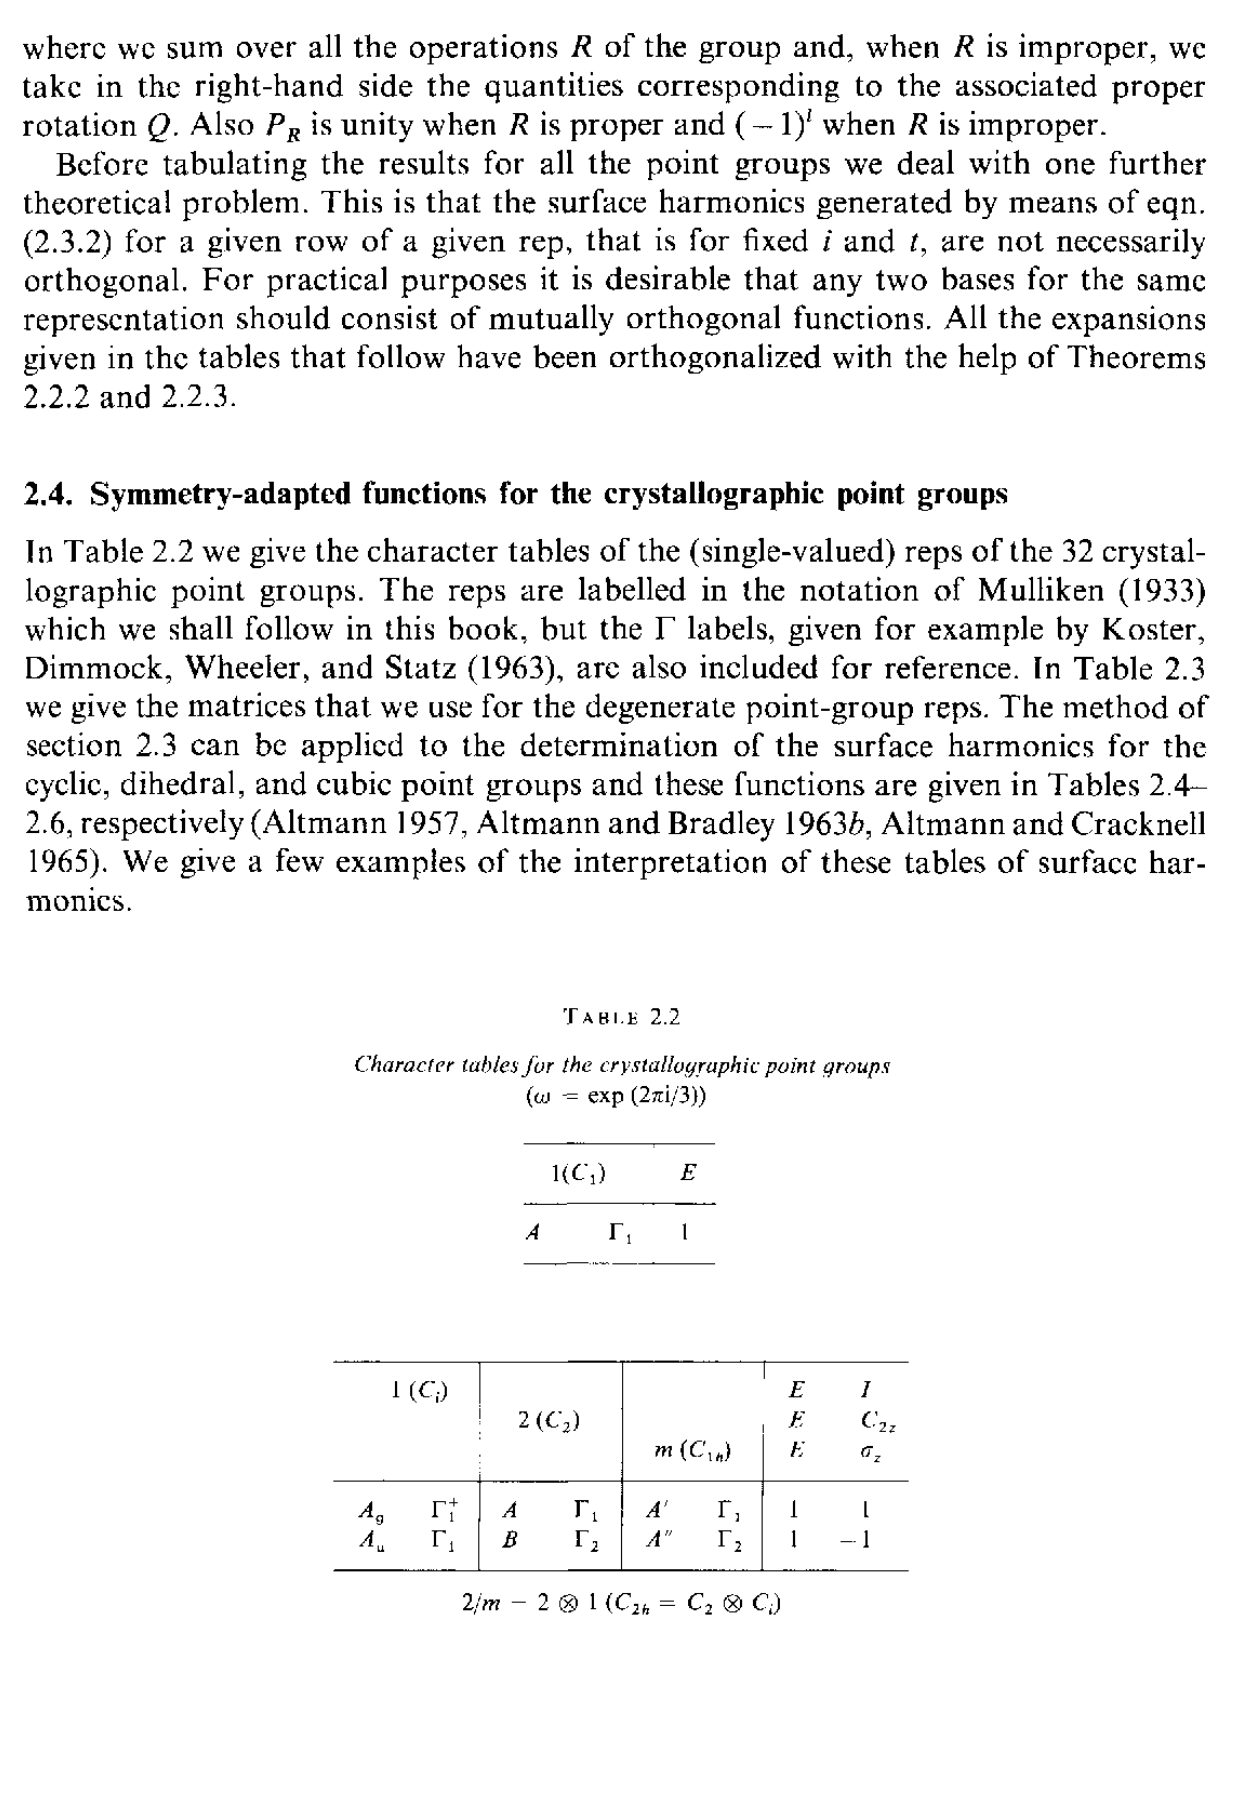
\includegraphics[width=0.86\textwidth]{c2_t22_p1.png}
\caption*{表 2.2（第一部分）：$1\ (C_{1})$、$\bar{1}\ (C_{i})$、$2\ (C_{2})$、$m\ (C_{1h})$、$mm2\ (C_{2v})$、$222\ (D_{2})$、$2/m\ (C_{2h})$ 的特征标表（原书扫描占位）。}
\end{figure}
\begin{figure}[H]
\centering
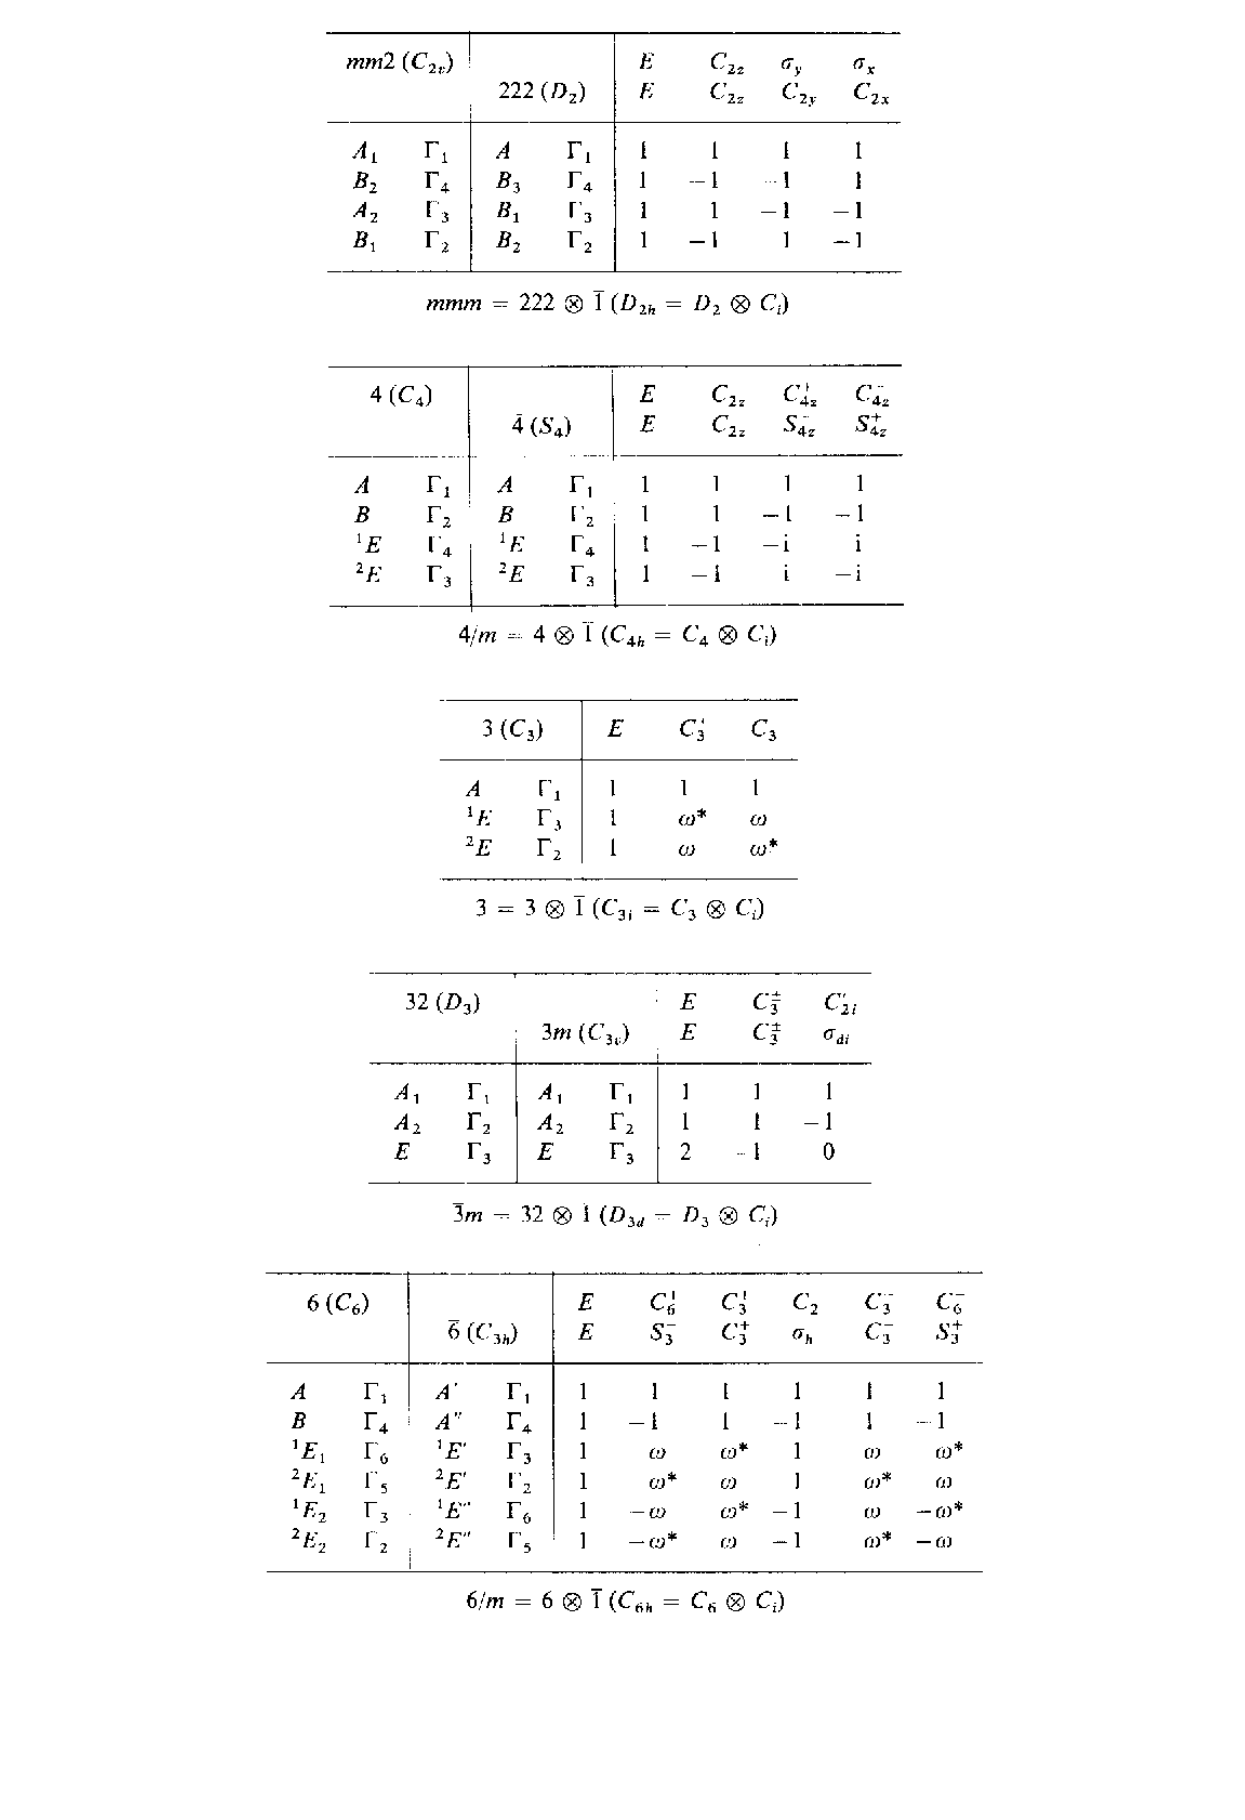
\includegraphics[width=0.86\textwidth]{c2_t22_p2.png}
\caption*{表 2.2（第二部分）：$4\ (C_{4})$、$\bar{4}\ (S_{4})$、$4/m\ (C_{4h})$、$3\ (C_{3})$、$\bar{3}\ (C_{3i})$、$32\ (D_{3})$、$3m\ (C_{3v})$、$\bar{3}m\ (D_{3d})$、$6\ (C_{6})$、$\bar{6}\ (C_{3h})$、$6/m\ (C_{6h})$ 的特征标表（原书扫描占位）。}
\end{figure}
\begin{figure}[H]
\centering
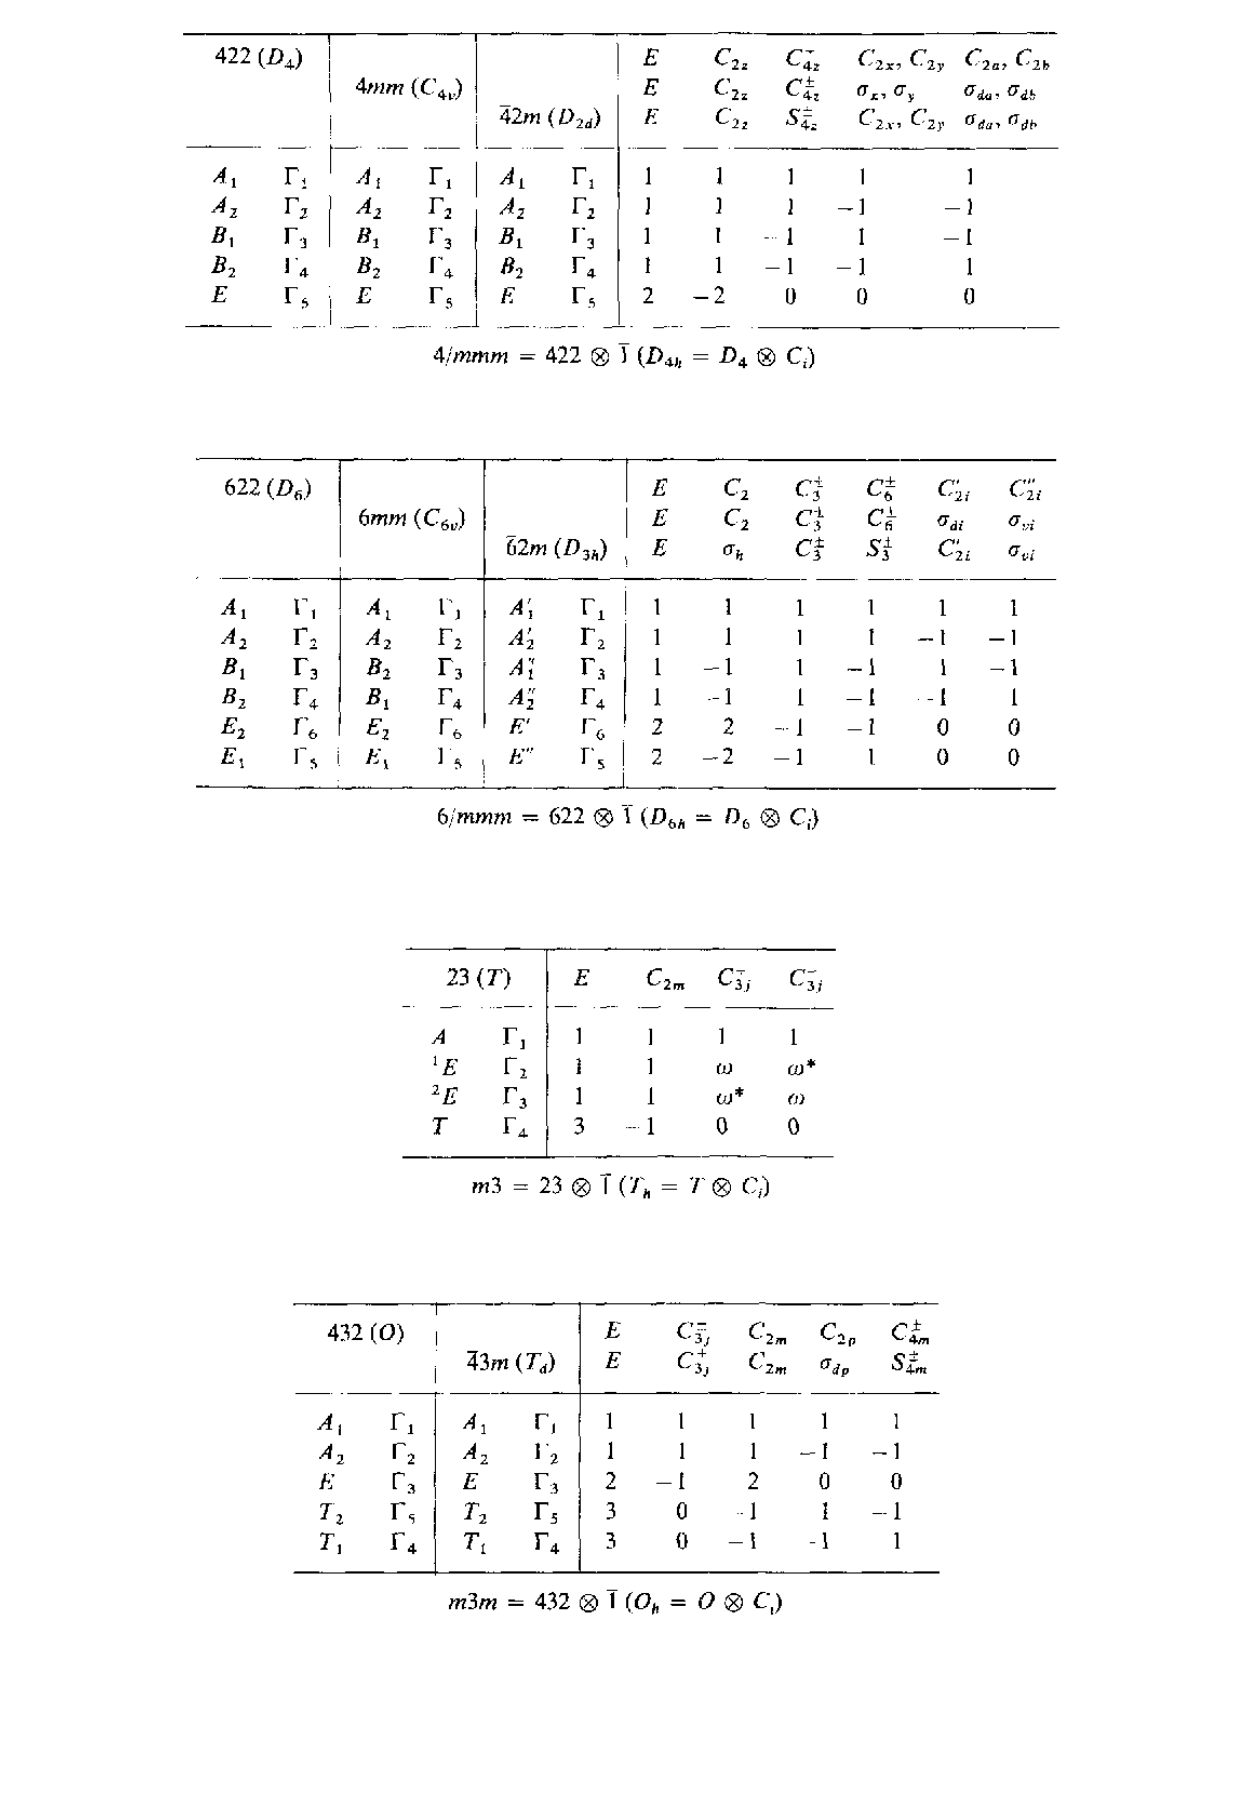
\includegraphics[width=0.86\textwidth]{c2_t22_p3.png}
\caption*{表 2.2（第三部分）：$422\ (D_{4})$、$4mm\ (C_{4v})$、$\bar{4}2m\ (D_{2d})$、$4/mmm\ (D_{4h})$、$622\ (D_{6})$、$6mm\ (C_{6v})$、$\bar{6}2m\ (D_{3h})$、$6/mmm\ (D_{6h})$、$23\ (T)$、$m3\ (T_{h})$、$432\ (O)$、$\bar{4}3m\ (T_{d})$、$m3m\ (O_{h})$ 的特征标表，以及表 2.3（简并表示的矩阵）的开头（原书扫描占位）。}
\end{figure}
\begin{figure}[H]
\centering
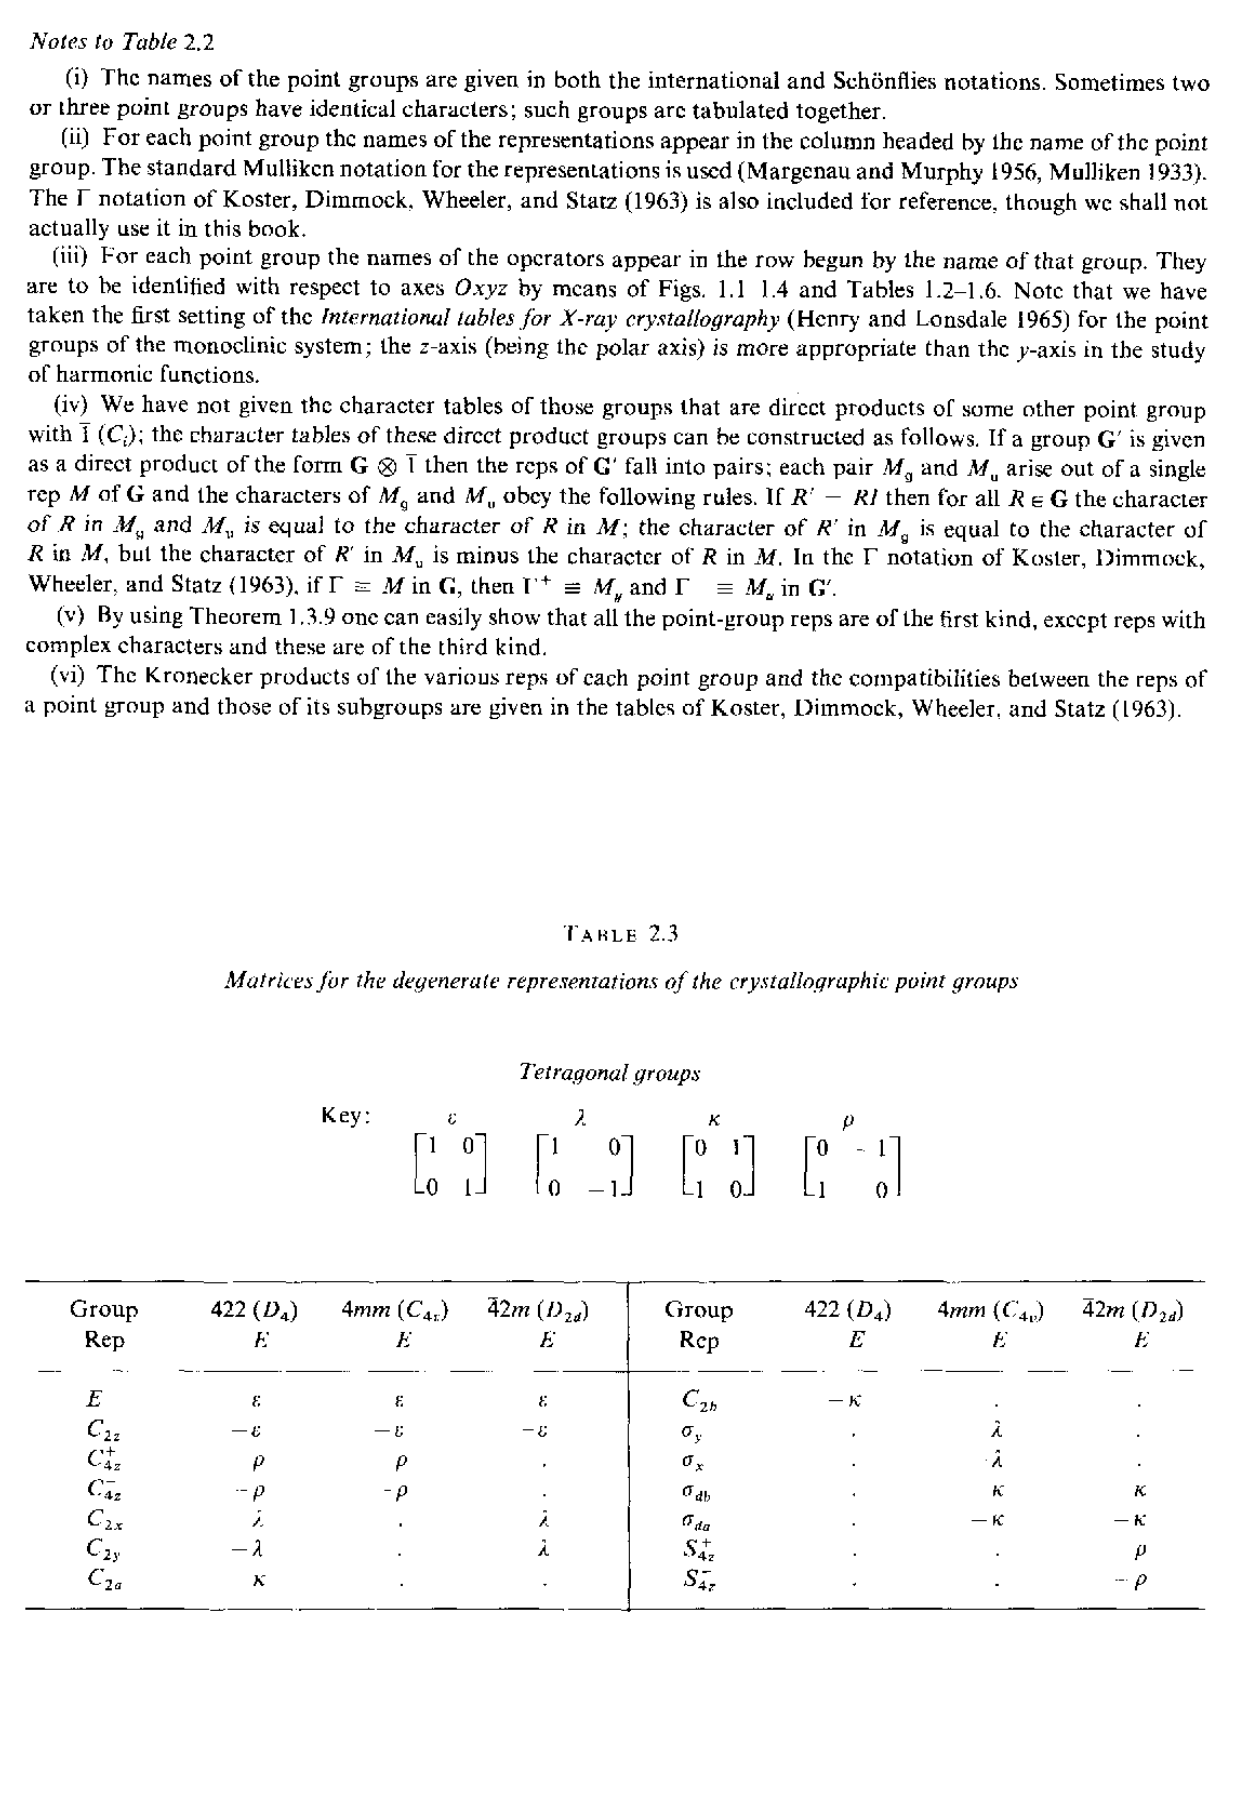
\includegraphics[width=0.86\textwidth]{c2_t23.png}
\caption*{表 2.3（续）：四方群、三方与六方群简并表示的矩阵（原书扫描占位）。}
\end{figure}
\begin{figure}[H]
\centering
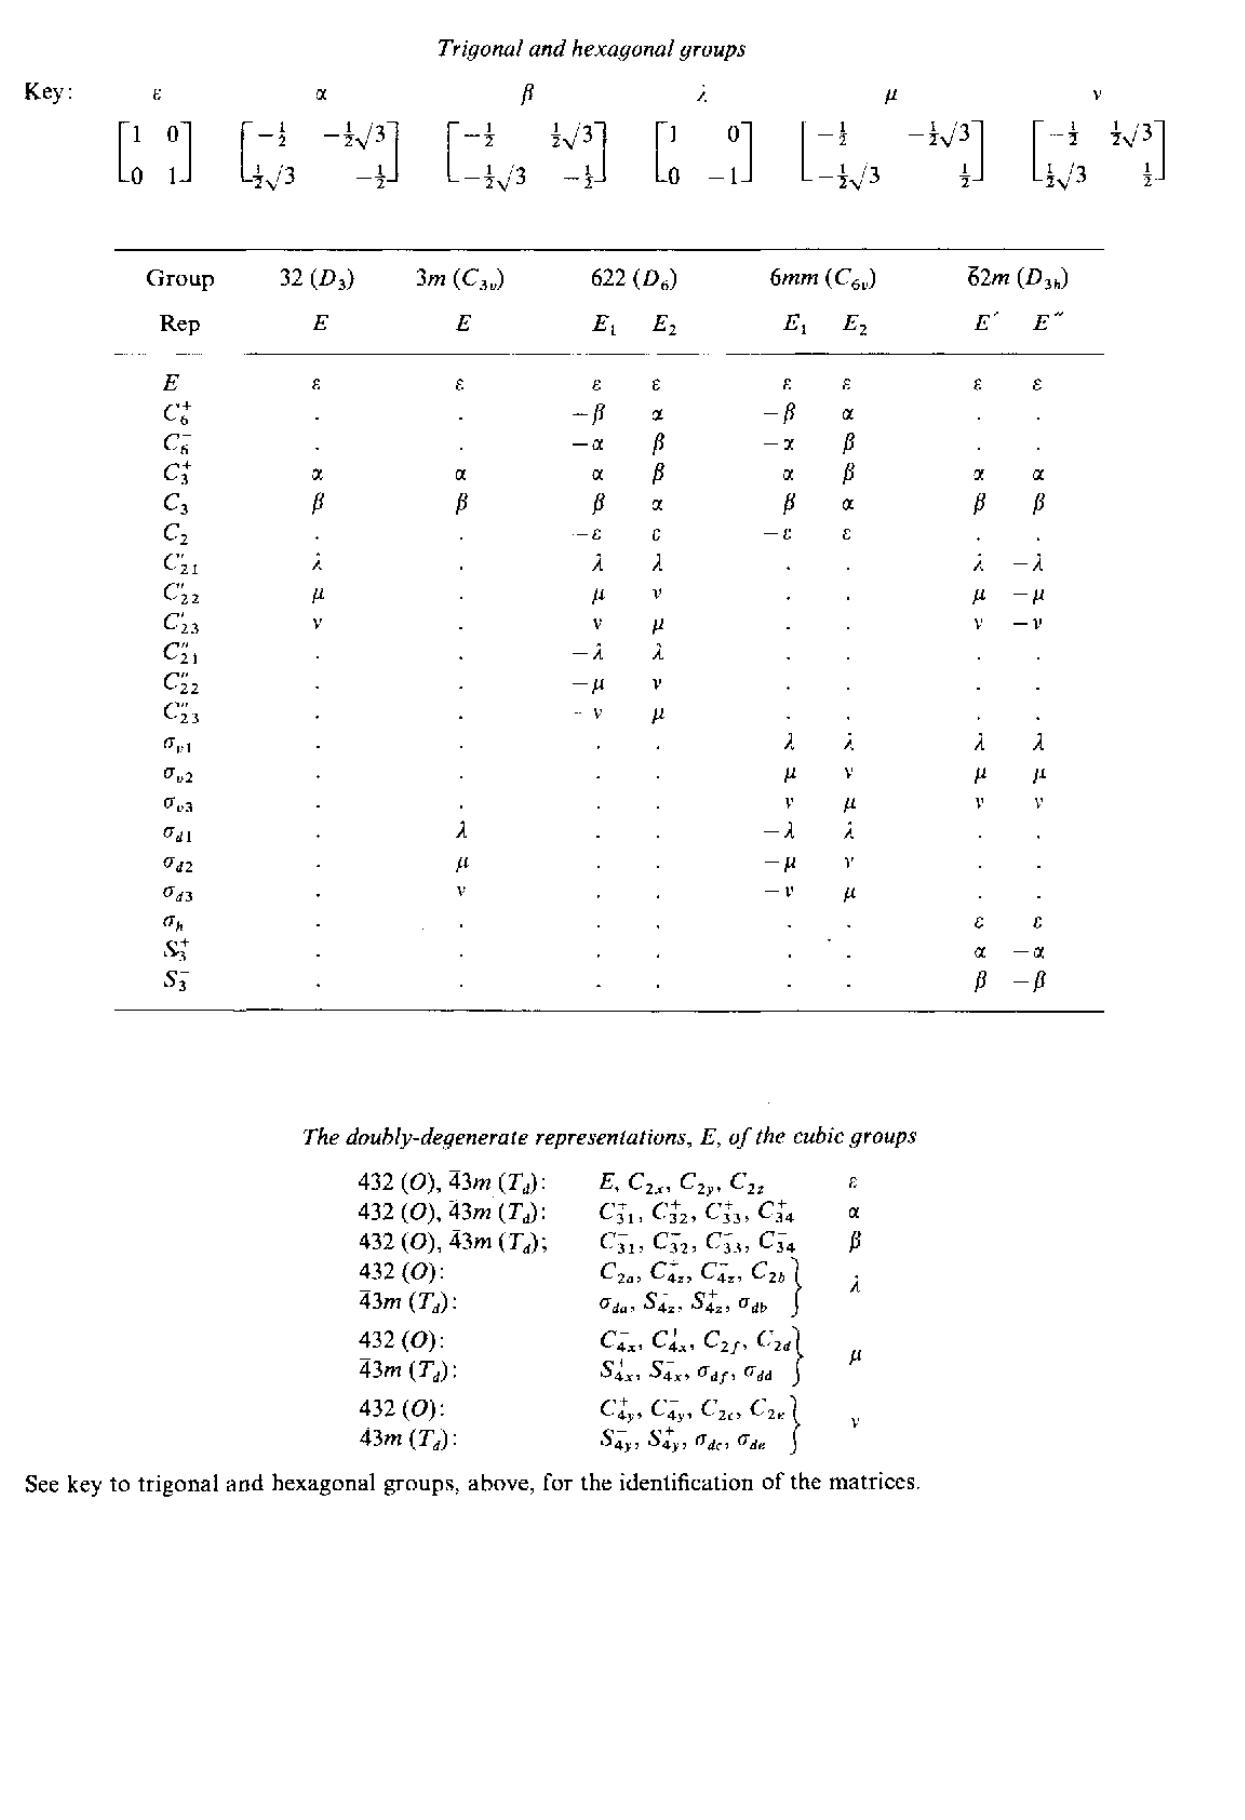
\includegraphics[width=0.86\textwidth]{c2_t24_t25.png}
\caption*{表 2.3（续）：三方与六方群的矩阵 Key，以及立方群二重简并表示 $E$ 的矩阵（原书扫描占位）。}
\end{figure}
\begin{figure}[H]
\centering
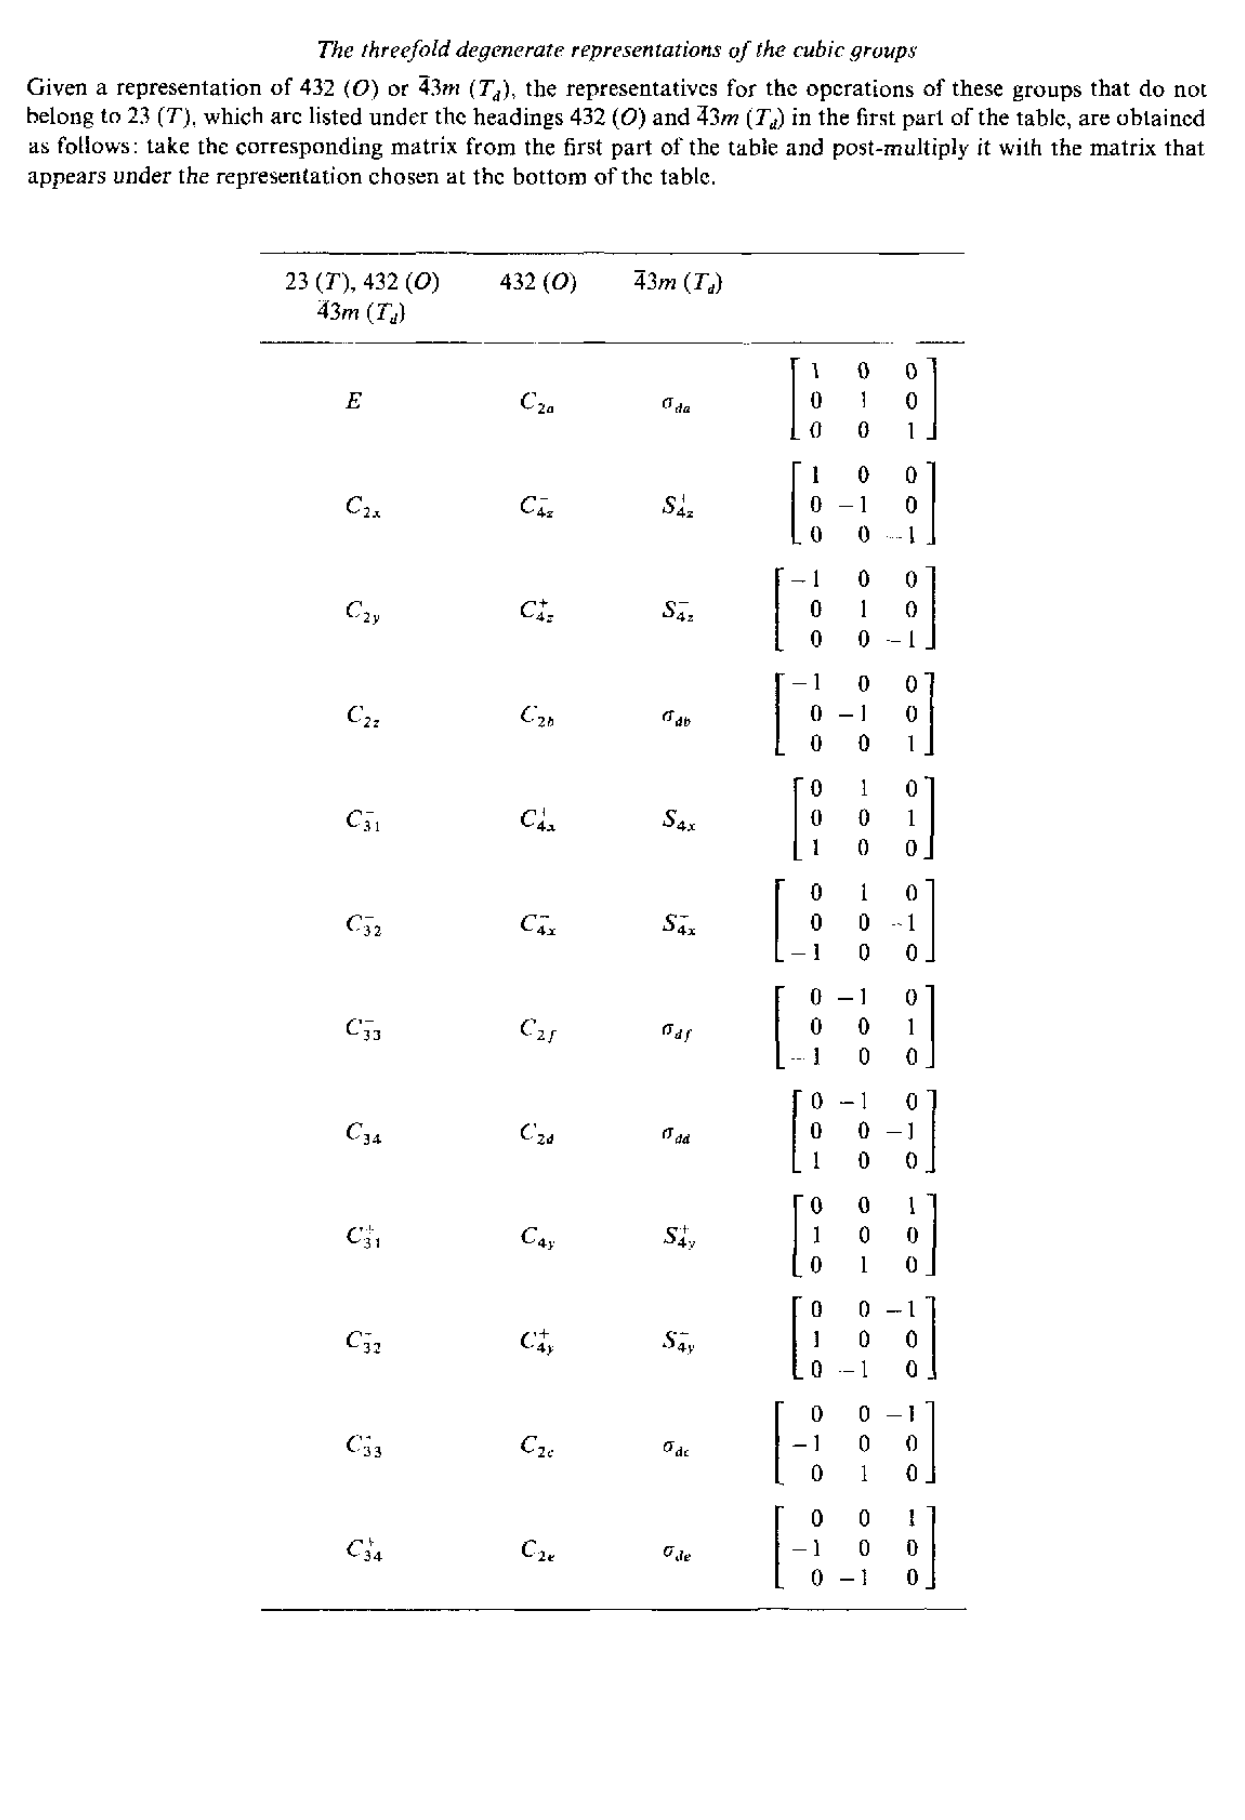
\includegraphics[width=0.86\textwidth]{c2_t25_t26.png}
\caption*{表 2.3（结尾）与表 2.4（循环群的面谐函数）开头（原书扫描占位）。}
\end{figure}
\begin{figure}[H]
\centering
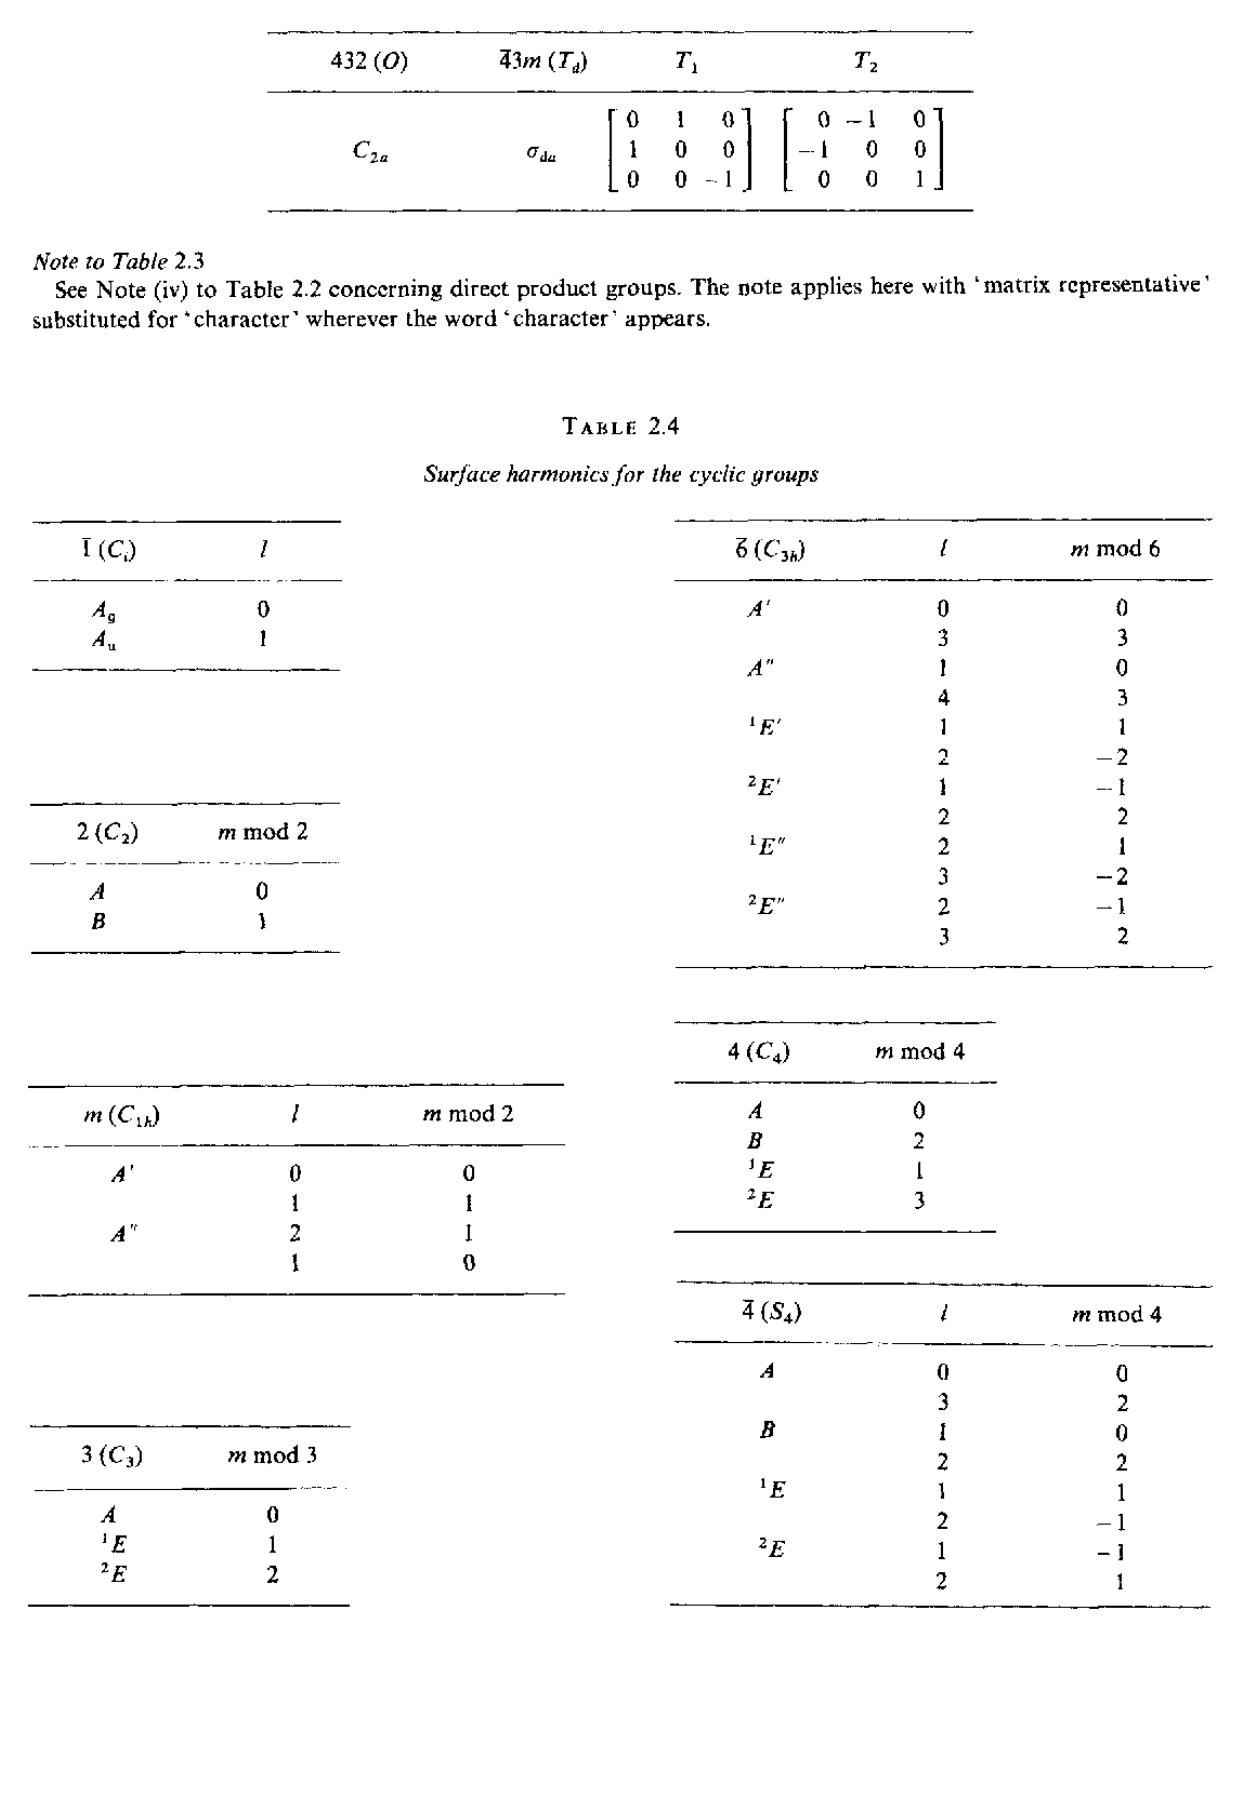
\includegraphics[width=0.86\textwidth]{c2_t26.png}
\caption*{表 2.4（续）：循环群的面谐函数（原书扫描占位）。}
\end{figure}
\begin{figure}[H]
\centering
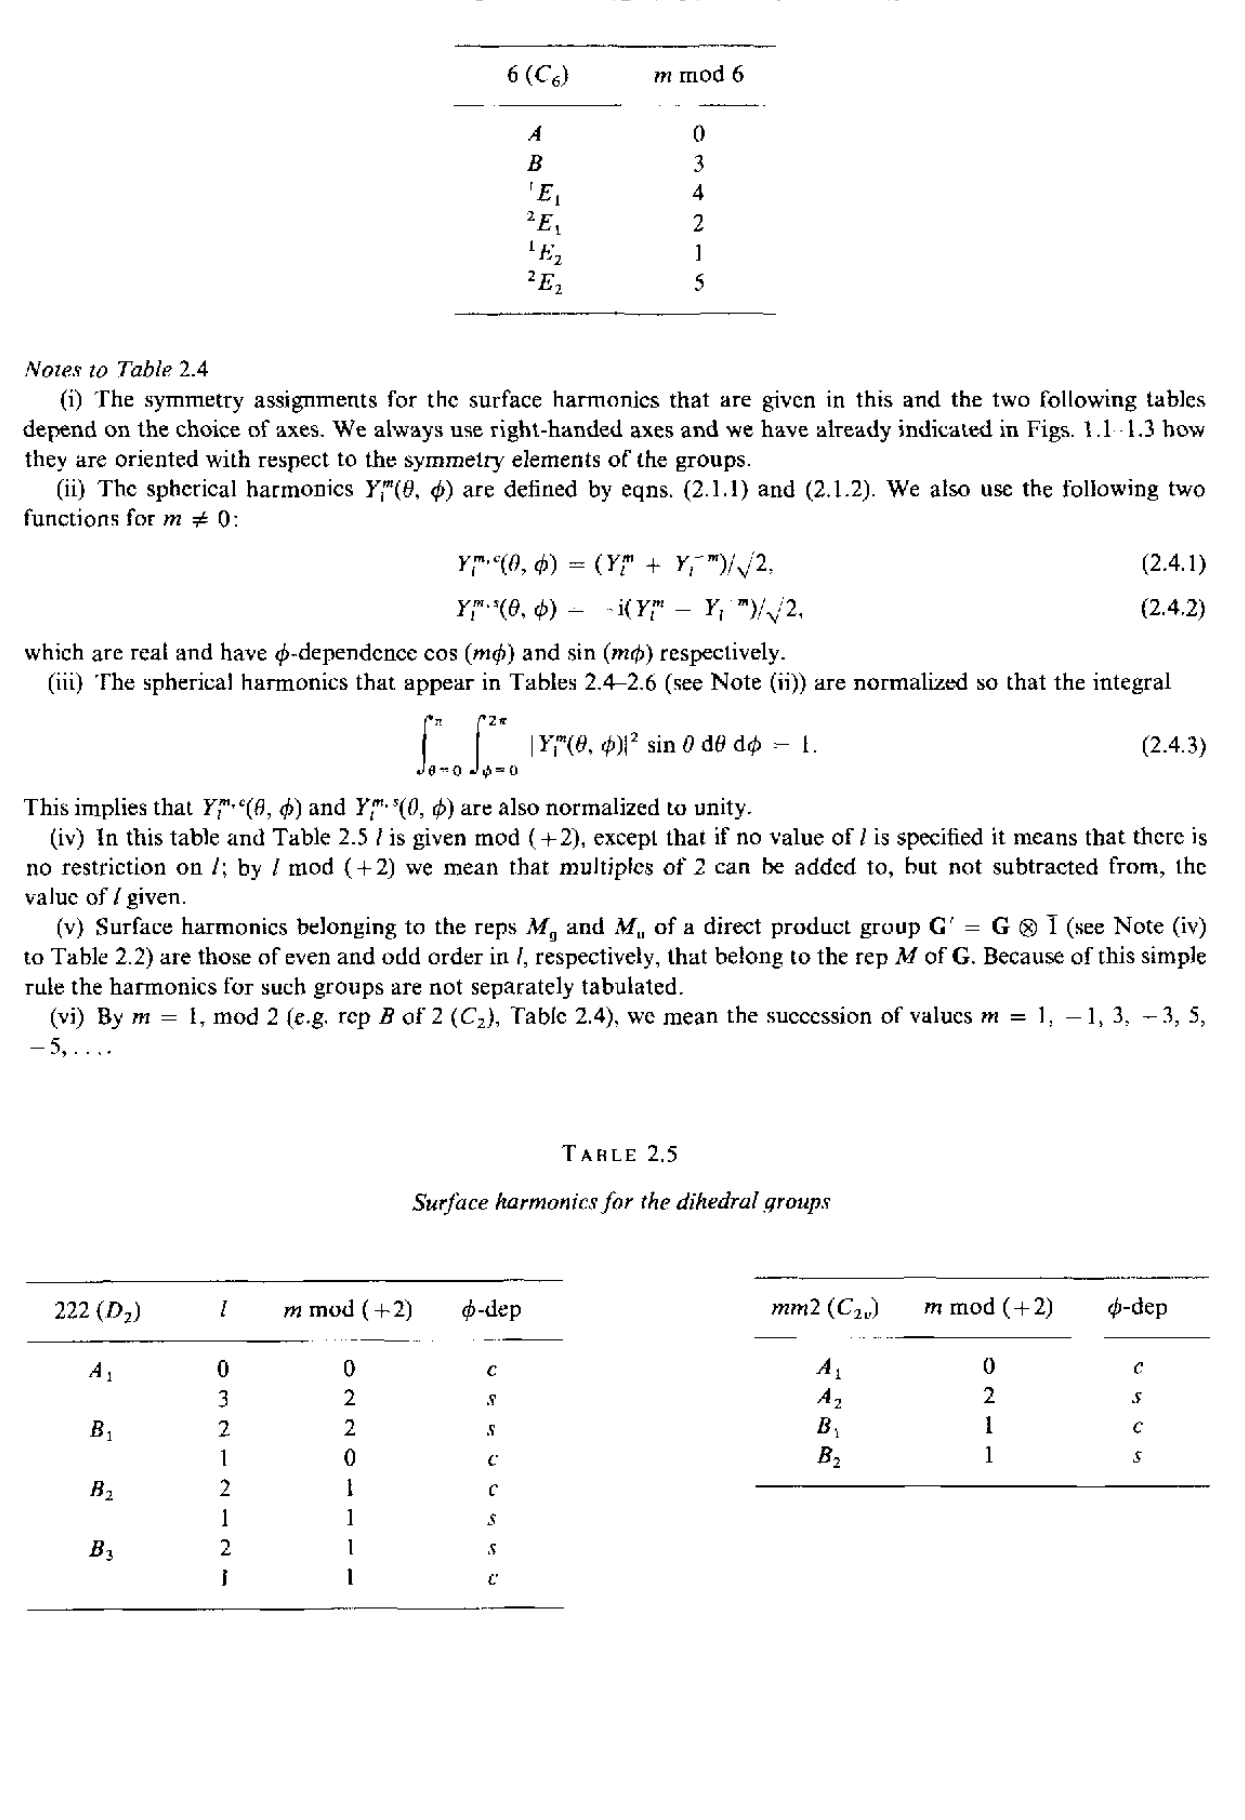
\includegraphics[width=0.86\textwidth]{c2_t27_p1.png}
\caption*{表 2.4（结尾）及其注，与表 2.5（二面体群的面谐函数）（原书扫描占位）。}
\end{figure}
\begin{figure}[H]
\centering
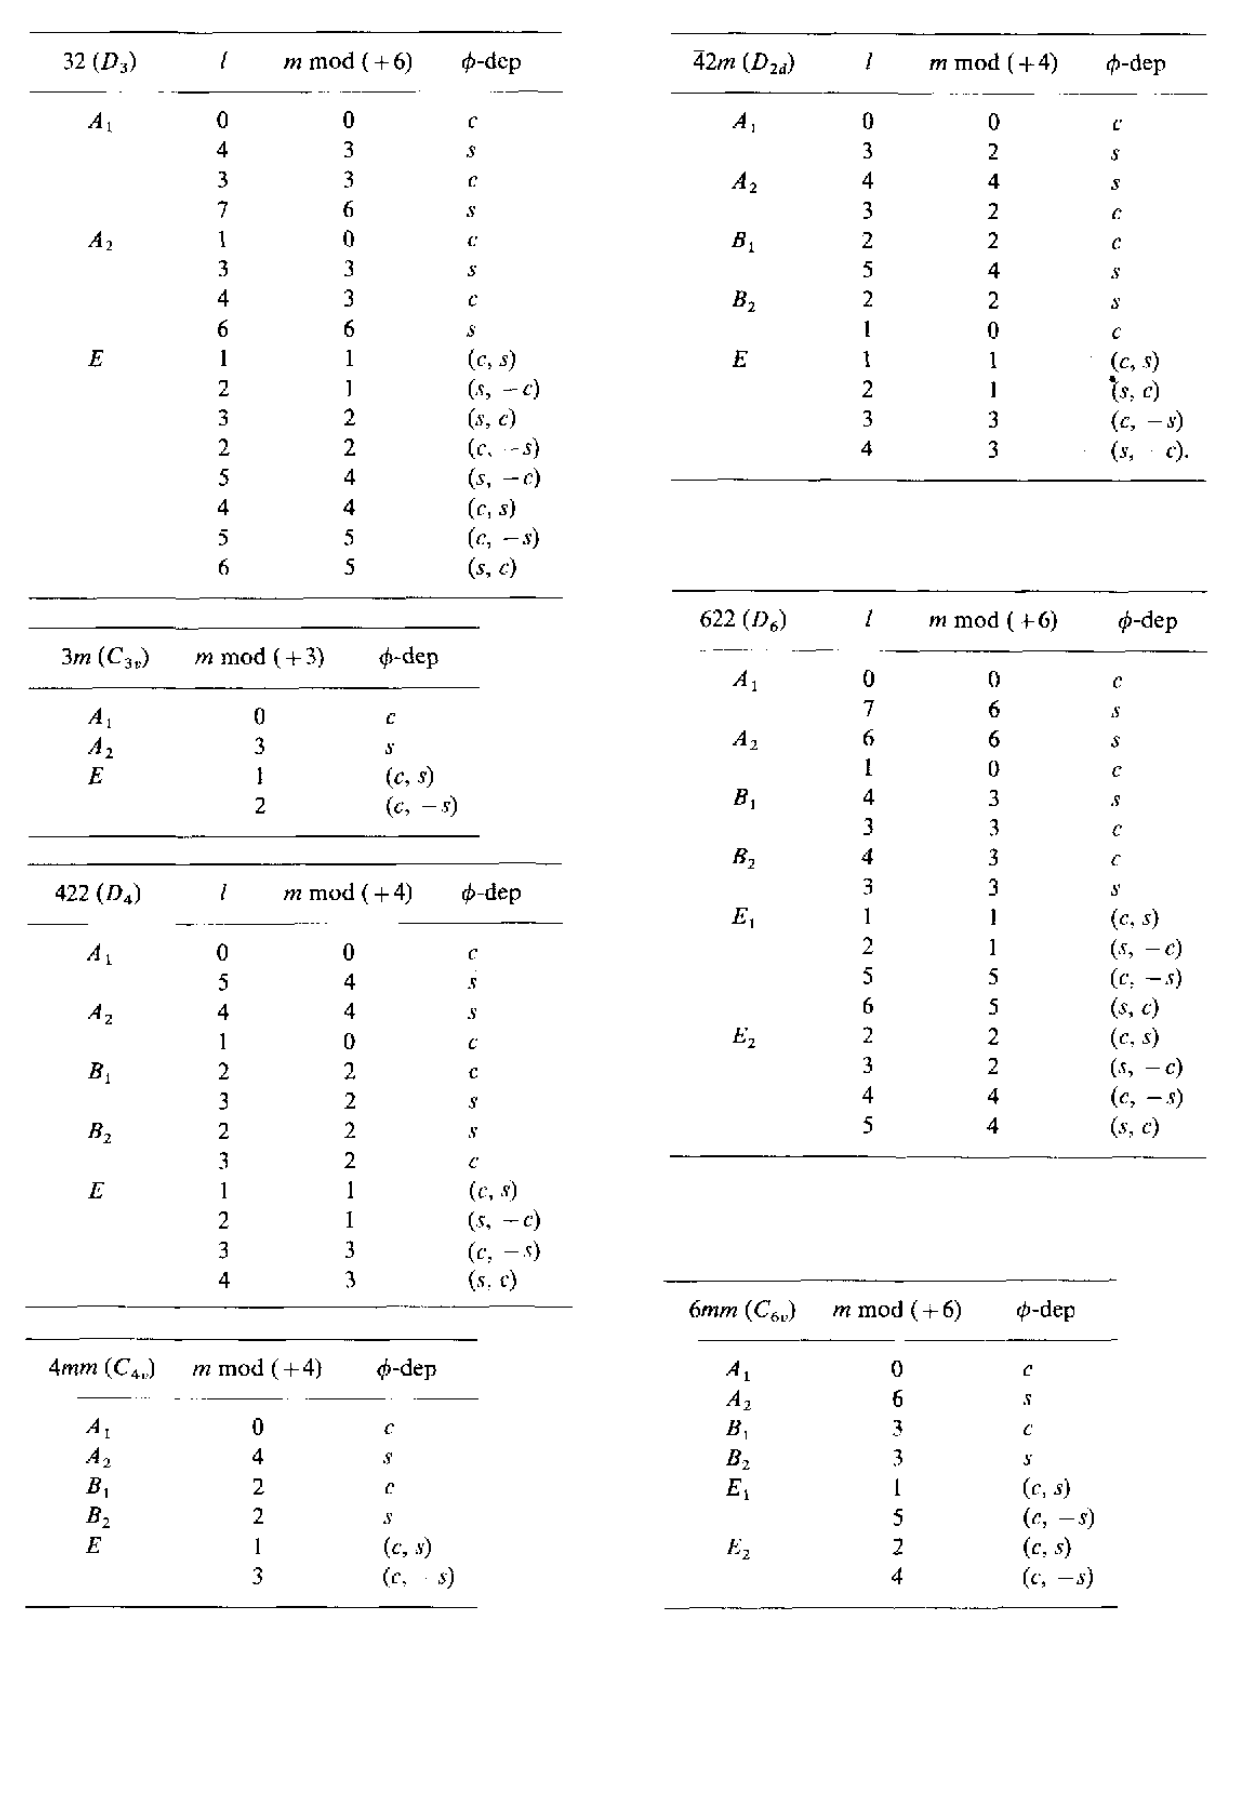
\includegraphics[width=0.86\textwidth]{c2_t27_p2.png}
\caption*{表 2.5（续）与表 2.6 的开头：三方、六方及立方群的面谐函数（原书扫描占位）。}
\end{figure}
\begin{figure}[H]
\centering
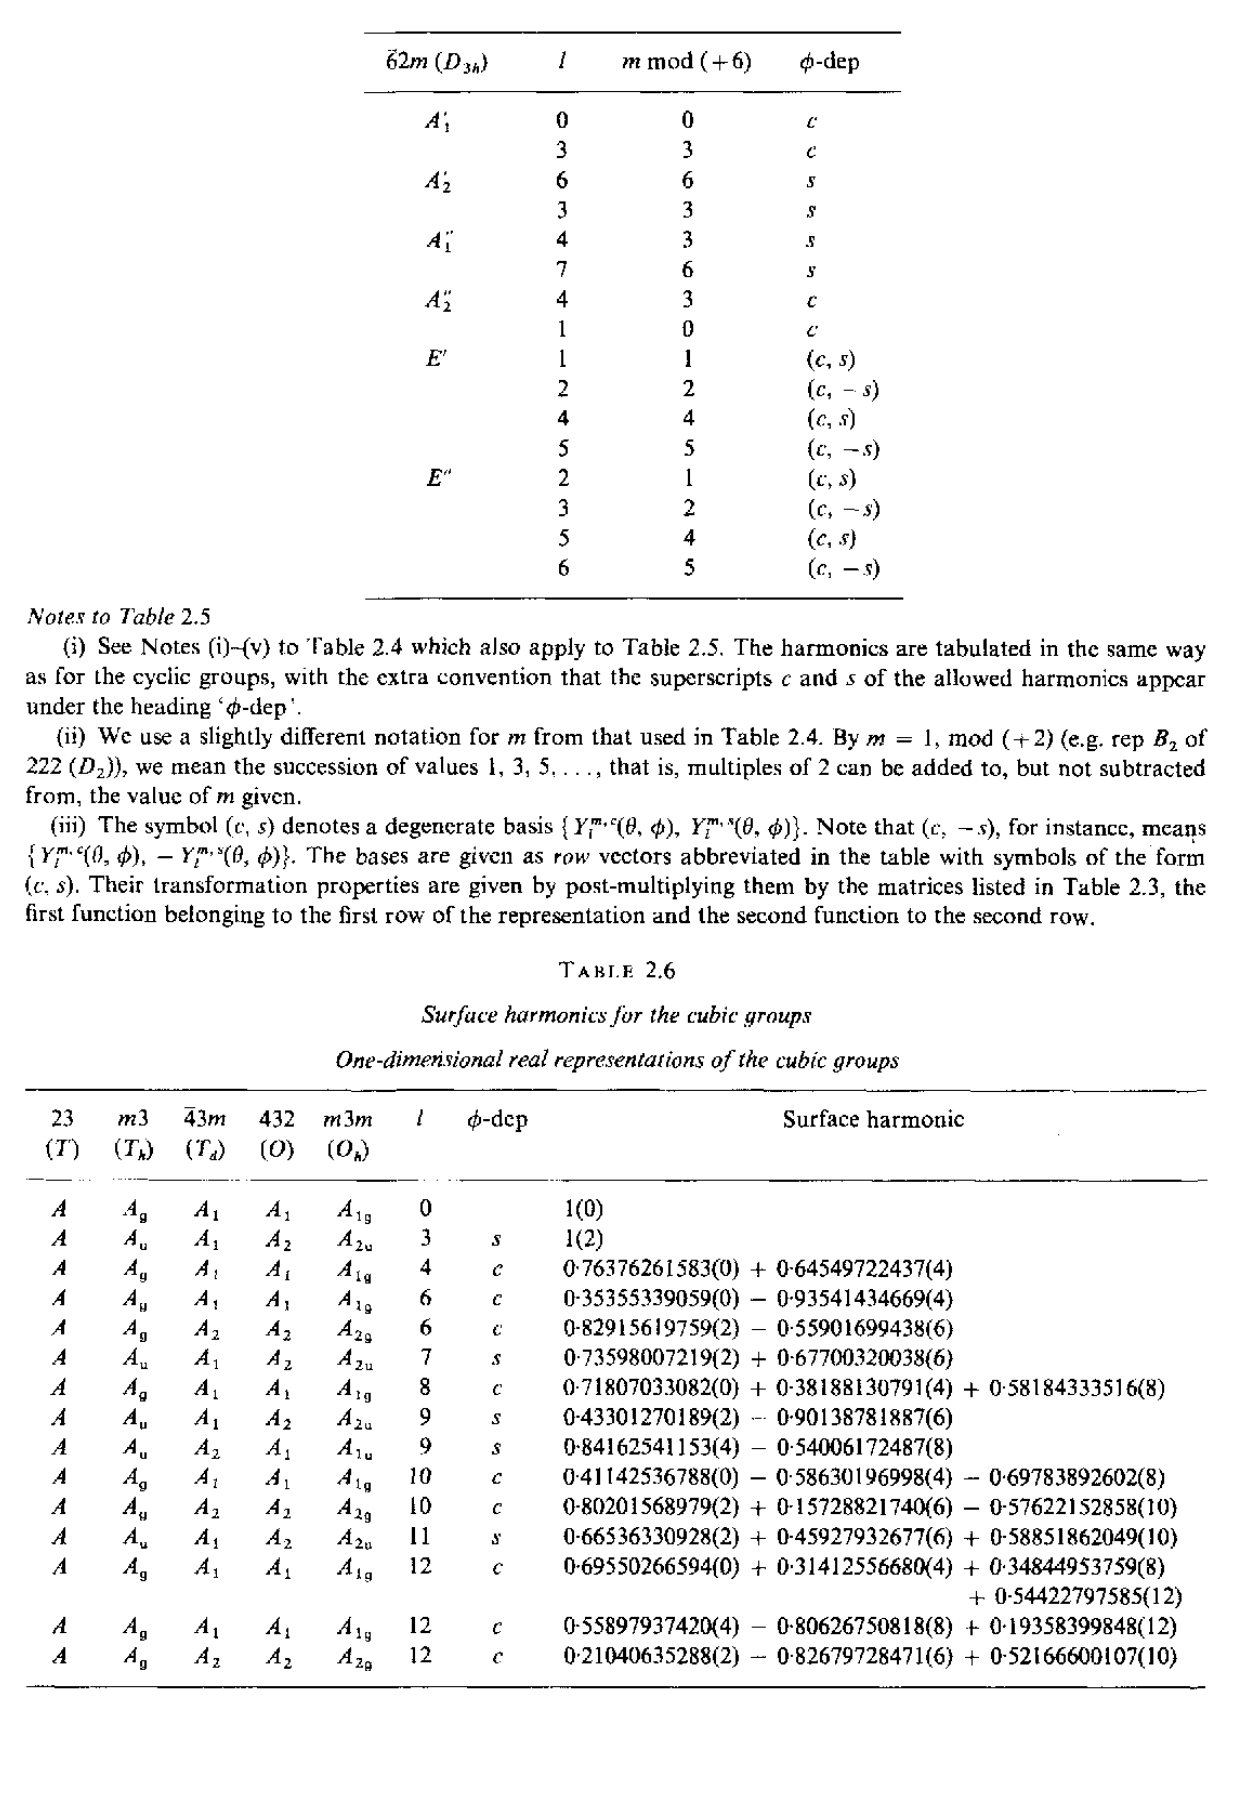
\includegraphics[width=0.86\textwidth]{c2_t27_p3.png}
\caption*{表 2.6（续）：立方群与三方、六方群的面谐函数（原书扫描占位）。}
\end{figure}
\begin{figure}[H]
\centering
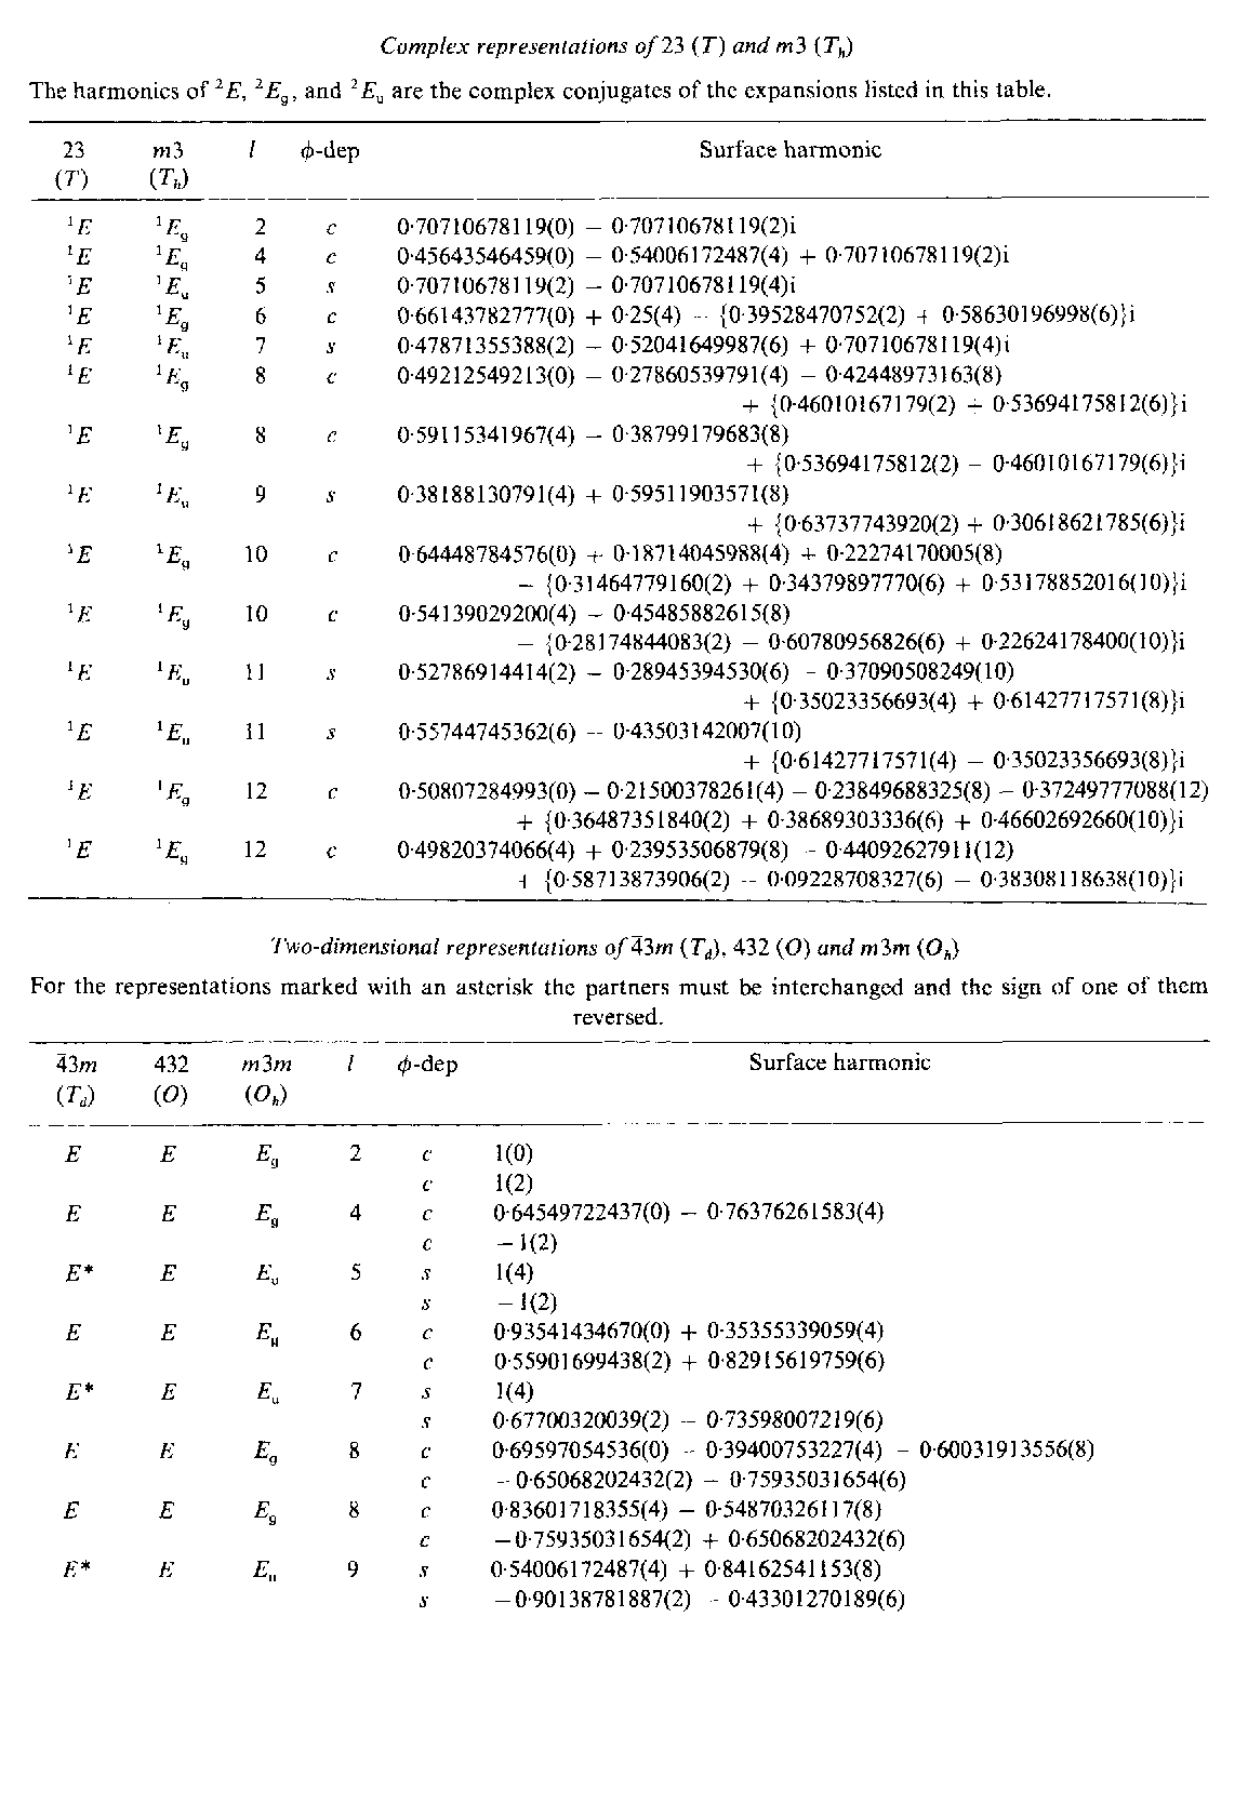
\includegraphics[width=0.86\textwidth]{c2_t27_p4.png}
\caption*{表 2.7：$O(3)$ 的表示 $\mathscr{D}^{l}$ 与点群表示的相容表（第一部分，原书扫描占位）。}
\end{figure}
\begin{figure}[H]
\centering
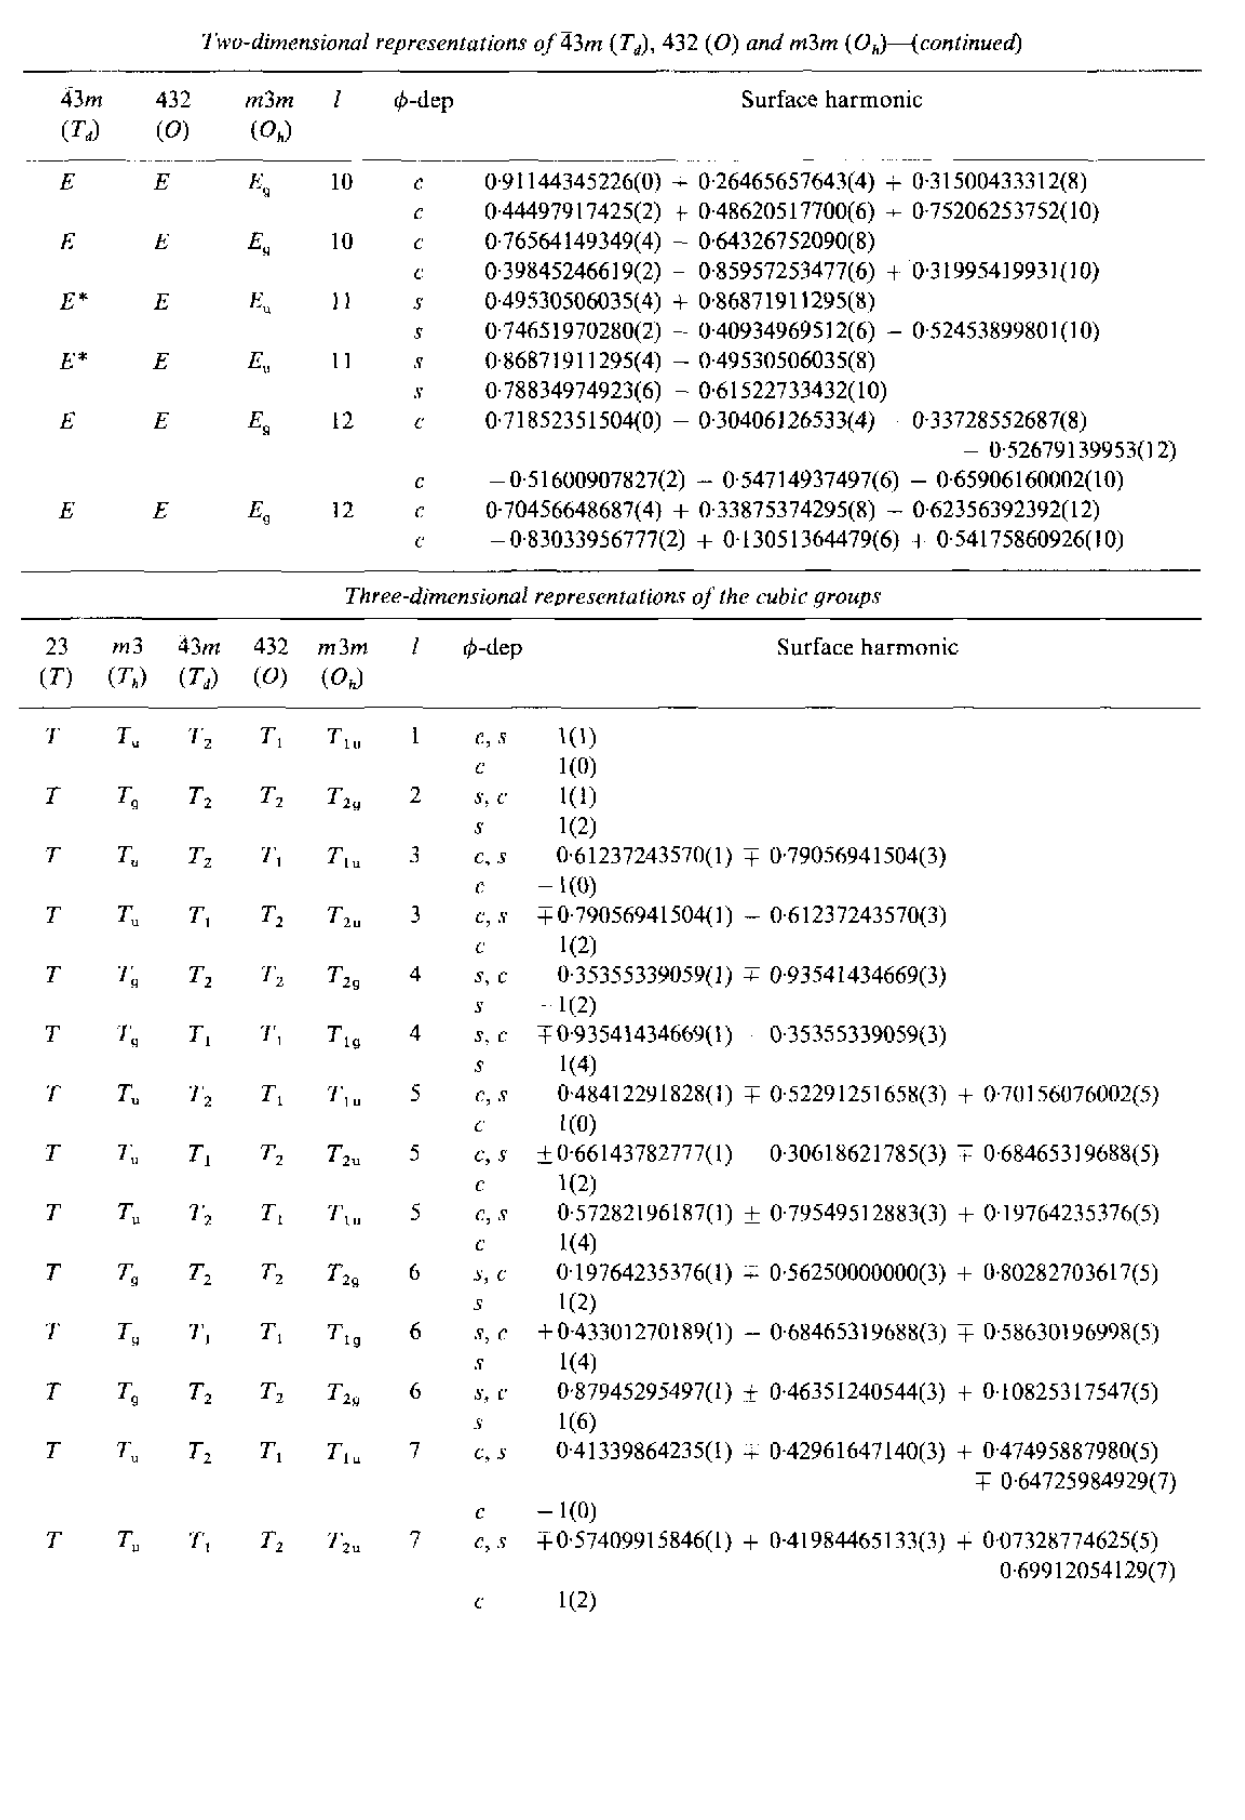
\includegraphics[width=0.86\textwidth]{c2_t27_p5.png}
\caption*{表 2.7（第二部分，原书扫描占位）。}
\end{figure}
\begin{figure}[H]
\centering
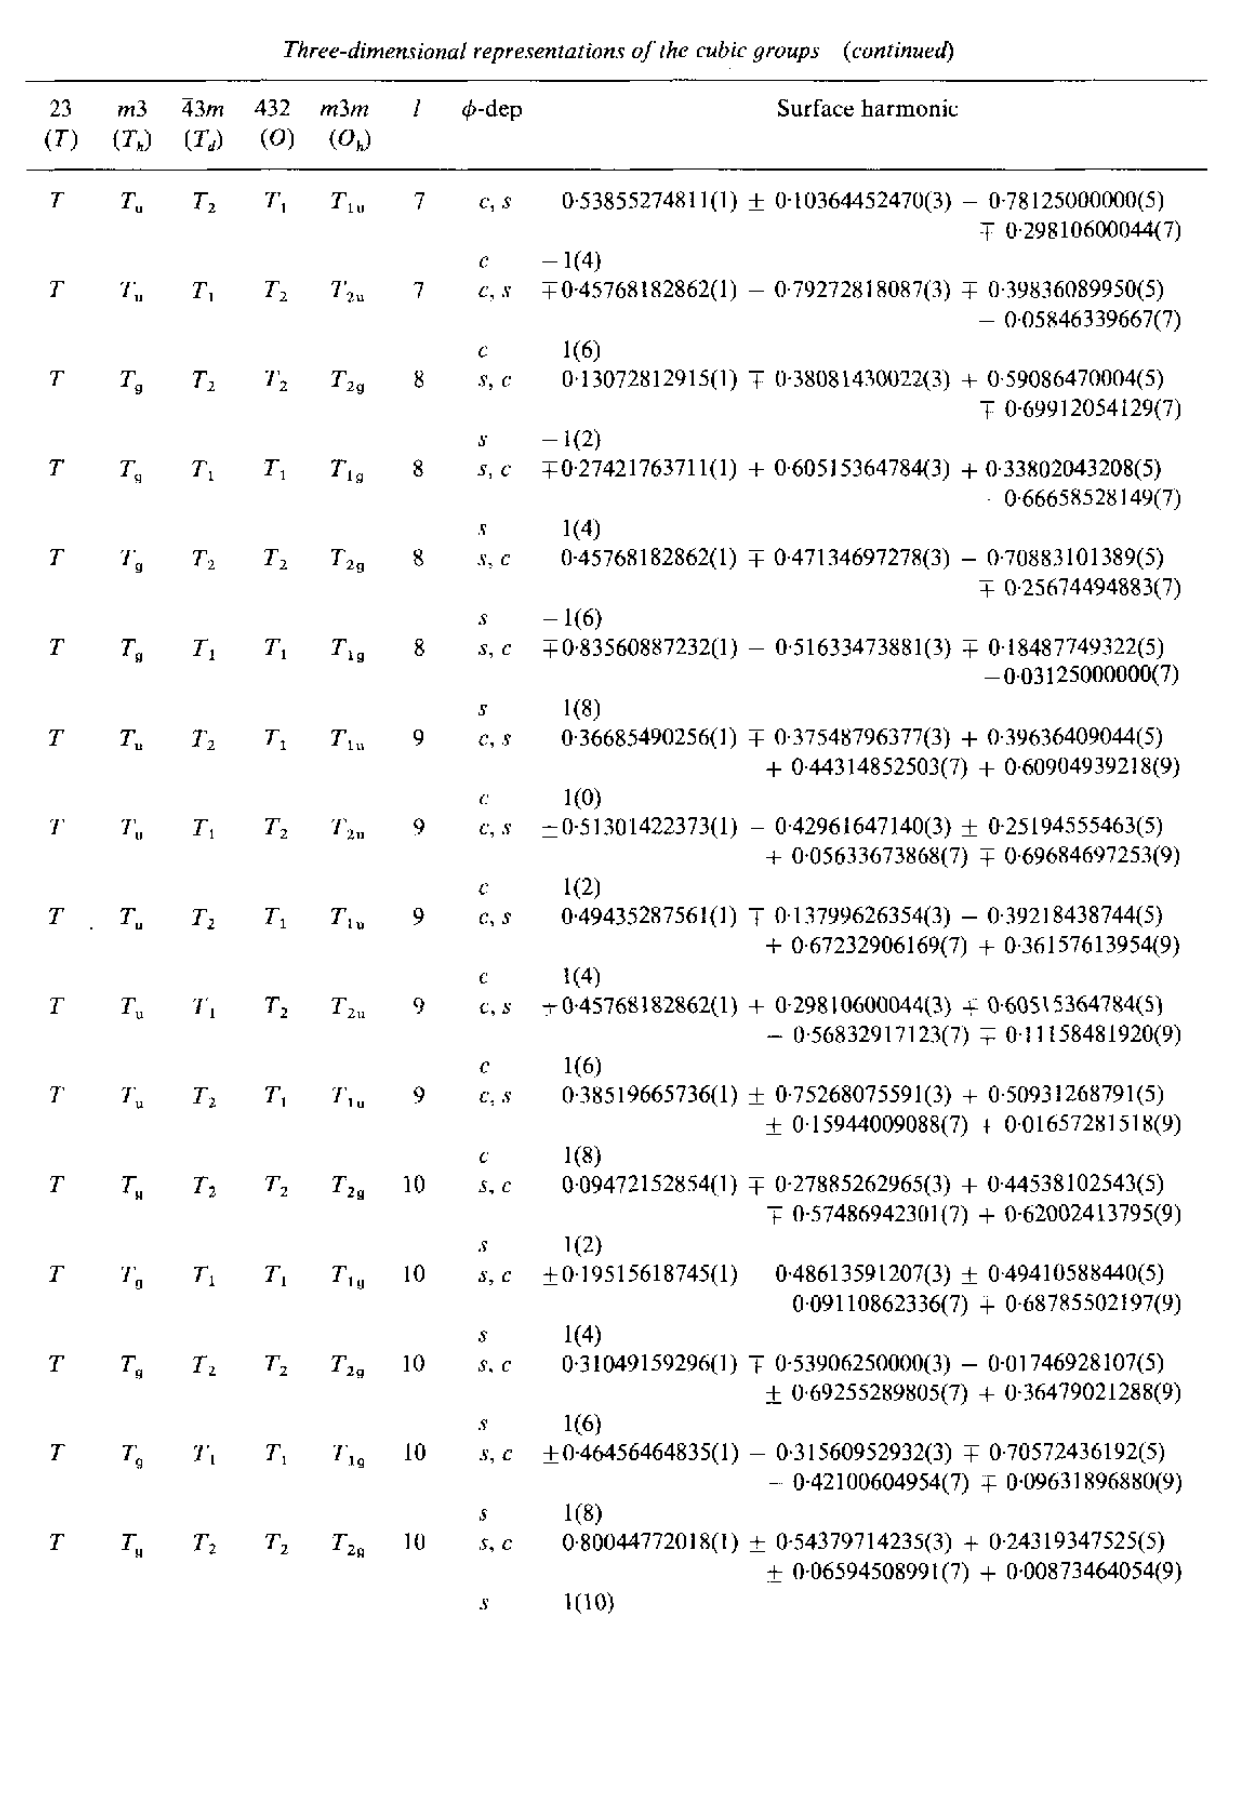
\includegraphics[width=0.86\textwidth]{c2_t27_p6.png}
\caption*{表 2.7（第三部分，原书扫描占位）。}
\end{figure}


\textit{例} 2.4.3. 取 $l = 2$（即五重简并的原子 D 项），点群 $mm2$（$C_{2v}$）为 $\mathbf{G}$。按表 2.7，该项在 $mm2$（$C_{2v}$）中劈裂为五个非简并能级：

\begin{equation*}
\mathscr{D}^{2}\{R(\alpha, \beta, \gamma)\} = 2A_{1} + A_{2} + B_{1} + B_{2}.
\tag{2.4.4}
\end{equation*}

$\mathscr{D}^{2}\{R(\alpha, \beta, \gamma)\}$ 的基函数是 $\{Y_{2}^{-2}(\theta, \phi), Y_{2}^{-1}(\theta, \phi), Y_{2}^{0}(\theta, \phi), Y_{2}^{1}(\theta, \phi), Y_{2}^{2}(\theta, \phi)\}$；由表 2.5 可见，这些函数按式 (2.4.4) 分配到 $mm2$（$C_{2v}$）的五个表示：$A_{1}$：$Y_{2}^{0}(\theta, \phi)$，$Y_{2}^{2,c}(\theta, \phi)$；$A_{2}$：$Y_{2}^{2,s}(\theta, \phi)$；$B_{1}$：$Y_{2}^{1,c}(\theta, \phi)$；$B_{2}$：$Y_{2}^{1,s}(\theta, \phi)$。见图 2.2。

\begin{figure}[H]
\centering
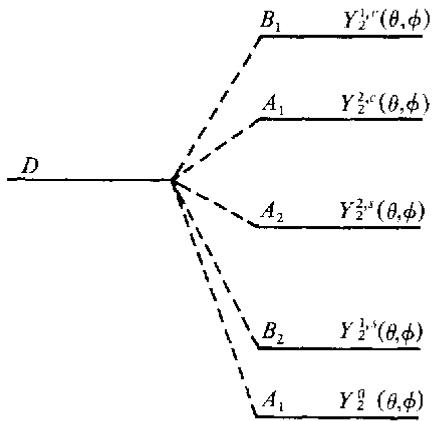
\includegraphics[width=0.46\textwidth]{fig2_2_mu.jpg}
\caption{原子 D 项在具有 $mm2$（$C_{2v}$）对称性的晶体场中的示意劈裂。}
\end{figure}

\textit{例} 2.4.4. 作为第二个例子，取 $l = 3$（即七重简并的原子 F 项），点群取立方群 432（$O$）。按表 2.7 有

\begin{equation*}
\mathscr{D}^{3}\{R(\alpha, \beta, \gamma)\} = A_{2} + T_{1} + T_{2}.
\tag{2.4.5}
\end{equation*}

$A_{2}$ 是 432（$O$）的非简并表示，$T_{1}$ 与 $T_{2}$ 是 432（$O$）的三重简并表示。与这些能级对应的波函数角部分是 $Y_{3}^{0}(\theta, \phi)$，$Y_{3}^{1,c}(\theta, \phi)$，$Y_{3}^{1,s}(\theta, \phi)$，$Y_{3}^{2,c}(\theta, \phi)$，$Y_{3}^{2,s}(\theta, \phi)$，$Y_{3}^{3,c}(\theta, \phi)$，$Y_{3}^{3,s}(\theta, \phi)$ 的线性组合。由表 2.6：属于 $A_{2}$ 的面谐函数为 $Y_{3}^{2,s}(\theta, \phi)$；属于 $T_{1}$ 的为 $[\{aY_{3}^{1,c}(\theta, \phi) - bY_{3}^{3,c}(\theta, \phi)\}, \{aY_{3}^{1,s}(\theta, \phi) + bY_{3}^{3,s}(\theta, \phi)\}, \{-Y_{3}^{0}(\theta, \phi)\}]$；属于 $T_{2}$ 的为 $[\{-bY_{3}^{1,c}(\theta, \phi) - aY_{3}^{3,c}(\theta, \phi)\}, \{bY_{3}^{1,s}(\theta, \phi) - aY_{3}^{3,s}(\theta, \phi)\}, \{Y_{3}^{2,c}(\theta, \phi)\}]$，其中 $a = 0.612\,372\,435\,7$，$b = 0.790\,569\,415\,0$。原子 F 项在 432（$O$）晶体场中的劈裂见图 2.3。

\begin{figure}[H]
\centering
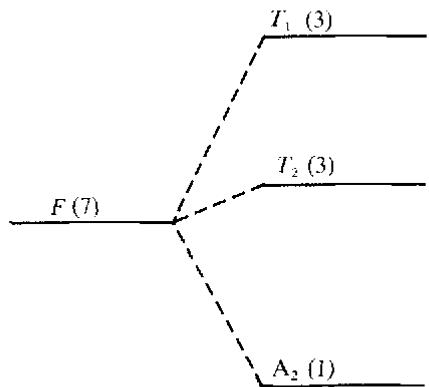
\includegraphics[width=0.46\textwidth]{fig2_3_mu.jpg}
\caption{原子 F 项在具有 432（$O$）对称性的晶体场中的示意劈裂（括号内给出各能级的简并度）。}
\end{figure}

% 2.5 主动与被动算符；2.6 表示的对称化与反对称化乘积
\section{主动与被动算符}

为完整起见，这里说明由主动操作构成的群的表示的基函数与相应被动操作群的表示之间的关系。

设 $X, Y, Z, \ldots$ 是一群算符（例如点群操作），按主动形式考虑时有 $X_{a}Y_{a} = Z_{a}$。再设已给定这些主动操作的一个表示 $\Gamma_{a}^{i}$，使得 $\mathbf{D}_{a}^{i}(X_{a})\mathbf{D}_{a}^{i}(Y_{a}) = \mathbf{D}_{a}^{i}(Z_{a})$，基函数记为 $\langle \phi_{t}^{i}|$，例如

\begin{equation*}
\bar{X}_{a}\phi_{t}^{i} = \sum_{j} \phi_{j}^{i}\mathbf{D}_{a}^{i}(X_{a})_{jt},
\tag{2.5.1}
\end{equation*}

其中 $\bar{X}_{a}$ 是主动函数空间算符（见 1.5 节）。现在若想使用被动形式的算符：首先 $X_{p} = X_{a}^{-1}$，故群的乘法表有所不同，例如此时有 $Y_{p}X_{p} = Z_{p}$。群当然是同一个群；乘法不同是因为把元素映到其逆的映射是一个反自同构。

\textbf{定理 2.5.1.} \textit{若 $\langle \phi_{t}^{i}|$ 是群 $\mathbf{G}$ 的元素 $X_{a}, Y_{a}, Z_{a}, \ldots$ 的表示 $\Gamma_{a}^{i}$ 的基，则令 $\mathbf{D}_{p}^{i}(X_{p}) = \mathbf{D}_{a}^{i}(X_{a}^{-1})$，$\langle \phi_{t}^{i}|$ 也是元素 $X_{p} = X_{a}^{-1}, Y_{p} = Y_{a}^{-1}, Z_{p} = Z_{a}^{-1}, \ldots$ 的表示 $\Gamma_{p}^{i}$ 的基。}

这是因为

\begin{equation*}
\bar{X}_{p}\phi_{t}^{i} = \bar{X}_{a}^{-1}\phi_{t}^{i} = \sum_{j} \phi_{j}^{i}\mathbf{D}_{a}^{i}(X_{a}^{-1})_{jt} = \sum_{j} \phi_{j}^{i}\mathbf{D}_{p}^{i}(X_{p})_{jt}
\tag{2.5.2}
\end{equation*}

且

\begin{equation*}
\begin{aligned}
\mathbf{D}_{p}^{i}(Y_{p})\mathbf{D}_{p}^{i}(X_{p}) &= \mathbf{D}_{a}^{i}(Y_{a}^{-1})\mathbf{D}_{a}^{i}(X_{a}^{-1}) = \mathbf{D}_{a}^{i}(Y_{a}^{-1}X_{a}^{-1}) \\
&= \mathbf{D}_{a}^{i}(Z_{a}^{-1}) = \mathbf{D}_{p}^{i}(Z_{p}).
\end{aligned}
\tag{2.5.3}
\end{equation*}

作为这一定理应用的一个例子，考虑本章给出的那些表。本章使用主动算符，并对完整列出的各个矩阵表示给出了基函数。若使用被动算符，则只要把列出的矩阵换成它们的逆，同样的基函数仍然可用。也就是说，我们写 $X$（意为 $X_{a}$）之处你写 $X$（意为 $X_{p}$）；我们的乘法表含 $XY = Z$（意为 $X_{a}Y_{a} = Z_{a}$）之处，你的乘法表含 $YX = Z$（意为 $Y_{p}X_{p} = Z_{p}$）；$\langle \phi_{t}^{i}|$ 是表示 $\Gamma_{p}^{i}$ 的基且 $\mathbf{D}^{i}(Y)\mathbf{D}^{i}(X) = \mathbf{D}^{i}(Z)$（意为 $\mathbf{D}_{p}^{i}(Y_{p})\mathbf{D}_{p}^{i}(X_{p}) = \mathbf{D}_{p}^{i}(Z_{p})$），而我们为表示 $\Gamma_{a}^{i}$ 写下的正是同一组基 $\langle \phi_{t}^{i}|$ 与 $\mathbf{D}^{i}(X)\mathbf{D}^{i}(Y) = \mathbf{D}^{i}(Z)$（意为 $\mathbf{D}_{a}^{i}(X_{a})\mathbf{D}_{a}^{i}(Y_{a}) = \mathbf{D}_{a}^{i}(Z_{a})$）。$\Gamma_{p}^{i}$ 与 $\Gamma_{a}^{i}$ 的矩阵之间的关系是 $\mathbf{D}_{p}^{i}(X) = \mathbf{D}_{a}^{i}(X^{-1}) = \{\mathbf{D}_{a}^{i}(X)\}^{-1}$。最后提醒一句：若 $\mathbf{D}_{a}^{i}(X_{a})$ 与 $\mathbf{D}_{p}^{i}(X_{p})$ 具有不同的特征标，则尽管基函数相同，以 $i$ 标记的表示 $\Gamma_{p}^{i}$ 与 $\Gamma_{a}^{i}$ 在特征标表中将有不同的标记。

\section{点群表示的对称化与反对称化乘积}

作为本章的结束，简要叙述点群表示的对称化与反对称化乘积。这些乘积本身就有重要意义，例如与分子振动（Jahn and Teller 1937）以及二级相变的 Landau 理论（例如见 Birman (1966\textsuperscript{b})，Indenbom (1960\textsuperscript{a})，Landau and Lifshitz (1958\textsuperscript{b})，Lyubarskii (1960)）有关；此外，研究点群表示的这些乘积，也是 4.8 节空间群表示的对称化与反对称化乘积工作的一个简单引论。

量子力学的著名结果是：一组全同粒子的波函数，对交换其中任意一对全同粒子必须是对称的或反对称的（见任何一本可靠的量子力学教科书）。总波函数对玻色子（例如光子、$\alpha$ 粒子、声子、磁振子等）必须对称，对费米子（例如电子、质子、中子等）必须反对称；费米子的反对称原理更常见的表述是泡利不相容原理。当有两个全同粒子时，这就引出表示的对称化与反对称化克罗内克平方的概念；群的两个表示的克罗内克积已在 1.3 节引入（见式 (1.3.23)）。

设 $\mathbf{S}$ 是一个群，$\Delta$ 是 $\mathbf{S}$ 的表示，基为 $\langle \phi| = \langle \phi_{1}, \phi_{2}, \ldots, \phi_{d}|$，使得对一切 $s \in \mathbf{S}$ 有

\begin{equation*}
s\phi_{i} = \sum_{j=1}^{d} \phi_{j}\Delta(s)_{ji}.
\tag{2.6.1}
\end{equation*}

记表示 $\Delta$ 的载体空间为 $V$，则可考虑 $V$ 与自身的张量积 $V \otimes V$，即由有序函数对 $(\phi_{i}, \phi_{j})$（$i = 1$ 到 $d$，$j = 1$ 到 $d$）的线性组合张成的向量空间。$V \otimes V$ 的维数为 $d^{2}$，它在外直积群 $\mathbf{S} \otimes \mathbf{S}$ 下不变。由于内直积 $\mathbf{S} \boxtimes \mathbf{S}$ 是 $\mathbf{S} \otimes \mathbf{S}$ 的子群，且在自然映射 $(s, s) \rightarrow s$ 下与 $\mathbf{S}$ 同构，因此可把 $V \otimes V$ 视为在 $\mathbf{S}$ 自身下不变的空间，所定义的 $\mathbf{S}$ 的表示称为 $\Delta$ 的\textit{内克罗内克平方}（inner Kronecker square）。这与 1.3 节的思想和记号一致，记此表示为 $\Delta \boxtimes \Delta$。为得到 $\Delta \boxtimes \Delta$ 的显式形式，有

\begin{equation*}
s(\phi_{i}, \phi_{j}) = (s\phi_{i}, s\phi_{j})
\tag{2.6.2}
\end{equation*}

\begin{equation*}
= \sum_{k,l} (\phi_{k}, \phi_{l})\Delta(s)_{ki}\Delta(s)_{lj}
\tag{2.6.3}
\end{equation*}

\begin{equation*}
= \sum_{k,l} (\phi_{k}, \phi_{l})(\Delta \boxtimes \Delta)(s)_{kl,ij}.
\tag{2.6.4}
\end{equation*}

因此

\begin{equation*}
(\Delta \boxtimes \Delta)(s) = \Delta(s) \otimes \Delta(s),
\tag{2.6.5}
\end{equation*}

即矩阵 $\Delta(s)$ 的克罗内克平方；并且由式 (2.6.3)，$\Delta \boxtimes \Delta$ 的特征标为

\begin{equation*}
\chi_{\Delta \boxtimes \Delta}(s) = \sum_{k,l} \Delta(s)_{kk}\Delta(s)_{ll} = \chi_{\Delta}^{2}(s).
\tag{2.6.6}
\end{equation*}

一般地，即使 $\Delta$ 本身不可约，表示 $\Delta \boxtimes \Delta$ 在 $\mathbf{S}$ 上也是可约的。当 $d > 1$ 时，立即可作部分约化：把 $V \otimes V$ 分解为对称部分与反对称部分（例如见 Lyubarskii (1960) 第 4 章）。分别记这两个 $V \otimes V$ 的子空间为 $[V \otimes V]$ 与 $\{V \otimes V\}$，定义如下：$[V \otimes V]$ 是维数为 $\tfrac{1}{2}d(d+1)$ 的向量空间，由对称化对 $(\phi_{i}, \phi_{j}) + (\phi_{j}, \phi_{i})$ 的线性组合张成；$\{V \otimes V\}$ 是维数为 $\tfrac{1}{2}d(d-1)$ 的向量空间，由反对称化对 $(\phi_{i}, \phi_{j}) - (\phi_{j}, \phi_{i})$ 的线性组合张成。为看清这些子空间在 $\mathbf{S}$ 下不变，考虑对称化空间 $[V \otimes V]$：

\begin{equation*}
s\left[(\phi_{i}, \phi_{j}) + (\phi_{j}, \phi_{i})\right] = \sum_{k,l} (\phi_{k}, \phi_{l})\left\{\Delta(s)_{ki}\Delta(s)_{lj} + \Delta(s)_{kj}\Delta(s)_{li}\right\}
\tag{2.6.7}
\end{equation*}

将求和次序颠倒后，可见它等于

\begin{equation*}
\frac{1}{2}\sum_{k,l} \left\{(\phi_{k}, \phi_{l}) + (\phi_{l}, \phi_{k})\right\}\left\{\Delta(s)_{ki}\Delta(s)_{lj} + \Delta(s)_{kj}\Delta(s)_{li}\right\}
\tag{2.6.8}
\end{equation*}

显然这个和属于 $[V \otimes V]$。定义在 $[V \otimes V]$ 上的 $\mathbf{S}$ 的表示记为 $[\Delta \boxtimes \Delta]$；同样，$\{V \otimes V\}$ 在 $\mathbf{S}$ 下不变，并给出一个表示 $\{\Delta \boxtimes \Delta\}$。这两个表示分别称为 $\Delta$ 的\textit{对称化克罗内克平方}与\textit{反对称化克罗内克平方}，有时分别记作 $[\Delta]^{2}$ 与 $\{\Delta\}^{2}$。

为计算对称化平方 $[\Delta \boxtimes \Delta]$ 的特征标，由式 (2.6.8) 得

\begin{equation*}
\chi_{[\Delta \boxtimes \Delta]}(s) = \frac{1}{2}\sum_{k,l} \left\{\Delta(s)_{kk}\Delta(s)_{ll} + \Delta(s)_{kl}\Delta(s)_{lk}\right\} = \frac{1}{2}\left\{\chi_{\Delta}^{2}(s) + \chi_{\Delta}(s^{2})\right\}.
\tag{2.6.9}
\end{equation*}

同样，对反对称化平方 $\{\Delta \boxtimes \Delta\}$ 即 $\{\Delta\}^{2}$：

\begin{equation*}
\chi_{\{\Delta \boxtimes \Delta\}}(s) = \frac{1}{2}\left\{\chi_{\Delta}^{2}(s) - \chi_{\Delta}(s^{2})\right\}.
\tag{2.6.10}
\end{equation*}

顺便指出，式 (2.6.10) 也可以由式 (2.6.6)、(2.6.9) 以及事实

\begin{equation*}
\Delta \boxtimes \Delta = [\Delta \boxtimes \Delta] + \{\Delta \boxtimes \Delta\}.
\tag{2.6.11}
\end{equation*}

推出。对有序对记号的含义感到略有困惑的读者，不妨把有序对的第一个成员看作属于粒子 1、第二个成员看作属于粒子 2，于是 $(\phi_{i}, \phi_{j}) - (\phi_{j}, \phi_{i})$ 这样的表达式就对应通常的反对称化波函数 $\phi_{i}(1)\phi_{j}(2) - \phi_{j}(1)\phi_{i}(2)$；式 (2.6.2) 的含义于此也是清楚的：算符 $s$ 同时、同样地作用于粒子 1 与粒子 2 两个空间。表示的对称化与反对称化平方的思想显然可以推广到群的表示的更高次乘积，例如见 Lyubarskii (1960) 第 4 章。

我们用晶体学点群提供的例子来说明式 (2.6.9) 与 (2.6.10) 在辨认 $\Delta$ 的对称化与反对称化乘积时的用法。对非简并的点群表示，式 (2.6.9) 与 (2.6.10) 可以简化：式 (2.6.9) 成为

\begin{equation*}
\chi_{[\Delta]^{2}}(s) = \{\chi_{\Delta}(s)\}^{2}
\tag{2.6.12}
\end{equation*}

而式 (2.6.10) 成为

\begin{equation*}
\chi_{\{\Delta\}^{2}}(s) = 0.
\tag{2.6.13}
\end{equation*}

换言之，对非简并的点群表示，对称化平方就是 $\Delta$ 的普通克罗内克平方，而反对称化平方为零。

对简并的点群表示，可以用式 (2.6.9)、(2.6.10) 与表 2.2 辨认 $[\Delta]^{2}$ 与 $\{\Delta\}^{2}$；例如对 $32$（$D_{3}$）的表示 $E$ 得

\begin{equation*}
[E]^{2} = A_{1} + E
\tag{2.6.14}
\end{equation*}

以及

\begin{equation*}
\{E\}^{2} = A_{2}.
\tag{2.6.15}
\end{equation*}

在表 2.8 中我们对各晶体学点群的简并表示给出了 $[\Delta]^{2}$ 与 $\{\Delta\}^{2}$；简并点群表示的对称化立方见 Cracknell and Joshua（1968）。

\begin{table}[H]
\centering
\textbf{表 2.8}\quad \textit{简并点群表示的} $[\Delta]^{2}$ \textit{与} $\{\Delta\}^{2}$

\smallskip
\begin{tabular}{|l|c|l|l|}
\hline
点群 & 表示 $\Delta$ & $[\Delta]^{2}$ & $\{\Delta\}^{2}$ \\ \hline
$\left.422\ (D_{4}),\ 4mm\ (C_{4v}),\ \bar{4}2m\ (D_{2d})\right\}$ & $E$ & $A_{1} + B_{1} + B_{2}$ & $A_{2}$ \\ \hline
$\left.32\ (D_{3}),\ 3m\ (C_{3v})\right\}$ & $E$ & $A_{1} + E$ & $A_{2}$ \\ \hline
$\left.622\ (D_{6}),\ 6mm\ (C_{6v})\right\}$ & $E_{1}$ & $A_{1} + E_{2}$ & $A_{2}$ \\ \hline
 & $E_{2}$ & $A_{1} + E_{2}$ & $A_{2}$ \\ \hline
$\bar{6}m2\ (C_{3h})$ & $E'$ & $A'_{1} + E'$ & $A'_{2}$ \\ \hline
 & $E''$ & $A''_{1} + E''$ & $A''_{2}$ \\ \hline
$23\ (T)$ & $T$ & $A + {}^{1}E + {}^{2}E + T$ & $T$ \\ \hline
$\left.432\ (O),\ \bar{4}3m\ (T_{d})\right\}$ & $E$ & $A_{1} + E$ & $A_{2}$ \\ \hline
 & $T_{1}$ & $A_{1} + E + T_{2}$ & $T_{1}$ \\ \hline
 & $T_{2}$ & $A_{1} + E + T_{2}$ & $T_{1}$ \\ \hline
\end{tabular}

\end{table}

\smallskip\noindent\textit{表 2.8 的注.} 本表转写自原书；其中 $23\ (T)$ 行 $[\Delta]^{2}$ 的具体组成请对照原书核对（原书印刷为 $A + {}^{1}E + {}^{2}E + T$ 的形式）。——中译者


% 第三章
\chapter{空间群}
% 3.1 布拉维格子
\section{布拉维格子}

每个空间群 $\mathbf{G}$ 都有一组纯平移 $\{E \,|\, \mathbf{t}\}$，它们构成空间群 $\mathbf{G}$ 的一个不变子群 $\mathbf{T}$。这就是晶体所依托的布拉维格子的平移对称操作群；$\mathbf{t}$ 由式 (1.5.1) 给出：

\begin{equation*}
\mathbf{t} = n_{1}\mathbf{t}_{1} + n_{2}\mathbf{t}_{2} + n_{3}\mathbf{t}_{3},
\tag{1.5.1}
\end{equation*}

其中 $n_{1}$、$n_{2}$、$n_{3}$ 是整数，$\mathbf{t}_{1}$、$\mathbf{t}_{2}$、$\mathbf{t}_{3}$ 是布拉维格子的基本平移。如 1.5 节所述，由向量 $\mathbf{t}$ 确定的点称为格点；建立在向量 $\mathbf{t}_{1}$、$\mathbf{t}_{2}$、$\mathbf{t}_{3}$ 上的平行六面体称为基本晶胞。基本晶胞与惯用晶胞的区别已在 1.5 节提及并在图 1.8 中说明。整个格子由大量晶胞组成，相邻晶胞之间相差格子的一个向量 $\mathbf{t}$。严格地说，布拉维格子是无穷延伸的。固然可以假定真实晶体无穷延伸，然后发展其空间群及平移子群的表示理论；但实践中通常假定晶体有限，并施加周期性边界条件：设沿 $\mathbf{t}_{i}$（$i = 1, 2, 3$）方向有 $N_{i}$ 个晶胞，$N_{i}$ 是很大的数。为使 $\mathbf{G}$ 仍是群，采用 Born--von Kármán 周期性条件（Born and von Kármán 1913*a*, *b*）：若 $l_{1}$、$l_{2}$、$l_{3}$ 是整数，则

\begin{equation*}
\{E \,|\, l_{1}N_{1}\mathbf{t}_{1} + l_{2}N_{2}\mathbf{t}_{2} + l_{3}N_{3}\mathbf{t}_{3}\} = \{E \,|\, \mathbf{O}\}.
\tag{3.1.1}
\end{equation*}

这样做的好处是空间群成为有限群，从而可以应用有限群的理论。习惯上随后令 $N_{i} \rightarrow \infty$；这样做的理由是，由此得到的是一切具有物理意义的结果。直接处理无穷群并无不可，只是对无穷群必须重新表述不可约表示的许多定义和定理。

在完整描述各种可能的格子之前，先作几点一般性说明。第一，所有初基晶胞体积相同，均为

\begin{equation*}
V = \mathbf{t}_{1} \cdot (\mathbf{t}_{2} \times \mathbf{t}_{3}).
\tag{3.1.2}
\end{equation*}

第二，建立在布拉维格子任意三个独立格矢上的平行六面体，其体积不小于 $V$。第三，表征格子的基本矢量 $\mathbf{t}_{1}$、$\mathbf{t}_{2}$、$\mathbf{t}_{3}$ 常可有多种取法；我们将作出一个明确的取法（见表 3.1），此后即认定该取法。

1.5 节说过可能有 14 种不同的布拉维格子，并已在图 1.7 中绘出。同一晶系的两种布拉维格子，若能通过一个不经过更低对称晶系的连续形变互相变换，则没有区别。例如面心立方布拉维格子 $\Gamma_{c}^{f}$ 不能连续形变为体心立方布拉维格子 $\Gamma_{c}^{v}$，除非经过三方布拉维格子 $\Gamma_{rh}$。表 3.1 列出全部 14 种布拉维格子及我们所用的基本平移和相应晶胞的体积。晶体结构或空间群的\textit{类型}就是它所依托的布拉维格子，通常用表 3.1 第 1 列的符号标记。对单斜晶系，表 3.1 采用《X 射线晶体学国际表》（Henry and Lonsdale 1965）给出的两种定向中的第一种；$a$、$b$、$c$ 是惯用晶胞相邻棱上的向量，在《国际表》中，除布拉维格子对称性所要求的以外，对 $a$、$b$、$c$ 的相对大小没有其他限制。

表 3.1 的注（译文见下）逐列说明了各列含义；特别地，第 3 列给出相对右手直角坐标系 $Oxyz$ 表示的布拉维格子基本平移：例如 $\mathbf{t}_{1} = (p, q, r)$ 意为 $\mathbf{t}_{1} = p\mathbf{i} + q\mathbf{j} + r\mathbf{k}$，其中 $\mathbf{i}$、$\mathbf{j}$、$\mathbf{k}$ 是 $x$、$y$、$z$ 方向的单位向量；第 4 列以惯用晶胞的棱长 $a$、$b$、$c$ 给出初基晶胞体积（按式 (3.1.2)）。注 (v) 指出，《国际表》对某些空间群（表 3.7 的编号 38--41）对正交底心布拉维格子 $\Gamma_{o}^{b}$ 使用了另一种取向（记作 A），本书不使用 A 格子。注 (vii) 说明单斜晶系采用第一种定向，即把二次对称轴取在 $z$ 轴上。注 (viii) 给出 Belov（1964）汇集的 14 种布拉维格子的其他记号（Schönflies 记号、国际记号、Wilson 记号与 Pearson 记号的对照表）。尽管 14 种布拉维格子如此重要，目前还没有一种被普遍接受的、能简洁而清晰地描述每种格子的记号；《国际表》使用的公认字母 P、I、F、B、C、R（表 3.1）只表明格子是初基的或以某种方式有心。Schönflies 符号中的字母 F 是多余的。Wilson 建议对每种格子用一个专门字母，Pearson 建议用双字母符号；这些备选方案由 Belov（1964）汇总为表 3.1 的注 (viii)。

若低对称布拉维格子的棱长 $a$、$b$、$c$ 之间存在某些特定关系，它就可能升入更高对称的布拉维格子。例如 $a = c/\sqrt{2}$ 时 $\Gamma_{rh}$ 成为 $\Gamma_{c}^{f}$；$a = \sqrt{2}\,c$ 时 $\Gamma_{rh}$ 成为 $\Gamma_{c}$；$a = 2\sqrt{2}\,c$ 时 $\Gamma_{rh}$ 成为 $\Gamma_{c}^{v}$——即所有立方格子都是三方格子的特例。又如 $a = c$ 时 $\Gamma_{q}$ 成为 $\Gamma_{c}$、$\Gamma_{q}^{v}$ 成为 $\Gamma_{c}^{v}$；$c = \sqrt{3}\,b$ 时 $\Gamma_{o}^{b}$ 成为 $\Gamma_{h}$。其他此类关系不难由表 3.1 推出。

\begin{figure}[H]
\centering
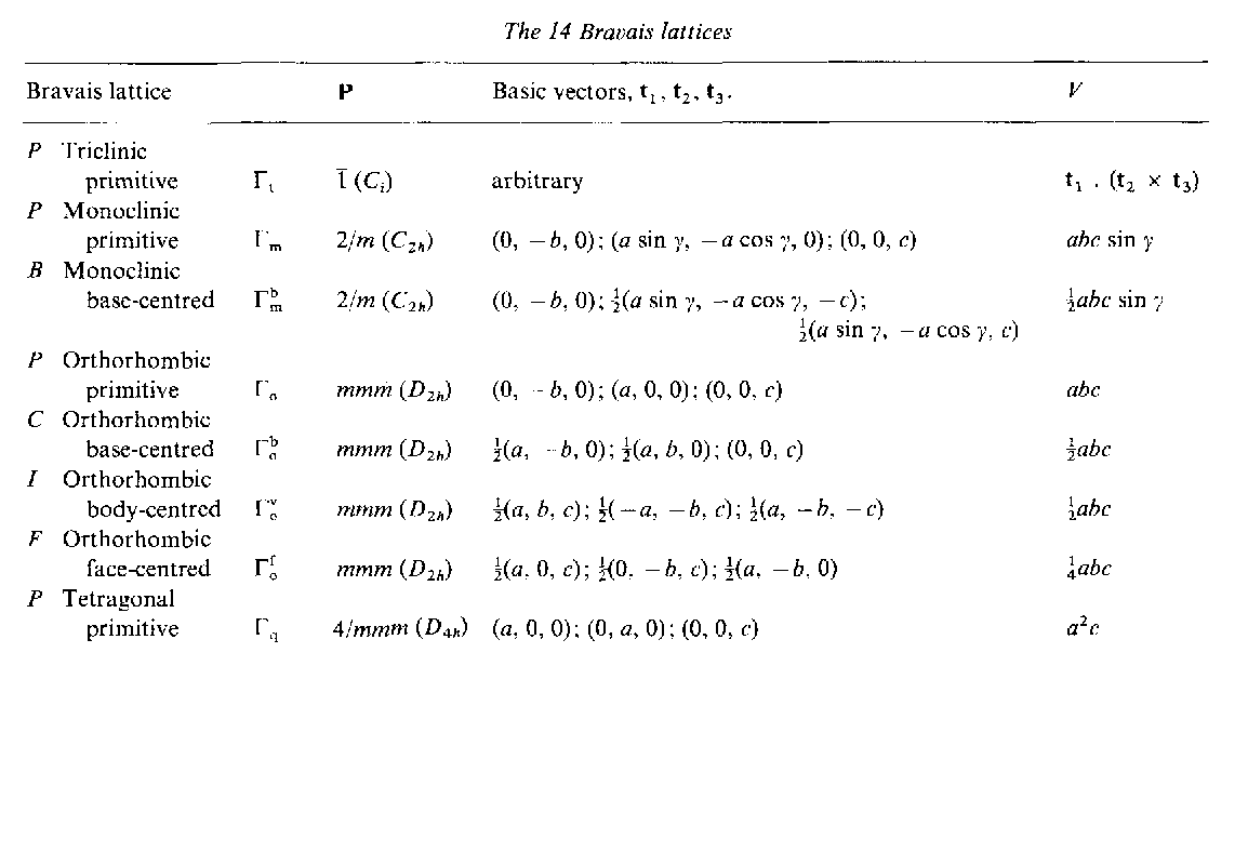
\includegraphics[width=0.92\textwidth]{c3_t31_p1.png}
\end{figure}
\begin{figure}[H]
\centering
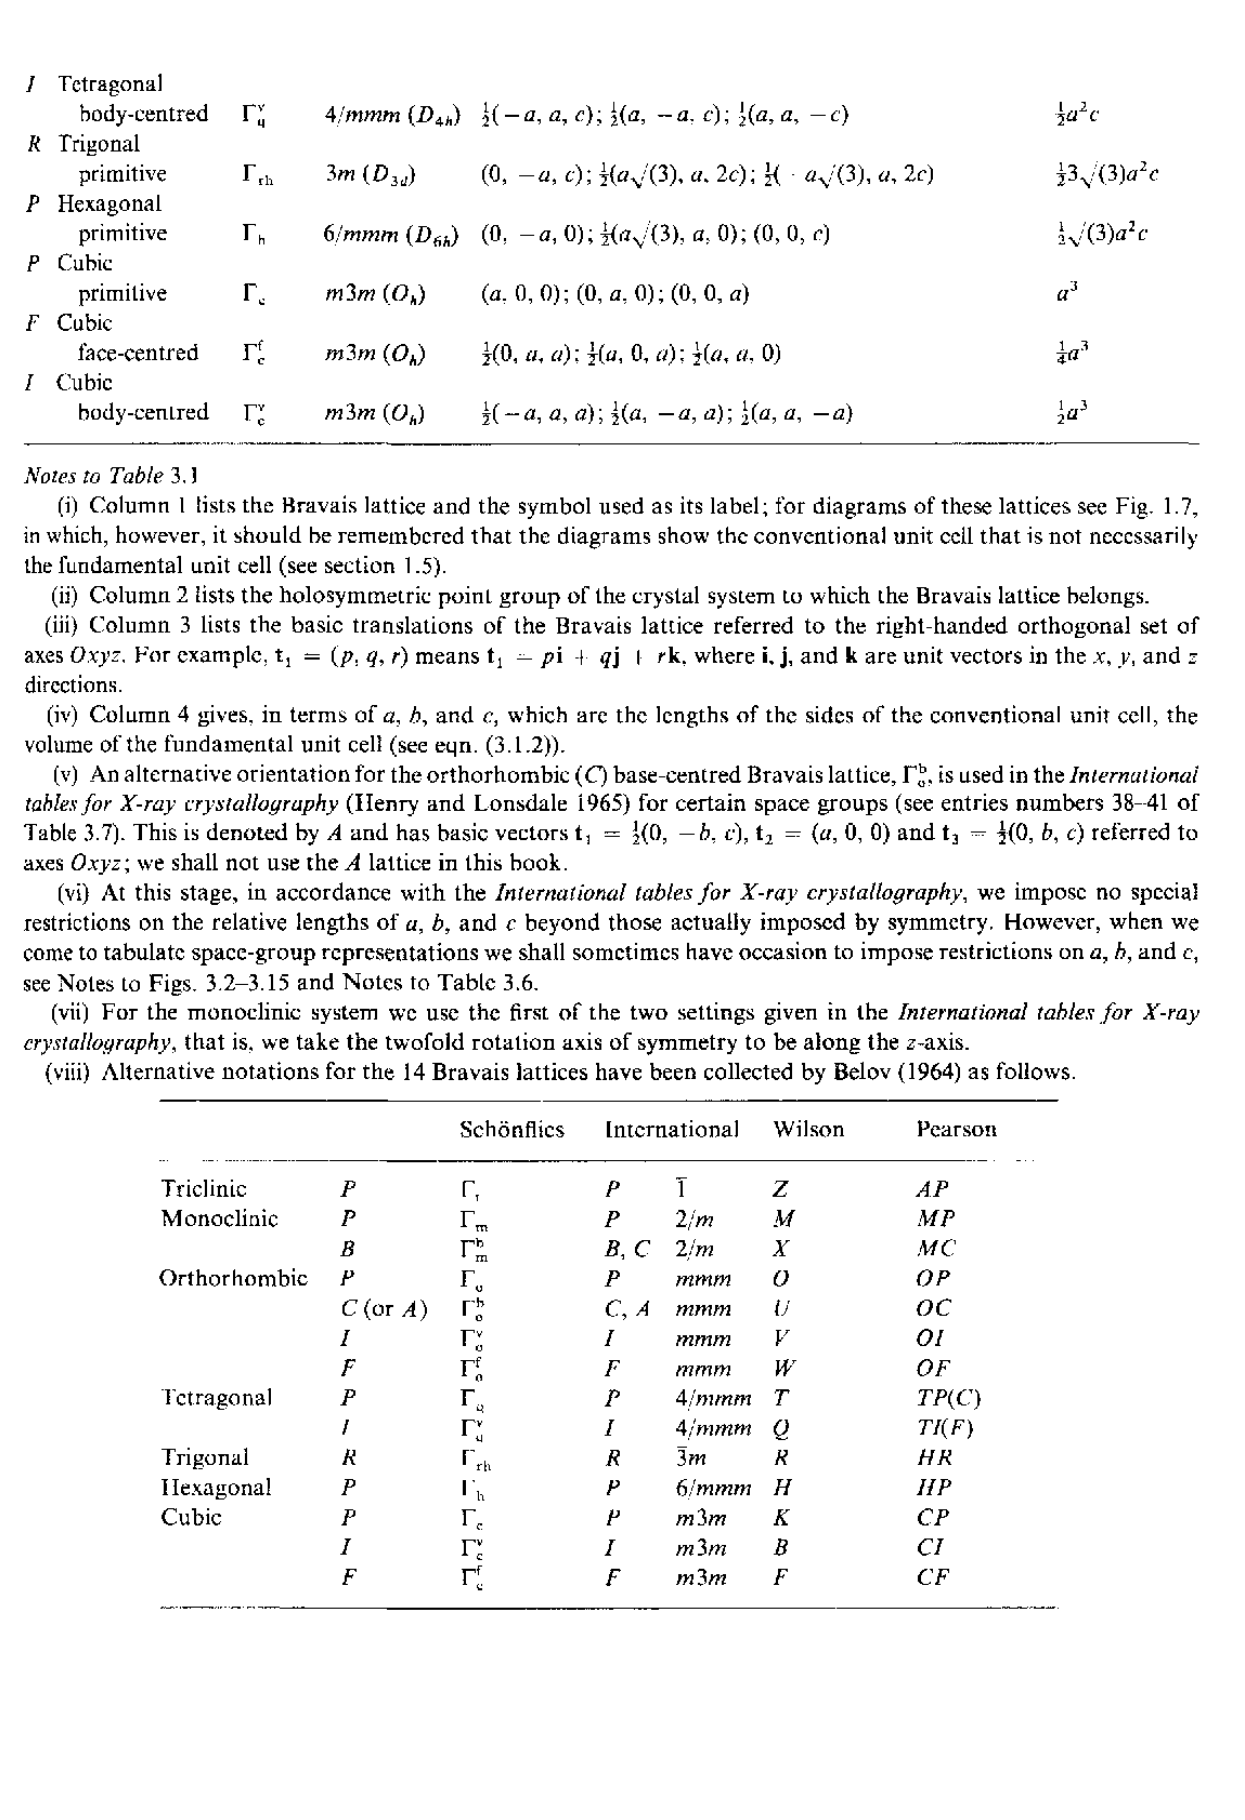
\includegraphics[width=0.92\textwidth]{c3_t31_p2.png}
\caption*{\textbf{表 3.1}\ 14 种布拉维格子：格子类型符号、Schönflies 记号 $\Gamma$、国际记号、基本平移（相对 $Oxyz$）与初基晶胞体积（原书扫描占位，含注 (i)--(viii)，见正文）。}
\end{figure}

七个晶系的对称元素见表 1.2。了解晶系的点群操作对格子平移的作用是有益的，这些作用列于表 3.2。

% 3.2 倒格子和布里渊区
\section{倒格子和布里渊区}

若布拉维格子的基本平移矢量为 $\mathbf{t}_{1}$、$\mathbf{t}_{2}$、$\mathbf{t}_{3}$，则可以定义一组倒格子（reciprocal lattice）矢量 $\mathbf{g}_{1}$、$\mathbf{g}_{2}$、$\mathbf{g}_{3}$，满足
\begin{equation*}
\mathbf{g}_{i} \cdot \mathbf{t}_{j} = 2\pi\delta_{ij} \qquad (i, j = 1, 2, 3).
\tag{3.2.1}
\end{equation*}
这样定义的倒格子当然早已为 X 射线晶体学家所广泛使用。一些作者在式中定义 $\mathbf{g}_{i}$ 时不含因子 $2\pi$，因而在后面的理论中不得不使用“$2\pi$ 乘一个倒格子矢量”这种笨拙的说法。由式 (3.2.1)，$\mathbf{g}_{1}$、$\mathbf{g}_{2}$、$\mathbf{g}_{3}$ 可显式地写为
\begin{equation*}
\left\{
\begin{array}{l}
\mathbf{g}_{1} = \dfrac{2\pi(\mathbf{t}_{2} \times \mathbf{t}_{3})}{\mathbf{t}_{1} \cdot (\mathbf{t}_{2} \times \mathbf{t}_{3})}, \\[2ex]
\mathbf{g}_{2} = \dfrac{2\pi(\mathbf{t}_{3} \times \mathbf{t}_{1})}{\mathbf{t}_{2} \cdot (\mathbf{t}_{3} \times \mathbf{t}_{1})}, \\[2ex]
\mathbf{g}_{3} = \dfrac{2\pi(\mathbf{t}_{1} \times \mathbf{t}_{2})}{\mathbf{t}_{3} \cdot (\mathbf{t}_{1} \times \mathbf{t}_{2})}.
\end{array}
\right.
\tag{3.2.2}
\end{equation*}
若 $\mathbf{t}_{1}$、$\mathbf{t}_{2}$、$\mathbf{t}_{3}$ 是某一布拉维格子的基本矢量，则 $\mathbf{g}_{1}$、$\mathbf{g}_{2}$、$\mathbf{g}_{3}$ 通常是同一布拉维格子（在倒空间中）的基本矢量。但有四种情形，$\mathbf{g}_{1}$、$\mathbf{g}_{2}$、$\mathbf{g}_{3}$ 是同一晶系中另一种布拉维格子的基本矢量。例如，考虑面心立方格子，由表 3.1 其基本矢量为
\begin{equation*}
\left\{
\begin{array}{l}
\mathbf{t}_{1} = \frac{1}{2}a(0, 1, 1), \\
\mathbf{t}_{2} = \frac{1}{2}a(1, 0, 1), \\
\mathbf{t}_{3} = \frac{1}{2}a(1, 1, 0).
\end{array}
\right.
\tag{3.2.3}
\end{equation*}
把它们代入式 (3.2.2)，得到
\begin{equation*}
\left\{
\begin{array}{l}
\mathbf{g}_{1} = \frac{2\pi}{a}(-1, 1, 1), \\
\mathbf{g}_{2} = \frac{2\pi}{a}(1, -1, 1), \\
\mathbf{g}_{3} = \frac{2\pi}{a}(1, 1, -1),
\end{array}
\right.
\tag{3.2.4}
\end{equation*}
对照表 3.1 即可看出，这些矢量定义的是一个体心立方格子。因此，立方面心格子的倒格子是立方体心格子，反之亦然；正交面心格子的倒格子同样是正交体心格子，反之亦然。四方体心格子的倒格子是它自身，因为四方面心格子同时也是轴比不同的四方体心格子。与正空间中的布拉维格子一样，我们可以把倒格子任一点的位矢 $\mathbf{g}$ 用 $\mathbf{g}_{1}$、$\mathbf{g}_{2}$、$\mathbf{g}_{3}$ 表示；仿照式 (1.5.1)，
\begin{equation*}
\mathbf{g} = n_{1}\mathbf{g}_{1} + n_{2}\mathbf{g}_{2} + n_{3}\mathbf{g}_{3}
\tag{3.2.5}
\end{equation*}
其中 $n_{1}$、$n_{2}$、$n_{3}$ 为整数。

正空间坐标我们用 $x$、$y$、$z$，倒空间坐标用 $k_{x}$、$k_{y}$、$k_{z}$，因为倒空间中的一般矢量习惯上记作 $\mathbf{k}$。应当注意，如果把倒格子叠加在正格子上作图，那么 $\mathbf{g}_{1}$ 垂直于 $\mathbf{t}_{2}$ 和 $\mathbf{t}_{3}$，并不一定沿 $\mathbf{t}_{1}$ 的方向。在空间群的表示理论中究竟为什么要引入倒空间，到 3.4 节讨论平移群的表示理论时就会明白了。

表 3.3 列出 14 种布拉维格子的倒格子矢量。倒格子基矢 $\mathbf{g}_{1}$、$\mathbf{g}_{2}$、$\mathbf{g}_{3}$ 在所属晶系点群操作 $R$ 下的变换，既可以从倒空间中的图看出，也可以解析地计算：对式 (3.2.2) 两边施加 $R$ 即可，结果列于表 3.4。任一倒格子矢量 $\mathbf{g}$ 在 $R$ 下的变换，则可对式 (3.2.5) 两边施加 $R$ 并利用表 3.4 求出。

\begin{figure}[H]
\centering
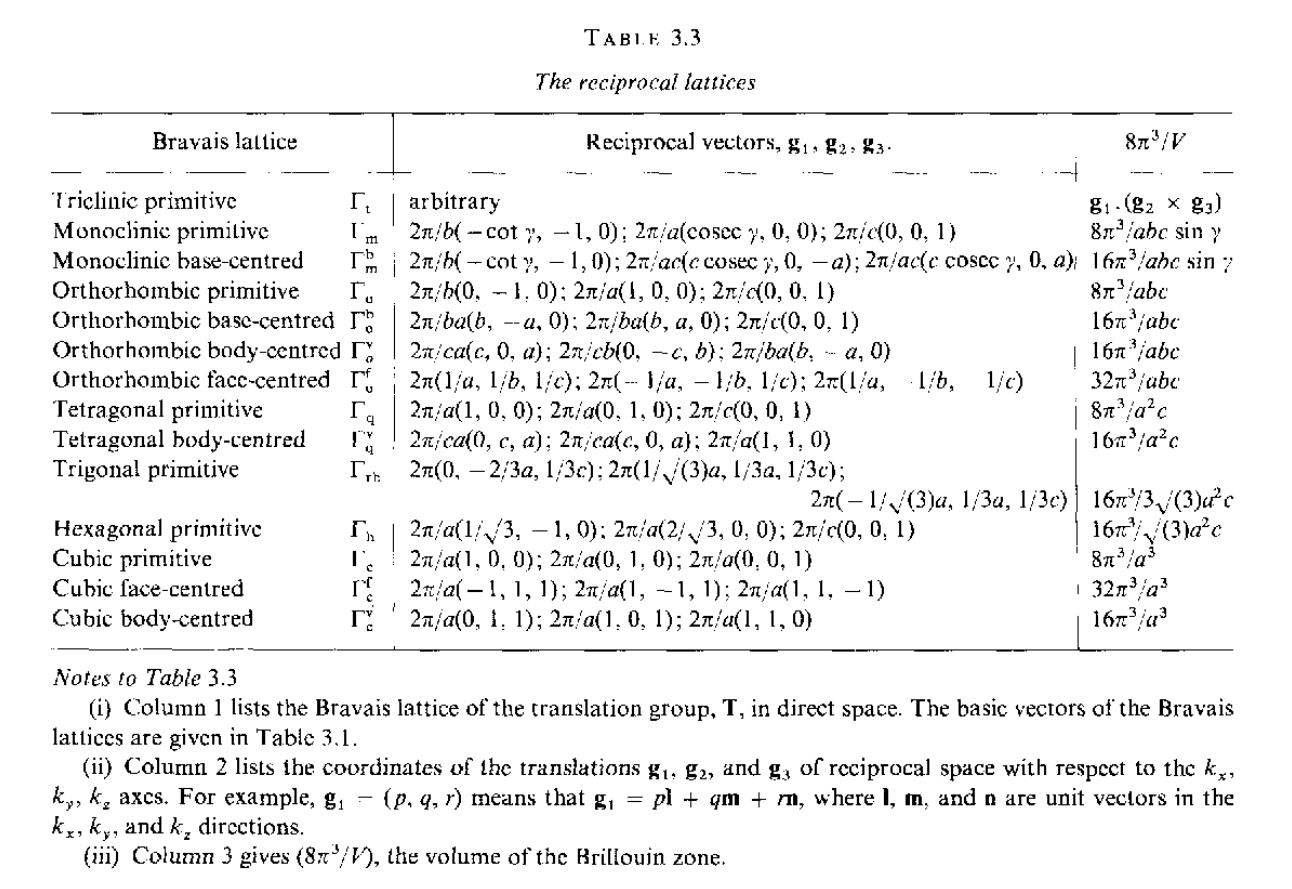
\includegraphics[width=0.92\textwidth]{c3_t33.png}
\caption*{\textbf{表 3.3}\ 倒格子（原书扫描占位）。左起各列：布拉维格子、$\Gamma$ 记号、倒格子矢量 $\mathbf{g}_{1}, \mathbf{g}_{2}, \mathbf{g}_{3}$、$8\pi^{3}/V$。注：}
\end{figure}
\noindent（i）第 1 列列出正空间平移群 $\mathbf{T}$ 的布拉维格子。各布拉维格子的基本矢量见表 3.1。

\noindent（ii）第 2 列列出倒空间平移 $\mathbf{g}_{1}$、$\mathbf{g}_{2}$、$\mathbf{g}_{3}$ 相对于 $k_{x}$、$k_{y}$、$k_{z}$ 轴的坐标。例如 $\mathbf{g}_{1} = (p, q, r)$ 表示 $\mathbf{g}_{1} = p\mathbf{l} + q\mathbf{m} + r\mathbf{n}$，其中 $\mathbf{l}$、$\mathbf{m}$、$\mathbf{n}$ 是 $k_{x}$、$k_{y}$、$k_{z}$ 方向的单位矢量。

\noindent（iii）第 3 列给出 $(8\pi^{3}/V)$，即布里渊区的体积。

\begin{figure}[H]
\centering
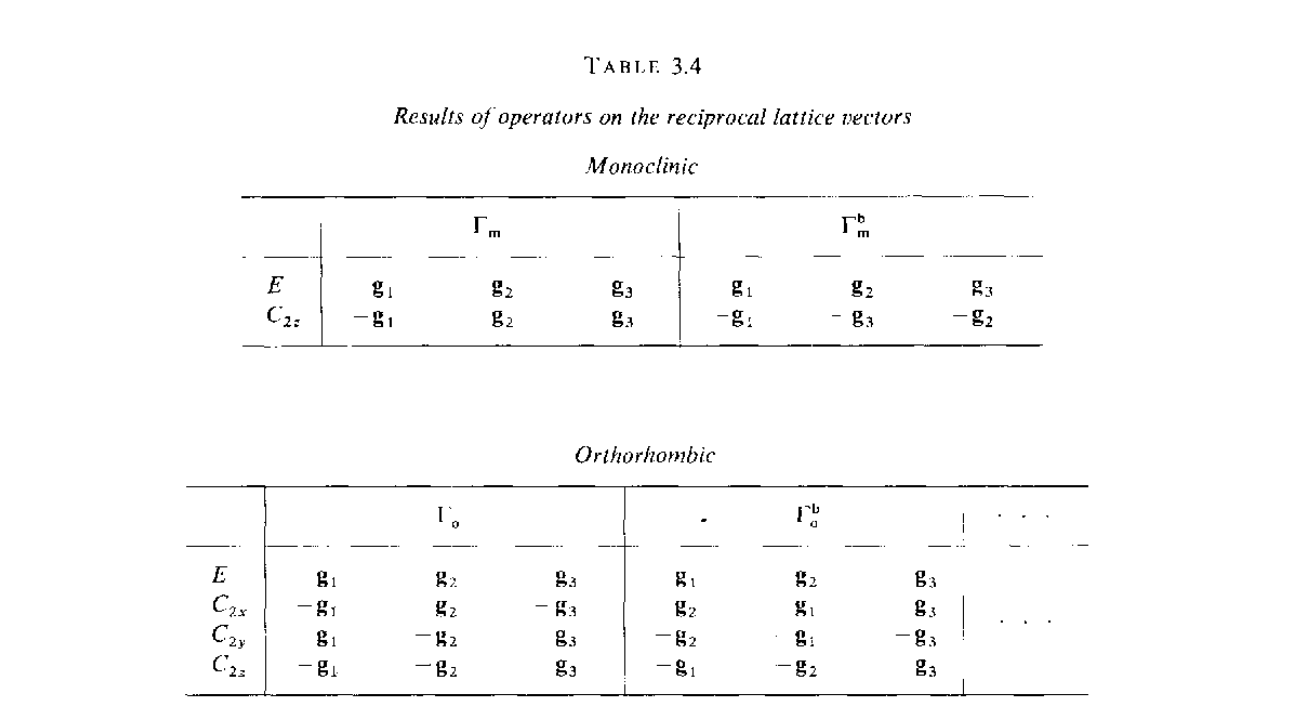
\includegraphics[width=0.78\textwidth]{c3_t34_p1.png}
\caption*{\textbf{表 3.4}\ 算符作用在倒格子矢量上的结果（第一部分：单斜、正交；原书扫描占位）。}
\end{figure}
\begin{figure}[H]
\centering
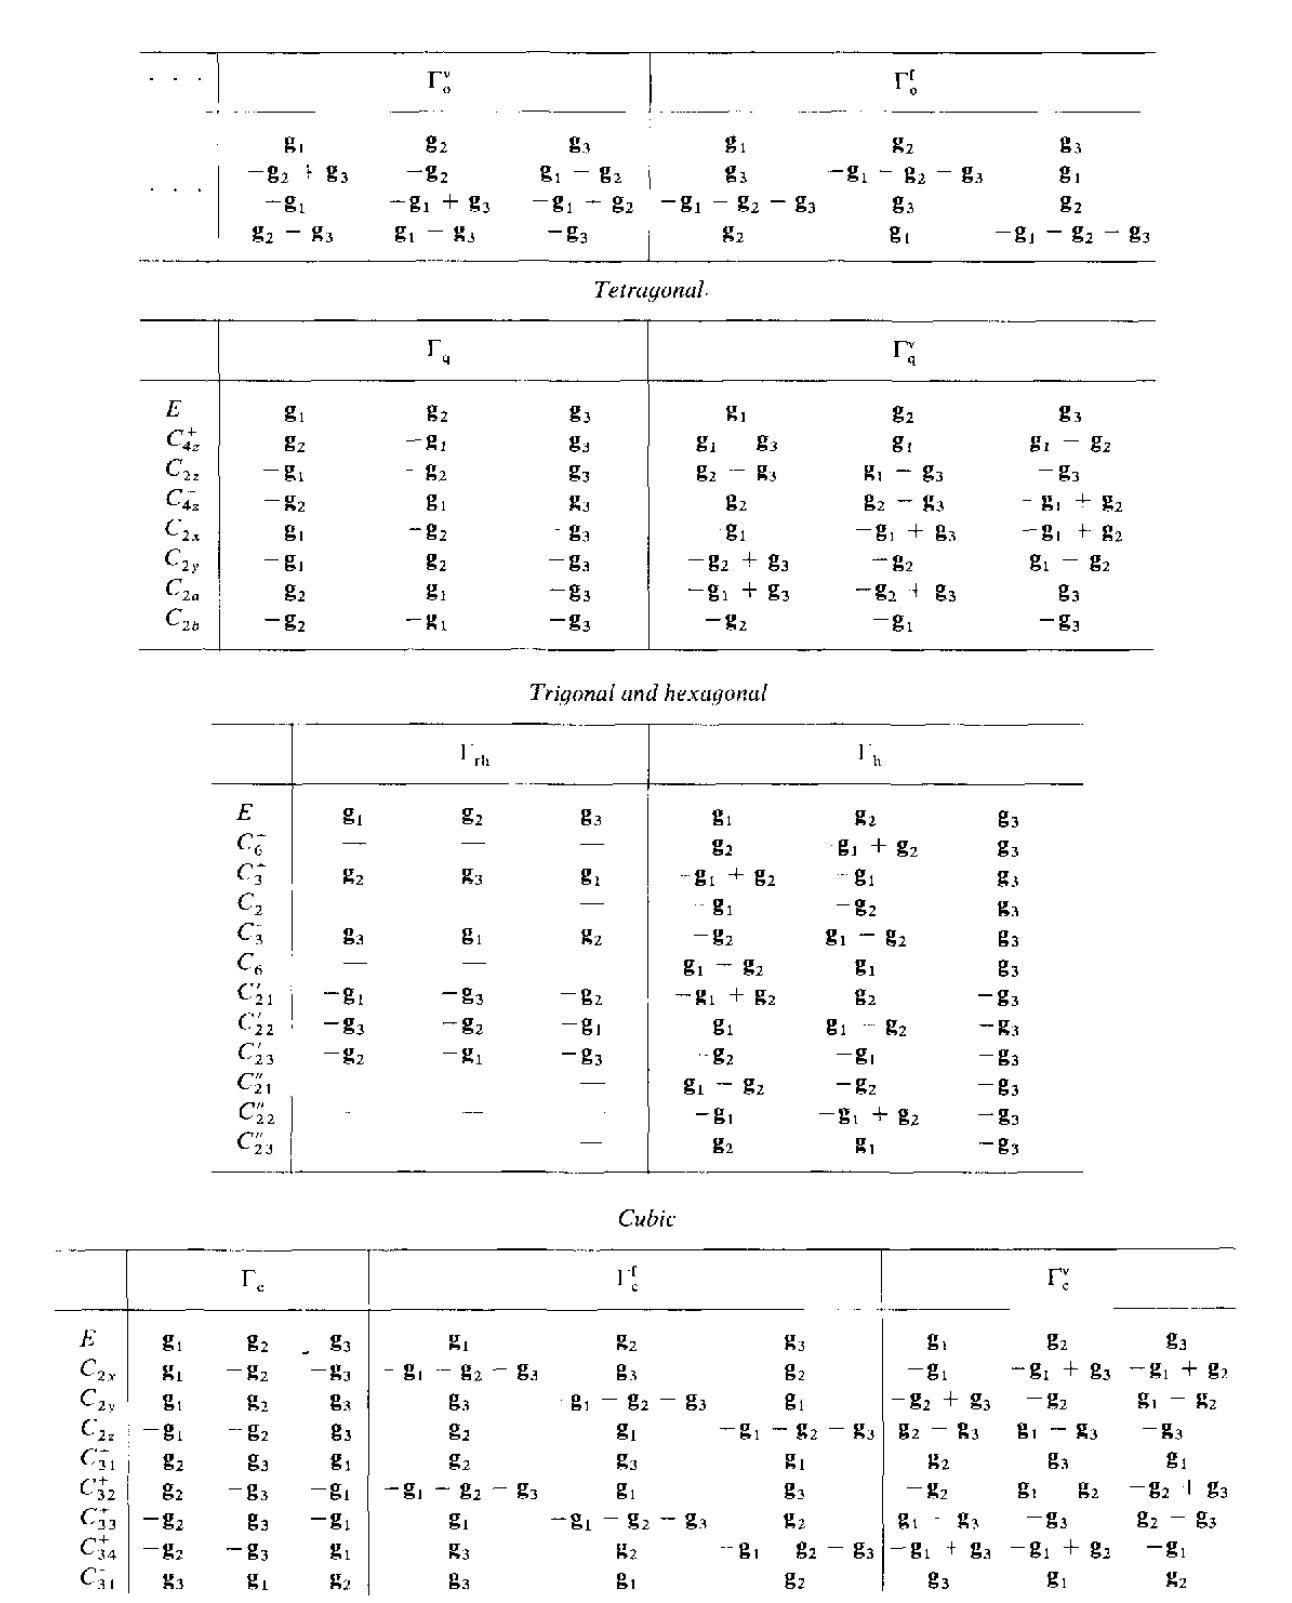
\includegraphics[width=0.86\textwidth]{c3_t34_p2.png}
\caption*{\textbf{表 3.4}（第二部分：正交续、四方、三角与六角、立方；原书扫描占位）。}
\end{figure}
\begin{figure}[H]
\centering
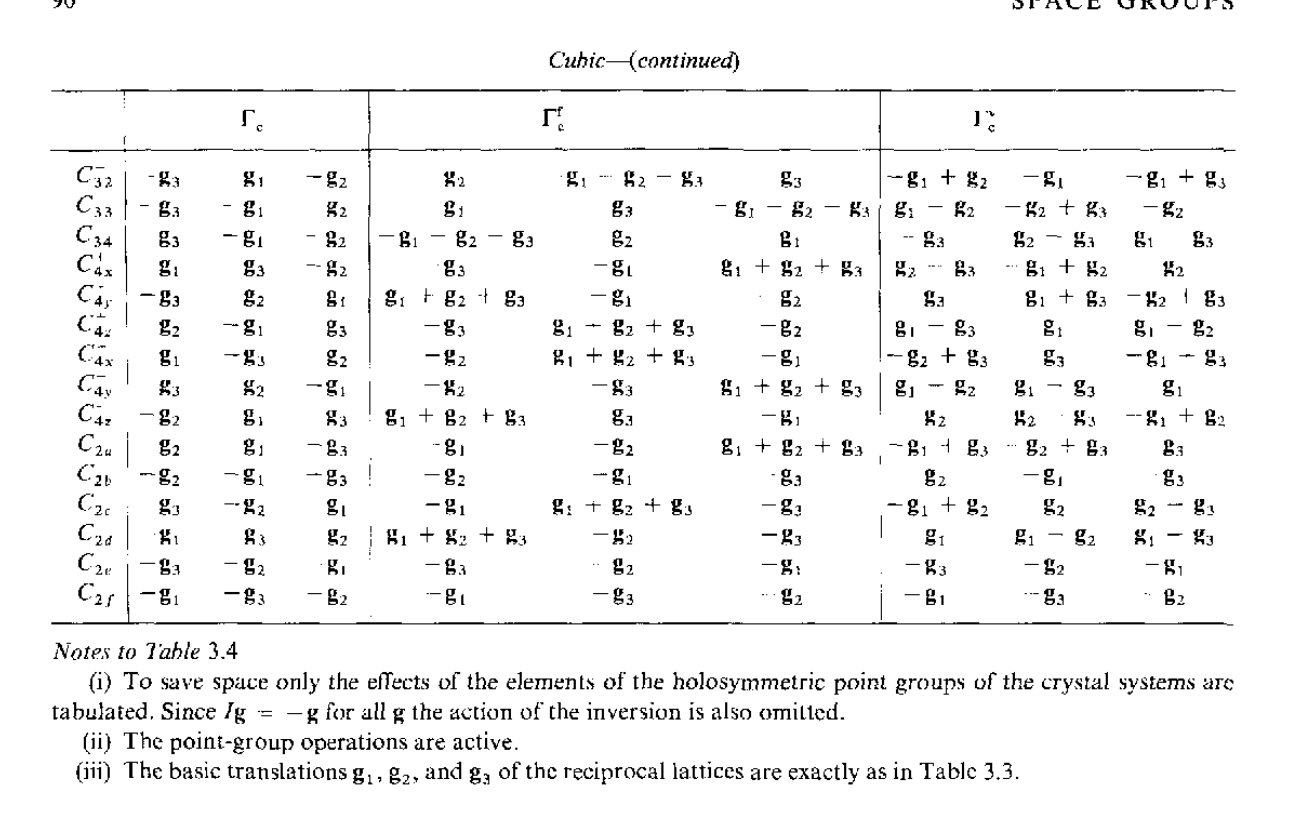
\includegraphics[width=0.88\textwidth]{c3_t34_p3.png}
\caption*{\textbf{表 3.4}（第三部分：立方续；原书扫描占位）。注：}
\end{figure}
\noindent（i）为节省篇幅，表中只列出各晶系全对称点群（holosymmetric point group）诸元素的作用。由于 $I\mathbf{g} = -\mathbf{g}$ 对一切 $\mathbf{g}$ 成立，反演的作用也一并略去。

\noindent（ii）点群操作是主动的（active）。

\noindent（iii）倒格子的基本平移 $\mathbf{g}_{1}$、$\mathbf{g}_{2}$、$\mathbf{g}_{3}$ 与表 3.3 中的完全一致。

接下来我们讨论布里渊区（Brillouin 1930\textit{a}--\textit{c}, 1931, 1953）。\textit{第一布里渊区}（first Brillouin zone）本质上是晶体倒格子的一个晶胞；这是布里渊区要发挥任何有用作用的必要条件。惯常选取的特定晶胞是倒格子的 Wigner--Seitz 晶胞（见 1.5 节）（Jones 1960, Slater 1965\textit{b}）。这时布里渊区定义如下：

\noindent\textbf{定义 3.2.1}\quad 以倒格点之一为原点的全部 $\mathbf{k}$ 矢量的集合，若具有性质：从其中任一矢量出发，加上倒格子的平移矢量，不能到达更短长度的矢量，则这个集合构成所谓\textit{第一布里渊区}。

实际上，对三斜和单斜空间群我们将不使用这个定义（见下面的定义 3.2.2）。

按这个定义构造第一布里渊区时，我们选定某个倒格点为原点，作出由它连向其余倒格点的矢量 $\mathbf{g}$。若画出这些倒格子矢量 $\mathbf{g}$ 的垂直平分面，那么第一布里渊区就是围绕原点、由这些平面围成的最小体积。$\mathbf{g}$ 的垂直平分面的方程为
\begin{equation*}
\mathbf{k} \cdot \mathbf{g} = \tfrac{1}{2}|\mathbf{g}|^{2}.
\tag{3.2.6}
\end{equation*}
于是第一布里渊区的每一个面都由一个倒格子矢量 $\mathbf{g}$ 表征，并且当然就是 $\mathbf{g}$ 的垂直平分面。之所以在倒空间选取 Wigner--Seitz 晶胞而不是别的晶胞，是因为这个晶胞展示出倒格子的点群对称性（例如见 Delaunay (1932)）。然而，对属于低对称晶系的晶体，用式 (3.2.6) 作图构造布里渊区极其繁琐。

另一种值得在此一并考虑的晶胞是初基晶胞（见 1.5 节），即以 $\mathbf{k} = \mathbf{0}$ 为中心、棱与倒格子基本矢量 $\mathbf{g}_{1}$、$\mathbf{g}_{2}$、$\mathbf{g}_{3}$ 平行且等长的平行六面体。第一布里渊区的体积便由
\begin{equation*}
\mathbf{g}_{1} \cdot (\mathbf{g}_{2} \times \mathbf{g}_{3}) = \frac{8\pi^{3}}{V}
\tag{3.2.7}
\end{equation*}
给出，其中 $V$ 是相应正格子初基晶胞的体积；每种倒格子的 $\mathbf{g}_{1} \cdot (\mathbf{g}_{2} \times \mathbf{g}_{3})$ 值见表 3.3。对某些倒格子（正交 $P$、四方 $P$ 和立方 $P$ 空间群的倒格子），用倒空间初基晶胞定义的布里渊区与用 Wigner--Seitz 晶胞定义的惯用布里渊区完全相同。对另一些倒格子（正交 $I$、四方 $I$、六角 $P$、立方 $F$ 和立方 $I$ 空间群的倒格子），初基晶胞不能在与正空间格子相同的取向上展示布拉维格子的点群对称性，此时初基晶胞便不能用来定义布里渊区，见表 3.5 第 2 列。这八种布拉维格子几乎涵盖了实际研究过布里渊区的全部晶体，因此人们通常把选取倒空间的 Wigner--Seitz 晶胞当作第一布里渊区定义的一个必要部分，这并不奇怪。然而，对其余六种布拉维格子（三斜 $P$、单斜 $P$、单斜 $B$、正交 $C$、正交 $F$ 和三方 $R$ 空间群的），可以直接看出倒格子的初基晶胞也以正确的取向具有晶体布拉维格子的点群对称性。不过，只要可能，最好让布里渊区的界面平行于晶体中的对称面。这意味着对正交 $C$ 与 $F$ 空间群，在定义布里渊区时宜保留 Wigner--Seitz 胞，见图 3.6 与图 3.8。至于三方 $R$ 格子，似乎也没有什么特别有力的理由要用倒空间的初基晶胞去取代惯用的布里渊区定义。但对剩下的三种格子（三斜 $P$、单斜 $P$ 和单斜 $B$ 空间群的），如前所述，无论要画出布里渊区的形状，还是画出之后要在头脑中想象它，式 (3.2.6) 在实际应用中都十分困难，其形状细节在很大程度上依赖于所论晶体晶胞参数的具体取值。对单斜晶体，一些作者（Koster 1957, Sushkevich 1966）对每种布拉维格子各画出一个特定例子，Luehrmann (1968) 对单斜 $B$ 格子给出了两个例子，而 Kovalev (1965) 的详表则完全没有布里渊区图。因此，对单斜或三斜晶体采用初基晶胞定义布里渊区有一个优点：其总体形状（即棱数和面数）不依赖于晶体晶胞的轴比和轴间角。

\begin{table}[H]
\centering
\caption*{\textbf{表 3.5}\ 第 2 列标出：由倒空间初基晶胞定义的布里渊区是否以正确取向具有晶体的点群对称性；第 3 列标出：满足前一条件、且倒空间的 Wigner--Seitz 胞与初基胞给出相同布里渊区形状的那些布拉维格子。}
\begin{tabular}{@{}lcccclccc@{}}
\toprule
布拉维格子 & 2 & 3 & \phantom{xxxx} & 布拉维格子 & 2 & 3 \\
\midrule
三斜 $P$   & $\checkmark$ & $\times$ & & 四方 $P$ & $\checkmark$ & $\checkmark$ \\
单斜 $P$   & $\checkmark$ & $\times$ & & 四方 $I$ & $\times$ & --- \\
单斜 $B$   & $\checkmark$ & $\times$ & & 三方 $R$ & $\checkmark$ & $\times$ \\
正交 $P$   & $\checkmark$ & $\checkmark$ & & 六角 $P$ & $\times$ & --- \\
正交 $C$   & $\checkmark$ & $\times$ & & 立方 $P$ & $\checkmark$ & $\checkmark$ \\
正交 $I$   & $\times$ & --- & & 立方 $F$ & $\times$ & --- \\
正交 $F$   & $\checkmark$ & $\times$ & & 立方 $I$ & $\times$ & --- \\
\bottomrule
\end{tabular}
\end{table}

因此我们建议：大多数晶体的布里渊区仍用倒空间的 Wigner--Seitz 胞来定义，但对单斜和三斜空间群，应当改用倒空间的初基晶胞（Bradley and Cracknell 1970）。在构造图 3.2--3.4 时我们遵循了这一做法。

\noindent\textbf{定义 3.2.2}\quad 对单斜或三斜晶体，第一布里渊区取为倒格子的初基晶胞，即以 $\mathbf{k} = \mathbf{0}$ 为中心、棱与倒格子基本矢量 $\mathbf{g}_{1}$、$\mathbf{g}_{2}$、$\mathbf{g}_{3}$ 平行且等长的平行六面体。

最后还应指出一点。有人认为式 (3.2.6) 与电子、声子或磁振子的能量 $E(\mathbf{k})$ 随 $\mathbf{k}$ 变化曲线中出现不连续有特殊关联。其实并非如此，因为无论在扩展区图式还是重复区图式中，$E(\mathbf{k})$ 在倒空间处处都是 $\mathbf{k}$ 的准连续函数（Koopmans 定理）。划定区界时出现的不连续，不过是不同的 $E(\mathbf{k})$ 曲线在此分开。当然，有时可以细心地选取区界，使得 $E(\mathbf{k})$ 在区界处呈现特殊的简并；然而这一性质来源于“布里渊区应当展示布拉维格子的正确点群对称性”这一要求——我们并没有放弃这个要求——而不是使用 Wigner--Seitz 胞和式 (3.2.6) 的结果。

用式 (3.2.6) 构造第一布里渊区时，倒格子矢量 $\mathbf{g}$ 是由原点连向它的第一近邻、可能还有第二或更远近邻的矢量。还可以利用式 (3.2.6) 的更多平面，在第一布里渊区之外围出一个满足下列三个条件的体积，从而定义第二布里渊区：(i) 第二布里渊区的体积等于第一布里渊区的体积；(ii) 对第一布里渊区中的每个 $\mathbf{k}$ 矢量 $\mathbf{k}_{1}$，在第二布里渊区中恰有一个 $\mathbf{k}$ 矢量 $\mathbf{k}_{2}$，使得
\begin{equation*}
\mathbf{k}_{2} - \mathbf{k}_{1} = \mathbf{g},
\tag{3.2.8}
\end{equation*}
其中 $\mathbf{g}$ 是一个倒格子矢量，但对所有 $\mathbf{k}_{1}$ 不必相同。于是，第二布里渊区中的每一点都在某种意义上（3.3 节将更严格地定义）等价于第一布里渊区中的某一点；(iii) 第二布里渊区中的 $\mathbf{k}$ 矢量必须取满足条件 (i) 与 (ii) 的最短者。类似地可以定义第三、第四以及更高阶的布里渊区。

在给任一给定晶体定义布里渊区时，务必小心使用描述晶体\textit{全部}平移对称性的布拉维格子，而不要用晶胞更大的其他格子（Barron and Fischer 1959）。一旦完整认定了布拉维格子，倒格子与布里渊区的结构便唯一确定；它们与晶胞内部原子的具体排布完全无关。如上定义的布里渊区具有如下性质：

\noindent(i) 晶体的布拉维格子每个初基晶胞在区中对应一个态（对电子，泡利不相容原理允许自旋为 $+\frac{1}{2}$ 和 $-\frac{1}{2}$ 的两个电子占据每个这样的态；对声子或磁振子，当然不存在这样的不相容原理）（见式 (3.4.5)）。

\noindent(ii) 晶体中粒子或准粒子的能量在每个区内部处处连续。

\noindent(iii) 更高阶区的各分区可以通过适当的倒格子矢量平移而搬入第一区，这样每个区的态便在第一区上构成一条连续能带；这称为\textit{约化区图式}（reduced zone scheme）。

\noindent(iv) 具有第一布里渊区形状的胞可以相互拼合，完全填满倒空间，即相邻胞之间不留空隙。这称为\textit{重复区图式}（repeated zone scheme），常常有用。

在倒空间中定义区的另一种方法（Jones 1934\textit{a}）主张：只有那些对应的 Bragg 反射具有非零结构因子（structure factor）的平面才是真正的区界。这些 \textit{Jones 区}（Jones zones）在许多标准教科书中已有讨论（例如 Jones (1960), Kittel (1956), Mott and Jones (1936), Wilson (1953)），但如今似乎已很少使用。

\begin{figure}[H]
\centering
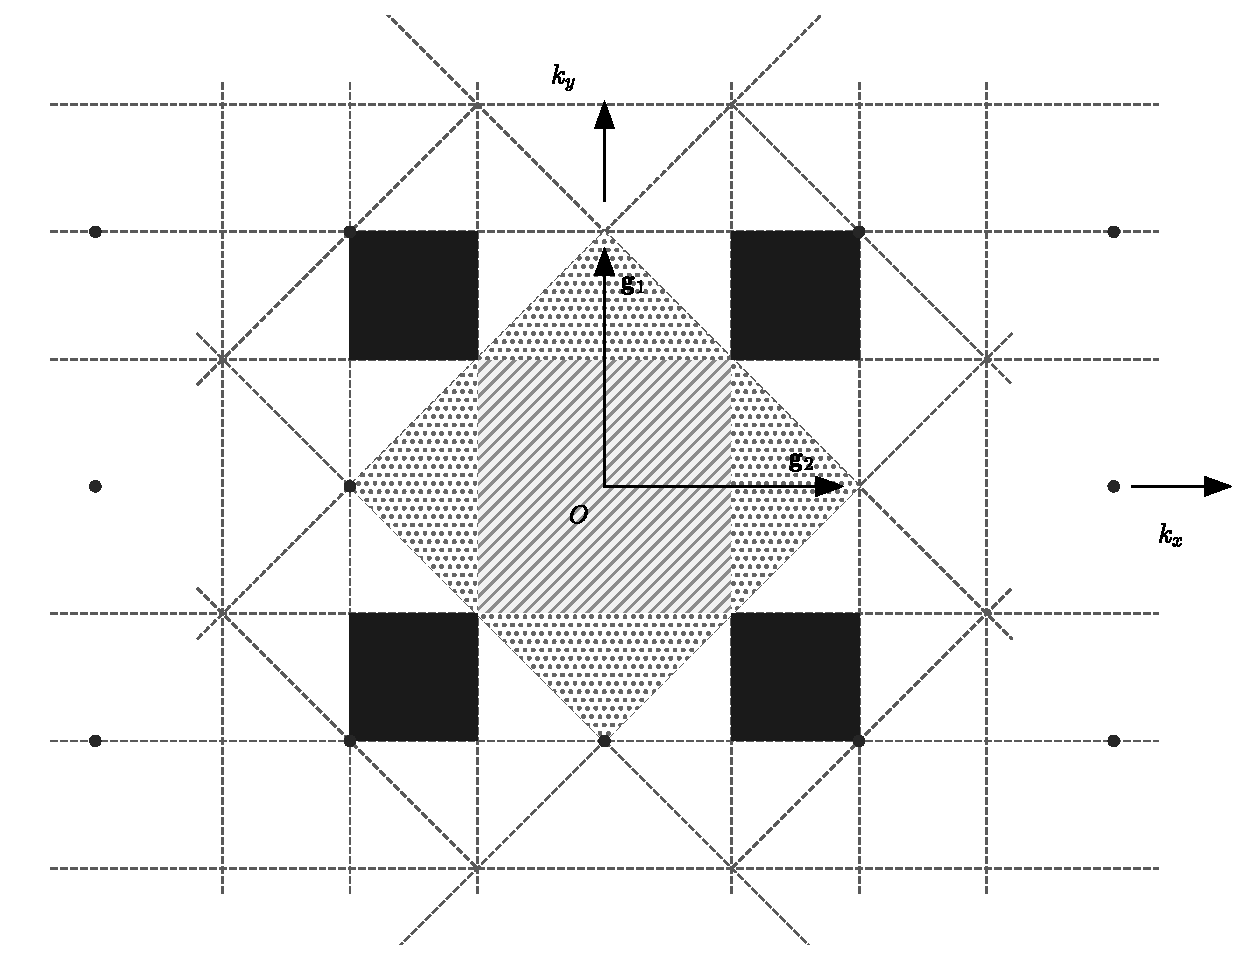
\includegraphics[width=0.92\textwidth]{fig3_1.pdf}
\caption{二维正方布拉维格子 $p$ 的前三个布里渊区（依原书重绘）。}
\end{figure}

我们用一个二维的例子来说明第一、第二及更高阶布里渊区的概念。二维正方布拉维格子 $p$ 的基本矢量可取为
\begin{equation*}
\left\{
\begin{array}{l}
\mathbf{t}_{1} = a\mathbf{i} \\
\mathbf{t}_{2} = a\mathbf{j}
\end{array}
\right.
\tag{3.2.9}
\end{equation*}
其中 $\mathbf{i}$、$\mathbf{j}$ 是 $x$、$y$ 方向的单位矢量。满足式 (3.2.1) 的倒格子矢量 $\mathbf{g}_{1}$、$\mathbf{g}_{2}$ 于是为
\begin{equation*}
\left\{
\begin{array}{l}
\mathbf{g}_{1} = \frac{2\pi}{a}\mathbf{j} \\
\mathbf{g}_{2} = \frac{2\pi}{a}\mathbf{i}.
\end{array}
\right.
\tag{3.2.10}
\end{equation*}
第一布里渊区是 $k_{x} = \pm\frac{1}{2}|\mathbf{g}_{2}| = \pm\pi/a$ 与 $k_{y} = \pm\frac{1}{2}|\mathbf{g}_{1}| = \pm\pi/a$ 之间的区域，也就是说，代入式 (3.2.6) 的矢量 $\mathbf{g}$ 是 $+\mathbf{g}_{1}$、$-\mathbf{g}_{1}$、$+\mathbf{g}_{2}$ 和 $-\mathbf{g}_{2}$。于是第一布里渊区就是图 3.1 中画有斜线阴影的正方形。对第二布里渊区，代入式 (3.2.6) 的矢量是 $\mathbf{g}_{1}+\mathbf{g}_{2}$、$-\mathbf{g}_{1}+\mathbf{g}_{2}$、$\mathbf{g}_{1}-\mathbf{g}_{2}$ 和 $-\mathbf{g}_{1}-\mathbf{g}_{2}$，第二布里渊区因而是图 3.1 中标有点点的区域。事实上我们只使用第一布里渊区，所以从现在起省略“第一”这个定语。

按照 Bouckaert, Smoluchowski, and Wigner (1936) 的说法，这些区的存在几乎同时被多位作者注意到（Bloch 1928, Morse 1930, Peierls 1930, Strutt 1928\textit{a},\textit{b}），而 Brillouin（1930\textit{a}--\textit{c}, 1931）指出了它们与 X 射线反射的联系。关于布里渊区已有一本教科书（Jones 1960）。

% 3.3 对称点和对称线的分类
\section{对称点和对称线的分类}

对某些格子，布里渊区的形状是唯一的；而对另一些格子，则有两种或更多种可能的形状，取决于基本平移的相对大小和它们之间的夹角。正空间 14 种布拉维格子的各种布里渊区示于图 3.2--3.15。

若 $(\mathbf{k}_{1} - \mathbf{k}_{2}) = a_{1}\mathbf{g}_{1} + a_{2}\mathbf{g}_{2} + a_{3}\mathbf{g}_{3}$，其中 $a_{1}$、$a_{2}$、$a_{3}$ 为整数，则称矢量 $\mathbf{k}_{1}$ 与 $\mathbf{k}_{2}$ \textit{等价}。由于其构造方式，布里渊区内部任何两点都不等价；但区面上的一个点可以与区面上一个或多个其他点等价。例如，一个面的中点总与对面中点等价，因为相对的面总相差一个倒格子矢量。

给定一个布里渊区和区内一点 $\mathbf{k}$，相应晶系的全对称点群 $\mathbf{P}$ 中存在某些元素，它们把 $\mathbf{k}$ 变换到它自身或某个与它等价的 $\mathbf{k}$ 矢量。这些元素构成 $\mathbf{P}$ 的一个子群，记作 $\mathbf{P}(\mathbf{k})$，称为 $\mathbf{k}$ 的\textit{对称群}（symmetry group）。现在可以给出对称点、对称线和对称面的定义。

\noindent\textbf{定义 3.3.1}\quad 若存在 $\mathbf{k}$ 的一个邻域 $N$，使得在 $N$ 内除 $\mathbf{k}$ 以外没有任何点具有对称群 $\mathbf{P}(\mathbf{k})$，则称 $\mathbf{k}$ 是一个\textit{对称点}（point of symmetry）。

也就是说，若 $\mathbf{k}' \in N$ 且 $\mathbf{k}' \neq \mathbf{k}$，则 $\mathbf{P}(\mathbf{k}')$ 总是 $\mathbf{P}(\mathbf{k})$ 的真子群。我们可以粗略地说，点 $\mathbf{k}$ 比它周围所有的点对称性都高。

\noindent\textbf{定义 3.3.2}\quad 若在 $\mathbf{k}$ 的任一充分小邻域 $N$ 中，总有一条线（一个平面）穿过 $\mathbf{k}$，其上所有点都与 $\mathbf{k}$ 具有相同的对称群，则称 $\mathbf{k}$ 是一条\textit{对称线}（line of symmetry）（一个\textit{对称面}（plane of symmetry））。

最后，若在 $\mathbf{k}$ 的任一充分小邻域 $N$ 中所有点都具有相同的对称群，则称 $\mathbf{k}$ 为\textit{一般点}（general point）。对一般点，$\mathbf{P}(\mathbf{k})$ 仅由恒等元构成。对对称面，$\mathbf{P}(\mathbf{k})$ 由恒等元和一个镜面反射构成，只有两个元素。

\noindent\textbf{定义 3.3.3}\quad 对每个布里渊区存在一个\textit{基本域}（basic domain）$\Omega$，使得 $(\Sigma_{R} R\Omega)$ 等于整个布里渊区，其中 $R$ 取遍相关晶系全对称点群 $\mathbf{P}$ 的元素。

因此
\begin{equation*}
\Omega = \frac{8\pi^{3}}{V|\mathbf{P}|}
\tag{3.3.1}
\end{equation*}
其中 $|\mathbf{P}|$ 是 $\mathbf{P}$ 的阶。

对称点的求法是：对交于该点的各个平面使用式 (3.2.6)，算出每个面心和每个顶点的坐标，然后看在相关全对称点群 $\mathbf{P}$ 的操作下（见表 3.1），这些点是否具有邻域内其他点都不具备的额外对称操作。这里所说的对称操作是指把矢量 $\mathbf{k}$ 变换为 $\mathbf{k}$ 本身或与 $\mathbf{k}$ 相差一个倒格子矢量的矢量 $\mathbf{k}'$ 的操作。类似的手续也可用于辨认对称线。所有布拉维格子布里渊区的各种对称点和对称线都已在图 3.2--3.15 的图中标出。我们在图 3.2--3.15 中用于对称点和对称线的字母几乎都是标准的，并尽可能与前人（Bouckaert, Smoluchowski, and Wigner 1936, Herring 1942, Koster 1955, Luehrmann 1968, Meijer and Bauer 1962, Miller and Love 1967）的记号一致。

% ---- 图 3.2 -- 3.6（MinerU 提取图；题注坐标已逐条对照扫描页核对，见进度文件）----
\begin{figure}[H]
\centering
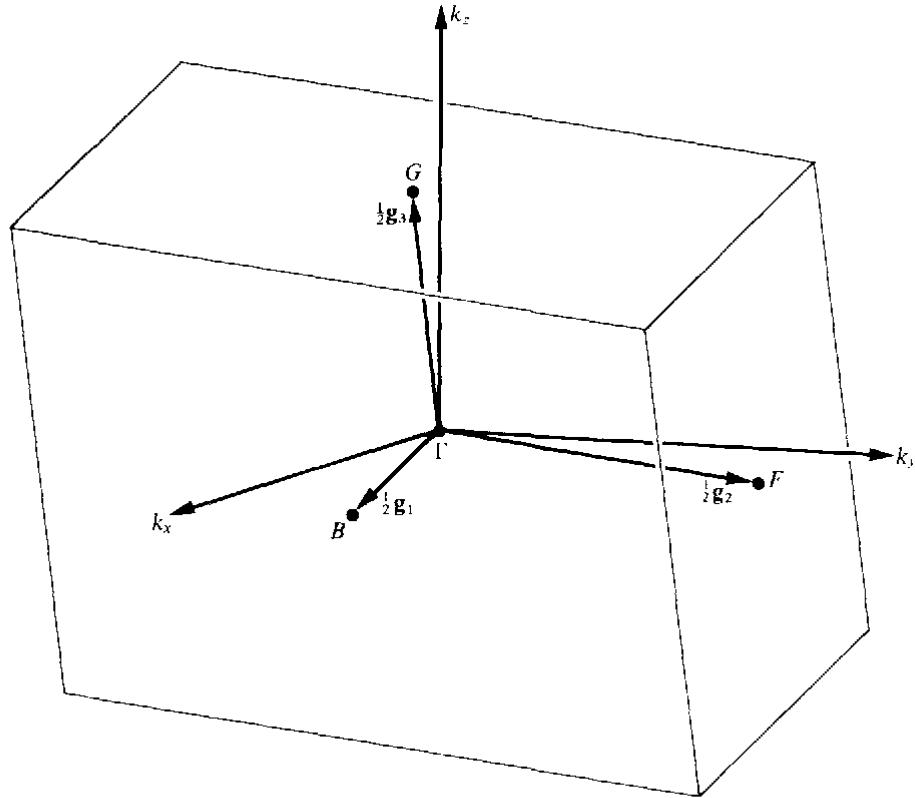
\includegraphics[width=0.60\textwidth]{fig3_2_mu.jpg}
\caption*{\textbf{图 3.2}\ $\Gamma_{t}$（三斜 $P$）的布里渊区。$\Gamma=(000)$；$B=(\frac{1}{2}00)$；$F=(0\frac{1}{2}0)$；$G=(00\frac{1}{2})$。}
\end{figure}
\begin{figure}[H]
\centering
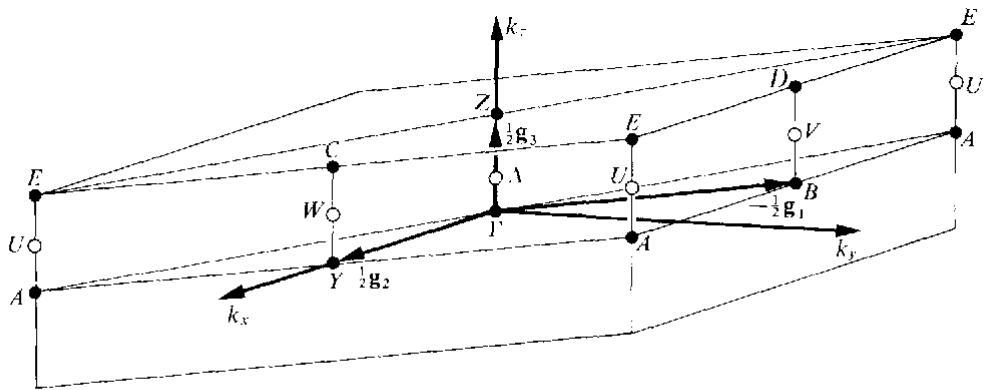
\includegraphics[width=0.64\textwidth]{fig3_3_mu.jpg}
\caption*{\textbf{图 3.3}\ $\Gamma_{m}$（单斜 $P$）的布里渊区。$\Gamma=(000)$；$B=(\bar{\frac{1}{2}}00)$；$Y=(0\frac{1}{2}0)$；$Z=(00\frac{1}{2})$；$C=(0\frac{1}{2}\frac{1}{2})$；$D=(\bar{\frac{1}{2}}0\frac{1}{2})$；$A=(\bar{\frac{1}{2}}\bar{\frac{1}{2}}0)$、$(\bar{\frac{1}{2}}\frac{1}{2}0)$ 或 $(\frac{1}{2}\bar{\frac{1}{2}}0)$；$E=(\bar{\frac{1}{2}}\bar{\frac{1}{2}}\frac{1}{2})$、$(\bar{\frac{1}{2}}\frac{1}{2}\frac{1}{2})$ 或 $(\frac{1}{2}\bar{\frac{1}{2}}\frac{1}{2})$。}
\end{figure}
\begin{figure}[H]
\centering
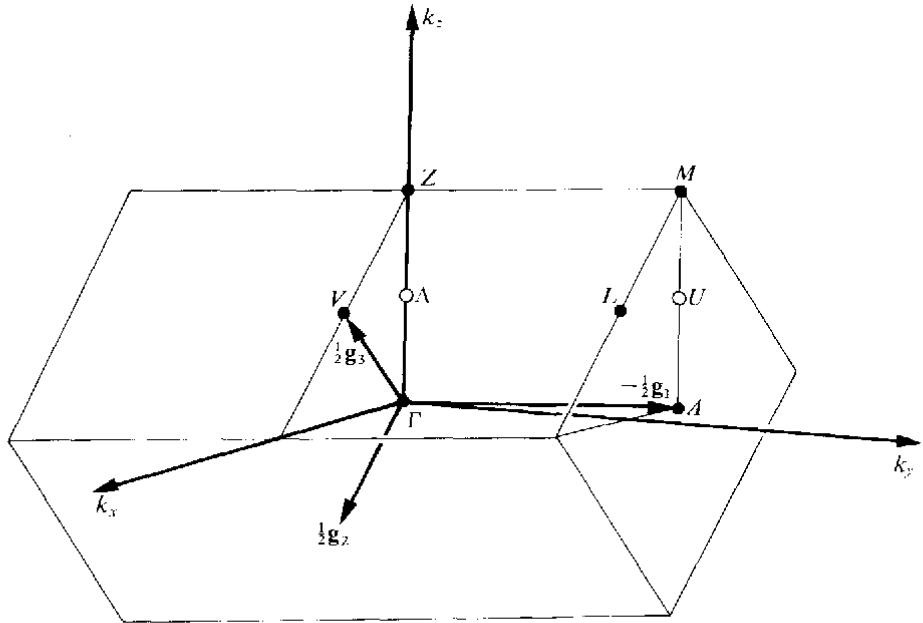
\includegraphics[width=0.64\textwidth]{fig3_4_mu.jpg}
\caption*{\textbf{图 3.4}\ $\Gamma_{m}^{b}$（单斜 $B$）的布里渊区。$\Gamma=(000)$；$A=(\frac{1}{2}00)$；$Z=(0\frac{1}{2}\frac{1}{2})$；$M=(\frac{1}{2}\frac{1}{2}\frac{1}{2})$；$L=(\frac{1}{2}0\frac{1}{2})$；$V=(00\frac{1}{2})$。}
\end{figure}
\begin{figure}[H]
\centering
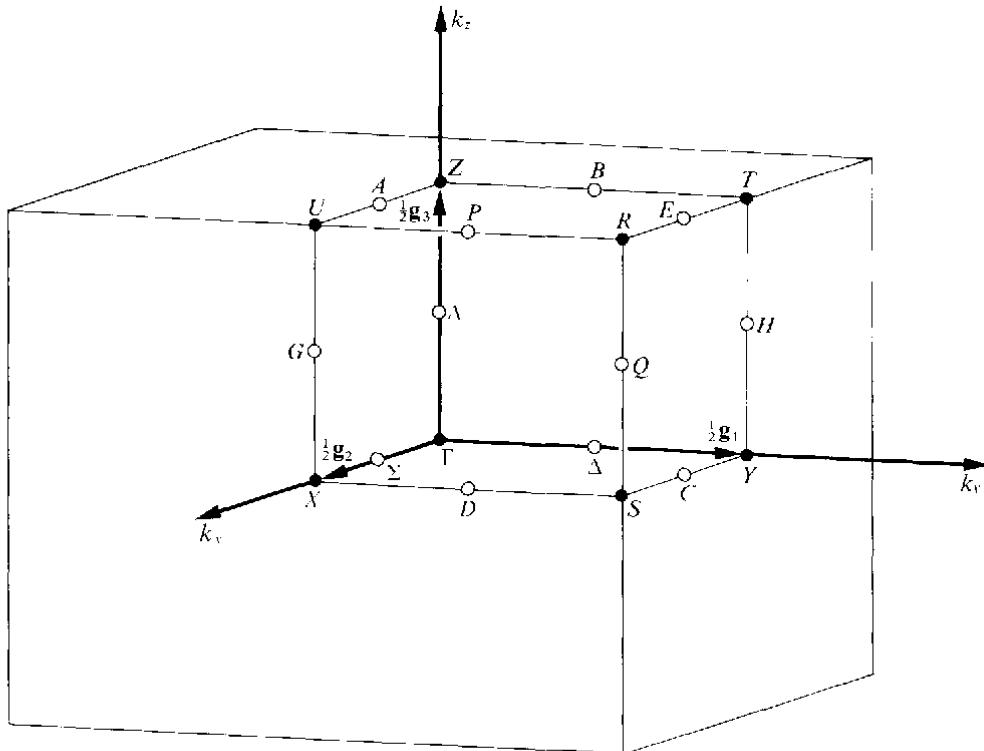
\includegraphics[width=0.64\textwidth]{fig3_5_mu.jpg}
\caption*{\textbf{图 3.5}\ $\Gamma_{o}$（正交 $P$）的布里渊区。$\Gamma=(000)$；$Y=(\frac{1}{2}00)$；$X=(0\frac{1}{2}0)$；$Z=(00\frac{1}{2})$；$U=(0\frac{1}{2}\frac{1}{2})$；$T=(\frac{1}{2}0\frac{1}{2})$；$S=(\frac{1}{2}\frac{1}{2}0)$；$R=(\frac{1}{2}\frac{1}{2}\frac{1}{2})$。}
\end{figure}
\begin{figure}[H]
\centering
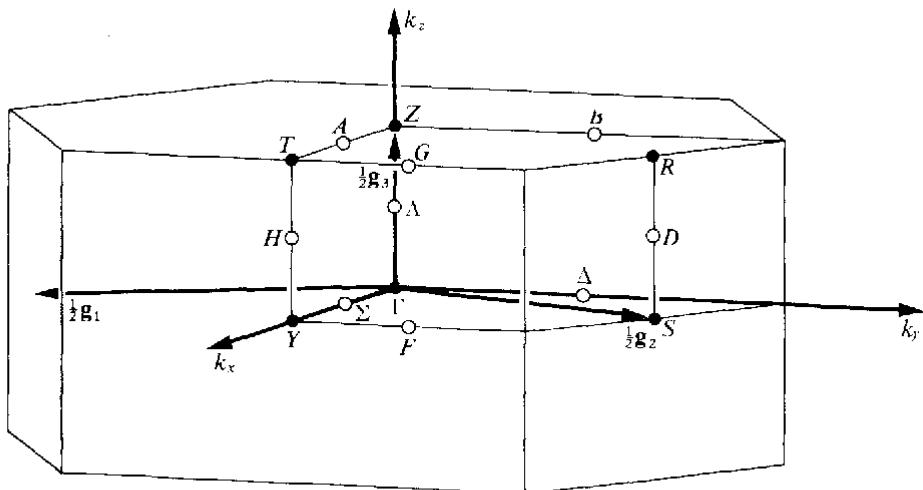
\includegraphics[width=0.58\textwidth]{fig3_6a_mu.jpg}\\[1ex]
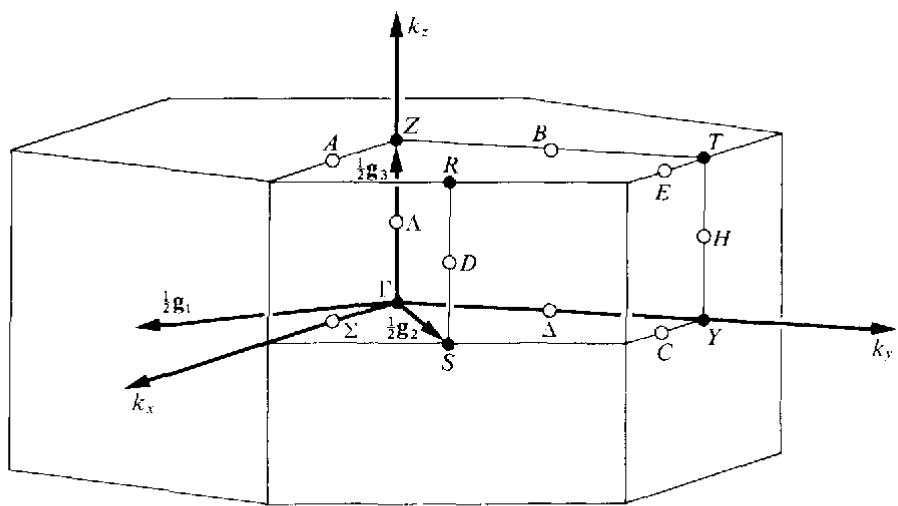
\includegraphics[width=0.58\textwidth]{fig3_6b_mu.jpg}
\caption*{\textbf{图 3.6}\ $\Gamma_{o}^{b}$（正交 $C$）的布里渊区：(a) $a>b$，$\Gamma=(000)$；$Y=(\frac{1}{2}\frac{1}{2}0)$；$Z=(00\frac{1}{2})$；$T=(\frac{1}{2}\frac{1}{2}\frac{1}{2})$；$S=(0\frac{1}{2}0)$；$R=(0\frac{1}{2}\frac{1}{2})$；(b) $b>a$，$\Gamma=(000)$；$Y=(\frac{1}{2}\frac{1}{2}0)$；$Z=(00\frac{1}{2})$；$T=(\frac{1}{2}\frac{1}{2}\frac{1}{2})$；$S=(0\frac{1}{2}0)$；$R=(0\frac{1}{2}\frac{1}{2})$。}
\end{figure}

在继续讲下面的图之前，先说明一下我们的做法。对三斜布拉维格子（图 3.2）和两种单斜布拉维格子（图 3.3 与图 3.4），我们按照定义 3.2.2 用倒空间的初基晶胞来定义布里渊区（见图注 (ii)）。其余格子的布里渊区用倒空间的 Wigner--Seitz 晶胞定义。

\begin{figure}[H]
\centering
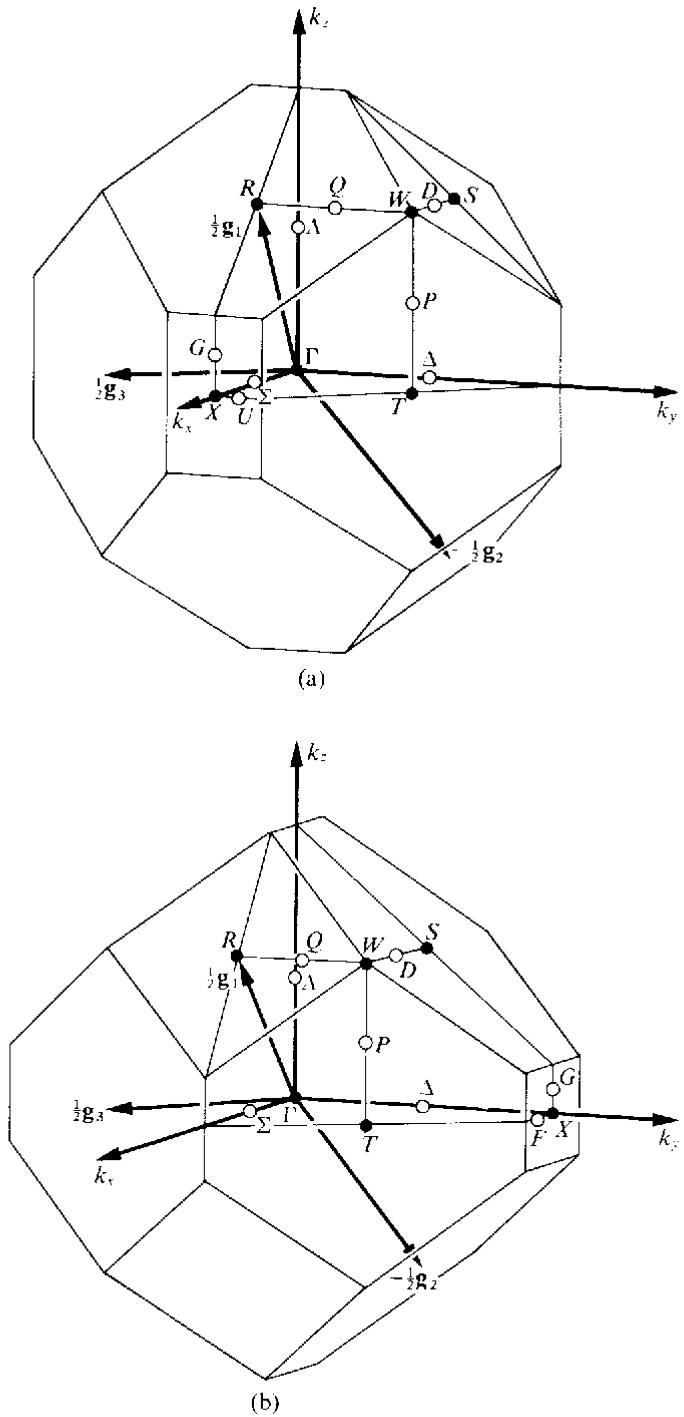
\includegraphics[width=0.62\textwidth]{fig3_7ab_mu.jpg}\\[1ex]
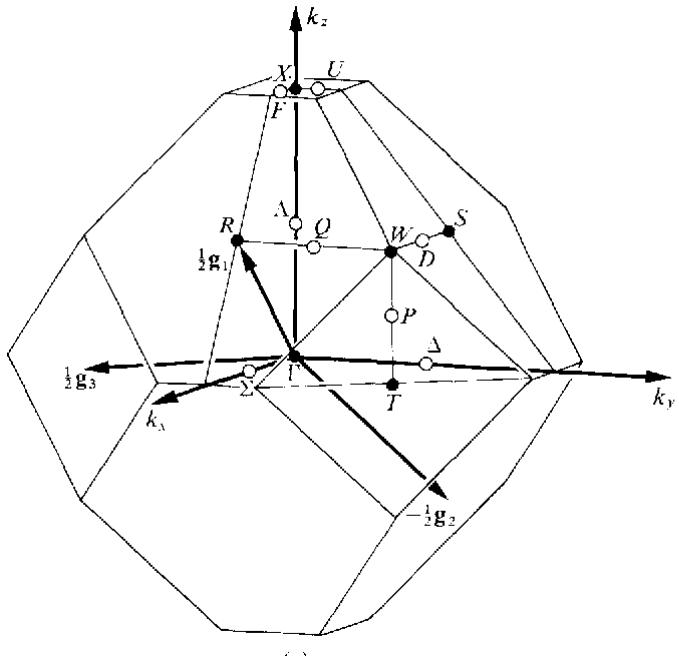
\includegraphics[width=0.62\textwidth]{fig3_7c_mu.jpg}
\caption*{\textbf{图 3.7}\ $\Gamma_{o}^{v}$（正交 $I$）的布里渊区：(a) $a>b>c$ 或 $a>c>b$，$\Gamma=(000)$；$X=(\frac{1}{2}\bar{\frac{1}{2}}\frac{1}{2})$；$R=(\bar{\frac{1}{2}}00)$；$S=(\frac{1}{2}0\bar{\frac{1}{2}})$；$T=(\frac{1}{2}\bar{\frac{1}{2}}0)$；$W=(\frac{3}{4}\bar{\frac{1}{2}}\frac{3}{4})$；(b) $b>a>c$ 或 $b>c>a$，$\Gamma=(000)$；$X=(\frac{1}{2}\frac{1}{2}\bar{\frac{1}{2}})$；$R=(\bar{\frac{1}{2}}00)$；$S=(\frac{1}{2}0\bar{\frac{1}{2}})$；$T=(\frac{1}{2}\bar{\frac{1}{2}}0)$；$W=(\frac{3}{4}\bar{\frac{1}{2}}\frac{3}{4})$；(c) $c>b>a$ 或 $c>a>b$，$\Gamma=(000)$；$X=(\frac{1}{2}\bar{\frac{1}{2}}\frac{1}{2})$；$R=(\bar{\frac{1}{2}}00)$；$S=(\frac{1}{2}0\bar{\frac{1}{2}})$；$T=(\frac{1}{2}\bar{\frac{1}{2}}0)$；$W=(\frac{3}{4}\bar{\frac{1}{2}}\frac{3}{4})$。}
\end{figure}
\begin{figure}[H]
\centering
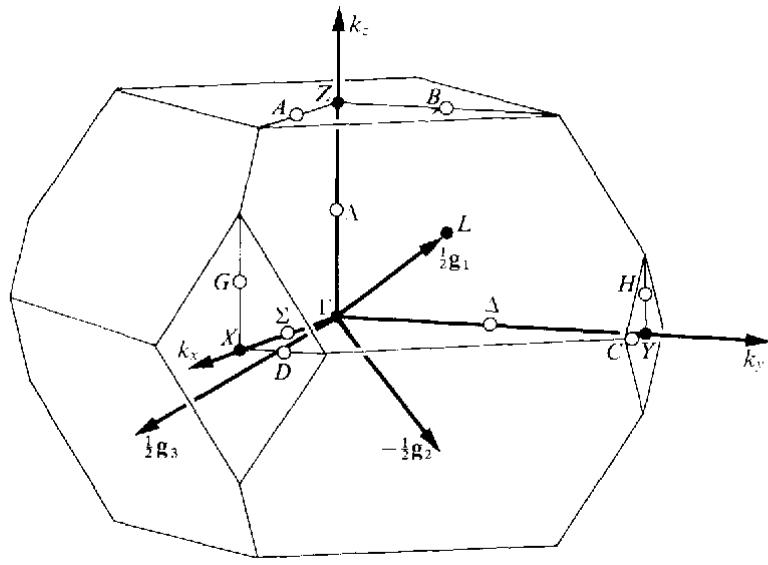
\includegraphics[width=0.60\textwidth]{fig3_8a_mu.jpg}\\[1ex]
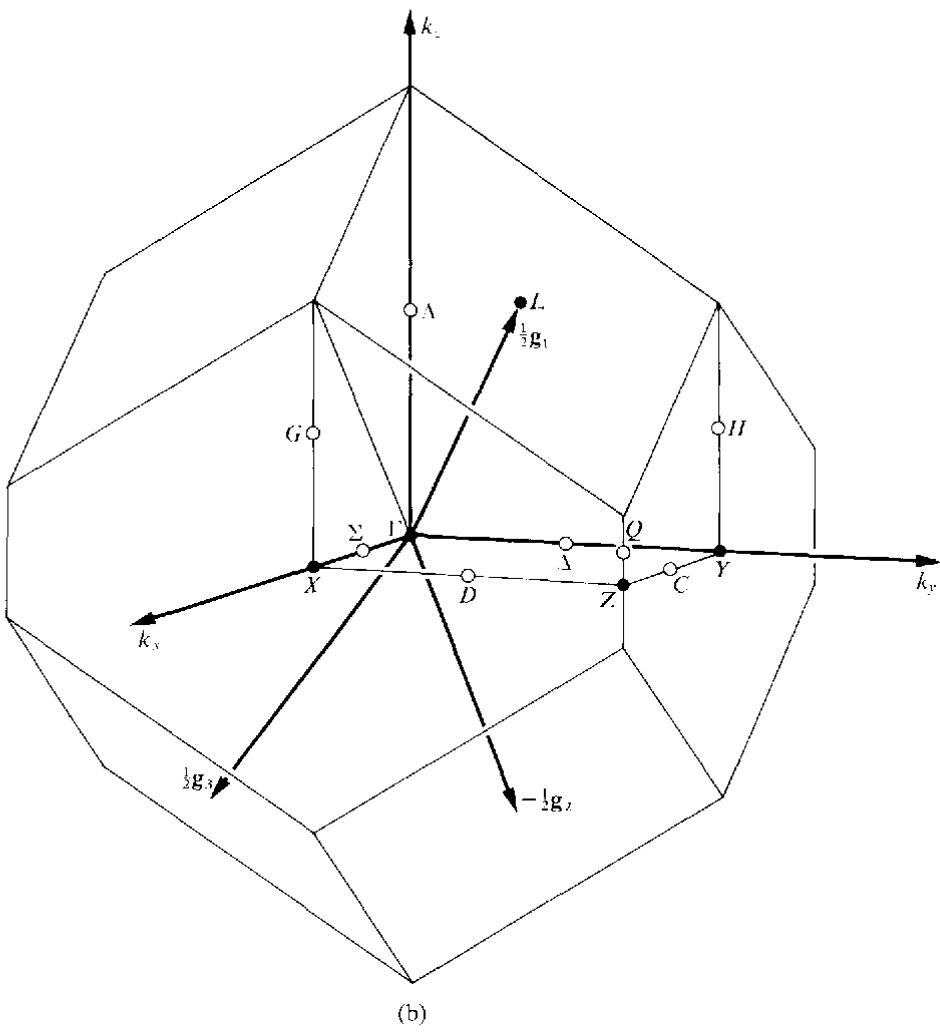
\includegraphics[width=0.60\textwidth]{fig3_8b_mu.jpg}\\[1ex]
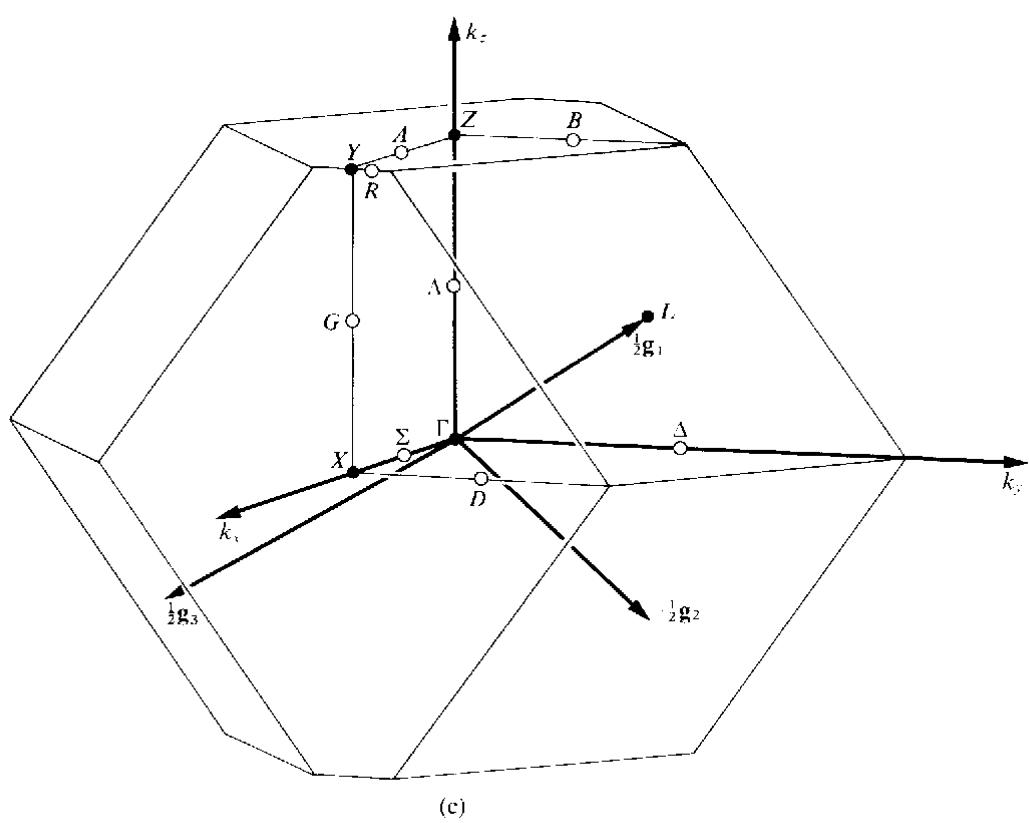
\includegraphics[width=0.60\textwidth]{fig3_8c_mu.jpg}\\[1ex]
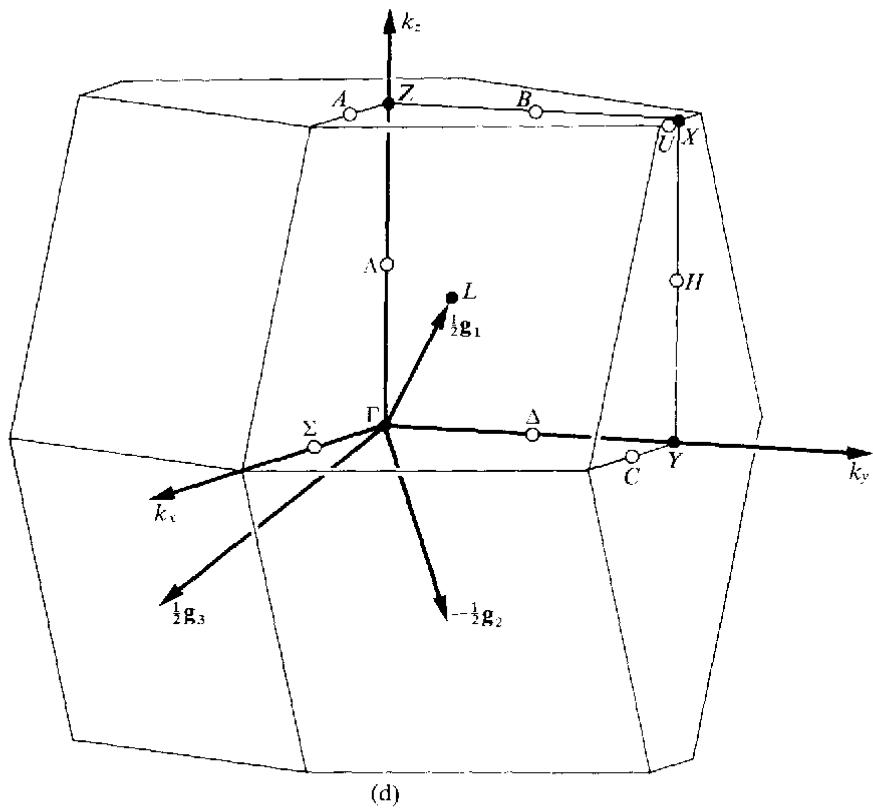
\includegraphics[width=0.60\textwidth]{fig3_8d_mu.jpg}
\caption*{\textbf{图 3.8}\ $\Gamma_{o}^{f}$（正交 $F$）的布里渊区：(a) $1/a^{2}<1/b^{2}+1/c^{2}$、$1/b^{2}<1/c^{2}+1/a^{2}$ 且 $1/c^{2}<1/a^{2}+1/b^{2}$，$\Gamma=(000)$；$Y=(0\bar{\frac{1}{2}}\frac{1}{2})$；$X=(\frac{1}{2}0\frac{1}{2})$；$Z=(\frac{1}{2}\bar{\frac{1}{2}}0)$；$L=(\frac{1}{4}00)$；(b) $1/c^{2}>1/a^{2}+1/b^{2}$，$\Gamma=(000)$；$Y=(0\bar{\frac{1}{2}}\frac{1}{2})$；$X=(\frac{1}{2}0\frac{1}{2})$；$Z=(\frac{1}{2}\bar{\frac{1}{2}}0)$；$L=(\frac{1}{4}00)$；(c) $1/b^{2}>1/a^{2}+1/c^{2}$，$\Gamma=(000)$；$Y=(1\bar{\frac{1}{2}}\frac{1}{2})$；$X=(\frac{1}{2}0\frac{1}{2})$；$Z=(\frac{1}{2}\bar{\frac{1}{2}}0)$；$L=(\frac{1}{4}00)$；(d) $1/a^{2}>1/b^{2}+1/c^{2}$，$\Gamma=(000)$；$Y=(0\bar{\frac{1}{2}}\frac{1}{2})$；$X=(\frac{1}{2}0\frac{1}{2})$；$Z=(\frac{1}{2}\frac{1}{2}0)$；$L=(\frac{1}{4}00)$。}
\end{figure}
\begin{figure}[H]
\centering
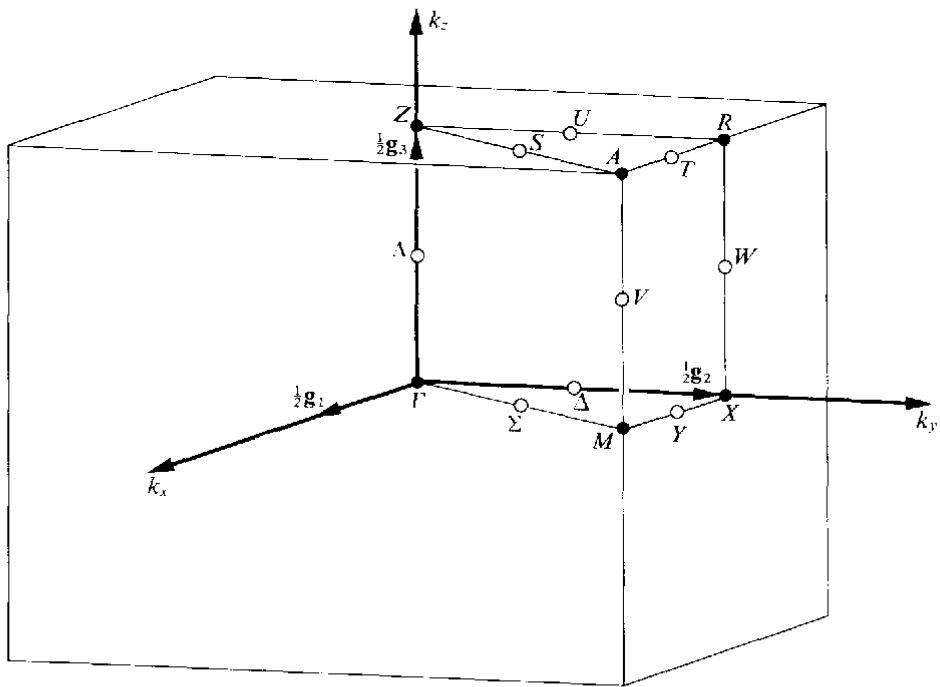
\includegraphics[width=0.60\textwidth]{fig3_9_mu.jpg}
\caption*{\textbf{图 3.9}\ $\Gamma_{q}$（四方 $P$）的布里渊区。$\Gamma=(000)$；$M=(\frac{1}{2}\frac{1}{2}0)$；$Z=(00\frac{1}{2})$；$A=(\frac{1}{2}\frac{1}{2}\frac{1}{2})$；$R=(0\frac{1}{2}\frac{1}{2})$；$X=(0\frac{1}{2}0)$。}
\end{figure}
\begin{figure}[H]
\centering
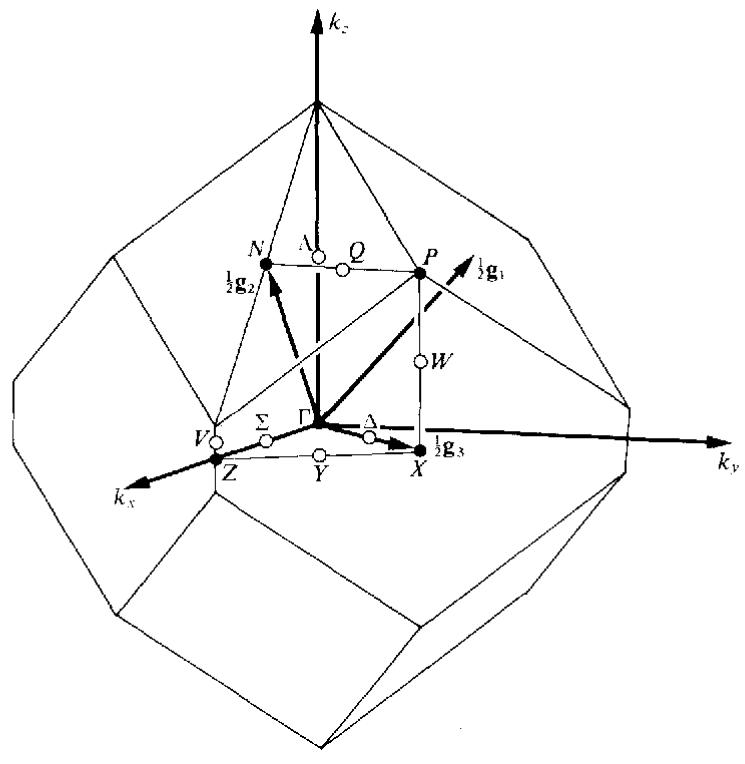
\includegraphics[width=0.60\textwidth]{fig3_10a_mu.jpg}\\[1ex]
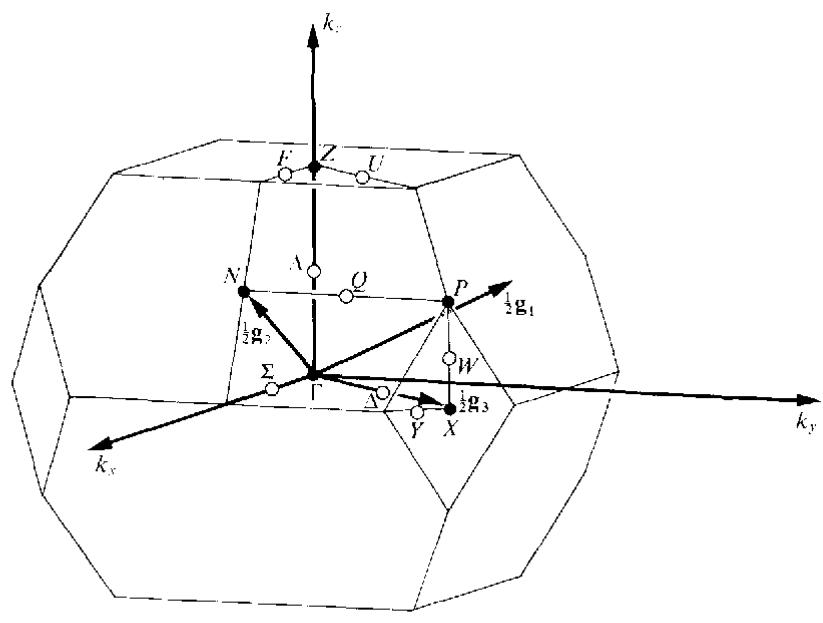
\includegraphics[width=0.60\textwidth]{fig3_10b_mu.jpg}
\caption*{\textbf{图 3.10}\ $\Gamma_{q}^{v}$（四方 $I$）的布里渊区：(a) $a>c$；(b) $c>a$。两种情形都有 $\Gamma=(000)$；$N=(0\frac{1}{2}0)$；$X=(00\frac{1}{2})$；$Z=(\bar{\frac{1}{2}}\bar{\frac{1}{2}}\bar{\frac{1}{2}})$；$P=(\frac{1}{4}\frac{1}{4}\frac{1}{4})$。}
\end{figure}
\begin{figure}[H]
\centering
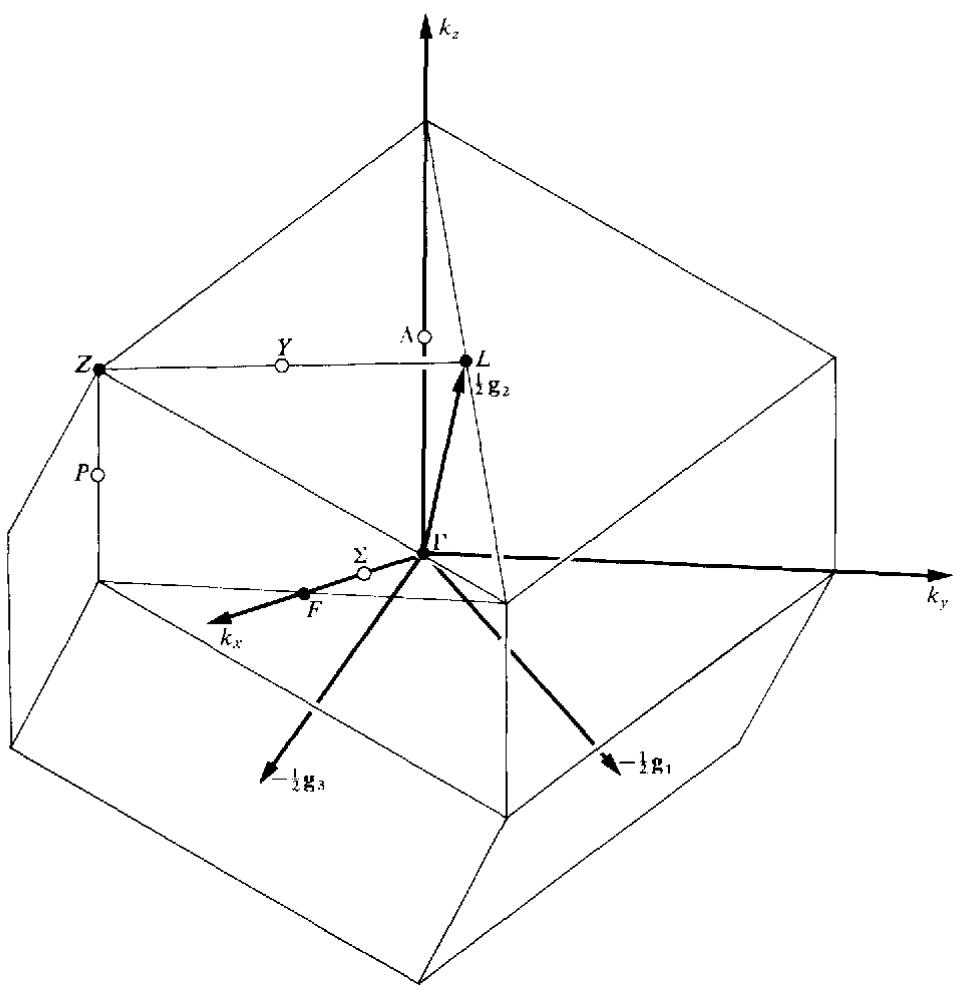
\includegraphics[width=0.60\textwidth]{fig3_11a_mu.jpg}\\[1ex]
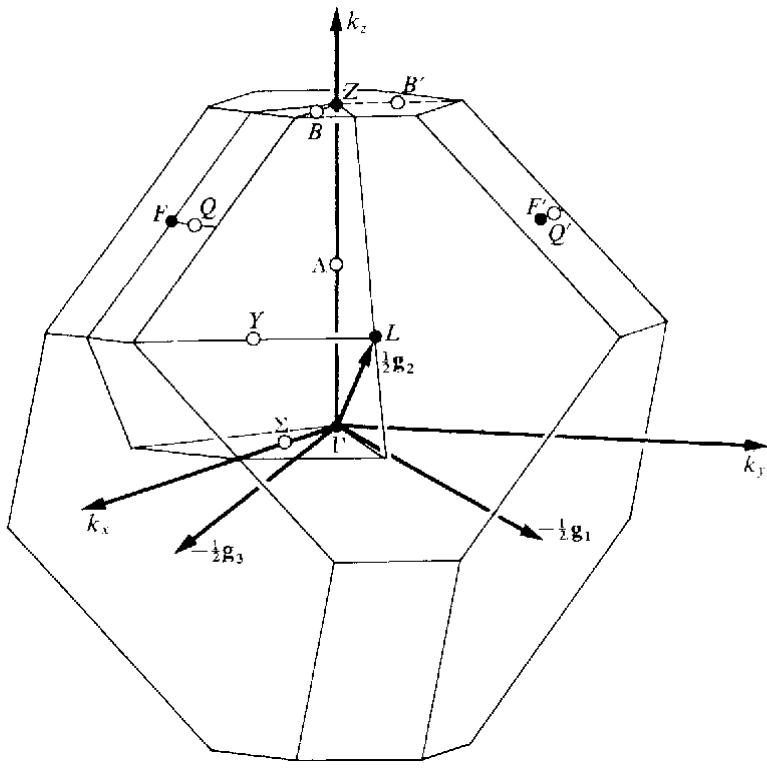
\includegraphics[width=0.60\textwidth]{fig3_11b_mu.jpg}
\caption*{\textbf{图 3.11}\ $\Gamma_{rh}$（三方 $R$）的布里渊区：(a) $a>\sqrt{2}\,c$，$\Gamma=(000)$；$Z=(\frac{1}{2}\frac{1}{2}\bar{\frac{1}{2}})$；$L=(0\frac{1}{2}0)$；$F=(0\frac{1}{2}\bar{\frac{1}{2}})$；(b) $\sqrt{2}\,c>a$，$\Gamma=(000)$；$Z=(\frac{1}{2}\frac{1}{2}\frac{1}{2})$；$L=(0\frac{1}{2}0)$；$F=(\frac{1}{2}\frac{1}{2}0)$。在 (a) 中 $\Sigma$ 和 $Y$ 是两条完整的对称线；在 (b) 中 $Q$ 和 $B$ 经过一个三次转动分别与 $Q'$ 和 $B'$ 相关联，二者分别是线 $\Sigma$ 和 $Y$ 的延续（$F'=(0\bar{\frac{1}{2}}\bar{\frac{1}{2}})$，由 $F$ 经三次转动得到；另见表 3.6）。}
\end{figure}
\begin{figure}[H]
\centering
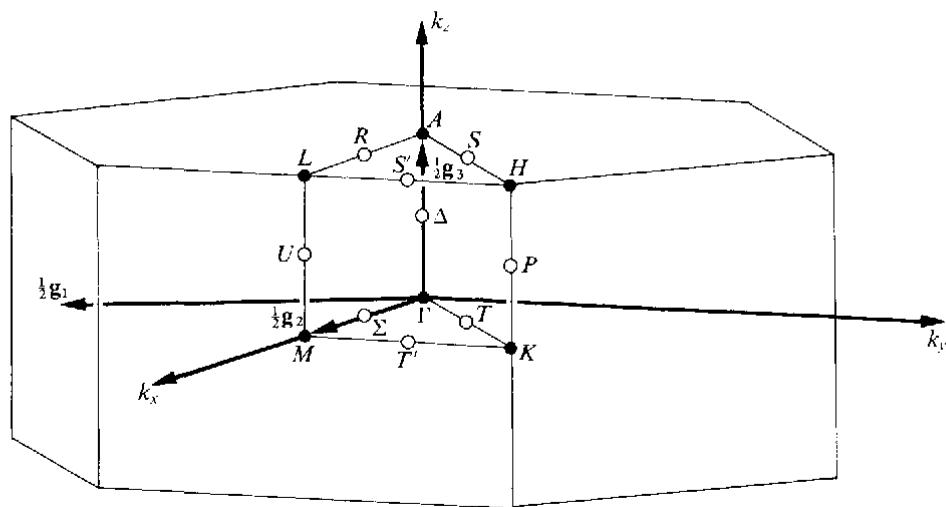
\includegraphics[width=0.60\textwidth]{fig3_12_mu.jpg}
\caption*{\textbf{图 3.12}\ $\Gamma_{h}$（六角 $P$）的布里渊区。$\Gamma=(000)$；$M=(0\frac{1}{2}0)$；$A=(00\frac{1}{2})$；$L=(0\frac{1}{2}\frac{1}{2})$；$K=(\bar{\frac{1}{3}}\frac{2}{3}0)$；$H=(\bar{\frac{1}{3}}\frac{2}{3}\frac{1}{2})$。}
\end{figure}
\begin{figure}[H]
\centering
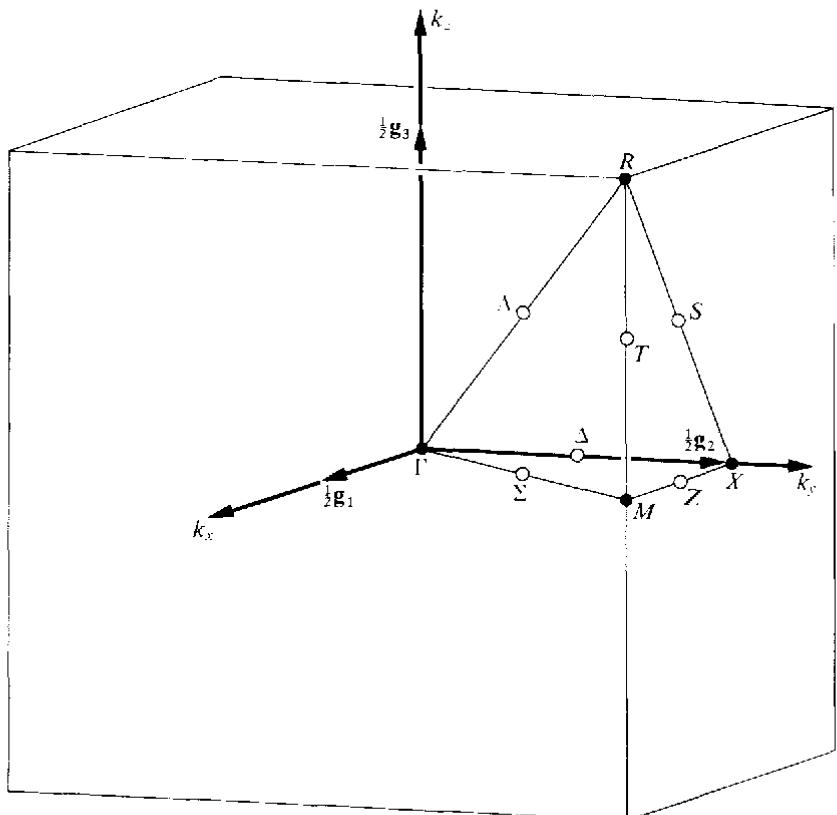
\includegraphics[width=0.58\textwidth]{fig3_13_mu.jpg}
\caption*{\textbf{图 3.13}\ $\Gamma_{c}$（立方 $P$）的布里渊区。$\Gamma=(000)$；$X=(0\frac{1}{2}0)$；$M=(\frac{1}{2}\frac{1}{2}0)$；$R=(\frac{1}{2}\frac{1}{2}\frac{1}{2})$。}
\end{figure}
\begin{figure}[H]
\centering
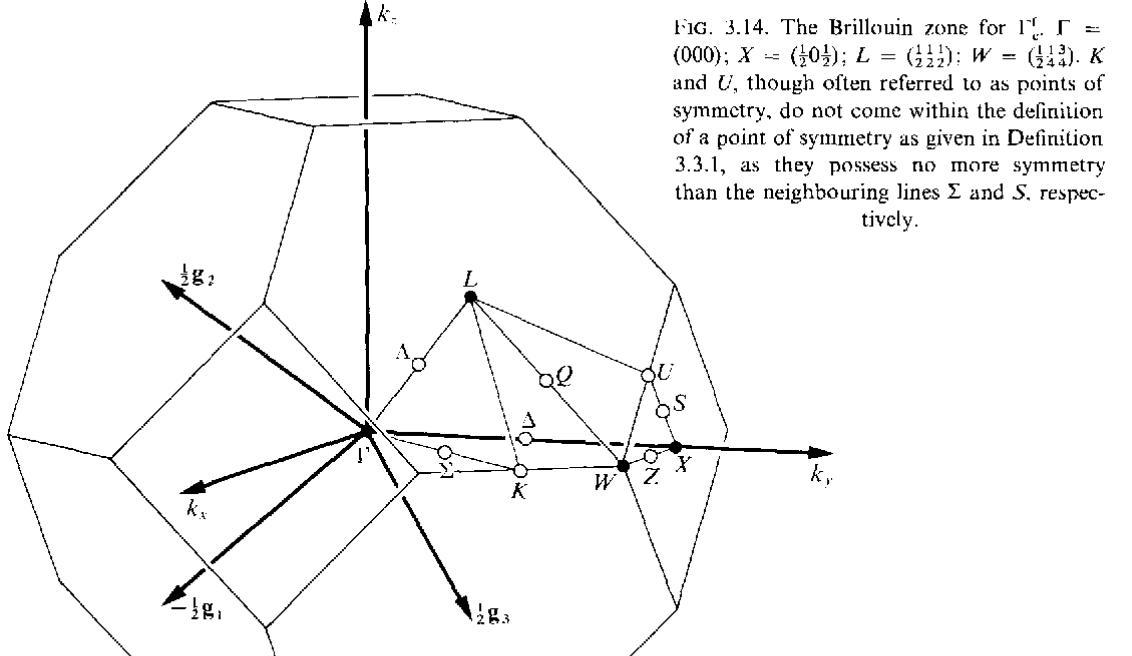
\includegraphics[width=0.58\textwidth]{fig3_14_mu.jpg}
\caption*{\textbf{图 3.14}\ $\Gamma_{c}^{f}$（立方 $F$）的布里渊区。$\Gamma=(000)$；$X=(\frac{1}{2}0\frac{1}{2})$；$L=(\frac{1}{2}\frac{1}{2}\frac{1}{2})$；$W=(\frac{1}{2}\frac{1}{4}\frac{3}{4})$。$K$ 和 $U$ 虽常被称为对称点，但按定义 3.3.1 它们并不算对称点，因为它们并不比相邻的线 $\Sigma$ 和 $S$ 具有更多对称性。}
\end{figure}
\begin{figure}[H]
\centering
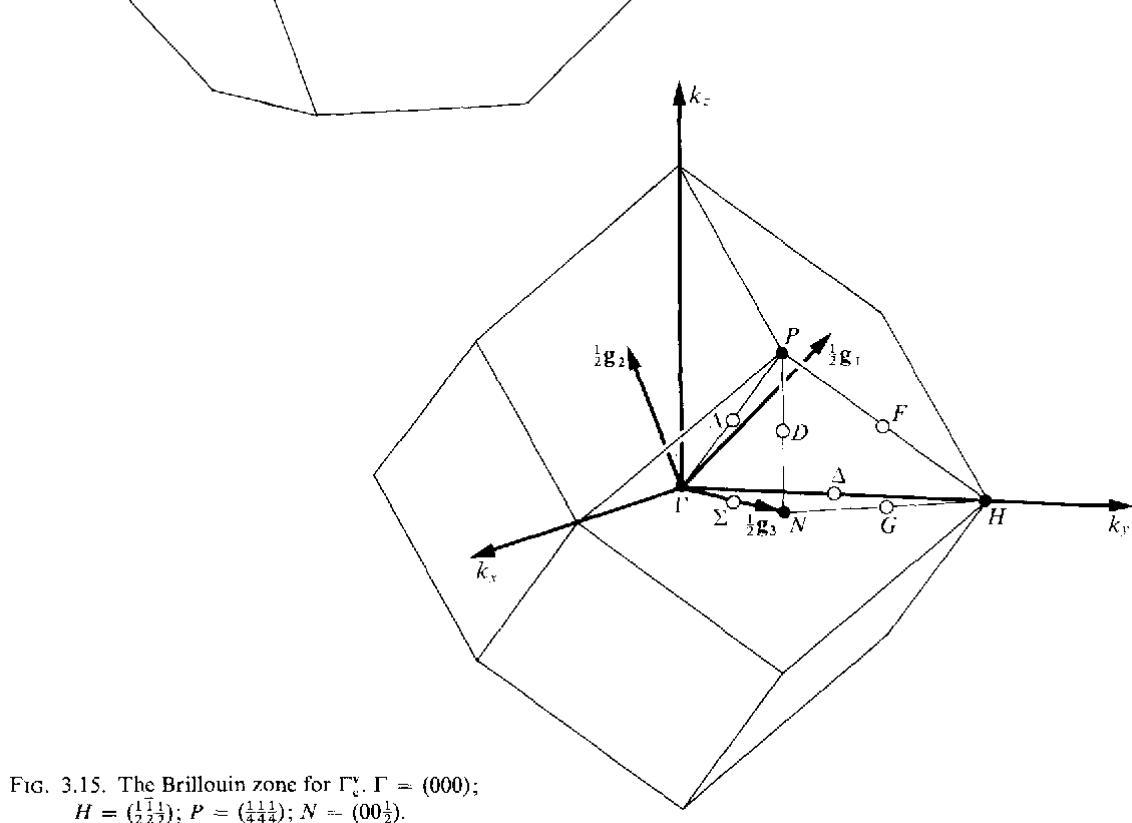
\includegraphics[width=0.56\textwidth]{fig3_15_mu.jpg}
\caption*{\textbf{图 3.15}\ $\Gamma_{c}^{v}$（立方 $I$）的布里渊区。$\Gamma=(000)$；$H=(\frac{1}{2}\frac{1}{2}\frac{1}{2})$；$P=(\frac{1}{4}\frac{1}{4}\frac{1}{4})$；$N=(00\frac{1}{2})$。}
\end{figure}

对某些布拉维格子，布里渊区的形状是唯一的，例如三种立方布拉维格子（其布里渊区绘于图 3.13--3.15）。但对另外一些布拉维格子，可能出现的形状不止一种，取决于布拉维格子的轴比和轴间角。对三斜布拉维格子（图 3.2）和两种单斜布拉维格子（图 3.3、3.4），我们遵循定义 3.2.2，用倒空间的初基晶胞来定义布里渊区。对另一些布拉维格子，可能出现表面上不同的布里渊区（例如图 3.8 的 $\Gamma_{o}^{f}$、图 3.10 的 $\Gamma_{q}^{v}$、图 3.11 的 $\Gamma_{rh}$）。然而，当可能有两个表面上不同的布里渊区时，每种情形中对称点的数目是相同的。例如在图 3.11(a)（$\Gamma_{rh}$，$a>\sqrt{2}\,c$）中，对称点是 $\Gamma$（$\mathbf{k}=0$）、$L$（$\mathbf{k}=\frac{1}{2}\mathbf{g}_{2}$）、$F$（$\mathbf{k}=\frac{1}{2}\mathbf{g}_{2}-\frac{1}{2}\mathbf{g}_{3}$）和 $Z$（$\mathbf{k}=\frac{1}{2}\mathbf{g}_{1}+\frac{1}{2}\mathbf{g}_{2}-\frac{1}{2}\mathbf{g}_{3}$）；而在图 3.11(b) 的替代布里渊区（$a<\sqrt{2}\,c$）中，对称点是 $\Gamma$（$\mathbf{k}=0$）、$L$（$\mathbf{k}=\frac{1}{2}\mathbf{g}_{2}$）、$F$（$\mathbf{k}=\frac{1}{2}\mathbf{g}_{1}+\frac{1}{2}\mathbf{g}_{2}$）和 $Z$（$\mathbf{k}=\frac{1}{2}\mathbf{g}_{1}+\frac{1}{2}\mathbf{g}_{2}+\frac{1}{2}\mathbf{g}_{3}$）。$\Gamma$ 和 $L$ 在两个布里渊区中以相同的 $\mathbf{k}$ 出现，而图 3.11(a) 中的 $F$ 和 $Z$ 在图 3.11(b) 中对应的 $\mathbf{k}$ 矢量不同但等价。对另外一些布拉维格子，布里渊区的外形相同，只是各面相对 $k_{x}$、$k_{y}$、$k_{z}$ 轴的取向不同，见图 3.16。

\begin{figure}[H]
\centering
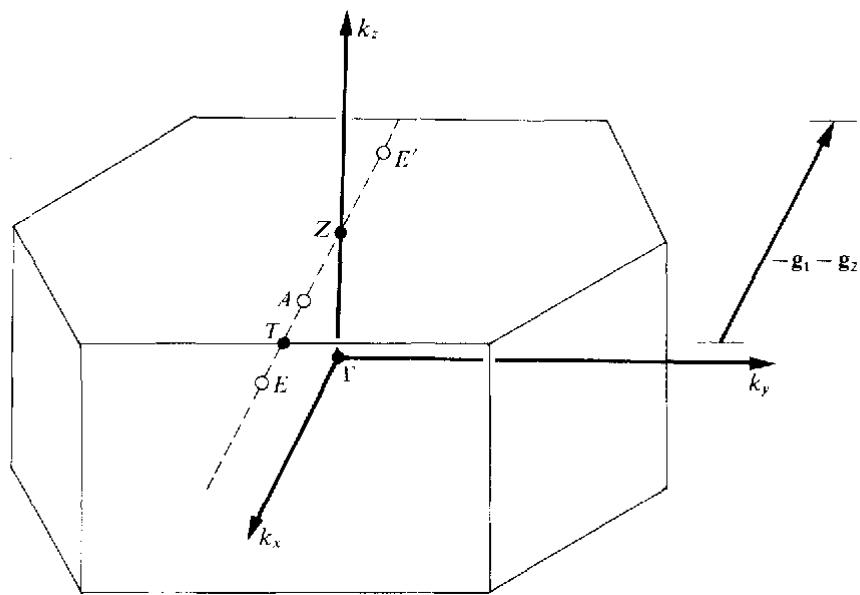
\includegraphics[width=0.56\textwidth]{fig3_16_mu.jpg}
\caption*{\textbf{图 3.16}\ $\Gamma_{o}^{b}$ 的布里渊区。}
\end{figure}

考虑 $\Gamma_{o}^{b}$（图 3.6）。当 $a>b$ 时（图 3.6(a)），设 $T$ 是线 $ZT$ 上的一个点，其 $\mathbf{k}$ 矢量为 $\mathbf{k}_{T}$，则
\begin{equation*}
\mathbf{k}_{E} = \mathbf{k}_{T} + (\alpha\mathbf{g}_{1} + \alpha\mathbf{g}_{2}).
\tag{3.3.2}
\end{equation*}
图 3.6(a) 中相应的对称线具有由式 (3.3.2) 给出的 $\mathbf{k}$ 矢量 $\mathbf{k}_{E}$，即线 $ZT$ 的延续；见图 3.16。这条线 $E$ 现在已跑到第一布里渊区之外，但它等价于第一区内的一条线，即 $E'$，其中
\begin{equation*}
\mathbf{k}_{E'} = \mathbf{k}_{E} - \mathbf{g}_{1} - \mathbf{g}_{2}.
\tag{3.3.3}
\end{equation*}
线 $E'$ 与图 3.6(a) 中的线 $A$ 有简单的对称关系，因此不必把它同 $A$ 分开考虑。反过来看，这意味着图 3.6(a) 中的线 $A$ 在图 3.6(b) 中被分成两段：对某些 $\alpha$ 值的一段是图 3.6(a) 的 $A$，对其余 $\alpha$ 值的一段是图 3.6(b) 的 $E$。类似地，图 3.6(a) 中的线 $\Sigma$ 在图 3.6(b) 中被分成 $\Lambda$ 和 $C$。反过来，图 3.6(b) 中的线 $A$ 在图 3.6(a) 中被分成 $\Delta$ 和 $F$，而图 3.6(b) 中的线 $B$ 被分成 $\Delta$ 和 $F'$。

由于我们指出的这种等价性，在本书后面的表中，对 14 种布拉维格子中的每一种，只需对一个布里渊区列出对称点即可；通常也只需对每一种格子列出一张对称线表。不过，对区面上的对称线存在少数例外。例如，虽然图 3.6(b) 中的 $C$ 与图 3.6(a) 中的 $E$ 相关联，但二者之间存在一个微妙的差别，这将在后文变得明显。

14 种布拉维格子各自基本域中每个对称点和对称线的群 $\mathbf{P}(\mathbf{k})$（$\mathbf{k}$ 的对称群）列于表 3.6。可以注意到，图 3.2--3.15 中基本域的许多棱并不是对称线，而只是（按定义 3.3.2 的意义）对称面。把我们限制在单一基本域的理由后文自明；例如见 5.5 节。

\begin{figure}[H]
\centering
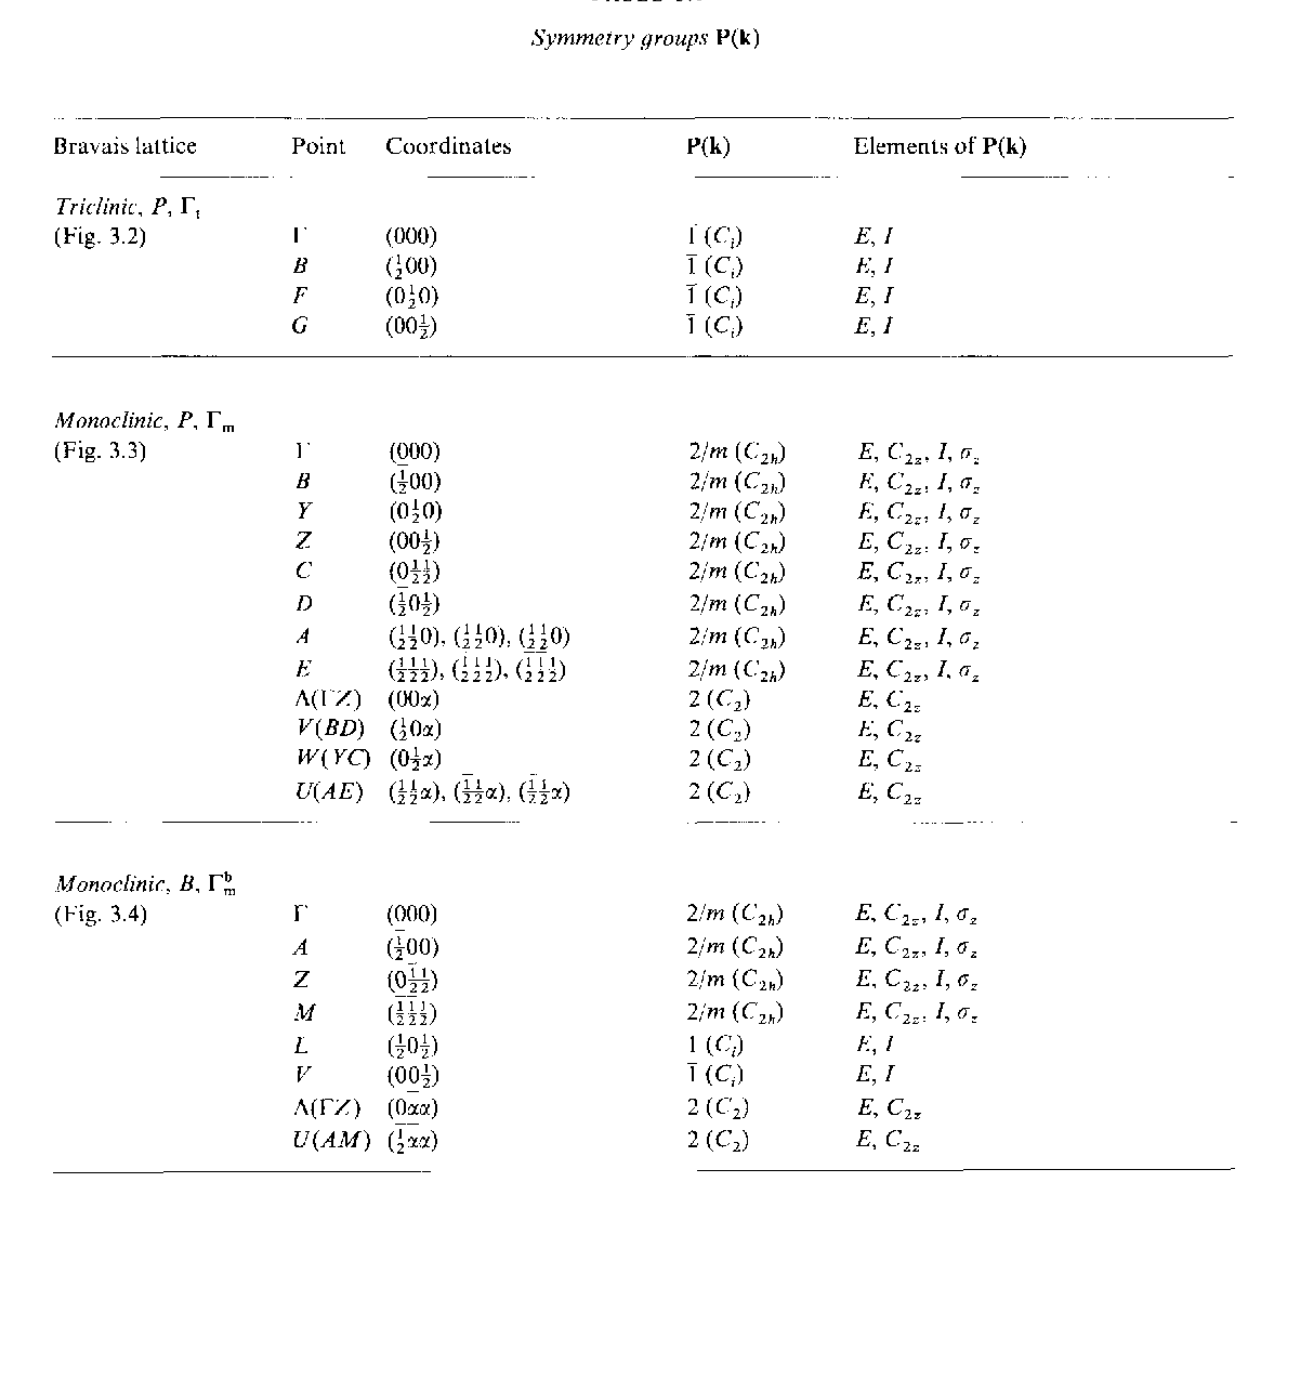
\includegraphics[width=0.92\textwidth]{c3_t36_p1.png}
\caption*{\textbf{表 3.6}\ 对称群 $\mathbf{P}(\mathbf{k})$（原书第 113 页起扫描；第 1--5 页）。}
\end{figure}
\begin{figure}[H]
\centering
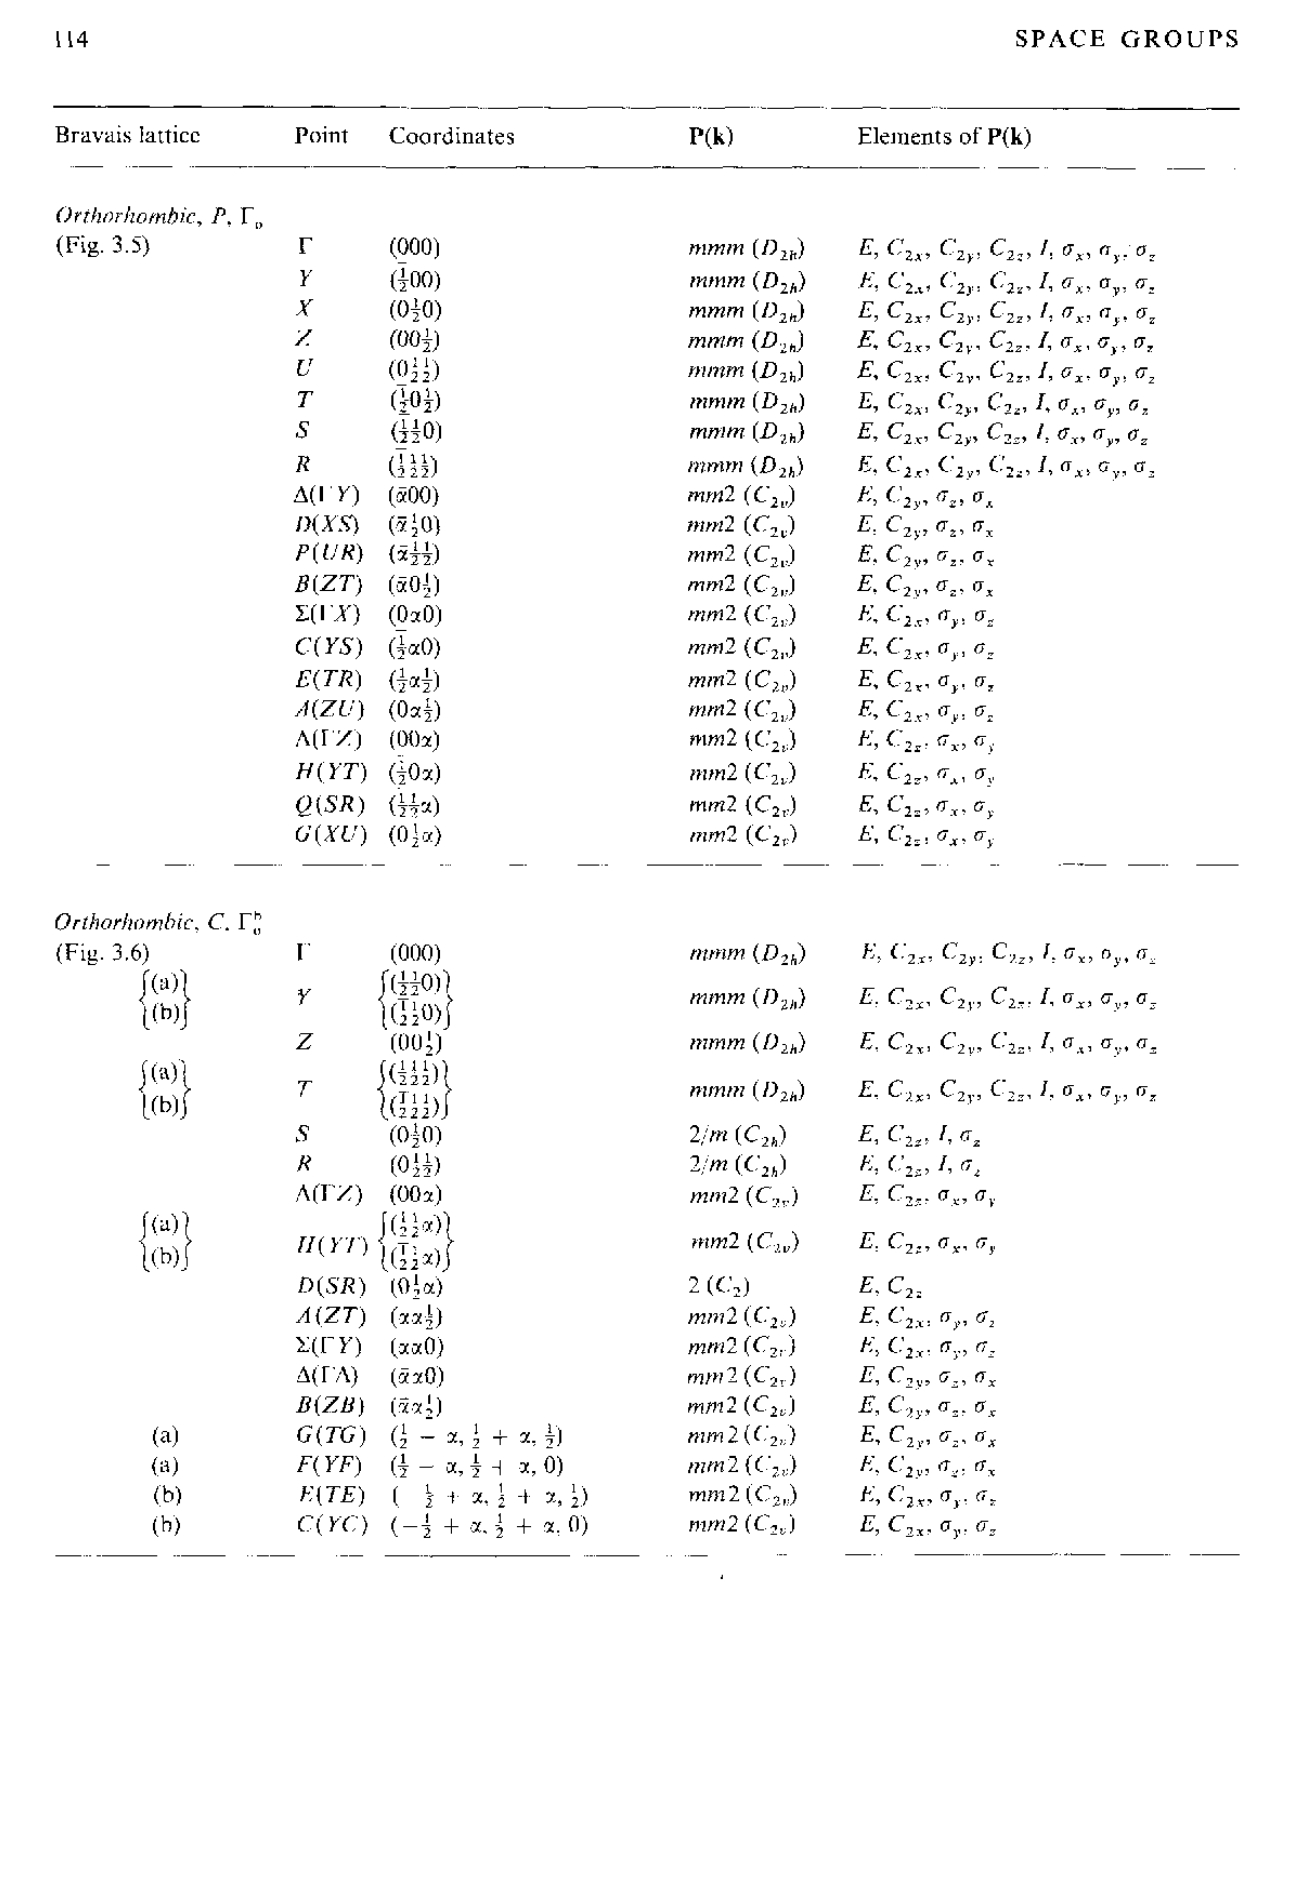
\includegraphics[width=0.92\textwidth]{c3_t36_p2.png}
\caption*{\textbf{表 3.6}（第 2 页）。}
\end{figure}
\begin{figure}[H]
\centering
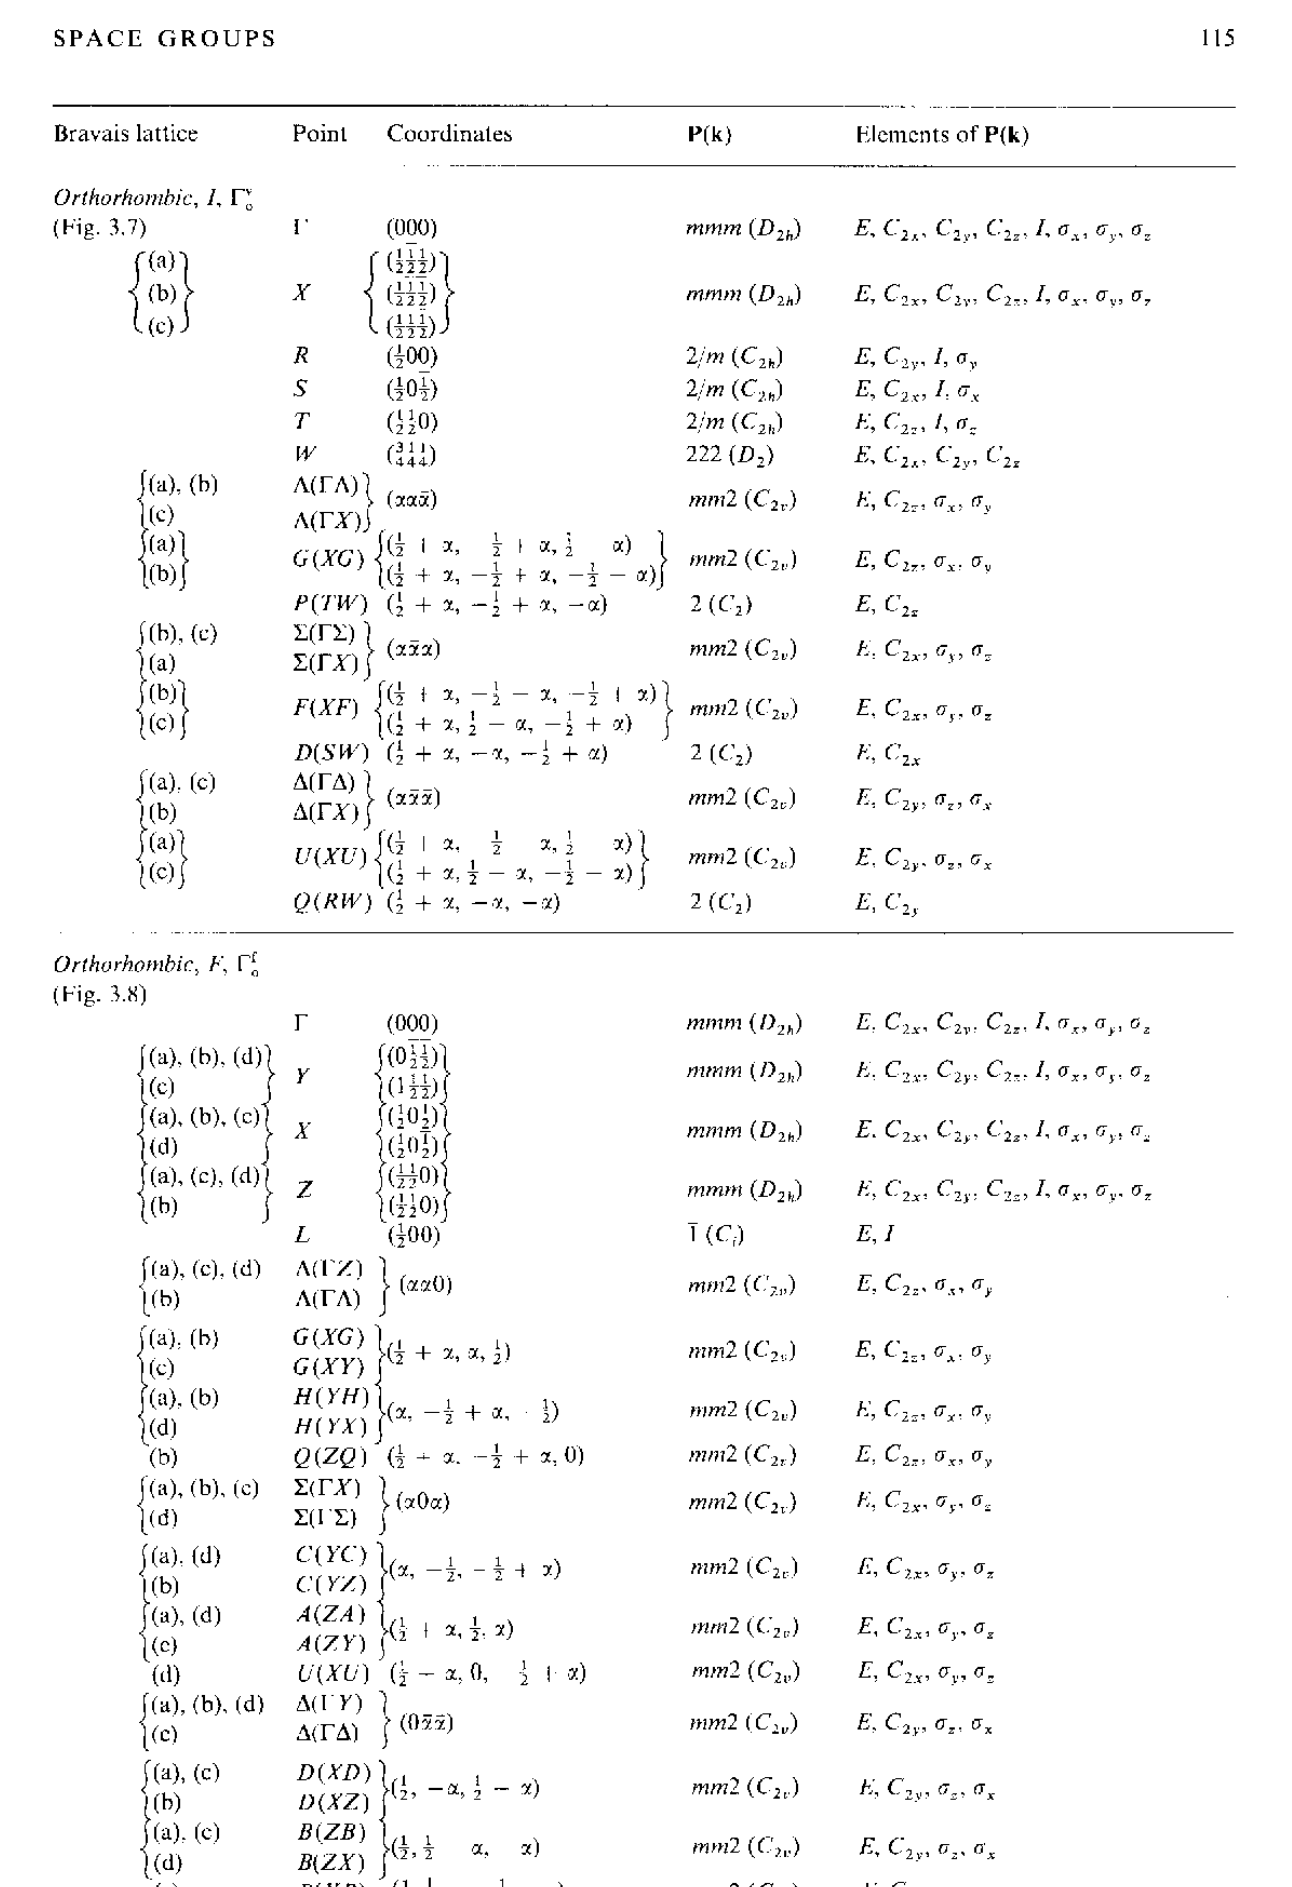
\includegraphics[width=0.92\textwidth]{c3_t36_p3.png}
\caption*{\textbf{表 3.6}（第 3 页）。}
\end{figure}
\begin{figure}[H]
\centering
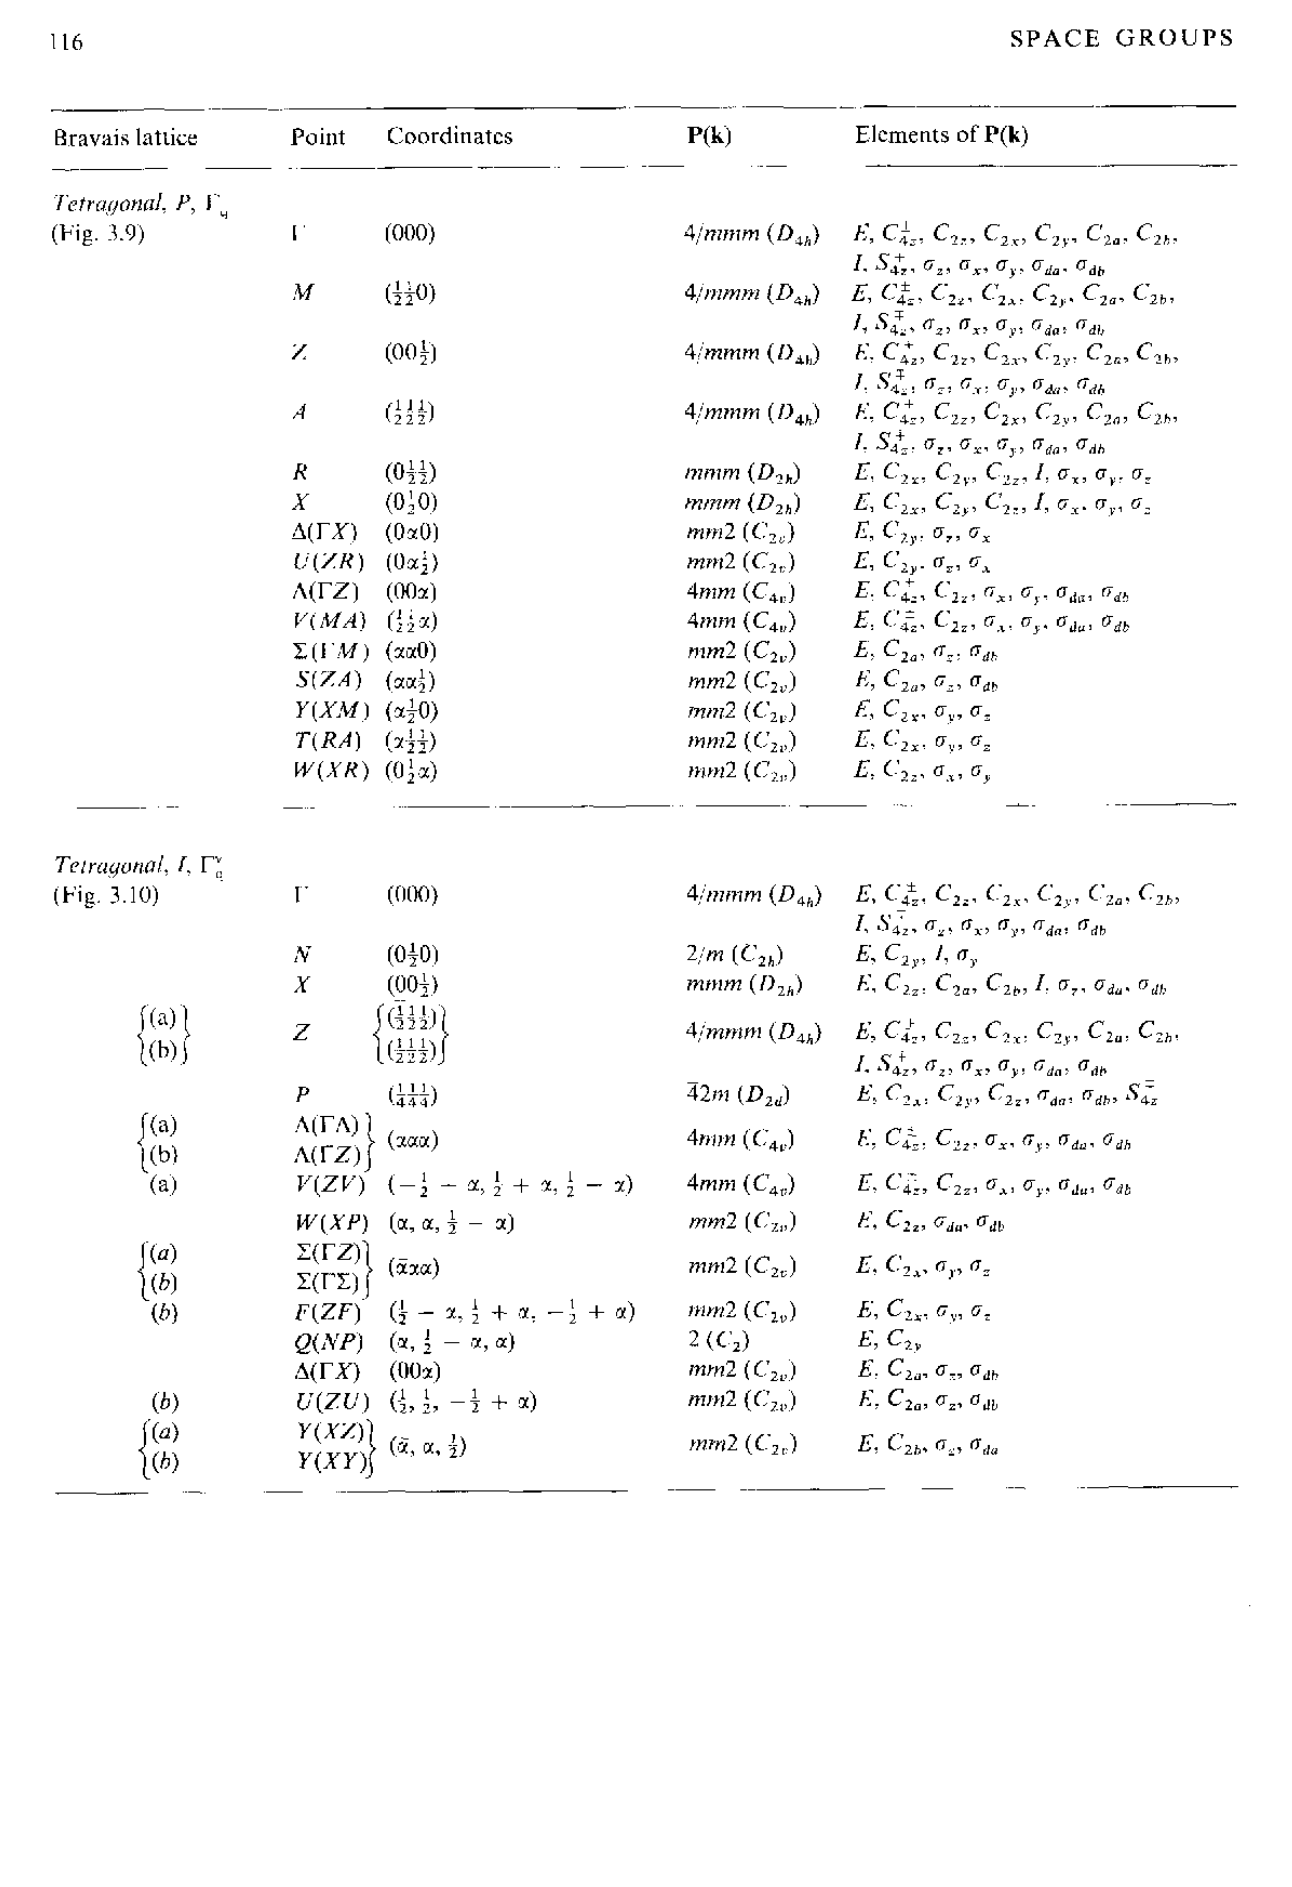
\includegraphics[width=0.92\textwidth]{c3_t36_p4.png}
\caption*{\textbf{表 3.6}（第 4 页）。}
\end{figure}
\begin{figure}[H]
\centering
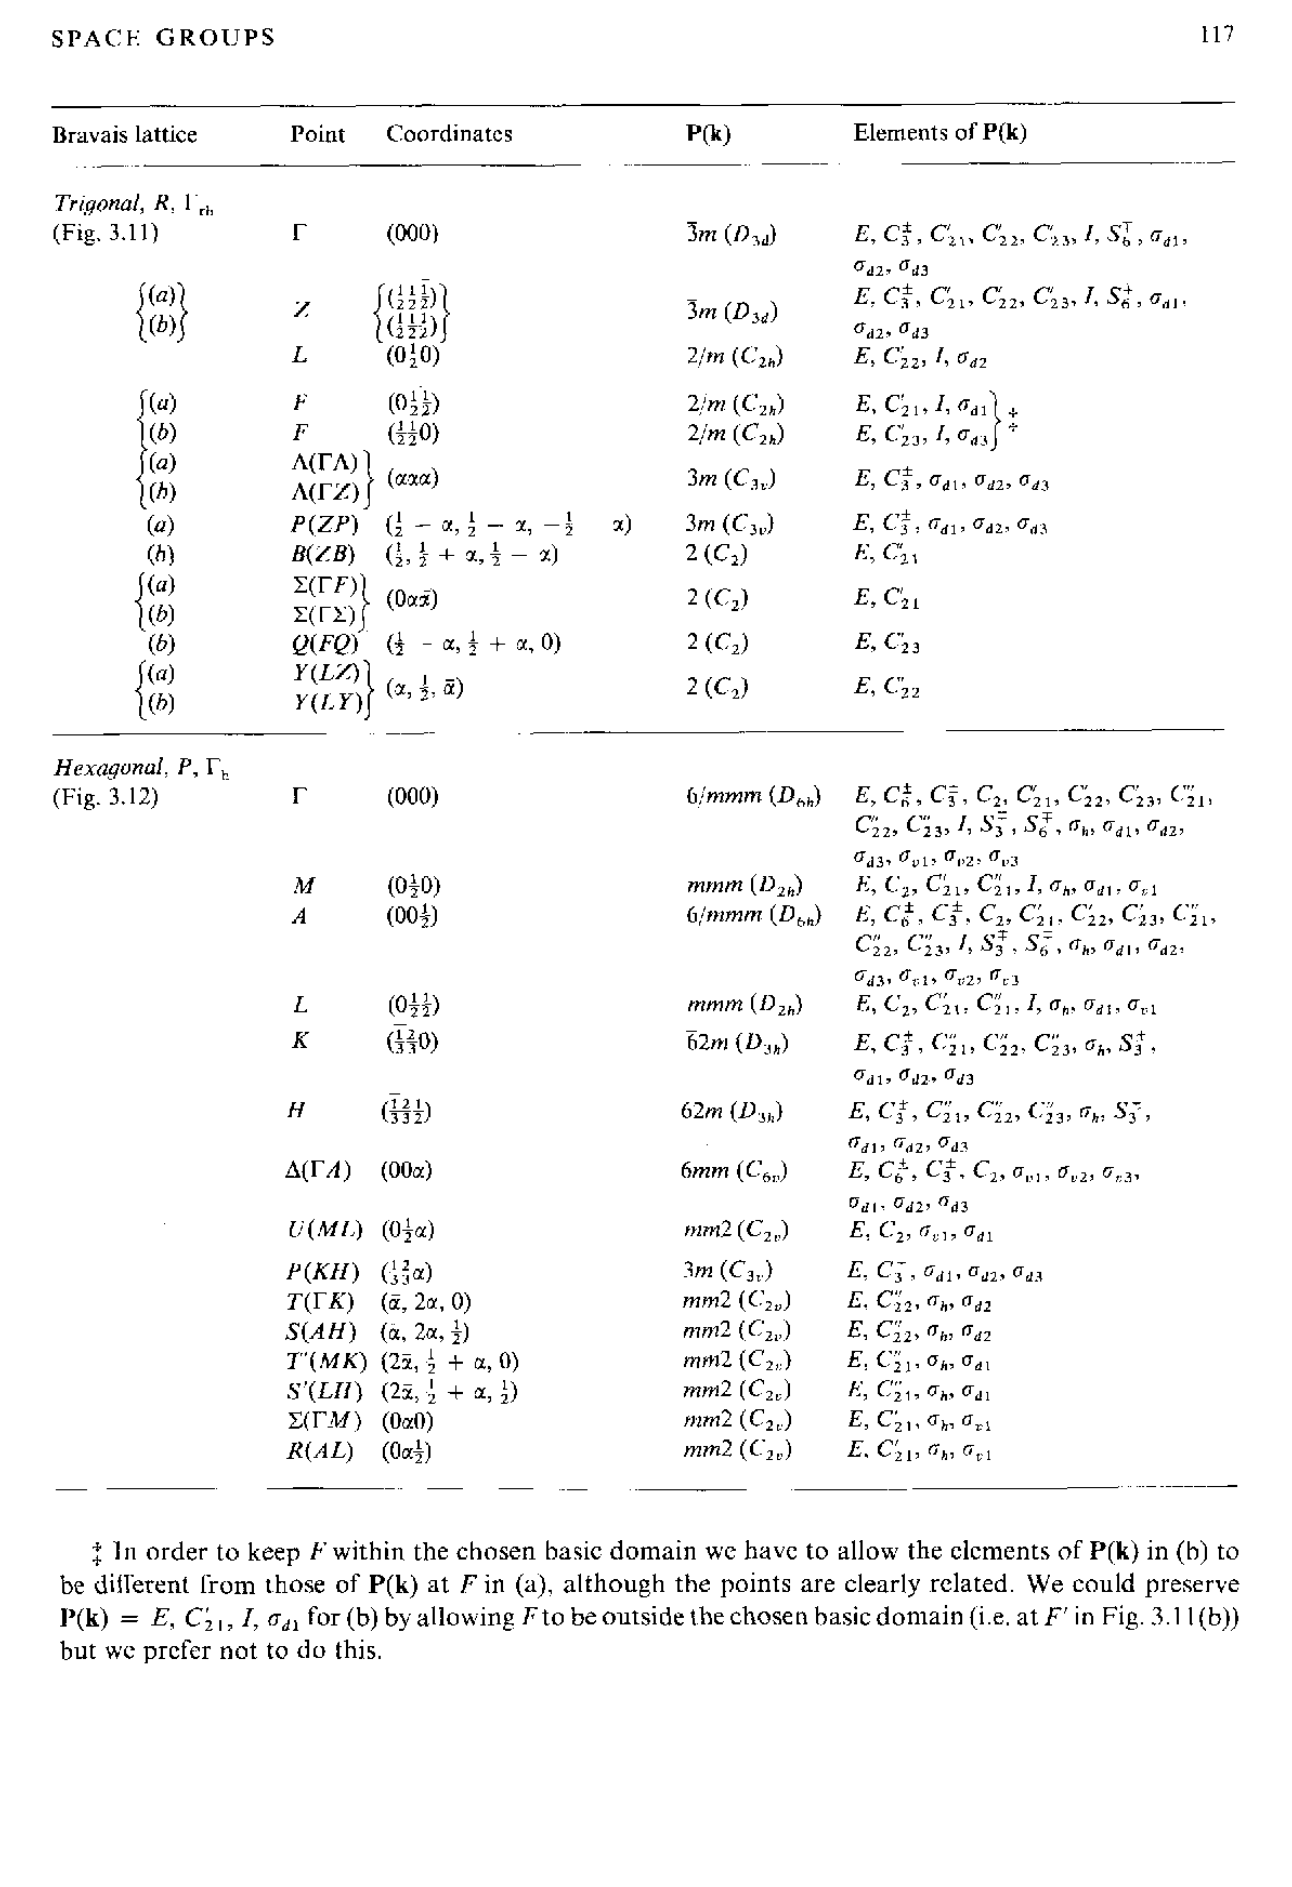
\includegraphics[width=0.92\textwidth]{c3_t36_p5.png}
\caption*{\textbf{表 3.6}（第 5 页；本页下部有关于 $\Gamma_{rh}$ 的 $F$ 点的脚注）。}
\end{figure}
\begin{figure}[H]
\centering
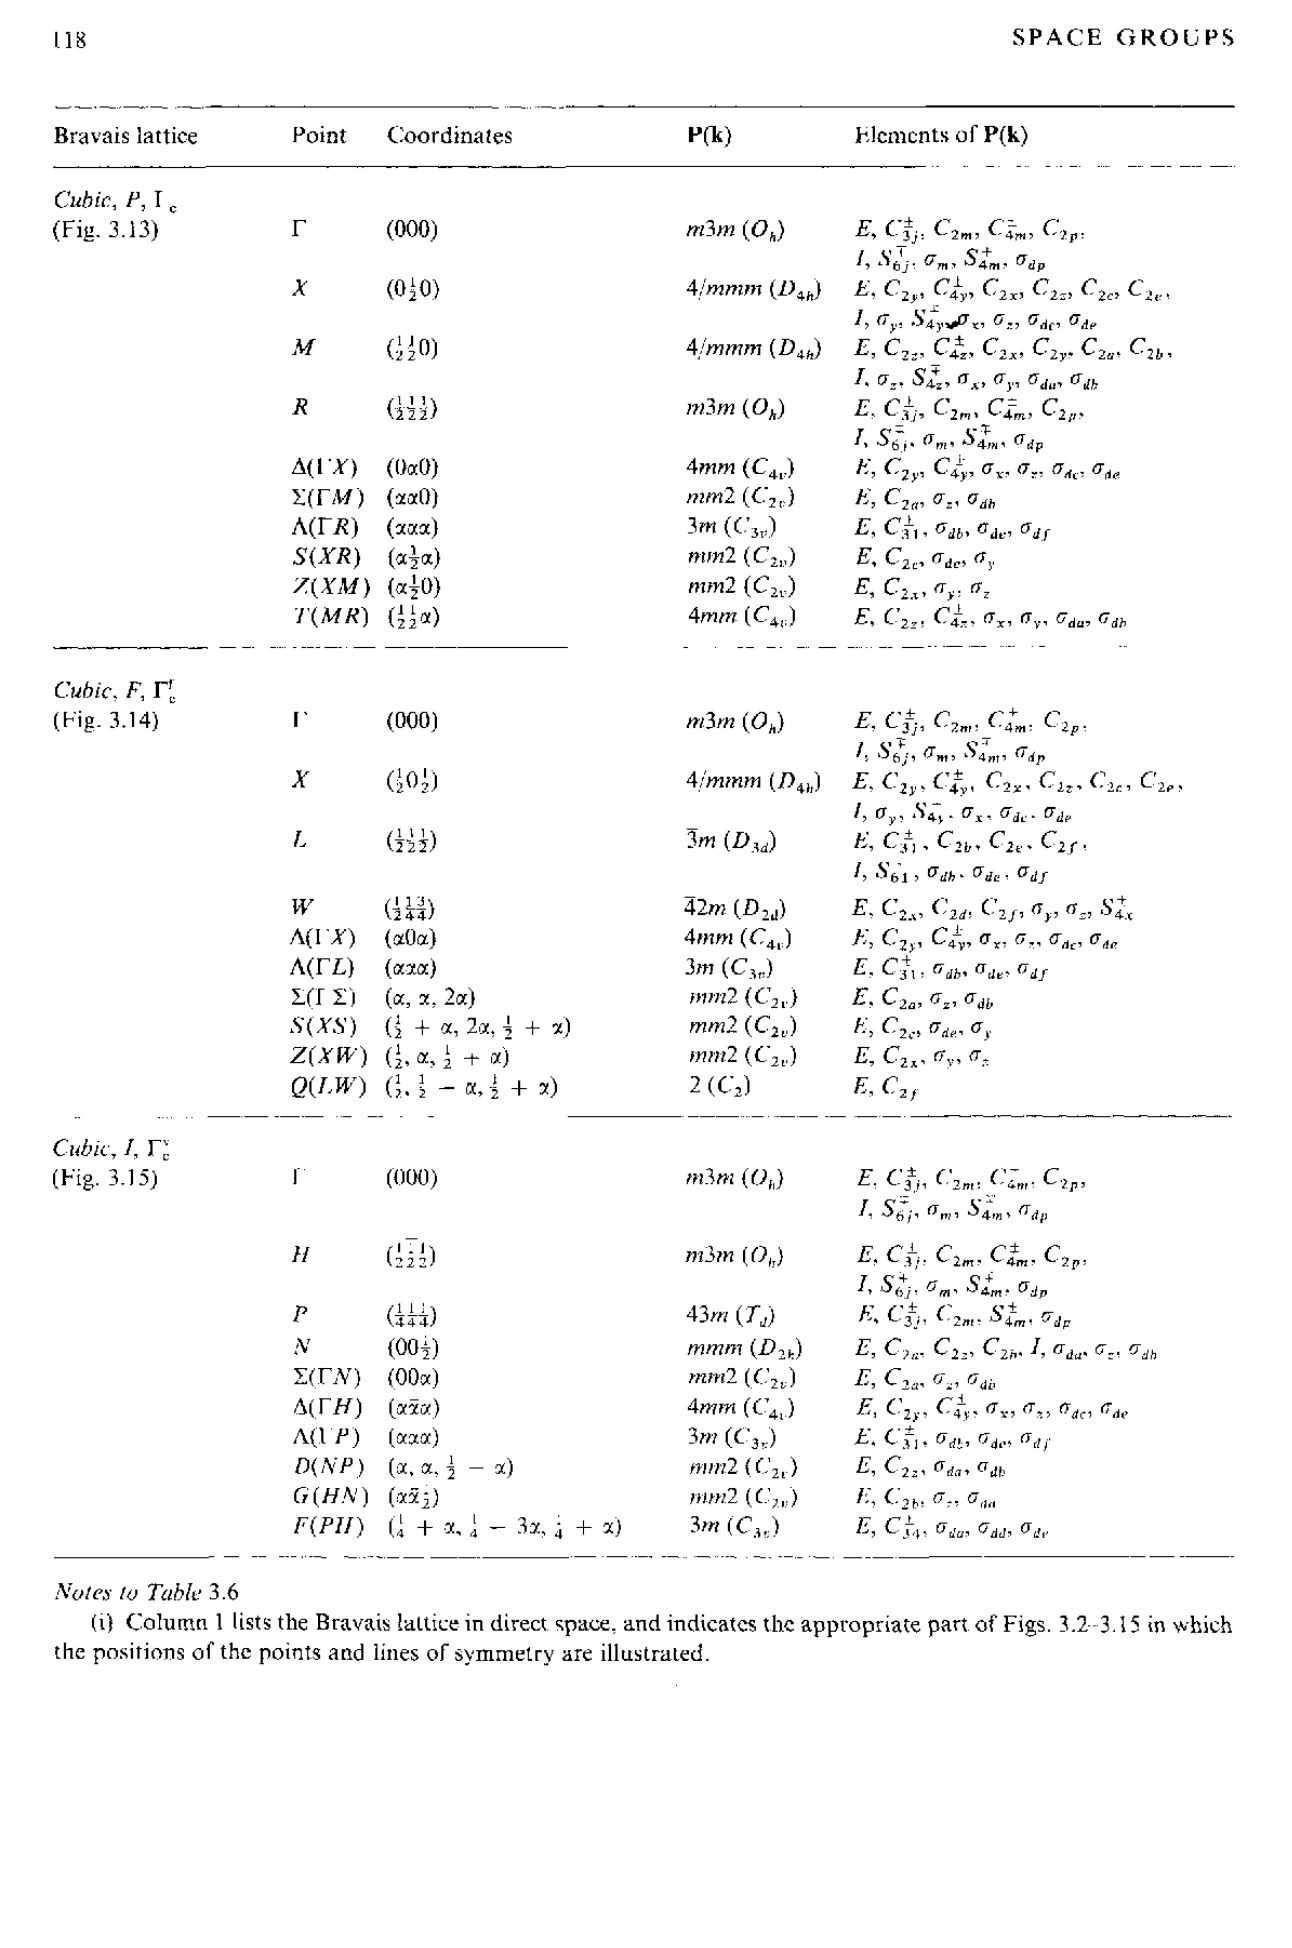
\includegraphics[width=0.92\textwidth]{c3_t36_p6.png}
\caption*{\textbf{表 3.6}（第 6 页，立方 $P$、$F$、$I$；页末起为表的注）。}
\end{figure}
\begin{figure}[H]
\centering
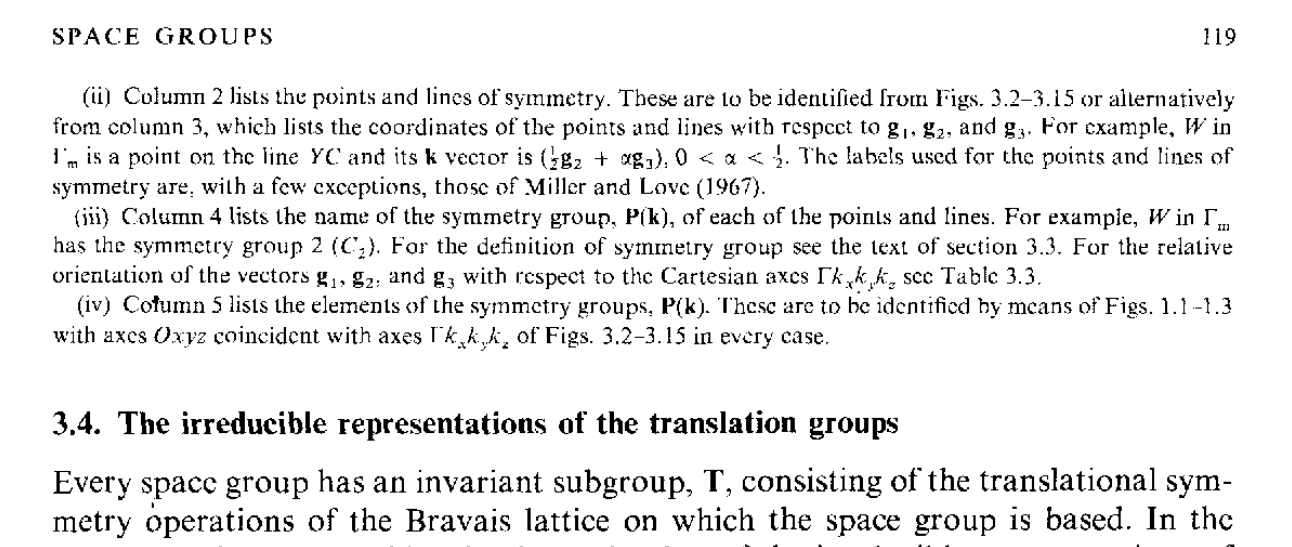
\includegraphics[width=0.92\textwidth]{c3_t36_p7.png}
\caption*{\textbf{表 3.6}（注 (ii)--(iv)，原书扫描占位）。}
\end{figure}

表 3.6 的注（译文）：

\noindent（i）第 1 列列出正空间的布拉维格子，并指出图 3.2--3.15 中展示各对称点和对称线位置的相应部分。

\noindent（ii）第 2 列列出对称点和对称线。它们既可从图 3.2--3.15 辨认，也可从第 3 列辨认；第 3 列列出各点和线相对于 $\mathbf{g}_{1}$、$\mathbf{g}_{2}$、$\mathbf{g}_{3}$ 的坐标。例如 $\Gamma_{m}$ 中的 $W$ 是线 $YC$ 上的一个点，其 $\mathbf{k}$ 矢量为 $\frac{1}{2}\mathbf{g}_{2}+\alpha\mathbf{g}_{3}$（$0<\alpha<\frac{1}{2}$）。对称点和对称线所用的标记，除少数例外，都是 Miller and Love（1967）的记号。

\noindent（iii）第 4 列列出各点和线的对称群 $\mathbf{P}(\mathbf{k})$ 的名称。例如 $\Gamma_{m}$ 中的 $W$ 具有对称群 $2\ (C_{2})$。对称群的定义见 3.3 节正文。矢量 $\mathbf{g}_{1}$、$\mathbf{g}_{2}$、$\mathbf{g}_{3}$ 相对于笛卡尔轴 $\Gamma k_{x}k_{y}k_{z}$ 的取向见表 3.3。

\noindent（iv）第 5 列列出对称群 $\mathbf{P}(\mathbf{k})$ 的元素。这些元素可借助图 1.1--1.3 来辨认，此时在所有情形下都取 $Oxyz$ 轴与图 3.2--3.15 的 $\Gamma k_{x}k_{y}k_{z}$ 轴重合。

\noindent（关于表中 $\Gamma_{rh}$ 的 $F$ 点的脚注：为了把 $F$ 保持在所选的基本域内，不得不让 (b) 中 $F$ 的 $\mathbf{P}(\mathbf{k})$ 元素与 (a) 中 $F$ 的不同，尽管这两个点显然是互相关联的。若允许 $F$ 位于所选基本域之外（即位于图 3.11(b) 的 $F'$ 处），本可使二者一致，但我们不拟这样做。）

% 3.4 平移群的不可约表示
\section{平移群的不可约表示}

每个空间群都有一个不变子群 $\mathbf{T}$，它由空间群所依托的布拉维格子的平移对称操作构成。本节考虑如何确定布拉维格子的平移对称操作群的不可约表示。

$\mathbf{T}$ 由元素 $\{E \mid n_{1}\mathbf{t}_{1} + n_{2}\mathbf{t}_{2} + n_{3}\mathbf{t}_{3}\}$ 构成，其中 $n_{i}$ 是满足 $0 \leqslant n_{i} < N_{i}$（$i = 1, 2$ 或 3）的整数，并且施加 Born--von Kármán 循环边界条件（Born and von Kármán 1913\textit{a}, \textit{b}）。由于乘法规则形如 $\{E \mid \mathbf{t}\}\{E \mid \mathbf{s}\} = \{E \mid \mathbf{t} + \mathbf{s}\}$，又由于式 (3.1.1) 所施加的周期性，$\mathbf{T}$ 是三个阶分别为 $N_{1}$、$N_{2}$、$N_{3}$ 的循环群的外直积，于是用明显的记号可以写 $\mathbf{T} = \mathbf{T}_{1} \otimes \mathbf{T}_{2} \otimes \mathbf{T}_{3}$。循环群的表示是众所周知的。例如，$\mathbf{T}_{1}$ 的表示 $\Delta$ 共有 $N_{1}$ 个，每一个用整数 $p_{1}$（$0 \leqslant p_{1} < N_{1}$）标记，使得
\begin{equation*}
\Delta^{p_{1}}(\{E \mid n_{1}\mathbf{t}_{1}\}) = \exp(-2\pi\mathrm{i}\, n_{1}p_{1}/N_{1}).
\tag{3.4.1}
\end{equation*}
由直积群上的定理 (1.3.16)，现在可以容易地导出 $\mathbf{T}$ 的表示。它们都是一维的，共 $N_{1}N_{2}N_{3}$ 个。每个表示用三个整数 $p_{1}$、$p_{2}$、$p_{3}$（$0 \leqslant p_{i} < N_{i}$）标记。若写 $k_{i} = p_{i}/N_{i}$，则可取 $\mathbf{k} = (k_{1}, k_{2}, k_{3})$ 为倒空间中的一个矢量，即
\begin{equation*}
\mathbf{k} = k_{1}\mathbf{g}_{1} + k_{2}\mathbf{g}_{2} + k_{3}\mathbf{g}_{3}.
\tag{3.4.2}
\end{equation*}
于是 $\mathbf{k}$ 可以拿来作为 $\mathbf{T}$ 的表示的标记，这些表示就是
\begin{equation*}
\Delta^{\mathbf{k}}\left[\{E \mid n_{1}\mathbf{t}_{1} + n_{2}\mathbf{t}_{2} + n_{3}\mathbf{t}_{3}\}\right] = \exp\left\{-\mathrm{i}\,\mathbf{k} \cdot (n_{1}\mathbf{t}_{1} + n_{2}\mathbf{t}_{2} + n_{3}\mathbf{t}_{3})\right\}.
\tag{3.4.3}
\end{equation*}
现在我们可以看出，为什么在定义中把相差一个倒格子矢量的两个 $\mathbf{k}$ 矢量称为等价。因为若 $\mathbf{k}' = \mathbf{k} + \mathbf{g}$，则由于 $\exp(-\mathrm{i}\,\mathbf{g} \cdot \mathbf{t}) = 1$，
\begin{equation*}
\Delta^{\mathbf{k}'}(\mathbf{t}) = \exp\left\{-\mathrm{i}(\mathbf{k} + \mathbf{g}) \cdot \mathbf{t}\right\} = \Delta^{\mathbf{k}}(\mathbf{t}).
\tag{3.4.4}
\end{equation*}
因此，可以取任意 $N_{1}N_{2}N_{3}$ 个互不等价的 $\mathbf{k}$ 矢量作为 $\mathbf{k}$ 的允许值。上面定义的那一组就是这样一组矢量，它们的终点落在倒空间初基晶胞的内部或表面上（除原点的移动之外）；对三斜和单斜布拉维格子，我们正是用这个初基晶胞来定义布里渊区的（见定义 3.2.2）。对所有其他布拉维格子，可以取终点落在倒空间 Wigner--Seitz 晶胞内部或表面上的那一组矢量作为 $N_{1}N_{2}N_{3}$ 个非等价的 $\mathbf{k}$ 矢量（见定义 3.2.1）。这样，在任何情形下我们都可以把 $\mathbf{T}$ 的表示看作由布里渊区的点 $\mathbf{k}$ 所定义的。

有一个关于允许的 $\mathbf{k}$ 矢量密度的公式会很有用。在体积 $8\pi^{3}/V$（$V$ 是晶体晶胞的体积）中共有 $N_{1}N_{2}N_{3}$ 个 $\mathbf{k}$ 矢量。因此密度 $n(\mathbf{k})$ 为 $N_{1}N_{2}N_{3}V/8\pi^{3} = W/8\pi^{3}$，其中 $W$ 是晶体的体积。于是
\begin{equation*}
n(\mathbf{k}) = \frac{W}{8\pi^{3}}.
\tag{3.4.5}
\end{equation*}
这意味着，在无穷晶体的极限下，$\mathbf{k}$ 的取值变得任意接近，从而稠密地填满整个布里渊区。

$\Delta^{\mathbf{k}}$ 的基函数可以取 $\exp(\mathrm{i}\mathbf{k} \cdot \mathbf{r})$，因为由例 1.5.3，
\begin{equation*}
\begin{aligned}
\{E \mid \mathbf{t}\}\exp(\mathrm{i}\mathbf{k} \cdot \mathbf{r}) &= \exp\left\{\mathrm{i}\mathbf{k} \cdot (\mathbf{r} - \mathbf{t})\right\} \\
&= \exp(-\mathrm{i}\mathbf{k} \cdot \mathbf{t})\exp(\mathrm{i}\mathbf{k} \cdot \mathbf{r}) = \Delta^{\mathbf{k}}\{E \mid \mathbf{t}\}\exp(\mathrm{i}\mathbf{k} \cdot \mathbf{r}).
\end{aligned}
\tag{3.4.6}
\end{equation*}
代替 $\exp(\mathrm{i}\mathbf{k} \cdot \mathbf{r})$，我们可以使用任何形如
\begin{equation*}
\Psi_{\mathbf{k}}(\mathbf{r}) = \exp(\mathrm{i}\mathbf{k} \cdot \mathbf{r})\,u_{\mathbf{k}}(\mathbf{r})
\tag{3.4.7}
\end{equation*}
的函数，其中
\begin{equation*}
u_{\mathbf{k}}(\mathbf{r}) = u_{\mathbf{k}}(\mathbf{r} + \mathbf{t})
\tag{3.4.8}
\end{equation*}
对一切 $\mathbf{t}$ 成立。平移群 $\mathbf{T}$ 的基函数具有式 (3.4.7) 与 (3.4.8) 所定义的形式，这一结论通常称为 Bloch 定理。

\noindent\textbf{定理 3.4.1}\quad （Bloch 定理）（Bloch 1928）\ 在由 $\mathbf{T}$ 定义其周期性的周期性势场 $V(\mathbf{r})$ 中运动的粒子或准粒子的波函数可以写成
\begin{equation*}
\Psi_{\mathbf{k}}(\mathbf{r}) = \exp(\mathrm{i}\mathbf{k} \cdot \mathbf{r})\,u_{\mathbf{k}}(\mathbf{r})
\tag{3.4.7}
\end{equation*}
的形式，其中 $u_{\mathbf{k}}(\mathbf{r})$ 与 $V(\mathbf{r})$ 具有相同的周期性，而 $\mathbf{k}$ 由式 (3.4.2) 确定。\footnote{中译者注：原书在定理 3.4.1 中重复使用了编号 (3.4.7)，照录。}

然而必须强调，Bloch 函数 $\Psi_{\mathbf{k}}(\mathbf{r})$ 上的标记 $\mathbf{k}$，正如表示本身一样，只是在等价的意义下确定的，可以增减倒格矢 $\mathbf{g}$ 而改变。这是因为 $\exp(\mathrm{i}\mathbf{g} \cdot \mathbf{r})$ 满足式 (3.4.8)，所以任何这样的因子都可以吸收进 Bloch 函数的 $u_{\mathbf{k}}(\mathbf{r})$ 部分。如果所考虑的晶体置于均匀的外电场或外磁场中，理论就需要作一些修改（例如见 Ashby and Miller (1965)）。

% 3.5 230 个三维空间群的分类
\section{三维空间群 230 种的分类}

到目前为止，我们在本章中讨论的都是空间群的平移对称性。空间群 $\mathbf{G}$ 有一个三维的纯平移子群 $\mathbf{T}$，它确定布拉维格子。布拉维格子具有 $\mathbf{T}$ 的对称性；此外它还在点群 $\mathbf{P}$ 的操作下不变。事实上，若 $\mathbf{F}$ 是布拉维格子的全对称群，则 $\mathbf{F} = \mathbf{T} \wedge \mathbf{P}$，即 $\mathbf{T}$ 与 $\mathbf{P}$ 的半直积（半直积的含义见定义 (1.2.17)）。$\mathbf{P}$ 确定 $\mathbf{G}$ 的晶系。$\mathbf{F}$ 本身是一个空间群。若 $\mathbf{G}$ 是点式的，则 $\mathbf{G}$ 要么与 $\mathbf{F}$ 重合，要么是 $\mathbf{F}$ 的子群；这就给出 73 个空间群，见 1.5 节。显然此时 $\mathbf{G} = \mathbf{T} \wedge \mathbf{Q}$，其中 $\mathbf{Q}$ 是 $\mathbf{P}$ 所属晶系中的一个点群。$\mathbf{Q}$ 确定该晶体的点群，而空间群为 $\mathbf{G}$ 的晶体就属于这个点群。

其余 157 个非点式空间群可以这样得到：把 $\mathbf{Q}$ 的一部分元素换成螺旋轴转动或滑移面反射。此时 $\mathbf{Q}$ 不再是群，也就不能再写 $\mathbf{G} = \mathbf{T} \wedge \mathbf{Q}$；这是因为，若集合 $\mathbf{Q}$ 的元素能够取成一组构成群，则它将同构于某个点群，从而 $\mathbf{G}$ 又将同构于某个点式空间群。

现在考虑必须对 $\mathbf{Q}$ 的元素 $\{R \mid \mathbf{v}\}$ 施加哪些限制，才能使 $\mathbf{G}$ 成为一个空间群。以下讨论对点式空间群显然成立，因此可以视为完整的刻画。首先 $\mathbf{G}$ 必须是群。于是，若 $\{R \mid \mathbf{v}\}$ 是 $\mathbf{G}$ 的元素，则其逆 $\{R^{-1} \mid -R^{-1}\mathbf{v}\}$ 也必须是 $\mathbf{G}$ 的元素（见式 (1.5.3)）。因此，若 $\{R \mid \mathbf{w}\}$ 也在 $\mathbf{G}$ 中，则
\begin{equation*}
\{R^{-1} \mid -R^{-1}\mathbf{v}\}\{R \mid \mathbf{w}\} = \{E \mid R^{-1}\mathbf{w} - R^{-1}\mathbf{v}\}
\tag{3.5.1}
\end{equation*}
也是 $\mathbf{G}$ 的元素。事实上它必属于平移子群 $\mathbf{T}$，因为其转动部分是恒等元。其次，$\mathbf{G}$ 有一个属于某一晶系的布拉维格子，该晶系的全对称点群 $\mathbf{P}$ 必须包含操作 $R$。于是，如式 (3.5.1) 所蕴含的，若 $R^{-1}(\mathbf{w} - \mathbf{v})$ 是 $\mathbf{F}$ 的一个平移，则 $(\mathbf{w} - \mathbf{v})$ 也是。这意味着与任一点群操作相联系的平移部分相差的只能是 $\mathbf{T}$ 的元素。因此可以用 $\mathbf{T}$ 的左陪集代表把 $\mathbf{G}$ 写成（见定义 1.2.9）
\begin{equation*}
\mathbf{G} = \{R_{1} \mid \mathbf{v}_{1}\}\mathbf{T} + \{R_{2} \mid \mathbf{v}_{2}\}\mathbf{T} + \dots + \{R_{h} \mid \mathbf{v}_{h}\}\mathbf{T},
\tag{3.5.2}
\end{equation*}
并且可以选择 $R_{1} = E$，而 $\mathbf{v}_{i}$ 取为与 $R_{i}$（$i = 1$ 至 $h$）相联系的、模长尽可能小的矢量。于是对点式空间群所有的 $\mathbf{v}_{i}$ 都是零，而对非点式空间群则必须有一个或多个 $\mathbf{v}_{i}$ 非零。$\mathbf{Q}$ 由陪集代表 $\{R_{i} \mid \mathbf{v}_{i}\}$ 组成。$h$ 个元素 $R_{1}, R_{2}, \dots, R_{h}$ 构成一个点群 $\mathbf{F}$，即 $\mathbf{G}$ 的同形点群（见 1.5 节）。$\mathbf{F}$ 是 $\mathbf{P}$ 的子群。对点式空间群，$\mathbf{F}$ 与 $\mathbf{Q}$ 重合。$h$ 称为 $\mathbf{G}$ 的\textit{宏观阶}（macroscopic order），它是 $\mathbf{T}$ 在 $\mathbf{G}$ 中的指数。

在上述描述中，非零矢量 $\mathbf{v}$ 并非任意的，因为要满足 $\mathbf{G}$ 的群的要求。例如，若 $R$ 的阶为 $n$，则 $\{R \mid \mathbf{v}\}^{n}$ 必须属于 $\mathbf{T}$，即 $(\mathbf{v} + R\mathbf{v} + \dots + R^{n-1}\mathbf{v})$ 必须是一个平移。这一要求以及其他类似要求把非点式空间群的数目限制为 157 个，总计 230 个空间群。

\noindent\textbf{定理 3.5.1}\quad $\mathbf{T}$ 是 $\mathbf{G}$ 的不变子群。因为若 $\{R \mid \mathbf{v}\}$ 是 $\mathbf{G}$ 的元素，$\{E \mid \mathbf{t}\}$ 是 $\mathbf{T}$ 的元素，则
\begin{equation*}
\{R \mid \mathbf{v}\}\{E \mid \mathbf{t}\}\{R \mid \mathbf{v}\}^{-1} = \{R \mid \mathbf{v} + R\mathbf{t}\}\{R^{-1} \mid -R^{-1}\mathbf{v}\} = \{E \mid R\mathbf{t}\}
\tag{3.5.3}
\end{equation*}
属于 $\mathbf{T}$，因为 $R\mathbf{t}$ 是 $\mathbf{T}$ 的一个平移。

每个空间群诸元素的 Seitz 空间群符号已由许多作者给出（Faddeyev 1964, Koptsik 1966, Kovalev 1965, Lyubarskii 1960, Miller and Love 1967），也可以利用《X 射线晶体学国际表》（Henry and Lonsdale 1965）写出来。在该表的第 4.3 节中，对每个空间群给出了晶胞中等价位置的一组坐标；对每个非立方空间群还给出了图示其对称元素的图。利用这些表不仅能够得到以 Seitz 符号 $\{R_{i} \mid \mathbf{v}_{i}\}$ 表示的空间群元素，还能对这些对称操作作出几何解释；例如对一根螺旋转动轴，可以确定轴的方向以及转动的大小和沿轴平移的大小（Wondratschek and Neubüser 1967）。我们将通过例子说明《国际表》中等价位置的这两种用法。

我们以基于正交初基布拉维格子的空间群 $Pmmn$（$D_{2h}^{13}$）为例，说明如何利用《国际表》给出的等价位置确定相应的 Seitz 空间群符号。等价位置既对晶胞中完全一般的点给出，也对位于各种对称元素上的点给出。图 3.17 复制了《国际表》第一卷第 4.3 节中与 $Pmmn$（$D_{2h}^{13}$）有关的两页。在图 3.17(a) 中，第一组等价位置对应于晶胞中的一般点 $(x, y, z)$；其余各组等价位置对应于位于某个对称轴或对称面上的点 $(x, y, z)$，这些与我们无关。从点 $\mathbf{r}_{1}\,(=(x, y, z))$ 出发，施加由 $\{R_{1} \mid \mathbf{v}_{1}\}$ 表示的空间群操作，由式 (1.5.2) 得
\begin{equation*}
\mathbf{r}_{1}' = R_{1}\mathbf{r}_{1} + \mathbf{v}_{1}
\tag{3.5.4}
\end{equation*}
所得的矢量 $\mathbf{r}_{1}'$ 为
\begin{center}
\begin{tabular}{cccc}
$x, y, z$;\quad & $\bar{x}, \bar{y}, z$;\quad & $\bar{x}, y, z$;\quad & $x, \bar{y}, z$;\quad \\[0.5ex]
$\frac{1}{2}-x, \frac{1}{2}-y, \bar{z}$;\quad & $\frac{1}{2}-x, \frac{1}{2}+y, \bar{z}$;\quad & $\frac{1}{2}+x, \frac{1}{2}+y, \bar{z}$;\quad & $\frac{1}{2}+x, \frac{1}{2}-y, \bar{z}$.
\end{tabular}
\end{center}
这些分数是指《国际表》中对每个空间群（立方空间群除外）所画的惯用晶胞在 $x$、$y$、$z$ 方向的棱长的分数。利用表 1.4 可以对这八个 $\mathbf{r}_{1}'$ 逐一辨认出 $R_{1}$：
\begin{center}
\begin{tabular}{cccccccc}
$xyz$;\quad & $\bar{x}\bar{y}z$;\quad & $\bar{x}yz$;\quad & $x\bar{y}z$;\quad & $\bar{x}\bar{y}\bar{z}$;\quad & $\bar{x}y\bar{z}$;\quad & $xy\bar{z}$;\quad & $x\bar{y}\bar{z}$;\\
$E$;\quad & $C_{2z}$;\quad & $\sigma_{x}$;\quad & $\sigma_{y}$;\quad & $I$;\quad & $C_{2y}$;\quad & $\sigma_{z}$;\quad & $C_{2x}$
\end{tabular}
\end{center}
这就给出了空间群符号中的转动部分。与其中前四个相联系的平移矢量 $\mathbf{v}_{1}$ 显然为零。由于对正交初基布拉维格子有 $\mathbf{t}_{1} = (0, -b, 0)$、$\mathbf{t}_{2} = (a, 0, 0)$（见表 3.1），与后四个符号相联系的平移矢量是 $-\frac{1}{2}\mathbf{t}_{1} + \frac{1}{2}\mathbf{t}_{2}$。可以在平移矢量 $\mathbf{v}_{1}$ 上加上 $\mathbf{t}_{1}$、$\mathbf{t}_{2}$ 或 $\mathbf{t}_{3}$ 的整数倍，因此我们取 $\mathbf{v}_{1} = +\frac{1}{2}\mathbf{t}_{1} + \frac{1}{2}\mathbf{t}_{2}$，于是空间群 $Pmmn$（$D_{2h}^{13}$）的元素为
\begin{center}
$\{E \mid 000\}$，$\{C_{2z} \mid 000\}$，$\{\sigma_{x} \mid 000\}$，$\{\sigma_{y} \mid 000\}$，\\[0.5ex]
$\{I \mid \frac{1}{2}\frac{1}{2}0\}$，$\{C_{2y} \mid \frac{1}{2}\frac{1}{2}0\}$，$\{\sigma_{z} \mid \frac{1}{2}\frac{1}{2}0\}$，以及 $\{C_{2x} \mid \frac{1}{2}\frac{1}{2}0\}$。
\end{center}
不必把所有这些元素都列出来：在表 3.7 中我们只列出了每个空间群的生成元。在 $Pmmn$（$D_{2h}^{13}$）名下可以看到，选取的生成元是 $\{C_{2x} \mid \frac{1}{2}\frac{1}{2}0\}$、$\{C_{2y} \mid \frac{1}{2}\frac{1}{2}0\}$ 和 $\{I \mid \frac{1}{2}\frac{1}{2}0\}$。

\begin{figure}[H]
\centering
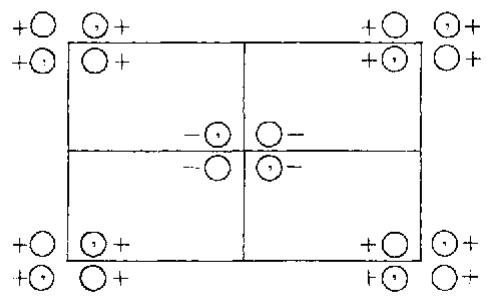
\includegraphics[width=0.72\textwidth]{fig3_17a_mu.jpg}
\caption*{\textbf{图 3.17(a)}\ 《国际表》（Henry and Lonsdale 1965）书影：$Pmmn$（$D_{2h}^{13}$）的第一种定向（原点在 $mmn$）。}
\end{figure}
\begin{figure}[H]
\centering
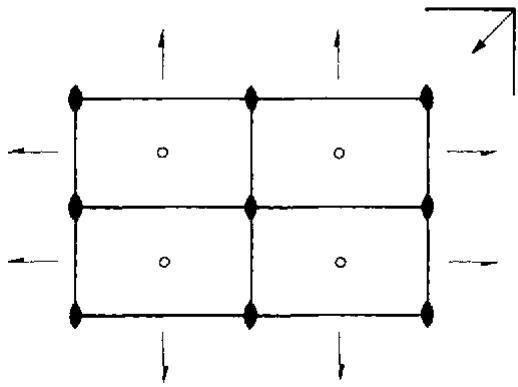
\includegraphics[width=0.72\textwidth]{fig3_17b_mu.jpg}
\caption*{\textbf{图 3.17(b)}\ 同上，第二种定向（原点在 $\bar{1}$）。}
\end{figure}

重要的是要弄清：若把描述晶体所用的坐标系原点移到晶胞中另一点，给定的 Seitz 空间群符号 $\{R_{1} \mid \mathbf{v}_{1}\}$ 的形式会受到什么影响。设 $\mathbf{r}_{1}$ 与 $\mathbf{r}_{1}'$ 是某个点在施加一个主动空间群对称操作前、后的位置；在第一组坐标轴 $O_{1}x_{1}y_{1}z_{1}$ 中该操作记为 $\{R_{1} \mid \mathbf{v}_{1}\}$。现在另取一组坐标轴 $O_{2}x_{2}y_{2}z_{2}$，其原点相对 $O_{1}x_{1}y_{1}z_{1}$ 的原点移动了矢量 $+\mathbf{t}_{0}$ 而轴不转动，见图 3.18。由该图可见
\begin{equation*}
\mathbf{r}_{1} = \mathbf{t}_{0} + \mathbf{r}_{2}
\tag{3.5.5}
\end{equation*}
及
\begin{equation*}
\mathbf{r}_{1}' = \mathbf{t}_{0} + \mathbf{r}_{2}',
\tag{3.5.6}
\end{equation*}
又由在 $O_{1}x_{1}y_{1}z_{1}$ 中使用的空间群符号 $\{R_{1} \mid \mathbf{v}_{1}\}$ 的定义，
\begin{equation*}
\mathbf{r}_{1}' = R_{1}\mathbf{r}_{1} + \mathbf{v}_{1}.
\tag{3.5.4}
\end{equation*}
若这一空间群操作在坐标系 $O_{2}x_{2}y_{2}z_{2}$ 中记为 $\{R_{2} \mid \mathbf{v}_{2}\}$，则 $\mathbf{r}_{2}'$ 与 $\mathbf{r}_{2}$ 满足
\begin{equation*}
\mathbf{r}_{2}' = R_{2}\mathbf{r}_{2} + \mathbf{v}_{2}
\tag{3.5.7}
\end{equation*}
于是可以用这些方程把 $\{R_{2} \mid \mathbf{v}_{2}\}$ 用 $\{R_{1} \mid \mathbf{v}_{1}\}$ 表示出来。由式 (3.5.7)，
\begin{align*}
R_{2}\mathbf{r}_{2} + \mathbf{v}_{2} &= \mathbf{r}_{2}' = \mathbf{r}_{1}' - \mathbf{t}_{0} \quad\text{（由 (3.5.6)）}\\
&= R_{1}\mathbf{r}_{1} + \mathbf{v}_{1} - \mathbf{t}_{0} \quad\text{（由 (3.5.4)）}\\
&= R_{1}(\mathbf{t}_{0} + \mathbf{r}_{2}) + \mathbf{v}_{1} - \mathbf{t}_{0} \quad\text{（由 (3.5.5)）}\\
&= R_{1}\mathbf{r}_{2} + \mathbf{v}_{1} + R_{1}\mathbf{t}_{0} - \mathbf{t}_{0},
\end{align*}
即
\begin{equation*}
R_{2}\mathbf{r}_{2} + \mathbf{v}_{2} = R_{1}\mathbf{r}_{2} + \mathbf{v}_{1} + R_{1}\mathbf{t}_{0} - \mathbf{t}_{0}.
\tag{3.5.8}
\end{equation*}
比较式 (3.5.8) 两边可见，把原点移动 $+\mathbf{t}_{0}$ 对空间群符号 $\{R_{1} \mid \mathbf{v}_{1}\}$ 的效果是产生 $\{R_{2} \mid \mathbf{v}_{2}\}$，其中
\begin{equation*}
R_{2} = R_{1}
\tag{3.5.9}
\end{equation*}
及
\begin{equation*}
\mathbf{v}_{2} = \mathbf{v}_{1} + R_{1}\mathbf{t}_{0} - \mathbf{t}_{0}.
\tag{3.5.10}
\end{equation*}
也就是说，移动原点 $+\mathbf{t}_{0}$ 对空间群符号 $\{R_{1} \mid \mathbf{v}_{1}\}$ 的效果是产生
\begin{equation*}
\{R_{2} \mid \mathbf{v}_{2}\} = \{R_{1} \mid \mathbf{v}_{1} + R_{1}\mathbf{t}_{0} - \mathbf{t}_{0}\}.
\tag{3.5.11}
\end{equation*}

\begin{figure}[H]
\centering
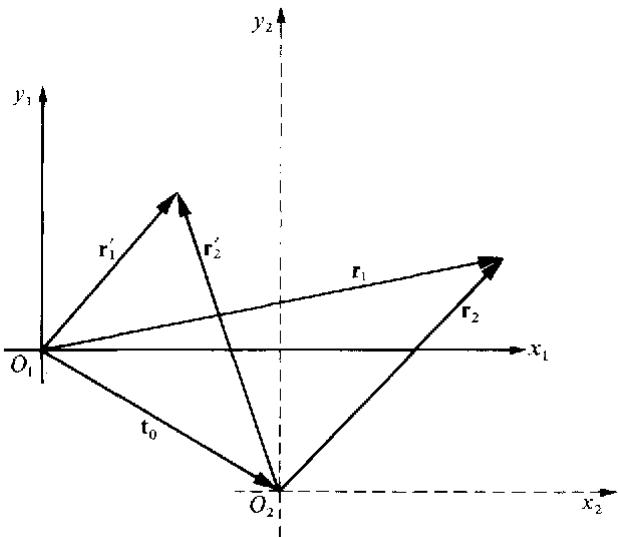
\includegraphics[width=0.55\textwidth]{fig3_18_mu.jpg}
\caption*{\textbf{图 3.18}\ 通过一个平移改变原点。}
\end{figure}

我们仍以空间群 $Pmmn$（$D_{2h}^{13}$）为例说明移动原点对空间群符号的影响。《国际表》对该空间群给出了两种不同的定向，见图 3.17。上面我们已用第一种定向（图 3.17(a)）写出了空间群元素。在第二种定向（图 3.17(b)）中，原点移动了（沿 $x$ 轴重复距离的 $-\frac{1}{4}$）加（沿 $y$ 轴重复距离的 $-\frac{1}{4}$），即由表 3.1，
\begin{equation*}
\mathbf{t}_{0} = \frac{1}{4}\mathbf{t}_{1} - \frac{1}{4}\mathbf{t}_{2}.
\tag{3.5.12}
\end{equation*}
于是利用式 (3.5.9) 与 (3.5.10)，可以把先前得到的空间群元素转换到第二组轴上。例如 $\{C_{2z} \mid 000\}$ 被 $\{R_{2} \mid \mathbf{v}_{2}\}$ 取代，其中由式 (3.5.9)，$R_{2} = C_{2z}$，而
\begin{align*}
\mathbf{v}_{2} &= \mathbf{v}_{1} + R_{1}\mathbf{t}_{0} - \mathbf{t}_{0}\\
&= \mathbf{0} + C_{2z}\left(\tfrac{1}{4}\mathbf{t}_{1} - \tfrac{1}{4}\mathbf{t}_{2}\right) - \left(\tfrac{1}{4}\mathbf{t}_{1} - \tfrac{1}{4}\mathbf{t}_{2}\right)\\
&= \left(-\tfrac{1}{4}\mathbf{t}_{1} + \tfrac{1}{4}\mathbf{t}_{2}\right) - \left(\tfrac{1}{4}\mathbf{t}_{1} - \tfrac{1}{4}\mathbf{t}_{2}\right)\quad\text{（由表 3.2）}\\
&= -\tfrac{1}{2}\mathbf{t}_{1} + \tfrac{1}{2}\mathbf{t}_{2},
\tag{3.5.13}
\end{align*}
故新坐标系中的元素为 $\{C_{2z} \mid \bar{\frac{1}{2}}\bar{\frac{1}{2}}0\}$，可以加上 $\mathbf{t}_{1}$ 得到以新原点为基准的空间群元素 $\{C_{2z} \mid \frac{1}{2}\frac{1}{2}0\}$。这与图 3.17(b) 所示的等价位置一致：$\{C_{2z} \mid \frac{1}{2}\frac{1}{2}0\}$ 作用在 $(x, y, z)$ 上产生 $(\frac{1}{2}-x, \frac{1}{2}-y, z)$，这正是图 3.17(b) 给出的八个一般等价位置之一。对同样的 $\mathbf{t}_{0} = \frac{1}{4}\mathbf{t}_{1} - \frac{1}{4}\mathbf{t}_{2}$ 反复使用式 (3.5.9) 与 (3.5.10)，得到以新原点为基准的空间群 $Pmmn$（$D_{2h}^{13}$）的全部元素：
\begin{center}
$\{E \mid 000\}$，$\{C_{2z} \mid \frac{1}{2}\frac{1}{2}0\}$，$\{\sigma_{x} \mid 0\frac{1}{2}0\}$，$\{\sigma_{y} \mid \frac{1}{2}00\}$，\\[0.5ex]
$\{I \mid 000\}$，$\{\sigma_{z} \mid \frac{1}{2}\frac{1}{2}0\}$，$\{C_{2x} \mid 0\frac{1}{2}0\}$，$\{C_{2y} \mid \frac{1}{2}00\}$。
\end{center}
在这个清单里，我们在某些情况下加上或减去了正交初基布拉维格子平移群的矢量，以简化空间群元素的形式。

230 个空间群中每一个的生成元都列于表 3.7。在前三列中我们用国际符号和 Schönflies 符号标识空间群，第 4 列给出足以确定空间群 $\mathbf{G}$ 全部元素的 Seitz 空间群符号，其中 $\{R \mid pqr\}$ 表示 $\{R \mid p\mathbf{t}_{1} + q\mathbf{t}_{2} + r\mathbf{t}_{3}\}$，$\mathbf{t}_{1}$、$\mathbf{t}_{2}$、$\mathbf{t}_{3}$ 按表 3.1 的定义。这些操作一如既往地用 1.5 节解释的 Seitz 记号表示（见式 (1.5.2) 与 (1.5.3)）。

\begin{figure}[H]
\centering
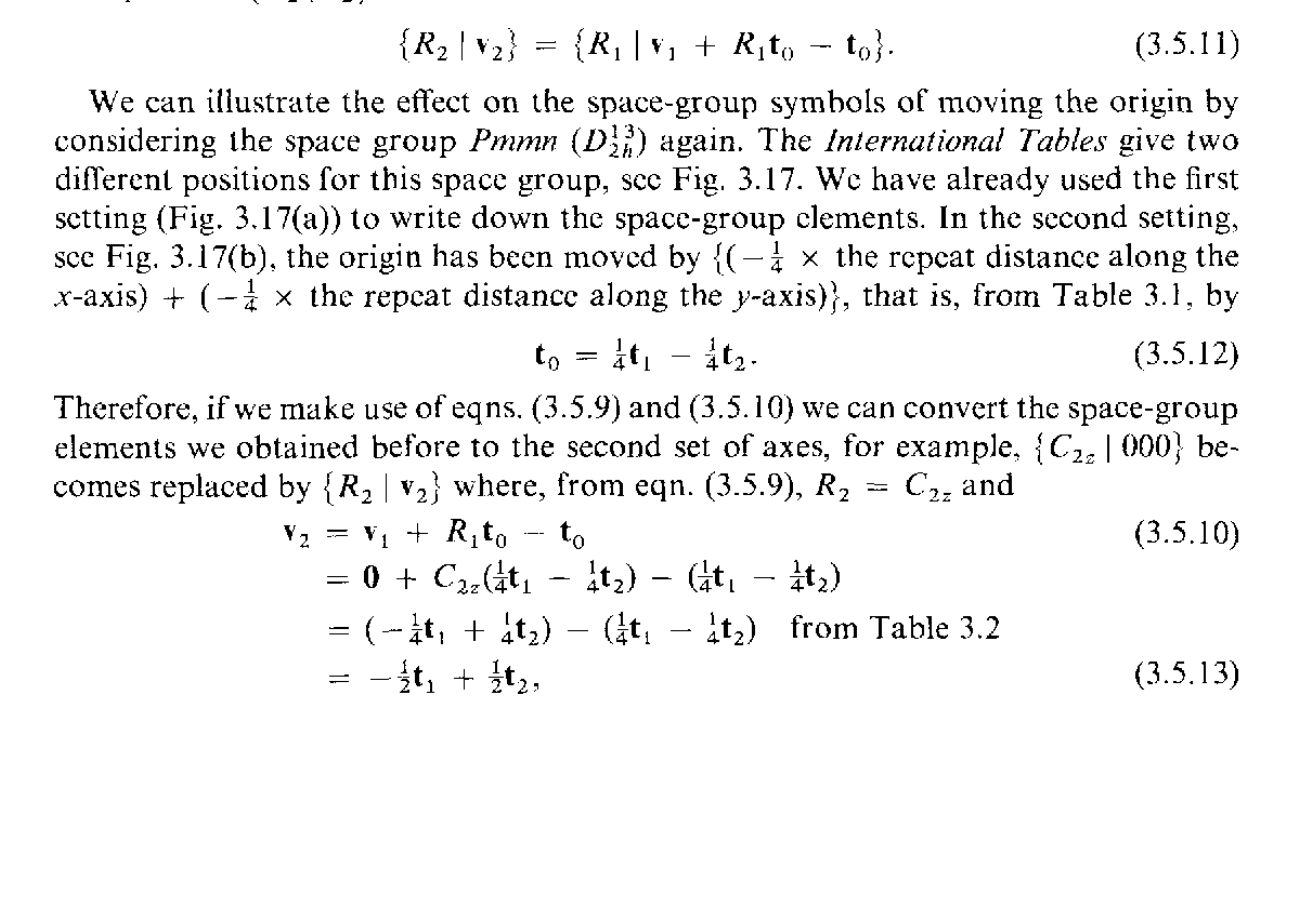
\includegraphics[width=0.92\textwidth]{c3_t37_p1.png}
\caption*{\textbf{表 3.7}\ 230 个空间群（原书第 126 页起扫描；第 1 页）。}
\end{figure}
\begin{figure}[H]
\centering
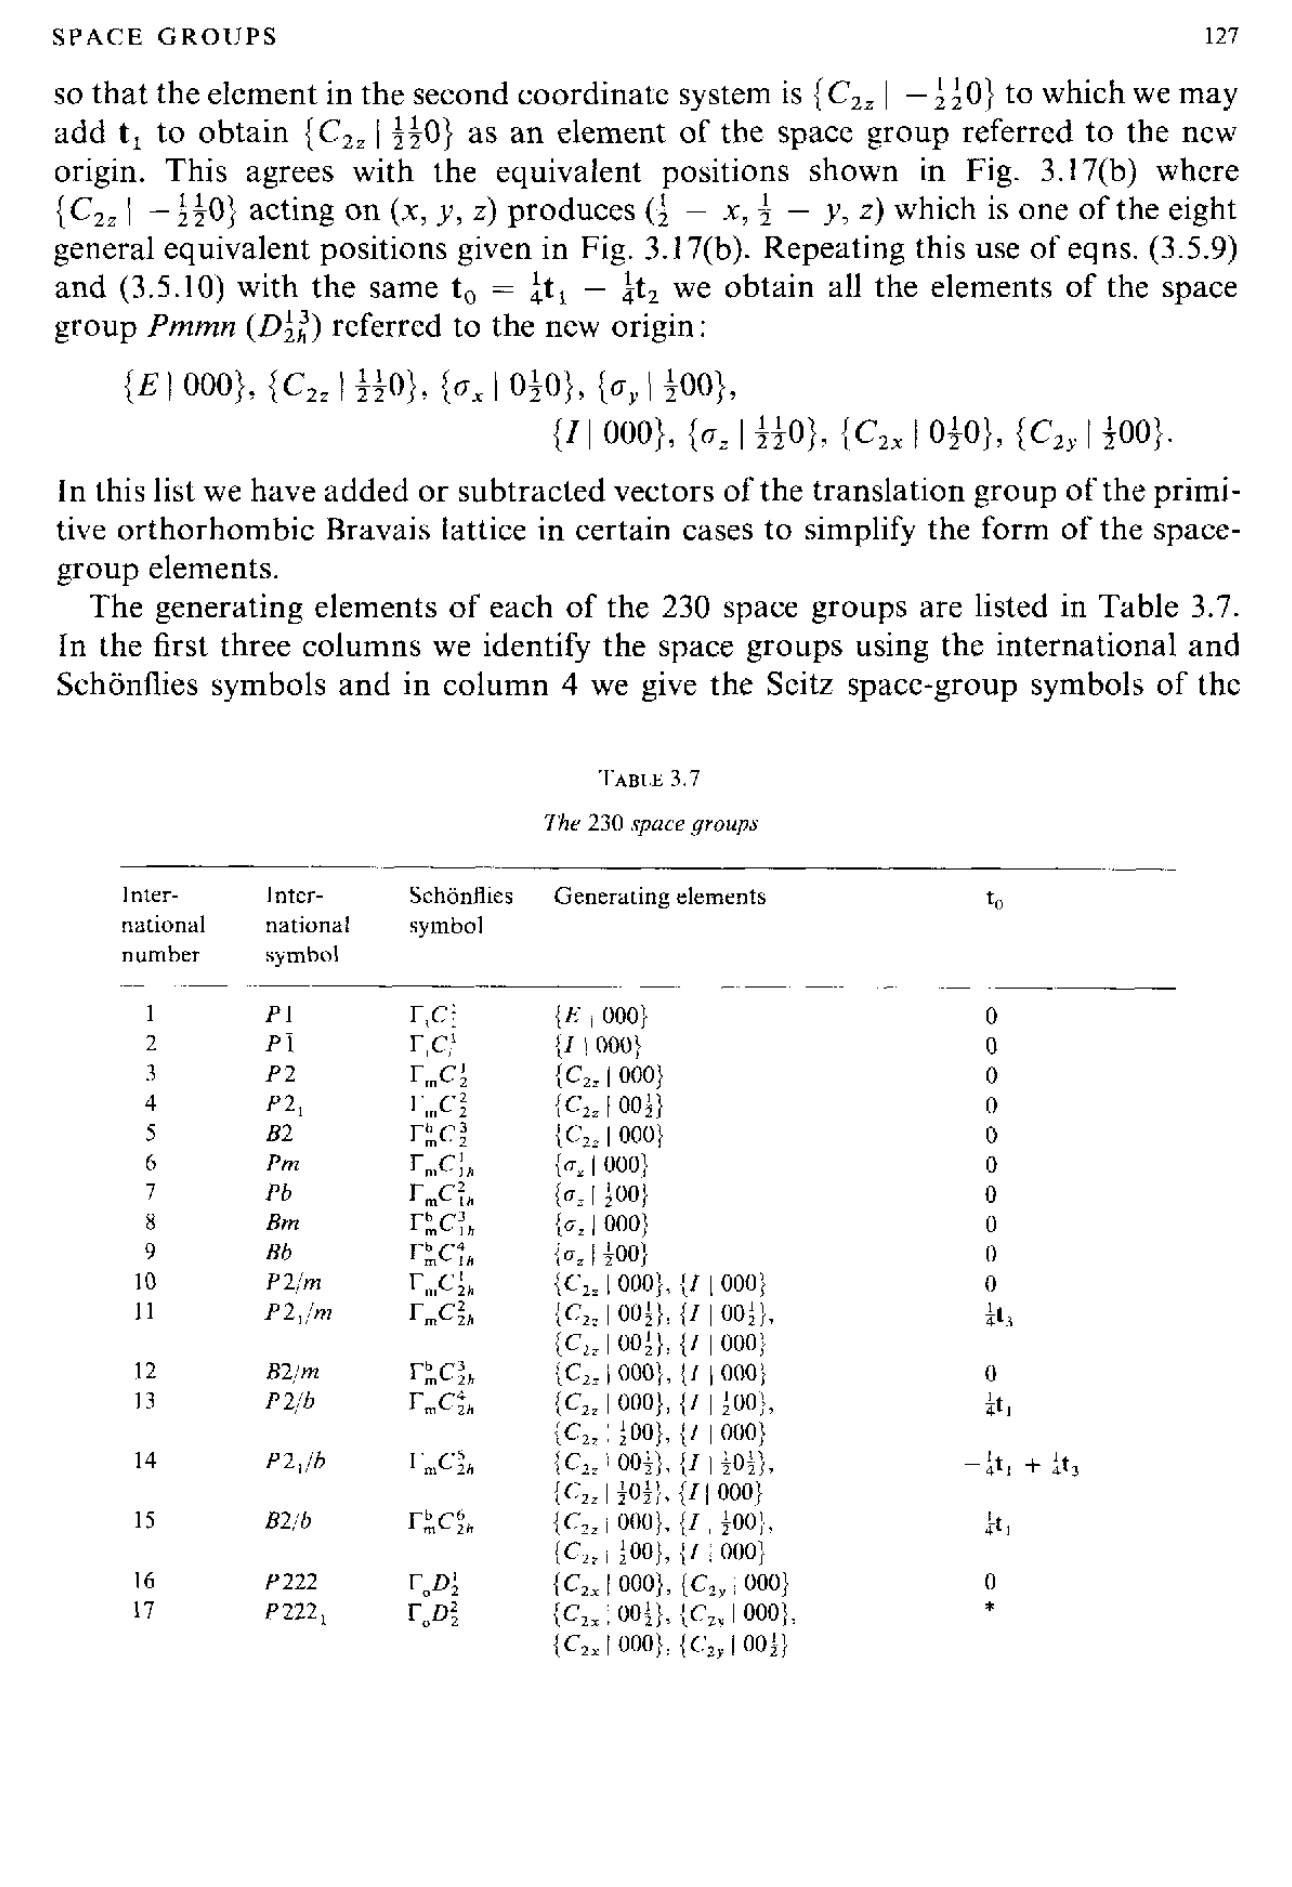
\includegraphics[width=0.92\textwidth]{c3_t37_p2.png}
\caption*{\textbf{表 3.7}（第 2 页）。}
\end{figure}
\begin{figure}[H]
\centering
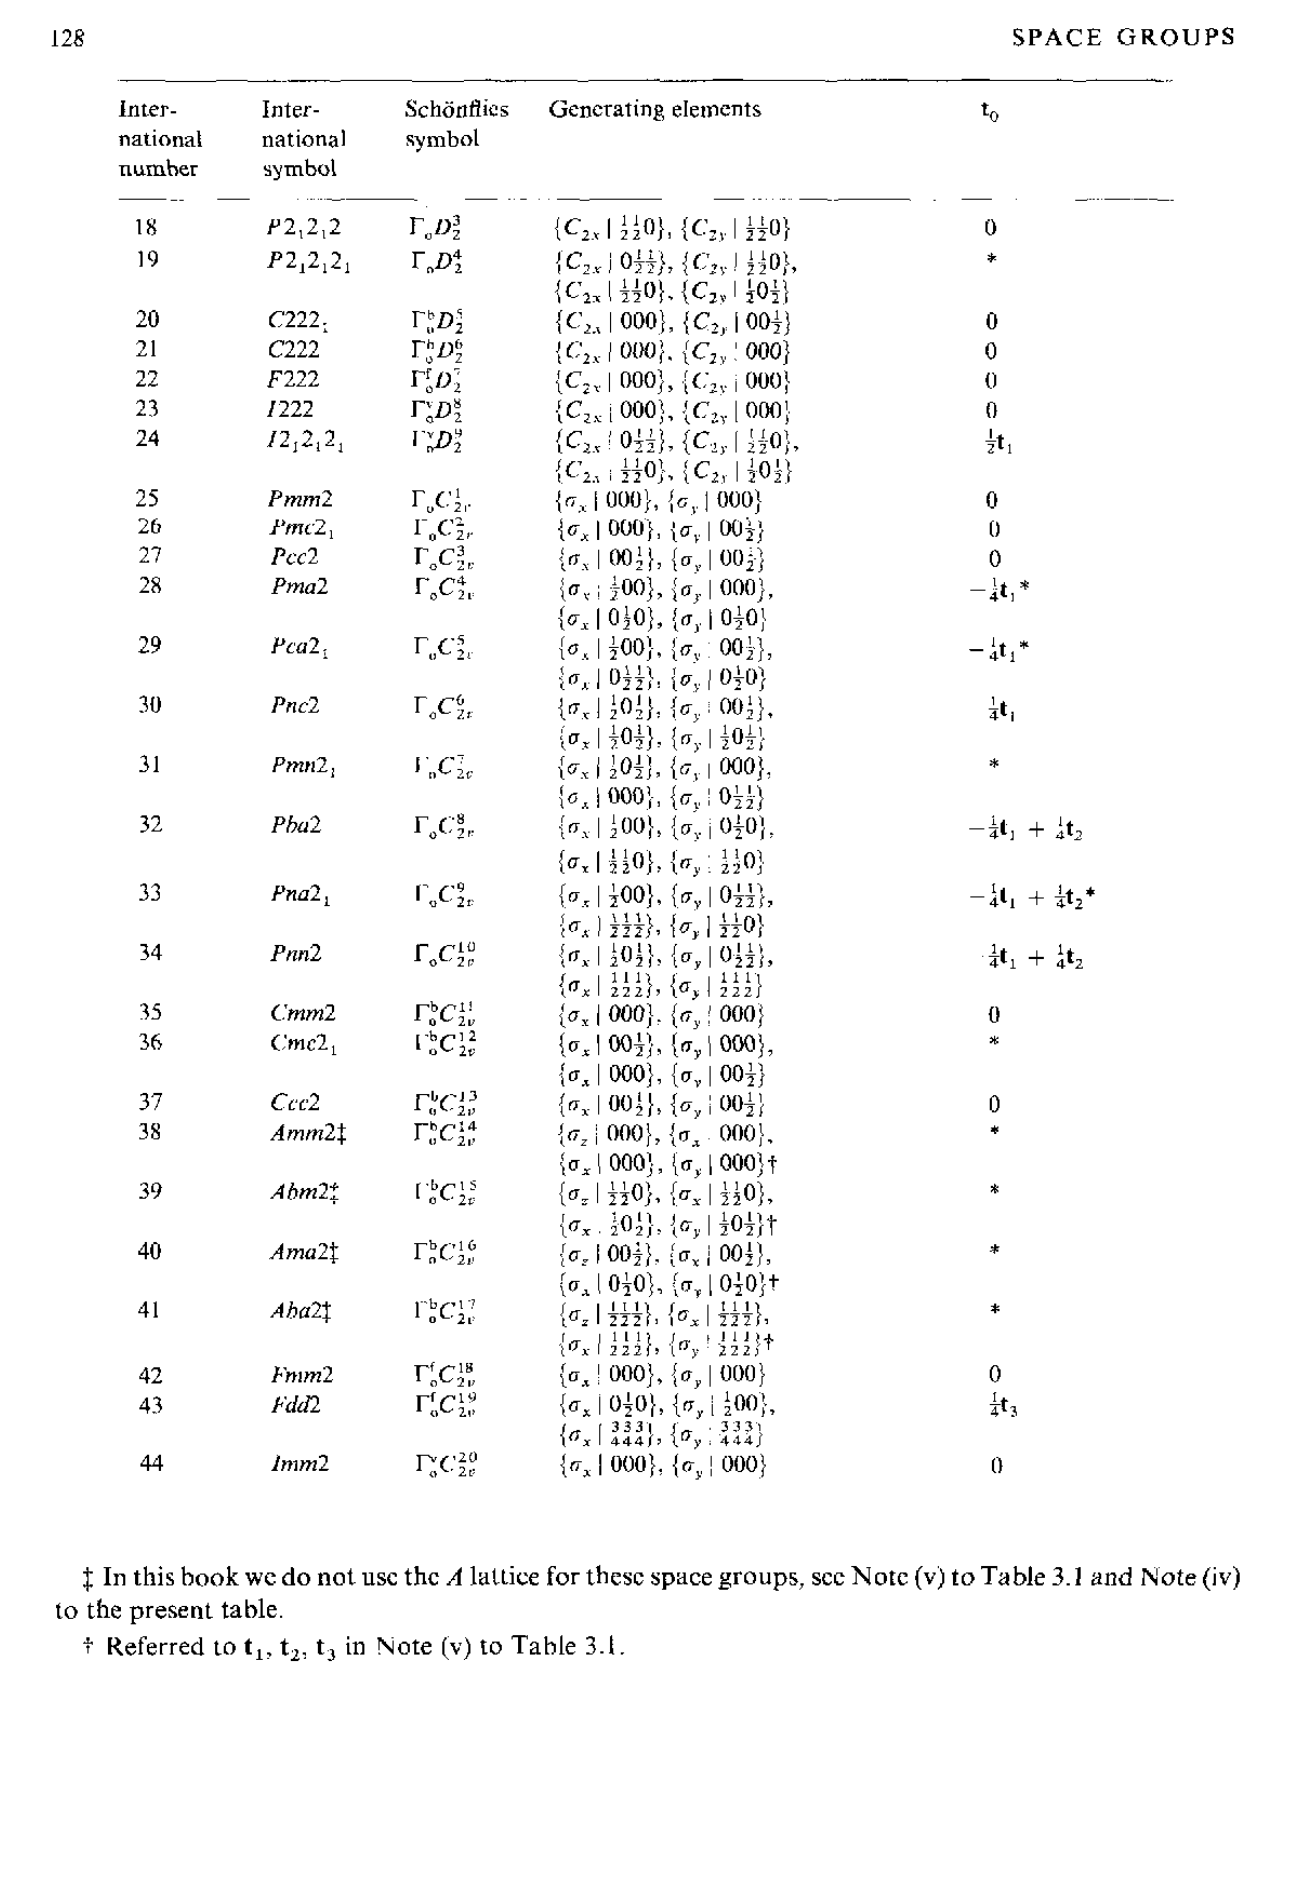
\includegraphics[width=0.92\textwidth]{c3_t37_p3.png}
\caption*{\textbf{表 3.7}（第 3 页）。}
\end{figure}
\begin{figure}[H]
\centering
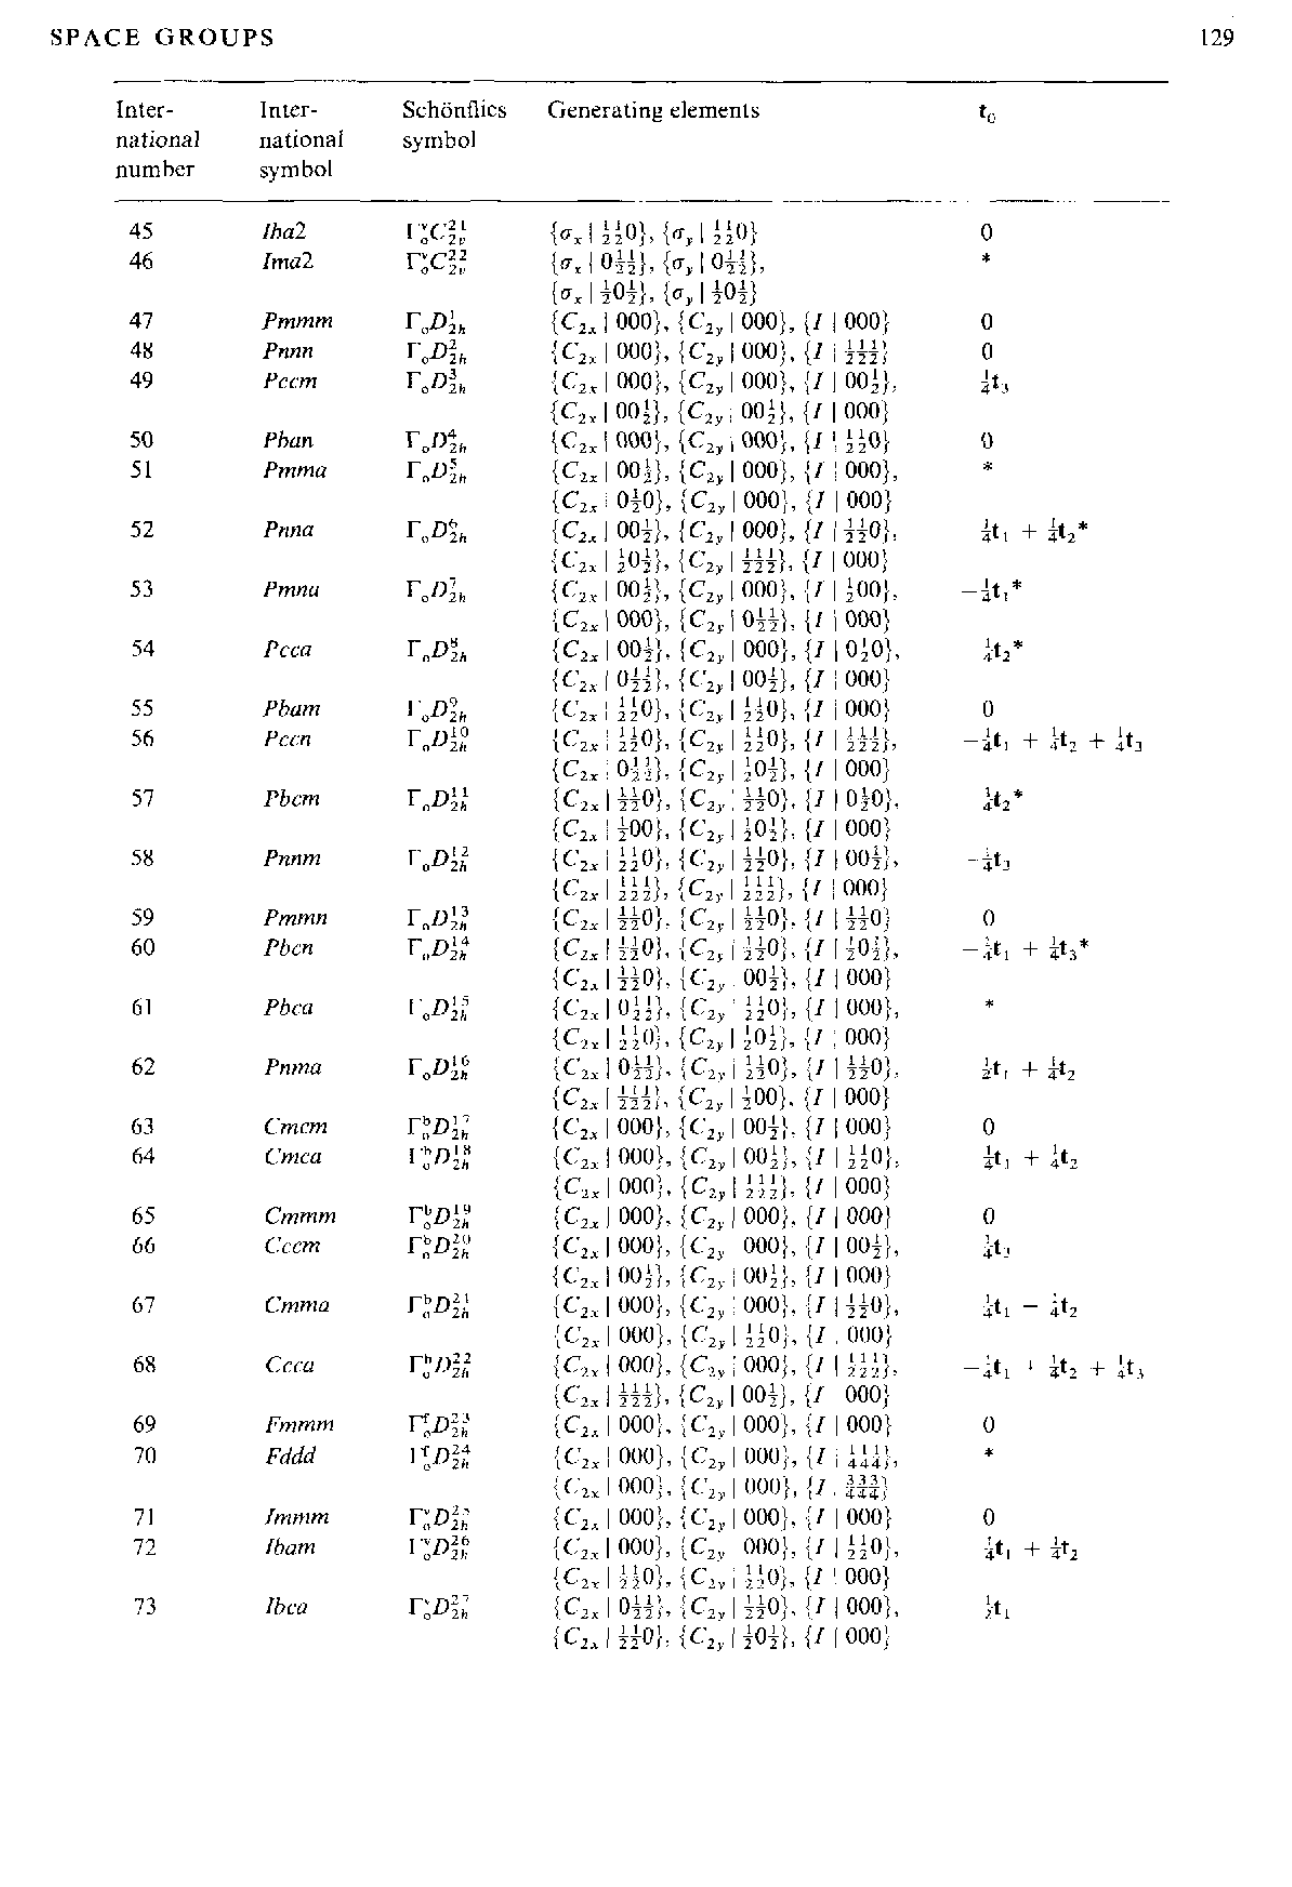
\includegraphics[width=0.92\textwidth]{c3_t37_p4.png}
\caption*{\textbf{表 3.7}（第 4 页）。}
\end{figure}
\begin{figure}[H]
\centering
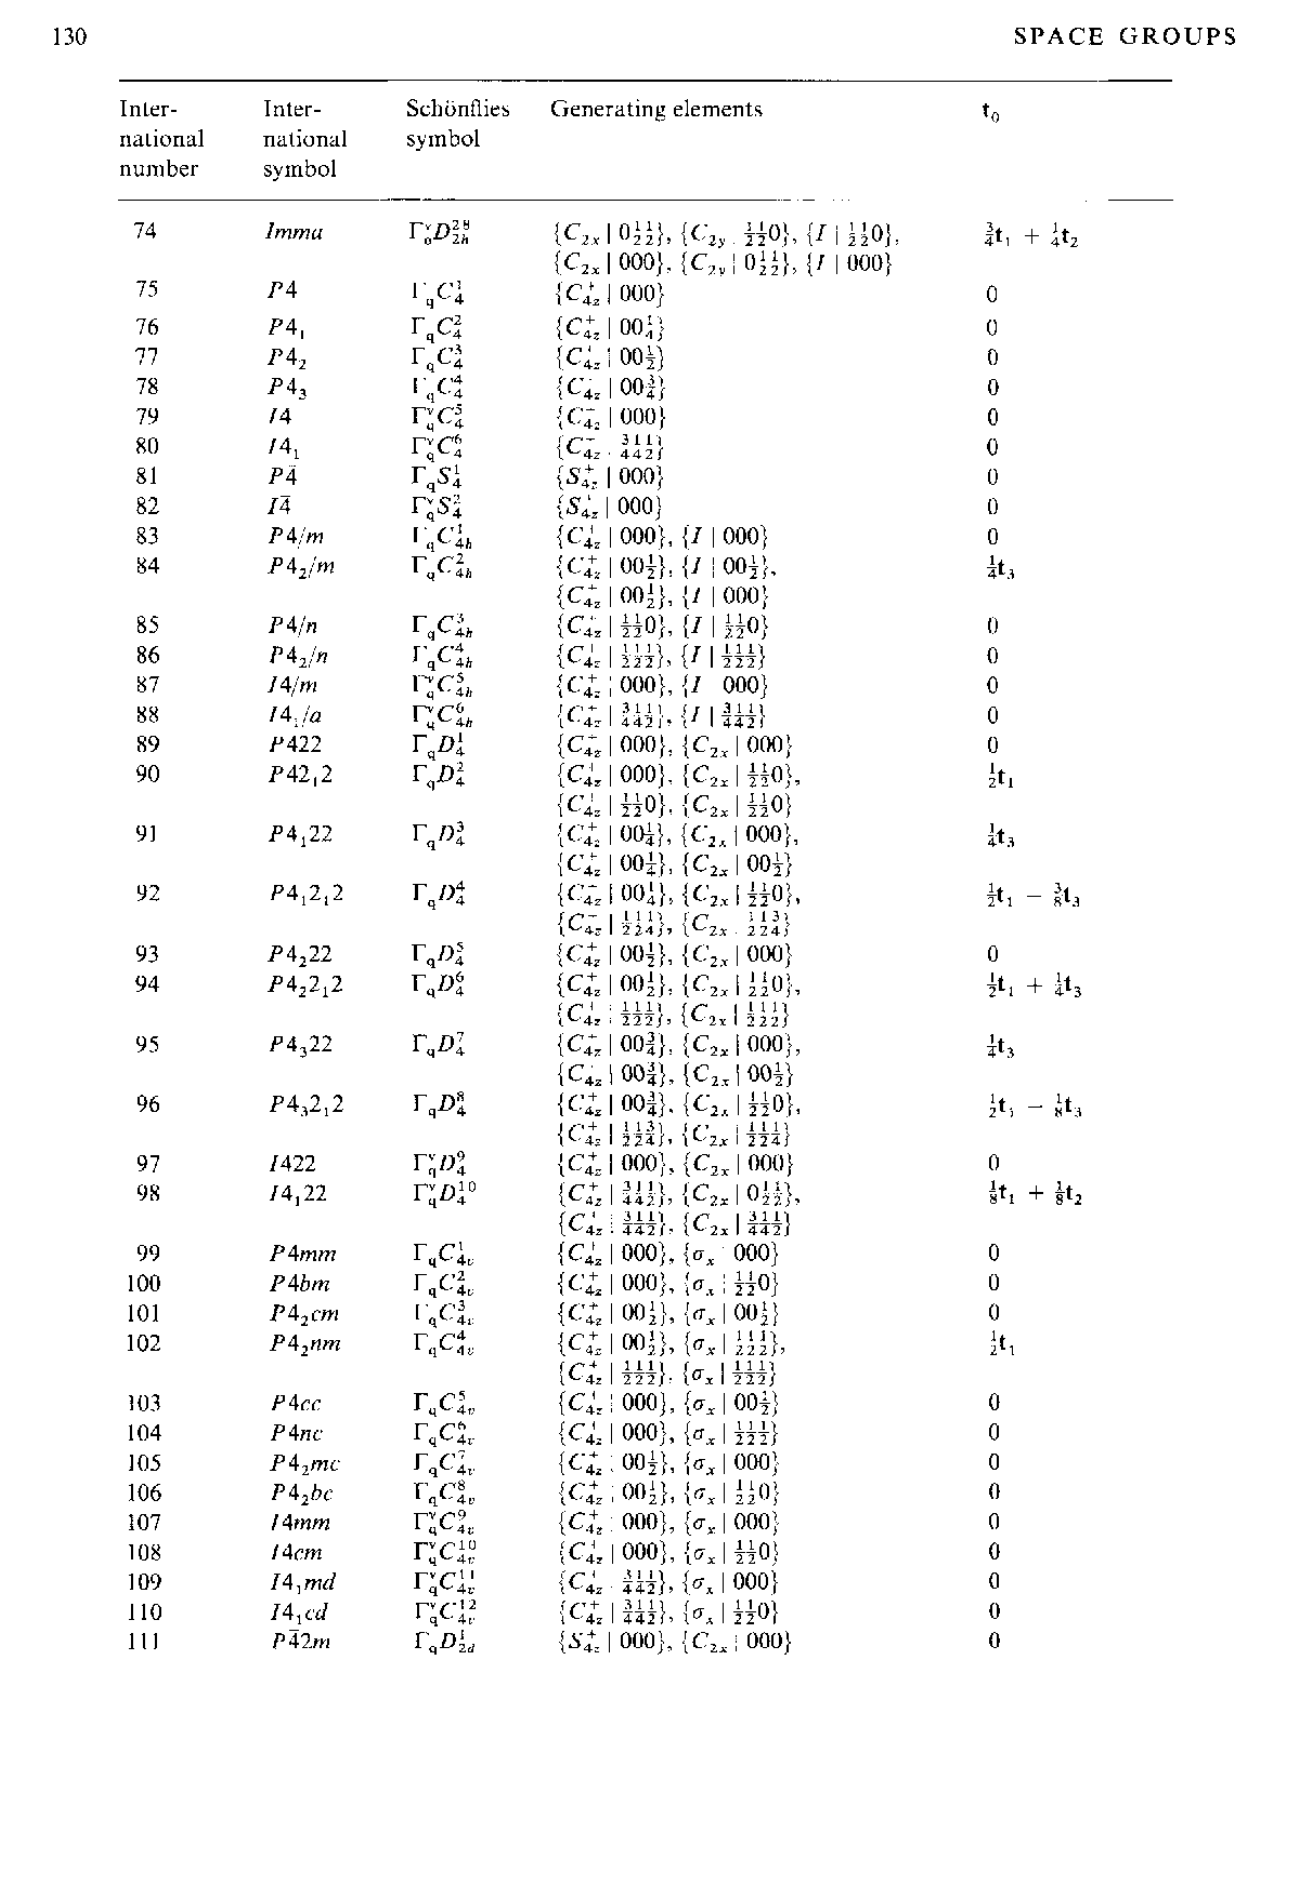
\includegraphics[width=0.92\textwidth]{c3_t37_p5.png}
\caption*{\textbf{表 3.7}（第 5 页）。}
\end{figure}
\begin{figure}[H]
\centering
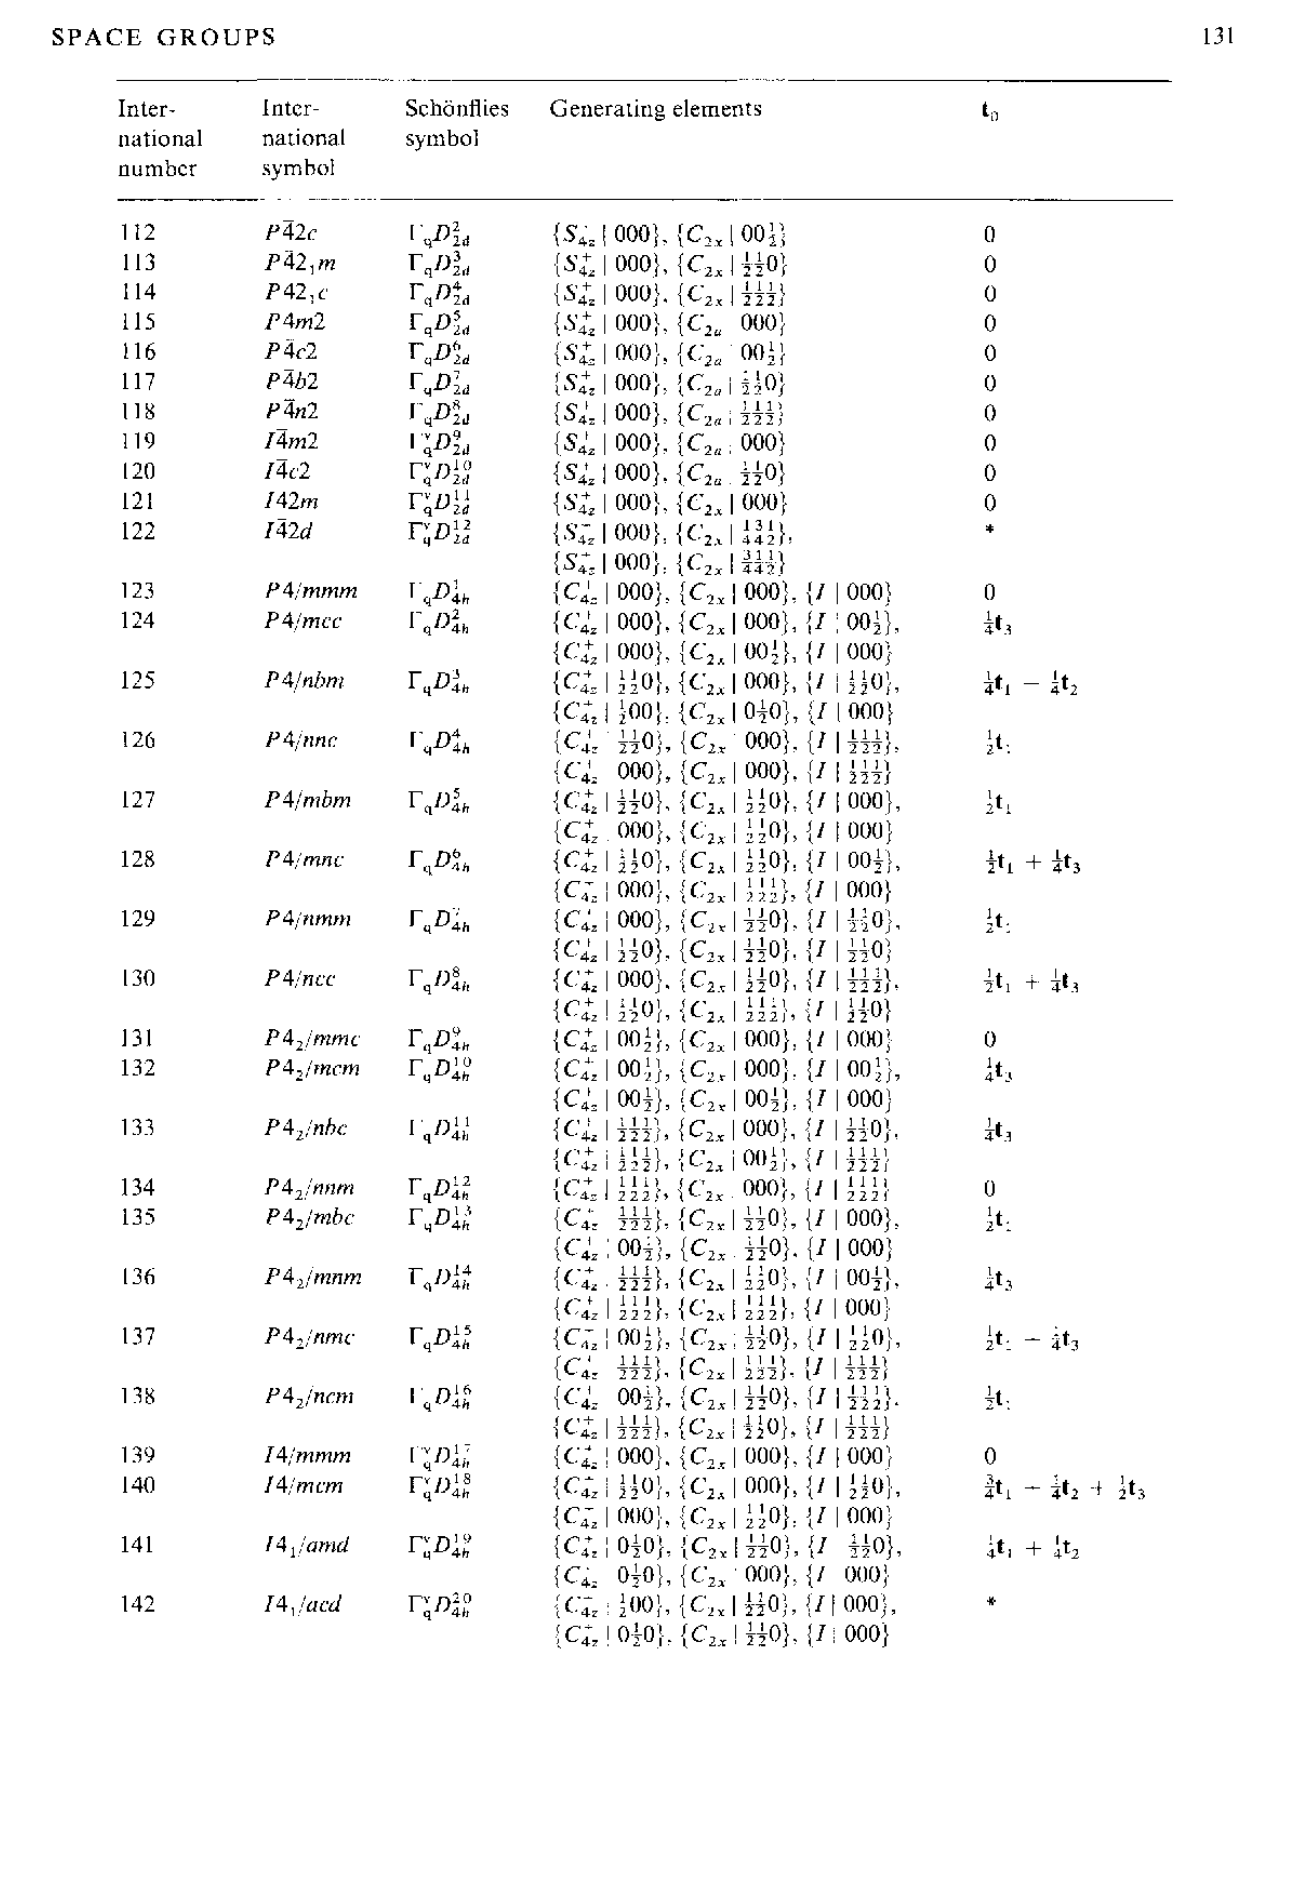
\includegraphics[width=0.92\textwidth]{c3_t37_p6.png}
\caption*{\textbf{表 3.7}（第 6 页）。}
\end{figure}
\begin{figure}[H]
\centering
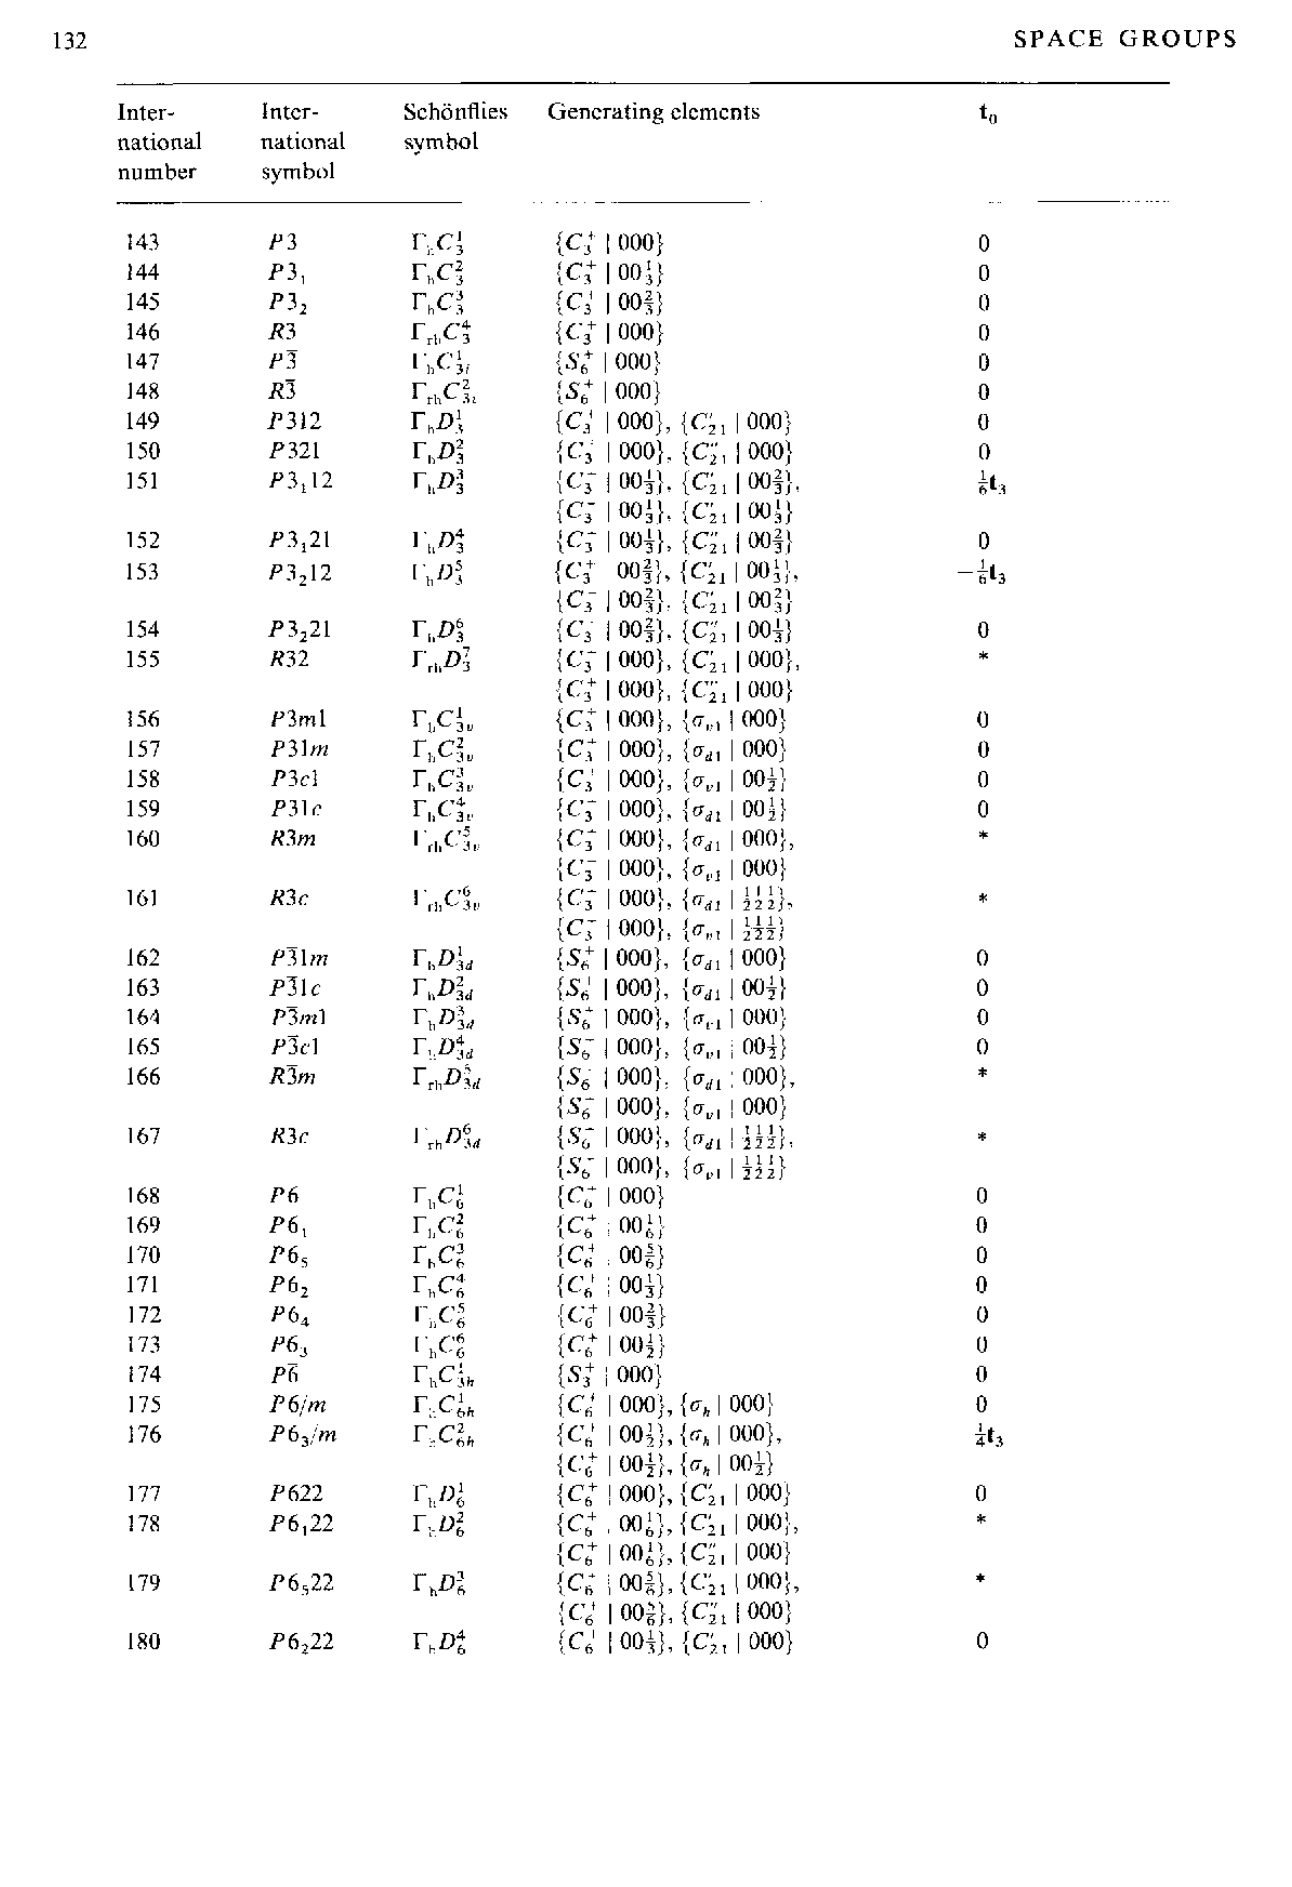
\includegraphics[width=0.92\textwidth]{c3_t37_p7.png}
\caption*{\textbf{表 3.7}（第 7 页）。}
\end{figure}
\begin{figure}[H]
\centering
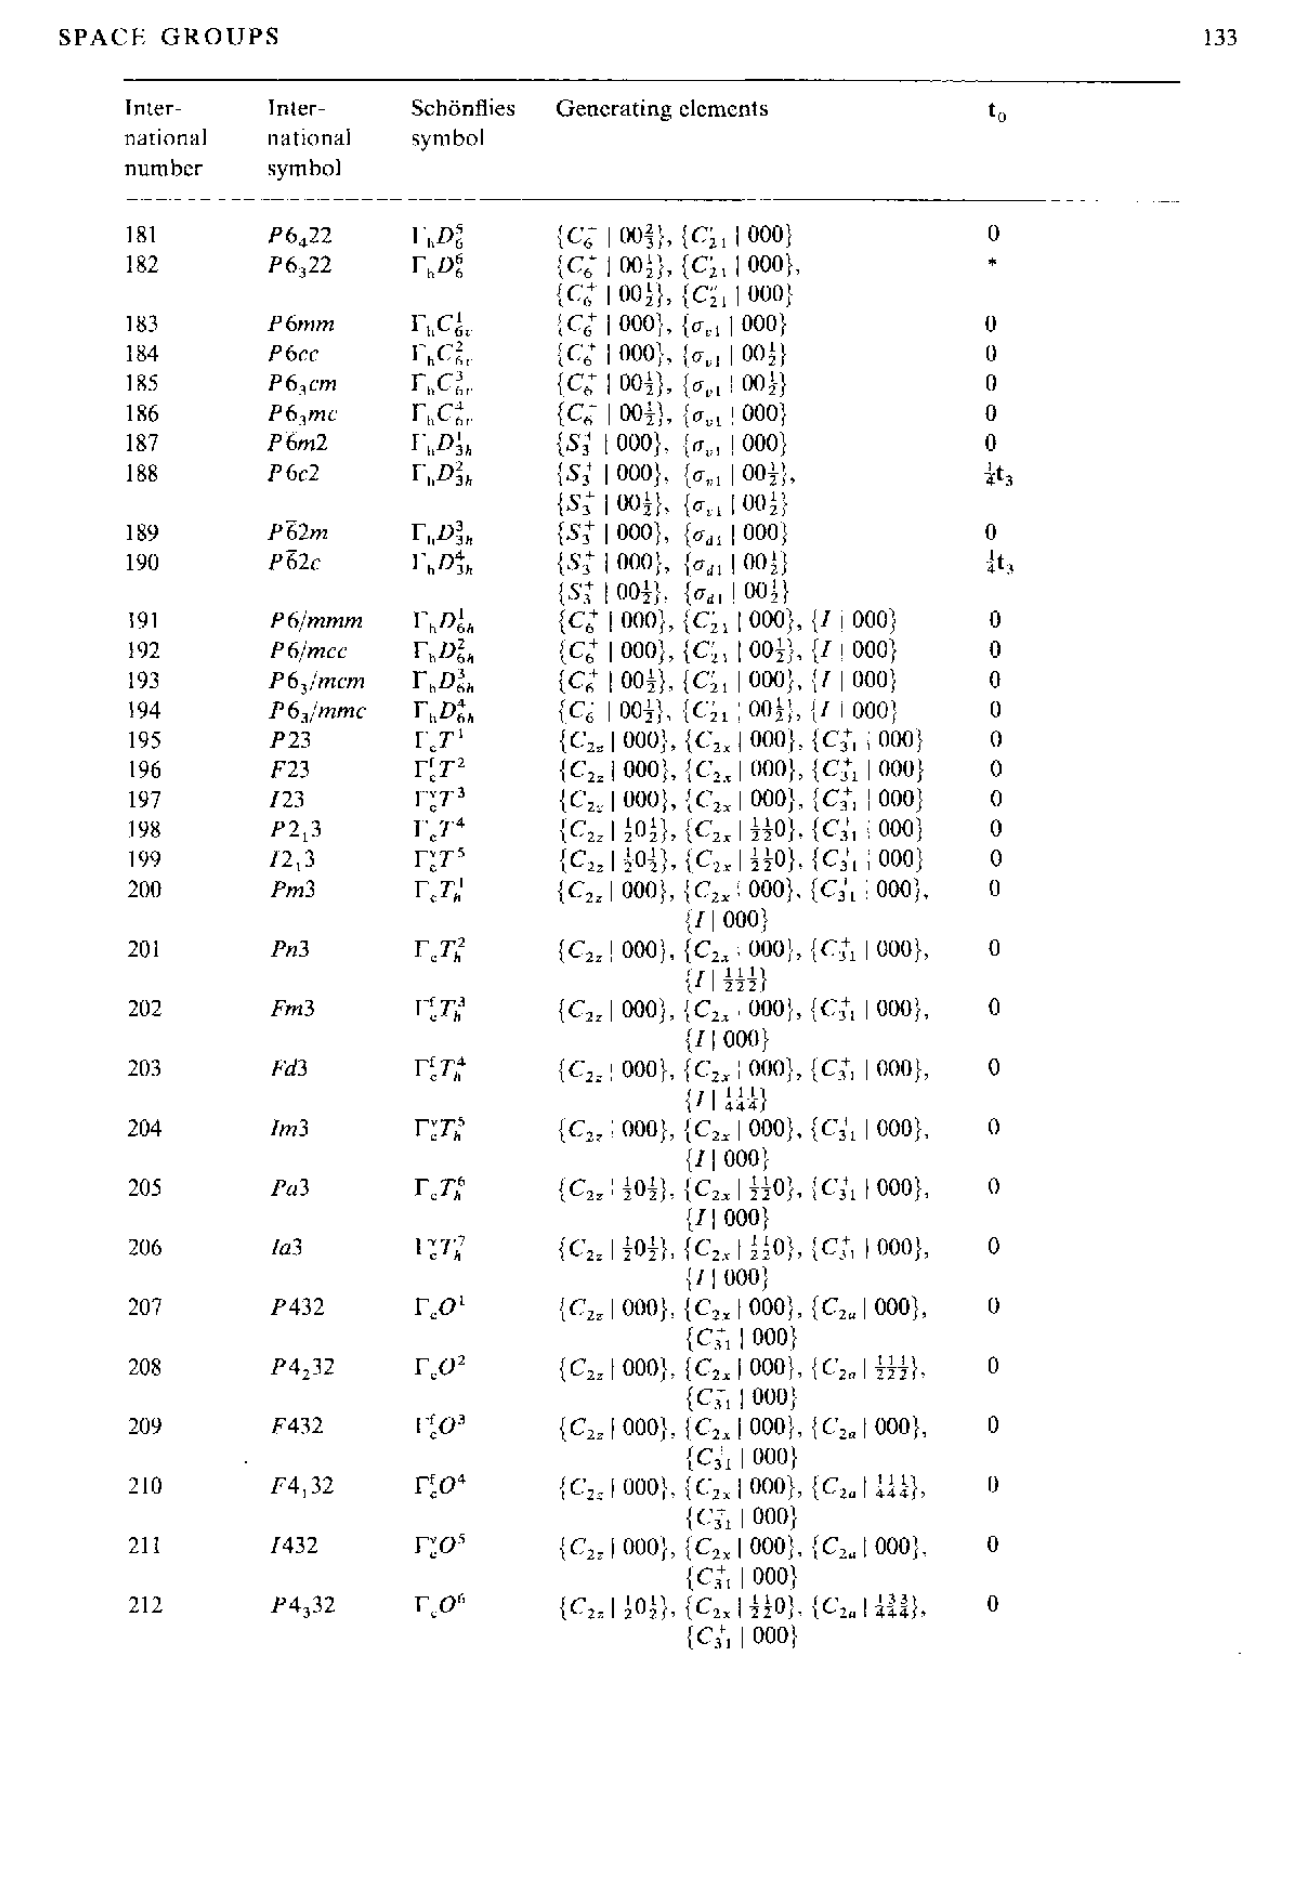
\includegraphics[width=0.92\textwidth]{c3_t37_p8.png}
\caption*{\textbf{表 3.7}（第 8 页，页末起为表的注）。}
\end{figure}
\begin{figure}[H]
\centering
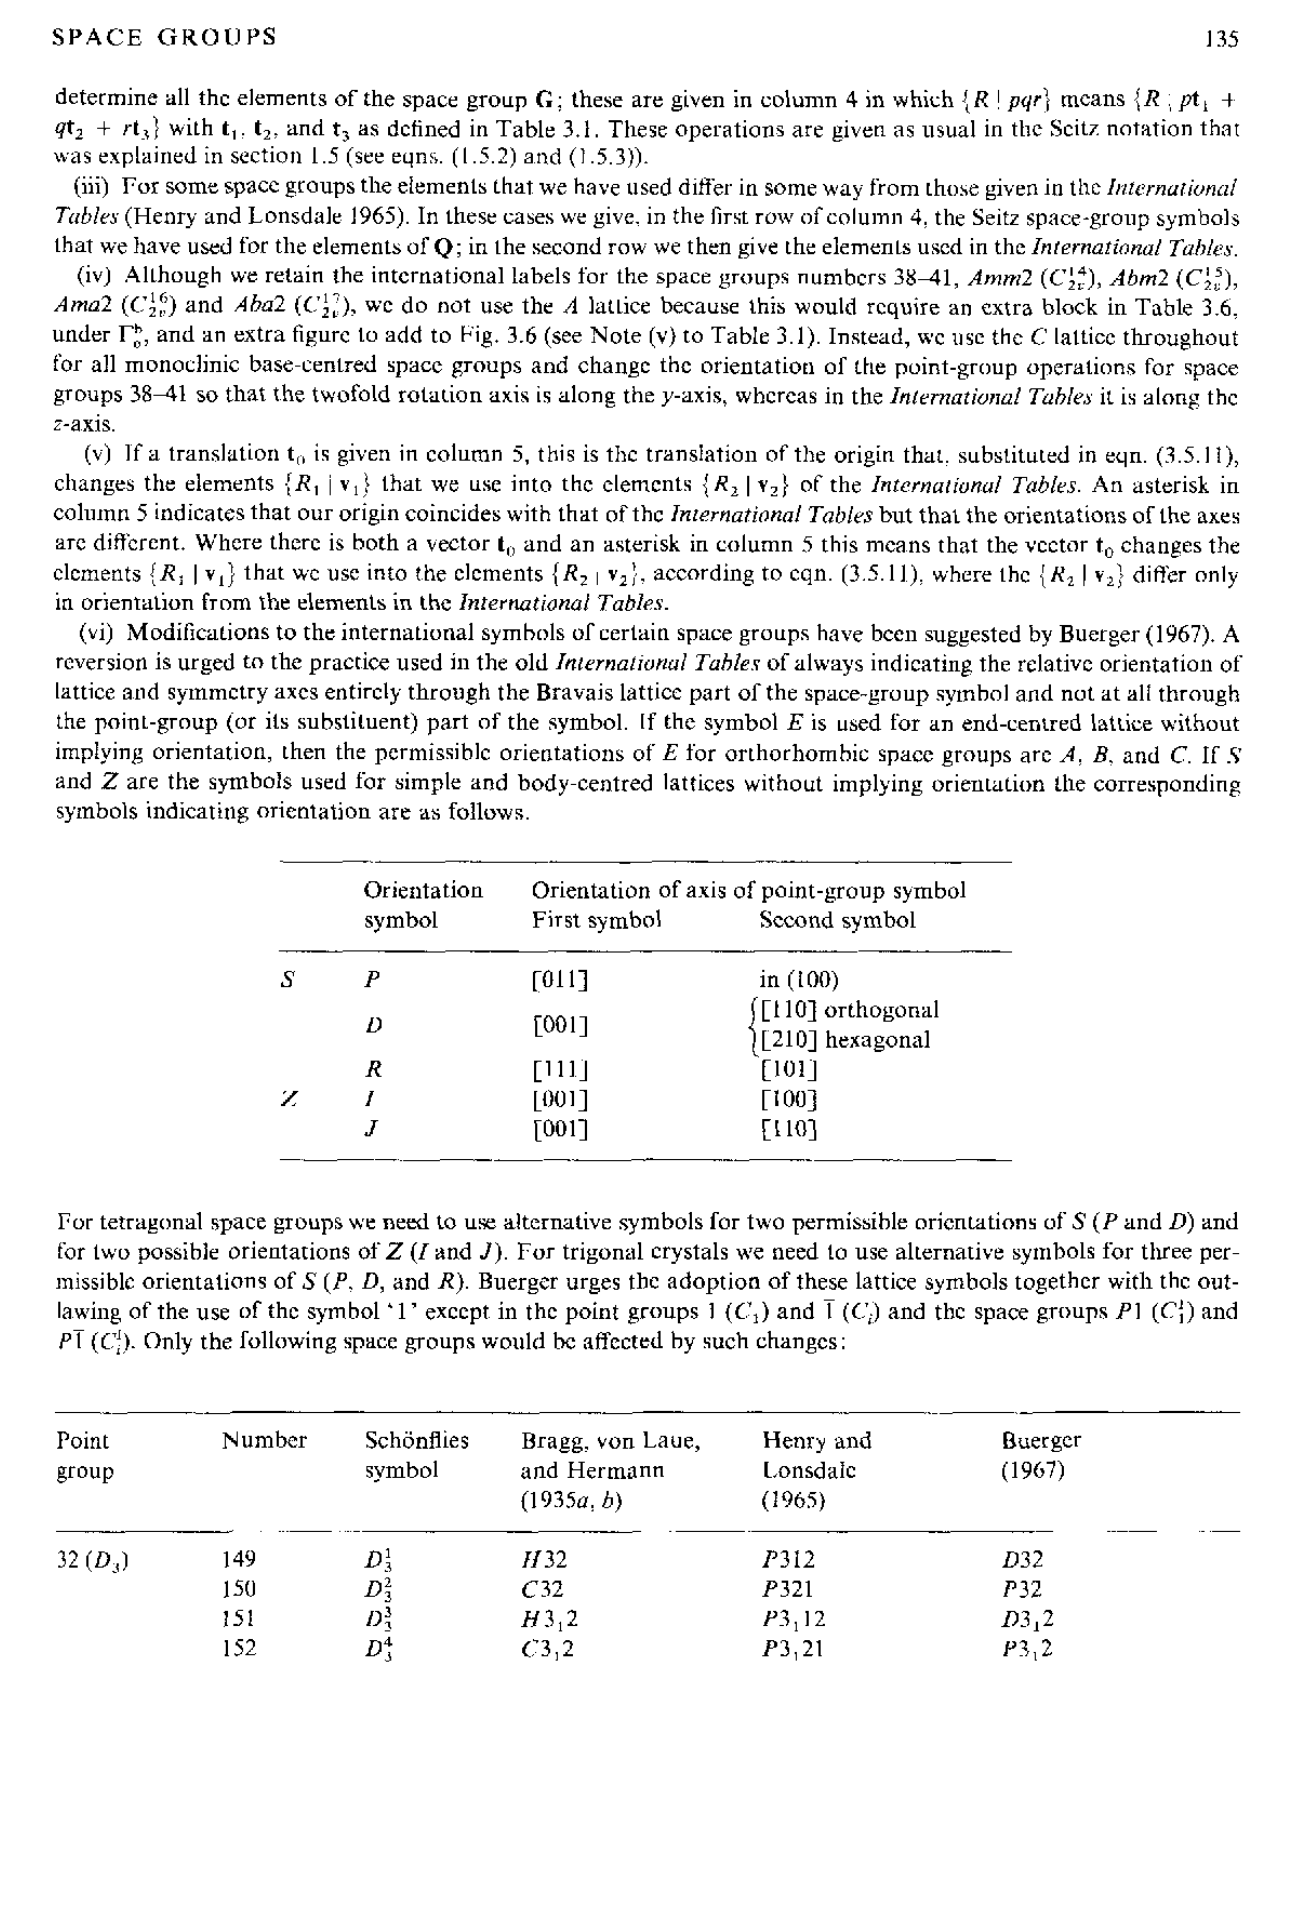
\includegraphics[width=0.92\textwidth]{c3_t37_p9.png}
\caption*{\textbf{表 3.7}（注 (ii) 续--(vi) 及取向符号表，原书扫描）。}
\end{figure}
\begin{figure}[H]
\centering
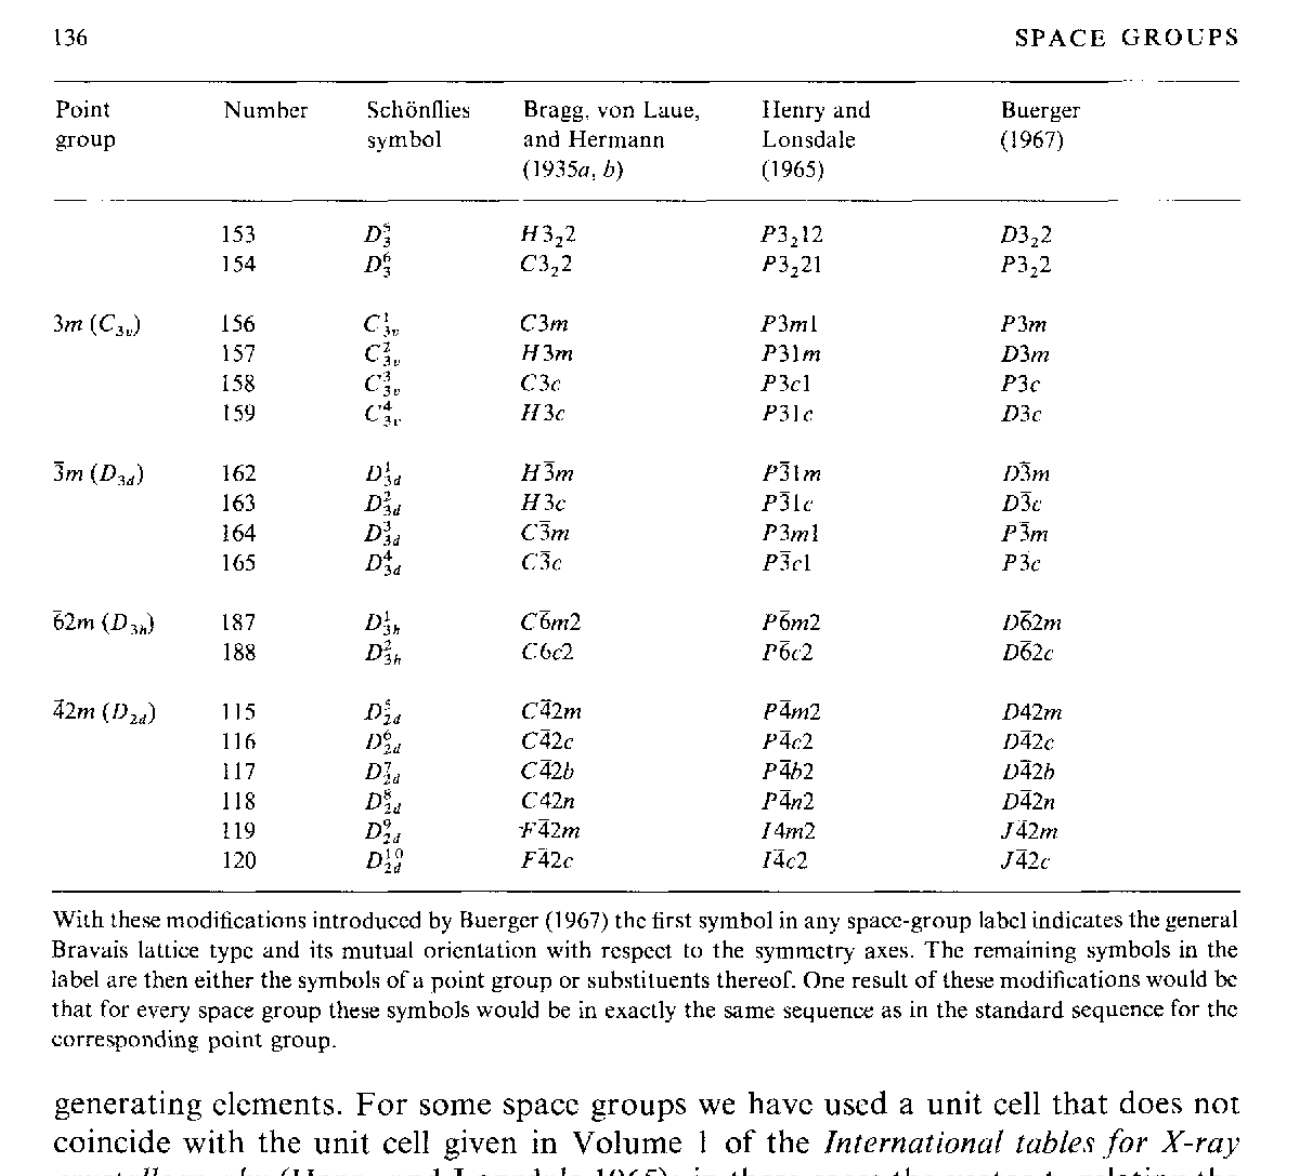
\includegraphics[width=0.80\textwidth]{c3_t37_p10.png}
\caption*{\textbf{表 3.7}（注 (vi) 附表：受 Buerger (1967) 建议影响的空间群，原书扫描）。}
\end{figure}

表 3.7 的注（译文）：

\noindent（i）我们在第 1、2、3 列中分别给出每个空间群的国际编号、国际符号和 Schönflies 符号。第 3 列的 Schönflies 符号前冠以相应布拉维格子的符号（见表 3.1）。

\noindent（ii）第 1、2、3 列给出的空间群名称蕴含（a）它所依托的布拉维格子，以及（b）同形点群。因此无需单独列出平移群 $\mathbf{T}$ 的元素（见表 3.1）或同形点群 $\mathbf{F}$ 的元素（见表 2.2）。尚需给出的是若干陪集代表（即 3.5 节所述 $\mathbf{Q}$ 的元素）。我们给出的数目足以确定空间群 $\mathbf{G}$ 的全部元素；这些元素列于第 4 列，其中 $\{R \mid pqr\}$ 表示 $\{R \mid p\mathbf{t}_{1} + q\mathbf{t}_{2} + r\mathbf{t}_{3}\}$，$\mathbf{t}_{1}$、$\mathbf{t}_{2}$、$\mathbf{t}_{3}$ 按表 3.1 的定义。这些操作一如既往地用 1.5 节解释的 Seitz 记号表示（见式 (1.5.2) 与 (1.5.3)）。

\noindent（iii）对某些空间群，我们所用的元素与《国际表》（Henry and Lonsdale 1965）所给的略有不同。对这些情形，我们在第 4 列的第一行给出我们用于 $\mathbf{Q}$ 的元素的 Seitz 空间群符号，第二行给出《国际表》所用的元素。

\noindent（iv）尽管我们保留编号 38--41（$Amm2\ (C_{2v}^{14})$、$Abm2\ (C_{2v}^{15})$、$Ama2\ (C_{2v}^{16})$、$Aba2\ (C_{2v}^{17})$）的国际记号，但不使用 A 格子，因为那将需要在表 3.6 的 $\Gamma_{o}^{b}$ 之下增加一个条目，并在图 3.6 中增加一幅图（见表 3.1 的注 (v)）。取而代之，我们对所有单斜底心空间群一律使用 C 格子，并把编号 38--41 的点群操作的取向改为使二次转动轴沿 $y$ 轴，而在《国际表》中它沿 $z$ 轴。

\noindent（v）若第 5 列给出一个平移 $\mathbf{t}_{0}$，则把它代入式 (3.5.11) 就能把我们所用的元素 $\{R_{1} \mid \mathbf{v}_{1}\}$ 变换为《国际表》的元素 $\{R_{2} \mid \mathbf{v}_{2}\}$。第 5 列中的星号表示我们的原点与《国际表》的原点重合，但轴的取向不同。若第 5 列既有矢量 $\mathbf{t}_{0}$ 又有星号，则表示矢量 $\mathbf{t}_{0}$ 按式 (3.5.11) 把我们所用的 $\{R_{1} \mid \mathbf{v}_{1}\}$ 变换为 $\{R_{2} \mid \mathbf{v}_{2}\}$，后者与《国际表》的元素只在取向上不同。

\noindent（vi）Buerger（1967）对某些空间群的国际符号提出了修改。他呼吁回到旧版《国际表》的做法：晶格与对称轴的相对取向完全由空间群符号中的布拉维格子部分表明，而完全不通过符号中的点群（或其替代）部分体现。若用符号 E 表示端心格子而不蕴含取向，则正交空间群中 E 的可取取向为 $A$、$B$ 和 $C$。若用 S 和 Z 表示简单和体心格子而不蕴含取向，则表明取向的相应符号如第 9 页扫描图中的表所示。对四方空间群，需要对 $S$ 的两种可取取向（P 和 D）以及 $Z$ 的两种可能取向（I 和 J）使用替代符号；对三方晶体，需要对 $S$ 的三种可取取向（P、D 和 R）使用替代符号。Buerger 敦促采用这些格子符号，并取缔符号“1”的使用——点群 $1\ (C_{1})$ 和 $\bar{1}\ (C_{i})$ 以及空间群 $P1\ (C_{1}^{1})$ 和 $P\bar{1}\ (C_{i}^{1})$ 除外。只有注 (vi) 附表中列出的空间群会受到这些改动的影响。经 Buerger（1967）引入这些修改后，任何空间群标签的第一个符号都表明布拉维格子的一般类型及其相对对称轴的取向，标签中其余的符号则要么是点群符号，要么是其替代符号。这些修改的一个结果是：对每个空间群，这些符号的顺序都将与相应点群的标准顺序完全一致。

空间群本身虽由《国际表》正式定义，但原点的选取和坐标轴取向的选择仍留有若干自由；《国际表》本身对许多空间群就给出了两种可替换的定向，正如 $Pmmn$（$D_{2h}^{13}$）的例子所示。援引《国际表》第 52 页的话：“所采用的空间群标准定向并不具有官方的重要性。”对某些空间群，《新国际表》（Henry and Lonsdale 1965）所用的空间群符号曾受到 Buerger（1967）的批评。Buerger 建议的修改已列于表 3.7 的注 (vi)；若被采纳，将只影响少数空间群。

国际空间群符号的逻辑在 1.5 节已有简要叙述。这些符号用于《国际表》第一版（Bragg, von Laue, and Hermann 1935\textit{a}, \textit{b}）并逐渐通用。当时符号的布拉维格子部分并不完全令人满意，因此在编纂新《国际表》时作了一些修改（Henry and Lonsdale 1965）；表 3.7 采用的就是新版符号。例如，四方点群 $\bar{4}2m$ 放进初基四方布拉维格子的晶胞时，纯转动轴既可以平行于 $x$ 轴，也可以平行于直线 $x = y$。旧《国际表》用两种不同的布拉维格子符号 P 和 C 区分这两种取向；对体心四方格子上的两种取向则用 I 和 F 两种符号。新《国际表》中，同一个布拉维格子在其一切空间群中都用同一符号表示（编号 38--41 的空间群 $Amm2\ (C_{2v}^{14})$、$Abm2\ (C_{2v}^{15})$、$Ama2\ (C_{2v}^{16})$、$Aba2\ (C_{2v}^{17})$ 除外）。点群在布拉维格子上不同取向的区分问题，于是或者通过调换点群符号 $\bar{4}2m$ 和 $\bar{6}2m$ 中最后两个符号的次序（得到 $\bar{4}m2$ 和 $\bar{6}m2$）来解决，或者对三方空间群通过把符号“1”加在空间群符号的不同位置来解决。其结果是，对称性符号如今常常被部分地理解为不仅表明有哪些对称元素，还表明其取向，见 Henry and Lonsdale（1965）的表 3.3.2。国际点群标记各部分的身份问题在第七章还会涉及。

为了说明如何用《国际表》给出的等价位置确定对称元素的几何描述，我们遵循 Wondratschek and Neubüser（1967）的方法。应当从 1.4 与 1.5 节清楚地区分\textit{对称元素}（如转动轴或对称面，粗略地说这是晶体的一种物理属性）与\textit{对称操作}（它是晶体的覆盖操作，是点群或空间群这一抽象数学群的元素）。空间群对称操作 $\{R_{i} \mid \mathbf{r}_{i}\}$ 作用在点 $x, y, z$ 上，产生等价位置中的某一点，后者一般可写为
\begin{equation*}
\begin{aligned}
x', y', z' &= r_{1} + a_{11}x + a_{12}y + a_{13}z,\\
&\quad r_{2} + a_{21}x + a_{22}y + a_{23}z,\ r_{3} + a_{31}x + a_{32}y + a_{33}z,
\end{aligned}
\tag{3.5.14}
\end{equation*}
其中 $r_{i}$ 是有理数，$a_{ij}$ 为 $+1$、$-1$ 或 0。

\noindent\textbf{例 3.5.1}\quad 在 $Pmmn$（$D_{2h}^{13}$）的诸等价位置中有 $\frac{1}{2}+x, \frac{1}{2}-y, \bar{z}$；这意味着 $a_{11} = +1$，$a_{22} = a_{33} = -1$，$r_{1} = r_{2} = \frac{1}{2}$，$r_{3} = 0$，其余 $a_{ij} = 0$。

式 (3.5.14) 可以方便地写成矩阵形式
\begin{equation*}
\mathbf{M}\left(\{R_{i} \mid \mathbf{r}_{i}\}\right) = \begin{pmatrix} a_{11} & a_{12} & a_{13} & r_{1}\\ a_{21} & a_{22} & a_{23} & r_{2}\\ a_{31} & a_{32} & a_{33} & r_{3}\\ 0 & 0 & 0 & 1 \end{pmatrix} = (\mathbf{A}, \mathbf{r}_{i})
\tag{3.5.15}
\end{equation*}
其中 $\mathbf{M}(\{R_{i} \mid \mathbf{r}_{i}\})$ 作用在列矢量 $(x, y, z, 1)^{\mathrm{T}}$ 上。显然矩阵 $a_{ij}$ 已经以缩并的形式出现在表 1.4 的 Jones 符号中。$\{R_{i} \mid \mathbf{r}_{i}\}$ 的 $R_{i}$ 部分的几何意义当然可以直接由表 1.4 辨认；另一种做法是，$\mathbf{A}$ 的特征标 $\chi(\mathbf{A})$ 与行列式 $\det(\mathbf{A})$ 很容易计算，按表 3.8，这两个量完全刻画了 $R_{i}$ 的性质（Bethe 1929），其中 $C_{n}$ 表示转角为 $2\pi/n$ 的转动。

\begin{table}[H]
\centering
\caption*{\textbf{表 3.8}\ 由 $\chi(\mathbf{A})$ 和 $\det(\mathbf{A})$ 确定 $R_{i}$ 的形式}
\begin{tabular}{@{}lcccccccccc@{}}
\toprule
$R_{i}$ & $C_{1}$ & $C_{2}$ & $C_{3}$ & $C_{4}$ & $C_{6}$ & $IC_{1}$ & $IC_{2}$ & $IC_{3}$ & $IC_{4}$ & $IC_{6}$\\
 & & & & & & $\equiv I$ & $\equiv\sigma$ & $\equiv S_{6}$ & $\equiv S_{4}$ & $\equiv S_{3}$\\
\midrule
$\chi(\mathbf{A})$ & $3$ & $-1$ & $0$ & $1$ & $2$ & $-3$ & $1$ & $0$ & $-1$ & $-2$\\
$\det(\mathbf{A})$ & $+1$ & $+1$ & $+1$ & $+1$ & $+1$ & $-1$ & $-1$ & $-1$ & $-1$ & $-1$\\
\bottomrule
\end{tabular}
\end{table}

若 $\det(\mathbf{A}) = +1$，则对称元素或者是纯转动轴，或者是螺旋转动轴。于是我们要确定该轴的方向；对螺旋转动轴，还要确定螺旋矢量 $\mathbf{w}$，即平移 $\mathbf{r}_{i}$ 沿轴方向的分量。若 $\mathbf{q}$ 是过原点且平行于螺旋轴的矢量，则 $\mathbf{A}\mathbf{q} = \mathbf{q}$，因此给出螺旋轴方向的 $\mathbf{q}$ 可由
\begin{equation*}
(\mathbf{A} - \mathbf{E})\mathbf{q} = 0
\tag{3.5.16}
\end{equation*}
求得。对螺旋转动，为确定 $\mathbf{w}$，注意
\begin{equation*}
\{R_{i} \mid \mathbf{r}_{i}\}\mathbf{q} = \mathbf{A}\mathbf{q} + \mathbf{r}_{i} = \mathbf{E}\mathbf{q} + \mathbf{r}_{i} = \mathbf{q} + \mathbf{r}_{i}
\tag{3.5.17}
\end{equation*}
因此
\begin{equation*}
\{R_{i} \mid \mathbf{r}_{i}\}^{2}\mathbf{q} = \mathbf{q} + \mathbf{r}_{i} + \mathbf{A}\mathbf{r}_{i}
\tag{3.5.18}
\end{equation*}
且
\begin{equation*}
\begin{aligned}
\{R_{i} \mid \mathbf{r}_{i}\}^{n}\mathbf{q} &= \mathbf{q} + \mathbf{r}_{i} + \mathbf{A}\mathbf{r}_{i} + \mathbf{A}^{2}\mathbf{r}_{i} + \dots + \mathbf{A}^{n-1}\mathbf{r}_{i}\\
&= \mathbf{q} + n\mathbf{w}
\end{aligned}
\tag{3.5.19}
\end{equation*}
因为 $n$ 次螺旋转动操作等价于纯平移 $n\mathbf{w}$。整理式 (3.5.19) 得螺旋矢量 $\mathbf{w}$ 的显式表达式
\begin{equation*}
\mathbf{w} = (1/n)(\mathbf{E} + \mathbf{A} + \mathbf{A}^{2} + \dots + \mathbf{A}^{n-1})\mathbf{r}_{i}.
\tag{3.5.20}
\end{equation*}
螺旋轴的方向当然由 $\mathbf{w}$ 的方向给出，但由式 (3.5.16) 更容易求得该方向。轴的定位则可由“轴上的点 $\mathbf{x}$ 满足 $\mathbf{A}\mathbf{x} + \mathbf{r}_{i} = \mathbf{x} + \mathbf{w}$”这一事实确定，即
\begin{equation*}
(\mathbf{A} - \mathbf{E})\mathbf{x} = \left(\frac{1}{n}\mathbf{B} - \mathbf{E}\right)\mathbf{r}_{i}
\tag{3.5.21}
\end{equation*}
其中
\begin{equation*}
\mathbf{B} = \mathbf{E} + \mathbf{A} + \mathbf{A}^{2} + \dots + \mathbf{A}^{n-1}.
\tag{3.5.22}
\end{equation*}
若 $n = 2$，式 (3.5.21) 有特别简单的解 $\mathbf{x} = \frac{1}{2}\mathbf{r}_{i}$。若 $\det(\mathbf{A}) = -1$，则要考虑三种可能的情形：(a) $I\ ( = IC_{1})$；(b) $\sigma\ ( = IC_{2})$；(c) $S_{6}\ ( = IC_{3})$；$S_{4}\ ( = IC_{4})$；以及 $S_{3}\ ( = IC_{6})$。

\noindent(a) $I\ ( = IC_{1})$。反演中心 $\mathbf{x}$ 可由 $\mathbf{x} = \{I \mid \mathbf{r}_{i}\}\mathbf{x} = -\mathbf{x} + \mathbf{r}_{i}$ 求得，故 $\mathbf{x} = \frac{1}{2}\mathbf{r}_{i}$。

\noindent(b) $\sigma\ ( = IC_{2})$。平面的取向可以用一个过原点且垂直于该平面的矢量 $\mathbf{q}$ 描述；$\mathbf{q}$ 满足 $\mathbf{A}\mathbf{q} = -\mathbf{q}$，即
\begin{equation*}
(\mathbf{A} + \mathbf{E})\mathbf{q} = 0.
\tag{3.5.23}
\end{equation*}
对滑移面，滑移矢量 $\mathbf{w}$ 可由下述事实求得：把 $\{R_{i} \mid \mathbf{r}_{i}\}$ 相继作用两次于平面内的点 $\mathbf{x}$，把它移到 $\mathbf{x} + 2\mathbf{w}$，于是由式 (3.5.18)，
\begin{equation*}
\{R_{i} \mid \mathbf{r}_{i}\}^{2}\mathbf{x} = \mathbf{x} + \mathbf{r}_{i} + \mathbf{A}\mathbf{r}_{i} = \mathbf{x} + 2\mathbf{w}.
\tag{3.5.24}
\end{equation*}
因此
\begin{equation*}
\mathbf{w} = \frac{1}{2}(\mathbf{A} + \mathbf{E})\mathbf{r}_{i}.
\tag{3.5.25}
\end{equation*}
平面内任一点 $\mathbf{x}$ 满足 $\{R_{i} \mid \mathbf{r}_{i}\}\mathbf{x} = \mathbf{A}\mathbf{x} + \mathbf{r}_{i} = \mathbf{x} + \mathbf{w}$，故 $\mathbf{x}$ 满足
\begin{equation*}
(\mathbf{A} - \mathbf{E})\mathbf{x} = \frac{1}{2}(\mathbf{A} - \mathbf{E})\mathbf{r}_{i},
\tag{3.5.26}
\end{equation*}
它显然有特解 $\mathbf{x} = \frac{1}{2}\mathbf{r}_{i}$。

\noindent(c) $S_{6}\ ( = IC_{3})$；$S_{4}\ ( = IC_{4})$；$S_{3}\ ( = IC_{6})$。若 $\mathbf{q}$ 是过原点且平行于其中某根轴的矢量，则 $\mathbf{A}\mathbf{q} = -\mathbf{q}$，$\mathbf{q}$ 同样由求解
\begin{equation*}
(\mathbf{A} + \mathbf{E})\mathbf{q} = 0.
\tag{3.5.23}
\end{equation*}
得到。\footnote{中译者注：原书对情形 (b) 与 (c) 重复使用了编号 (3.5.23)，照录。}不存在螺旋矢量 $\mathbf{w}$。反演中心可由 $\{R_{i} \mid \mathbf{r}_{i}\}\mathbf{x} = \mathbf{A}\mathbf{x} + \mathbf{r}_{i} = \mathbf{x}$ 求得，即
\begin{equation*}
(\mathbf{E} - \mathbf{A})\mathbf{x} = \mathbf{r}_{i}.
\tag{3.5.27}
\end{equation*}

在《国际表》中每个矩阵 $\mathbf{A}$ 都属于表 3.9 所示的四种不同类型之一。确定了 $R_{i}$ 的形式和 $\mathbf{A}$ 的类型之后，就可以利用表 3.10（它用到式 (3.5.16)--(3.5.27)）来确定与《国际表》中该空间群每个等价位置相对应的对称元素的取向和位置。

\begin{table}[H]
\centering
\caption*{\textbf{表 3.9}\ 由《X 射线晶体学国际表》产生的矩阵 $\mathbf{A}$ 的类型}
\begin{tabular}{@{}ll@{}}
\toprule
(i) & $\mathbf{A} = \begin{pmatrix} +1 & 0 & 0\\ 0 & \pm 1 & 0\\ 0 & 0 & \pm 1 \end{pmatrix}$；\qquad
(iii) (a) $\mathbf{A} = \begin{pmatrix} 0 & 0 & \pm 1\\ +1 & 0 & 0\\ 0 & \pm 1 & 0 \end{pmatrix}$，\\[3ex]
(ii) (a) & $\mathbf{A} = \begin{pmatrix} \pm 1 & 0 & 0\\ 0 & 0 & \pm 1\\ 0 & -1 & 0 \end{pmatrix}$，\qquad\quad
(b) $\mathbf{A} = \begin{pmatrix} 0 & \pm 1 & 0\\ 0 & 0 & \pm 1\\ +1 & 0 & 0 \end{pmatrix}$；\\[3ex]
(b) & $\mathbf{A} = \begin{pmatrix} 0 & 0 & \pm 1\\ 0 & \pm 1 & 0\\ \pm 1 & 0 & 0 \end{pmatrix}$，\qquad\quad
(iv) $\mathbf{A} = \begin{pmatrix} a_{11} & a_{12} & 0\\ a_{21} & a_{22} & 0\\ 0 & 0 & \pm 1 \end{pmatrix}$\quad
其中有一个 $a_{ik} = 0$，\\
\multicolumn{2}{l}{其余三个 $a_{ik} = \pm 1$；$i, k = 1, 2$。}\\
\bottomrule
\end{tabular}
\end{table}

\noindent\textbf{表 3.9 的注}\quad（i）假定采用的是 Henry and Lonsdale（1965）给出的定向；对其他定向，将不得不求解式 (3.5.16)--(3.5.27) 中的相应方程。

\begin{figure}[H]
\centering
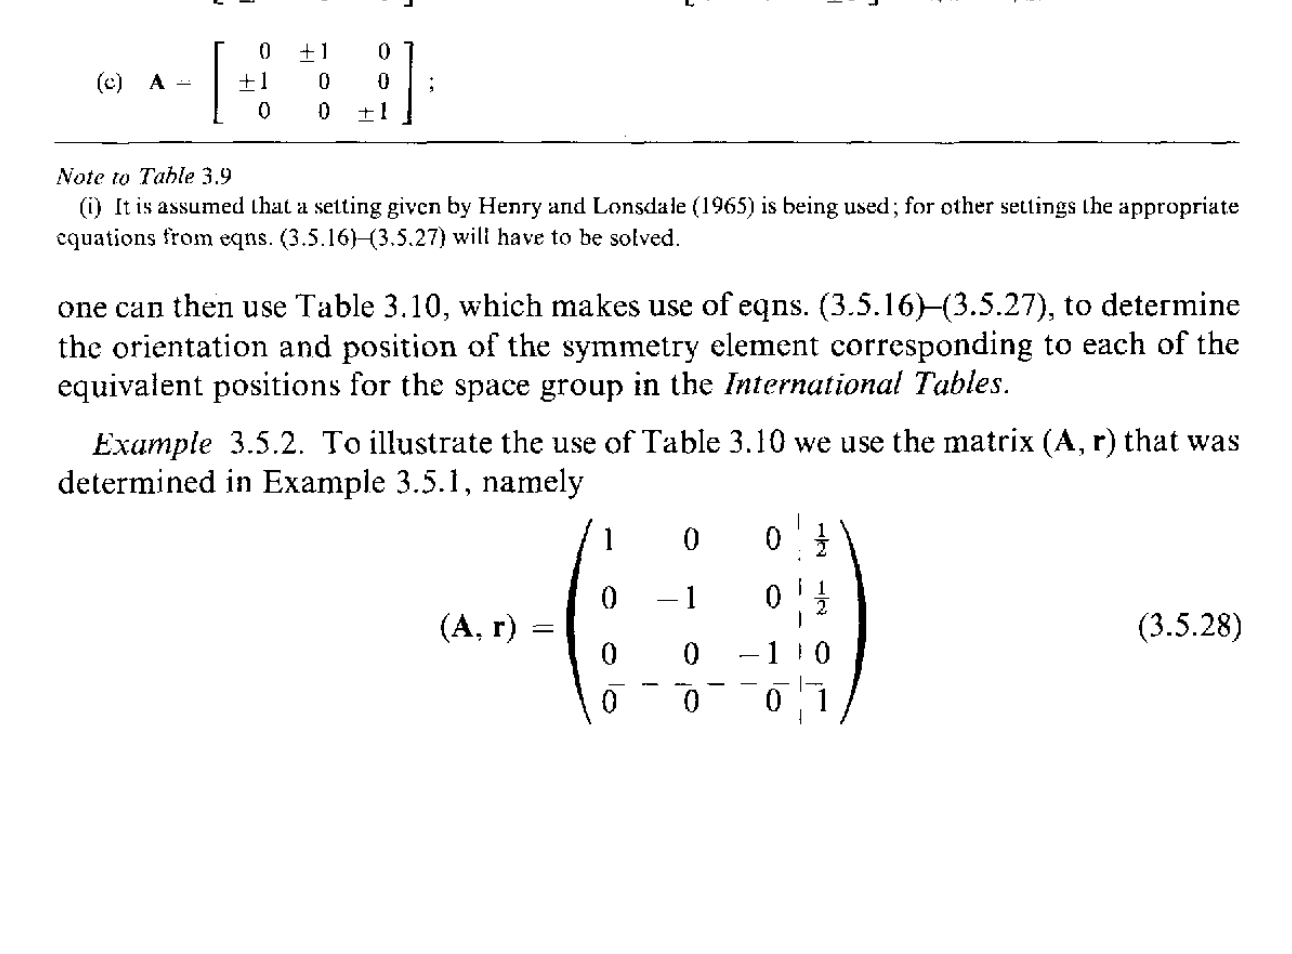
\includegraphics[width=0.92\textwidth]{c3_t310_p1.png}
\caption*{\textbf{表 3.10}\ 对称元素的测定（据 Wondratschek and Neubüser (1967)，原书第 140 页起扫描；第 1 页）。}
\end{figure}
\begin{figure}[H]
\centering
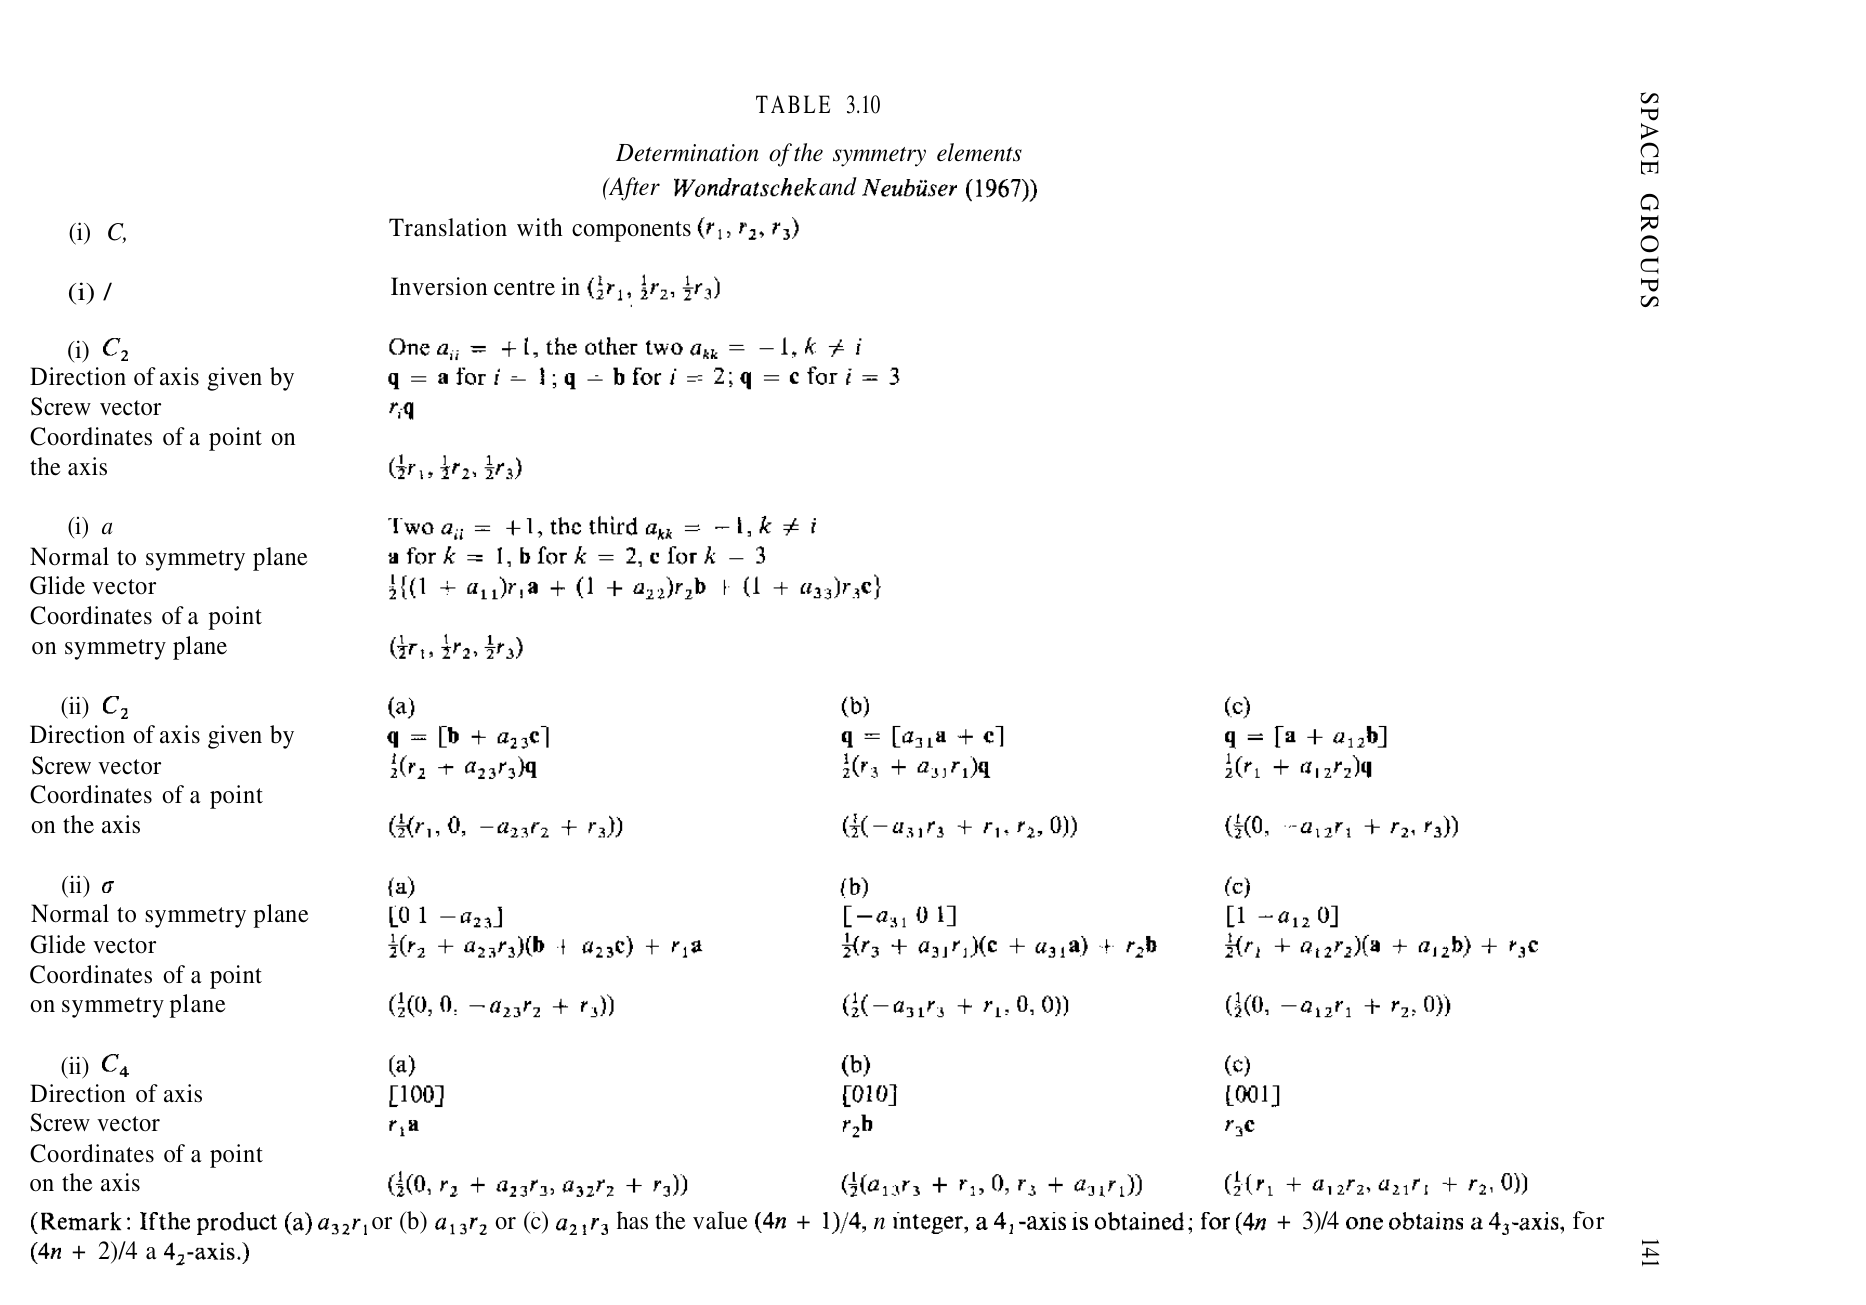
\includegraphics[width=0.92\textwidth]{c3_t310_p2.png}
\caption*{\textbf{表 3.10}（第 2 页）。}
\end{figure}
\begin{figure}[H]
\centering
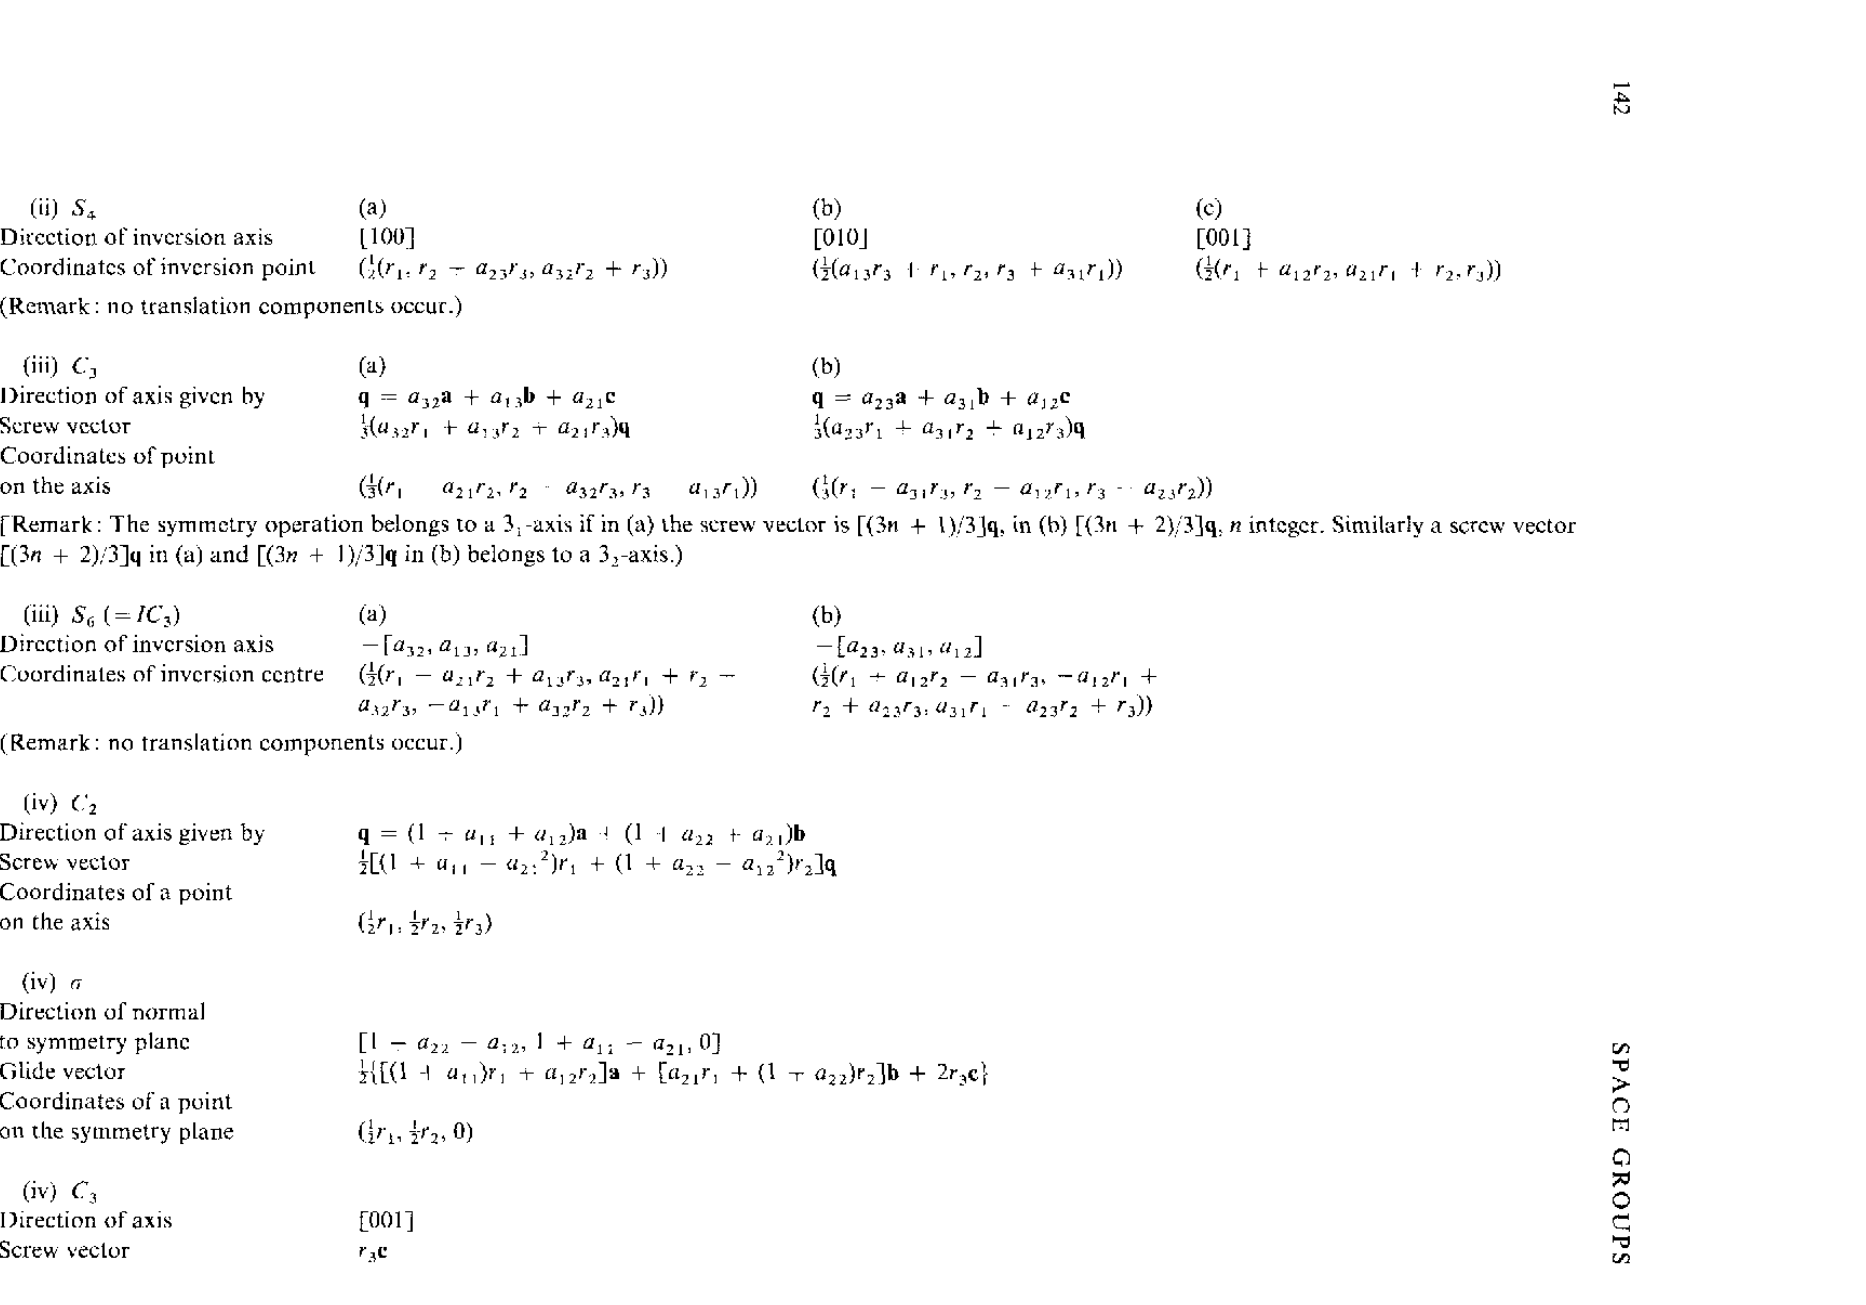
\includegraphics[width=0.92\textwidth]{c3_t310_p3.png}
\caption*{\textbf{表 3.10}（第 3 页，页末为表的注）。}
\end{figure}

表 3.10 的注（译文）：

\noindent（i）与《国际表》一致，$a$、$b$、$c$ 是惯用晶胞交于一个顶点的三条棱的长度；$\mathbf{a}$、$\mathbf{b}$、$\mathbf{c}$ 是沿这些棱的矢量。

\noindent（ii）矩阵 $\mathbf{A}(a_{ij})$ 与矢量 $\mathbf{r}_{i}$ 在正文中定义，见式 (3.5.14) 与 (3.5.15)。

\noindent（iii）$\mathbf{A}$ 的类型（i）、（ii）、（iii）或（iv）要用表 3.9 确定。

\noindent（iv）$C_{n}$ 是转角为 $2\pi/n$ 的纯转动。

\noindent（v）本表适用于 Henry and Lonsdale（1965）给出的晶胞定向；对其他定向，将不得不求解式 (3.5.16)--(3.5.27) 中的相应方程。

\noindent\textbf{例 3.5.2}\quad 为了说明表 3.10 的用法，我们用在例 3.5.1 中确定的矩阵 $(\mathbf{A}, \mathbf{r})$：
\begin{equation*}
(\mathbf{A}, \mathbf{r}) = \begin{pmatrix} 1 & 0 & 0 & \frac{1}{2}\\ 0 & -1 & 0 & \frac{1}{2}\\ 0 & 0 & -1 & 0\\ 0 & 0 & 0 & 1 \end{pmatrix}
\tag{3.5.28}
\end{equation*}
于是
\begin{equation*}
\mathbf{A} = \begin{pmatrix} 1 & 0 & 0\\ 0 & -1 & 0\\ 0 & 0 & -1 \end{pmatrix}
\tag{3.5.29}
\end{equation*}
从而
\begin{equation*}
\chi(\mathbf{A}) = -1
\tag{3.5.30}
\end{equation*}
且
\begin{equation*}
\det(\mathbf{A}) = +1.
\tag{3.5.31}
\end{equation*}
由表 3.8，$\{R_{i} \mid \mathbf{r}_{i}\}$ 是一个 $C_{2}$ 型转动；再由表 3.10，由于 $i = 1$，它沿 $x$ 方向，即 $C_{2x}$。螺旋矢量的方向为 $\mathbf{r}_{1}\mathbf{q} = \frac{1}{2}\mathbf{a}$，轴的位置由其通过点 $\left(\frac{1}{2}r_{1}, \frac{1}{2}r_{2}, \frac{1}{2}r_{3}\right)$，即通过 $(\frac{1}{4}a, \frac{1}{4}b, 0)$ 这一事实确定。

% 3.6 空间群操作对 Bloch 函数的作用
\section{空间群操作对 Bloch 函数的作用}

现在我们讨论把空间群算符作用于 Bloch 函数所产生的效果。由于本书采用主动操作，1.5 节关于函数空间算符的讨论给出
\begin{equation*}
\{S \mid \mathbf{w}\}\psi(\mathbf{r}) = \psi(S^{-1}(\mathbf{r} - \mathbf{w}))
\tag{3.6.1}
\end{equation*}
其中我们省去了函数空间算符的下标 \textit{a} 和上横线。

首先证明
\begin{equation*}
\exp(\mathrm{i}\mathbf{k} \cdot S\mathbf{r}) = \exp(\mathrm{i}S^{-1}\mathbf{k} \cdot \mathbf{r}).
\tag{3.6.2}
\end{equation*}
这是因为
\begin{equation*}
\mathbf{k} \cdot S\mathbf{r} = \sum_{i}\sum_{j}k_{i}S_{ij}r_{j} = \sum_{i}\sum_{j}S^{\mathrm{T}}_{ji}k_{i}r_{j} = \sum_{i}\sum_{j}S^{-1}_{ji}k_{i}r_{j},
\tag{3.6.3}
\end{equation*}
因为 $S_{ij}$ 是正交矩阵。这意味着由式 (3.6.1) 与 (3.6.2)，
\begin{equation*}
\begin{aligned}
\{S \mid \mathbf{w}\}\exp(\mathrm{i}\mathbf{k} \cdot \mathbf{r}) &= \exp\left\{\mathrm{i}\mathbf{k} \cdot S^{-1}(\mathbf{r} - \mathbf{w})\right\}\\
&= \exp\left\{\mathrm{i}S\mathbf{k} \cdot (\mathbf{r} - \mathbf{w})\right\},
\end{aligned}
\tag{3.6.4}
\end{equation*}
它几乎就是同一个函数，只是以倒格矢 $S\mathbf{k}$ 标记，且中心位于 $\mathbf{r} = \mathbf{w}$。

类似地可以定义
\begin{equation*}
u_{S\mathbf{k}}(\mathbf{r} - \mathbf{w}) = u_{\mathbf{k}}\left\{S^{-1}(\mathbf{r} - \mathbf{w})\right\} = \{S \mid \mathbf{w}\}u_{\mathbf{k}}(\mathbf{r}),
\tag{3.6.5}
\end{equation*}
其中 $u_{\mathbf{k}}(\mathbf{r})$ 满足式 (3.4.8)，即它具有格子的周期性。联立式 (3.6.4) 与 (3.6.5) 并利用 Bloch 函数的定义
\begin{equation*}
\Psi_{\mathbf{k}}(\mathbf{r}) = \exp(\mathrm{i}\mathbf{k} \cdot \mathbf{r})\,u_{\mathbf{k}}(\mathbf{r}),
\tag{3.4.7}
\end{equation*}
得到
\begin{equation*}
\begin{aligned}
\{S \mid \mathbf{w}\}\psi_{\mathbf{k}}(\mathbf{r}) &= \exp\left\{\mathrm{i}S\mathbf{k} \cdot (\mathbf{r} - \mathbf{w})\right\}u_{S\mathbf{k}}(\mathbf{r} - \mathbf{w})\\
&= \psi_{S\mathbf{k}}(\mathbf{r} - \mathbf{w}),
\end{aligned}
\tag{3.6.6}
\end{equation*}
姑且如此记。又由式 (1.5.24) 可得
\begin{equation*}
\{S \mid \mathbf{w}\}\{R \mid \mathbf{v}\}\psi_{\mathbf{k}}(\mathbf{r}) = \psi_{SR\mathbf{k}}(\mathbf{r} - \mathbf{w} - S\mathbf{v}).
\tag{3.6.7}
\end{equation*}
应当注意 $u_{S\mathbf{k}}$ 也满足式 (3.4.8)，因为若 $\mathbf{t}$ 是一个平移，则 $\mathbf{t}' = S^{-1}\mathbf{t}$ 也是，于是
\begin{equation*}
\begin{aligned}
u_{S\mathbf{k}}(\mathbf{r} - \mathbf{w} + \mathbf{t}) &= u_{\mathbf{k}}\left\{S^{-1}(\mathbf{r} - \mathbf{w} + \mathbf{t})\right\}\\
&= u_{\mathbf{k}}\left\{S^{-1}(\mathbf{r} - \mathbf{w}) + \mathbf{t}'\right\}\\
&= u_{\mathbf{k}}\left\{S^{-1}(\mathbf{r} - \mathbf{w})\right\}\quad\text{（由式 (3.4.8)）}\\
&= u_{S\mathbf{k}}(\mathbf{r} - \mathbf{w}).
\end{aligned}
\tag{3.6.8}
\end{equation*}
这意味着式 (3.6.6) 的右端是一个 Bloch 函数。于是，$\{S \mid \mathbf{w}\}$ 作用在以波矢 $\mathbf{k}$ 标记、中心位于 $\mathbf{r} = 0$ 的 Bloch 函数上，把它变换为以波矢 $S\mathbf{k}$ 标记、中心位于 $\mathbf{r} = \mathbf{w}$ 的 Bloch 函数。尽管式 (3.6.4) 与 (3.6.6) 十分相似，二者之间有一个重要差别。若 $S\mathbf{k} = \mathbf{k}$，则 $\{S \mid \mathbf{w}\}\exp(\mathrm{i}\mathbf{k} \cdot \mathbf{r}) = \exp\left\{\mathrm{i}\mathbf{k} \cdot (\mathbf{r} - \mathbf{w})\right\}$，它是完全相同的函数，只是中心位于 $\mathbf{r} = \mathbf{w}$。然而若 $S\mathbf{k} \equiv \mathbf{k}$（等价），则不一定有 $\{S \mid \mathbf{w}\}\psi_{\mathbf{k}}(\mathbf{r}) = \psi_{\mathbf{k}}(\mathbf{r} - \mathbf{w})$；这是因为 $\psi_{\mathbf{k}}(\mathbf{r})$ 上的标记 $\mathbf{k}$ 只是在等价意义下确定的。一个例子有助于说明这一点。设 $\mathbf{k} = \mathbf{0}$，则 $S\mathbf{k} = \mathbf{k}$ 平凡地成立；再取 $\psi_{0}(\mathbf{r}) = 1 + \exp(\mathrm{i}\mathbf{g} \cdot \mathbf{r})$，于是由式 (3.6.5)，
\begin{equation*}
\begin{aligned}
\{S \mid \mathbf{w}\}\psi_{0}(\mathbf{r}) &= \psi_{0}(S^{-1}\mathbf{r} - S^{-1}\mathbf{w})\\
&= 1 + \exp\left\{\mathrm{i}\mathbf{g} \cdot S^{-1}(\mathbf{r} - \mathbf{w})\right\}\\
&= 1 + \exp\left\{\mathrm{i}S\mathbf{g} \cdot (\mathbf{r} - \mathbf{w})\right\}.
\end{aligned}
\tag{3.6.9}
\end{equation*}
但式 (3.6.9) 的右端等于 $\psi_{0}(\mathbf{r} - \mathbf{w})$ 仅当 $S\mathbf{g} = \mathbf{g}$ 时成立。然而，由于 $S\mathbf{g}$ 与 $\mathbf{g}$ 等价，而后者又与零等价，所以与式 (3.6.9) 右端相联系的波矢仍然是零矢量。

\noindent\textbf{定理 3.6.1}\quad 若 $\psi_{\mathbf{k}}(\mathbf{r})$ 是波矢为 $\mathbf{k}$ 的 Bloch 函数，即 $\{E \mid \mathbf{t}\}\psi_{\mathbf{k}}(\mathbf{r}) = \exp(-\mathrm{i}\mathbf{k} \cdot \mathbf{t})\psi_{\mathbf{k}}(\mathbf{r})$，则 $\{S \mid \mathbf{w}\}\psi_{\mathbf{k}}(\mathbf{r})$ 是波矢为 $S\mathbf{k}$ 的 Bloch 函数。

读者应当明白，这并不是通过把 $\{E \mid \mathbf{t}\}$ 作用于式 (3.6.6) 两端并利用已知事实“$\psi_{S\mathbf{k}}(\mathbf{r} - \mathbf{w})$ 是波矢为 $S\mathbf{k}$ 的 Bloch 函数”就能得到的，因为式 (3.6.6) 是数值关系而非函数关系。要在解析上证明该定理，需要经过下面一系列等式：
\begin{equation*}
\begin{aligned}
\{E \mid \mathbf{t}\}\{S \mid \mathbf{w}\}\psi_{\mathbf{k}}(\mathbf{r}) &= \{S \mid \mathbf{w}\}\psi_{\mathbf{k}}(\mathbf{r} - \mathbf{t})\\
&= \psi_{\mathbf{k}}\left\{S^{-1}(\mathbf{r} - \mathbf{t} - \mathbf{w})\right\} = \psi_{S\mathbf{k}}(\mathbf{r} - \mathbf{t} - \mathbf{w})\\
&= \{E \mid \mathbf{t}\}\psi_{S\mathbf{k}}(\mathbf{r} - \mathbf{w}) = \exp(-\mathrm{i}S\mathbf{k} \cdot \mathbf{t})\psi_{S\mathbf{k}}(\mathbf{r} - \mathbf{w})\\
&= \exp(-\mathrm{i}S\mathbf{k} \cdot \mathbf{t})\{S \mid \mathbf{w}\}\psi_{\mathbf{k}}(\mathbf{r}).
\end{aligned}
\tag{3.6.10}
\end{equation*}
当然，也可以从式 (3.6.6) 出发、借助对 Bloch 周期性的几何直观来论证这个定理。作为定理的推论：若 $S\mathbf{k} = \mathbf{k}$，则 $\{S \mid \mathbf{w}\}\psi_{\mathbf{k}}(\mathbf{r})$ 是波矢为 $\mathbf{k}$ 的 Bloch 函数。我们在下一节将用到这个定理。

% 3.7 空间群表示理论的描述性叙述
\section{空间群表示理论的描述性叙述}

本节描述如何求出给定空间群的所有表示。这里的叙述并不完全严格；论证中的主要缺口在文中均有指出。这些缺口将在第四章补齐，该章对具有真不变 Abel 子群的群的表示理论给出严格而完整的论述，空间群正是这类群的一个特例。

于是我们考虑具有平移子群 $\mathbf{T}$ 的空间群 $\mathbf{G}$。$\mathbf{T}$ 的表示已在 3.4 节给出，它们由 $\mathbf{G}$ 所依托的布拉维格子 $\mathbf{F}$ 的布里渊区中的矢量 $\mathbf{k}$ 刻画。这些表示 $\Delta^{\mathbf{k}}$ 满足（见式 (3.4.3)）
\begin{equation*}
\Delta^{\mathbf{k}}(\{E \mid \mathbf{t}\}) = \exp(-\mathrm{i}\mathbf{k} \cdot \mathbf{t}).
\tag{3.7.1}
\end{equation*}
我们可以用 $\mathbf{T}$ 的左陪集代表写出 $\mathbf{G}$：
\begin{equation*}
\mathbf{G} = \{R_{1} \mid \mathbf{v}_{1}\}\mathbf{T} + \{R_{2} \mid \mathbf{v}_{2}\}\mathbf{T} + \dots + \{R_{h} \mid \mathbf{v}_{h}\}\mathbf{T}
\tag{3.5.2}
\end{equation*}
其中一如既往可取 $R_{1} = E$、$\mathbf{v}_{1} = 0$，而 $\mathbf{v}_{i}$ 是与 $R_{i}$ 相联系的矢量。陪集代表构成集合 $\mathbf{Q}$，它不一定是群。然而商群 $\mathbf{G}/\mathbf{T}$ 是群，且同构于由算符 $R_{1}, R_{2}, \dots, R_{h}$ 构成的点群 $\mathbf{F}$。$\mathbf{F}$ 是 $\mathbf{G}$ 的同形点群，其阶 $h$ 是 $\mathbf{G}$ 的宏观阶。

\noindent\textbf{定义 3.7.1}\quad （表示域）\ 对任何空间群 $\mathbf{G}$，相应布里渊区存在一个\textit{表示域}（representation domain）$\Phi$，使得 $(\sum_{R} R\Phi)$ 等于整个布里渊区，其中对 $R$ 的求和取遍 $\mathbf{G}$ 的同形点群 $\mathbf{F}$ 的元素。

把表示域的这一定义与定义 3.3.3 中基本域的定义加以比较是有益的。若空间群 $\mathbf{G}$ 的同形点群就是相应晶系的全对称点群，即 $\mathbf{F}$ 与 $\mathbf{P}$ 重合，则表示域 $\Phi$ 与基本域 $\Omega$ 体积相同，并且可以取成彼此重合。但一般地 $\mathbf{F}$ 是 $\mathbf{P}$ 的子群；若 $|\mathbf{P}|/|\mathbf{F}| = i$，则表示域 $\Phi$ 的体积将等于基本域 $\Omega$ 体积的 $i$ 倍。还要注意，尽管 $\Omega$ 对每个布里渊区是固定的，$\Phi$ 却依赖于所考虑的空间群。对给定空间群 $\mathbf{G}$ 引入 $\Phi$ 的原因在于，它在推导 $\mathbf{G}$ 的完全表示集合的方案中至关重要。

作为抽象数学问题，确定空间群 $\mathbf{G}$ 的表示是有趣的。然而，研究空间群表示的动机大多与它们在研究规则晶体中量子力学粒子或准粒子的哈密顿量的本征函数和本征值方面的用处有关。众所周知（也许近平凡）的一个说法是：若系统具有某群对称操作 $\mathbf{G}$，则该系统的任何物理可观察量也必具有这些对称操作；这一说法有时称为 Neumann 原理，例如用于简化描述晶体某种物理性质的张量的形式（Birss 1964, Nye 1957）。然而波函数 $\psi$ 不是系统的物理可观察量，因此不能必然地期望它展现 $\mathbf{G}$ 的全部对称性。尽管如此，仍然可以获得关于 $\psi$ 在 $\mathbf{G}$ 元素操作下的变换性质的若干信息。把群论应用于量子力学研究的基本原理在于 1.1 节提到的 Wigner 定理；该定理有若干种表述方式，这里只给出一种。

\noindent\textbf{定理 3.7.1}\quad （Wigner 定理）\ 若 $R$ 是描述某个量子力学系统的哈密顿算符 $H$ 的对称操作，且 $\psi$ 是 $H$ 的本征函数，则 $R\psi$ 也是 $H$ 的本征函数，并与 $\psi$ 具有相同的本征值 $E$。

关于该定理的证明，读者可参考 Wigner 关于群论与量子力学的经典著作（英译本 Wigner (1959)）。这一结果的另一种说法是：粒子或准粒子的波函数 $\psi$ 必定是 $\mathbf{G}$ 的某个不可约表示的基的一个分量。在我们眼下的问题中 $\mathbf{G}$ 是空间群。

现在我们采用的方法是：假设给定 $\mathbf{G}$ 的任意一个表示，讨论它的性质；然后假设我们找到的性质不仅必要而且足以刻画 $\mathbf{G}$ 的表示——这一假设是使本处理不完全严格的原因之一。做完这些之后，我们将说明如何系统地构造出 $\mathbf{G}$ 的所有表示。

设 $\Gamma$ 是作用在维数为 $d$ 的矢量空间 $V$ 上的 $\mathbf{G}$ 的表示。若只考虑 $\Gamma$ 中表示平移的那些元素，则它们构成 $\mathbf{T}$ 的一个表示，它一般是可约的。设它约化成由矢量 $\mathbf{k}_{1}, \mathbf{k}_{2}, \dots, \mathbf{k}_{q}$ 刻画的 $\mathbf{T}$ 的表示。这些 $\mathbf{T}$ 的表示都是一维的，于是由 3.4 节的讨论可知，在 $V$ 中可以找到一组由 Bloch 函数 $\psi_{\mathbf{k}_{1}}(\mathbf{r}), \psi_{\mathbf{k}_{2}}(\mathbf{r}), \dots, \psi_{\mathbf{k}_{d}}(\mathbf{r})$ 构成的基，相对于这组基，$\mathbf{T}$ 的元素由对角矩阵表示；且由式 (3.7.1)，对角元 $\Gamma(\{E \mid \mathbf{t}\})_{pp}$ 为 $\exp(-\mathrm{i}\mathbf{k}_{p} \cdot \mathbf{t})$。矢量 $\mathbf{k}_{1}, \mathbf{k}_{2}, \dots, \mathbf{k}_{d}$ 可能不全不同；此时需要对函数 $\psi_{\mathbf{k}_{p}}(\mathbf{r})$ 引入第二个指标，以区分用同一 $\mathbf{k}$ 矢量标记的两个函数。为了考察这是否可能，让我们仔细考察矢量 $\mathbf{k}_{1}, \mathbf{k}_{2}, \dots, \mathbf{k}_{d}$ 最初是如何产生的。我们利用两个事实：$V$ 在 $\mathbf{G}$ 下不可约；以及定理 3.6.1——若 $\psi_{\mathbf{k}}(\mathbf{r})$ 是波矢为 $\mathbf{k}$ 的 Bloch 函数，则 $\{S \mid \mathbf{w}\}\psi_{\mathbf{k}}(\mathbf{r})$ 是波矢为 $S\mathbf{k}$ 的 Bloch 函数。$\Gamma$ 是表示这一事实意味着，若从 $\psi_{\mathbf{k}_{1}}(\mathbf{r})$ 出发，则 $\mathbf{G}$ 的任何元素 $\{R \mid \mathbf{v}\}$ 作用其上产生的是波矢为 $R\mathbf{k}_{1}$ 的 Bloch 函数，且它仍在 $V$ 中。

\noindent\textbf{定义 3.7.2}\quad （星）\ 从集合 $\mathbf{k}_{i}$（$i = 1$ 到 $d$）中选出的一组互不相同的 $\mathbf{k}$ 矢量称为 $\Gamma$ 的\textit{星}（star）。（此处记住：若两个 $\mathbf{k}$ 矢量等价，它们就不是不同的——见式 (3.4.4)。）

由于上述讨论不管从 $\mathbf{k}_{1}$ 还是从星的其他成员出发都成立，我们证明了：星可以从它的任一成员出发、用 $\mathbf{F}$ 的元素作用该成员而生成。

\noindent\textbf{定义 3.7.3}\quad （小陪群）\ $\mathbf{F}$ 中使 $\mathbf{k}_{1}$ 不变的元素，即满足 $R\mathbf{k}_{1} \equiv \mathbf{k}_{1}$ 的元素 $R \in \mathbf{F}$，构成 $\mathbf{F}$ 的一个子群，称为 $\mathbf{k}_{1}$ 的\textit{小陪群}（little co-group），记作 $\overline{\mathbf{G}}^{\mathbf{k}_{1}}$。

由定理 1.2.3(ii)，$\overline{\mathbf{G}}^{\mathbf{k}_{1}}$ 的阶整除 $\mathbf{F}$ 的阶 $h$。现设 $R\mathbf{k}_{1} \equiv \mathbf{k}_{1}$，而 $S$ 是任一使 $S\mathbf{k}_{1} \equiv \mathbf{k}_{2}$ 的固定元素，则 $SRS^{-1}\mathbf{k}_{2} \equiv SR\mathbf{k}_{1} \equiv S\mathbf{k}_{1} \equiv \mathbf{k}_{2}$。这意味着 $S\overline{\mathbf{G}}^{\mathbf{k}_{1}}S^{-1}$ 的每个元素都含于 $\overline{\mathbf{G}}^{\mathbf{k}_{2}}$，因此 $\overline{\mathbf{G}}^{\mathbf{k}_{2}}$ 的阶大于或等于 $\overline{\mathbf{G}}^{\mathbf{k}_{1}}$ 的阶。但 $\mathbf{k}_{1} \equiv S^{-1}\mathbf{k}_{2}$，故 $S^{-1}\overline{\mathbf{G}}^{\mathbf{k}_{2}}S$ 的每个元素都含于 $\overline{\mathbf{G}}^{\mathbf{k}_{1}}$。于是星中各成员的小陪群阶数相等，并且由于形如 $\overline{\mathbf{G}}^{\mathbf{k}_{2}} = S\overline{\mathbf{G}}^{\mathbf{k}_{1}}S^{-1}$ 的关系在所有小陪群之间成立，星成员的小陪群构成一组相互共轭的子群。

接下来我们确定使 $P\mathbf{k}_{1} \equiv \mathbf{k}_{2}$ 的元素 $P \in \mathbf{F}$ 的数目。设 $T$ 是 $\mathbf{F}$ 中使 $T\mathbf{k}_{2} \equiv \mathbf{k}_{1}$ 的任一固定元素，则 $TP\mathbf{k}_{1} \equiv T\mathbf{k}_{2} \equiv \mathbf{k}_{1}$，故 $TP \in \overline{\mathbf{G}}^{\mathbf{k}_{1}}$。因此 $P$ 属于左陪集 $T^{-1}\overline{\mathbf{G}}^{\mathbf{k}_{1}}$，从而这样的元素 $P$ 的数目等于小陪群的阶。我们证明了：若把 $\mathbf{F}$ 写成星中任一成员的小陪群的左陪集之和，则这些陪集与星的成员一一对应。作为推论，小陪群的阶与星成员数之积等于 $\mathbf{F}$ 的阶。这些定理在布里渊区对称性方面的几何解释，Bouckaert, Smoluchowski, and Wigner (1936) 讲得非常清楚。从我们的观点看，重要的几何事实是：不失一般性，生成星的矢量 $\mathbf{k}_{1}$ 总可以取在布里渊区表示域的内部或表面上。的确，仔细考虑定义 3.7.1 与 3.7.2 可知，表示域的定义正是为了使它至少含有每颗星中的一个 $\mathbf{k}$ 矢量。

当 $\mathbf{k}_{1}$ 在基本域内时，每种空间群所有对称线和对称点的 $\overline{\mathbf{G}}^{\mathbf{k}_{1}}$ 可以直接从表 3.6 读出。每种情形下 $\overline{\mathbf{G}}^{\mathbf{k}_{1}}$ 的元素就是 $\mathbf{P}(\mathbf{k}_{1})$ 的元素中同时也是 $\mathbf{F}$ 成员的那些元素。

当 $\mathbf{k}_{1}$ 位于表示域中基本域之外的部分时，$\overline{\mathbf{G}}^{\mathbf{k}_{1}}$ 的元素与 $\overline{\mathbf{G}}^{\mathbf{k}}$ 的元素有很简单的关系，其中 $\mathbf{k}$ 是基本域中的一点，可由 $\mathbf{k}_{1}$ 经 $\mathbf{F}$ 的元素作用得到。

\noindent\textbf{定义 3.7.4}\quad （小群）\ 设小陪群 $\overline{\mathbf{G}}^{\mathbf{k}_{1}}$ 由 $b$ 个元素 $S_{1}, S_{2}, \dots, S_{b}$ 组成。考察式 (3.5.2) 中 $\mathbf{G}$ 关于 $\mathbf{T}$ 的左陪集分解，把陪集代表的转动部分为 $S_{1}, \dots, S_{b}$ 的那 $b$ 个左陪集作集合论意义上的并，所得集合记为 $\mathbf{G}^{\mathbf{k}_{1}}$，称为 $\mathbf{k}_{1}$ 的\textit{小群}（little group）。

不过，正如可以把 $\mathbf{F}$ 写成关于 $\overline{\mathbf{G}}^{\mathbf{k}_{1}}$ 的左陪集之和：
\begin{equation*}
\mathbf{F} = T_{1}\overline{\mathbf{G}}^{\mathbf{k}_{1}} + T_{2}\overline{\mathbf{G}}^{\mathbf{k}_{1}} + \dots + T_{q}\overline{\mathbf{G}}^{\mathbf{k}_{1}},
\tag{3.7.2}
\end{equation*}
其中 $q = h/b$ 是 $\mathbf{k}_{1}$ 的星的成员数，且若 $T_{i}\mathbf{k}_{1} \equiv \mathbf{k}_{i}$，则左陪集 $T_{i}\overline{\mathbf{G}}^{\mathbf{k}_{1}}$ 的所有元素都把 $\mathbf{k}_{1}$ 变到 $\mathbf{k}_{i}$，故左陪集与矢量 $\mathbf{k}_{1}, \mathbf{k}_{2}, \dots, \mathbf{k}_{q}$ 一一对应；同样可以写
\begin{equation*}
\mathbf{G} = \{T_{1} \mid \mathbf{x}_{1}\}\mathbf{G}^{\mathbf{k}_{1}} + \{T_{2} \mid \mathbf{x}_{2}\}\mathbf{G}^{\mathbf{k}_{1}} + \dots + \{T_{q} \mid \mathbf{x}_{q}\}\mathbf{G}^{\mathbf{k}_{1}}
\tag{3.7.3}
\end{equation*}
并保持同样的一一对应。这源于如下事实：陪集 $\{T_{i} \mid \mathbf{x}_{i}\}\mathbf{G}^{\mathbf{k}_{1}}$ 的任何元素把波矢为 $\mathbf{k}_{1}$ 的 Bloch 函数变成波矢为 $\mathbf{k}_{i}$ 的 Bloch 函数。证明如下：$\{T_{i} \mid \mathbf{x}_{i}\}\mathbf{G}^{\mathbf{k}_{1}}$ 的元素形如 $\{T_{i} \mid \mathbf{x}_{i}\}\{S \mid \mathbf{w}\}$，其中 $S \in \overline{\mathbf{G}}^{\mathbf{k}_{1}}$，并且
\begin{equation*}
\{T_{i} \mid \mathbf{x}_{i}\}\{S \mid \mathbf{w}\}\psi_{\mathbf{k}_{1}}(\mathbf{r}) = \psi_{T_{i}S\mathbf{k}_{1}}(\mathbf{r} - \mathbf{x}_{i} - T_{i}\mathbf{w})
\end{equation*}
由于 $T_{i}S\mathbf{k}_{1} \equiv T_{i}\mathbf{k}_{1} \equiv \mathbf{k}_{i}$，它是波矢为 $\mathbf{k}_{i}$ 的 Bloch 函数。另见定理 3.6.1，它证明左端具有同样的性质。小群 $\mathbf{G}^{\mathbf{k}_{1}}$ 的特征性质是：它的每个元素都把波矢为 $\mathbf{k}_{1}$ 的 Bloch 函数变成另一个波矢仍为 $\mathbf{k}_{1}$ 的 Bloch 函数。

现在回到最初的问题：刻画表示 $\Gamma$ 的矢量 $\mathbf{k}_{1}, \mathbf{k}_{2}, \dots, \mathbf{k}_{d}$ 是否可能不全不同，还是 $d$ 必然等于 $q$？现在可以得到的答案是：$d$ 必是 $q$ 的固定倍数：$d = tq$，$t$ 为整数，且星 $\mathbf{k}_{1}, \mathbf{k}_{2}, \dots, \mathbf{k}_{q}$ 在集合 $\mathbf{k}_{1}, \mathbf{k}_{2}, \dots, \mathbf{k}_{d}$ 中恰好重复 $t$ 次。

这一论断的证明如下。由关于小群的讨论，$\mathbf{G}$ 中有可能从 $\psi_{\mathbf{k}_{1}}(\mathbf{r})$ 生成波矢为 $\mathbf{k}_{1}$ 的新 Bloch 函数的元素只有 $\mathbf{G}^{\mathbf{k}_{1}}$ 的元素；并且由于 $\{E \mid \mathbf{t}\}\{S_{i} \mid \mathbf{w}_{i}\}$ 与 $\{S_{i} \mid \mathbf{w}_{i}\}$（除一个可忽略的相位因子外）从 $\psi_{\mathbf{k}_{1}}(\mathbf{r})$ 生成同一个 Bloch 函数，所以基 $\psi_{\mathbf{k}_{1}}(\mathbf{r}), \psi_{\mathbf{k}_{2}}(\mathbf{r}), \dots, \psi_{\mathbf{k}_{d}}(\mathbf{r})$ 中波矢为 $\mathbf{k}_{1}$ 的 Bloch 函数的数目不超过 $t$。设 $\psi_{\mathbf{k}_{1}, i}(\mathbf{r})$（$i = 1$ 到 $t$）是它们的一组线性无关选择，则
\begin{equation*}
\sum_{i=1}^{t}\lambda_{i}\psi_{\mathbf{k}_{1}, i}(\mathbf{r}) = 0
\tag{3.7.4}
\end{equation*}
蕴含 $\lambda_{i} = 0$（$i = 1$ 到 $t$）。现设
\begin{equation*}
\sum_{i=1}^{t}\lambda_{i}\{T_{j} \mid \mathbf{x}_{j}\}\psi_{\mathbf{k}_{1}, i}(\mathbf{r}) = 0,
\end{equation*}
用 $\{T_{j} \mid \mathbf{x}_{j}\}^{-1}$ 左乘并利用关系 (3.7.4) 得 $\lambda_{i} = 0$（$i = 1$ 到 $t$）。故函数 $\{T_{j} \mid \mathbf{x}_{j}\}\psi_{\mathbf{k}_{1}, i}(\mathbf{r})$（$i = 1$ 到 $t$）是波矢为 $\mathbf{k}_{j}$ 的线性无关 Bloch 函数。此外再没有别的函数能从 $\psi_{\mathbf{k}_{1}}(\mathbf{r})$ 生成，因为否则通过逆推可以找到另外的波矢为 $\mathbf{k}_{1}$ 的线性无关函数，与我们已选尽可能多的说法矛盾。

另一个重要事实是：$t$ 个波函数 $\psi_{\mathbf{k}_{1}, 1}(\mathbf{r}), \psi_{\mathbf{k}_{1}, 2}(\mathbf{r}), \dots, \psi_{\mathbf{k}_{1}, t}(\mathbf{r})$ 构成 $\mathbf{G}^{\mathbf{k}_{1}}$ 的一个不可约表示的基。它们构成表示，这一点由其生成方式可知；而这 $t$ 个矢量张成的子空间 $V^{\mathbf{k}_{1}}$ 在 $\mathbf{G}^{\mathbf{k}_{1}}$ 下的不可约性则由整个空间 $V$ 在 $\mathbf{G}$ 下的不可约性得到：符号化地可写 $V = \sum_{j}\{T_{j} \mid \mathbf{x}_{j}\}V^{\mathbf{k}_{1}}$，且若 $V^{\mathbf{k}_{1}}$ 约化，即 $V^{\mathbf{k}_{1}} = U^{\mathbf{k}_{1}} \oplus W^{\mathbf{k}_{1}}$，其中 $U^{\mathbf{k}_{1}}$ 与 $W^{\mathbf{k}_{1}}$ 是 $V^{\mathbf{k}_{1}}$ 的真子空间，则 $V$ 也约化为 $V = U \oplus W$，其中
\begin{equation*}
U = \sum_{j}\{T_{j} \mid \mathbf{x}_{j}\}U^{\mathbf{k}_{1}} \quad\text{和}\quad W = \sum_{j}\{T_{j} \mid \mathbf{x}_{j}\}W^{\mathbf{k}_{1}}
\end{equation*}
是 $V$ 的真子空间。这一符号化证明的细节留给读者。

至此我们已完全刻画了表示 $\Gamma$ 的基。假定这一刻画是充分的，现在可以概述求出 $\mathbf{G}$ 的所有表示的方案。把所有结果汇总，方案如下。

（i）从布里渊区的表示域中选一个矢量 $\mathbf{k}_{1}$。（ii）确定 $\mathbf{k}_{1}$ 的小陪群 $\overline{\mathbf{G}}^{\mathbf{k}_{1}}$，它由 $b$ 个满足 $S_{i}\mathbf{k}_{1} \equiv \mathbf{k}_{1}$ 的元素 $S_{j}$ 组成，并由 $\overline{\mathbf{G}}^{\mathbf{k}_{1}}$ 构造小群 $\mathbf{G}^{\mathbf{k}_{1}}$。（iii）确定含有 $\mathbf{k}_{1}$ 的星；等价地，把 $\mathbf{G}$ 写成关于 $\mathbf{G}^{\mathbf{k}_{1}}$ 的左陪集分解，因为我们已经证明星的矢量与这些左陪集一一对应。左陪集分解由式 (3.7.3) 给出。星中有 $q$ 个成员，$q = h/b$。（iv）确定 $\mathbf{G}^{\mathbf{k}_{1}}$ 的一个不可约表示 $\Gamma^{\mathbf{k}_{1}}_{p}$，其基具有附加性质：基函数是波矢为 $\mathbf{k}_{1}$ 的 Bloch 函数（即 $\mathbf{T}$ 的本征函数，$\{E \mid \mathbf{t}\}$ 的本征值为 $\exp(-\mathrm{i}\mathbf{k}_{1} \cdot \mathbf{t})$）。（v）构造矢量空间 $V$，它由全部函数 $\{T_{j} \mid \mathbf{x}_{j}\}\psi_{\mathbf{k}_{1}, i}(\mathbf{r})$（$j = 1$ 到 $q$，$i = 1$ 到 $t$；$\{T_{j} \mid \mathbf{x}_{j}\}$ 是 $\mathbf{G}^{\mathbf{k}_{1}}$ 在 $\mathbf{G}$ 中的任一组左陪集代表）的线性闭包组成。（vi）对具有 (iv) 中所述附加性质的一切可能小表示 $\Gamma^{\mathbf{k}_{1}}_{p}$ 重复步骤 (iv)，从而得到 $\mathbf{G}$ 的所有以 $\mathbf{k}_{1}$ 刻画的星为其星的表示。（vii）对表示域中的每个矢量 $\mathbf{k}_{1}$ 重复整个过程。这样便得到 $\mathbf{G}$ 的所有表示。

由这一方案可见，$\mathbf{G}$ 的每个表示由一颗包含表示域中矢量 $\mathbf{k}_{1}$ 的星、以及 $\mathbf{k}_{1}$ 的小群的一个小表示的标记共同刻画。

乍看起来，上面概述的数学处理与固体物理教科书中通常采用的处理之间似乎有冲突。在我们采用的处理中使用了 Wigner 定理，它把波函数 $\psi$ 归于完整空间群 $\mathbf{G}$ 的表示之一；完全刻画这样一个表示需要两个标记——星的标记与小表示的标记。而在通常的物理处理中，人们只谈论布里渊区表示域中的波矢以及与它们相联系的（小群的）表示。我们之所以用 $\mathbf{G}$ 的诱导表示的语言、而不仅仅用小群 $\mathbf{G}^{\mathbf{k}_{1}}$ 的表示的语言来表述理论，是因为我们的目标之一就是为通常使用的物理处理提供数学上的论证。

用更直观的方式也许可以说明这些话的意义。设 $\mathbf{k}_{1}$ 是图 3.19 所示布里渊区表示域中的某个波矢。在我们描述的数学与物理两种处理中，都要辨认 $\mathbf{G}^{\mathbf{k}_{1}}$ 并确定 $\mathbf{G}^{\mathbf{k}_{1}}$ 的小表示 $\Gamma^{\mathbf{k}_{1}}_{p}$。设 $\overline{\mathbf{G}}^{\mathbf{k}_{1}}$ 的阶为 $b$，星的成员数为 $q$，小表示的维数为 $t$。

\begin{figure}[H]
\centering
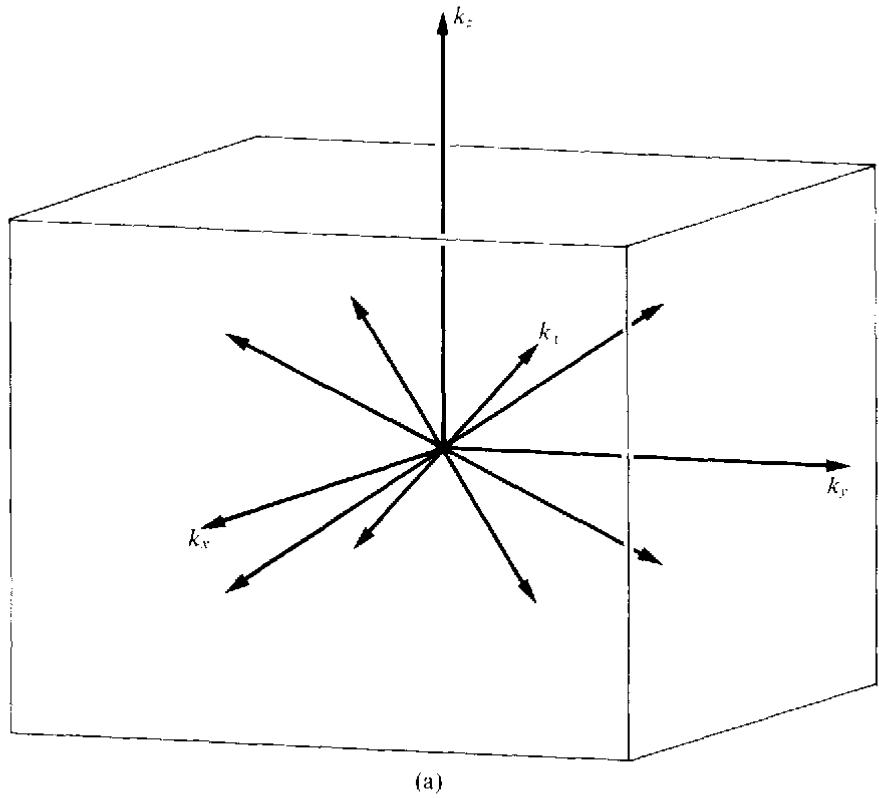
\includegraphics[width=0.75\textwidth]{fig3_19a_mu.jpg}
\caption*{\textbf{图 3.19(a)}\ 布里渊区与确定一个空间群表示的星的矢量。}
\end{figure}
\begin{figure}[H]
\centering
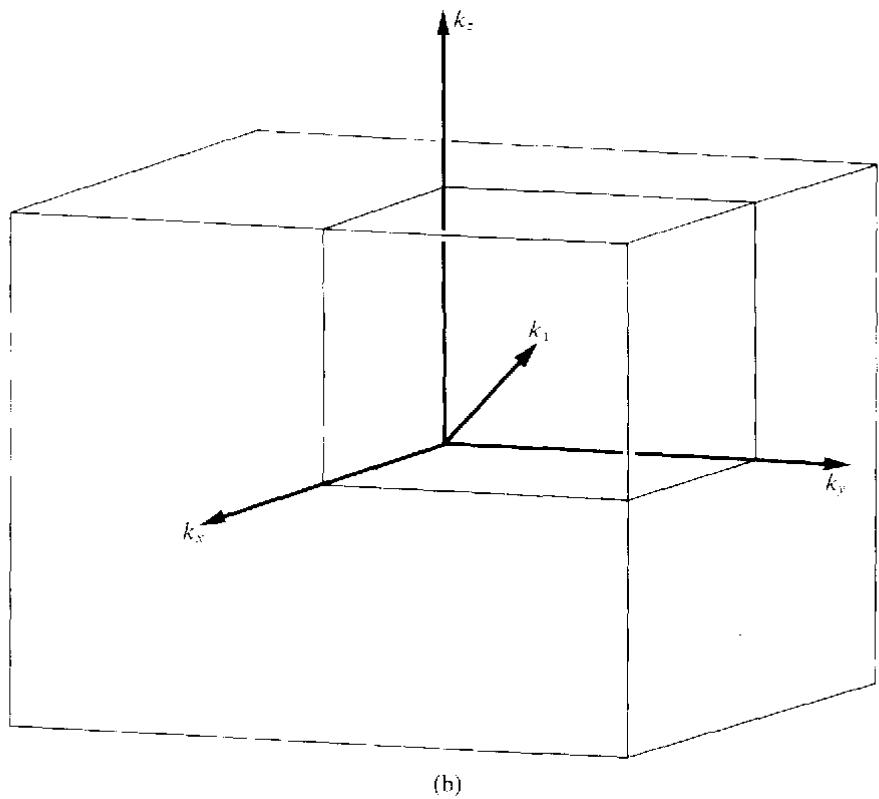
\includegraphics[width=0.75\textwidth]{fig3_19b_mu.jpg}
\caption*{\textbf{图 3.19(b)}\ 表示域与确定一个小表示的矢量。}
\end{figure}

在物理处理中人们会说：在 $\mathbf{k}_{1}$ 处有一组属于 $\Gamma^{\mathbf{k}_{1}}_{p}$ 的 $t$ 个简并本征函数（本征值 $\lambda_{1}$），并且在 $\mathbf{k}_{1}$ 的星中其他每个波矢 $S\mathbf{k}_{1}$ 处也有一组类似的 $t$ 个简并本征函数（本征值相同为 $\lambda_{1}$）。然而由于星的这些其他成员都在表示域之外，而且人们通常只关心本征值的数值（在各表示域中相同），所以只考虑 $\mathbf{k}_{1}$ 处的 $t$ 个本征函数及 $t$ 重简并的本征值。在更严格的数学处理中，则有一组 $(qt)$ 个本征函数具有本征值 $\lambda_{1}$，其中每组 $t$ 个函数与 $\mathbf{k}_{1}$ 的星中的每个波矢相联系。也就是说，$\mathbf{G}$ 的一个表示涉及 $\mathbf{k}_{1}$ 的星中的全部波矢，因此使用 $\mathbf{G}$ 的表示就要用到整个布里渊区，见图 3.19(a)。而小群 $\mathbf{G}^{\mathbf{k}_{1}}$ 的（小）表示只与表示域中的单个波矢 $\mathbf{k}_{1}$ 相联系，见图 3.19(b)。

给出了求 $\mathbf{G}$ 表示的方案之后，现在考虑它在实践中的运作。关键步骤是小表示的确定，方案的其余部分是直截了当的。这里遇到一个基本困难：群 $\mathbf{G}^{\mathbf{k}_{1}}$ 本身是一个空间群！看起来我们几乎回到了出发点。不过 $\mathbf{G}^{\mathbf{k}_{1}}$ 关于 $\mathbf{T}$ 的商群的阶 $b$ 比 $\mathbf{G}/\mathbf{T}$ 的阶 $h$ 小，因此问题有所简化。设
\begin{equation*}
\mathbf{G}^{\mathbf{k}_{1}} = \{S_{1} \mid \mathbf{w}_{1}\}\mathbf{T} + \{S_{2} \mid \mathbf{w}_{2}\}\mathbf{T} + \dots + \{S_{b} \mid \mathbf{w}_{b}\}\mathbf{T},
\tag{3.7.5}
\end{equation*}
并设
\begin{equation*}
\{S_{i} \mid \mathbf{w}_{i}\}\{S_{j} \mid \mathbf{w}_{j}\} = \{S_{i}S_{j} \mid \mathbf{w}_{i} + S_{i}\mathbf{w}_{j}\} = \{E \mid \mathbf{t}_{ij}\}\{S_{k} \mid \mathbf{w}_{k}\},
\tag{3.7.6}
\end{equation*}
其中 $\{E \mid \mathbf{t}_{ij}\} \in \mathbf{T}$，且由式 (3.7.6)
\begin{equation*}
\mathbf{t}_{ij} = \mathbf{w}_{i} + S_{i}\mathbf{w}_{j} - \mathbf{w}_{k}.
\tag{3.7.7}
\end{equation*}
因为 $\mathbf{t}_{ij}$ 是平移，所以
\begin{equation*}
\Gamma^{\mathbf{k}_{1}}_{p}\left(\{S_{i} \mid \mathbf{w}_{i}\}\right)\Gamma^{\mathbf{k}_{1}}_{p}\left(\{S_{j} \mid \mathbf{w}_{j}\}\right) = \exp\left(-\mathrm{i}\mathbf{k}_{1} \cdot (\mathbf{w}_{i} + S_{i}\mathbf{w}_{j} - \mathbf{w}_{k})\right)\Gamma^{\mathbf{k}_{1}}_{p}\left(\{S_{k} \mid \mathbf{w}_{k}\}\right).
\tag{3.7.8}
\end{equation*}
现在若对所有 $\{R \mid \mathbf{v}\} \in \mathbf{G}^{\mathbf{k}_{1}}$ 令
\begin{equation*}
\Gamma^{\mathbf{k}_{1}}_{p}(\{R \mid \mathbf{v}\}) = \exp(-\mathrm{i}\mathbf{k}_{1} \cdot \mathbf{v})\mathbf{D}^{\mathbf{k}_{1}}_{p}(\{R \mid \mathbf{v}\})
\tag{3.7.9}
\end{equation*}
则由式 (3.7.8) 得
\begin{equation*}
\mathbf{D}^{\mathbf{k}_{1}}_{p}\left(\{S_{i} \mid \mathbf{w}_{i}\}\right)\mathbf{D}^{\mathbf{k}_{1}}_{p}\left(\{S_{j} \mid \mathbf{w}_{j}\}\right) = \exp(-\mathrm{i}\mathbf{g}_{i} \cdot \mathbf{w}_{j})\mathbf{D}^{\mathbf{k}_{1}}_{p}\left(\{S_{k} \mid \mathbf{w}_{k}\}\right)
\tag{3.7.10}
\end{equation*}
其中，注意到 $S_{i}\mathbf{k}_{1} \equiv \mathbf{k}_{1}$，$\mathbf{g}_{i}$ 是由方程
\begin{equation*}
S^{-1}_{i}\mathbf{k}_{1} = \mathbf{k}_{1} + \mathbf{g}_{i}
\tag{3.7.11}
\end{equation*}
定义的倒格子矢量。另外，若 $\{E \mid \mathbf{t}\} \in \mathbf{T}$，则由式 (3.7.9)
\begin{equation*}
\mathbf{D}^{\mathbf{k}_{1}}_{p}(\{E \mid \mathbf{t}\}) = 1.
\tag{3.7.12}
\end{equation*}
同样正确的是：若 $\{E \mid \mathbf{t}\} \in \mathbf{T}$，则
\begin{equation*}
\exp\left\{-\mathrm{i}\mathbf{g}_{i} \cdot (\mathbf{w}_{j} + \mathbf{t})\right\} = \exp(-\mathrm{i}\mathbf{g}_{i} \cdot \mathbf{w}_{j}).
\tag{3.7.13}
\end{equation*}
式 (3.7.12)、(3.7.13) 与 (3.7.10) 合起来意味着：$\mathbf{D}^{\mathbf{k}_{1}}_{p}$ 的矩阵对式 (3.7.5) 中任一固定陪集的所有成员都是相同的。也就是说，$\mathbf{D}^{\mathbf{k}_{1}}_{p}$ 是定义在商群 $\mathbf{G}^{\mathbf{k}_{1}}/\mathbf{T}$ 的元素上的矩阵值函数。但这个商群同构于小陪群 $\overline{\mathbf{G}}^{\mathbf{k}_{1}}$。

因此可以把式 (3.7.10) 改写为
\begin{equation*}
\mathbf{D}^{\mathbf{k}_{1}}_{p}(S_{i})\mathbf{D}^{\mathbf{k}_{1}}_{p}(S_{j}) = \exp(-\mathrm{i}\mathbf{g}_{i} \cdot \mathbf{w}_{j})\mathbf{D}^{\mathbf{k}_{1}}_{p}(S_{k}),
\tag{3.7.14}
\end{equation*}
其中 $S_{i}S_{j} = S_{k}$ 且 $S^{-1}_{i}\mathbf{k}_{1} = \mathbf{k}_{1} + \mathbf{g}_{i}$。

由式 (3.7.14) 可见，在如下两种重要情形中 $\mathbf{D}^{\mathbf{k}_{1}}_{p}$ 是 $\overline{\mathbf{G}}^{\mathbf{k}_{1}}$ 到一组矩阵的同态：

（i）若对所有 $j = 1$ 到 $b$ 有 $\mathbf{w}_{j} = 0$。这是空间群 $\mathbf{G}$ 为点式群的情形。

（ii）若对所有 $i = 1$ 到 $b$ 有 $S^{-1}_{i}\mathbf{k}_{1} = \mathbf{k}_{1}$（即 $\mathbf{g}_{i} = 0$）。这是 $\mathbf{k}_{1}$ 为布里渊区内点的情形，因为此时布里渊区中与 $\mathbf{k}_{1}$ 等价的点只有 $\mathbf{k}_{1}$ 自己。

当 $\mathbf{D}^{\mathbf{k}_{1}}_{p}$ 是同态时，它是小陪群的一个表示，而且 $\Gamma^{\mathbf{k}_{1}}_{p}$ 的不可约性意味着 $\mathbf{D}^{\mathbf{k}_{1}}_{p}$ 也必不可约。因此在上述两种情形中，我们要做的只是求出小陪群 $\overline{\mathbf{G}}^{\mathbf{k}_{1}}$ 的不可约表示——这可以从表 2.2 与 2.3 读出。

剩下的唯一情形是 $\mathbf{k}_{1}$ 位于布里渊区面上而空间群为非点式群的情形。

若 $\mathbf{k}_{1}$ 是一般点，则小陪群仅由恒等元构成，又回到情形 (ii)。于是仅有的困难情形是：非点式空间群且 $\mathbf{k}_{1}$ 是对称点，或者 $\mathbf{k}_{1}$ 位于布里渊区面上的对称线或对称面上。

为了覆盖这些困难情形，需要引入有限群的\textit{射影表示}（projective representation）概念。

\noindent\textbf{定义 3.7.5}\quad （射影表示）\ 定义在群 $\mathbf{H}$（由元素 $H_{i}$，$i = 1$ 到 $|\mathbf{H}|$ 组成）上的非奇异矩阵值函数 $\Delta$ 称为 $\mathbf{H}$ 的射影表示，若它满足如下规则：

若对每个群乘积 $H_{i}H_{j} = H_{k}$，存在有序对 $H_{i}, H_{j}$ 上的标量函数 $\mu(H_{i}, H_{j})$ 使得
\begin{equation*}
\Delta(H_{i})\Delta(H_{j}) = \mu(H_{i}, H_{j})\Delta(H_{k})
\tag{3.7.15}
\end{equation*}
并且对一切 $i, j, l$ 有
\begin{equation*}
\mu(H_{i}, H_{j}H_{l})\mu(H_{j}, H_{l}) = \mu(H_{i}H_{j}, H_{l})\mu(H_{i}, H_{j}),
\tag{3.7.16}
\end{equation*}
则称 $\Delta$ 为 $\mathbf{H}$ 的射影表示。式 (3.7.16) 是矩阵乘法结合律的要求。

函数 $\mu(H_{i}, H_{j})$ 构成所谓的射影表示 $\Delta$ 的\textit{因子系统}（factor system）。若对所有 $i, j$ 有 $\mu(H_{i}, H_{j}) = 1$，则射影表示 $\Delta$ 成为普通（矢量）表示。若对所有 $i, j$ 有 $|\mu(H_{i}, H_{j})| = 1$，则总可以施行一个变换使 $\Delta$ 幺正化。幺正射影表示满足与式 (1.3.11) 类似的正交关系：
\begin{equation*}
\sum^{|H|}_{j=1}\Delta^{i}(H_{j})^{*}_{pv}\Delta^{k}(H_{j})_{qw} = \frac{|\mathbf{H}|}{d_{i}}\delta^{ik}\delta_{pq}\delta_{vw},
\tag{3.7.17}
\end{equation*}
相应地，对特征标有
\begin{equation*}
\sum^{|H|}_{j=1}\chi^{i*}(H_{j})\chi^{k}(H_{j}) = |\mathbf{H}|\delta^{ik}.
\tag{3.7.18}
\end{equation*}
给定带因子系统 $\mu$ 的射影表示 $\Delta$，若令
\begin{equation*}
\Delta'(H_{i}) = C_{i}\Delta(H_{i}) \quad\text{对一切 } i,
\tag{3.7.19}
\end{equation*}
其中 $C_{i}$ 是复数，则与式 (3.7.15) 相应的方程为
\begin{equation*}
\Delta'(H_{i})\Delta'(H_{j}) = \frac{C_{i}C_{j}}{C_{k}}\mu(H_{i}, H_{j})\Delta'(H_{k}).
\tag{3.7.20}
\end{equation*}
若再写
\begin{equation*}
\nu(H_{i}, H_{j}) = \frac{C_{i}C_{j}}{C_{k}}\mu(H_{i}, H_{j})
\tag{3.7.21}
\end{equation*}
则 $\Delta'$ 是 $\mathbf{H}$ 的带因子系统 $\nu$ 的射影表示。凡由形如 (3.7.21) 的方程相联系的两个因子系统称为属于同一个\textit{类}。由于关系 (3.7.19) 很简单，我们只需从每个类中选一个因子系统来研究。为从特定类中选取合适的因子系统，注意到
\begin{equation*}
\Delta(E) = \mu(E, E)\mathbf{1}
\tag{3.7.22}
\end{equation*}
若对所有 $i$ 令 $\Delta'(H_{i}) = \Delta(H_{i})/\mu(E, E)$，则
\begin{equation*}
\Delta'(E) = 1.
\tag{3.7.23}
\end{equation*}
再由式 (3.7.21) 定义新的因子系统 $\nu$，取 $1/C_{i} = \mu(E, E)$ 对一切 $i$ 成立，则因为
\begin{equation*}
\Delta'(H_{i})\Delta'(E) = \nu(H_{i}, E)\Delta'(H_{i})
\end{equation*}
必须有
\begin{equation*}
\nu(H_{i}, E) = 1 \quad\text{对一切 } H_{i}.
\tag{3.7.24}
\end{equation*}
类似地
\begin{equation*}
\nu(E, H_{i}) = 1 \quad\text{对一切 } H_{i}.
\tag{3.7.25}
\end{equation*}
（对任何因子系统 $\mu$，当然有 $\mu(H_{i}, E) = \mu(E, H_{i}) = \mu(E, E)$，以及 $\mu(H_{i}, H^{-1}_{i}) = \mu(H^{-1}_{i}, H_{i})$。）

现在不加证明地引用 Schur 关于射影表示的若干定理。

\noindent\textbf{定理 3.7.1}\quad 有限群 $\mathbf{H}$ 的因子系统的类数 $m$ 是有限的；这些类可以与一个 $m$ 阶 Abel 群 $\mathbf{M}$（称为 $\mathbf{H}$ 的\textit{乘子}（multiplier））的元素一一对应。

这一对应是这样的：若把 $\mathbf{M}$ 的元素记为 $M_{1}, M_{2}, \dots, M_{m}$，而 $\mu_{p}$、$\mu_{q}$ 是从分别对应于 $M_{p}$ 与 $M_{q}$ 的类中任取的因子系统，则对一切 $i, j$ 由
\begin{equation*}
\mu_{r}(H_{i}, H_{j}) = \mu_{p}(H_{i}, H_{j})\mu_{q}(H_{i}, H_{j})
\tag{3.7.26}
\end{equation*}
定义的因子系统 $\mu_{r}$ 总属于对应于 $M_{r}$ 的类，其中 $M_{r} = M_{p}M_{q}$。此外，$\mathbf{M}$ 的每个元素的阶都整除 $|\mathbf{H}|$。特别地，若 $M_{p}$ 的阶为 $\alpha_{p}$，则可以从对应于 $M_{p}$ 的类中选出一个代表因子系统，其取值全是单位根的 $\alpha_{p}$ 次幂。

Schur 的理论进而证明：对每个 $|\mathbf{H}|$ 阶、乘子 $\mathbf{M}$ 为 $m$ 阶的有限群 $\mathbf{H}$，可以构造一个 $|\mathbf{H}|m$ 阶的群 $\mathbf{H}_{M}$，使 $\mathbf{M}$ 同构于 $\mathbf{H}_{M}$ 中心的一个子群（群的中心是与所有元素可交换的不变子群）。

\noindent\textbf{定理 3.7.2}\quad 通过遍取 $\mathbf{H}_{M}$ 的所有表示并限制在 $\mathbf{H}$ 的元素上，可以（在等价意义下）得到 $\mathbf{H}$ 的全部可能的幺正不可约射影表示。

联系这个定理必须意识到：尽管 $\mathbf{H}$ 的元素可以被认作 $\mathbf{H}_{M}/\mathbf{M}$ 的陪集代表，$\mathbf{H}_{M}$ 的构造方式使得除平凡情形 $m = 1$ 外，$\mathbf{H}_{M}$ 中被认定为 $\mathbf{H}$ 元素的那些元素的乘法规则与 $\mathbf{H}$ 中的乘法规则不同。

由于这个定理比我们需要的更强，我们将不说明如何构造 $\mathbf{H}_{M}$。记住我们只要求属于给定因子系统的射影表示。我们将不构造 $\mathbf{H}_{M}$，而是说明如何构造另一个群 $\mathbf{H}^{*}$，它给出的是属于给定因子系统的全部不可约射影表示（而不是所有因子系统的）。

设我们有一个群 $\mathbf{H}$，希望求出它属于给定因子系统 $\mu$ 的幺正不可约射影表示。由目前的讨论可知，可以把 $\mu$ 选成对一切 $j, k$ 有
\begin{equation*}
\mu(H_{j}, H_{k}) = \exp\left\{2\pi\mathrm{i}\,a(H_{j}, H_{k})/g\right\},
\tag{3.7.27}
\end{equation*}
其中 $g$ 与 $a(H_{j}, H_{k})$ 是由已知的 $\mu(H_{j}, H_{k})$ 及条件 $0 \leqslant a(H_{j}, H_{k}) \leqslant g-1$ 确定的整数，并且（见式 (3.7.24) 与 (3.7.25)）
\begin{equation*}
a(H_{j}, E) = a(E, H_{j}) = 0.
\tag{3.7.28}
\end{equation*}
另外，由于 $\mu(H_{j}, H^{-1}_{j}) = \mu(H^{-1}_{j}, H_{j})$，
\begin{equation*}
a(H_{j}, H^{-1}_{j}) = a(H^{-1}_{j}, H_{j})
\tag{3.7.29}
\end{equation*}
且由式 (3.7.16) 与 (3.7.27)，
\begin{equation*}
a(H_{i}, H_{j}H_{l}) + a(H_{j}, H_{l}) = a(H_{i}H_{j}, H_{l}) + a(H_{i}, H_{j}), \mod g.
\tag{3.7.30}
\end{equation*}
设 $\mathbf{Z}_{g}$ 是整数 $0, 1, \dots, (g-1)$ 的循环群，群乘法定义为模 $g$ 加法。

设 $\mathbf{H}^{*}$ 由 $g|\mathbf{H}|$ 个元素（即一对一对的 $(H_{j}, \alpha)$，其一来自 $\mathbf{H}$，另一来自 $\mathbf{Z}_{g}$）组成，并用方程
\begin{equation*}
(H_{j}, \alpha)(H_{k}, \beta) = (H_{j}H_{k}, \alpha + \beta + a(H_{j}, H_{k}))
\tag{3.7.31}
\end{equation*}
定义乘法规则。关于这一乘法规则 $\mathbf{H}^{*}$ 是群：封闭性显然；结合性由 $\mathbf{H}$ 与 $\mathbf{Z}_{g}$ 中的结合性及式 (3.7.30) 得到；$\mathbf{H}^{*}$ 的恒等元是 $(E, 0)$；$(H_{j}, \alpha)$ 的逆是 $(H^{-1}_{j}, -\alpha - a(H^{-1}_{j}, H_{j}))$。

由式 (3.7.31) 与 (3.7.28) 可知，对一切 $\alpha, \beta, k$ 有
\begin{equation*}
(E, \alpha)(H_{k}, \beta) = (H_{k}, \beta)(E, \alpha) = (H_{k}, \alpha + \beta).
\tag{3.7.32}
\end{equation*}
式 (3.7.32) 蕴含由 $g$ 个元素 $(E, \alpha)$ 组成的子群位于 $\mathbf{H}^{*}$ 的中心。既然 $(E, \alpha)$ 与 $\mathbf{H}^{*}$ 的所有元素可交换，由 Schur 引理（见定理 1.3.6）可知，若 $\Gamma$ 是 $\mathbf{H}^{*}$ 的表示，则 $\Gamma(E, \alpha)$ 是单位矩阵的标量倍。

现在假设存在 $\mathbf{H}^{*}$ 的一个表示使得对一切 $\alpha \in \mathbf{Z}_{g}$ 有
\begin{equation*}
\Gamma(E, \alpha) = \exp(2\pi\mathrm{i}\alpha/g)\mathbf{1}.
\tag{3.7.33}
\end{equation*}
则
\begin{equation*}
\Gamma(H_{k}, \beta) = \Gamma(H_{k}, 0)\Gamma(E, \beta) = \Gamma(H_{k}, 0)\exp(2\pi\mathrm{i}\beta/g)
\tag{3.7.34}
\end{equation*}
记 $\Gamma(H_{k}, 0) = \Delta(H_{k})$，便有
\begin{equation*}
\begin{aligned}
\Delta(H_{j})\Delta(H_{k}) &= \Gamma(H_{j}, \alpha)\Gamma(H_{k}, \beta)\exp\left\{-2\pi\mathrm{i}(\alpha + \beta)/g\right\}\\
&= \Gamma(H_{j}H_{k}, \alpha + \beta + a(H_{j}, H_{k}))\exp\left\{-2\pi\mathrm{i}(\alpha + \beta)/g\right\}\\
&= \Delta(H_{j}H_{k})\exp\left\{2\pi\mathrm{i}\,a(H_{j}, H_{k})/g\right\}.
\end{aligned}
\tag{3.7.35}
\end{equation*}
由式 (3.7.35) 与 (3.7.27) 可知 $\Delta$ 是 $\mathbf{H}$ 的带因子系统 $\mu$ 的射影表示。而且它是幺正的（因为 $\Gamma$ 幺正），也是不可约的（因为若 $\Delta$ 可约，则由于 $(E, \alpha)$ 对一切 $\alpha$ 由标量矩阵表示，$\Gamma$ 的所有矩阵就都与 $\Delta$ 的矩阵处于同样的分块对角形式，与 $\Gamma$ 的不可约性矛盾）。

反之，若 $\Delta$ 是 $\mathbf{H}$ 的幺正不可约射影表示，且对一切 $k, \beta$ 令
\begin{equation*}
\Gamma(H_{k}, \beta) = \Delta(H_{k})\exp(2\pi\mathrm{i}\beta/g)
\tag{3.7.36}
\end{equation*}
则 $\Gamma$ 是 $\mathbf{H}^{*}$ 的表示。于是用纯数学家的语言说，$\mathbf{H}$ 的全部不可约射影表示都可以提升到 $\mathbf{H}^{*}$ 中，也就是说可以由 $\mathbf{H}^{*}$ 的普通矢量表示求得。

现在回到小陪群，考察我们关心的因子系统。把 $\overline{\mathbf{G}}^{\mathbf{k}_{1}}$ 认同于 $\mathbf{H}$，把 $\mathbf{D}^{\mathbf{k}_{1}}_{p}$ 认同于 $\Delta$。因子系统由下式给出：
\begin{equation*}
\mu(S_{i}, S_{j}) = \exp(-\mathrm{i}\mathbf{g}_{i} \cdot \mathbf{w}_{j})
\tag{3.7.37}
\end{equation*}
其中
\begin{equation*}
S^{-1}_{i}\mathbf{k}_{1} = \mathbf{k}_{1} + \mathbf{g}_{i}
\tag{3.7.11}
\end{equation*}
而 $\mathbf{w}_{j}$ 是在 $\mathbf{G}^{\mathbf{k}_{1}}$ 关于 $\mathbf{T}$ 的左陪集分解 (3.7.5) 中与 $S_{j}$ 相联系的平移部分。

由式 (3.7.11) 可见，当 $S_{i} = E$ 时 $\mathbf{g}_{i} = 0$，故
\begin{equation*}
\mu(E, S_{j}) = 1 \quad\text{对一切 } j.
\end{equation*}
此外，由于 $\mathbf{w}_{j}$ 总是平移的分数部分，$\mu(S_{j}, S_{k})$ 总具有 (3.7.27) 的形式；更重要的是，$g$ 必然是个小数目（事实上是 2、3、4 或 6）。于是由式 (3.7.37) 定义的因子系统已经处于适于上述处理的形式。这意味着，为求出空间群的所有表示，只需找出几个小群（的中央延拓群）的普通表示就够了。

作为本节的最后一点，通过分析 $\mathbf{H}_{M}$ 的表示的维数，并注意其中哪些对给定因子系统成为不可约幺正射影表示，可以证明一个与定理 1.3.11 类似的定理：若给定因子系统的射影表示的维数为 $d_{i}$，则 $\sum_{i}d^{2}_{i} = |\mathbf{H}|$。这使式 (3.7.17) 可以反过来产生另一个矩阵元的正交关系。但要注意，$i$ 的取值个数不一定等于 $\mathbf{H}$ 的类的数目（这与普通矢量表示不同）。

% 3.8 例子：立方密堆积与金刚石结构
\section{例子：立方密堆积与金刚石结构}

本节给出两个例子来说明前几节的理论；一个是点式空间群——立方密堆积 $Fm3m\ (O^{5}_{h})$，另一个是非点式空间群——金刚石结构的空间群 $Fd3m\ (O^{7}_{h})$。这两个空间群分别最先由 Bouckaert, Smoluchowski, and Wigner (1936) 与 Herring (1942) 处理过。

二者都建立在面心立方（$F$）布拉维格子 $\Gamma^{f}_{c}$ 上，故由表 3.1，两种情形的格子平移都是
\begin{equation*}
\left\{
\begin{array}{l}
\mathbf{t}_{1} = \frac{1}{2}(0, a, a),\\
\mathbf{t}_{2} = \frac{1}{2}(a, 0, a),\\
\mathbf{t}_{3} = \frac{1}{2}(a, a, 0).
\end{array}
\right.
\tag{3.8.1}
\end{equation*}
两种情形的同形点群 $\mathbf{F}$ 都是 $m3m\ (O_{h})$，即完整立方群。

由表 3.3 可见倒格子矢量为
\begin{equation*}
\left\{
\begin{array}{l}
\mathbf{g}_{1} = (2\pi/a)(-1, 1, 1),\\
\mathbf{g}_{2} = (2\pi/a)(1, -1, 1),\\
\mathbf{g}_{3} = (2\pi/a)(1, 1, -1),
\end{array}
\right.
\tag{3.8.2}
\end{equation*}
布里渊区示于图 3.14。

由表 3.7 可见，对 $Fm3m\ (O^{5}_{h})$，$m3m\ (O_{h})$ 的每个转动算符都只与纯格子平移相联系，于是关于平移群 $\mathbf{T}$ 的一个合适的左陪集分解为
\begin{equation*}
Fm3m\left(O^{5}_{h}\right) = \sum_{R}\{R \mid 000\}\mathbf{T}
\tag{3.8.3}
\end{equation*}
其中对 $R$ 的求和取遍 $m3m\ (O_{h})$ 的所有元素。而对 $Fd3m\ (O^{7}_{h})$，只有属于子群 $\bar{4}3m\ (T_{d})$ 的算符与纯格子平移相联系，相应的左陪集分解为
\begin{equation*}
Fd3m\left(O^{7}_{h}\right) = \sum_{R}\{R \mid 000\}\mathbf{T} + \sum_{R}\{RI \mid {\textstyle\frac{1}{4}}{\textstyle\frac{1}{4}}{\textstyle\frac{1}{4}}\}\mathbf{T}
\tag{3.8.4}
\end{equation*}
此时对 $R$ 的求和取遍 $\bar{4}3m\ (T_{d})$ 的所有元素，且如通常，$I$ 是反演。与不在 $\bar{4}3m\ (T_{d})$ 中的 $m3m\ (O_{h})$ 元素相对应的那些陪集，其陪集代表总可取为 $\mathbf{v} = \frac{1}{4}(\mathbf{t}_{1} + \mathbf{t}_{2} + \mathbf{t}_{3}) = \frac{1}{4}(a, a, a)$（在 $Oxyz$ 轴下）。算符 $R$ 作用在（$Oxyz$ 轴下的）非零平移 $(p, q, r)$ 上的效果可由表 1.4 查出，例如 $C^{-}_{4z}(p, q, r) = (q, -p, r)$。算符 $R$ 作用在布拉维格子基本矢量 $\mathbf{t}_{1}$、$\mathbf{t}_{2}$、$\mathbf{t}_{3}$ 上的效果可由表 3.2 查出，例如对立方 $F$ 格子 $C^{-}_{4z}\mathbf{t}_{1} = \mathbf{t}_{2}$、$C^{-}_{4z}\mathbf{t}_{2} = \mathbf{t}_{2} - \mathbf{t}_{3}$、$C^{-}_{4z}\mathbf{t}_{3} = -\mathbf{t}_{1} + \mathbf{t}_{2}$。

在表 3.11 中我们列出了布里渊区基本域中我们求 $Fm3m\ (O^{5}_{h})$ 与 $Fd3m\ (O^{7}_{h})$ 的表示时所需要的对称点、对称线和对称面以及一个一般点。它们就是 3.7 节的点 $\mathbf{k}_{1}$。两种情形下，由于 $\mathbf{F}$ 是布拉维格子的全对称点群，表示域与基本域重合，因此就是图 3.14 所示的区域。

\begin{figure}[H]
\centering
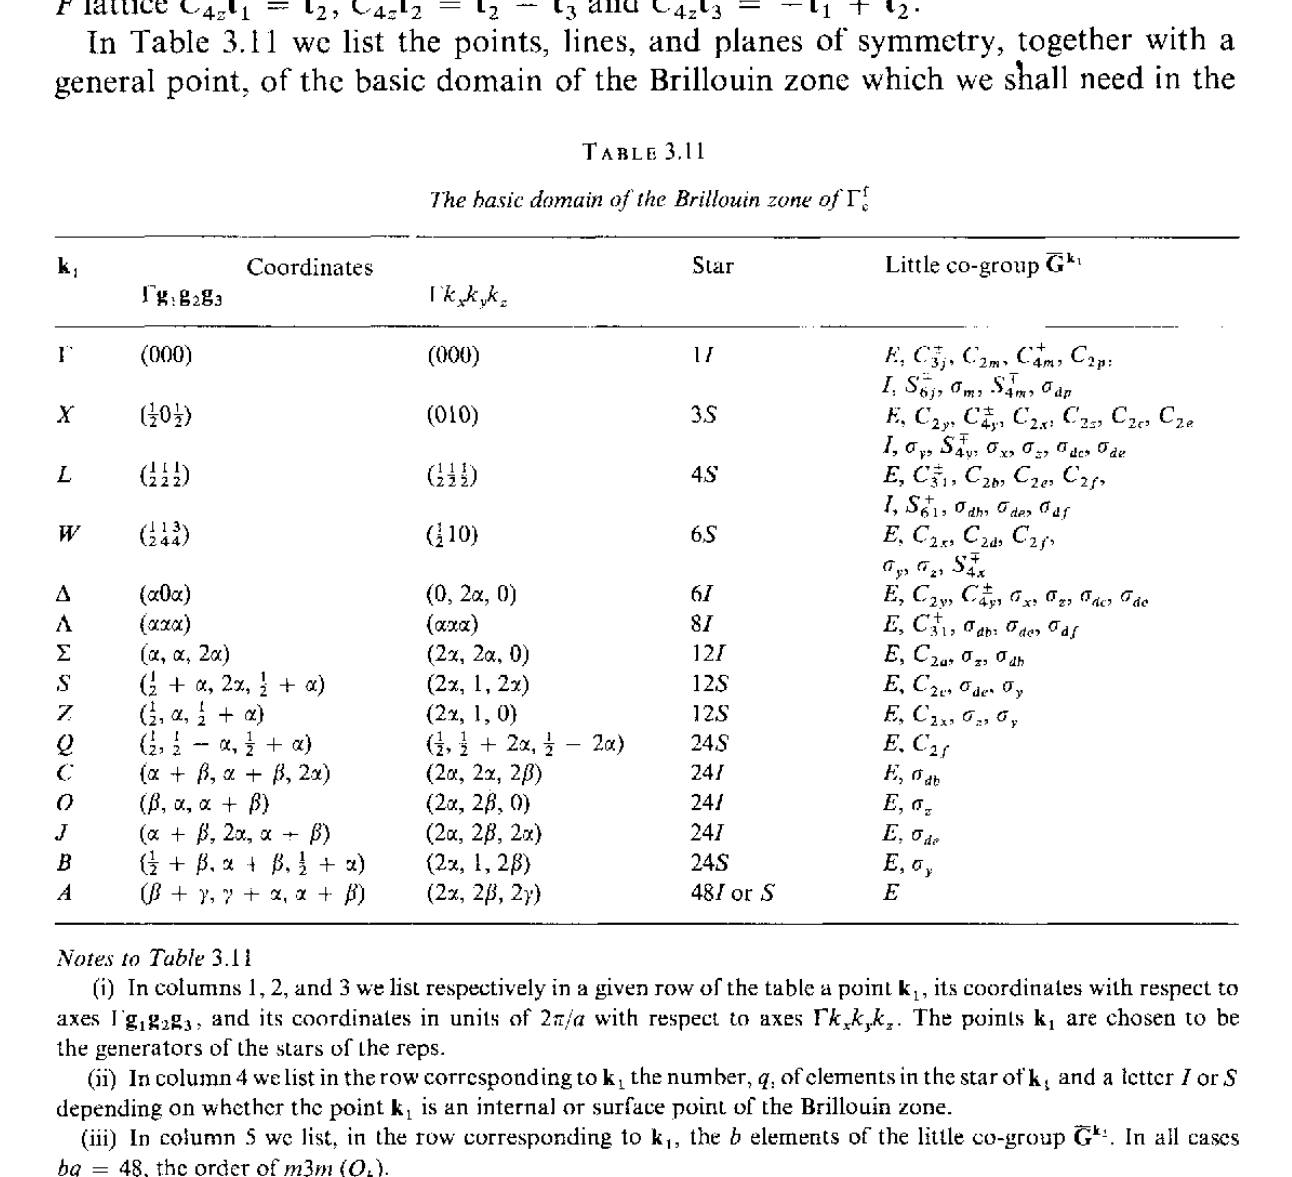
\includegraphics[width=0.88\textwidth]{c3_t311.png}
\caption*{\textbf{表 3.11}\ $\Gamma^{f}_{c}$ 的布里渊区的基本域（原书扫描占位）。}
\end{figure}

表 3.11 的注（译文）：

\noindent（i）第 1、2、3 列在表的每一行中分别列出点 $\mathbf{k}_{1}$、它相对于轴 $\Gamma\mathbf{g}_{1}\mathbf{g}_{2}\mathbf{g}_{3}$ 的坐标，以及它以 $2\pi/a$ 为单位、相对于轴 $\Gamma k_{x}k_{y}k_{z}$ 的坐标。点 $\mathbf{k}_{1}$ 选为表示的星的生成元。

\noindent（ii）第 4 列在对应于 $\mathbf{k}_{1}$ 的行中列出 $\mathbf{k}_{1}$ 的星中元素的数目 $q$，以及字母 I 或 S——视 $\mathbf{k}_{1}$ 是布里渊区的内部点还是表面点而定。

\noindent（iii）第 5 列在对应于 $\mathbf{k}_{1}$ 的行中列出小陪群 $\overline{\mathbf{G}}^{\mathbf{k}_{1}}$ 的 $b$ 个元素。所有情形都有 $bq = 48$，即 $m3m\ (O_{h})$ 的阶。

\noindent（iv）本表对两个空间群乃至一切基于 $\Gamma^{f}_{c}$ 且同形点群为 $m3m\ (O_{h})$ 的空间群都是共同的；另见表 3.6 的相应部分。表 3.11 中有而表 3.6 中没有的点，是对称面上的点与一般点。除本例外我们将不再列出对称面，因为如我们将看到的，它们很容易处理。

现在考虑把小群 $\mathbf{G}^{\mathbf{k}_{1}}$ 关于平移群 $\mathbf{T}$ 作左陪集分解。对 $Fm3m$ 有
\begin{equation*}
\mathbf{G}^{\mathbf{k}_{1}} = \sum_{S}\{S \mid 000\}\mathbf{T}
\tag{3.8.5}
\end{equation*}
其中对 $S$ 的求和取遍 $\overline{\mathbf{G}}^{\mathbf{k}_{1}}$ 的所有元素（这些群见表 3.11）。而对 $Fd3m$ 有
\begin{equation*}
\mathbf{G}^{\mathbf{k}_{1}} = \sum_{P}\{P \mid 000\}\mathbf{T} + \sum_{Q}\{Q \mid {\textstyle\frac{1}{4}}{\textstyle\frac{1}{4}}{\textstyle\frac{1}{4}}\}\mathbf{T},
\tag{3.8.6}
\end{equation*}
其中对 $P$ 的求和取遍 $\overline{\mathbf{G}}^{\mathbf{k}_{1}}$ 与 $\bar{4}3m\ (T_{d})$ 共有的元素，对 $Q$ 的求和取遍 $\overline{\mathbf{G}}^{\mathbf{k}_{1}}$ 的其余元素。

\subsection*{Fm3m}

$Fm3m$ 可以很快处理完。给定任一点 $\mathbf{k}_{1}$，需要确定 $\overline{\mathbf{G}}^{\mathbf{k}_{1}}$ 带因子系统 $\exp(-\mathrm{i}\mathbf{g}_{i} \cdot \mathbf{w}_{j})$ 的射影表示，其中 $\mathbf{g}_{i}$ 由式 (3.7.11) 给出，$\mathbf{w}_{j}$ 是分解 (3.8.5) 中与 $S_{j}$ 相联系的平移。立即看出对所有 $j$ 有 $\mathbf{w}_{j} = 0$。因此因子系统完全由单位元组成，属于 $\overline{\mathbf{G}}^{\mathbf{k}_{1}}$ 的乘子的恒等元所对应的类。于是合适的表示 $\mathbf{D}^{\mathbf{k}_{1}}_{p}$ 就是 $\overline{\mathbf{G}}^{\mathbf{k}_{1}}$ 的普通矢量表示；而且由于 $\overline{\mathbf{G}}^{\mathbf{k}_{1}}$ 是点群（诚然某些情形下定向非标准），可以从表 2.2 得到 $\mathbf{D}^{\mathbf{k}_{1}}_{p}$。

$\mathbf{G}^{\mathbf{k}_{1}}$ 的小表示 $\Gamma^{\mathbf{k}_{1}}_{p}$ 现在由式 (3.7.9) 立即得到。$\Gamma^{\mathbf{k}_{1}}_{p}$ 的矩阵在所有情形都与 $\mathbf{D}^{\mathbf{k}_{1}}_{p}$ 的矩阵通过方程
\begin{equation*}
\Gamma^{\mathbf{k}_{1}}_{p}(\{S \mid \mathbf{t}\}) = \exp(-\mathrm{i}\mathbf{k}_{1} \cdot \mathbf{t})\mathbf{D}^{\mathbf{k}_{1}}_{p}(S)
\tag{3.8.7}
\end{equation*}
相联系。因此只需指明点群 $\overline{\mathbf{G}}^{\mathbf{k}_{1}}$ 即可把 $Fm3m$ 处理完毕。结果如下：对 $\Gamma$，$m3m\ (O_{h})$；对 $X$，$4/mmm\ (D_{4h})$；对 $L$，$\bar{3}m\ (D_{3d})$；对 $W$，$\bar{4}2m\ (D_{2d})$；对 $\Delta$，$4mm\ (C_{4v})$；对 $\Lambda$，$3m\ (C_{3v})$；对 $\Sigma$，$mm2\ (C_{2v})$；对 $S$，$mm2\ (C_{2v})$；对 $Z$，$mm2\ (C_{2v})$；对 $Q$，$2\ (C_{2})$；对 $C$，$m\ (C_{1h})$；对 $O$，$m\ (C_{1h})$；对 $J$，$m\ (C_{1h})$；对 $B$，$m\ (C_{1h})$；对 $A$，$1\ (C_{1})$。

\subsection*{Fd3m}

金刚石的情形就不那么容易了。首先注意到，在分解 (3.8.6) 中，若陪集代表的转动部分 $P$ 是元素 $E$、$C^{\pm}_{3j}$、$C_{2m}$、$\sigma_{dp}$ 或 $S^{\pm}_{4m}$ 之一，则其平移部分 $\mathbf{w}_{j} = 0$；而若其转动部分 $Q$ 是元素 $I$、$S^{\mp}_{6j}$、$\sigma_{m}$、$C_{2p}$ 或 $C^{\pm}_{4m}$ 之一，则其平移部分 $\mathbf{w}_{j} = \mathbf{v} = \frac{1}{4}(a, a, a)$。因此因子系统 $\exp(-\mathrm{i}\mathbf{g}_{i} \cdot \mathbf{w}_{j})$ 在下述两种情形完全由单位元组成：对所有 $i$ 有 $\mathbf{g}_{i} = \mathbf{0}$；或者小陪群 $\overline{\mathbf{G}}^{\mathbf{k}_{1}}$ 的元素全部形如 $P$ 而没有形如 $Q$ 的元素。前者在 $\mathbf{k}_{1}$ 是布里渊区内点时成立（$\Gamma, \Delta, \Lambda, \Sigma, C, O, J, A(\mathrm{I})$），后者在 $\overline{\mathbf{G}}^{\mathbf{k}_{1}}$ 完全由 $\bar{4}3m\ (T_{d})$ 中的元素组成时成立（$\Lambda, C, J, A(\mathrm{S})$）。这些情形所需的射影表示 $\mathbf{D}^{\mathbf{k}_{1}}_{p}$ 就是点群 $\overline{\mathbf{G}}^{\mathbf{k}_{1}}$ 的普通表示。

于是，在 $Fd3m$ 中若 $\mathbf{k}_{1} = \Gamma, \Delta, \Lambda, \Sigma, C, O, J$ 或 $A$，求 $\mathbf{D}^{\mathbf{k}_{1}}_{p}$ 时只需在表 2.2 中查 $\overline{\mathbf{G}}^{\mathbf{k}_{1}}$ 的表示即可。与这些点对应的点群 $\overline{\mathbf{G}}^{\mathbf{k}_{1}}$ 的名称已在上面处理 $Fm3m$ 时给出。然而，即使对这些点，$Fd3m$ 与 $Fm3m$ 之间也有本质差别：得到 $\mathbf{D}^{\mathbf{k}_{1}}_{p}$ 之后，小表示 $\Gamma^{\mathbf{k}_{1}}_{p}$ 的导出方式与 $Fm3m$ 不完全一样。此时由式 (3.7.9) 可见
\begin{equation*}
\Gamma^{\mathbf{k}_{1}}_{p}(\{P \mid \mathbf{t}\}) = \exp(-\mathrm{i}\mathbf{k}_{1} \cdot \mathbf{t})\mathbf{D}^{\mathbf{k}_{1}}_{p}(P),
\tag{3.8.8}
\end{equation*}
但
\begin{equation*}
\Gamma^{\mathbf{k}_{1}}_{p}(\{Q \mid \mathbf{t} + \mathbf{v}\}) = \exp\left(-\mathrm{i}\mathbf{k}_{1} \cdot (\mathbf{t} + \mathbf{v})\right)\mathbf{D}^{\mathbf{k}_{1}}_{p}(Q),
\tag{3.8.9}
\end{equation*}
其中 $P$ 与 $Q$ 的含义与分解 (3.8.6) 中相同。由于习惯上列出的是小表示 $\Gamma^{\mathbf{k}_{1}}_{p}$ 而非 $\mathbf{D}^{\mathbf{k}_{1}}_{p}$，表中出现的某些元素带有一个额外因子 $\exp(-\mathrm{i}\mathbf{k}_{1} \cdot \mathbf{v})$，它不出现在相应点群的特征标表中。（值得指出，对 $\Gamma$ 这个因子总是 1，因此属于 $\Gamma$ 的非点式空间群的表示与相应点式空间群的表示相同。）

现在详细考虑布里渊区的每个表面点 $B, Q, Z, S, L, W$ 和 $X$。我们将不加解释地使用 3.7 节后面各段的记号。

\subsection*{B}

$\mathbf{G}^{B}$ 的陪集代表：$\{E \mid 000\}$，$\{\sigma_{y} \mid {\frac{1}{4}}{\frac{1}{4}}{\frac{1}{4}}\}$。

\begin{center}
$EB = B$，于是 $\mathbf{g}_{E} = 0$。

$\sigma_{y}B = B - \mathbf{g}_{1} - \mathbf{g}_{3}$，于是 $\mathbf{g}_{\sigma_{y}} = -\mathbf{g}_{1} - \mathbf{g}_{3} = (-1, 0, -1)$。
\end{center}

因子系统：$\mu(E, E) = 1$，$\mu(E, \sigma_{y}) = 1$，$\mu(\sigma_{y}, E) = 1$，以及 $\mu(\sigma_{y}, \sigma_{y}) = \exp\left(2\pi\mathrm{i}\left(\frac{1}{4} + 0 + \frac{1}{4}\right)\right) = -1$。

中央延拓群 $\overline{\mathbf{G}}^{B*}$ 由四个元素 $(E, 0)$、$(E, 1)$、$(\sigma_{y}, 0)$、$(\sigma_{y}, 1)$ 组成，乘法表为
\begin{center}
\begin{tabular}{lcccc}
 & $(E, 0)$ & $(E, 1)$ & $(\sigma_{y}, 0)$ & $(\sigma_{y}, 1)$\\
$(E, 1)$ & $(E, 0)$ & $(E, 1)$ & $(\sigma_{y}, 1)$ & $(\sigma_{y}, 0)$\\
$(\sigma_{y}, 0)$ & $(\sigma_{y}, 1)$ & $(\sigma_{y}, 0)$ & $(E, 1)$ & $(E, 0)$\\
$(\sigma_{y}, 1)$ & $(\sigma_{y}, 0)$ & $(\sigma_{y}, 1)$ & $(E, 0)$ & $(E, 1)$
\end{tabular}
\end{center}
由此看出 $\overline{\mathbf{G}}^{B*}$ 同构于 $C_{4}$。我们关心的是 $\overline{\mathbf{G}}^{B*}$ 中满足 $\mathbf{D}(E, 1) = -\mathbf{1}$ 的那些表示（见式 (3.7.33)，取 $\alpha = 1$，$g = 2$）。由表 2.2 可见这是两个一维表示：
\begin{center}
\begin{tabular}{lcccc}
 & $(E, 0)$ & $(\sigma_{y}, 0)$ & $(E, 1)$ & $(\sigma_{y}, 1)$\\
${}^{1}E$ & $1$ & $-i$ & $-1$ & $i$\\
${}^{2}E$ & $1$ & $i$ & $-1$ & $-i$
\end{tabular}
\end{center}
由式 (3.8.8) 与 (3.8.9) 可见，$\mathbf{G}^{B}$ 的小表示的特征标表中相应的项为
\begin{center}
\begin{tabular}{lcc}
$B$ & $\{E \mid 000\}$ & $\{\sigma_{y} \mid \frac{1}{4}\frac{1}{4}\frac{1}{4}\}$\\
${}^{1}E$ & $1$ & $-i\zeta$\\
${}^{2}E$ & $1$ & $i\zeta$
\end{tabular}
\end{center}
其中 $\zeta = \exp(-\mathrm{i}\mathbf{k}_{1} \cdot \mathbf{v})$。

\subsection*{Q}

$\mathbf{G}^{Q}$ 的陪集代表：$\{E \mid 000\}$，$\{C_{2f} \mid {\frac{1}{4}}{\frac{1}{4}}{\frac{1}{4}}\}$。

$EQ = Q$，于是 $\mathbf{g}_{E} = 0$。

$C_{2f}Q = Q - \mathbf{g}_{1} - \mathbf{g}_{2} - \mathbf{g}_{3}$，于是 $\mathbf{g}_{Q} = -(\mathbf{g}_{1} + \mathbf{g}_{2} + \mathbf{g}_{3}) = (-1, -1, -1)$。

因子系统：$\mu(E, E) = 1$，$\mu(E, C_{2f}) = 1$，$\mu(C_{2f}, E) = 1$，以及 $\mu(C_{2f}, C_{2f}) = -i$。

中央延拓群 $\overline{\mathbf{G}}^{Q*}$ 由八个元素组成，同构于 $C_{8}$，使得 $(C_{2f}, 0)^{8} = (E, 0)$ 且 $(C_{2f}, 0)^{6} = (E, 1)$。我们关心的是 $\overline{\mathbf{G}}^{Q*}$ 中满足 $\mathbf{D}(E, 1) = i\mathbf{1}$ 的表示（见式 (3.7.33)，取 $\alpha = 1$，$g = 4$）。这是两个一维表示，其中特征标表的相应项为
\begin{center}
\begin{tabular}{lcc}
 & $(E, 0)$ & $(C_{2f}, 0)$\\
${}^{1}E_{3}$ & $1$ & $\exp(3\pi i/4)$\\
${}^{2}E_{1}$ & $1$ & $\exp(7\pi i/4)$
\end{tabular}
\end{center}
由于 $\exp(-\mathrm{i}\mathbf{k}_{1} \cdot \mathbf{v}) = \exp(-3\pi\mathrm{i}/4)$，可见 $\mathbf{G}^{Q}$ 的小表示的特征标表中相应的项为
\begin{center}
\begin{tabular}{lcc}
$Q$ & $\{E \mid 000\}$ & $\{C_{2f} \mid {\frac{1}{4}}{\frac{1}{4}}{\frac{1}{4}}\}$\\
${}^{1}E_{3}$ & $1$ & $+1$\\
${}^{2}E_{1}$ & $1$ & $-1$
\end{tabular}
\end{center}

\subsection*{Z}

$\mathbf{G}^{Z}$ 的陪集代表：$\{E \mid 000\}$，$\{C_{2x} \mid 000\}$，$\{\sigma_{y} \mid {\frac{1}{4}}{\frac{1}{4}}{\frac{1}{4}}\}$，$\{\sigma_{z} \mid {\frac{1}{4}}{\frac{1}{4}}{\frac{1}{4}}\}$。

\begin{center}
$\mathbf{g}_{E} = 0$，$\mathbf{g}_{C_{2x}} = (-1, 0, -1)$，$\mathbf{g}_{\sigma_{z}} = 0$，$\mathbf{g}_{\sigma_{y}} = (-1, 0, -1)$。
\end{center}

因子系统的元素全部等于 1，除了 $\mu(C_{2x}, \sigma_{z}) = \mu(C_{2x}, \sigma_{y}) = \mu(\sigma_{y}, \sigma_{z}) = \mu(\sigma_{y}, \sigma_{y}) = -1$。

中央延拓群 $\overline{\mathbf{G}}^{Z*}$ 由八个元素组成，同构于 $422\ (D_{4})$，使得 $(\sigma_{y}, 0)^{4} = (\sigma_{z}, 0)^{2} = (E, 0)$ 且 $(\sigma_{z}, 0)(\sigma_{y}, 0) = (\sigma_{y}, 0)^{3}$，$(\sigma_{z}, 0)(\sigma_{y}, 0)^{-1} = (C_{2x}, 0)$。我们关心的是 $\overline{\mathbf{G}}^{Z*}$ 中满足 $\mathbf{D}(E, 1) = -\mathbf{1}$ 的表示；由表 2.2 可见这是表示 $E$，其特征标为
\begin{center}
\begin{tabular}{lccccc}
 & $(E, 0)$ & $(E, 1)$ & $(\sigma_{y}, 0)(\sigma_{y}, 1)$ & $(\sigma_{z}, 0)(\sigma_{z}, 1)$ & $(C_{2x}, 0)(C_{2x}, 1)$\\
$E$ & $2$ & $-2$ & $0$ & $0$ & $0$
\end{tabular}
\end{center}
可能的矩阵为
\begin{equation*}
\mathbf{D}_{E}(E, 0) = \begin{pmatrix} 1 & 0\\ 0 & 1 \end{pmatrix}, \qquad
\mathbf{D}_{E}(\sigma_{y}, 0) = \begin{pmatrix} 0 & 1\\ -1 & 0 \end{pmatrix},
\end{equation*}
\begin{equation*}
\mathbf{D}_{E}(\sigma_{z}, 0) = \begin{pmatrix} 1 & 0\\ 0 & -1 \end{pmatrix}, \qquad
\mathbf{D}_{E}(C_{2x}, 0) = \begin{pmatrix} 0 & 1\\ 1 & 0 \end{pmatrix}.
\end{equation*}
记 $\zeta = \exp(-\mathrm{i}\mathbf{k}_{1} \cdot \mathbf{v})$，得到 $\overline{\mathbf{G}}^{Z}$ 的小表示的矩阵表示表中相应的项：
\begin{center}
\begin{tabular}{lcccc}
$Z$ & $\{E \mid 000\}$ & $\{\sigma_{y} \mid {\frac{1}{4}}{\frac{1}{4}}{\frac{1}{4}}\}$ & $\{\sigma_{z} \mid {\frac{1}{4}}{\frac{1}{4}}{\frac{1}{4}}\}$ & $\{C_{2x} \mid 000\}$\\[0.5ex]
$E$ & $\begin{pmatrix} 1 & 0\\ 0 & 1 \end{pmatrix}$ &
$\begin{pmatrix} 0 & \zeta\\ -\zeta & 0 \end{pmatrix}$ &
$\begin{pmatrix} \zeta & 0\\ 0 & -\zeta \end{pmatrix}$ &
$\begin{pmatrix} 0 & 1\\ 1 & 0 \end{pmatrix}$
\end{tabular}
\end{center}

\subsection*{S}

$\mathbf{G}^{S}$ 的陪集代表：$\{E \mid 000\}$，$\{C_{2c} \mid {\frac{1}{4}}{\frac{1}{4}}{\frac{1}{4}}\}$，$\{\sigma_{de} \mid 000\}$，$\{\sigma_{y} \mid {\frac{1}{4}}{\frac{1}{4}}{\frac{1}{4}}\}$。

\begin{center}
$\mathbf{g}_{E} = 0$，$\mathbf{g}_{C_{2c}} = (-1, 0, -1)$，$\mathbf{g}_{\sigma_{de}} = 0$，$\mathbf{g}_{\sigma_{y}} = (-1, 0, -1)$。
\end{center}

因子系统的元素全部等于 1，除了 $\mu(C_{2c}, C_{2c}) = \mu(C_{2c}, \sigma_{y}) = \mu(\sigma_{y}, C_{2c}) = \mu(\sigma_{y}, \sigma_{y}) = -1$。

中央延拓群 $\overline{\mathbf{G}}^{S*}$ 由八个元素组成，同构于 $4/m\ (C_{4h})$，使得 $(\sigma_{y}, 0)^{4} = (\sigma_{de}, 0)^{2} = (E, 0)$ 且 $(\sigma_{y}, 0)(\sigma_{de}, 0) = (\sigma_{de}, 0)(\sigma_{y}, 0) = (C_{2c}, 0)$。我们关心的是 $\overline{\mathbf{G}}^{S*}$ 中满足 $\mathbf{D}(E, 1) = -\mathbf{1}$ 的那些表示；由表 2.2 可见这是四个一维表示，其相应特征标为
\begin{center}
\begin{tabular}{lcccc}
 & $(E, 0)$ & $(\sigma_{de}, 0)$ & $(\sigma_{y}, 0)$ & $(C_{2c}, 0)$\\
${}^{1}E_{1}$ & $1$ & $1$ & $-i$ & $-i$\\
${}^{2}E_{1}$ & $1$ & $1$ & $i$ & $i$\\
${}^{2}E_{2}$ & $1$ & $-1$ & $i$ & $-i$\\
${}^{1}E_{2}$ & $1$ & $-1$ & $-i$ & $i$
\end{tabular}
\end{center}
记 $\zeta = \exp(-\mathrm{i}\mathbf{k}_{1} \cdot \mathbf{v})$，得到 $\mathbf{G}^{S}$ 的小表示的特征标表中相应的项：
\begin{center}
\begin{tabular}{lcccc}
$S$ & $\{E \mid 000\}$ & $\{\sigma_{de} \mid 000\}$ & $\{\sigma_{y} \mid {\frac{1}{4}}{\frac{1}{4}}{\frac{1}{4}}\}$ & $\{C_{2c} \mid {\frac{1}{4}}{\frac{1}{4}}{\frac{1}{4}}\}$\\
${}^{1}E_{1}$ & $1$ & $1$ & $-i\zeta$ & $i\zeta$\\
${}^{2}E_{1}$ & $1$ & $1$ & $i\zeta$ & $i\zeta$\\
${}^{2}E_{2}$ & $1$ & $-1$ & $i\zeta$ & $-i\zeta$\\
${}^{1}E_{2}$ & $1$ & $-1$ & $-i\zeta$ & $i\zeta$
\end{tabular}
\end{center}

我们用来求非点式空间群布里渊区面上波矢 $\mathbf{k}$ 的小表示的方法，当然也可用于对称点。然而有一种 Herring (1942) 的替代方法，它避免了对这类对称点使用射影表示；由于其做法更为直接（它使用小群的因子群而不是小陪群），我们将描述它，并以它为例应用于 $Fd3m\ (O^{7}_{h})$ 的点 $W$、$X$ 和 $L$。两种方法难分高下，因为它们都要求一个高阶群的特征标。

Herring 的方法如下。在任何小表示中
\begin{equation*}
\Gamma^{\mathbf{k}_{1}}_{p}(\{E \mid \mathbf{t}\}) = \exp(-\mathrm{i}\mathbf{k}_{1} \cdot \mathbf{t})\mathbf{1}.
\tag{3.8.10}
\end{equation*}
若 $\mathbf{k}_{1}$ 是一个对称点，则对大量的平移 $\mathbf{t}$ 有相位因子 $\exp(-\mathrm{i}\mathbf{k}_{1} \cdot \mathbf{t}) = 1$。把 $\mathbf{T}$ 中具有这一性质的元素构成的子群记为 $\mathbf{T}^{\mathbf{k}_{1}}$。则 $\mathbf{T}^{\mathbf{k}_{1}}$ 是 $\mathbf{G}^{\mathbf{k}_{1}}$ 的不变子群，而因子群 $\mathbf{G}^{\mathbf{k}_{1}}/\mathbf{T}^{\mathbf{k}_{1}}$（记作 ${}^{H}\mathbf{G}^{\mathbf{k}_{1}}$）的阶比 $\mathbf{G}^{\mathbf{k}_{1}}$ 的阶小（在确定空间群单值表示时出现的 ${}^{H}\mathbf{G}^{\mathbf{k}_{1}}$ 的最大可能阶是 96）。现在由于对一切 $\mathbf{t} \in \mathbf{T}^{\mathbf{k}_{1}}$ 有 $\Gamma^{\mathbf{k}_{1}}_{p}(\{E \mid \mathbf{t}\}) = \mathbf{1}$，可知 $\mathbf{G}^{\mathbf{k}_{1}}$ 中同一 $\mathbf{T}^{\mathbf{k}_{1}}$ 陪集内的每个元素都被同一矩阵表示。于是，由于 $\mathbf{T}^{\mathbf{k}_{1}}$ 的陪集就是 ${}^{H}\mathbf{G}^{\mathbf{k}_{1}}$ 的元素，$\Gamma^{\mathbf{k}_{1}}_{p}$ 可以拿来作为该因子群的表示。粗略地说，我们把同一陪集的所有元素都等同起来。反之，利用这种等同，我们也可以把因子群的表示当作小群的表示。当然，由于式 (3.8.10) 施加的额外要求，其中只有一部分是小表示；但所有小表示肯定都可以这样通过把它们从 ${}^{H}\mathbf{G}^{\mathbf{k}_{1}}$ 提升到 $\mathbf{G}^{\mathbf{k}_{1}}$ 而得到，因为小表示总具有性质：对一切 $\mathbf{t} \in \mathbf{T}^{\mathbf{k}_{1}}$ 有 $\Gamma^{\mathbf{k}_{1}}_{p}(\{E \mid \mathbf{t}\}) = \mathbf{1}$。

为了使工作显得自然，习惯上用陪集代表作为陪集的符号。这些符号随后构成一个同构于所给因子群的群。使用它们时，我们把仅相差 $\mathbf{t} \in \mathbf{T}^{\mathbf{k}_{1}}$ 型平移的任意两个符号视为相同。由于这可以一目了然地做到，因子群内的乘法可以立即由普通的空间群乘法规则推得。

回到金刚石的情形，现在说明 Herring 方法对点 $W$、$X$ 和 $L$ 如何运作。

\subsection*{W}

由于 $W = \frac{1}{2}\mathbf{g}_{1} + \frac{1}{4}\mathbf{g}_{2} + \frac{3}{4}\mathbf{g}_{3}$，群 ${}^{H}\mathbf{G}^{W}$ 含有四个平移 $\{E \mid \mathbf{0}\}$、$\{E \mid \mathbf{t}_{1}\}$、$\{E \mid \mathbf{t}_{2}\}$、$\{E \mid \mathbf{t}_{3}\}$，分别由 $\mathbf{1}$、$-\mathbf{1}$、$-i\mathbf{1}$ 和 $i\mathbf{1}$ 表示。于是 ${}^{H}\mathbf{G}^{W}$ 中有 32 个元素，即八个元素 $\{E \mid \mathbf{0}\}$、$\{C_{2x} \mid \mathbf{0}\}$、$\{C_{2a} \mid \mathbf{v}\}$、$\{C_{2f} \mid \mathbf{v}\}$、$\{C_{2f} \mid \bar{\mathbf{v}}\}$、$\{\sigma_{y} \mid \mathbf{v}\}$、$\{\sigma_{z} \mid \mathbf{v}\}$、$\{S^{+}_{4x} \mid \mathbf{0}\}$、$\{S^{-}_{4x} \mid \mathbf{0}\}$ 与这四个平移在 Herring 意义下的乘积。这个 32 阶的群可以辨认为表 5.1 中的 $G^{4}_{32}$，取 $\{S^{+}_{4x} \mid \mathbf{0}\} = P$、$\{C_{2f} \mid \mathbf{v}\} = R$、$\{E \mid \mathbf{t}_{3}\} = Q$。（只需检验生成关系 $P^{4} = R^{2} = Q^{4} = E$、$PQ = QP$、$RQ = QR$ 以及 $RP = Q^{3}P^{3}R$ 即可。）我们需要的是 $\{E \mid 001\} = Q$ 由 $i\mathbf{1}$ 表示的那些表示。这是两个二维表示。${}^{H}\mathbf{G}^{W}$ 的特征标表的有关部分为

\begin{figure}[H]
\centering
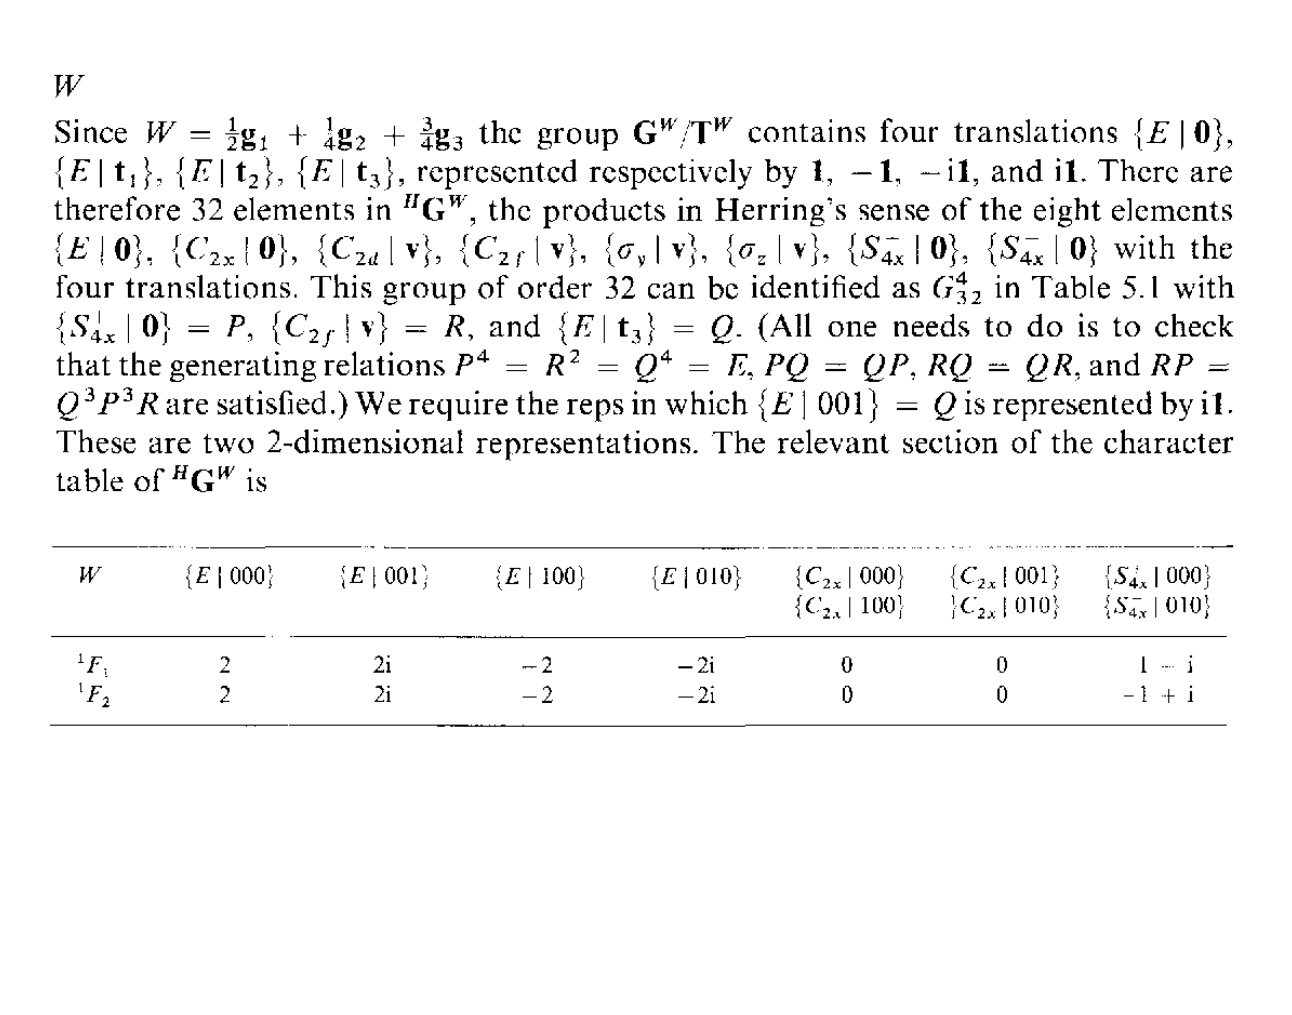
\includegraphics[width=0.92\textwidth]{c3_wchar_p1.png}
\end{figure}
\begin{figure}[H]
\centering
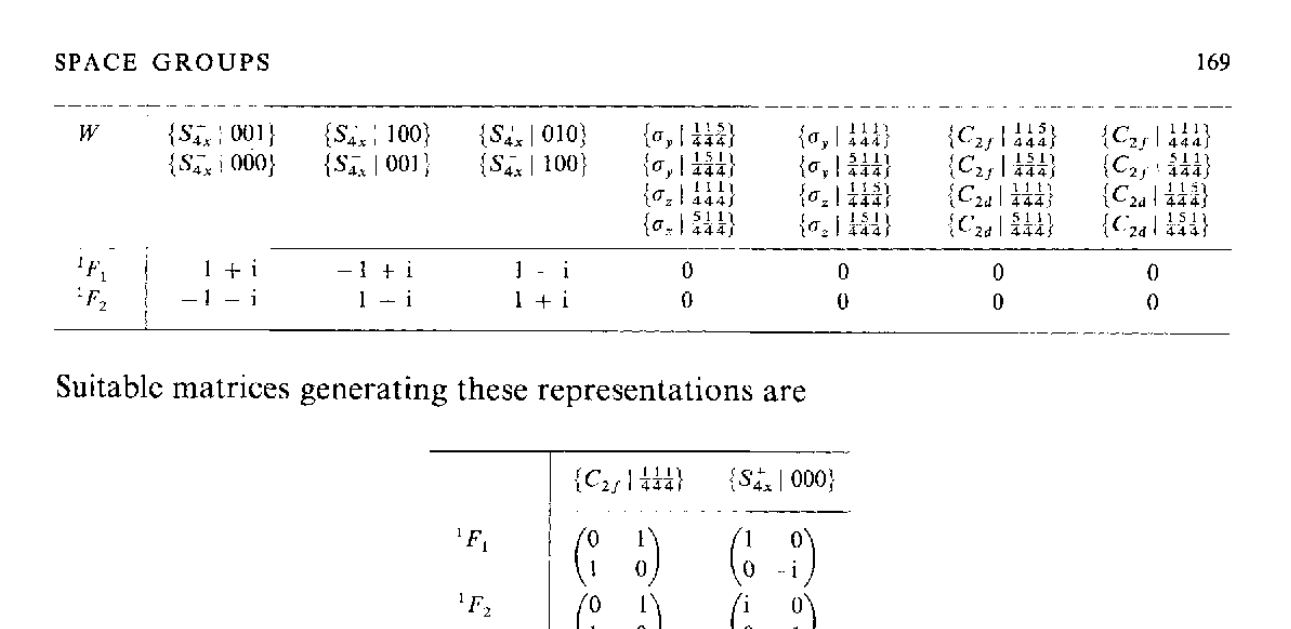
\includegraphics[width=0.92\textwidth]{c3_wchar_p2.png}
\caption*{\textbf{W 点}\ ${}^{H}\mathbf{G}^{W}$ 的特征标表（原书扫描占位，跨第 168--169 页）。}
\end{figure}

生成这些表示的合适矩阵是
\begin{center}
\begin{tabular}{lcc}
 & $\{C_{2f} \mid {\frac{1}{4}}{\frac{1}{4}}{\frac{1}{4}}\}$ & $\{S^{+}_{4x} \mid 000\}$\\[0.5ex]
${}^{1}\Gamma_{1}$ & $\begin{pmatrix} 0 & 1\\ 1 & 0 \end{pmatrix}$ & $\begin{pmatrix} 1 & 0\\ 0 & -i \end{pmatrix}$\\[2ex]
${}^{1}\Gamma_{2}$ & $\begin{pmatrix} 0 & 1\\ 1 & 0 \end{pmatrix}$ & $\begin{pmatrix} i & 0\\ 0 & -1 \end{pmatrix}$
\end{tabular}
\end{center}

\subsection*{X}

由于 $X = (\frac{1}{2}0\frac{1}{2})$，群 ${}^{H}\mathbf{G}^{X}$ 含有两个平移 $\{E \mid \mathbf{0}\}$ 与 $\{E \mid \mathbf{t}_{1}\}$，分别由 $\mathbf{1}$ 与 $-\mathbf{1}$ 表示。于是 ${}^{H}\mathbf{G}^{X}$ 中有 32 个元素，即 16 个元素 $\{E \mid \mathbf{0}\}$、$\{C_{2y} \mid \mathbf{0}\}$、$\{C^{+}_{4y} \mid \mathbf{v}\}$、$\{C_{2x} \mid \mathbf{0}\}$、$\{C_{2z} \mid \mathbf{0}\}$、$\{C_{2c} \mid \mathbf{v}\}$、$\{C_{2e} \mid \mathbf{v}\}$、$\{I \mid \mathbf{v}\}$、$\{\sigma_{y} \mid \mathbf{v}\}$、$\{S^{+}_{4y} \mid \mathbf{0}\}$、$\{\sigma_{x} \mid \mathbf{v}\}$、$\{\sigma_{z} \mid \mathbf{v}\}$、$\{\sigma_{dc} \mid \mathbf{0}\}$ 与 $\{\sigma_{de} \mid \mathbf{0}\}$ 与这两个平移在 Herring 意义下的乘积。这个 32 阶的群可以辨认为表 5.1 中的 $G^{2}_{32}$，取 $\{\sigma_{x} \mid \mathbf{v}\} = P$、$\{S^{+}_{4y} \mid \mathbf{0}\} = Q$、$\{C_{2x} \mid \mathbf{0}\} = R$。我们需要的是 $\{E \mid \mathbf{t}_{1}\} = P^{2}$ 由 $-\mathbf{1}$ 表示的那些表示。这是四个二维表示。${}^{H}\mathbf{G}^{X}$ 的特征标表的有关部分为

\begin{figure}[H]
\centering
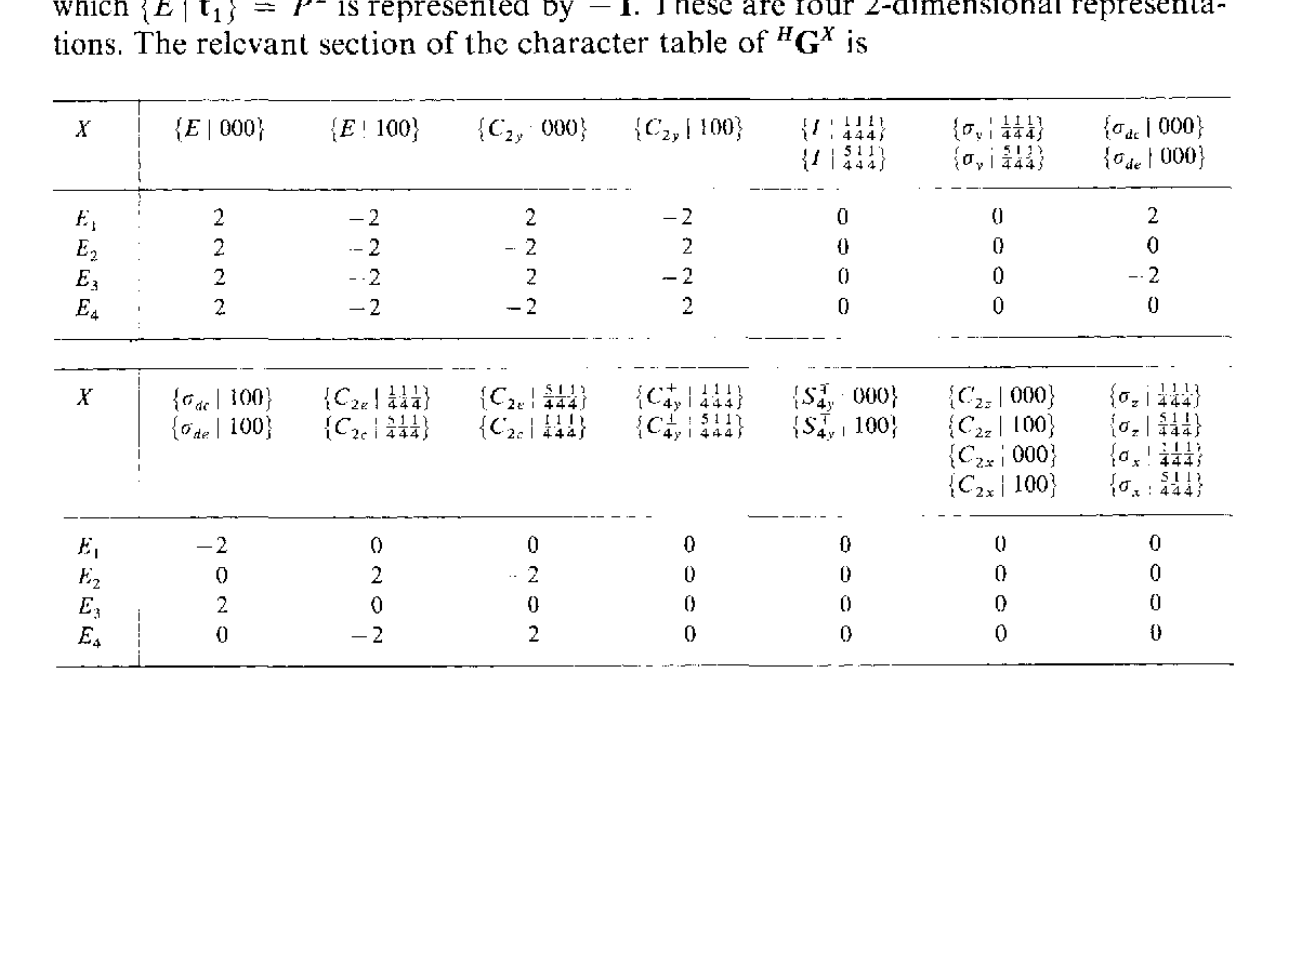
\includegraphics[width=0.92\textwidth]{c3_xchar.png}
\caption*{\textbf{X 点}\ ${}^{H}\mathbf{G}^{X}$ 的特征标表（原书扫描占位）。}
\end{figure}

生成这些表示的合适矩阵是
\begin{center}
\begin{tabular}{lccc}
 & $\{\sigma_{x} \mid {\frac{1}{4}}{\frac{1}{4}}{\frac{1}{4}}\}$ & $\{S^{+}_{4y} \mid 000\}$ & $\{C_{2x} \mid 000\}$\\[0.5ex]
$E_{1}$ & $\begin{pmatrix} 0 & -1\\ 1 & 0 \end{pmatrix}$ & $\begin{pmatrix} 0 & 1\\ 1 & 0 \end{pmatrix}$ & $\begin{pmatrix} 0 & 1\\ 1 & 0 \end{pmatrix}$\\[2ex]
$E_{2}$ & $\begin{pmatrix} 0 & -1\\ 1 & 0 \end{pmatrix}$ & $\begin{pmatrix} 0 & 1\\ -1 & 0 \end{pmatrix}$ & $\begin{pmatrix} 0 & 1\\ 1 & 0 \end{pmatrix}$\\[2ex]
$E_{3}$ & $\begin{pmatrix} 0 & -1\\ 1 & 0 \end{pmatrix}$ & $\begin{pmatrix} 0 & -1\\ -1 & 0 \end{pmatrix}$ & $\begin{pmatrix} 0 & 1\\ 1 & 0 \end{pmatrix}$\\[2ex]
$E_{4}$ & $\begin{pmatrix} 0 & -1\\ 1 & 0 \end{pmatrix}$ & $\begin{pmatrix} 0 & -1\\ 1 & 0 \end{pmatrix}$ & $\begin{pmatrix} 0 & 1\\ 1 & 0 \end{pmatrix}$
\end{tabular}
\end{center}

\subsection*{L}

由于 $L = (\frac{1}{2}\frac{1}{2}\frac{1}{2})$，群 ${}^{H}\mathbf{G}^{L}$ 含有两个平移 $\{E \mid \mathbf{0}\}$ 与 $\{E \mid \mathbf{t}_{1}\}$，分别由 $\mathbf{1}$ 与 $-\mathbf{1}$ 表示。该群阶为 24，同构于 $3m\ (C_{3v}) \otimes \mathbf{J} \otimes \mathbf{T}_{1}$，其中 $3m\ (C_{3v})$ 含有六个元素 $\{E \mid \mathbf{0}\}$、$\{C^{\pm}_{31} \mid \mathbf{0}\}$、$\{\sigma_{db} \mid \mathbf{0}\}$、$\{\sigma_{dc} \mid \mathbf{0}\}$、$\{\sigma_{df} \mid \mathbf{0}\}$，$\mathbf{J}$ 含有 $\{E \mid \mathbf{0}\}$ 与 $\{I \mid \mathbf{v}\}$，$\mathbf{T}_{1}$ 含有两个平移 $\{E \mid \mathbf{0}\}$ 与 $\{E \mid \mathbf{t}_{1}\}$。因此有六个小表示，${}^{H}\mathbf{G}^{L}$ 的特征标表的有关部分由表 2.2 可见为
\begin{center}
\begin{tabular}{lcccccc}
$L$ & $\{E \mid 000\}$ & $\{C^{\pm}_{31} \mid 000\}$ & $\begin{array}{c}\{\sigma_{db} \mid 000\}\\ \{\sigma_{dc} \mid 000\}\\ \{\sigma_{df} \mid 000\}\end{array}$ & $\{I \mid {\frac{1}{4}}{\frac{1}{4}}{\frac{1}{4}}\}$ & $\{S^{\mp}_{61} \mid {\frac{1}{4}}{\frac{1}{4}}{\frac{1}{4}}\}$ & $\begin{array}{c}\{C_{2b} \mid {\frac{1}{4}}{\frac{1}{4}}{\frac{1}{4}}\}\\ \{C_{2e} \mid {\frac{1}{4}}{\frac{1}{4}}{\frac{1}{4}}\}\\ \{C_{2f} \mid {\frac{1}{4}}{\frac{1}{4}}{\frac{1}{4}}\}\end{array}$\\
$A_{1g}$ & $1$ & $1$ & $1$ & $1$ & $1$ & $1$\\
$A_{2g}$ & $1$ & $1$ & $-1$ & $1$ & $1$ & $-1$\\
$E_{g}$ & $2$ & $-1$ & $0$ & $2$ & $-1$ & $0$\\
$A_{1u}$ & $1$ & $1$ & $1$ & $-1$ & $-1$ & $-1$\\
$A_{2u}$ & $1$ & $1$ & $-1$ & $-1$ & $-1$ & $1$\\
$E_{u}$ & $2$ & $-1$ & $0$ & $-2$ & $1$ & $0$
\end{tabular}
\end{center}
二维表示的生成矩阵可由表 2.3 得到。可以看到，碰巧 $Fd3m$ 中属于 $Q$ 和 $L$ 的表示的形式与 $Fm3m$ 中的完全一样。我们给出的关于这种情况何时必然发生的规则因此是充分的但不必要的；从这个例子我们看到，即使 $\mathbf{k}_{1}$ 位于布里渊区面上且空间群是非点式的，$\mathbf{G}^{\mathbf{k}_{1}}$ 的小表示偶尔也与 $\overline{\mathbf{G}}^{\mathbf{k}_{1}}$ 的表示具有相同的形式。


% 第四章
\chapter{用不变子群的表示表示群的表示}
% 第四章引言 + 4.1 诱导表示

在第三章的最后两节中，我们只对空间群的表示理论给出了并不完全的叙述。若干论证仅以梗概给出，还有一些论断未加证明。这样处理有几个原因。第一，我们觉得对某些读者来说第三章的叙述已经足够；的确，一个完全严格的论述的细节往往会把读者的注意力从中心议题上引开，使他在晦涩上的所失与在精确上的所得一样多。第二，完全严格的方案将适用于更广的群论背景，不仅对经典空间群有用，对其他应用也有用。因此，用一套不局限于空间群的普遍记号、并使之独立于上一章的那些特殊考虑来陈述完整的群论，似乎是明智的。

因此，本章的目的是以完全普遍的方式处理具有不变子群的群的表示理论；空间群是它的一个特例，其不变子群是三维平移群，因而是 Abel 群。这一补充理论将使我们能够填补上一章的空白，主要是证明为求空间群的表示而概述的方案确实产生全部表示——既不多也不少，也没有与其它表示等价的赝品——同时说明如何由已列成表的小表示得到精确矩阵形式的完全表示。附带地，这一理论还使我们能更容易地讨论固体理论中另外一些有趣的问题，例如表示的实性以及表示之间的内直积。实性之所以重要，是因为它有助于研究晶体中由于时间反演对称而引起的单个粒子或准粒子态的简并（Herring 1937\textit{a}, Wigner 1932）。内直积之所以重要，是因为它有助于确定固体中涉及电子、声子、磁振子等的各种过程的选择定则（Elliott and Loudon 1960）。

\section{诱导表示}

设 $\mathbf{G}$ 是一个群，$\mathbf{K}_{1}$ 是 $\mathbf{G}$ 的一个不一定是 invariant 的子群。例如 $\mathbf{G}$ 可以是一个空间群，而 $\mathbf{K}_{1}$ 是布里渊区中矢量 $\mathbf{k}_{1}$ 的小群。把 $\mathbf{K}_{1}$ 的元素记作 $k_{a}$，并把 $\mathbf{G}$ 写成
\begin{equation*}
\mathbf{G} = \sum_{\alpha}p_{\alpha}\mathbf{K}_{1},
\tag{4.1.1}
\end{equation*}
其中 $p_{\alpha}$ 是左陪集代表，我们假定对一切 $\alpha$ 一次性选定；例如总取 $p_{1} = e$（恒等元），并且每当我们写 $p_{\lambda}$ 时，指的都是式 (4.1.1) 展开中陪集 $p_{\lambda}\mathbf{K}_{1}$ 所对应的那一个陪集代表。

\noindent\textbf{定理 4.1.1}\quad 每个元素 $g \in \mathbf{G}$ 都可以表示成 $g = k_{b}p^{-1}_{\lambda}$，其中 $b$ 与 $\lambda$ 由 $g$ 唯一确定。

因为由刚才从式 (4.1.1) 推得的结果，$g^{-1} = p_{\lambda}k_{s}$，其中 $\lambda$ 与 $s$ 由 $g^{-1}$ 唯一确定。于是 $g = k^{-1}_{s}p^{-1}_{\lambda} = k_{b}p^{-1}_{\lambda}$，其中由于 $\mathbf{K}_{1}$ 是群，$k_{b} = k^{-1}_{s} \in \mathbf{K}_{1}$，定理得证。

现设 $\Omega_{1}$ 是在 $\mathbf{K}_{1}$ 下不可约的、维数为 $d_{j}$ 的矢量空间，取基 $\langle \phi_{r} |$（$r = 1$ 到 $d_{j}$），使得对一切 $k_{a} \in \mathbf{K}_{1}$
\begin{equation*}
k_{a}\phi_{r} = \sum^{d_{j}}_{p=1}\phi_{p}\Gamma^{j}(k_{a})_{pr}.
\tag{4.1.2}
\end{equation*}
把 $k_{a}$ 在表示 $\Gamma^{j}$ 中的特征标记作 $\chi^{j}(k_{a})$。再设 $\Omega$ 表示由 $d_{j}|\mathbf{G}|/|\mathbf{K}_{1}|$ 个函数 $\phi_{\alpha r}$ 张成的矢量空间，其中对一切 $\alpha$ 与 $r$
\begin{equation*}
\phi_{\alpha r} = p_{\alpha}\phi_{r}.
\tag{4.1.3}
\end{equation*}
式 (4.1.3) 是函数恒等式，即对相同的自变量，$\phi_{\alpha r}$ 与 $p_{\alpha}\phi_{r}$ 取相同的值。在第三章 3.7 节定义形如 $\{T_{i} \mid \mathbf{x}_{i}\}\psi_{\mathbf{k}}$ 的函数时，我们用的正是同样的手法。

\noindent\textbf{定理 4.1.2}\quad $\Omega$ 在 $\mathbf{G}$ 下不变。

因为写 $g = p_{\lambda}k_{s}$，则 $g\phi_{\tau r} = p_{\lambda}k_{s}p_{\tau}\phi_{r} = p_{\gamma}k_{t}\phi_{r}$，其中 $\gamma$ 与 $t$ 由 $g$ 与 $\tau$ 唯一确定。于是用式 (4.1.2) 与 (4.1.3) 得
\begin{equation*}
\begin{aligned}
g\phi_{\tau r} &= p_{\gamma}\sum_{p}\phi_{p}\Gamma^{j}(k_{t})_{pr}\\
&= \sum_{p}\phi_{\gamma p}\Gamma^{j}(k_{t})_{pr}.
\end{aligned}
\tag{4.1.4}
\end{equation*}
式 (4.1.4) 定义了所谓 $\Gamma^{j}$ 在 $\mathbf{G}$ 中的\textit{诱导表示}（induced representation），方便起见记作 $\Gamma^{j} \uparrow \mathbf{G}$，其特征标记作 $\chi(g)$。它的维数是 $d_{j}|\mathbf{G}|/|\mathbf{K}_{1}|$。式 (4.1.4) 的含义是：若 $g$ 把基函数 $\phi_{\tau r}$ 变到 $\Omega$ 的另一个基函数上，则表示矩阵的相应元素由 $\mathbf{K}_{1}$ 的表示矩阵给出。

现在应当清楚，空间群的表示事实上就是小群的小表示的诱导表示。这样我们已经完成了任务的一部分：说明如何由列成表的小群小表示得到空间群表示的详细矩阵形式。所涉步骤由式 (4.1.1)--(4.1.4) 概括，而表示的不可约性由下一节给出的判据处理。

\noindent\textbf{定理 4.1.3}\quad 定义 $\Omega_{\alpha}$ 为由 $d_{j}$ 个函数 $\phi_{\alpha r}$（$r = 1$ 到 $d_{j}$）张成的矢量空间。则对任意固定的 $\alpha$，$\Omega_{\alpha}$ 在子群 $\mathbf{K}_{\alpha} = \{p_{\alpha}k_{a}p^{-1}_{\alpha};\ k_{a} \in \mathbf{K}_{1}\}$ 下不可约。

因为利用式 (4.1.2) 与 (4.1.3)，
\begin{equation*}
p_{\alpha}k_{a}p^{-1}_{\alpha}\phi_{\alpha r} = p_{\alpha}k_{a}\phi_{r} = \sum_{s}\phi_{\alpha s}\Gamma^{j}(k_{a})_{sr}.
\tag{4.1.5}
\end{equation*}
式 (4.1.5) 的含义是：$p_{\alpha}k_{a}p^{-1}_{\alpha}$ 在基 $\langle \phi_{\alpha r} |$ 下的代表矩阵是 $\Gamma^{j}(k_{a})$。而矩阵群 $\Gamma^{j}(k_{a})$ 是不可约的（按定义），定理得证。

子群 $\mathbf{K}_{\alpha}$ 可以写成 $p_{\alpha}\mathbf{K}_{1}p^{-1}_{\alpha}$ 的形式。因此每个子群 $\mathbf{K}_{\alpha}$（$\alpha = 1$ 到 $|\mathbf{G}|/|\mathbf{K}_{1}|$）都具有下列性质：

(i) 它与 $\mathbf{K}_{1}$ 同阶。

(ii) 它在 $\mathbf{G}$ 下与 $\mathbf{K}_{1}$ 共轭，从而与集合 $\mathbf{K}_{\alpha}$ 中其他每个成员共轭（因为共轭是等价关系）。

(iii) 只要各子群互不相同，每一个都与分解 (4.1.1) 中的一个且只有一个陪集 $p_{\alpha}\mathbf{K}_{1}$ 一一对应。

我们认出以前遇到过这种情形。因为若把 $\mathbf{G}$ 认同于空间群的同形点群 $\mathbf{F}$，把 $\mathbf{K}_{1}$ 认同于 $\mathbf{k}_{1}$ 的小陪群，则 $\mathbf{K}_{\alpha}$ 可以认同为 $\mathbf{k}_{\alpha}$ 的小陪群，其中 $\mathbf{k}_{\alpha}$ 是 $\mathbf{k}_{1}$ 的星中与陪集 $p_{\alpha}\mathbf{K}_{1}$ 相应的成员。

\noindent\textbf{定理 4.1.4}\quad （Johnston 不可约性判据）\ 把 $g$ 在 $\Omega_{\alpha}$ 中的特征标记作 $\chi_{\alpha}(g)$，于是 $g$ 在 $\Gamma^{j} \uparrow \mathbf{G}$ 中的特征标 $\chi(g) = \sum_{\alpha}\chi_{\alpha}(g)$。那么只要对一切满足 $\alpha \neq \beta$ 的对 $(\alpha, \beta)$ 有
\begin{equation*}
\sum_{t}\chi^{*}_{\alpha}(t)\chi_{\beta}(t) = 0
\tag{4.1.6}
\end{equation*}
（对每一组选定的 $\alpha, \beta$，对 $t$ 的求和取遍 $\mathbf{K}_{\alpha} \cap \mathbf{K}_{\beta}$ 的所有元素），$\Omega$ 就在 $\mathbf{G}$ 下不可约。

Johnston (1960) 给出的这个有用定理的证明如下。

由定理 1.3.8，$\Omega$ 在 $\mathbf{G}$ 下不可约当且仅当
\begin{equation*}
\sum_{g}\chi^{*}(g)\chi(g) = |\mathbf{G}|,
\tag{4.1.7}
\end{equation*}
其中对 $g$ 的求和取遍 $\mathbf{G}$ 的所有元素。也就是说，若
\begin{equation*}
\sum_{\alpha}\sum_{g}|\chi_{\alpha}(g)|^{2} + \sum_{\alpha \neq \beta}\sum_{g}\left\{\chi^{*}_{\alpha}(g)\chi_{\beta}(g)\right\} = |\mathbf{G}|.
\tag{4.1.8}
\end{equation*}
由式 (4.1.4) 显然，若 $g$ 可写成 $p_{\tau}k_{t}p^{-1}_{\tau}$，则
\begin{equation*}
\chi_{\tau}(g) = \chi^{j}(k_{t}),
\tag{4.1.9a}
\end{equation*}
否则
\begin{equation*}
\chi_{\tau}(g) = 0.
\tag{4.1.9b}
\end{equation*}
于是 $\chi_{\tau}(g) = \chi^{j}(k_{t})$ 若 $g \in \mathbf{K}_{\tau}$ 且 $g = p_{\tau}k_{t}p^{-1}_{\tau}$，而对一切不属于 $\mathbf{K}_{\tau}$ 的 $g$ 它为零。由此
\begin{equation*}
\sum_{\alpha}\sum_{g}|\chi_{\alpha}(g)|^{2} = \sum_{\alpha}\sum_{a}|\chi^{j}(k_{a})|^{2} = \sum_{\alpha}|\mathbf{K}_{1}| = |\mathbf{G}|.
\end{equation*}
（由于 $\Gamma^{j}$ 在 $\mathbf{K}_{1}$ 下不可约，定理 1.3.8 成立，并且在对 $a$ 求和时已用到它。）

因此 $\Gamma^{j} \uparrow \mathbf{G}$ 不可约当且仅当
\begin{equation*}
\sum_{\alpha \neq \beta}\sum_{g}\chi^{*}_{\alpha}(g)\chi_{\beta}(g) = 0.
\tag{4.1.10}
\end{equation*}
特别地，若对所有满足 $\alpha \neq \beta$ 的 $\alpha, \beta$ 都有
\begin{equation*}
\sum_{g}\chi^{*}_{\alpha}(g)\chi_{\beta}(g) = 0
\tag{4.1.11}
\end{equation*}
则 $\Gamma^{j} \uparrow \mathbf{G}$ 不可约。

借助式 (4.1.9)，式 (4.1.11) 左端可能出现非零项的唯一情形是 $g$ 同时属于 $\mathbf{K}_{\alpha}$ 与 $\mathbf{K}_{\beta}$。这就给出条件 (4.1.6)，定理得证。

\noindent\textbf{推论}

（i）若 $\mathbf{K}_{1}$ 在 $\mathbf{G}$ 中不变，则对一切 $\alpha$ 有 $\mathbf{K}_{\alpha} = \mathbf{K}_{1}$，条件 (4.1.6) 变为
\begin{equation*}
\sum_{a}\chi^{*}_{\alpha}(k_{a})\chi_{\beta}(k_{a}) = 0
\tag{4.1.12}
\end{equation*}
对一切满足 $\alpha \neq \beta$ 的 $\alpha, \beta$ 成立。若由基 $\langle \phi_{\alpha r} |$（$\alpha = 1$ 到 $|\mathbf{G}|/|\mathbf{K}_{1}|$）张成的 $\mathbf{K}_{1}$ 的不可约表示彼此不等价，则上式满足。

（ii）条件 (4.1.6) 对每一对满足 $\alpha \neq \beta$ 的 $\alpha, \beta$ 涉及对群 $\mathbf{K}_{\alpha} \cap \mathbf{K}_{\beta}$ 全部元素的求和，要求该和为零。我们即将证明：若对 $\mathbf{K}_{\alpha} \cap \mathbf{K}_{\beta}$ 的某个子群 $\mathbf{H}_{\alpha\beta}$ 有
\begin{equation*}
\sum_{h}\chi^{*}_{\alpha}(h)\chi_{\beta}(h) = 0,
\tag{4.1.13}
\end{equation*}
（对 $h$ 的求和取遍 $\mathbf{H}_{\alpha\beta}$ 的所有元素），则该和为零。若能选取 $\mathbf{H}_{\alpha\beta}$ 为对一切对 $\alpha, \beta$ 都相同的 $\mathbf{G}$ 的子群 $\mathbf{H}$，这一判据特别有用。

为了证明式 (4.1.13) 足以蕴含特定对 $\alpha, \beta$ 的式 (4.1.6)，更仔细地考察式 (4.1.13) 的含义：它说的是 $\mathbf{H}_{\alpha\beta}$ 的两个表示——一个以 $\langle \phi_{\alpha r} |$ 为基、另一个以 $\langle \phi_{\beta r} |$ 为基——当限制在 $\mathbf{H}_{\alpha\beta}$ 上时没有共同的分量。

\noindent\textbf{定理 4.1.5}\quad （Frobenius 互反定理）\ 设 $\Gamma$ 是 $\mathbf{G}$ 的表示，特征标为 $\chi^{\Gamma}(g)$；则 $\Gamma$ 在 $\Gamma^{j} \uparrow \mathbf{G}$ 分解为 $\mathbf{G}$ 的不可约表示时出现的次数，等于表示 $\Gamma^{j}$ 在 $\Gamma$ 限制到 $\mathbf{K}_{1}$（记作 $\Gamma \downarrow \mathbf{K}_{1}$）的分解中出现的次数。

定理证明如下。$\Gamma$ 在 $\Gamma^{j} \uparrow \mathbf{G}$ 中出现的次数等于交织数 $(1/|\mathbf{G}|)\sum_{g}\chi(g)\chi^{\Gamma}(g^{-1})$：
\begin{equation*}
= \frac{1}{|\mathbf{G}|}\sum_{g}\sum_{\alpha}\chi_{\alpha}(g)\chi^{\Gamma}(g^{-1})
\tag{4.1.14}
\end{equation*}
\begin{equation*}
= \frac{1}{|\mathbf{G}|}\sum_{a}\sum_{\alpha}\chi^{j}(k_{a})\chi^{\Gamma}(p_{\alpha}k^{-1}_{a}p^{-1}_{\alpha})
\tag{4.1.15}
\end{equation*}
\begin{equation*}
= \frac{1}{|\mathbf{K}_{1}|}\sum_{a}\chi^{j}(k_{a})\chi^{\Gamma}(k^{-1}_{a}),
\tag{4.1.16}
\end{equation*}
这是一个交织数，表示 $\Gamma^{j}$ 在 $\Gamma \downarrow \mathbf{K}_{1}$ 中出现的次数。从 (4.1.14) 到 (4.1.15) 我们用了式 (4.1.9)，从 (4.1.15) 到 (4.1.16) 用了 $k^{-1}_{a}$ 与 $p_{\alpha}k^{-1}_{a}p^{-1}_{\alpha}$ 属于 $\mathbf{K}_{1}$ 的同一类这一事实。

% 4.2 具有不变子群的群
\section{具有不变子群的群}

本节考虑具有真不变子群 $\mathbf{T}$ 的群 $\mathbf{G}$ 的若干性质。（若 $\mathbf{T}$ 是 Abel 群，则 $\mathbf{G}$ 具有与空间群相似的结构；例如见式 (3.5.2)。）

我们把 $\mathbf{G}$ 关于 $\mathbf{T}$ 的左陪集展开：
\begin{equation*}
\mathbf{G} = \sum_{x}r_{x}\mathbf{T},
\tag{4.2.1}
\end{equation*}
其中一如既往地假定左陪集代表 $r_{x}$ 一次性选定。我们总取 $r_{1} = e$（$\mathbf{G}$ 的恒等元），并把 $\mathbf{T}$ 的恒等元记作 $t_{1} = e$。

若能把左陪集代表选成一个群 $\mathbf{F}$，我们将假定已作了这样的选择。\footnote{常常有这样的情形：在左陪集代表 $r_{x}$ 的各种选法中，有些选法构成群，有些不构成。例如点群 $432\ (O)$ 可以展开为
\begin{center}
$E\mathbf{T} + C^{+}_{31}\mathbf{T} + C^{-}_{31}\mathbf{T} + C_{2b}\mathbf{T} + C_{2e}\mathbf{T} + C_{2f}\mathbf{T}$
\end{center}
其中 $\mathbf{T}$ 是点群 $222\ (D_{2})\ (= E + C_{2x} + C_{2y} + C_{2z})$；它也可以展开为
\begin{center}
$E\mathbf{T} + C^{+}_{31}\mathbf{T} + C^{-}_{31}\mathbf{T} + C_{2a}\mathbf{T} + C_{2c}\mathbf{T} + C_{2d}\mathbf{T}$。
\end{center}
在第一种情形，$r_{\alpha}$ 构成点群 $32\ (D_{3})$（诚然取向非标准）。（——中译者注：本注按原书脚注照录，第二式中 $C^{+}_{31}$ 的上标疑为 $C^{\pm}_{31}$ 之误排。）}

\noindent\textbf{定义 4.2.1}\quad 若群 $\mathbf{G}$ 关于不变子群 $\mathbf{T}$ 的左陪集代表 $r_{\alpha}$ 可以选成一个子群 $\mathbf{F}$，则称 $\mathbf{G}$ 是 $\mathbf{T}$ 与 $\mathbf{F}$ 的\textit{半直积}（semi-direct product），记作 $\mathbf{G} = \mathbf{T} \wedge \mathbf{F}$。

（半直积的等价定义见定义 1.2.17。）然而，无论 $\mathbf{G}$ 是不是半直积，本节的内容都成立。

把 $\mathbf{G}$ 的元素记作 $(r_{\alpha}t_{a})$（这些记号不要与 Seitz 空间群算符混淆）。其乘法规则为
\begin{equation*}
(r_{\alpha}t_{a})(r_{\beta}t_{b}) = (r_{\alpha\beta}\, t_{\alpha\beta}[t_{a}]_{\beta}t_{b}),
\tag{4.2.2}
\end{equation*}
其中由于 $\mathbf{T}$ 不变，$[t_{a}]_{\beta} = r^{-1}_{\beta}t_{a}r_{\beta} \in \mathbf{T}$，且
\begin{equation*}
r_{\alpha}r_{\beta} = r_{\alpha\beta}t_{\alpha\beta},
\tag{4.2.3}
\end{equation*}
式 (4.2.3) 右端是元素 $r_{\alpha}r_{\beta} \in \mathbf{G}$ 分解为选定的左陪集代表之一 $r_{\alpha\beta}$ 与元素 $t_{\alpha\beta} \in \mathbf{T}$ 之积的唯一分解。对半直积群，对一切 $\alpha, \beta$ 有 $t_{\alpha\beta} = t_{1}$。

$\mathbf{G}$ 的恒等元是 $(r_{1}t_{1})$，由式 (4.2.2) 与 (4.2.3) 得到下列关系：
\begin{equation*}
[t_{a}]_{1} = t_{a}, \quad [t_{1}]_{\alpha} = t_{1}, \quad r_{\alpha 1} = r_{1\alpha} = r_{\alpha}, \quad\text{以及}\quad t_{\alpha 1} = t_{1\alpha} = t_{1};
\tag{4.2.4}
\end{equation*}
\begin{equation*}
[t_{a}]_{\alpha}[t_{b}]_{\alpha} = [t_{a}t_{b}]_{\alpha}
\tag{4.2.5}
\end{equation*}
以及
\begin{equation*}
[t^{-1}_{a}]_{\alpha} = \left([t_{a}]_{\alpha}\right)^{-1}.
\tag{4.2.6}
\end{equation*}
于是由群 $\mathbf{G}$ 的结合性（利用式 (4.2.2) 与 (4.2.5)）推得，对一切 $\alpha, \beta, \gamma$
\begin{equation*}
r_{\alpha\beta, \gamma} = r_{\alpha, \beta\gamma}
\tag{4.2.7}
\end{equation*}
以及
\begin{equation*}
t_{\alpha\beta, \gamma}[t_{\alpha\beta}]_{\gamma}[[t_{a}]_{\beta}]_{\gamma} = t_{\alpha, \beta\gamma}[t_{a}]_{\beta\gamma}t_{\beta\gamma}.
\tag{4.2.8}
\end{equation*}
注意由上述各方程组可得
\begin{equation*}
r_{\alpha, \beta 1} = r_{\alpha\beta, 1} = r_{\alpha\beta} = r_{1, \alpha\beta} = r_{1\alpha, \beta} = r_{\alpha, 1\beta} = r_{\alpha 1, \beta}
\tag{4.2.9}
\end{equation*}
但是，尽管
\begin{equation*}
t_{\alpha, \beta 1} = t_{1\alpha, \beta} = t_{\alpha, 1\beta} = t_{\alpha 1, \beta} = t_{\alpha\beta}, \quad t_{\alpha\beta, 1} = t_{1, \alpha\beta} = t_{1}.
\tag{4.2.10}
\end{equation*}
在式 (4.2.8) 中令 $a = 1$，得到一个对一切 $\alpha, \beta, \gamma$ 都重要的关系：
\begin{equation*}
t_{\alpha\beta, \gamma}[t_{\alpha\beta}]_{\gamma} = t_{\alpha, \beta\gamma}t_{\beta\gamma}.
\tag{4.2.11}
\end{equation*}
以下几点值得注意。$(r_{1}t_{a})$ 的逆是 $(r_{1}t^{-1}_{a})$。给定 $r_{\alpha}$，存在唯一的陪集代表 $r_{\bar{\alpha}}$ 使 $r_{\alpha\bar{\alpha}} = r_{\bar{\alpha}\alpha} = r_{1}$；$(r_{\alpha}t_{1})$ 的逆是 $(r_{\bar{\alpha}}t_{\alpha\bar{\alpha}})$。并且
\begin{equation*}
t_{\bar{\alpha}\alpha} = [t_{\alpha\bar{\alpha}}]_{\alpha},
\tag{4.2.12}
\end{equation*}
以及
\begin{equation*}
\left[[t_{a}]_{\alpha}\right]_{\bar{\alpha}} = t^{-1}_{\alpha\bar{\alpha}}t_{a}t_{\alpha\bar{\alpha}}.
\tag{4.2.13}
\end{equation*}
最后，容易验证
\begin{equation*}
r_{\alpha}t_{a}r^{-1}_{\alpha} = t_{\alpha\bar{\alpha}}[t_{a}]_{\bar{\alpha}}t^{-1}_{\alpha\bar{\alpha}}.
\tag{4.2.14}
\end{equation*}
我们把式 (4.2.14) 的右端取作 $[t_{a}]_{\alpha}^{-1}$ 的定义；它没有别的定义，因为 $r^{-1}_{\alpha}$ 不一定是选定的陪集代表之一。

\noindent\textbf{定理 4.2.1}\quad $(r_{\alpha}t_{a})$ 的逆是 $\left(r_{\bar{\alpha}}[t^{-1}_{a}]_{\bar{\alpha}}t^{-1}_{\alpha\bar{\alpha}}\right)$。

因为
\begin{equation*}
(r_{\alpha}t_{a})(r_{\bar{\alpha}}[t^{-1}_{a}]_{\bar{\alpha}}t^{-1}_{\alpha\bar{\alpha}}) = \left(r_{\alpha\bar{\alpha}}\, t_{\alpha\bar{\alpha}}[t_{a}]_{\bar{\alpha}}[t^{-1}_{a}]_{\bar{\alpha}}t^{-1}_{\alpha\bar{\alpha}}\right),
\end{equation*}
由式 (4.2.5) 及 $r_{\alpha\bar{\alpha}} = r_{1}$ 的事实，它等于恒等元。留给读者一个练习：利用式 (4.2.12) 与 (4.2.13) 验证 $\left(r_{\bar{\alpha}}[t^{-1}_{a}]_{\bar{\alpha}}t^{-1}_{\alpha\bar{\alpha}}\right) = (r_{\alpha}t_{a})^{-1}$ 亦可从 $(r_{\alpha}t_{a})(r_{\bar{\alpha}}t^{-1}_{a}t_{\alpha\bar{\alpha}}) = (r_{1}t_{1})$ 得出。

\noindent\textbf{定理 4.2.2}\quad 陪集代表的下标构成一个 $|\mathbf{G}|/|\mathbf{T}|$ 阶的群，记作 $\mathbf{R}$。它当然同构于因子群 $\mathbf{G}/\mathbf{T}$。

$\mathbf{R}$ 中的乘法规则是：若 $r_{\alpha}r_{\beta} \in r_{\gamma}\mathbf{T}$，则 $\alpha\beta = \gamma$。封闭性由构造即得，结合性由式 (4.2.7) 得到，恒等元是 1（见式 (4.2.4)），$\alpha$ 的逆是 $\bar{\alpha}$。

现在把 4.1 节的结果具体化到子群不变的情形。为此把 4.1 节的 $\mathbf{K}_{1}$、$p_{\alpha}$ 与 $\Gamma^{j}$ 分别认同为本节的 $\mathbf{T}$、$r_{\alpha}$ 与 $\mathbf{D}^{i}$。

$\mathbf{D}^{i}$ 是 $\mathbf{T}$ 的维数为 $d_{i}$ 的表示，基为 $\langle \phi_{r} |$，使得（见式 (4.1.2)）
\begin{equation*}
t_{a}\phi_{r} = \sum_{p}\phi_{p}\mathbf{D}^{i}(t_{a})_{pr}.
\tag{4.2.15}
\end{equation*}
函数 $\phi_{\alpha p} = r_{\alpha}\phi_{p}$（$\alpha = 1$ 到 $|\mathbf{G}|/|\mathbf{T}|$，$p = 1$ 到 $d_{i}$）张成一个在 $\mathbf{G}$ 下不变的矢量空间 $\mathbf{Q}$（见定理 4.1.2）。子群 $\mathbf{T}_{\alpha} = \{r_{\alpha}t_{a}r^{-1}_{\alpha};\ t_{a} \in \mathbf{T}\}$ 在 $\Omega_{\alpha}$ 上由
\begin{equation*}
t_{a}\phi_{\alpha r} = t_{a}r_{\alpha}\phi_{r} = r_{\alpha}[t_{a}]_{\alpha}\phi_{r} = \sum_{p}\phi_{\alpha p}\mathbf{D}^{i}([t_{a}]_{\alpha})_{pr}
\tag{4.2.16}
\end{equation*}
表示。式 (4.2.16) 蕴含
\begin{equation*}
\mathbf{D}^{i}_{\alpha}(t_{a}) = \mathbf{D}^{i}([t_{a}]_{\alpha}).
\tag{4.2.17}
\end{equation*}
由于此式对一切 $t_{a} \in \mathbf{T}$ 成立，称 $\mathbf{D}^{i}_{\alpha}$ 在 $\mathbf{G}$ 下\textit{共轭}于 $\mathbf{D}^{i}$。对 $\alpha = 1$ 到 $|\mathbf{G}|/|\mathbf{T}|$ 的表示集合 $\{D^{i}_{\alpha}\}$ 构成一族共轭表示。两个共轭表示可能等价；不过这并不影响随后的论证。

从一族共轭表示中选出的一组彼此不等价的表示的极大集合称为一个\textit{星}（star）（有些作者称之为轨道（orbit））。很容易看出这与已对空间群给出的定义一致。若把 $t_{a}$ 认同为平移 $\{E \mid \mathbf{t}\}$、把 $r_{\alpha}$ 认同为操作 $\{R \mid \mathbf{v}\}$，则
\begin{equation*}
[t_{a}]_{\alpha} \rightarrow \{R \mid \mathbf{v}\}^{-1}\{E \mid \mathbf{t}\}\{R \mid \mathbf{v}\} = \{E \mid R^{-1}\mathbf{t}\}.
\tag{4.2.18}
\end{equation*}
若把 $\mathbf{D}^{i}$ 认同为 $\Delta^{\mathbf{k}}$，则由式 (4.2.17)、(4.2.18)、(3.4.3) 与 (3.6.2)
\begin{equation*}
\begin{aligned}
\mathbf{D}^{i}_{\alpha}(t_{a}) &= \mathbf{D}^{i}([t_{a}]_{\alpha}) \rightarrow \Delta^{\mathbf{k}}(\{E \mid R^{-1}\mathbf{t}\})\\
&= \exp(-\mathrm{i}\mathbf{k} \cdot R^{-1}\mathbf{t})\mathbf{1} = \exp(-\mathrm{i}R\mathbf{k} \cdot \mathbf{t})\mathbf{1}\\
&= \Delta^{R\mathbf{k}}(\{E \mid \mathbf{t}\}) = \mathbf{D}^{i}_{\alpha}(t_{a}).
\end{aligned}
\tag{4.2.19}
\end{equation*}
两种定义的等价性现在来自如下事实：若 $R\mathbf{k} = \mathbf{k}$ 则 $\Delta^{R\mathbf{k}} \equiv \Delta^{\mathbf{k}}$，因此从平移群 $\mathbf{T}$ 的一族共轭表示中选出一组彼此不等价的极大表示集，就是构成一颗星——不管我们把星看作由表示组成还是由 $\mathbf{k}$ 矢量组成。

使 $D^{i}_{\gamma} \equiv D^{i}$ 的那些下标 $\gamma \in \mathbf{R}$ 的集合构成一个群 $\overline{\mathbf{K}}^{i}$，称为 $D^{i}$ 在 $\mathbf{G}$ 中的小陪群。与空间群术语（见定义 3.7.3）的对应是直接的：那里 $\mathbf{k}$ 在 $\mathbf{G}$ 中的小陪群 $\overline{\mathbf{G}}^{\mathbf{k}}$ 满足
\begin{equation*}
\begin{aligned}
\mathbf{D}^{i}_{\alpha\bar{\gamma}\bar{\alpha}}(t_{a}) &= \mathbf{D}^{i}([t_{a}]_{\alpha\bar{\gamma}\bar{\alpha}}) = \mathbf{D}^{i}\left(\left[[t_{a}]_{\alpha\bar{\gamma}\bar{\alpha}}\right]_{\alpha}\right)\\
&= \mathbf{D}^{i}([t_{a}]_{\alpha\gamma}) = \mathbf{D}^{i}_{\gamma}([t_{a}]_{\alpha}) = \mathbf{D}^{i}_{\gamma\alpha}(t_{a}),
\end{aligned}
\tag{4.2.19a}
\end{equation*}
在空间群理论中相应的结果是 $\overline{\mathbf{G}}^{R\mathbf{k}} = \{RSR^{-1};\ S \in \overline{\mathbf{G}}^{\mathbf{k}}\}$。

若一族共轭表示的所有成员互不等价，则小陪群仅由 1 组成。这对应于 $\mathbf{k}$ 是布里渊区的一般点。由方程
\begin{equation*}
\mathbf{K}^{i} = \sum_{\gamma \in \overline{\mathbf{K}}^{i}}r_{\gamma}\mathbf{T}
\tag{4.2.20}
\end{equation*}
定义的群 $\mathbf{K}^{i}$（其中 $\gamma$ 取遍小陪群）称为 $D^{i}$（$i$）在 $\mathbf{G}$ 中的\textit{小群}。小陪群同构于因子群 $\mathbf{K}^{i}/\mathbf{T}$。

现在考察由空间 $\mathbf{Q}$ 确定的诱导表示 $\mathbf{D}^{i} \uparrow \mathbf{G}$。与式 (4.1.4) 相应的方程是
\begin{equation*}
(r_{\alpha}t_{a})\phi_{\tau r} = \sum_{p}\phi_{\sigma p}\mathbf{D}^{i}(t_{\alpha\tau}[t_{a}]_{\tau})_{pr}
\tag{4.2.21}
\end{equation*}
其中 $\sigma = \alpha\tau$。

与式 (4.1.9) 相应的方程是
\begin{equation*}
\chi(r_{\alpha}t_{a}) = \delta_{\alpha 1}\sum_{\tau}\chi^{i}_{\tau}(t_{a}).
\tag{4.2.22}
\end{equation*}
也就是说，在 $\mathbf{D}^{i} \uparrow \mathbf{G}$ 中只有 $\mathbf{T}$ 的元素才有非零特征标；而在 $\mathbf{T}$ 中，每个元素的特征标是它在与 $D^{i}$ 共轭的一组完全表示上取的特征标之和。

由于 $\mathbf{T}$ 不变，Johnston 不可约性判据（定理 4.1.4）的推论 (i) 适用，并断言：若与 $D^{i}$ 共轭的表示集合中没有两个等价，则 $\mathbf{D}^{i} \uparrow \mathbf{G}$ 不可约。于是对空间群 $\mathbf{G}$，若 $\mathbf{k}$ 是布里渊区的一般点，则 $\Delta^{\mathbf{k}} \uparrow \mathbf{G}$ 不可约。

由式 (4.2.22) 可见
\begin{equation*}
(\mathbf{D}^{i} \uparrow \mathbf{G}) \downarrow \mathbf{T} = \sum_{\tau}D^{i}_{\tau}.
\tag{4.2.23}
\end{equation*}
当 $\mathbf{D}^{i} \uparrow \mathbf{G}$ 不可约时，$D^{i}_{\tau}$（$\tau = 1$ 到 $|\mathbf{G}|/|\mathbf{T}|$）彼此不等价，式 (4.2.23) 右端等于含 $D^{i}$ 的那颗星（简称星 $i$）。并且由 Frobenius 互反定理 4.1.5 得：$D^{i}_{\tau} \uparrow \mathbf{G}$ 与 $\mathbf{D}^{i} \uparrow \mathbf{G}$ 等价，因为按该定理 $D^{i}_{\tau} \uparrow \mathbf{G}$ 中含 $\Gamma$（任意一个含于 $\mathbf{D}^{i} \uparrow \mathbf{G}$ 的不可约表示）的次数等于 $\Gamma$ 限制后含 $D^{i}_{\tau}$ 的次数，与 $i$ 无关。

一般情形，当 $\mathbf{D}^{i} \uparrow \mathbf{G}$ 可约时，小陪群由 1 以外的元素组成。由式 (4.2.20) 可见它由 $|\mathbf{K}^{i}|/|\mathbf{T}|$ 个元素组成；这意味着在和 $\sum_{\tau}D^{i}_{\tau}$ 中，星 $i$ 将出现 $|\mathbf{K}^{i}|/|\mathbf{T}|$ 次。

至此我们已证明：当小陪群只含一个元素时，表示 $\mathbf{D}^{i} \uparrow \mathbf{G}$ 不可约，而且它不仅可以由 $D^{i}$ 诱导，也可以由星 $i$ 的任一成员诱导。这样的不可约表示限制到 $\mathbf{T}$ 上时，星中的每个成员恰好出现一次。并非 $\mathbf{G}$ 的每个表示都能这样得到，因为平移群存在含等价表示的共轭表示集合。这后一种情形正是接下来要讨论的。

% 4.3 小群理论
\section{小群理论}

与 4.2 节一样，设 $\mathbf{G}$ 是带不变子群 $\mathbf{T}$ 的群。本节旨在严格地建立求 $\mathbf{G}$ 的所有表示的方案，即第三章 3.7 节为空间群概述过的同一方案。方案如下：

（i）把 $\mathbf{T}$ 的表示分派成星 $i$。

（ii）从星 $i$ 中任意选一个表示 $D^{i}$。

（iii）确定 $i$ 在 $\mathbf{G}$ 中的小群 $\mathbf{K}^{i}$；记住 $\mathbf{K}^{i} = \sum_{\gamma}r_{\gamma}\mathbf{T}$，其中对 $\gamma$ 的求和取遍由满足 $D^{i}_{\gamma} \equiv D^{i}$ 的元素组成的小陪群 $\overline{\mathbf{K}}^{i}$。

（iv）（原书此处无 (iv)，编号如此。——中译者注）

（v）求 $\mathbf{K}^{i}$ 的表示，并把那些限制到 $\mathbf{T}$ 上给出 $D^{i}$ 的倍数者记为 $\Gamma^{i}_{j}$。它们称为 $\mathbf{K}^{i}$ 的\textit{小表示}（small representations）。

（vi）对每个 $j$ 确定 $\Gamma^{i}_{j} \uparrow \mathbf{G}$。做法是按 4.1 节确立的方法，把这里的 $\mathbf{K}^{i}$ 认同为该节的 $\mathbf{K}_{1}$，把这里的 $\Gamma^{i}_{j}$ 认同为该节的表示 $\Gamma^{j}$。

（vii）对每颗星 $i$ 重复 (ii) 到 (vi)。

上述方案的步骤 (i) 到 (iv) 已详细讨论过。为论证步骤 (v) 的合理性，先证明下面的引理。

\noindent\textbf{引理 4.3.1}\quad 若 $\Gamma^{i}_{j}$ 是 $\mathbf{K}^{i}$ 的表示，且 $\Gamma^{i}_{j} \downarrow \mathbf{T}$ 含有 $D^{i}$，则它只含 $D^{i}$（也许不止一次）。

首先注意，由 Frobenius 互反定理 4.1.5，$\Gamma^{i}_{j} \downarrow \mathbf{T}$ 含 $D^{i}$ 当且仅当 $\mathbf{D}^{i} \uparrow \mathbf{K}^{i}$ 含 $\Gamma^{i}_{j}$。

设 $\mathbf{D}^{i} \uparrow \mathbf{K}^{i} = \sum_{j}\lambda^{i}_{j}\Gamma^{i}_{j} = \Gamma$。定理于是断言：$\Gamma^{i}_{j} \downarrow \mathbf{T}$ 含 $D^{i}$ 恰 $\lambda^{i}_{j}$ 次。但由 $\Gamma$ 的定义，$\Gamma \downarrow \mathbf{T} = (\mathbf{D}^{i} \uparrow \mathbf{K}^{i}) \downarrow \mathbf{T}$ 是 $D^{i}$ 的倍数，因此每个含 $D^{i}$ 的 $\Gamma^{i}_{j} \downarrow \mathbf{T}$ 只能含 $D^{i}$，引理得证。

顺带地，我们还进一步证明了 $(|\mathbf{K}^{i}|/|\mathbf{T}|)D^{i} = \Gamma \downarrow \mathbf{T} = (\sum_{j}\lambda^{i}_{j}\Gamma^{i}_{j}) \downarrow \mathbf{T} = \sum_{j}(\lambda^{i}_{j})^{2}D^{i}$，从而 $\sum_{j}(\lambda^{i}_{j})^{2} = |\mathbf{K}^{i}|/|\mathbf{T}|$。

\noindent\textbf{定理 4.3.1}\quad 表示 $\Gamma^{i}_{j} \uparrow \mathbf{G}$（所有 $i$，所有 $j$）全都不可约；并且这样便得到 $\mathbf{G}$ 的所有表示，且一次也不多、一次也不少。

当然注意，对那些 $\overline{\mathbf{K}}^{i}$ 仅由恒等元组成的星 $i$，有 $\mathbf{K}^{i} = \mathbf{T}$；唯一的 $\Gamma^{i}_{j} = D^{i}$，且 $\mathbf{D}^{i} \uparrow \mathbf{G}$ 不可约，因此定理 4.3.1 把 4.2 节的最终结果作为平凡情形包含在内。

我们先证明 $\Gamma^{i}_{j} \uparrow \mathbf{G}$ 不可约。记住 $\mathbf{G} = \sum_{\alpha}p_{\alpha}\mathbf{K}^{i}$，其中 $p_{\alpha}$ 的特征性质是集合 $\{D^{i}_{\alpha}\}$ 构成 $D^{i}$ 的星。

$\Gamma^{i}_{j} \uparrow \mathbf{G}$ 的不可约性立刻由定理 4.1.4 的推论 (ii) 得到。取 $\mathbf{H}_{\alpha\beta} = \mathbf{T}$ 为 $\mathbf{K}^{i}_{\alpha} \cap \mathbf{K}^{i}_{\beta}$ 对一切 $\alpha \neq \beta$ 的公共子群，该推论断言：若
\begin{equation*}
\sum_{t_{a} \in \mathbf{T}}\chi^{i*}_{\alpha}(t_{a})\chi^{i}_{\beta}(t_{a}) = 0, \quad\text{对一切 } \alpha \neq \beta
\tag{4.3.1}
\end{equation*}
则 $\Gamma^{i}_{j} \uparrow \mathbf{G}$ 不可约。这里 $\chi^{i}_{\alpha}(t_{a})$ 是 $t_{a}$ 在由空间 $\Omega_{\alpha}$ 张成的表示（即可约表示 $\lambda^{i}_{j}D^{i}_{\alpha}$）中的特征标；类似地 $\chi^{i}_{\beta}(t_{a})$ 是 $t_{a}$ 在 $\lambda^{i}_{j}D^{i}_{\beta}$ 中的特征标。由引理 4.3.1，$\Gamma^{i}_{j}$ 限制到 $\mathbf{T}$ 上只含 $D^{i}$，因此 $\lambda^{i}_{j}D^{i}_{\alpha} = \lambda^{i}_{j}D^{i}_{\beta}$（对一切 $\alpha, \beta$），从而式 (4.3.1) 的左端是 $\left(\lambda^{i}_{j}\right)^{2}\sum_{t_{a}}\chi^{*}(t_{a})\chi(t_{a})$，其中 $\chi$ 是 $D^{i}$ 的特征标。由于 $D^{i}$ 不可约，此和等于 $|\mathbf{T}| > 0$；但 $\left(\lambda^{i}_{j}\right)^{2} \geq 1$，矛盾——因此该和为零，$\Gamma^{i}_{j} \uparrow \mathbf{G}$ 不可约。

尚需证明：对每颗星 $i$ 和所有小表示 $j$ 重复诱导过程，我们恰好一次地得到 $\mathbf{G}$ 的所有表示。需要考虑两点：第一，这样做是否会漏掉 $\mathbf{G}$ 的某个表示；第二，是否会重复计入某些表示。为排除第二种可能，先证两个引理。

\noindent\textbf{引理 4.3.2}\quad （限制的传递性）
\begin{equation*}
\left(\Delta^{i}_{j} \downarrow \mathbf{K}^{i}\right) \downarrow \mathbf{T} = \Delta^{i}_{j} \downarrow \mathbf{T}.
\tag{4.3.2}
\end{equation*}
这是因为两端由同一组矩阵组成。

\noindent\textbf{引理 4.3.3}\quad （诱导的传递性）
\begin{equation*}
(\mathbf{D}^{i} \uparrow \mathbf{K}^{i}) \uparrow \mathbf{G} \equiv \mathbf{D}^{i} \uparrow \mathbf{G}
\tag{4.3.3}
\end{equation*}
其中，由于 $\mathbf{D}^{i} \uparrow \mathbf{K}^{i} = \sum_{j}\lambda^{i}_{j}\Gamma^{i}_{j}$，式 (4.3.3) 的左端取为 $\sum_{j}\lambda^{i}_{j}(\Gamma^{i}_{j} \uparrow \mathbf{G}) = \sum_{j}\lambda^{i}_{j}\Delta^{i}_{j}$。

由式 (4.2.15) 之后的正文回顾：张成表示 $\mathbf{D}^{i} \uparrow \mathbf{G}$ 的基由函数 $r_{\alpha}\phi_{p} = \phi_{\alpha p}$（$\alpha = 1$ 到 $|\mathbf{G}|/|\mathbf{T}|$，$p = 1$ 到 $d_{i}$）组成，其中 $\langle \phi_{p} |$ 是 $D^{i}$ 的基。把这些函数按 $\alpha$ 分组，即知 $\mathbf{D}^{i} \uparrow \mathbf{G}$ 限制到 $\mathbf{T}$ 上由 $|\mathbf{G}|/|\mathbf{T}|$ 个块组成，每块都是 $D^{i}$。于是 $\mathbf{D}^{i} \uparrow \mathbf{G}$ 分解成不可约表示的形式必为
\begin{equation*}
\mathbf{D}^{i} \uparrow \mathbf{G} \equiv \sum_{j}\lambda^{i}_{j}\Delta^{i}_{j}.
\tag{4.3.4}
\end{equation*}
但 $\Delta^{i}_{j}$ 在 $\mathbf{G}$ 中不可约。因此由 Frobenius 互反定理，$\Delta^{i}_{j} \downarrow \mathbf{T}$ 恰含 $D^{i}$ $\lambda^{i}_{j}$ 次。

\noindent\textbf{引理 4.3.4}
\begin{equation*}
\Delta^{i}_{j} \downarrow \mathbf{T} = \sum_{\alpha}\lambda^{i}_{j}D^{i}_{\alpha}
\tag{4.3.5}
\end{equation*}
其中集合 $\{D^{i}_{\alpha}\}$ 构成 $D^{i}$ 的星。

上面已证明 $\Delta^{i}_{j} \downarrow \mathbf{T}$ 恰含 $D^{i}$ $\lambda^{i}_{j}$ 次；由于 $\Delta^{i}_{j}$ 是从 $\mathbf{K}^{i}$ 到 $\mathbf{G}$ 的诱导表示，故它必然以相同次数含有 $D^{i}$ 的星的全部成员。

现在很容易证明 $\Gamma^{i}_{j} \uparrow \mathbf{G} = \Delta^{i}_{j}$（所有 $i$，所有 $j$）彼此不等价。首先，设给定 $\Delta^{i_{1}}_{j_{1}}$ 与 $\Delta^{i_{2}}_{j_{2}}$，$i_{1} \neq i_{2}$，则由引理 4.3.4 及不同星的表示互不等价的事实，二者不可能等价。其次，设 $i_{1} = i_{2} = i$ 而 $j_{1} \neq j_{2}$：若 $\Delta^{i}_{j_{1}} \equiv \Delta^{i}_{j_{2}}$，则限制到 $\mathbf{T}$ 后仍等价，从而 $\lambda^{i}_{j_{1}} = \lambda^{i}_{j_{2}} = \lambda$，于是 $\Gamma^{i}_{j_{1}}$ 与 $\Gamma^{i}_{j_{2}}$ 限制后都含 $D^{i}$ 恰 $\lambda$ 次；由 $\sum_{j}(\lambda^{i}_{j})^{2} = |\mathbf{K}^{i}|/|\mathbf{T}|$ 及小表示的完全性可以排除这种情形（详细论证见原文），因此 $\Gamma^{i}_{j_{1}} \neq \Gamma^{i}_{j_{2}}$，等价性不成立。

最后还需证明没有遗漏。设 $\Delta$ 是 $\mathbf{G}$ 的任一不可约表示。由 Frobenius 互反定理，$(\Delta \downarrow \mathbf{T}) \uparrow \mathbf{G}$ 含 $\Delta$；而 $\Delta \downarrow \mathbf{T}$ 必含 $\mathbf{T}$ 的某个不可约表示 $D^{i}$，设其所在星为 $i$、次数为 $\mu$。由引理 4.3.3（传递性）与上面的构造，$\mathbf{D}^{i} \uparrow \mathbf{G}$（它等价于 $(\mathbf{D}^{i} \uparrow \mathbf{K}^{i}) \uparrow \mathbf{G} = \sum_{j}\lambda^{i}_{j}(\Gamma^{i}_{j} \uparrow \mathbf{G})$）在限制到 $\mathbf{T}$ 时含 $D^{i}$ 共 $|\mathbf{G}|/|\mathbf{T}|$ 次；按维数比较可知 $\Delta$ 必与某个 $\Gamma^{i}_{j} \uparrow \mathbf{G}$ 等价。因此没有遗漏。

\begin{equation*}
\sum_{i}\sum_{j}\left(\dim \Delta^{i}_{j}\right)^{2} = \sum_{i}\sum_{j}\left(|\mathbf{G}|/|\mathbf{K}^{i}|\right)^{2}\left(\lambda^{i}_{j}\right)^{2}d^{2}_{i} = \sum_{i}\frac{|\mathbf{G}|^{2}}{|\mathbf{K}^{i}||\mathbf{T}|}d^{2}_{i}
\end{equation*}
\begin{equation*}
= \frac{|\mathbf{G}|}{|\mathbf{T}|}\sum_{i}q_{i}d^{2}_{i} = \frac{|\mathbf{G}|}{|\mathbf{T}|}|\mathbf{T}| = |\mathbf{G}|.
\end{equation*}
定理 4.3.1 证毕。

% 4.4 小群的小表示
\section{小群的小表示}

我们已经确定，按上一节的记号，$\mathbf{G}$ 的每个表示都要通过对 $\mathbf{K}^{i}$ 的某个表示 $\Gamma^{i}_{j}$ 施行诱导来得到。的确，$\mathbf{G}$ 的每个表示由两个标记刻画：$i$（星的标记）与 $j$（小表示的标记）。3.4 节描述的方法构成一个方案；现在来说明如何具体求出小表示 $\Gamma^{i}_{j}$。

由于 $\Gamma^{i}_{j} \downarrow \mathbf{T} = \lambda^{i}_{j}D^{i}$，表示 $\Gamma^{i}_{j}$ 限制到 $\mathbf{T}$ 上是 $\lambda^{i}_{j}$ 个 $D^{i}$ 的直和。因此选取合适的基后可以写
\begin{equation*}
\Gamma^{i}_{j}(t_{a}) = \begin{pmatrix} \mathbf{D}^{i}(t_{a}) & 0 & \dots\\ 0 & \mathbf{D}^{i}(t_{a}) & \dots\\ \vdots & \vdots \end{pmatrix},
\tag{4.4.1}
\end{equation*}
即 $\lambda^{i}_{j}$ 个矩阵 $\mathbf{D}^{i}(t_{a})$ 的直和。于是只需求出 $\gamma \in \overline{\mathbf{K}}^{i}$ 的矩阵代表 $\Gamma^{i}_{j}(r_{\gamma})$；因为此后 $\mathbf{K}^{i}$ 的所有元素的矩阵代表都可以由乘法规则构造出来。分两种情形讨论。

\subsection*{情形 (i)．$\mathbf{T}$ 为 Abel 群}

这涵盖空间群的情形，事实上也涵盖一切具有真不变子群、且该子群是循环群直积的有限群。此时 $D^{i}$ 是一维的，$\Gamma^{i}_{j}$ 的维数等于 $\lambda^{i}_{j}$。而且 $\Gamma^{i}_{j}(t_{a})$ 等于 $\lambda^{i}_{j}D^{i}(t_{a})\mathbf{1}$。

现在回忆对一切 $\beta, \gamma, \delta \in \overline{\mathbf{K}}^{i}$ 必须成立的下列关系：
\begin{equation*}
r_{\gamma}r_{\delta} = r_{\gamma\delta}t_{\gamma\delta},
\tag{4.4.2}
\end{equation*}
\begin{equation*}
t_{\beta\gamma, \delta}[t_{\beta\gamma}]_{\delta} = t_{\beta, \gamma\delta}t_{\gamma\delta}
\tag{4.4.3}
\end{equation*}
（见式 (4.2.3) 与 (4.2.11)）。于是在表示 $\Gamma^{i}_{j}$ 中必须有
\begin{equation*}
\Gamma^{i}_{j}(r_{\gamma})\Gamma^{i}_{j}(r_{\delta}) = \Gamma^{i}_{j}(r_{\gamma\delta})\Gamma^{i}_{j}(t_{\gamma\delta})
\tag{4.4.4}
\end{equation*}
\begin{equation*}
= \mathbf{D}^{i}(t_{\gamma\delta})\Gamma^{i}_{j}(r_{\gamma\delta})
\tag{4.4.5}
\end{equation*}
以及
\begin{equation*}
\mathbf{D}^{i}(t_{\beta\gamma, \delta})\mathbf{D}^{i}([t_{\beta\gamma}]_{\delta}) = \mathbf{D}^{i}(t_{\beta, \gamma\delta})\mathbf{D}^{i}(t_{\gamma\delta}).
\tag{4.4.6}
\end{equation*}
但 $D^{i} \simeq D^{i}_{\delta}$，因为 $D^{i}$ 是一维的且 $\delta \in \overline{\mathbf{K}}^{i}$（等价的一维矩阵相等）。于是式 (4.4.6) 成为
\begin{equation*}
\mathbf{D}^{i}(t_{\beta\gamma, \delta})\mathbf{D}^{i}(t_{\beta\gamma}) = \mathbf{D}^{i}(t_{\beta, \gamma\delta})\mathbf{D}^{i}(t_{\gamma\delta}).
\tag{4.4.7}
\end{equation*}
现在考虑群 $\overline{\mathbf{K}}^{i}$。令 $\Gamma^{i}_{j}(r_{\gamma}) = \Lambda^{i}_{j}(\gamma)$、$\mathbf{D}^{i}(t_{\beta\gamma}) = \mu^{i}(\beta, \gamma)$，则式 (4.4.5) 与 (4.4.7) 成为
\begin{equation*}
\Lambda^{i}_{j}(\gamma)\Lambda^{i}_{j}(\delta) = \mu^{i}(\gamma, \delta)\Lambda^{i}_{j}(\gamma\delta)
\tag{4.4.8}
\end{equation*}
与
\begin{equation*}
\mu^{i}(\beta\gamma, \delta)\mu^{i}(\beta, \gamma) = \mu^{i}(\beta, \gamma\delta)\mu^{i}(\gamma, \delta).
\tag{4.4.9}
\end{equation*}
式 (4.4.8) 与 (4.4.9) 表明，复数 $\mu^{i}$ 构成 $\overline{\mathbf{K}}^{i}$ 的一个射影表示的因子系统。而且该射影表示的维数为 $\lambda^{i}_{j}$ 且不可约，因为 $\Gamma^{i}_{j}(r_{\gamma}) = \Lambda^{i}_{j}(\gamma)$ 已不可约。

顺带地，我们验证了：由于 $\sum_{j}\left(\lambda^{i}_{j}\right)^{2} = |\overline{\mathbf{K}}^{i}|$，$\overline{\mathbf{K}}^{i}$ 的这些射影表示的维数平方和等于 $\overline{\mathbf{K}}^{i}$ 的阶。

当元素 $r_{\gamma}$ 可以选成构成一个群时会出现简化。此时对一切 $\gamma, \delta \in \overline{\mathbf{K}}^{i}$ 有 $t_{\gamma\delta} = t_{1} = e$。因子系统由全为 1 的数组成，射影表示成为普通矢量表示。对空间群而言这总会发生在 $\mathbf{k}$ 为布里渊区内点或空间群为点式的情形。

\subsection*{情形 (ii)．$\mathbf{T}$ 为非 Abel 群}

若 $D^{i}$ 是一维表示，则理论恰如情形 (i)。的确，情形 (i) 中用到 $\mathbf{T}$ 为 Abel 的唯一地方，是开头指出的那时 $D^{i}$ 必为一维。若 $D^{i}$ 的维数 $d_{i} > 1$，则下列事实成立：

（i）$\Gamma^{i}_{j}$ 的维数为 $d_{i}\lambda^{i}_{j}$，其中 $\Gamma^{i}_{j} \downarrow \mathbf{T} = \lambda^{i}_{j}D^{i}$。

（ii）代表 $\Gamma^{i}_{j}(t_{a})$ 的矩阵形式 (4.4.1) 仍成立，但 $\mathbf{D}^{i}(t_{a})$ 现在是 $d_{i} \times d_{i}$ 矩阵。

（iii）式 (4.4.5) 与 (4.4.7) 被替换为
\begin{equation*}
\Gamma^{i}_{j}(r_{\gamma})\Gamma^{i}_{j}(r_{\delta}) = \Gamma^{i}_{j}(r_{\gamma\delta})\Gamma^{i}_{j}(t_{\gamma\delta})
\end{equation*}
与
\begin{equation*}
\mathbf{D}^{i}(t_{\beta\gamma, \delta})\mathbf{D}^{i}_{\delta}(t_{\beta\gamma}) = \mathbf{D}^{i}(t_{\beta, \gamma\delta})\mathbf{D}^{i}(t_{\gamma\delta}),
\tag{4.4.10}
\end{equation*}
其中 $\Gamma^{i}_{j}(t_{\gamma\delta})$ 由式 (4.4.1) 给出，且 $\mathbf{D}^{i}_{\delta}(t_{\beta\gamma}) = \mathbf{D}^{i}(r^{-1}_{\delta}t_{\beta\gamma}r_{\delta})$。注意尽管 $D^{i}_{\delta} \equiv D^{i}$，这一等价一般不能取成恒等，因此 (4.4.10) 不再化为射影表示的乘法规则。

问题从这里开始不再容易。若 $\mathbf{G}$ 是半直积群，则对一切 $\gamma, \delta$ 有 $t_{\gamma\delta} = t_{1}$，式 (4.4.4) 约化为
\begin{equation*}
\Gamma^{i}_{j}(r_{\gamma})\Gamma^{i}_{j}(r_{\delta}) = \Gamma^{i}_{j}(r_{\gamma\delta}).
\tag{4.4.11}
\end{equation*}
也就是说，$\Gamma^{i}_{j}$ 是小陪群的一个维数为 $d_{i}\lambda^{i}_{j}$ 的矢量表示。由于 $\sum_{j}d^{2}_{i}\left(\lambda^{i}_{j}\right)^{2} = d^{2}_{i}|\overline{\mathbf{K}}^{i}| > |\overline{\mathbf{K}}^{i}|$，这些表示不可能全都不可约——这与 $\Gamma^{i}_{j}$ 不可约并不矛盾，因为可约的是把它们当作 $\overline{\mathbf{K}}^{i}$ 的表示。

% 4.5 作为半直积的点群
\section{作为半直积的点群}

本章前几节描述的方法非常普遍，适用于空间群以外的群的分类与约化。特别地，它清楚地揭示了两个点群——其中一个是另一个的子群——的对称性之间的、可恰当地称为\textit{谱系}（genealogical）的关系。

事实是点群都是可解的；也就是说，它们容许一个合成列
\begin{center}
$\mathbf{G} = \mathbf{G}_{1}, \mathbf{G}_{2}, \dots, \mathbf{G}_{m}\ (= E),$
\end{center}
其中 $\mathbf{G}_{i+1}$ 是 $\mathbf{G}_{i}$ 的极大不变子群，而 $\mathbf{G}_{i}/\mathbf{G}_{i+1}$ 是素数阶循环群。（若一个不变子群不包含于另一个阶更大的真不变子群，则称它是极大的。）注意这个可解性的定义乍看之下可能显得太宽松，但对点群它确实是恰当的。

\begin{figure}[H]
\centering
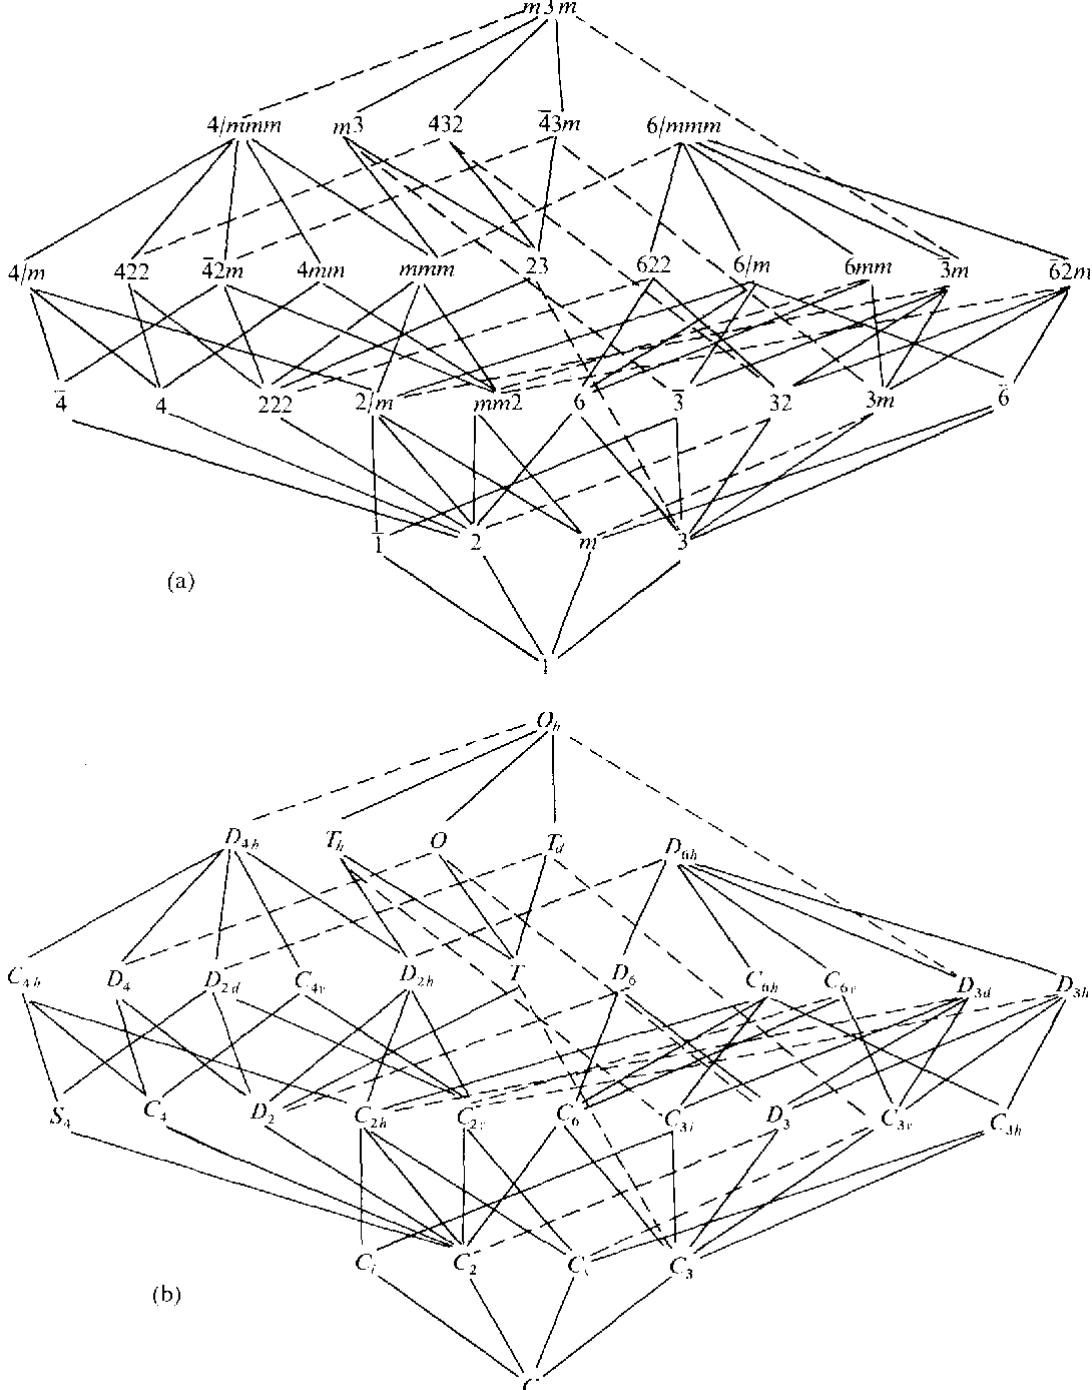
\includegraphics[width=0.66\textwidth]{fig4_1_mu.jpg}
\caption*{\textbf{图 4.1}\ 点群之间的谱系关系。实线表示子群是不变的：(a) 国际记号；(b) Schönflies 记号。}
\end{figure}

现在很容易对所有点群作出半直积，Altmann (1963\textit{a}, \textit{b}) 已考虑过这一问题。我们将把讨论限制在非循环的真转动群上，这是因为其余点群或者是循环群，或者同构于真转动群，或者是直积。表 4.1 以半直积的形式给出点群及其极大不变子群。

\begin{figure}[H]
\centering
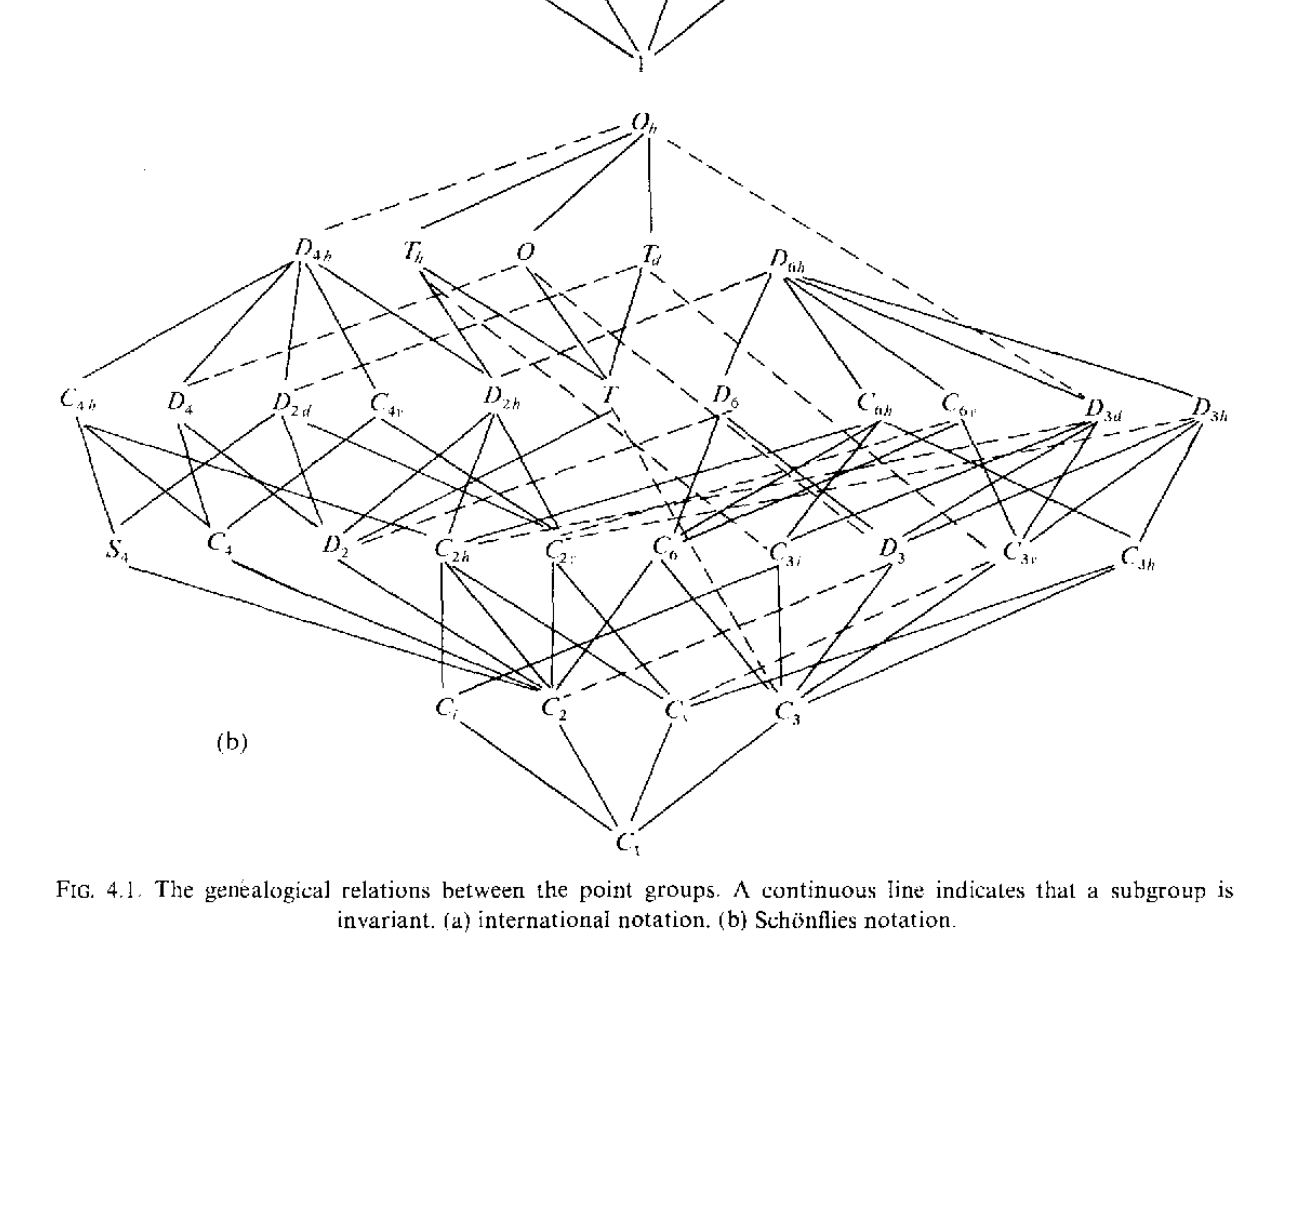
\includegraphics[width=0.88\textwidth]{c4_t41_p1.png}
\caption*{\textbf{表 4.1}\ 作为半直积的点群（原书扫描占位）。}
\end{figure}

表 4.1 的注（译文）：

\noindent（i）表的每一行中，依次给出一个群、它的极大不变子群以及相应的半直积。由大括号相连的两行中，第二行是第一行的 Schönflies 版本，符合我们同时给出两种记号的惯例。

\noindent（ii）群名上的撇号表示非标准定向。为获得完整的理解，读者应当用表 2.2 确定表中出现的所有群与子群的元素名称。

\noindent（iii）对 $222\ (D_{2})$，半直积表达式实际上是直积。

\noindent（iv）对 $432\ (O)$，其极大不变子群不是 Abel 群（与其他所有情形不同）。不过，也存在一个不变子群为 Abel 群的表达式，虽然该子群不是极大的，但分解中的另一因子此时是非循环的。

现在举一个例子，说明如何用不变子群的表示来确定半直积群的表示。考虑的情形是 $422 = 4 \wedge 2'\ (D_{4} = C_{4} \wedge C'_{2})$。一个合适的分解是
\begin{equation*}
\begin{array}{l}
422 = E.4 + C_{2x}.4\\
\left(D_{4} = E.C_{4} + C_{2x}.C_{4}\right).
\end{array}
\tag{4.5.1}
\end{equation*}
由表 2.2 可见 $4\ (C_{4})$ 的表示是四个一维表示 $A$、$B$、${}^{1}E$ 和 ${}^{2}E$，其中 $C^{+}_{4z}$ 分别由 $1$、$-1$、$-i$ 和 $i$ 表示。确立 $4\ (C_{4})$ 为不变子群的共轭关系是
\begin{center}
$C^{-1}_{2x}EC_{2x} = E$，\quad $C^{-1}_{2x}C^{+}_{4z}C_{2x} = C^{-}_{4z}$，\quad $C^{-1}_{2x}C_{2z}C_{2x} = C_{2z}$，\quad 以及 $C^{-1}_{2x}C^{-}_{4z}C_{2x} = C^{+}_{4z}$。
\end{center}
$4\ (C_{4})$ 的表示分成三颗星：单由 $A$ 组成的、单由 $B$ 组成的、以及由 ${}^{1}E$ 与 ${}^{2}E$ 合起来组成的。${}^{1}E$ 与 ${}^{2}E$ 走到一起，源于形如 ${}^{1}\mathbf{E}(C^{-1}_{2x}C^{+}_{4z}C_{2x}) = {}^{1}\mathbf{E}(C^{-}_{4z}) = {}^{2}\mathbf{E}(C^{+}_{4z})$ 的方程。

三种情形下的小陪群是：对星 $A$ 和 $B$，是含 $E$ 与 $C_{2x}$ 的群 $2'\ (C'_{2})$；对其余的星 $E$，是群 $1\ (C_{1})$。由于这是半直积，小陪群所需的表示就是它们的普通表示，这些可以从表 2.2 得到。

设 $\phi$ 是 ${}^{1}E$ 的基函数，于是
\begin{equation*}
C^{+}_{4z}\phi = \phi\,{}^{1}\mathbf{E}(C^{+}_{4z}) = -\mathrm{i}\phi.
\tag{4.5.2}
\end{equation*}
记 $C_{2x}\phi = \psi$，则 $\langle \phi, \psi |$ 是表示 ${}^{1}E \uparrow 422\ (D_{4}) = \Delta$ 的一个基。我们计算 $C^{+}_{4z}$ 与 $C_{2x}$ 的诱导矩阵表示。现在
\begin{equation*}
C^{+}_{4z}\psi = C^{+}_{4z}C_{2x}\phi = C_{2x}C^{-}_{4z}\phi = C_{2x}\phi\,{}^{1}\mathbf{E}(C^{-}_{4z}) = i\psi.
\tag{4.5.3}
\end{equation*}
由式 (4.5.2) 与 (4.5.3) 可见
\begin{equation*}
C^{+}_{4z}\langle \phi, \psi | = \langle -\mathrm{i}\phi, \mathrm{i}\psi | = \langle \phi, \psi |\begin{pmatrix} -\mathrm{i} & 0\\ 0 & \mathrm{i} \end{pmatrix}
\end{equation*}
因此
\begin{equation*}
\boldsymbol{\Delta}(C^{+}_{4z}) = \begin{pmatrix} -\mathrm{i} & 0\\ 0 & \mathrm{i} \end{pmatrix}.
\tag{4.5.4}
\end{equation*}
另外，按定义
\begin{equation*}
C_{2x}\phi = \psi
\tag{4.5.5}
\end{equation*}
于是
\begin{equation*}
C_{2x}\psi = C_{2x}C_{2x}\phi = \phi,
\tag{4.5.6}
\end{equation*}
从而
\begin{equation*}
\Delta(C_{2x}) = \begin{pmatrix} 0 & 1\\ 1 & 0 \end{pmatrix}.
\tag{4.5.7}
\end{equation*}
上述结果汇总于表 4.2；为了与表 2.2 一致，我们作认同 $\Lambda^{A}_{1} = A_{1}$、$\Lambda^{A}_{2} = A_{2}$、$\Lambda^{B}_{1} = B_{1}$、$\Lambda^{B}_{2} = B_{2}$、$\Delta = E$。

\begin{table}[H]
\centering
\caption*{\textbf{表 4.2}\ $422\ (D_{4})$ 的表示与 $4\ (C_{4})$ 的表示的关系（Altmann 1963\textit{a}）}
\begin{tabular}{@{}lllllllllllll@{}}
\toprule
$4\ (C_{4})$ & 星 & 小陪群 & $E$ & $C^{+}_{4z}$ & $C_{2z}$ & $C^{-}_{4z}$ & $422\ (D_{4})$ & $E$ & $C^{+}_{4z}$ & $C_{2z}$ & $C_{2x}$ & $C_{2a}$\\
 & & & & & & & & & $C^{-}_{4z}$ & & $C_{2y}$ & $C_{2b}$\\
\midrule
$A$ & $A$ & $2'\ (C'_{2})$ & 1 & 1 & 1 & 1 & $A_{1}$ & 1 & 1 & 1 & 1 & 1\\
 & & & & & & & $A_{2}$ & 1 & 1 & 1 & $-1$ & $-1$\\
$B$ & $B$ & $2'\ (C'_{2})$ & 1 & $-1$ & 1 & $-1$ & $B_{1}$ & 1 & $-1$ & 1 & 1 & $-1$\\
 & & & & & & & $B_{2}$ & 1 & $-1$ & 1 & $-1$ & 1\\
${}^{1}E$ & $E$ & $1\ (C_{1})$ & $\begin{cases}1\\ 1\end{cases}$ & $\begin{cases}-i\\ i\end{cases}$ & $\begin{cases}-1\\ -1\end{cases}$ & $\begin{cases}i\\ -i\end{cases}$ & $E$ & 2 & 0 & $-2$ & 0 & 0\\
${}^{2}E$ & & & & & & & & & & & &\\
\bottomrule
\end{tabular}
\end{table}

表 4.3 复制了表 4.1 中出现的其余半直积的类似关系的汇总（原书扫描占位）。

\begin{figure}[H]
\centering
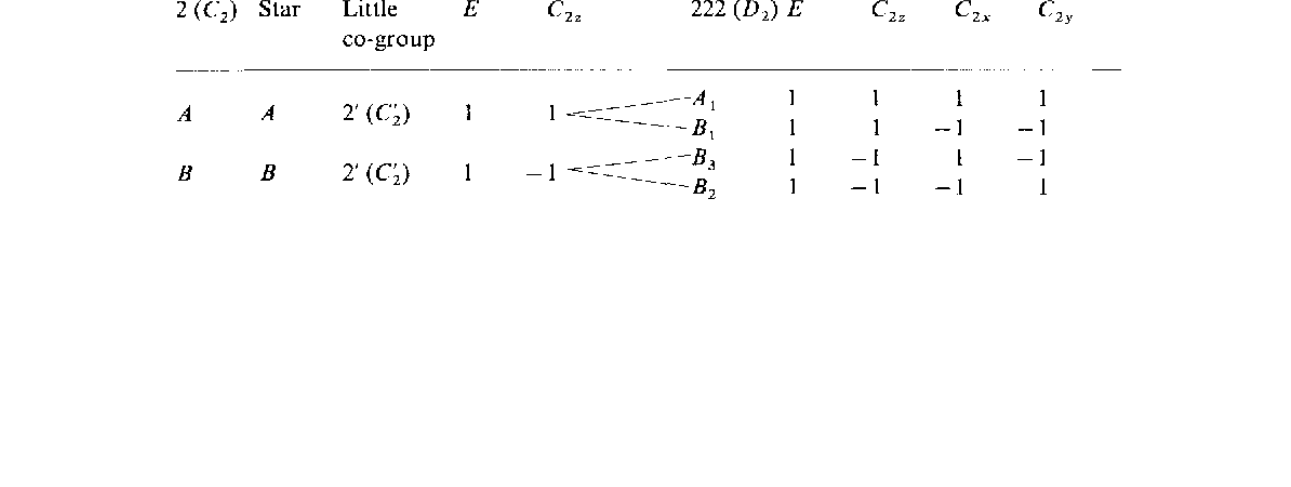
\includegraphics[width=0.92\textwidth]{c4_t43_p1.png}
\caption*{\textbf{表 4.3}\ 点群的表示与其不变子群的表示的关系（Altmann 1963\textit{a}；原书扫描占位）。}
\end{figure}
\begin{figure}[H]
\centering
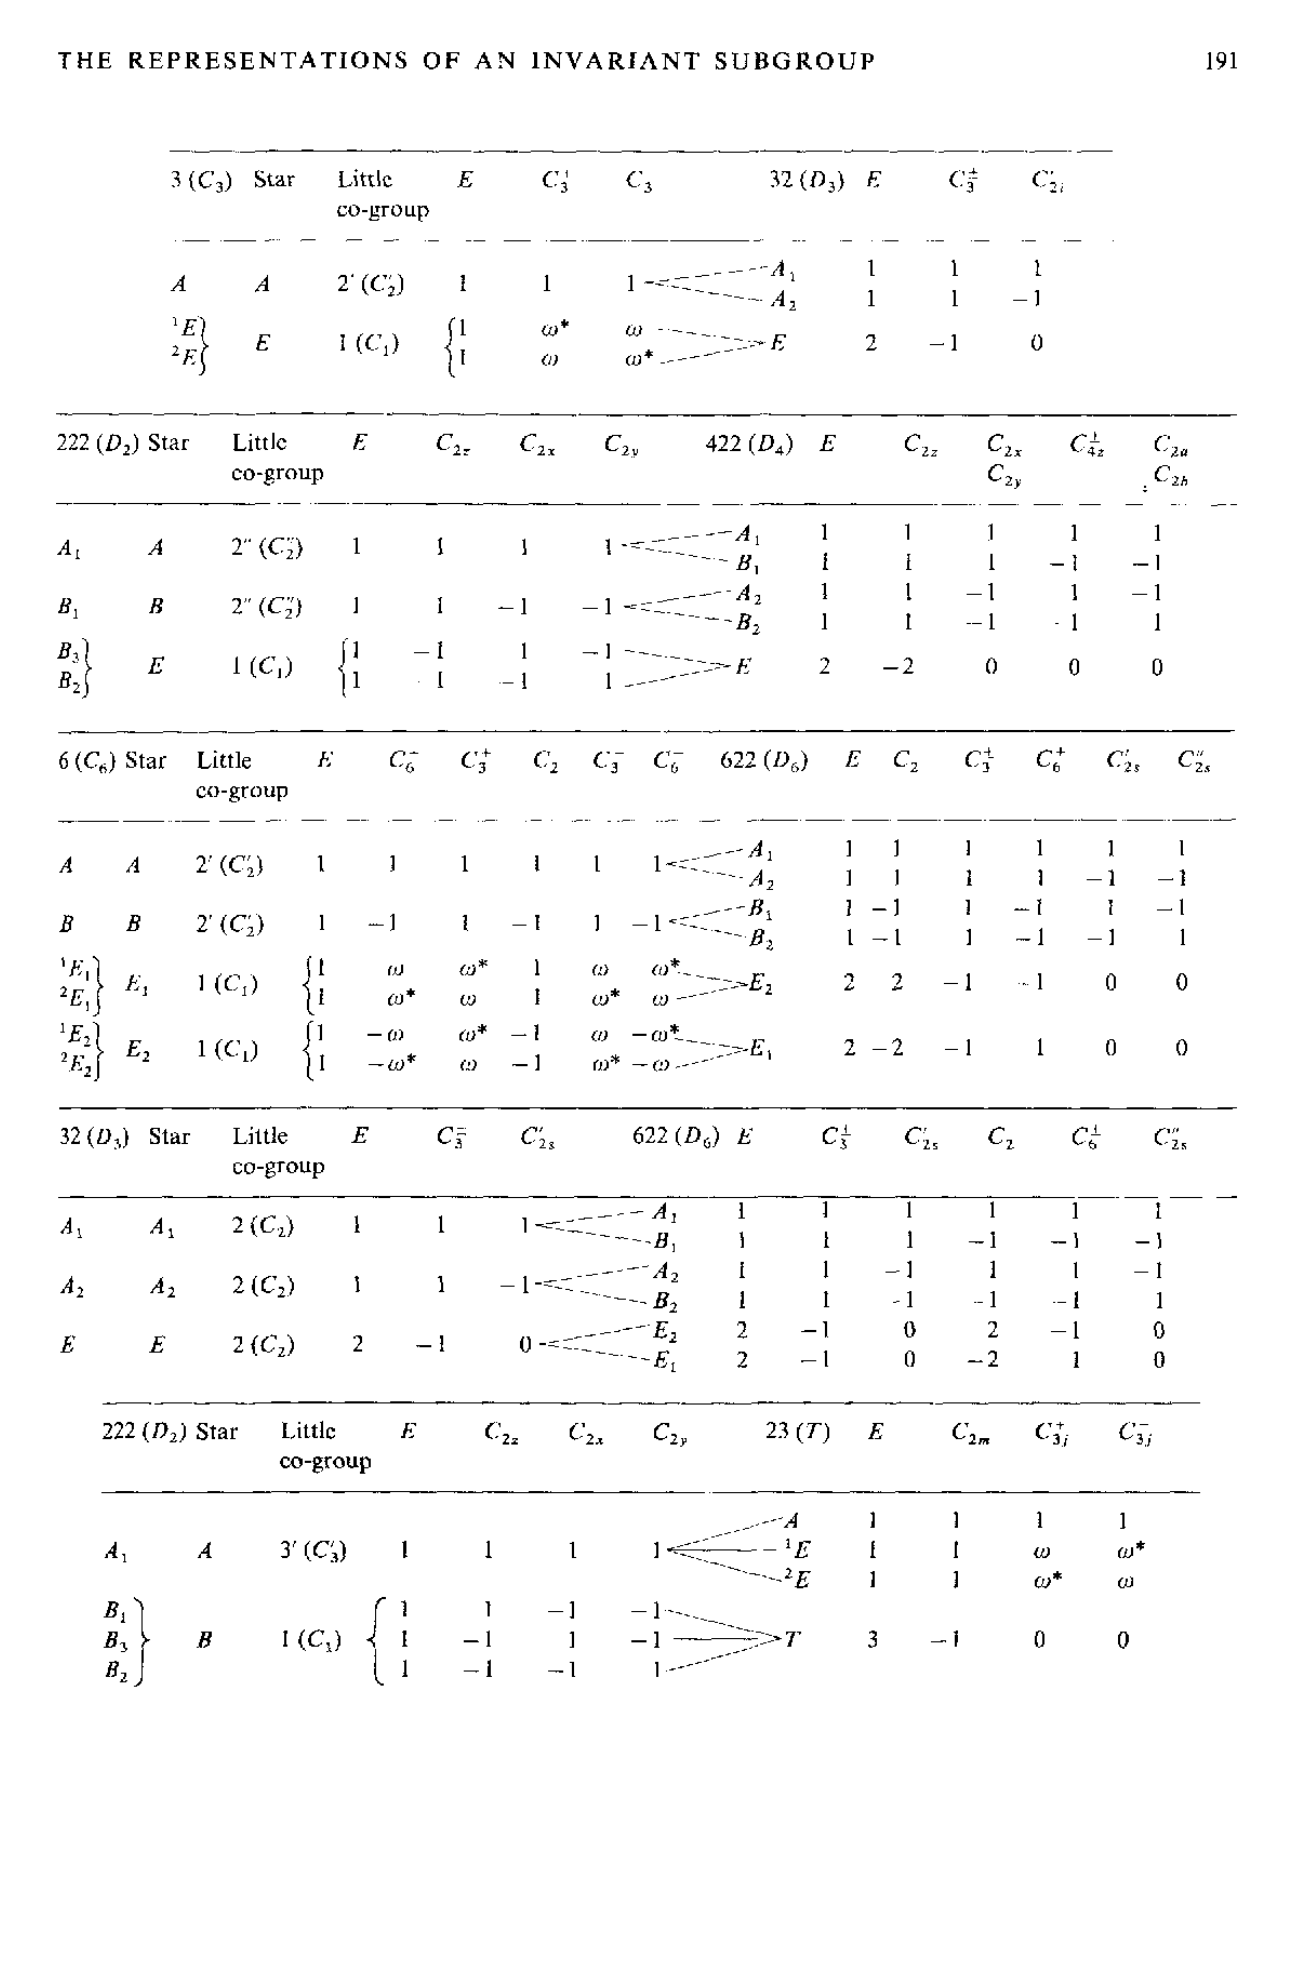
\includegraphics[width=0.92\textwidth]{c4_t43_p2.png}
\caption*{\textbf{表 4.3}（第 2 页）。}
\end{figure}
\begin{figure}[H]
\centering
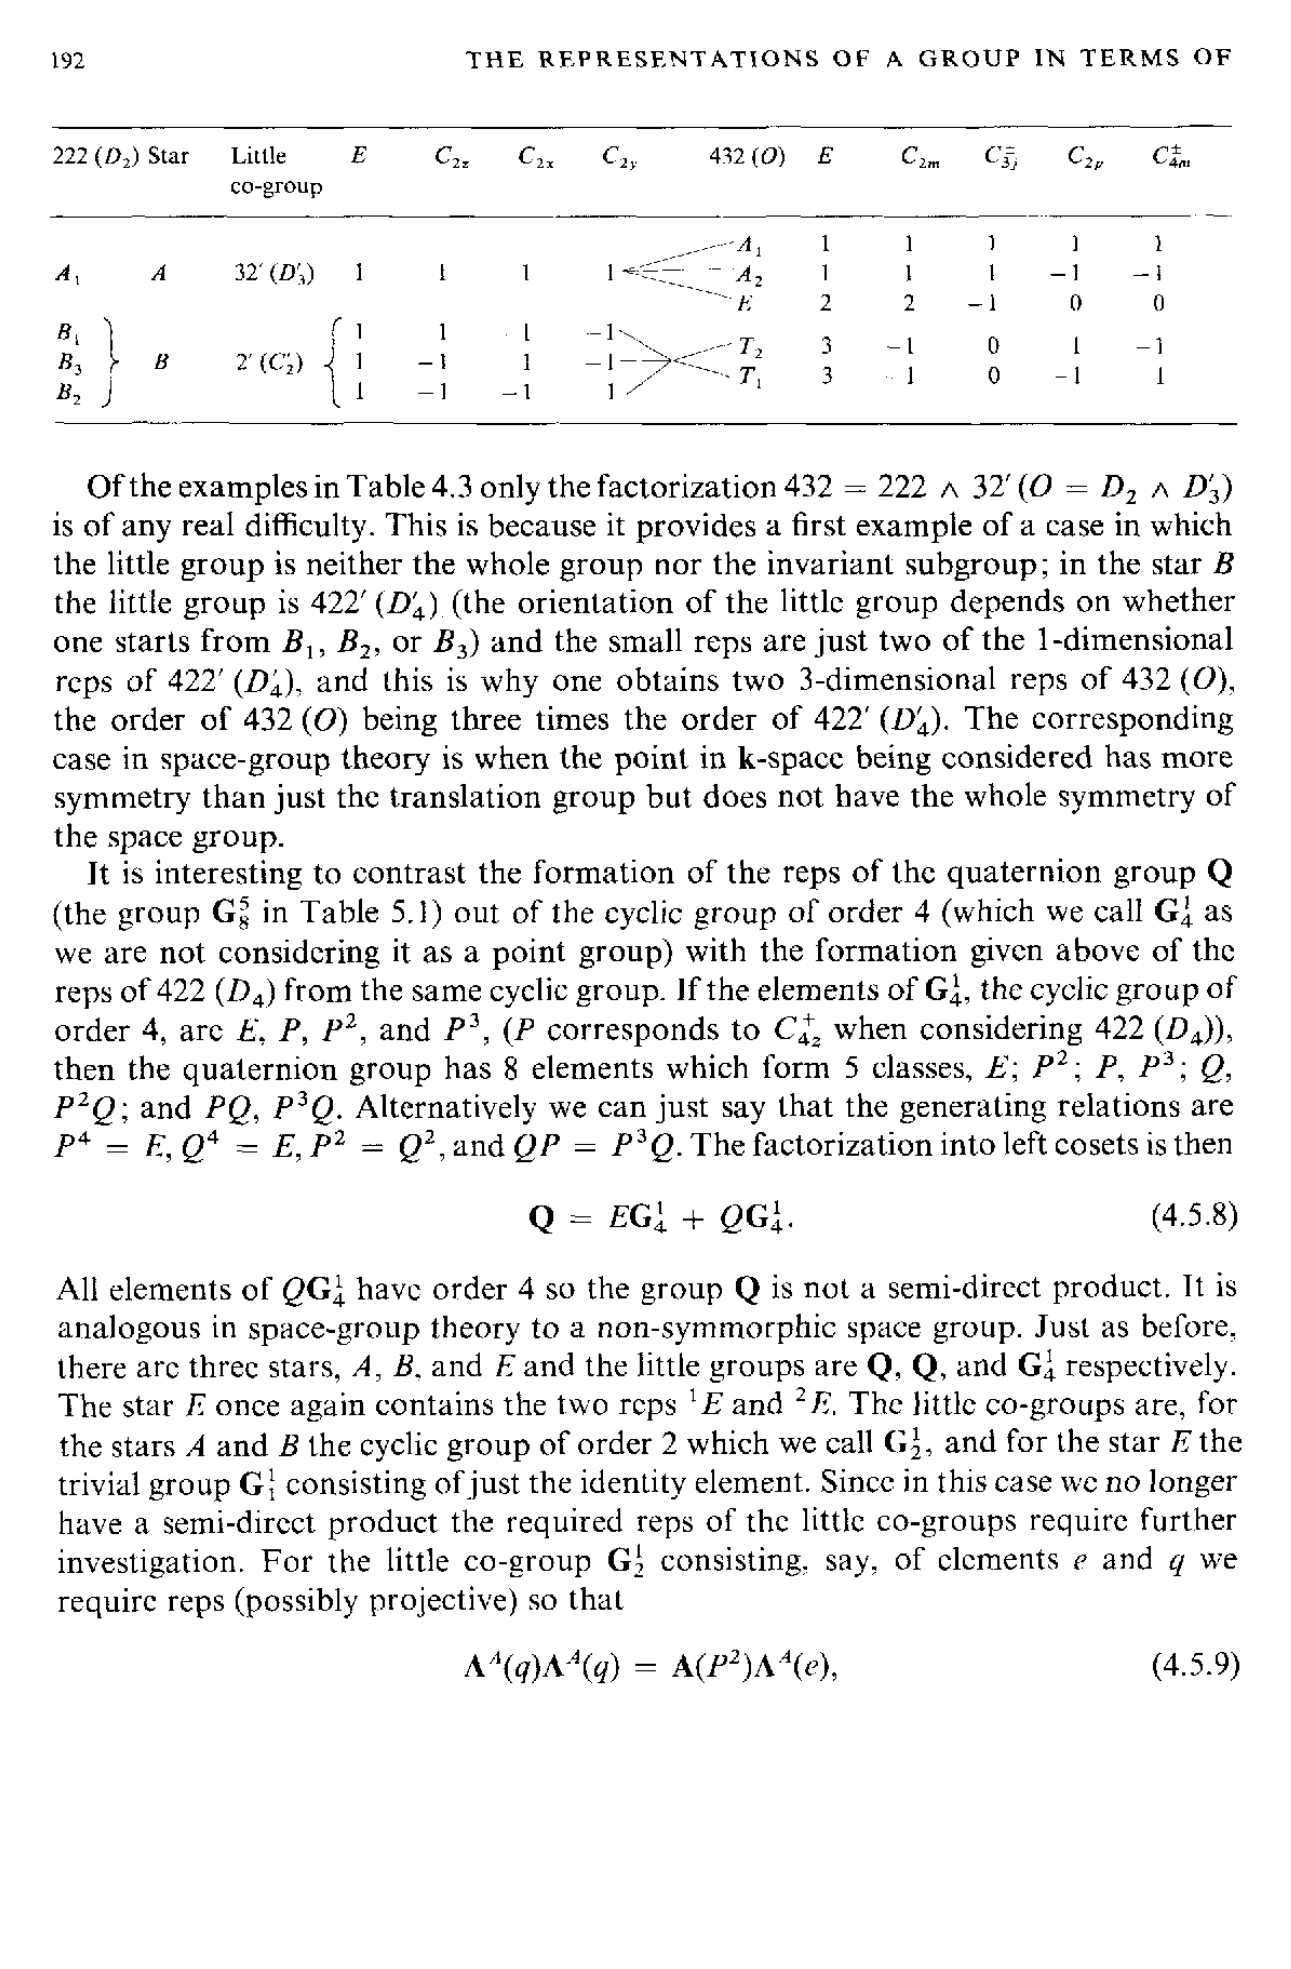
\includegraphics[width=0.92\textwidth]{c4_t43_p3.png}
\caption*{\textbf{表 4.3}（第 3 页）。}
\end{figure}
\begin{figure}[H]
\centering
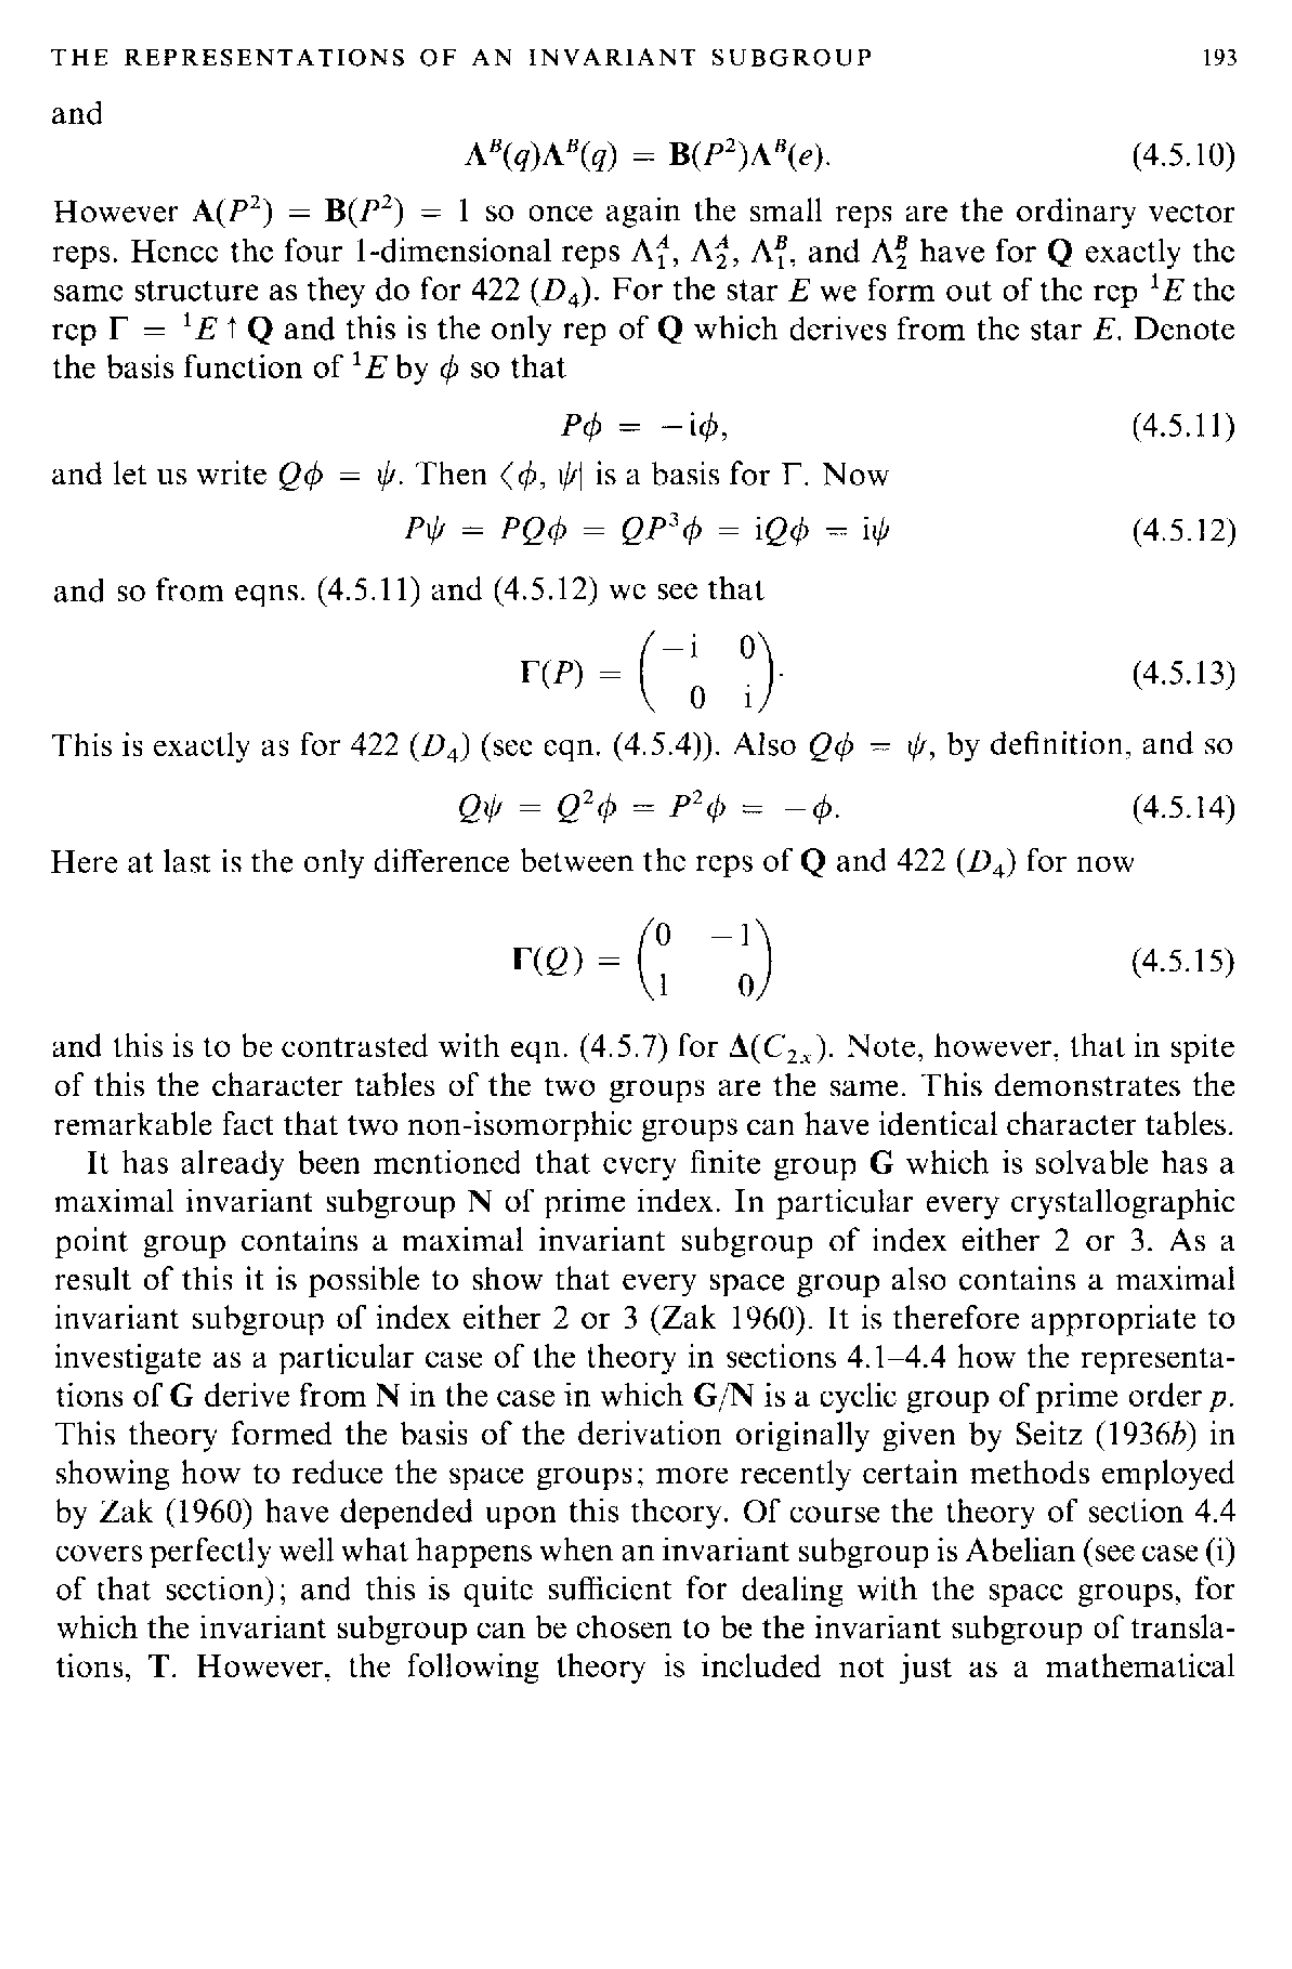
\includegraphics[width=0.92\textwidth]{c4_t43_p4.png}
\caption*{\textbf{表 4.3}（第 4 页）。}
\end{figure}

在表 4.3 的例子中，只有分解 $432 = 222 \wedge 32'\ (O = D_{2} \wedge D'_{3})$ 真正有些困难。因为它提供了这样一个例子：小群既不是整个群也不是不变子群。在星 $B$ 中，小群是 $422'\ (D'_{4})$（小群的取向依赖于从 $B_{1}$、$B_{2}$ 还是 $B_{3}$ 出发），而小表示恰是 $422'\ (D'_{4})$ 的两个一维表示；这就是为什么我们得到 $432\ (O)$ 的两个三维表示——$432\ (O)$ 的阶是 $422'\ (D'_{4})$ 阶的三倍。空间群理论中相应的情形是：所考虑的 $\mathbf{k}$ 空间的点具有比平移群更多的对称性，但又不具有空间群的全部对称性。

有趣的是，把四元数群 $\mathbf{Q}$（表 5.1 中的群 $\mathbf{G}^{5}_{8}$）的表示——由 4 阶循环群（由于不把它当作点群，记作 $\mathbf{G}^{1}_{4}$）出发构成——的生成方式，与上面从同一个循环群生成 $422\ (D_{4})$ 的表示的方式加以对比。设 $\mathbf{G}^{1}_{4}$（4 阶循环群）的元素是 $E, P, P^{2}, P^{3}$（考虑 $422\ (D_{4})$ 时 $P$ 对应于 $C^{+}_{4z}$），则四元数群有 8 个元素，分为 5 个类：$E$；$P^{2}$；$P, P^{3}$；$Q, P^{2}Q$；以及 $PQ, P^{3}Q$。也可以直接说生成关系是 $P^{4} = E$、$Q^{4} = E$、$P^{2} = Q^{2}$、$QP = P^{3}Q$。左陪集分解为
\begin{equation*}
\mathbf{Q} = E\mathbf{G}^{1}_{4} + Q\mathbf{G}^{1}_{4}.
\tag{4.5.8}
\end{equation*}
$Q\mathbf{G}^{1}_{4}$ 的所有元素都是 4 阶的，所以群 $\mathbf{Q}$ 不是半直积。它在空间群理论中类似于一个非点式空间群。与之前一样，这里有三颗星 $A$、$B$ 和 $E$，小群分别是 $\mathbf{Q}$、$\mathbf{Q}$ 和 $\mathbf{G}^{1}_{4}$。星 $E$ 同样包含两个表示 ${}^{1}E$ 与 ${}^{2}E$。小陪群是：对星 $A$ 和 $B$，是我们记作 $\mathbf{G}^{1}_{2}$ 的 2 阶循环群；对星 $E$，是仅由恒等元组成的平凡群 $\mathbf{G}^{1}_{1}$。由于此情形不再是半直积，小陪群所需的表示需要进一步考察。对由元素 $e$ 与 $q$ 组成的小陪群 $\mathbf{G}^{1}_{2}$，我们需要（可能是射影的）表示使得
\begin{equation*}
\boldsymbol{\Lambda}^{A}(q)\boldsymbol{\Lambda}^{A}(q) = \mathbf{A}(P^{2})\boldsymbol{\Lambda}^{A}(e),
\tag{4.5.9}
\end{equation*}
以及
\begin{equation*}
\boldsymbol{\Lambda}^{B}(q)\boldsymbol{\Lambda}^{B}(q) = \mathbf{B}(P^{2})\boldsymbol{\Lambda}^{B}(e).
\tag{4.5.10}
\end{equation*}
然而 $\mathbf{A}(P^{2}) = \mathbf{B}(P^{2}) = 1$，所以小表示再一次是普通矢量表示。于是四个一维表示 $\Lambda^{A}_{1}, \Lambda^{A}_{2}, \Lambda^{B}_{1}, \Lambda^{B}_{2}$ 对 $\mathbf{Q}$ 具有与对 $422\ (D_{4})$ 完全相同的结构。对星 $E$，我们从表示 ${}^{1}E$ 构造表示 $\Gamma = {}^{1}E \uparrow \mathbf{Q}$，这是从星 $E$ 得到的 $\mathbf{Q}$ 的唯一表示。记 ${}^{1}E$ 的基函数为 $\phi$，使得
\begin{equation*}
P\phi = -\mathrm{i}\phi,
\tag{4.5.11}
\end{equation*}
并记 $Q\phi = \psi$，则 $\langle \phi, \psi |$ 是 $\Gamma$ 的一个基。现在
\begin{equation*}
P\psi = PQ\phi = QP^{3}\phi = \mathrm{i}Q\phi = \mathrm{i}\psi
\tag{4.5.12}
\end{equation*}
于是由式 (4.5.11) 与 (4.5.12) 可见
\begin{equation*}
\Gamma(P) = \begin{pmatrix} -\mathrm{i} & 0\\ 0 & \mathrm{i} \end{pmatrix}.
\tag{4.5.13}
\end{equation*}
这与 $422\ (D_{4})$ 的情形完全一样（见式 (4.5.4)）。另外 $Q\phi = \psi$（按定义），于是
\begin{equation*}
Q\psi = Q^{2}\phi = P^{2}\phi = -\phi.
\tag{4.5.14}
\end{equation*}
这里终于出现了 $\mathbf{Q}$ 与 $422\ (D_{4})$ 的表示之间的唯一差别：现在
\begin{equation*}
\boldsymbol{\Gamma}(Q) = \begin{pmatrix} 0 & -1\\ 1 & 0 \end{pmatrix}
\tag{4.5.15}
\end{equation*}
这与 $\Delta(C_{2x})$ 的式 (4.5.7) 形成对照。但尽管如此，两个群的特征标表是相同的。这展示了一个显著的事实：两个不同构的群可以有完全相同的特征标表。

前面已经提到，每个可解的有限群 $\mathbf{G}$ 都有素数指数的极大不变子群 $\mathbf{N}$。特别地，每个晶体学点群都含有一个指数为 2 或 3 的极大不变子群。由此可以证明每个空间群也含有指数为 2 或 3 的极大不变子群（Zak 1960）。因此，作为 4.1--4.4 节理论的特殊情形，考察当 $\mathbf{G}/\mathbf{N}$ 是素数 $p$ 阶循环群时 $\mathbf{G}$ 的表示如何从 $\mathbf{N}$ 的表示导出，是合适的。这一理论构成了 Seitz (1936\textit{b}) 原本给出的、说明如何约化空间群的基础；近年 Zak (1960) 采用的某些方法也依赖于此理论。当然，4.4 节的理论对不变子群为 Abel 群的情形（见该节情形 (i)）已覆盖得很好；这对空间群已相当足够，因为其不变子群可取为平移不变子群 $\mathbf{T}$。然而下面包括的理论不仅仅作为数学练习，也不仅仅由于其历史意义，而是因为它进一步揭示了我们处理的这些群的结构。例如，它说明了如何利用像 $432 = 23 \wedge 2''\ (O = T \wedge C''_{2})$（见表 4.1）这样的分解——由于 $23\ (T)$ 不是 Abel 群，它不落在 4.4 节情形 (i) 的范围内。附带地，该理论表明当 $\mathbf{G}/\mathbf{N}$ 为素数阶时，4.4 节的情形 (ii) 并不像乍看之下那样难于处理。

设 $\mathbf{G}$ 是群，$\mathbf{N}$ 是 $\mathbf{G}$ 的素数指数 $p$ 的极大不变子群。此时可以把 $\mathbf{G}$ 分解成左陪集
\begin{equation*}
\mathbf{G} = \mathbf{N} + r\mathbf{N} + r^{2}\mathbf{N} + \dots + r^{p-1}\mathbf{N}
\tag{4.5.16}
\end{equation*}
其中 $r^{p} \in \mathbf{N}$。当 $r^{p}$ 等于恒等元 $E$ 时，$\mathbf{G}$ 是 $\mathbf{N}$ 与 $p$ 阶循环群的半直积。更一般地，设 $r^{p} = \bar{n} \in \mathbf{N}$ 且 $\bar{n}$ 的阶为 $l$。则 $E = \bar{n}^{l} = r^{lp}$。若 $1 \leqslant l \leqslant p$，则由于 $p$ 是素数，可以选 $s = r^{l}$ 代替 $r$，组成另一种陪集分解
\begin{equation*}
\mathbf{G} = \mathbf{N} + s\mathbf{N} + s^{2}\mathbf{N} + \dots + s^{p-1}\mathbf{N}
\tag{4.5.17}
\end{equation*}
此时 $s^{p} = E$。于是取上述范围内的 $l$ 值，就可以重新选取 $r$ 使 $l = 1$。另一方面，若 $l = p$，则不存在这种替代选择。沿这些路线的进一步论证表明，总可以这样选取 $r$，使得 $l$ 取 $p$ 的幂值，即 $l = 1, p, p^{2}, \dots$。因此在分解 (4.5.16) 中可以不失一般性地假定 $r^{(p^{m})} = E$，其中 $m \geqslant 1$。

接下来考察 $\mathbf{G}$ 相对于 $\mathbf{N}$ 的类结构。设 $C_{1}, C_{2}, \dots, C_{n}$ 是 $\mathbf{N}$ 的类。可以证明用 $r$ 作共轭会给出这些类的一个置换。设 $n_{i} \in C_{i}$ 且 $rn_{i}r^{-1} = n_{j} \in C_{j}$。设 $n'_{i}$ 是 $C_{i}$ 的任一其他元素，则存在 $n \in \mathbf{N}$ 使 $n'_{i} = nn_{i}n^{-1}$，且 $rn'_{i}r^{-1} = rnn_{i}n^{-1}r^{-1}$。由于 $\mathbf{N}$ 在 $\mathbf{G}$ 中不变，存在 $n' \in \mathbf{N}$ 使 $rn = n'r$。于是 $rn'_{i}r^{-1} = n'(rn_{i}r^{-1})n'^{-1} = n'n_{j}n'^{-1} \in C_{j}$。这表明 $rC_{i}r^{-1} \subseteq C_{j}$，从而 $C_{i}$ 的元素数 $s_{i}$ 小于或等于 $C_{j}$ 的元素数 $s_{j}$。用 $r^{-1}$ 作共轭的类似论证给出 $r^{-1}C_{j}r \subseteq C_{i}$ 且 $s_{j} \leqslant s_{i}$。因此 $rC_{i}r^{-1} = C_{j}$ 且 $s_{i} = s_{j}$。设 $C_{k}$ 是另一个使 $rC_{k}r^{-1} = C_{j}$ 的类，则 $C_{i} = r^{-1}C_{j}r = C_{k}$。故用 $r$ 作共轭产生 $\mathbf{N}$ 的类上的一个置换 $\pi(r)$。类似地可以证明，用 $r^{m}$ 作共轭产生 $\mathbf{N}$ 的类上的置换 $\pi(r^{m})$（$m = 1, 2, \dots p$）。由于 $r^{p} \in \mathbf{N}$，$\pi(r^{p})$ 是恒等置换 $\varepsilon$。又有 $\{\pi(r)\}^{2}C_{i} = \pi(r)rC_{i}r^{-1} = r^{2}C_{i}r^{-2} = \pi(r^{2})C_{i}$，故 $\{\pi(r)\}^{2} = \pi(r^{2})$，类似地 $\{\pi(r)\}^{m} = \pi(r^{m})$。于是 $\{\pi(r)\}^{p} = \pi(r^{p}) = \varepsilon$。因此 $\pi(r)$ 的阶整除 $p$。由于 $p$ 是素数，$\pi(r)$ 的阶为 1 或 $p$。这意味着把 $\pi(r)$ 分解为不相交循环的乘积时，任何循环的长度是 1 或 $p$。所以 $\mathbf{N}$ 的类有两种：在 $r$ 下自共轭的类（$rC_{i}r^{-1} = C_{i}$），以及以长度为 $p$ 的循环出现、使 $C_{i}, rC_{i}r^{-1}, r^{2}C_{i}r^{-2}, \dots, r^{p-1}C_{i}r^{-(p-1)}$ 构成 $\mathbf{N}$ 的 $p$ 个不同类的那些类。于是 $\mathbf{G}$ 相对于 $\mathbf{N}$ 的类结构确定如下：$\mathbf{N}$ 在 $r$ 下自共轭的类也是 $\mathbf{G}$ 的类；不自共轭的类与 $(p-1)$ 个其他类按上述方式联合，构成 $\mathbf{G}$ 的一个单独的类。

下面说明如何由 $\mathbf{N}$ 的表示确定 $\mathbf{G}$ 的表示。设 $\Delta_{0}$ 是 $\mathbf{N}$ 的维数为 $d$ 的表示，$\phi_{0i}$（$i = 1$ 到 $d$）是 $\Delta_{0}$ 的基，使得对一切 $n \in \mathbf{N}$
\begin{equation*}
n\phi_{0i} = \sum^{d}_{j=1}\phi_{0j}\Delta_{0}(n)_{ji}
\tag{4.5.18}
\end{equation*}
（$i = 1, 2, \dots, d$）。与 4.1 节同样地定义函数
\begin{equation*}
\phi_{mi} = r^{m}\phi_{0i}
\tag{4.5.19}
\end{equation*}
（$m = 0, 1, \dots, (p-1)$，$i = 1, 2, \dots, d$），则类比式 (4.2.16) 可知，对固定的 $m$
\begin{equation*}
n\phi_{mi} = \sum^{d}_{j=1}\phi_{mj}\Delta_{0}(r^{-m}nr^{m})_{ji}
\tag{4.5.20}
\end{equation*}
（$i = 1, 2, \dots, d$）。由 4.2 节的理论可见，这样我们定义了 $\mathbf{N}$ 的 $p$ 个表示 $\Delta_{m}$：
\begin{equation*}
\Delta_{m}(n) = \Delta_{0}(r^{-m}nr^{m})
\tag{4.5.21}
\end{equation*}
（$m = 0, 1, \dots, (p-1)$）。现在 $\mathbf{G}/\mathbf{N}$ 同构于 $p$ 阶循环群 $C_{p}$。由于 $p$ 是素数，只能出现两种情形。$\Delta_{0}$ 的小陪群的阶是 $|\mathbf{G}/\mathbf{N}|$ 的因子，必为 1 或 $p$；$\Delta_{0}$ 的星相应地分别含 $p$ 个表示或 1 个表示。于是得到与类结构类似的结果：要么 $\Delta_{0}$ 在 $r$ 下自共轭、诸 $\Delta_{m}$ 彼此等价、小群是整个群 $\mathbf{G}$；要么诸 $\Delta_{m}$ 彼此不等价、小群恰为不变子群 $\mathbf{N}$。

\noindent\textbf{情形 (i)}\ 设 $\Delta_{m}$（$m = 0, 1, \dots, (p-1)$）彼此不等价。则由 4.2 节的理论立即可知 $\Delta_{0} \uparrow \mathbf{G}$ 不可约。$\Delta_{0} \uparrow \mathbf{G}$ 的特征标由式 (4.2.22) 立刻得到：
\begin{equation*}
\chi_{\Delta_{0} \uparrow \mathbf{G}}(n) = \sum^{p-1}_{m=0}\chi_{\Delta_{0}}(r^{-m}nr^{m}) = \sum^{p-1}_{m=0}\chi_{\Delta_{m}}(n)
\tag{4.5.22}
\end{equation*}
以及
\begin{equation*}
\chi_{\Delta_{0} \uparrow \mathbf{G}}(r^{i}n) = 0
\tag{4.5.23}
\end{equation*}
（$i = 1, 2, \dots, (p-1)$）。

\noindent\textbf{情形 (ii)}\ 设 $\Delta_{m}$（$m = 0, 1, \dots, (p-1)$）彼此等价。则 $\Delta_{0} \uparrow \mathbf{G}$ 可约。由于诸 $\Delta_{m}$ 有相同的特征标，$\Delta_{0} \uparrow \mathbf{G}$ 的特征标由
\begin{equation*}
\chi_{\Delta_{0} \uparrow \mathbf{G}}(n) = p\chi_{\Delta_{0}}(n)
\tag{4.5.24}
\end{equation*}
以及
\begin{equation*}
\chi_{\Delta_{0} \uparrow \mathbf{G}}(r^{i}n) = 0
\tag{4.5.25}
\end{equation*}
（$i = 1, 2, \dots, (p-1)$）给出。于是 $\Delta_{0} \uparrow \mathbf{G}$ 与自身的交织数为
\begin{equation*}
\frac{1}{|\mathbf{G}|}\sum_{g \in \mathbf{G}}\left|\chi_{\Delta_{0} \uparrow \mathbf{G}}(g)\right|^{2} = \frac{1}{|\mathbf{G}|}p^{2}\sum_{n \in \mathbf{N}}\left|\chi_{\Delta_{0}}(n)\right|^{2} = p^{2}|\mathbf{N}|/|\mathbf{G}| = p.
\tag{4.5.26}
\end{equation*}
因此可以想见，此情形下 $\Delta_{0} \uparrow \mathbf{G}$ 可约化为 $p$ 个彼此不等价的 $\mathbf{G}$ 的表示，每个维数为 $d$。下面我们证明确实如此，并特别说明如何实现约化以及如何得到各分表示的特征标。由于 $\mathbf{G}$ 的每个元素都可写成 $r^{i}n$（$i$ 在 0 到 $(p-1)$ 之间，$n \in \mathbf{N}$），为了约化 $\Delta_{0} \uparrow \mathbf{G}$，只需找一个基变换，把 $n$ 与 $r$ 的代表矩阵同时约化到相同的块对角形式。相对于基 $\langle \phi_{0i}, \phi_{1i}, \dots, \phi_{(p-1)i} |$，$n$ 的代表显然是
\begin{equation*}
(\Delta_{0} \uparrow \mathbf{G})(n) = \begin{pmatrix} \Delta_{0}(n) & 0 & 0 & \dots & 0\\ 0 & \Delta_{0}(r^{-1}nr) & 0 & \dots & 0\\ 0 & 0 & \Delta_{0}(r^{-2}nr^{2}) & \dots & 0\\ \vdots & \vdots & \vdots & & \vdots\\ 0 & 0 & 0 & \dots & \Delta_{0}(r^{-p+1}nr^{p-1}) \end{pmatrix}
\tag{4.5.27}
\end{equation*}
又由于 $\phi_{mi} = r^{m}\phi_{0i}$，
\begin{equation*}
\begin{aligned}
r\langle \phi_{0i}, \phi_{1i}, \dots, \phi_{(p-1)i} | &= \langle r\phi_{0i}, r^{2}\phi_{0i}, \dots, r^{p}\phi_{0i} |\\
&= \langle \phi_{1i}, \phi_{2i}, \dots, \phi_{(p-1)i}, \sum_{j}\phi_{0j}\Delta_{0}(r^{p})_{ji} |
\end{aligned}
\tag{4.5.28}
\end{equation*}
其中在最后的分量中用了 $r^{p} \in \mathbf{N}$ 的事实。因此
\begin{equation*}
(\Delta_{0} \uparrow \mathbf{G})(r) = \begin{pmatrix} 0 & 0 & 0 & \dots & 0 & \Delta_{0}(r^{p})\\ \mathbf{1} & 0 & 0 & \dots & 0 & 0\\ 0 & \mathbf{1} & 0 & \dots & 0 & 0\\ \vdots & \vdots & \vdots & & \vdots & \vdots\\ 0 & 0 & 0 & \dots & \mathbf{1} & 0 \end{pmatrix}
\tag{4.5.29}
\end{equation*}
已知 $\Delta_{1}$ 与 $\Delta_{0}$ 等价，故存在幺正矩阵 $\mathbf{P}$ 使得对一切 $n \in \mathbf{N}$
\begin{equation*}
\Delta_{1}(n) = \mathbf{P}\Delta_{0}(n)\mathbf{P}^{-1}.
\tag{4.5.30}
\end{equation*}
于是 $\Delta_{2}(n) = \Delta_{0}(r^{-2}nr^{2}) = \Delta_{0}(r^{-1}n'r) = \Delta_{1}(n') = \mathbf{P}\Delta_{0}(n')\mathbf{P}^{-1} = \mathbf{P}\Delta_{0}(r^{-1}nr)\mathbf{P}^{-1} = \mathbf{P}^{2}\Delta_{0}(n)\mathbf{P}^{-2}$，更一般地用归纳法得
\begin{equation*}
\Delta_{m}(n) = \mathbf{P}^{m}\Delta_{0}(n)\mathbf{P}^{-m}
\tag{4.5.31}
\end{equation*}
（$m = 0, 1, 2, \dots, (p-1)$）。因此定义新基
\begin{equation*}
\psi_{mi} = \sum^{d}_{j=1}\phi_{mj}(\mathbf{P}^{m})_{ji}
\tag{4.5.32}
\end{equation*}
（$m = 0, 1, \dots, (p-1)$，$i = 1, 2, \dots, d$），则简短的计算表明，相对于这个新基
\begin{equation*}
(\Delta_{0} \uparrow \mathbf{G})(n) = \begin{pmatrix} \Delta_{0}(n) & 0 & 0 & \dots & 0\\ 0 & \Delta_{0}(n) & 0 & \dots & 0\\ 0 & 0 & \Delta_{0}(n) & \dots & 0\\ \vdots & \vdots & \vdots & & \vdots\\ 0 & 0 & 0 & \dots & \Delta_{0}(n) \end{pmatrix}
\tag{4.5.33}
\end{equation*}
以及
\begin{equation*}
(\Delta_{0} \uparrow \mathbf{G})(r) = \begin{pmatrix} 0 & 0 & 0 & \dots & 0 & \Delta_{0}(r^{p})\mathbf{P}^{p-1}\\ \mathbf{P}^{-1} & 0 & 0 & \dots & 0 & 0\\ 0 & \mathbf{P}^{-1} & 0 & \dots & 0 & 0\\ \vdots & \vdots & \vdots & & \vdots & \vdots\\ 0 & 0 & 0 & \dots & \mathbf{P}^{-1} & 0 \end{pmatrix}
\tag{4.5.34}
\end{equation*}
下一步证明 $\Delta_{0}(r^{p})\mathbf{P}^{p}$ 是单位矩阵的标量倍。设 $n$ 是 $\mathbf{N}$ 的任一元素，由于 $r^{p} \in \mathbf{N}$，
\begin{equation*}
\begin{aligned}
\Delta_{0}(n)\Delta_{0}(r^{p})\mathbf{P}^{p} &= \Delta_{0}(nr^{p})\mathbf{P}^{p} = \Delta_{0}(r^{p})\Delta_{0}(r^{-p}nr^{p})\mathbf{P}^{p}\\
&= \Delta_{0}(r^{p})\Delta_{1}(r^{-p+1}nr^{p-1})\mathbf{P}^{p} = \Delta_{0}(r^{p})\mathbf{P}\Delta_{0}(r^{-p+1}nr^{p-1})\mathbf{P}^{p-1}\\
&= \Delta_{0}(r^{p})\mathbf{P}^{p}\Delta_{0}(n),
\end{aligned}
\end{equation*}
（重复这一论证）。故 $\Delta_{0}(r^{p})\mathbf{P}^{p}$ 与 $\mathbf{N}$ 的表示 $\Delta_{0}$ 可交换，于是由 Schur 引理
\begin{equation*}
\Delta_{0}(r^{p})\mathbf{P}^{p} = \lambda\mathbf{1}
\tag{4.5.35}
\end{equation*}
其中 $\lambda$ 是一个相位因子。由式 (4.5.30) 可见矩阵 $\mathbf{P}$ 可以乘一个相位因子；特别地可以选取 $\mathbf{P}$ 使 $\lambda = 1$。假定已作了这一选择，并记 $\mathbf{P}^{-1} = \mathbf{R}$，则下列方程成立：
\begin{equation*}
\Delta_{1}(n) = \mathbf{R}^{-1}\Delta_{0}(n)\mathbf{R}
\tag{4.5.36}
\end{equation*}
\begin{equation*}
\Delta_{0}(r^{p}) = \mathbf{R}^{p}
\tag{4.5.37}
\end{equation*}
\begin{equation*}
(\Delta_{0} \uparrow \mathbf{G})(r) = \begin{pmatrix} 0 & 0 & 0 & \dots & 0 & \mathbf{R}\\ \mathbf{R} & 0 & 0 & \dots & 0 & 0\\ 0 & \mathbf{R} & 0 & \dots & 0 & 0\\ \vdots & \vdots & \vdots & & \vdots & \vdots\\ 0 & 0 & 0 & \dots & \mathbf{R} & 0 \end{pmatrix},
\tag{4.5.38}
\end{equation*}
且式 (4.5.33) 对 $(\Delta_{0} \uparrow \mathbf{G})(n)$ 依然成立。张成这个表示的基可以记作 $\langle \chi_{0}, \chi_{1}, \dots, \chi_{p-1} |$，其中 $\chi_{m}$ 代表行矢量 $(\chi_{m1}, \chi_{m2}, \dots, \chi_{md})$。现在寻找进一步的基变换，试图在保持 $(\Delta_{0} \uparrow \mathbf{G})(n)$ 形式不变的同时把 $(\Delta_{0} \uparrow \mathbf{G})(r)$ 块对角化。为看到这确实可能，尝试
\begin{equation*}
\eta = \sum^{p-1}_{m=0}a_{m}\chi_{m}.
\tag{4.5.39}
\end{equation*}
显然，对系数 $a_{m}$ 的任何选择
\begin{equation*}
n\boldsymbol{\eta} = \sum^{p-1}_{m=0}a_{m}n\chi_{m} = \sum^{p-1}_{m=0}a_{m}\chi_{m}\Delta_{0}(n) = \boldsymbol{\eta}\Delta_{0}(n).
\tag{4.5.40}
\end{equation*}
又由式 (4.5.38)，
\begin{equation*}
\begin{aligned}
r\boldsymbol{\eta} &= r(a_{0}\chi_{0} + a_{1}\chi_{1} + \dots + a_{p-1}\chi_{p-1})\\
&= (a_{0}\chi_{1} + a_{1}\chi_{2} + \dots + a_{p-1}\chi_{0})\mathbf{R}
\end{aligned}
\tag{4.5.41}
\end{equation*}
现在的问题是：能否选取 $a_{m}$ 与标量 $\varepsilon$ 使得
\begin{equation*}
r\boldsymbol{\eta} = \boldsymbol{\eta}\varepsilon\mathbf{R}
\tag{4.5.42}
\end{equation*}
比较式 (4.5.41) 与 (4.5.42) 的右端，需要同时满足
\begin{equation*}
\left.
\begin{array}{rl}
\varepsilon a_{0} &= a_{p-1}\\
\varepsilon a_{1} &= a_{0}\\
&\ \vdots\\
\varepsilon a_{p-1} &= a_{p-2}
\end{array}
\right\}
\tag{4.5.43}
\end{equation*}
它容许 $p$ 个可能的解 $\varepsilon = \varepsilon_{q} = \exp(2\pi qi/p)$（$q = 0, 1, \dots, (p-1)$），即 $p$ 次单位根。这意味着张成 $\Delta_{0} \uparrow \mathbf{G}$ 的矢量空间可以约化为 $p$ 个不变子空间，每个维数为 $d$，对应于 $p$ 次单位根的每一个。同样，在由 $\varepsilon = \varepsilon_{q}$ 确定的矢量空间中，有一个矢量 $\boldsymbol{\eta}_{q}$，其系数 $a_{m}$ 由式 (4.5.43) 对应于 $\varepsilon = \varepsilon_{q}$ 的解给出，满足
\begin{equation*}
\left.
\begin{array}{l}
n\boldsymbol{\eta}_{q} = \boldsymbol{\eta}_{q}\Delta_{0}(n)\\
r\boldsymbol{\eta}_{q} = \boldsymbol{\eta}_{q}\varepsilon_{q}\mathbf{R}
\end{array}
\right\}.
\tag{4.5.44}
\end{equation*}
因此我们得到 $\mathbf{G}$ 的 $p$ 个表示，记作 $\Delta_{0q}$，使得
\begin{equation*}
\left.
\begin{array}{l}
\boldsymbol{\Delta}_{0q}(n) = \boldsymbol{\Delta}_{0}(n)\\
\boldsymbol{\Delta}_{0q}(r) = \varepsilon_{q}\mathbf{R}
\end{array}
\right\}
\tag{4.5.45}
\end{equation*}
（$q = 0, 1, \dots, (p-1)$）。最后，由于 $\Delta_{0}$ 在 $\mathbf{N}$ 下不可约，不可能再有进一步的约化，故 $\Delta_{0q}$ 在 $\mathbf{G}$ 下不可约。又，如上面由式 (4.5.26) 所见，$\Delta_{0} \uparrow \mathbf{G}$ 与自身的交织数为 $p$。由于 $\Delta_{0q}$（$q = 0$ 到 $(p-1)$）彼此不等价，这已用尽全部 $p$ 个交织，不允许再有形如 $\Delta_{0q_{1}} \equiv \Delta_{0q_{2}}$（$q_{1} \neq q_{2}$）的等价；也就是说，不可能有任何两个表示 $\Delta_{0q_{1}}$ 与 $\Delta_{0q_{2}}$（$q_{1} \neq q_{2}$）等价。

作为上述理论的应用示例，我们由 $23\ (T)$ 的表示导出点群 $432\ (O)$ 的表示。我们使用表 2.2 与 2.3 中给出的群 $23\ (T)$ 的特征标表与矩阵代表。这里 $\mathbf{G}$ 是群 $432\ (O)$，$\mathbf{N}$ 是群 $23\ (T)$，故 $p = 2$。元素 $r$ 可取为 $C_{2a}$，于是 $r^{p} = C^{2}_{2a} = E$（恒等元）。

先取 $\Delta_{0} = A$（$23\ (T)$ 的）。显然它自共轭，因为对一切 $n \in 23\ (T)$ 有 $A(n) = 1$。由于 $A$ 是一维的且要求 $\mathbf{R}^{2} = 1$，可取 $\mathbf{R} = +1$，于是 $A \uparrow 432\ (O)$ 分解为 $432\ (O)$ 的两个一维表示，即表 2.2 中标记为 $A_{1}$ 与 $A_{2}$ 的。此外，由于单位根是 $+1$ 与 $-1$，有 $A_{1}(C_{2a}) = 1$ 与 $A_{2}(C_{2a}) = -1$。由于对一切 $n \in 23\ (T)$ 有 $A_{1}(n) = A_{2}(n) = A(n)$，这些方程完全确定了 $A_{1}$ 与 $A_{2}$ 的特征标。

再取 $\Delta_{0} = {}^{1}E$（$23\ (T)$ 的）。由于 $C_{2a}C^{+}_{31}C_{2a} = C^{-}_{32}$（见表 1.5），有 $\Delta_{1}(C^{+}_{31}) = \Delta_{0}(C_{2a}C^{+}_{31}C_{2a}) = \Delta_{0}(C^{-}_{32}) = {}^{1}\mathbf{E}(C^{-}_{32}) = \omega^{*} = {}^{2}\mathbf{E}(C^{+}_{31})$。故 $\Delta_{1} = {}^{2}E$。由于 ${}^{1}E$ 与 ${}^{2}E$ 不等价，可知 ${}^{1}E \uparrow 432\ (O)$ 不可约。于是 ${}^{1}E$ 与 ${}^{2}E$ 合起来构成表 2.2 中标记为 $E$ 的 $432\ (O)$ 的表示。表 2.3 中给出的 $E$ 的矩阵与直接由诱导 ${}^{1}E \uparrow 432\ (O)$ 得到的矩阵差一个等价变换。容易证明诱导矩阵由下列三个矩阵生成：
\begin{equation*}
\left.
\begin{array}{l}
\left({}^{1}E \uparrow 432\right)(C^{+}_{31}) = \begin{pmatrix} \omega & 0\\ 0 & \omega^{*} \end{pmatrix}\\[2ex]
\left({}^{1}E \uparrow 432\right)(C_{2x}) = \begin{pmatrix} 1 & 0\\ 0 & 1 \end{pmatrix}\\[2ex]
\left({}^{1}E \uparrow 432\right)(C_{2a}) = \begin{pmatrix} 0 & 1\\ 1 & 0 \end{pmatrix}
\end{array}
\right\}
\tag{4.5.46}
\end{equation*}

最后取 $\Delta_{0} = T$（$23\ (T)$ 的）。$\Delta_{0}$ 的典型矩阵为
\begin{equation*}
\begin{array}{l}
\Delta_{0}(C_{2x}) = \begin{pmatrix} 1 & 0 & 0\\ 0 & -1 & 0\\ 0 & 0 & -1 \end{pmatrix}\\[2ex]
\Delta_{0}(C^{+}_{31}) = \begin{pmatrix} 0 & 0 & 1\\ 1 & 0 & 0\\ 0 & 1 & 0 \end{pmatrix}.
\end{array}
\tag{4.5.47}
\end{equation*}
由于 $C_{2a}C_{2x}C_{2a} = C_{2y}$ 且 $C_{2a}C^{+}_{31}C_{2a} = C^{-}_{32}$，
\begin{equation*}
\begin{array}{l}
\Delta_{1}(C_{2x}) = \Delta_{0}(C_{2y}) = \begin{pmatrix} -1 & 0 & 0\\ 0 & 1 & 0\\ 0 & 0 & -1 \end{pmatrix}\\[2ex]
\Delta_{1}(C^{+}_{31}) = \Delta_{0}(C^{-}_{32}) = \begin{pmatrix} 0 & 1 & 0\\ 0 & 0 & -1\\ -1 & 0 & 0 \end{pmatrix}.
\end{array}
\tag{4.5.48}
\end{equation*}
由此可见 $\Delta_{1}$ 的特征标等于 $\Delta_{0}$ 的特征标，故 $T$ 自共轭。为把 $T \uparrow 432\ (O)$ 约化，需要找一个矩阵 $\mathbf{R}$（见式 (4.5.36) 与 (4.5.37)）使得
\begin{equation*}
\left.
\begin{array}{l}
\mathbf{R}\Delta_{1}(C_{2x}) = \Delta_{0}(C_{2x})\mathbf{R}\\
\mathbf{R}\Delta_{1}(C^{+}_{31}) = \Delta_{0}(C^{+}_{31})\mathbf{R}\\
\mathbf{R}^{2} = \Delta_{0}(C^{2}_{2a}) = \mathbf{1}
\end{array}
\right\}
\tag{4.5.49}
\end{equation*}
利用式 (4.5.47)--(4.5.49) 可以证明满足这些条件的矩阵 $\mathbf{R}$ 是
\begin{equation*}
\mathbf{R} = \begin{pmatrix} 0 & 1 & 0\\ 1 & 0 & 0\\ 0 & 0 & -1 \end{pmatrix}.
\tag{4.5.50}
\end{equation*}
于是 $T \uparrow 432\ (O)$ 分解为 $432\ (O)$ 的两个三维表示 $\Delta_{00}$ 与 $\Delta_{01}$，其矩阵可由式 (4.5.45) 求出。$C_{2a}$ 的矩阵代表则为 $\Delta_{00}(C_{2a}) = +\mathbf{R}$ 与 $\Delta_{01}(C_{2a}) = -\mathbf{R}$，这与表 2.2 中 $T_{1}$、$T_{2}$ 的特征标一致。

% 4.6 由小群诱导的表示的实性
\section{由小群诱导的表示的实性}

参照定义 1.3.7 与定理 1.3.9，$\mathbf{G}$ 的表示按和
\begin{equation*}
\frac{1}{|\mathbf{G}|}\sum^{|\mathbf{G}|}_{j=1}\chi(G^{2}_{j}) =
\left\{
\begin{array}{c}
1\\
-1\\
0
\end{array}
\right.
\tag{4.6.1}
\end{equation*}
的取值分为三种。

现在把这个判据用于表示 $\Delta^{i}_{j} = \Gamma^{i}_{j} \uparrow \mathbf{G}$——它是在 $\mathbf{G}$ 中由小群 $\mathbf{K}^{i}$ 的小表示 $\Gamma^{i}_{j}$ 诱导的。记号与 4.3 节相同。$\mathbf{K}^{i}$ 的元素形如 $r_{\gamma}t_{a}$。

回忆 $\mathbf{G}$ 关于 $\mathbf{K}^{i}$ 的左陪集分解（式 (4.1.1)）：
\begin{equation*}
\mathbf{G} = \sum_{\tau}p_{\tau}\mathbf{K}^{i}.
\tag{4.6.2}
\end{equation*}
还回忆式 (4.1.9) 的内容：
\begin{equation*}
\chi_{\tau}(g^{2}) =
\left\{
\begin{array}{ll}
\chi^{i}_{j}(r_{\gamma}t_{a}) & \text{若 } g^{2} = p_{\tau}r_{\gamma}t_{a}p^{-1}_{\tau} \in \mathbf{K}^{i}_{\tau},\\
0 & \text{否则},
\end{array}
\right.
\tag{4.6.3}
\end{equation*}
以及
\begin{equation*}
\chi(g^{2}) = \sum_{\tau}\chi_{\tau}(g^{2}).
\tag{4.6.4}
\end{equation*}
于是和 (4.6.1) 成为
\begin{equation*}
\frac{1}{|\mathbf{G}|}\sum_{g \in \mathbf{G}}\sum_{\tau}\chi_{\tau}(g^{2}) = \frac{1}{|\mathbf{G}|}\sum_{\tau}\sum_{g \in \mathbf{G}}\chi^{i}_{j}(r_{\gamma}t_{a}),
\tag{4.6.5}
\end{equation*}
其中对 $g$ 的求和现在限制在满足 $g^{2} = p_{\tau}r_{\gamma}t_{a}p^{-1}_{\tau} \in \mathbf{K}^{i}_{\tau}$ 的元素上。现在若 $h^{2} \in \mathbf{K}^{i}$，即 $h^{2} = r_{\gamma}t_{a}$（对某个 $\gamma, a$），则 $g = p_{\tau}h$ 的平方属于 $\mathbf{K}^{i}_{\tau}$，于是式 (4.6.5) 成为
\begin{equation*}
\frac{q_{i}}{|\mathbf{G}|}\sum_{h \in \mathbf{G}}\chi^{i}_{j}(h^{2})
\tag{4.6.6}
\end{equation*}
其中对 $h$ 的求和限制在满足 $h^{2} \in \mathbf{K}^{i}$ 的元素上。

现在若 $h = r_{\alpha}t_{b}$，则 $h^{2} = r_{\alpha\alpha}t_{\alpha\alpha}[t_{b}]_{\alpha}t_{b}$，故 $h^{2} \in \mathbf{K}^{i}$ 当 $\alpha^{2} \in \overline{\mathbf{K}}^{i}$。于是和 (4.6.6) 成为
\begin{equation*}
\frac{q_{i}}{|\mathbf{G}|}\sum_{\alpha^{2} \in \overline{\mathbf{K}}^{i}}\sum_{b}\chi^{i}_{j}(r_{\alpha\alpha}t_{\alpha\alpha}[t_{b}]_{\alpha}t_{b}).
\tag{4.6.7}
\end{equation*}
回忆在 $\Gamma^{i}_{j}$ 中元素 $t$ 的矩阵是标量矩阵 $D^{i}(t)\mathbf{1}$，故和 (4.6.7) 约化为
\begin{equation*}
\frac{q_{i}}{|\mathbf{G}|}\sum_{\alpha^{2} \in \overline{\mathbf{K}}^{i}}\sum_{b}\chi^{i}_{j}(r_{\alpha\alpha})\mathbf{D}^{i}(t_{\alpha\alpha})\mathbf{D}^{i}([t_{b}]_{\alpha})\mathbf{D}^{i}(t_{b}).
\tag{4.6.8}
\end{equation*}
由式 (4.2.17)，$\mathbf{D}^{i}([t_{b}]_{\alpha}) = \mathbf{D}^{i}_{\alpha}(t_{b})$，而和对 $b$ 的 $\sum_{b}\mathbf{D}^{i}_{\alpha}(t_{b})\mathbf{D}^{i}(t_{b})$ 由正交关系将除非 $D^{i}_{\alpha} = (D^{i})^{-1}$ 时为零。于是式 (4.6.8) 成为
\begin{equation*}
\frac{q_{i}}{h}\sum_{\alpha}\chi^{i}_{j}(r^{2}_{\alpha})
\tag{4.6.9}
\end{equation*}
其中式 (4.6.9) 中对 $\alpha$ 的求和限制在那些满足 $D^{i}_{\alpha} = (D^{i})^{-1}$ 的元素 $\alpha \in \mathbf{R}$（$\mathbf{R}$ 是 $\mathbf{G}$ 关于 $\mathbf{T}$ 的陪集代表的下标构成的群；见定理 4.2.2）上。$\Delta^{i}_{j}$ 的种类划分取决于这个和是 $+1$、$-1$ 还是 $0$。可以把这一结果总结为：

\noindent\textbf{定理 4.6.1}\quad 在 $\mathbf{G}$ 中由小群 $\mathbf{K}^{i}$ 的小表示 $\Gamma^{i}_{j}$ 诱导的表示 $\Delta^{i}_{j} = \Gamma^{i}_{j} \uparrow \mathbf{G}$ 属于第一、第二或第三种，按照
\begin{equation*}
\frac{q_{i}}{h}\sum_{\alpha}\chi^{i}_{j}(r^{2}_{\alpha}) = 1,\ -1,\ \text{或}\ 0
\tag{4.6.10}
\end{equation*}
而定，其中对 $\alpha$ 的求和限制在满足 $D^{i}_{\alpha} = (D^{i})^{-1}$ 的那些 $\alpha$ 上。

使用诱导表示的好处是：式 (4.6.10) 涉及的求和元素的个数比直接使用式 (4.6.1) 要少得多。在 2.4 节我们已指出，式 (1.3.12) 或 (4.6.1) 可以直接用于晶体学点群的表示。举一个例子，考虑 $422\ (D_{4})$ 的表示 $E$（见 4.5 节）：
\begin{equation*}
\begin{array}{l}
422 = E.4 + C_{2x}.4\\
\left(D_{4} = E.C_{4} + C_{2x}.C_{4}\right)
\end{array}
\tag{4.5.1}
\end{equation*}
而 $E$ 可以看作由 $4\ (C_{4})$ 的表示 ${}^{1}E$ 在 $422\ (D_{4})$ 中诱导的表示，即 ${}^{1}E \uparrow 422$；因此 $h = 2$。$E$ 的星有两个成员 ${}^{1}E$ 与 ${}^{2}E$（见表 4.2 及 4.5 节正文），故 $q_{i} = 2$。式 (4.6.10) 中的和只需对满足 $D^{i}_{\alpha} = (D^{i})^{-1}$ 的 $r_{\alpha}$ 计算。列出 ${}^{1}E$ 及其共轭表示的数值：
\begin{center}
\begin{tabular}{lccccc}
 & & $E$ & $C^{+}_{4z}$ & $C_{2z}$ & $C^{-}_{4z}$\\
 & $D^{i}$ & $1$ & $-\mathrm{i}$ & $-1$ & $\mathrm{i}$\\
 & $(D^{i})^{-1}$ & $1$ & $\mathrm{i}$ & $-1$ & $-\mathrm{i}$\\
$r_{\alpha} = E$ & $D^{i}_{\alpha}$ & $1$ & $-\mathrm{i}$ & $-1$ & $\mathrm{i}$\\
$r_{\alpha} = C_{2x}$ & $D^{i}_{\alpha}$ & $1$ & $\mathrm{i}$ & $-1$ & $-\mathrm{i}$
\end{tabular}
\end{center}
条件只对 $r_{\alpha} = C_{2x}$ 满足。因此式 (4.6.10) 中的和成为 $(q_{i}/h)\chi^{{}^{1}E}(C^{2}_{2x}) = (2/2)\chi^{{}^{1}E}(E) = +1$。所以 $422\ (D_{4})$ 的表示 $E$ 是第一种——与我们在 2.4 节用直接方法得到的结论一致。

一个类似的例子是 4.5 节讨论过的四元数群（见式 (4.5.8)--(4.5.15)）。对 $\mathbf{Q}$，$\Gamma = {}^{1}E \uparrow \mathbf{Q}$ 的星有两个成员 ${}^{1}E$ 与 ${}^{2}E$，$h = 2$，而唯一满足条件 $D^{i}_{\alpha} = (D^{i})^{-1}$ 的 $r_{\alpha}$ 是 $Q$。此时式 (4.6.10) 的和为 $(q_{i}/h)\chi^{{}^{1}E}(Q^{2}) = (2/2)\chi^{{}^{1}E}(P^{2})$，由于 $P^{2} = Q^{2}$ 且 $\chi^{{}^{1}E}(P^{2}) = -1$，该和为 $-1$。于是 $\Gamma$ 是第二种表示（这正是四元数群不同于 $422\ (D_{4})$ 的地方）。

把式 (4.6.10) 给出的判别表示实性的简化条件用于空间群。若 $\Gamma^{i}_{j}$ 是小群 $\mathbf{G}^{\mathbf{k}}$ 的小表示 $\Gamma^{\mathbf{k}}_{j}$，则式 (4.6.10) 可用于确定 $\Delta^{\mathbf{k}}_{j}$ 的实性。总结为：

\noindent\textbf{定理 4.6.2}\quad $\Delta^{\mathbf{k}}_{j} = \Gamma^{\mathbf{k}}_{j} \uparrow \mathbf{G}$ 属于第一、第二或第三种，按照
\begin{equation*}
\frac{q_{\mathbf{k}}}{h}\sum_{R_{\alpha}}\chi^{\mathbf{k}}_{j}\left(\{R_{\alpha} \mid \mathbf{v}_{\alpha}\}^{2}\right) = +1,\ -1,\ \text{或}\ 0
\tag{4.6.11}
\end{equation*}
而定，其中 $\chi^{\mathbf{k}}_{j}$ 是 $\mathbf{k}$ 在 $\mathbf{G}$ 中小群的小表示 $j$ 的特征标，且求和限制在那些使 $\mathbf{k}$ 变为与 $-\mathbf{k}$ 等价的矢量的、$\mathbf{G}$ 关于 $\mathbf{T}$ 的陪集代表 $\{R_{\alpha} \mid \mathbf{v}_{\alpha}\}$ 上。

可以预期，式 (4.6.11) 中的和不依赖于对固定 $\alpha$ 选取哪个可能的陪集代表 $\{R_{\alpha} \mid \mathbf{v}_{\alpha}\}$；因为若 $\mathbf{t}$ 是布拉维格子的平移且 $R_{\alpha}\mathbf{k} \equiv -\mathbf{k}$，则可以证明 $\chi^{\mathbf{k}}_{j}$ 对两种选取取相同的值（利用小表示中平移的标量矩阵性质）。

确定点群或空间群表示的实性，其物理重要性在于：它可以用来判断把时间反演对称操作 $\theta$ 加到点群或空间群的操作上之后，是否会产生能级的额外简并（Herring 1937\textit{a}；另见 5.4、7.5 与 7.6 节）。

% 4.7 诱导表示的直积
\section{诱导表示的直积}

在前几节中我们已经看到：若 $\mathbf{G}$ 是群而 $\mathbf{T}$ 是 $\mathbf{G}$ 的不变 Abel 子群，则 $\mathbf{G}$ 的表示可以由 $\mathbf{T}$ 的表示确定；具体做法已在 4.3 节开头概述。本节将说明如何确定 $\mathbf{G}$ 的两个表示的内直积。也就是说，若 $(\Gamma^{i}_{p} \uparrow \mathbf{G})$ 与 $(\Gamma^{j}_{q} \uparrow \mathbf{G})$ 是 $\mathbf{G}$ 的任意两个表示，我们将说明如何确定 Clebsch--Gordan 分解中的系数 $C^{ij, l}_{pq, r}$：
\begin{equation*}
(\Gamma^{i}_{p} \uparrow \mathbf{G}) \boxtimes (\Gamma^{j}_{q} \uparrow \mathbf{G}) \equiv \sum_{l}\sum_{r}C^{ij, l}_{pq, r}(\Gamma^{l}_{r} \uparrow \mathbf{G}).
\tag{4.7.1}
\end{equation*}
为了推进这一问题，有必要重新表述 1.3 节与 4.1 节的若干结果，并引入一些新概念，特别是\textit{双陪集}（double coset）。

\noindent\textbf{定义 4.7.1}\quad （复共轭表示）\ 设 $\mathbf{G}$ 是群，$\Gamma$ 是 $\mathbf{G}$ 的幺正表示。则由
\begin{equation*}
\Gamma^{*}(g) = \{\Gamma(g)\}^{*}
\tag{4.7.2}
\end{equation*}
定义的表示 $\Gamma^{*}$ 称为 $\Gamma$ 的\textit{复共轭表示}。

\noindent\textbf{定理 4.7.1}\quad 设 $\mathbf{G}$ 是群，其表示记为 $\Gamma^{i}$，并设 $\Gamma$ 等价于直和 $\sum^{r}_{i=1}c_{i}\Gamma^{i}$，则 $c_{i}$ 是 $\mathbf{A}(\mathbf{G})$（$\mathbf{G}$ 的全对称表示）在 $\Gamma^{*} \boxtimes \Gamma^{i}$（或 $\Gamma \boxtimes \Gamma^{i*}$）中出现的频率。

这几乎是显然的。由式 (1.3.18)，
\begin{equation*}
c_{i} = \frac{1}{|\mathbf{G}|}\sum_{g}\chi^{*}(g)\chi^{i}(g)
\tag{4.7.3}
\end{equation*}
\begin{equation*}
= \frac{1}{|\mathbf{G}|}\sum_{g}\chi^{\Gamma^{*} \boxtimes \Gamma^{i}}(g)
\tag{4.7.4}
\end{equation*}
（表示直积的特征标见式 (1.3.21)）。但 $\chi^{A}(g) = 1$ 对一切 $g \in \mathbf{G}$ 成立，故式 (4.7.4) 成为
\begin{equation*}
c_{i} = \frac{1}{|\mathbf{G}|}\sum_{g}\chi^{A*}(g)\chi^{\Gamma^{*} \boxtimes \Gamma^{i}}(g),
\tag{4.7.5}
\end{equation*}
反用式 (1.3.18) 即知它是 $\mathbf{A}(\mathbf{G})$ 在 $\Gamma^{*} \boxtimes \Gamma^{i}$ 中的频率。

由定理 4.7.1 可知，$C^{ij, l}_{pq, r}$ 是三重直积
\begin{center}
$\left(\Gamma^{i}_{p} \uparrow \mathbf{G}\right) \boxtimes \left(\Gamma^{j}_{q} \uparrow \mathbf{G}\right) \boxtimes \left(\Gamma^{l*}_{r} \uparrow \mathbf{G}\right)$
\end{center}
中全对称表示的频率。因此我们将研究这个等价的、而且事实证明更容易处理的问题。

下面重新表述 4.1 节的一个结果。设 $\mathbf{G}$ 是群，$\mathbf{K}$ 是任一具有表示 $\Lambda$ 的子群，则诱导表示 $\Lambda \uparrow \mathbf{G}$ 由式 (4.1.4) 定义：
\begin{equation*}
g\phi_{\tau r} = \sum_{t}\phi_{\gamma t}\Lambda(k_{m})_{tr}.
\tag{4.7.6}
\end{equation*}
这里 $g$ 是左陪集分解 $\mathbf{G} = \sum_{\sigma}p_{\sigma}\mathbf{K}$ 中的任一元素 $p_{\lambda}k_{s}$，且 $k_{m} = p^{-1}_{\gamma}gp_{\tau}$。由 $gp_{\tau} \in p_{\gamma}\mathbf{K}$ 的事实定义 $p_{g\tau} = p_{\gamma}$，则
\begin{equation*}
(\Lambda \uparrow \mathbf{G})(g)_{\gamma\tau} = \Lambda(p^{-1}_{\gamma}gp_{\tau})\delta_{\gamma, (g\tau)}.
\tag{4.7.7}
\end{equation*}
设 $\Lambda$ 的特征标为 $\psi$，$\Lambda \uparrow \mathbf{G}$ 的特征标为 $\chi$，则
\begin{equation*}
\chi(g) = \sum_{\sigma}\mathrm{Tr}\left\{(\Lambda \uparrow \mathbf{G})(g)_{\sigma\sigma}\right\}
\tag{4.7.8}
\end{equation*}
\begin{equation*}
= \sum_{\sigma}\mathrm{Tr}\left\{\Lambda(p^{-1}_{\sigma}gp_{\sigma})\right\}\delta_{\sigma, (g\sigma)}
\tag{4.7.9}
\end{equation*}
\begin{equation*}
= \sum_{\sigma}\psi(p^{-1}_{\sigma}gp_{\sigma})\delta_{\sigma, (g\sigma)}.
\tag{4.7.10}
\end{equation*}
注意对 $\sigma$ 的求和只取那些使 $p^{-1}_{\sigma}gp_{\sigma} \in \mathbf{K}$ 的陪集，即那些使 $p_{\sigma}\mathbf{K}p^{-1}_{\sigma} = \mathbf{K}_{\sigma}$ 含有 $g$ 的 $\sigma$。

顺带地，公式 (4.7.10) 证明了式 (4.1.1) 后评注的脚注的合理性。假设我们选取了另一组陪集代表 $q_{\sigma} = p_{\sigma}k_{\sigma}$（$k_{\sigma} \in \mathbf{K}$），那么特征标公式将成为
\begin{equation*}
\sum_{\sigma}\psi(q^{-1}_{\sigma}gq_{\sigma})\delta_{\sigma, (g\sigma)}.
\tag{4.7.11}
\end{equation*}
但 $q_{\sigma}\mathbf{K}q^{-1}_{\sigma} = p_{\sigma}k_{\sigma}\mathbf{K}k^{-1}_{\sigma}p^{-1}_{\sigma} = p_{\sigma}\mathbf{K}p^{-1}_{\sigma} = \mathbf{K}_{\sigma}$，且 $q^{-1}_{\sigma}gq_{\sigma}$ 与 $p^{-1}_{\sigma}gp_{\sigma}$ 属于 $\mathbf{K}$ 的同一元素（二者相差 $\mathbf{K}$ 中元素的共轭），于是两个公式给出相同的值。

注意公式 (4.7.10) 不论 $\Lambda$ 在 $\mathbf{K}$ 下是否可约都成立。这一点很重要，因为我们不仅关心 $\mathbf{K}$ 是小群、$\Lambda$ 是小表示（因而不可约）的情形，也关心 $\Lambda$ 一般可约、$\mathbf{K}$ 未必是小群的情形。

\noindent\textbf{定理 4.7.2}\quad （频率定理）\ 采用上述记号，$\mathbf{A}(\mathbf{G})$ 在 $\Lambda \uparrow \mathbf{G}$ 中的频率等于 $\mathbf{A}(\mathbf{K})$ 在 $\Lambda$ 中的频率。

记 $f(\Gamma^{i}) \mid \Gamma$ 为 $\Gamma^{i}$ 在 $\Gamma$ 中的频率。由式 (4.7.3) 与 (4.7.10)，
\begin{equation*}
f\left\{A(\mathbf{G})\right\} \mid (\Lambda \uparrow \mathbf{G}) = \frac{1}{|\mathbf{G}|}\sum_{g \in \mathbf{G}}\sum_{\sigma}\psi(p^{-1}_{\sigma}gp_{\sigma})\delta_{\sigma, (g\sigma)}.
\tag{4.7.12}
\end{equation*}
交换求和次序，这成为
\begin{equation*}
f\left\{A(\mathbf{G})\right\} \mid (\Lambda \uparrow \mathbf{G}) = \frac{1}{|\mathbf{G}|}\sum_{\sigma}\sum_{g \in \mathbf{K}_{\sigma}}\psi(p^{-1}_{\sigma}gp_{\sigma})
\tag{4.7.13}
\end{equation*}
\begin{equation*}
= \frac{1}{|\mathbf{G}|}\sum_{\sigma}\sum_{k \in \mathbf{K}}\psi(k).
\tag{4.7.14}
\end{equation*}
共有 $|\mathbf{G}|/|\mathbf{K}|$ 个陪集 $\sigma$，于是
\begin{equation*}
= \frac{1}{|\mathbf{K}|}\sum_{k \in \mathbf{K}}\psi(k)
\tag{4.7.15}
\end{equation*}
\begin{equation*}
= f\left\{A(\mathbf{K})\right\} \mid \Lambda,
\tag{4.7.16}
\end{equation*}
定理得证。

\noindent\textbf{定理 4.7.3}\quad 设 $\Lambda$ 是 $\mathbf{K}$ 的表示（特征标 $\psi$），$\Gamma$ 是 $\mathbf{G}$ 的表示（特征标 $\chi$），其中 $\mathbf{K}$ 是 $\mathbf{G}$ 的子群，则
\begin{equation*}
\Gamma \boxtimes (\Lambda \uparrow \mathbf{G}) \equiv \left[(\Gamma \downarrow \mathbf{K}) \boxtimes \Lambda\right] \uparrow \mathbf{G}.
\tag{4.7.17}
\end{equation*}
我们通过证明两个表示的特征标相同来建立这一等价。$g$ 在 $\Gamma \boxtimes (\Lambda \uparrow \mathbf{G})$ 中的特征标是
\begin{equation*}
\chi(g)\sum_{\sigma}\psi(p^{-1}_{\sigma}gp_{\sigma})\delta_{\sigma, (g\sigma)},
\end{equation*}
而 $g$ 在 $\left[(\Gamma \downarrow \mathbf{K}) \boxtimes \Lambda\right] \uparrow \mathbf{G}$ 中的特征标是
\begin{equation*}
\sum_{\sigma}\chi(p^{-1}_{\sigma}gp_{\sigma})\psi(p^{-1}_{\sigma}gp_{\sigma})\delta_{\sigma, (g\sigma)}.
\end{equation*}
但 $g$ 与 $p^{-1}_{\sigma}gp_{\sigma}$ 在 $\mathbf{G}$ 中同类，故对一切 $\sigma$ 有 $\chi(g) = \chi(p^{-1}_{\sigma}gp_{\sigma})$。结论得证。

现在证明诱导的传递性定理，比引理 4.3.3 更一般的情形。

\noindent\textbf{定理 4.7.4}\quad （诱导的传递性）\ 设 $\mathbf{K}$ 是 $\mathbf{H}$ 的子群，$\mathbf{H}$ 是 $\mathbf{G}$ 的子群，$\Lambda$ 是 $\mathbf{K}$ 的表示。则
\begin{equation*}
(\Lambda \uparrow \mathbf{H}) \uparrow \mathbf{G} \equiv \Lambda \uparrow \mathbf{G}.
\tag{4.7.18}
\end{equation*}
我们通过证明：若 $\Gamma$ 是 $\mathbf{G}$ 的表示，则它在 $(\Lambda \uparrow \mathbf{H}) \uparrow \mathbf{G}$ 中的频率与它在 $\Lambda \uparrow \mathbf{G}$ 中的频率相同，来建立等价。
\begin{equation*}
\begin{array}{lll}
f(\Gamma) \mid (\Lambda \uparrow \mathbf{G}) & &\\
= f\left\{A(\mathbf{G})\right\} \mid \Gamma^{*} \boxtimes (\Lambda \uparrow \mathbf{G}), & & \text{由定理 4.7.1}\\
= f\left\{A(\mathbf{G})\right\} \mid \left[(\Gamma^{*} \downarrow \mathbf{K}) \boxtimes \Lambda\right] \uparrow \mathbf{G}, & & \text{由定理 4.7.3}
\end{array}
\end{equation*}
但
\begin{equation*}
\begin{array}{lll}
f(\Gamma) \mid (\Lambda \uparrow \mathbf{H}) \uparrow \mathbf{G} & &\\
= f\left\{A(\mathbf{G})\right\} \mid \Gamma^{*} \boxtimes \left[(\Lambda \uparrow \mathbf{H}) \uparrow \mathbf{G}\right], & & \text{由定理 4.7.1}\\
= f\left\{A(\mathbf{G})\right\} \mid \left[(\Gamma^{*} \downarrow \mathbf{H}) \boxtimes \Lambda\right] \uparrow \mathbf{G}, & & \text{由定理 4.7.3}\\
= f\left\{A(\mathbf{G})\right\} \mid \left[(\Gamma^{*} \downarrow \mathbf{K}) \boxtimes \Lambda\right] \uparrow \mathbf{G}, & & \text{由限制的传递性}
\end{array}
\end{equation*}
且由于限制的传递性 $(\Gamma^{*} \downarrow \mathbf{H}) \downarrow \mathbf{K} \equiv (\Gamma^{*} \downarrow \mathbf{K})$——这是显然的，因为两端由同样的矩阵组成——定理得证。

\noindent\textbf{定义 4.7.2}\quad 设 $\mathbf{H}$ 与 $\mathbf{K}$ 是 $\mathbf{G}$ 的任意两个子群。则
\begin{equation*}
\mathbf{G} = \sum_{\alpha}\mathbf{H}d_{\alpha}\mathbf{K},
\tag{4.7.19}
\end{equation*}
（在复形 $\mathbf{H}d_{\alpha}\mathbf{K}$ 中，每个元素只计一次，无论它出现多少次）称为 $\mathbf{G}$ 关于 $\mathbf{H}$ 与 $\mathbf{K}$ 的\textit{双陪集分解}。$d_{\alpha}$ 称为双陪集代表。

展开 (4.7.19) 是唯一的，方式与普通的单陪集分解大致相同。双陪集代表不唯一：双陪集中的任何元素都可以同样好地充当其代表。设 $g \in \mathbf{H}d_{\alpha}\mathbf{K}$，则 $g = hd_{\alpha}k$（$h \in \mathbf{H}$，$k \in \mathbf{K}$），且该陪集由所有这种形式的元素组成。

\noindent\textbf{定理 4.7.5}\quad 双陪集 $\mathbf{H}d_{\alpha}\mathbf{K}$ 含有 $|\mathbf{H}|/|\mathbf{L}_{\alpha}|$ 个 $\mathbf{K}$ 的左陪集（从而含有 $|\mathbf{H}||\mathbf{K}|/|\mathbf{L}_{\alpha}|$ 个元素），其中 $\mathbf{L}_{\alpha} = \mathbf{H} \cap d^{-1}_{\alpha}\mathbf{K}d_{\alpha}$。

证明如下。设
\begin{equation*}
\mathbf{H} = \sum_{\beta}q_{\alpha\beta}\mathbf{L}_{\alpha}.
\tag{4.7.20}
\end{equation*}
设 $h_{1}$ 与 $h_{2}$ 属于 $\mathbf{L}_{\alpha}$，则对任意 $\beta$ 有 $q_{\alpha\beta}h_{1}d_{\alpha}\mathbf{K} = q_{\alpha\beta}h_{2}d_{\alpha}\mathbf{K}$。这是因为可以写 $h_{1} = d_{\alpha}k_{1}d^{-1}_{\alpha}$、$h_{2} = d_{\alpha}k_{2}d^{-1}_{\alpha}$（$k_{1}, k_{2} \in \mathbf{K}$），且 $q_{\alpha\beta}h_{2}^{-1}h_{1}q_{\alpha\beta} \in \mathbf{K}$。因此形如 $q_{\alpha\beta}hd_{\alpha}\mathbf{K}$（$\beta$ 取遍式 (4.7.20)）的左陪集两两不同，且它们的数目是 $|\mathbf{H}|/|\mathbf{L}_{\alpha}|$；另一方面，$\mathbf{H}d_{\alpha}\mathbf{K}$ 中每个元素都属于某个这样的陪集。定理得证。

\noindent\textbf{定理 4.7.6}\quad （Mackey 子群定理）
\begin{equation*}
(\mathbf{D} \uparrow \mathbf{G}) \downarrow \mathbf{H} \equiv \sum_{\alpha}(\mathbf{D}_{\alpha} \downarrow \mathbf{L}_{\alpha}) \uparrow \mathbf{H}.
\tag{4.7.21}
\end{equation*}
回忆分解 $\mathbf{G} = \sum_{\sigma}p_{\sigma}\mathbf{K}$、$\mathbf{G} = \sum_{\alpha}\mathbf{H}d_{\alpha}\mathbf{K}$ 与 $\mathbf{H} = \sum_{\beta}q_{\alpha\beta}\mathbf{L}_{\alpha}$，并注意
\begin{equation*}
\chi(h) = \sum_{\sigma}\psi(p^{-1}_{\sigma}hp_{\sigma})\delta_{\sigma, (h\sigma)}.
\tag{4.7.22}
\end{equation*}
即对 $\sigma$ 的求和限制在使 $h \in \mathbf{K}_{\sigma}$ 的那些 $\sigma$ 上。现在 $\mathbf{K}_{\sigma} = p_{\sigma}\mathbf{K}p^{-1}_{\sigma}$，而每个 $p_{\sigma}$ 可以写成 $q_{\alpha\beta}d_{\alpha}k$ 的形式，于是
\begin{equation*}
\chi(h) = \sum_{\alpha, \beta}\psi\left(d^{-1}_{\alpha}q^{-1}_{\alpha\beta}hq_{\alpha\beta}d_{\alpha}\right)
\tag{4.7.23}
\end{equation*}
其中对 $\alpha, \beta$ 的求和限制在使 $q_{\alpha\beta}\mathbf{K}_{\alpha}q^{-1}_{\alpha\beta} \supset h$ 的那些 $\alpha, \beta$ 上。

现在
\begin{equation*}
\mathbf{D}(d^{-1}_{\alpha}q^{-1}_{\alpha\beta}hq_{\alpha\beta}d_{\alpha}) = \mathbf{D}_{\alpha}(q^{-1}_{\alpha\beta}hq_{\alpha\beta}).
\end{equation*}
因此
\begin{equation*}
\chi(h) = \sum_{\alpha}\left\{\sum_{\beta}\mathrm{Tr}\,\mathbf{D}_{\alpha}(q^{-1}_{\alpha\beta}hq_{\alpha\beta})\right\},
\tag{4.7.24}
\end{equation*}
其中对给定的 $\alpha$，对 $\beta$ 的求和限制在使 $q^{-1}_{\alpha\beta}hq_{\alpha\beta} \in \mathbf{K}_{\alpha}$ 的那些 $\beta$ 上。但 $q_{\alpha\beta} \in \mathbf{H}$，故 $q^{-1}_{\alpha\beta}hq_{\alpha\beta} \in \mathbf{L}_{\alpha}$（实际上它就是 $\mathbf{L}_{\alpha}$ 中使等式成立的元素），从而上式正是 $(\mathbf{D}_{\alpha} \downarrow \mathbf{L}_{\alpha}) \uparrow \mathbf{H}$ 的特征标。定理得证。

现在可以证明关于两个诱导表示直积的定理。

\noindent\textbf{定理 4.7.7}\quad 设 $\mathbf{D}$ 是 $\mathbf{K}$ 的表示，$C$ 是 $\mathbf{H}$ 的表示，则
\begin{equation*}
(\mathbf{D} \uparrow \mathbf{G}) \boxtimes (C \uparrow \mathbf{G}) \equiv \sum_{\alpha}\left\{\left(\mathbf{D}_{\alpha} \boxtimes C\right) \downarrow \mathbf{L}_{\alpha}\right\} \uparrow \mathbf{G}.
\tag{4.7.25}
\end{equation*}
由定理 4.7.3，
\begin{equation*}
(\mathbf{D} \uparrow \mathbf{G}) \boxtimes (C \uparrow \mathbf{G}) \equiv \left[\left\{(\mathbf{D} \uparrow \mathbf{G}) \downarrow \mathbf{H}\right\} \boxtimes C\right] \uparrow \mathbf{G},
\end{equation*}
由定理 4.7.6 它等价于
\begin{equation*}
\sum_{\alpha}\left\{\left[(\mathbf{D}_{\alpha} \downarrow \mathbf{L}_{\alpha}) \uparrow \mathbf{H}\right] \boxtimes C\right\} \uparrow \mathbf{G}.
\end{equation*}
现在 $C$ 是 $\mathbf{H}$ 的表示，$(\mathbf{D}_{\alpha} \downarrow \mathbf{L}_{\alpha}) \uparrow \mathbf{H}$ 是从 $\mathbf{L}_{\alpha}$ 诱导到 $\mathbf{H}$ 的表示，于是可再用定理 4.7.3，得到等价于
\begin{equation*}
\sum_{\alpha}\left\{\left[(C \downarrow \mathbf{L}_{\alpha}) \boxtimes (\mathbf{D}_{\alpha} \downarrow \mathbf{L}_{\alpha})\right] \uparrow \mathbf{H}\right\} \uparrow \mathbf{G}.
\end{equation*}
由于限制对内直积是可分配的、诱导是传递的（定理 4.7.4），最终得到
\begin{equation*}
\sum_{\alpha}\left\{\left(\mathbf{D}_{\alpha} \boxtimes C\right) \downarrow \mathbf{L}_{\alpha}\right\} \uparrow \mathbf{G},
\end{equation*}
定理得证。

我们把它写成 $\sum_{\alpha}E_{\alpha} \uparrow \mathbf{G}$ 的形式，其中 $E_{\alpha}$ 是 $\mathbf{L}_{\alpha} = \mathbf{H} \cap \mathbf{K}_{\alpha}$ 的表示。现在设 $\mathbf{M}$ 是 $\mathbf{G}$ 的子群，$B$ 是 $\mathbf{M}$ 的表示。若写 $\mathbf{G} = \sum_{\beta}\mathbf{M}m_{\beta}\mathbf{H}$ 与 $\mathbf{N}_{\alpha\beta} = \mathbf{M}_{\beta} \cap \mathbf{L}_{\alpha}$，则同定理 4.7.7 一样可证
\begin{equation*}
\begin{array}{l}
(B \uparrow \mathbf{G}) \boxtimes (E_{\alpha} \uparrow \mathbf{G}) \equiv \sum_{\beta}\left\{(B_{\beta} \boxtimes E_{\alpha}) \downarrow \mathbf{N}_{\alpha\beta}\right\} \uparrow \mathbf{G}\\
\equiv \sum_{\beta}\left\{(B_{\beta} \boxtimes D_{\alpha} \boxtimes C) \downarrow \mathbf{N}_{\alpha\beta}\right\} \uparrow \mathbf{G},
\end{array}
\end{equation*}
由此得到结论
\begin{equation*}
\begin{array}{l}
(B \uparrow \mathbf{G}) \boxtimes (\mathbf{D} \uparrow \mathbf{G}) \boxtimes (C \uparrow \mathbf{G})\\
\quad \equiv \sum_{\alpha}\sum_{\beta}\left\{(B_{\beta} \boxtimes D_{\alpha} \boxtimes C) \downarrow (\mathbf{M}_{\beta} \cap \mathbf{K}_{\alpha} \cap \mathbf{H})\right\} \uparrow \mathbf{G}.
\end{array}
\tag{4.7.26}
\end{equation*}
反复应用定理 4.7.7，式 (4.7.26) 显然可以推广，给出任意多个诱导表示直积的表达式。然而我们关心的是 $\mathbf{M} = \mathbf{K}^{i}$、$\mathbf{K} = \mathbf{K}^{j}$、$\mathbf{H} = \mathbf{K}^{l}$ 的特殊情形。

对空间群，$\mathbf{G}$ 就是整个空间群，$\mathbf{K}^{i}$、$\mathbf{K}^{j}$ 与 $\mathbf{K}^{l}$ 分别是与 $\mathbf{k}_{i}$、$\mathbf{k}_{j}$、$\mathbf{k}_{l}$ 相联系的小群 $\mathbf{G}^{\mathbf{k}_{i}}$、$\mathbf{G}^{\mathbf{k}_{j}}$、$\mathbf{G}^{\mathbf{k}_{l}}$。于是得到计算 $C^{ij, l}_{pq, r}$ 的公式
\begin{equation*}
\begin{array}{l}
C^{ij, l}_{pq, r} = \sum_{\alpha}\sum_{\beta}\dfrac{1}{|\mathbf{N}_{\alpha\beta}|}\sum_{\{\gamma \mid \mathbf{w}\} \in \mathbf{N}_{\alpha\beta}}\chi^{i}_{p}\left(\{\beta \mid \mathbf{v}\}^{-1}\{\gamma \mid \mathbf{w}\}\{\beta \mid \mathbf{v}\}\right)\\
\quad \chi^{j}_{q}\left(\{\alpha \mid \mathbf{u}\}^{-1}\{\gamma \mid \mathbf{w}\}\{\alpha \mid \mathbf{u}\}\right)\chi^{l*}_{r}\left(\{\gamma \mid \mathbf{w}\}\right),
\end{array}
\tag{4.7.27}
\end{equation*}
其中在式 (4.7.27) 中把 $\{\alpha \mid \mathbf{u}\}$ 认同为 $d_{\alpha}$。对平移 $\{E \mid \mathbf{t}\}$ 求和后显然可见：除非存在等价关系
\begin{equation*}
\beta\mathbf{k}_{i} + \alpha\mathbf{k}_{j} \equiv \mathbf{k}_{l},
\tag{4.7.28}
\end{equation*}
否则 $C^{ij, l}_{pq, r}$ 为零。把这个限制记为求和号上的撇，并把 $\{\gamma \mid \mathbf{w}\}$ 取为 $\mathbf{T}$ 在 $\mathbf{N}_{\alpha\beta}$ 中的典型陪集代表，得到
\begin{equation*}
\begin{array}{l}
C^{ij, l}_{pq, r} = \sum_{\alpha}'\sum_{\beta}'\dfrac{|\mathbf{T}|}{|\mathbf{N}_{\alpha\beta}|}\sum_{\{\gamma \mid \mathbf{w}\} \in \mathbf{N}_{\alpha\beta}/\mathbf{T}}\chi^{i}_{p}\left(\{\beta \mid \mathbf{v}\}^{-1}\{\gamma \mid \mathbf{w}\}\{\beta \mid \mathbf{v}\}\right)\\
\quad \chi^{j}_{q}\left(\{\alpha \mid \mathbf{u}\}^{-1}\{\gamma \mid \mathbf{w}\}\{\alpha \mid \mathbf{u}\}\right)\chi^{l*}_{r}\left(\{\gamma \mid \mathbf{w}\}\right).
\end{array}
\tag{4.7.29}
\end{equation*}
由于一般来说 $\mathbf{N}_{\alpha\beta}/\mathbf{T}$ 中的元素很少，且对 $\alpha$ 与 $\beta$ 的限制非常苛刻，三重求和后幸存的合适的 $\alpha$ 与 $\beta$ 很少多于一个，所以表达式 (4.7.29) 易于计算。

总结一下：要用式 (4.7.29) 计算 $C^{ij, l}_{pq, r}$，必须确定 $\mathbf{k}_{j}$ 关于 $\mathbf{G}^{\mathbf{k}_{i}}$ 的共星（co-star，即所有可能的 $\alpha\mathbf{k}_{j}$）、$\mathbf{k}_{i}$ 关于 $\mathbf{G}^{\mathbf{k}_{j}}$ 的共星（即所有可能的 $\beta\mathbf{k}_{i}$），以及交群 $\mathbf{N}_{\alpha\beta}$。

为了说明本节的结果，我们用空间群 $\mathbf{G} = P23\ (T^{1})$ 给出一个例子（Bradley 1966）。之所以选这个例子，是为了让式 (4.7.29) 中的双重求和出现不止一项幸存的情形。要找到对 $\alpha$ 与 $\beta$ 的求和非平凡的情形，看来必须考虑这样的空间群：其布里渊区的表示域（见定义 3.7.1）大于基本域（见定义 3.3.3），即其同形点群的阶低于相应晶系全对称点群的阶。空间群 $P23\ (T^{1})$ 建立在简立方布拉维格子上。该格子及其布里渊区的细节见第三章，算符所用记号与第一章定义的完全相同。$P23\ (T^{1})$ 的同形点群是四面体群 $23\ (T)$，它含 12 个元素 $E$、$C_{2m}$、$C^{\pm}_{3j}$（$m = x, y, z$；$j = 1, 2, 3, 4$）。我们只考虑布里渊区表示域的两个点（见图 3.13）：$\Gamma = (0, 0, 0)$ 与 $M = (\frac{1}{2}, \frac{1}{2}, 0)$。坐标照例以倒格子矢量 $\mathbf{g}_{1}$、$\mathbf{g}_{2}$、$\mathbf{g}_{3}$（沿 $k_{x}$、$k_{y}$、$k_{z}$ 方向，见表 3.3）为单位给出。定义点 $M^{+} = C^{+}_{31}M = (0, \frac{1}{2}, \frac{1}{2})$ 与 $M^{-} = C^{-}_{31}M = (\frac{1}{2}, 0, \frac{1}{2})$。$\Gamma$ 的星就是 $\Gamma$ 自己，而 $M$ 的星由三点 $M$、$M^{+}$、$M^{-}$ 组成。

\begin{table}[H]
\centering
\caption*{\textbf{表 4.4}\ $\mathbf{G}^{\Gamma}$ 与 $\mathbf{G}^{M}$ 的小表示}
\begin{tabular}{@{}lcccc@{}}
\toprule
$\mathbf{G}^{\Gamma}$ & $E$ & $3C_{2m}$ & $4C^{+}_{3j}$ & $4C^{-}_{3j}$\\
\midrule
$A$ & 1 & 1 & 1 & 1\\
${}^{1}E$ & 1 & 1 & $\omega^{*}$ & $\omega$\\
${}^{2}E$ & 1 & 1 & $\omega$ & $\omega^{*}$\\
$T$ & 3 & $-1$ & 0 & 0\\
\bottomrule
\end{tabular}
\quad
\begin{tabular}{@{}lcccc@{}}
\toprule
$\mathbf{G}^{M}$ & $E$ & $C_{2x}$ & $C_{2y}$ & $C_{2z}$\\
\midrule
$A_{1}$ & 1 & 1 & 1 & 1\\
$B_{1}$ & 1 & $-1$ & $-1$ & 1\\
$B_{2}$ & 1 & $-1$ & 1 & $-1$\\
$B_{3}$ & 1 & 1 & $-1$ & $-1$\\
\bottomrule
\end{tabular}
\end{table}

\noindent\textbf{表 4.4 的注}\quad（i）$\omega = \exp(2\pi i/3)$。（ii）$\mathbf{G}^{\Gamma}$ 中所有平移都由恒等元表示。（iii）在 $\mathbf{G}^{M}$ 中，$\{E \mid \mathbf{t}_{1}\}$ 与 $\{E \mid \mathbf{t}_{2}\}$ 由 $-1$ 表示，$\{E \mid \mathbf{t}_{3}\}$ 由 $+1$ 表示。

在表 4.4 中我们列出了小群 $\mathbf{G}^{\Gamma}$ 与 $\mathbf{G}^{M}$ 的小表示的特征标。$\Gamma$ 的小群是整个空间群，而 $M$ 的小群只含与四个转动算符 $E$、$C_{2x}$、$C_{2y}$、$C_{2z}$ 相结合的平移的倍数。

对我们的例子，考虑从 $\mathbf{G}^{M}$ 在 $\mathbf{G}$ 中诱导的表示对的内直积。我们用 $MA_{1}$ 记 $A_{1} \uparrow \mathbf{G}$，等等。按本节前文的记号，$\mathbf{k}_{j} = M = (\frac{1}{2}, \frac{1}{2}, 0)$ 且 $\mathbf{k}_{i} = M = (\frac{1}{2}, \frac{1}{2}, 0)$。很快可以验证：取这样的 $\mathbf{k}_{j}$ 与 $\mathbf{k}_{i}$，式 (4.7.1) 右端可能出现的 $\mathbf{k}_{l}$ 只有 $\mathbf{k}_{l} = \Gamma = (0, 0, 0)$ 与 $\mathbf{k}_{l} = M = (\frac{1}{2}, \frac{1}{2}, 0)$。

先考虑 $\mathbf{k}_{l} = \Gamma$ 的情形。由式 (4.7.19)，取 $\mathbf{H} = \mathbf{G}^{\Gamma}$、$\mathbf{K} = \mathbf{G}^{M}$，很快可以验证第一个双陪集分解中只有一项，唯一的代表 $d_{\alpha} = \{\alpha \mid \mathbf{0}\}$ 可取为恒等元 $\{E \mid \mathbf{0}\}$。于是 $\mathbf{K}_{\alpha} = \mathbf{G}^{M}$，交群 $\mathbf{L}_{\alpha} = \mathbf{G}^{\Gamma} \cap \mathbf{G}^{M} = \mathbf{G}^{M}$。接着作第二个双陪集分解 $\mathbf{G} = \sum_{\beta}\mathbf{G}^{M}b_{\beta}\mathbf{G}^{M}$，这次可以验证有三项幸存，三个代表 $b_{\beta} = \{\beta \mid \mathbf{0}\}$ 可取为 $\{E \mid \mathbf{0}\}$、$\{C^{+}_{31} \mid \mathbf{0}\}$ 与 $\{C^{-}_{31} \mid \mathbf{0}\}$。于是集合 $(\alpha\mathbf{k}_{j})$ 只由点 $M$ 组成，集合 $(\beta\mathbf{k}_{i})$ 由三点 $M$、$M^{+}$、$M^{-}$ 组成。经受住式 (4.7.28) 限制的唯一配对是 $\alpha = \beta = E$（即 $M + M \sim \Gamma$）。三重交群 $\mathbf{N}_{\alpha\beta} = \mathbf{G}^{M} \cap \mathbf{G}^{M} = \mathbf{G}^{M}$。

再考虑 $\mathbf{k}_{l} = M$ 的情形。这次第一个双陪集分解含三项，相应的 $\alpha$ 是 $E$、$C^{+}_{31}$ 与 $C^{-}_{31}$。由于 $\mathbf{G}^{M}$ 在这三个操作下不变，群 $\mathbf{G}^{M}$、$\mathbf{G}^{M+}$ 与 $\mathbf{G}^{M-}$ 相同，故 $\mathbf{L}_{\alpha} = \mathbf{G}^{M}$ 对三个 $\alpha$ 都成立。第二个双陪集分解与上一段相同（三项），而这次经受住式 (4.7.28)（取 $\mathbf{k}_{l} = M$）的配对不只是一个。例如配对 $\alpha\mathbf{k}_{j} = M^{-}$、$\beta\mathbf{k}_{i} = M^{+}$、$\mathbf{k}_{l} = M$ 满足 $M^{-} + M^{+} \equiv M$。此时式 (4.7.29) 的相应部分是 $\frac{1}{4}\left\{\chi^{M}_{r}(E) - \chi^{M}_{r}(C_{2x}) - \chi^{M}_{r}(C_{2y}) + \chi^{M}_{r}(C_{2z})\right\}$，当 $r = A_{1}$、$B_{2}$ 或 $B_{3}$ 时为零，当 $r = B_{1}$ 时为 1。汇总这些结果，与式 (4.7.1) 相应的方程是
\begin{equation*}
MB_{2} \boxtimes MB_{3} \equiv \Gamma T + MA_{1} + MB_{1}.
\tag{4.7.30}
\end{equation*}
作为式 (4.7.30) 的检验，注意两端维数都是 9（记住从 $\mathbf{G}^{M}$ 在 $P23$ 中诱导的表示维数为 3）。在表 4.5 中我们列出从 $\mathbf{G}^{M}$ 诱导的表示的全部 10 个这样的乘积。

\begin{table}[H]
\centering
\caption*{\textbf{表 4.5}\ $P23$ 中属于 $M$ 的表示的内直积}
\begin{tabular}{@{}ll@{}}
\toprule
$MA_{1} \boxtimes MA_{1} \equiv \Gamma A + \Gamma{}^{1}E + \Gamma{}^{2}E + 2MA_{1}$ & $MB_{1} \boxtimes MB_{2} \equiv \Gamma T + MB_{3} + MA_{1}$\\
$MA_{1} \boxtimes MB_{1} \equiv \Gamma T + MB_{2} + MB_{3}$ & $MB_{1} \boxtimes MB_{3} \equiv \Gamma T + MB_{2} + MA_{1}$\\
$MA_{1} \boxtimes MB_{2} \equiv \Gamma T + MB_{3} + MB_{1}$ & $MB_{2} \boxtimes MB_{2} \equiv \Gamma A + \Gamma{}^{1}E + \Gamma{}^{2}E + 2MB_{2}$\\
$MA_{1} \boxtimes MB_{3} \equiv \Gamma T + MB_{1} + MB_{2}$ & $MB_{2} \boxtimes MB_{3} \equiv \Gamma T + MB_{1} + MA_{1}$\\
$MB_{1} \boxtimes MB_{1} \equiv \Gamma A + \Gamma{}^{1}E + \Gamma{}^{2}E + 2MB_{1}$ & $MB_{3} \boxtimes MB_{3} \equiv \Gamma A + \Gamma{}^{1}E + \Gamma{}^{2}E + 2MB_{3}$\\
\bottomrule
\end{tabular}
\end{table}

\noindent\textbf{表 4.5 的注}\quad（i）表的每一行都是形如式 (4.7.30) 的一个方程。

（ii）为得到 Clebsch--Gordan 系数 $C^{ij, l}_{pq, r}$：选出左端含有符号 $p$ 与 $q$ 的那个方程，取其右端与 $r$ 对应的符号前面的数字。例如 $C^{MM, M}_{A_{1}A_{1}, A_{1}} = 2$。

\subsection*{晶体中的空间群选择定则}

本节所述理论在物理术语上的重要性，在于确定离子晶体、金属或半导体固体中各种量子力学过程的选择定则。这类过程的一个例子是：固体样品吸收一个光子并在固体中产生两个声子（波矢为 $\mathbf{k}$ 与 $-\mathbf{k}$ 以保持动量守恒）。其他过程可能涉及吸收一个光子并产生两个磁振子（一个在 $\mathbf{k}$、一个在 $-\mathbf{k}$），或产生一个声子（在 $\mathbf{k}$）与一个磁振子（在 $-\mathbf{k}$），或只产生一个声子（$\mathbf{k} = 0$）或一个磁振子（$\mathbf{k} = 0$）。在研究固体中量子力学粒子或准粒子之间的相互作用时（例如电子—声子相互作用或磁振子—声子相互作用）也会出现选择定则。确定某个过程是否被允许的选择定则，涉及空间群表示的直积分解（或可能涉及空间群表示的对称化直积分解，见 4.8 节）。设 $\Psi^{i}_{r}$ 是属于表示 $\Gamma^{i}$ 第 $r$ 行的波函数，$\mathbf{W}$ 是属于表示 $\Gamma^{W}$ 的自伴算符。初态 $\Psi^{i}_{r}$ 与末态之间的矩阵元一般非零，当且仅当直积 $(\Gamma^{i} \uparrow \mathbf{G}) \boxtimes \Gamma^{W} \boxtimes (\Gamma^{f*} \uparrow \mathbf{G})$ 中含全对称表示；这正是本节理论所能判断的。

% 4.8 诱导表示的对称化与反对称化平方
\section{诱导表示的对称化与反对称化平方}

在 2.6 节我们引入了表示 $\Lambda$ 的对称化幂与反对称化幂的概念，并以晶体学点群表示的对称化与反对称化平方为例说明了这一普遍理论。本节将说明如何把诱导表示的 Kronecker 平方的空间分解为其对称部分与反对称部分。然后通过推广上一节的例子，把这一理论应用于空间群表示以演示其结果。金刚石结构（$Fd3m$, $O^{7}_{h}$）与闪锌矿结构（$F\bar{4}3m$, $T^{2}_{d}$）的布里渊区某些点的空间群表示的对称化平方与立方，已由 Birman (1962\textit{b}) 列表；六角密堆积（$P6_{3}/mmc$, $D^{4}_{6h}$）与纤锌矿（$P6_{3}mc$, $C^{4}_{6v}$）结构的对称化平方已由 Chen and Hsieh (1965) 列表。本节提出的理论是 Mackey (1952) 的工作的推广，不过视角略有不同（Bradley and Davies 1970）；特别地，我们的证明是构造性的，并给出执行分解的一个明确处方。

我们简略地说明对称化积与反对称化积的概念在量子力学选择定则研究中的物理应用。若设系统哈密顿量的幺正对称操作群是空间群 $\mathbf{G}$，那么我们在上一节已经看到如何确定系统中可能发生的各种过程的选择定则。如果现在把时间反演对称操作 $\theta$ 加进来以扩充群 $\mathbf{G}$，那么 4.7 节通常的三重 Kronecker 积中初态与末态的乘积 $\Gamma^{i} \boxtimes \Gamma^{k}$ 可能不得不换成对称化或反对称化乘积。这发生在末态与初态的时间反演相联系的时候，其效果是可能提供额外的选择定则。证明这一点的原始论文是关于 Jahn--Teller 效应的（Jahn 1938, Jahn and Teller 1937），但下述由 Lax (1962) 给出的一小段理论看来已经足够。若末态的波函数 $\Psi^{i}_{r}$ 通过时间反演对称与初态相联系，即 $\Psi^{i}_{r} = \theta\Psi^{k}_{r}$，则考虑矩阵元
\begin{equation*}
W^{k}_{rt} = \langle \theta\Psi^{k}_{r}, W\Psi^{k}_{t}\rangle
\tag{4.8.1}
\end{equation*}
\begin{equation*}
= \langle \theta W\Psi^{k}_{t}, \theta^{2}\Psi^{k}_{r}\rangle
\tag{4.8.2}
\end{equation*}
因为 $\theta$ 是反幺正的（见第七章）。现在 $\Delta(\theta^{2}) = \omega = \pm 1$，并作一个限制性不强的假定 $(\theta W\theta^{-1})^{\dagger} = \alpha W$，其中剑号表示伴随算符，$\alpha = \pm 1$。把这些关系代入式 (4.8.2) 得
\begin{equation*}
W^{k}_{rt} = \alpha\omega W^{k}_{tr} = \pm W^{k}_{tr}.
\tag{4.8.3}
\end{equation*}
由于 $\Psi^{k}_{t}$ 与 $\Phi^{k}_{r} = (\theta\Psi^{k}_{r})^{*}$ 都属于 $\Gamma^{k}$，由式 (4.8.3) 可得结论：此情形下选择定则的存在与否，取决于积分 $\int(\Phi^{k}_{r}W\Psi^{k}_{t} \pm \Phi^{k}_{t}W\Psi^{k}_{r})\,\mathrm{d}x$ 在 $\mathbf{G}$ 的操作下的行为。函数 $(\Phi^{k}_{r}\Psi^{k}_{t} \pm \Phi^{k}_{t}\Psi^{k}_{r})$ 张成的子空间的不变性，加上通常的选择定则理论，表明：当式 (4.8.3) 中取正号时，若乘积 $[\Gamma^{k} \boxtimes \Gamma^{k}] \boxtimes \Gamma^{w}$（取负号时，若乘积 $\{\Gamma^{k} \boxtimes \Gamma^{k}\} \boxtimes \Gamma^{w}$）不含 $\mathbf{G}$ 的恒等表示，则该跃迁被对称性禁戒。一个等价的判据是：$\Gamma^{k}$ 的对称化（或反对称化）平方是否含有 $\Gamma^{w*}$ 的某些不可约分量。上述理论可以从 $\Psi^{i}_{r} = \theta\Psi^{k}_{r}$ 的情形推广到 $\Psi^{i}_{r} = \{R \mid \mathbf{v}\}\theta\Psi^{k}_{r}$ 的情形，其中 $\{R \mid \mathbf{v}\}$ 是空间群 $\mathbf{G}$ 的任一元素（见 Lax (1962)）。另一个需要用给定表示的对称化幂与反对称化幂来分析的物理应用，是二级相变的 Landau 理论，2.6 节开头已提到（文献见 2.6 节）。

现在研究群 $\mathbf{G}$ 的诱导表示的对称化与反对称化平方。也就是说，要把 2.6 节记号中的 $\mathbf{S}$ 认同为群 $\mathbf{G}$，$\mathbf{H}$ 为 $\mathbf{G}$ 的子群，$\Lambda$（2.6 节记号）认同为由 $\mathbf{H}$ 的表示 $\mathbf{D}$ 诱导的 $\mathbf{G}$ 的表示。$\mathbf{D} \uparrow \mathbf{G}$ 的 Kronecker 平方的分解由上一节的理论覆盖，主要结果是式 (4.7.25)：
\begin{equation*}
(\mathbf{D} \uparrow \mathbf{G}) \boxtimes (\mathbf{D} \uparrow \mathbf{G}) \equiv \sum_{\alpha}\left[(D_{\alpha} \boxtimes D) \downarrow \mathbf{L}_{\alpha}\right] \uparrow \mathbf{G}.
\tag{4.8.4}
\end{equation*}
这里对 $\alpha$ 求和的各项与双陪集分解
\begin{equation*}
\mathbf{G} = \sum_{\alpha}\mathbf{H}d_{\alpha}\mathbf{H}
\tag{4.8.5}
\end{equation*}
一一对应，且 $\mathbf{L}_{\alpha} = \mathbf{H} \cap \mathbf{H}_{\alpha}$，其中 $\mathbf{H}_{\alpha} = d_{\alpha}\mathbf{H}d^{-1}_{\alpha}$。同时 $D_{\alpha}$ 是 $\mathbf{H}_{\alpha}$ 的表示，满足 $\mathbf{D}_{\alpha}(d_{\alpha}hd^{-1}_{\alpha}) = \mathbf{D}(h)$ 对一切 $h \in \mathbf{H}$。我们需要重新安排或修改式 (4.8.4) 的右端，使得其中一部分可以等同于对称化平方 $\left[(\mathbf{D} \uparrow \mathbf{G}) \boxtimes (\mathbf{D} \uparrow \mathbf{G})\right]$，另一部分等同于反对称化平方 $\{(\mathbf{D} \uparrow \mathbf{G}) \boxtimes (\mathbf{D} \uparrow \mathbf{G})\}$。我们沿用上一节的记号：$\mathbf{D}$ 是 $\mathbf{H}$ 的维数为 $d$ 的表示，基 $\langle \phi | = \langle \phi_{1}, \phi_{2}, \dots, \phi_{d} |$，而 $D_{\alpha}$ 是 $\mathbf{H}_{\alpha}$ 的表示，基为 $d_{\alpha}\langle \phi | = \langle \phi_{\alpha} | = \langle \phi_{\alpha 1}, \phi_{\alpha 2}, \dots, \phi_{\alpha d} |$。确实
\begin{equation*}
\begin{array}{rl}
d_{\alpha}hd^{-1}_{\alpha}\langle \phi_{\alpha} | &= d_{\alpha}h\langle \phi |\\
&= d_{\alpha}\langle \phi |\mathbf{D}(h)\\
&= \langle \phi_{\alpha} |\mathbf{D}(h),
\end{array}
\tag{4.8.6}
\end{equation*}
从而验证了关系 $\mathbf{D}_{\alpha}(d_{\alpha}hd^{-1}_{\alpha}) = \mathbf{D}(h)$。表示 $(\mathbf{D} \uparrow \mathbf{G})$ 的基是 $p_{\sigma}\langle \phi |$（$\sigma = 1$ 到 $|\mathbf{G}|/|\mathbf{H}|$），其中 $p_{\sigma}$ 是分解 $\mathbf{G} = \sum_{\sigma}p_{\sigma}\mathbf{H}$ 中的陪集代表。另外，由上一节记得陪集分解 $\mathbf{H} = \sum_{\gamma}q_{\alpha\gamma}\mathbf{L}_{\alpha}$，于是固定 $\alpha$ 时 $\left[(D_{\alpha} \boxtimes D) \downarrow \mathbf{L}_{\alpha}\right] \uparrow \mathbf{G}$ 的基是函数集 $p_{\sigma}q_{\alpha\gamma}(\phi_{\alpha i}, \phi_{j})$（$i = 1$ 到 $d$，$j = 1$ 到 $d$，$\gamma = 1$ 到 $|\mathbf{H}|/|\mathbf{L}_{\alpha}|$，$\sigma = 1$ 到 $|\mathbf{G}|/|\mathbf{H}|$）。依据定理 4.7.7，由这 $d^{2}|\mathbf{G}|/|\mathbf{L}_{\alpha}|$ 个函数张成的矢量空间 $V_{\alpha}$ 在 $(\mathbf{D} \uparrow \mathbf{G}) \boxtimes (\mathbf{D} \uparrow \mathbf{G})$ 下不变。可以符号化地写
\begin{equation*}
V_{\alpha} = \sum_{\sigma, \gamma, i, j}p_{\sigma}q_{\alpha\gamma}(\phi_{\alpha i}, \phi_{j}),
\tag{4.8.7}
\end{equation*}
其中右端指函数 $p_{\sigma}q_{\alpha\gamma}(\phi_{\alpha i}, \phi_{j})$ 的所有线性组合的集合。空间 $V_{\alpha}$ 与所选定的双陪集代表无关：如果不用 $d_{\alpha}$ 而用 $d_{\beta} = h_{a}d_{\alpha}h_{b}$（$h_{a}, h_{b} \in \mathbf{H}$），则 $V_{\beta}$ 与 $V_{\alpha}$ 重合。这一点在 4.7 节是隐含的，可以如下看出：
\begin{equation*}
\begin{array}{rl}
\mathbf{L}_{\beta} &= \mathbf{H} \cap \mathbf{H}_{\beta} = \mathbf{H} \cap d_{\beta}\mathbf{H}d^{-1}_{\beta} = \mathbf{H} \cap h_{a}d_{\alpha}h_{b}\mathbf{H}h^{-1}_{b}d^{-1}_{\alpha}h^{-1}_{a}\\
&= \mathbf{H} \cap h_{a}d_{\alpha}\mathbf{H}d^{-1}_{\alpha}h^{-1}_{a} = \mathbf{H} \cap h_{a}\mathbf{H}_{\alpha}h^{-1}_{a},
\end{array}
\end{equation*}
因此 $h^{-1}_{a}\mathbf{L}_{\beta}h_{a} = h^{-1}_{a}\mathbf{H}h_{a} \cap \mathbf{H}_{\alpha} = \mathbf{H} \cap \mathbf{H}_{\alpha} = \mathbf{L}_{\alpha}$。于是若 $\mathbf{H} = \sum_{\gamma}q_{\alpha\gamma}\mathbf{L}_{\alpha}$，则也有 $\mathbf{H}h^{-1}_{a} = \sum_{\gamma}q_{\alpha\gamma}h^{-1}_{a}\mathbf{L}_{\beta}$，从而对每个 $\gamma$ 可取 $q_{\beta\gamma} = q_{\alpha\gamma}h^{-1}_{a}$，并且
\begin{equation*}
\begin{array}{rl}
V_{\beta} &= \sum_{\sigma, \gamma, i, j}p_{\sigma}q_{\beta\gamma}(\phi_{\beta i}, \phi_{j})\\
&= \sum_{\sigma, \gamma, i, j}p_{\sigma}q_{\alpha\gamma}h^{-1}_{a}(d_{\beta}\phi_{i}, \phi_{j})\\
&= \sum_{\sigma, \gamma, i, j}p_{\sigma}q_{\alpha\gamma}(d_{\alpha}h_{b}\phi_{i}, h^{-1}_{a}\phi_{j})\\
&= \sum_{\sigma, \gamma, k, l}p_{\sigma}q_{\alpha\gamma}(\phi_{\alpha k}, \phi_{l})\\
&= V_{\alpha}.
\end{array}
\tag{4.8.8}
\end{equation*}
矢量空间 $V$ 是整个表示 $(\mathbf{D} \uparrow \mathbf{G}) \boxtimes (\mathbf{D} \uparrow \mathbf{G})$ 的承载空间，如式 (4.8.5) 那样对不同的双陪集求和，它当然已被证明是直和 $\sum_{\alpha}V_{\alpha}$。因此除非 $d_{\alpha}$ 与 $d_{\beta}$ 属于同一双陪集，任何两个矢量空间 $V_{\alpha}$ 与 $V_{\beta}$ 都不会重合。

由于即将显见的原因，给定一个特定的双陪集代表 $d_{\alpha}$，定义 $d^{-1}_{\alpha}\phi_{i} \equiv \phi_{\bar{\alpha}i}$ 并写 $\mathbf{L}_{\bar{\alpha}} = \mathbf{H} \cap \mathbf{H}_{\bar{\alpha}} = \mathbf{H} \cap d^{-1}_{\alpha}\mathbf{H}d_{\alpha}$ 是有用的。注意 $\mathbf{L}_{\bar{\alpha}} = d^{-1}_{\alpha}\mathbf{L}_{\alpha}d_{\alpha}$，并且由于 $\mathbf{G} = \sum_{\sigma}p_{\sigma}\mathbf{H}$ 与 $\mathbf{H} = \sum_{\gamma}q_{\alpha\gamma}\mathbf{L}_{\alpha}$，有 $\mathbf{G} = \mathbf{G}d_{\alpha} = \sum_{\sigma, \gamma}p_{\sigma}q_{\alpha\gamma}\mathbf{L}_{\alpha}d_{\alpha} = \sum_{\sigma, \gamma}p_{\sigma}q_{\alpha\gamma}d_{\alpha}\mathbf{L}_{\bar{\alpha}}$。于是当 $\sigma$ 与 $\gamma$ 取遍所有可能值时，集合 $p_{\sigma}q_{\alpha\gamma}d_{\alpha}$ 构成 $\mathbf{L}_{\bar{\alpha}}$ 在 $\mathbf{G}$ 中的陪集代表的完全集。因此若把矢量空间 $W_{\bar{\alpha}}$ 定义为 $\left[(D \boxtimes D_{\alpha}) \downarrow \mathbf{L}_{\bar{\alpha}}\right] \uparrow \mathbf{G}$ 的承载空间，就会发现
\begin{equation*}
\begin{array}{rl}
W_{\bar{\alpha}} &= \sum_{\sigma, \gamma, i, j}p_{\sigma}q_{\alpha\gamma}d_{\alpha}(\phi_{i}, \phi_{\alpha j})\\
&= \sum_{\sigma, \gamma, i, j}p_{\sigma}q_{\alpha\gamma}(\phi_{\alpha i}, \phi_{j}) = V_{\alpha}.
\end{array}
\tag{4.8.9}
\end{equation*}
故矢量空间 $W_{\bar{\alpha}}$ 与 $V_{\alpha}$ 重合。类似地 $W_{\alpha}$ 与 $V_{\bar{\alpha}}$ 重合。现在 $\left[(D \boxtimes D_{\alpha}) \downarrow \mathbf{L}_{\bar{\alpha}}\right] \uparrow \mathbf{G}$ 的特征标显然与 $\left[(D_{\alpha} \boxtimes D) \downarrow \mathbf{L}_{\alpha}\right] \uparrow \mathbf{G}$ 的相同；由于前者定义在 $W_{\alpha} = V_{\bar{\alpha}}$ 上、后者定义在 $V_{\alpha}$ 上，所以分别定义在 $V_{\alpha}$ 与 $V_{\bar{\alpha}}$ 上的两个表示等价。现在可能发生两种情形：要么 $V_{\alpha}$ 与 $V_{\bar{\alpha}}$ 重合（于是通过平凡的等价变换定义等价表示），要么 $V_{\alpha}$ 与 $V_{\bar{\alpha}}$ 不同（但仍然定义等价表示）。由前面的讨论我们知道，$V_{\alpha}$ 与 $V_{\bar{\alpha}}$ 重合当且仅当 $\mathbf{H}d_{\alpha}\mathbf{H} = \mathbf{H}d^{-1}_{\alpha}\mathbf{H}$，因此发生哪种情形，关键取决于双陪集 $\mathbf{H}d_{\alpha}\mathbf{H}$ 是否\textit{自逆}（因为 $(\mathbf{H}d_{\alpha}\mathbf{H})^{-1} = \mathbf{H}d^{-1}_{\alpha}\mathbf{H}$，而 $\mathbf{H} = \mathbf{H}^{-1}$）。

先考虑 $V_{\alpha}$ 与 $V_{\bar{\alpha}}$ 不同的情形。现在 $V_{\alpha} = \sum_{\sigma, \gamma, i, j}p_{\sigma}q_{\alpha\gamma}(\phi_{\alpha i}, \phi_{j})$ 而 $V_{\bar{\alpha}} = W_{\alpha} = \sum_{\sigma, \gamma, i, j}p_{\sigma}q_{\alpha\gamma}(\phi_{i}, \phi_{\alpha j})$。它们是不同的空间，却定义等价的表示。显然可以作直和 $(V_{\alpha} \oplus V_{\bar{\alpha}})$，并把它分解成另一种直和 $(V^{+}_{\alpha} \oplus V^{-}_{\alpha})$，其中
\begin{equation*}
V^{\pm}_{\alpha} = \sum_{\sigma, \gamma, i, j}p_{\sigma}q_{\alpha\gamma}\left\{(\phi_{\alpha i}, \phi_{j}) \pm (\phi_{j}, \phi_{\alpha i})\right\}
\tag{4.8.10}
\end{equation*}
上下号分别对应。由式 (4.8.10) 右端的形式也清楚可见：$V^{+}_{\alpha}$ 是 $V^{+}$ 的子空间，$V^{-}_{\alpha}$ 是 $V^{-}$ 的子空间，其中 $V^{+}$ 与 $V^{-}$ 是 $V$ 本身的对称化与反对称化子空间。而且定义在 $V^{+}_{\alpha}$、$V^{-}_{\alpha}$、$V_{\alpha}$、$V_{\bar{\alpha}}$ 上的表示全都等价，前两个是由后两个通过式 (4.8.10) 表达的简单等价变换得到的。于是，若 $V_{\alpha}$ 与 $V_{\bar{\alpha}}$ 不同，即 $d_{\alpha}$ 与 $d^{-1}_{\alpha}$ 属于不同的双陪集，则 $[(\mathbf{D} \uparrow \mathbf{G}) \boxtimes (\mathbf{D} \uparrow \mathbf{G})]$ 与 $\{(\mathbf{D} \uparrow \mathbf{G}) \boxtimes (\mathbf{D} \uparrow \mathbf{G})\}$ 都将含有一个等价于 $\left[(D_{\alpha} \boxtimes D) \downarrow \mathbf{L}_{\alpha}\right] \uparrow \mathbf{G}$ 的表示。

再考虑 $V_{\alpha} = V_{\bar{\alpha}}$ 的情形。有两种可能需要分别处理，因为分解取决于 $D_{\alpha}$ 与 $D$ 的承载空间相同还是不同。这两个承载空间相同当且仅当 $d_{\alpha} \in \mathbf{H}$，此时可取 $d_{\alpha}$ 为恒等元 $d_{\varepsilon}$。于是 $\mathbf{H}_{\varepsilon} = \mathbf{H}$，$\mathbf{L}_{\varepsilon} = \mathbf{H} \cap \mathbf{H}_{\varepsilon} = \mathbf{H}$。式 (4.8.4) 中现在考虑的这一项就是 $(D \boxtimes D) \downarrow \mathbf{H}$ 诱导的 $(\mathbf{D} \boxtimes \mathbf{D}) \uparrow \mathbf{G}$，而 $V_{\varepsilon} = \sum_{\sigma, i, j}p_{\sigma}(\phi_{i}, \phi_{j})$。立即看出 $V_{\varepsilon}$ 分解为直和 $(V^{+}_{\varepsilon} \oplus V^{-}_{\varepsilon})$，其中
\begin{equation*}
V^{\pm}_{\varepsilon} = \sum_{\sigma, i, j}p_{\sigma}\left\{(\phi_{i}, \phi_{j}) \pm (\phi_{j}, \phi_{i})\right\}
\tag{4.8.11}
\end{equation*}
且 $V^{+}_{\varepsilon}$ 是 $V^{+}$ 的子空间、$V^{-}_{\varepsilon}$ 是 $V^{-}$ 的子空间。由式 (4.8.11) 可见，$V^{+}_{\varepsilon}$ 定义表示 $[\mathbf{D} \boxtimes \mathbf{D}] \uparrow \mathbf{G}$，$V^{-}_{\varepsilon}$ 定义表示 $\{\mathbf{D} \boxtimes \mathbf{D}\} \uparrow \mathbf{G}$，这两个表示的维数分别为 $\frac{1}{2}d(d+1)k$ 与 $\frac{1}{2}d(d-1)k$，其中 $k = |\mathbf{G}|/|\mathbf{H}|$。这两个表示的维数之差等于 $dk$。由于 $[(\mathbf{D} \uparrow \mathbf{G}) \boxtimes (\mathbf{D} \uparrow \mathbf{G})]$ 与 $\{(\mathbf{D} \uparrow \mathbf{G}) \boxtimes (\mathbf{D} \uparrow \mathbf{G})\}$ 的维数分别为 $\frac{1}{2}dk(dk+1)$ 与 $\frac{1}{2}dk(dk-1)$，其维数之差也等于 $dk$，可见这个差完全由 $V_{\varepsilon}$ 的分解所解释。这使得任何其他满足 $V_{\varepsilon} = V_{\alpha}$ 的空间 $V_{\alpha}$ 在 $V$ 的最终分解中以某种方式给出同样维数的空间变得合理。现在我们着手进行一些相当细致的分析来展示这实际上如何发生。

现在考虑 $\mathbf{H}d_{\alpha}\mathbf{H} = \mathbf{H}d^{-1}_{\alpha}\mathbf{H}$ 而 $d_{\alpha}$ 不能取为恒等元 $d_{\varepsilon}$ 的情形。因此存在 $h_{i}, h_{j}, h_{k}, h_{l} \in \mathbf{H}$ 使 $h_{i}d_{\alpha}h_{j} = h_{k}d^{-1}_{\alpha}h_{l}$，即 $d_{\alpha}h_{j}h^{-1}_{l} = h^{-1}_{i}h_{k}d^{-1}_{\alpha}$。于是 $d_{\alpha}\mathbf{H} \cap \mathbf{H}d^{-1}_{\alpha}$ 非空。设 $z$ 是这个交集的任一元素；则 $z$ 不在 $\mathbf{H}$ 中，且可写 $z = d_{\alpha}h = h'd^{-1}_{\alpha}$，$h, h' \in \mathbf{H}$。现在
\begin{equation*}
z^{2} = d_{\alpha}hh'd^{-1}_{\alpha} = h'h \in d_{\alpha}\mathbf{H}d^{-1}_{\alpha} \cap \mathbf{H} = \mathbf{L}_{\alpha}
\end{equation*}
并且进一步
\begin{equation*}
\begin{array}{l}
z\mathbf{H}z^{-1} = d_{\alpha}h\mathbf{H}h^{-1}d^{-1}_{\alpha} = \mathbf{H}_{\alpha},\\
z\mathbf{H}_{\alpha}z^{-1} = h'd^{-1}_{\alpha}d_{\alpha}\mathbf{H}d^{-1}_{\alpha}d_{\alpha}h'^{-1} = \mathbf{H}.
\end{array}
\end{equation*}
于是可以构造群
\begin{equation*}
\mathbf{M}_{\alpha} = \mathbf{L}_{\alpha} \oplus z\mathbf{L}_{\alpha}
\tag{4.8.12}
\end{equation*}
且 $\mathbf{L}_{\alpha}$ 是 $\mathbf{M}_{\alpha}$ 的指数为 2 的不变子群。从 $\mathbf{L}_{\alpha}$ 上带基 $\langle \phi_{\alpha}|\langle \phi |$ 的表示 $(D_{\alpha} \boxtimes D)$ 出发，可以构造诱导表示 $C_{\alpha} = (D_{\alpha} \boxtimes D) \uparrow \mathbf{M}_{\alpha}$，其基为 $(\langle \phi_{\alpha}|\langle \phi |,\ z\langle \phi_{\alpha}|\langle \phi |)$。分析类似于 4.5 节 $p = 2$、$r = z$ 的情形，故略去细节，只引用结果。若 $l \in \mathbf{L}_{\alpha}$，则诱导表示由块矩阵表达式给出：
\begin{equation*}
\begin{array}{rl}
\mathbf{C}_{\alpha}(l) &= \begin{pmatrix} \mathbf{D}(d^{-1}_{\alpha}ld_{\alpha}) \otimes \mathbf{D}(l) & \mathbf{0}\\ \mathbf{0} & \mathbf{D}(d^{-1}_{\alpha}z^{-1}lzd_{\alpha}) \otimes \mathbf{D}(z^{-1}lz) \end{pmatrix},\\
\mathbf{C}_{\alpha}(z) &= \begin{pmatrix} \mathbf{0} & \mathbf{D}(d^{-1}_{\alpha}z^{2}d_{\alpha}) \otimes \mathbf{D}(z^{2})\\ \mathbf{1} & \mathbf{0} \end{pmatrix}.
\end{array}
\tag{4.8.13}
\end{equation*}
为方便起见，记
\begin{equation*}
\mathbf{N}_{\alpha}(l) = \mathbf{D}(d^{-1}_{\alpha}ld_{\alpha}) \otimes \mathbf{D}(l)
\tag{4.8.14}
\end{equation*}
以及
\begin{equation*}
{}_{z}\mathbf{N}_{\alpha}(l) = \mathbf{N}_{\alpha}(z^{-1}lz),
\tag{4.8.15}
\end{equation*}
使得
\begin{equation*}
\mathbf{C}_{\alpha}(l) = \begin{pmatrix} \mathbf{N}_{\alpha}(l) & \mathbf{0}\\ \mathbf{0} & {}_{z}\mathbf{N}_{\alpha}(l) \end{pmatrix},
\tag{4.8.16}
\end{equation*}
\begin{equation*}
\mathbf{C}_{\alpha}(z) = \begin{pmatrix} \mathbf{0} & \mathbf{N}_{\alpha}(z^{2})\\ \mathbf{1} & \mathbf{0} \end{pmatrix}.
\tag{4.8.17}
\end{equation*}
由 4.5 节的分析可知，如果能够找到一个矩阵 $\mathbf{P}$ 使
\begin{equation*}
\mathbf{P}^{2} = \mathbf{N}_{\alpha}(z^{2})
\tag{4.8.18}
\end{equation*}
且
\begin{equation*}
\mathbf{P}\,{}_{z}\mathbf{N}_{\alpha}(l)\mathbf{P}^{-1} = \mathbf{N}_{\alpha}(l)
\tag{4.8.19}
\end{equation*}
对一切 $l \in \mathbf{L}_{\alpha}$ 成立，则 ${}_{z}\mathbf{N}_{\alpha}$ 与 $\mathbf{N}_{\alpha}$ 等价；并且相对于变换后的基 $(\langle \phi_{\alpha}|\langle \phi |,\ z\langle \phi_{\alpha}|\langle \phi |\mathbf{P}^{-1})$，表示 $C_{\alpha}$ 变换为等价表示 $C'_{\alpha}$：
\begin{equation*}
\mathbf{C}'_{\alpha}(l) = \begin{pmatrix} \mathbf{N}_{\alpha}(l) & \mathbf{0}\\ \mathbf{0} & \mathbf{N}_{\alpha}(l) \end{pmatrix},
\tag{4.8.20}
\end{equation*}
\begin{equation*}
\mathbf{C}'_{\alpha}(z) = \begin{pmatrix} \mathbf{0} & \mathbf{P}\\ \mathbf{P} & \mathbf{0} \end{pmatrix}.
\tag{4.8.21}
\end{equation*}
满足式 (4.8.18) 与 (4.8.19) 的矩阵 $\mathbf{P}$ 可以找到，由下式给出：
\begin{equation*}
\mathbf{P}_{ts, uv} = \mathbf{D}(h')_{su}\mathbf{D}(h)_{tv} = \left\{\mathbf{D}(h') \otimes \mathbf{D}(h)\right\}_{st, uv}.
\tag{4.8.22}
\end{equation*}
例如，用这一选取可以很快验证式 (4.8.18) 成立：
\begin{equation*}
\begin{array}{rl}
\mathbf{P}^{2}_{ab, cd} &= \sum_{e, f}\mathbf{P}_{ab, ef}\mathbf{P}_{ef, cd}\\
&= \sum_{e, f}\mathbf{D}(h')_{be}\mathbf{D}(h)_{af}\mathbf{D}(h')_{fc}\mathbf{D}(h)_{ed}\\
&= \mathbf{D}(h'h)_{bd}\mathbf{D}(hh')_{ac}\\
&= \mathbf{D}(z^{2})_{bd}\mathbf{D}(d^{-1}_{\alpha}z^{2}d_{\alpha})_{ac}\\
&= \left\{\mathbf{D}(d^{-1}_{\alpha}z^{2}d_{\alpha}) \otimes \mathbf{D}(z^{2})\right\}_{ab, cd}\\
&= \mathbf{N}_{\alpha}(z^{2})_{ab, cd}.
\end{array}
\end{equation*}
为验证式 (4.8.19)，我们计算 $\mathbf{P}\,{}_{z}\mathbf{N}_{\alpha}(l)$ 并证明它等于 $\mathbf{N}_{\alpha}(l)\mathbf{P}$：
\begin{equation*}
\begin{array}{l}
\left(\mathbf{P}\,{}_{z}\mathbf{N}_{\alpha}(l)\right)_{ab, cd} = \sum_{e, f}\mathbf{P}_{ab, ef}\,{}_{z}\mathbf{N}_{\alpha}(l)_{ef, cd}\\
= \sum_{e, f}\mathbf{D}(h')_{be}\mathbf{D}(h)_{af}\mathbf{D}(d^{-1}_{\alpha}z^{-1}lzd_{\alpha})_{ec}\mathbf{D}(z^{-1}lz)_{fd}\\
= \mathbf{D}(lzd_{\alpha})_{bc}\mathbf{D}(d^{-1}_{\alpha}lz)_{ad}\\
= \sum_{e, f}\mathbf{D}(l)_{bf}\mathbf{D}(h')_{fc}\mathbf{D}(d^{-1}_{\alpha}ld_{\alpha})_{ae}\mathbf{D}(h)_{ed}\\
= \sum_{e, f}\mathbf{N}_{\alpha}(l)_{ab, ef}\mathbf{P}_{ef, cd}\\
= \left(\mathbf{N}_{\alpha}(l)\mathbf{P}\right)_{ab, cd}.
\end{array}
\tag{4.8.23}
\end{equation*}
在推导这些等式时我们用了表达式 $z = d_{\alpha}h = h'd^{-1}_{\alpha}$ 以及 $\mathbf{D}$ 是 $\mathbf{H}$ 的元素上的同态这一事实。若不是由于 $C'_{\alpha}$ 的基现在取得了一个特别简单的形式，这一切分析都将毫无用处。为看清这一点，计算基的第二个成员的 $(kl)$ 元：
\begin{equation*}
\begin{array}{rl}
\left(z\langle \phi_{\alpha}|\langle \phi |\mathbf{P}^{-1}\right)_{kl} &= \sum_{i, j}z(\phi_{\alpha i}, \phi_{j})\mathbf{P}^{-1}_{ij, kl}\\
&= \sum_{i, j}(h'd^{-1}_{\alpha}\phi_{\alpha i}, d_{\alpha}h\phi_{j})\mathbf{P}^{-1}_{ij, kl}\\
&= \sum_{i, j, t}(h'\phi_{i}, d_{\alpha}\phi_{t}\mathbf{D}(h)_{ij})\mathbf{P}^{-1}_{ij, kl}\\
&= \sum_{i, j, t, s}(\phi_{s}, \phi_{\alpha t})\mathbf{D}(h')_{si}\mathbf{D}(h)_{tj}\mathbf{P}^{-1}_{ij, kl}\\
&= \sum_{i, j, t, s}(\phi_{s}, \phi_{\alpha t})\mathbf{P}_{ts, ij}\mathbf{P}^{-1}_{ij, kl}\\
&= (\phi_{l}, \phi_{\alpha k}).
\end{array}
\tag{4.8.24}
\end{equation*}
另外
\begin{equation*}
\left(\langle \phi_{\alpha}|\langle \phi |\right)_{kl} = (\phi_{\alpha k}, \phi_{l}).
\tag{4.8.25}
\end{equation*}
于是
\begin{equation*}
\left(\langle \phi_{\alpha}|\langle \phi | \pm z\langle \phi|\langle \phi_{\alpha}|\mathbf{P}^{-1}\right)_{kl} = \left((\phi_{\alpha k}, \phi_{l}) \pm (\phi_{l}, \phi_{\alpha k})\right).
\tag{4.8.26}
\end{equation*}
用式 (4.8.26) 左端的两个函数作为新基，表示 $\mathbf{C}'_{\alpha}$ 变换为等价表示 $\mathbf{C}''_{\alpha}$：
\begin{equation*}
\mathbf{C}''_{\alpha}(l) = \begin{pmatrix} \mathbf{N}_{\alpha}(l) & \mathbf{0}\\ \mathbf{0} & \mathbf{N}_{\alpha}(l) \end{pmatrix},
\tag{4.8.27}
\end{equation*}
\begin{equation*}
\mathbf{C}''_{\alpha}(z) = \begin{pmatrix} \mathbf{P} & \mathbf{0}\\ \mathbf{0} & -\mathbf{P} \end{pmatrix}.
\tag{4.8.28}
\end{equation*}
于是，对称化基 $(\phi_{\alpha k}, \phi_{l}) + (\phi_{l}, \phi_{\alpha k})$ 给出 $\mathbf{M}_{\alpha}$ 的一个表示 $\mathbf{N}^{+}_{\alpha}$：
\begin{equation*}
\left.
\begin{array}{l}
\mathbf{N}^{+}_{\alpha}(l) = \mathbf{N}_{\alpha}(l)\\
\mathbf{N}^{+}_{\alpha}(z) = \mathbf{P}
\end{array}
\right\}
\tag{4.8.29}
\end{equation*}
而反对称化基 $(\phi_{\alpha k}, \phi_{l}) - (\phi_{l}, \phi_{\alpha k})$ 给出 $\mathbf{M}_{\alpha}$ 的一个表示 $\mathbf{N}^{-}_{\alpha}$：
\begin{equation*}
\left.
\begin{array}{l}
\mathbf{N}^{-}_{\alpha}(l) = \mathbf{N}_{\alpha}(l)\\
\mathbf{N}^{-}_{\alpha}(z) = -\mathbf{P}
\end{array}
\right\}.
\tag{4.8.30}
\end{equation*}
此外，当表示 $\mathbf{N}^{+}_{\alpha}$ 与 $\mathbf{N}^{-}_{\alpha}$ 从 $\mathbf{M}_{\alpha}$ 诱导到 $\mathbf{G}$ 时，它们显然分别定义在空间 $V^{+}_{\alpha}$ 与 $V^{-}_{\alpha}$ 上，其中 $V_{\alpha} = (V^{+}_{\alpha} \oplus V^{-}_{\alpha})$ 是 $V_{\alpha}$ 分解为其对称化与反对称化部分的直和。于是 $[(\mathbf{D} \uparrow \mathbf{G}) \boxtimes (\mathbf{D} \uparrow \mathbf{G})]$ 含有 $\mathbf{N}^{+}_{\alpha} \uparrow \mathbf{G}$，$\{(\mathbf{D} \uparrow \mathbf{G}) \boxtimes (\mathbf{D} \uparrow \mathbf{G})\}$ 含有 $\mathbf{N}^{-}_{\alpha} \uparrow \mathbf{G}$，并且如预期的那样这两个表示维数相等。

另外，由式 (4.8.22)、(4.8.29) 与 (4.8.30)，$\mathbf{N}^{+}_{\alpha}$ 与 $\mathbf{N}^{-}_{\alpha}$ 的特征标容易计算，对一切 $l \in \mathbf{L}_{\alpha}$ 为
\begin{equation*}
\chi_{N^{+}_{\alpha}}(l) = \chi_{D}(d^{-1}_{\alpha}ld_{\alpha})\chi_{D}(l)
\tag{4.8.31}
\end{equation*}
\begin{equation*}
\chi_{N^{\pm}_{\alpha}}(zl) = \pm\chi_{D}(zlzl).
\tag{4.8.32}
\end{equation*}
例如
\begin{equation*}
\begin{array}{l}
\sum_{i, j}\mathbf{N}^{-}_{\alpha}(zl)_{ij, ij} = \sum_{i, j, k, l}\mathbf{P}_{ij, kl}\mathbf{N}_{\alpha}(l)_{kl, ij}\\
= \sum_{i, j, k, l}\left\{\mathbf{D}(h') \otimes \mathbf{D}(h)\right\}_{ji, kl}\left\{\mathbf{D}(d^{-1}_{\alpha}ld_{\alpha}) \otimes \mathbf{D}(l)\right\}_{kl, ij}\\
= \sum_{i, j}\left\{\mathbf{D}(h'd^{-1}_{\alpha}ld_{\alpha}) \otimes \mathbf{D}(hl)\right\}_{ji, ij}\\
= \sum_{i, j}\mathbf{D}(h'd^{-1}_{\alpha}ld_{\alpha})_{ji}\mathbf{D}(hl)_{ij}\\
= \sum_{j}\mathbf{D}(h'd^{-1}_{\alpha}ld_{\alpha}hl)_{jj}\\
= \chi_{D}(zlzl).
\end{array}
\tag{4.8.33}
\end{equation*}
分解至此完成。把各种不同情形汇总，得到如下定理。

\noindent\textbf{定理 4.8.1}\quad 设 $\mathbf{D}$ 是有限群 $\mathbf{G}$ 的子群 $\mathbf{H}$ 的表示。设 $\mathbf{A}$ 是除 $\mathbf{H}$ 自身以外全部自逆双陪集 $\mathbf{H}d_{\alpha}\mathbf{H} = \mathbf{H}d^{-1}_{\alpha}\mathbf{H}$ 的集合。设 $\mathbf{B}$ 是全部形如 $\mathbf{H}d_{\beta}\mathbf{H} \cup \mathbf{H}d^{-1}_{\beta}\mathbf{H}$ 的集合的集合，其中 $\mathbf{H}d_{\beta}\mathbf{H}$ 是非自逆双陪集。对每个 $\beta \in \mathbf{B}$，令 $\mathbf{N}_{\beta}(l)$ 是 $\mathbf{L}_{\beta} = \mathbf{H} \cap d_{\beta}\mathbf{H}d^{-1}_{\beta}$ 的表示 $\mathbf{D}(d^{-1}_{\beta}ld_{\beta}) \otimes \mathbf{D}(l)$。对每个 $\alpha \in \mathbf{A}$，$d_{\alpha}\mathbf{H} \cap \mathbf{H}d^{-1}_{\alpha}$ 非空。设 $z$ 是它的任一成员，比如 $z = d_{\alpha}h = h'd^{-1}_{\alpha}$。设 $\mathbf{L}_{\alpha} = \mathbf{H} \cap d_{\alpha}\mathbf{H}d^{-1}_{\alpha}$，并设 $\mathbf{M}_{\alpha}$ 是由 $\mathbf{L}_{\alpha}$ 与 $z$ 生成的子群。则 $\mathbf{L}_{\alpha}$ 是 $\mathbf{M}_{\alpha}$ 的指数为 2 的不变子群。设 $\mathbf{N}_{\alpha}(l)$ 是 $\mathbf{L}_{\alpha}$ 的表示 $\mathbf{D}(d^{-1}_{\alpha}ld_{\alpha}) \otimes \mathbf{D}(l)$，并设 $\mathbf{P}$ 是由 $\mathbf{P}_{ab, cd} = \mathbf{D}(h')_{bc}\mathbf{D}(h)_{ad}$ 给出的矩阵。则存在 $\mathbf{N}_{\alpha}$ 到群 $\mathbf{M}_{\alpha}$ 上的扩充 $\mathbf{N}^{+}_{\alpha}$ 与 $\mathbf{N}^{-}_{\alpha}$，使得 $\mathbf{N}^{+}_{\alpha}(z) = \mathbf{P}$、$\mathbf{N}^{-}_{\alpha}(z) = -\mathbf{P}$。最后我们有
\begin{equation*}
\left[(\mathbf{D} \uparrow \mathbf{G}) \boxtimes (\mathbf{D} \uparrow \mathbf{G})\right] \equiv [\mathbf{D} \boxtimes \mathbf{D}] \uparrow \mathbf{G} + \sum_{\alpha \in \mathbf{A}}\mathbf{N}^{+}_{\alpha} \uparrow \mathbf{G} + \sum_{\beta \in \mathbf{B}}\mathbf{N}_{\beta} \uparrow \mathbf{G}
\tag{4.8.34}
\end{equation*}
\begin{equation*}
\left\{(\mathbf{D} \uparrow \mathbf{G}) \boxtimes (\mathbf{D} \uparrow \mathbf{G})\right\} \equiv \{\mathbf{D} \boxtimes \mathbf{D}\} \uparrow \mathbf{G} + \sum_{\alpha \in \mathbf{A}}\mathbf{N}^{-}_{\alpha} \uparrow \mathbf{G} + \sum_{\beta \in \mathbf{B}}\mathbf{N}_{\beta} \uparrow \mathbf{G}.
\tag{4.8.35}
\end{equation*}

作为例子，把上述定理应用于空间群 $\mathbf{G} = P23\ (T^{1})$，即 4.7 节的例子。现在的 $\mathbf{H}$ 是小群 $\mathbf{G}^{M}$。双陪集分解 $\mathbf{G} = \sum_{\lambda}\mathbf{G}^{M}d_{\lambda}\mathbf{G}^{M}$ 含三项，$d_{\lambda} = \{E \mid \mathbf{0}\}$、$\{C^{+}_{31} \mid \mathbf{0}\}$ 与 $\{C^{-}_{31} \mid \mathbf{0}\}$。于是集合 $\mathbf{A}$ 为空，集合 $\mathbf{B}$ 含单独一项 $\mathbf{G}^{M}\{C^{+}_{31} \mid \mathbf{0}\}\mathbf{G}^{M} \cup \mathbf{G}^{M}\{C^{-}_{31} \mid \mathbf{0}\}\mathbf{G}^{M}$。取 $D = A_{1}$，则在展开 (4.8.4) 中，$d_{\lambda} = d_{\varepsilon} = \{E \mid \mathbf{0}\}$ 的项诱导到 $\mathbf{G}$ 得到三个表示 $\Gamma A$、$\Gamma{}^{1}E$ 与 $\Gamma{}^{2}E$；$d_{\lambda} = \{C^{+}_{31} \mid \mathbf{0}\}$ 的项给出 $MA_{1}$；同样 $d_{\lambda} = \{C^{-}_{31} \mid \mathbf{0}\}$ 的项也给出 $MA_{1}$（这说明来自互逆双陪集的表示是等价的）——这些结果可用表 4.5 检验。又由于 $A_{1}$ 是一维的，$\{A_{1} \boxtimes A_{1}\}$ 为空。现在可以写下展开 (4.8.34) 与 (4.8.35)：
\begin{equation*}
\left[MA_{1} \boxtimes MA_{1}\right] \equiv \Gamma A + \Gamma{}^{1}E + \Gamma{}^{2}E + MA_{1},
\tag{4.8.36}
\end{equation*}
\begin{equation*}
\left\{MA_{1} \boxtimes MA_{1}\right\} \equiv MA_{1}.
\tag{4.8.37}
\end{equation*}
特别值得注意的是：当 Kronecker 平方的分解已知时，实践中为得到对称化与反对称化 Kronecker 平方的分解所需做的额外工作是何等之少；不过必须承认，上述情形非常有利——没有自逆双陪集，而且表示 $A_{1}$ 是一维的，使得 $\{A_{1} \boxtimes A_{1}\}$ 为零。

% 第五章
\chapter{230 个空间群的单值表示}
% 5.1 抽象群
\section{抽象群}

对空间群布里渊区中的任一波矢 $\mathbf{k}$，小群 $\mathbf{G}^{\mathbf{k}}$ 是一个无限群。然而，当 $\mathbf{k}$ 为对称点时，这个无限群可以联系于一个有限群 ${}^{H}\mathbf{G}^{\mathbf{k}} = \mathbf{G}^{\mathbf{k}}/\mathbf{T}^{\mathbf{k}}$（见 3.8 节）；其他情形则联系于小陪群的中央延拓群 $\overline{\mathbf{G}}^{\mathbf{k}*}$（见定理 3.7.2）。人们常常发现，有若干个群 ${}^{H}\mathbf{G}^{\mathbf{k}}$ 或 $\overline{\mathbf{G}}^{\mathbf{k}*}$——也许属于同一空间群布里渊区中的不同波矢，或属于不同空间群布里渊区中的同一波矢，或属于不同空间群布里渊区中的不同波矢——全都同构于同一个抽象群。由于同一抽象群在许多不同空间群中反复出现，我们在表 5.1 中完整地列出了（空间群的（单值与双值）表示中出现的）所有抽象群的全部不可约表示。

每个抽象群由一组生成元 $P, Q, R, S, \dots$ 刻画，群的每个元素都可以写成 $P^{\alpha}Q^{\beta}R^{\gamma}S^{\delta}\dots$ 的形式。只要给出群的乘法表，群就完全确定；而为了确定乘法表，只需有元素 $P, Q, R, S$ 等的定义关系或生成关系即可（Coxeter and Moser 1965, Hall and Senior 1964, Miller 1894, 1946）。例 1.2.1 对一个非常简单的群演示过这一点。在表 5.1 中我们给出了生成关系、元素在群的各类中的划分以及群的特征标表。每个抽象群的表示标记为 $R_{1}, R_{2}, \dots, R_{r}$，并且对每个简并表示我们给出其生成元的矩阵代表。任何给定简并表示的全套矩阵代表随之可以确定。

\begin{figure}[H]
\centering
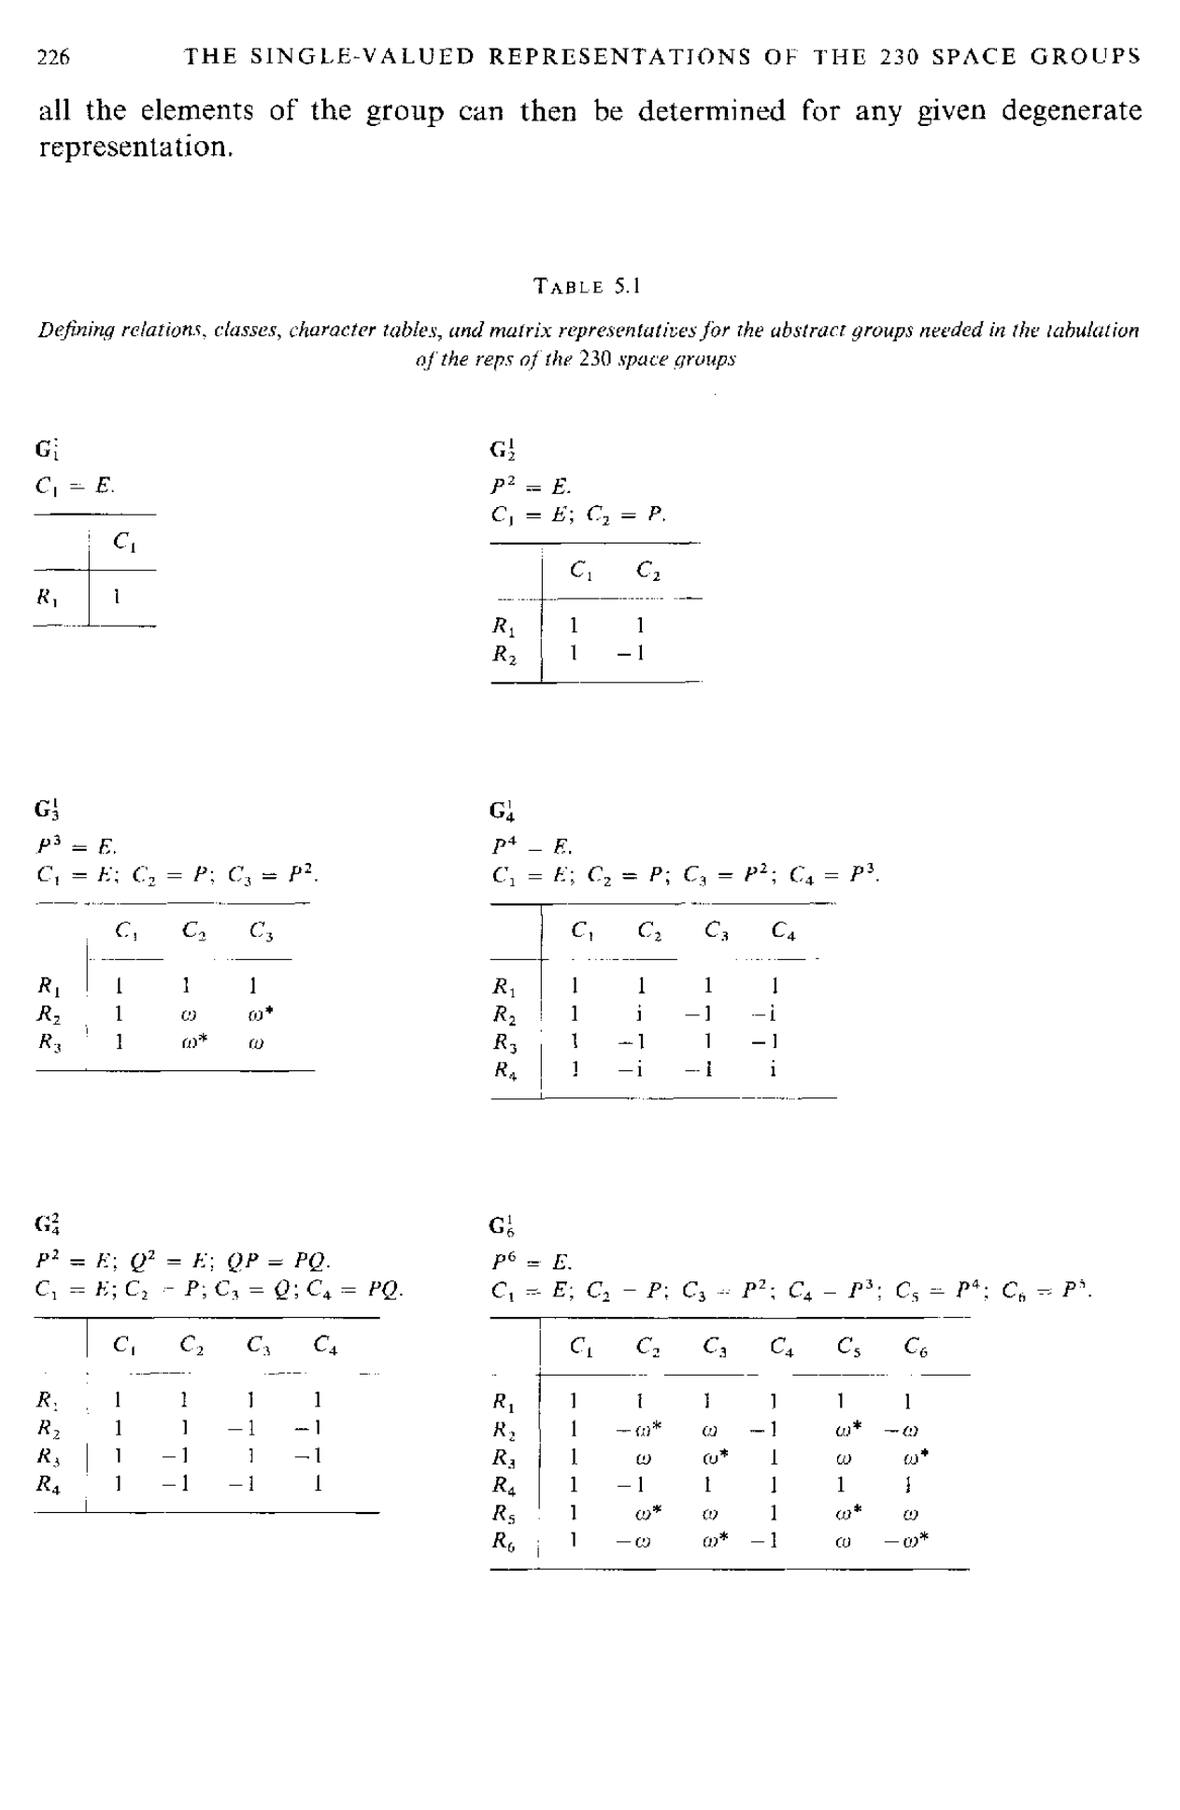
\includegraphics[width=0.86\textwidth]{c5_t51_p01.jpg}
\caption*{\textbf{表 5.1}\ 抽象群的定义关系、类、特征标表与矩阵代表（230 个空间群的表示表所需；原书扫描，第 1 页，共 60 页）}
\end{figure}
\begin{figure}[H]
\centering
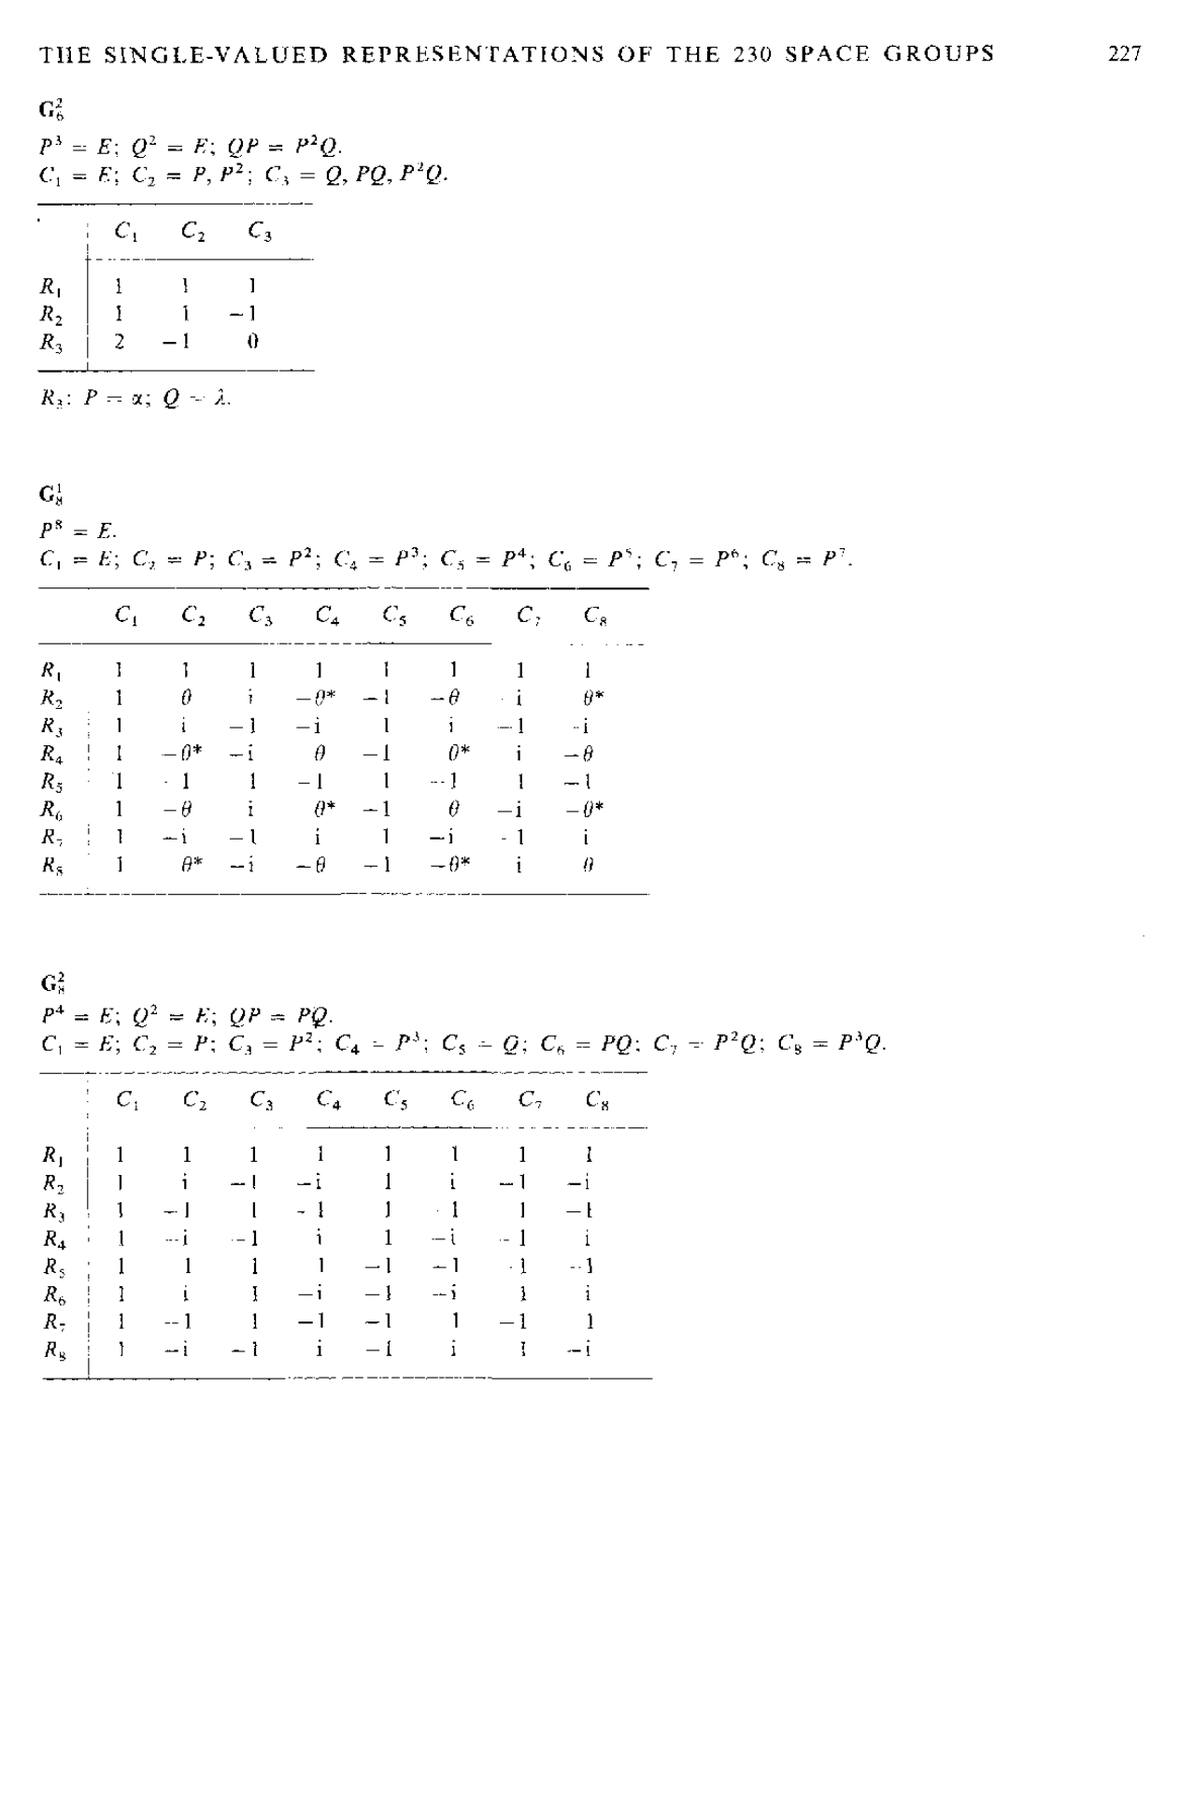
\includegraphics[width=0.86\textwidth]{c5_t51_p02.jpg}
\caption*{\textbf{表 5.1}（第 2 页，共 60 页；原书第 227 页）}
\end{figure}
\begin{figure}[H]
\centering
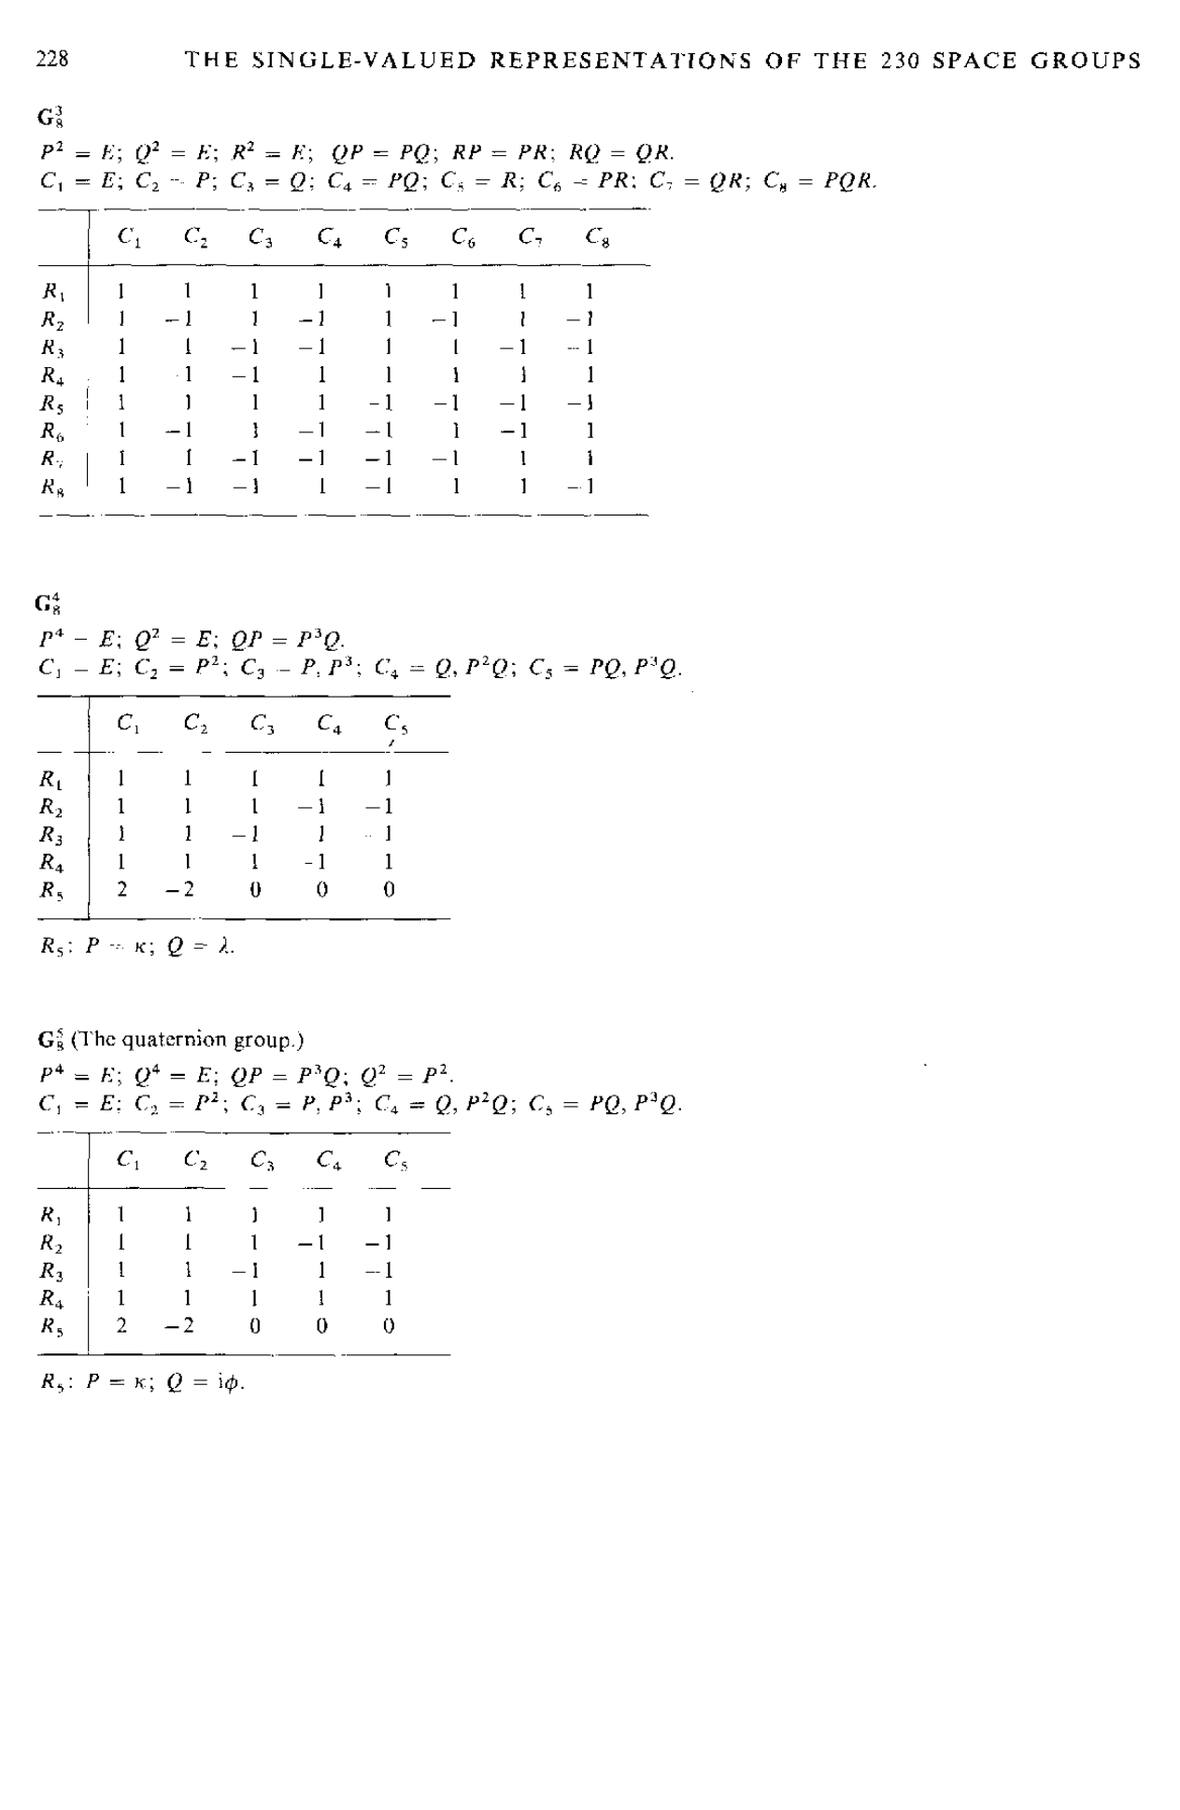
\includegraphics[width=0.86\textwidth]{c5_t51_p03.jpg}
\caption*{\textbf{表 5.1}（第 3 页，共 60 页；原书第 228 页）}
\end{figure}
\begin{figure}[H]
\centering
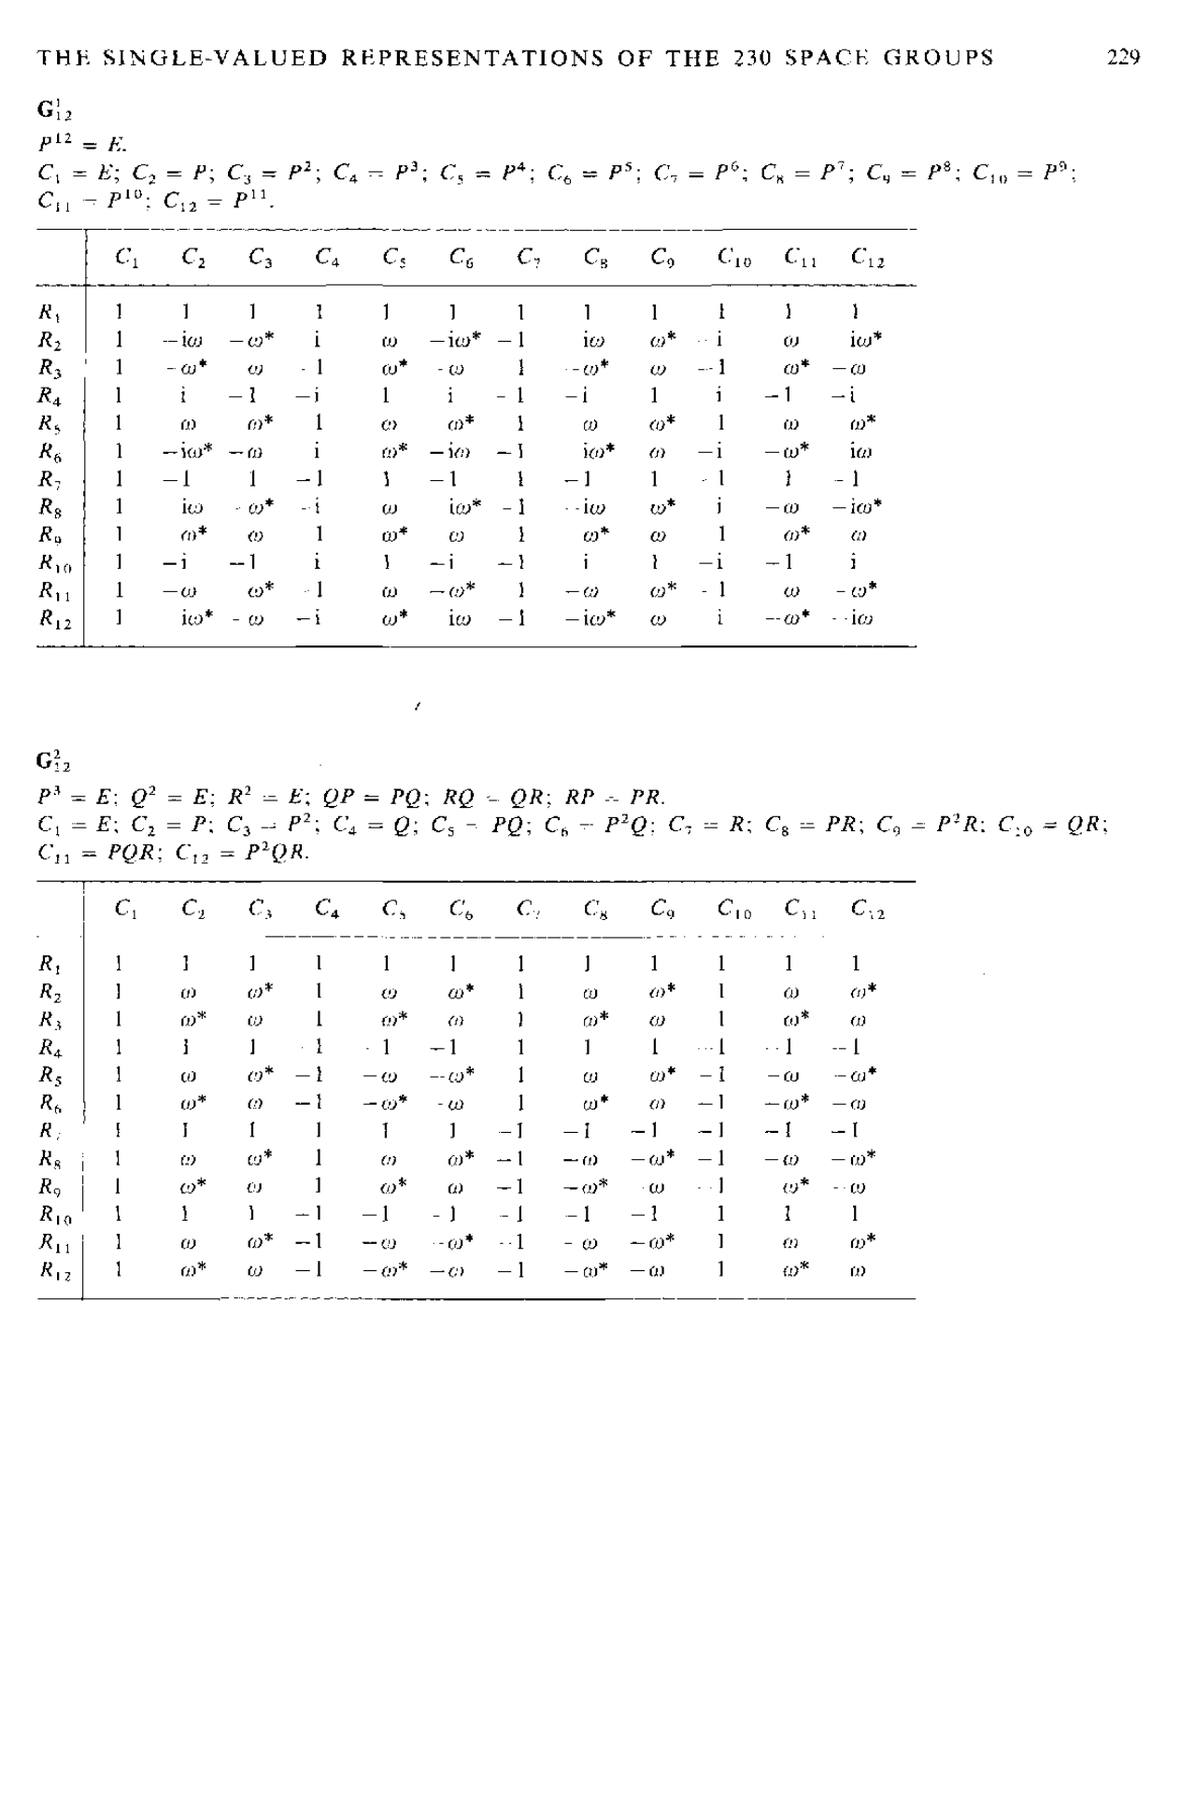
\includegraphics[width=0.86\textwidth]{c5_t51_p04.jpg}
\caption*{\textbf{表 5.1}（第 4 页，共 60 页；原书第 229 页）}
\end{figure}
\begin{figure}[H]
\centering
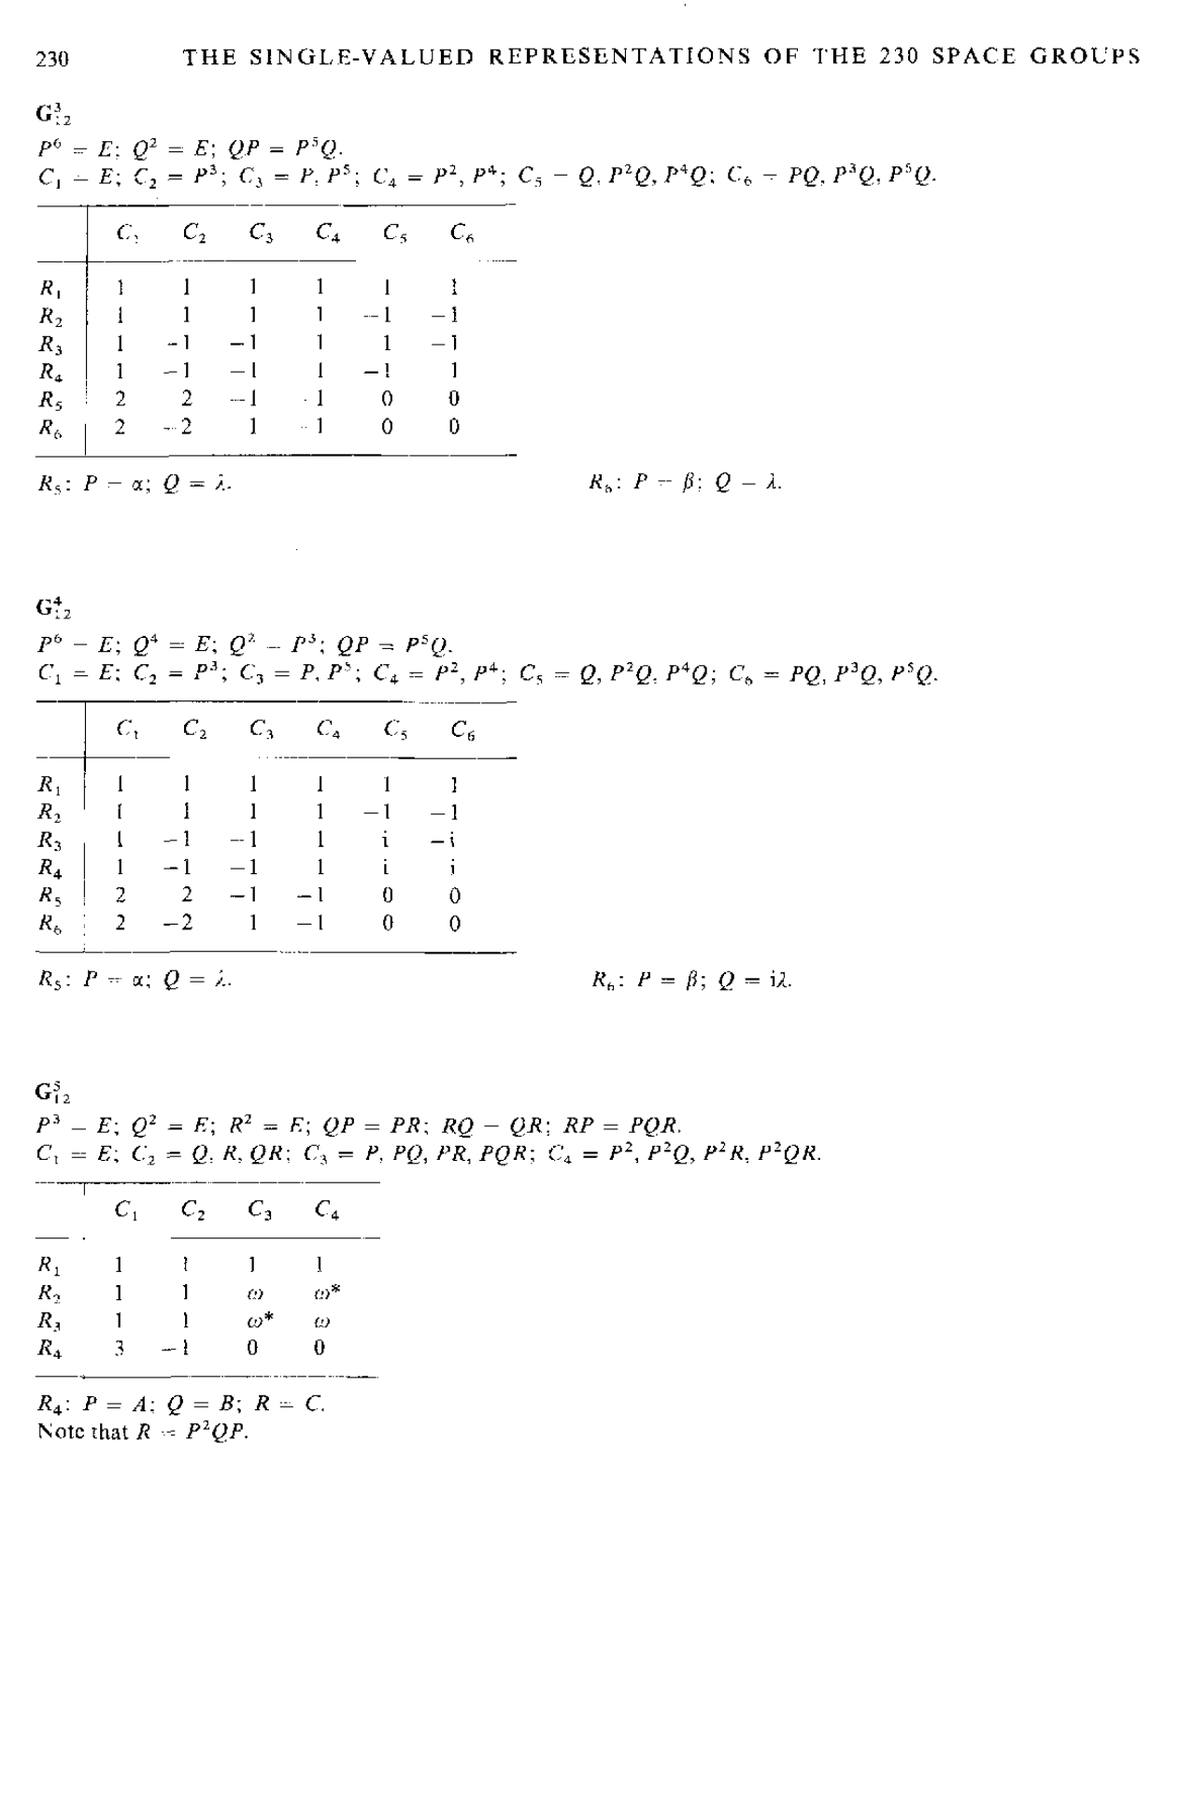
\includegraphics[width=0.86\textwidth]{c5_t51_p05.jpg}
\caption*{\textbf{表 5.1}（第 5 页，共 60 页；原书第 230 页）}
\end{figure}
\begin{figure}[H]
\centering
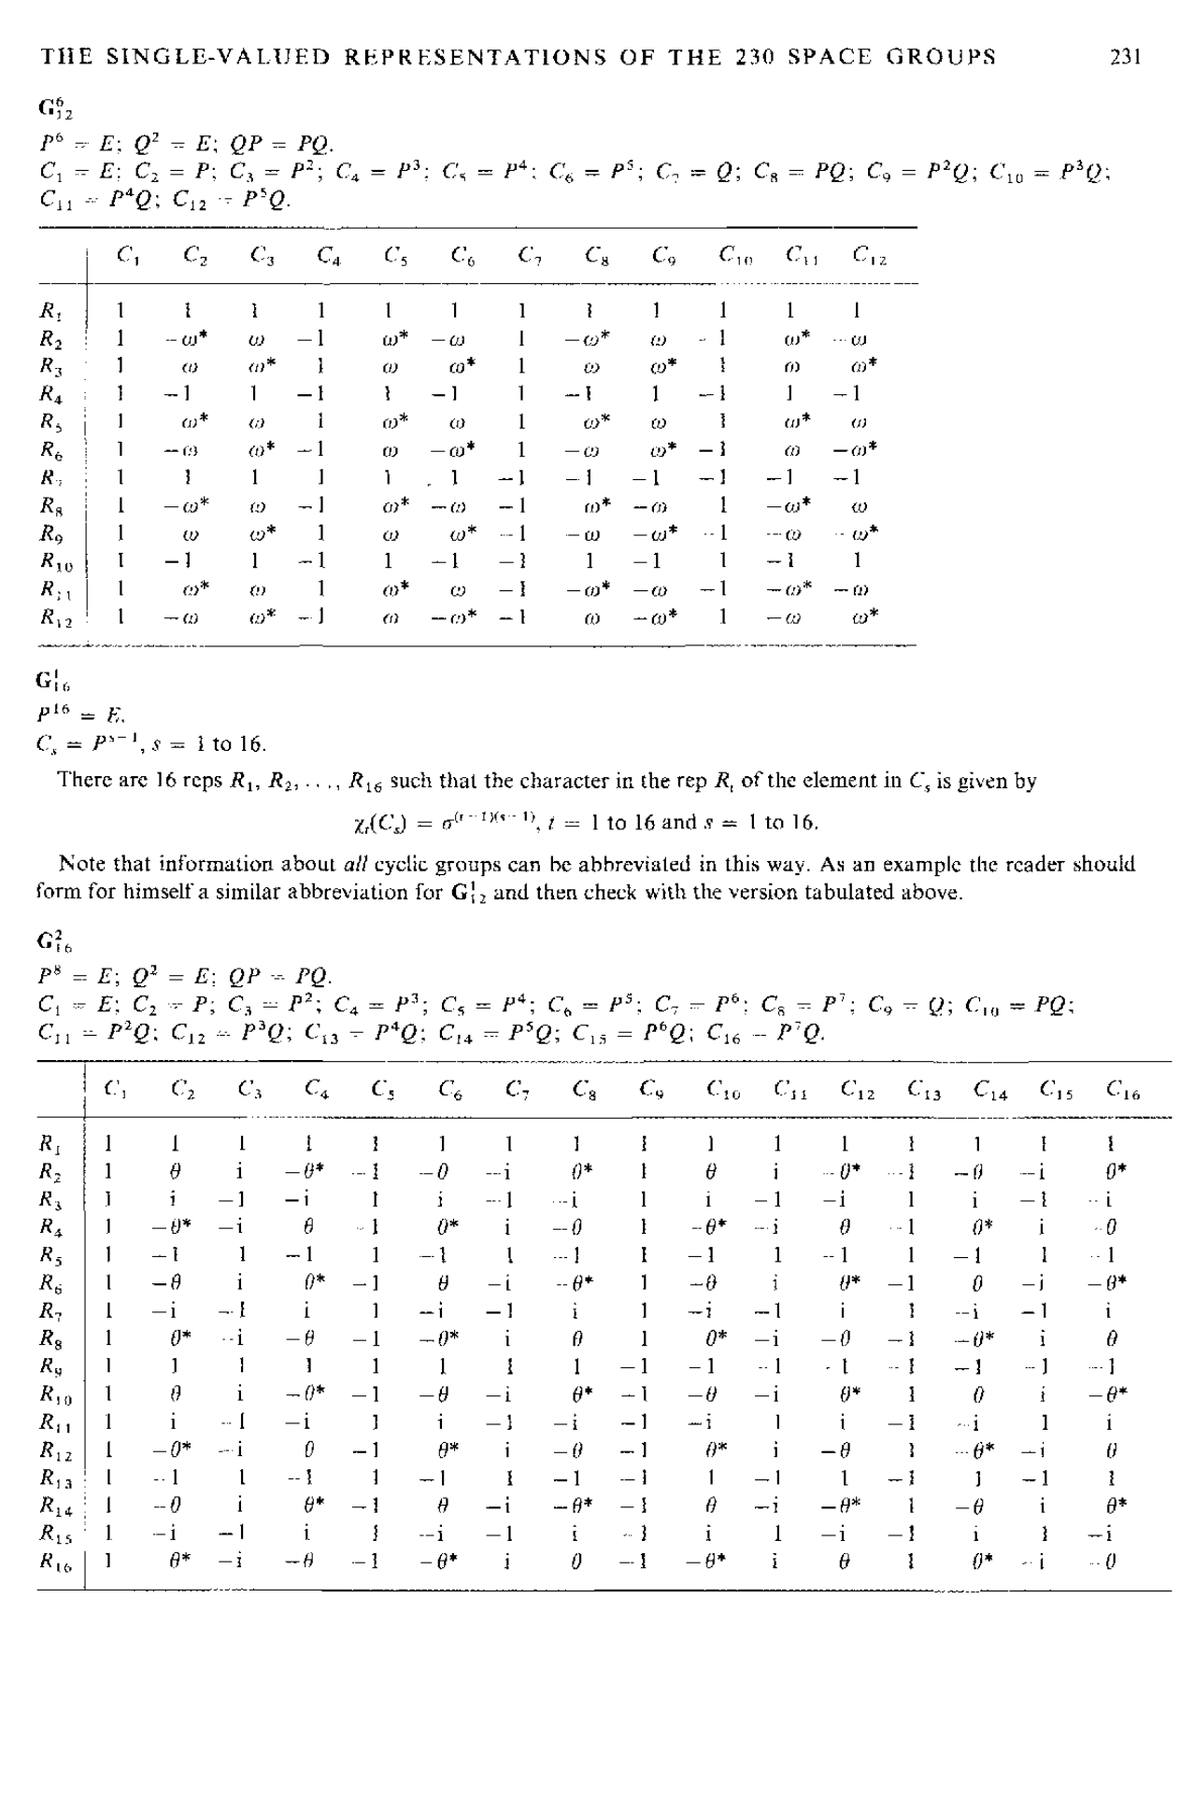
\includegraphics[width=0.86\textwidth]{c5_t51_p06.jpg}
\caption*{\textbf{表 5.1}（第 6 页，共 60 页；原书第 231 页）}
\end{figure}
\begin{figure}[H]
\centering
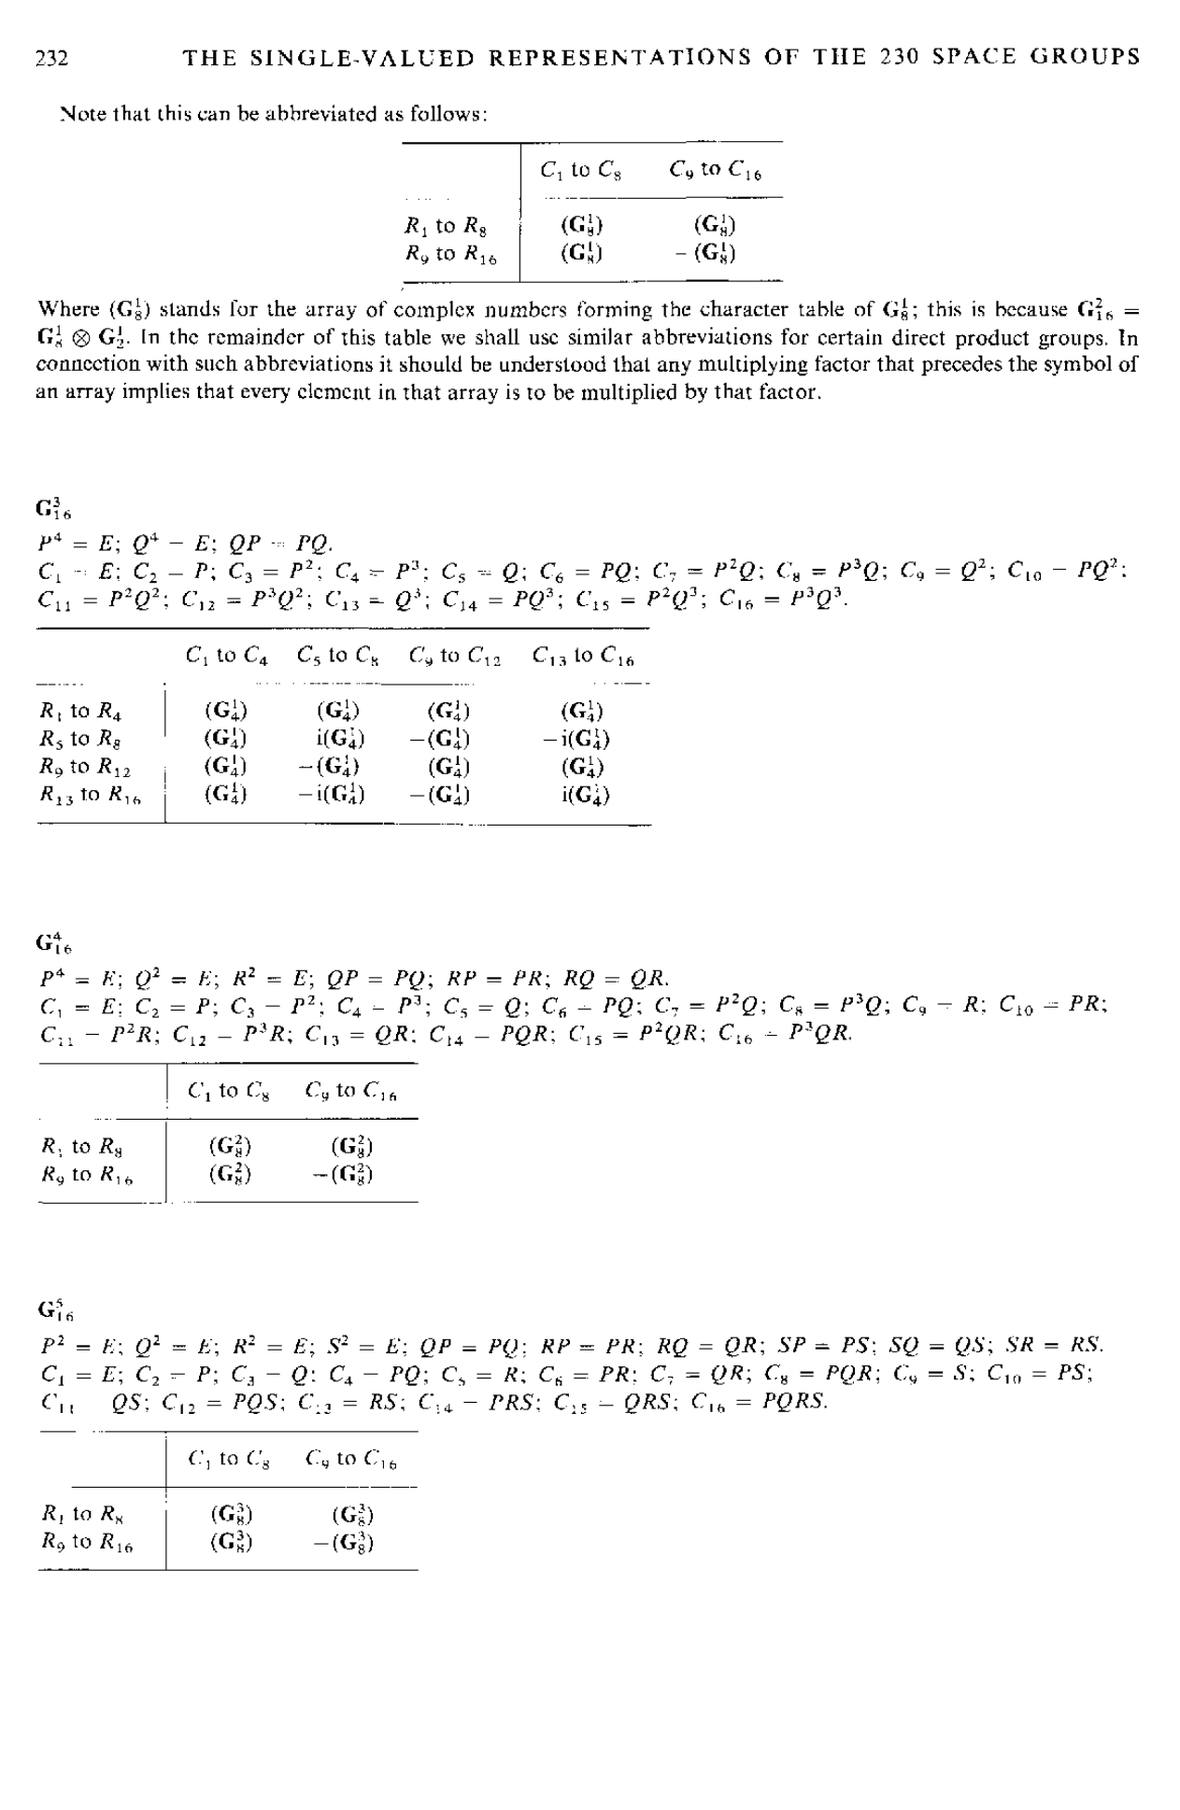
\includegraphics[width=0.86\textwidth]{c5_t51_p07.jpg}
\caption*{\textbf{表 5.1}（第 7 页，共 60 页；原书第 232 页）}
\end{figure}
\begin{figure}[H]
\centering
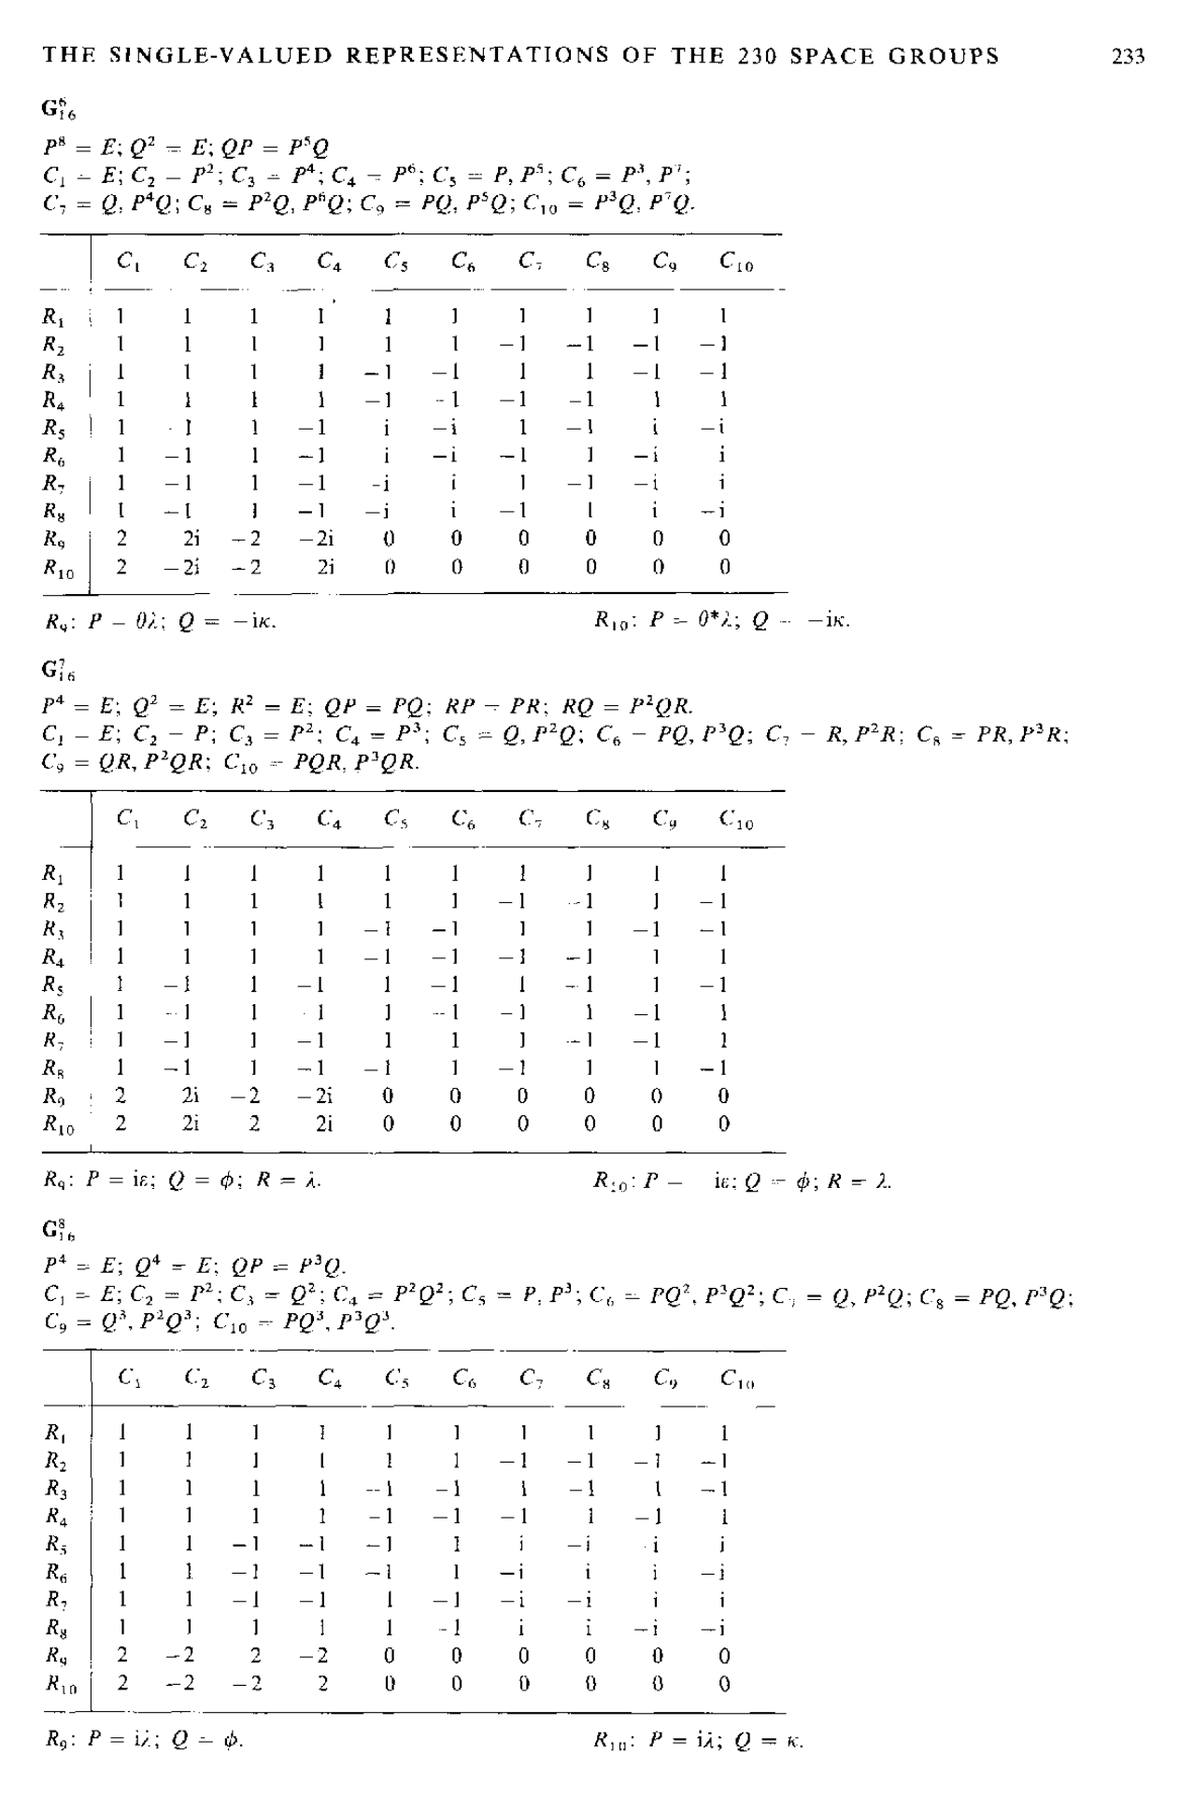
\includegraphics[width=0.86\textwidth]{c5_t51_p08.jpg}
\caption*{\textbf{表 5.1}（第 8 页，共 60 页；原书第 233 页）}
\end{figure}
\begin{figure}[H]
\centering
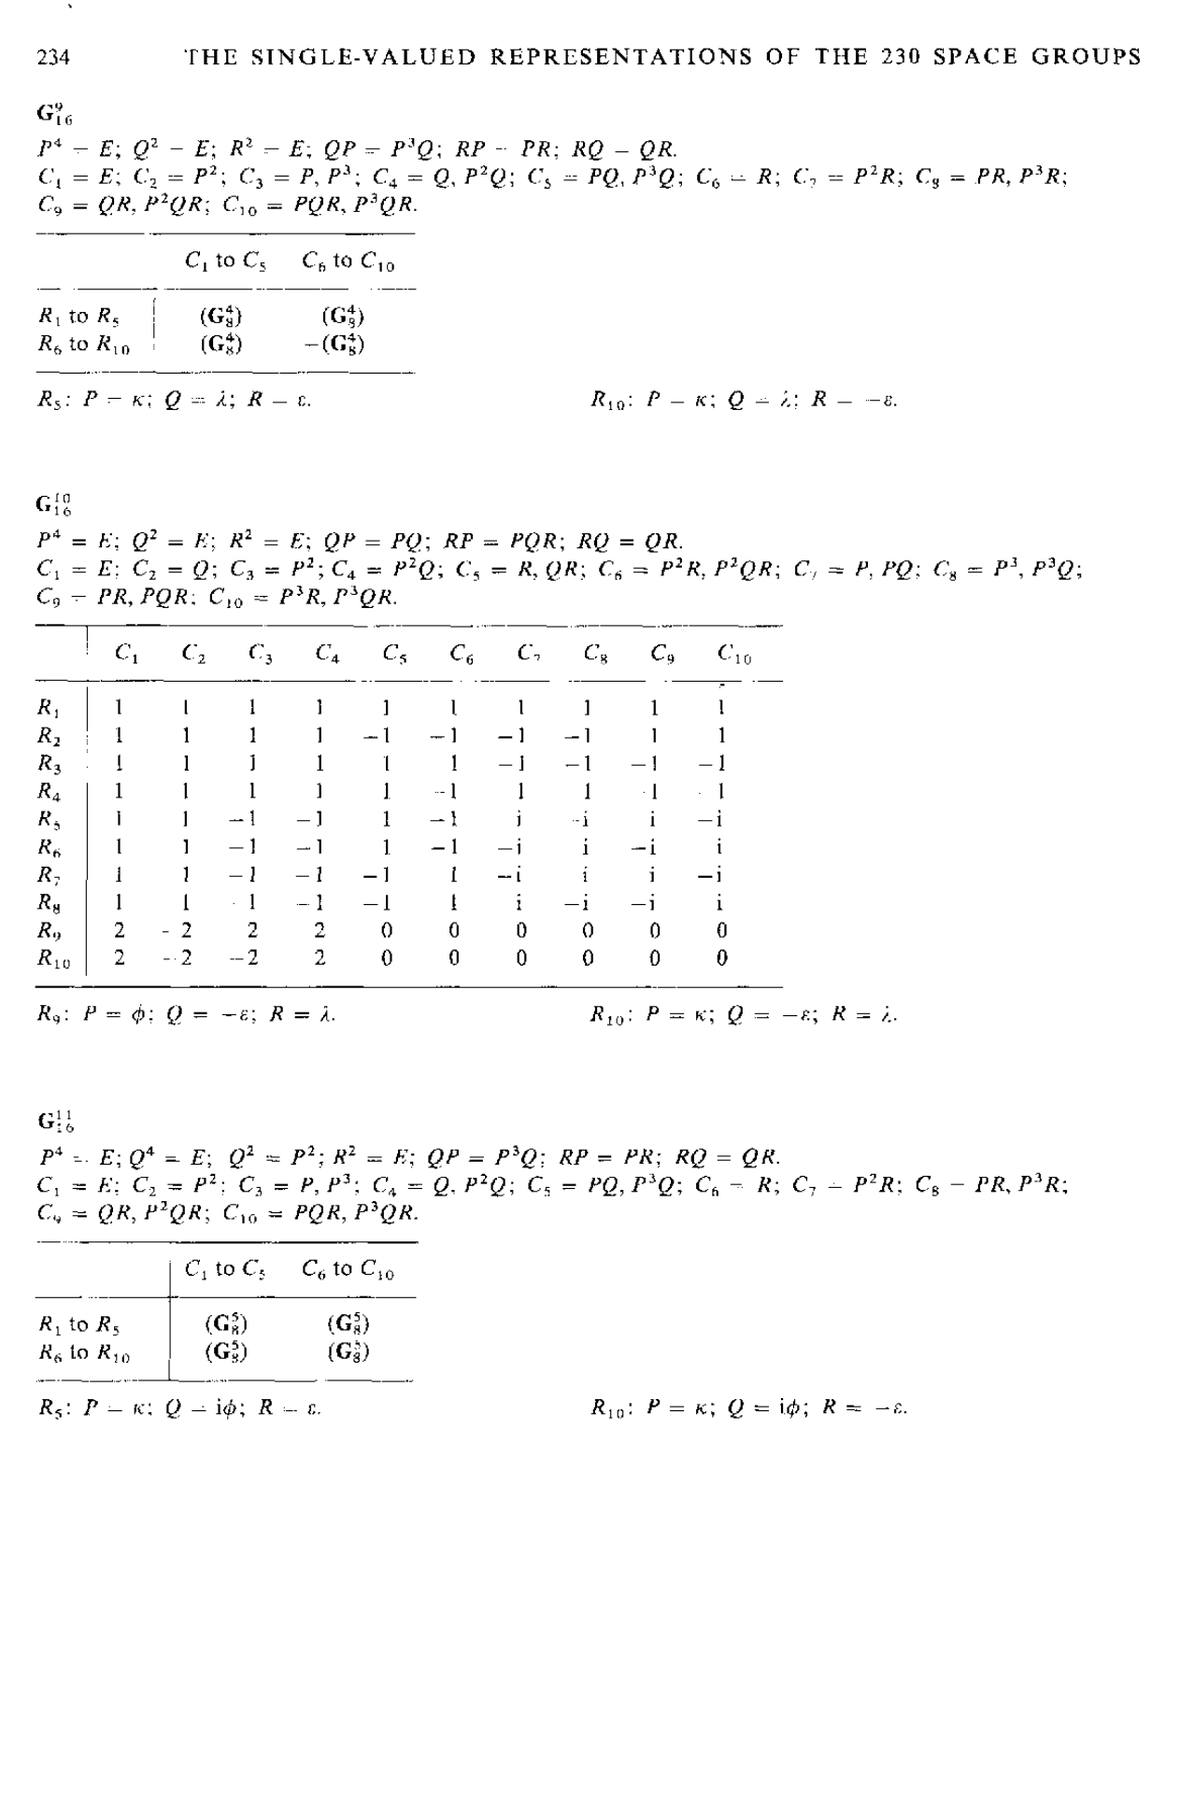
\includegraphics[width=0.86\textwidth]{c5_t51_p09.jpg}
\caption*{\textbf{表 5.1}（第 9 页，共 60 页；原书第 234 页）}
\end{figure}
\begin{figure}[H]
\centering
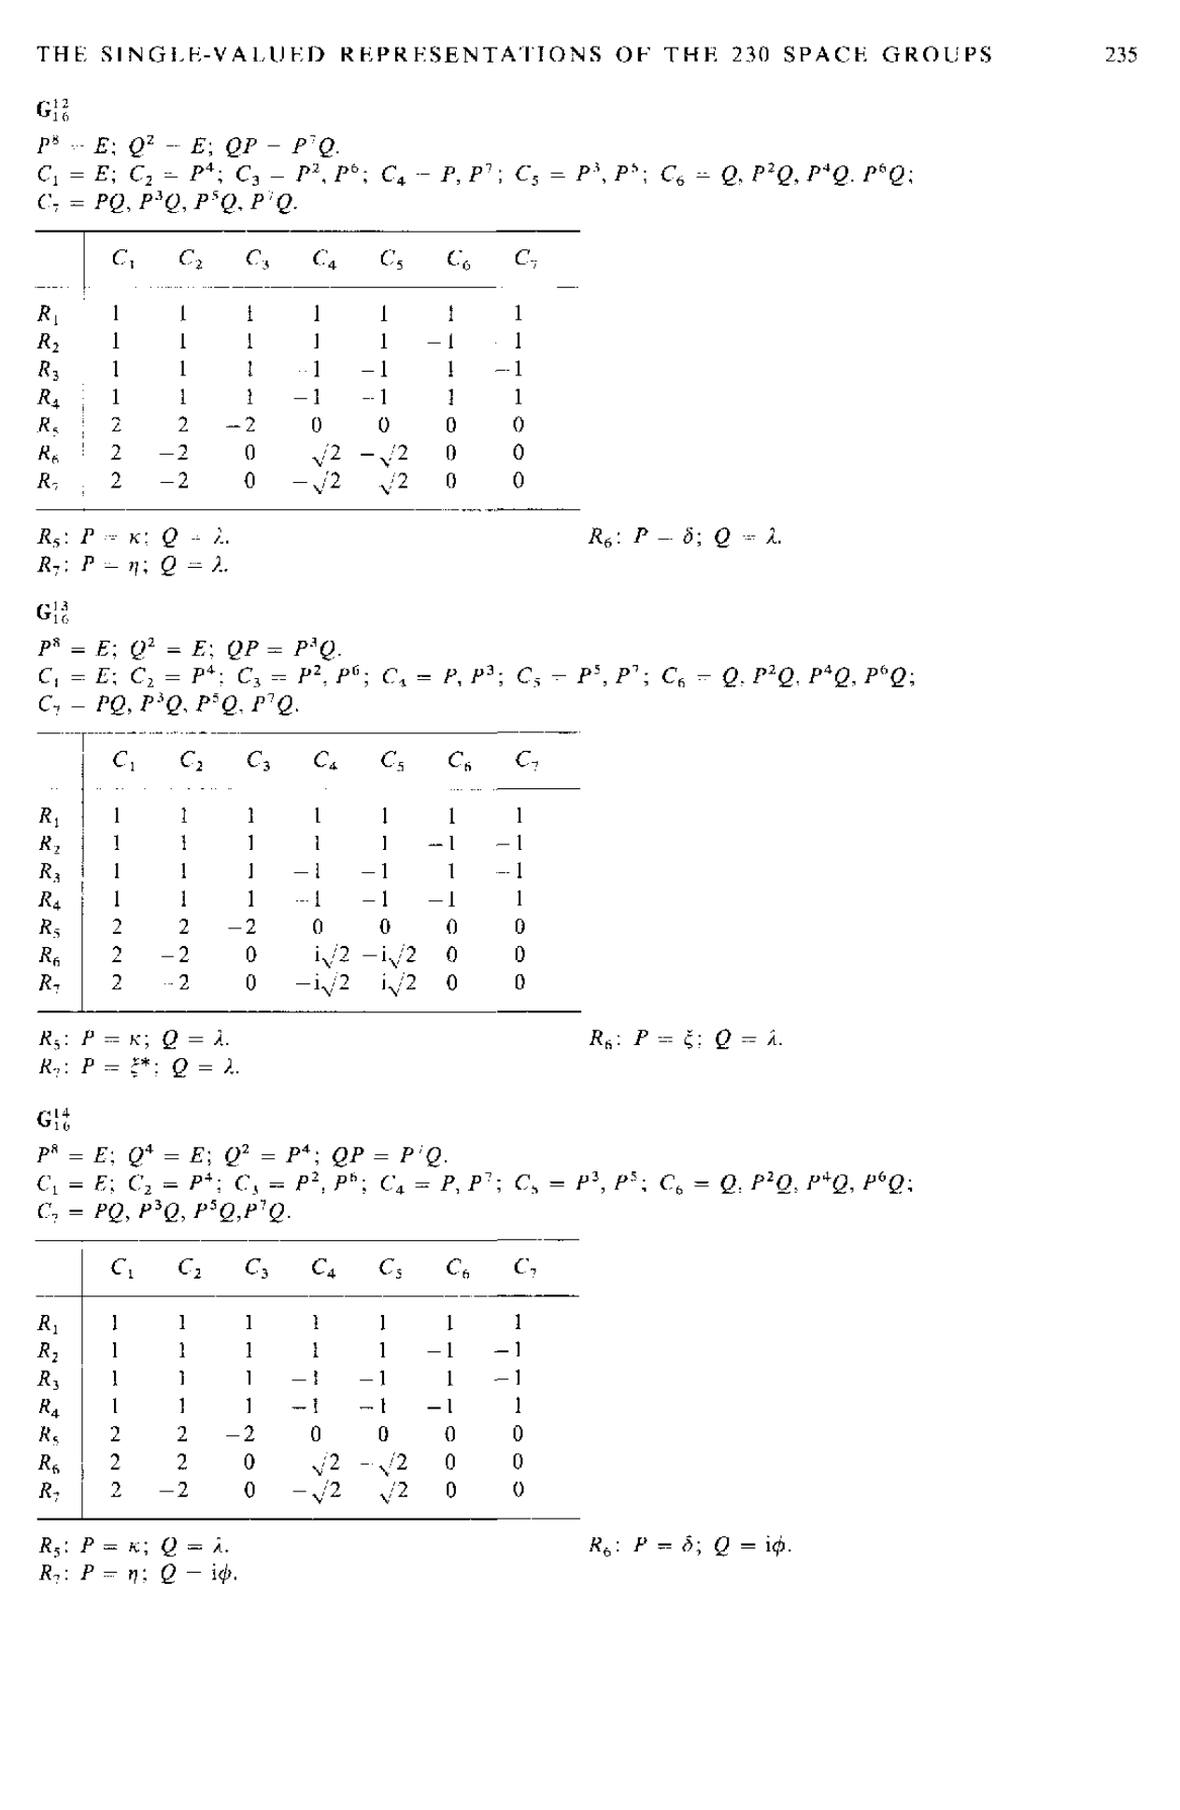
\includegraphics[width=0.86\textwidth]{c5_t51_p10.jpg}
\caption*{\textbf{表 5.1}（第 10 页，共 60 页；原书第 235 页）}
\end{figure}
\begin{figure}[H]
\centering
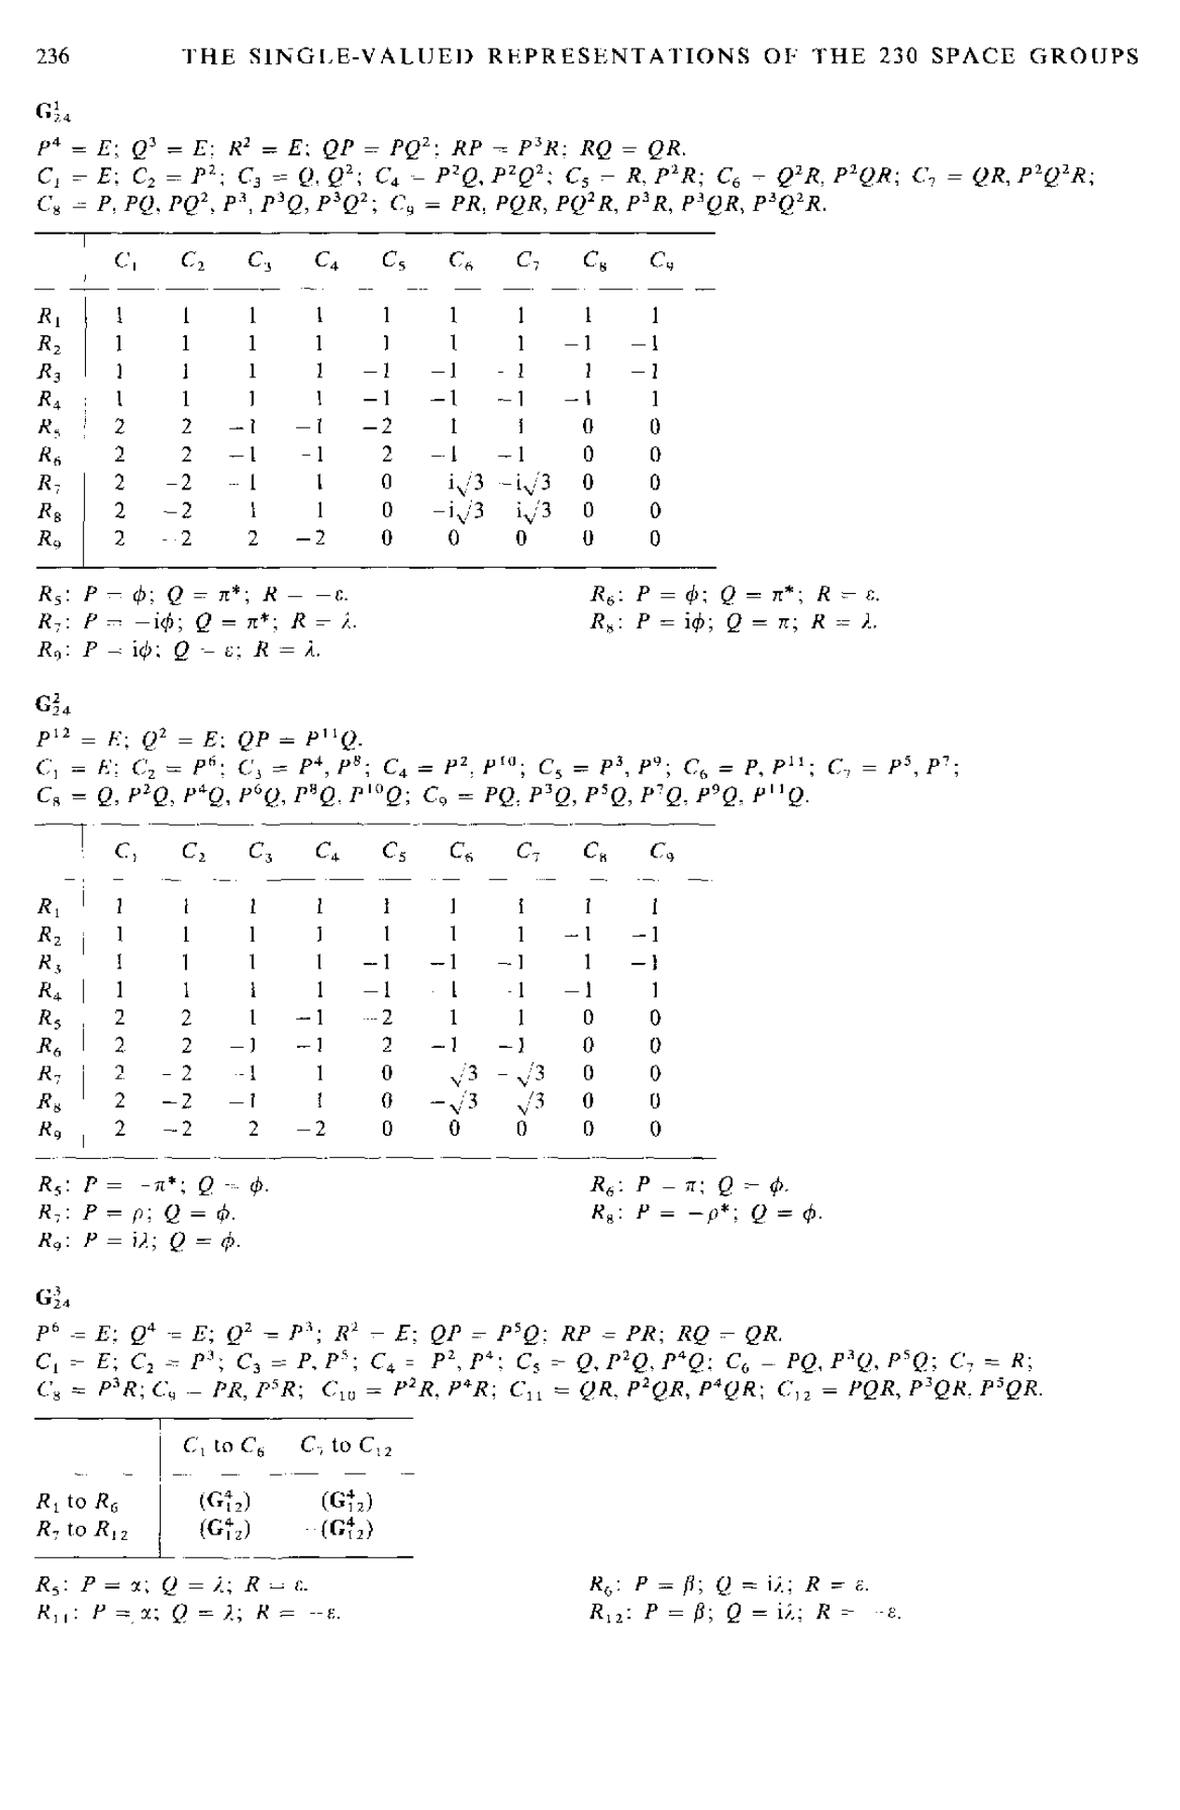
\includegraphics[width=0.86\textwidth]{c5_t51_p11.jpg}
\caption*{\textbf{表 5.1}（第 11 页，共 60 页；原书第 236 页）}
\end{figure}
\begin{figure}[H]
\centering
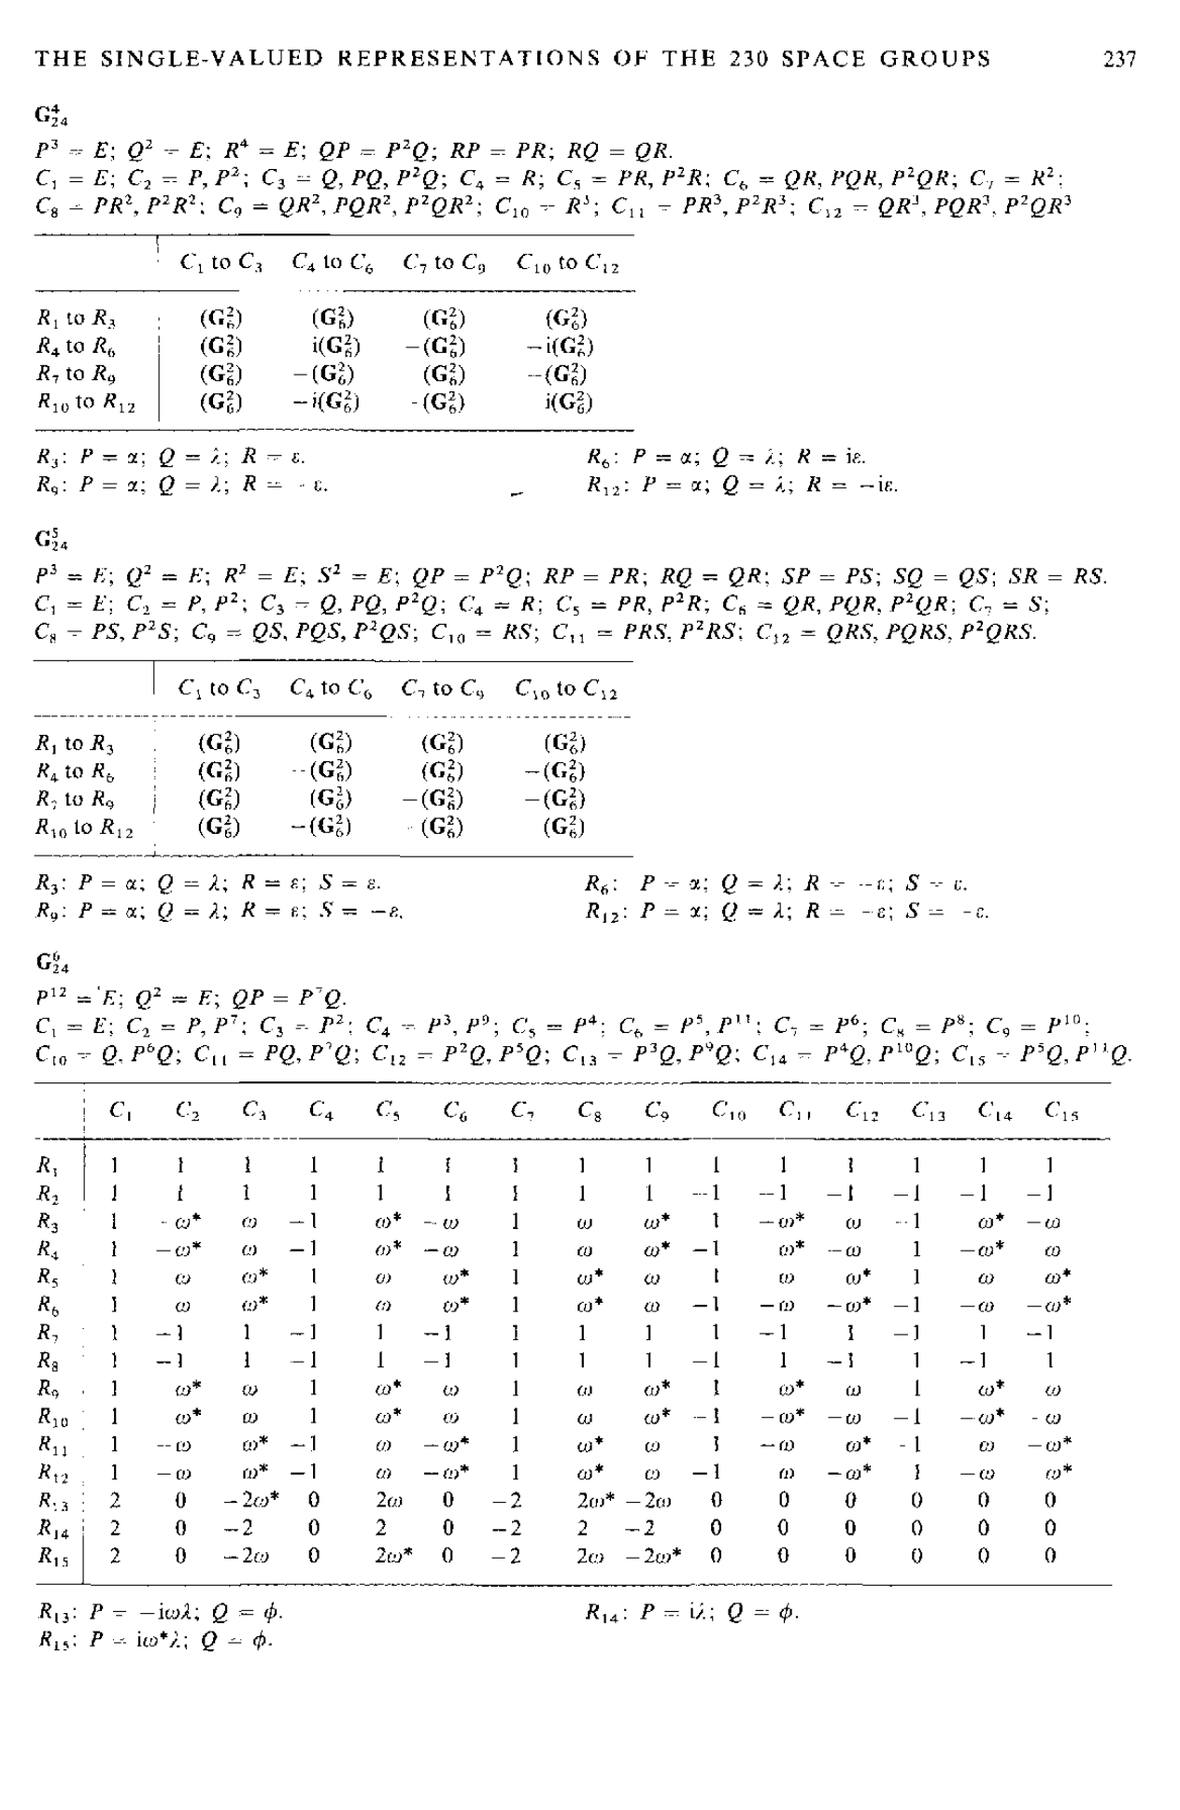
\includegraphics[width=0.86\textwidth]{c5_t51_p12.jpg}
\caption*{\textbf{表 5.1}（第 12 页，共 60 页；原书第 237 页）}
\end{figure}
\begin{figure}[H]
\centering
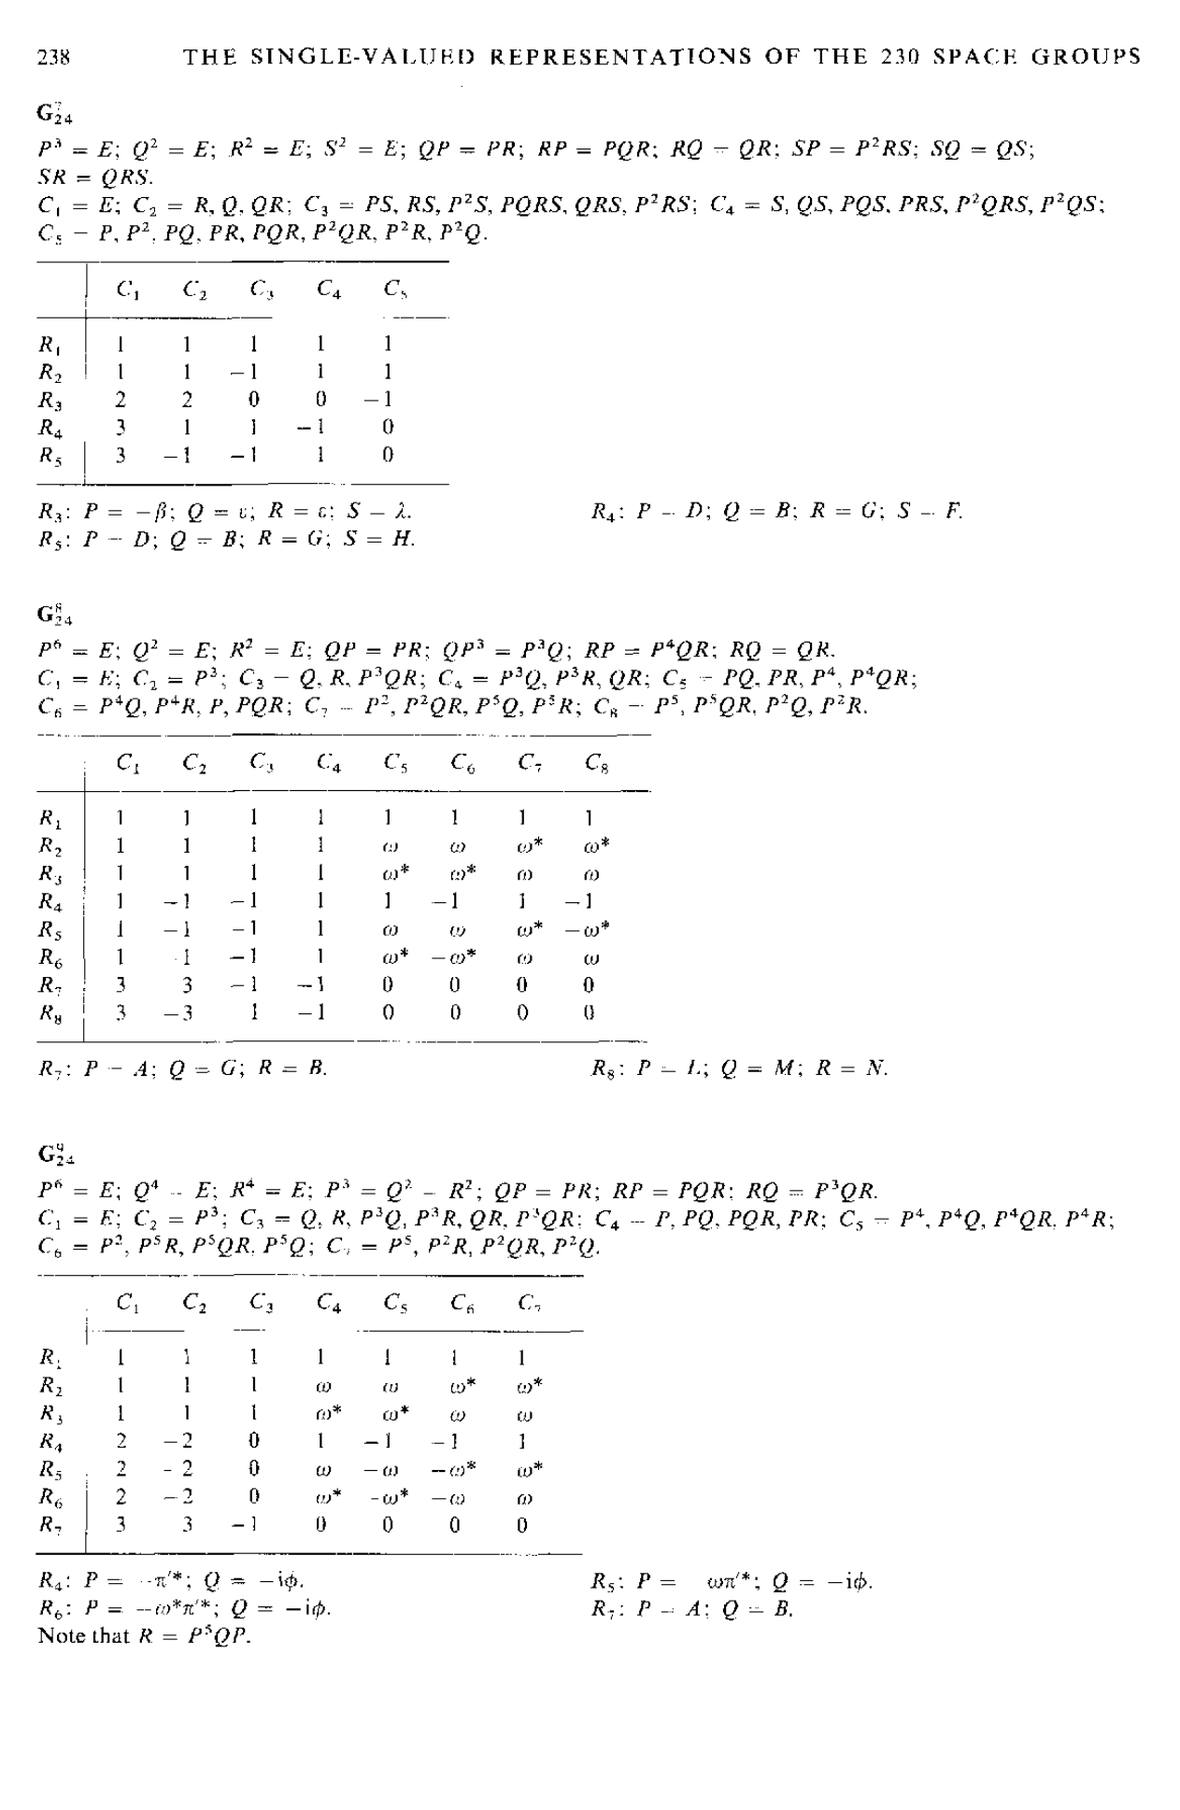
\includegraphics[width=0.86\textwidth]{c5_t51_p13.jpg}
\caption*{\textbf{表 5.1}（第 13 页，共 60 页；原书第 238 页）}
\end{figure}
\begin{figure}[H]
\centering
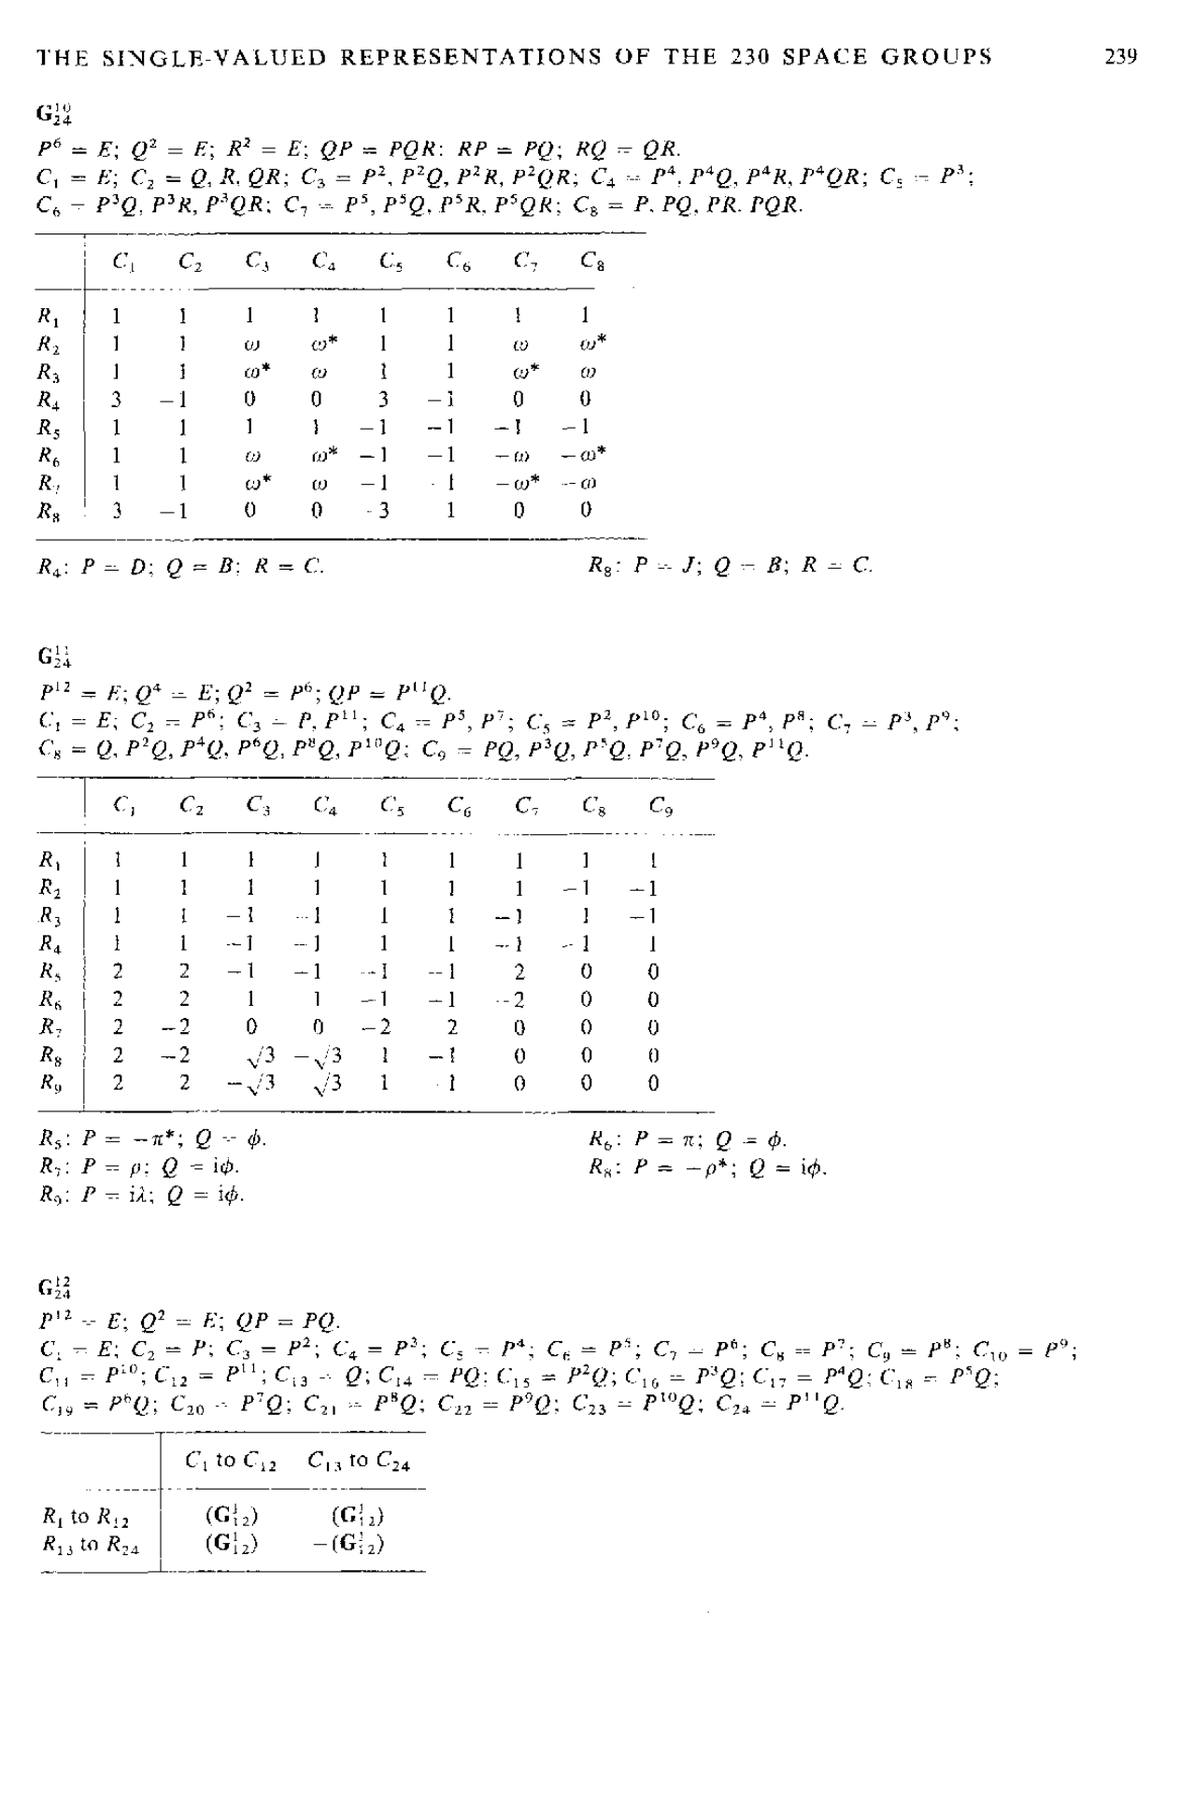
\includegraphics[width=0.86\textwidth]{c5_t51_p14.jpg}
\caption*{\textbf{表 5.1}（第 14 页，共 60 页；原书第 239 页）}
\end{figure}
\begin{figure}[H]
\centering
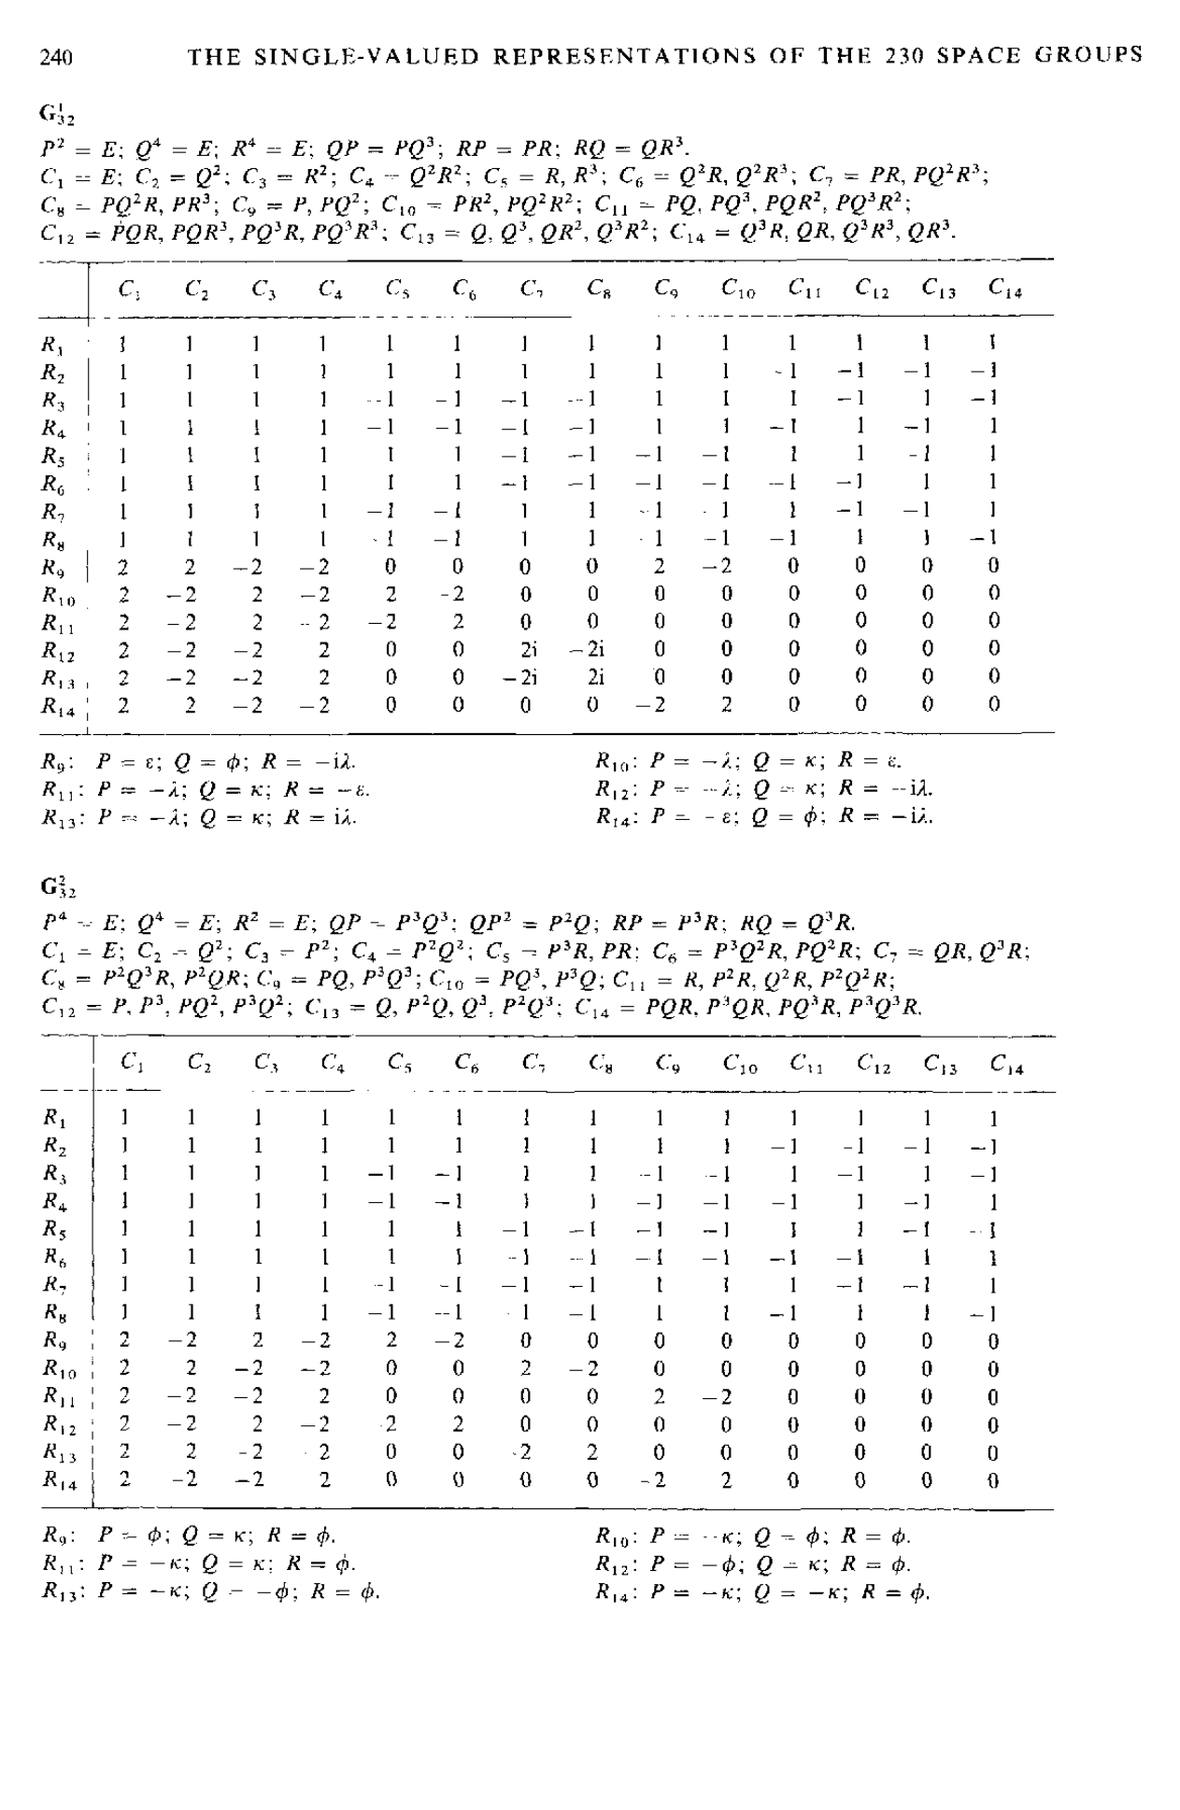
\includegraphics[width=0.86\textwidth]{c5_t51_p15.jpg}
\caption*{\textbf{表 5.1}（第 15 页，共 60 页；原书第 240 页）}
\end{figure}
\begin{figure}[H]
\centering
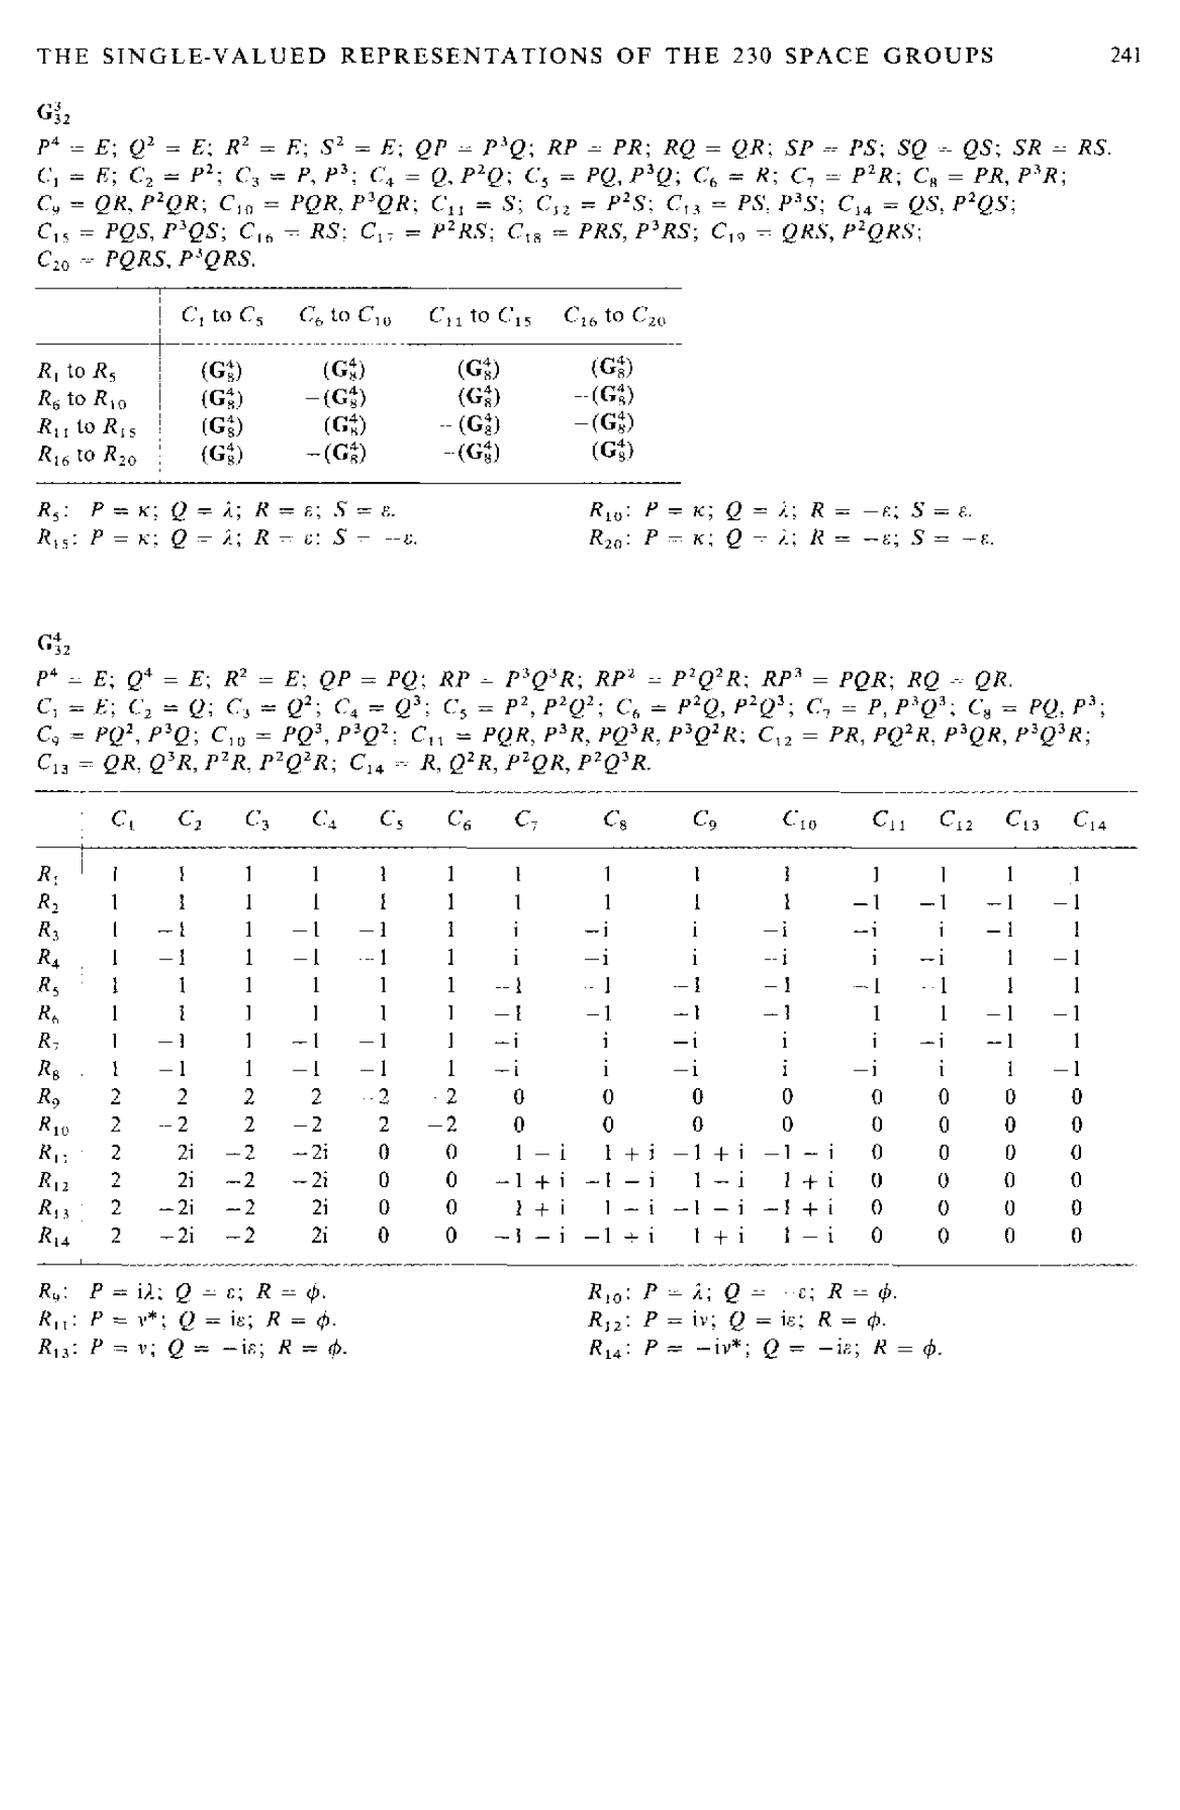
\includegraphics[width=0.86\textwidth]{c5_t51_p16.jpg}
\caption*{\textbf{表 5.1}（第 16 页，共 60 页；原书第 241 页）}
\end{figure}
\begin{figure}[H]
\centering
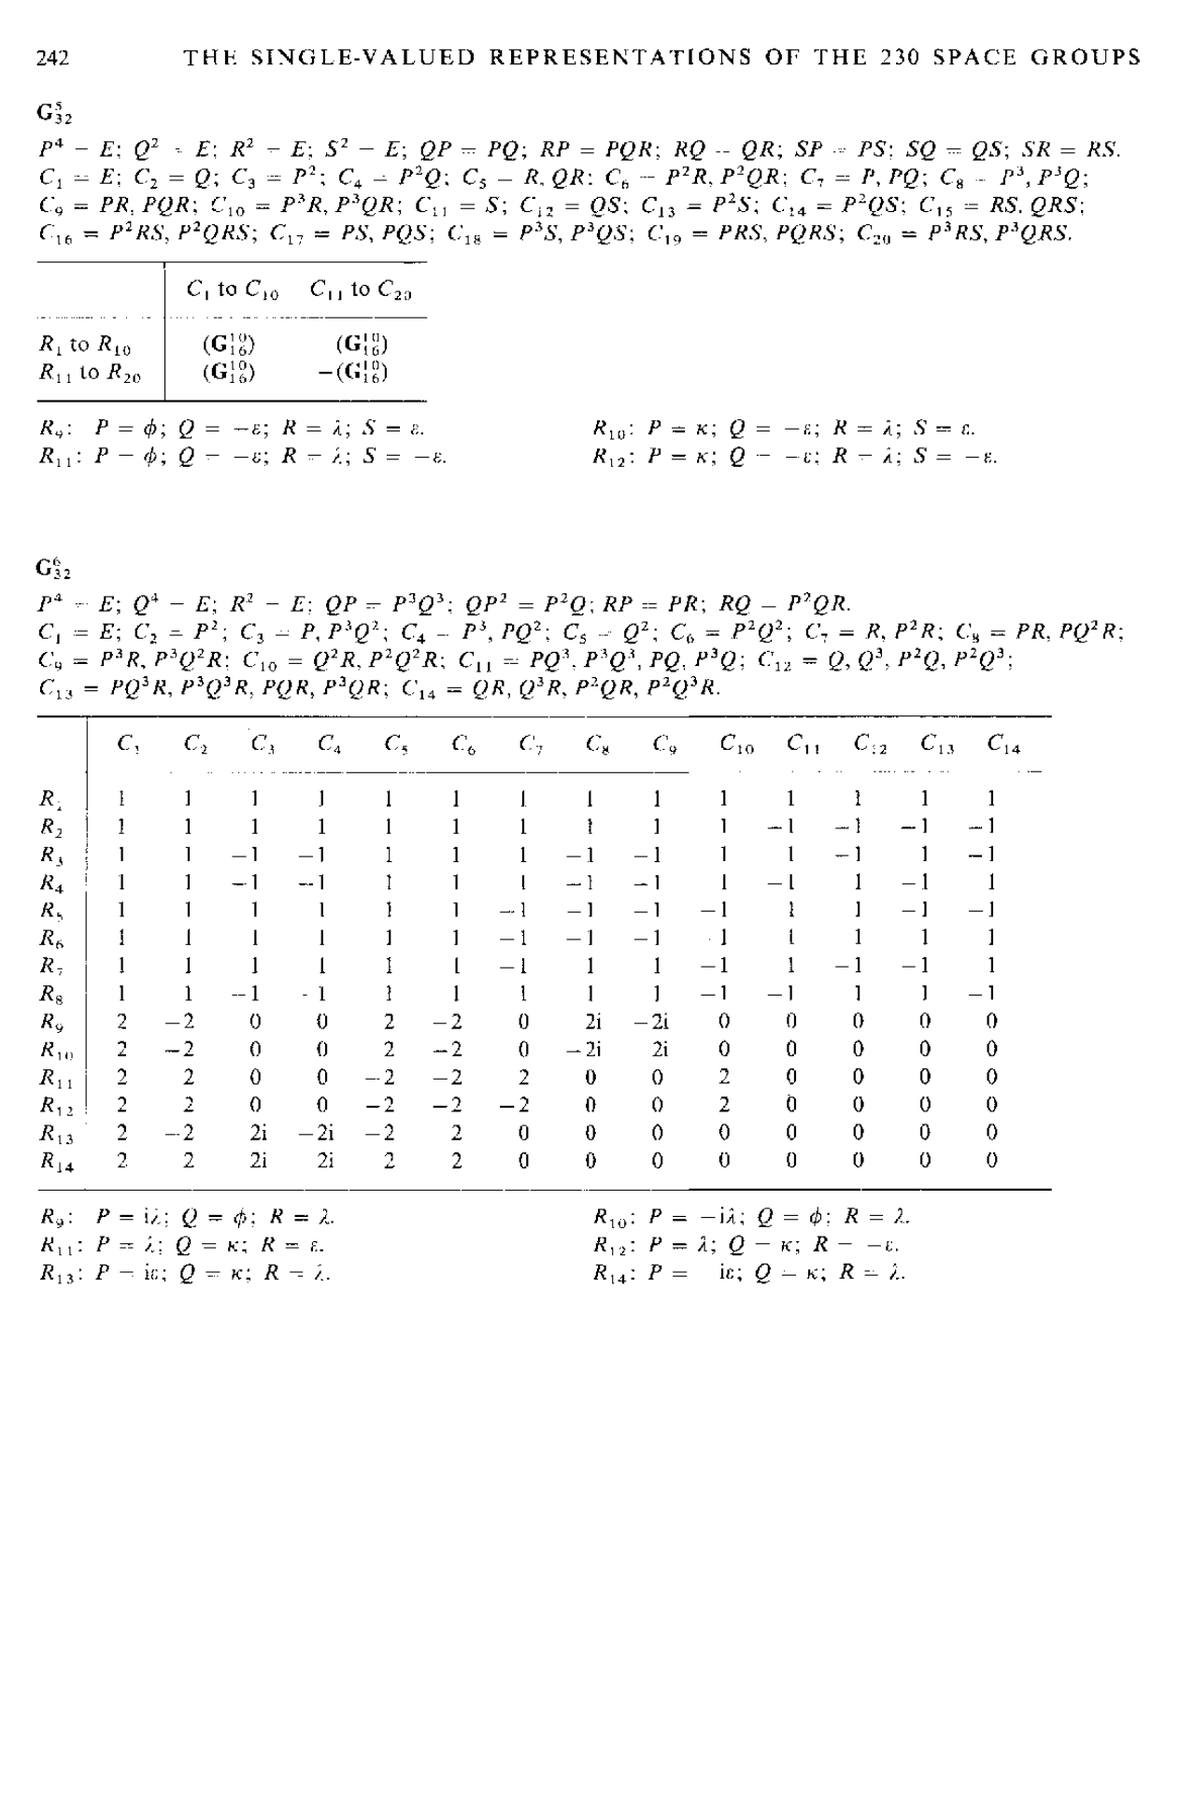
\includegraphics[width=0.86\textwidth]{c5_t51_p17.jpg}
\caption*{\textbf{表 5.1}（第 17 页，共 60 页；原书第 242 页）}
\end{figure}
\begin{figure}[H]
\centering
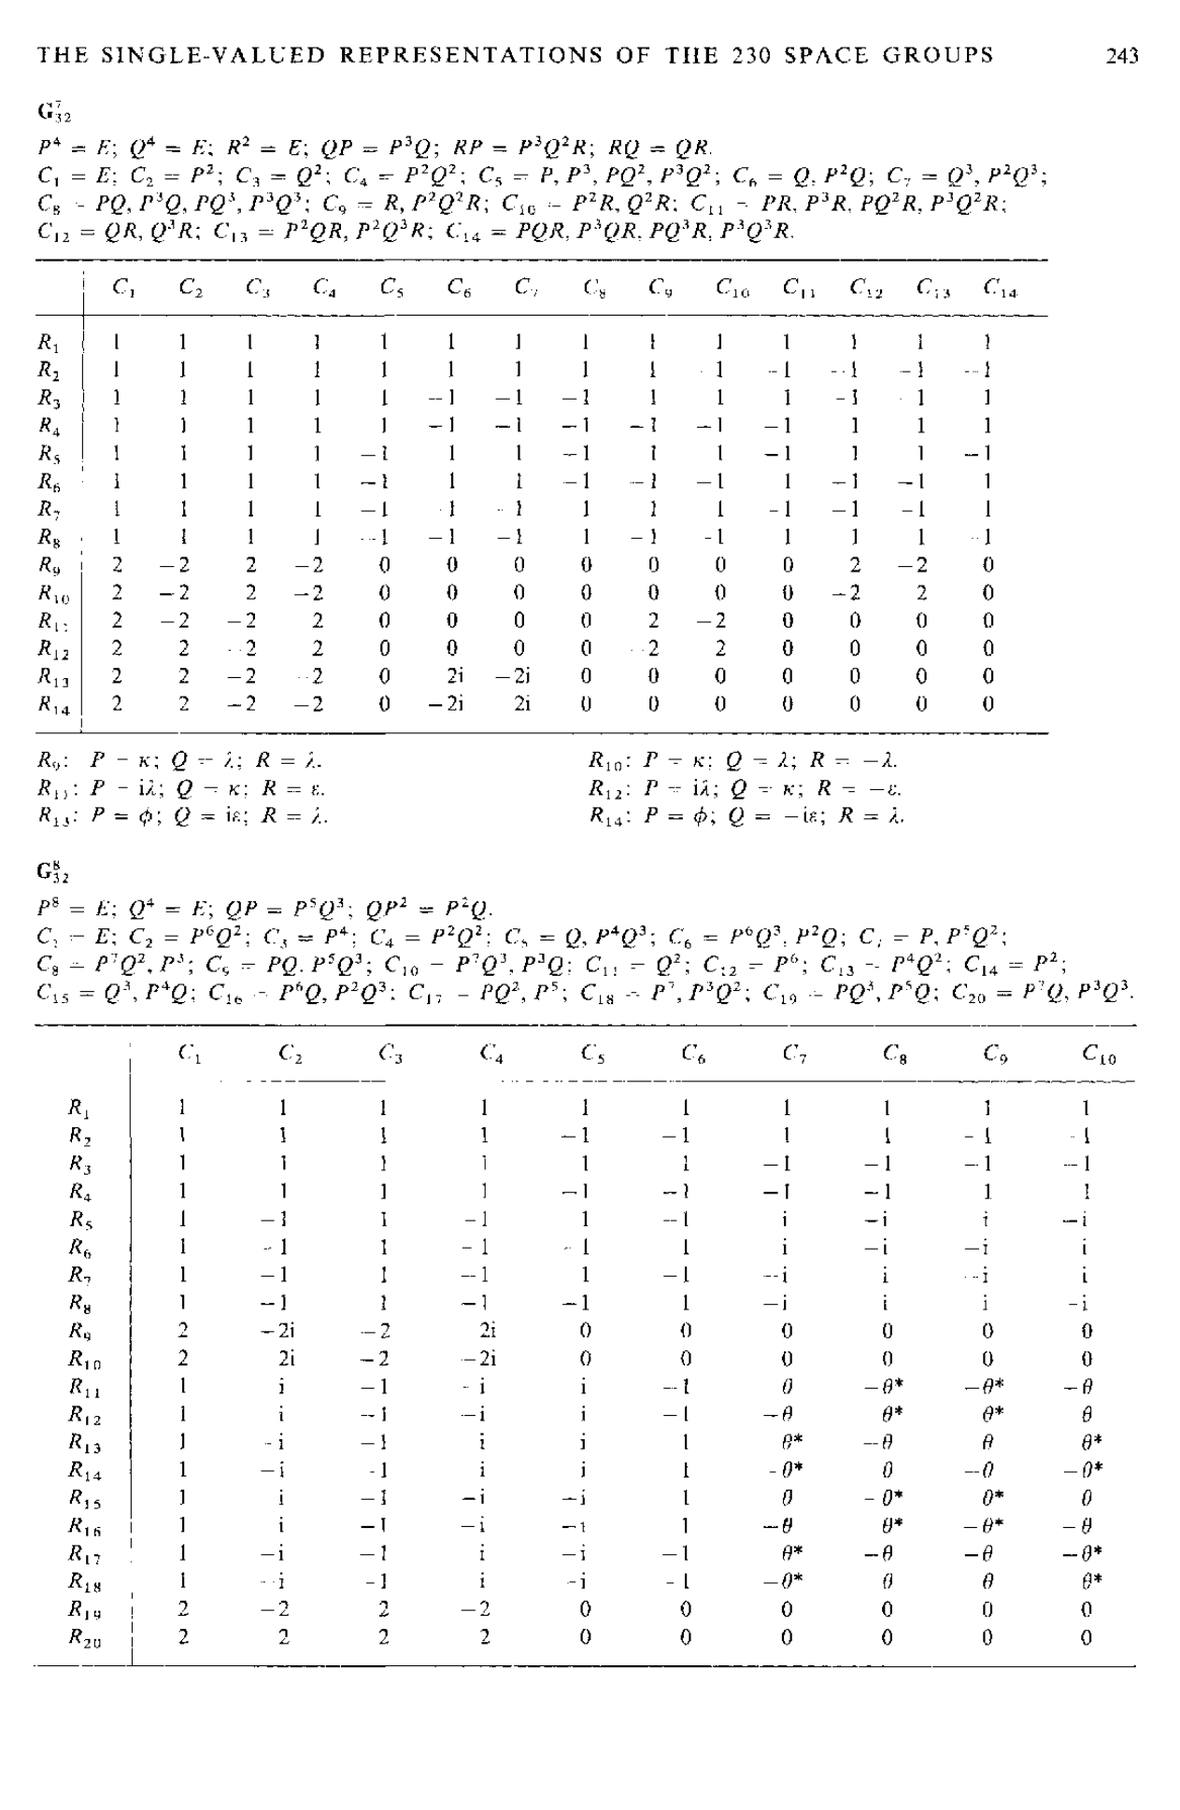
\includegraphics[width=0.86\textwidth]{c5_t51_p18.jpg}
\caption*{\textbf{表 5.1}（第 18 页，共 60 页；原书第 243 页）}
\end{figure}
\begin{figure}[H]
\centering
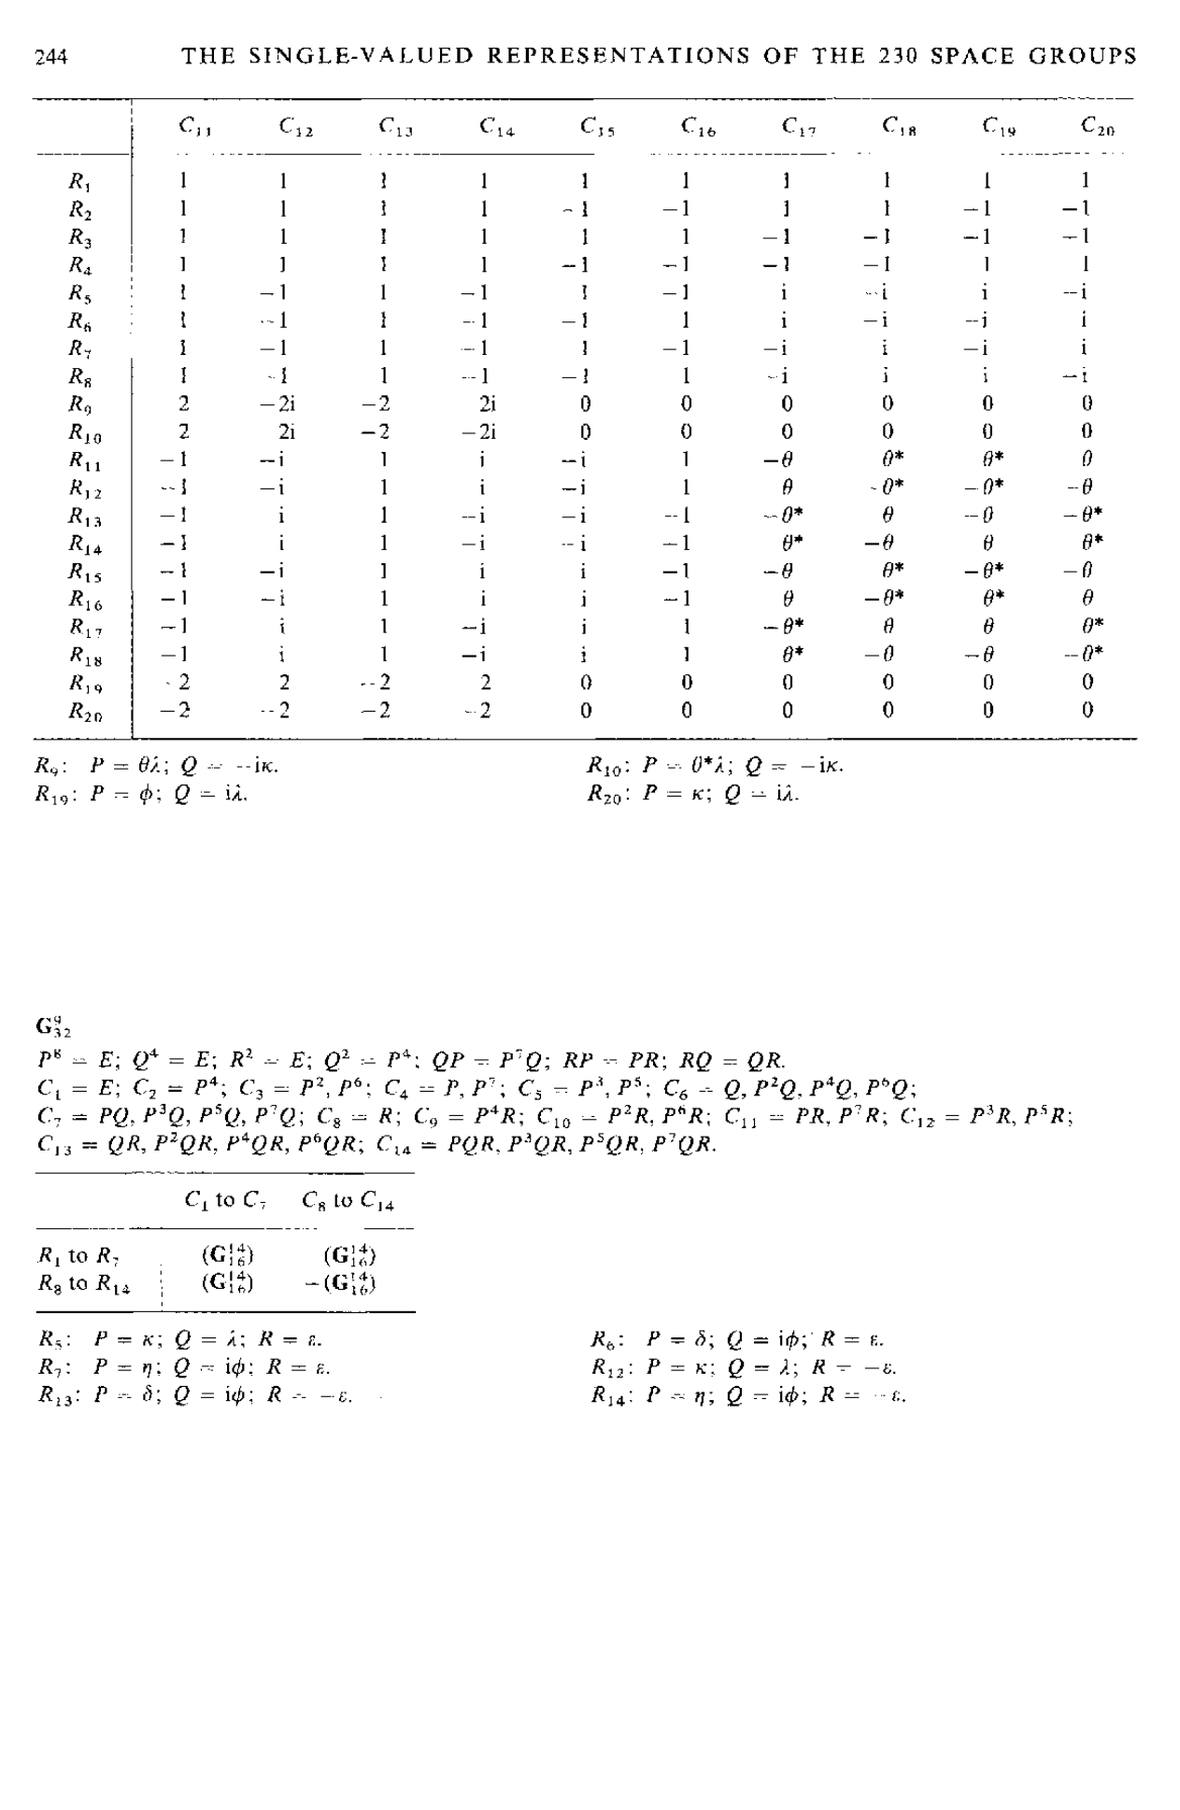
\includegraphics[width=0.86\textwidth]{c5_t51_p19.jpg}
\caption*{\textbf{表 5.1}（第 19 页，共 60 页；原书第 244 页）}
\end{figure}
\begin{figure}[H]
\centering
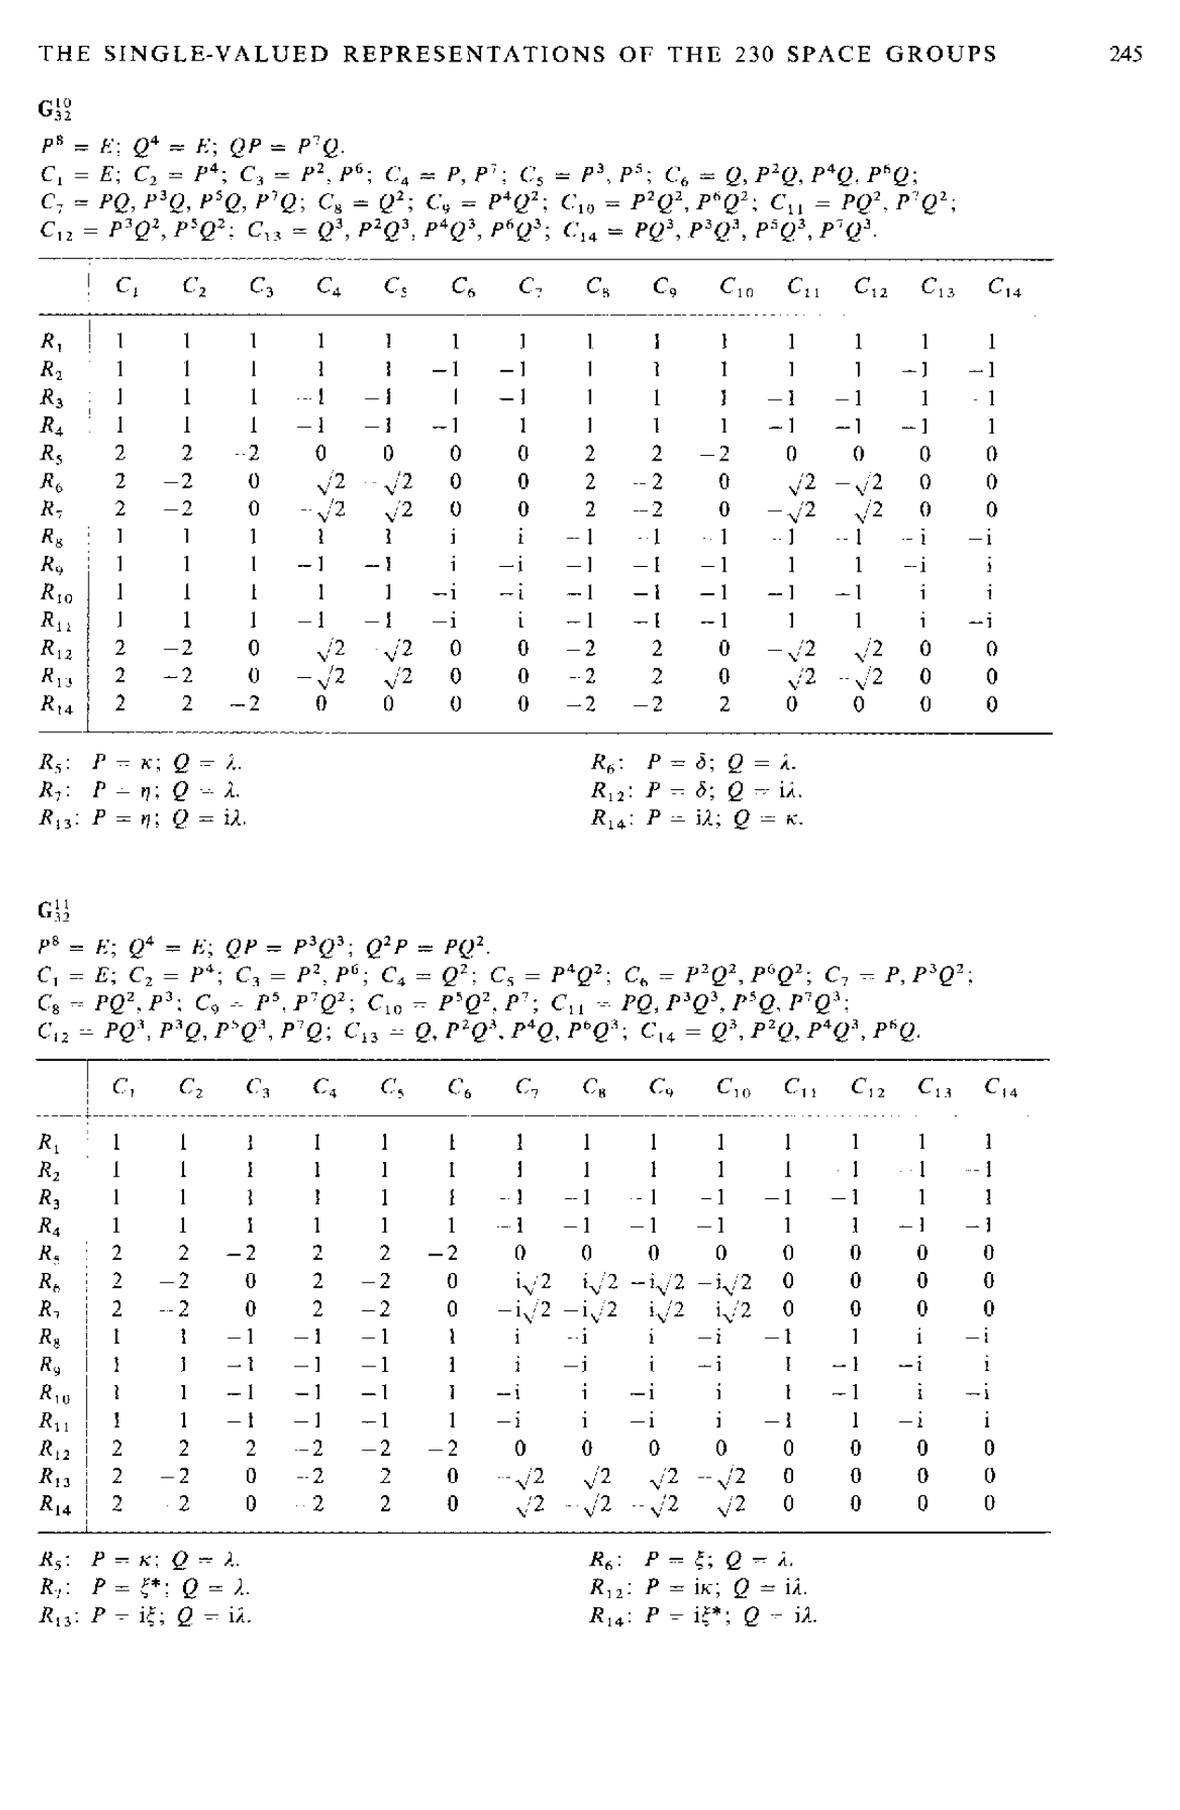
\includegraphics[width=0.86\textwidth]{c5_t51_p20.jpg}
\caption*{\textbf{表 5.1}（第 20 页，共 60 页；原书第 245 页）}
\end{figure}
\begin{figure}[H]
\centering
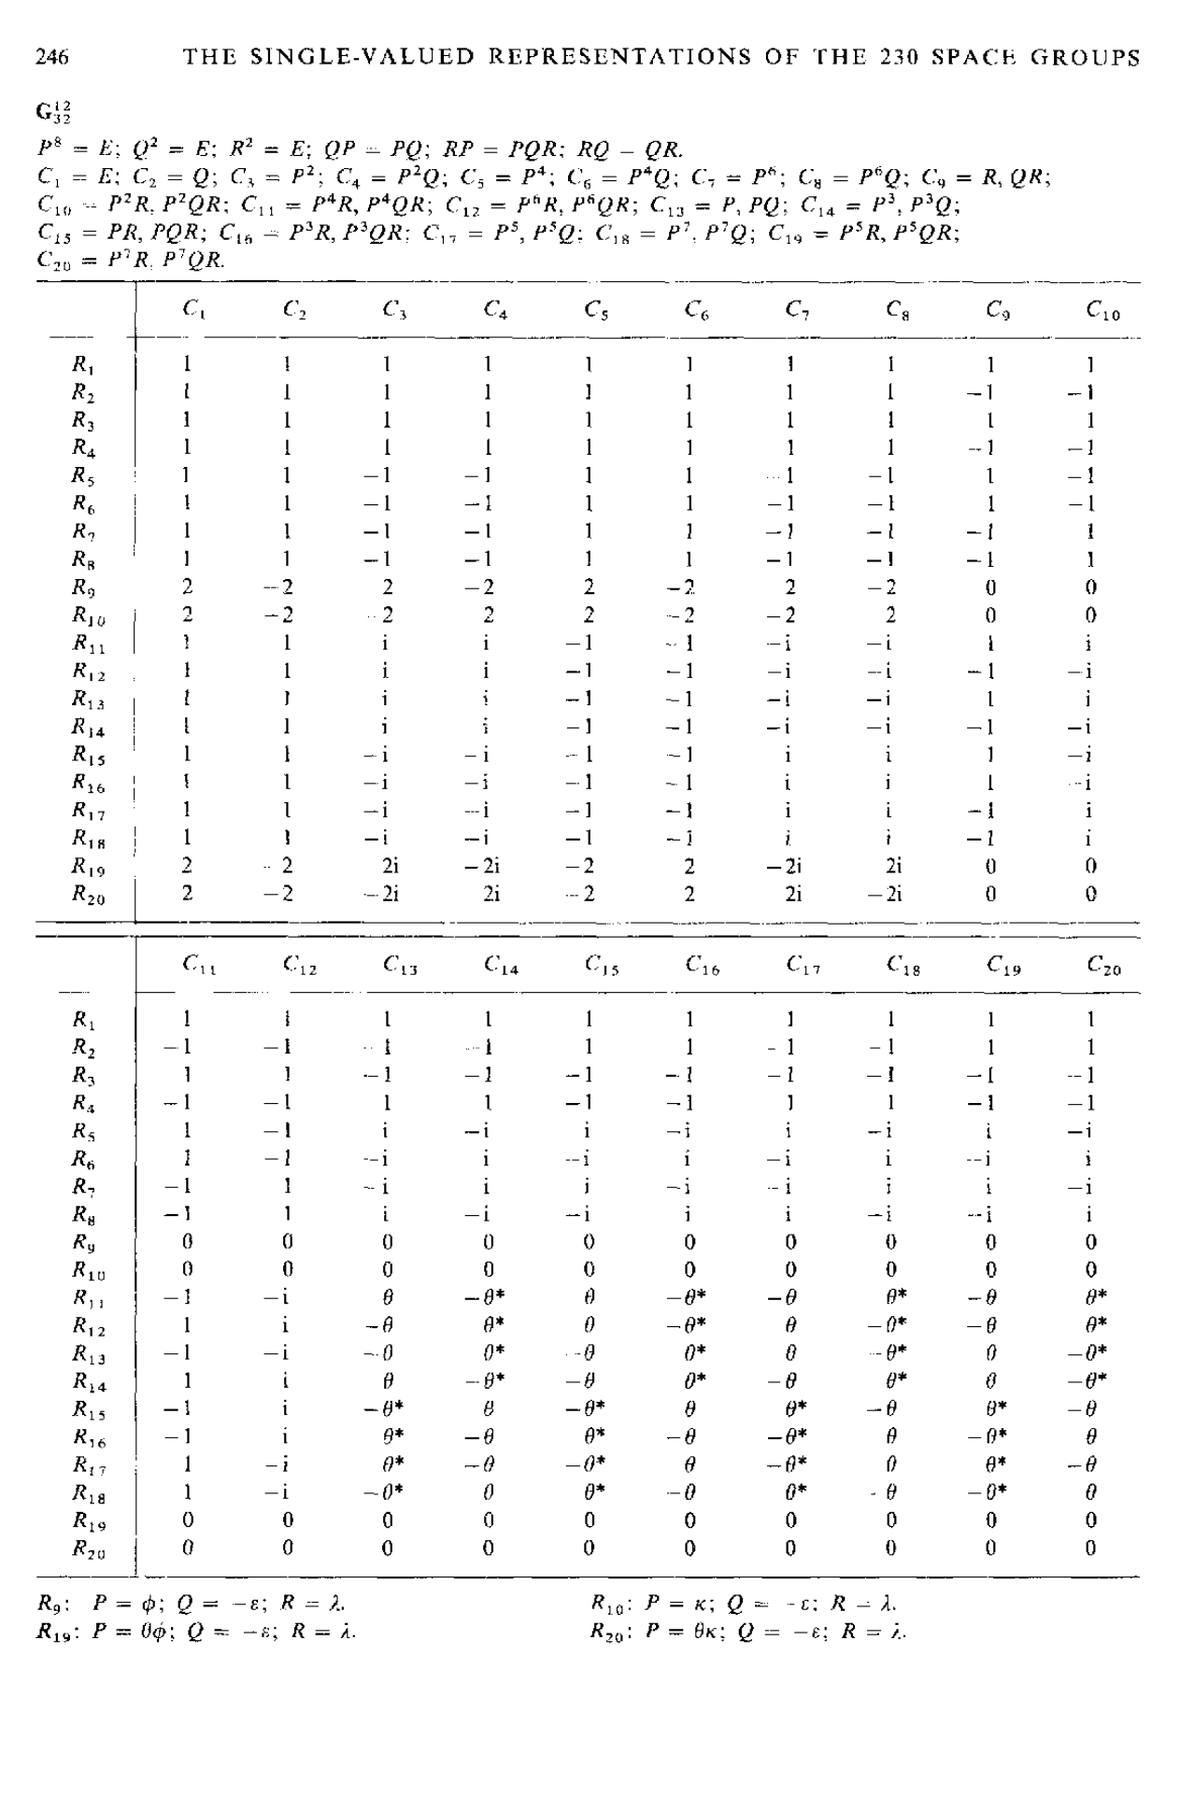
\includegraphics[width=0.86\textwidth]{c5_t51_p21.jpg}
\caption*{\textbf{表 5.1}（第 21 页，共 60 页；原书第 246 页）}
\end{figure}
\begin{figure}[H]
\centering
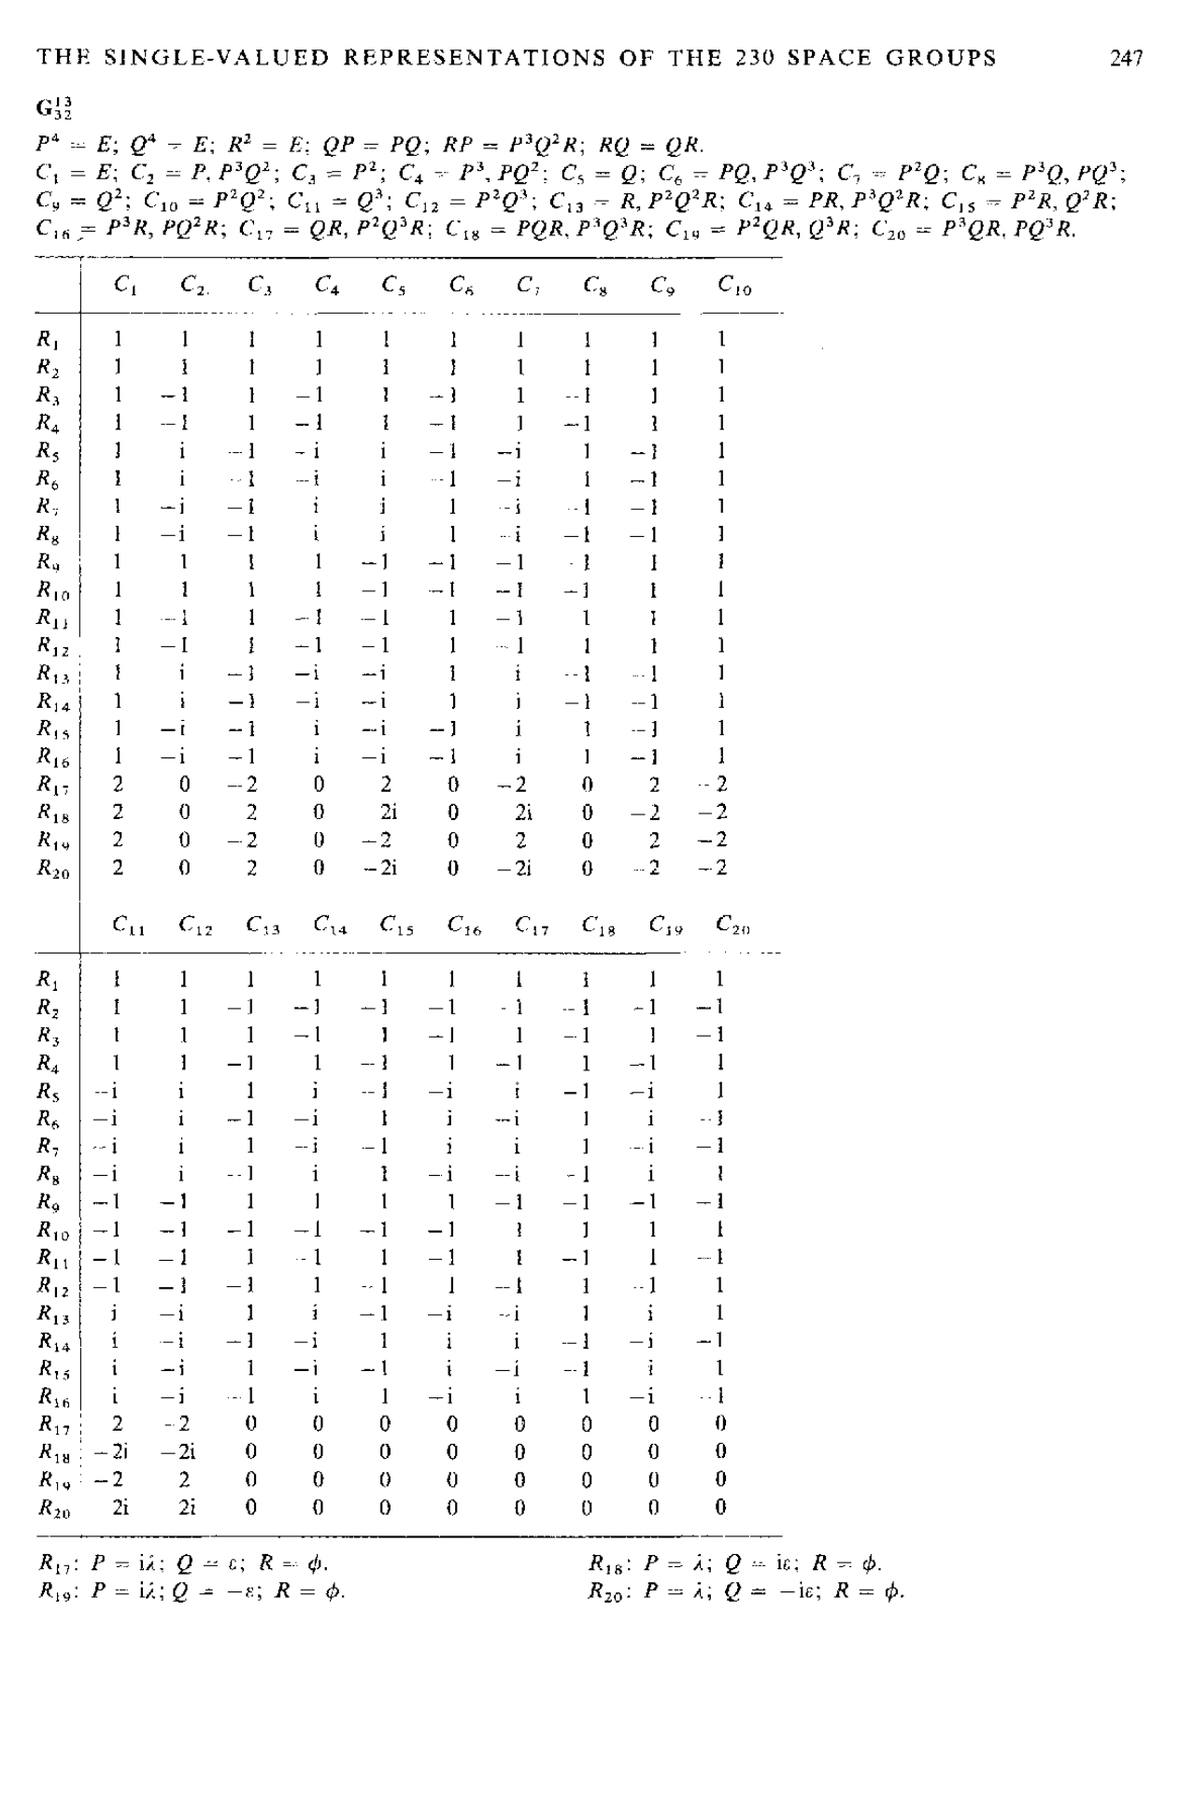
\includegraphics[width=0.86\textwidth]{c5_t51_p22.jpg}
\caption*{\textbf{表 5.1}（第 22 页，共 60 页；原书第 247 页）}
\end{figure}
\begin{figure}[H]
\centering
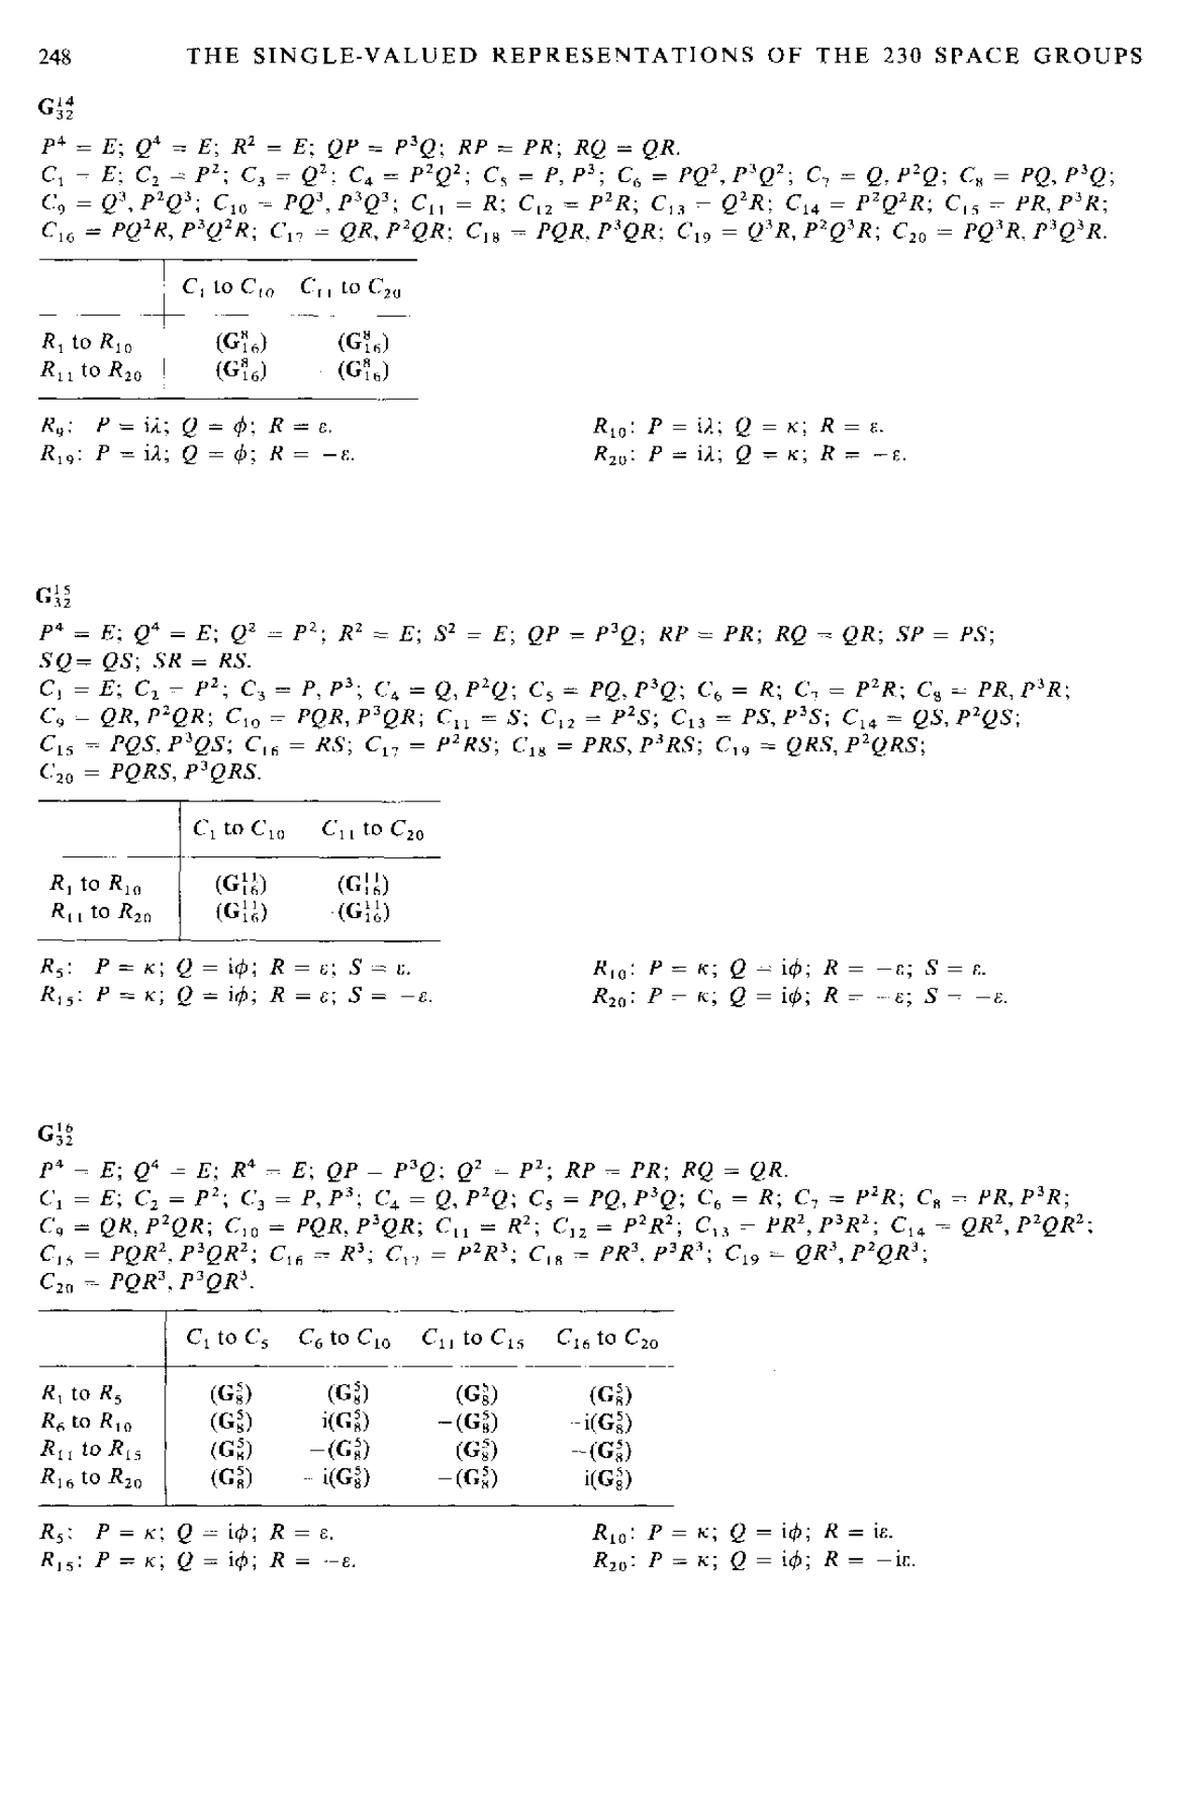
\includegraphics[width=0.86\textwidth]{c5_t51_p23.jpg}
\caption*{\textbf{表 5.1}（第 23 页，共 60 页；原书第 248 页）}
\end{figure}
\begin{figure}[H]
\centering
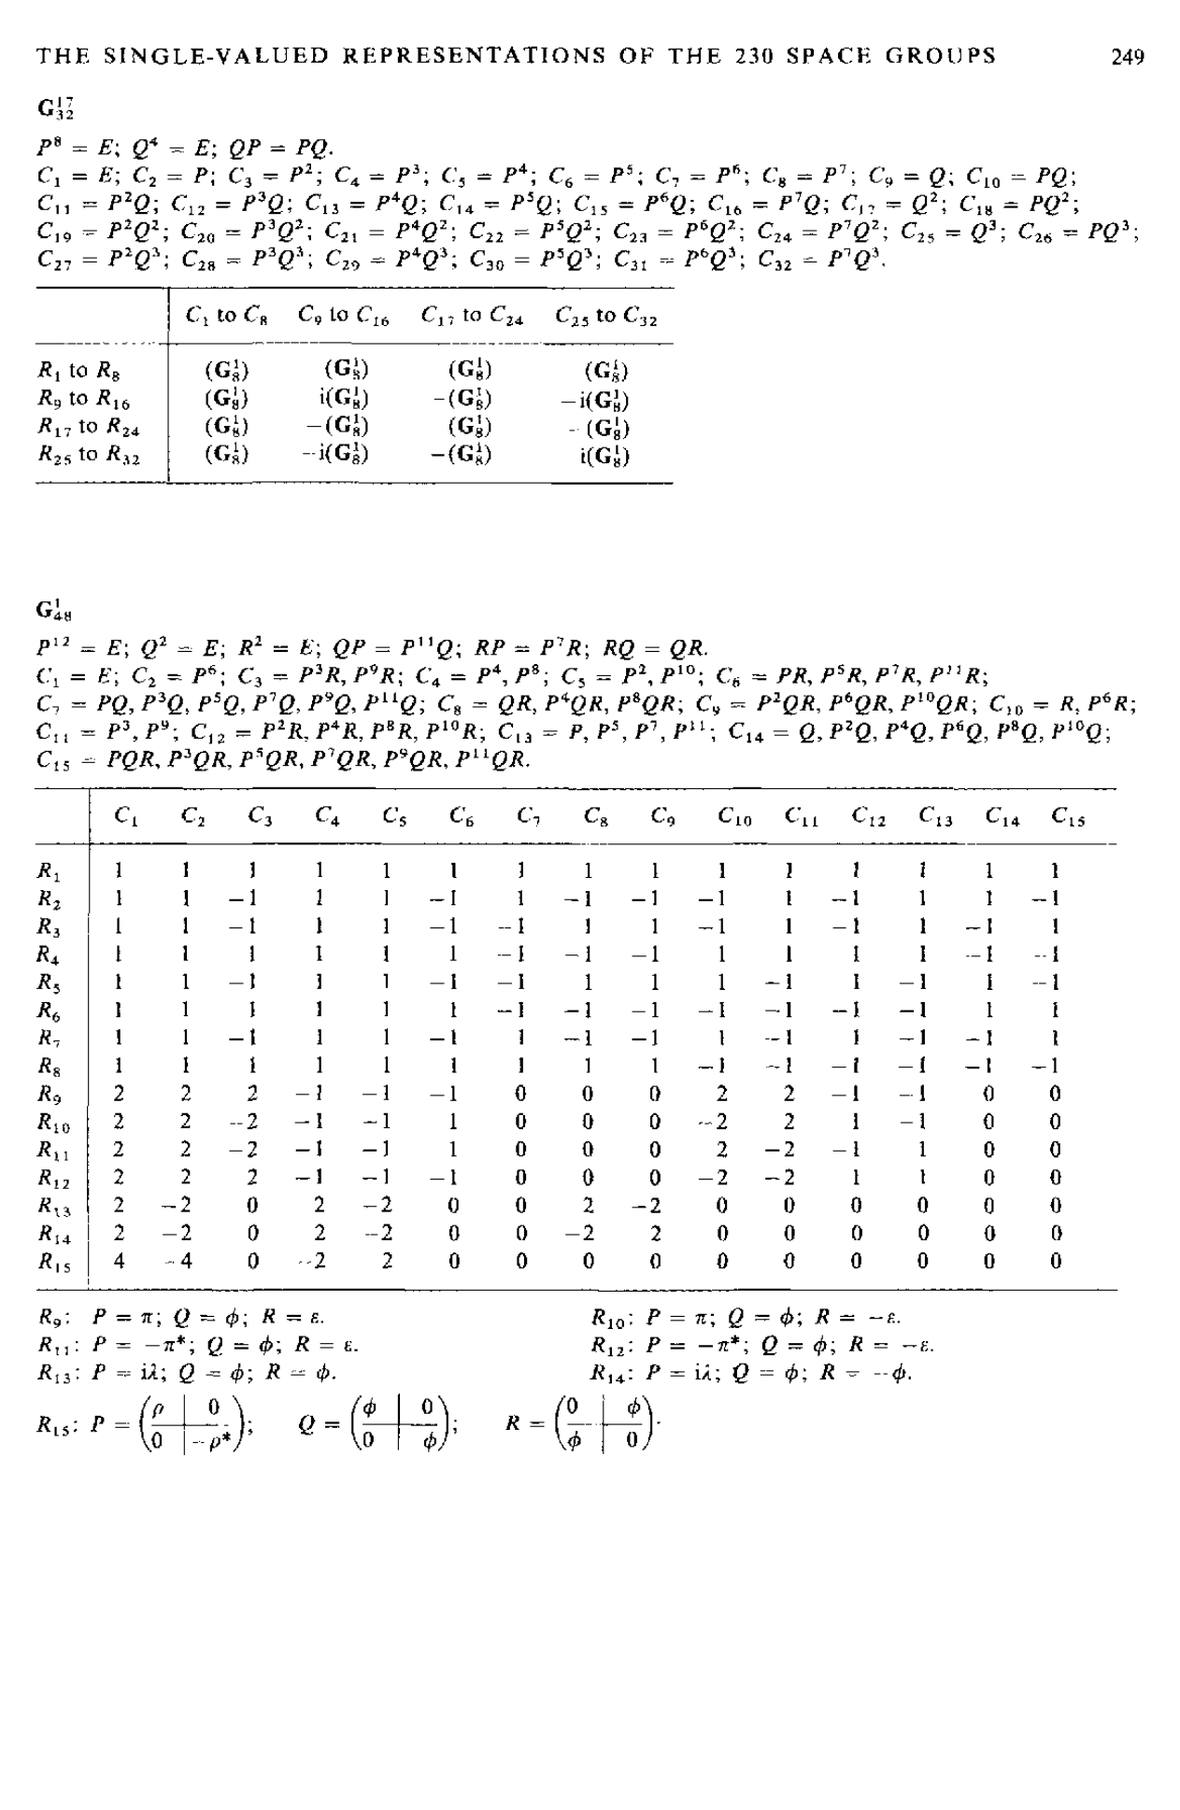
\includegraphics[width=0.86\textwidth]{c5_t51_p24.jpg}
\caption*{\textbf{表 5.1}（第 24 页，共 60 页；原书第 249 页）}
\end{figure}
\begin{figure}[H]
\centering
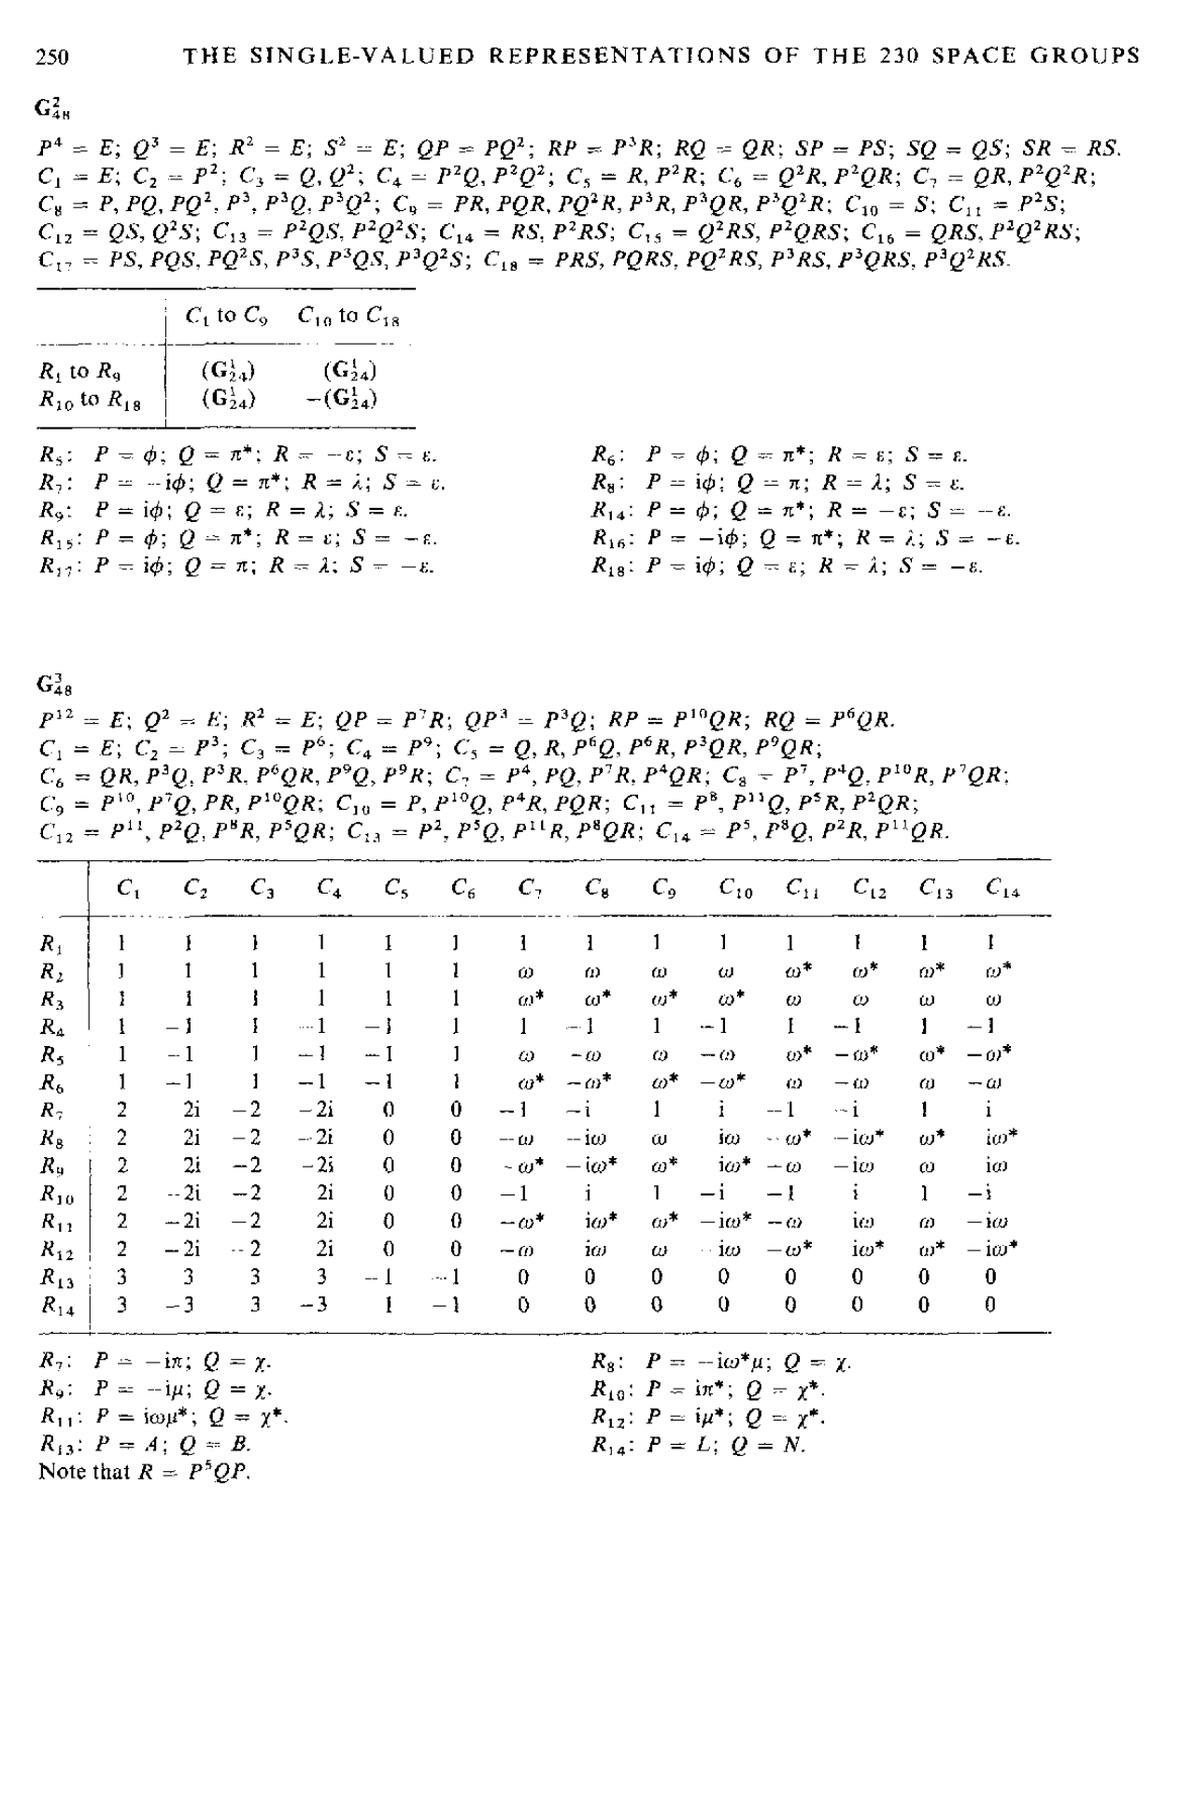
\includegraphics[width=0.86\textwidth]{c5_t51_p25.jpg}
\caption*{\textbf{表 5.1}（第 25 页，共 60 页；原书第 250 页）}
\end{figure}
\begin{figure}[H]
\centering
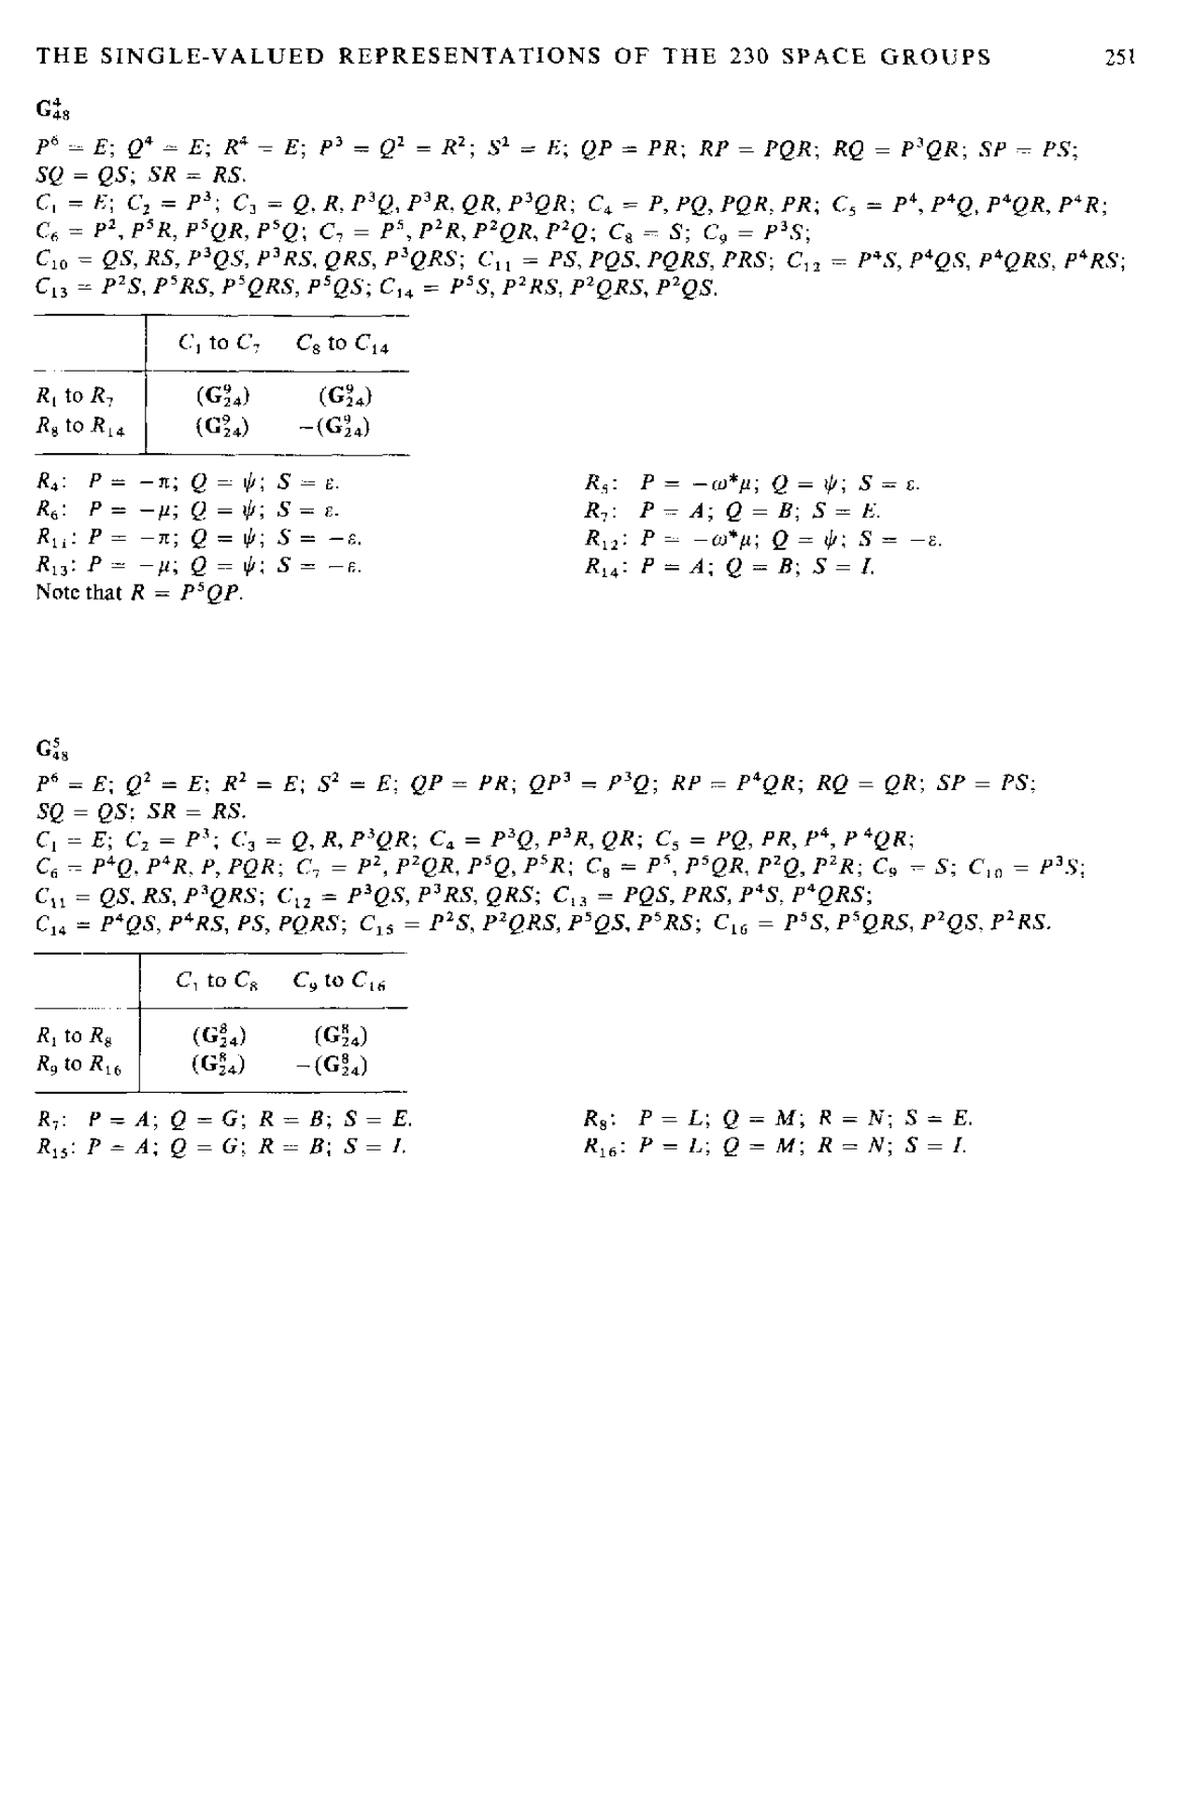
\includegraphics[width=0.86\textwidth]{c5_t51_p26.jpg}
\caption*{\textbf{表 5.1}（第 26 页，共 60 页；原书第 251 页）}
\end{figure}
\begin{figure}[H]
\centering
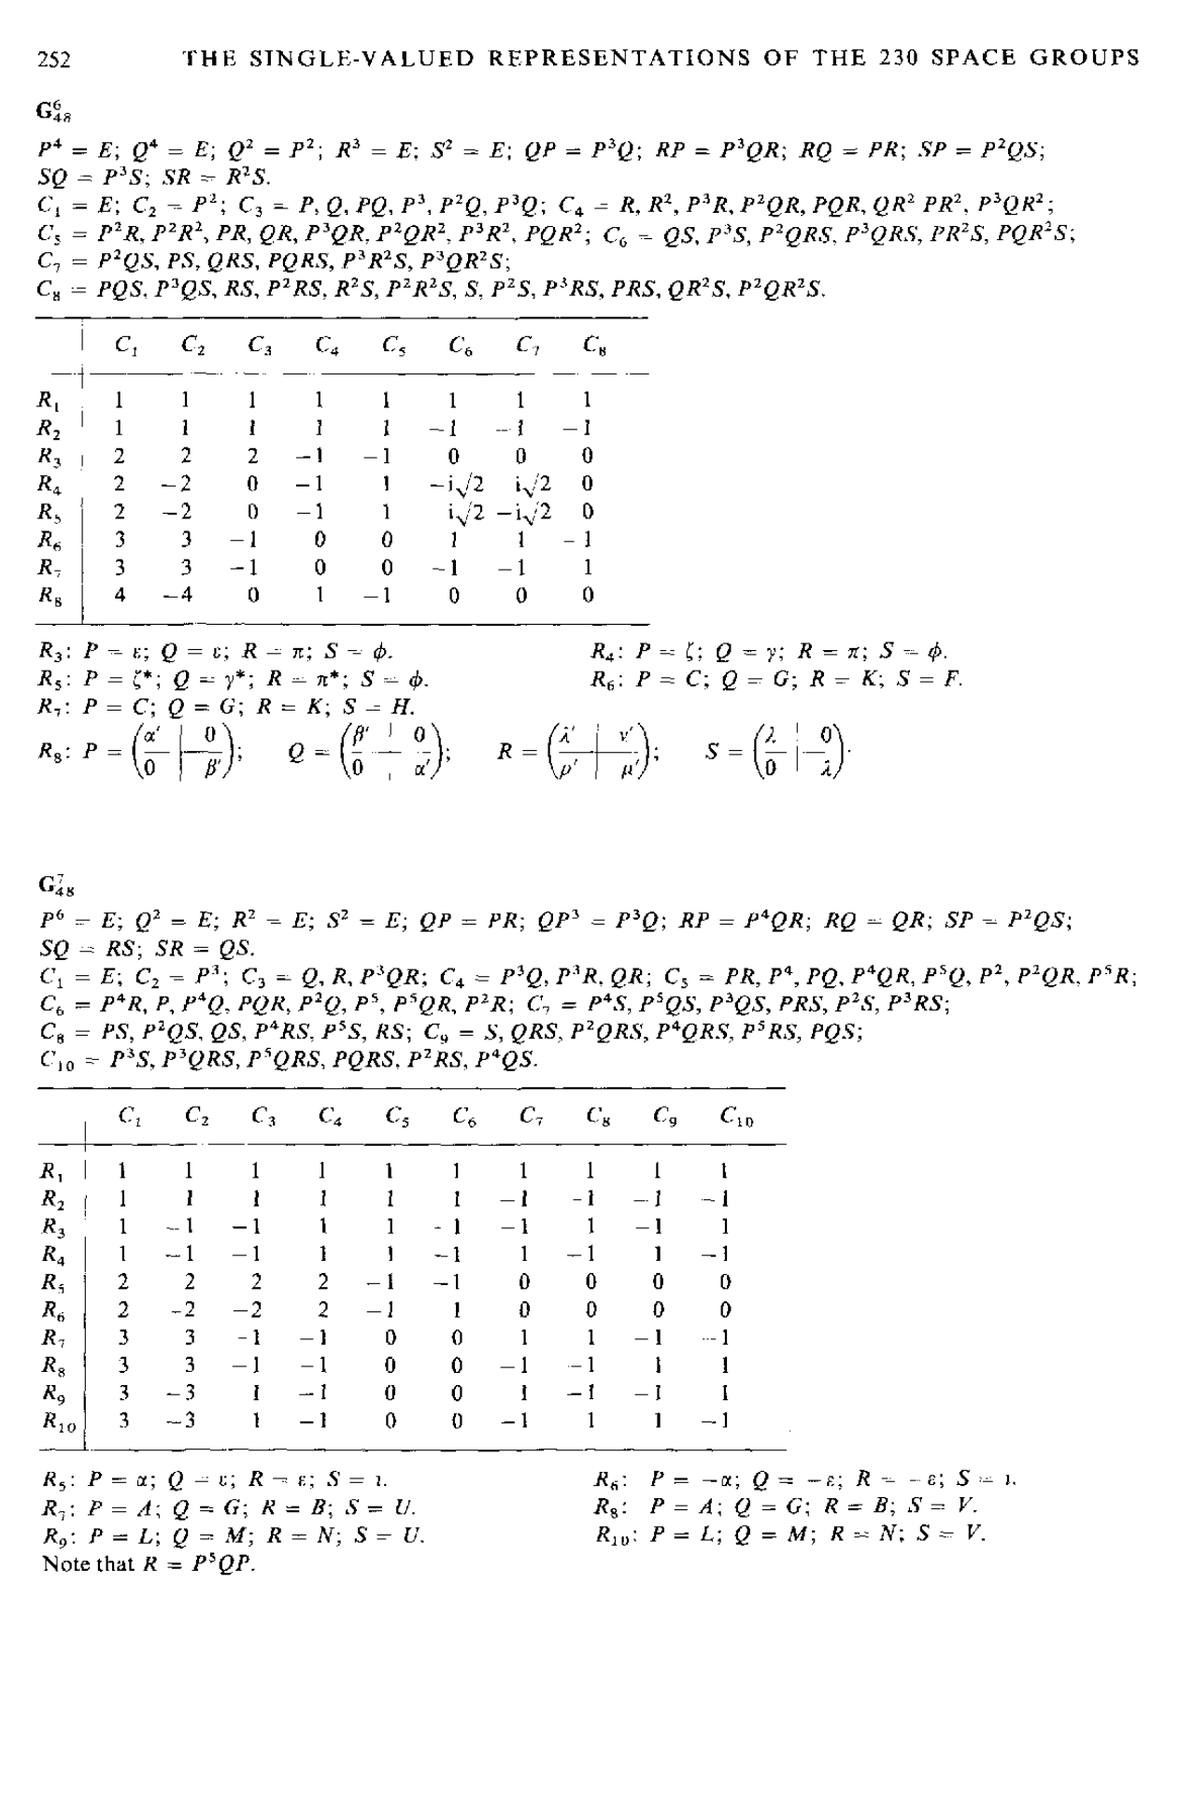
\includegraphics[width=0.86\textwidth]{c5_t51_p27.jpg}
\caption*{\textbf{表 5.1}（第 27 页，共 60 页；原书第 252 页）}
\end{figure}
\begin{figure}[H]
\centering
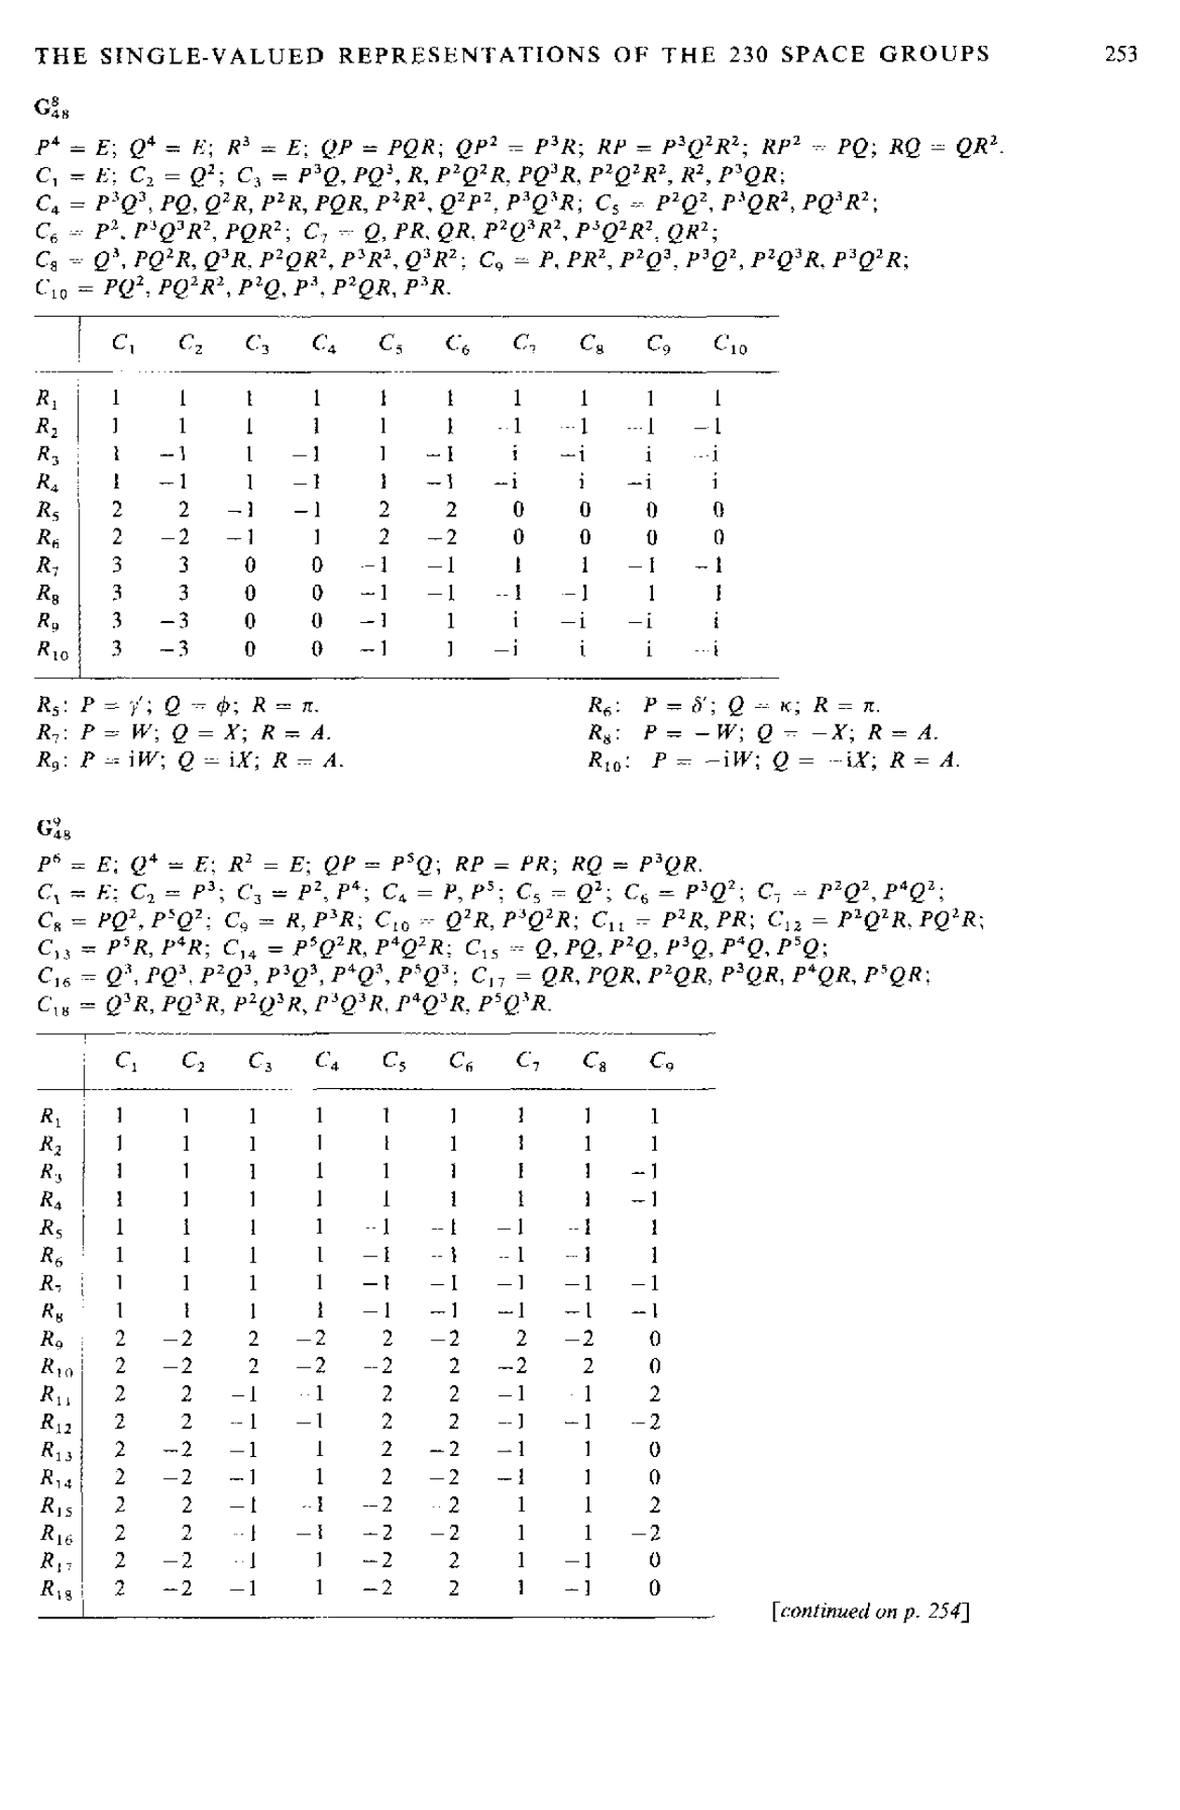
\includegraphics[width=0.86\textwidth]{c5_t51_p28.jpg}
\caption*{\textbf{表 5.1}（第 28 页，共 60 页；原书第 253 页）}
\end{figure}
\begin{figure}[H]
\centering
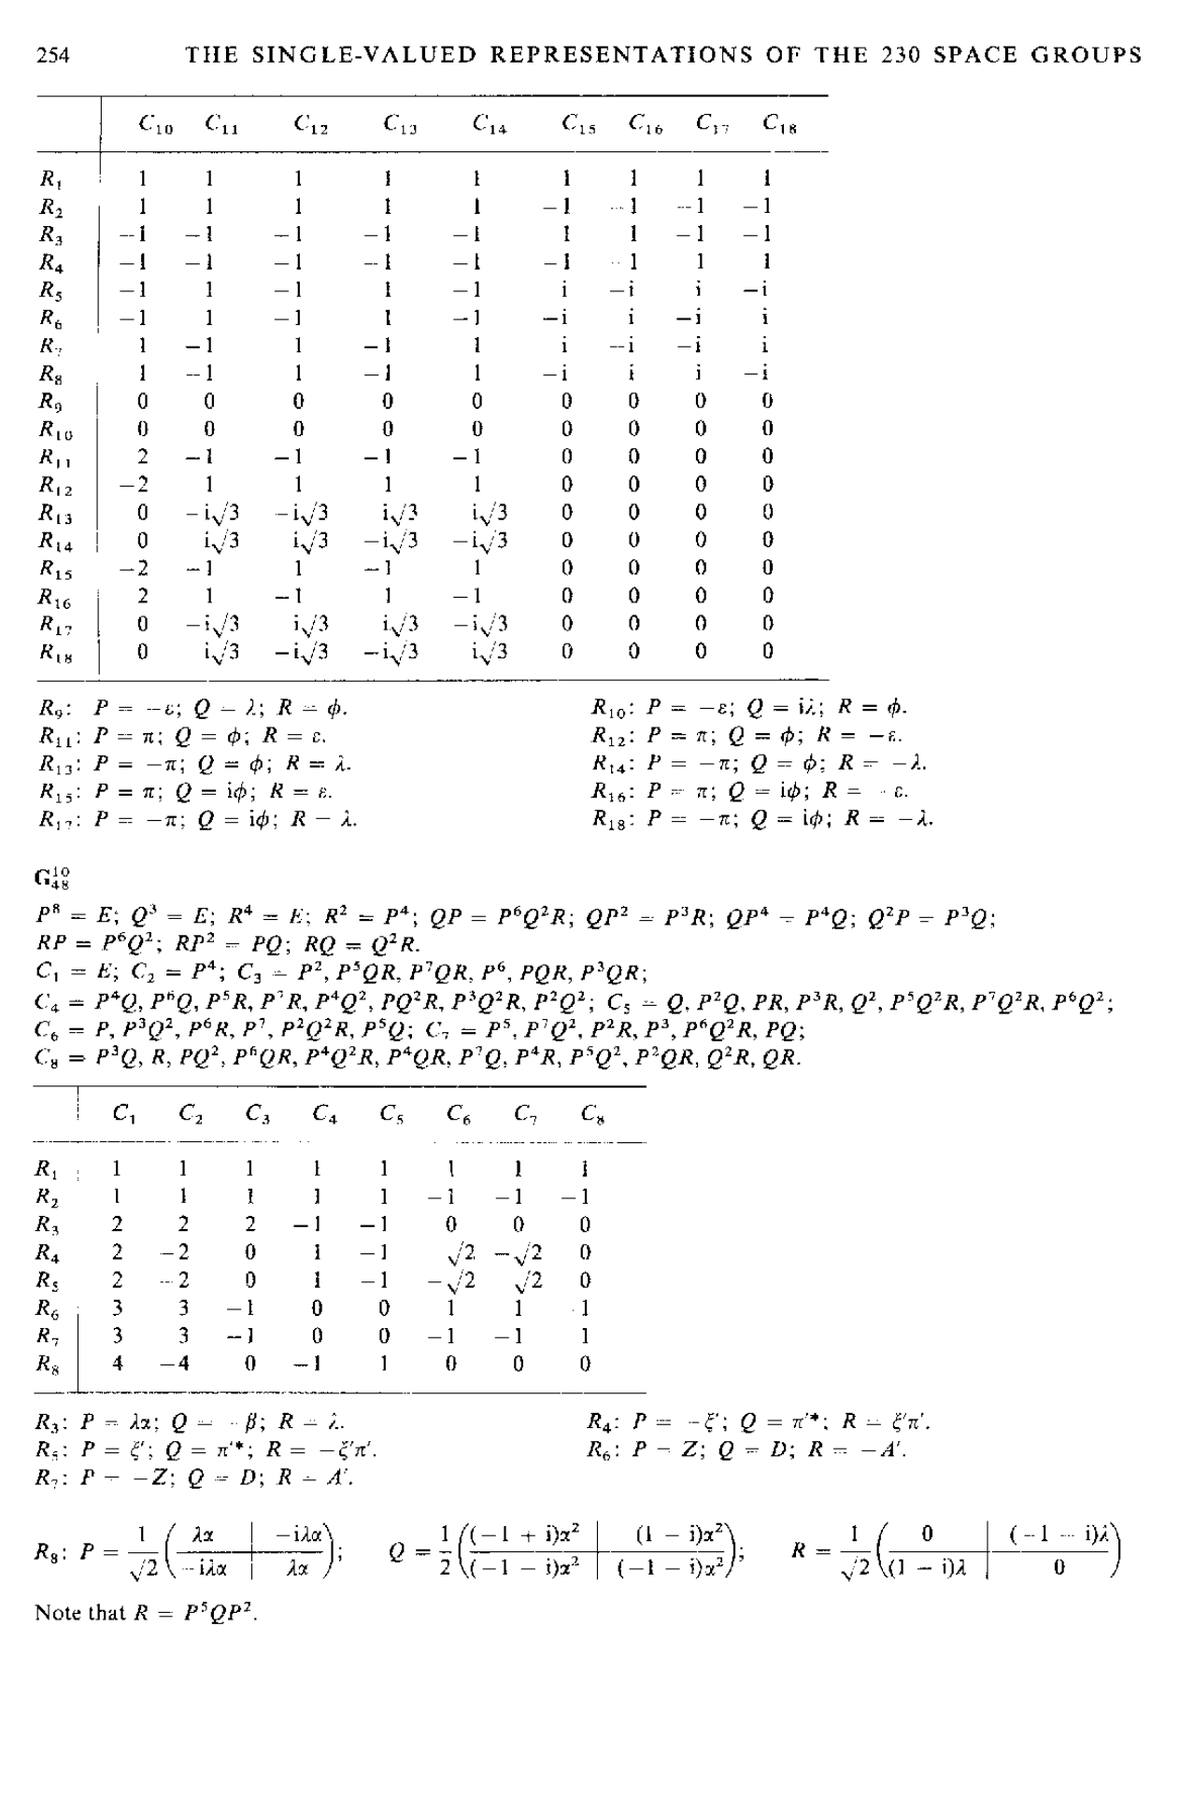
\includegraphics[width=0.86\textwidth]{c5_t51_p29.jpg}
\caption*{\textbf{表 5.1}（第 29 页，共 60 页；原书第 254 页）}
\end{figure}
\begin{figure}[H]
\centering
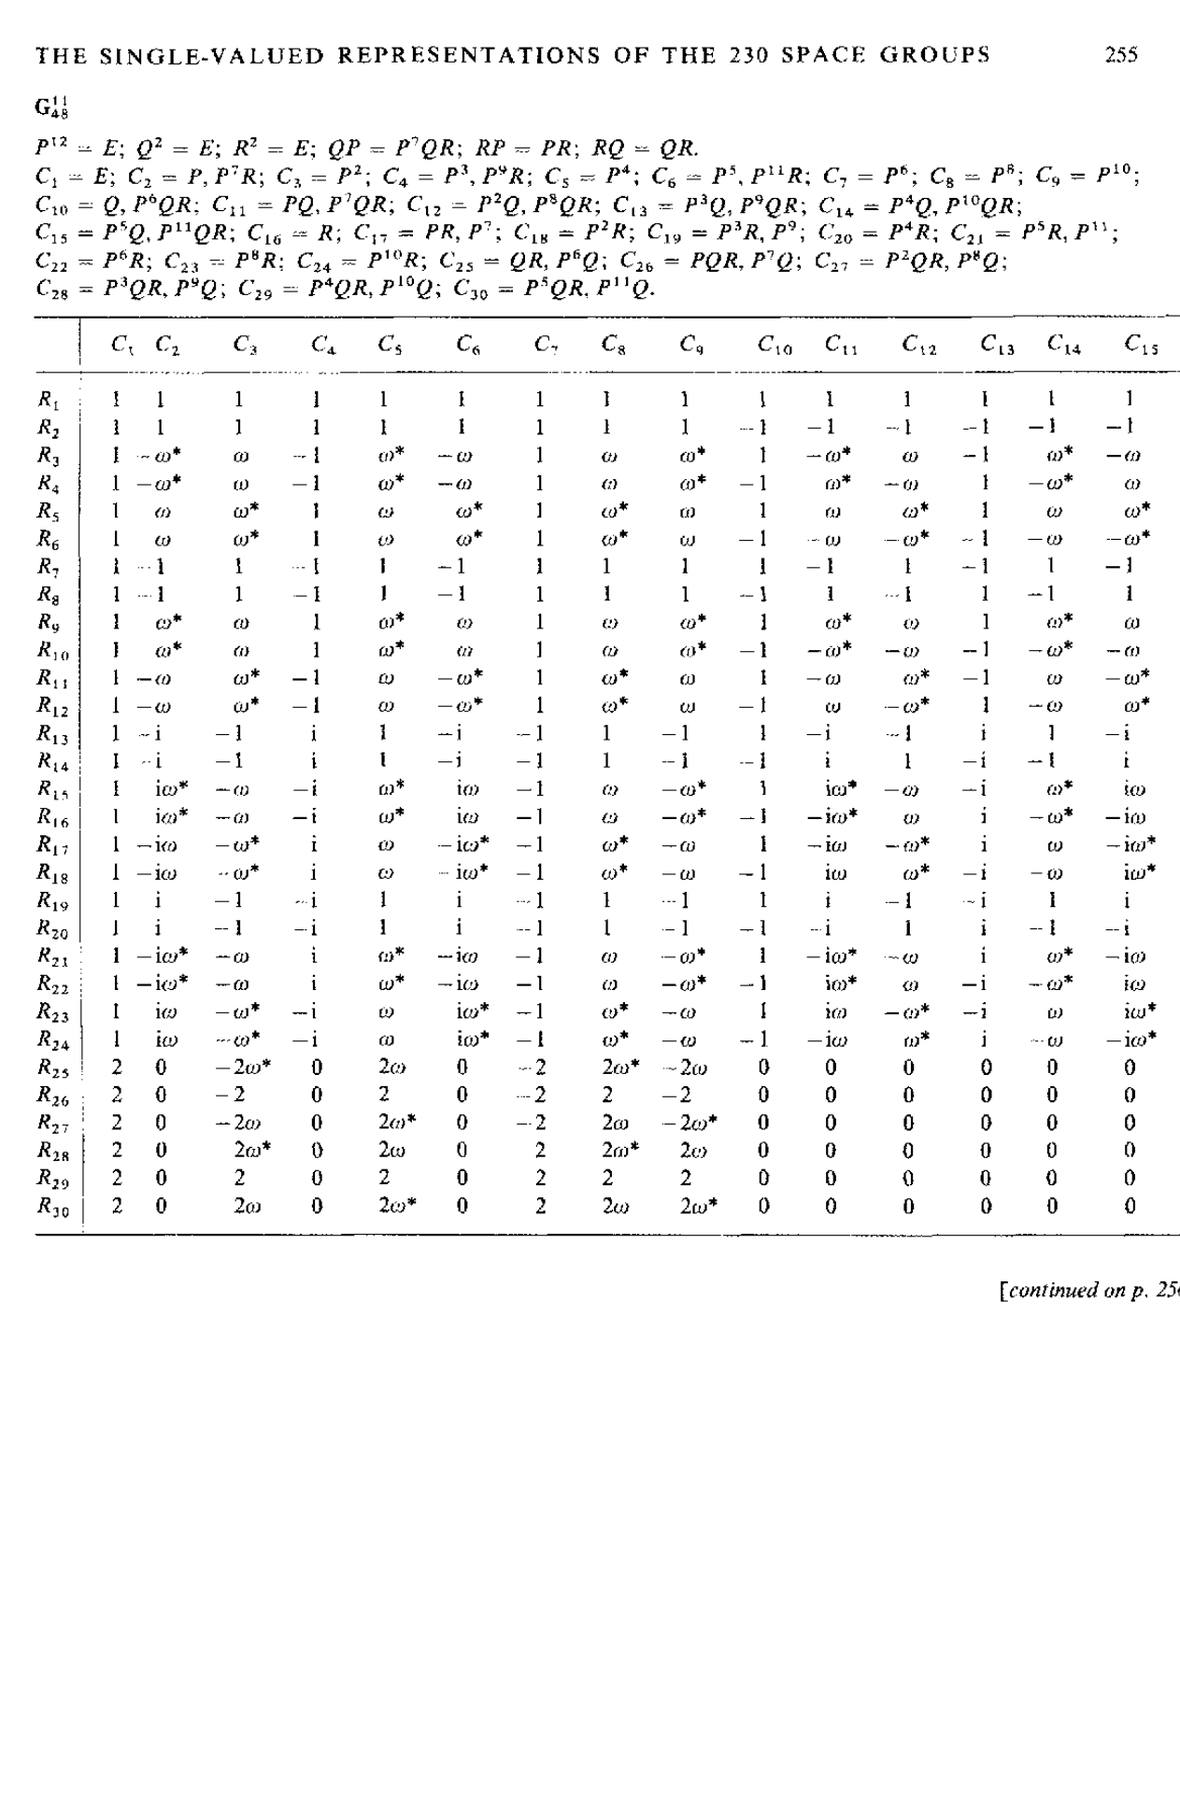
\includegraphics[width=0.86\textwidth]{c5_t51_p30.jpg}
\caption*{\textbf{表 5.1}（第 30 页，共 60 页；原书第 255 页）}
\end{figure}
\begin{figure}[H]
\centering
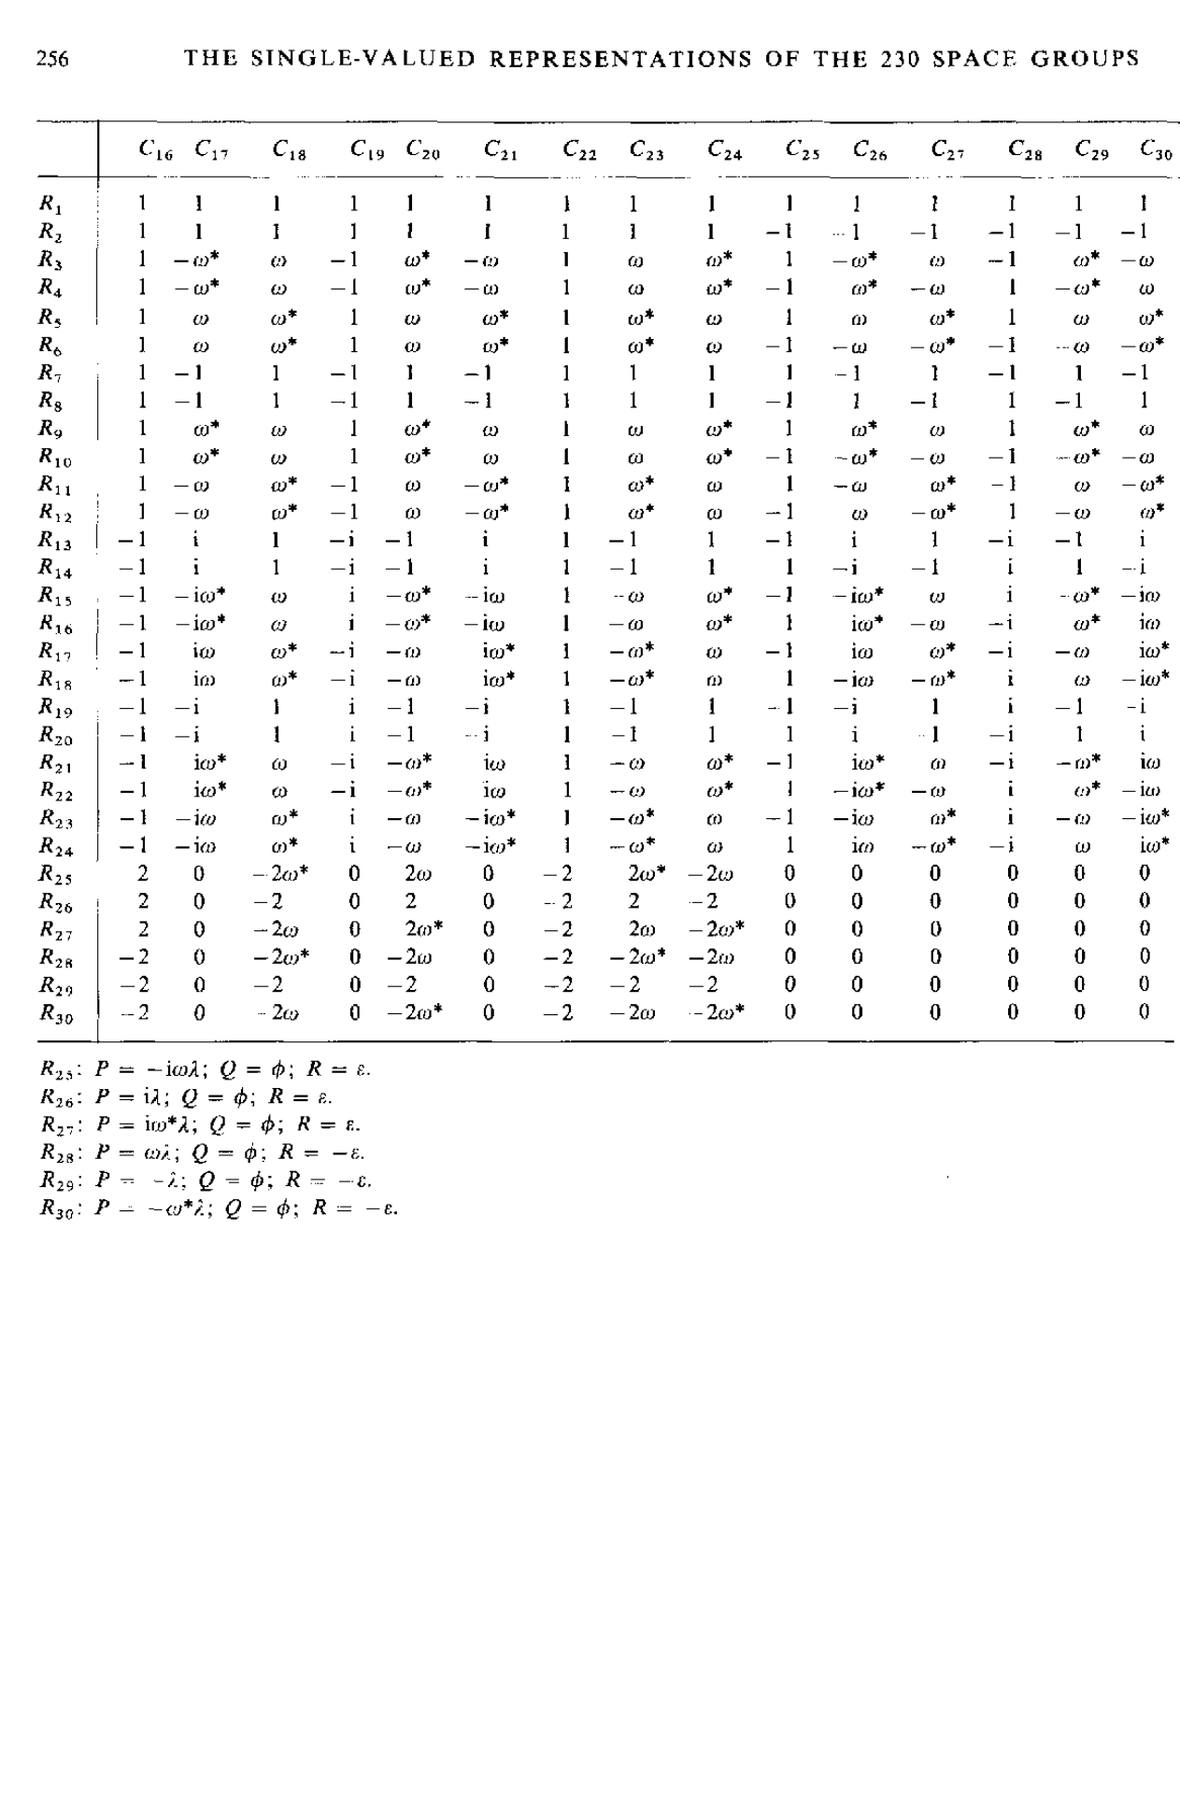
\includegraphics[width=0.86\textwidth]{c5_t51_p31.jpg}
\caption*{\textbf{表 5.1}（第 31 页，共 60 页；原书第 256 页）}
\end{figure}
\begin{figure}[H]
\centering
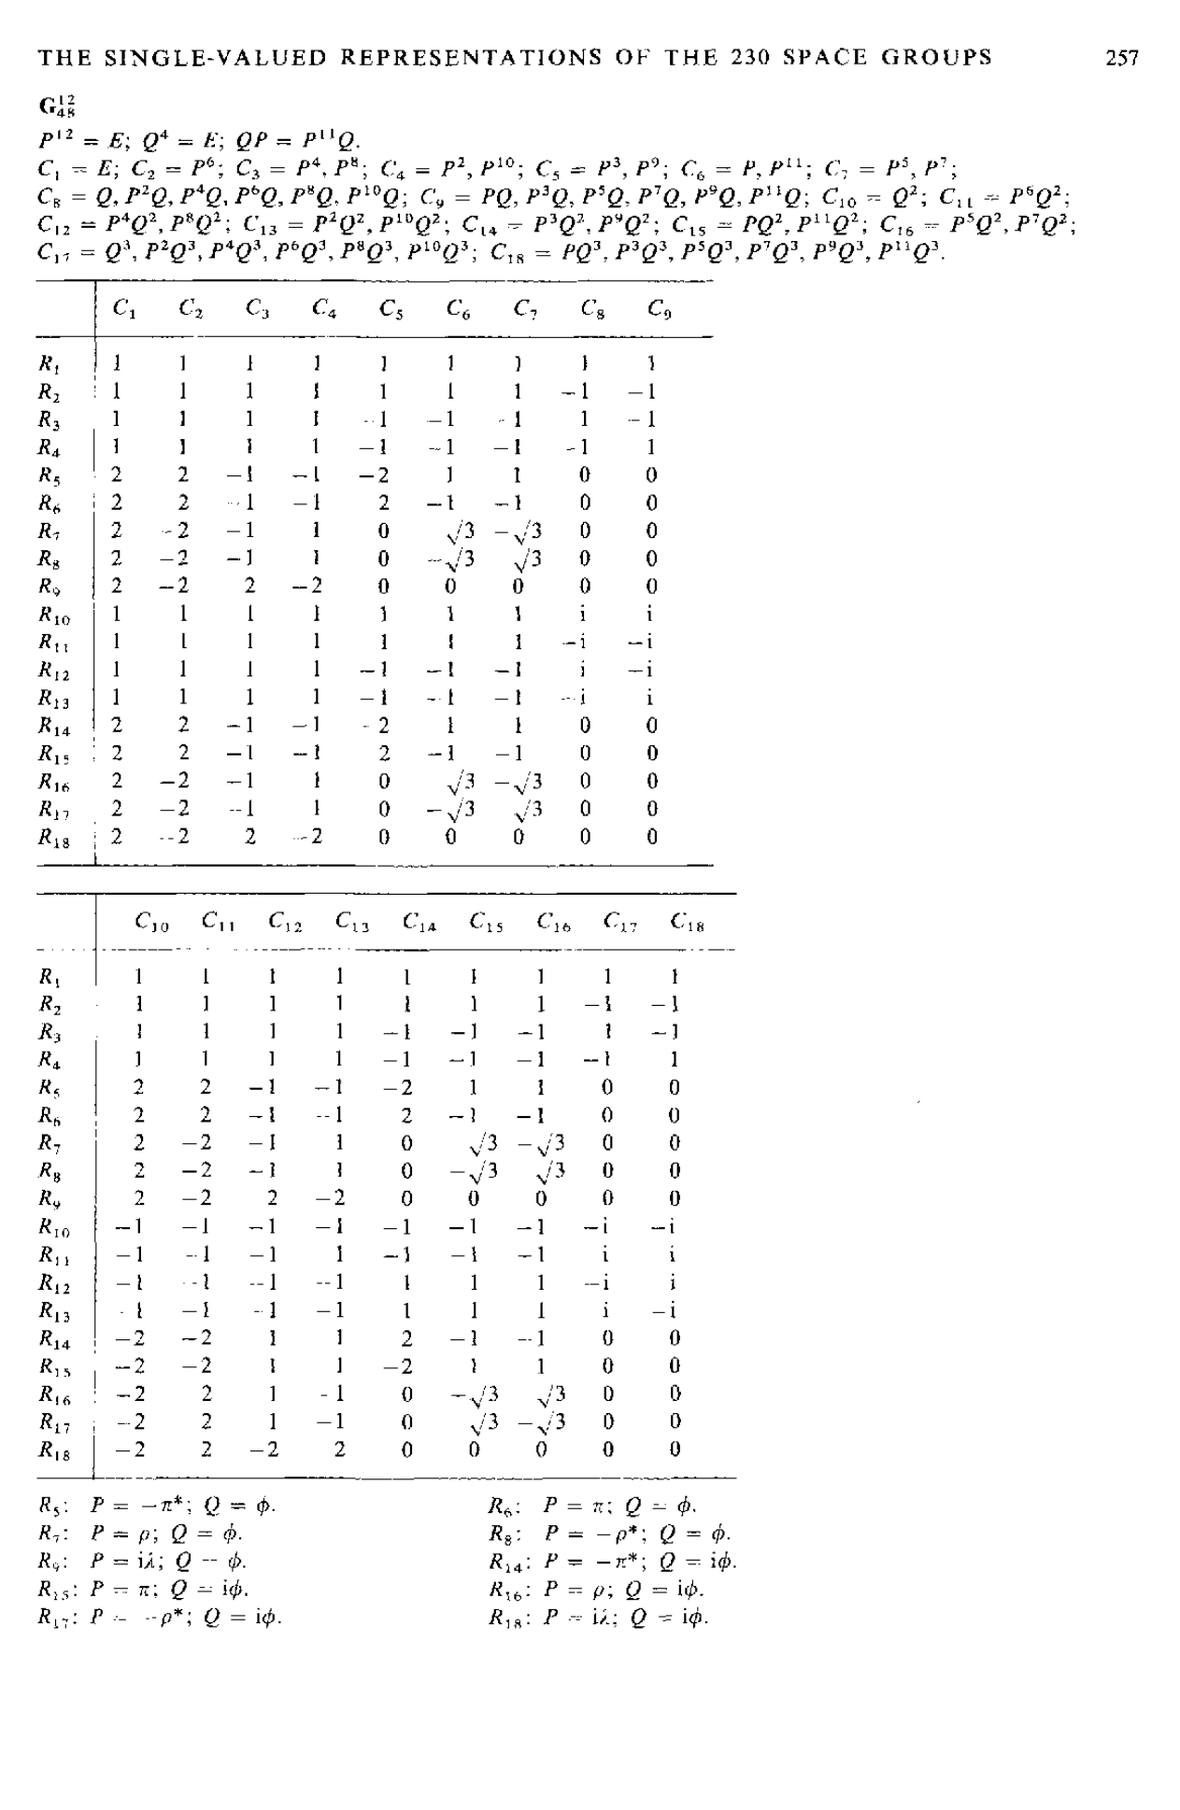
\includegraphics[width=0.86\textwidth]{c5_t51_p32.jpg}
\caption*{\textbf{表 5.1}（第 32 页，共 60 页；原书第 257 页）}
\end{figure}
\begin{figure}[H]
\centering
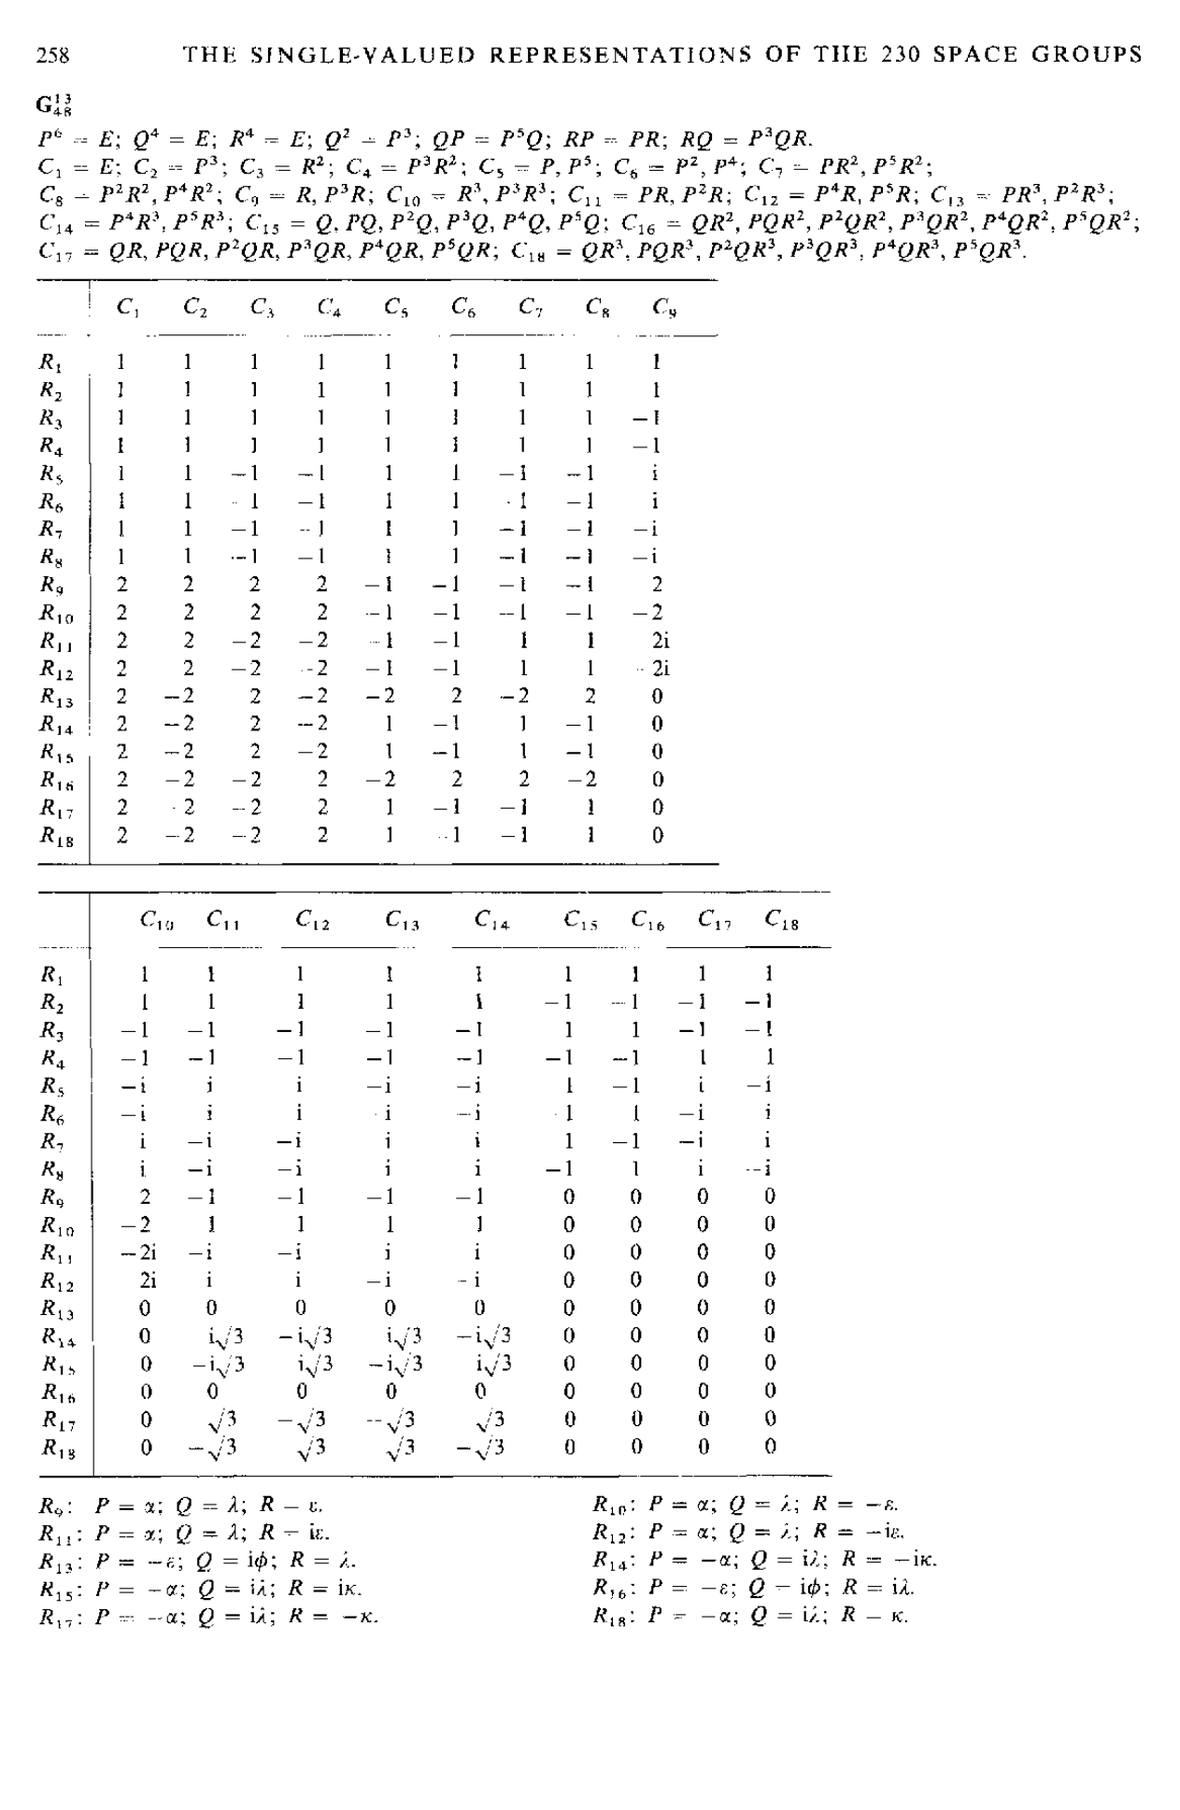
\includegraphics[width=0.86\textwidth]{c5_t51_p33.jpg}
\caption*{\textbf{表 5.1}（第 33 页，共 60 页；原书第 258 页）}
\end{figure}
\begin{figure}[H]
\centering
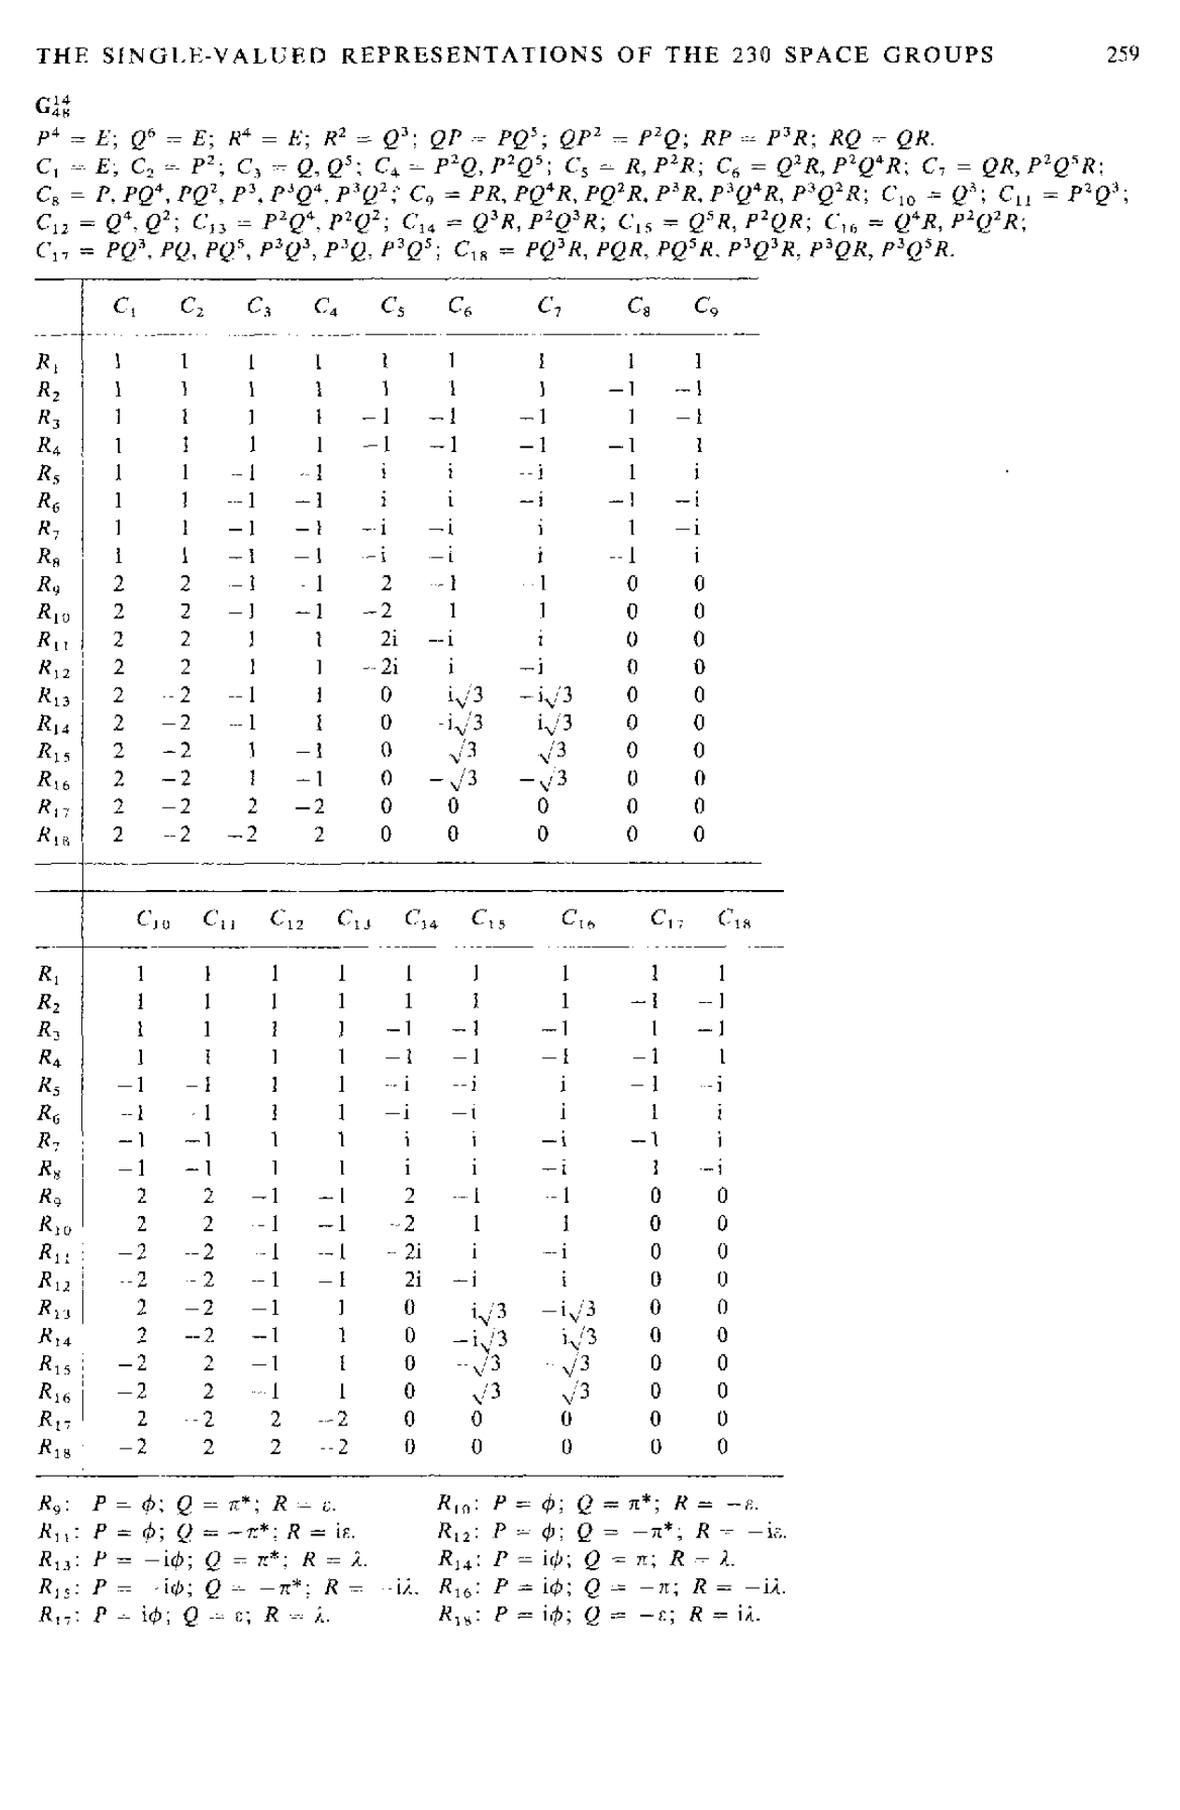
\includegraphics[width=0.86\textwidth]{c5_t51_p34.jpg}
\caption*{\textbf{表 5.1}（第 34 页，共 60 页；原书第 259 页）}
\end{figure}
\begin{figure}[H]
\centering
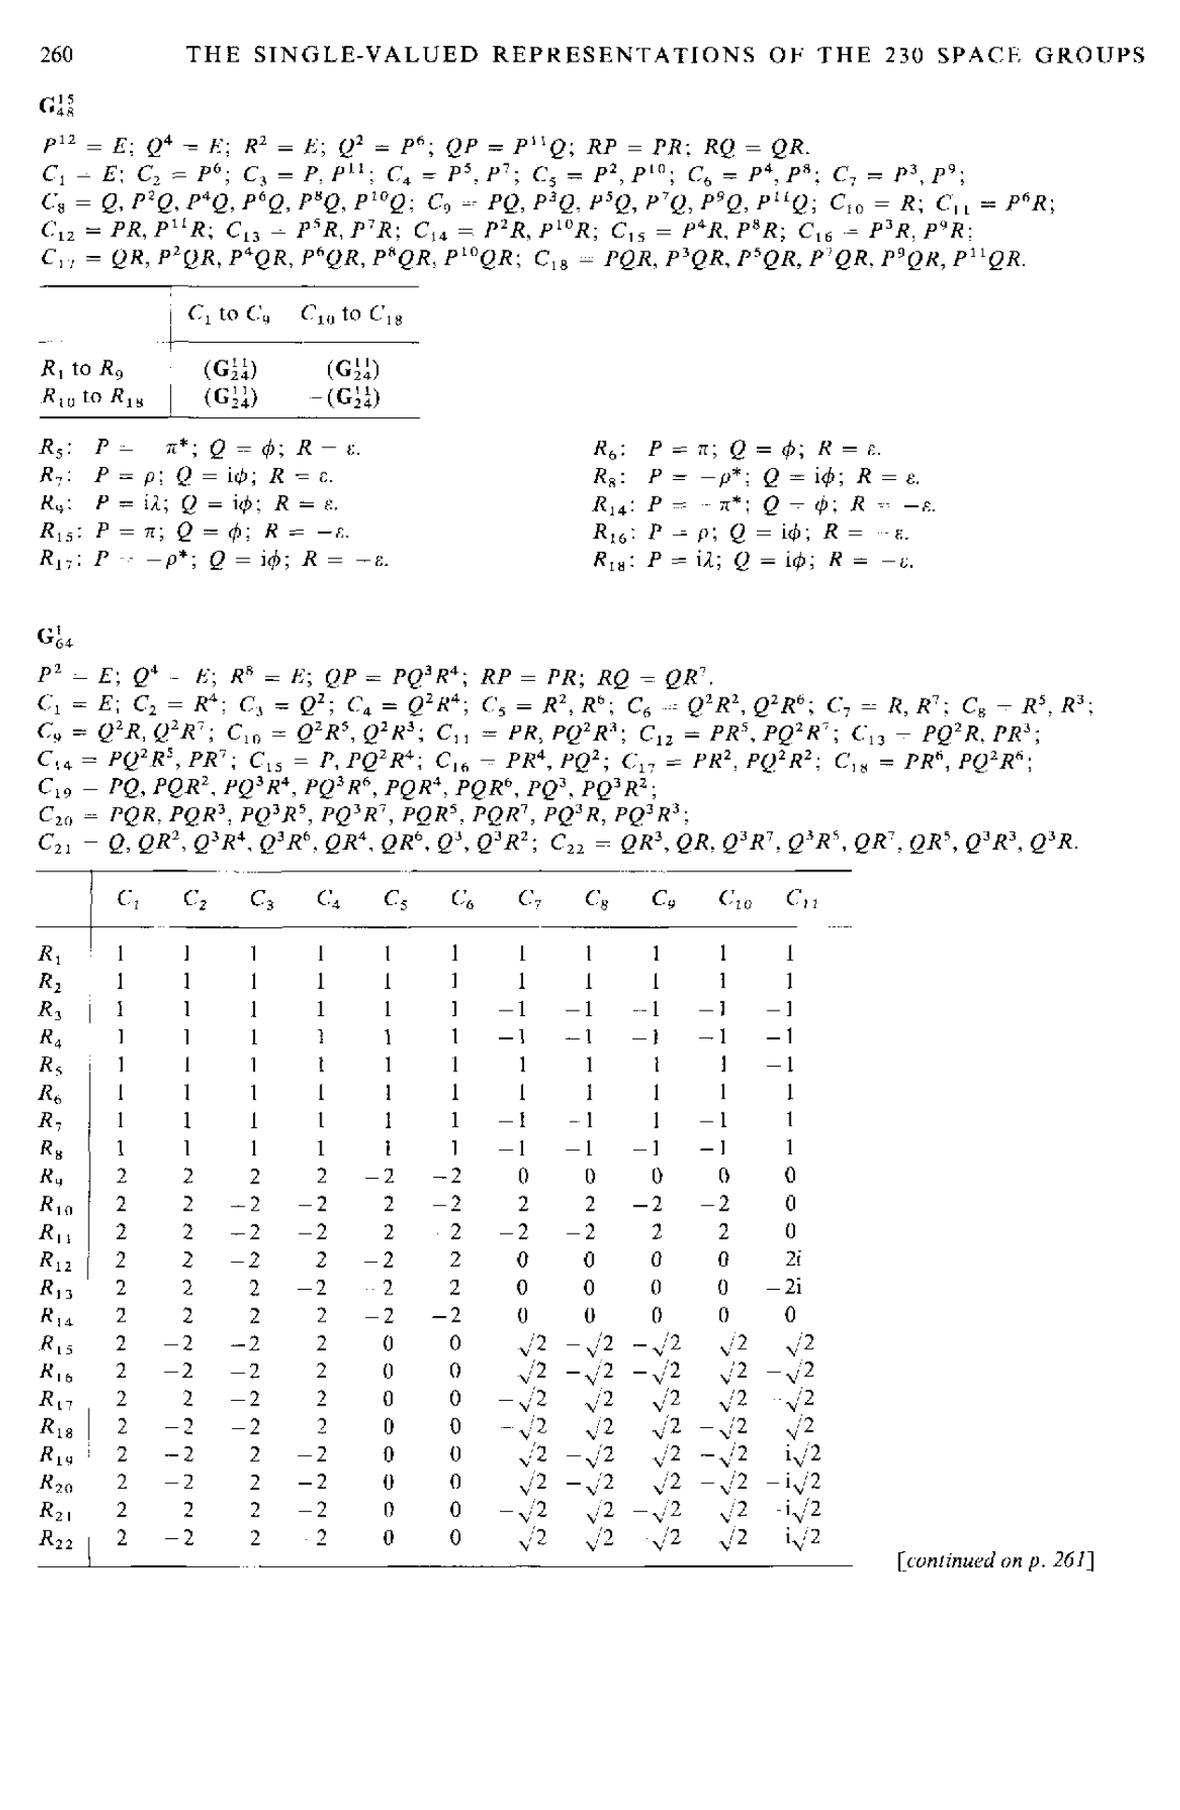
\includegraphics[width=0.86\textwidth]{c5_t51_p35.jpg}
\caption*{\textbf{表 5.1}（第 35 页，共 60 页；原书第 260 页）}
\end{figure}
\begin{figure}[H]
\centering
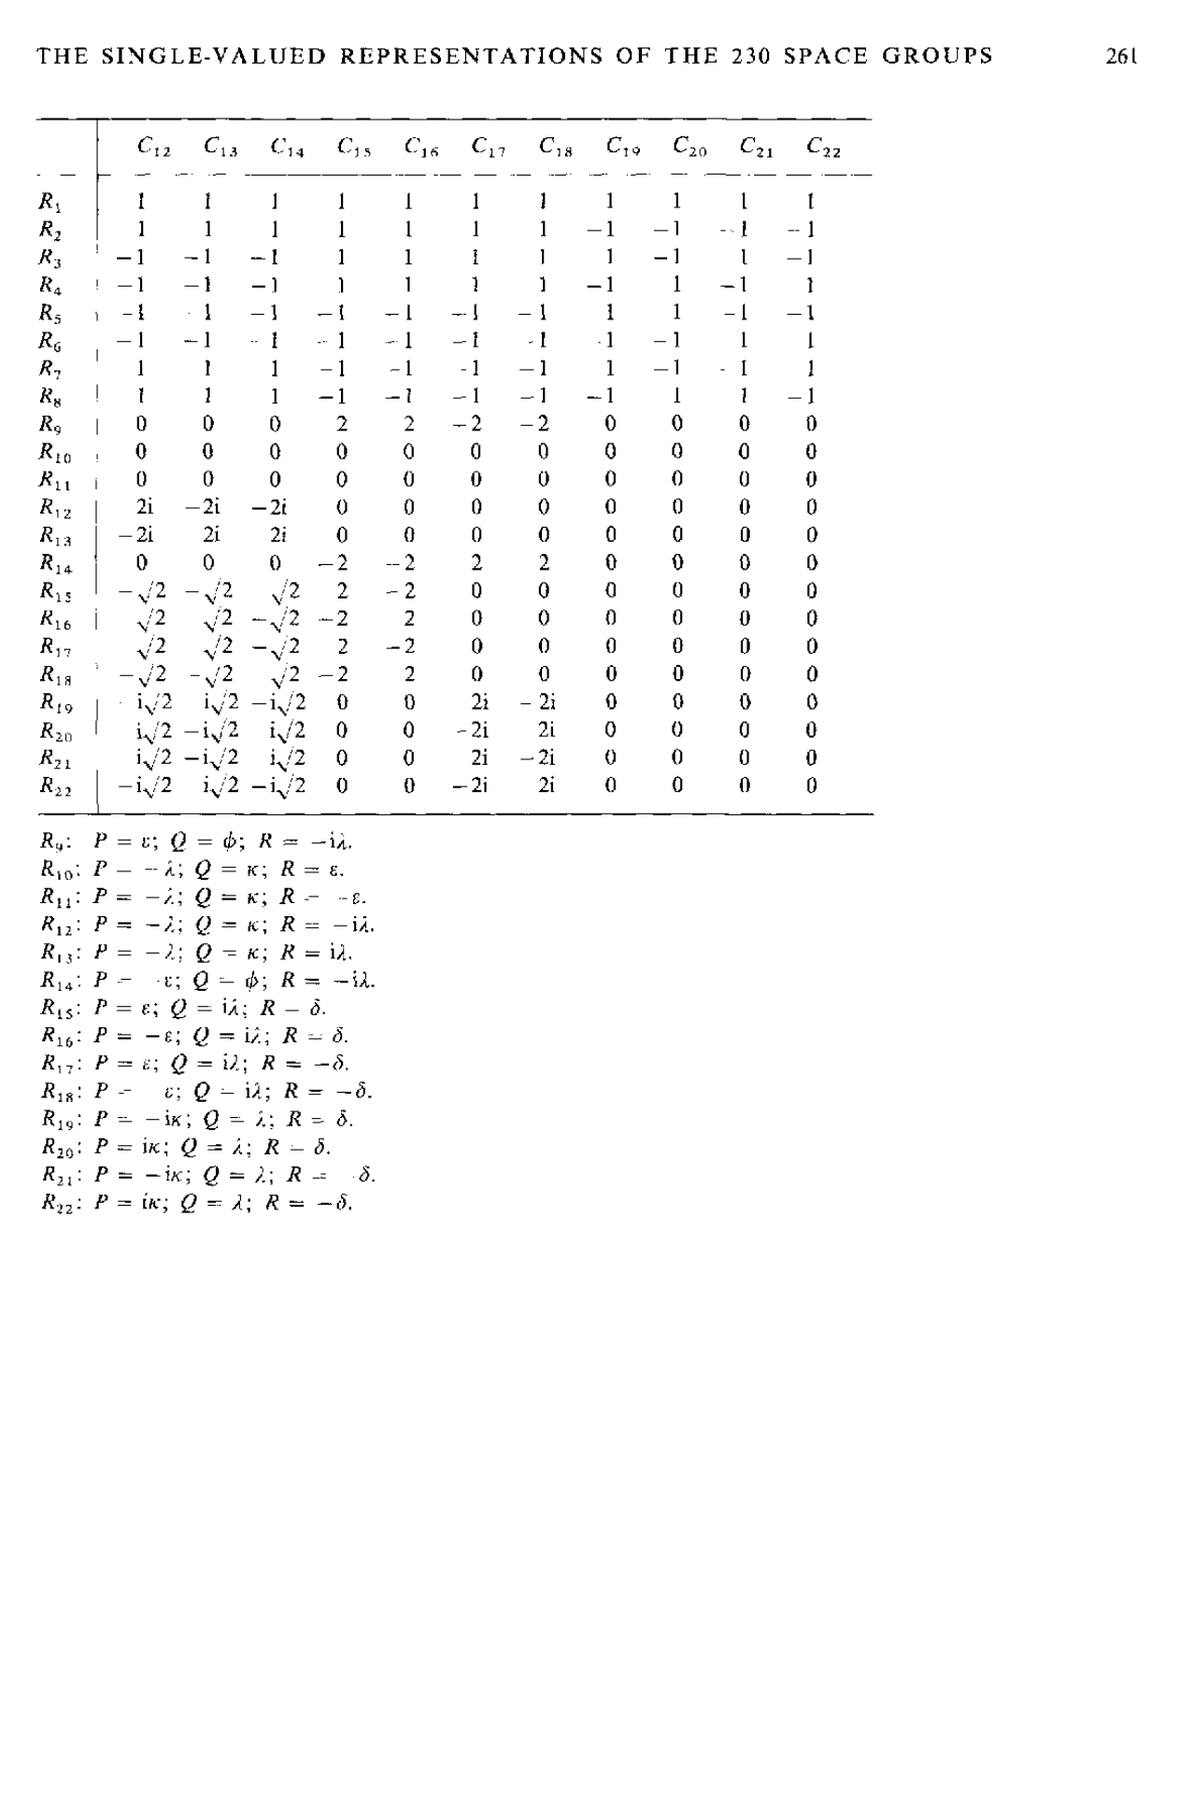
\includegraphics[width=0.86\textwidth]{c5_t51_p36.jpg}
\caption*{\textbf{表 5.1}（第 36 页，共 60 页；原书第 261 页）}
\end{figure}
\begin{figure}[H]
\centering
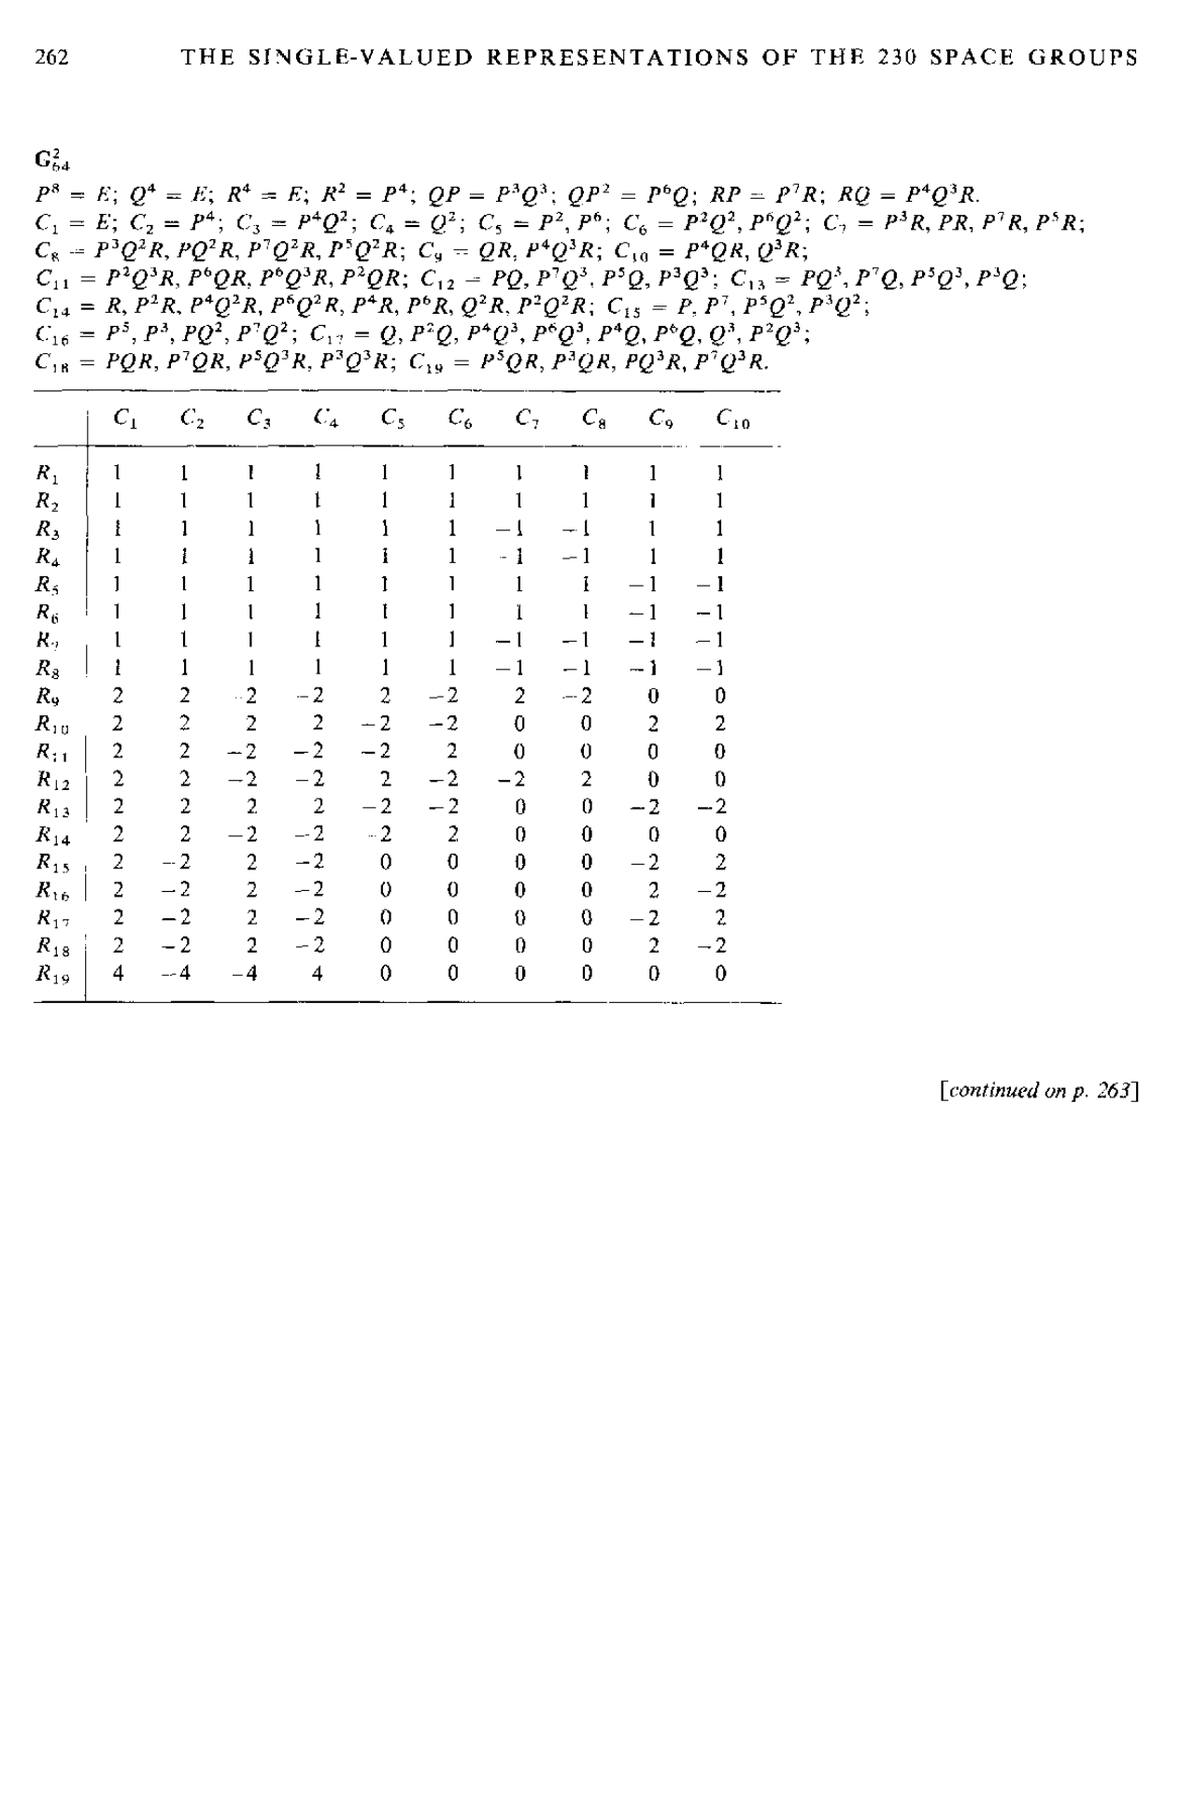
\includegraphics[width=0.86\textwidth]{c5_t51_p37.jpg}
\caption*{\textbf{表 5.1}（第 37 页，共 60 页；原书第 262 页）}
\end{figure}
\begin{figure}[H]
\centering
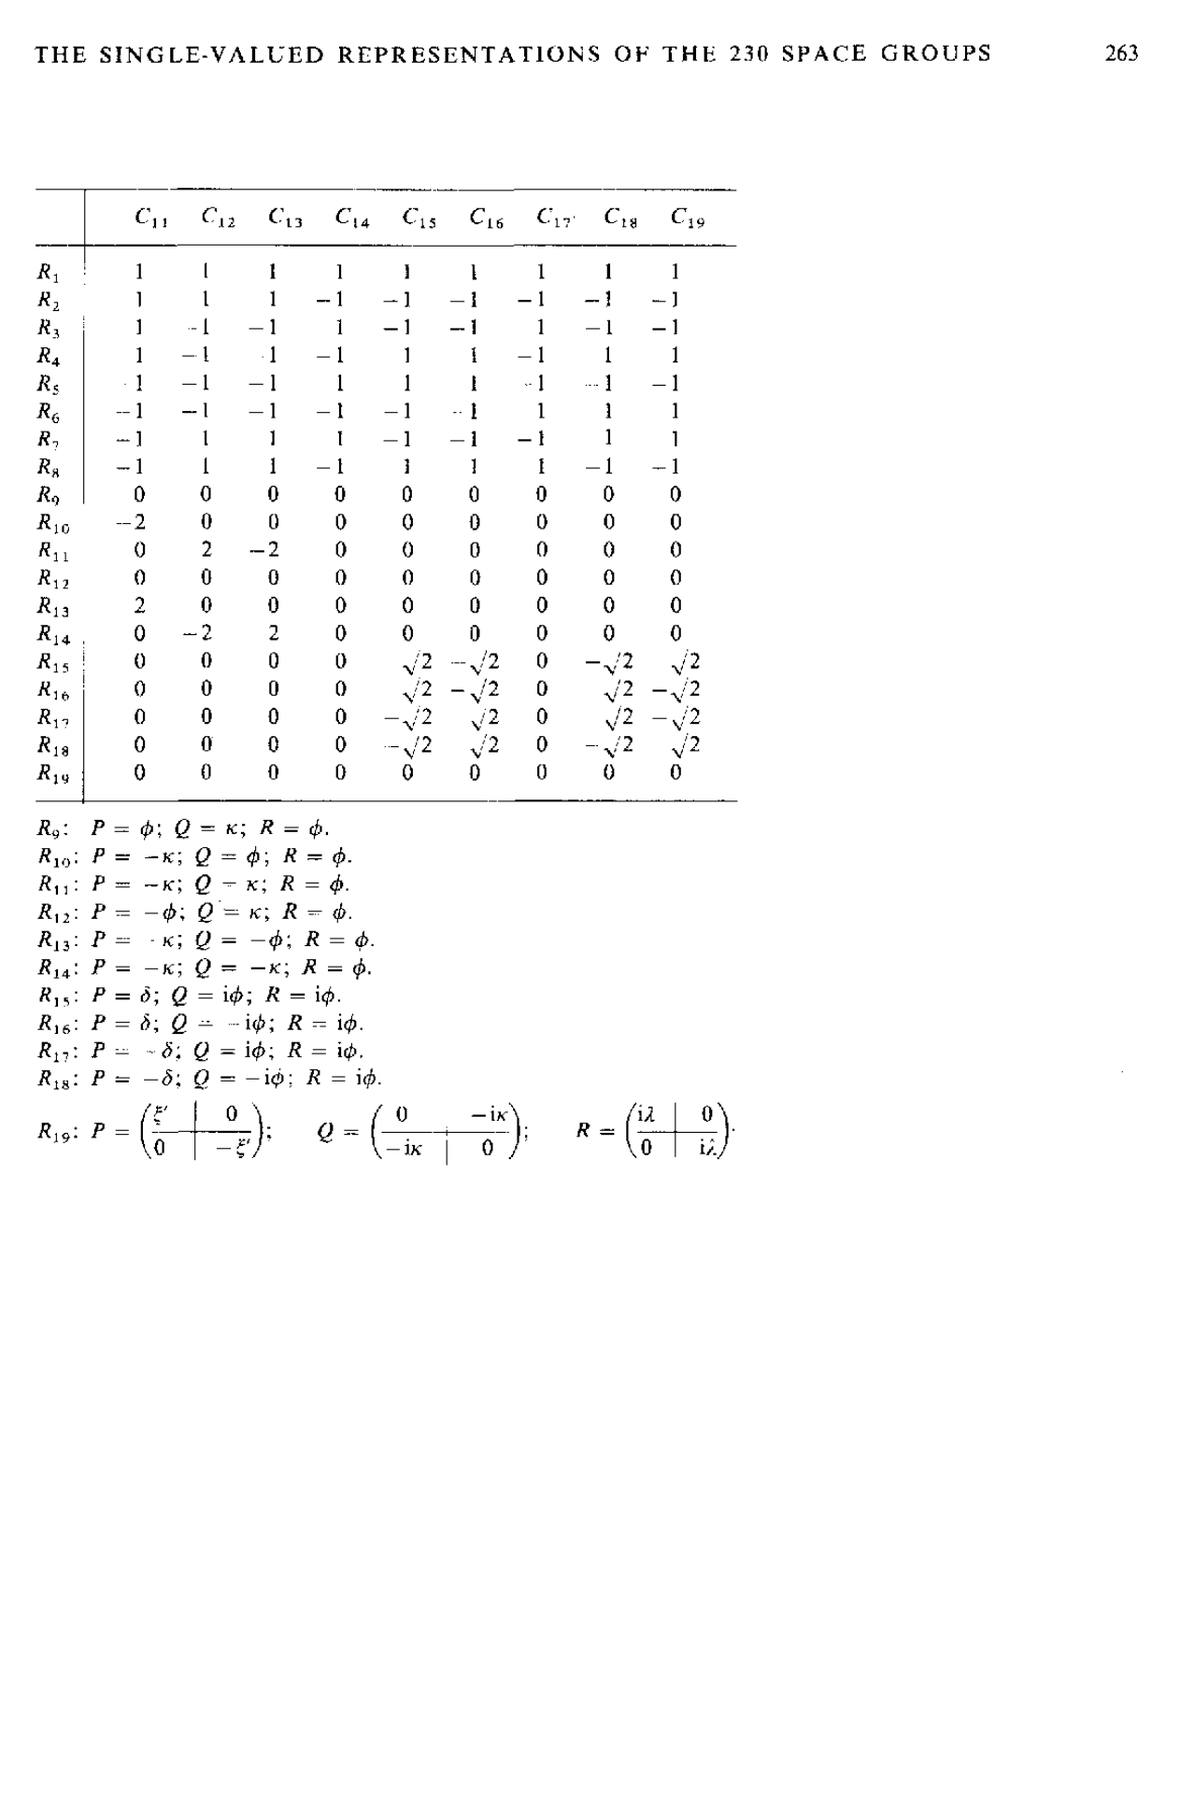
\includegraphics[width=0.86\textwidth]{c5_t51_p38.jpg}
\caption*{\textbf{表 5.1}（第 38 页，共 60 页；原书第 263 页）}
\end{figure}
\begin{figure}[H]
\centering
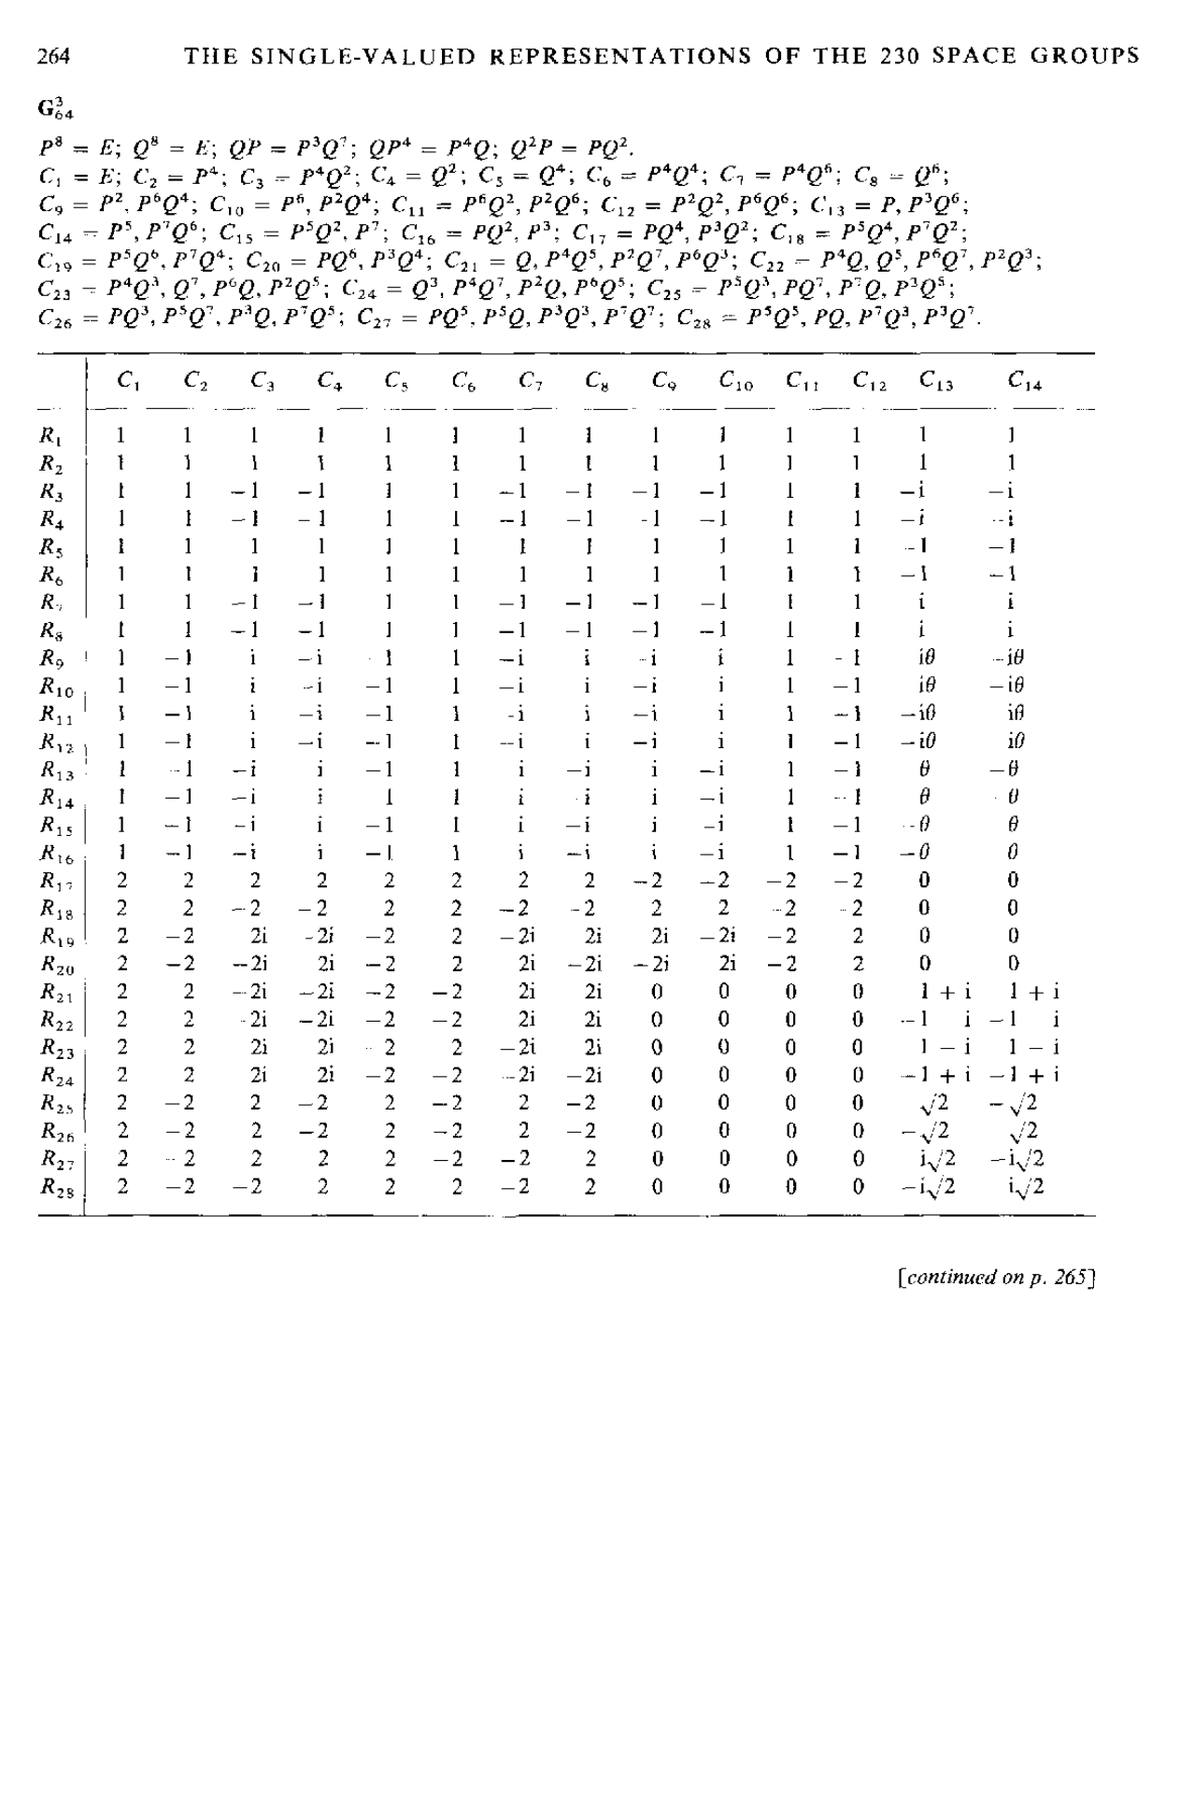
\includegraphics[width=0.86\textwidth]{c5_t51_p39.jpg}
\caption*{\textbf{表 5.1}（第 39 页，共 60 页；原书第 264 页）}
\end{figure}
\begin{figure}[H]
\centering
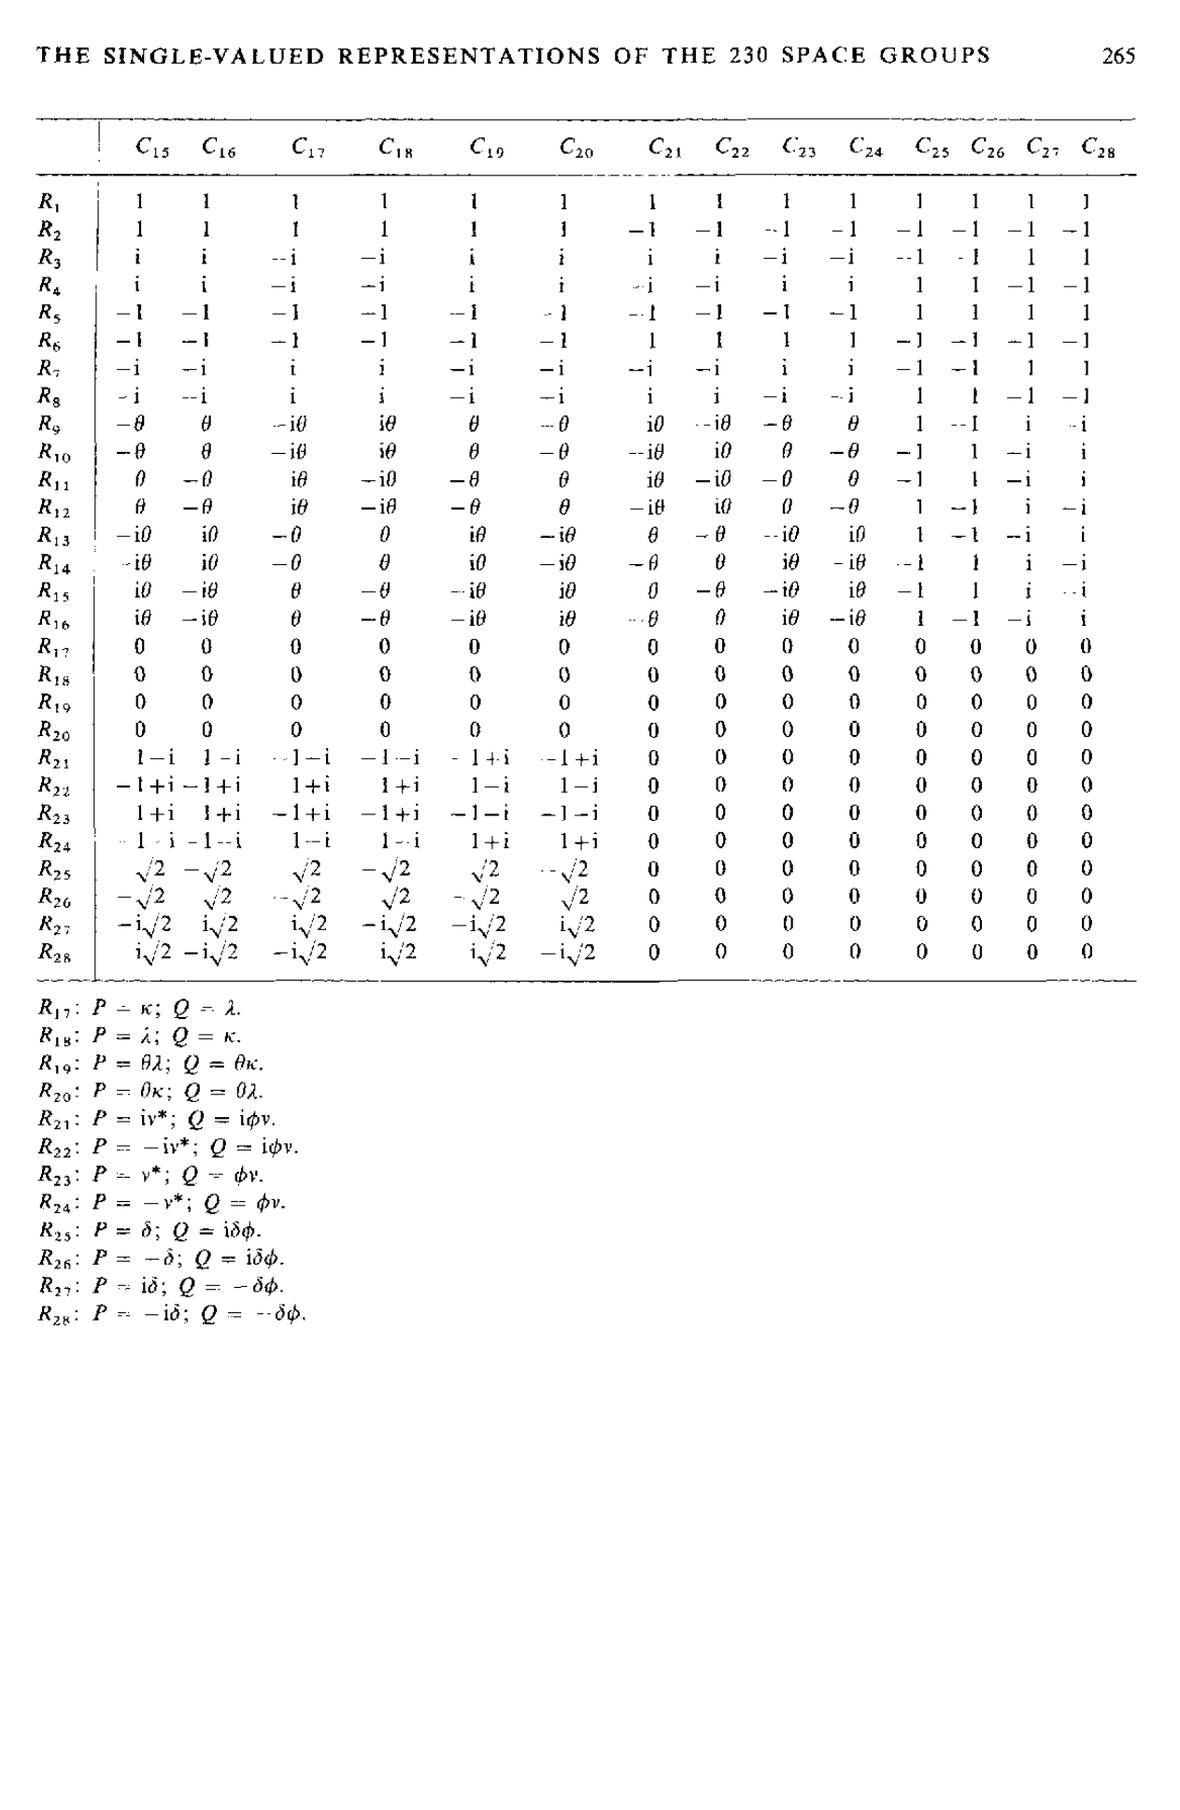
\includegraphics[width=0.86\textwidth]{c5_t51_p40.jpg}
\caption*{\textbf{表 5.1}（第 40 页，共 60 页；原书第 265 页）}
\end{figure}
\begin{figure}[H]
\centering
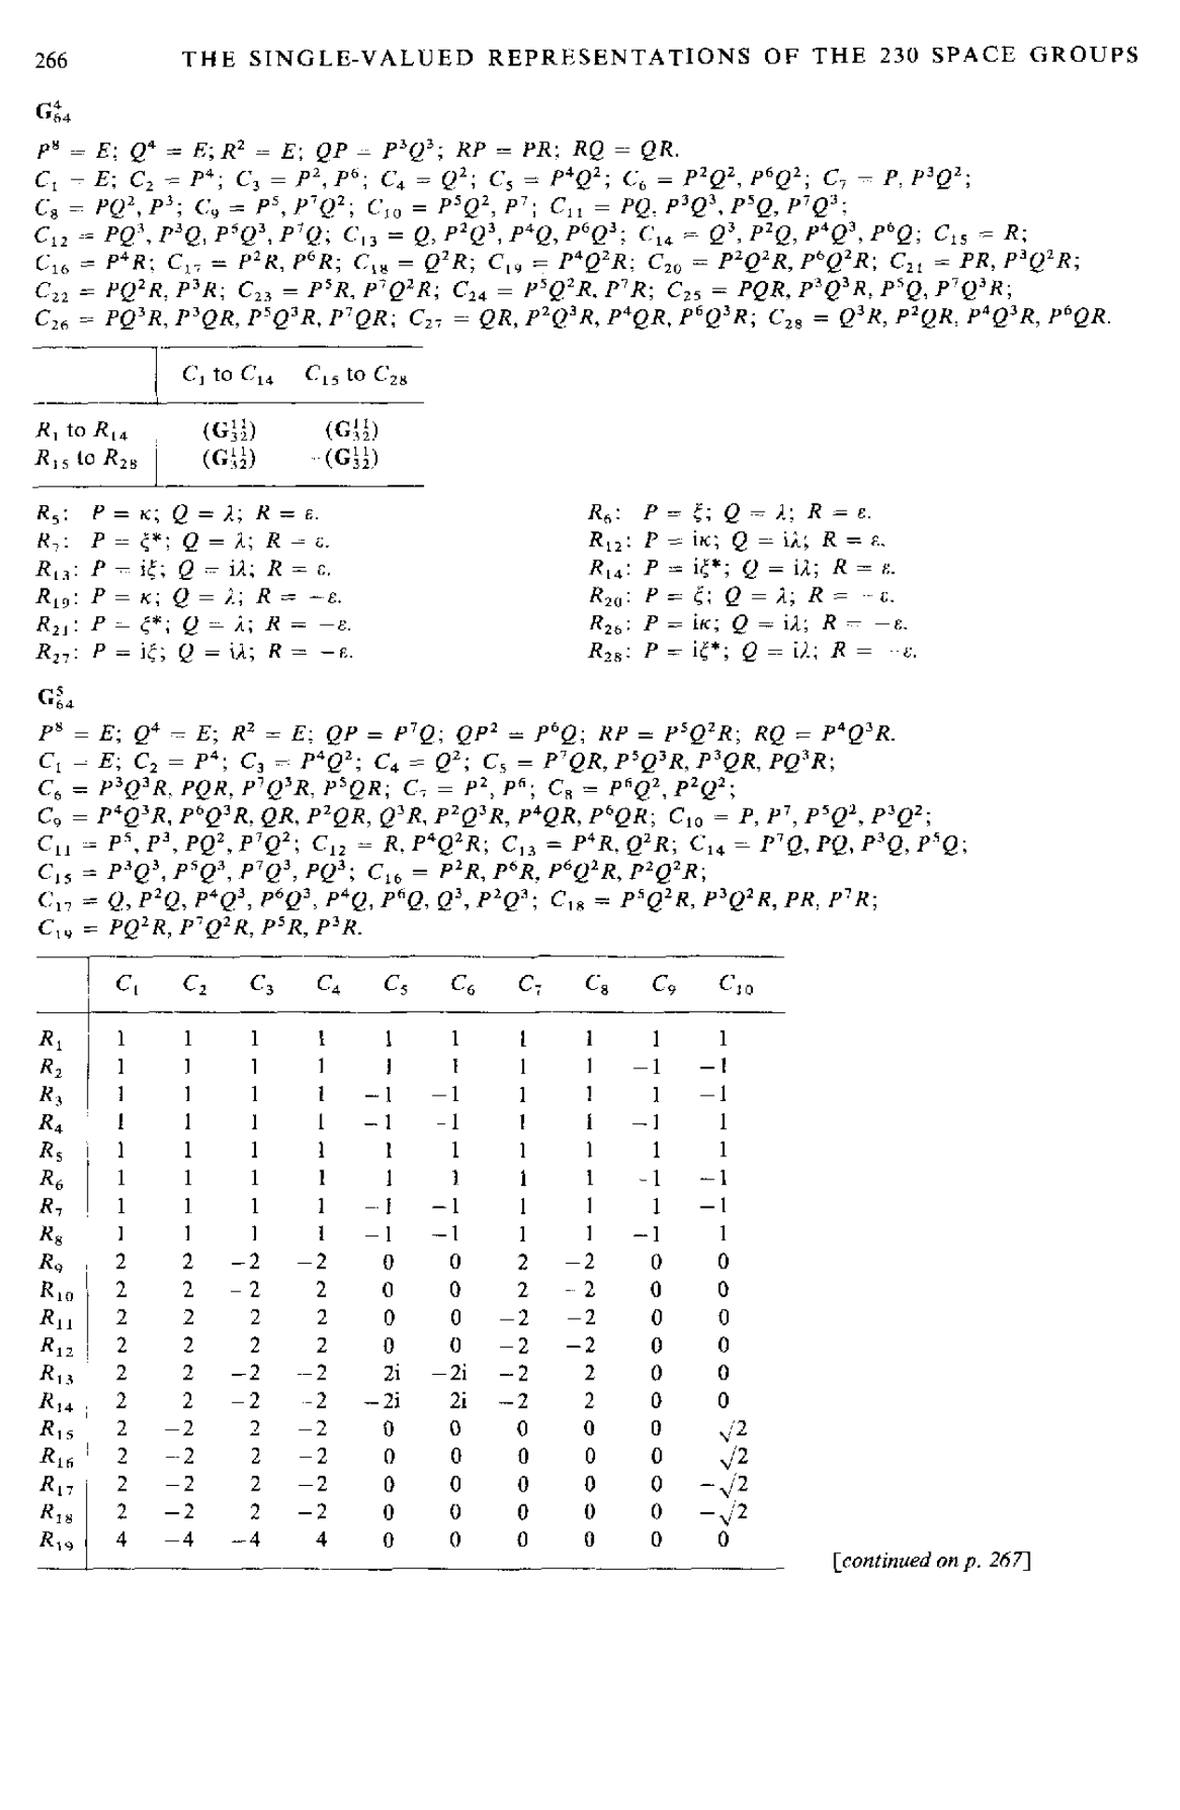
\includegraphics[width=0.86\textwidth]{c5_t51_p41.jpg}
\caption*{\textbf{表 5.1}（第 41 页，共 60 页；原书第 266 页）}
\end{figure}
\begin{figure}[H]
\centering
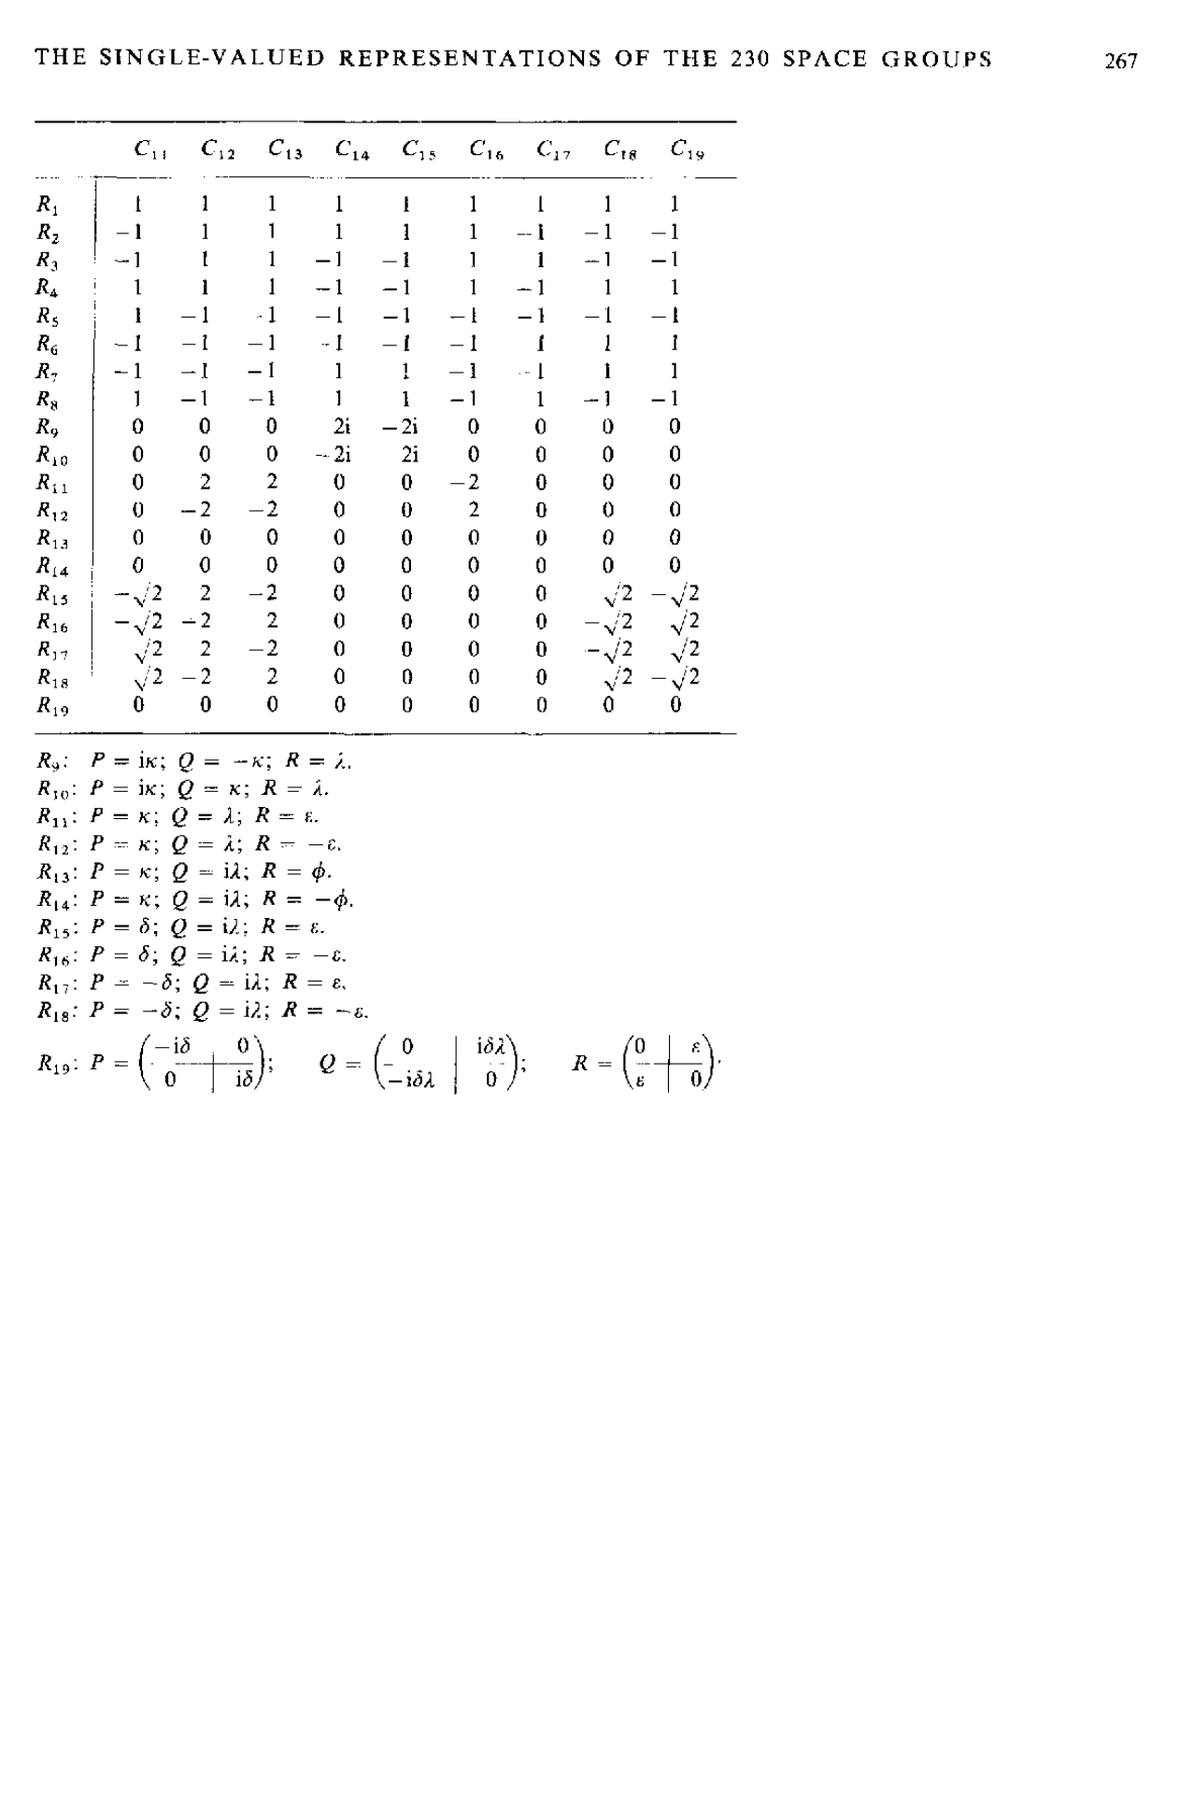
\includegraphics[width=0.86\textwidth]{c5_t51_p42.jpg}
\caption*{\textbf{表 5.1}（第 42 页，共 60 页；原书第 267 页）}
\end{figure}
\begin{figure}[H]
\centering
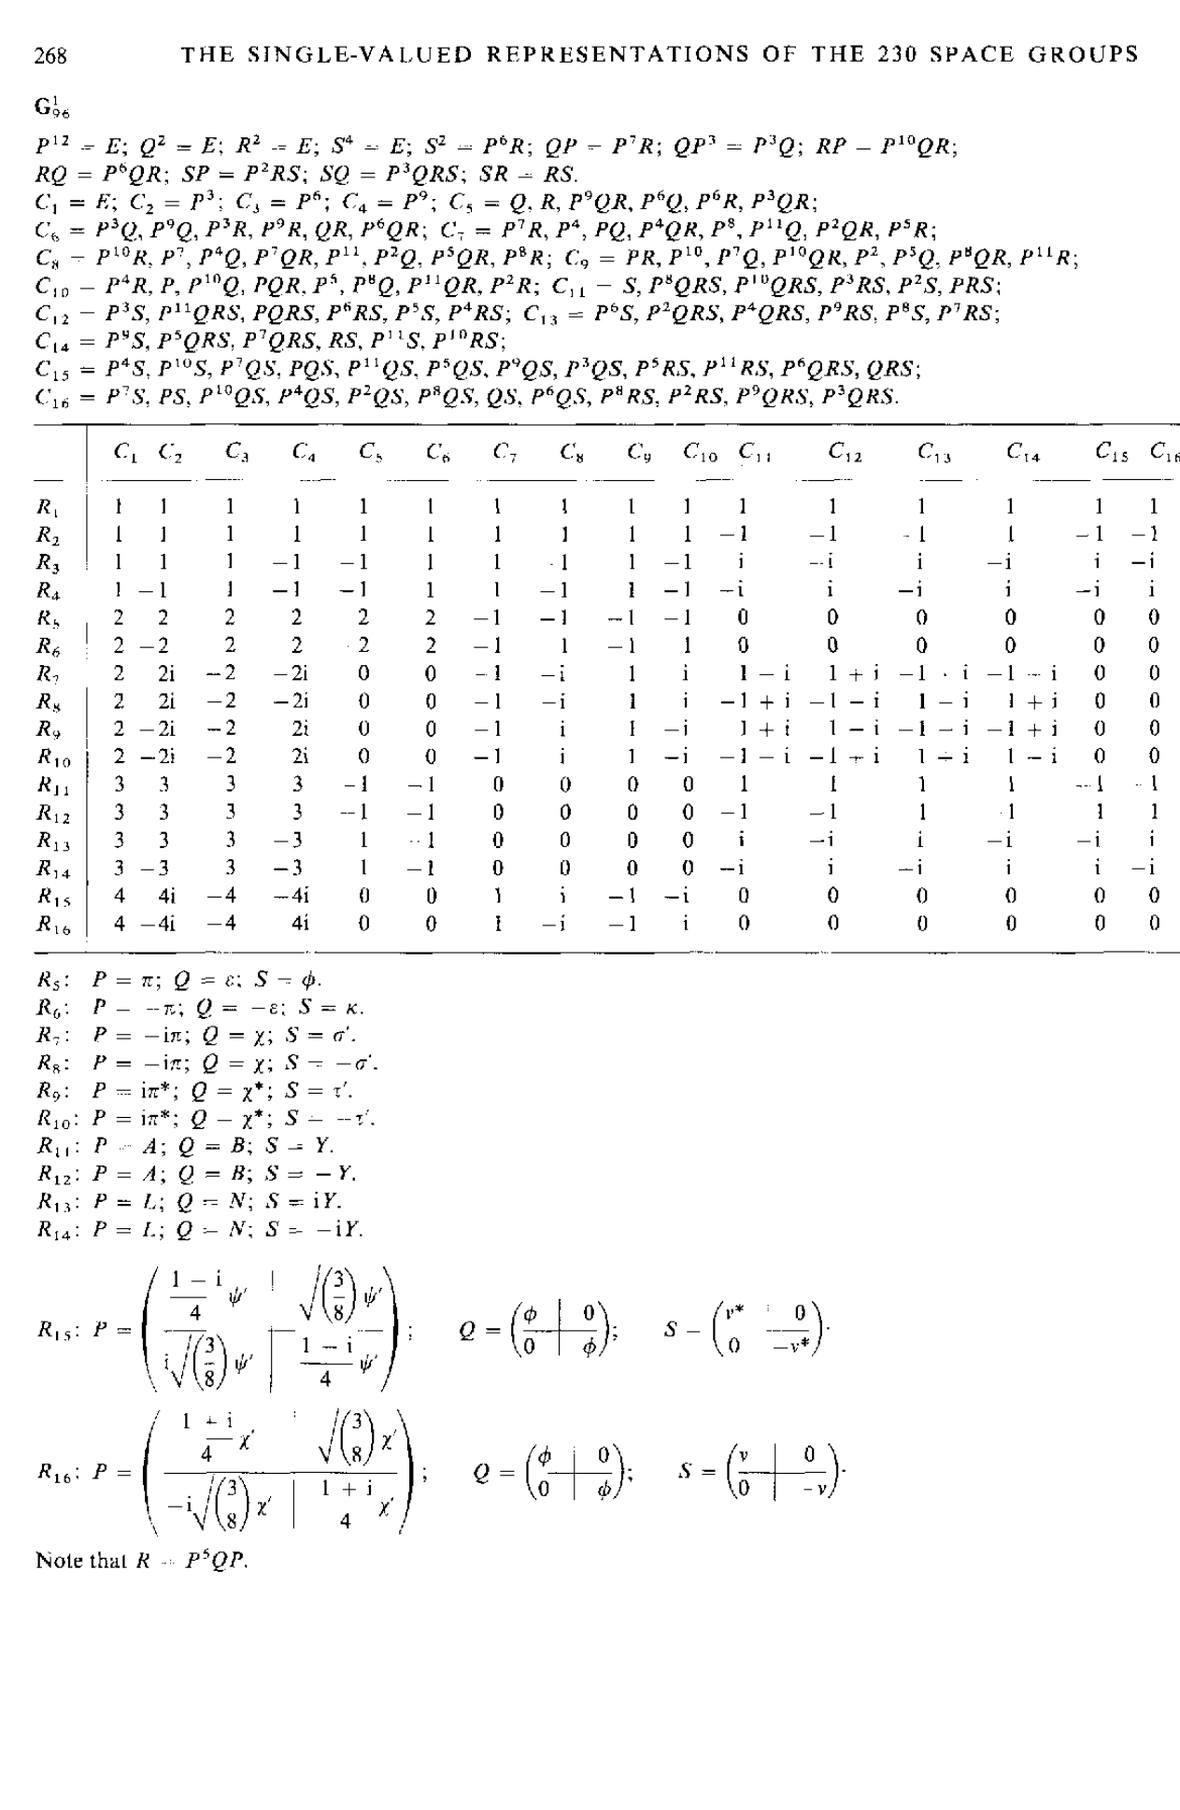
\includegraphics[width=0.86\textwidth]{c5_t51_p43.jpg}
\caption*{\textbf{表 5.1}（第 43 页，共 60 页；原书第 268 页）}
\end{figure}
\begin{figure}[H]
\centering
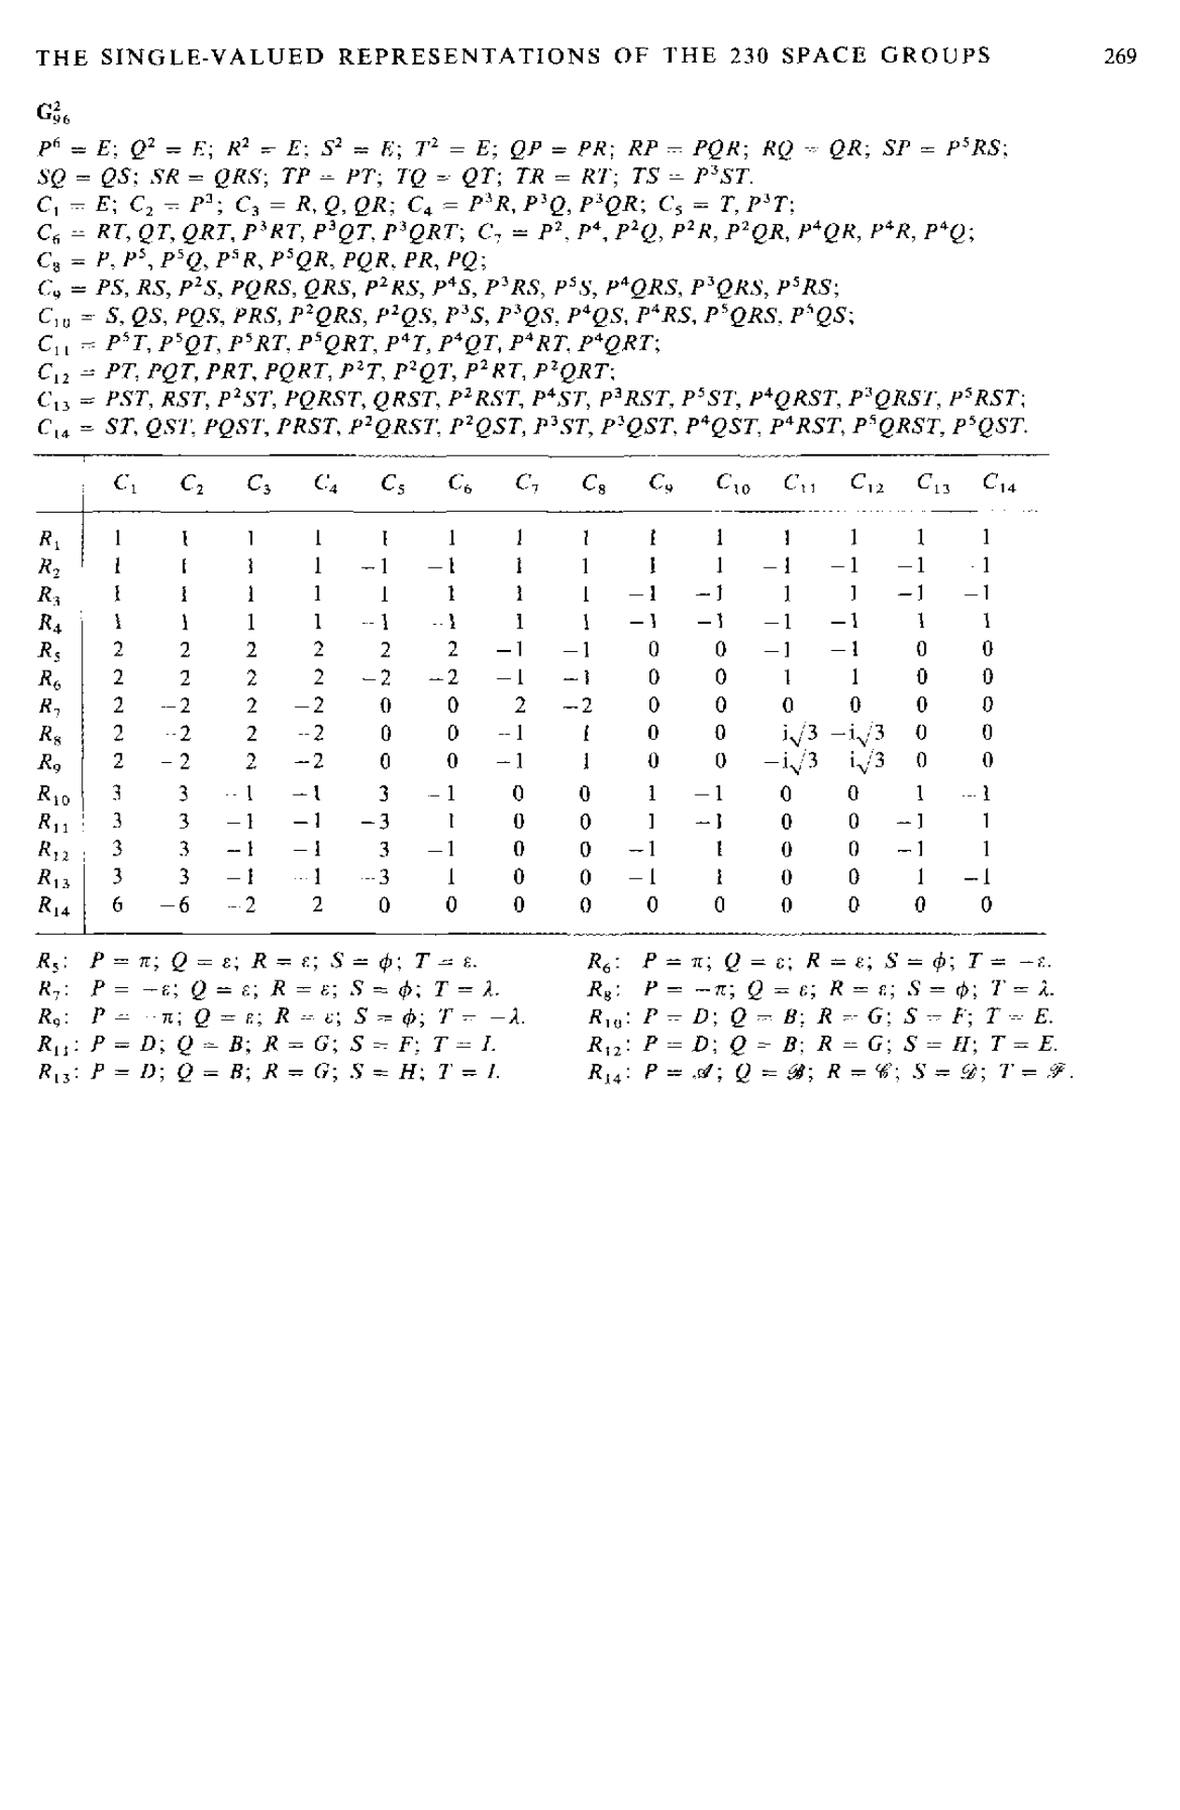
\includegraphics[width=0.86\textwidth]{c5_t51_p44.jpg}
\caption*{\textbf{表 5.1}（第 44 页，共 60 页；原书第 269 页）}
\end{figure}
\begin{figure}[H]
\centering
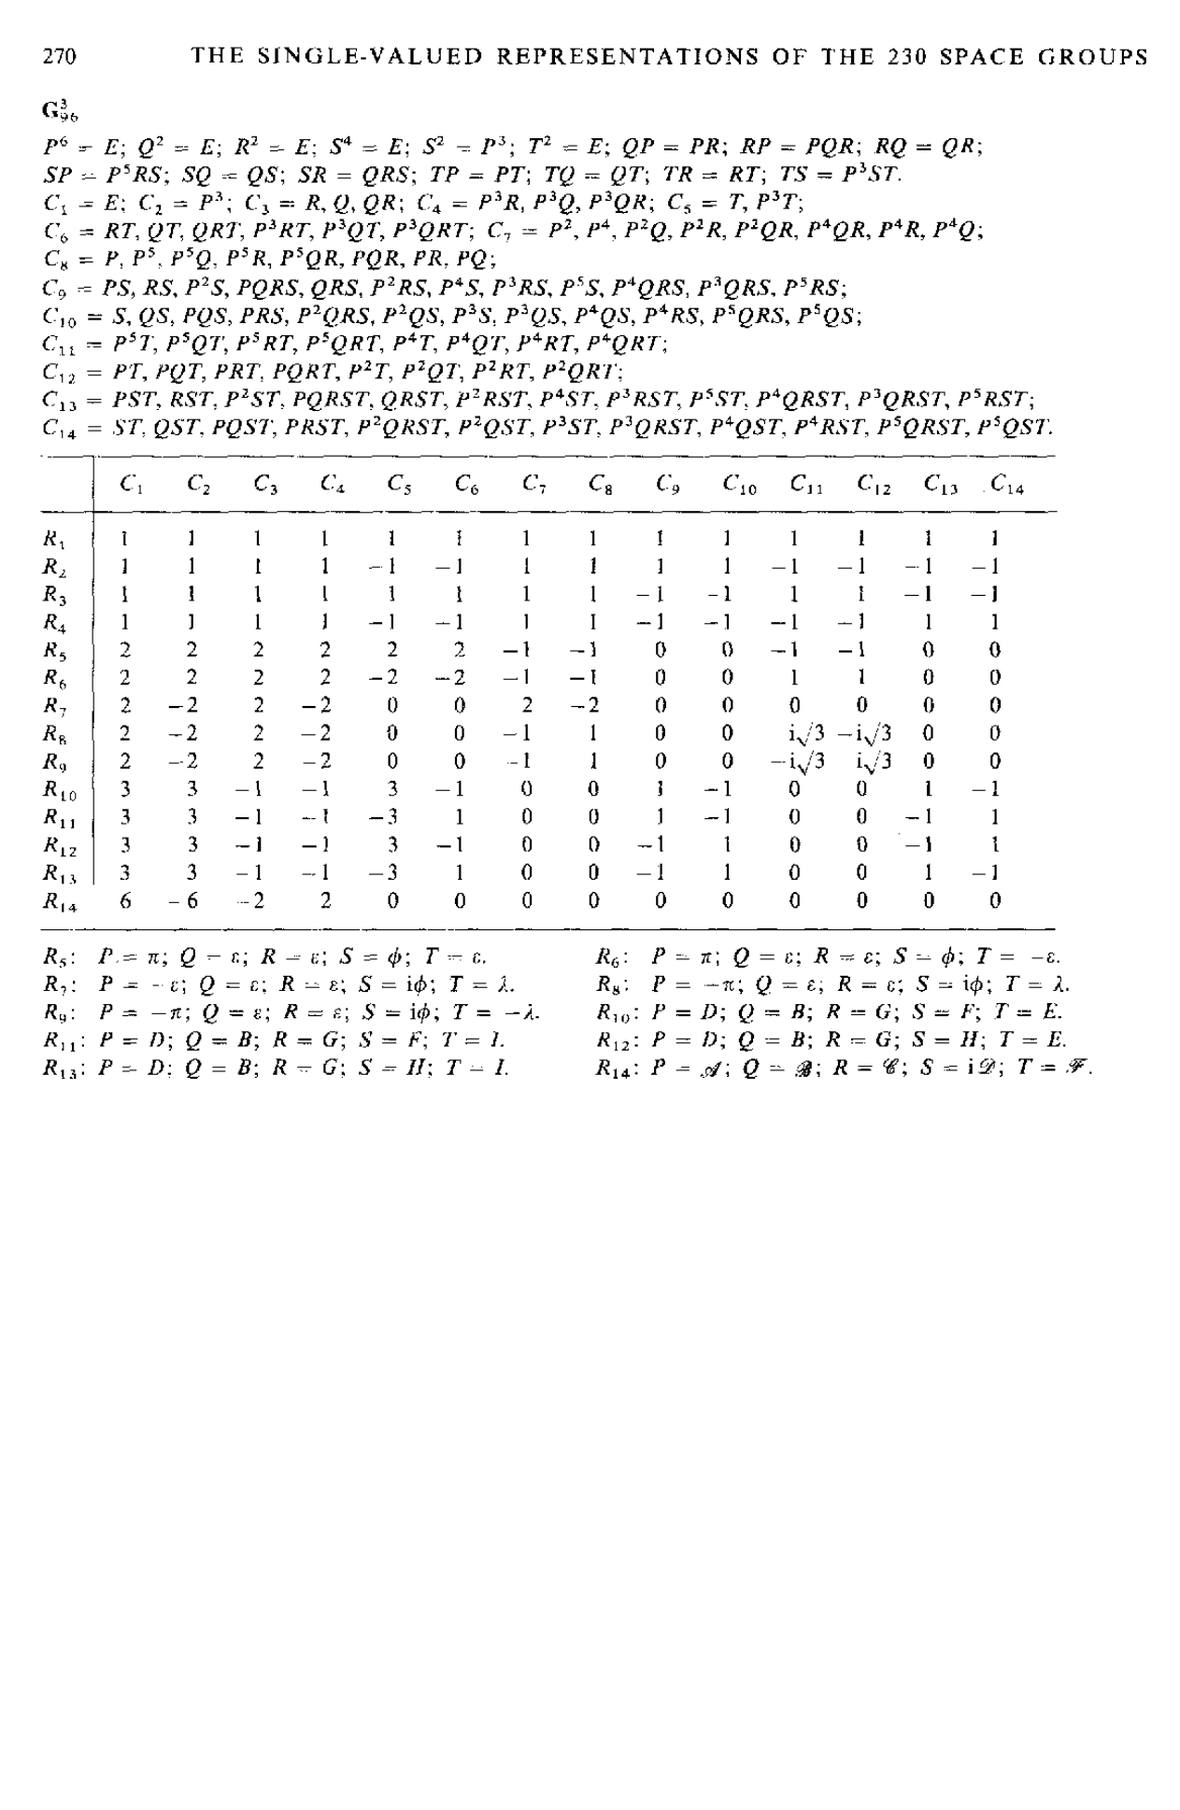
\includegraphics[width=0.86\textwidth]{c5_t51_p45.jpg}
\caption*{\textbf{表 5.1}（第 45 页，共 60 页；原书第 270 页）}
\end{figure}
\begin{figure}[H]
\centering
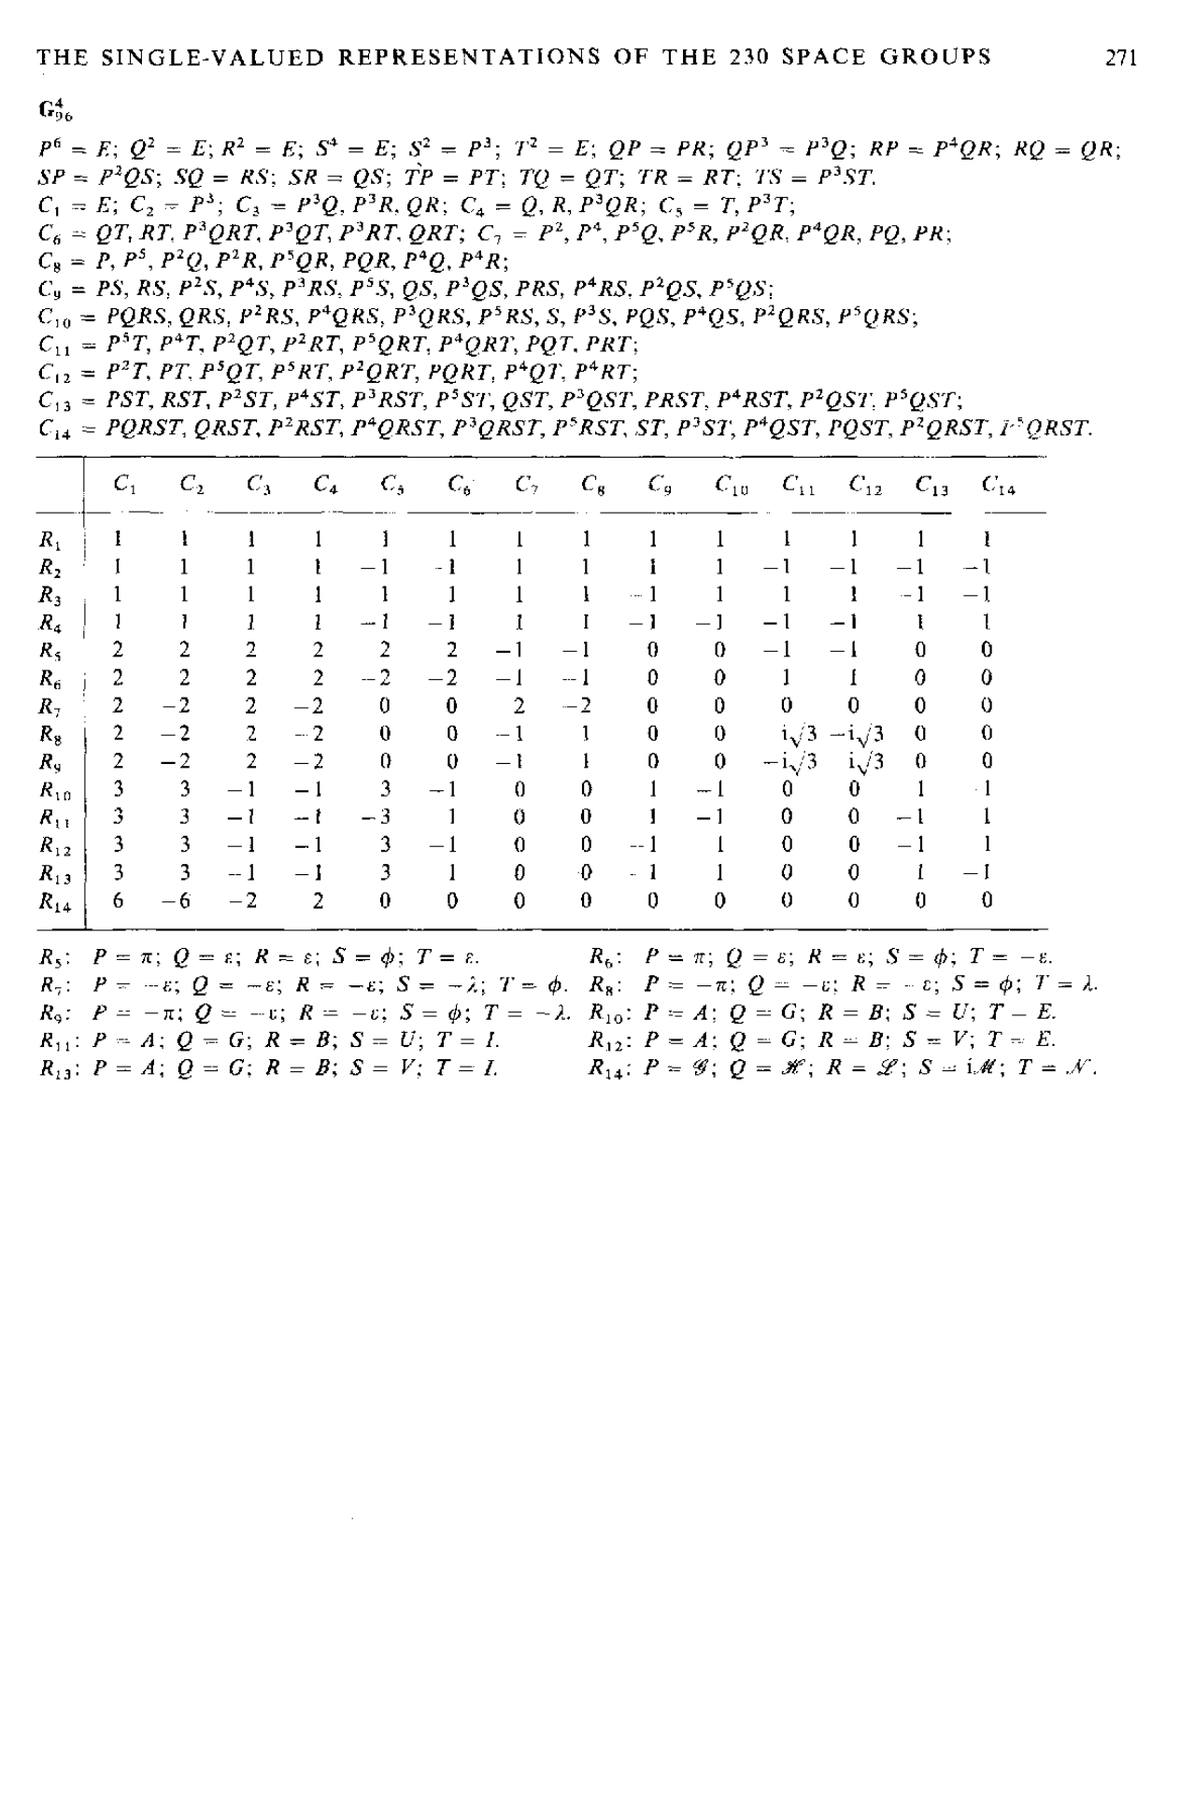
\includegraphics[width=0.86\textwidth]{c5_t51_p46.jpg}
\caption*{\textbf{表 5.1}（第 46 页，共 60 页；原书第 271 页）}
\end{figure}
\begin{figure}[H]
\centering
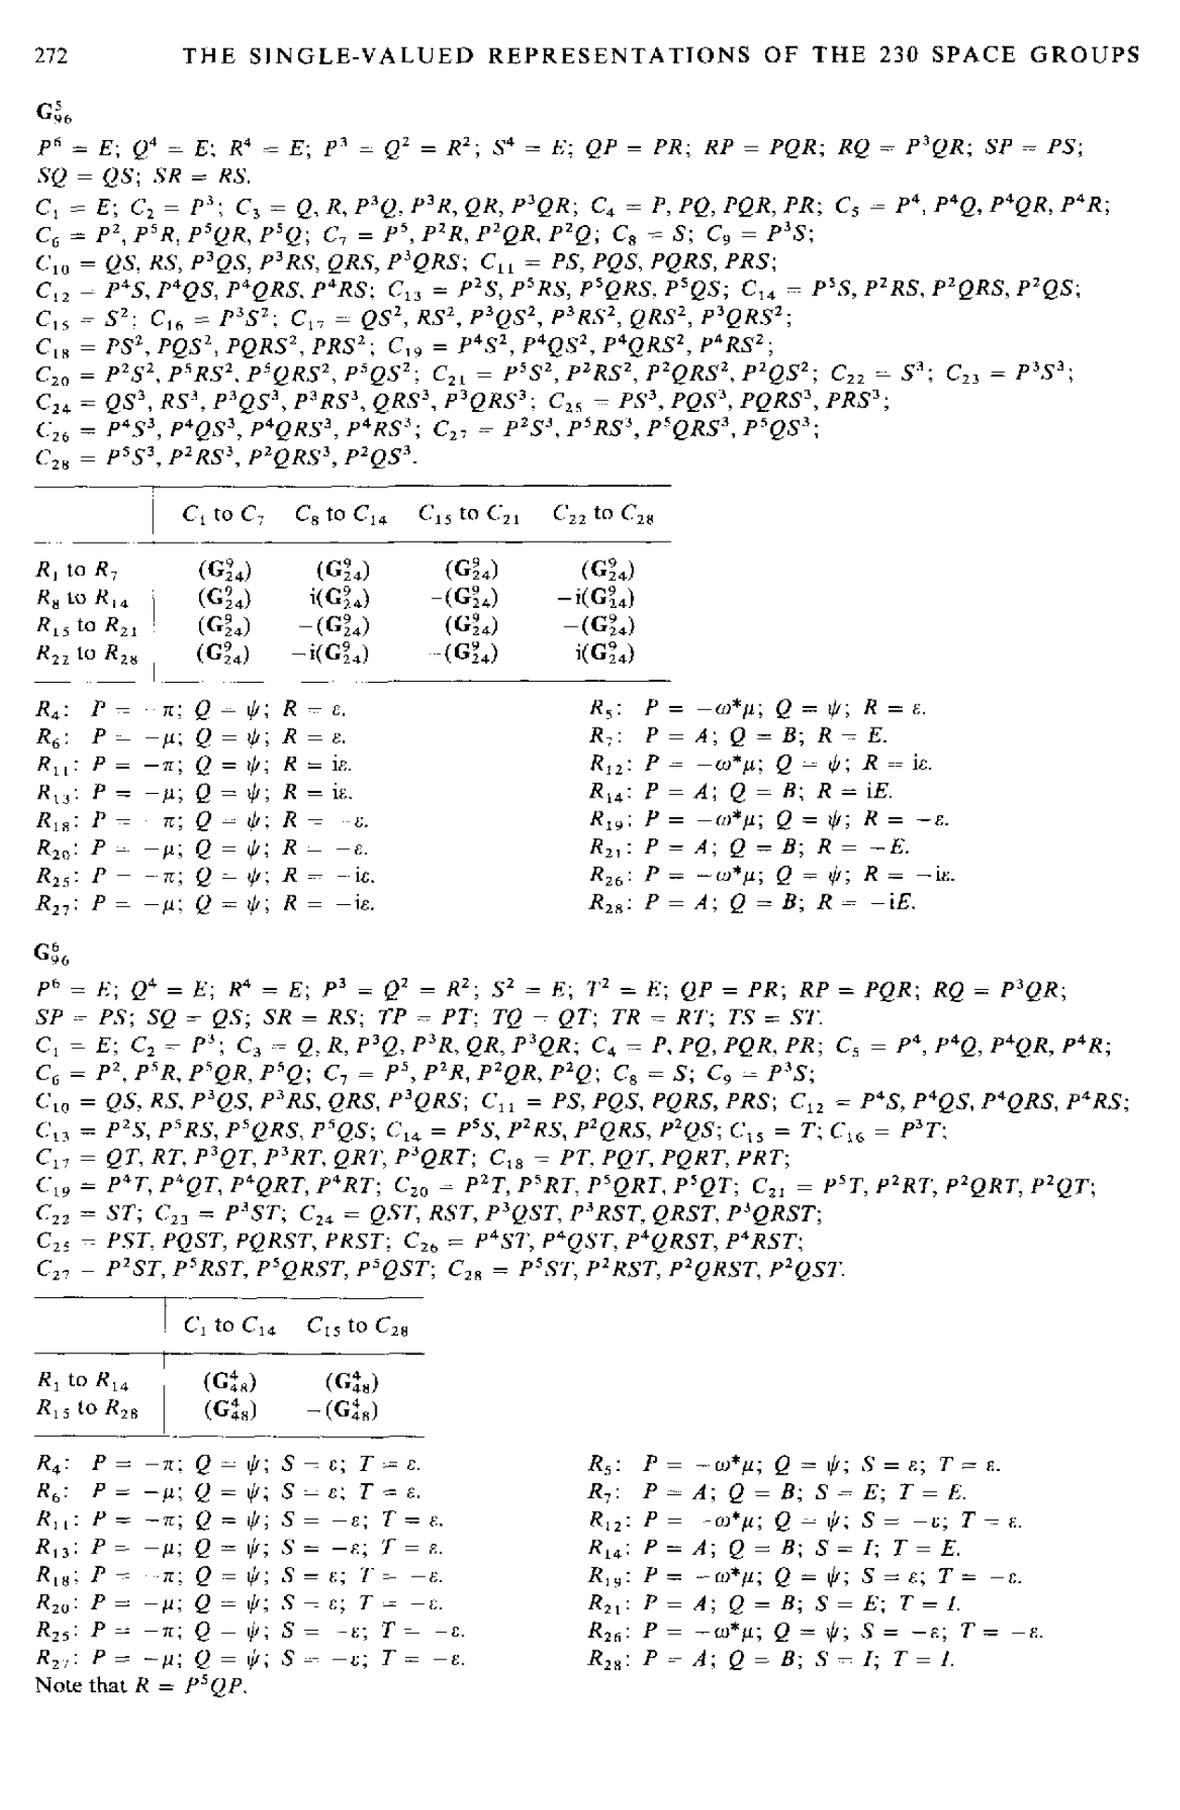
\includegraphics[width=0.86\textwidth]{c5_t51_p47.jpg}
\caption*{\textbf{表 5.1}（第 47 页，共 60 页；原书第 272 页）}
\end{figure}
\begin{figure}[H]
\centering
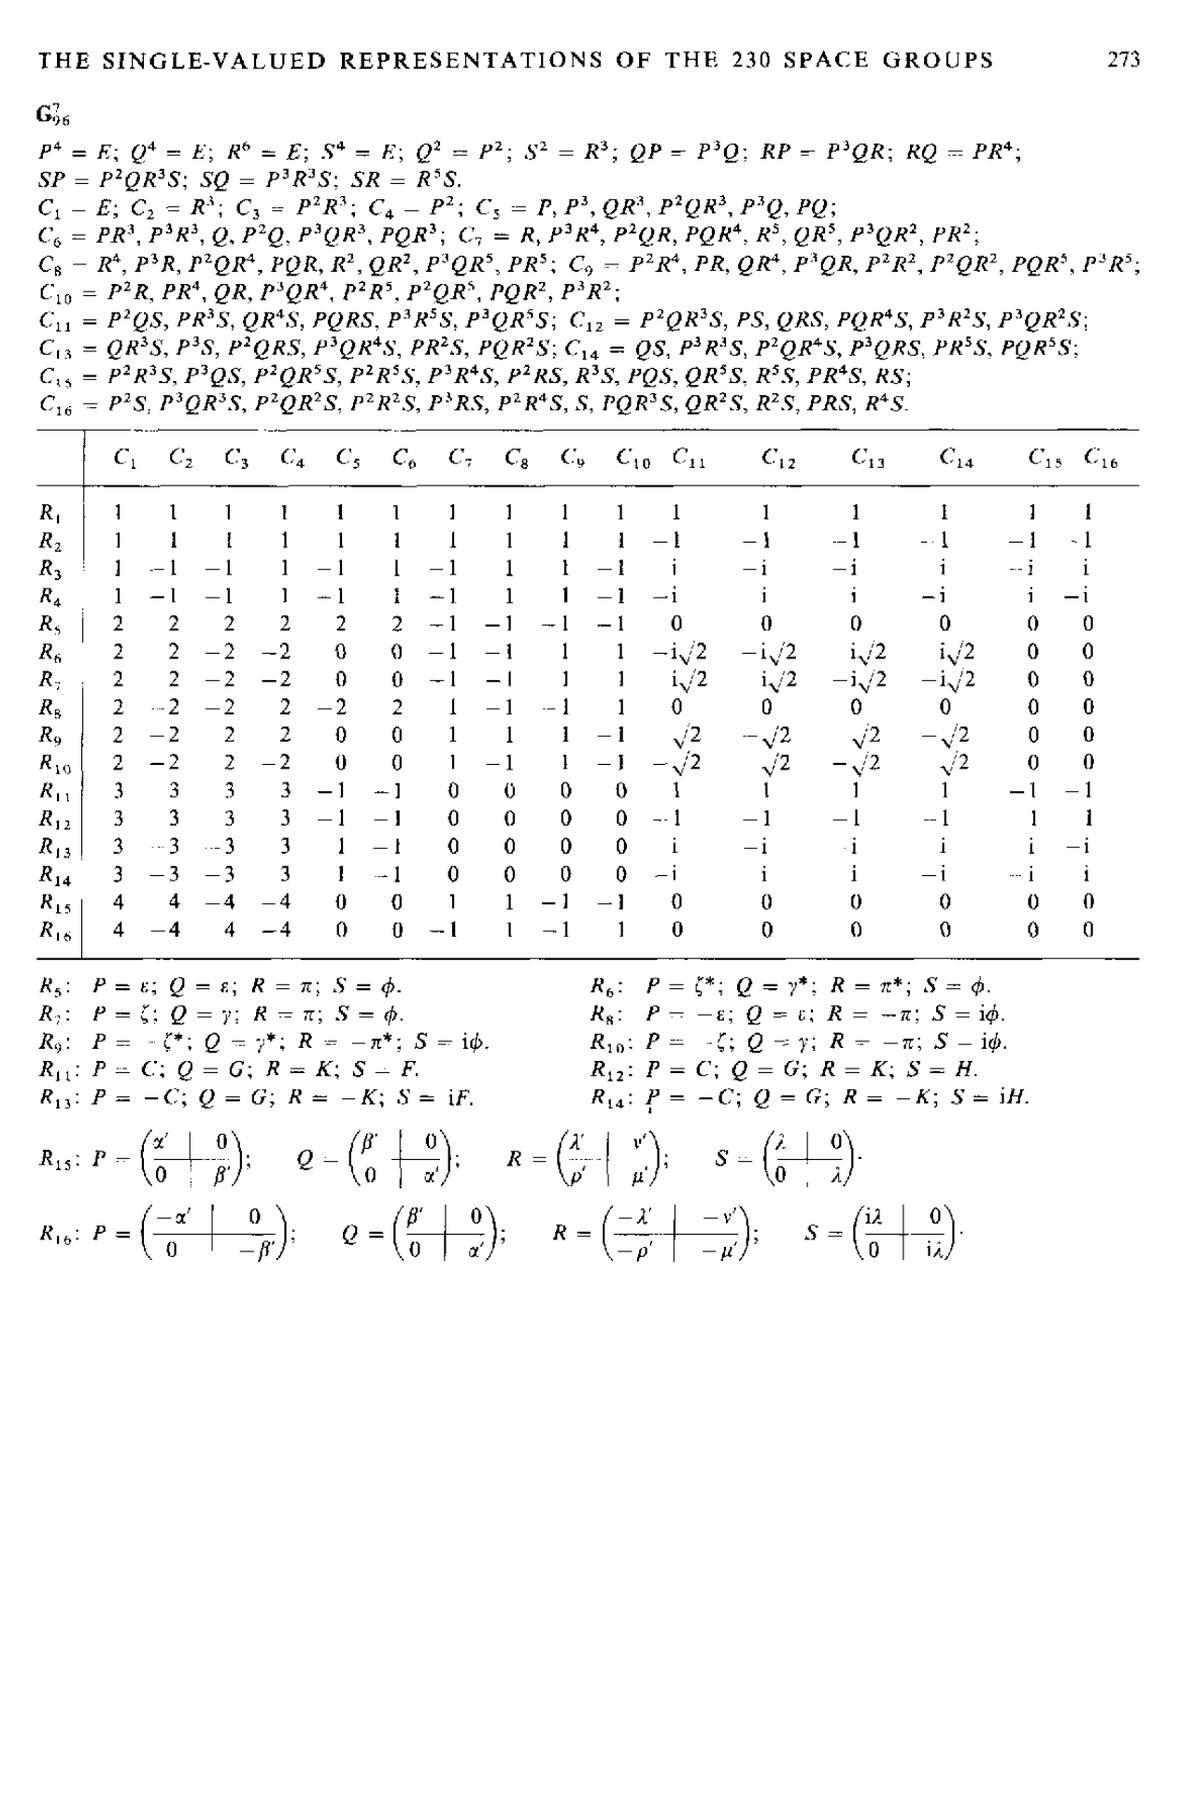
\includegraphics[width=0.86\textwidth]{c5_t51_p48.jpg}
\caption*{\textbf{表 5.1}（第 48 页，共 60 页；原书第 273 页）}
\end{figure}
\begin{figure}[H]
\centering
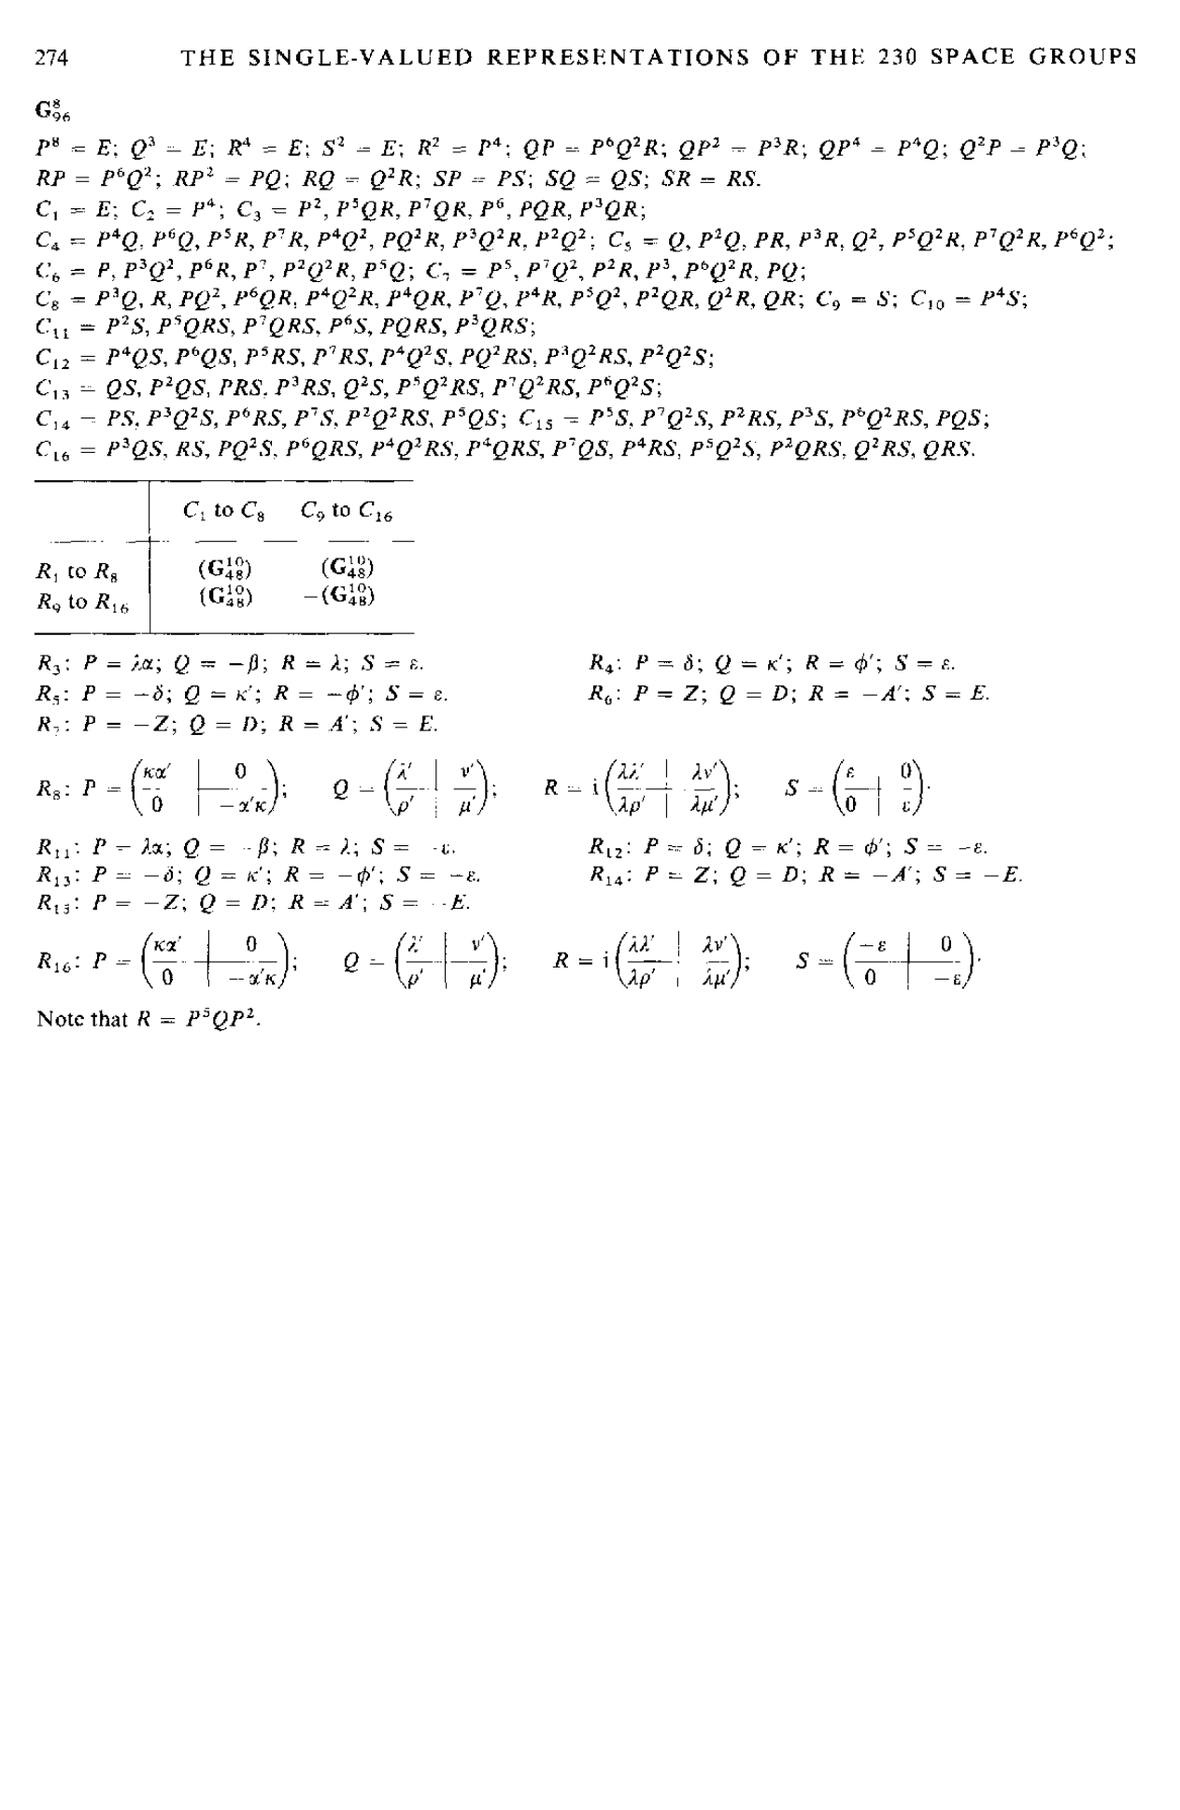
\includegraphics[width=0.86\textwidth]{c5_t51_p49.jpg}
\caption*{\textbf{表 5.1}（第 49 页，共 60 页；原书第 274 页）}
\end{figure}
\begin{figure}[H]
\centering
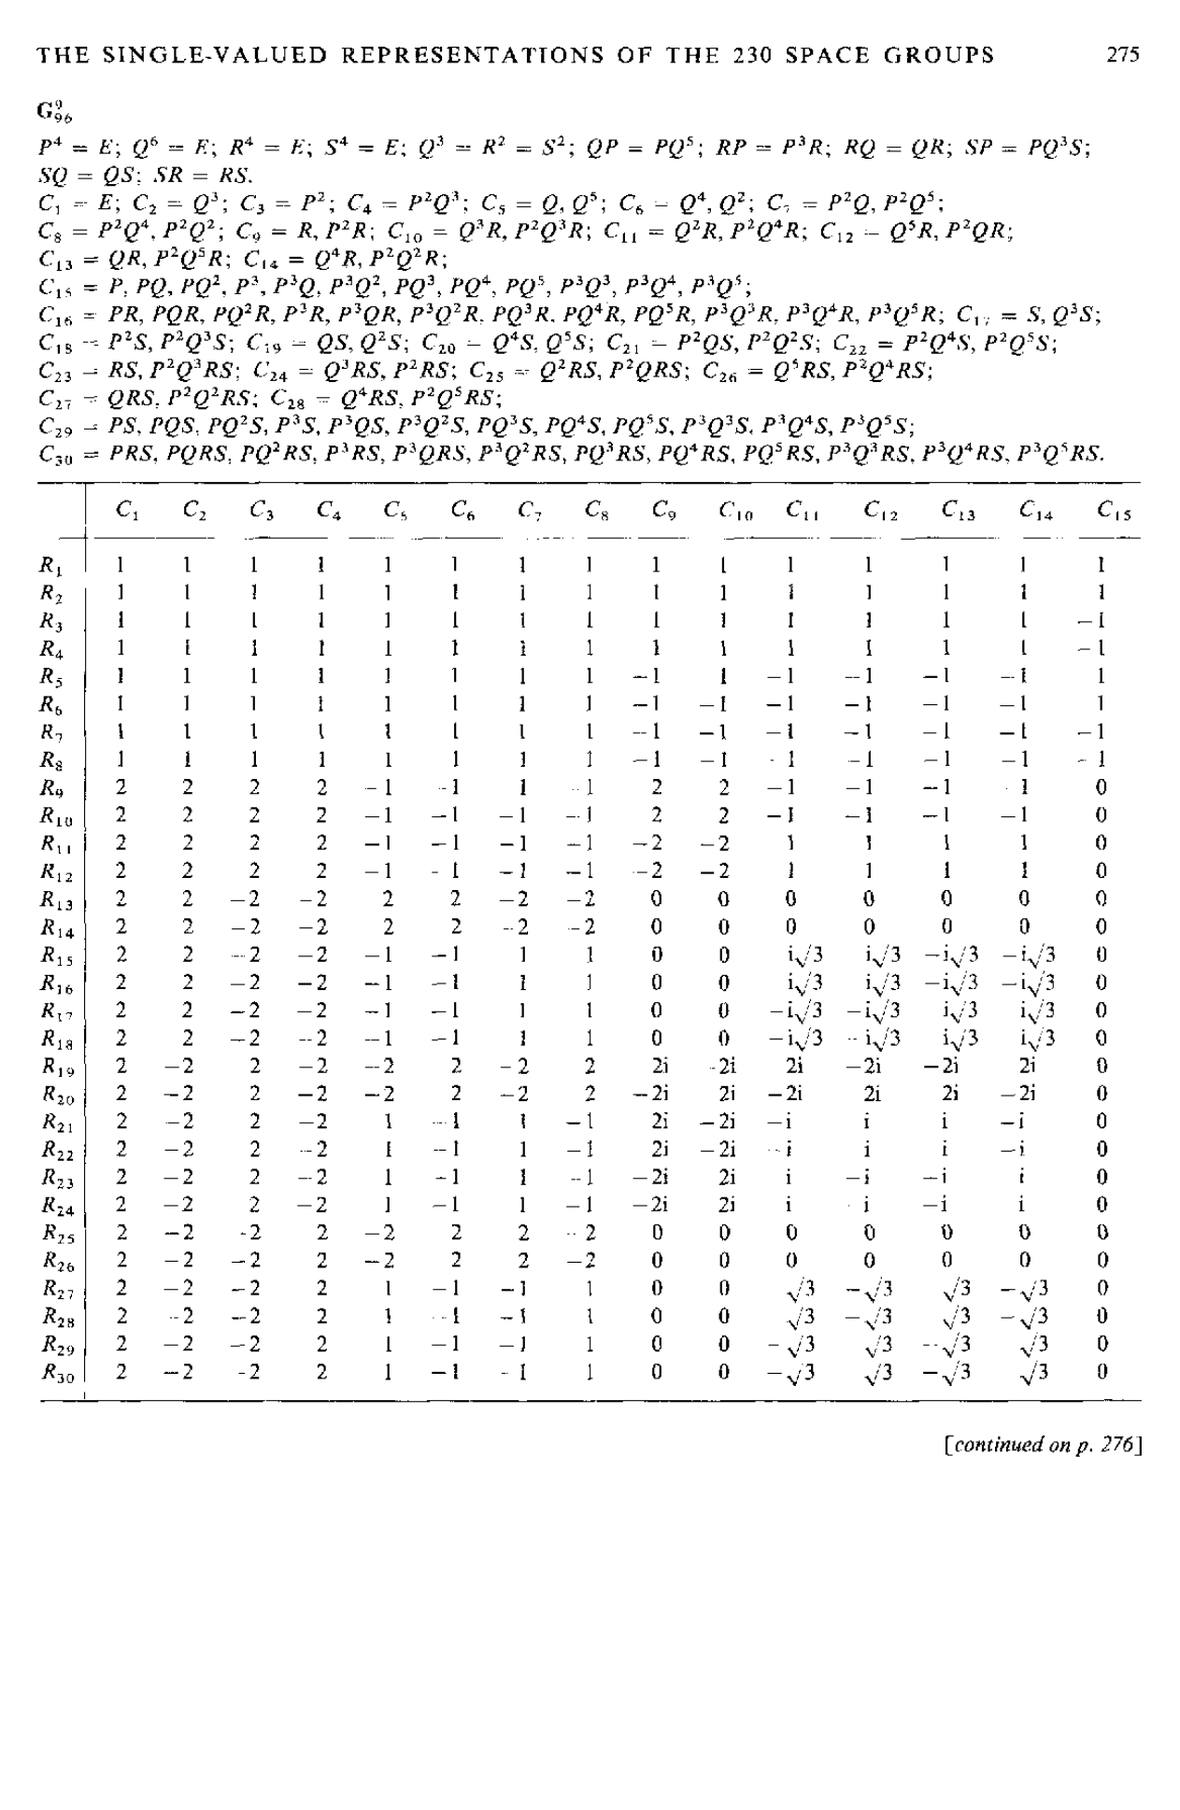
\includegraphics[width=0.86\textwidth]{c5_t51_p50.jpg}
\caption*{\textbf{表 5.1}（第 50 页，共 60 页；原书第 275 页）}
\end{figure}
\begin{figure}[H]
\centering
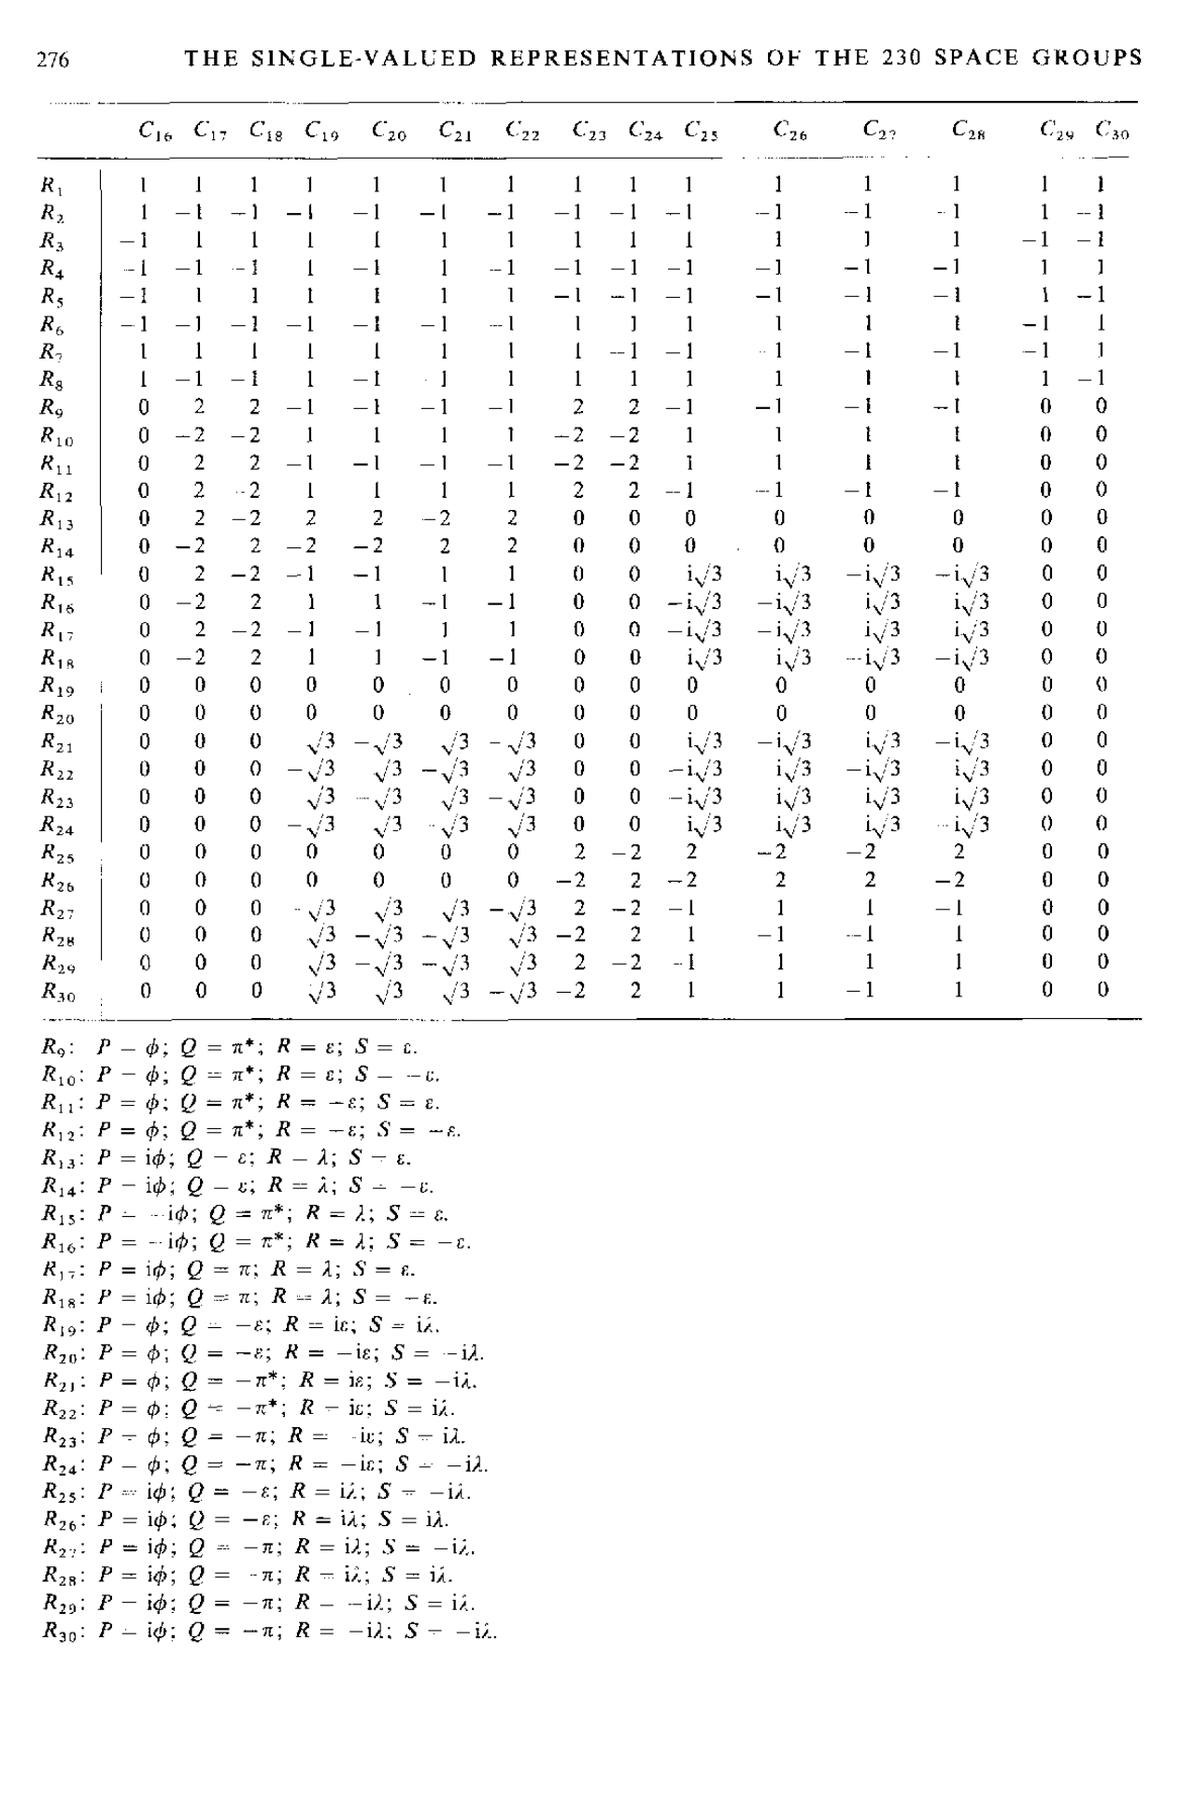
\includegraphics[width=0.86\textwidth]{c5_t51_p51.jpg}
\caption*{\textbf{表 5.1}（第 51 页，共 60 页；原书第 276 页）}
\end{figure}
\begin{figure}[H]
\centering
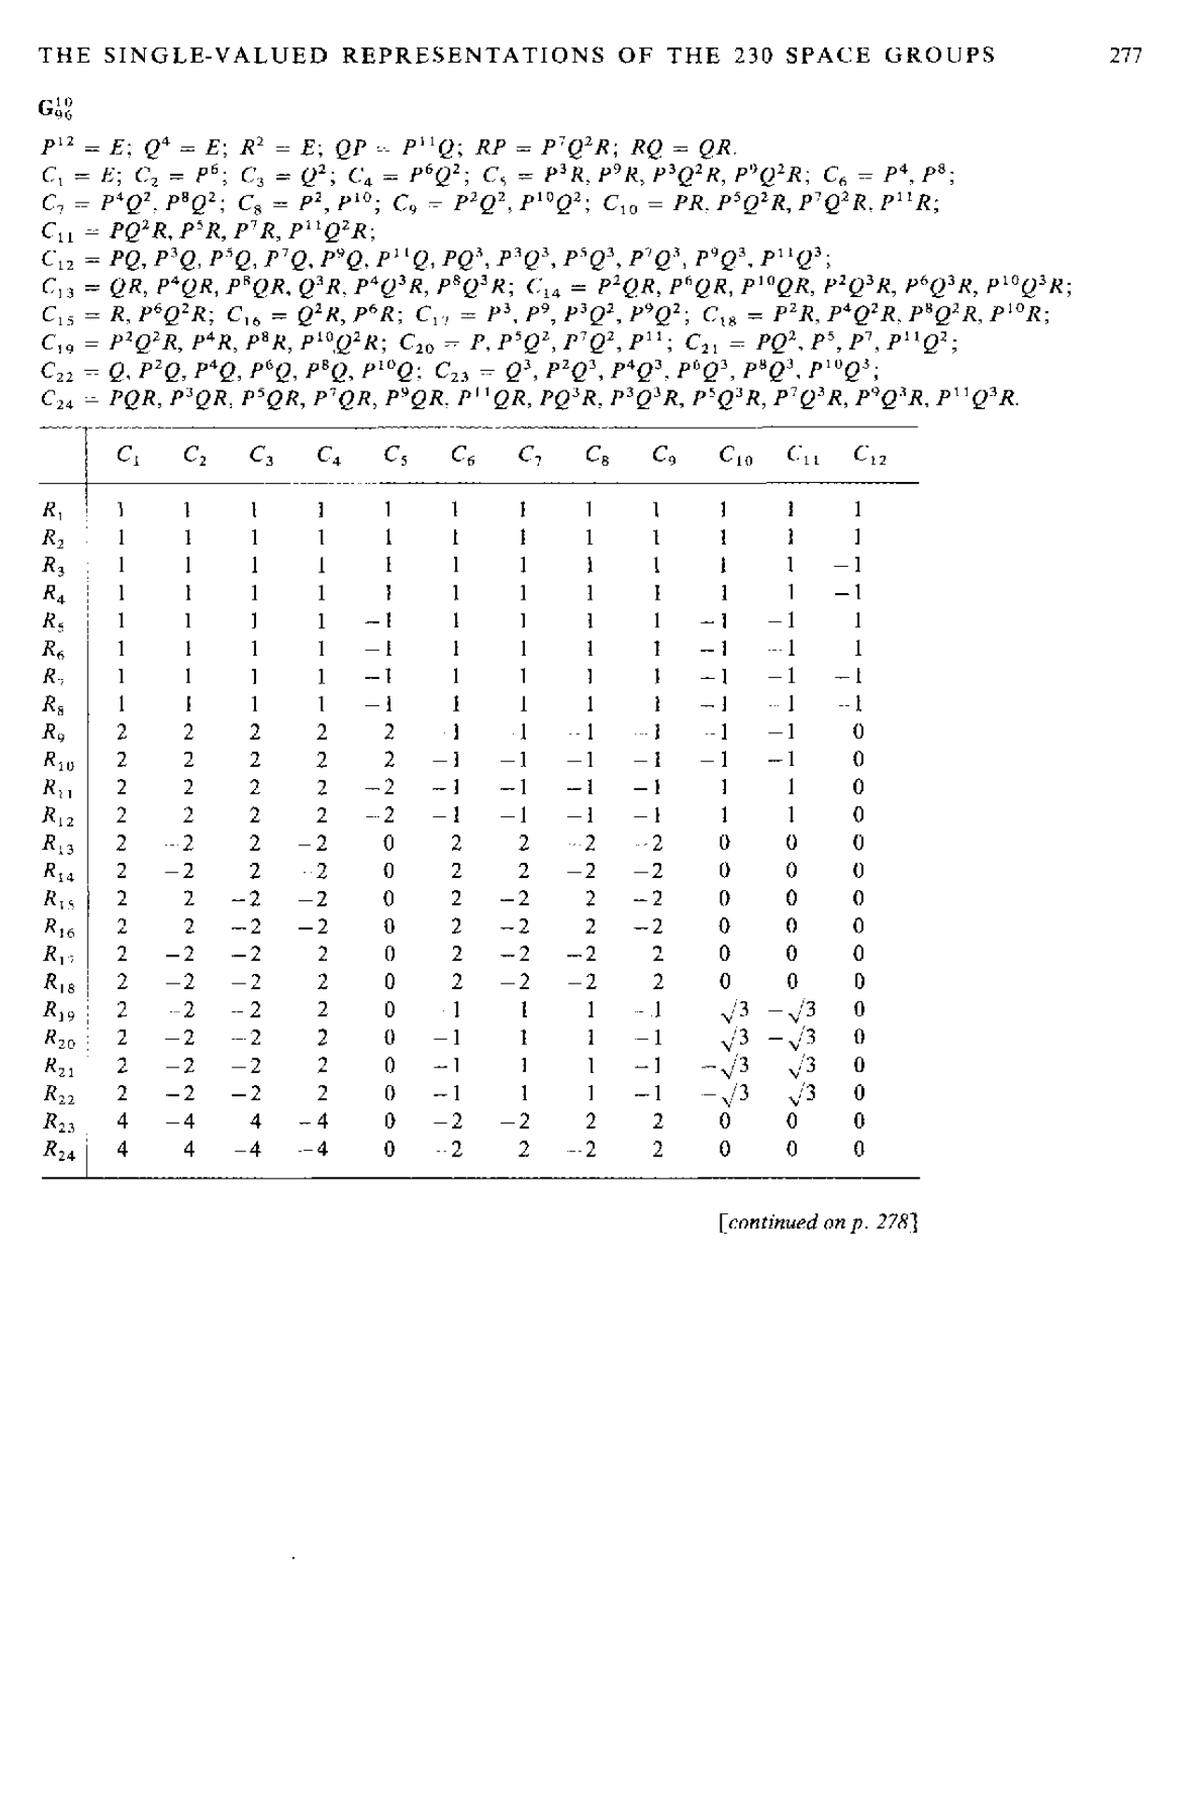
\includegraphics[width=0.86\textwidth]{c5_t51_p52.jpg}
\caption*{\textbf{表 5.1}（第 52 页，共 60 页；原书第 277 页）}
\end{figure}
\begin{figure}[H]
\centering
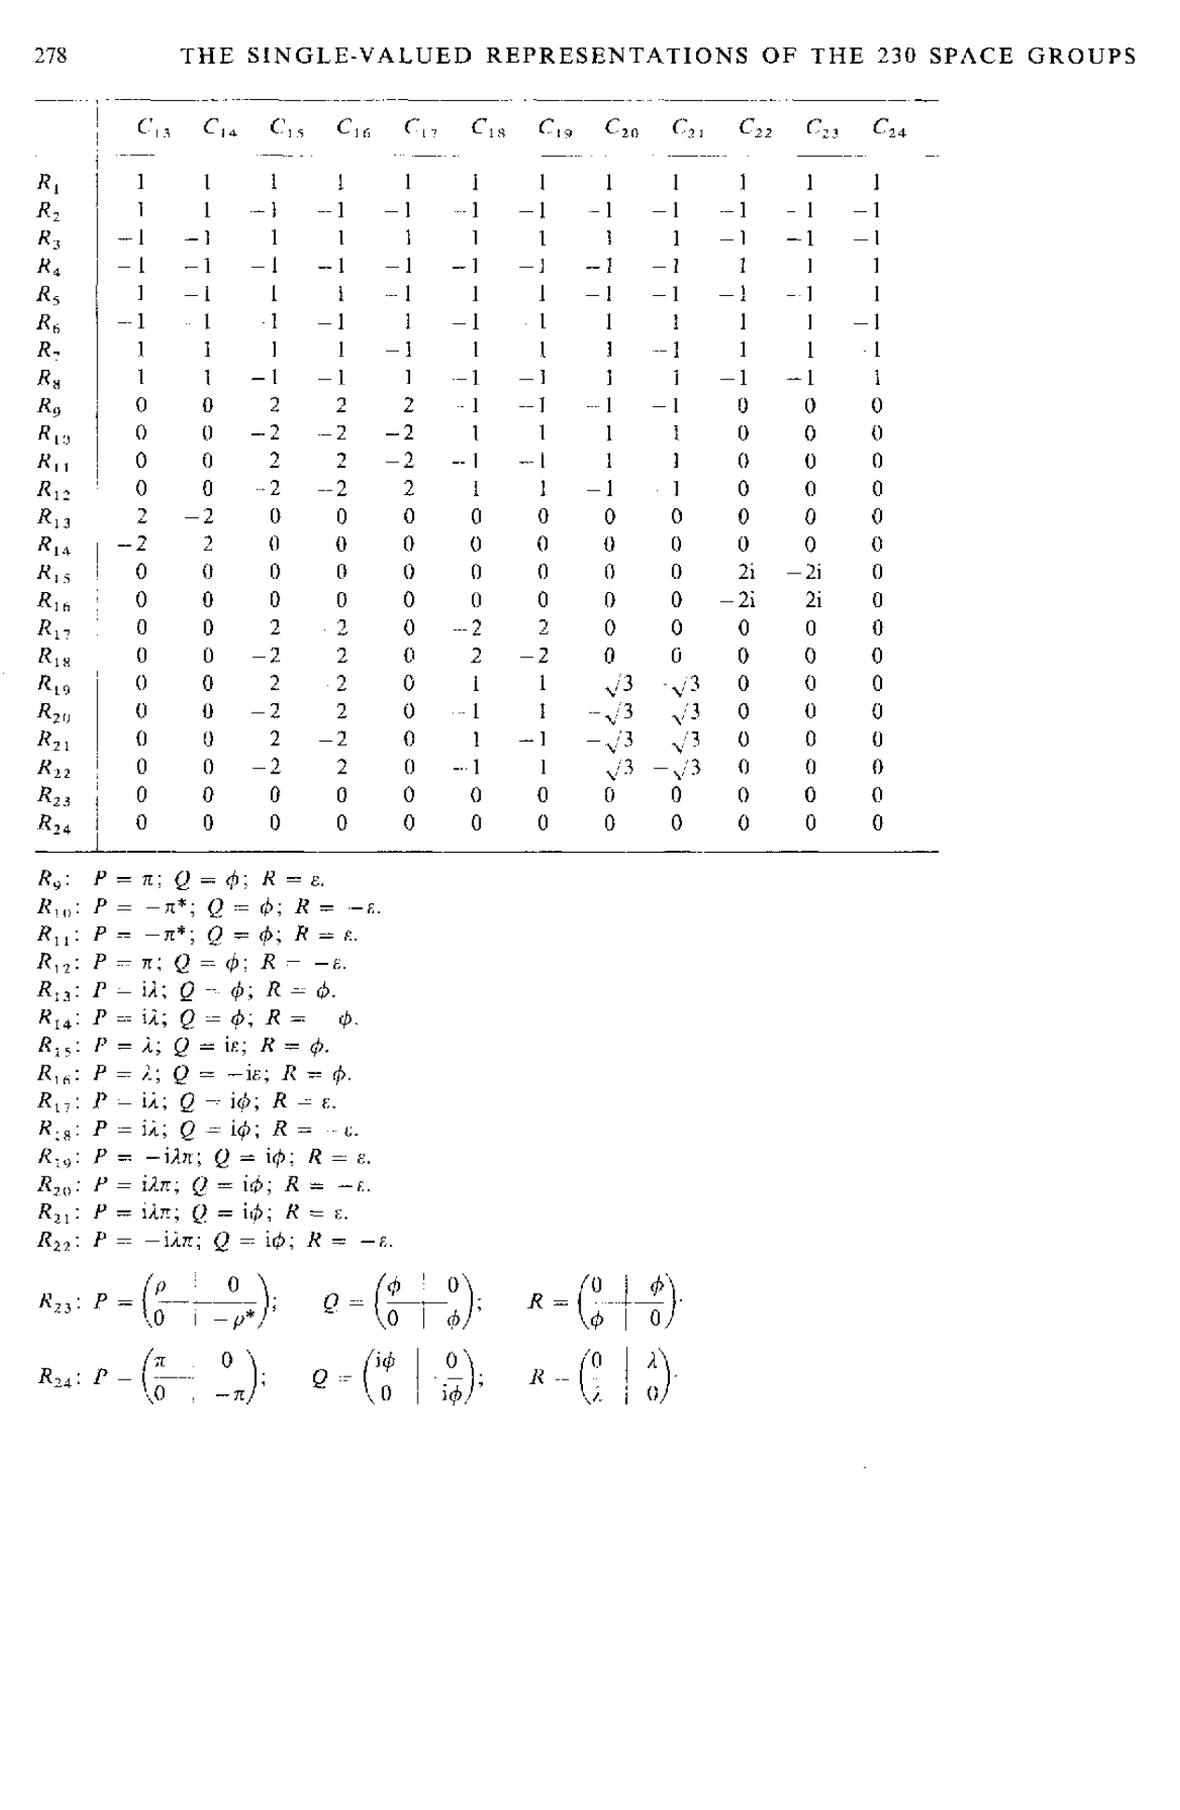
\includegraphics[width=0.86\textwidth]{c5_t51_p53.jpg}
\caption*{\textbf{表 5.1}（第 53 页，共 60 页；原书第 278 页）}
\end{figure}
\begin{figure}[H]
\centering
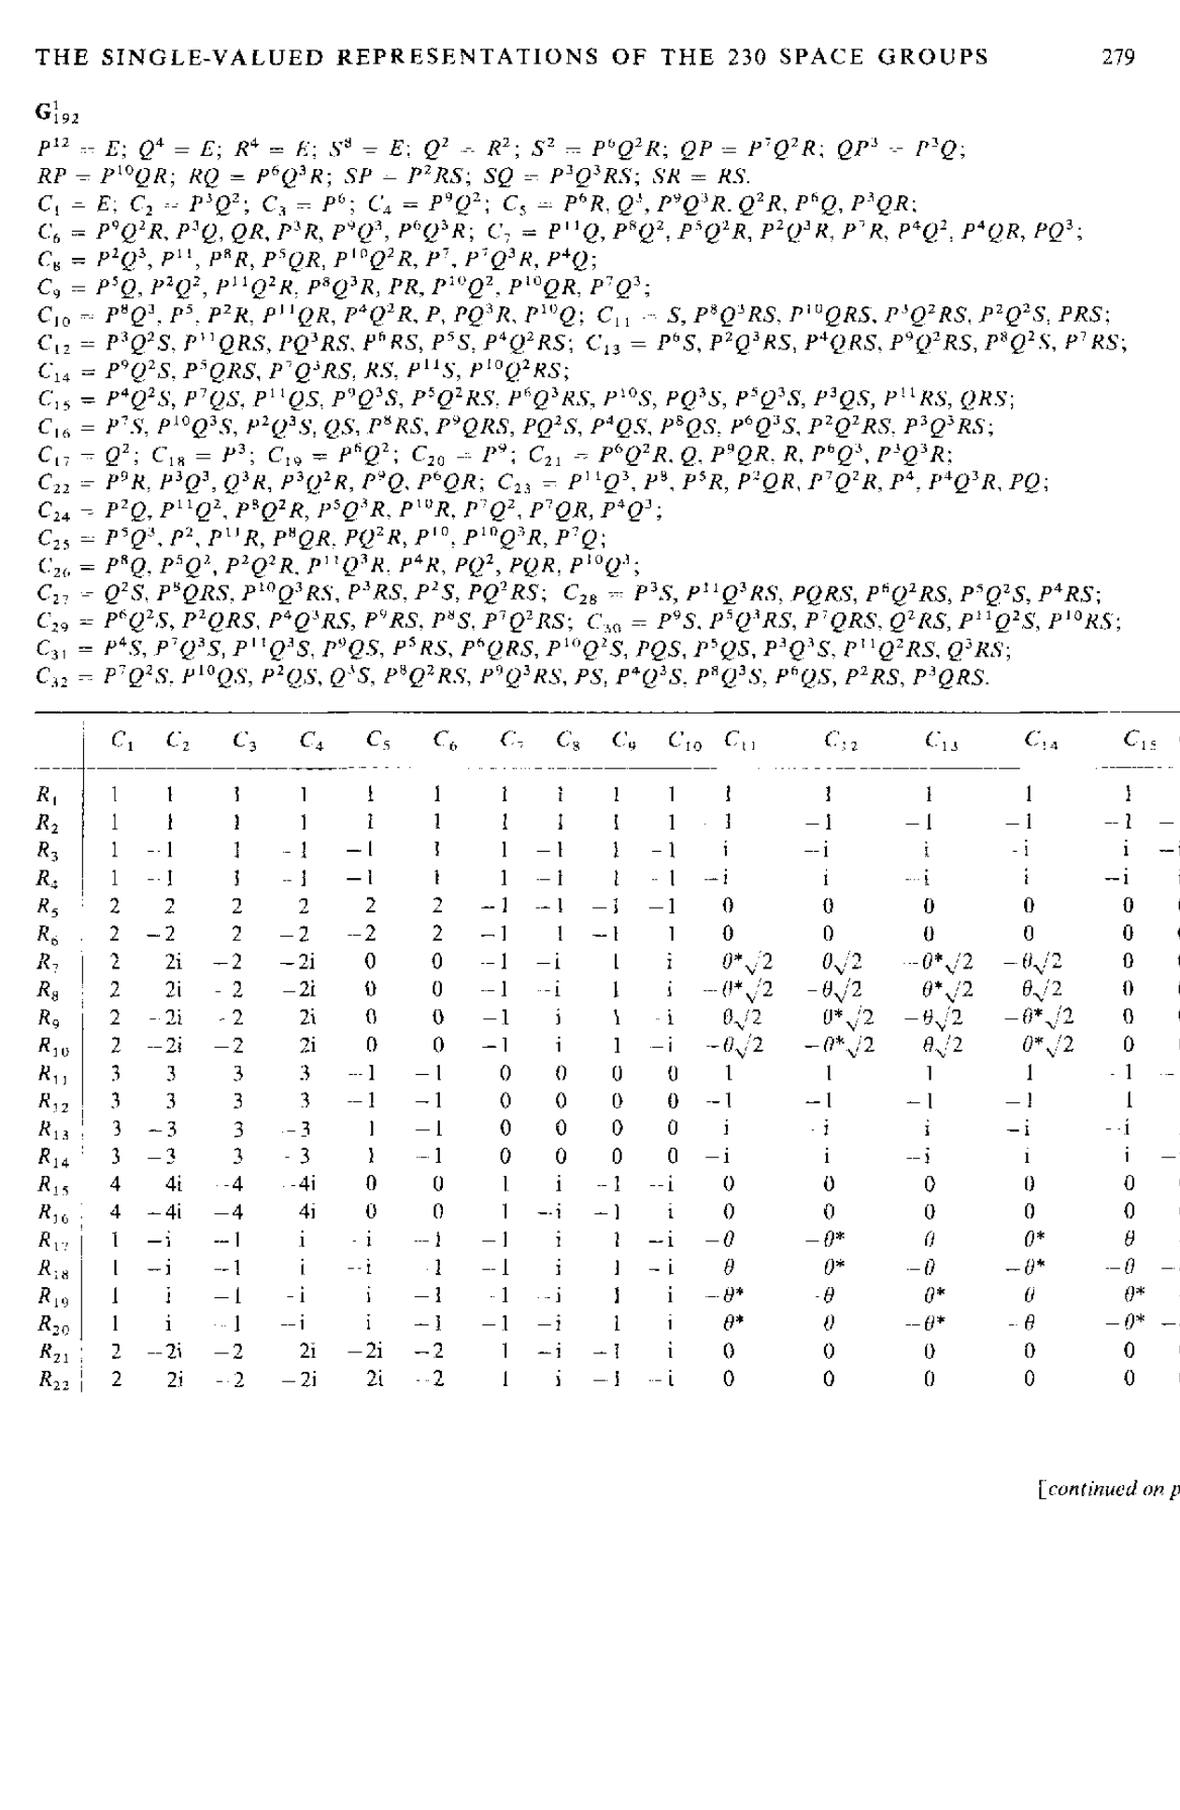
\includegraphics[width=0.86\textwidth]{c5_t51_p54.jpg}
\caption*{\textbf{表 5.1}（第 54 页，共 60 页；原书第 279 页）}
\end{figure}
\begin{figure}[H]
\centering
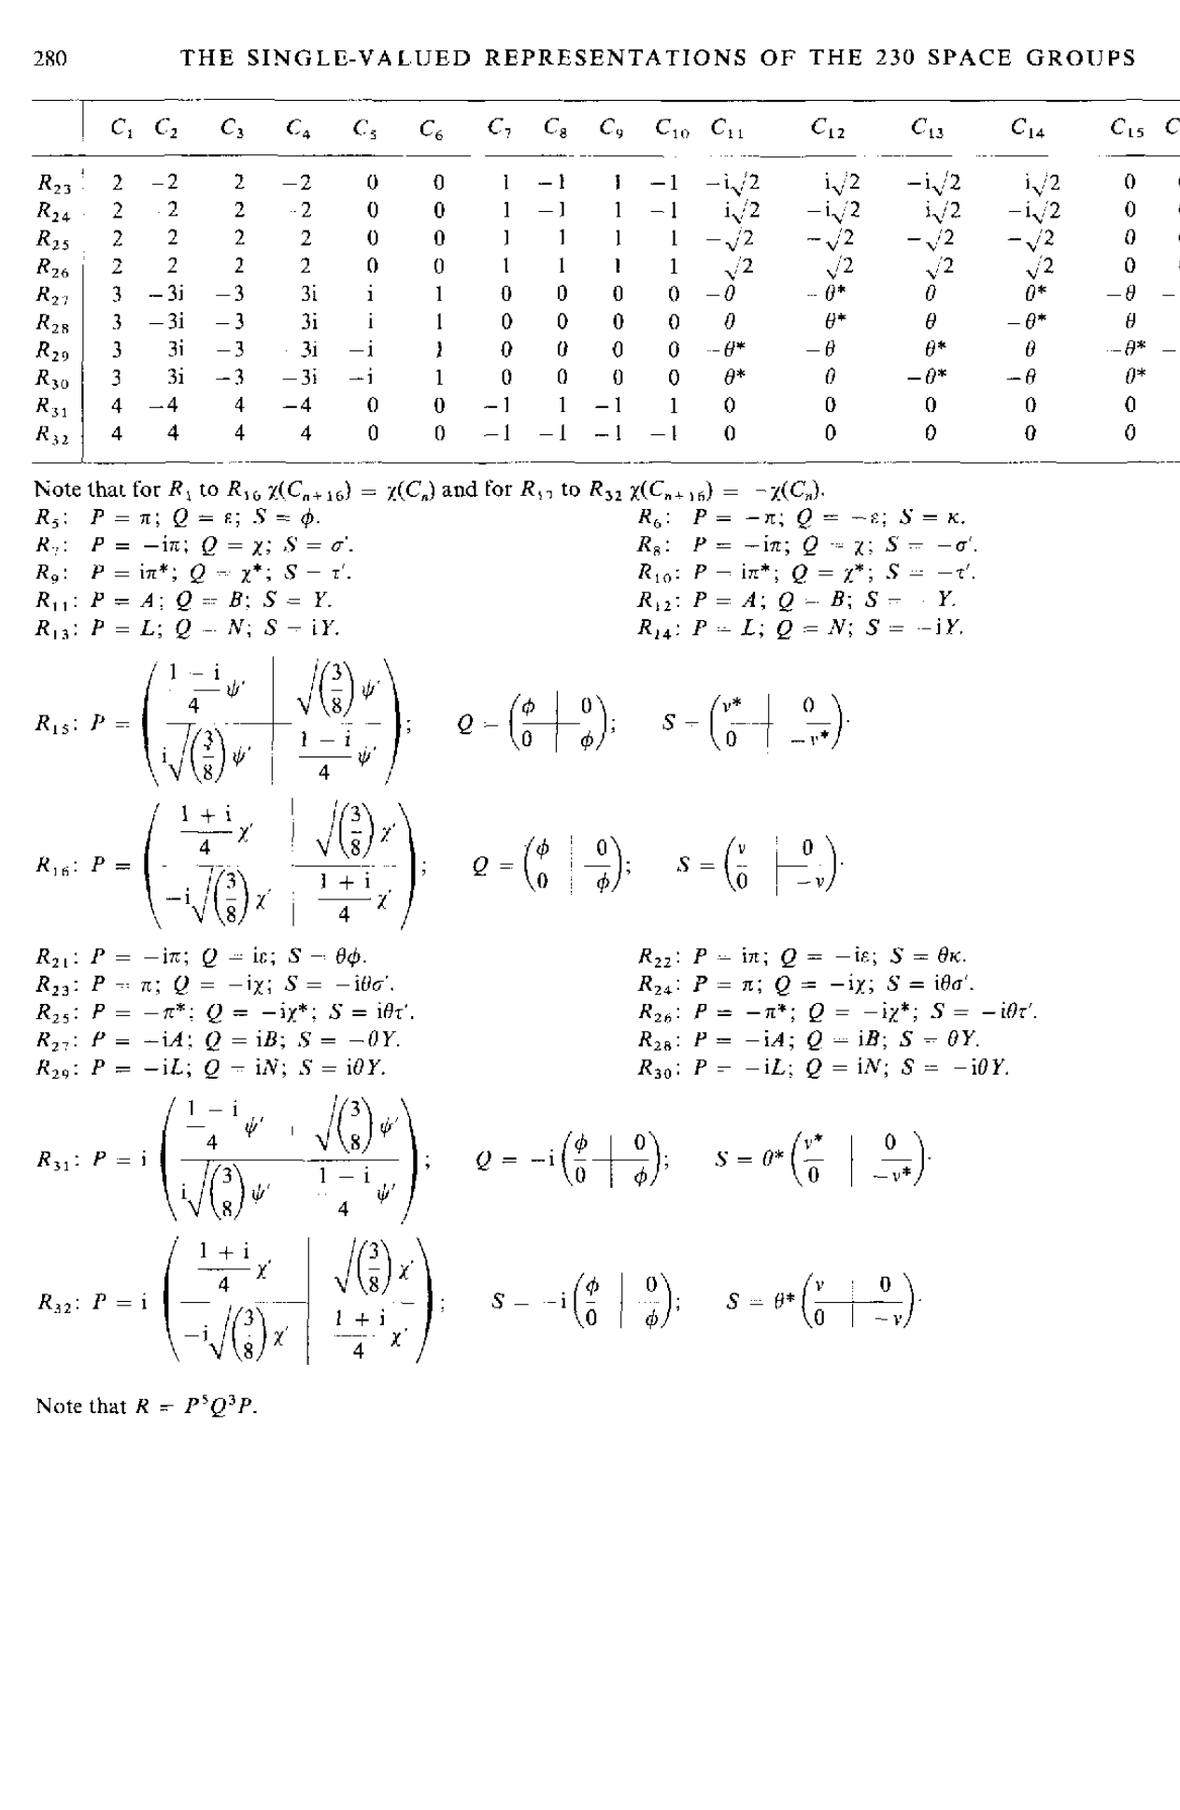
\includegraphics[width=0.86\textwidth]{c5_t51_p55.jpg}
\caption*{\textbf{表 5.1}（第 55 页，共 60 页；原书第 280 页）}
\end{figure}
\begin{figure}[H]
\centering
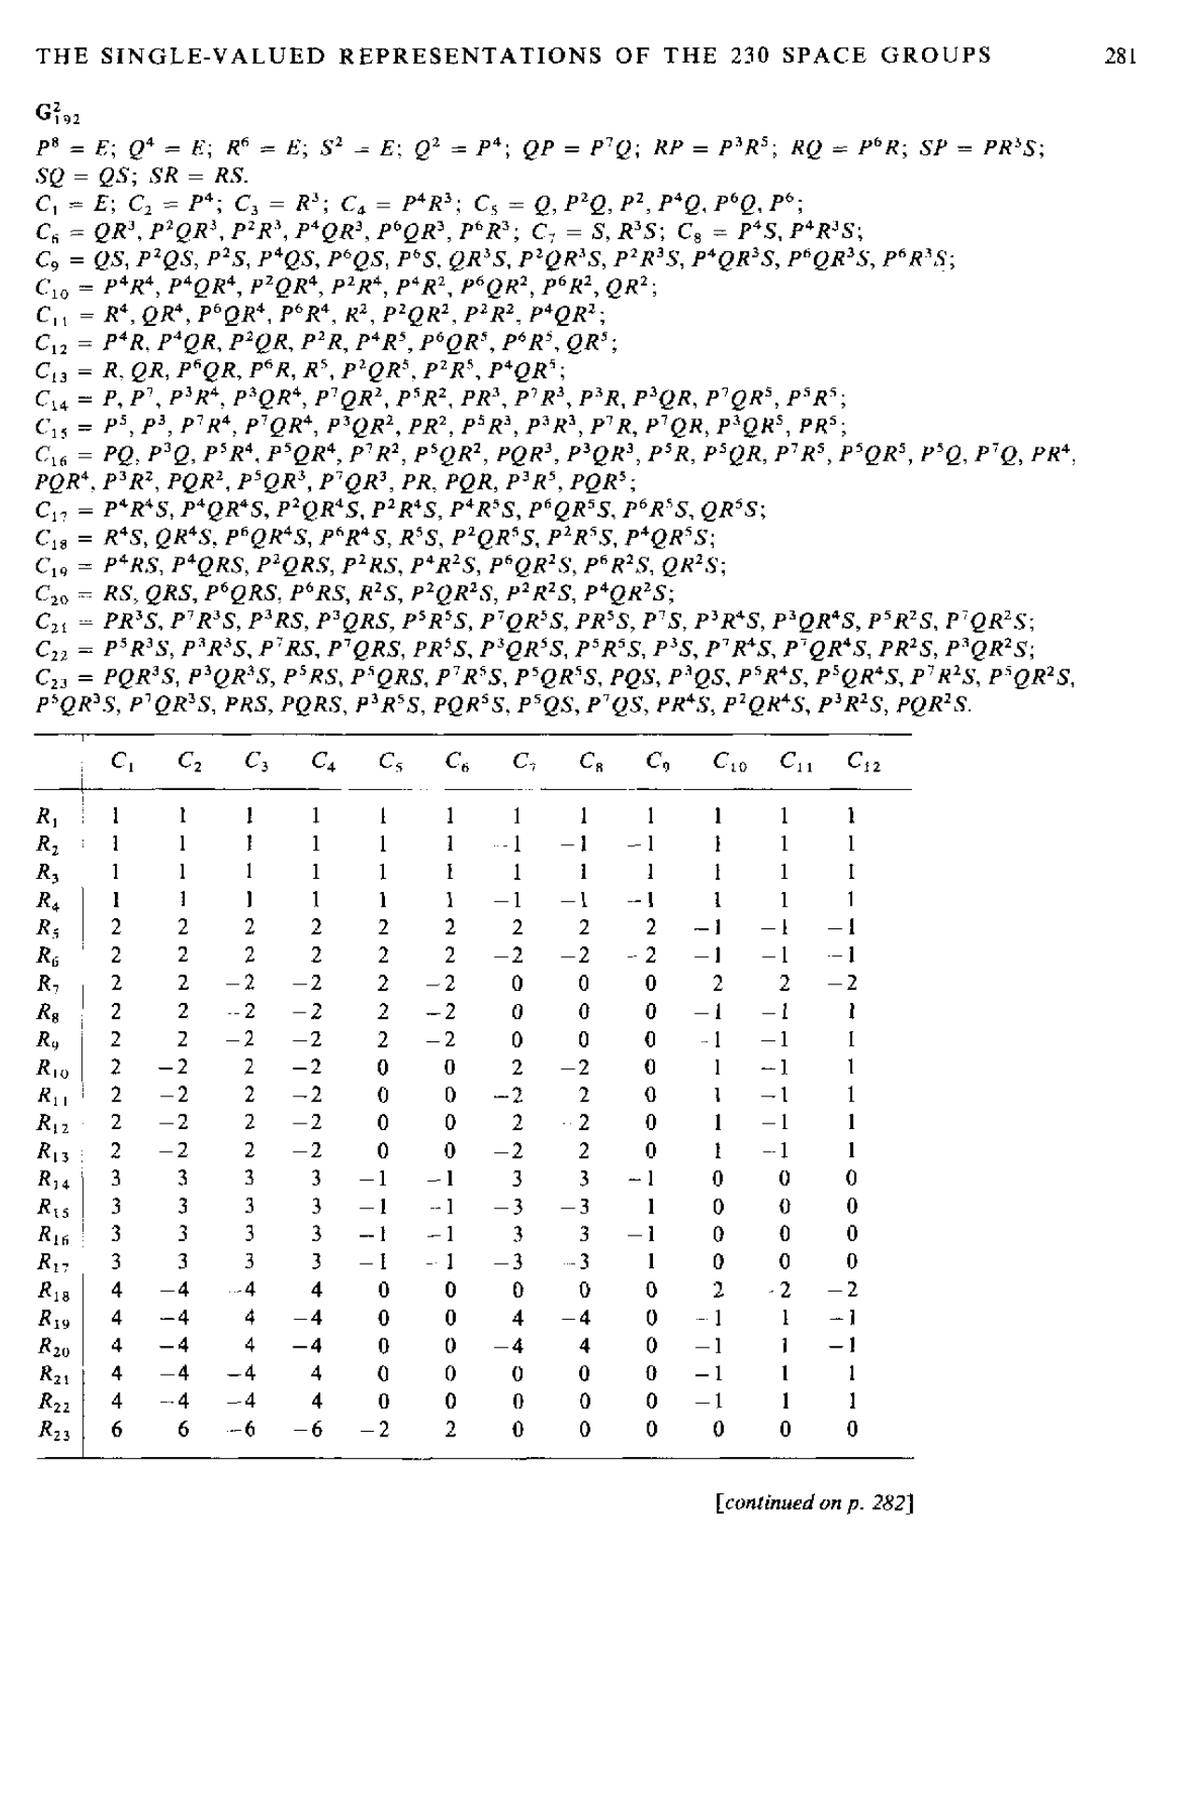
\includegraphics[width=0.86\textwidth]{c5_t51_p56.jpg}
\caption*{\textbf{表 5.1}（第 56 页，共 60 页；原书第 281 页）}
\end{figure}
\begin{figure}[H]
\centering
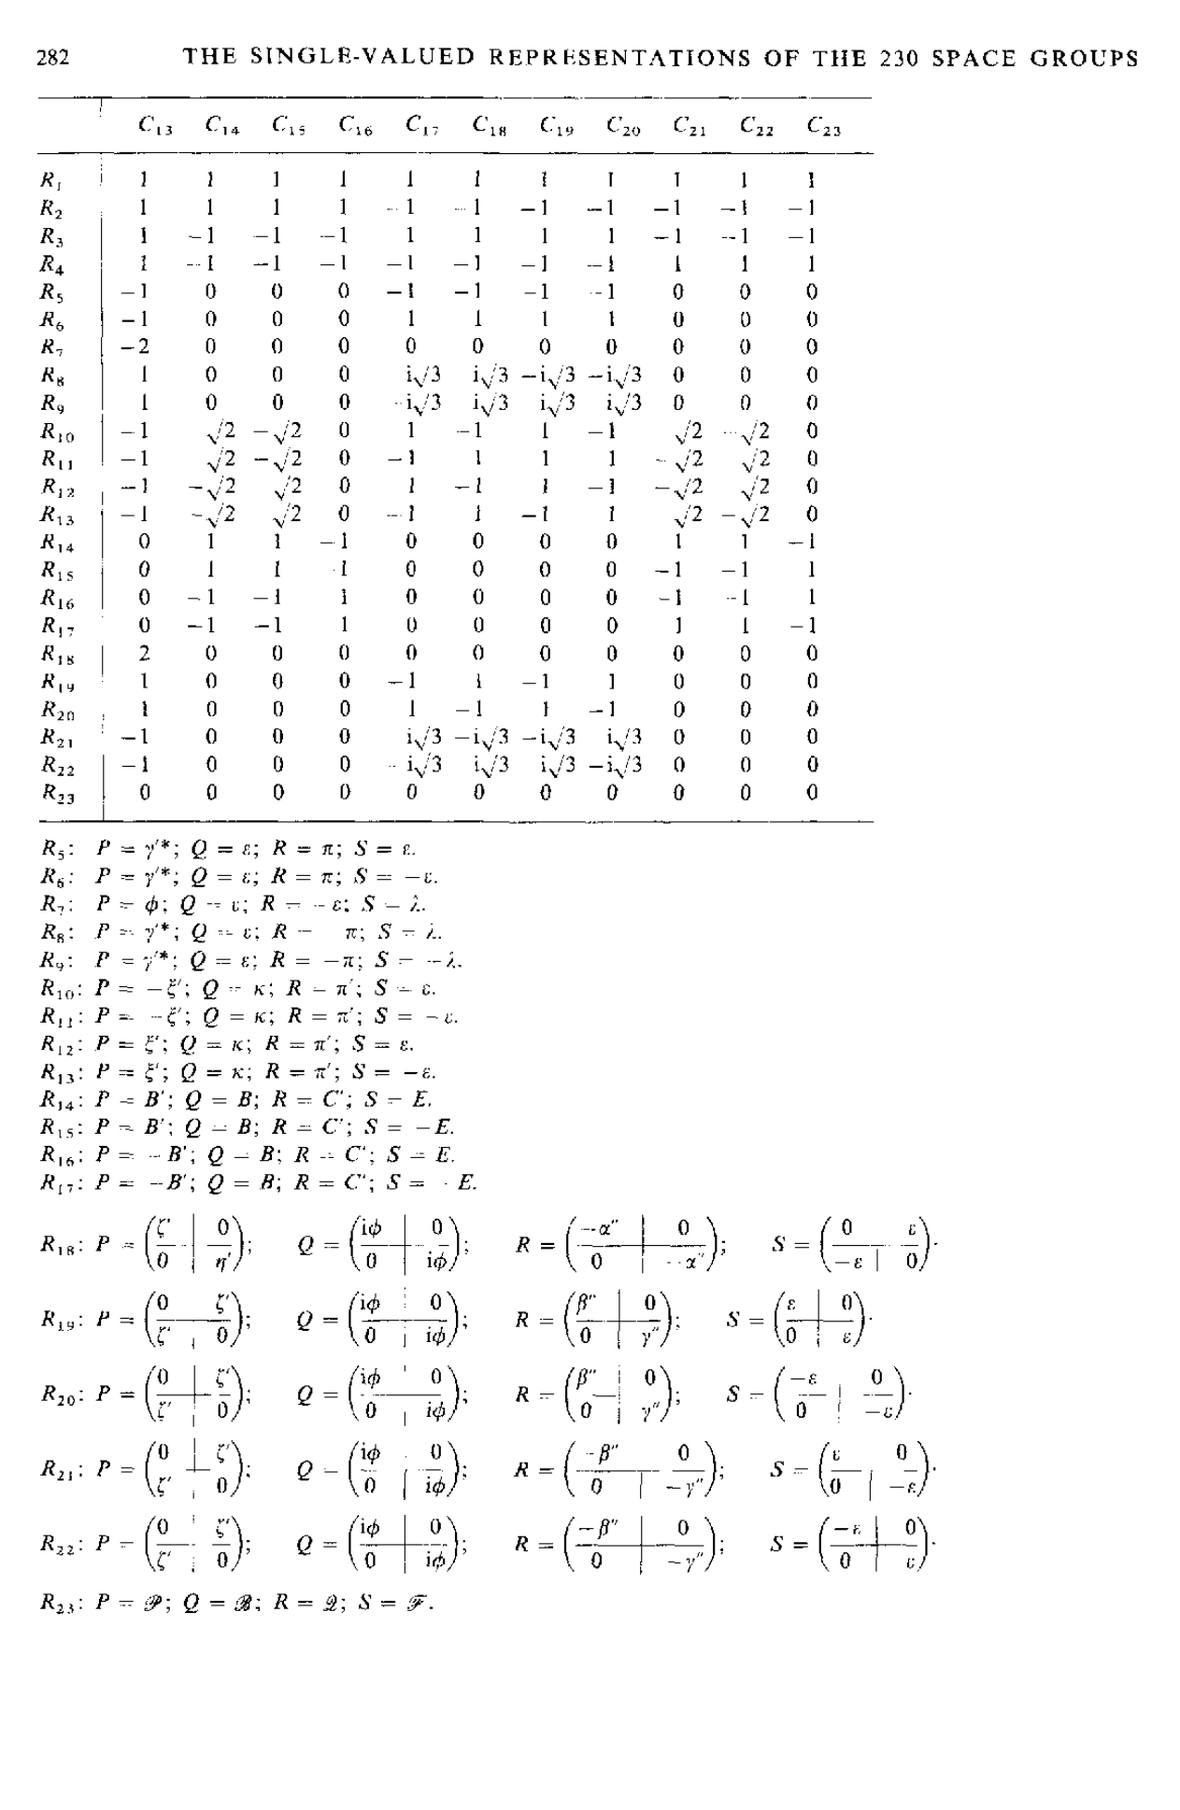
\includegraphics[width=0.86\textwidth]{c5_t51_p57.jpg}
\caption*{\textbf{表 5.1}（第 57 页，共 60 页；原书第 282 页）}
\end{figure}
\begin{figure}[H]
\centering
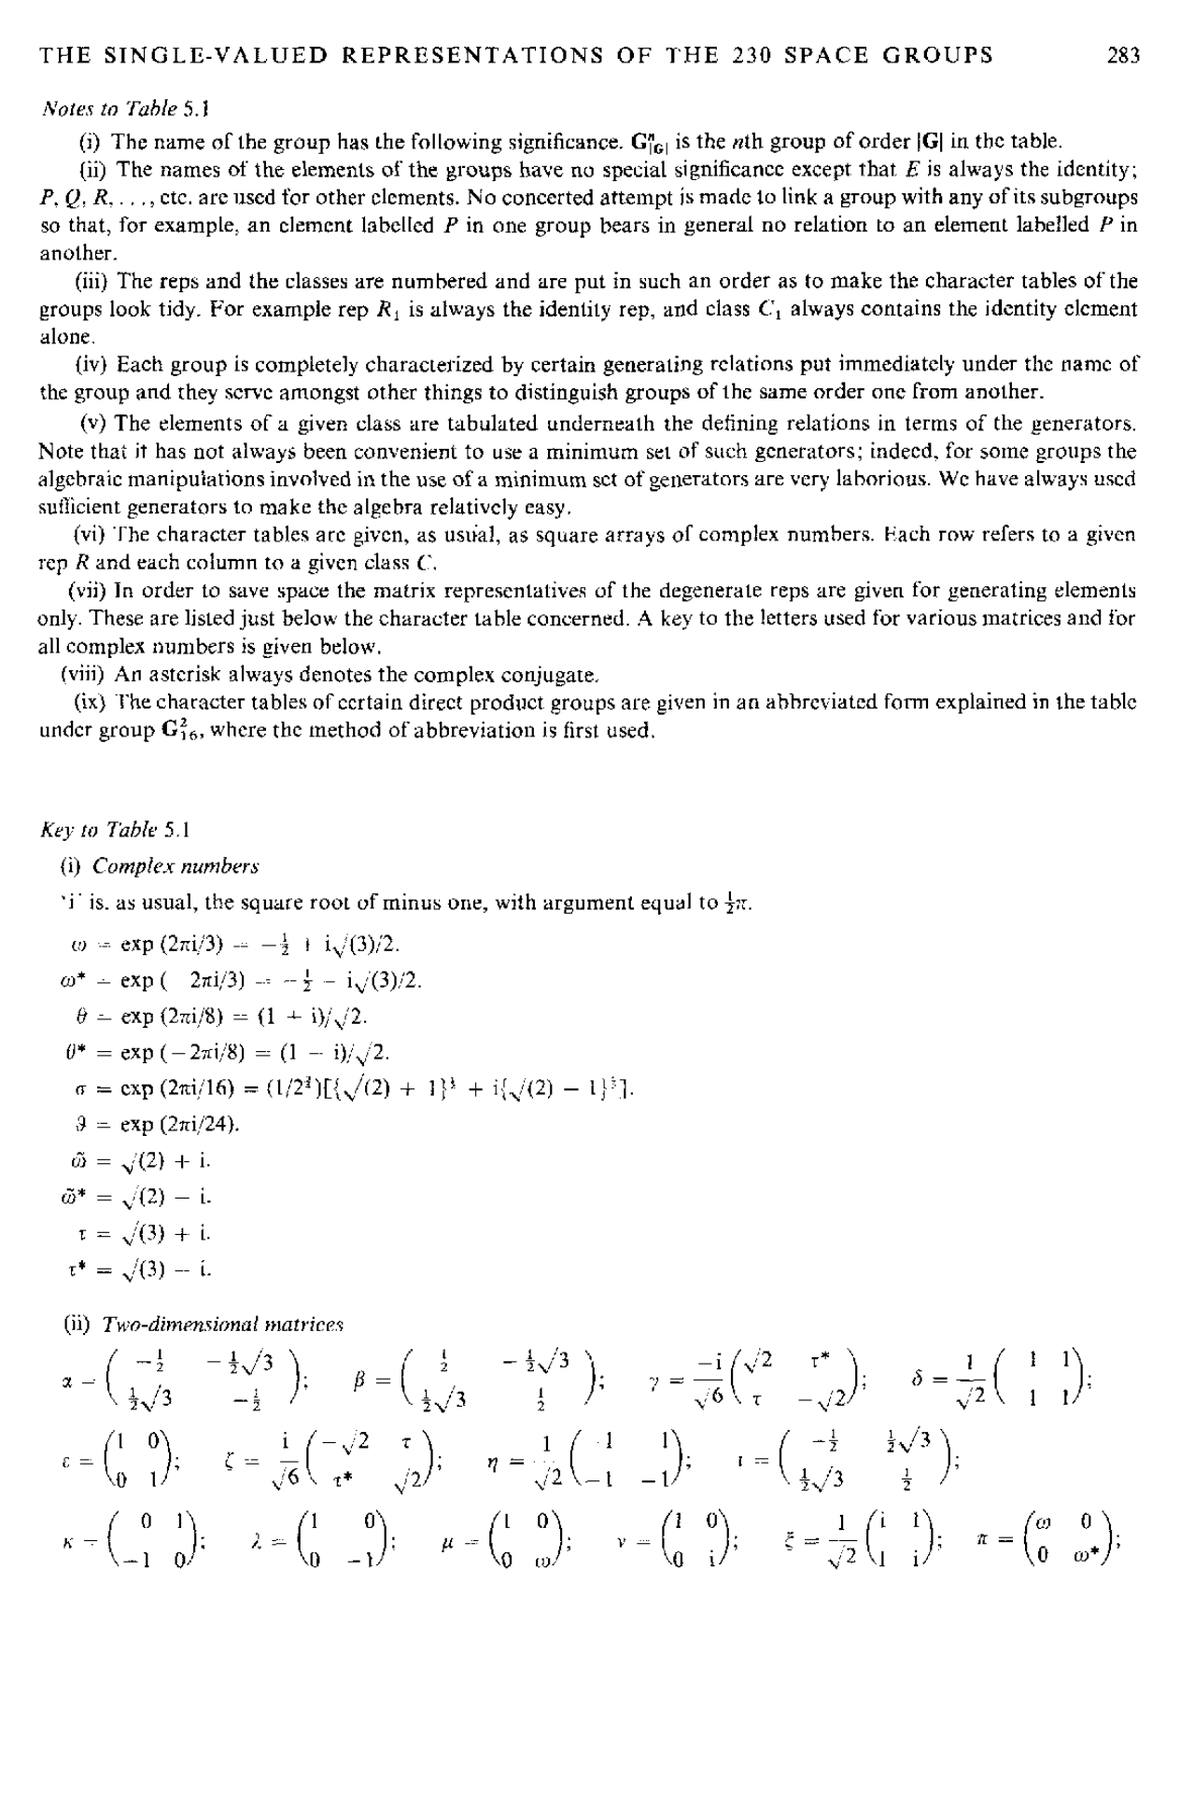
\includegraphics[width=0.86\textwidth]{c5_t51_p58.jpg}
\caption*{\textbf{表 5.1}（第 58 页，共 60 页；原书第 283 页）}
\end{figure}
\begin{figure}[H]
\centering
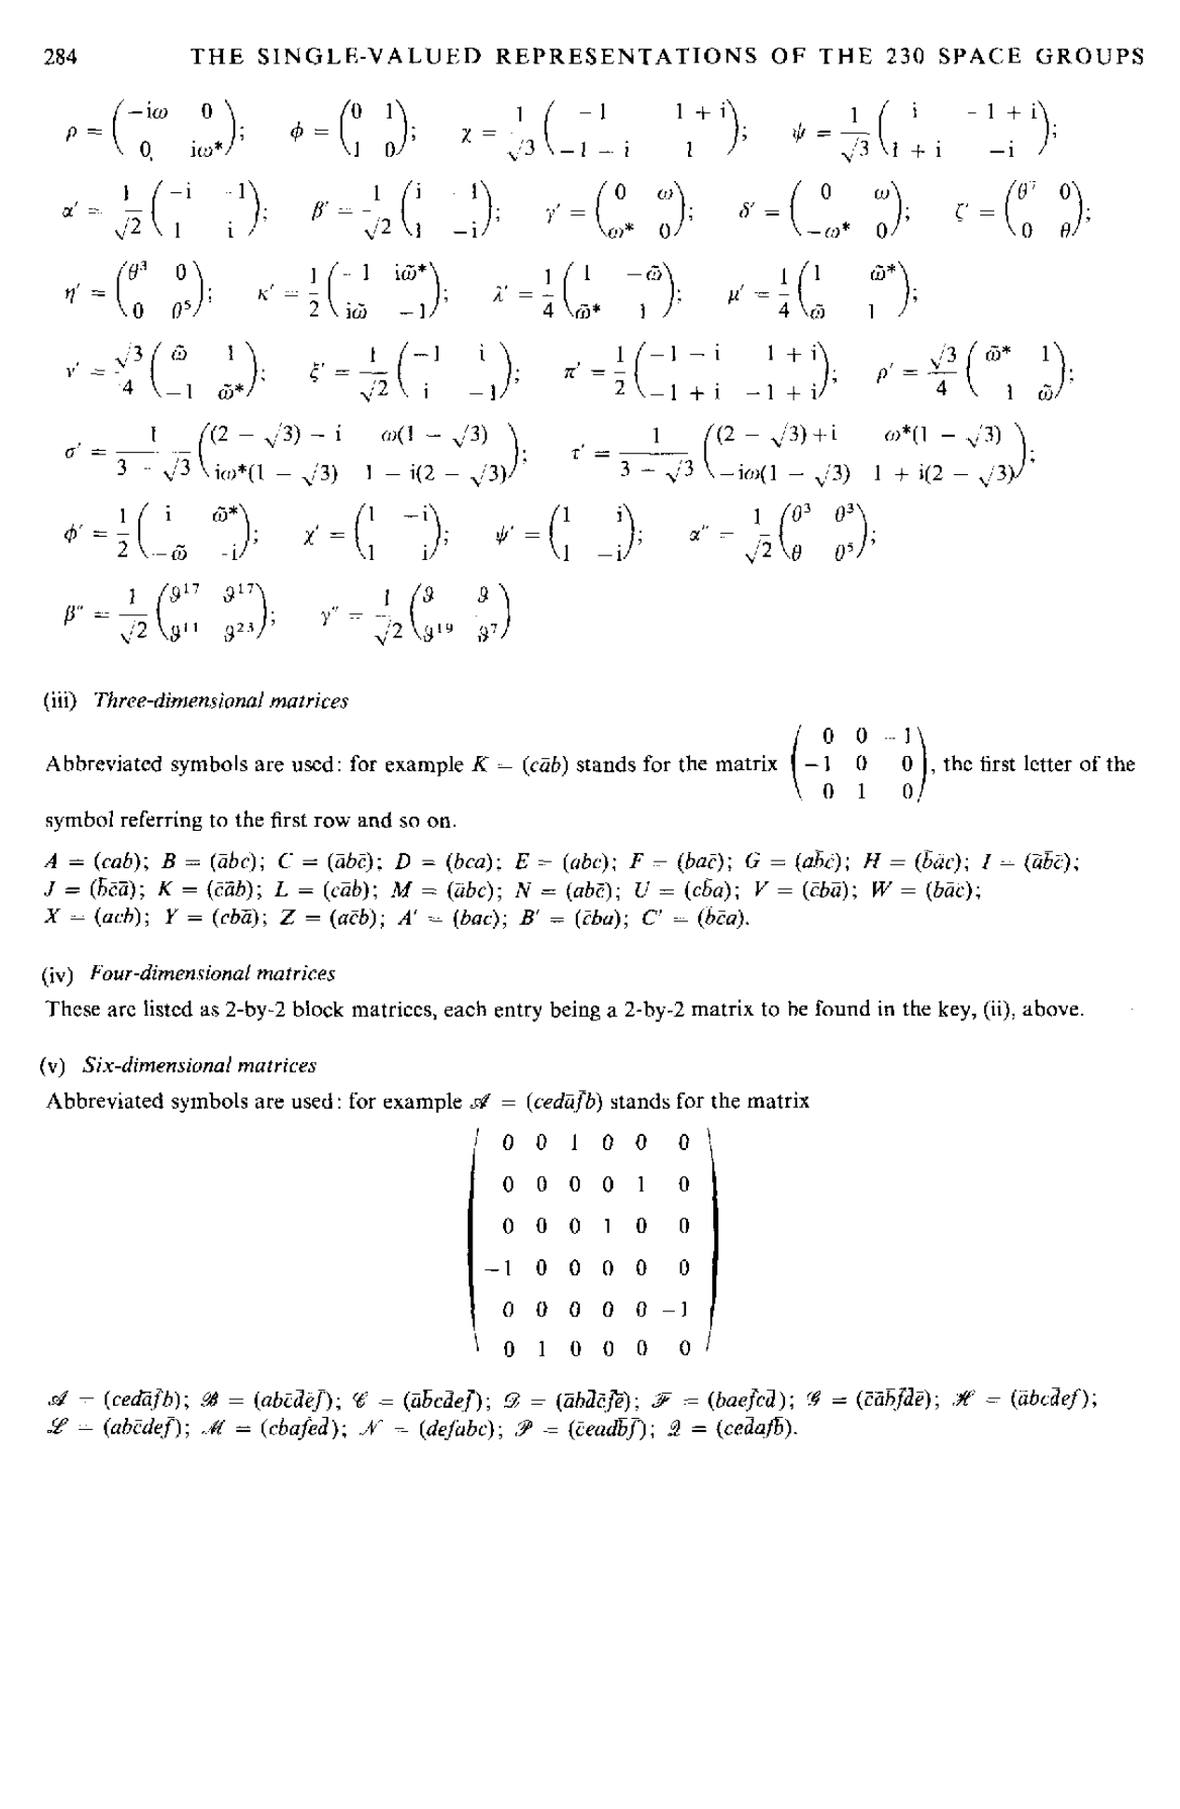
\includegraphics[width=0.86\textwidth]{c5_t51_p59.jpg}
\caption*{\textbf{表 5.1}（第 59 页，共 60 页；原书第 284 页）}
\end{figure}
\begin{figure}[H]
\centering
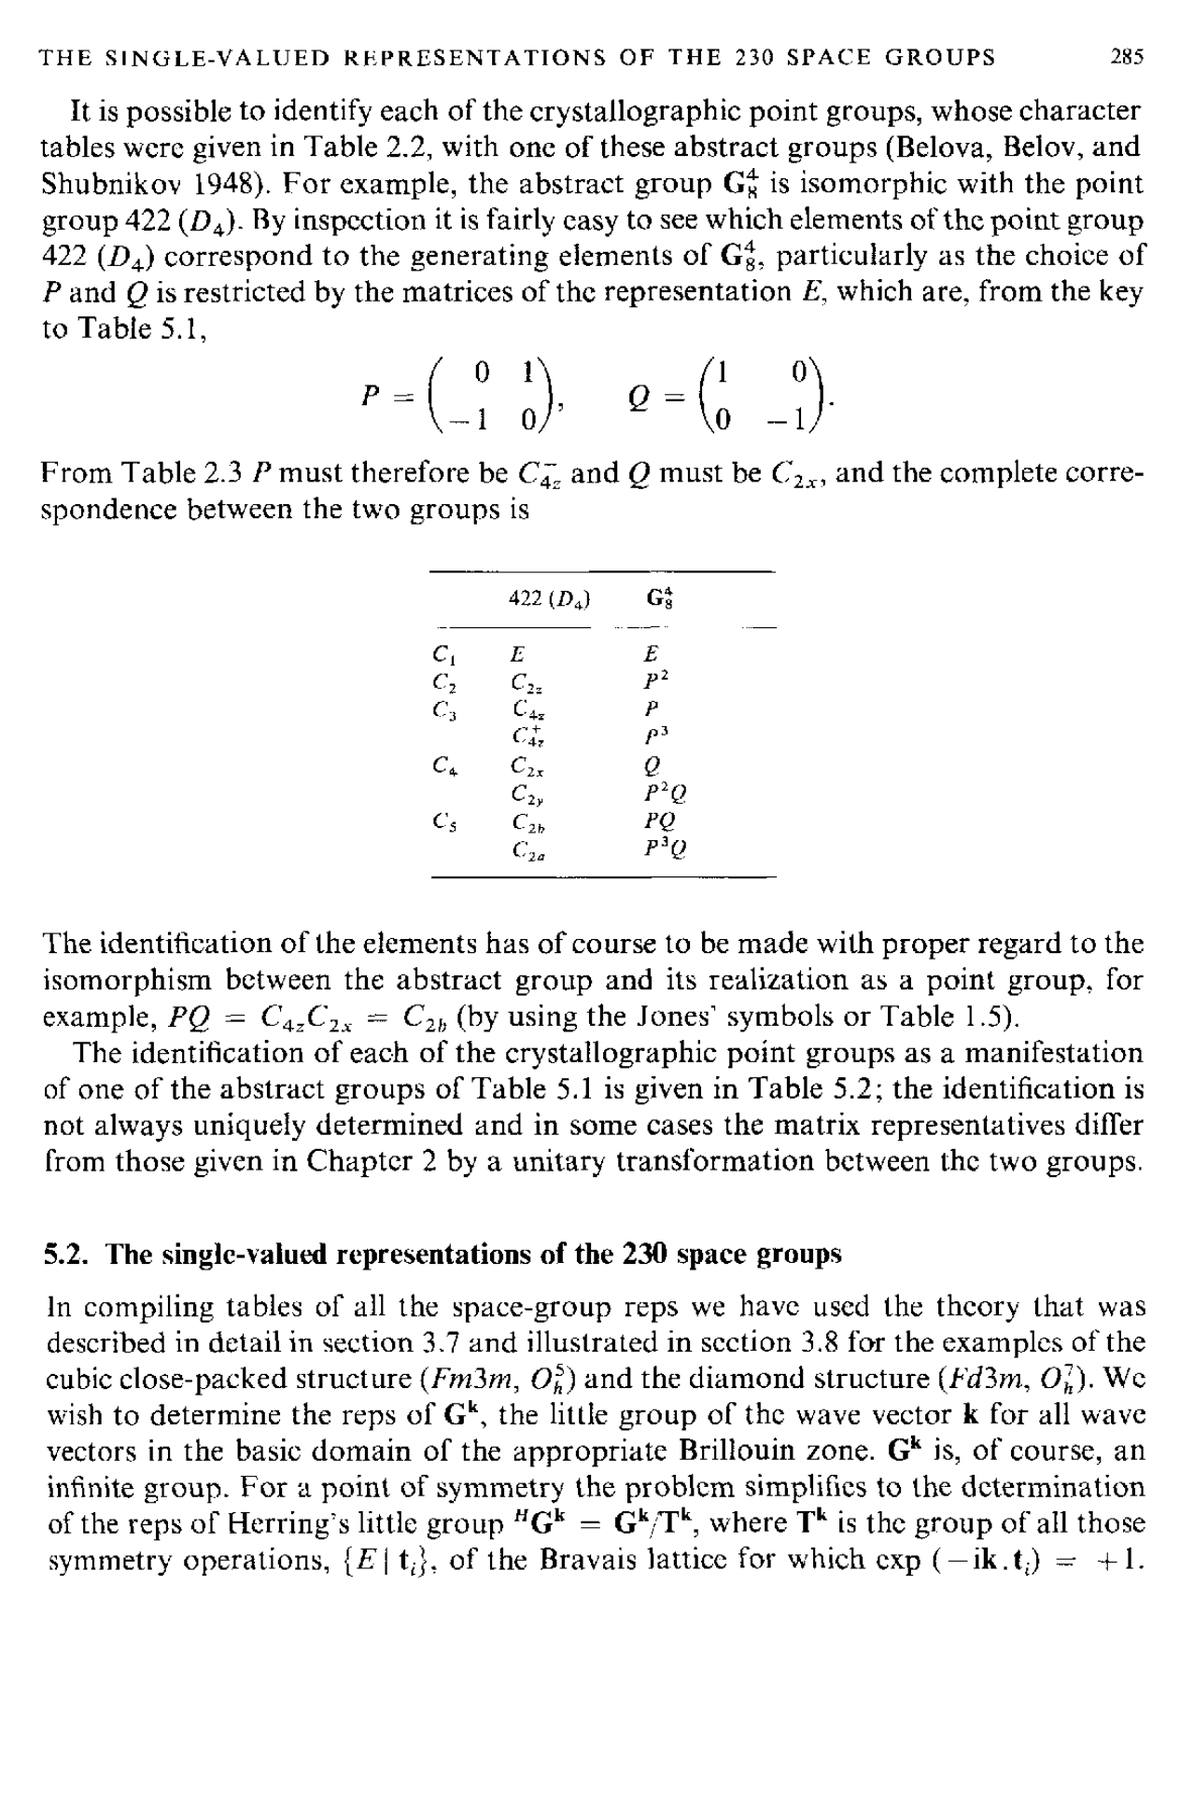
\includegraphics[width=0.86\textwidth]{c5_t51_p60.jpg}
\caption*{\textbf{表 5.1}（第 60 页，共 60 页；原书第 285 页）}
\end{figure}

可以把（其特征标表已在表 2.2 中给出的）每个晶体学点群与这些抽象群之一对应起来（Belova, Belov, and Shubnikov 1948）。例如，抽象群 $\mathbf{G}^{4}_{8}$ 同构于点群 $422\ (D_{4})$。通过观察不难看出点群 $422\ (D_{4})$ 的哪些元素对应于 $\mathbf{G}^{4}_{8}$ 的生成元，特别是因为 $P$ 与 $Q$ 的选取受到表示 $E$ 的矩阵的限制——由表 5.1 的钥匙（key），
\begin{equation*}
P = \begin{pmatrix} 0 & 1\\ -1 & 0 \end{pmatrix}, \quad Q = \begin{pmatrix} 1 & 0\\ 0 & -1 \end{pmatrix}.
\end{equation*}
因此由表 2.3，$P$ 必是 $C^{-}_{4z}$，$Q$ 必是 $C_{2x}$，于是两个群之间的完整对应为
\begin{center}
\begin{tabular}{lcc}
 & $422\ (D_{4})$ & $\mathbf{G}^{4}_{8}$\\
$C_{1}$ & $E$ & $E$\\
$C_{2}$ & $C_{2z}$ & $P^{2}$\\
$C_{3}$ & $\begin{array}{c}C^{-}_{4z}\\ C^{+}_{4z}\end{array}$ & $\begin{array}{c}P\\ P^{3}\end{array}$\\
$C_{4}$ & $\begin{array}{c}C_{2x}\\ C_{2y}\end{array}$ & $\begin{array}{c}Q\\ P^{2}Q\end{array}$\\
$C_{5}$ & $\begin{array}{c}C_{2b}\\ C_{2a}\end{array}$ & $\begin{array}{c}PQ\\ P^{3}Q\end{array}$
\end{tabular}
\end{center}
当然，元素的认定必须恰当顾及抽象群与其作为点群的实现之间的同构，例如 $PQ = C^{-}_{4z}C_{2x} = C_{2b}$（用 Jones 符号或表 1.5）。

每个晶体学点群作为表 5.1 中某一抽象群的一种体现的认定由表 5.2 给出；这一认定并不总是唯一的，且某些情形下矩阵代表与第二章所给者相差两个群之间的一个幺正变换。

% 5.2 230 个空间群的单值表示
\section{230 个空间群的单值表示}

在编制所有空间群的表示表时，我们用的是 3.7 节详述、3.8 节以立方密堆积结构（$Fm3m$, $O^{5}_{h}$）与金刚石结构（$Fd3m$, $O^{7}_{h}$）为例演示过的理论。我们要确定的是 $\mathbf{G}^{\mathbf{k}}$——波矢 $\mathbf{k}$ 的小群——对相应布里渊区基本域中所有波矢的表示。当然 $\mathbf{G}^{\mathbf{k}}$ 是无限群。对对称点，问题简化为求 Herring 小群 ${}^{H}\mathbf{G}^{\mathbf{k}} = \mathbf{G}^{\mathbf{k}}/\mathbf{T}^{\mathbf{k}}$ 的表示，其中 $\mathbf{T}^{\mathbf{k}}$ 是布拉维格子那些满足 $\exp(-\mathrm{i}\mathbf{k} \cdot \mathbf{t}_{i}) = +1$ 的对称操作 $\{E \mid \mathbf{t}_{i}\}$ 构成的群；$\mathbf{T}^{\mathbf{k}}$ 是布拉维格子全部平移对称操作群 $\mathbf{T}$ 的子群。群 ${}^{H}\mathbf{G}^{\mathbf{k}}$ 的元素可以由表 3.6 与 3.7 确定，然后通过直接相乘 Seitz 空间群符号——每当 $\exp(-\mathrm{i}\mathbf{k} \cdot \mathbf{t}_{i}) = +1$ 时把 $\{E \mid \mathbf{t}_{i}\}$ 换成 $\{E \mid \mathbf{0}\}$——得到 ${}^{H}\mathbf{G}^{\mathbf{k}}$ 的群乘法表。我们称 ${}^{H}\mathbf{G}^{\mathbf{k}}$ 为 Herring 小群，因为这种处理对称点的方法最初由 Herring (1942) 用于确定六角密堆积与金刚石结构的空间群特征标表。这个群随后可以辨认为表 5.1 中的抽象群 $\mathbf{G}^{n}_{|\mathbf{G}|}$ 之一，从而容易辨认可作为小表示（即满足式 (3.4.3) 的表示）的 $\mathbf{G}^{n}_{|\mathbf{G}|}$ 的相应表示。对对称线上的 $\mathbf{k}$，我们必须通过求中央延拓群 $\overline{\mathbf{G}}^{\mathbf{k}*}$ 的射影表示来得到 $\mathbf{G}^{\mathbf{k}}$ 的表示。对此类 $\mathbf{k}$，$\mathbf{T}/\mathbf{T}^{\mathbf{k}}$ 不含有限个元素，因此试图从有限群的表示确定 $\mathbf{G}^{\mathbf{k}}$ 的小表示时，不能有效地使用 $\mathbf{G}^{\mathbf{k}}/\mathbf{T}^{\mathbf{k}}$（它现在是无限群）；为了找到一个合适的有限群，必须改用中央延拓群 $\overline{\mathbf{G}}^{\mathbf{k}*}$。$\overline{\mathbf{G}}^{\mathbf{k}*}$ 元素的群乘法表用乘法规则确定。于是可以把 $\overline{\mathbf{G}}^{\mathbf{k}*}$ 辨认为表 5.1 的某个抽象群，并辨认同它的小表示相应的那些表示。

可以把每个晶体学点群辨认为某个抽象群的一种体现（表 5.2）。表 5.2 的第 3 列给出与该点群的类相对应的抽象群生成元。例如对 $432\ (O)$，星 $A$ 的小陪群为 $32'\ (D'_{3})$，等等。

\begin{figure}[H]
\centering
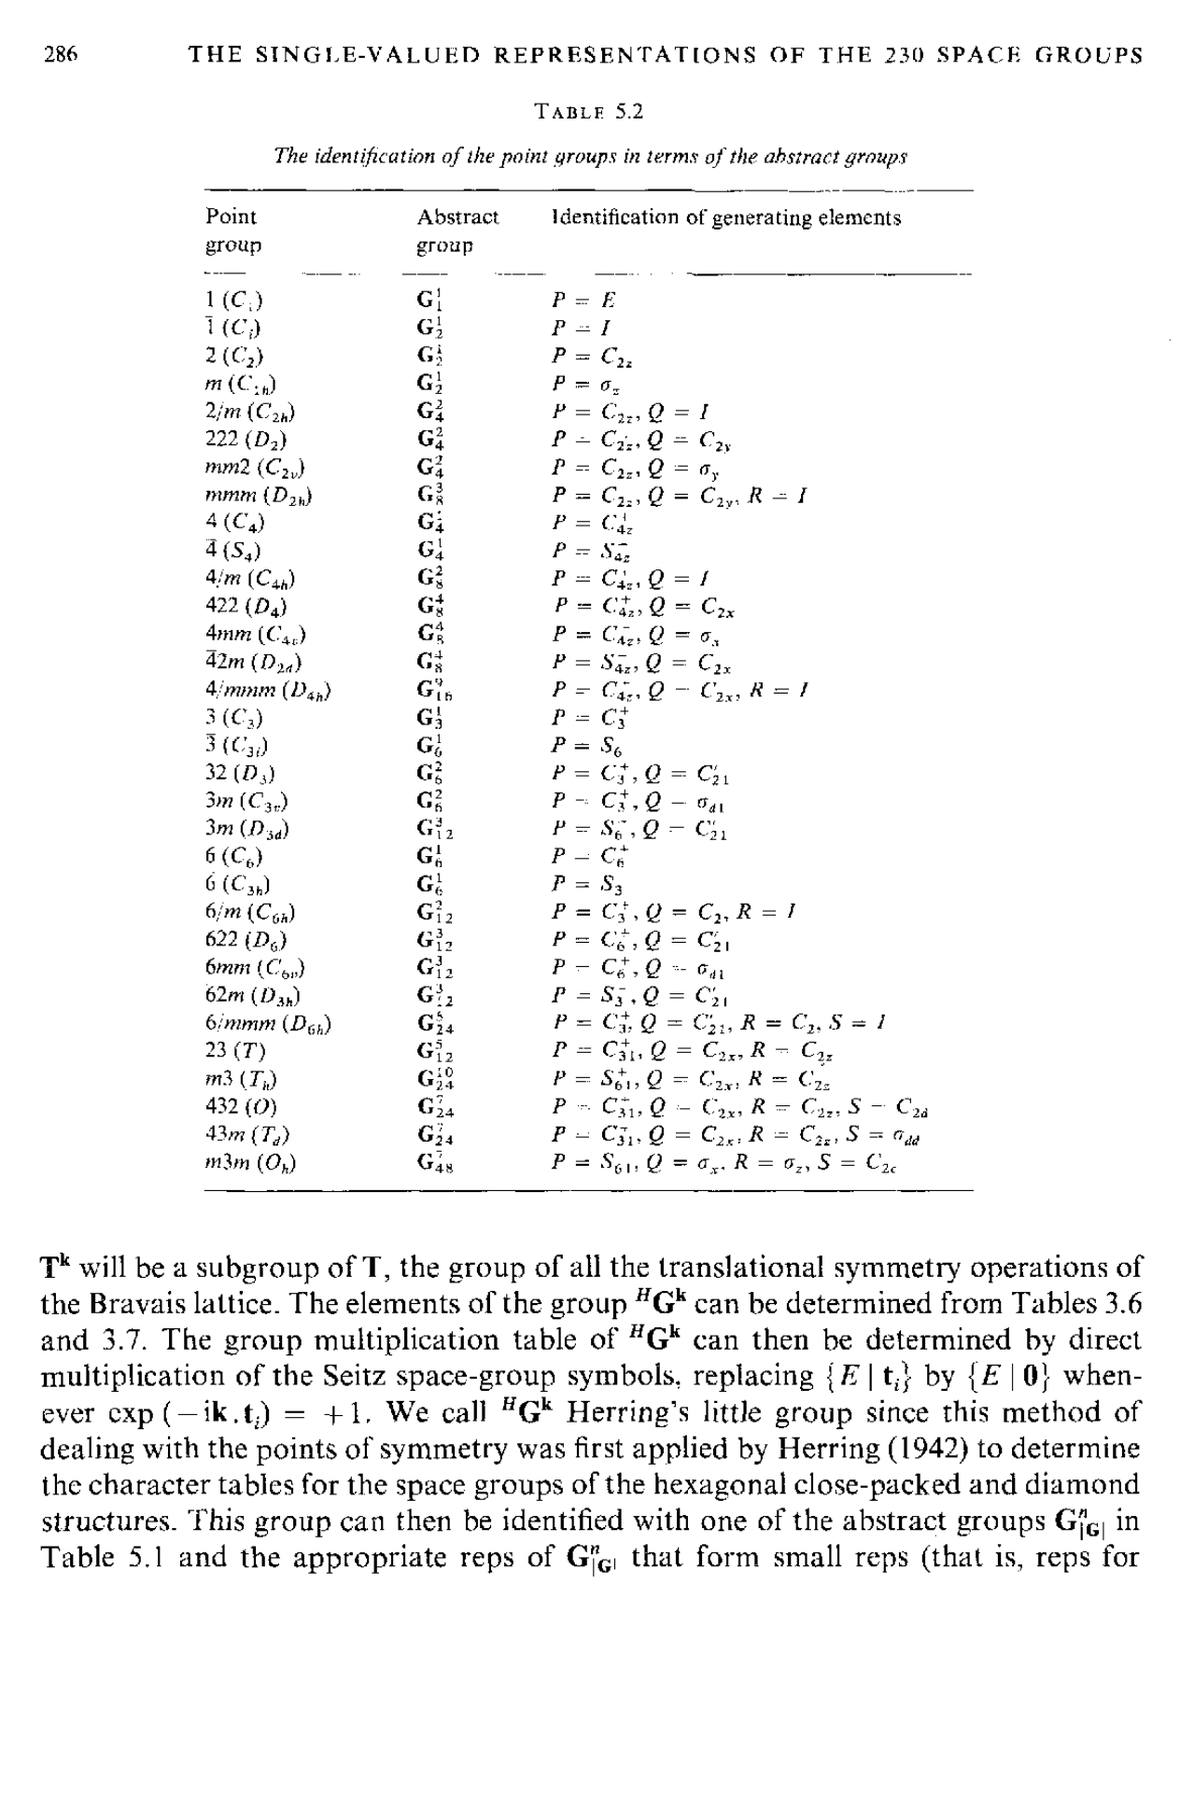
\includegraphics[width=0.86\textwidth]{c5_52_p299.jpg}
\caption*{\textbf{表 5.2}\ 用抽象群辨认点群（原书第 286 页扫描）。}
\end{figure}
\begin{figure}[H]
\centering
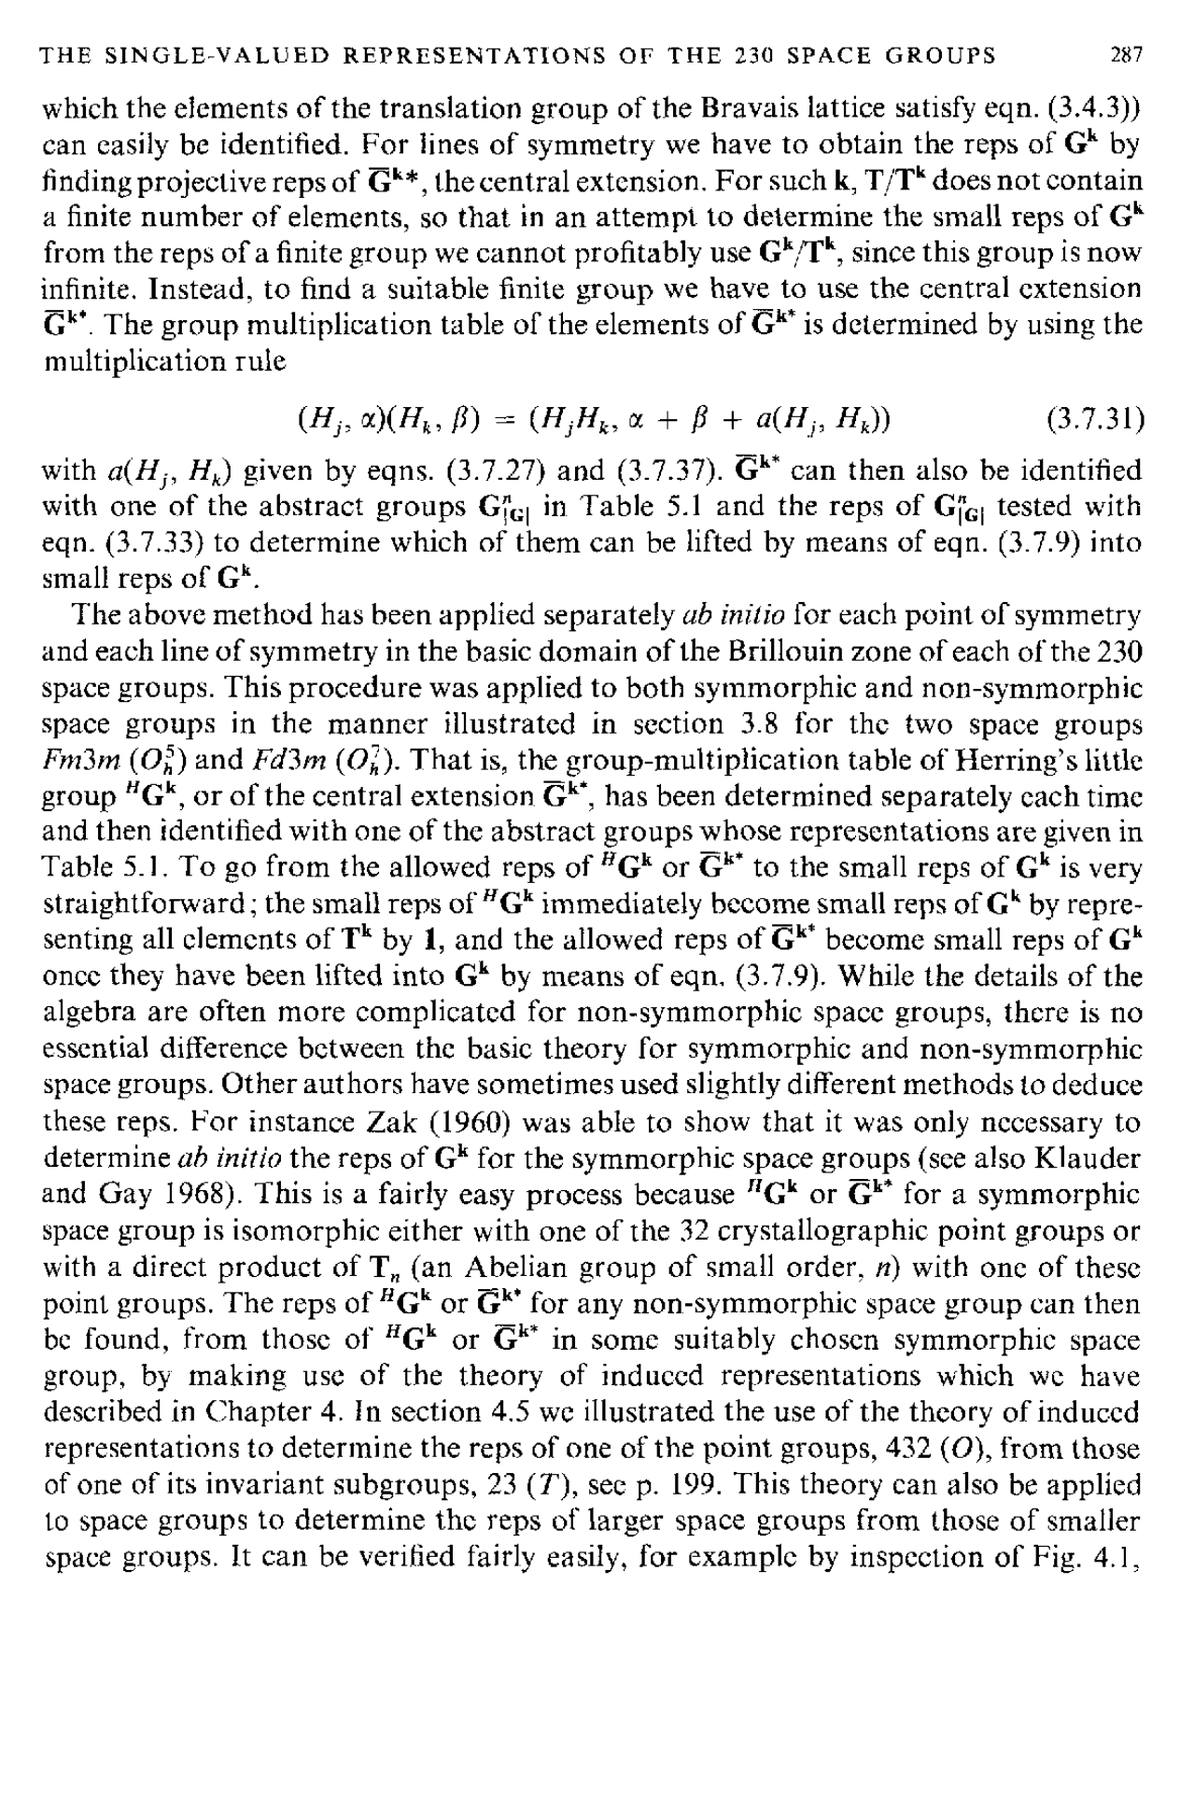
\includegraphics[width=0.86\textwidth]{c5_52_p300.jpg}
\caption*{表 5.2（续）与表 5.3（原书第 287 页扫描）。}
\end{figure}
\begin{figure}[H]
\centering
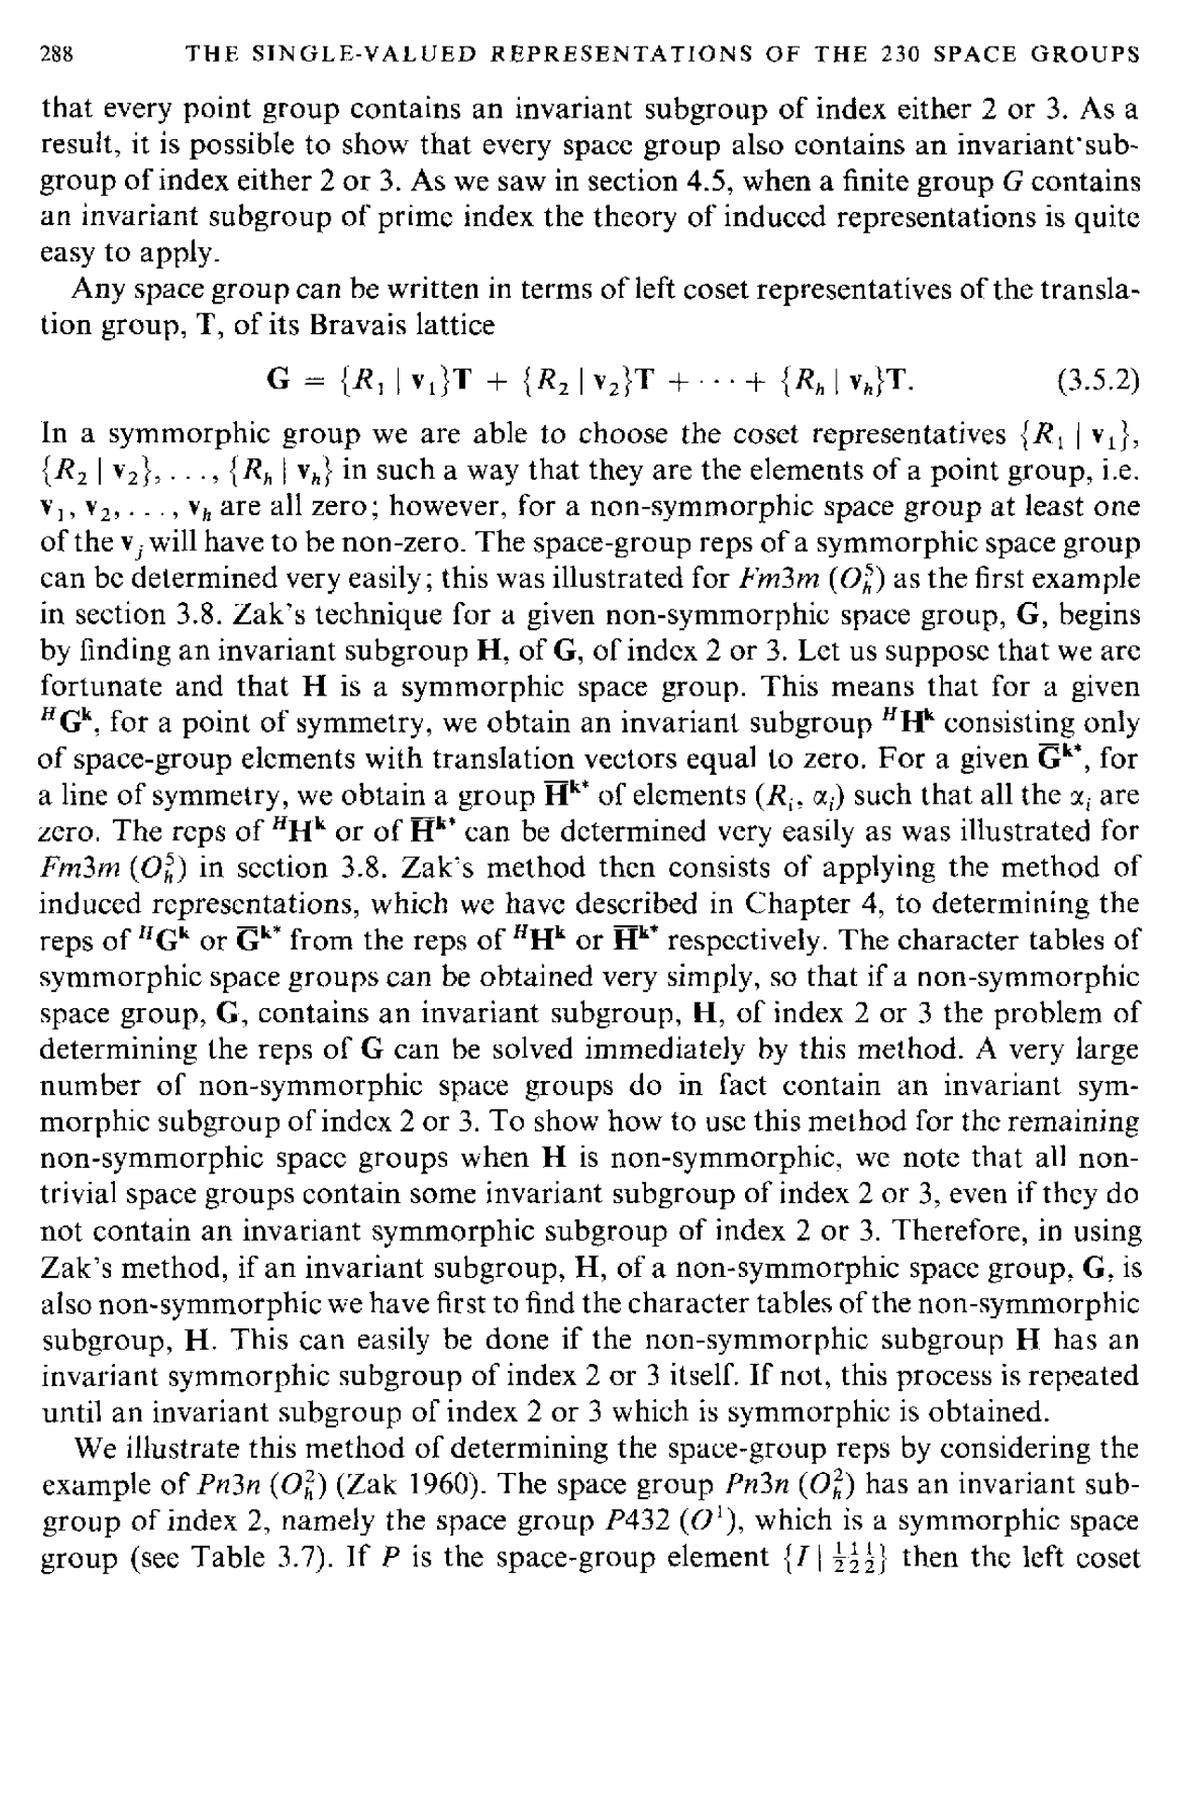
\includegraphics[width=0.86\textwidth]{c5_52_p301.jpg}
\caption*{表 5.3（续）、表 5.4 与表 5.5（原书第 288 页扫描）。}
\end{figure}
\begin{figure}[H]
\centering
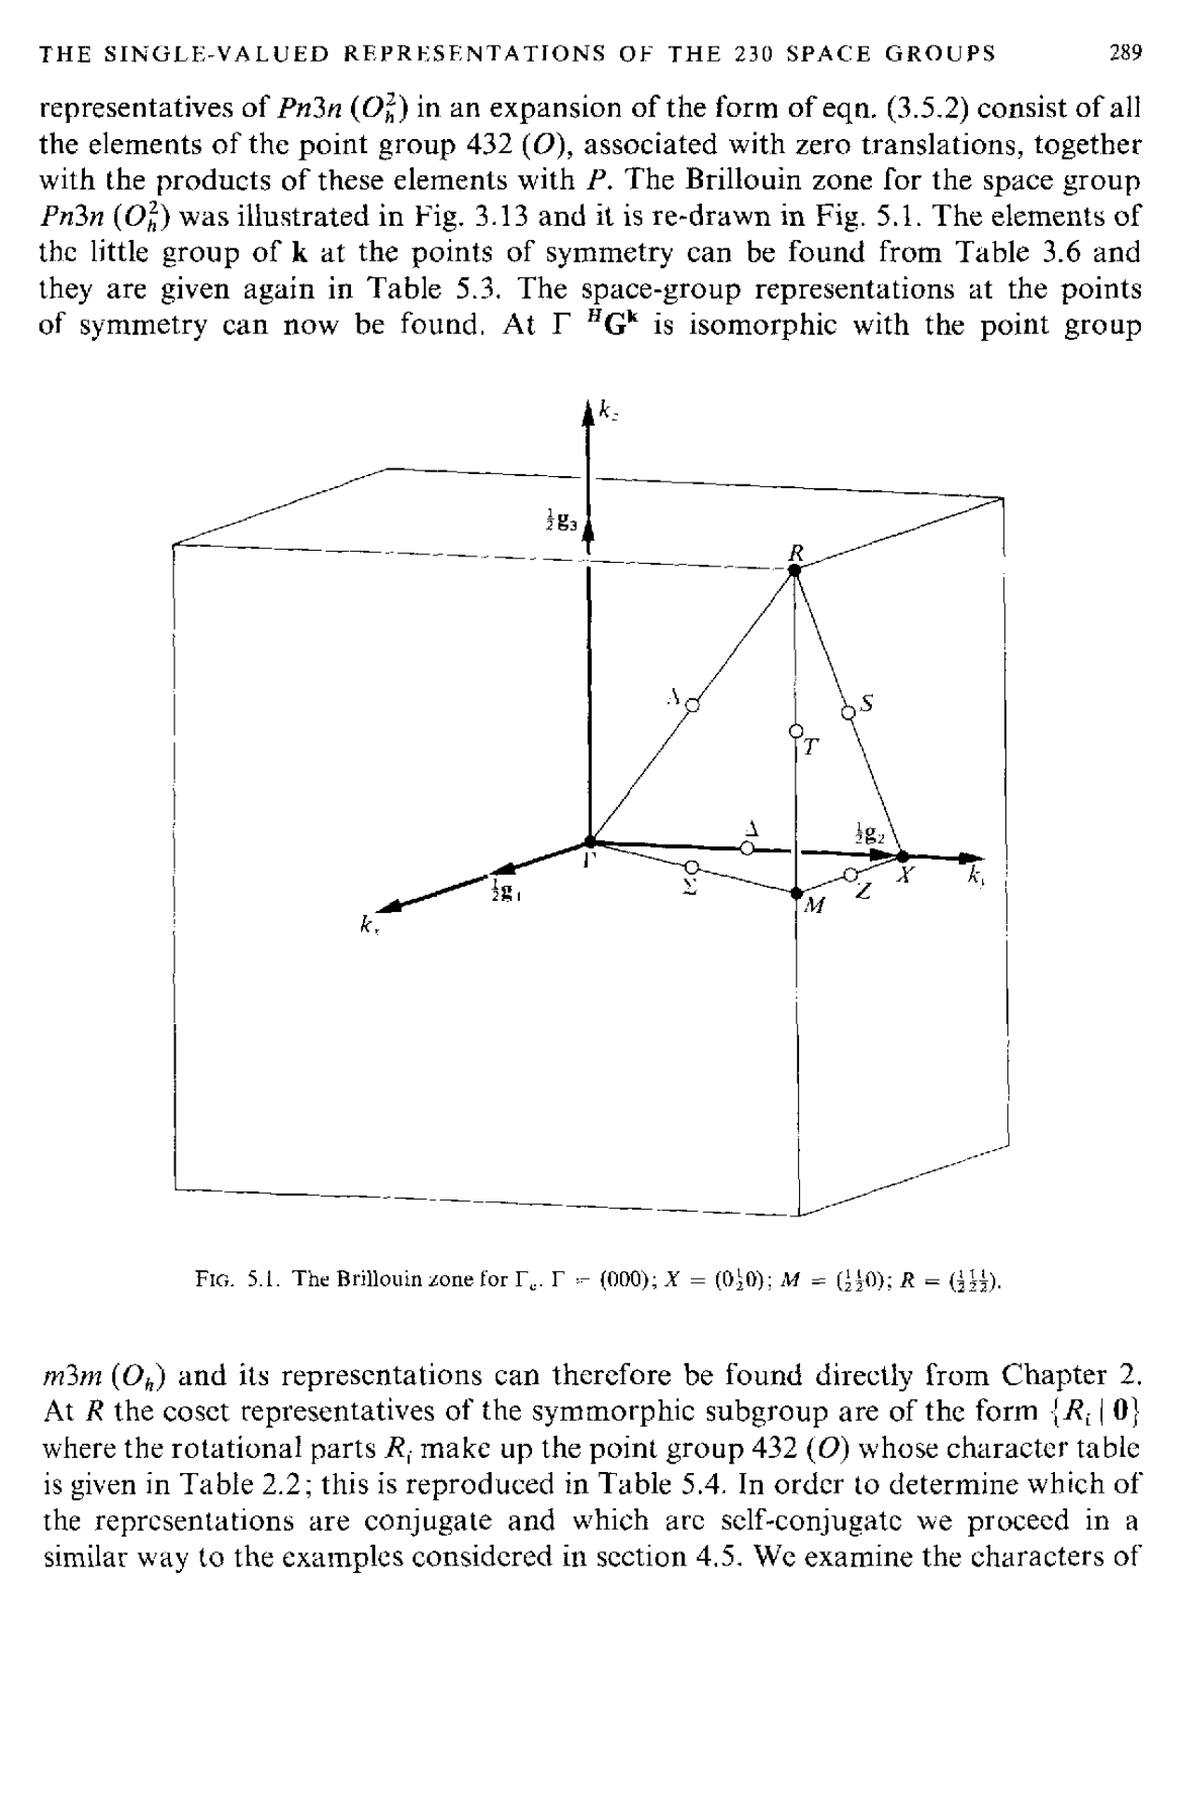
\includegraphics[width=0.86\textwidth]{c5_52_p302.jpg}
\caption*{表 5.5（续）与表 5.6（原书第 289 页扫描）。}
\end{figure}

\begin{figure}[H]
\centering
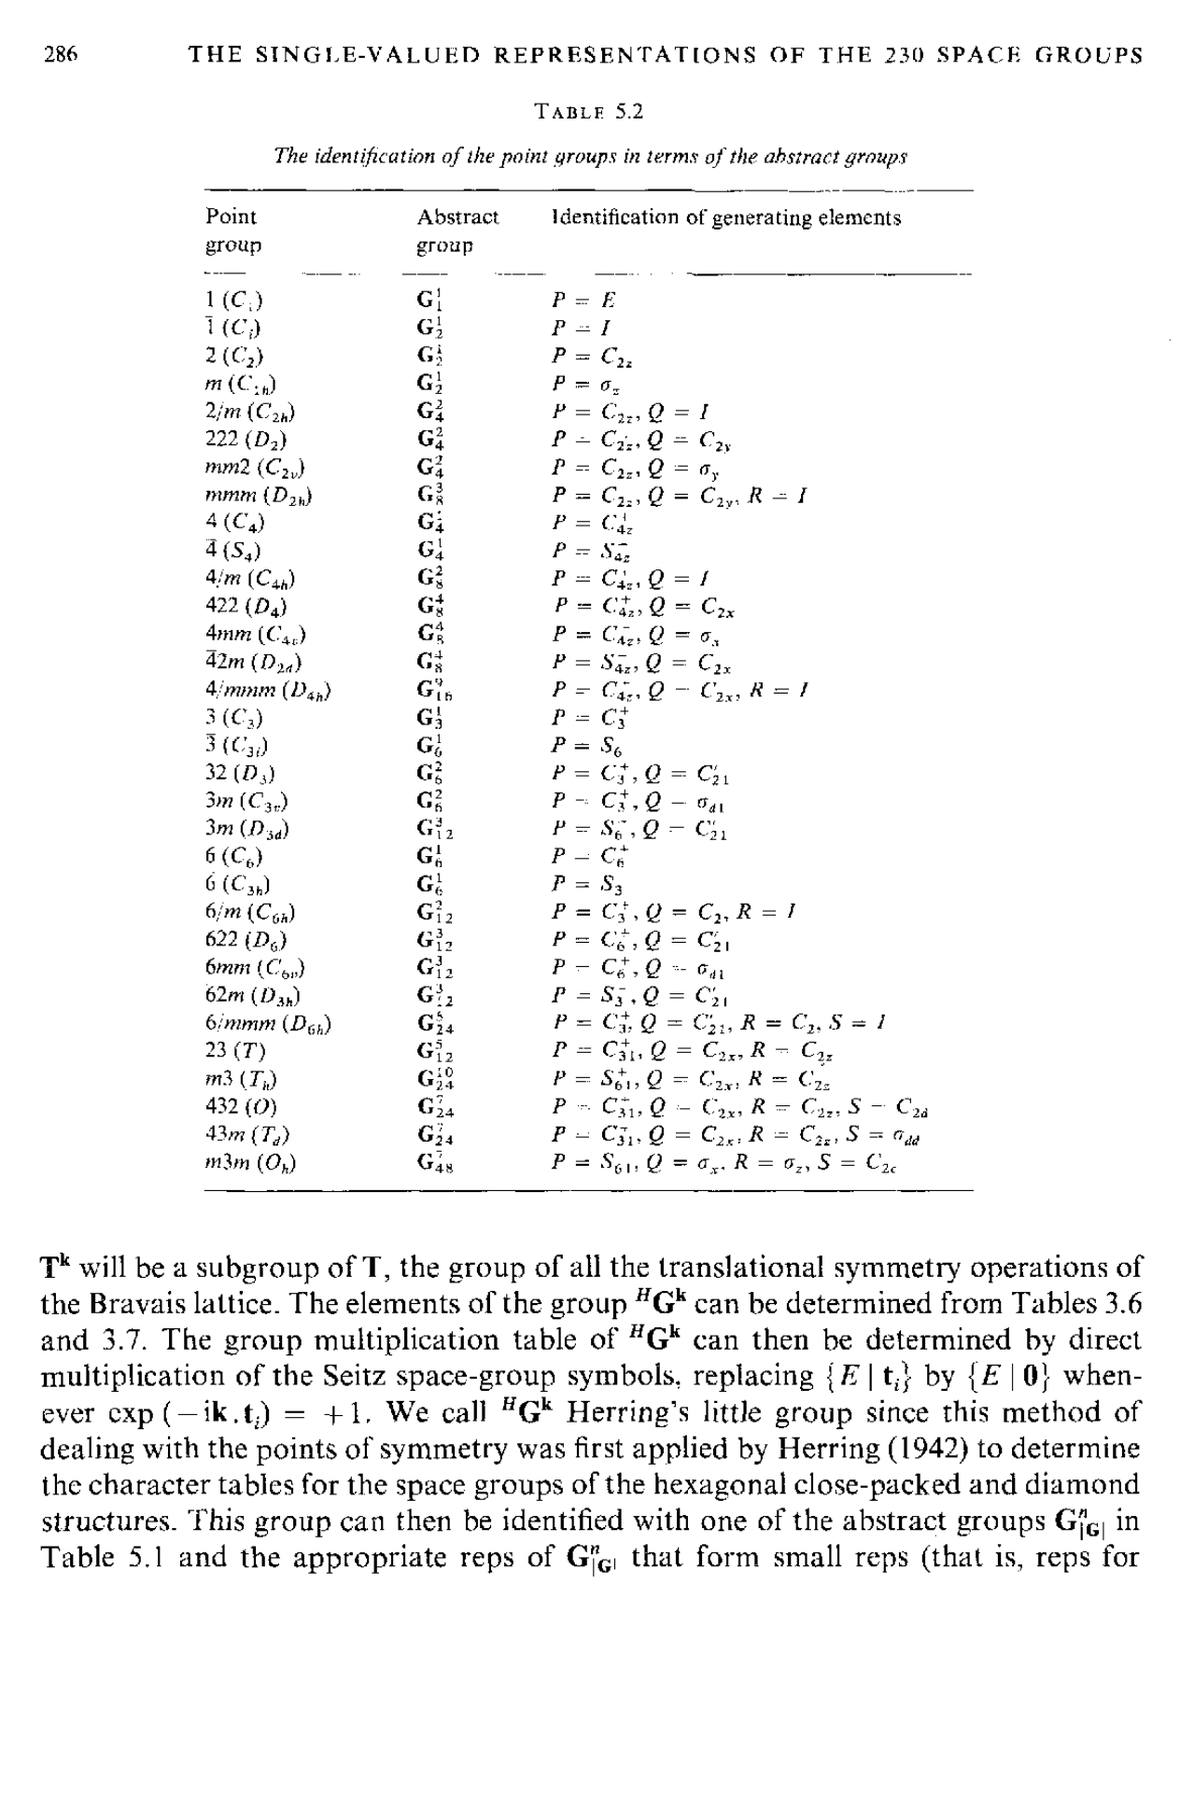
\includegraphics[width=0.86\textwidth]{c5_52_p299.jpg}
\caption*{原书第 286 页}
\end{figure}
\begin{figure}[H]
\centering
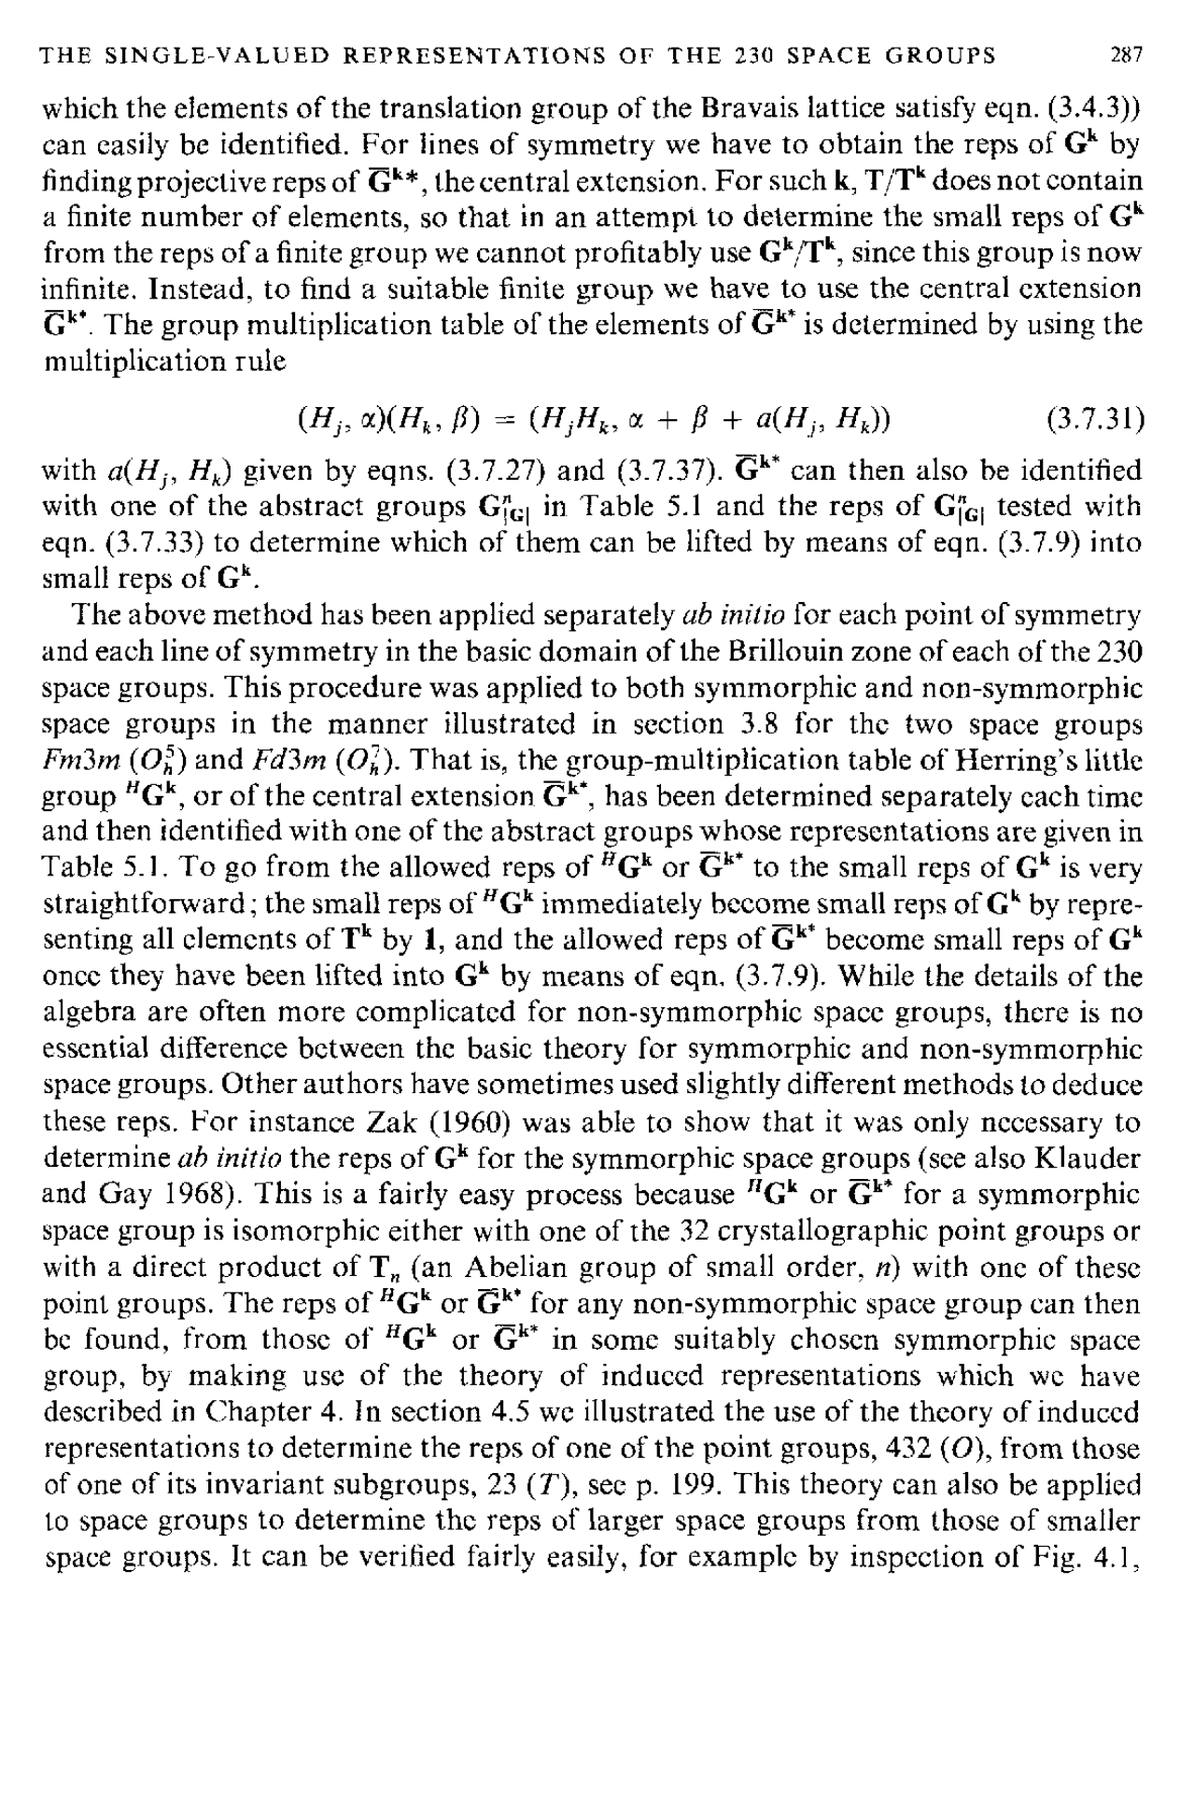
\includegraphics[width=0.86\textwidth]{c5_52_p300.jpg}
\caption*{原书第 287 页}
\end{figure}
\begin{figure}[H]
\centering
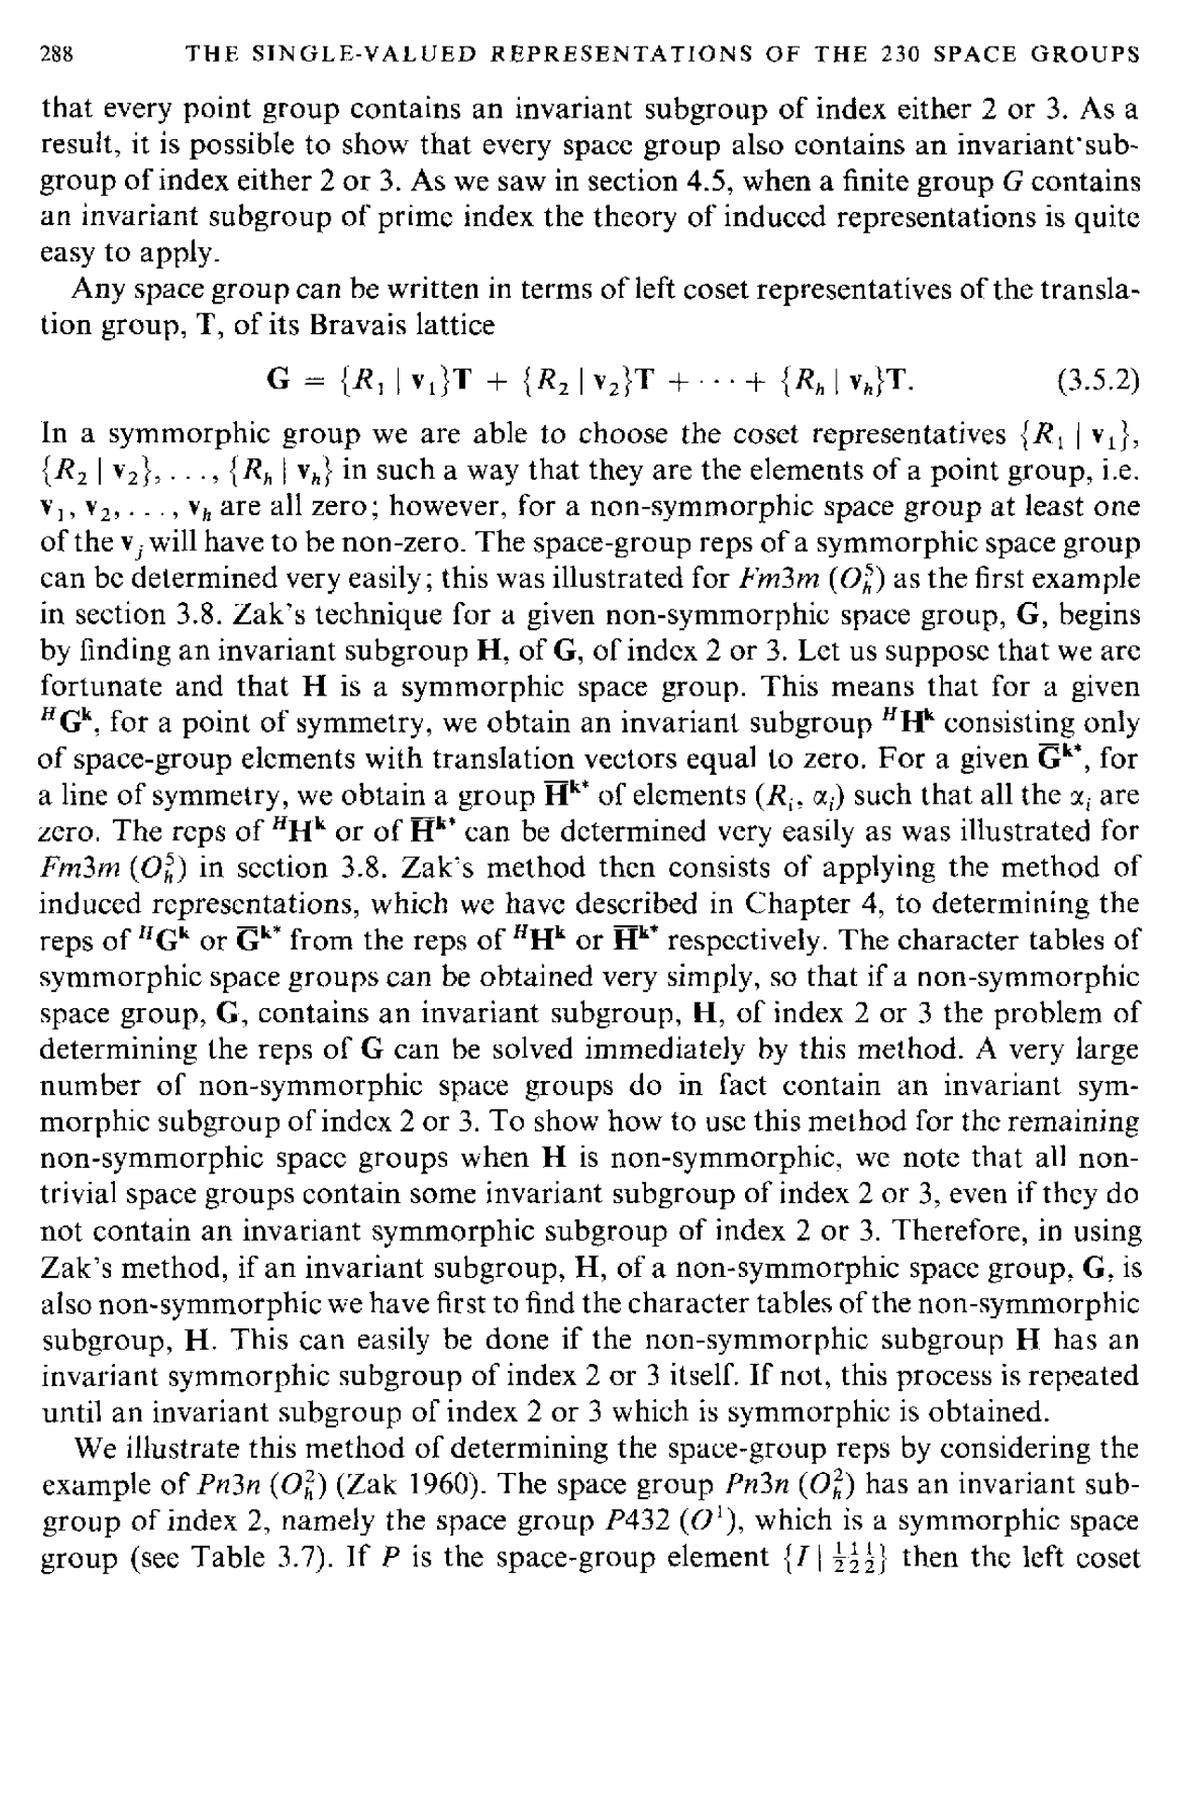
\includegraphics[width=0.86\textwidth]{c5_52_p301.jpg}
\caption*{原书第 288 页}
\end{figure}
\begin{figure}[H]
\centering
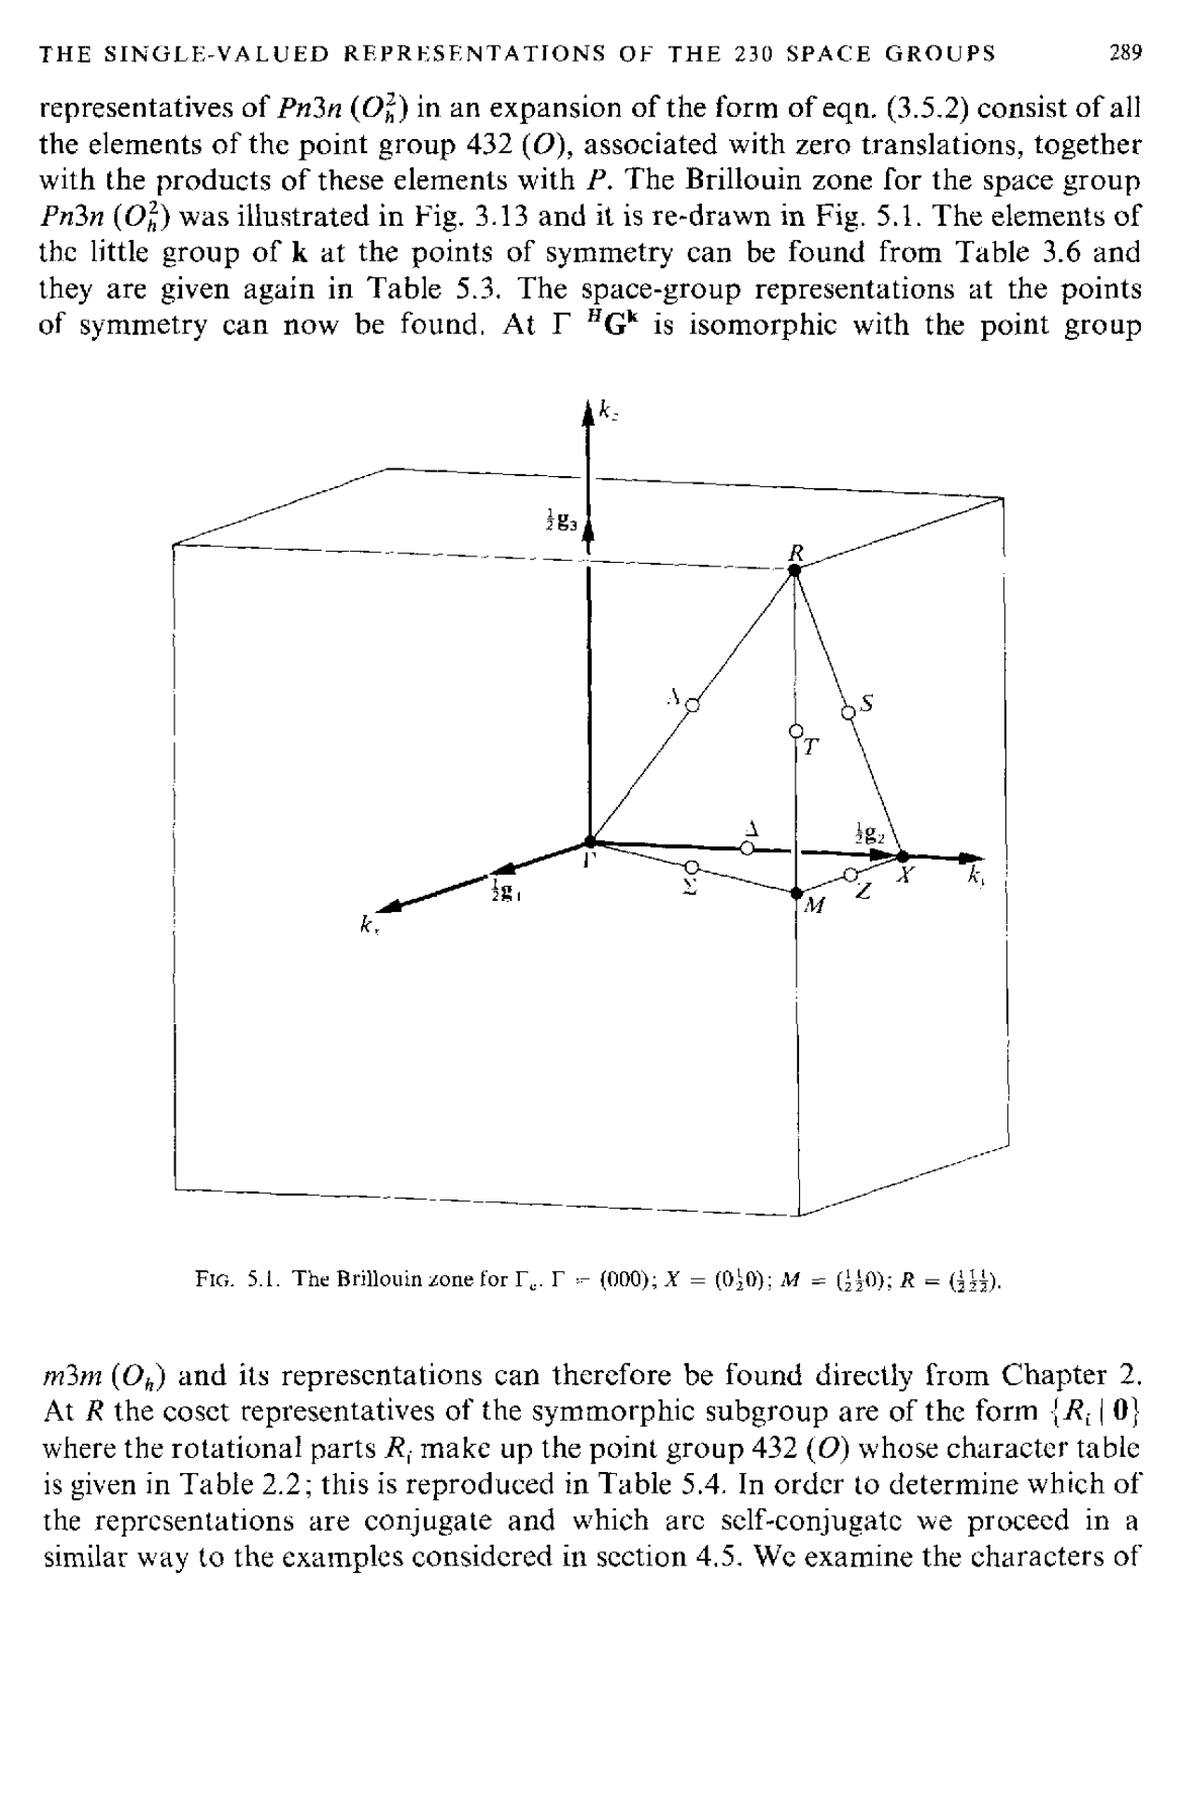
\includegraphics[width=0.86\textwidth]{c5_52_p302.jpg}
\caption*{原书第 289 页}
\end{figure}
\begin{figure}[H]
\centering
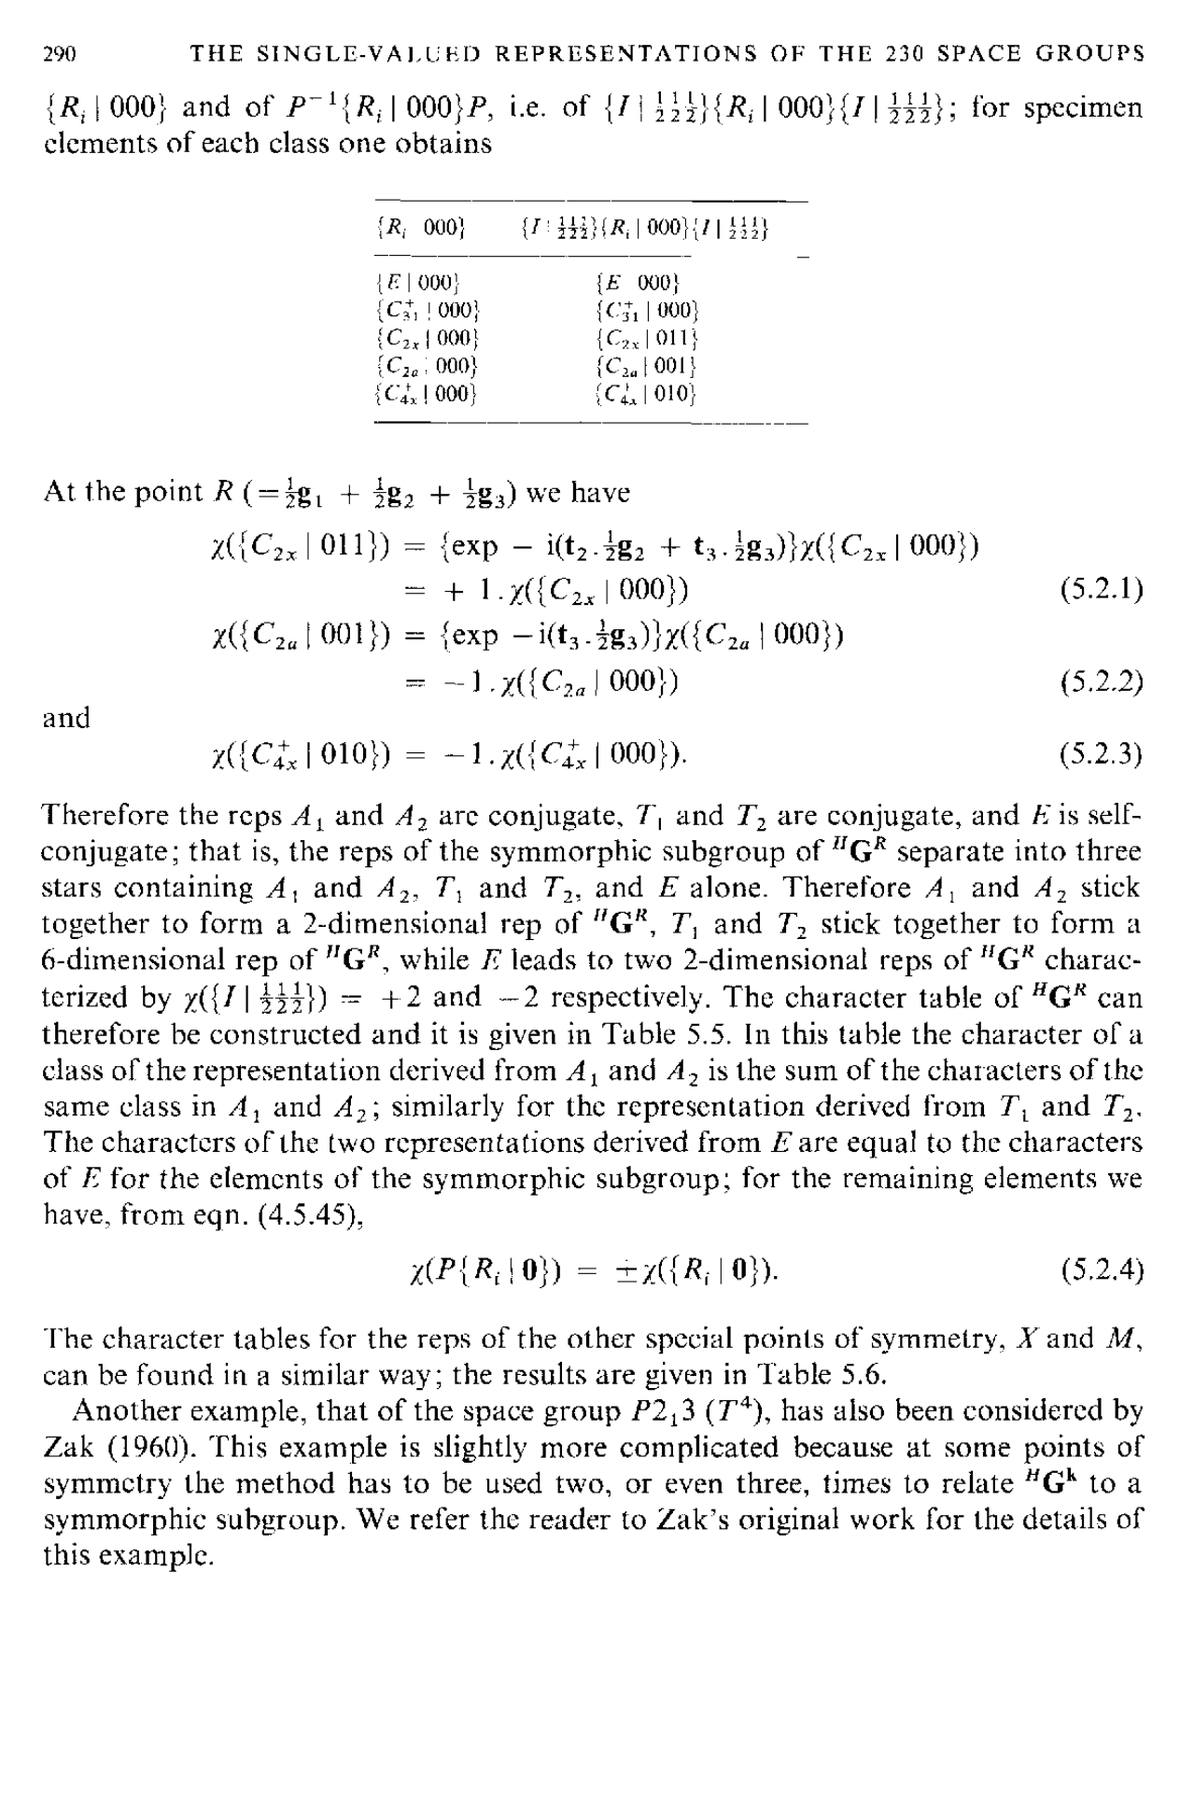
\includegraphics[width=0.86\textwidth]{c5_52_p303.jpg}
\caption*{原书第 290 页}
\end{figure}
\begin{figure}[H]
\centering
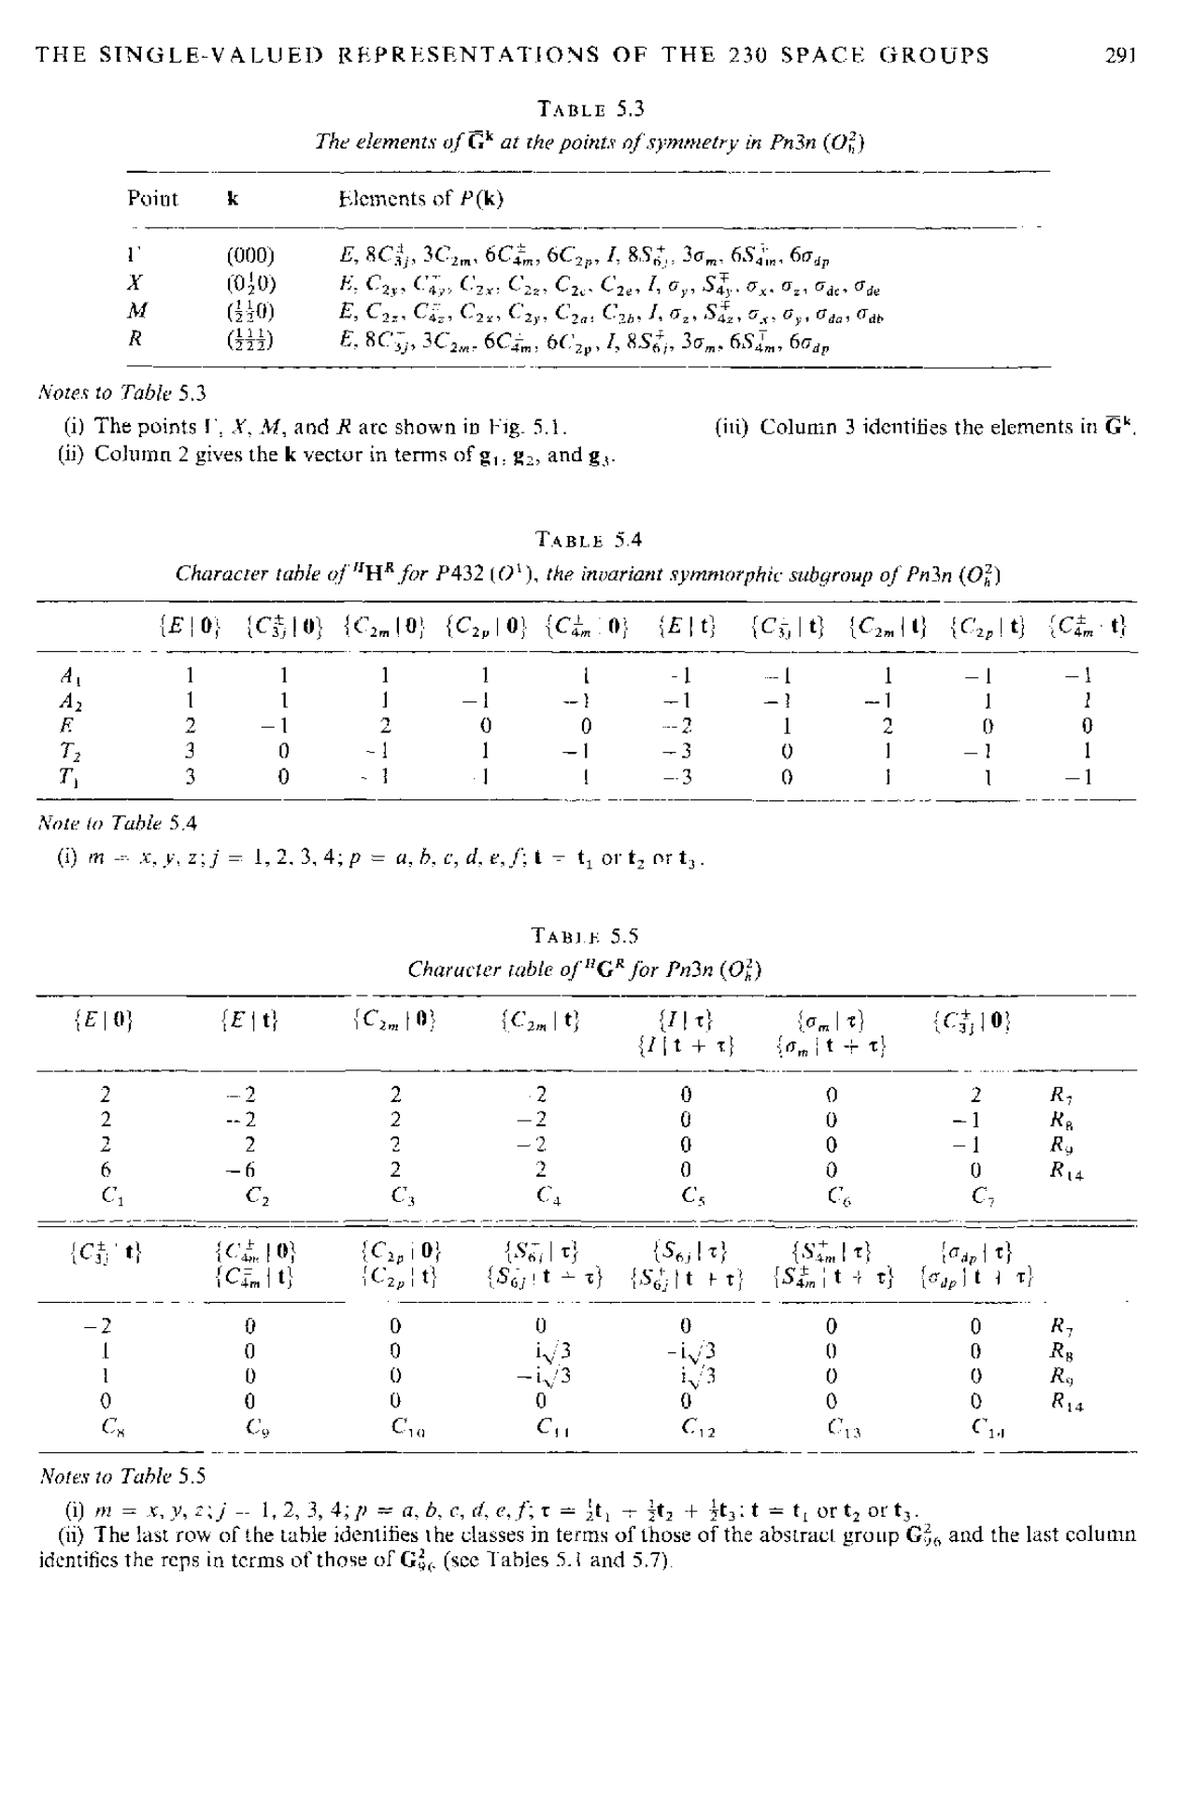
\includegraphics[width=0.86\textwidth]{c5_52_p304.jpg}
\caption*{原书第 291 页}
\end{figure}
\begin{figure}[H]
\centering
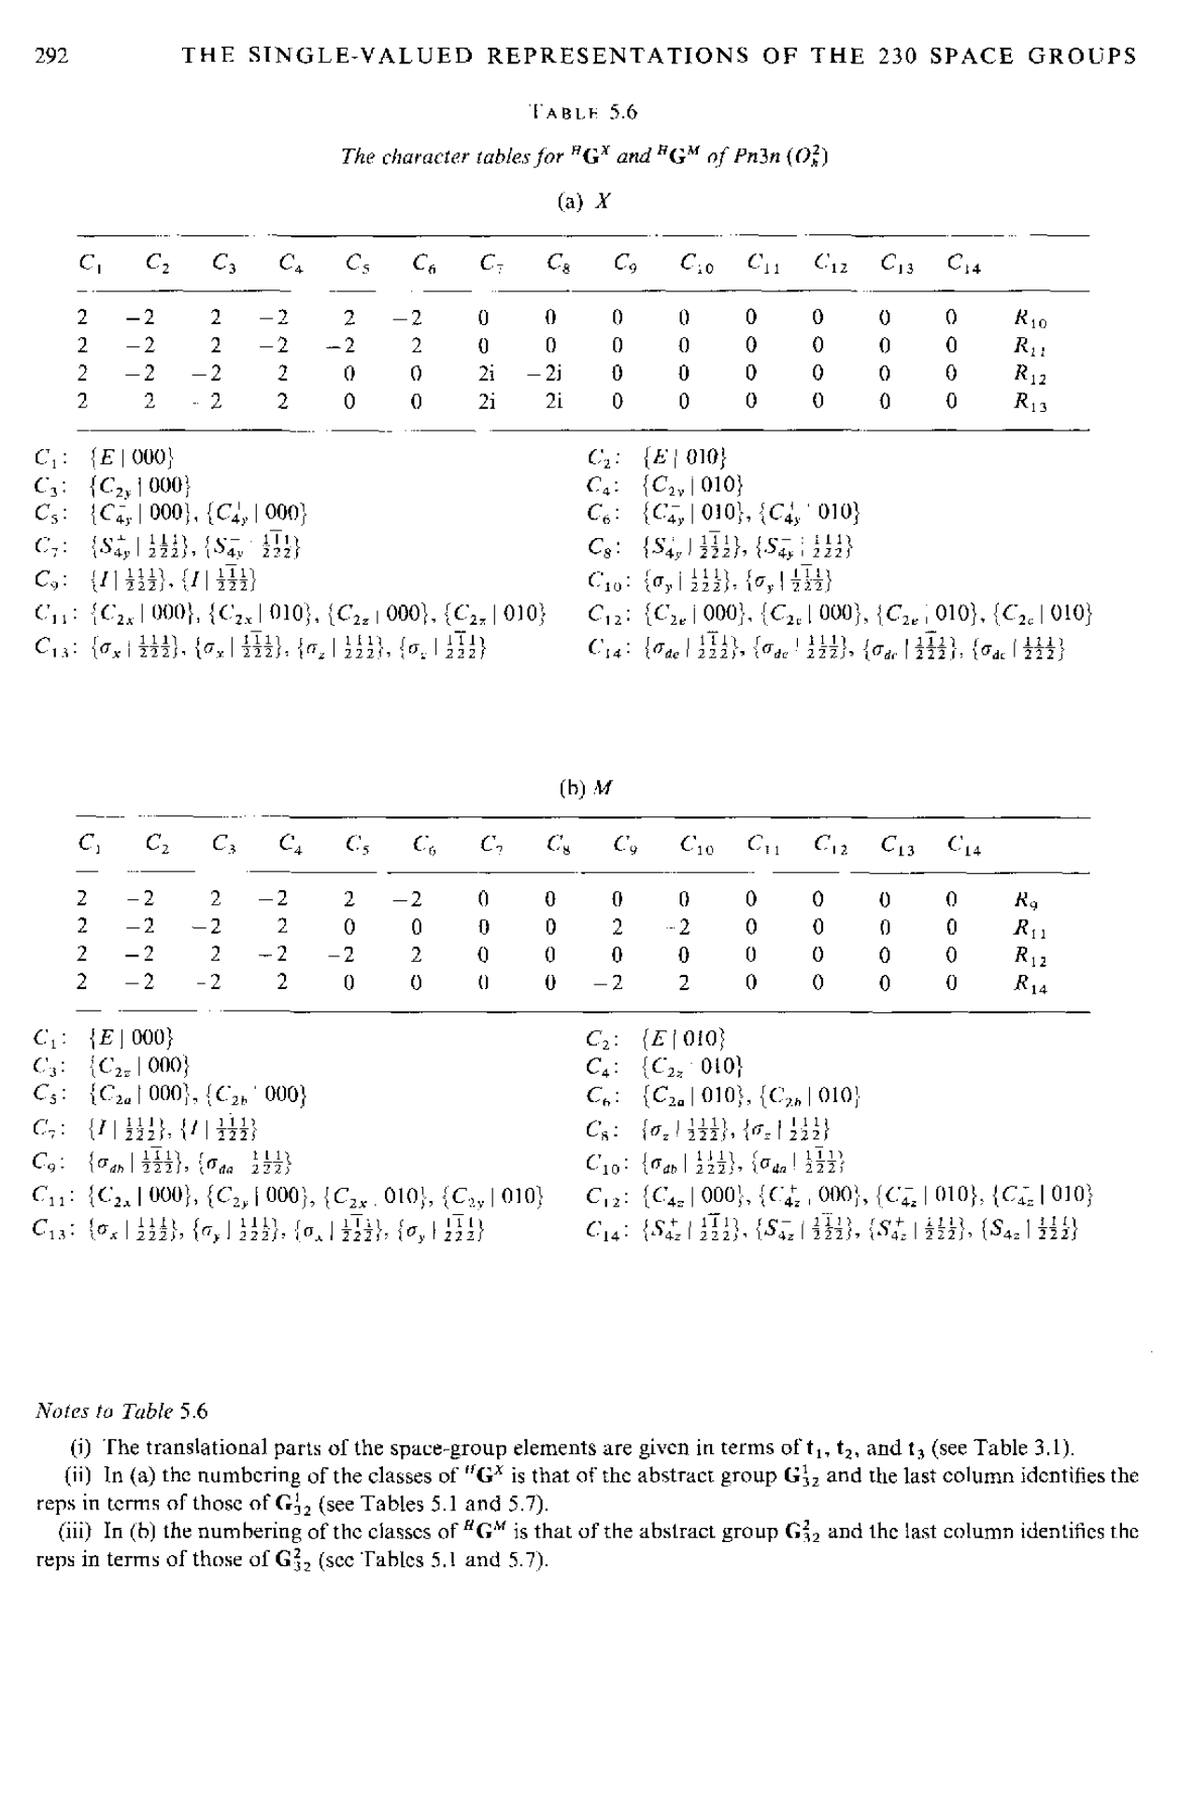
\includegraphics[width=0.86\textwidth]{c5_52_p305.jpg}
\caption*{原书第 292 页}
\end{figure}
\begin{figure}[H]
\centering
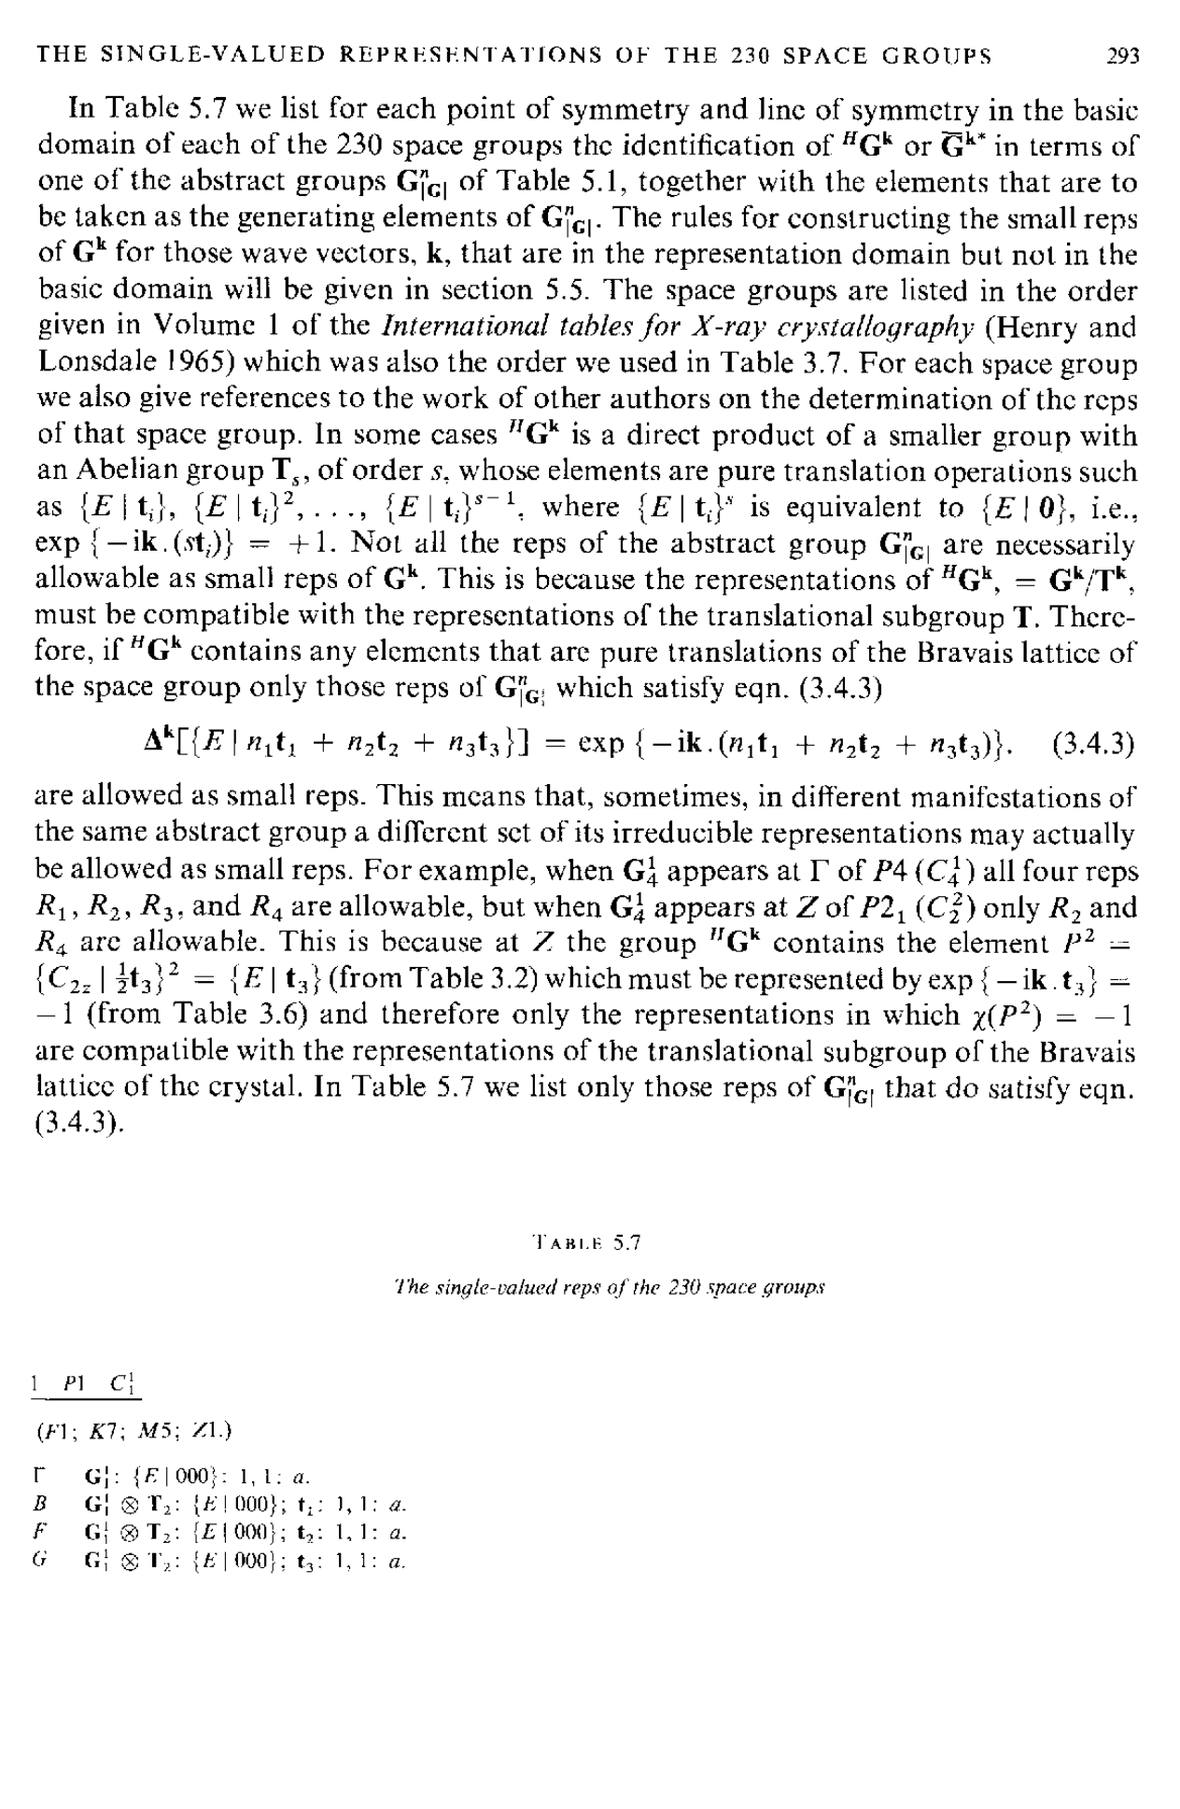
\includegraphics[width=0.86\textwidth]{c5_52_p306.jpg}
\caption*{原书第 293 页}
\end{figure}
\begin{figure}[H]
\centering
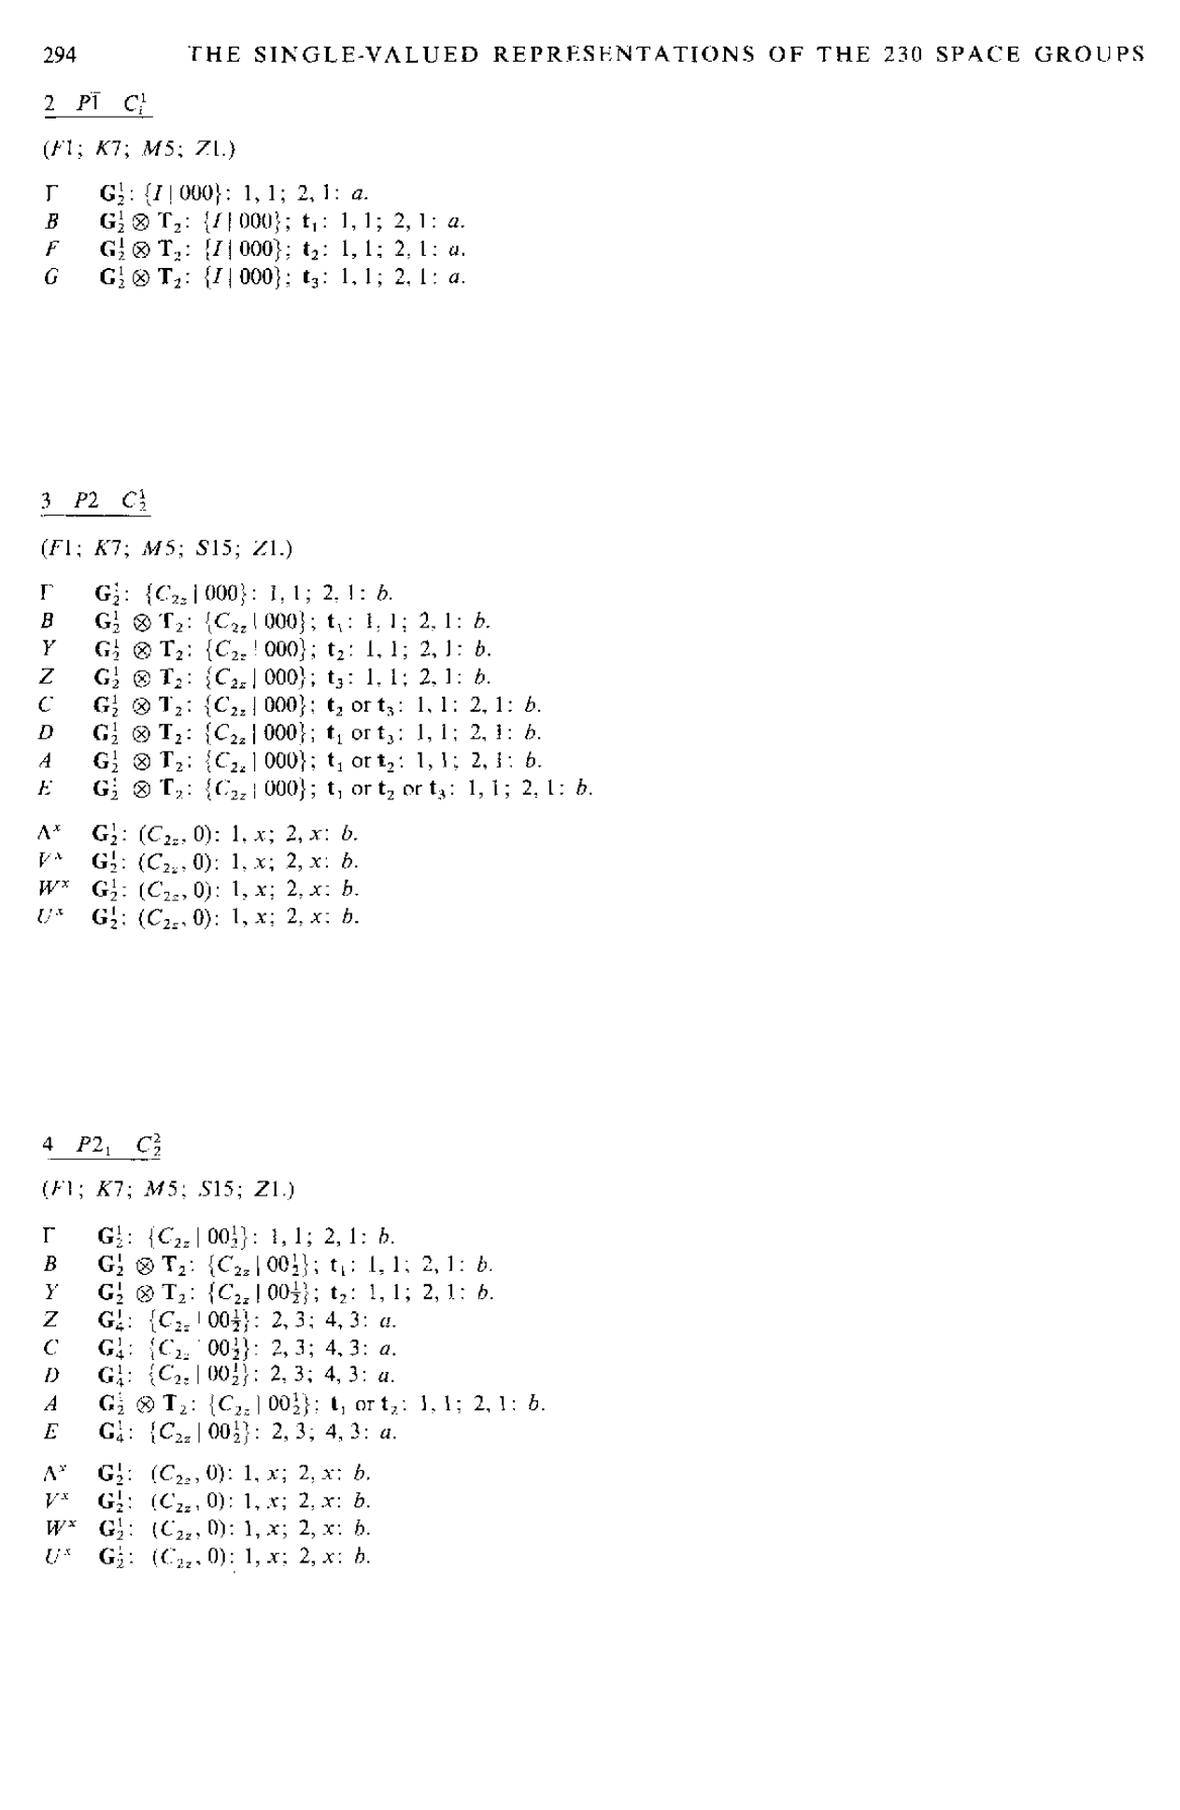
\includegraphics[width=0.86\textwidth]{c5_52_p307.jpg}
\caption*{原书第 294 页}
\end{figure}
\begin{figure}[H]
\centering
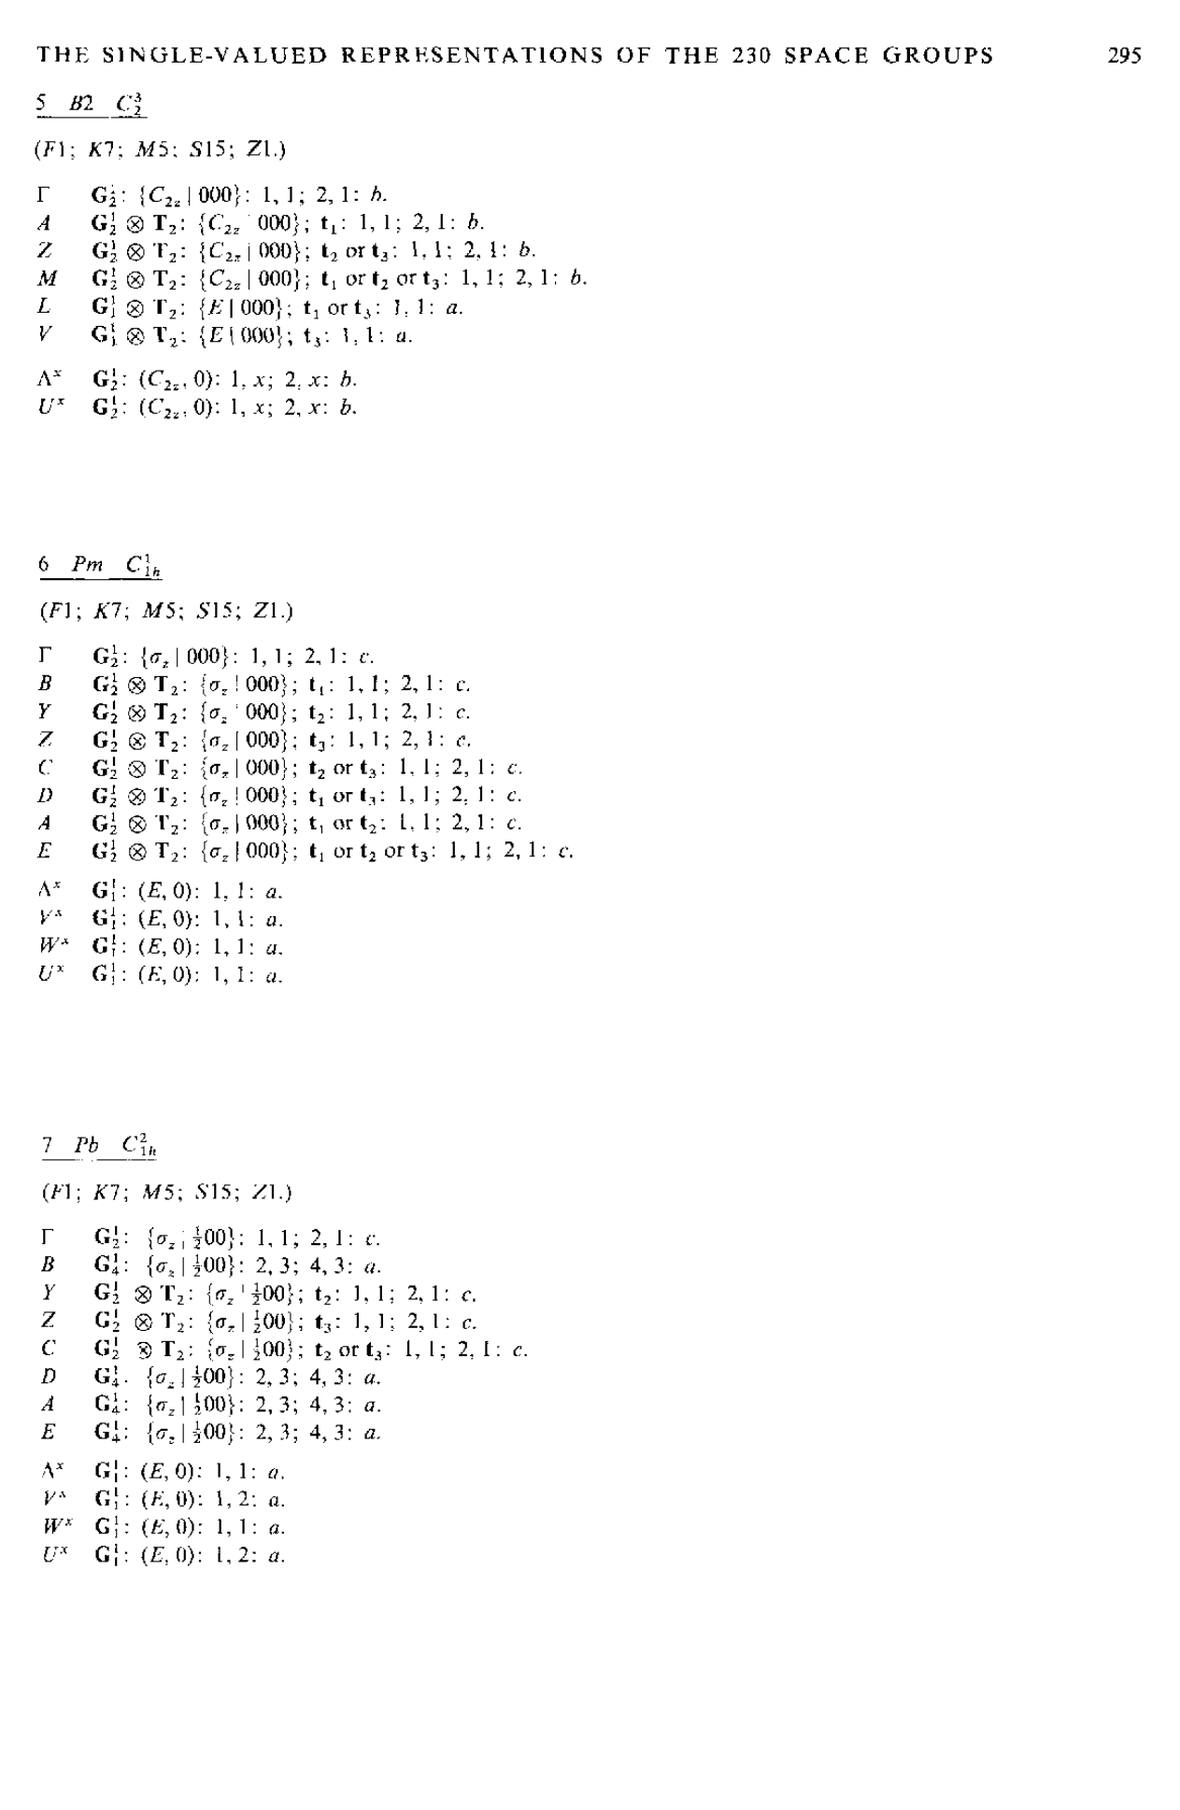
\includegraphics[width=0.86\textwidth]{c5_52_p308.jpg}
\caption*{原书第 295 页}
\end{figure}
\begin{figure}[H]
\centering
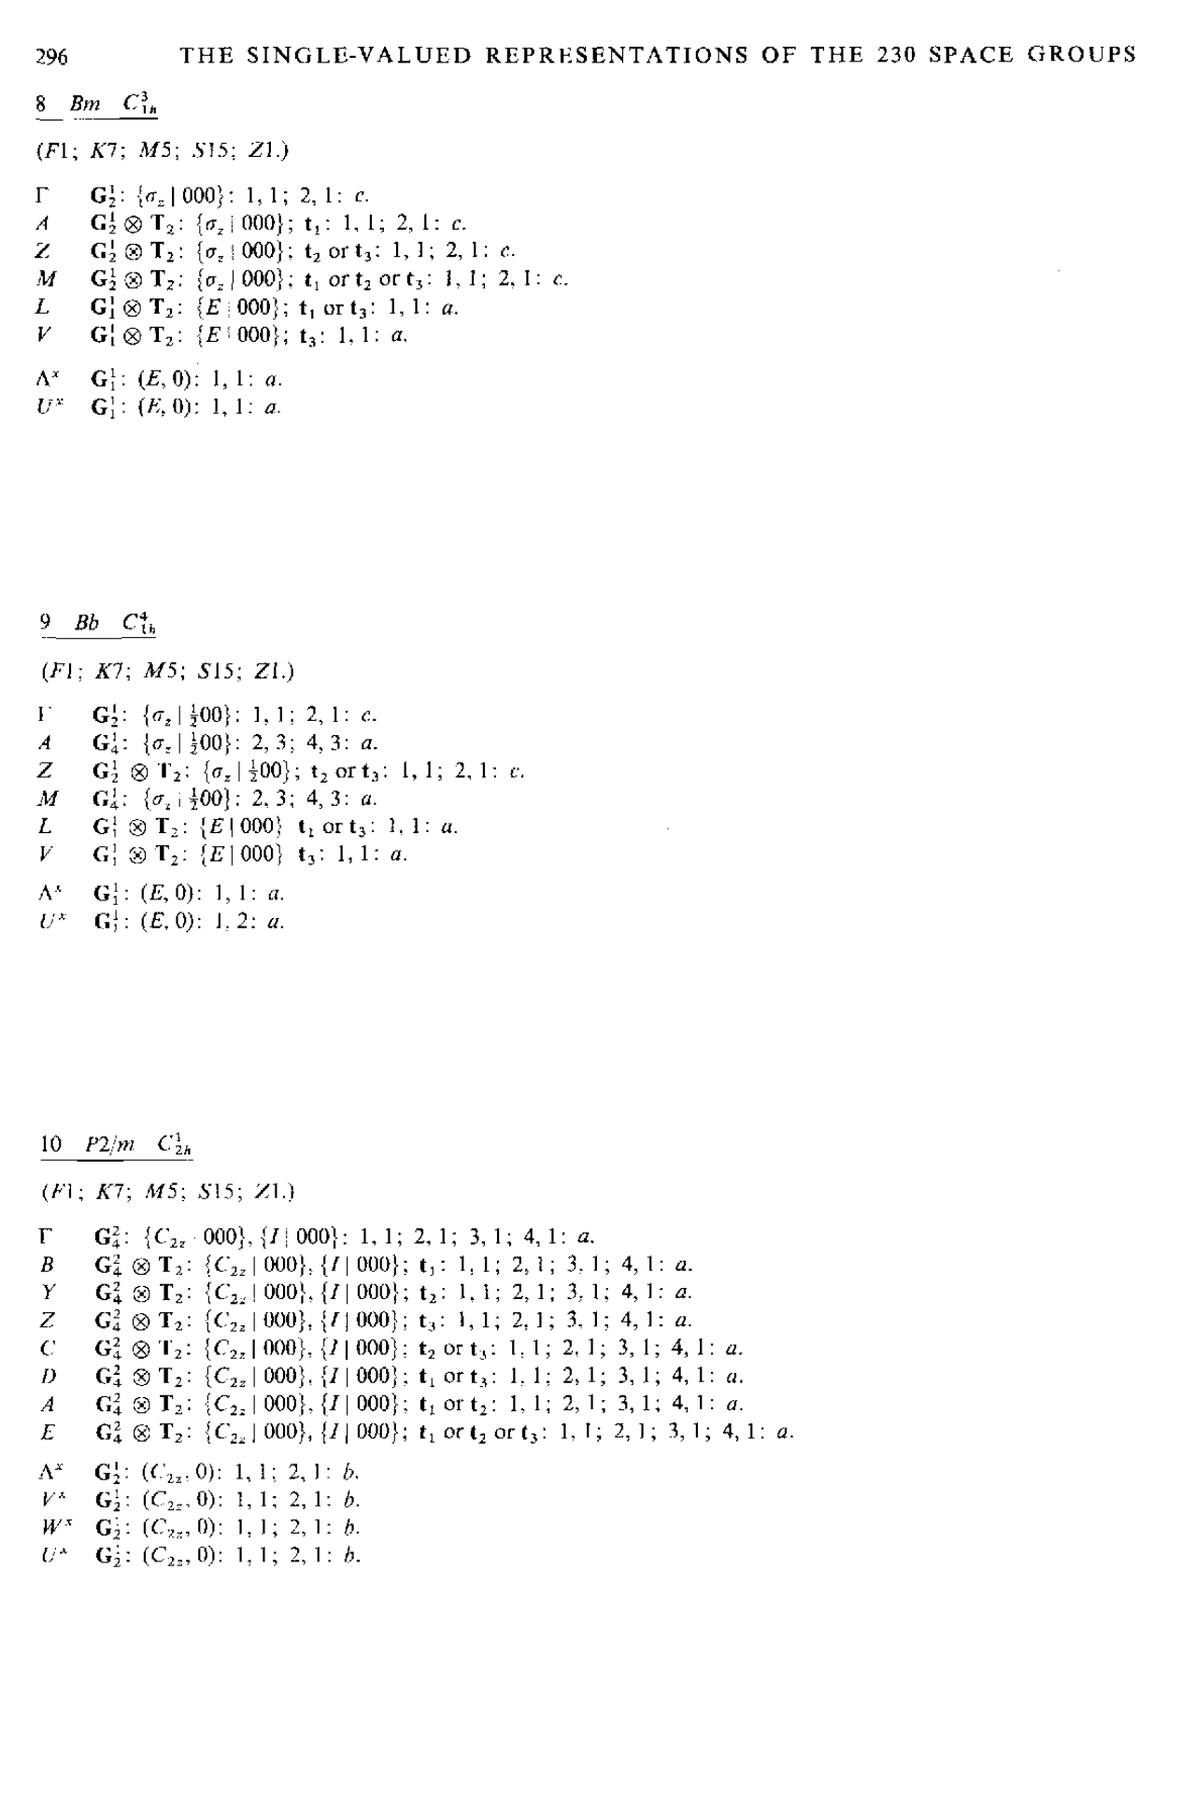
\includegraphics[width=0.86\textwidth]{c5_52_p309.jpg}
\caption*{原书第 296 页}
\end{figure}
\begin{figure}[H]
\centering
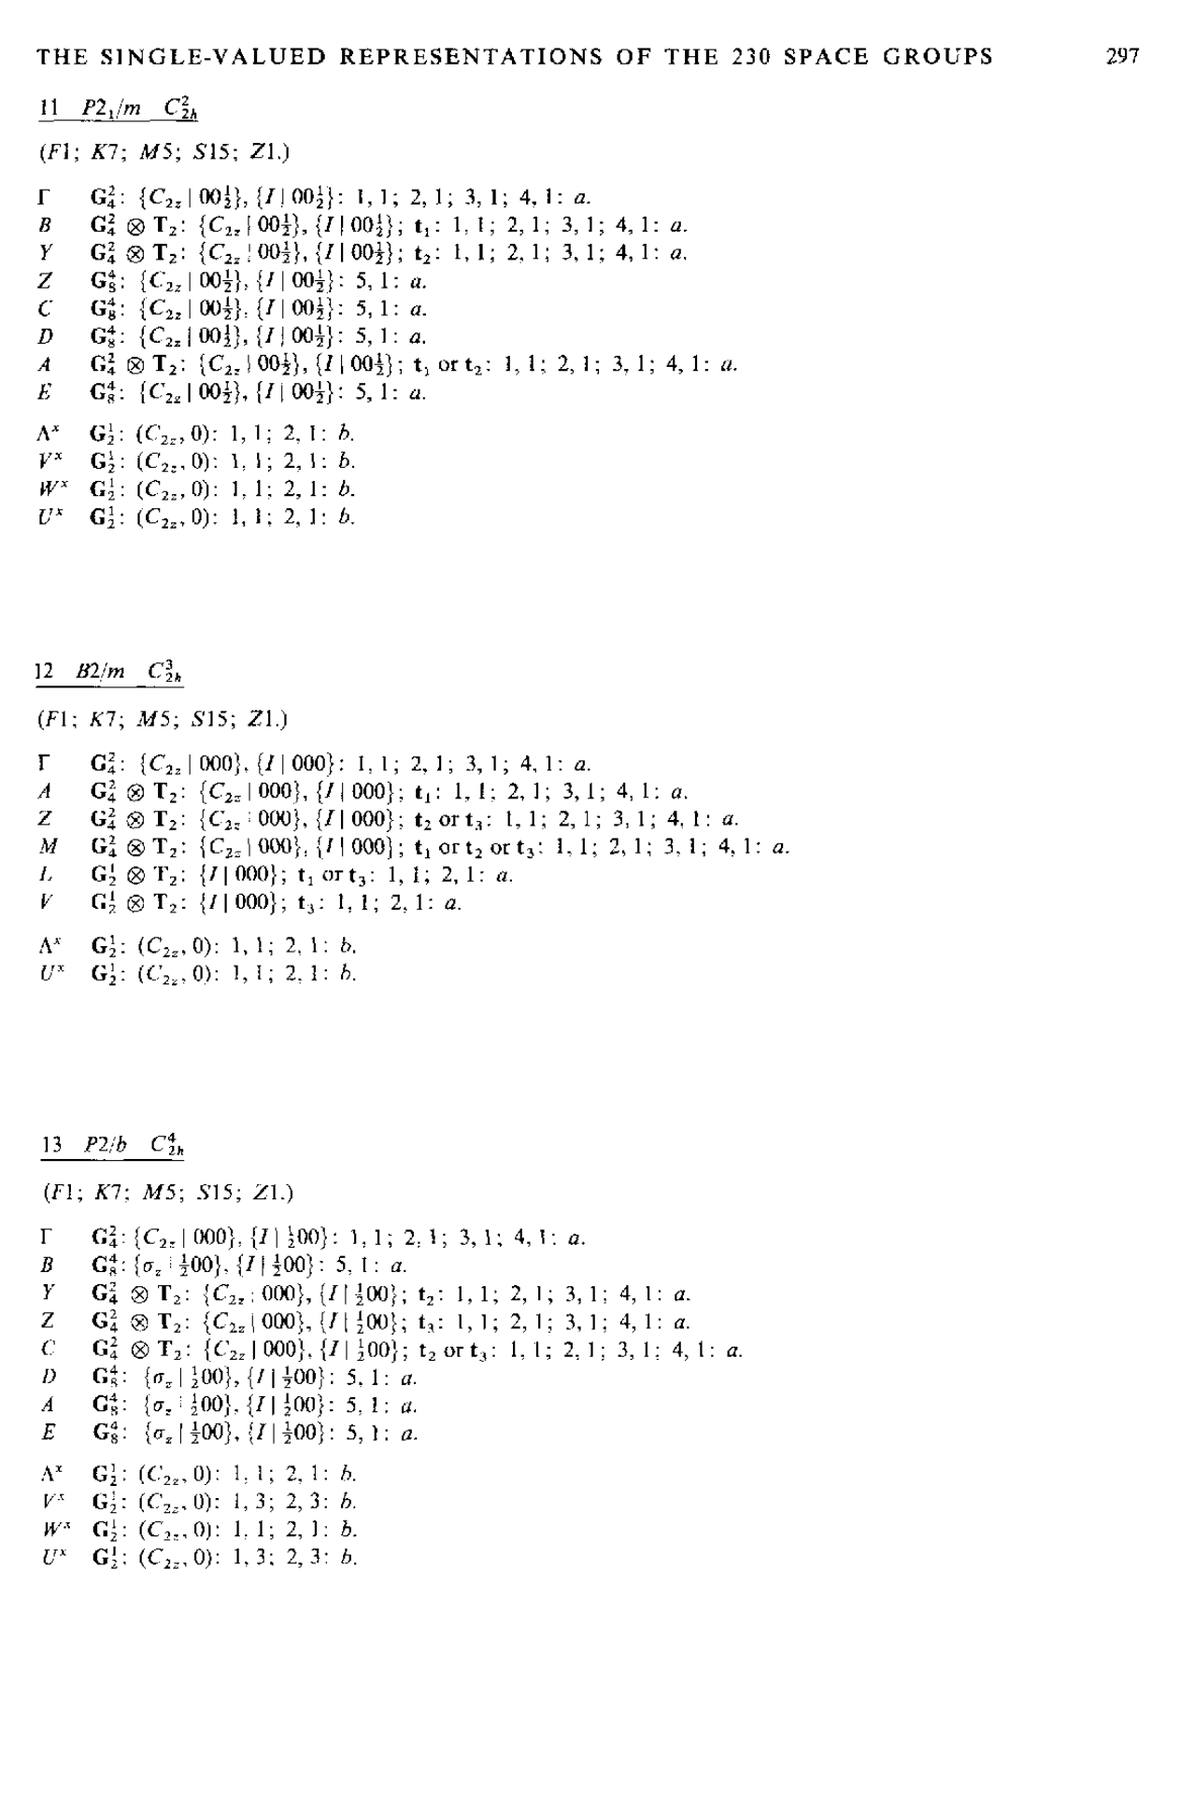
\includegraphics[width=0.86\textwidth]{c5_52_p310.jpg}
\caption*{原书第 297 页}
\end{figure}
\begin{figure}[H]
\centering
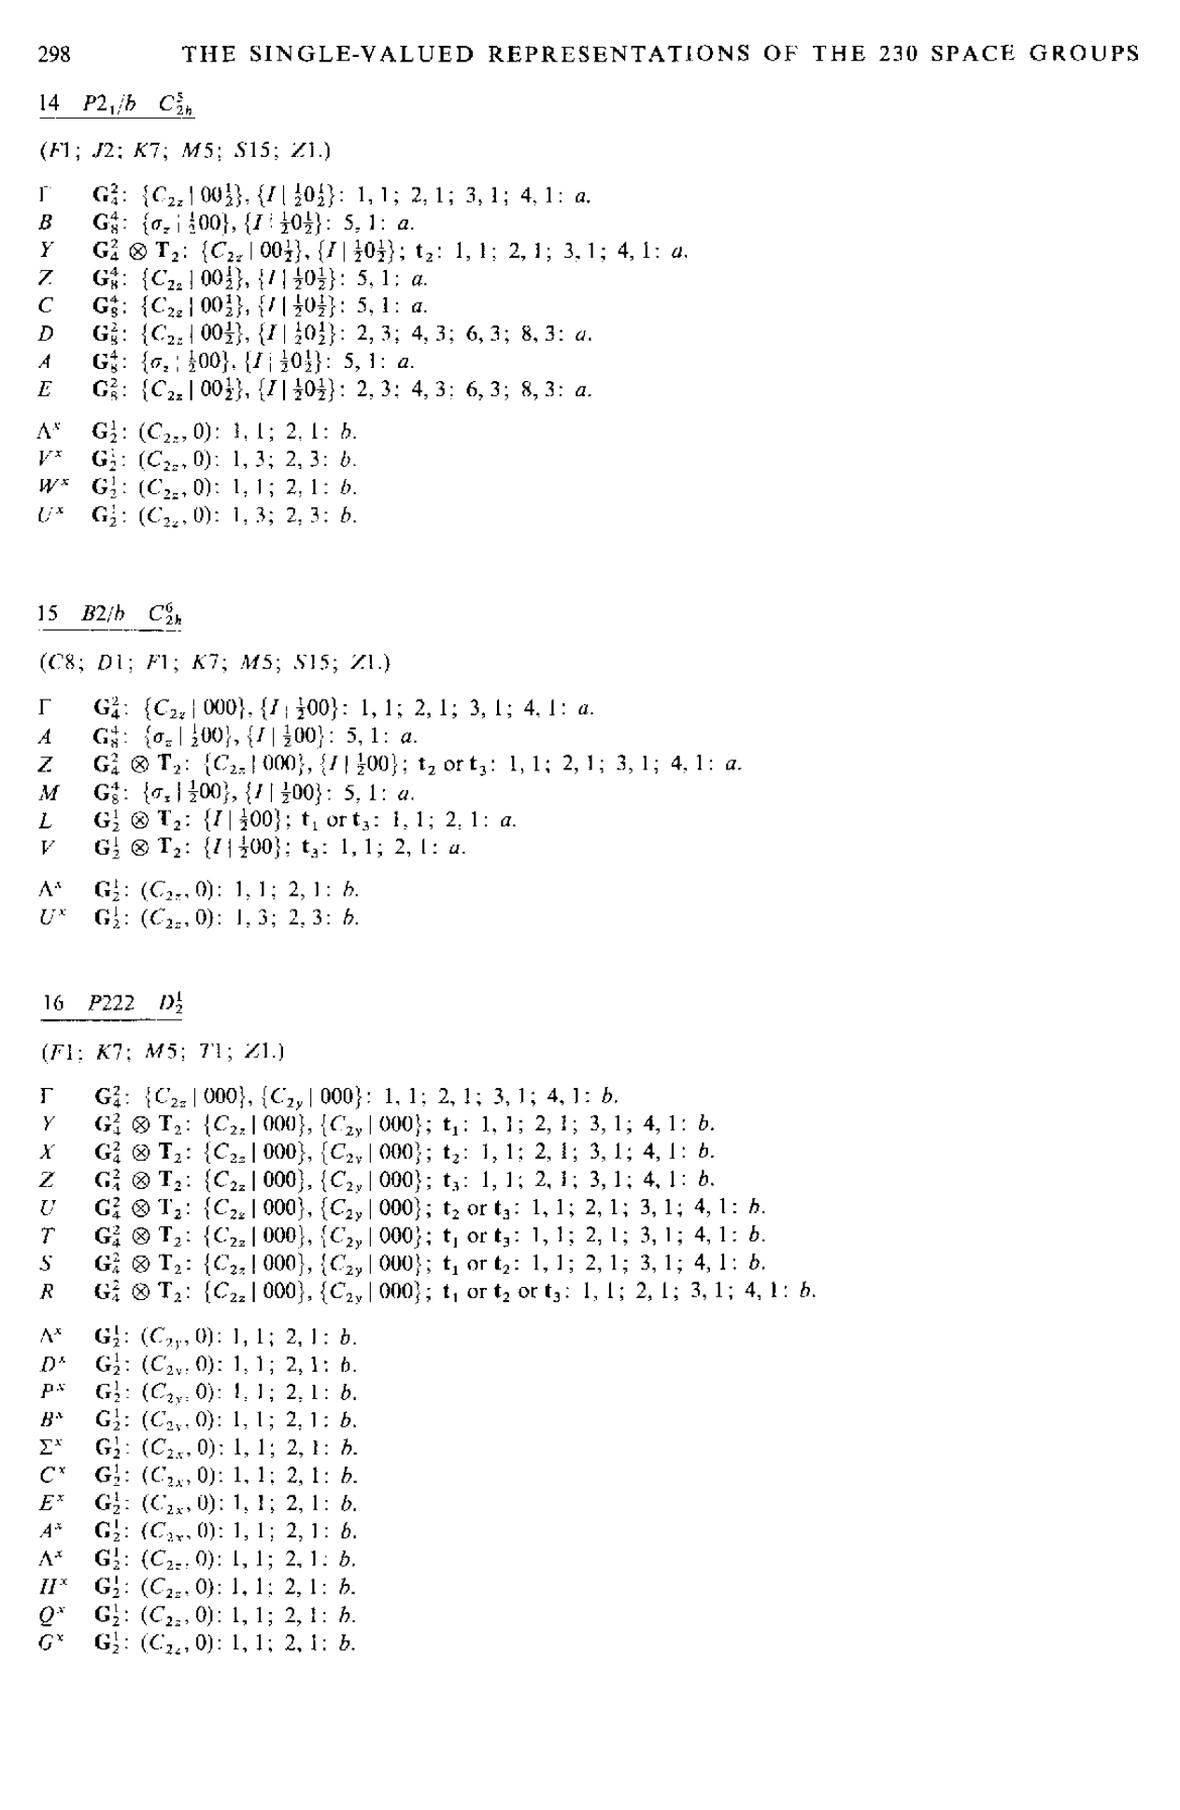
\includegraphics[width=0.86\textwidth]{c5_52_p311.jpg}
\caption*{原书第 298 页}
\end{figure}
\begin{figure}[H]
\centering
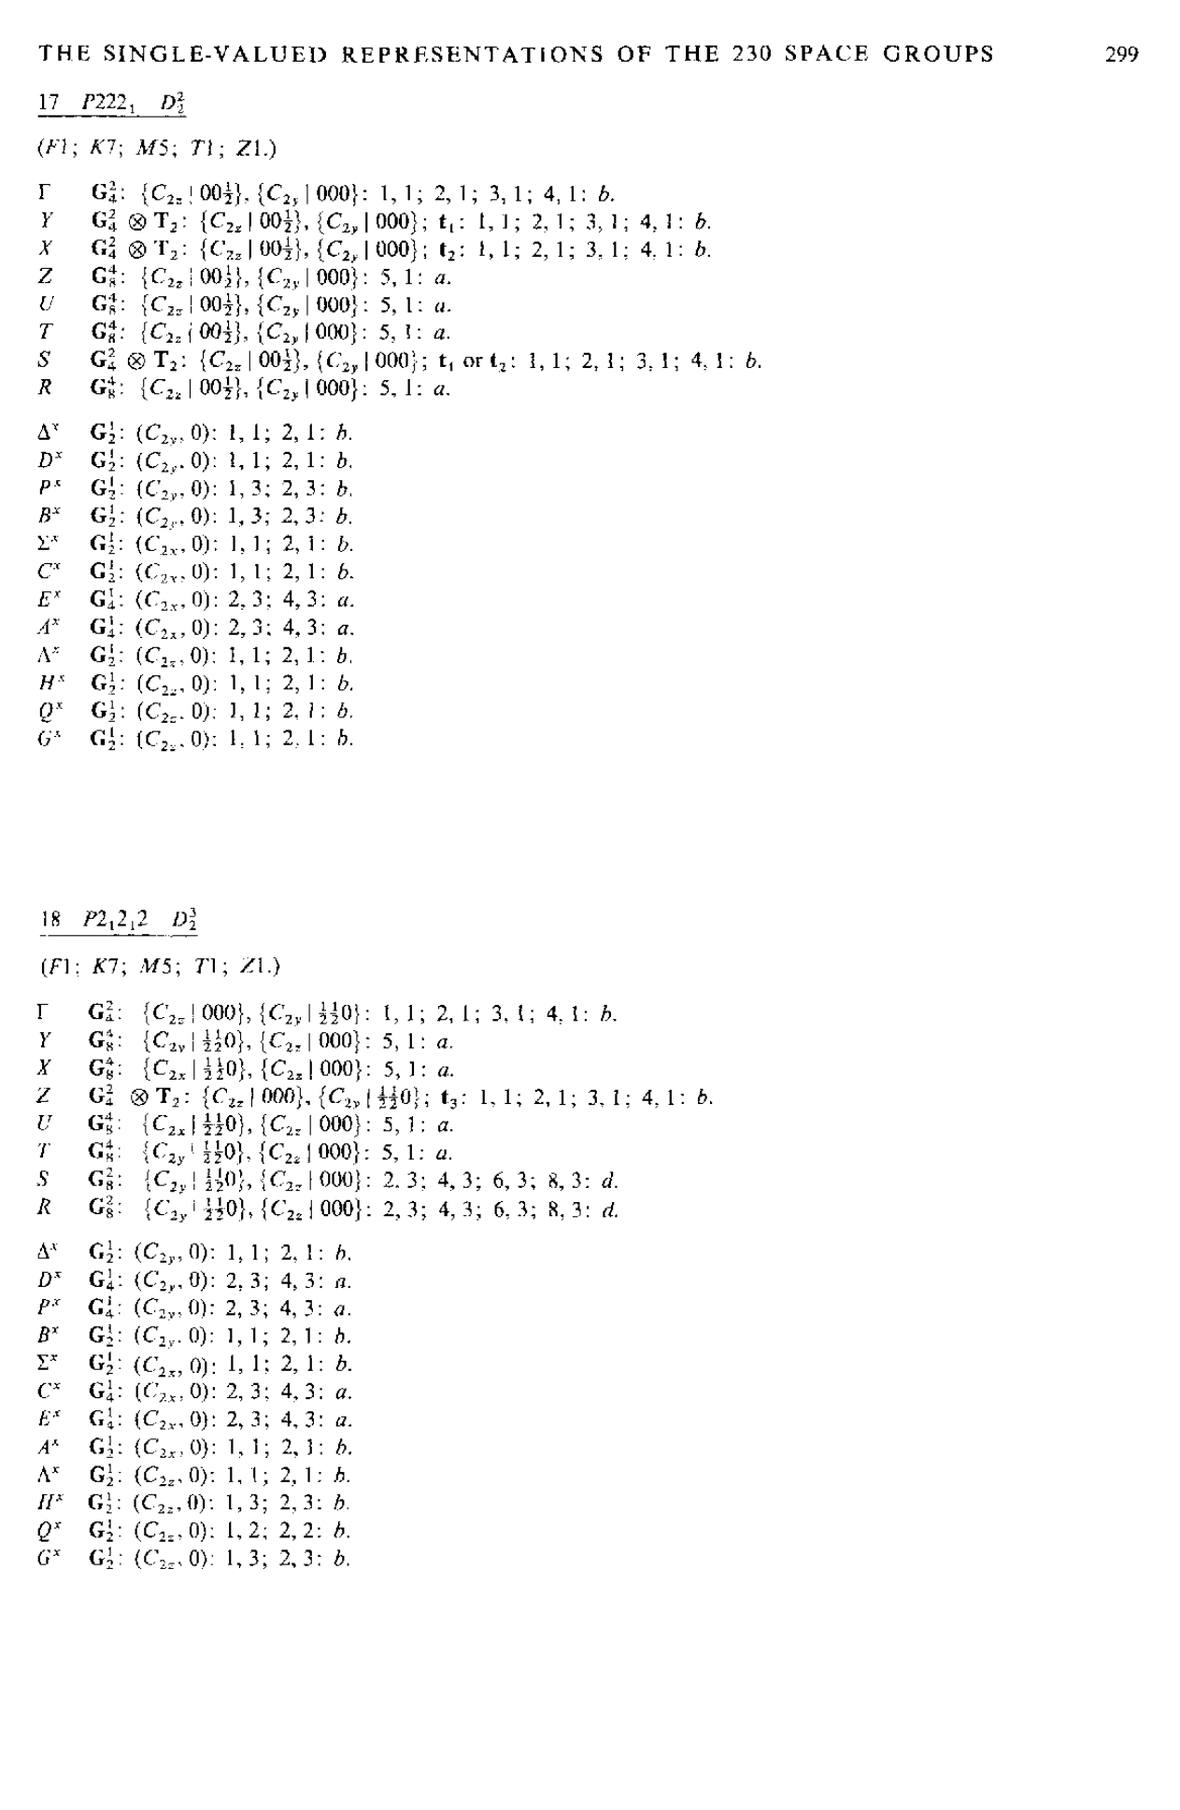
\includegraphics[width=0.86\textwidth]{c5_52_p312.jpg}
\caption*{原书第 299 页}
\end{figure}
\begin{figure}[H]
\centering
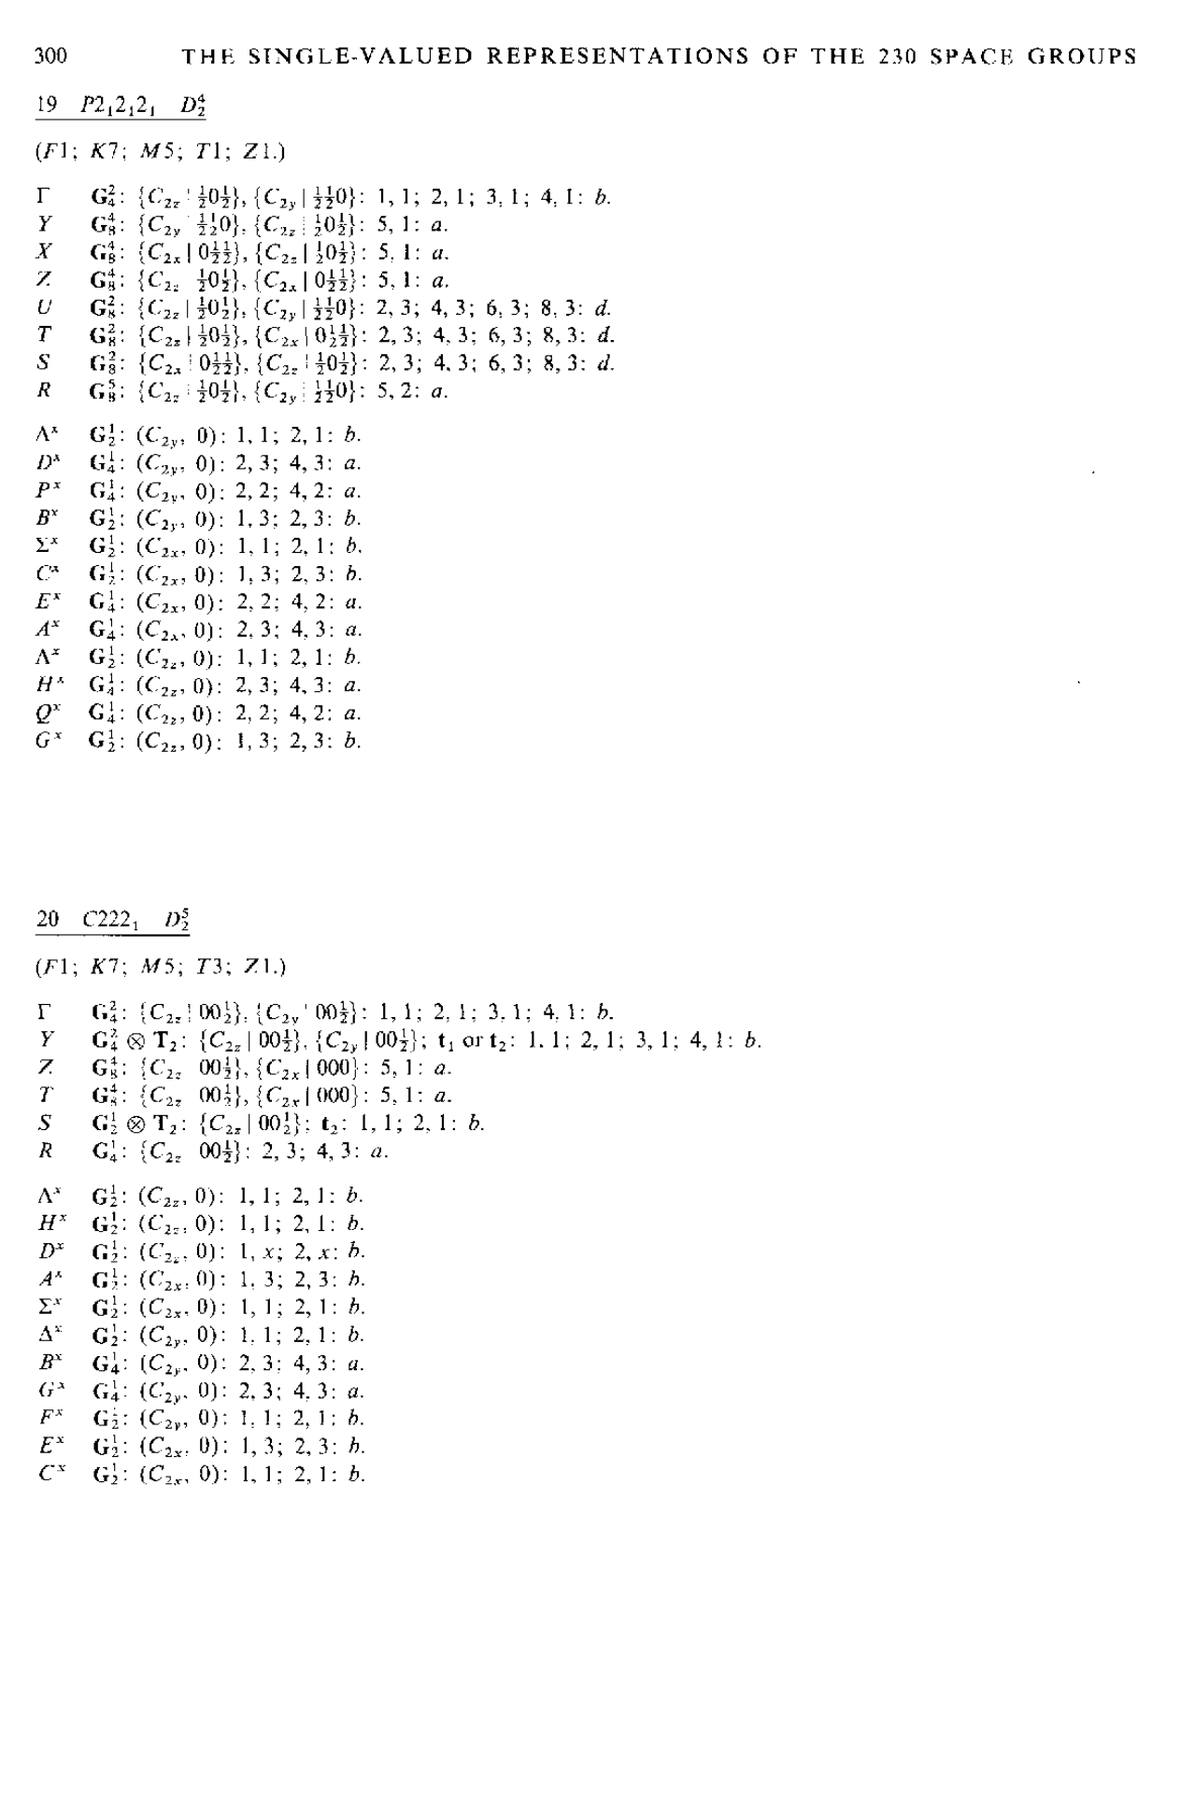
\includegraphics[width=0.86\textwidth]{c5_52_p313.jpg}
\caption*{原书第 300 页}
\end{figure}
\begin{figure}[H]
\centering
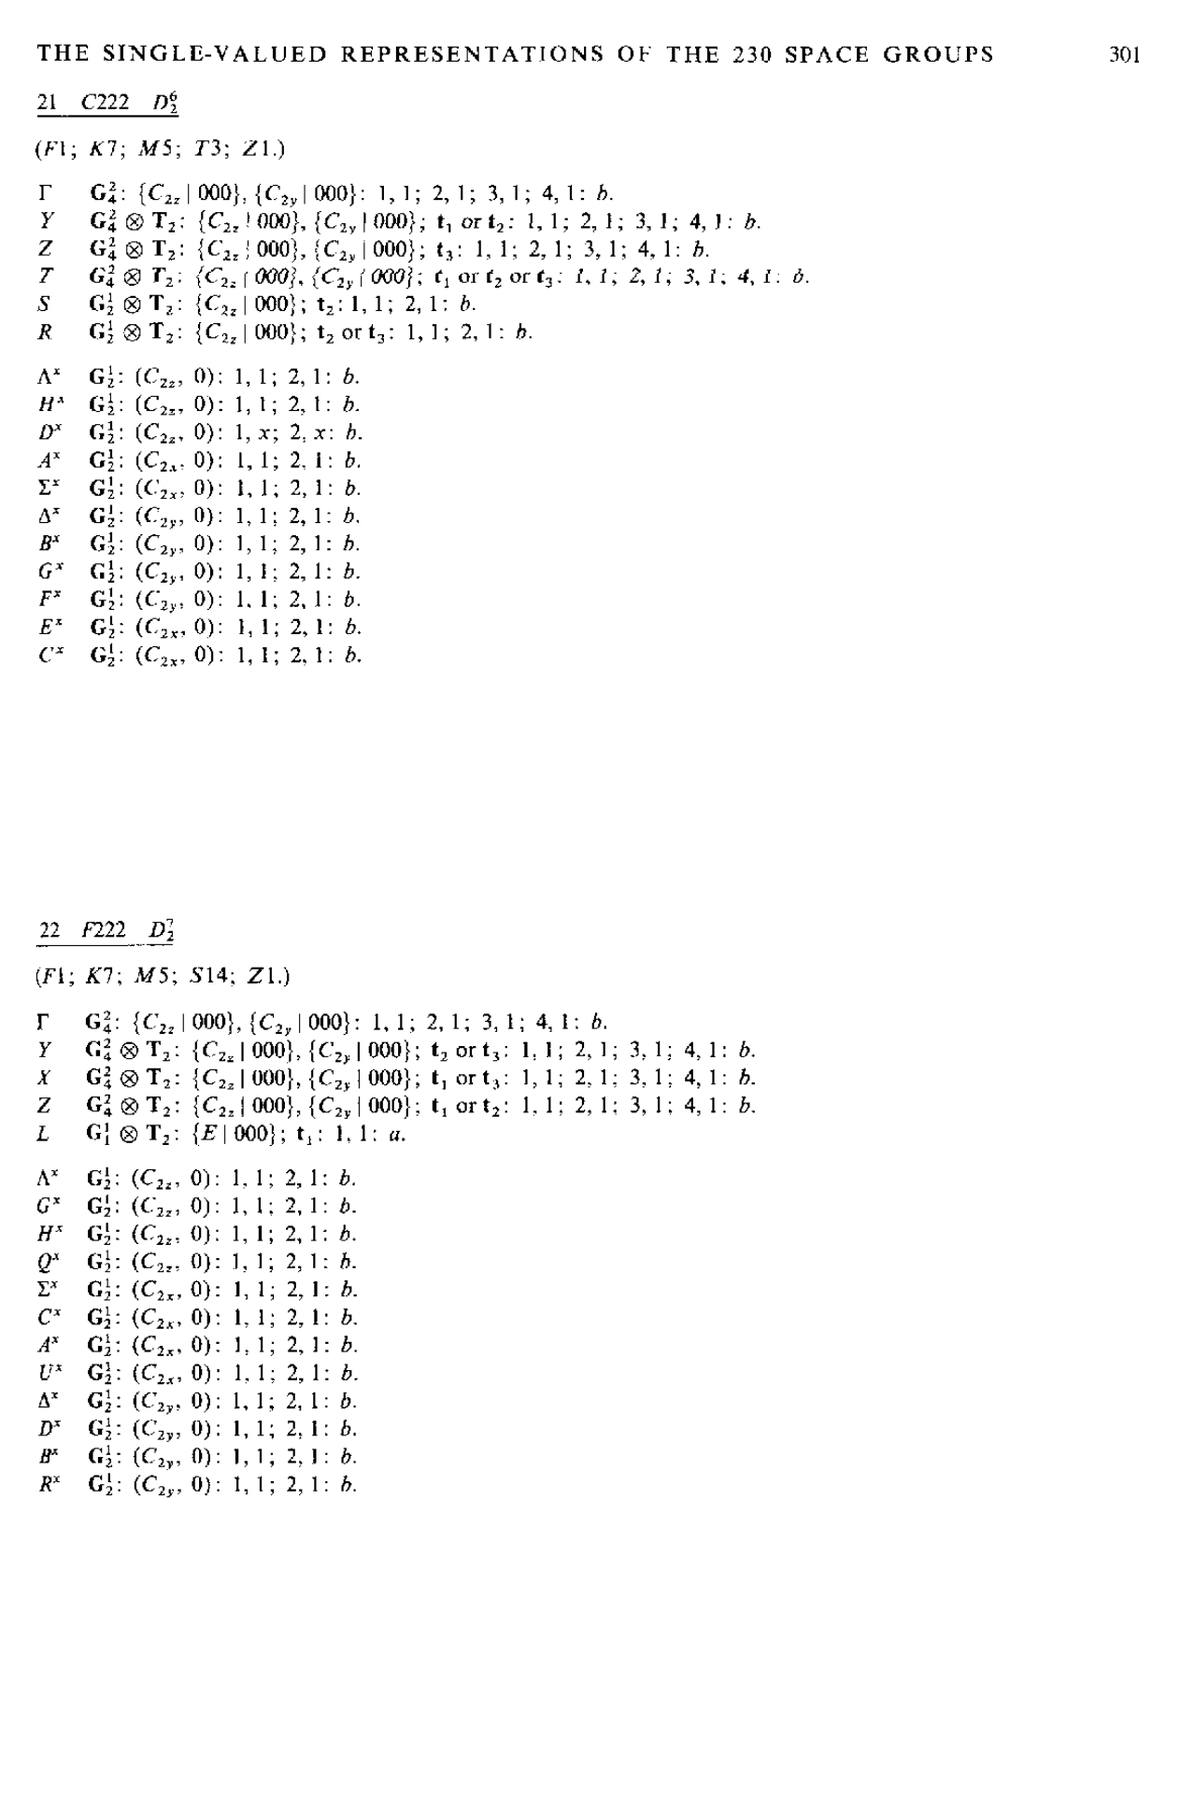
\includegraphics[width=0.86\textwidth]{c5_52_p314.jpg}
\caption*{原书第 301 页}
\end{figure}
\begin{figure}[H]
\centering
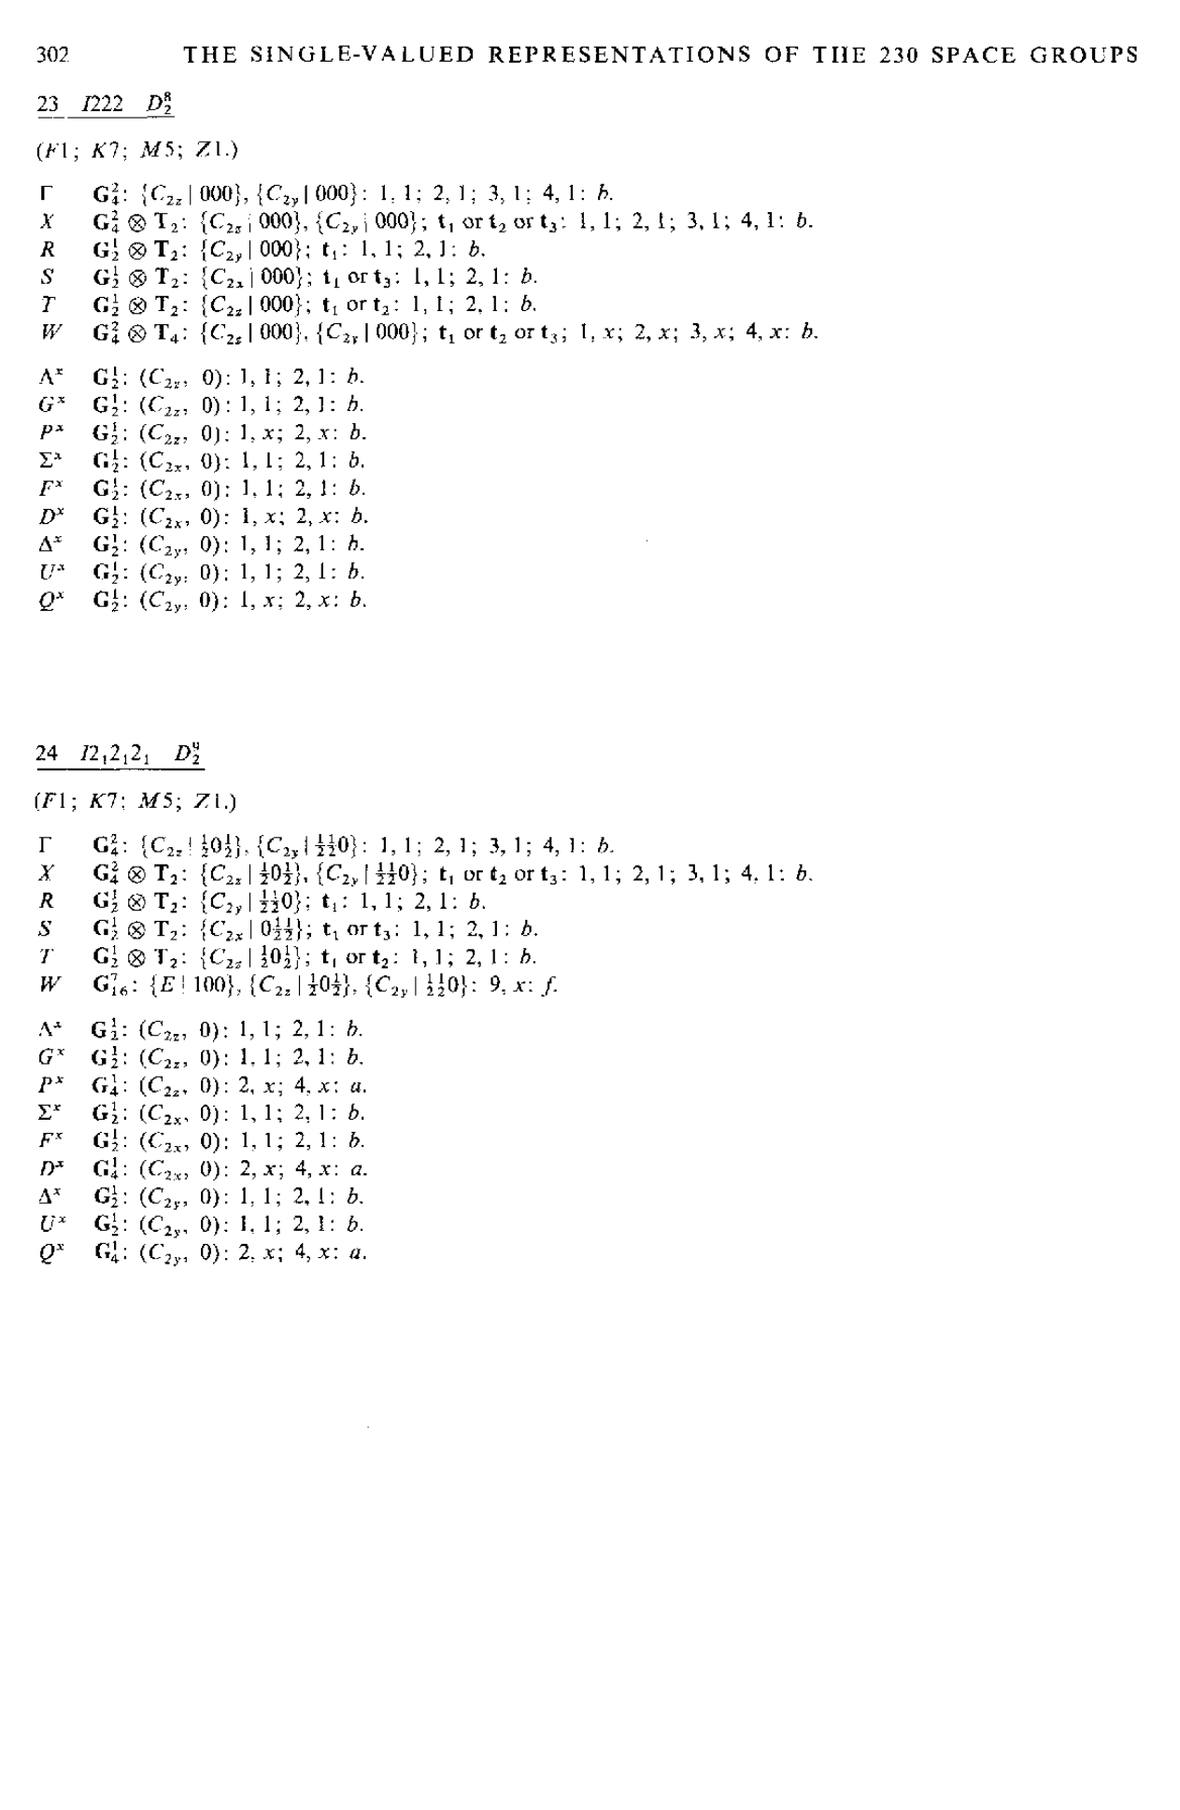
\includegraphics[width=0.86\textwidth]{c5_52_p315.jpg}
\caption*{原书第 302 页}
\end{figure}
\begin{figure}[H]
\centering
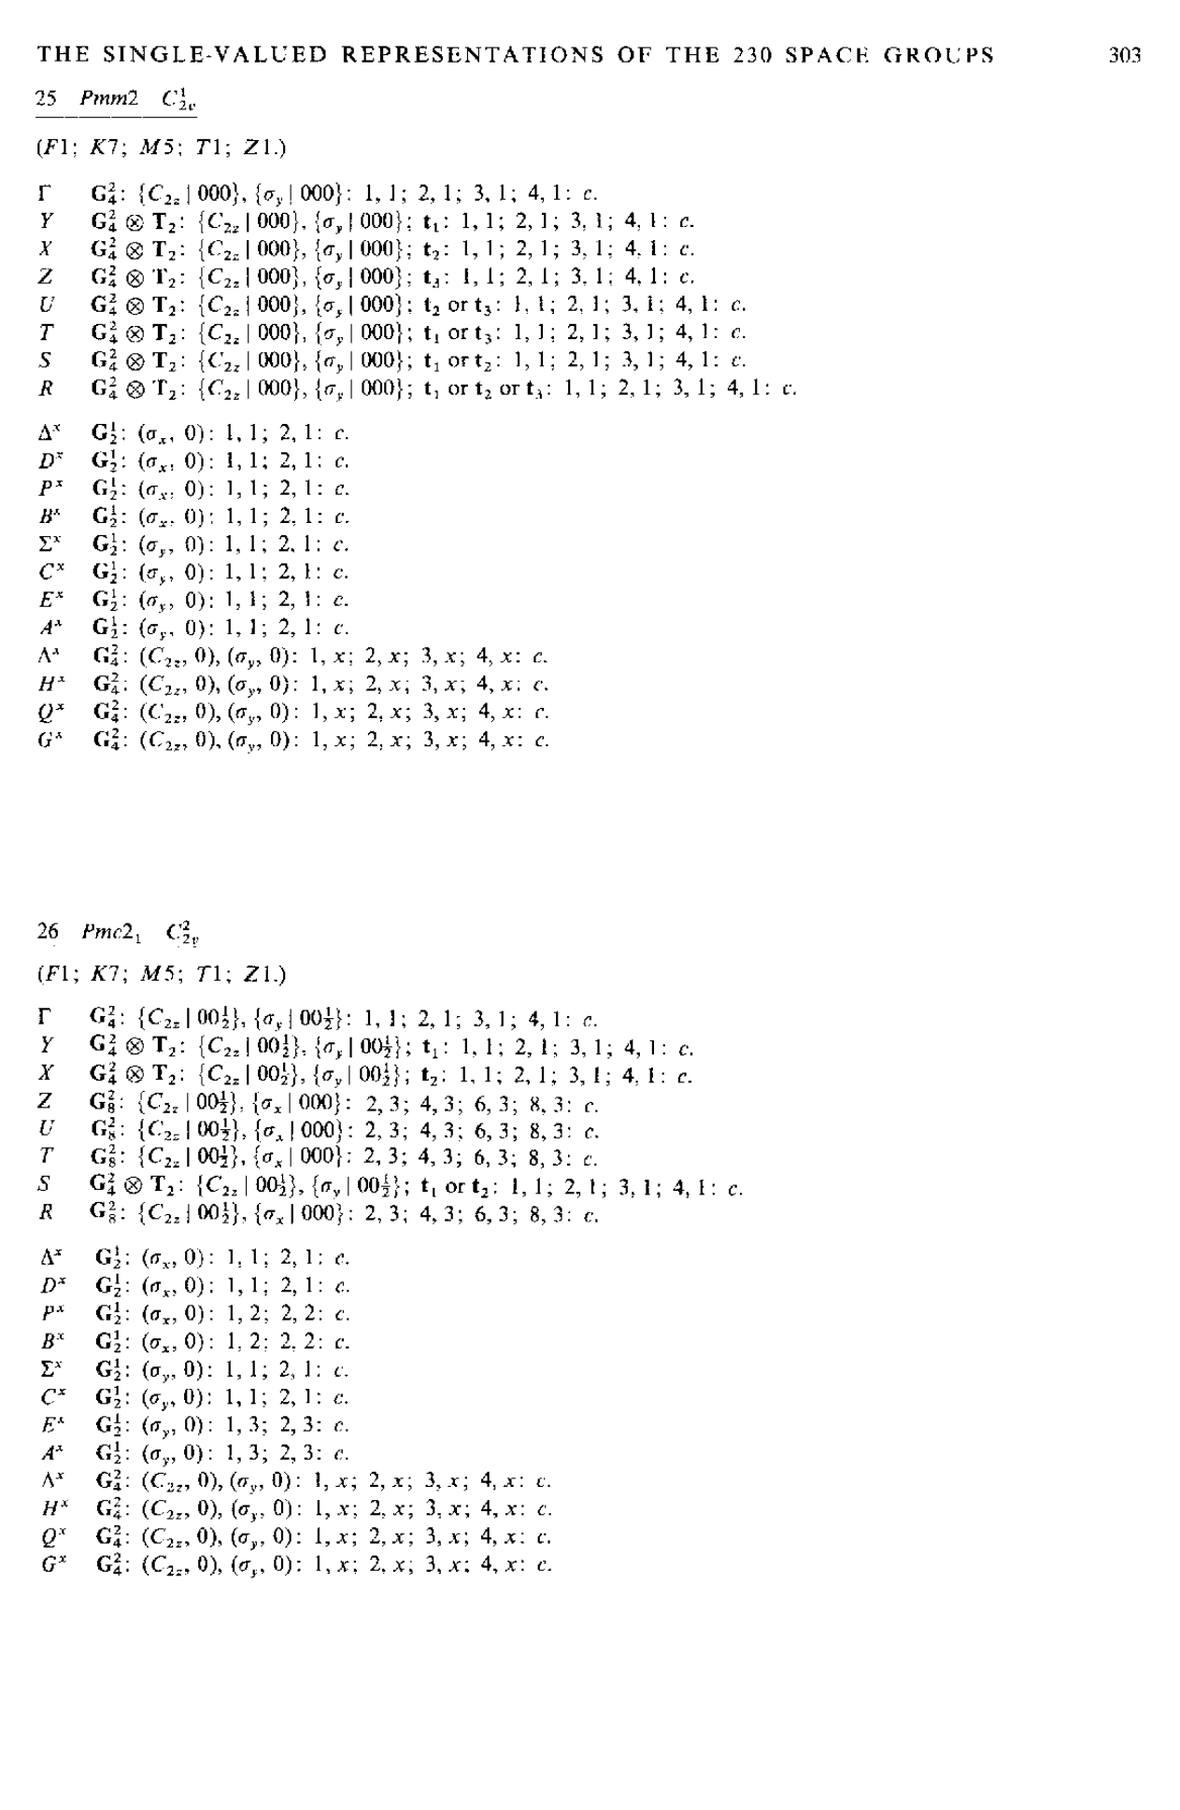
\includegraphics[width=0.86\textwidth]{c5_52_p316.jpg}
\caption*{原书第 303 页}
\end{figure}
\begin{figure}[H]
\centering
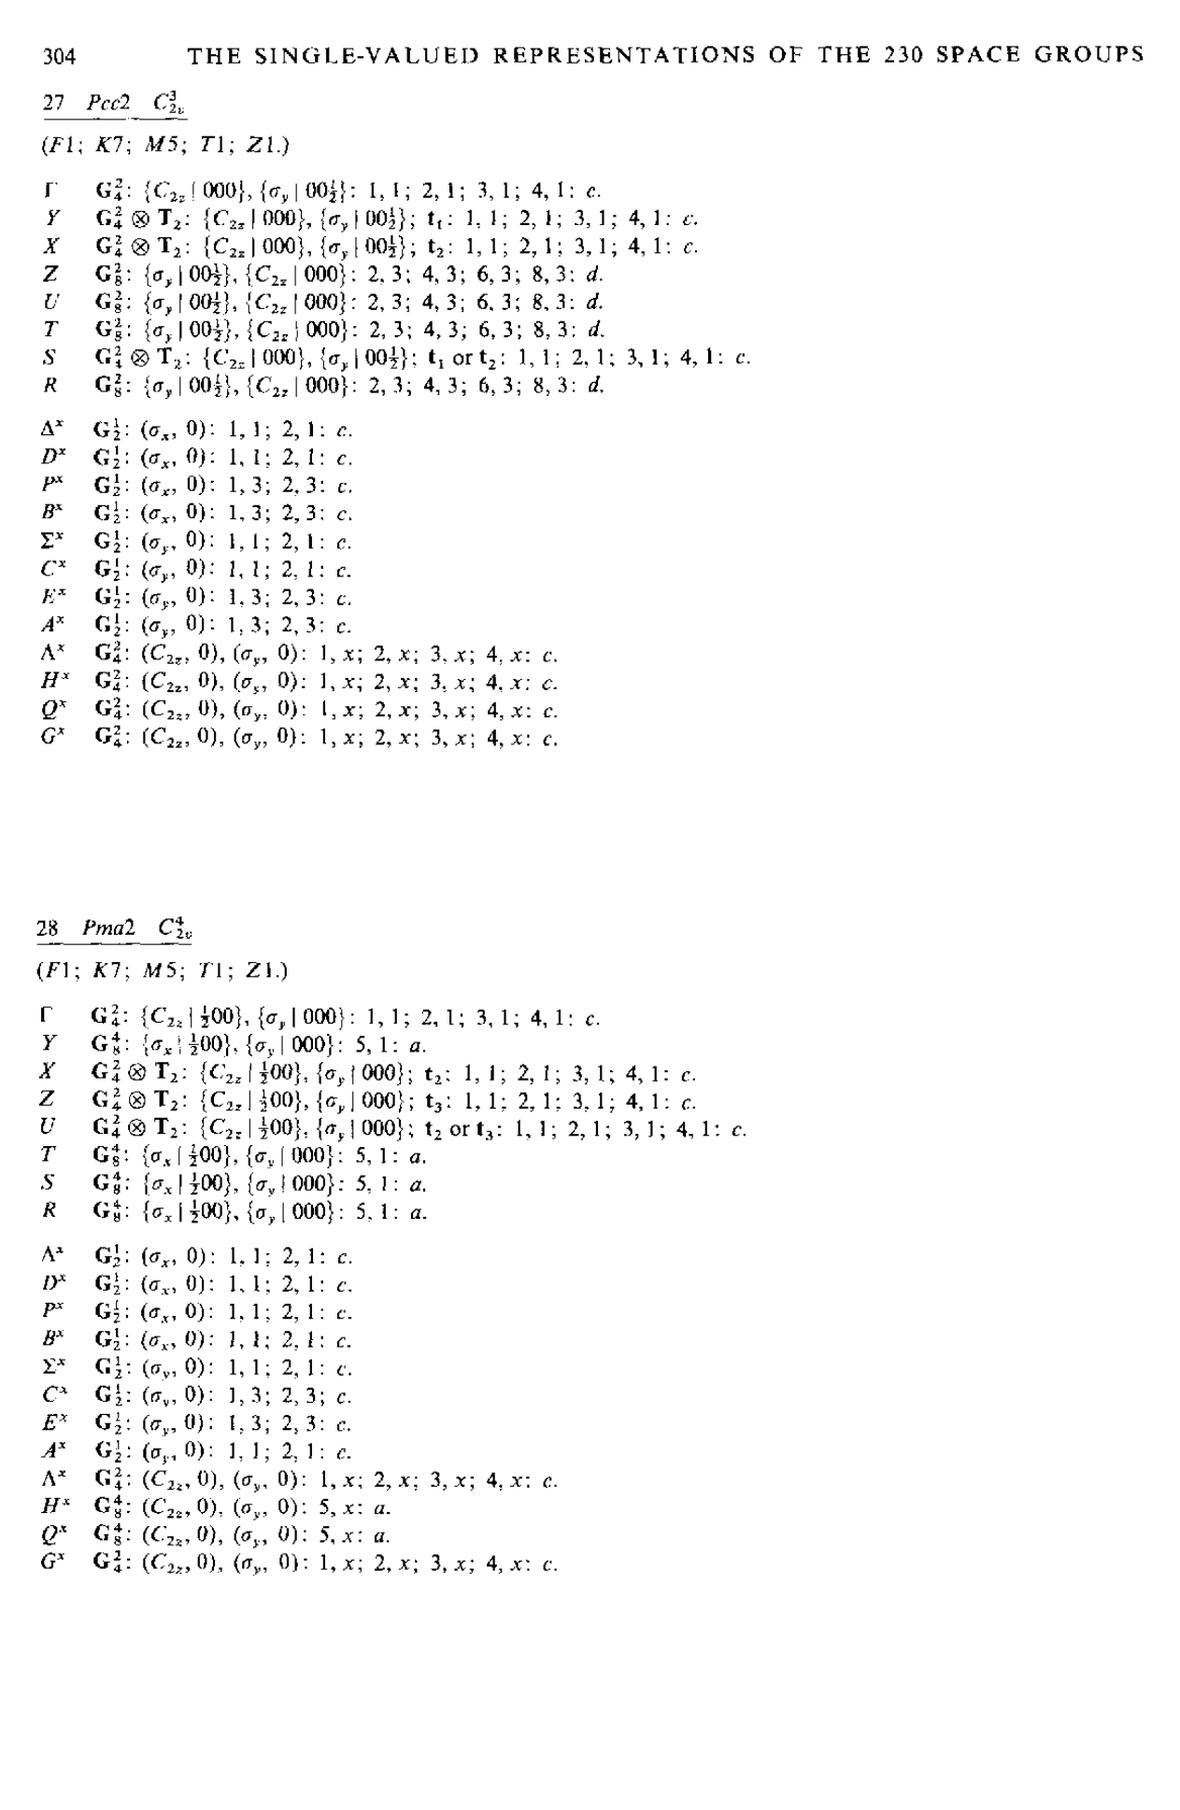
\includegraphics[width=0.86\textwidth]{c5_52_p317.jpg}
\caption*{原书第 304 页}
\end{figure}
\begin{figure}[H]
\centering
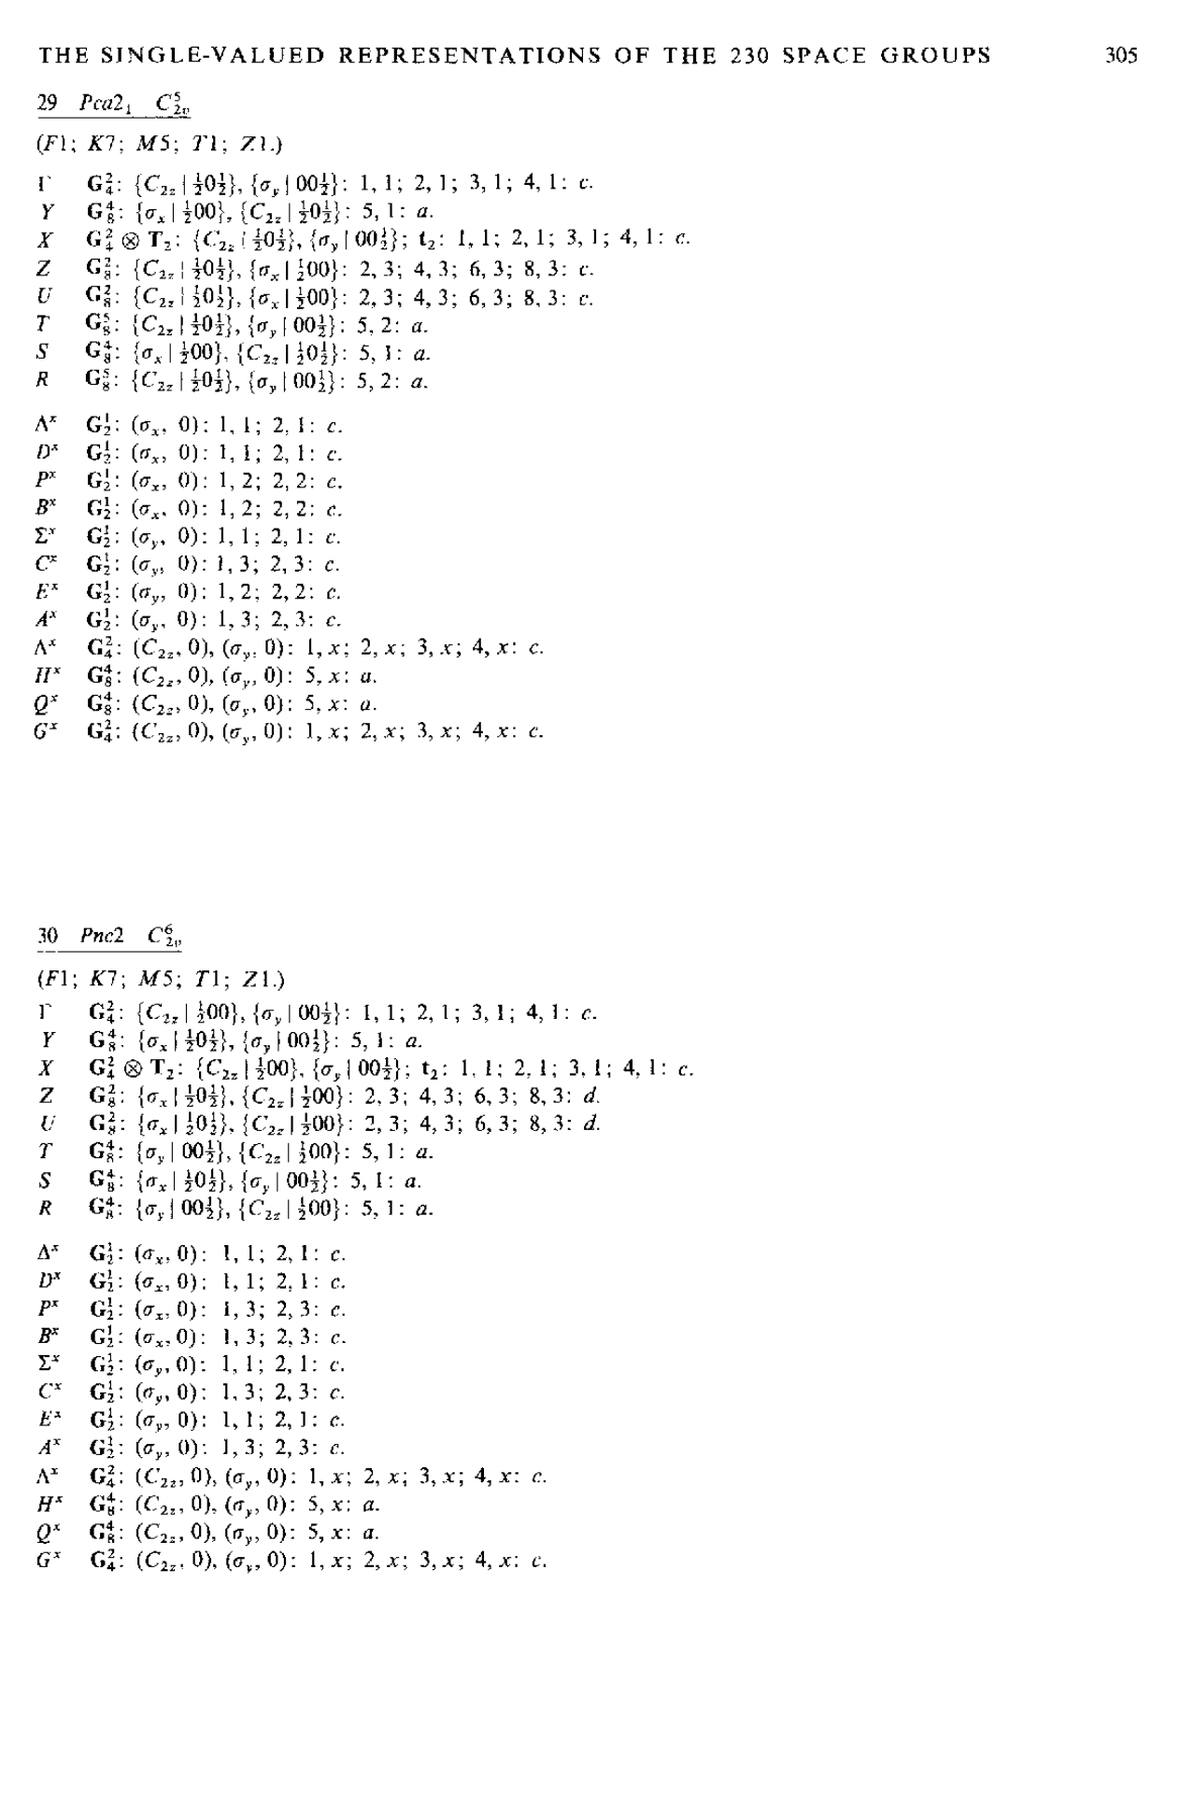
\includegraphics[width=0.86\textwidth]{c5_52_p318.jpg}
\caption*{原书第 305 页}
\end{figure}
\begin{figure}[H]
\centering
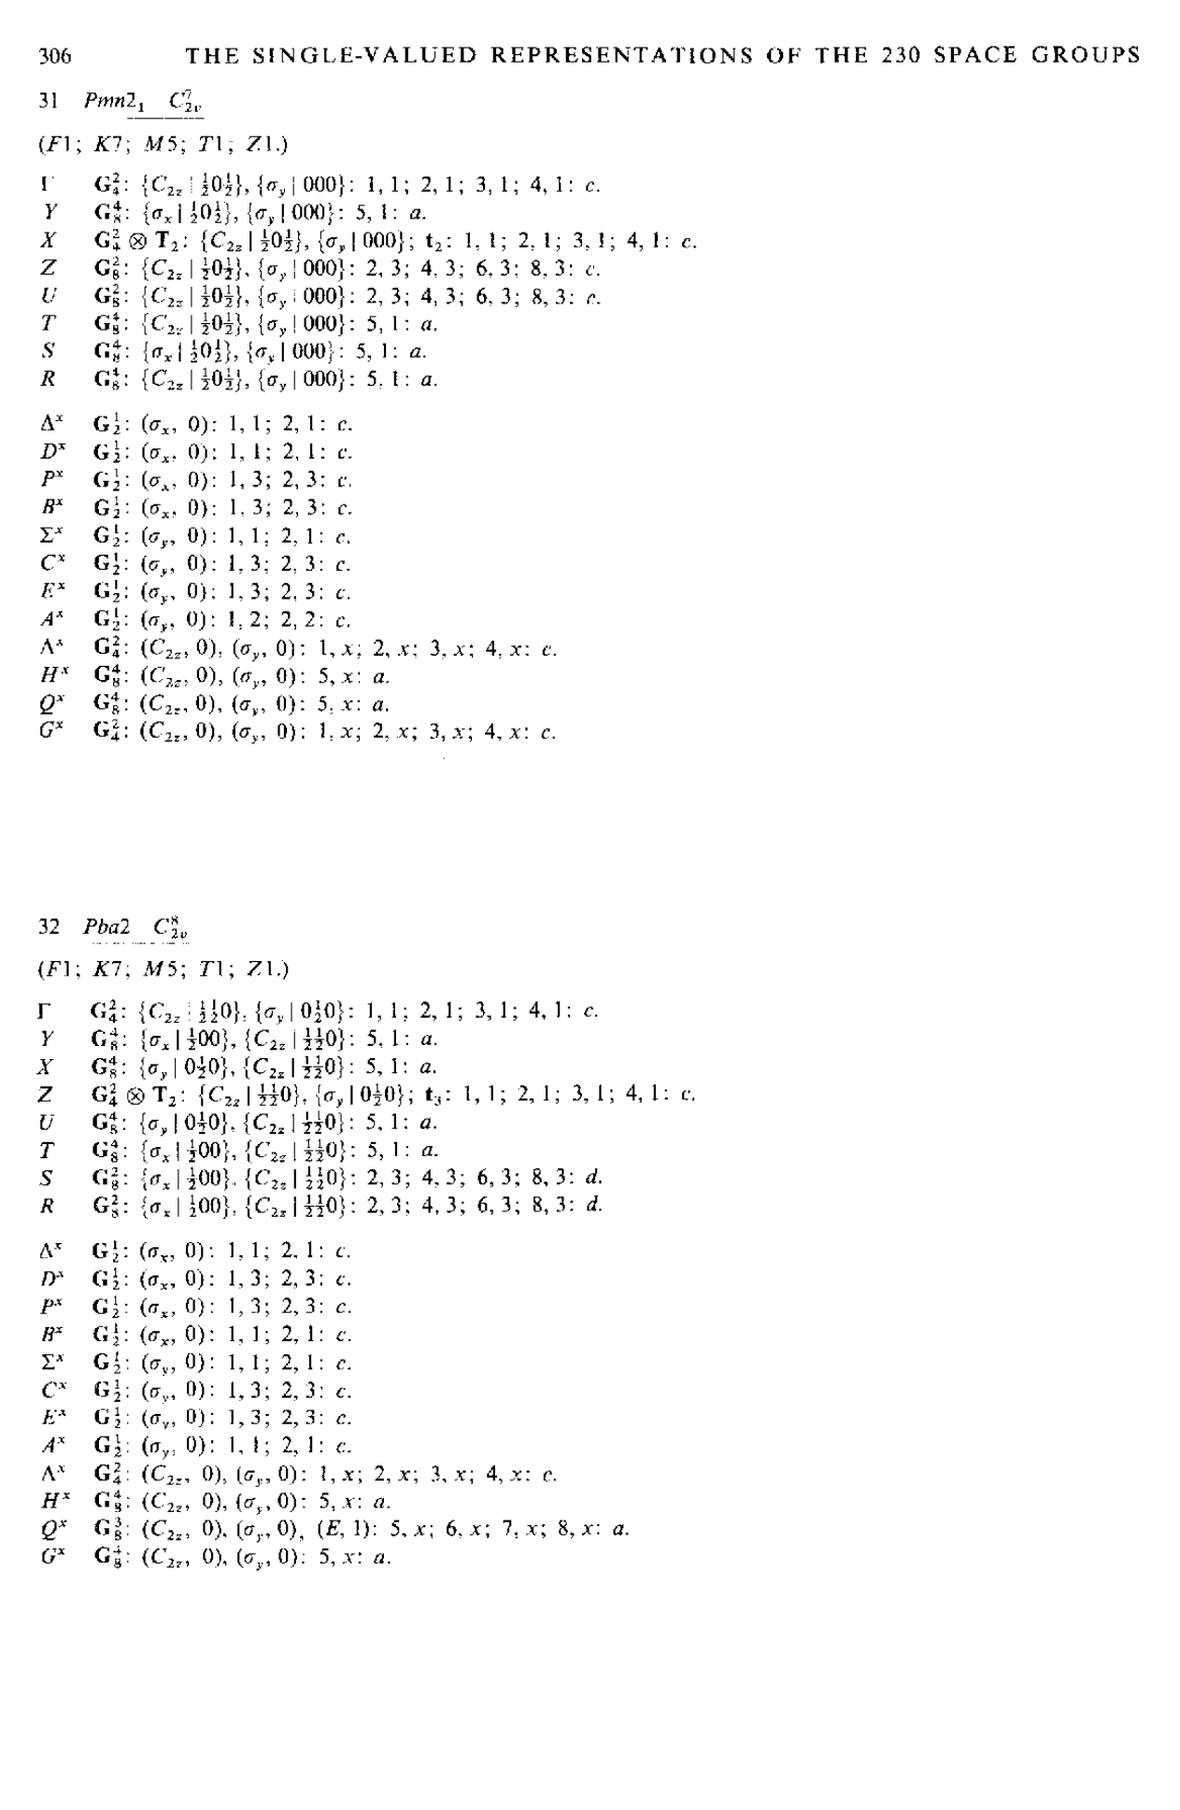
\includegraphics[width=0.86\textwidth]{c5_52_p319.jpg}
\caption*{原书第 306 页}
\end{figure}
\begin{figure}[H]
\centering
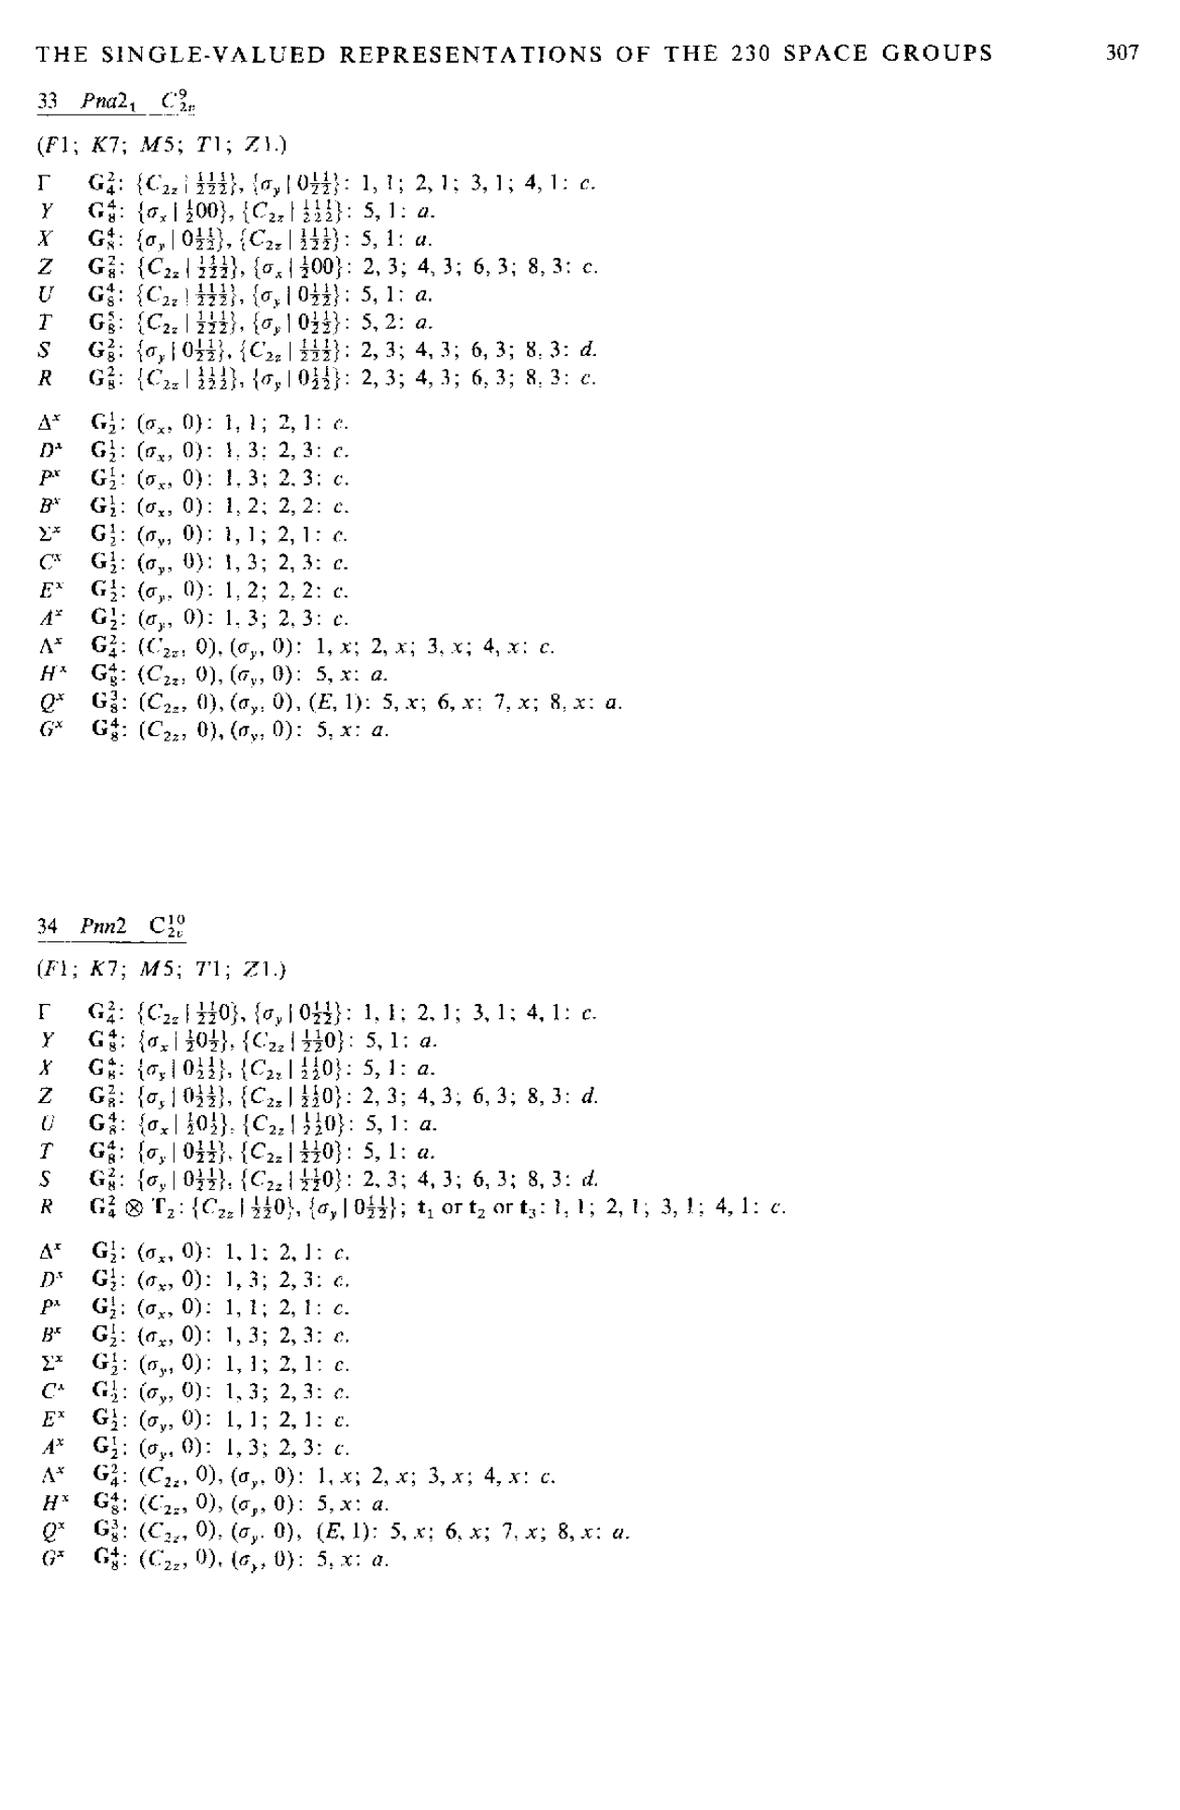
\includegraphics[width=0.86\textwidth]{c5_52_p320.jpg}
\caption*{原书第 307 页}
\end{figure}
\begin{figure}[H]
\centering
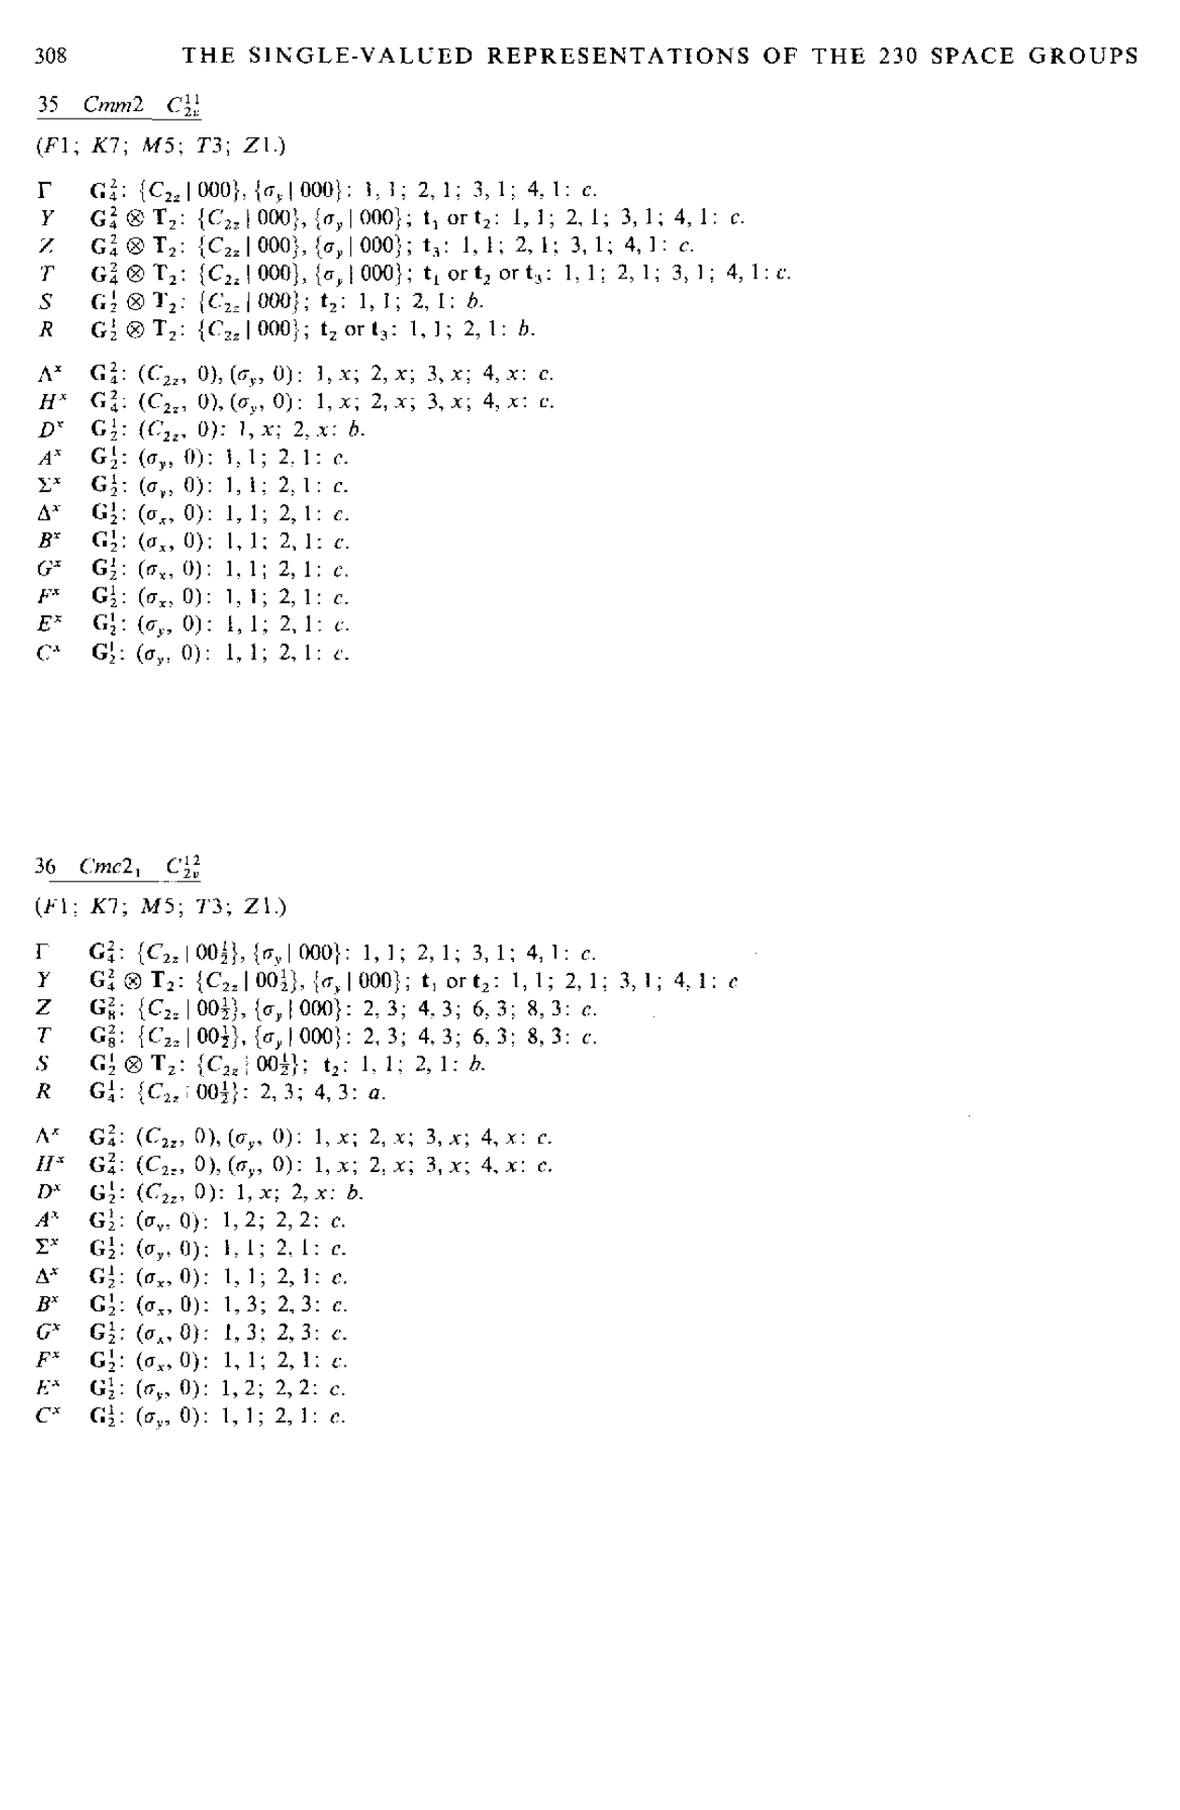
\includegraphics[width=0.86\textwidth]{c5_52_p321.jpg}
\caption*{原书第 308 页}
\end{figure}
\begin{figure}[H]
\centering
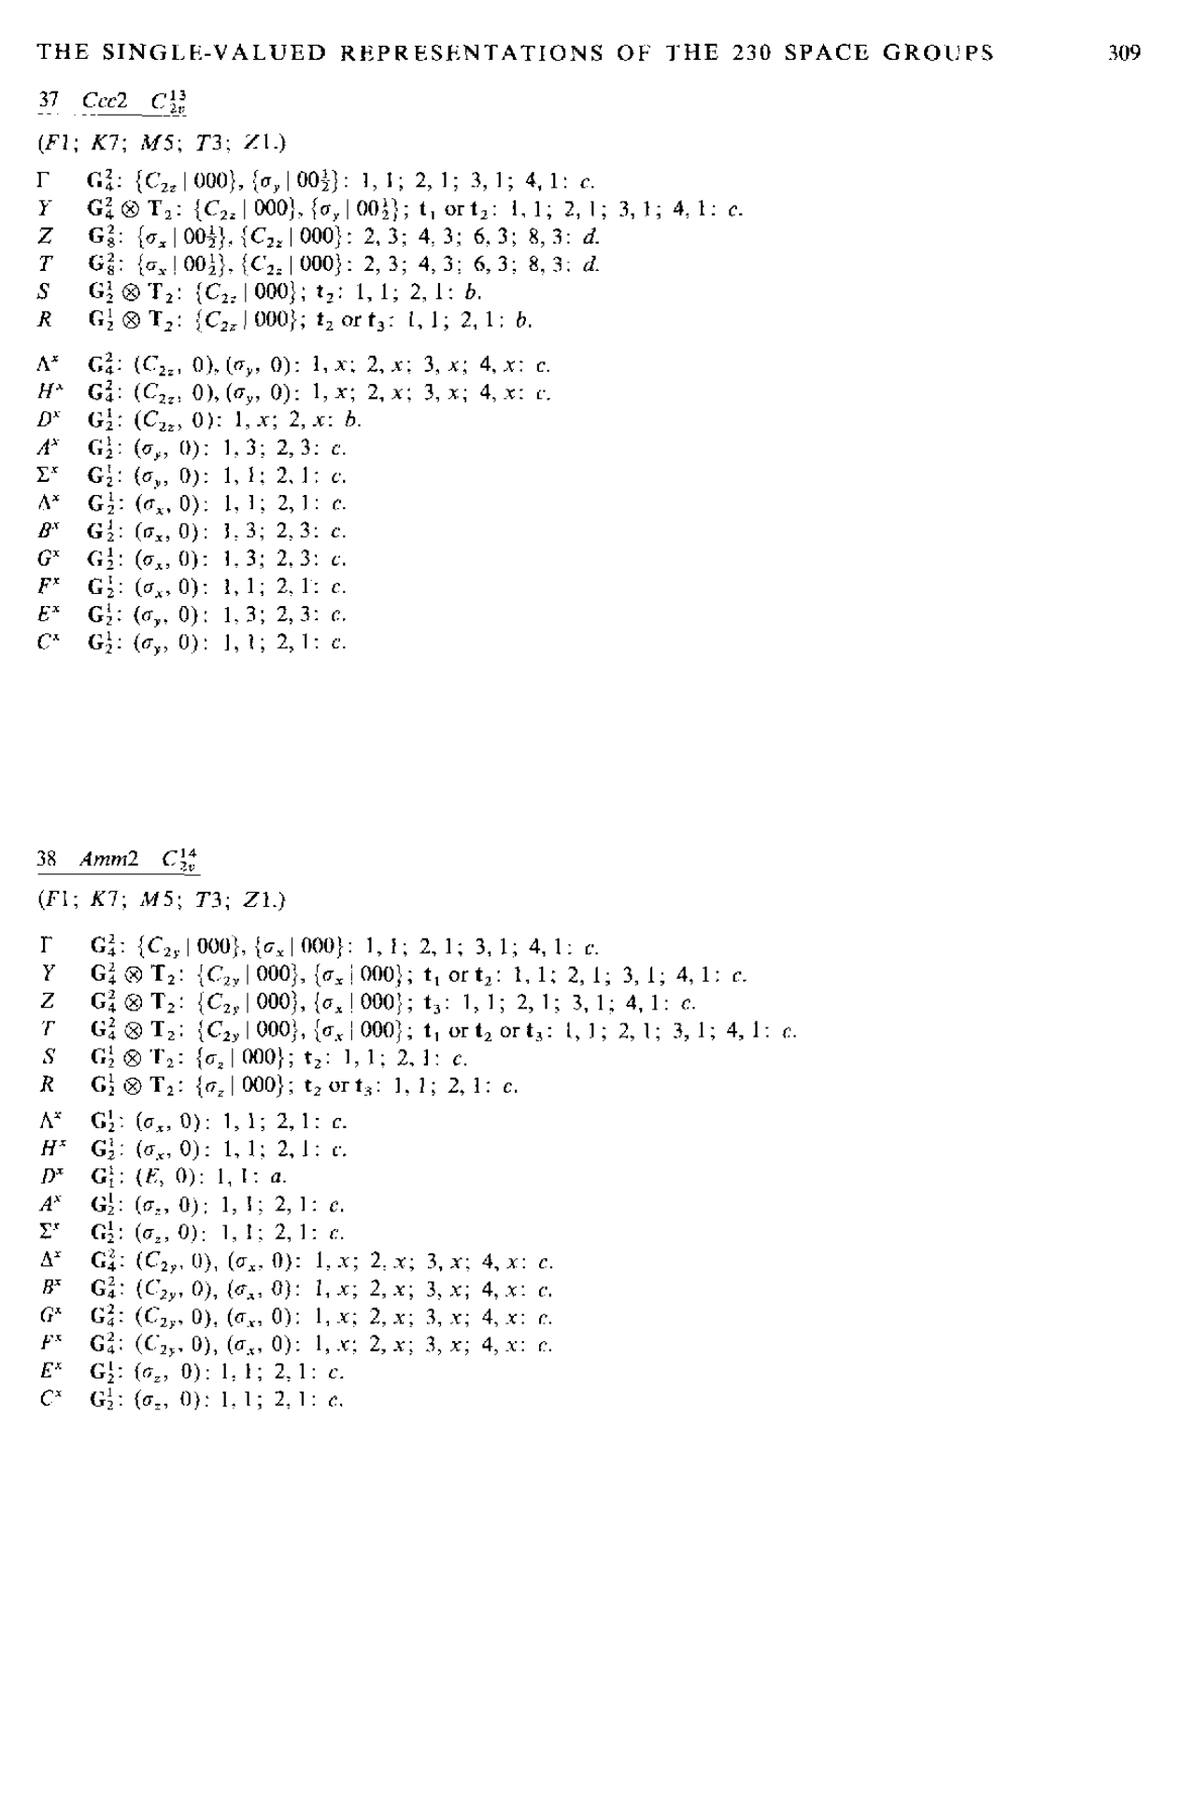
\includegraphics[width=0.86\textwidth]{c5_52_p322.jpg}
\caption*{原书第 309 页}
\end{figure}
\begin{figure}[H]
\centering
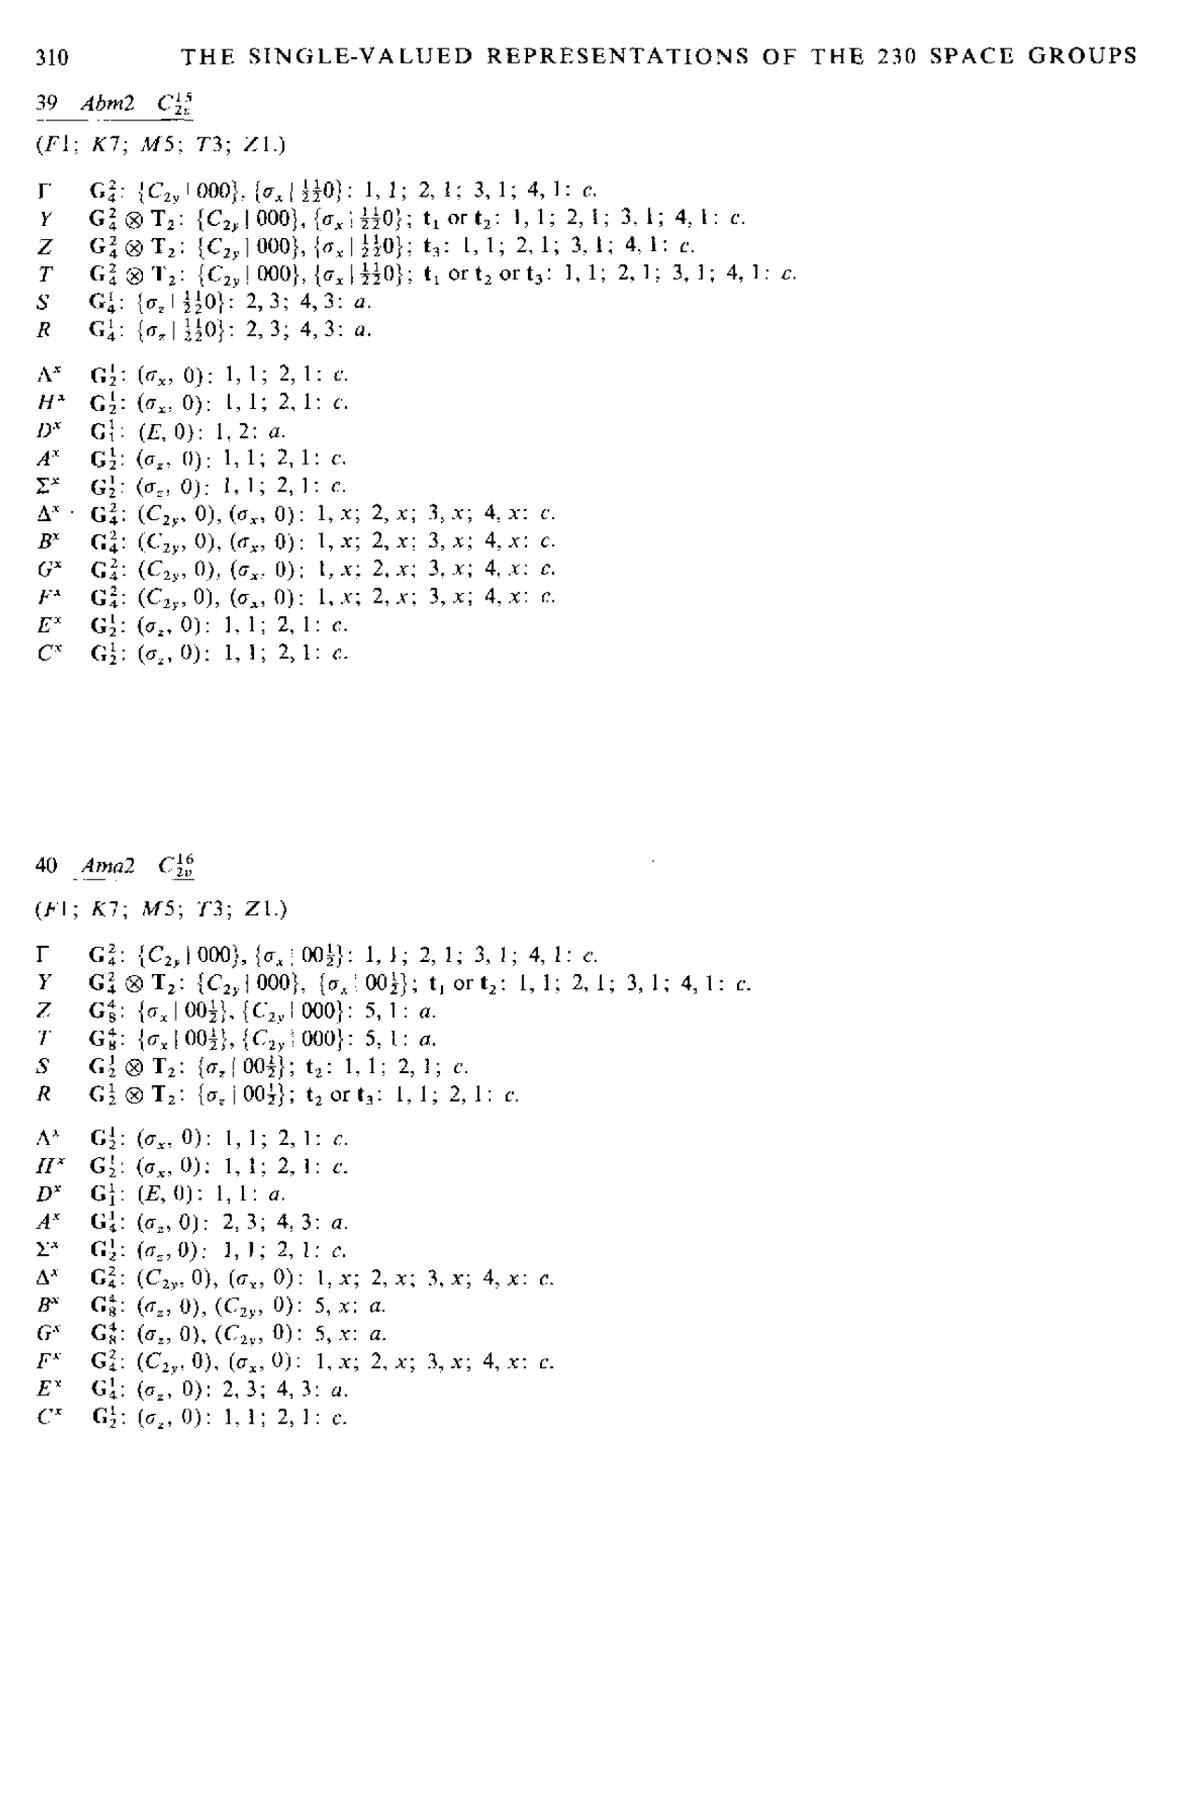
\includegraphics[width=0.86\textwidth]{c5_52_p323.jpg}
\caption*{原书第 310 页}
\end{figure}
\begin{figure}[H]
\centering
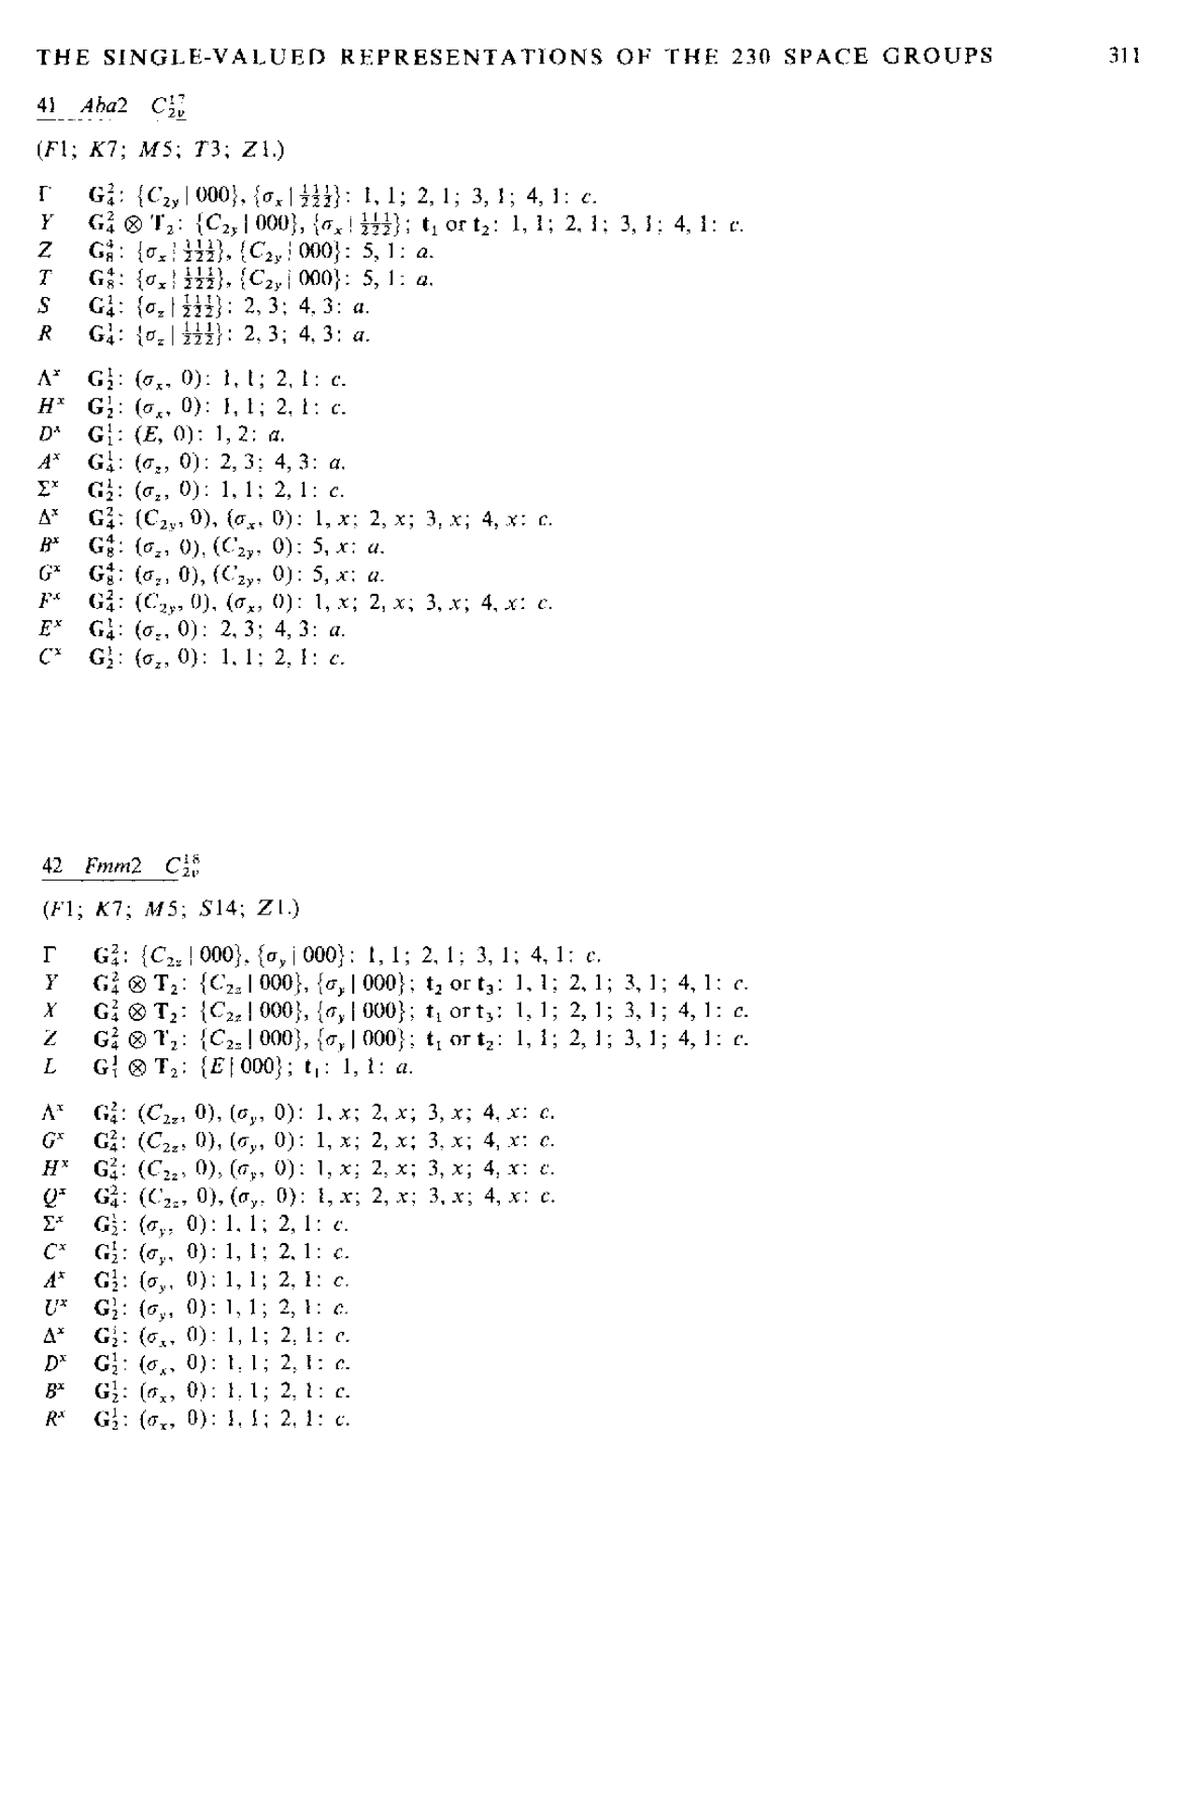
\includegraphics[width=0.86\textwidth]{c5_52_p324.jpg}
\caption*{原书第 311 页}
\end{figure}
\begin{figure}[H]
\centering
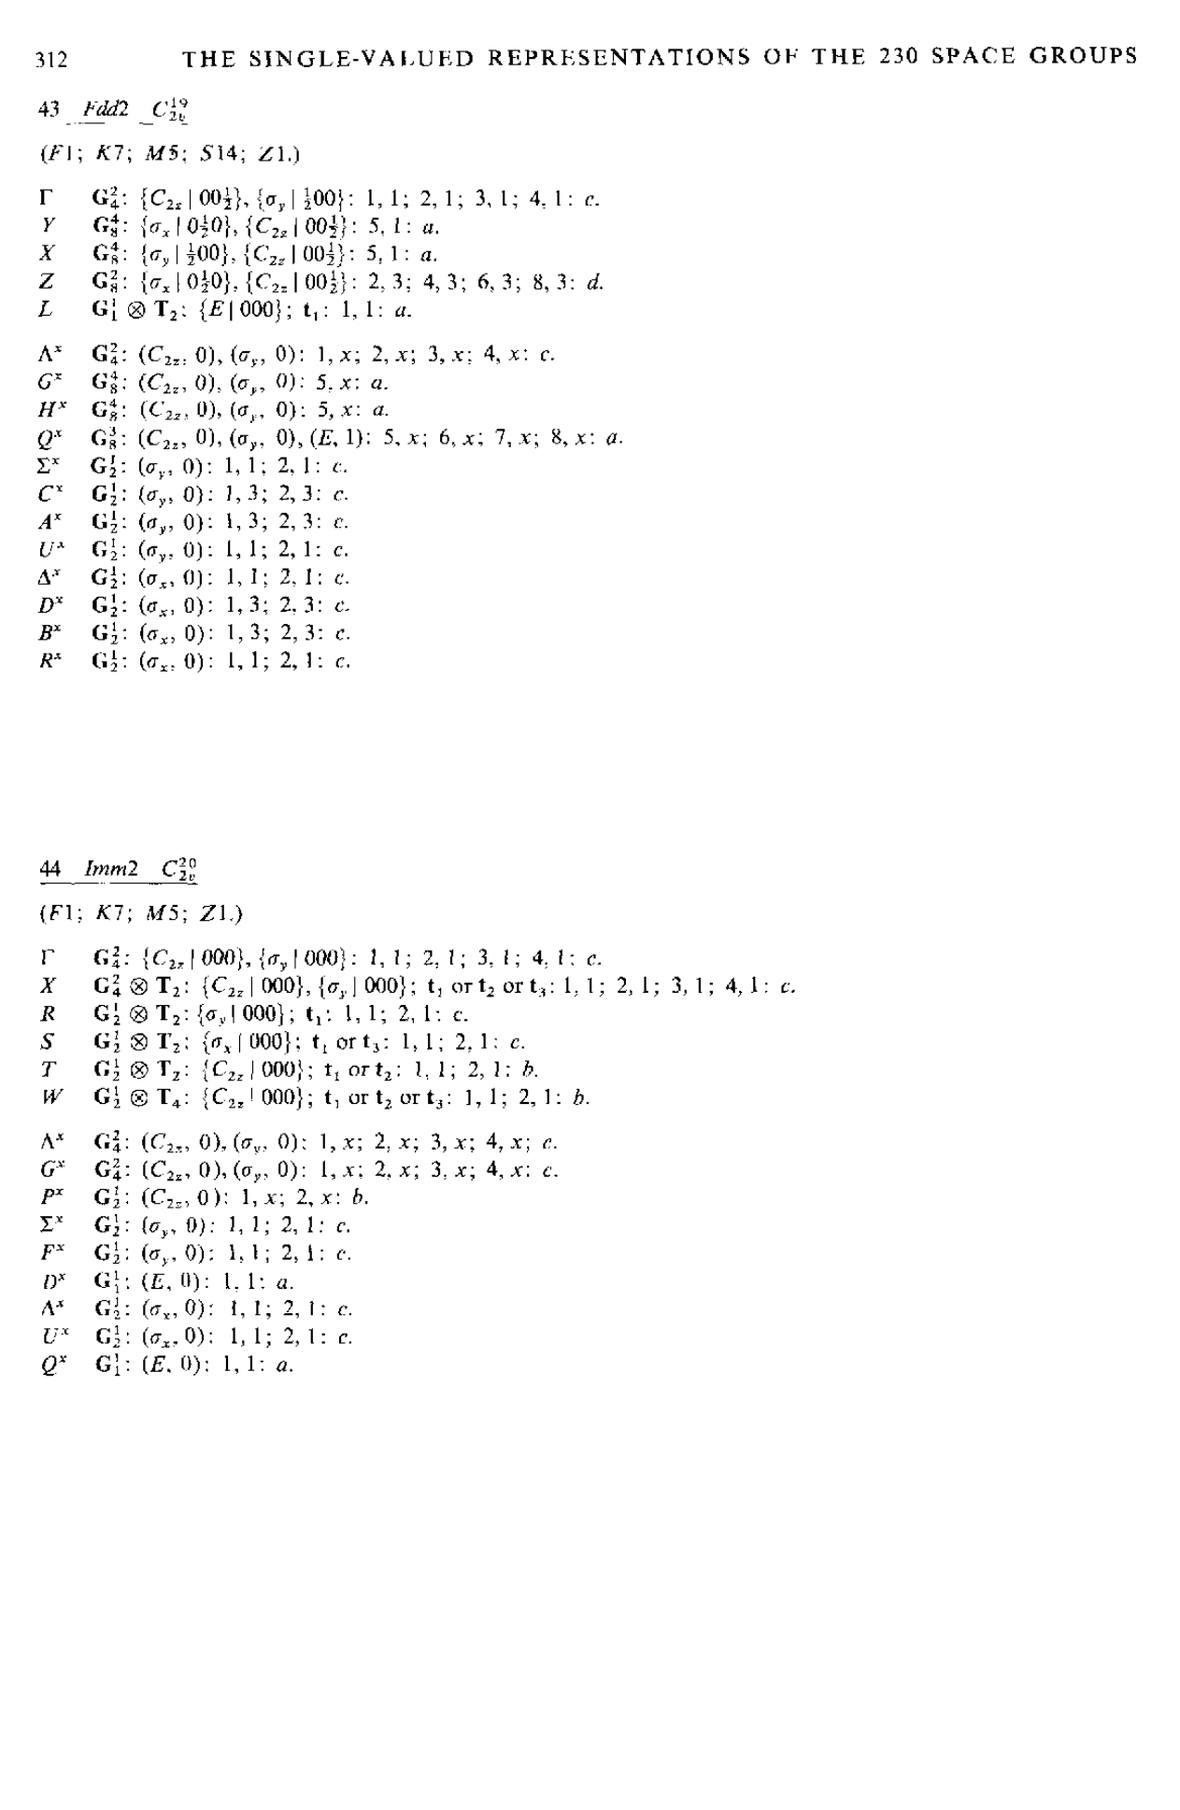
\includegraphics[width=0.86\textwidth]{c5_52_p325.jpg}
\caption*{原书第 312 页}
\end{figure}
\begin{figure}[H]
\centering
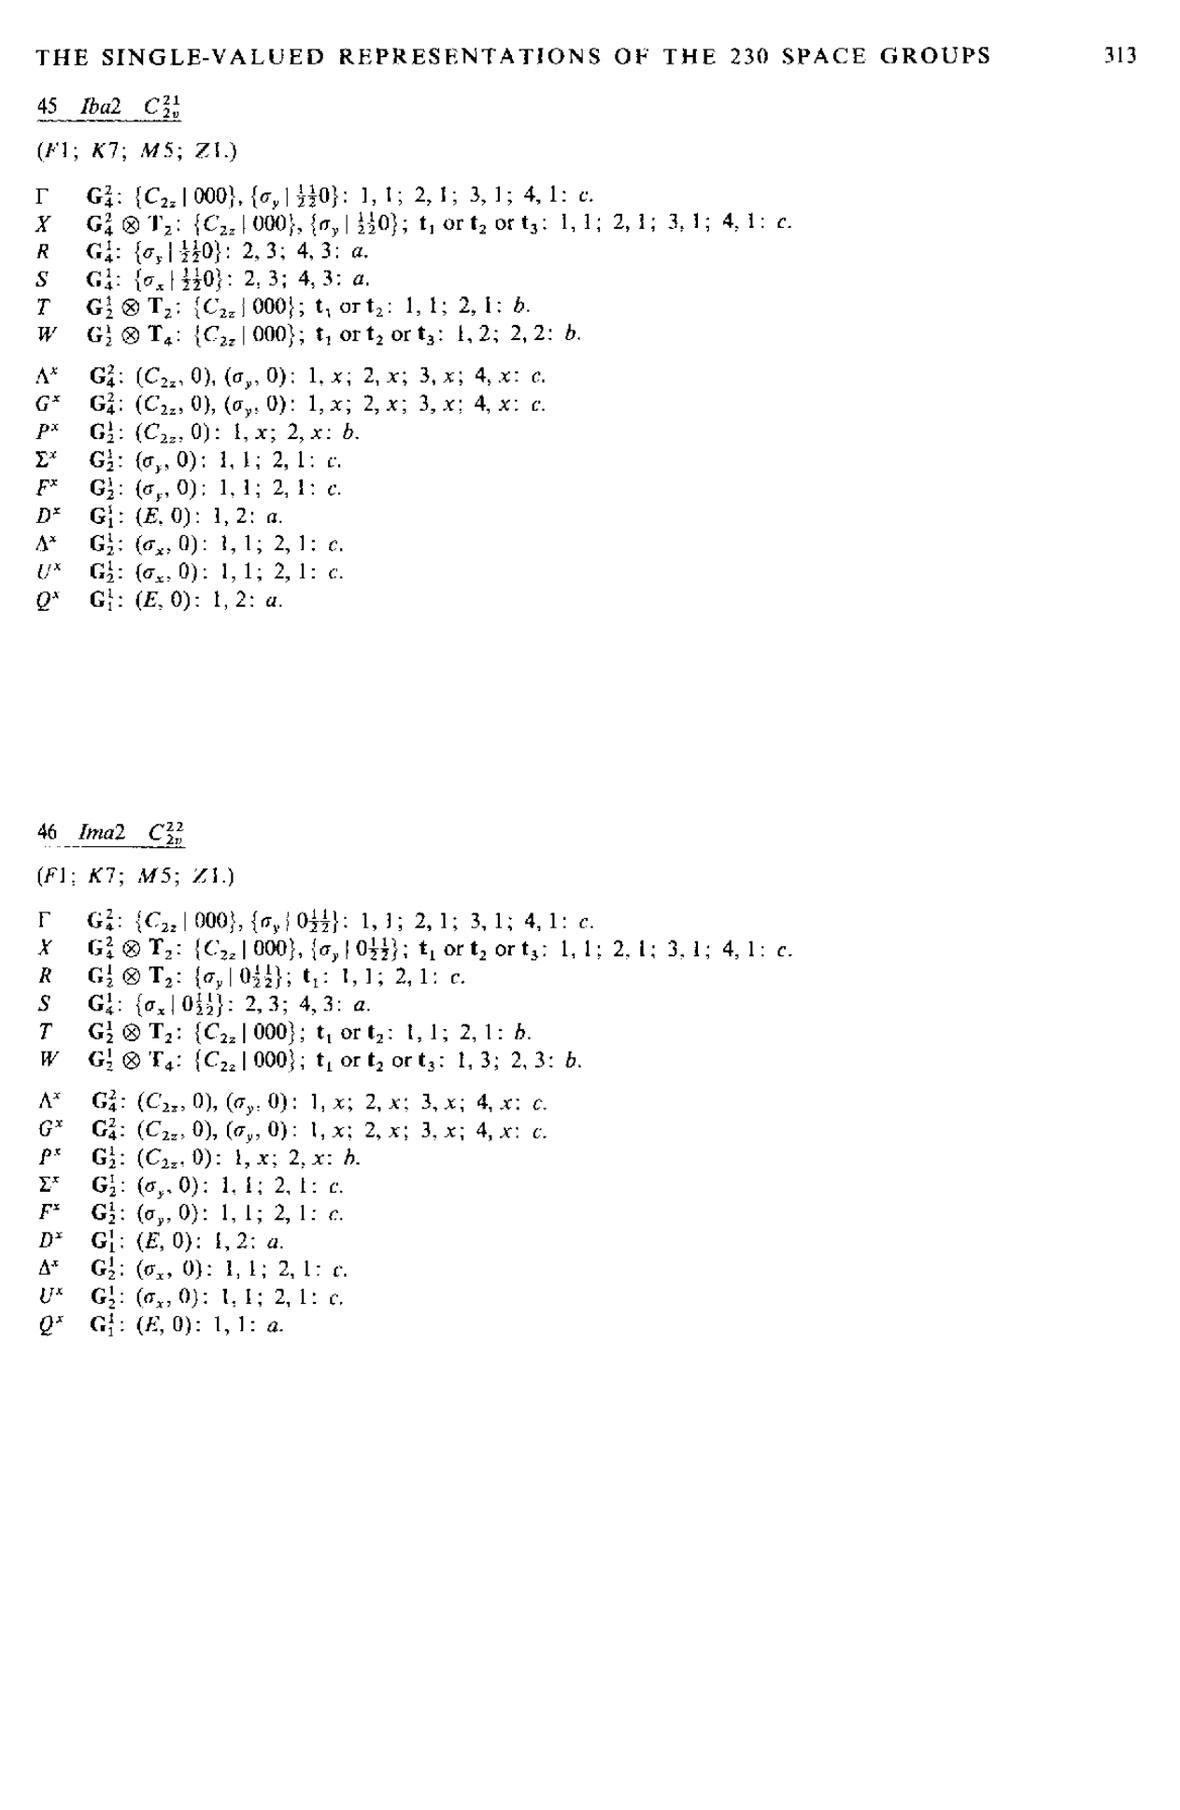
\includegraphics[width=0.86\textwidth]{c5_52_p326.jpg}
\caption*{原书第 313 页}
\end{figure}
\begin{figure}[H]
\centering
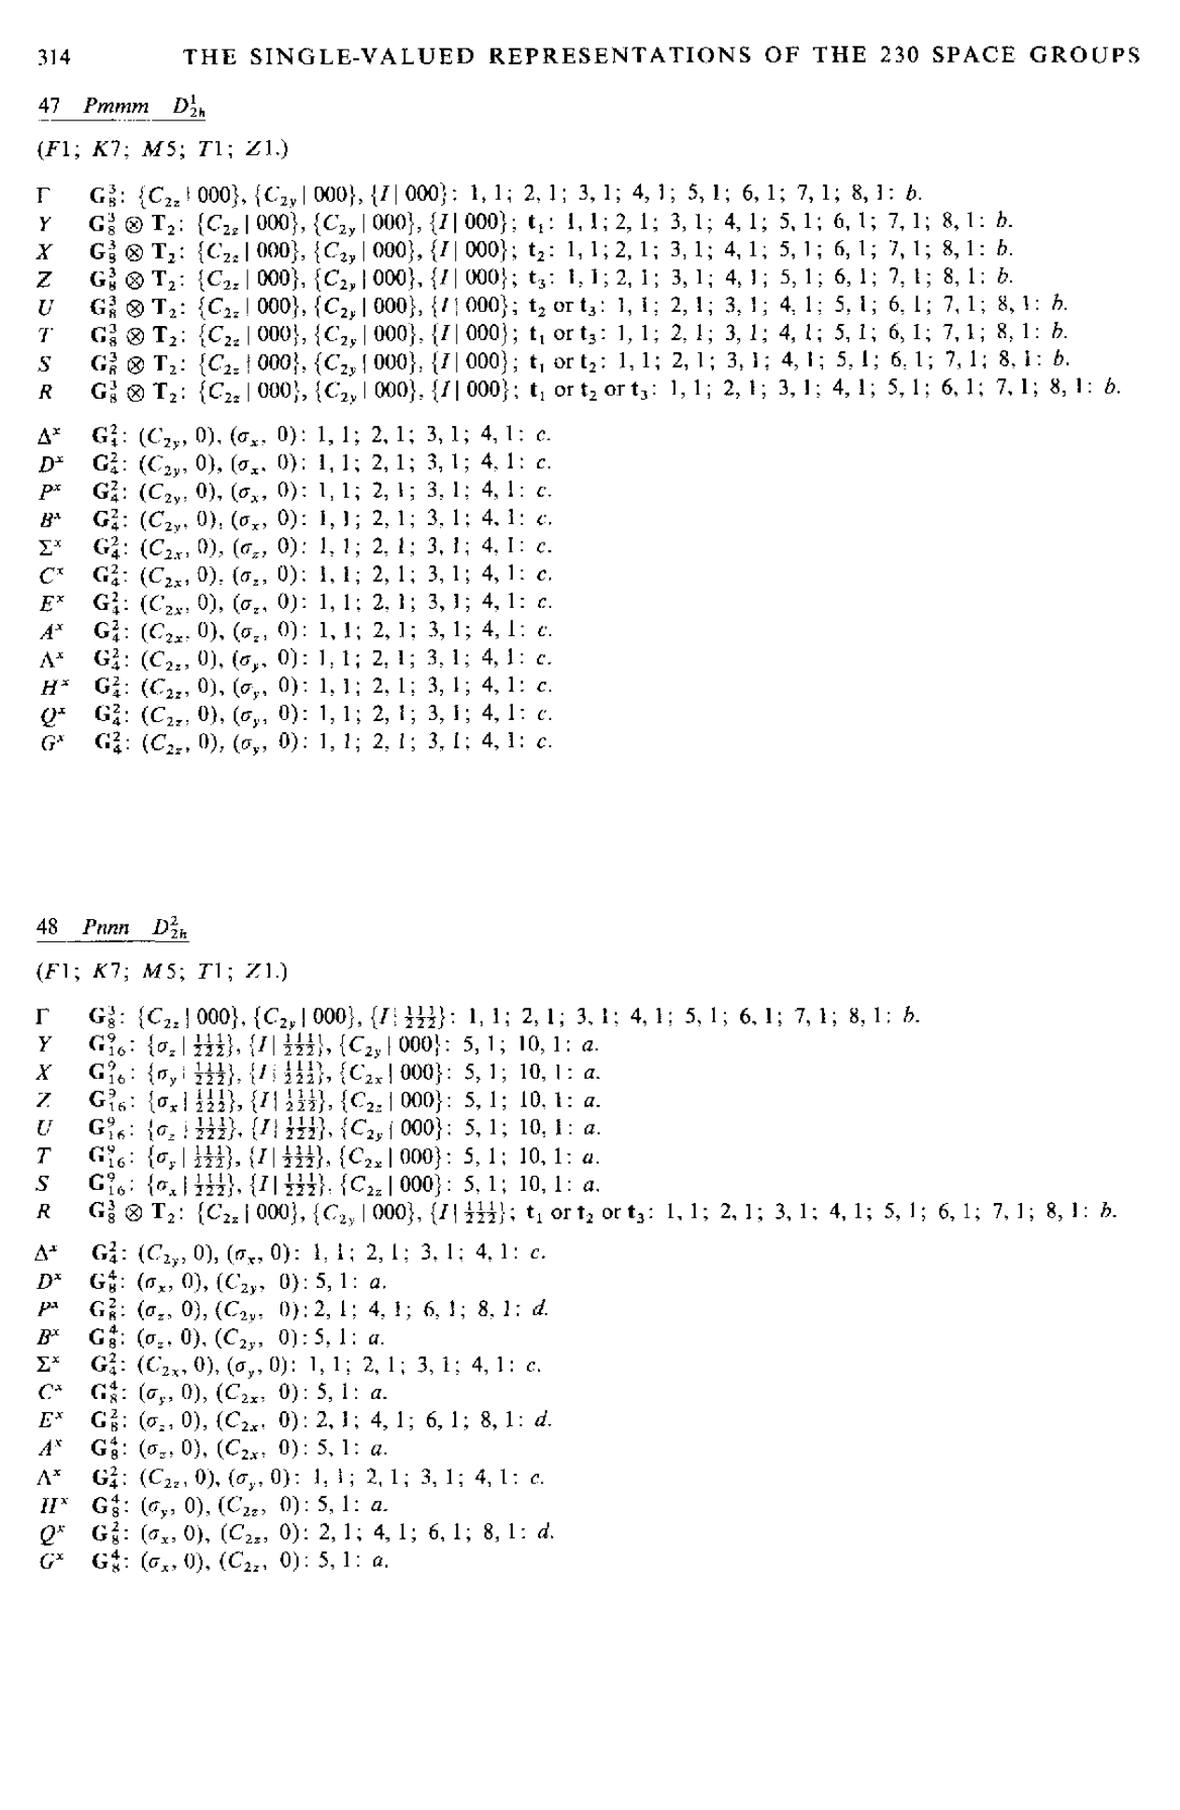
\includegraphics[width=0.86\textwidth]{c5_52_p327.jpg}
\caption*{原书第 314 页}
\end{figure}
\begin{figure}[H]
\centering
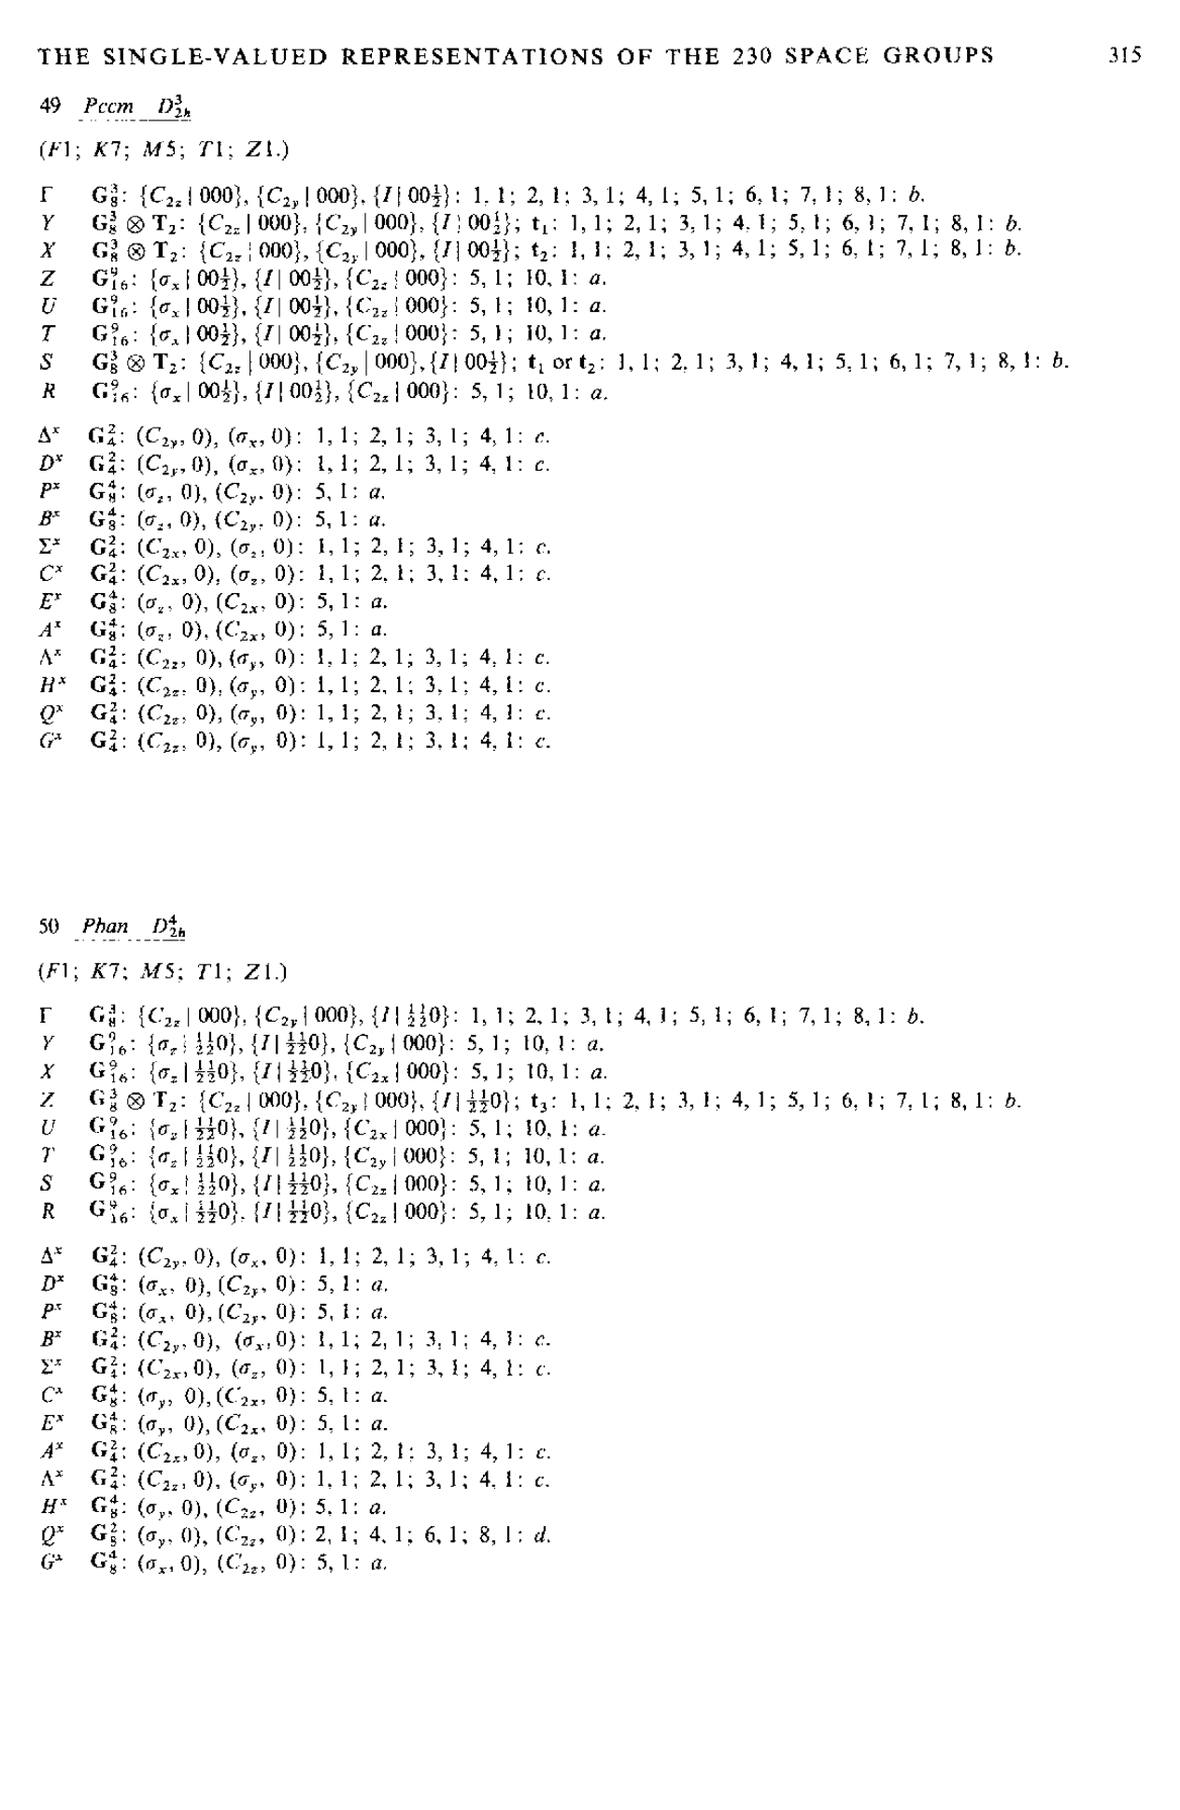
\includegraphics[width=0.86\textwidth]{c5_52_p328.jpg}
\caption*{原书第 315 页}
\end{figure}
\begin{figure}[H]
\centering
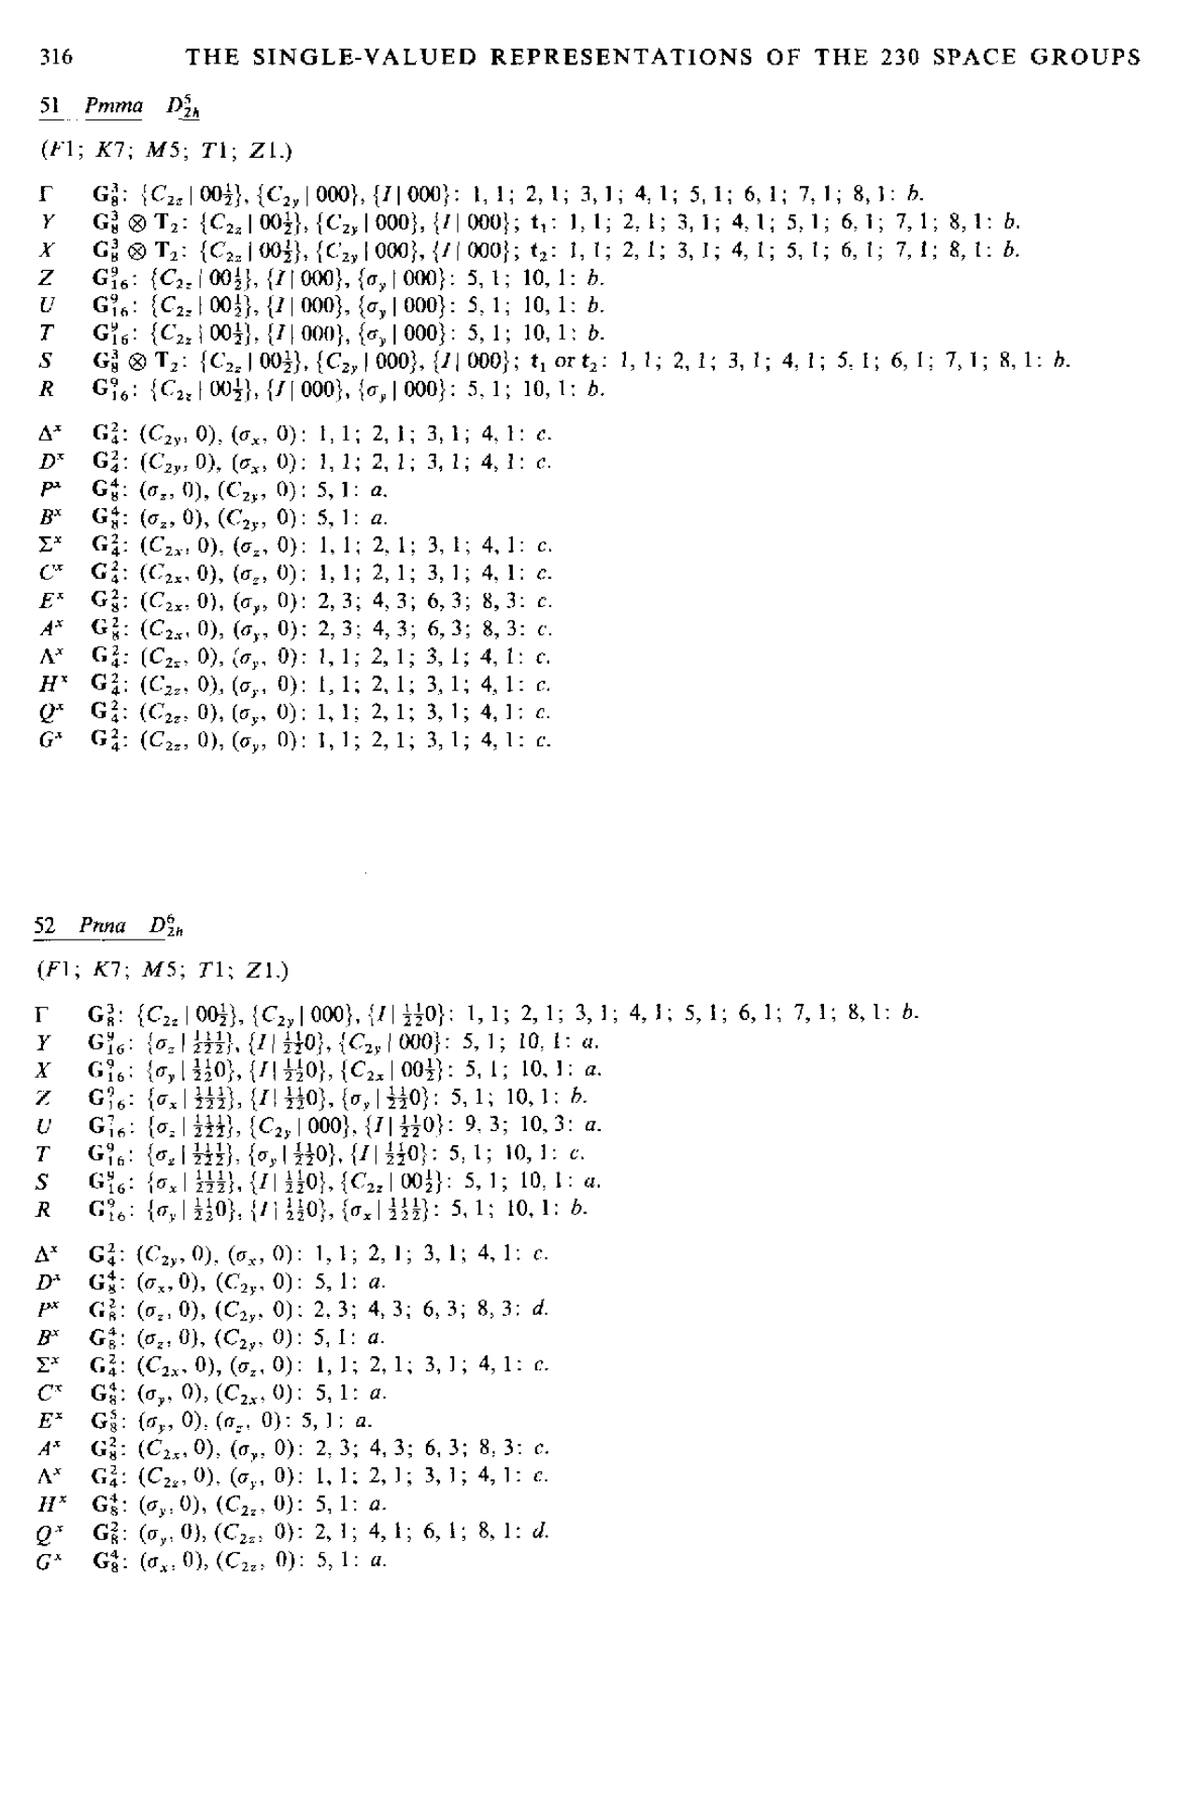
\includegraphics[width=0.86\textwidth]{c5_52_p329.jpg}
\caption*{原书第 316 页}
\end{figure}
\begin{figure}[H]
\centering
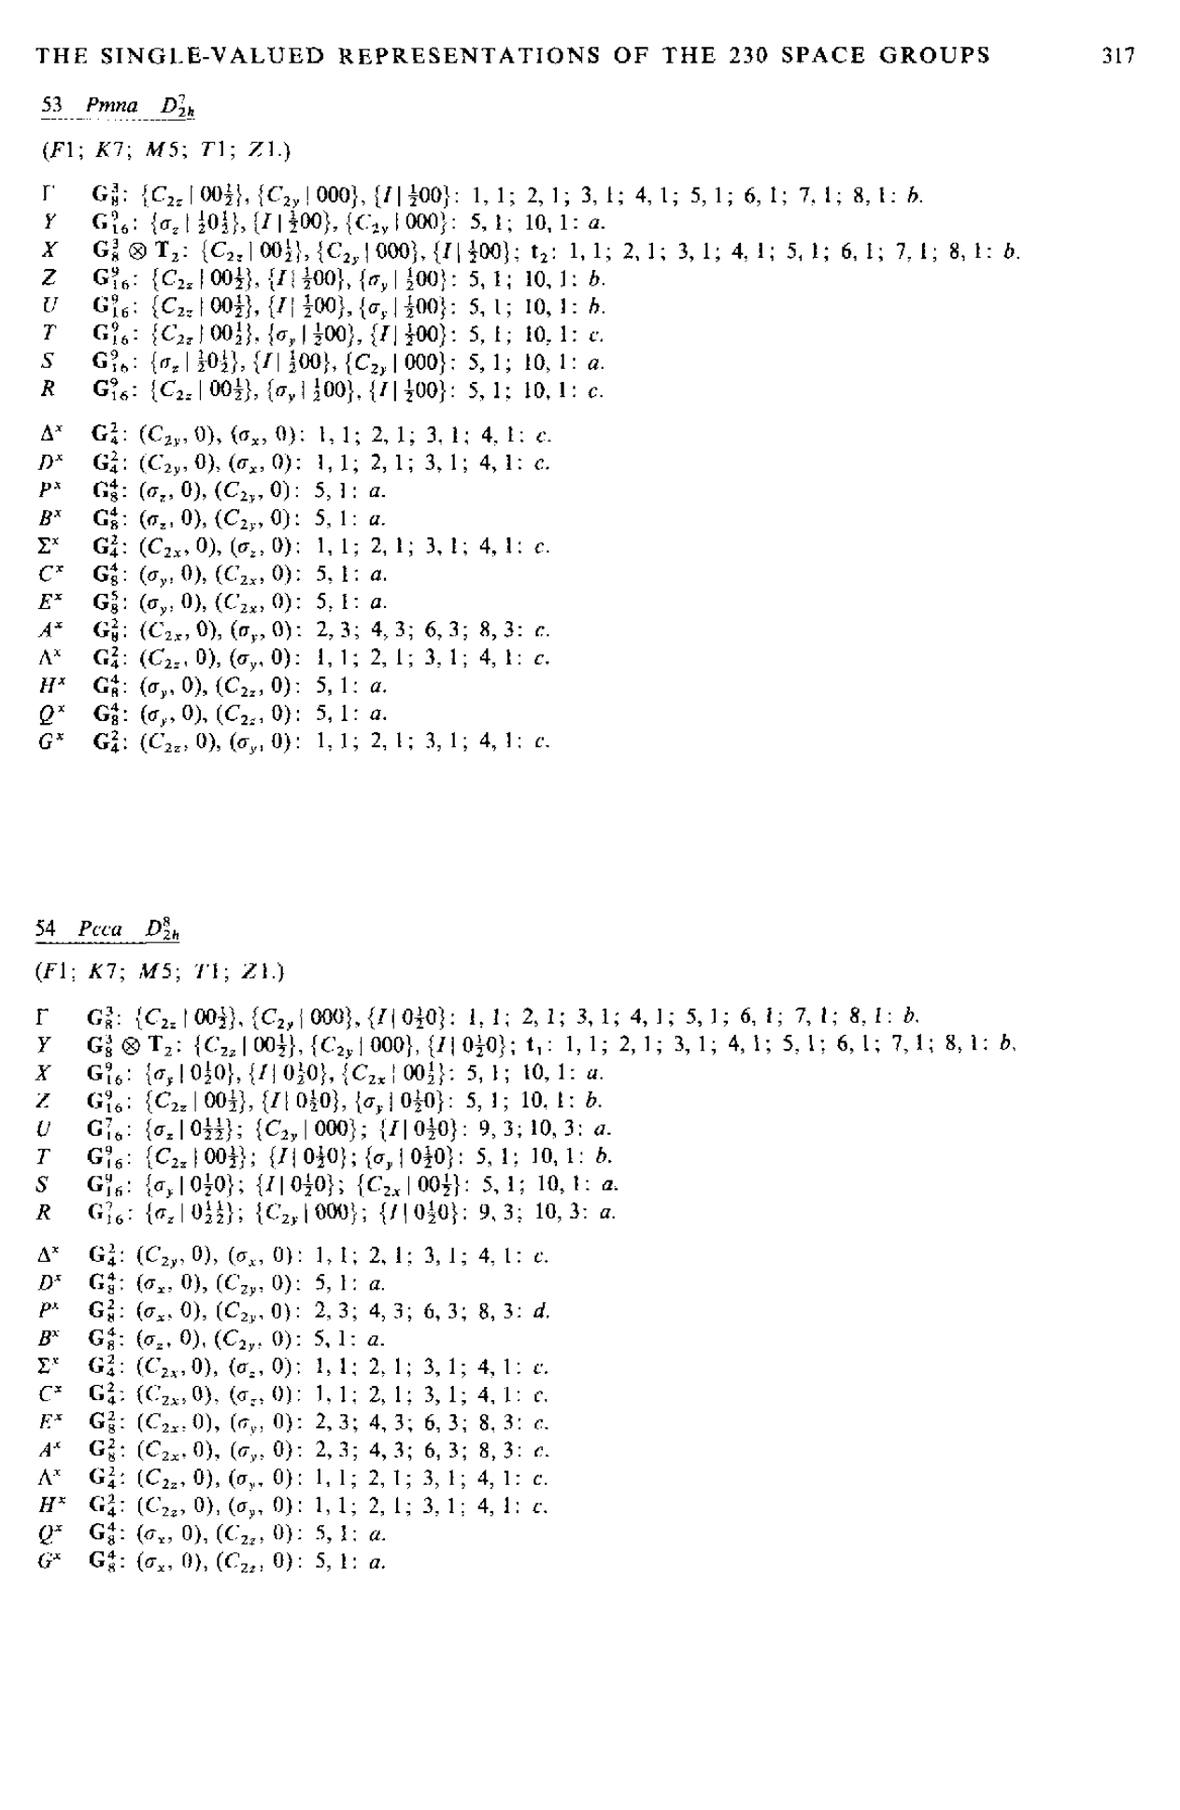
\includegraphics[width=0.86\textwidth]{c5_52_p330.jpg}
\caption*{原书第 317 页}
\end{figure}
\begin{figure}[H]
\centering
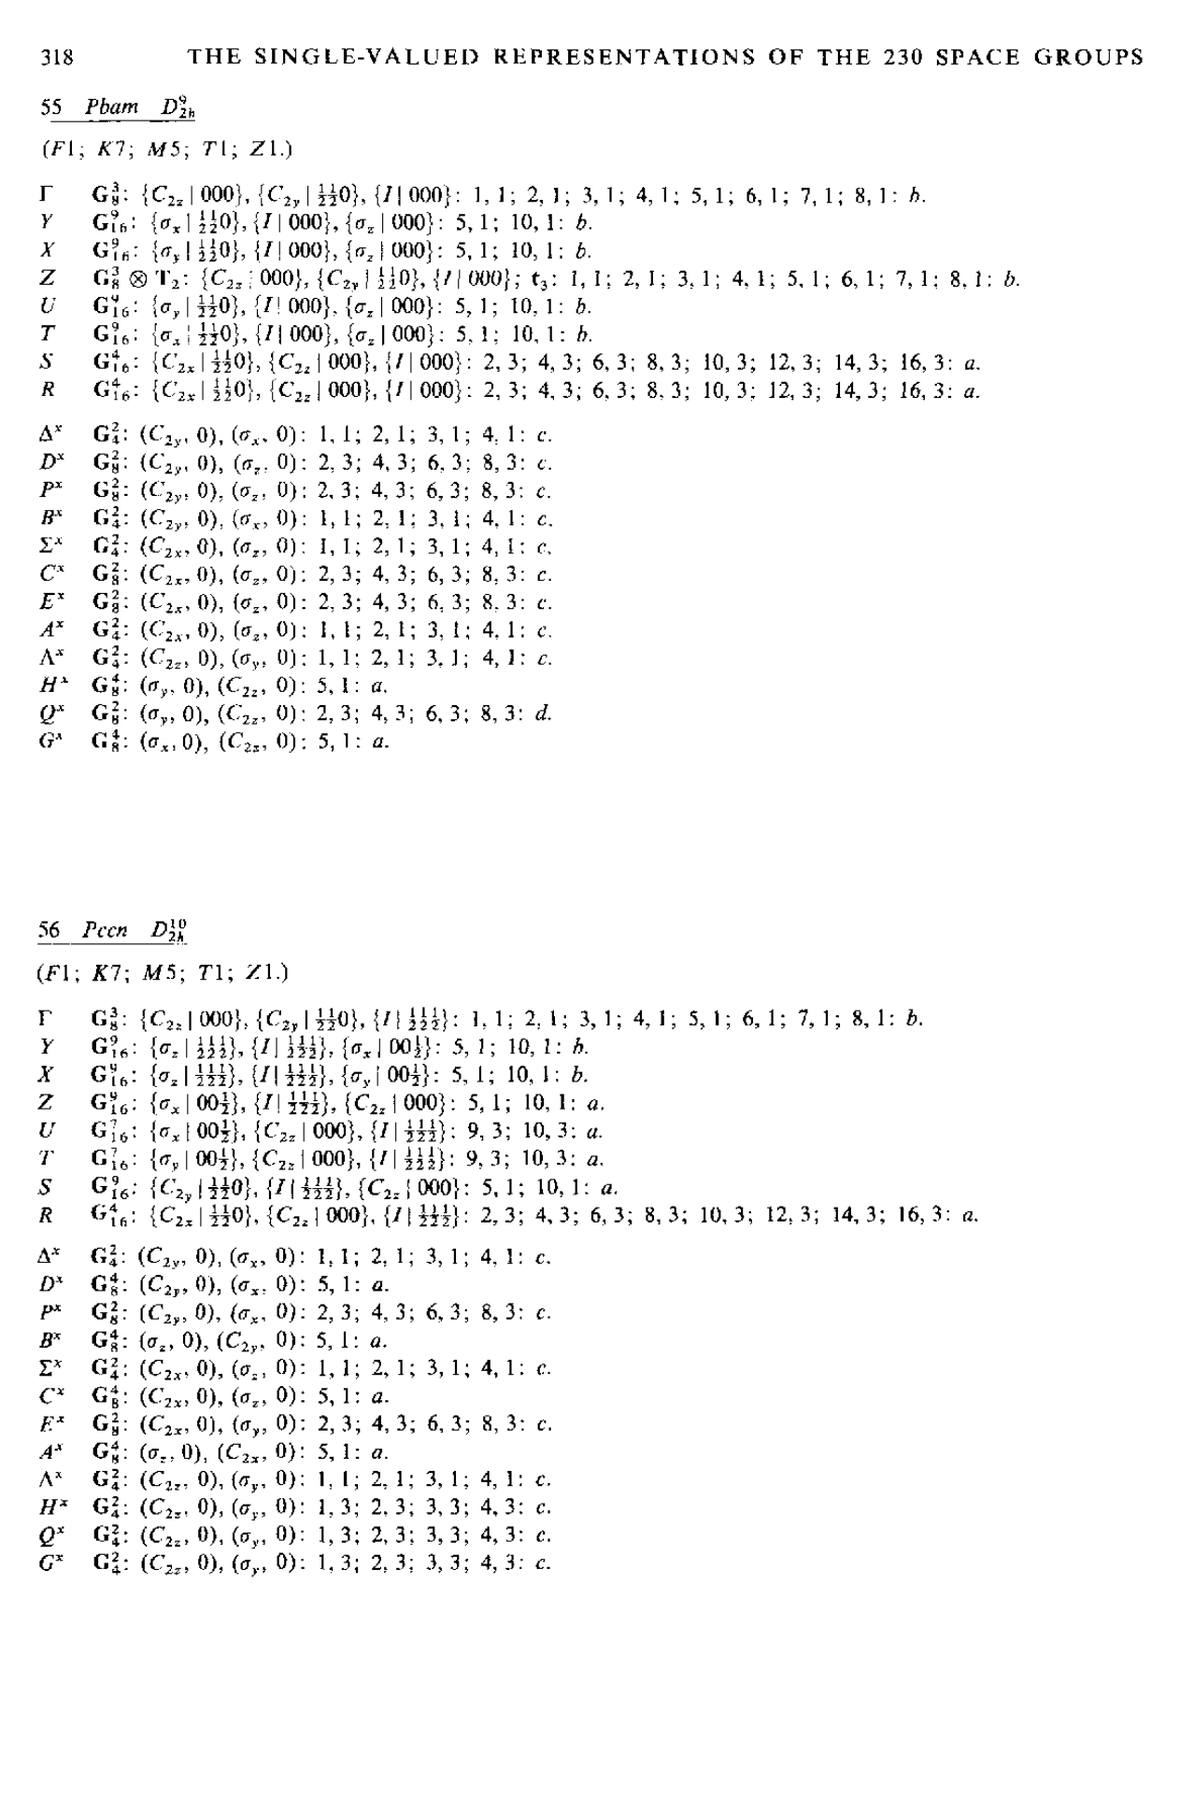
\includegraphics[width=0.86\textwidth]{c5_52_p331.jpg}
\caption*{原书第 318 页}
\end{figure}
\begin{figure}[H]
\centering
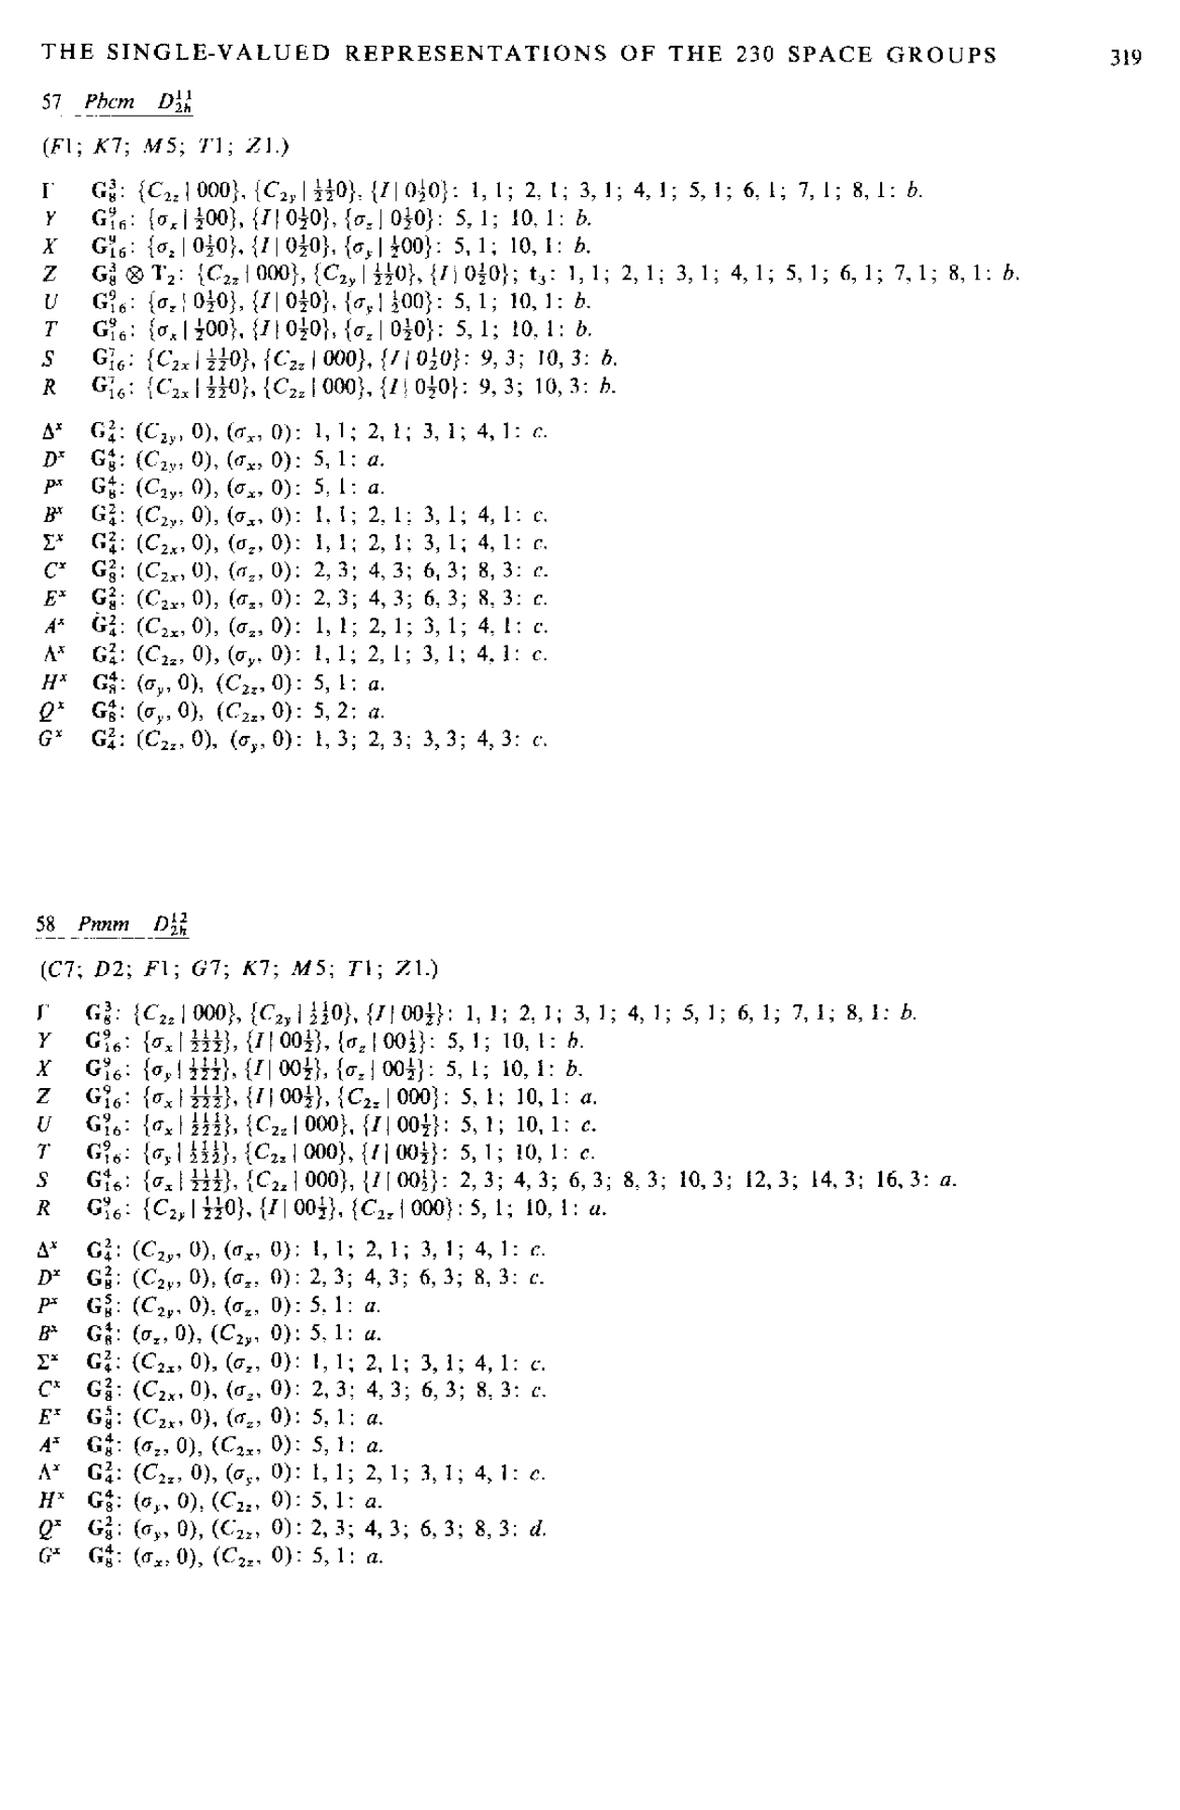
\includegraphics[width=0.86\textwidth]{c5_52_p332.jpg}
\caption*{原书第 319 页}
\end{figure}
\begin{figure}[H]
\centering
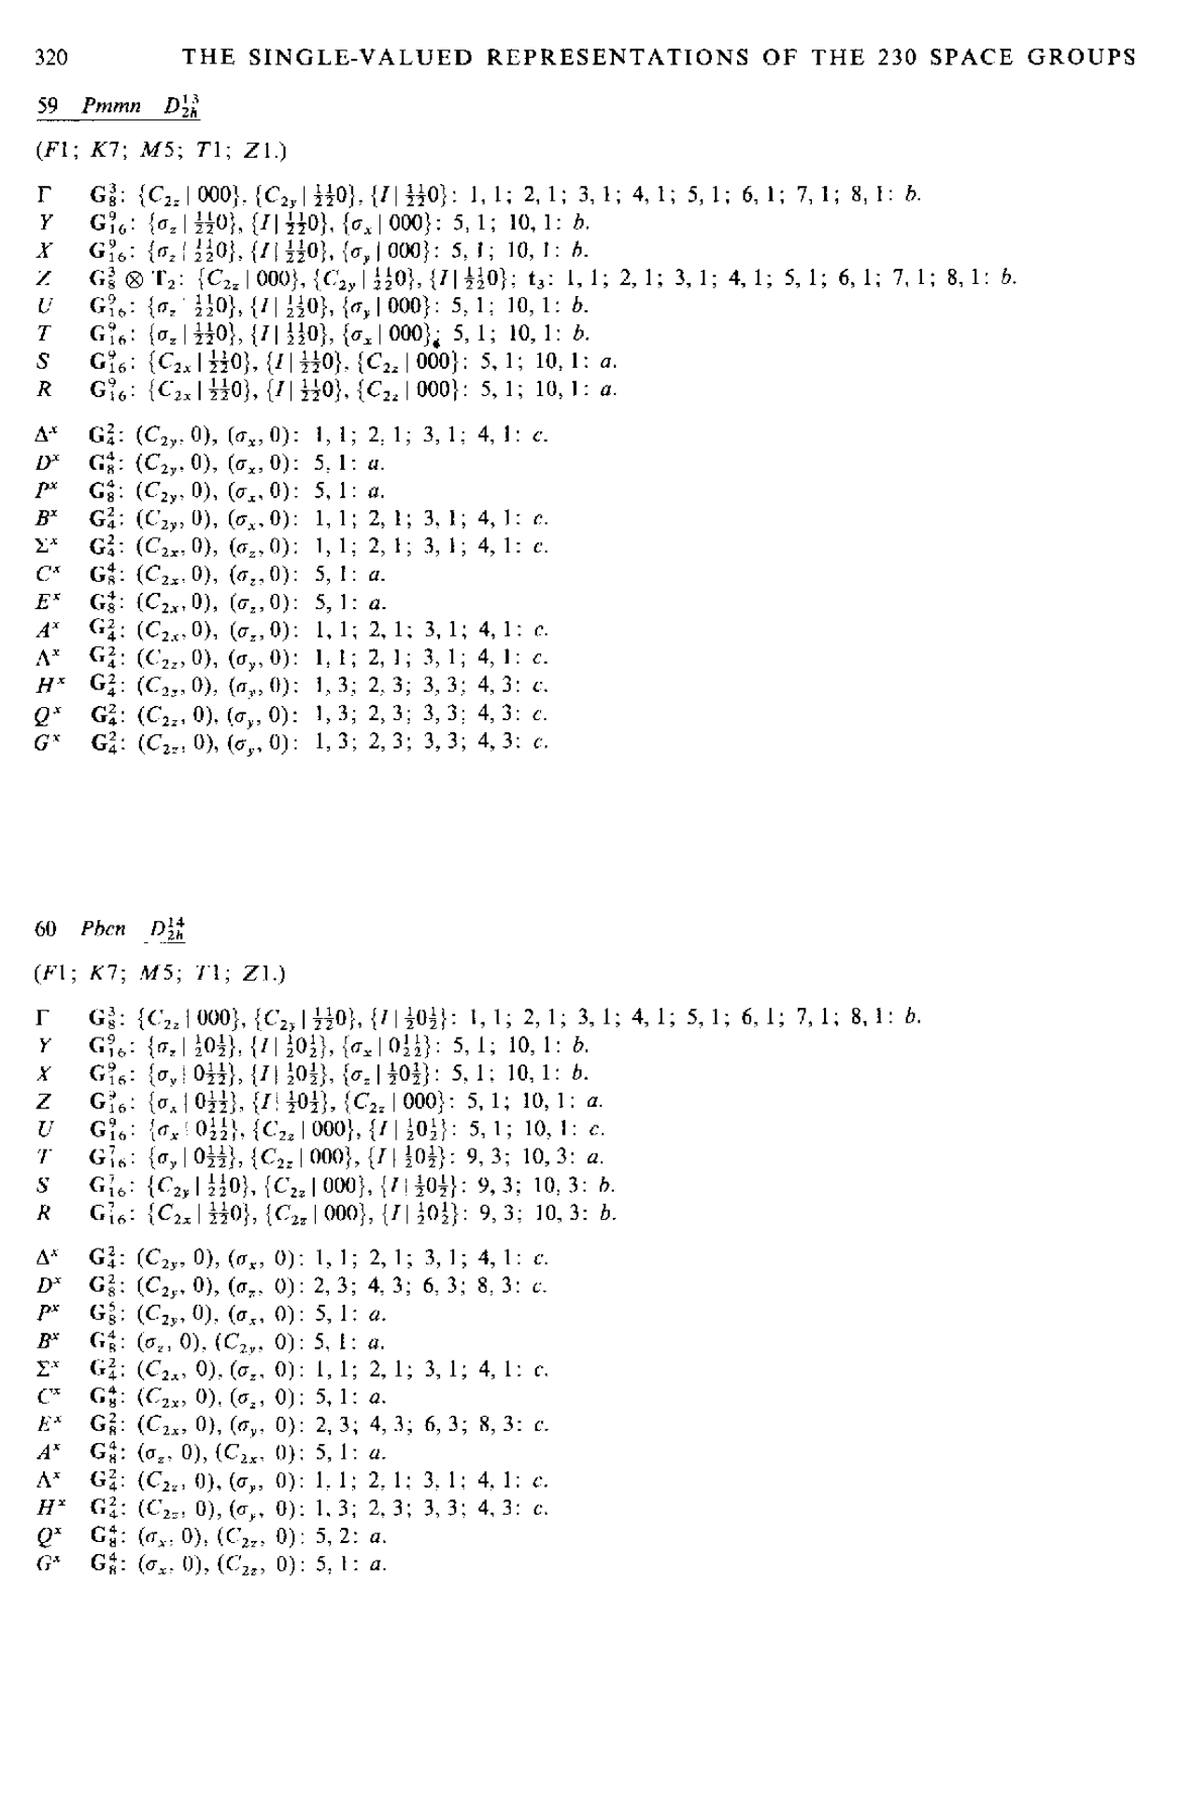
\includegraphics[width=0.86\textwidth]{c5_52_p333.jpg}
\caption*{原书第 320 页}
\end{figure}
\begin{figure}[H]
\centering
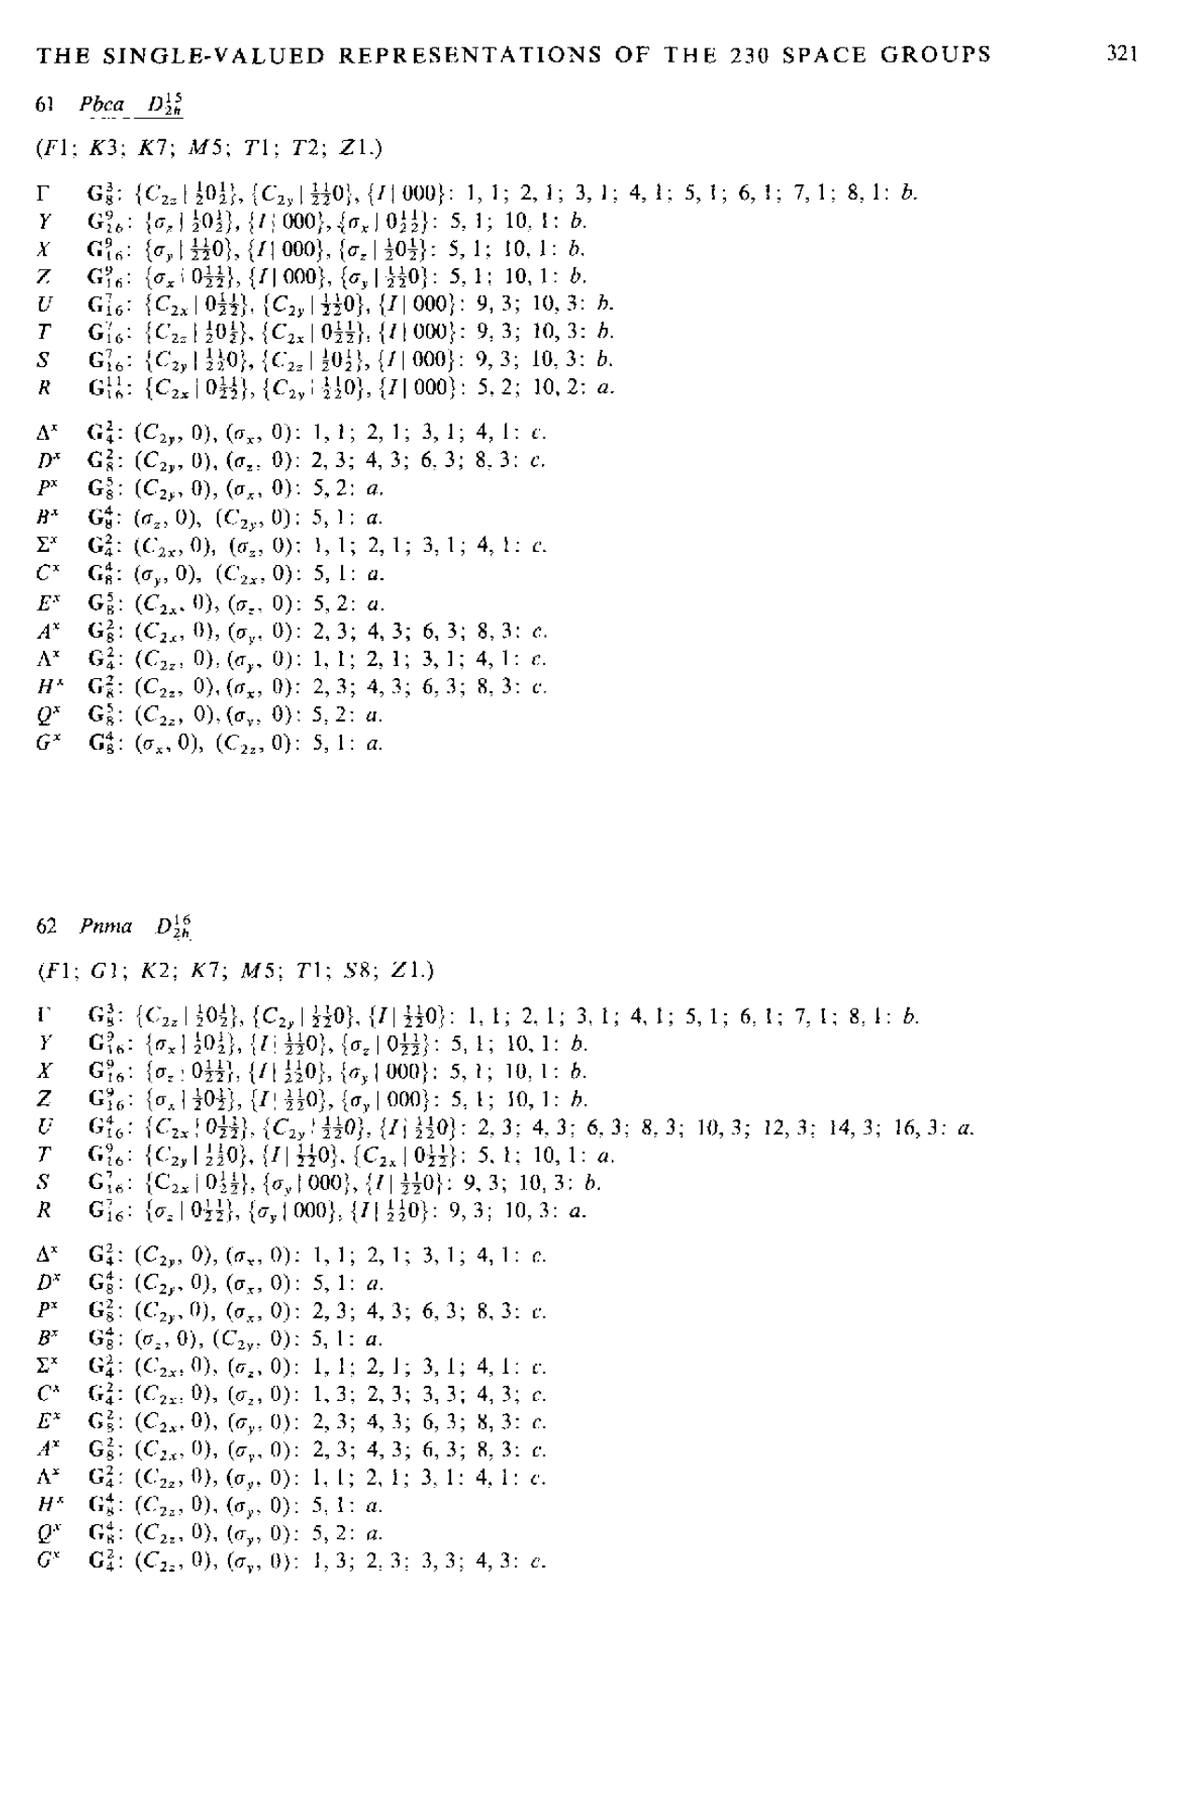
\includegraphics[width=0.86\textwidth]{c5_52_p334.jpg}
\caption*{原书第 321 页}
\end{figure}
\begin{figure}[H]
\centering
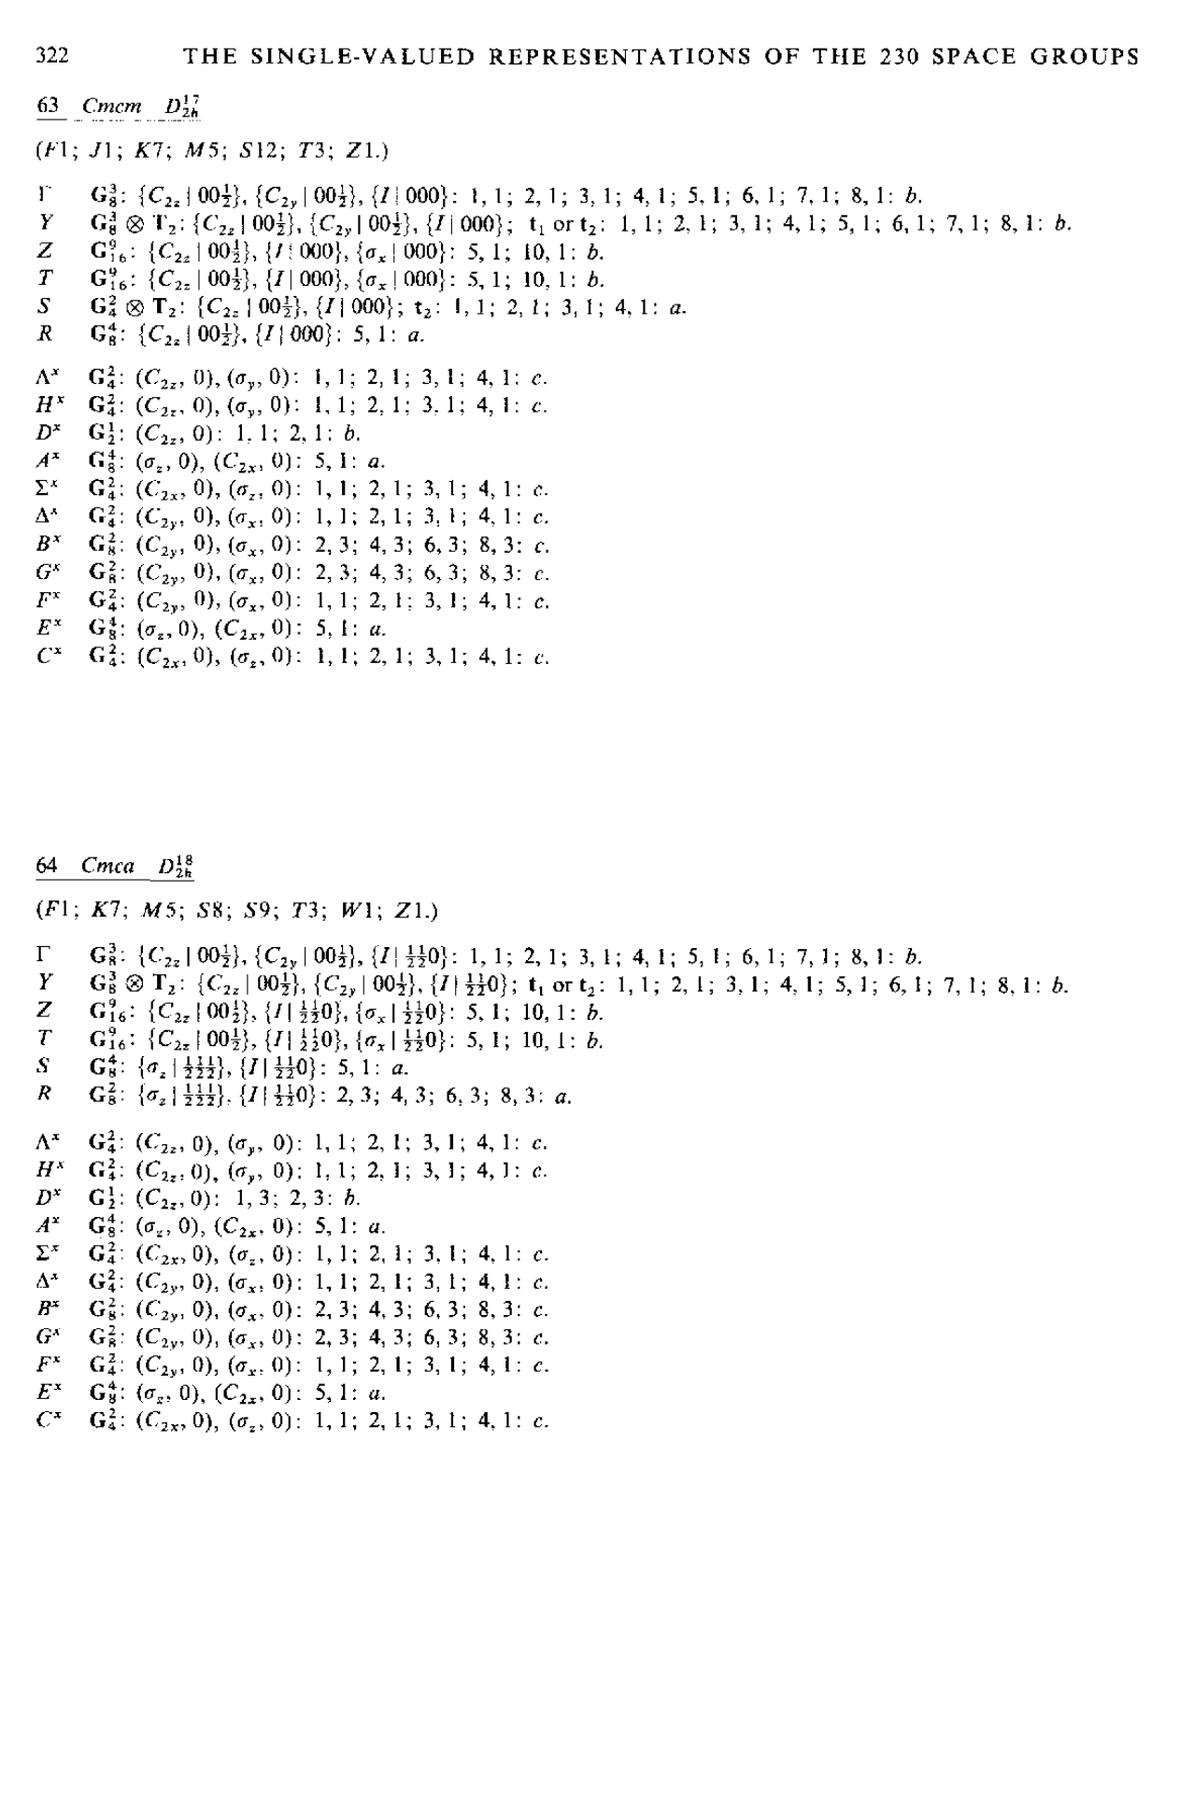
\includegraphics[width=0.86\textwidth]{c5_52_p335.jpg}
\caption*{原书第 322 页}
\end{figure}
\begin{figure}[H]
\centering
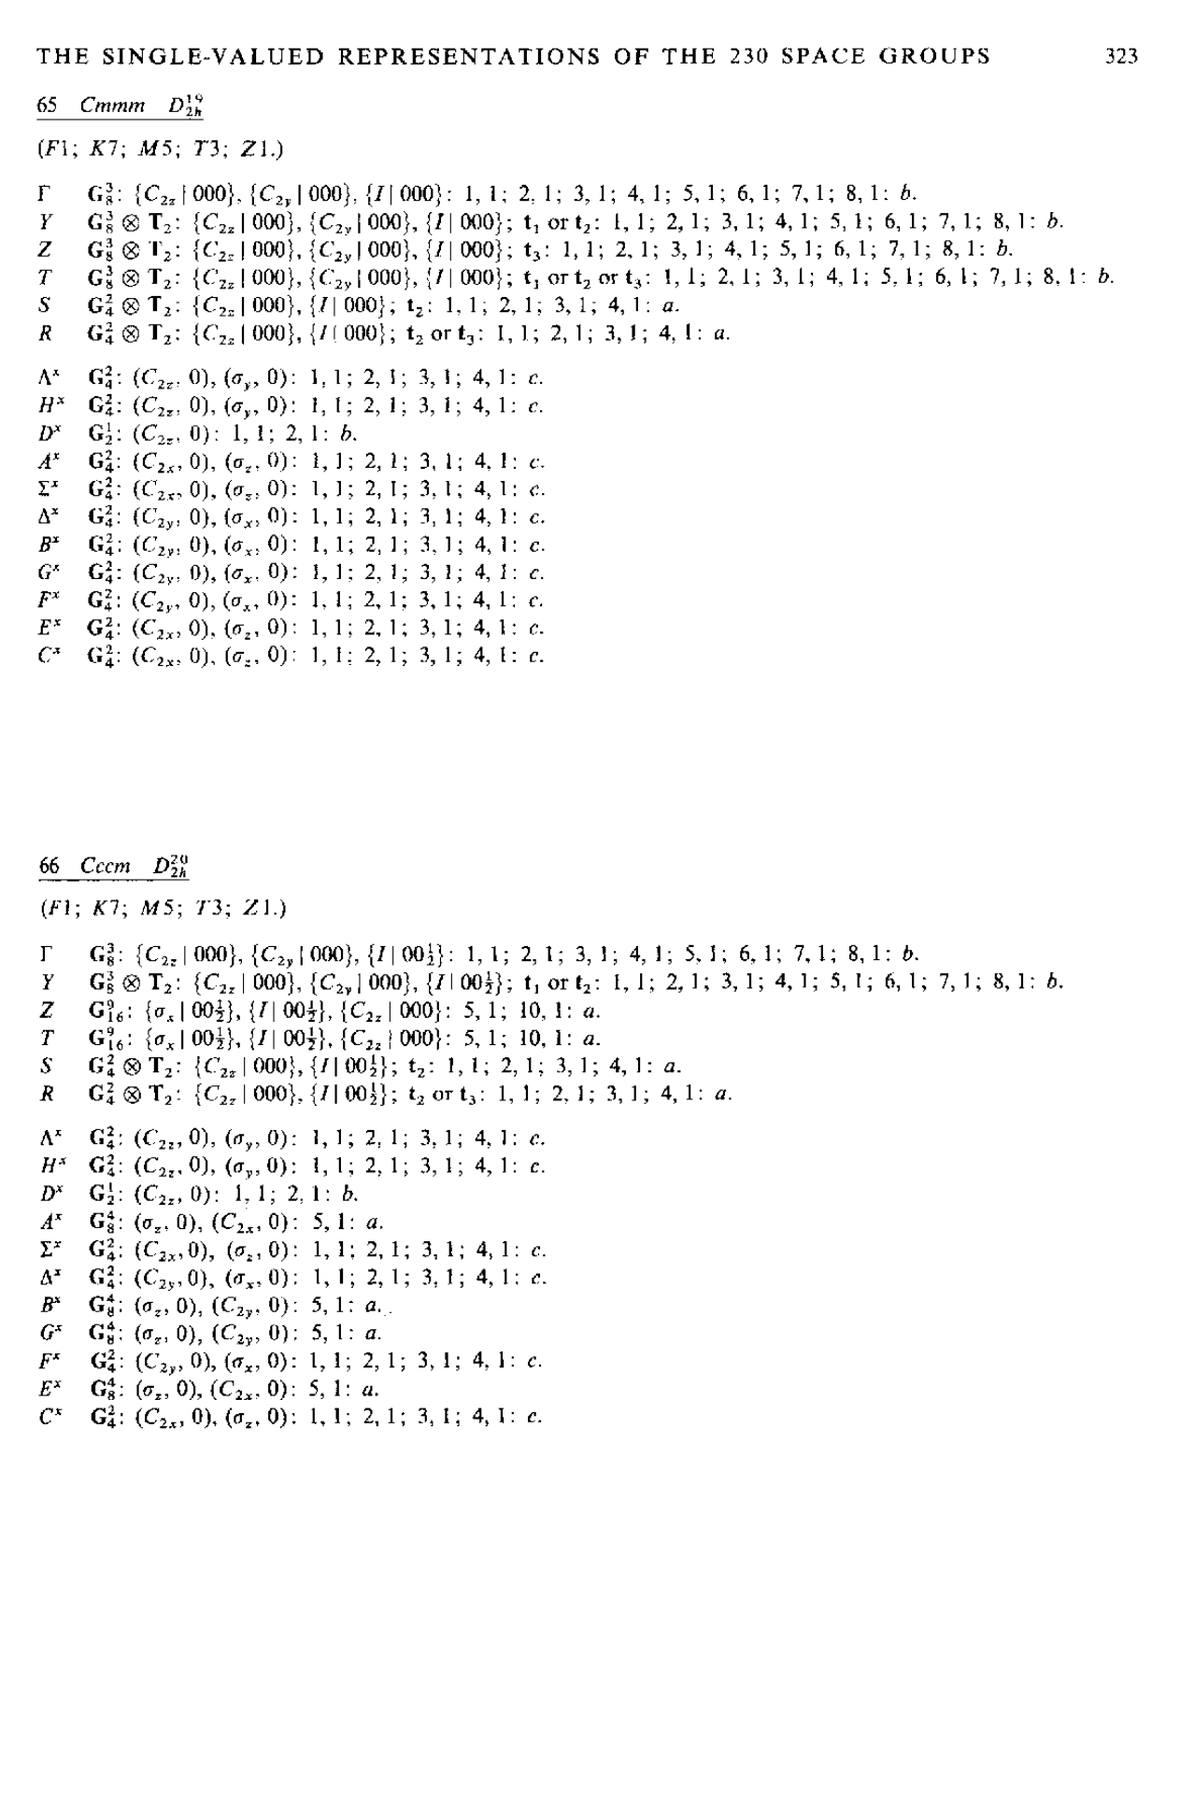
\includegraphics[width=0.86\textwidth]{c5_52_p336.jpg}
\caption*{原书第 323 页}
\end{figure}
\begin{figure}[H]
\centering
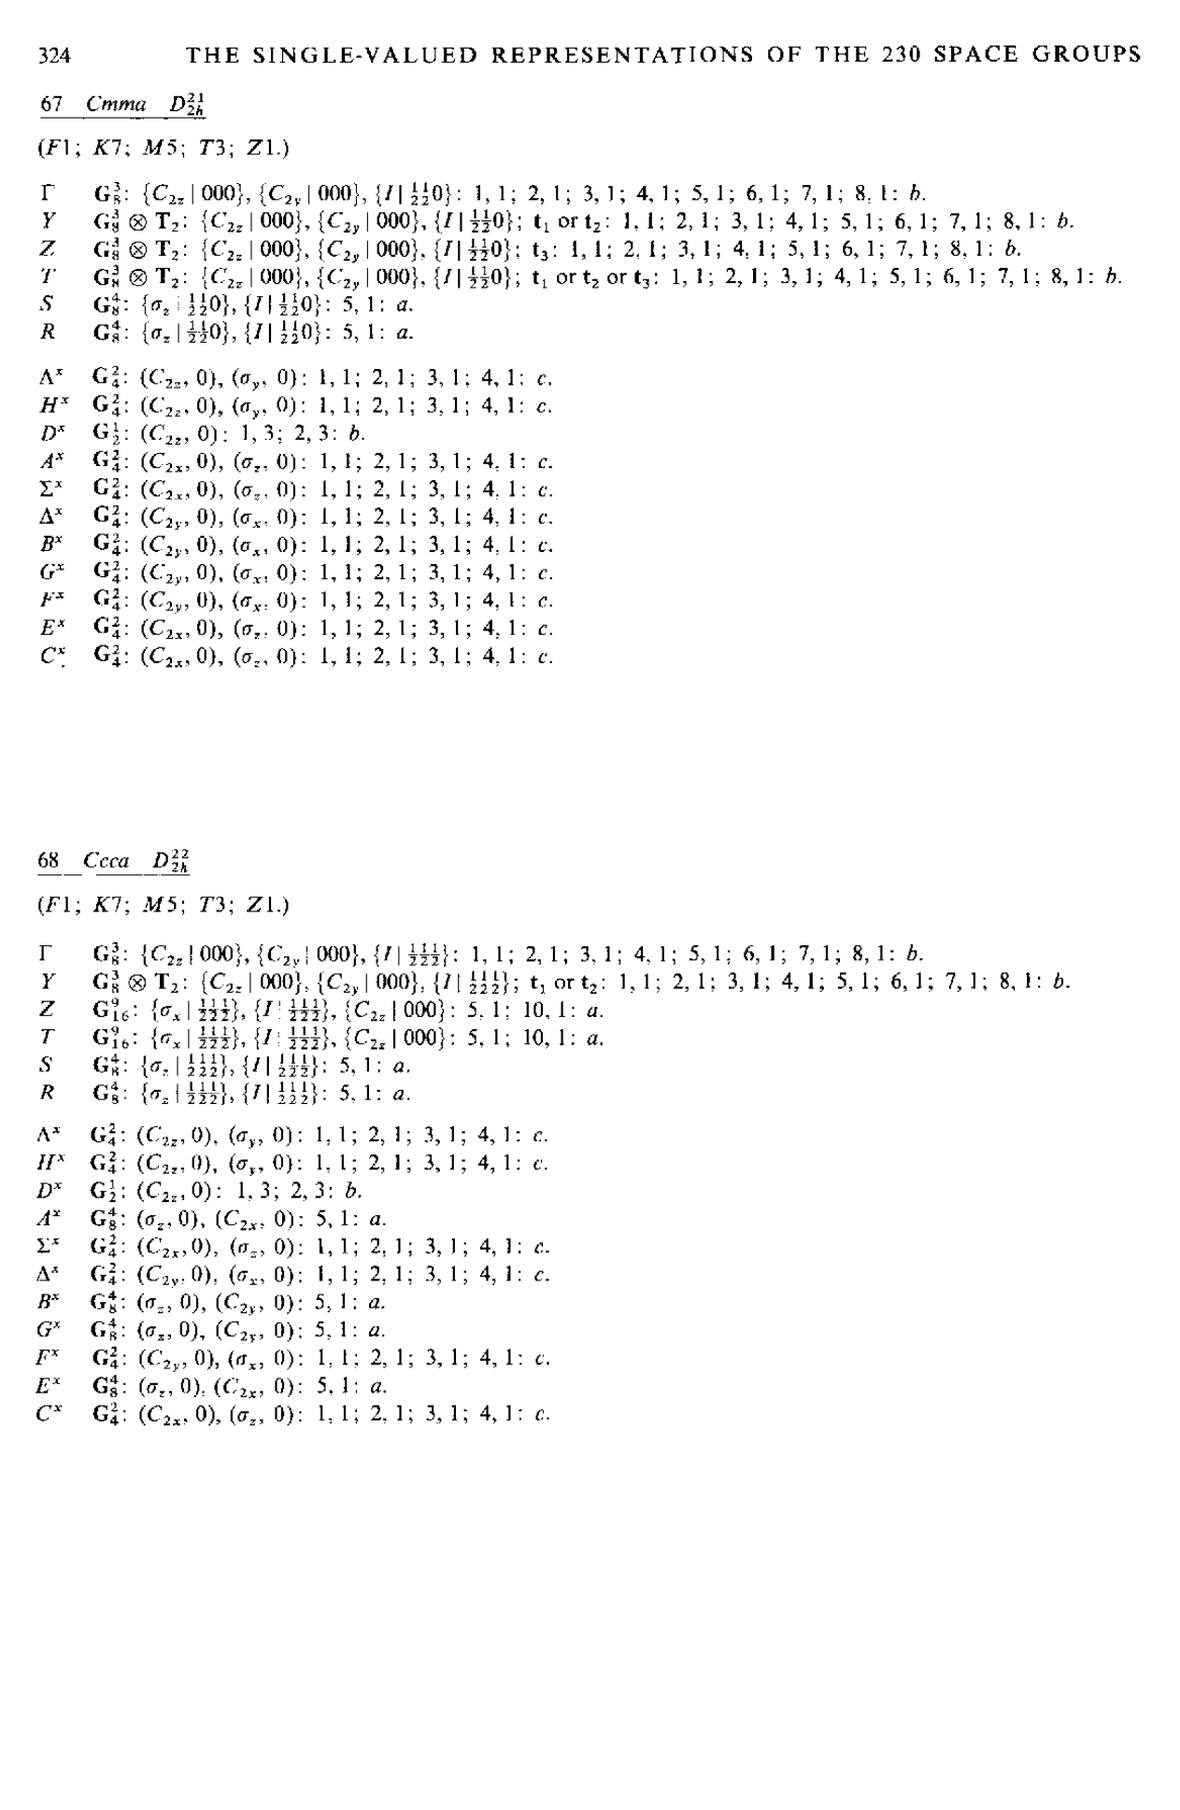
\includegraphics[width=0.86\textwidth]{c5_52_p337.jpg}
\caption*{原书第 324 页}
\end{figure}
\begin{figure}[H]
\centering
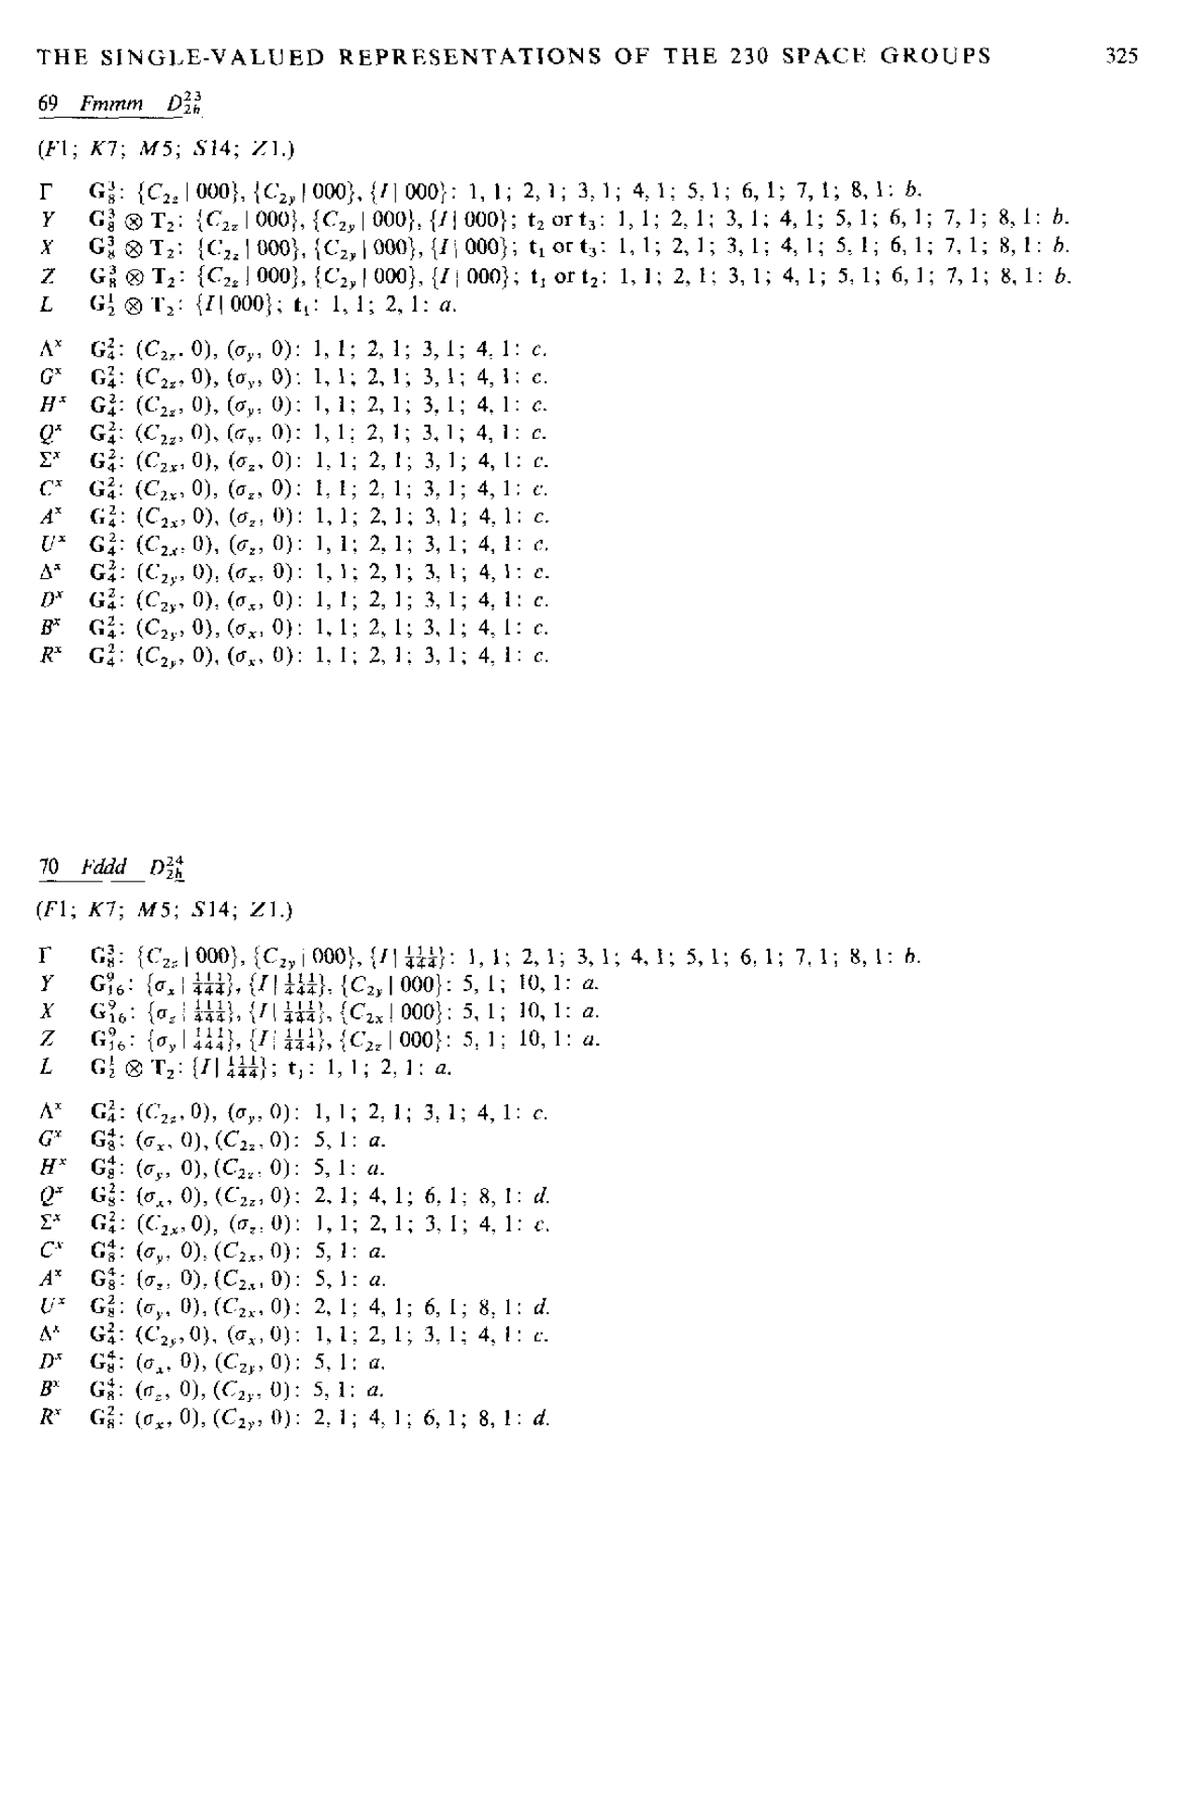
\includegraphics[width=0.86\textwidth]{c5_52_p338.jpg}
\caption*{原书第 325 页}
\end{figure}
\begin{figure}[H]
\centering
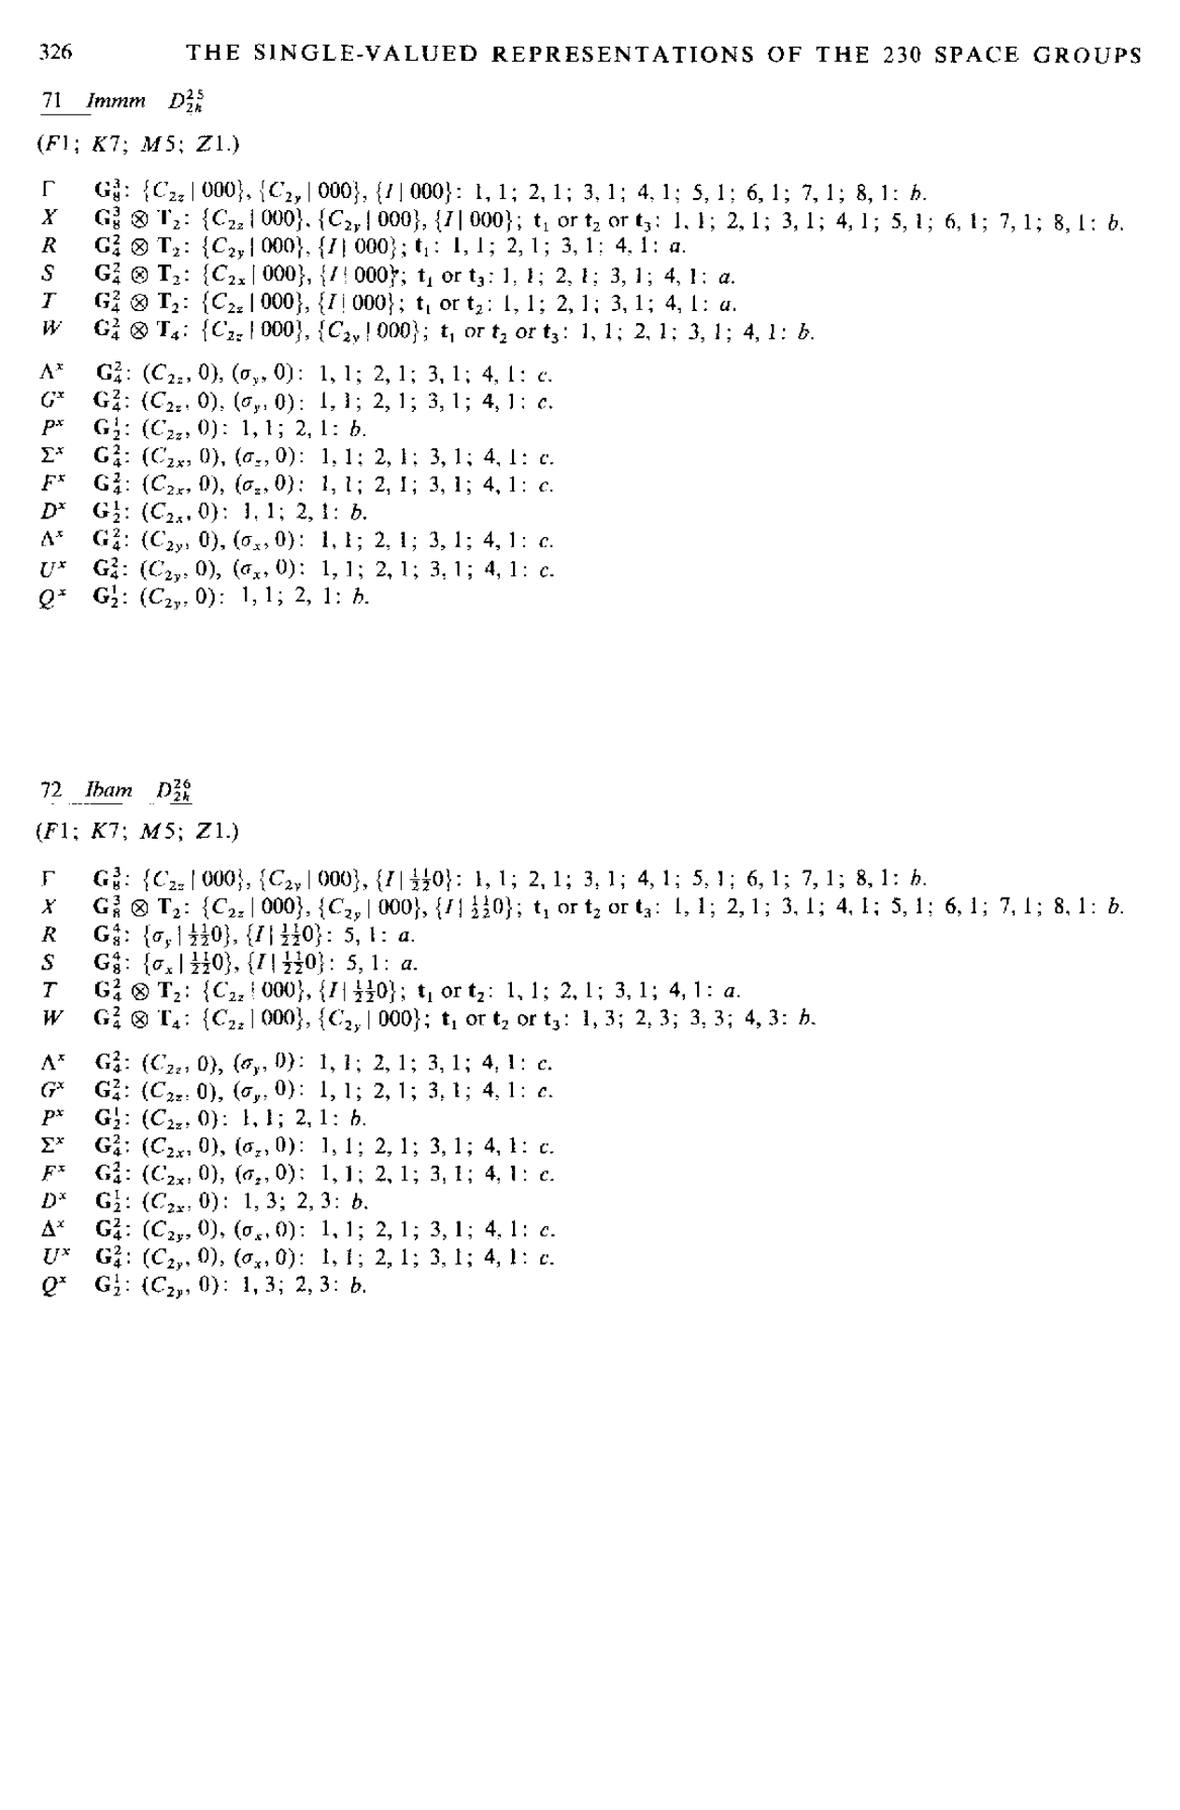
\includegraphics[width=0.86\textwidth]{c5_52_p339.jpg}
\caption*{原书第 326 页}
\end{figure}
\begin{figure}[H]
\centering
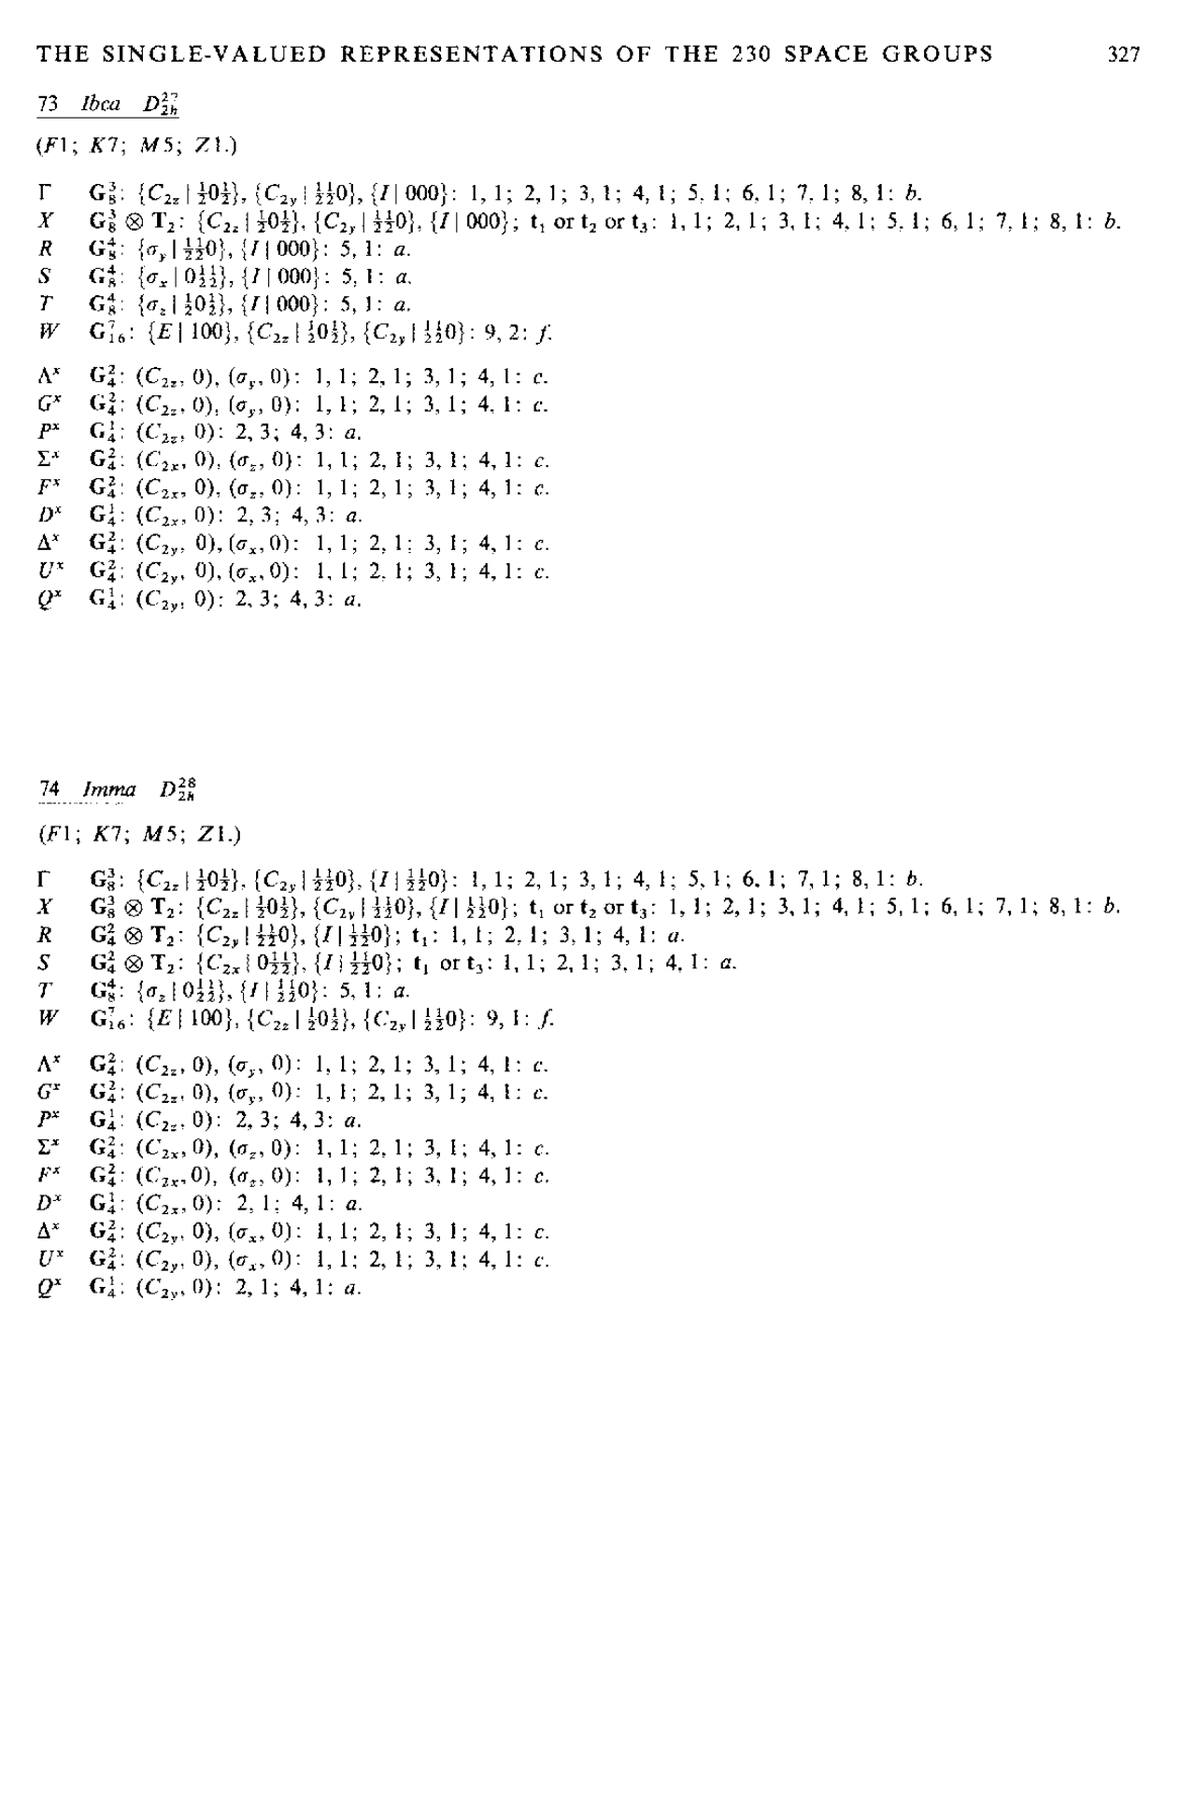
\includegraphics[width=0.86\textwidth]{c5_52_p340.jpg}
\caption*{原书第 327 页}
\end{figure}
\begin{figure}[H]
\centering
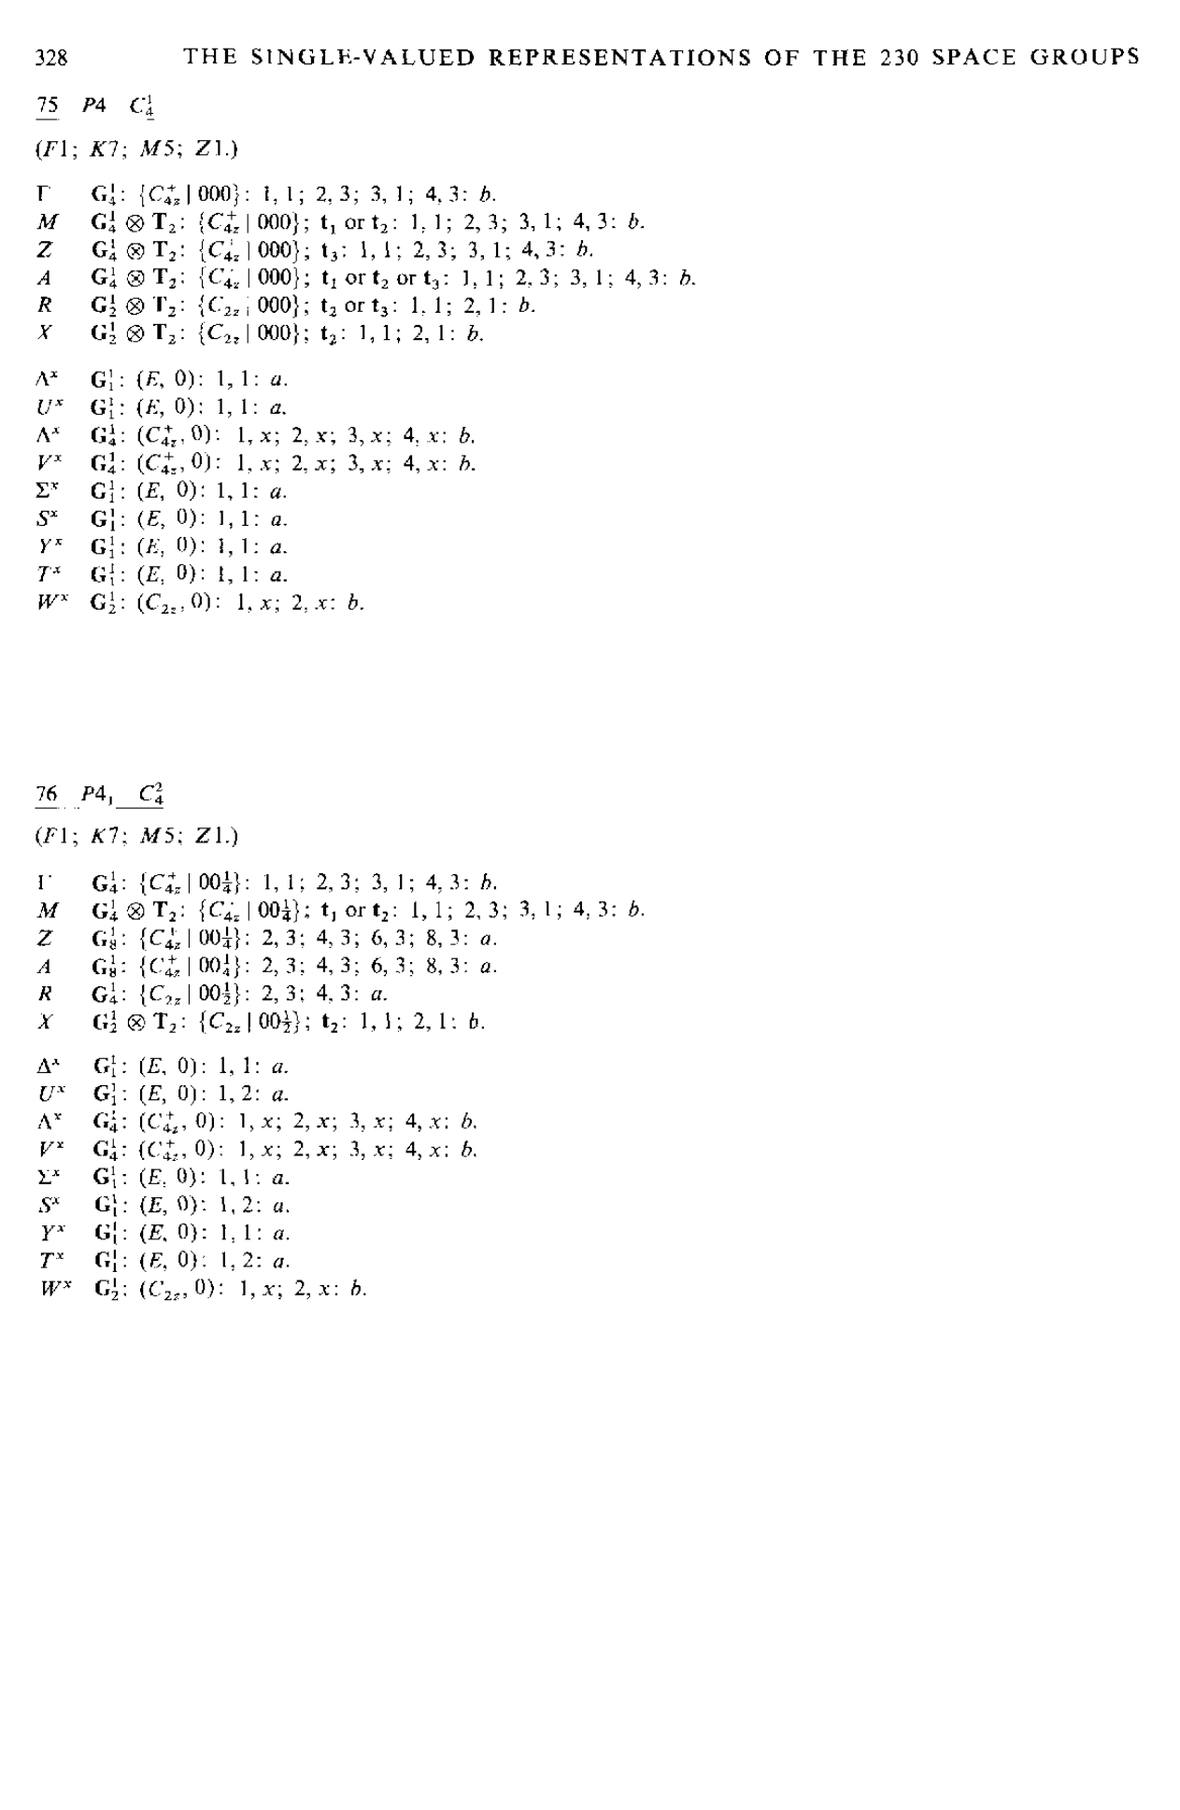
\includegraphics[width=0.86\textwidth]{c5_52_p341.jpg}
\caption*{原书第 328 页}
\end{figure}
\begin{figure}[H]
\centering
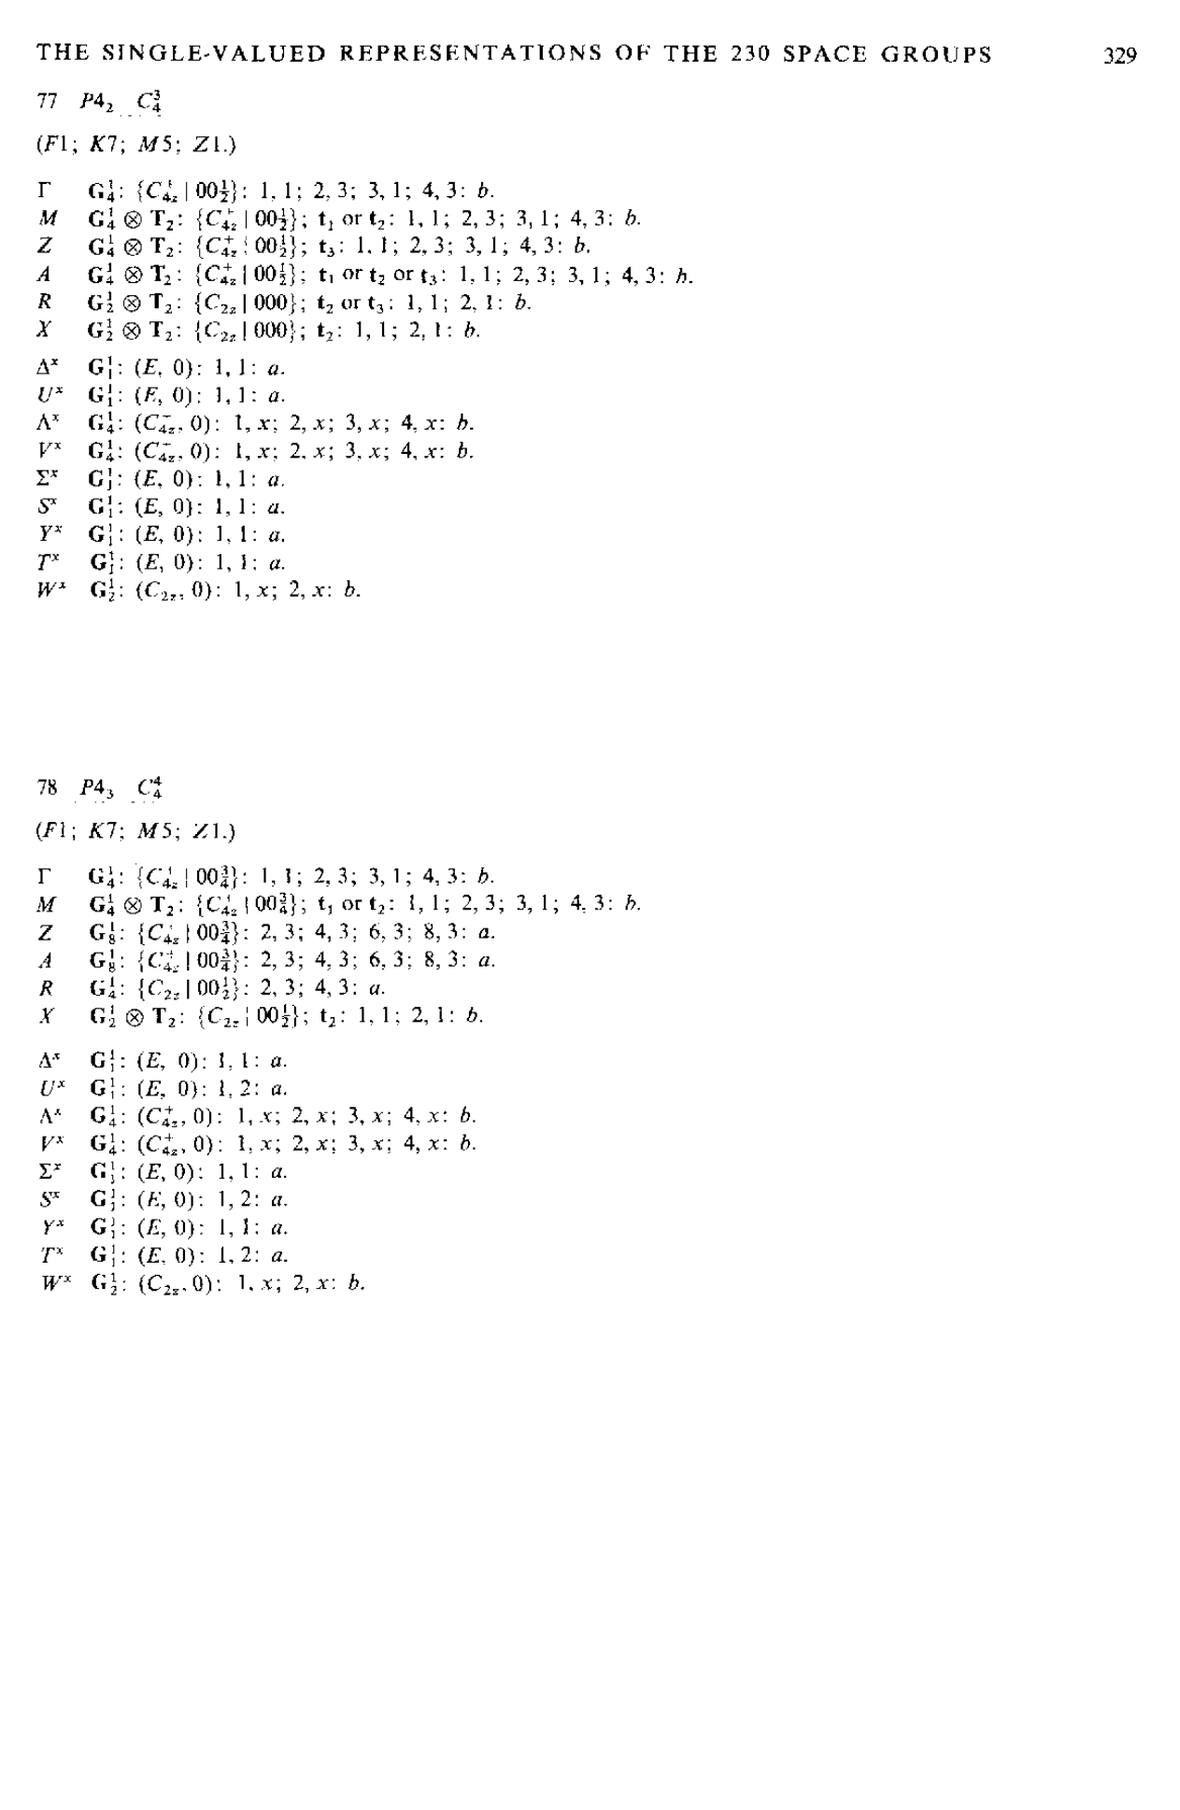
\includegraphics[width=0.86\textwidth]{c5_52_p342.jpg}
\caption*{原书第 329 页}
\end{figure}
\begin{figure}[H]
\centering
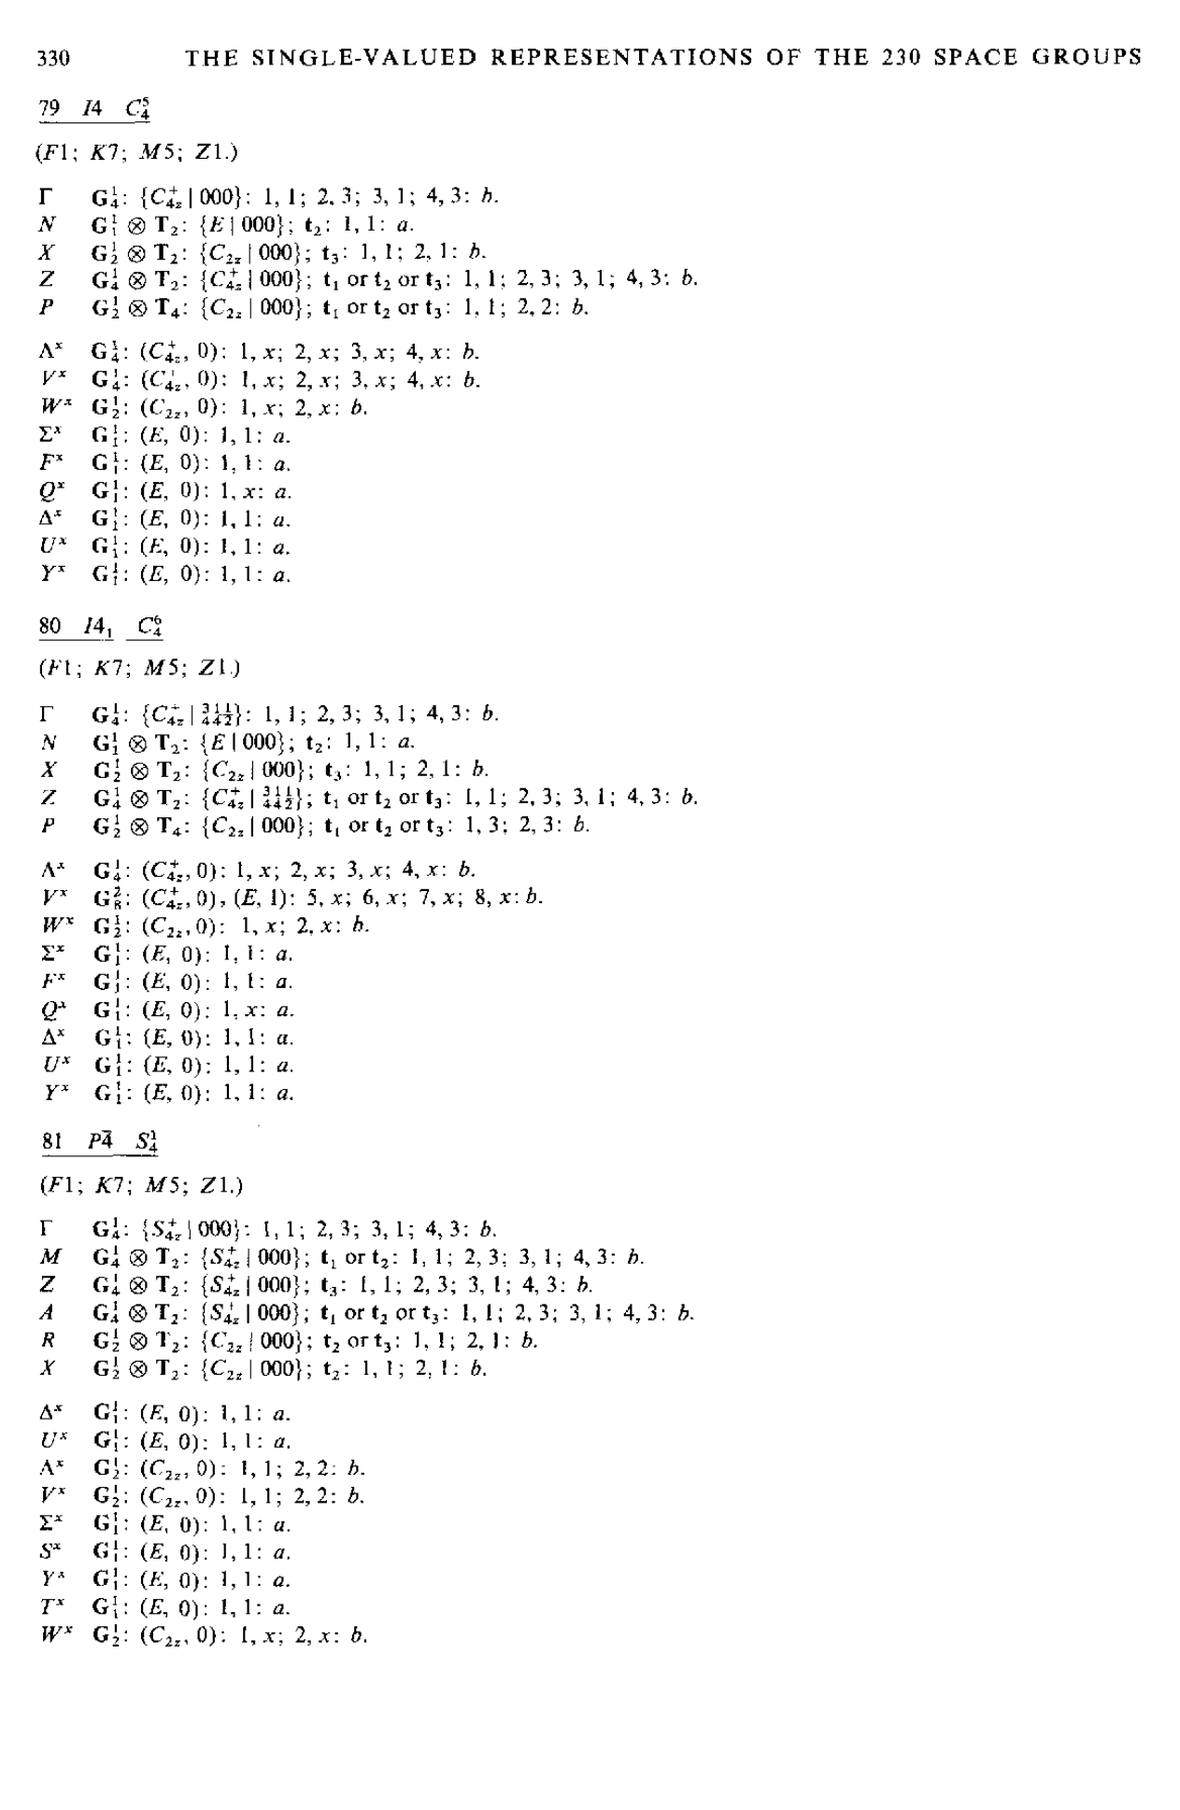
\includegraphics[width=0.86\textwidth]{c5_52_p343.jpg}
\caption*{原书第 330 页}
\end{figure}
\begin{figure}[H]
\centering
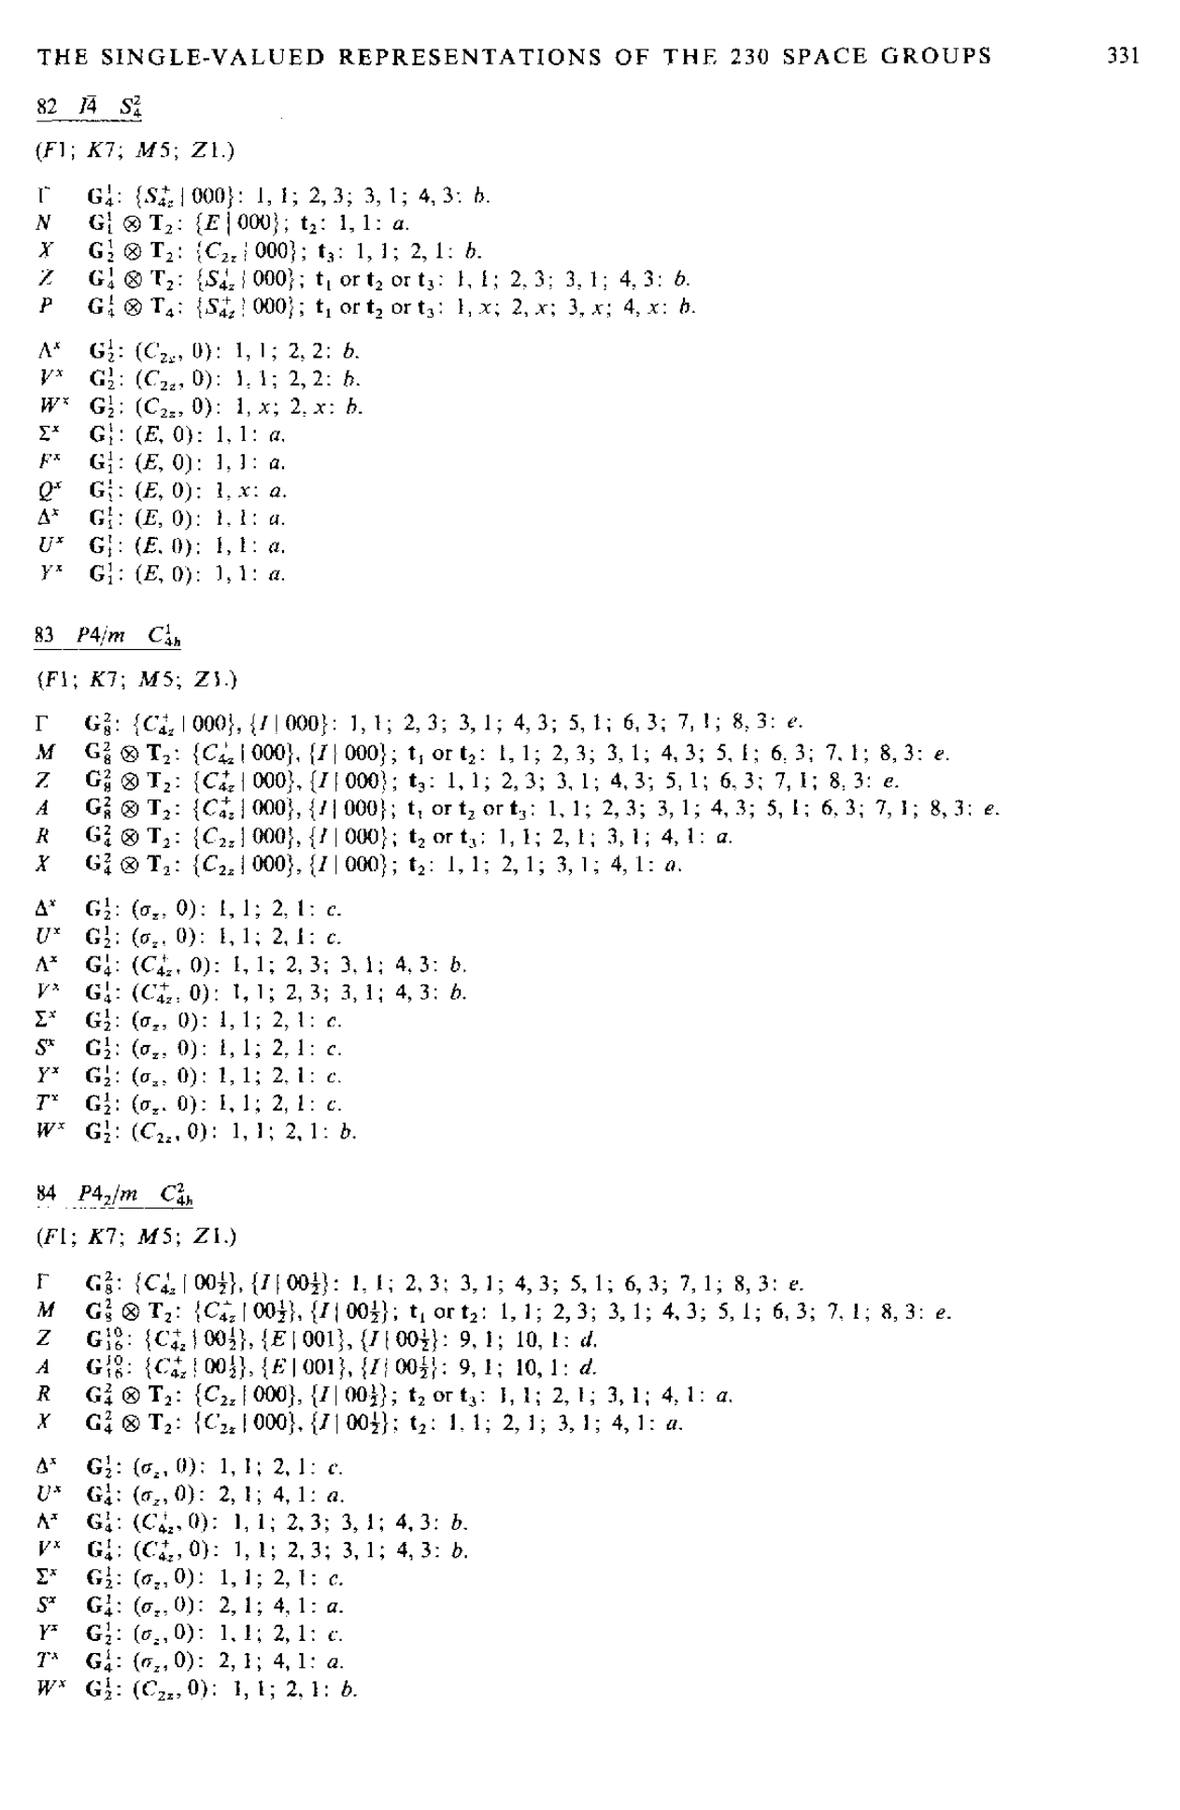
\includegraphics[width=0.86\textwidth]{c5_52_p344.jpg}
\caption*{原书第 331 页}
\end{figure}
\begin{figure}[H]
\centering
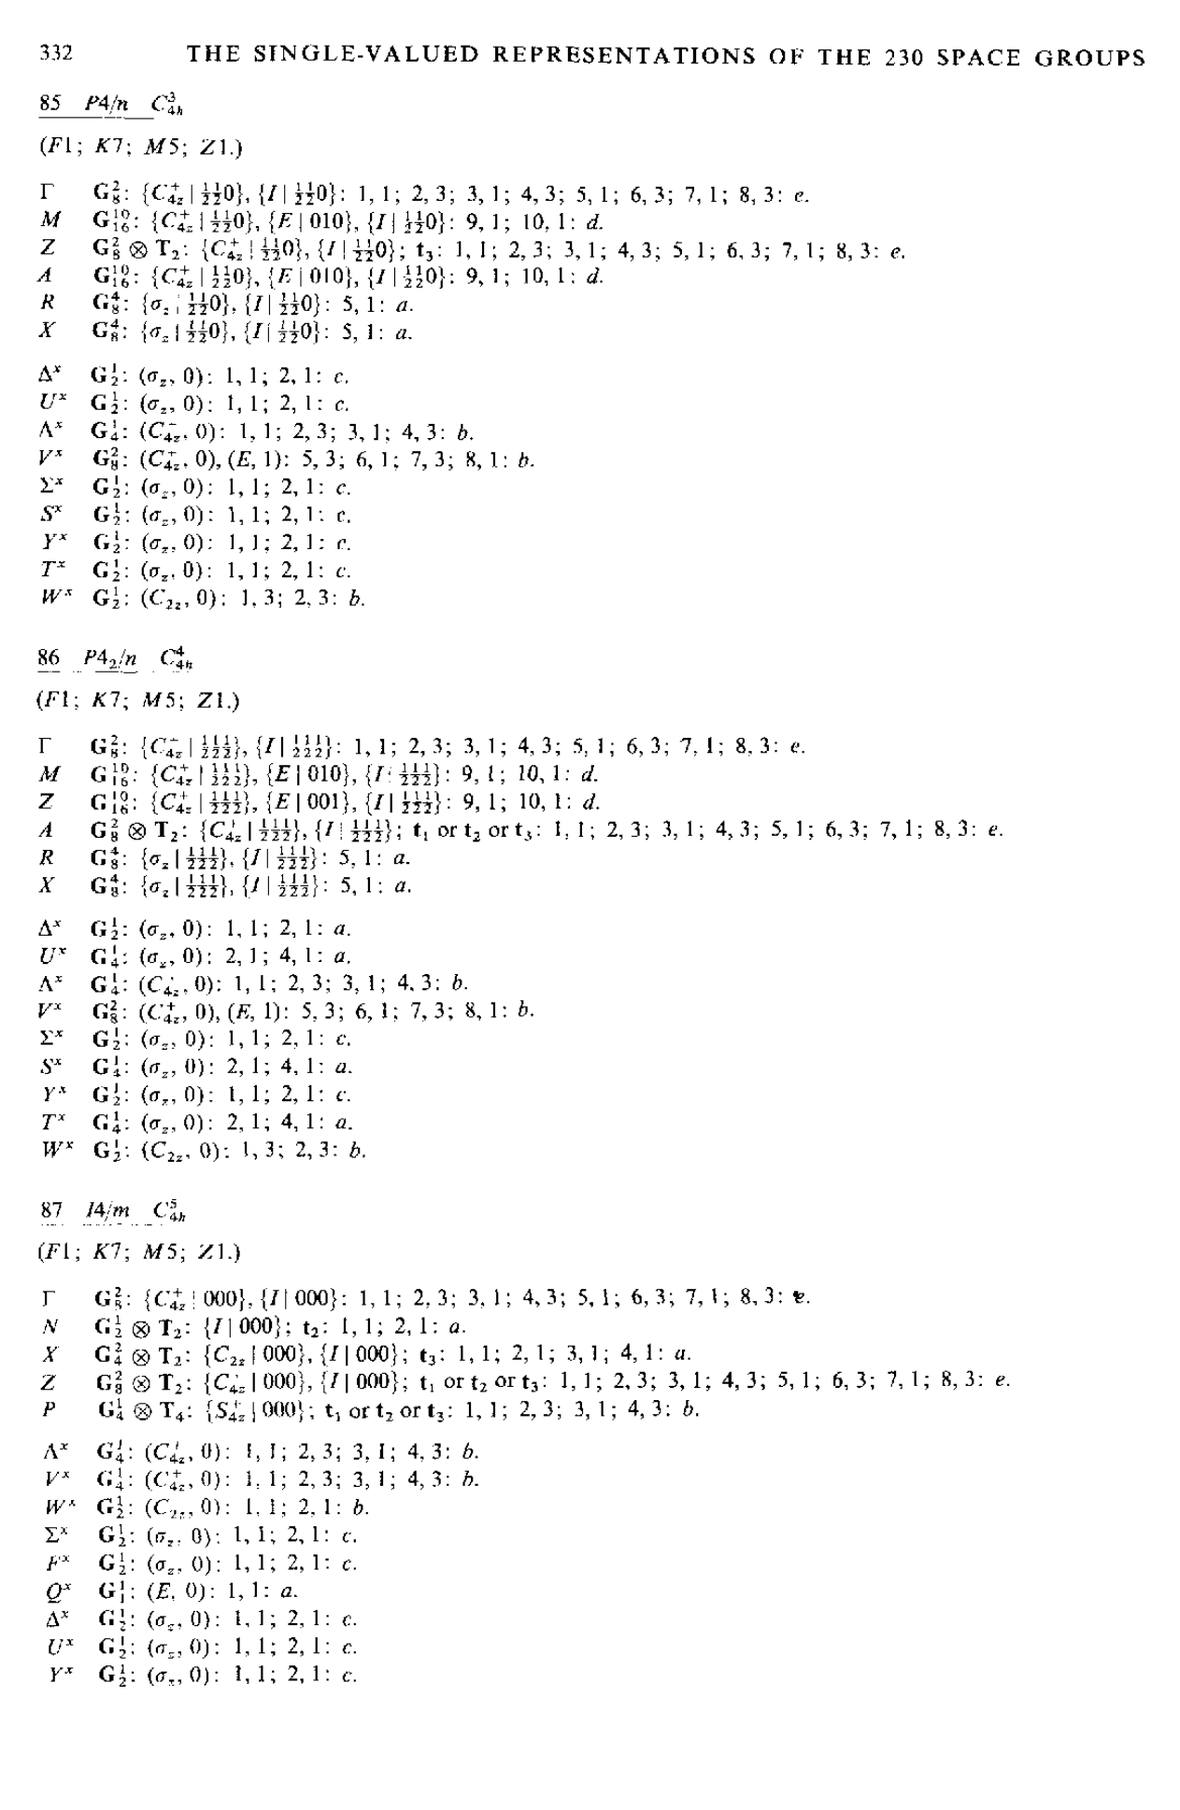
\includegraphics[width=0.86\textwidth]{c5_52_p345.jpg}
\caption*{原书第 332 页}
\end{figure}
\begin{figure}[H]
\centering
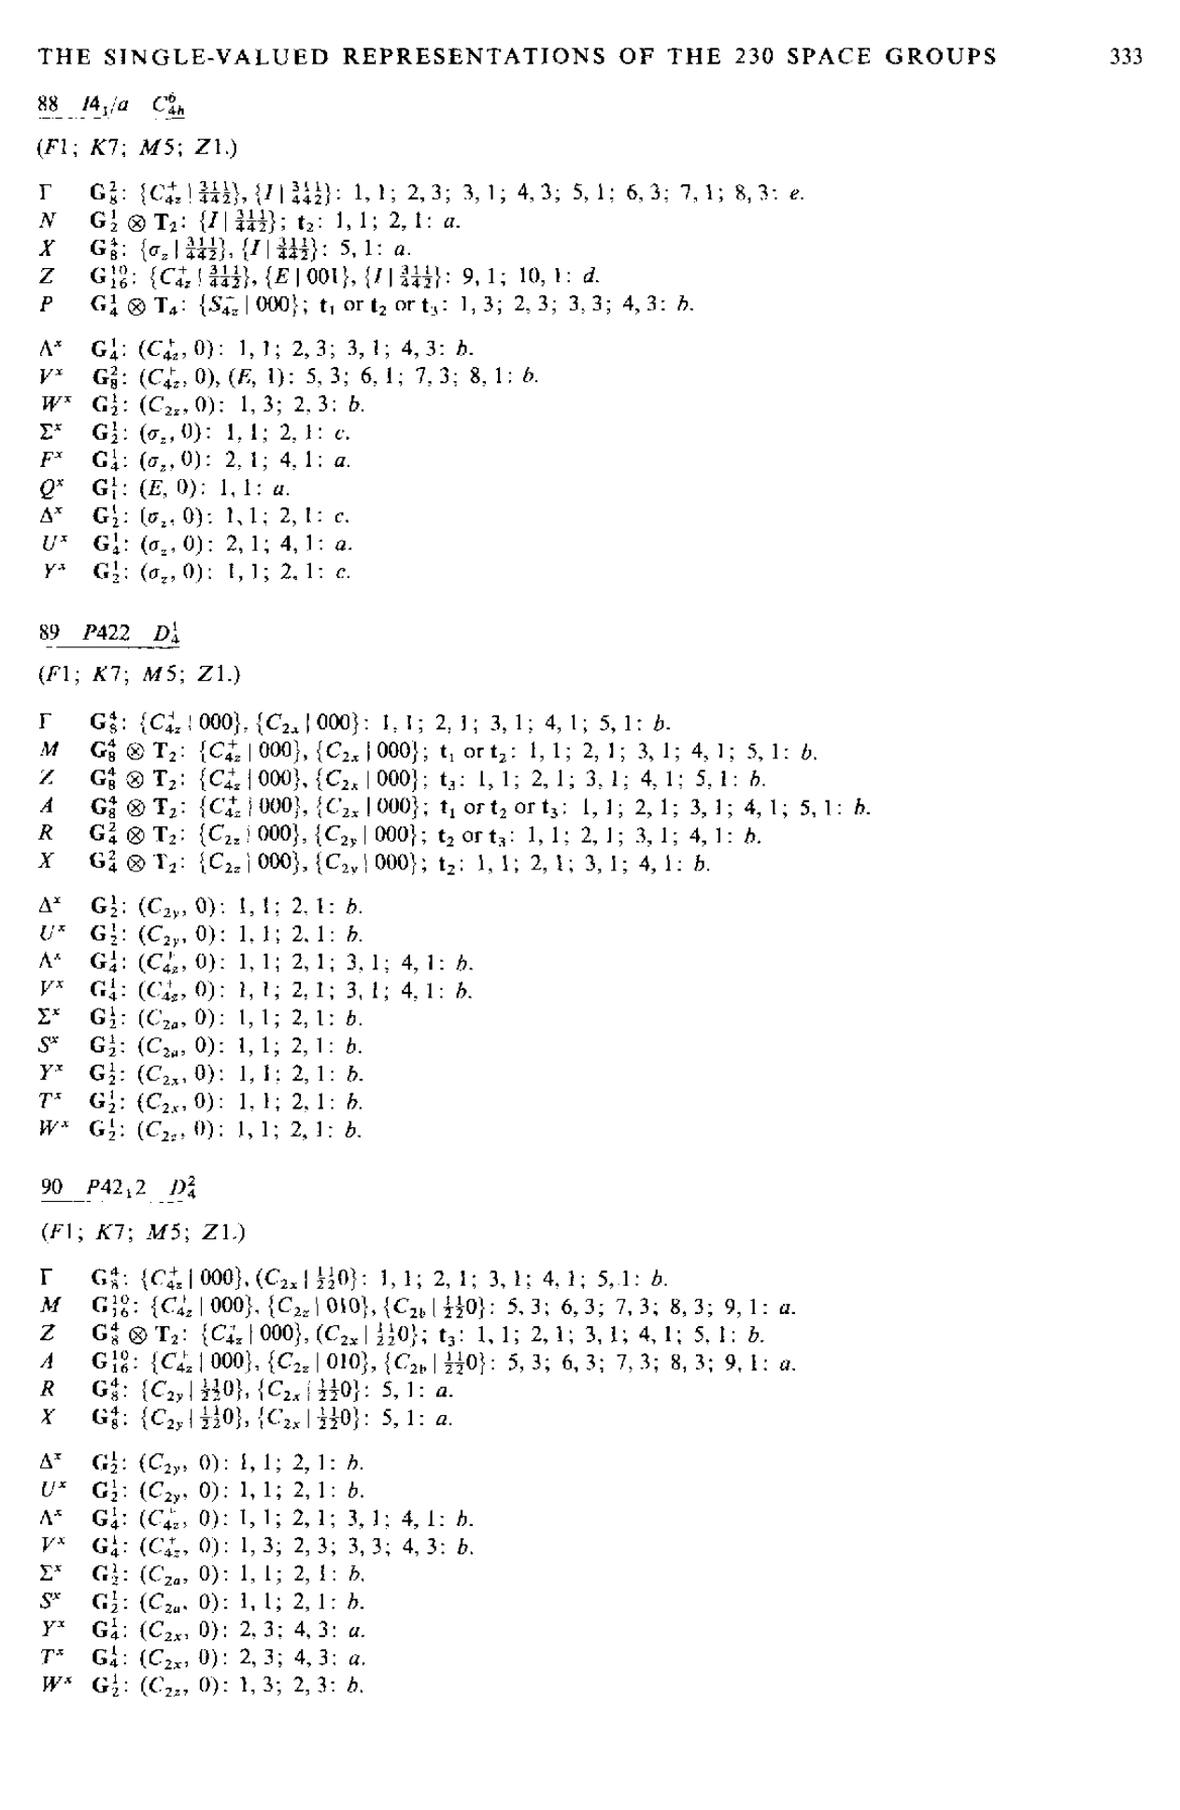
\includegraphics[width=0.86\textwidth]{c5_52_p346.jpg}
\caption*{原书第 333 页}
\end{figure}
\begin{figure}[H]
\centering
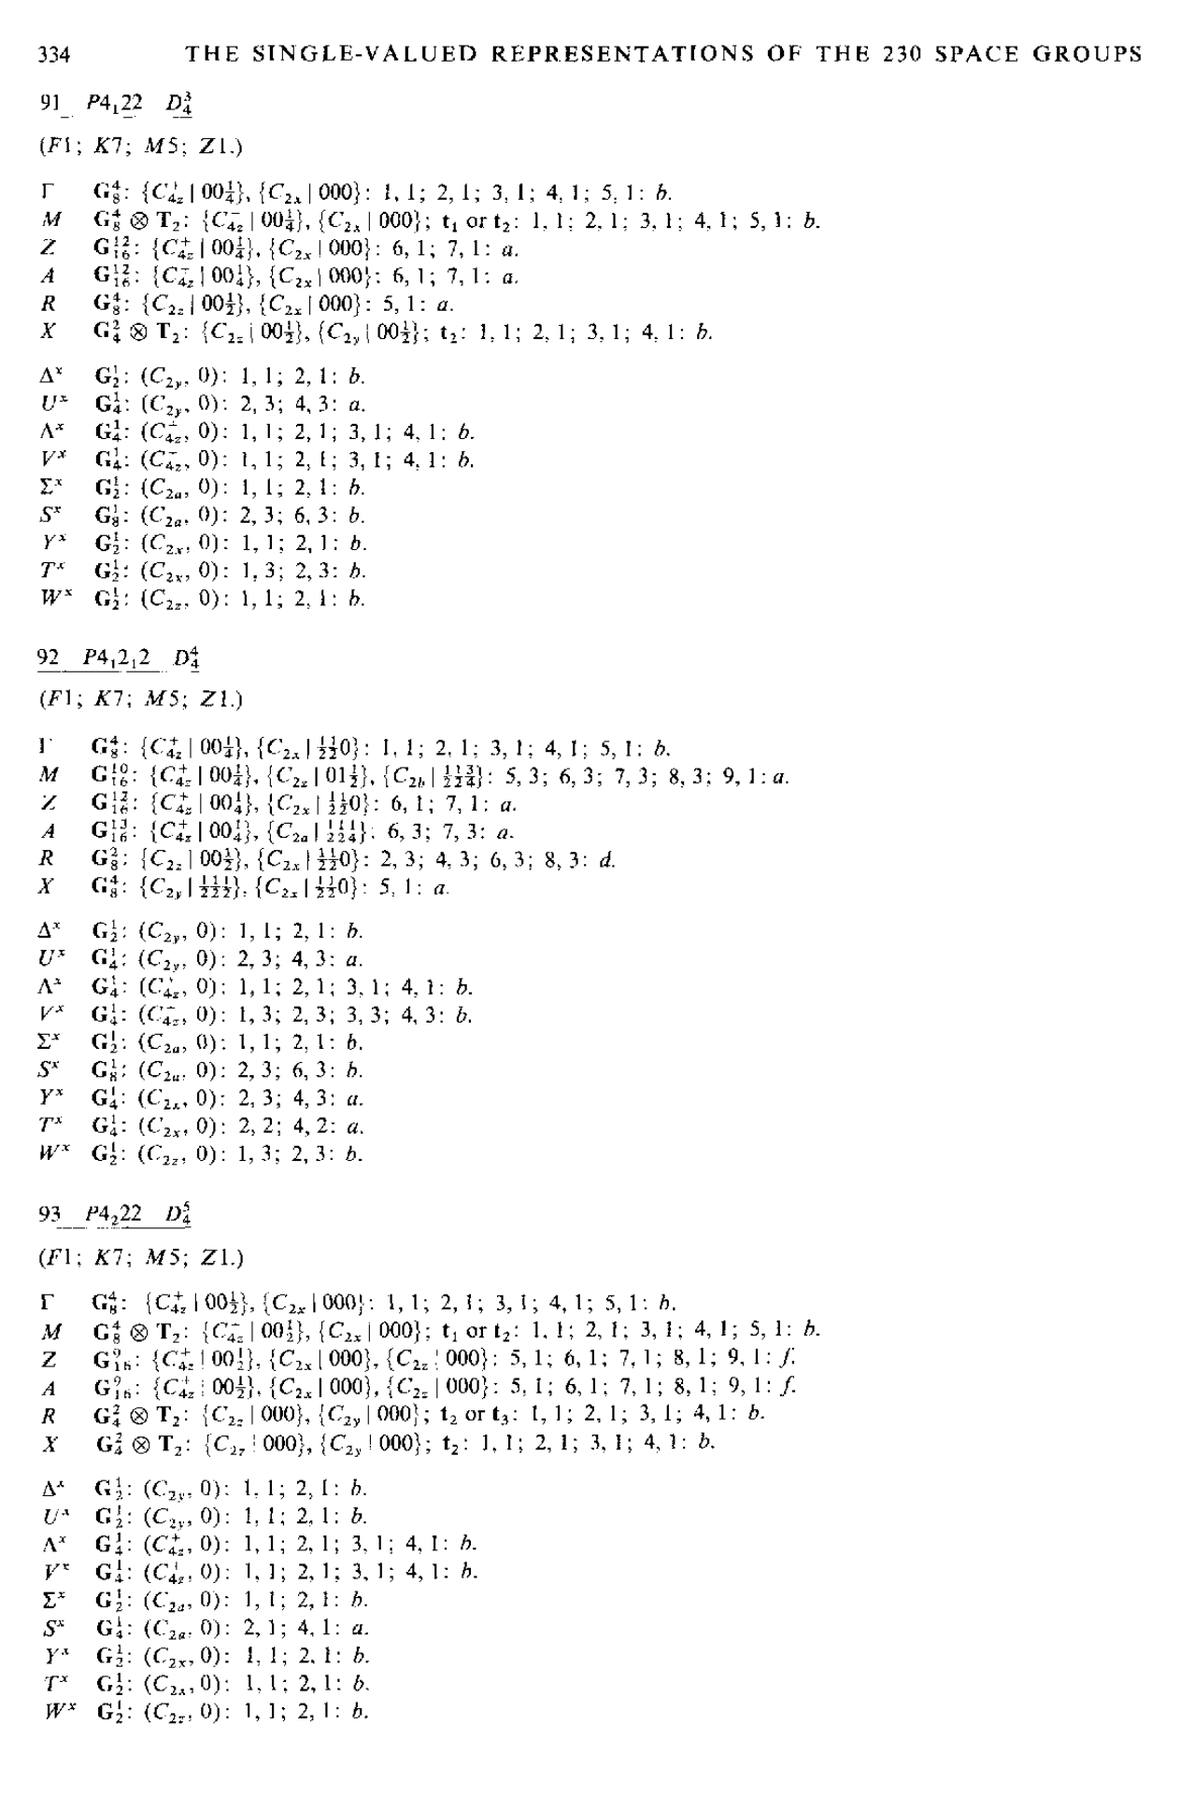
\includegraphics[width=0.86\textwidth]{c5_52_p347.jpg}
\caption*{原书第 334 页}
\end{figure}
\begin{figure}[H]
\centering
\includegraphics[width=0.86\textwidth]{c5_52_p348.jpg}
\caption*{原书第 335 页}
\end{figure}
\begin{figure}[H]
\centering
\includegraphics[width=0.86\textwidth]{c5_52_p349.jpg}
\caption*{原书第 336 页}
\end{figure}
\begin{figure}[H]
\centering
\includegraphics[width=0.86\textwidth]{c5_52_p350.jpg}
\caption*{原书第 337 页}
\end{figure}
\begin{figure}[H]
\centering
\includegraphics[width=0.86\textwidth]{c5_52_p351.jpg}
\caption*{原书第 338 页}
\end{figure}
\begin{figure}[H]
\centering
\includegraphics[width=0.86\textwidth]{c5_52_p352.jpg}
\caption*{原书第 339 页}
\end{figure}
\begin{figure}[H]
\centering
\includegraphics[width=0.86\textwidth]{c5_52_p353.jpg}
\caption*{原书第 340 页}
\end{figure}
\begin{figure}[H]
\centering
\includegraphics[width=0.86\textwidth]{c5_52_p354.jpg}
\caption*{原书第 341 页}
\end{figure}
\begin{figure}[H]
\centering
\includegraphics[width=0.86\textwidth]{c5_52_p355.jpg}
\caption*{原书第 342 页}
\end{figure}
\begin{figure}[H]
\centering
\includegraphics[width=0.86\textwidth]{c5_52_p356.jpg}
\caption*{原书第 343 页}
\end{figure}
\begin{figure}[H]
\centering
\includegraphics[width=0.86\textwidth]{c5_52_p357.jpg}
\caption*{原书第 344 页}
\end{figure}
\begin{figure}[H]
\centering
\includegraphics[width=0.86\textwidth]{c5_52_p358.jpg}
\caption*{原书第 345 页}
\end{figure}
\begin{figure}[H]
\centering
\includegraphics[width=0.86\textwidth]{c5_52_p359.jpg}
\caption*{原书第 346 页}
\end{figure}
\begin{figure}[H]
\centering
\includegraphics[width=0.86\textwidth]{c5_52_p360.jpg}
\caption*{原书第 347 页}
\end{figure}
\begin{figure}[H]
\centering
\includegraphics[width=0.86\textwidth]{c5_52_p361.jpg}
\caption*{原书第 348 页}
\end{figure}
\begin{figure}[H]
\centering
\includegraphics[width=0.86\textwidth]{c5_52_p362.jpg}
\caption*{原书第 349 页}
\end{figure}
\begin{figure}[H]
\centering
\includegraphics[width=0.86\textwidth]{c5_52_p363.jpg}
\caption*{原书第 350 页}
\end{figure}
\begin{figure}[H]
\centering
\includegraphics[width=0.86\textwidth]{c5_52_p364.jpg}
\caption*{原书第 351 页}
\end{figure}
\begin{figure}[H]
\centering
\includegraphics[width=0.86\textwidth]{c5_52_p365.jpg}
\caption*{原书第 352 页}
\end{figure}
\begin{figure}[H]
\centering
\includegraphics[width=0.86\textwidth]{c5_52_p366.jpg}
\caption*{原书第 353 页}
\end{figure}
\begin{figure}[H]
\centering
\includegraphics[width=0.86\textwidth]{c5_52_p367.jpg}
\caption*{原书第 354 页}
\end{figure}
\begin{figure}[H]
\centering
\includegraphics[width=0.86\textwidth]{c5_52_p368.jpg}
\caption*{原书第 355 页}
\end{figure}
\begin{figure}[H]
\centering
\includegraphics[width=0.86\textwidth]{c5_52_p369.jpg}
\caption*{原书第 356 页}
\end{figure}
\begin{figure}[H]
\centering
\includegraphics[width=0.86\textwidth]{c5_52_p370.jpg}
\caption*{原书第 357 页}
\end{figure}
\begin{figure}[H]
\centering
\includegraphics[width=0.86\textwidth]{c5_52_p371.jpg}
\caption*{原书第 358 页}
\end{figure}
\begin{figure}[H]
\centering
\includegraphics[width=0.86\textwidth]{c5_52_p372.jpg}
\caption*{原书第 359 页}
\end{figure}
\begin{figure}[H]
\centering
\includegraphics[width=0.86\textwidth]{c5_52_p373.jpg}
\caption*{原书第 360 页}
\end{figure}
\begin{figure}[H]
\centering
\includegraphics[width=0.86\textwidth]{c5_52_p374.jpg}
\caption*{原书第 361 页}
\end{figure}
\begin{figure}[H]
\centering
\includegraphics[width=0.86\textwidth]{c5_52_p375.jpg}
\caption*{原书第 362 页}
\end{figure}
\begin{figure}[H]
\centering
\includegraphics[width=0.86\textwidth]{c5_52_p376.jpg}
\caption*{原书第 363 页}
\end{figure}
\begin{figure}[H]
\centering
\includegraphics[width=0.86\textwidth]{c5_52_p377.jpg}
\caption*{原书第 364 页}
\end{figure}
\begin{figure}[H]
\centering
\includegraphics[width=0.86\textwidth]{c5_52_p378.jpg}
\caption*{原书第 365 页}
\end{figure}
\begin{figure}[H]
\centering
\includegraphics[width=0.86\textwidth]{c5_52_p379.jpg}
\caption*{原书第 366 页}
\end{figure}
\begin{figure}[H]
\centering
\includegraphics[width=0.86\textwidth]{c5_52_p380.jpg}
\caption*{原书第 367 页}
\end{figure}
\begin{figure}[H]
\centering
\includegraphics[width=0.86\textwidth]{c5_52_p381.jpg}
\caption*{原书第 368 页}
\end{figure}
\begin{figure}[H]
\centering
\includegraphics[width=0.86\textwidth]{c5_52_p382.jpg}
\caption*{原书第 369 页}
\end{figure}
\begin{figure}[H]
\centering
\includegraphics[width=0.86\textwidth]{c5_52_p383.jpg}
\caption*{原书第 370 页}
\end{figure}
\begin{figure}[H]
\centering
\includegraphics[width=0.86\textwidth]{c5_52_p384.jpg}
\caption*{原书第 371 页}
\end{figure}
\begin{figure}[H]
\centering
\includegraphics[width=0.86\textwidth]{c5_52_p385.jpg}
\caption*{原书第 372 页}
\end{figure}
\begin{figure}[H]
\centering
\includegraphics[width=0.86\textwidth]{c5_52_p386.jpg}
\caption*{原书第 373 页}
\end{figure}
\begin{figure}[H]
\centering
\includegraphics[width=0.86\textwidth]{c5_52_p387.jpg}
\caption*{原书第 374 页}
\end{figure}
\begin{figure}[H]
\centering
\includegraphics[width=0.86\textwidth]{c5_52_p388.jpg}
\caption*{原书第 375 页}
\end{figure}
\begin{figure}[H]
\centering
\includegraphics[width=0.86\textwidth]{c5_52_p389.jpg}
\caption*{原书第 376 页}
\end{figure}
\begin{figure}[H]
\centering
\includegraphics[width=0.86\textwidth]{c5_52_p390.jpg}
\caption*{原书第 377 页}
\end{figure}
\begin{figure}[H]
\centering
\includegraphics[width=0.86\textwidth]{c5_52_p391.jpg}
\caption*{原书第 378 页}
\end{figure}
\begin{figure}[H]
\centering
\includegraphics[width=0.86\textwidth]{c5_52_p392.jpg}
\caption*{原书第 379 页}
\end{figure}
\begin{figure}[H]
\centering
\includegraphics[width=0.86\textwidth]{c5_52_p393.jpg}
\caption*{原书第 380 页}
\end{figure}
\begin{figure}[H]
\centering
\includegraphics[width=0.86\textwidth]{c5_52_p394.jpg}
\caption*{原书第 381 页}
\end{figure}
\begin{figure}[H]
\centering
\includegraphics[width=0.86\textwidth]{c5_52_p395.jpg}
\caption*{原书第 382 页}
\end{figure}
\begin{figure}[H]
\centering
\includegraphics[width=0.86\textwidth]{c5_52_p396.jpg}
\caption*{原书第 383 页}
\end{figure}
\begin{figure}[H]
\centering
\includegraphics[width=0.86\textwidth]{c5_52_p397.jpg}
\caption*{原书第 384 页}
\end{figure}
\begin{figure}[H]
\centering
\includegraphics[width=0.86\textwidth]{c5_52_p398.jpg}
\caption*{原书第 385 页}
\end{figure}
\begin{figure}[H]
\centering
\includegraphics[width=0.86\textwidth]{c5_52_p399.jpg}
\caption*{原书第 386 页}
\end{figure}
\begin{figure}[H]
\centering
\includegraphics[width=0.86\textwidth]{c5_52_p400.jpg}
\caption*{原书第 387 页}
\end{figure}
\begin{figure}[H]
\centering
\includegraphics[width=0.86\textwidth]{c5_52_p401.jpg}
\caption*{原书第 388 页}
\end{figure}

% 5.3 空间群表示的标记
\section{空间群表示的标记}

在表 5.8 中我们给出了用于 ${}^{H}\mathbf{G}^{\mathbf{k}}$ 或 $\overline{\mathbf{G}}^{\mathbf{k}*}$ 的表示的标记。我们使用表 2.2 中点群表示所用的两种记号的推广，即 Mulliken (1933) 的记号（$A$、$B$、$E$、$T$ 等）以及 Koster, Dimmock, Wheeler, and Statz (1963) 的 $\Gamma_{1}, \Gamma_{2}, \Gamma_{3}$ 等记号。对许多空间群，${}^{H}\mathbf{G}^{\mathbf{k}}$ 或 $\overline{\mathbf{G}}^{\mathbf{k}*}$ 同构于 32 个点群之一，此时我们直接使用表 2.2 中该点群的标记。当 ${}^{H}\mathbf{G}^{\mathbf{k}}$ 或 $\overline{\mathbf{G}}^{\mathbf{k}*}$ 不同构于任何点群时，记号作如下推广（这里“实”指所有特征标都是实的，“复”指部分特征标是复的）：

\begin{center}
\begin{tabular}{ccl}
\toprule
表示 & 维数 & 标记\\
\midrule
实 & 1 & $A$ 或 $B$\\
复 & 1 & ${}^{1}E,\ {}^{2}E$（共轭对）\\
实 & 2 & $E$\\
复 & 2 & ${}^{1}F,\ {}^{2}F$（共轭对）\\
实 & 3 & $T$\\
复 & 3 & ${}^{1}H,\ {}^{2}H$（共轭对）\\
实 & 4 & $F$\\
复 & 4 & ${}^{1}J,\ {}^{2}J$（共轭对）\\
实 & 6 & $H$\\
\bottomrule
\end{tabular}
\end{center}

下标 1、2、3 等，下标 g 与 u，以及上标撇与双撇，用于区分同维数的表示，方式与点群标记中类似。若 ${}^{H}\mathbf{G}^{\mathbf{k}}$ 是 $(\{E \mid \mathbf{0}\} \oplus \{I \mid \mathbf{0}\})$ 与某个群 $\mathbf{G}$ 的直积，则用 $R_{g}$ 与 $R_{u}$ 表示由 $\mathbf{G}$ 的表示 $R$ 导出的两个表示：在 $R_{g}$ 中 $\chi(\{I \mid \mathbf{0}\})$ 为 $+\chi(\{E \mid \mathbf{0}\})$，在 $R_{u}$ 中 $\chi(\{I \mid \mathbf{0}\})$ 为 $-\chi(\{E \mid \mathbf{0}\})$。撇与双撇用于区分仅仅在一个重要反射面的特征标符号上不同的两个表示 $R'_{i}$ 与 $R''_{i}$。在 $\Gamma$ 记法中，表示标记为 $\Gamma_{1}, \Gamma_{2}, \Gamma_{3}$ 等；上标 $+$ 与 $-$ 通常用于直积群的表示，用法与上面的 g 和 u 类似（Miller and Love (1967) 除外）。在对称点上（$\Gamma$ 以外的点）或对称线上，$\Gamma$ 换成表示该点或线的字母。例如，在 $P4_{3}32\ (O^{6})$ 的 $M$ 点，与抽象群 $\mathbf{G}^{10}_{16}$ 的表示 $R_{5}, R_{6}, R_{7}, R_{8}, R_{9}$ 认同的空间群表示，按表 5.8 中 $\mathbf{G}^{10}_{16}$ 下的条目“a”，或者标记为 ${}^{2}E_{1}, {}^{1}E_{1}, {}^{1}E_{2}, {}^{2}E_{2}$ 与 $E$，或者标记为 $M_{1}, M_{2}, M_{3}, M_{4}$ 与 $M_{5}$，其中 $\Gamma_{i}$ 已换成 $M_{i}$。

在这两种记法中都不可能完全合乎逻辑地定义一套标记。也难于综合研究过个别空间群或少量空间群的各位作者所用的所有标记。

\begin{figure}[H]
\centering
\includegraphics[width=0.86\textwidth]{c5_t58_p01.jpg}
\caption*{\textbf{表 5.8}\ 空间群表示的标记（原书第 390 页起扫描；第 1 页，共 7 页）。}
\end{figure}
\begin{figure}[H]
\centering
\includegraphics[width=0.86\textwidth]{c5_t58_p02.jpg}
\caption*{\textbf{表 5.8}（第 2 页）。}
\end{figure}
\begin{figure}[H]
\centering
\includegraphics[width=0.86\textwidth]{c5_t58_p03.jpg}
\caption*{\textbf{表 5.8}（第 3 页）。}
\end{figure}
\begin{figure}[H]
\centering
\includegraphics[width=0.86\textwidth]{c5_t58_p04.jpg}
\caption*{\textbf{表 5.8}（第 4 页）。}
\end{figure}
\begin{figure}[H]
\centering
\includegraphics[width=0.86\textwidth]{c5_t58_p05.jpg}
\caption*{\textbf{表 5.8}（第 5 页）。}
\end{figure}
\begin{figure}[H]
\centering
\includegraphics[width=0.86\textwidth]{c5_t58_p06.jpg}
\caption*{\textbf{表 5.8}（第 6 页）。}
\end{figure}
\begin{figure}[H]
\centering
\includegraphics[width=0.86\textwidth]{c5_t58_p07.jpg}
\caption*{\textbf{表 5.8}（第 7 页）。}
\end{figure}

% 5.4 空间群表示表的使用示例
\section{空间群表示表的使用示例}

立方密堆积与金刚石结构（$Fm3m\ (O^{5}_{h})$ 与 $Fd3m\ (O^{7}_{h})$）的空间群表示已在 3.8 节作为推导空间群表示的理论之例导出。现在我们给出一个例子，说明如何使用表 5.7 与 5.8 为 230 个空间群中的任何一个检索类似的信息。我们留给读者一个附加练习：验证 3.8 节讨论过的 $Fm3m\ (O^{5}_{h})$ 与 $Fd3m\ (O^{7}_{h})$ 的空间群表示如何能从表 5.7 与 5.8 得到。

\begin{figure}[H]
\centering
\includegraphics[width=0.62\textwidth]{fig5_2_mu.jpg}
\caption*{\textbf{图 5.2}\ $\Gamma^{f}_{c}$ 的布里渊区。$\Gamma=(000)$；$X=(\frac{1}{2}0\frac{1}{2})$；$L=(\frac{1}{2}\frac{1}{2}\frac{1}{2})$；$W=(\frac{1}{2}\frac{1}{4}\frac{3}{4})$。$X$ 与 $U$ 虽常被称为对称点，但按定义 3.3.1 它们并不算对称点，因为它们并不比相邻的线 $\Delta$ 与 $S$ 具有更多对称性。}
\end{figure}

空间群 $F\bar{4}3c\ (T^{5}_{d})$ 在表 5.7 的注中已多次用作示例，这里用它进一步演示该表的用法。$F\bar{4}3c\ (T^{5}_{d})$ 是关联于点群 $\bar{4}3m\ (T_{d})$、建立在面心立方布拉维格子 $\Gamma^{f}_{c}$ 上的立方空间群，由表 3.1 其基本矢量为
\begin{equation*}
\left\{
\begin{array}{l}
\mathbf{t}_{1} = \frac{1}{2}(0, a, a),\\
\mathbf{t}_{2} = \frac{1}{2}(a, 0, a),\\
\mathbf{t}_{3} = \frac{1}{2}(a, a, 0),
\end{array}
\right.
\tag{5.4.1}
\end{equation*}
而
\begin{equation*}
\left\{
\begin{array}{l}
\mathbf{g}_{1} = (2\pi/a)(-1, 1, 1),\\
\mathbf{g}_{2} = (2\pi/a)(1, -1, 1),\\
\mathbf{g}_{3} = (2\pi/a)(1, 1, -1).
\end{array}
\right.
\tag{5.4.2}
\end{equation*}
因此倒格子是体心立方格子（见表 3.3），其布里渊区示于图 3.14 并复制为图 5.2。由表 3.6（$\Gamma^{f}_{c}$ 名下）或表 5.7，该布里渊区中特殊的对称点是 $\Gamma$、$X$、$L$ 与 $W$；一些作者把 $K$ 也当作对称点，但如图 3.14 的题注所指出的，它不符合我们关于对称点的定义（见定义 3.3.1）。类似地，对称线为 $\Delta$、$\Lambda$、$\Sigma$、$S$、$Z$ 与 $Q$。对称面不予考虑。各对称点和对称线的 $\mathbf{k}$ 矢量在表 3.6 中以 $\mathbf{g}_{1}, \mathbf{g}_{2}, \mathbf{g}_{3}$ 的单位给出：
\begin{center}
\begin{tabular}{lc}
点或线 & $\mathbf{k}$\\
\midrule
$\Gamma$ & $(000)$\\
$X$ & $(\frac{1}{2}0\frac{1}{2})$\\
$L$ & $(\frac{1}{2}\frac{1}{2}\frac{1}{2})$\\
$W$ & $(\frac{1}{2}\frac{1}{4}\frac{3}{4})$\\
$\Delta$ & $(\alpha 0\alpha)$\\
$\Lambda$ & $(\alpha\alpha\alpha)$\\
$\Sigma$ & $(\alpha, \alpha, 2\alpha)$\\
$S$ & $(\frac{1}{2}+\alpha, 2\alpha, \frac{1}{2}+\alpha)$\\
$Z$ & $(\frac{1}{2}, \alpha, \frac{1}{2}+\alpha)$\\
$Q$ & $(\frac{1}{2}, \frac{1}{2}-\alpha, \frac{1}{2}+\alpha)$
\end{tabular}
\end{center}

我们逐一考虑各个对称点。

\noindent\textbf{$\Gamma$：$\mathbf{k} = (000)$。}

${}^{H}\mathbf{G}^{\Gamma}$ 是 $\mathbf{G}^{7}_{24}$，它同构于点群 $\bar{4}3m\ (T_{d})$，其生成元为
\begin{equation*}
P = \{C^{-}_{31} \mid 000\}, \qquad Q = \{C_{2z} \mid 000\},
\end{equation*}
\begin{equation*}
R = \{C_{2x} \mid 000\}, \qquad S = \{\sigma_{da} \mid {\textstyle\frac{1}{2}}{\textstyle\frac{1}{2}}{\textstyle\frac{1}{2}}\}.
\end{equation*}
五个类（见表 5.1）为
\begin{center}
\begin{tabular}{l}
$C_{1} = \{E \mid 000\}$；\\
$C_{2} = \{C_{2x} \mid 000\}, \{C_{2y} \mid 000\}, \{C_{2z} \mid 000\}$；\\
$C_{3} = \{S^{-}_{4x} \mid {\frac{1}{4}}{\frac{3}{4}}{\frac{1}{4}}\}$ 及其余五个 $S^{\pm}_{4m}$ 项；\\
$C_{4} = \{\sigma_{da} \mid {\frac{1}{4}}{\frac{3}{4}}{\frac{1}{4}}\}$ 及其余五个 $\sigma_{dm}$ 项；\\
$C_{5} = \{C^{-}_{31} \mid 000\}, \dots, \{C^{+}_{34} \mid 000\}$（八个 $C^{\pm}_{3j}$）。
\end{tabular}
\end{center}
要辨认 $\mathbf{G}^{7}_{24}$ 的哪个元素对应于哪个空间群元素相当费事，必须直接相乘。见表 5.7 的注 (iv)，那里证明了 $\mathbf{G}^{7}_{24}$ 的 $P^{2}RS$ 对应于 $\{S^{-}_{4y} \mid {\frac{1}{2}}\,{-\frac{3}{4}}\,{\frac{1}{4}}\}$，或平移至 $\mathbf{F}$ 后为 $\{S^{-}_{4y} \mid {\frac{1}{2}}{\frac{1}{4}}{\frac{1}{4}}\}$。如果要求的是简并表示的实际矩阵代表而不仅是特征标，这种认定当然是必须做的。于是 ${}^{H}\mathbf{G}^{\Gamma}$ 的特征标表可由表 5.1 的 $\mathbf{G}^{7}_{24}$ 条目查得，只是表示不标记为 $R_{1}, \dots, R_{5}$，而按表 5.8 中 $\mathbf{G}^{7}_{24}$ 下的条目“a”标记：
\begin{center}
\begin{tabular}{lccccc}
 & $R_{1}$ & $R_{2}$ & $R_{3}$ & $R_{4}$ & $R_{5}$\\
a & $A_{1}$ $\Gamma_{1}$ & $A_{2}$ $\Gamma_{2}$ & $E$ $\Gamma_{3}$ & $T_{1}$ $\Gamma_{4}$ & $T_{2}$ $\Gamma_{5}$
\end{tabular}
\end{center}
由表 5.7 可见这些空间群表示全为第一种，于是 ${}^{H}\mathbf{G}^{\Gamma}$ 的特征标表为（右列给出相应空间群表示的实性）：
\begin{center}
\begin{tabular}{lcccccc}
 & $C_{1}$ & $C_{2}$ & $C_{3}$ & $C_{4}$ & $C_{5}$ & \\
$\Gamma_{1}\ A_{1}$ & 1 & 1 & 1 & 1 & 1 & 1\\
$\Gamma_{2}\ A_{2}$ & 1 & 1 & $-1$ & 1 & 1 & 1\\
$\Gamma_{3}\ E$ & 2 & 2 & 0 & 0 & $-1$ & 1\\
$\Gamma_{4}\ T_{1}$ & 3 & $-1$ & 1 & $-1$ & 0 & 1\\
$\Gamma_{5}\ T_{2}$ & 3 & $-1$ & $-1$ & 1 & 0 & 1
\end{tabular}
\end{center}
若计及时间反演对称，也没有额外简并。

\noindent\textbf{$X$：$\mathbf{k} = (\frac{1}{2}0\frac{1}{2})$。}

${}^{H}\mathbf{G}^{X}$ 是 $\mathbf{G}^{4}_{8}$ 与 $\mathbf{T}_{2}$ 的直积，$\mathbf{G}^{4}_{8}$ 的生成元为
\begin{equation*}
P = \left\{S^{+}_{4y} \mid {\textstyle\frac{1}{2}}{\textstyle\frac{1}{2}}{\textstyle\frac{1}{2}}\right\}, \qquad Q = \{C_{2x} \mid 000\},
\end{equation*}
$\mathbf{T}_{2}$ 的元素为 $\{E \mid \mathbf{0}\}$ 与 $\{E \mid \mathbf{t}_{s}\}$（$s = 1$ 或 3）。于是 $\mathbf{G}^{4}_{8}$ 的元素为
\begin{center}
\begin{tabular}{llll}
$E$ & $\{E \mid 000\}$ & $Q$ & $\{C_{2x} \mid 000\}$\\
$P$ & $\{S^{+}_{4y} \mid {\frac{1}{2}}{\frac{1}{2}}{\frac{1}{2}}\}$ & $PQ$ & $\{C_{2c} \mid {\frac{1}{2}}{\frac{1}{2}}{\frac{1}{2}}\}$\\
$P^{2}$ & $\{C_{2y} \mid 000\}$ & $P^{2}Q$ & $\{C_{2z} \mid 000\}$\\
$P^{3}$ & $\{S^{-}_{4y} \mid {\frac{1}{2}}{\frac{1}{2}}{\frac{1}{2}}\}$ & $P^{3}Q$ & $\{C_{2e} \mid {\frac{1}{2}}{\frac{1}{2}}{\frac{1}{2}}\}$
\end{tabular}
\end{center}
由表 5.1 它们可归入类 $C_{1}, C_{2}, \dots, C_{5}$。五个表示按表 5.8 标记为 $A_{1}, A_{2}, B_{1}, B_{2}$ 与 $E$（即 $X_{1}, X_{2}, X_{3}, X_{4}$ 与 $X_{5}$）。于是 ${}^{H}\mathbf{G}^{X}$ 的特征标表为（右列给出实性）：
\begin{center}
\begin{tabular}{lccccccc}
 & & $\{E \mid 000\}$ & $\{C_{2y} \mid 000\}$ & $\begin{array}{c}\{S^{+}_{4y} \mid {\frac{1}{4}}{\frac{3}{4}}{\frac{1}{4}}\}\\ \{S^{-}_{4y} \mid {\frac{1}{4}}{\frac{3}{4}}{\frac{1}{4}}\}\end{array}$ & $\begin{array}{c}\{C_{2x} \mid 000\}\\ \{C_{2z} \mid 000\}\end{array}$ & $\begin{array}{c}\{C_{2c} \mid {\frac{1}{4}}{\frac{3}{4}}{\frac{1}{4}}\}\\ \{C_{2e} \mid {\frac{1}{4}}{\frac{3}{4}}{\frac{1}{4}}\}\end{array}$ & \\
$X_{1}$ & $A_{1}$ & 1 & 1 & 1 & 1 & 1 & 1\\
$X_{2}$ & $A_{2}$ & 1 & 1 & 1 & $-1$ & $-1$ & 1\\
$X_{3}$ & $B_{1}$ & 1 & 1 & $-1$ & 1 & $-1$ & 1\\
$X_{4}$ & $B_{2}$ & 1 & 1 & $-1$ & $-1$ & 1 & 1\\
$X_{5}$ & $E$ & 2 & $-2$ & 0 & 0 & 0 & 1
\end{tabular}
\end{center}
若计及时间反演对称，将没有额外简并。若需要表示 $E\ (X_{5})$ 的矩阵，它们也可由表 5.1 中 $\mathbf{G}^{4}_{8}$ 的 $R_{5}$ 得到。

\noindent\textbf{$L$：$\mathbf{k} = (\frac{1}{2}\frac{1}{2}\frac{1}{2})$。}

${}^{H}\mathbf{G}^{L}$ 是 $\mathbf{G}^{4}_{12}$，其生成元为
\begin{equation*}
P = \{C^{-}_{31} \mid 001\}, \qquad Q = \{\sigma_{db} \mid {\textstyle\frac{1}{2}}{\textstyle\frac{1}{2}}{\textstyle\frac{1}{2}}\},
\end{equation*}
而 ${}^{H}\mathbf{G}^{L}$ 的十二个成员为
\begin{center}
\begin{tabular}{llll}
$E$ & $\{E \mid 000\}$ & $Q$ & $\{\sigma_{db} \mid {\frac{1}{2}}{\frac{1}{2}}{\frac{1}{2}}\}$\\
$P$ & $\{C^{-}_{31} \mid 001\}$ & $PQ$ & $\{\sigma_{df} \mid {\frac{1}{2}}{\frac{1}{2}}{-\frac{1}{2}}\}$\\
$P^{2}$ & $\{C^{+}_{31} \mid 000\}$ & $P^{2}Q$ & $\{\sigma_{de} \mid {\frac{1}{2}}{\frac{1}{2}}{\frac{1}{2}}\}$\\
$P^{3}$ & $\{E \mid 001\}$ & $P^{3}Q$ & $\{\sigma_{db} \mid {\frac{1}{2}}{\frac{1}{2}}{-\frac{1}{2}}\}$\\
$P^{4}$ & $\{C^{-}_{31} \mid 000\}$ & $P^{4}Q$ & $\{\sigma_{df} \mid {\frac{1}{2}}{\frac{1}{2}}{\frac{1}{2}}\}$\\
$P^{5}$ & $\{C^{+}_{31} \mid 001\}$ & $P^{5}Q$ & $\{\sigma_{de} \mid {\frac{1}{2}}{\frac{1}{2}}{-\frac{1}{2}}\}$
\end{tabular}
\end{center}
它们可归入 $\mathbf{G}^{4}_{12}$ 的类，从而构造出 ${}^{H}\mathbf{G}^{L}$ 的特征标表：
\begin{center}
\begin{tabular}{lccccccc}
 & $\{E \mid 000\}$ & $\{E \mid 001\}$ & $\begin{array}{c}\{C^{-}_{31} \mid 001\}\\ \{C^{+}_{31} \mid 001\}\end{array}$ & $\begin{array}{c}\{C^{+}_{31} \mid 000\}\\ \{C^{-}_{31} \mid 000\}\end{array}$ & $\begin{array}{c}\{\sigma_{db} \mid {\frac{1}{2}}{\frac{1}{2}}{\frac{1}{2}}\}\\ \{\sigma_{de}\},\{\sigma_{df}\}\end{array}$ & $\begin{array}{c}\{\sigma_{db} \mid {\frac{1}{2}}{\frac{1}{2}}{-\frac{1}{2}}\}\\ \{\sigma_{de}\},\{\sigma_{df}\}\end{array}$ & \\
$L_{1}$\ \ ${}^{2}E$ & 1 & $-1$ & $-1$ & 1 & $i$ & $-i$ & 3\\
$L_{2}$\ \ ${}^{1}E$ & 1 & $-1$ & $-1$ & 1 & $-i$ & $i$ & 3\\
$L_{3}$\ \ $E$ & 2 & $-2$ & 1 & $-1$ & 0 & 0 & 2
\end{tabular}
\end{center}
$E\ (L_{3})$ 的矩阵可由表 5.1 中 $\mathbf{G}^{4}_{12}$ 的 $R_{6}$ 得到。最右列的实性表明：若计及时间反演对称，${}^{1}E$ 与 ${}^{2}E$（$L_{2}$ 与 $L_{1}$）之间出现额外简并，属于表示 $E\ (L_{3})$ 的两组不同基函数之间也出现额外简并。

\noindent\textbf{$W$：$\mathbf{k} = (\frac{1}{2}\frac{1}{4}\frac{3}{4})$。}

${}^{H}\mathbf{G}^{W}$ 是 $\mathbf{G}^{1}_{4}$ 与 $\mathbf{T}_{4}$ 的直积，其中 $\mathbf{T}_{4}$ 由 $\{E \mid \mathbf{0}\}$、$\{E \mid \mathbf{t}_{2}\}$、$\{E \mid 2\mathbf{t}_{2}\}$、$\{E \mid 3\mathbf{t}_{2}\}$ 组成，而 $\mathbf{G}^{1}_{4}$ 的生成元为 $P = \{S^{+}_{4x} \mid {\frac{1}{4}}{\frac{1}{2}}{\frac{1}{4}}\}$。$\mathbf{G}^{1}_{4}$ 的每个元素自成一类，于是 ${}^{H}\mathbf{G}^{W}$ 的特征标表为
\begin{center}
\begin{tabular}{lccccc}
 & $\{E \mid 000\}$ & $\{S^{+}_{4x} \mid {\frac{1}{4}}{\frac{1}{2}}{\frac{1}{4}}\}$ & $\{C_{2x} \mid 000\}$ & $\{S^{-}_{4x} \mid {\frac{1}{4}}{\frac{1}{2}}{\frac{1}{4}}\}$ & \\
$W_{1}\ A$ & 1 & 1 & 1 & 1 & 3\\
$W_{2}\ {}^{2}E$ & 1 & $i$ & $-1$ & $-i$ & 3\\
$W_{3}\ B$ & 1 & $-1$ & 1 & $-1$ & 3\\
$W_{4}\ {}^{1}E$ & 1 & $-i$ & $-1$ & $i$ & 3
\end{tabular}
\end{center}
最右列的实性表明：若计及时间反演对称，属于不同表示的本征函数对之间出现额外简并；具体地说，$A\ (W_{1})$ 与 $B\ (W_{3})$ 变为简并，${}^{1}E\ (W_{4})$ 与 ${}^{2}E\ (W_{2})$ 变为简并（见 7.6 与 7.7 节）。

至此本空间群的对称点考虑完毕，接下来考虑对称线，这要用到 3.7 节描述的射影表示理论。对每条对称线，我们先辨认中央延拓群 $\overline{\mathbf{G}}^{\mathbf{k}*}$，再由它得到小群 $\mathbf{G}^{\mathbf{k}}$ 的表示。$\overline{\mathbf{G}}^{\mathbf{k}*}$ 的元素形如 $(H_{j}, \alpha)$，其中 $H_{j}$ 是某个空间群元素的点群操作部分，$\alpha$ 是式 (3.7.27) 定义的循环群 $\mathbf{Z}_{g}$ 的一个小整数。群 $\overline{\mathbf{G}}^{\mathbf{k}*}$ 在表 5.7 中指明，其生成元 $P, Q, \dots$ 依次以 $(H_{j}, \alpha)$ 的形式给出。于是 $\overline{\mathbf{G}}^{\mathbf{k}*}$ 的特征标表与矩阵代表可由表 5.1 辨认，而 $\mathbf{G}^{\mathbf{k}}$ 的表示对每个元素 $\{R \mid \mathbf{v}\}$ 由 $(R, 0)$ 的矩阵代表乘以因子 $\exp(-\mathrm{i}\mathbf{k} \cdot \mathbf{v})$ 得到（见式 (3.8.8) 与 (3.8.9)）。表示的标记可查表 5.7 中相应线条目所指出的表 5.8 的部分。注意，当 $\overline{\mathbf{G}}^{\mathbf{k}*}$ 的表示与 $(E, 1)$ 生成的循环群 $\mathbf{Z}_{g}$ 的允许表示不相容时，它们被略去（见式 (3.7.33)）。还应注意，一般 $\mathbf{G}^{\mathbf{k}}$ 的类结构可能与 $\overline{\mathbf{G}}^{\mathbf{k}*}$ 的不同，而且由于 $\mathbf{G}^{\mathbf{k}}$ 无限，确定 $\mathbf{G}^{\mathbf{k}}$ 的类结构可能相当复杂。相应空间群表示的实性（从而计及时间反演对称后的额外简并）也可由表 5.7 得到。下面以所选空间群 $F\bar{4}3c\ (T^{5}_{d})$ 的对称线为例说明。

以 $\Delta$ 线为例：中央延拓群 $\overline{\mathbf{G}}^{\Delta*}$ 是群 $\mathbf{G}^{2}_{4}$，其生成元为
\begin{equation*}
P = (C_{2y}, 0), \qquad Q = (\sigma_{dc}, 0).
\end{equation*}
由于 $\mathbf{G}^{2}_{4}$ 的阶为 4（与含 $E, C_{2y}, \sigma_{dc}, \sigma_{de}$ 的点群同阶），显然 $g$ 必为 1，于是 $\overline{\mathbf{G}}^{\Delta*}$ 的四个元素按类为：$C_{1}$：$(E, 0)$；$C_{2}$：$(C_{2y}, 0)$；$C_{3}$：$(\sigma_{dc}, 0)$；$C_{4}$：$(\sigma_{de}, 0)$。由表 5.1 得 $\overline{\mathbf{G}}^{\Delta*}$ 的特征标表，并用表 5.8 给出表示的标记。$\mathbf{G}^{\Delta}$ 的小表示即上表每项乘以因子 $\exp(-\mathrm{i}\mathbf{k} \cdot \mathbf{v})$：
\begin{center}
\begin{tabular}{lccccc}
 & $\{E \mid 000\}$ & $\{C_{2y} \mid 000\}$ & $\{\sigma_{dc} \mid {\frac{1}{2}}{\frac{1}{2}}{\frac{1}{2}}\}$ & $\{\sigma_{de} \mid {\frac{1}{2}}{\frac{1}{2}}{\frac{1}{2}}\}$ & \\
$\Delta_{1}\ A_{1}$ & 1 & 1 & $\Lambda$ & $\Lambda$ & 1\\
$\Delta_{3}\ A_{2}$ & 1 & 1 & $-\Lambda$ & $-\Lambda$ & 1\\
$\Delta_{2}\ B_{1}$ & 1 & $-1$ & $\Lambda$ & $-\Lambda$ & 3\\
$\Delta_{4}\ B_{2}$ & 1 & $-1$ & $-\Lambda$ & $\Lambda$ & 3
\end{tabular}
\end{center}
其中 $\Lambda = \exp(-2\pi\mathrm{i}\alpha)$。计及时间反演对称后，$A_{1}\ (\Delta_{1})$ 与 $A_{2}\ (\Delta_{3})$ 没有额外简并，但 $B_{1}\ (\Delta_{2})$ 与 $B_{2}\ (\Delta_{4})$ 变为简并。

\noindent（中译者注：原书随后对 $\Lambda, \Sigma, S, Z, Q$ 各线按同一 recipe 逐一处理（原书第 402--405 页），即辨认中央延拓群 $\overline{\mathbf{G}}^{\mathbf{k}*}$（表 5.1 + 表 5.7）并乘以相因子 $\exp(-\mathrm{i}\mathbf{k} \cdot \mathbf{v})$，此处从略；结果可直接由表 5.7 读出。）

空间群表示的用途现已扩展到晶体 lattice 正则振动的标记，即声子色散曲线的标记（Johnson and Loudon 1964；综述见 Maradudin and Vosko (1968) 与 Warren (1968)），也扩展到磁性晶体中自旋波色散关系的标记（Dimmock and Wheeler 1962\textit{b}, Joshua and Cracknell 1969, Loudon 1968）。最初声子色散曲线的实验测量只限于元素立方材料的高对称方向；在这种情形正则模可以相当充分地分类并标记为纯纵声学（LA）、横声学（TA）、纵光学（LO）或横光学（TO）。然而这个简单方案不适用于低对称方向或更复杂的晶体，所以现在正则模通常用空间群表示来标记。正如分子的正则振动可以群论地研究并归属于该分子点群的各表示（例如见 Cotton (1963), Cracknell (1968\textit{b}), Leech and Newman (1969)），具有给定波矢 $\mathbf{k}$ 的晶体正则振动也可以归属于该晶体空间群 $\mathbf{G}$ 的各表示。做法是研究晶胞中原子的一般位移 $\mathbf{x}_{i}$ 在空间群 $\mathbf{G}$ 操作下的变换性质。这样得到以 $\mathbf{x}_{i}$ 为基的表示 $\Gamma$，它一般可约。$\mathbf{k}$ 处正则模所属的 $\mathbf{G}^{\mathbf{k}}$ 的小表示于是可由 $\Gamma$ 的约化得到，小表示的标记随后用来标记布里渊区中 $\mathbf{k}$ 矢量的声子色散关系。另一种做法是：通过研究产生与湮灭算符 $a^{\dagger}_{\mathbf{k}}$ 与 $a_{\mathbf{k}}$ 在 $\mathbf{G}$ 操作下的变换性质、并把它们归属到 $\mathbf{G}^{\mathbf{k}}$ 的相应小表示，来确定波矢为 $\mathbf{k}$ 的正则模的对称性质；$a^{\dagger}_{\mathbf{k}}$ 与 $a_{\mathbf{k}}$ 是产生与湮灭波矢为 $\mathbf{k}$ 的声子的算符，其形式例如见 Kittel (1963)。磁性晶体自旋波色散关系按空间群表示的标记，可以通过研究类似于 $a^{\dagger}_{\mathbf{k}}$、$a_{\mathbf{k}}$ 的、产生与湮灭磁振子的相应算符在 $\mathbf{G}$ 操作下的变换性质来确定（Loudon 1968）。对某些特定空间群对称适配函数的确定，可见 Cornwell (1969) 一书的附录 3。在相对论性能带结构计算中必须使用双值空间群表示，这将在第六章讨论。

% 5.5 表示域与基本域
\section{表示域与基本域}

在表 5.7（以及 Miller and Love (1967) 的表）中，空间群表示只对 230 个空间群中每一个的布里渊区仅仅一个基本域（见定义 3.3.3）内的特殊对称点与对称线列出。回顾基本域 $\Omega$ 具有性质 $(\sum_{R}R\Omega)$ 等于整个布里渊区，其中算符 $R$ 取遍相应晶系全对称点群 $\mathbf{P}$ 的元素。例如对立方晶体，基本域只是布里渊区的四十八分之一。由于在讨论物理问题时可能会用到它们，为了完整性，必须考虑：给定仅仅一个基本域内的小表示之后，如何确定与布里渊区中其他点或对称线相联系的小表示。回顾表示域 $\Phi$（见定义 3.7.1）具有性质 $(\sum_{S}S\Phi)$ 等于整个布里渊区，其中算符 $S$ 取遍所考虑空间群 $\mathbf{G}$ 的同形点群 $\mathbf{F}$ 的元素。例如对空间群 $Pa3\ (T^{5}_{h})$，同形点群是 $m3\ (T_{h})$，含 24 个对称操作，故 $\Phi$ 是布里渊区的二十四分之一；而基本域 $\Omega$ 由全对称立方点群 $m3m\ (O_{h})$（含 48 个对称操作）决定，$\Omega$ 是布里渊区的四十八分之一。所以此情形表示域的大小是基本域的两倍。一般地，由于 $\mathbf{F}$ 或者等于 $\mathbf{P}$ 或者是 $\mathbf{P}$ 的真子群，表示域 $\Phi$ 要么与 $\Omega$ 相同，要么是若干个与 $\Omega$ 全等的体积分之和。

于是有两种情形要考虑：第一种是表示域与基本域一样大；第二种是表示域更大。若表示域 $\Phi$ 与基本域 $\Omega$ 一样大，即 $\mathbf{F} = \mathbf{P}$，则任何在基本域之外的波矢 $\mathbf{k}_{B}$ 都通过
\begin{equation*}
\mathbf{k}_{B} \equiv R\mathbf{k}_{A}
\tag{5.5.1}
\end{equation*}
与基本域内的某个波矢 $\mathbf{k}_{A}$ 相联系，其中 $R \in \mathbf{P}$。由于 $\mathbf{P} = \mathbf{F}$，这意味着此情形下总存在 $\mathbf{k}_{B}$ 的星中某个位于布里渊区基本域内的波矢 $\mathbf{k}_{A}$。于是与波矢为 $\mathbf{k}_{B}$ 的粒子或准粒子相联系的任何物理可观察量，将与波矢为 $\mathbf{k}_{A}$ 的粒子或准粒子所拥有的值相同。因此，若表示域 $\Phi$ 与基本域 $\Omega$ 一样大，研究基本域之外的任何波矢都不会带来新的物理见识。很可能正因为实际用于能带结构计算或声子色散关系研究的大多数空间群都属于这一类，才会产生"只需考虑布里渊区基本域内的波矢总是足够的"这一错误假设。

第二种情形，表示域 $\Phi$ 的体积是基本域 $\Omega$ 体积的某个小整数倍。但现在，对 $\Phi$ 中而不在 $\Omega$ 中的矢量 $\mathbf{k}_{B}$，不存在操作 $R \in \mathbf{F}$ 通过式 (5.5.1) 把 $\mathbf{k}_{B}$ 与基本域内的任何矢量 $\mathbf{k}_{A}$ 联系起来。此时满足式 (5.5.1) 的操作 $R$ 属于 $\mathbf{P}$ 但不属于 $\mathbf{F}$。然而仍然成立的是：从物理观点看所有显著不同的波矢，都可以通过考虑表示域 $\Phi$ 中的全部波矢而得到。例如，在任何情形下，能带结构计算的能级本征值曲面 $E(\mathbf{k}) = E$ 都将具有同形点群 $\mathbf{F}$ 的点群对称性。表示域之外的波矢仍然无需考虑，但必须能够确定位于 $\Phi$ 之内、$\Omega$ 之外的波矢 $\mathbf{k}_{B}$ 的空间群表示——它们不能直接从表 5.7 得到。为此我们首先注意到如下定理。

\noindent\textbf{定理 5.5.1}\quad 若 $\mathbf{F}$ 是给定晶系的一个点群，而 $\mathbf{P}$ 是该晶系的全对称点群，则 $\mathbf{F}$ 是 $\mathbf{P}$ 的不变子群。

证明最简单地是通过枚举与观察完成。我们前面已指出每个非平凡空间群都有指数为 2 或 3 的不变子群（Zak (1960)），由此可证：存在 24 个空间群（下述 (5.5.2)），它们虽然彼此同构可区分，却不能由表 5.7 直接给出基本域之外的表示。这 24 个空间群是
\begin{equation*}
\left.
\begin{array}{l}
\left\{P4_{1}(C^{2}_{4}),\ P4_{3}(C^{4}_{4})\right\},\ \left\{P3_{1}(C^{2}_{3}),\ P3_{2}(C^{3}_{3})\right\},\\
\left\{P3_{1}12(D^{3}_{3}),\ P3_{2}12(D^{5}_{3})\right\},\ \left\{P3_{1}21(D^{4}_{3}),\ P3_{2}21(D^{6}_{3})\right\},\\
\left\{P6_{1}(C^{2}_{6}),\ P6_{5}(C^{3}_{6})\right\},\ \left\{P6_{2}(C^{4}_{6}),\ P6_{4}(C^{5}_{6})\right\},\\
\left\{P4_{1}22(D^{3}_{4}),\ P4_{3}22(D^{7}_{4})\right\},\ \left\{P4_{1}2_{1}2(D^{4}_{4}),\ P4_{3}2_{1}2(D^{8}_{4})\right\},\\
P6_{1}22(D^{2}_{6}),\ P6_{5}22(D^{3}_{6}),\ P6_{2}22(D^{4}_{6}),\ P6_{4}22(D^{5}_{6}),\\
P2_{1}3(T^{4}),\\
Pa3(T^{6}_{h}),\\
P4_{3}32(O^{6})\ \text{与}\ P4_{1}32(O^{7}).
\end{array}
\right\}
\tag{5.5.2}
\end{equation*}
这 24 个空间群组成了 11 对同构但晶体学上可区分的群，连同两个例外群 $P2_{1}3\ (T^{4})$ 与 $Pa3\ (T^{6}_{h})$。

设 $\mathbf{k}_{B}$ 是 $\Phi$ 中而不在 $\Omega$ 中的波矢。则存在基本域 $\Omega$ 中的波矢 $\mathbf{k}_{A}$ 与一个点群操作 $R$——它不属于 $\mathbf{G}$ 的同形点群 $\mathbf{F}$，但属于相应晶系的全对称点群 $\mathbf{P}$——使得
\begin{equation*}
\mathbf{k}_{B} \equiv R\mathbf{k}_{A}.
\tag{5.5.1}
\end{equation*}
由于 $\mathbf{k}_{A}$ 在 $\Omega$ 中，小群 $\mathbf{G}^{\mathbf{k}_{A}}$ 及其小表示可得，且可从表 5.7 辨认。

\noindent\textbf{定理 5.5.2}\quad 若 $\overline{\mathbf{G}}^{\mathbf{k}_{A}}$ 是 $\mathbf{k}_{A}$ 的小陪群，则 $\mathbf{k}_{B}$ 的小陪群由 $\overline{\mathbf{G}}^{\mathbf{k}_{B}} = R\overline{\mathbf{G}}^{\mathbf{k}_{A}}R^{-1}$ 给出。

该定理可以如下证明。设 $S \in \overline{\mathbf{G}}^{\mathbf{k}_{A}}$，则
\begin{equation*}
S\mathbf{k}_{A} \equiv \mathbf{k}_{A},
\tag{5.5.3}
\end{equation*}
由式 (5.5.1) 可写为
\begin{equation*}
SR^{-1}\mathbf{k}_{B} \equiv R^{-1}\mathbf{k}_{B}
\tag{5.5.4}
\end{equation*}
因此
\begin{equation*}
(RSR^{-1})\mathbf{k}_{B} \equiv \mathbf{k}_{B}.
\tag{5.5.5}
\end{equation*}
现在 $S \in \overline{\mathbf{G}}^{\mathbf{k}_{A}} \subset \mathbf{F}$ 且 $R \in \mathbf{P}$。由于 $\mathbf{F}$ 在 $\mathbf{P}$ 中不变（见定理 5.5.1），可知 $RSR^{-1} \in \mathbf{F}$。这一事实与式 (5.5.5) 一起蕴含 $RSR^{-1} \in \overline{\mathbf{G}}^{\mathbf{k}_{B}}$。由于这对一切 $S \in \overline{\mathbf{G}}^{\mathbf{k}_{A}}$ 成立，故 $R\overline{\mathbf{G}}^{\mathbf{k}_{A}}R^{-1} \subseteq \overline{\mathbf{G}}^{\mathbf{k}_{B}}$。从任一元素 $T \in \overline{\mathbf{G}}^{\mathbf{k}_{B}}$ 出发，同样可以证明 $R^{-1}TR \in \overline{\mathbf{G}}^{\mathbf{k}_{A}}$，从而 $R^{-1}\overline{\mathbf{G}}^{\mathbf{k}_{B}}R \subseteq \overline{\mathbf{G}}^{\mathbf{k}_{A}}$，即 $\overline{\mathbf{G}}^{\mathbf{k}_{B}} \subseteq R\overline{\mathbf{G}}^{\mathbf{k}_{A}}R^{-1}$。于是反向包含也成立，因此
\begin{equation*}
\overline{\mathbf{G}}^{\mathbf{k}_{B}} = R\overline{\mathbf{G}}^{\mathbf{k}_{A}}R^{-1}.
\tag{5.5.6}
\end{equation*}
所以小陪群 $\overline{\mathbf{G}}^{\mathbf{k}_{B}}$ 与小陪群 $\overline{\mathbf{G}}^{\mathbf{k}_{A}}$ 共轭（相对于 $\mathbf{P}$）。$\overline{\mathbf{G}}^{\mathbf{k}_{B}}$ 与 $\overline{\mathbf{G}}^{\mathbf{k}_{A}}$ 之间显然有同构，因为若 $S_{i}, S_{j} \in \overline{\mathbf{G}}^{\mathbf{k}_{A}}$ 且
\begin{equation*}
S_{i}S_{j} = S_{k},
\tag{5.5.7}
\end{equation*}
则记 $T_{i} = RS_{i}R^{-1}$ 等，可得
\begin{equation*}
T_{i}T_{j} = RS_{i}R^{-1}RS_{j}R^{-1} = RS_{i}S_{j}R^{-1} = RS_{k}R^{-1} = T_{k}.
\tag{5.5.8}
\end{equation*}
很多时候小陪群 $\overline{\mathbf{G}}^{\mathbf{k}_{B}}$ 与 $\overline{\mathbf{G}}^{\mathbf{k}_{A}}$ 会重合。

现在的问题是：小群 $\mathbf{G}^{\mathbf{k}_{B}}$ 是否共轭于（相对于母空间群 $\mathbf{G}$ 的）小群 $\mathbf{G}^{\mathbf{k}_{A}}$。设 $\mathbf{D}^{\mathbf{k}_{A}}$ 是 $\mathbf{G}^{\mathbf{k}_{A}}$ 的一个允许的小表示（基 $\phi$），则可以证明（细节见原文）：$\mathbf{G}^{\mathbf{k}_{B}}$ 的表示由 $\phi' = \{R \mid \mathbf{v}\}\phi$ 给出基、按 $\mathbf{D}^{\mathbf{k}_{B}}(\{R \mid \mathbf{v}\}^{-1}g\{R \mid \mathbf{v}\}) = \mathbf{D}^{\mathbf{k}_{A}}(g)$ 相关联；即使 $\mathbf{G}^{\mathbf{k}_{B}}$ 与 $\mathbf{G}^{\mathbf{k}_{A}}$ 不同构，这一构造仍然给出 $\mathbf{G}^{\mathbf{k}_{B}}$ 的允许表示。

因此一般程序是：对 $\Phi \setminus \Omega$ 中的每个点或线 $\mathbf{k}_{B}$，找 $\mathbf{P}$ 中把 $\Omega$ 中的 $\mathbf{k}_{A}$ 变到 $\mathbf{k}_{B}$ 的操作 $R$；然后 $\overline{\mathbf{G}}^{\mathbf{k}_{B}} = R\overline{\mathbf{G}}^{\mathbf{k}_{A}}R^{-1}$ 给出新的小陪群，其表示由 $\mathbf{G}^{\mathbf{k}_{A}}$ 的表示经共轭得到。

作为示例，表 5.9 列出空间群 $F4_{1}32\ (O^{4})$ 的 $\sigma_{db}\Omega$ 中的对称点与对称线：基本域 $\Omega$ 中的 $\mathbf{k}_{A}$ 与 $\Phi \setminus \Omega$ 中的 $\mathbf{k}_{B} = \sigma_{db}\mathbf{k}_{A}$ 的对应。

\begin{table}[H]
\centering
\caption*{\textbf{表 5.9}\ $F4_{1}32\ (O^{4})$ 的 $\sigma_{db}\Omega$ 中的对称点与对称线}
\begin{tabular}{@{}lcll@{}}
\toprule
 & $\mathbf{k}_{A}$ & \multicolumn{2}{c}{$\mathbf{k}_{B} = \sigma_{db}\mathbf{k}_{A}$}\\
\midrule
$\Gamma$ & $(0, 0, 0)$ & $\Gamma$ & $(0, 0, 0)$\\
$X$ & $(\frac{1}{2}, 0, \frac{1}{2})$ & $X'$ & $(0, \frac{1}{2}, \frac{1}{2})$\\
$L$ & $(\frac{1}{2}, \frac{1}{2}, \frac{1}{2})$ & $L$ & $(\frac{1}{2}, \frac{1}{2}, \frac{1}{2})$\\
$W$ & $(\frac{1}{2}, \frac{1}{4}, \frac{3}{4})$ & $W'$ & $(\frac{1}{4}, \frac{1}{2}, \frac{3}{4})$\\
$\Delta$ & $(\alpha, 0, \alpha)$ & $\Delta'$ & $(0, \alpha, \alpha)$\\
$\Lambda$ & $(\alpha, \alpha, \alpha)$ & $\Lambda$ & $(\alpha, \alpha, \alpha)$\\
$\Sigma$ & $(\alpha, \alpha, 2\alpha)$ & $\Sigma$ & $(\alpha, \alpha, 2\alpha)$\\
$S(XS)$ & $(\frac{1}{2}+\alpha, 2\alpha, \frac{1}{2}+\alpha)$ & $S'(X'S')$ & $(2\alpha, \frac{1}{2}+\alpha, \frac{1}{2}+\alpha)$\\
$Z(XW)$ & $(\frac{1}{2}, \alpha, \frac{1}{2}+\alpha)$ & $Z'(X'W')$ & $(\alpha, \frac{1}{2}, \frac{1}{2}+\alpha)$\\
$Q(LQ)$ & $(\frac{1}{2}, \frac{1}{2}-\alpha, \frac{1}{2}+\alpha)$ & $Q'(LQ')$ & $(\frac{1}{2}-\alpha, \frac{1}{2}, \frac{1}{2}+\alpha)$\\
\bottomrule
\end{tabular}
\end{table}

我们必须对 (5.5.2) 所列 24 个空间群分别考虑 $\mathbf{G}^{\mathbf{k}_{B}}$ 的小表示的推导。把它们分为四组：

(a) $P2_{1}3\ (T^{4})$。

(b) $\{P4_{1}(C^{2}_{4}), P4_{3}(C^{4}_{4})\}$，$\{P3_{1}(C^{2}_{3}), P3_{2}(C^{3}_{3})\}$，$\{P3_{1}12(D^{3}_{3}), P3_{2}12(D^{5}_{3})\}$，$\{P3_{1}21(D^{4}_{3}), P3_{2}21(D^{6}_{3})\}$，$\{P6_{1}(C^{2}_{6}), P6_{5}(C^{3}_{6})\}$，$\{P6_{2}(C^{4}_{6}), P6_{4}(C^{5}_{6})\}$。

(c) $\{P4_{1}22(D^{3}_{4}), P4_{3}22(D^{7}_{4})\}$，$\{P4_{1}2_{1}2(D^{4}_{4}), P4_{3}2_{1}2(D^{8}_{4})\}$，$\{P6_{1}22(D^{2}_{6}), P6_{5}22(D^{3}_{6})\}$，$\{P6_{2}22(D^{4}_{6}), P6_{4}22(D^{5}_{6})\}$，$\{P4_{3}32(O^{6}), P4_{1}32(O^{7})\}$。

(d) $Pa3\ (T^{6}_{h})$。

其中同构对用大括号括起。(c)、(d) 中所列的群都不是任何更大空间群的不变子群。(a)、(b) 中所列的群虽然不是具有同形点群 $\mathbf{P}$ 的母群 $\mathbf{G}_{0}$ 的不变子群，却是某个（或某些）其他空间群 $\mathbf{G}'$ 的不变子群，$\mathbf{G}'$ 的同形点群的阶介于 $\mathbf{F}$ 的阶与 $\mathbf{P}$ 的阶之间。这些群 $\mathbf{G}'$ 在表 5.10 中指明。

\begin{table}[H]
\centering
\caption*{\textbf{表 5.10}\ 13 个空间群的不变性}
\begin{tabular}{@{}ll@{}}
\toprule
$\mathbf{G}$ & $\mathbf{G}'$\\
\midrule
$P2_{1}3\ (T^{4})$ & $P4_{3}32\ (O^{6}), P4_{1}32\ (O^{7}), Pa3\ (T^{6}_{h})$\\
$P4_{1}\ (C^{2}_{4})$ & $P4_{1}22\ (D^{3}_{4}), P4_{1}2_{1}2\ (D^{4}_{4})$\\
$P4_{3}\ (C^{4}_{4})$ & $P4_{3}22\ (D^{7}_{4}), P4_{3}2_{1}2\ (D^{8}_{4})$\\
$P6_{1}\ (C^{2}_{6}), P3_{1}12\ (D^{3}_{3}), P3_{1}21\ (D^{4}_{3}), P3_{1}\ (C^{2}_{3})$ & $P6_{1}22\ (D^{2}_{6})$\\
$P6_{5}\ (C^{3}_{6}), P3_{2}12\ (D^{5}_{3}), P3_{2}21\ (D^{6}_{3}), P3_{2}\ (C^{3}_{3})$ & $P6_{5}22\ (D^{3}_{6})$\\
$P6_{2}\ (C^{4}_{6}), P3_{2}12\ (D^{5}_{3}), P3_{2}21\ (D^{6}_{3}), P3_{2}\ (C^{3}_{3})$ & $P6_{2}22\ (D^{4}_{6})$\\
$P6_{4}\ (C^{5}_{6}), P3_{1}12\ (D^{3}_{3}), P3_{1}21\ (D^{4}_{3}), P3_{1}\ (C^{2}_{3})$ & $P6_{4}22\ (D^{5}_{6})$\\
\bottomrule
\end{tabular}
\end{table}

这一讨论结束了我们对表示域与基本域关系的处理；表 5.11 给出该信息的汇总（不同晶系的 $\Phi/\Omega$ 比值），供使用表 5.7 时参考。
\begin{figure}[H]
\centering
\includegraphics[width=0.86\textwidth]{c5_t11_p430.jpg}
\caption*{\textbf{表 5.11}\ 表示域与基本域的比值汇总（原书第 417 页扫描占位）。}
\end{figure}



% 第六章
\chapter{32 个点群与 230 个空间群的双值表示}
% 第六章
\chapter{32 个点群与 230 个空间群的双值表示}

% 6.1 点群的双值表示
\section{点群的双值表示}

2.1 节考虑了三维转动群 $O(3)$ 的表示 $\mathcal{D}^{l}\{R(\alpha, \beta, \gamma)\}$，其中假定 $l$ 为整数。该表示的基是其分量为球谐函数 $Y^{m}_{l}(\theta, \phi)$（$-l \leqslant m \leqslant l$）的矢量。第二章列出的点群不可约表示（见表 2.2 与 2.3）可以认为是通过对这些表示的限制（subduction）得到的，即把表示 $\mathcal{D}^{l}\{R(\alpha, \beta, \gamma)\}$ 限制到某个点群的元素上（见定理 4.1.5 之下）。例如 Bethe (1929) 就是这样做的。点群的这些表示称为点群的\textit{单值表示}（single-valued representations），因为它们由三维转动群的、$l$ 为整数的表示 $\mathcal{D}^{l}\{R(\alpha, \beta, \gamma)\}$ 导出，而后者本身是单值的（即每个算符只有一个矩阵代表）。

我们所用的欧拉角 $\alpha$、$\beta$、$\gamma$ 的定义已在 2.1 节给出。对三维转动群的每个转动 $R(\alpha, \beta, \gamma)$，对每个整数值 $l$ 有且只有一个矩阵 $\mathcal{D}^{l}\{R(\alpha, \beta, \gamma)\}$；对任意给定的 $l$，矩阵 $\mathcal{D}^{l}\{R(\alpha, \beta, \gamma)\}$ 构成定义 1.3.4 意义下转动 $R(\alpha, \beta, \gamma)$ 群的一个表示。众所周知，球谐函数 $Y^{m}_{l}(\theta, \phi)$ 是量子力学角动量算符的本征函数：例如原子中电子波函数的角部分含有因子 $Y^{m}_{l}(\theta, \phi)$，且该电子轨道角动量的大小与 $z$ 分量分别为 $\sqrt{l(l+1)}\,\hbar$ 与 $m\hbar$。

然而，当在能带结构计算中引入相对论效应、或在晶体场理论中计入自旋—轨道耦合时，常常必须考虑电子自旋的存在。此时需要考虑的不是 $l$ 为整数的表示 $\mathcal{D}^{l}\{R(\alpha, \beta, \gamma)\}$，而是第二组表示 $\mathcal{D}^{j}\{R(\alpha, \beta, \gamma)\}$，其中 $j$ 为半奇整数。这种表示的基是旋量（spinor）而不是矢量。其中最简单的是 $\mathcal{D}^{\frac{1}{2}}\{R(\alpha, \beta, \gamma)\}$：
\begin{equation*}
\begin{array}{rl}
\mathcal{D}^{\frac{1}{2}}\{R(\alpha, \beta, \gamma)\} &= \pm\mathbf{u}\{R(\alpha, \beta, \gamma)\}\\
&= \pm\begin{pmatrix} e^{\frac{1}{2}i\alpha}\cos\frac{1}{2}\beta\, e^{\frac{1}{2}i\gamma} & e^{-\frac{1}{2}i\alpha}\sin\frac{1}{2}\beta\, e^{\frac{1}{2}i\gamma}\\ -e^{\frac{1}{2}i\alpha}\sin\frac{1}{2}\beta\, e^{-\frac{1}{2}i\gamma} & e^{\frac{1}{2}i\alpha}\cos\frac{1}{2}\beta\, e^{-\frac{1}{2}i\gamma} \end{pmatrix}.
\end{array}
\tag{6.1.1}
\end{equation*}
注意 $\mathcal{D}^{j}\{R(\alpha, \beta, \gamma)\}$ 与 $-\mathcal{D}^{j}\{R(\alpha, \beta, \gamma)\}$ 都必须包含在内，$\mathcal{D}^{j}\{R(\alpha, \beta, \gamma)\}$ 才能构成群。$\mathcal{D}^{j}\{R(\alpha, \beta, \gamma)\}$ 的矩阵元可写为
\begin{equation*}
\pm\mathcal{D}^{j}\{R(\alpha, \beta, \gamma)\}_{nm} = \exp(-\mathrm{i}m\alpha)\exp(-\mathrm{i}n\gamma)d^{j}(\beta)_{nm}
\tag{6.1.2}
\end{equation*}
其中 $d^{j}(\beta)_{nm}$ 由式 (2.1.6) 中把 $l$ 换成 $j$ 得到。第二章用过的因子 $C_{nm}$ 此处不需要，因为对这里用的旋量我们采用 Condon and Shortley (1935) 的相位因子，尽管对球谐函数我们用了不同于 Condon and Shortley 的相位因子。若让 $\alpha, \beta, \gamma$ 取遍所有允许值，使操作 $R(\alpha, \beta, \gamma)$ 包含三维纯转动群的所有成员，则矩阵 $\pm\mathbf{u}\{R(\alpha, \beta, \gamma)\}$ 将包含二维的全部幺正幺模矩阵，即群 $SU(2)$ 的全部成员。因此这些表示常被称为\textit{双值表示}（double-valued representations）。由转动群的这些双值表示，通过限制也可以得到点群的双值表示；点群的这种双值表示曾由 Bethe (1929) 与 Opechowski (1940) 考虑。

点群的任何成员或者是纯转动操作 $R(\alpha, \beta, \gamma)$，或者可以表示为某个这种纯转动操作与反演操作的乘积。于是一个点群可能完全由纯转动组成，也可能其一半的元素可以表示为反演操作与纯转动的乘积。后一种情形下，该点群或者同构于一个只含纯转动的点群，或者是一个只含纯转动的点群与含恒等元及反演的群 $\bar{1}\ (C_{i})$ 的直积。因此显然，实际上只需求出那些只含纯转动的点群的表示，其余点群的表示立刻随之得到。

设 $\mathbf{G}$ 是阶为 $|\mathbf{G}|$、由纯转动 $R(\alpha, \beta, \gamma)$ 组成的点群，则点群中的每个转动 $R(\alpha, \beta, \gamma)$ 对应于式 (6.1.1) 给出的两个矩阵 $\mathcal{D}^{\frac{1}{2}}\{R(\alpha, \beta, \gamma)\}$。这些矩阵构成一个 $2|\mathbf{G}|$ 阶的群，称为 $\mathbf{G}$ 的\textit{双群}（double group），记作 $\mathbf{G}^{\dagger}$。

\noindent\textbf{定义 6.1.1}\quad （Opechowski 1940）\ 阶为 $|\mathbf{G}|$ 的群 $\mathbf{G}$（它是三维转动群 $O(3)$ 的子群）的双群 $\mathbf{G}^{\dagger}$ 是 $2|\mathbf{G}|$ 阶的抽象群，其群乘法表与对应于 $\mathbf{G}$ 诸元素的 $SU(2)$ 的 $2|\mathbf{G}|$ 个矩阵的群乘法表相同。

虽然双群是用 $\mathcal{D}^{\frac{1}{2}}\{R(\alpha, \beta, \gamma)\}$ 定义的，用 $j$ 取任何其他半奇整数值的 $\mathcal{D}^{j}\{R(\alpha, \beta, \gamma)\}$ 也会得到完全相同的抽象群。用通常的方法、借助定理 1.3.8、1.3.10、1.3.11、1.3.13 与 1.3.15 可以求出这个群的不可约表示。$\mathbf{G}$ 是三维转动群的子群，而 $\mathbf{G}^{\dagger}$ 是 $SU(2)$（全体 $2\times2$ 幺正幺模矩阵群）的子群；记得 $SU(2)$ 与三维纯转动群之间存在二对一同态。

Opechowski (1940) 导出的一组规则使 $\mathbf{G}^{\dagger}$ 分解为类以及 $\mathbf{G}^{\dagger}$ 特征标表的计算得以简化。然而这些规则适用面有限：它们对求双群的特征标有用，但如果想超出这一点、导出实际的矩阵代表而不仅是特征标，就没有多大用处。在继续之前，我们只引用这些结果中较重要的几条，它们有时被称为“Opechowski 规则”。

\noindent\textbf{定理 6.1.1}\quad 点群 $\mathbf{G}$ 的不是 $\pi$ 转动类的每个类 $C_{i}$，恰对应于 $\mathbf{G}^{\dagger}$ 的两个类 $C'_{i}$ 与 $C''_{i}$。

\noindent\textbf{定理 6.1.2}\quad 点群 $\mathbf{G}$ 中是 $\pi$ 转动类的每个类 $C_{\pi}$，对应于 $\mathbf{G}^{\dagger}$ 的一个或两个类。若 $\mathbf{G}$ 中不存在绕垂直于 $C_{\pi}$ 中某转动之轴的轴的 $\pi$ 转动，则 $\mathbf{G}^{\dagger}$ 中有两个类对应于 $C_{\pi}$；若 $\mathbf{G}$ 中确实存在绕垂直于 $C_{\pi}$ 中某转动之轴的轴的 $\pi$ 转动，则 $\mathbf{G}^{\dagger}$ 中只有一个类对应于 $C_{\pi}$。

\noindent\textbf{定理 6.1.3}\quad $\mathbf{G}$ 的每个表示也是 $\mathbf{G}^{\dagger}$ 的表示，其中 $\chi(C''_{i}) = +\chi(C'_{i})$；它们称为 $\mathbf{G}$ 的单值表示。

\noindent\textbf{定理 6.1.4}\quad $\mathbf{G}^{\dagger}$ 的其余表示称为 $\mathbf{G}$ 的双值表示，满足 $\chi(C''_{i}) = -\chi(C'_{i})$。

习惯上把群 $\mathbf{G}^{\dagger}$ 的表示当作点群 $\mathbf{G}$ 本身的表示来考虑（如定理 6.1.3 与 6.1.4）；也就是说，若由元素 $R(\alpha, \beta, \gamma)$ 导出的 $\mathbf{G}^{\dagger}$ 两个元素的矩阵代表的特征标总是相同，就称它们为 $\mathbf{G}$ 的单值表示；若特征标总是相反，就称为 $\mathbf{G}$ 的双值表示。

表 6.1 给出各双群的特征标表与矩阵代表；表 6.2 给出双群 $432\ (O)$ 的群乘法表（(a) 无杠算符、(b) 带杠算符两种排法，识别带杠与无杠算符后恰与表 1.5、1.6 重合；元素上的横杠表示该矩阵为表 6.1 所示矩阵的 $-1$ 倍），表 6.3 给出双群 $422\ (D_{4})$ 的乘法表（只给出四分之一，其余由 $\overline{E}$ 与群中每个元素可交换得到），表 6.4 与 6.5 给出相关的小群识别。以下为原书各表扫描。

\begin{figure}[H]
\centering
\includegraphics[width=0.86\textwidth]{c6_61_p433.jpg}
\caption*{\textbf{表 6.1}\ 双值点群的特征标表与矩阵代表（原书第 420 页起扫描）}
\end{figure}
\begin{figure}[H]
\centering
\includegraphics[width=0.86\textwidth]{c6_61_p434.jpg}
\caption*{原书第 421 页}
\end{figure}
\begin{figure}[H]
\centering
\includegraphics[width=0.86\textwidth]{c6_61_p435.jpg}
\caption*{原书第 422 页}
\end{figure}
\begin{figure}[H]
\centering
\includegraphics[width=0.86\textwidth]{c6_61_p436.jpg}
\caption*{原书第 423 页}
\end{figure}
\begin{figure}[H]
\centering
\includegraphics[width=0.86\textwidth]{c6_61_p437.jpg}
\caption*{原书第 424 页}
\end{figure}
\begin{figure}[H]
\centering
\includegraphics[width=0.86\textwidth]{c6_61_p438.jpg}
\caption*{原书第 425 页}
\end{figure}
\begin{figure}[H]
\centering
\includegraphics[width=0.86\textwidth]{c6_61_p439.jpg}
\caption*{原书第 426 页}
\end{figure}
\begin{figure}[H]
\centering
\includegraphics[width=0.86\textwidth]{c6_61_p440.jpg}
\caption*{原书第 427 页}
\end{figure}
\begin{figure}[H]
\centering
\includegraphics[width=0.86\textwidth]{c6_61_p441.jpg}
\caption*{原书第 428 页}
\end{figure}
\begin{figure}[H]
\centering
\includegraphics[width=0.86\textwidth]{c6_61_p442.jpg}
\caption*{原书第 429 页}
\end{figure}
\begin{figure}[H]
\centering
\includegraphics[width=0.86\textwidth]{c6_61_p443.jpg}
\caption*{原书第 430 页}
\end{figure}
\begin{figure}[H]
\centering
\includegraphics[width=0.86\textwidth]{c6_61_p444.jpg}
\caption*{原书第 431 页}
\end{figure}
\begin{figure}[H]
\centering
\includegraphics[width=0.86\textwidth]{c6_61_p445.jpg}
\caption*{原书第 432 页}
\end{figure}
\begin{figure}[H]
\centering
\includegraphics[width=0.86\textwidth]{c6_61_p446.jpg}
\caption*{原书第 433 页}
\end{figure}
\begin{figure}[H]
\centering
\includegraphics[width=0.86\textwidth]{c6_61_p447.jpg}
\caption*{原书第 434 页}
\end{figure}
\begin{figure}[H]
\centering
\includegraphics[width=0.86\textwidth]{c6_61_p448.jpg}
\caption*{原书第 435 页}
\end{figure}
\begin{figure}[H]
\centering
\includegraphics[width=0.86\textwidth]{c6_61_p449.jpg}
\caption*{原书第 436 页}
\end{figure}

% 6.2 双点群的对称适配函数
\section{双点群的对称适配函数}

第二章我们考虑了点群对称适配函数的推导；这些函数已在表 2.4--2.6 中显式列出。这样的函数或者是一个单独的球谐函数 $Y^{m}_{l}(\theta, \phi)$，或者是具有固定 $l$ 值、不同 $m$ 值的球谐函数的某个线性组合。在忽略自旋的近似下，这些对称适配函数对分子与固体的计算有用。若想恰当地计入自旋，如本章前面已经指出的，就必须考虑点群的双值表示。确定这些双值表示的基函数的问题已由多位作者考虑过（Cracknell 1969\textit{a}, Cracknell and Joshua 1970, Onodera and Okazaki 1966, Teleman and Glodeanu 1967）。

式 (2.1.1) 定义的球谐函数 $Y^{m}_{l}(\theta, \phi)$ 是量子力学算符 $L^{2}$（轨道角动量平方）与 $L_{z}$（角动量 $z$ 分量）的本征函数，对应于本征值 $l(l+1)\hbar^{2}$ 与 $m\hbar$。为了把自旋包括进来，需要把 $L^{2}$ 与 $L_{z}$ 换成总角动量算符 $J^{2}$ 与 $J_{z} = L_{z} + S_{z}$；于是需要用球谐旋量（spherical spinor）$\langle l\,m;\,s\,m_{s} |$ 或形如 $\sum c\,Y^{m}_{l}\chi^{m_{s}}_{s}$ 的线性组合作为基。与第二章的做法完全平行，把算符 $\mathbf{P}$、$\mathbf{Q}$、$\mathbf{R}$、$\mathbf{S}$ 的矩阵代表（表 5.1 的钥匙）作用在这些基上，即可生成双值表示的对称适配线性组合。表 6.5 与 6.6 按点群逐一列出了这些函数（原书扫描见下）。对双点群对称适配函数的详细处理与表，见下述扫描页。

\begin{figure}[H]
\centering
\includegraphics[width=0.86\textwidth]{c6_62_p450.jpg}
\caption*{\textbf{表 6.5}\ 双值点群的对称适配函数（原书第 437 页起扫描）}
\end{figure}
\begin{figure}[H]
\centering
\includegraphics[width=0.86\textwidth]{c6_62_p451.jpg}
\caption*{原书第 438 页}
\end{figure}
\begin{figure}[H]
\centering
\includegraphics[width=0.86\textwidth]{c6_62_p452.jpg}
\caption*{原书第 439 页}
\end{figure}
\begin{figure}[H]
\centering
\includegraphics[width=0.86\textwidth]{c6_62_p453.jpg}
\caption*{原书第 440 页}
\end{figure}
\begin{figure}[H]
\centering
\includegraphics[width=0.86\textwidth]{c6_62_p454.jpg}
\caption*{原书第 441 页}
\end{figure}
\begin{figure}[H]
\centering
\includegraphics[width=0.86\textwidth]{c6_62_p455.jpg}
\caption*{原书第 442 页}
\end{figure}
\begin{figure}[H]
\centering
\includegraphics[width=0.86\textwidth]{c6_62_p456.jpg}
\caption*{原书第 443 页}
\end{figure}
\begin{figure}[H]
\centering
\includegraphics[width=0.86\textwidth]{c6_62_p457.jpg}
\caption*{原书第 444 页}
\end{figure}
\begin{figure}[H]
\centering
\includegraphics[width=0.86\textwidth]{c6_62_p458.jpg}
\caption*{原书第 445 页}
\end{figure}
\begin{figure}[H]
\centering
\includegraphics[width=0.86\textwidth]{c6_62_p459.jpg}
\caption*{原书第 446 页}
\end{figure}
\begin{figure}[H]
\centering
\includegraphics[width=0.86\textwidth]{c6_62_p460.jpg}
\caption*{原书第 447 页}
\end{figure}
\begin{figure}[H]
\centering
\includegraphics[width=0.86\textwidth]{c6_62_p461.jpg}
\caption*{原书第 448 页}
\end{figure}
\begin{figure}[H]
\centering
\includegraphics[width=0.86\textwidth]{c6_62_p462.jpg}
\caption*{原书第 449 页}
\end{figure}
\begin{figure}[H]
\centering
\includegraphics[width=0.86\textwidth]{c6_62_p463.jpg}
\caption*{原书第 450 页}
\end{figure}
\begin{figure}[H]
\centering
\includegraphics[width=0.86\textwidth]{c6_62_p464.jpg}
\caption*{原书第 451 页}
\end{figure}
\begin{figure}[H]
\centering
\includegraphics[width=0.86\textwidth]{c6_62_p465.jpg}
\caption*{原书第 452 页}
\end{figure}
\begin{figure}[H]
\centering
\includegraphics[width=0.86\textwidth]{c6_62_p466.jpg}
\caption*{原书第 453 页}
\end{figure}

% 6.3 空间群的双值表示
\section{空间群的双值表示}

我们在前两节中已经看到：在具有某个点群 $\mathbf{G}$ 对称性的系统中，半奇整数自旋的实体需要使用双群 $\mathbf{G}^{\dagger}$ 或 $\mathbf{G}$ 的双值表示。类似地，如果在具有 230 个空间群之一的对称性的系统中研究半奇整数自旋的实体，就必须研究空间群的双值表示。因此，当在确定晶体固体电子能带结构所用的哈密顿量中计入依赖自旋的项时，双值空间群表示是重要的（Elliott 1954\textit{e}）。必须把定义 6.1.1 的范围扩展到空间群。空间群 $\mathbf{G}$ 由元素 $\{R \mid \mathbf{v}\}$ 组成，它们满足乘法规则
\begin{equation*}
\{R_{2} \mid \mathbf{v}_{2}\}\{R_{1} \mid \mathbf{v}_{1}\} = \{R_{2}R_{1} \mid \mathbf{v}_{2} + R_{2}\mathbf{v}_{1}\}
\tag{1.5.3}
\end{equation*}
并构成群；$\mathbf{G}$ 可以用某个布拉维格子平移群 $\mathbf{T}$ 的左陪集代表表示为
\begin{equation*}
\mathbf{G} = \{R_{1} \mid \mathbf{v}_{1}\}\mathbf{T} + \{R_{2} \mid \mathbf{v}_{2}\}\mathbf{T} + \dots + \{R_{h} \mid \mathbf{v}_{h}\}\mathbf{T}.
\tag{3.5.2}
\end{equation*}
转动部分 $R_{1}, R_{2}, \dots, R_{h}$ 构成 32 个晶体学点群之一，构造其双群的规则由定义 6.1.1 给出。与该点群的每个元素 $R_{i}$ 相对应，双点群中有两个元素，比如说 $R_{i}$ 与 $\overline{R}_{i}$。考虑双空间群时，$R_{i}$ 与 $\overline{R}_{i}$ 都被看作对矢量 $\mathbf{v}_{j}$ 有同样的作用，即
\begin{equation*}
\overline{R}_{i}\mathbf{v}_{j} = R_{i}\mathbf{v}_{j}.
\tag{6.3.1}
\end{equation*}
在构成群乘积时，$R_{i}$ 与 $\overline{R}_{i}$ 按双点群的乘法规则相乘，也就是说，在与 $SU(2)$ 子群的同构中 $R_{i}$ 与 $\overline{R}_{i}$ 分别对应于 $+\mathbf{u}$ 与 $-\mathbf{u}$。于是可以定义双空间群如下：

\noindent\textbf{定义 6.3.1}\quad 由式 (3.5.2) 定义的空间群 $\mathbf{G}$ 的双群 $\mathbf{G}^{\dagger}$ 由下式给出：
\begin{equation*}
\begin{array}{rl}
\mathbf{G}^{\dagger} &= \{R_{1} \mid \mathbf{v}_{1}\}\mathbf{T} + \{\overline{R}_{1} \mid \mathbf{v}_{1}\}\mathbf{T} + \{R_{2} \mid \mathbf{v}_{2}\}\mathbf{T} + \{\overline{R}_{2} \mid \mathbf{v}_{2}\}\mathbf{T} + \dots\\
&\quad + \{R_{h} \mid \mathbf{v}_{h}\}\mathbf{T} + \{\overline{R}_{h} \mid \mathbf{v}_{h}\}\mathbf{T},
\end{array}
\tag{6.3.2}
\end{equation*}
其中 $R_{i}$ 与 $\overline{R}_{i}$ 是双点群中对应于点群元素 $R_{i}$（$R_{1}, R_{2}, \dots, R_{h}$ 中）的元素，而 $\mathbf{T}$ 是布拉维格子的平移群。

\begin{figure}[H]
\centering
\includegraphics[width=0.86\textwidth]{c6_63_p467.jpg}
\caption*{6.3 节的表（\textbf{表 6.7}--6.10 等，原书第 454 页起扫描）}
\end{figure}
\begin{figure}[H]
\centering
\includegraphics[width=0.86\textwidth]{c6_63_p468.jpg}
\caption*{原书第 455 页}
\end{figure}
\begin{figure}[H]
\centering
\includegraphics[width=0.86\textwidth]{c6_63_p469.jpg}
\caption*{原书第 456 页}
\end{figure}
\begin{figure}[H]
\centering
\includegraphics[width=0.86\textwidth]{c6_63_p470.jpg}
\caption*{原书第 457 页}
\end{figure}
\begin{figure}[H]
\centering
\includegraphics[width=0.86\textwidth]{c6_63_p471.jpg}
\caption*{原书第 458 页}
\end{figure}
\begin{figure}[H]
\centering
\includegraphics[width=0.86\textwidth]{c6_63_p472.jpg}
\caption*{原书第 459 页}
\end{figure}
\begin{figure}[H]
\centering
\includegraphics[width=0.86\textwidth]{c6_63_p473.jpg}
\caption*{原书第 460 页}
\end{figure}
\begin{figure}[H]
\centering
\includegraphics[width=0.86\textwidth]{c6_63_p474.jpg}
\caption*{原书第 461 页}
\end{figure}
\begin{figure}[H]
\centering
\includegraphics[width=0.86\textwidth]{c6_63_p475.jpg}
\caption*{原书第 462 页}
\end{figure}
\begin{figure}[H]
\centering
\includegraphics[width=0.86\textwidth]{c6_63_p476.jpg}
\caption*{原书第 463 页}
\end{figure}
\begin{figure}[H]
\centering
\includegraphics[width=0.86\textwidth]{c6_63_p477.jpg}
\caption*{原书第 464 页}
\end{figure}
\begin{figure}[H]
\centering
\includegraphics[width=0.86\textwidth]{c6_63_p478.jpg}
\caption*{原书第 465 页}
\end{figure}
\begin{figure}[H]
\centering
\includegraphics[width=0.86\textwidth]{c6_63_p479.jpg}
\caption*{原书第 466 页}
\end{figure}

% 6.4 推导双空间群表示的一个例子
\section{推导双空间群表示的一个例子}

在 5.4 节中我们演示了如何由表 5.7 得到空间群 $F\bar{4}3c\ (T^{5}_{d})$ 的单值表示，以此说明该表的用法。现在我们说明如何用同一张表推导同一空间群 $F\bar{4}3c\ (T^{5}_{d})$ 的双值表示。

空间群 $F\bar{4}3c\ (T^{5}_{d})$ 的布里渊区示于图 3.14 与图 5.2。由表 3.6，各对称点与对称线的 $\mathbf{k}$ 矢量以 $\mathbf{g}_{1}, \mathbf{g}_{2}, \mathbf{g}_{3}$ 为单位：
\begin{center}
\begin{tabular}{lc}
点或线 & $\mathbf{k}$\\
\midrule
$\Gamma$ & $(0, 0, 0)$\\
$X$ & $(\frac{1}{2}, 0, \frac{1}{2})$\\
$L$ & $(\frac{1}{2}, \frac{1}{2}, \frac{1}{2})$\\
$W$ & $(\frac{1}{2}, \frac{1}{4}, \frac{3}{4})$\\
$\Delta$ & $(\alpha, 0, \alpha)$\\
$\Lambda$ & $(\alpha, \alpha, \alpha)$\\
$\Sigma$ & $(\alpha, \alpha, 2\alpha)$\\
$S$ & $(\frac{1}{2}+\alpha, 2\alpha, \frac{1}{2}+\alpha)$\\
$Z$ & $(\frac{1}{2}, \alpha, \frac{1}{2}+\alpha)$\\
$Q$ & $(\frac{1}{2}, \frac{1}{2}-\alpha, \frac{1}{2}+\alpha)$
\end{tabular}
\end{center}

我们仍逐一考虑各对称点。

\noindent\textbf{$\Gamma$：$\mathbf{k} = (0, 0, 0)$。}

${}^{H}\mathbf{G}^{\Gamma}$ 是 $\mathbf{G}^{7}_{24}$，即点群 $\bar{4}3m\ (T_{d})$（见 5.4 节），因此 ${}^{H}\mathbf{G}^{\Gamma} \uparrow$ 所需的是 $\bar{4}3m\ (T_{d})$ 的双群，见表 6.5。该群也可辨认为抽象群 $\mathbf{G}^{10}_{48}$，其生成元可辨认为
\begin{equation*}
P = \{S^{-}_{4x} \mid {\textstyle\frac{1}{2}}{\textstyle\frac{1}{2}}{\textstyle\frac{1}{2}}\}, \quad Q = \{\overline{C}^{-}_{31} \mid 000\}, \quad R = \{\sigma_{db} \mid {\textstyle\frac{1}{2}}{\textstyle\frac{1}{2}}{\textstyle\frac{1}{2}}\}.
\end{equation*}
该群的八个类从而为：$C_{1}$：$\{E \mid 000\}$；$C_{2}$：$\{\overline{E} \mid 000\}$；$C_{3}$：$\{C_{2x} \mid 000\}, \{C_{2y} \mid 000\}, \{C_{2z} \mid 000\}$ 及其带杠版本；$C_{4}$、$C_{5}$、$C_{6}$、$C_{7}$、$C_{8}$ 同理按 $\bar{4}3m\ (T_{d})$ 的八个类加倍得到。于是 ${}^{H}\mathbf{G}^{\Gamma}$ 的特征标表可由表 5.1 的 $\mathbf{G}^{10}_{48}$ 条目、结合表 6.5 的标记得到；表示分记为 $\Gamma_{1}, \dots, \Gamma_{6}$（单值，$A_{1}, A_{2}, E, T_{1}, T_{2}$）与 $\Gamma_{7}$（双值，二维）等。由表 6.14 的“a”条目可查得其标记。各表示的实性（第一/二/三种）同样在表 6.13 中给出，从而可以判断计及时间反演对称后是否出现额外简并：在 $\Gamma$ 点，双值表示属于第一种，没有额外简并。

对其余各点 $X, L, W$ 与各对称线 $\Delta, \Lambda, \Sigma, S, Z, Q$，做法完全相同：由表 6.13 辨认 ${}^{H}\mathbf{G}^{\mathbf{k}}$（对称点）或 $\overline{\mathbf{G}}^{\mathbf{k}*}$（对称线）对应的抽象群、生成元及其在双群中的推广，再从表 6.1、6.5 与表 6.14 得到特征标、矩阵代表与标记。原书第 473--479 页按此逐一给出，此处不再重复；所得的双值小表示及其种类的分类可直接由表 6.13 与 6.14 检索。

% 6.5 230 个空间群的双值表示
\section{230 个空间群的双值表示}

本节专门列出三维空间群的双值表示并按定义 1.3.7 对其分类（所用检验见 4.6 节）。它与 5.2 节类似，后者给出了单值表示的同类表格。双值表示的列表及其标记以与单值表示相同的方式在表 6.13 与 6.14 中给出。表 6.13 类比于表 5.7，表 6.14 类比于表 5.8：表 6.13 把双值表示辨认为表 5.1 的某个抽象群的表示，表 6.14 给出空间群各双值表示所用的标记。有了这两张表的注，加上 5.4 节考虑的表 5.7 与 5.8 的使用示例以及 6.4 节已考虑的例子，读者应当不难得到 230 个空间群中任何一个的基本域内任意波矢 $\mathbf{k}$ 处 $\mathbf{G}^{\mathbf{k}}$ 的双值小表示。表 6.13 中还以编码形式再次给出关于每个空间群的其他作者工作的出处。空间群表示同时用 Mulliken (1933) 记号的推广与若干作者所用 $\Gamma$ 记号的推广来标记。若计及时间反演对称可能出现的额外简并，也一并在表中指明。

以下为表 6.13（230 个空间群的双值表示，原书第 467--560 页）与表 6.14（双值表示的标记）的扫描页。

\begin{figure}[H]
\centering
\includegraphics[width=0.86\textwidth]{c6_65_p480.jpg}
\caption*{原书第 467 页}
\end{figure}
\begin{figure}[H]
\centering
\includegraphics[width=0.86\textwidth]{c6_65_p481.jpg}
\caption*{原书第 468 页}
\end{figure}
\begin{figure}[H]
\centering
\includegraphics[width=0.86\textwidth]{c6_65_p482.jpg}
\caption*{原书第 469 页}
\end{figure}
\begin{figure}[H]
\centering
\includegraphics[width=0.86\textwidth]{c6_65_p483.jpg}
\caption*{原书第 470 页}
\end{figure}
\begin{figure}[H]
\centering
\includegraphics[width=0.86\textwidth]{c6_65_p484.jpg}
\caption*{原书第 471 页}
\end{figure}
\begin{figure}[H]
\centering
\includegraphics[width=0.86\textwidth]{c6_65_p485.jpg}
\caption*{原书第 472 页}
\end{figure}
\begin{figure}[H]
\centering
\includegraphics[width=0.86\textwidth]{c6_65_p486.jpg}
\caption*{原书第 473 页}
\end{figure}
\begin{figure}[H]
\centering
\includegraphics[width=0.86\textwidth]{c6_65_p487.jpg}
\caption*{原书第 474 页}
\end{figure}
\begin{figure}[H]
\centering
\includegraphics[width=0.86\textwidth]{c6_65_p488.jpg}
\caption*{原书第 475 页}
\end{figure}
\begin{figure}[H]
\centering
\includegraphics[width=0.86\textwidth]{c6_65_p489.jpg}
\caption*{原书第 476 页}
\end{figure}
\begin{figure}[H]
\centering
\includegraphics[width=0.86\textwidth]{c6_65_p490.jpg}
\caption*{原书第 477 页}
\end{figure}
\begin{figure}[H]
\centering
\includegraphics[width=0.86\textwidth]{c6_65_p491.jpg}
\caption*{原书第 478 页}
\end{figure}
\begin{figure}[H]
\centering
\includegraphics[width=0.86\textwidth]{c6_65_p492.jpg}
\caption*{原书第 479 页}
\end{figure}
\begin{figure}[H]
\centering
\includegraphics[width=0.86\textwidth]{c6_65_p493.jpg}
\caption*{原书第 480 页}
\end{figure}
\begin{figure}[H]
\centering
\includegraphics[width=0.86\textwidth]{c6_65_p494.jpg}
\caption*{原书第 481 页}
\end{figure}
\begin{figure}[H]
\centering
\includegraphics[width=0.86\textwidth]{c6_65_p495.jpg}
\caption*{原书第 482 页}
\end{figure}
\begin{figure}[H]
\centering
\includegraphics[width=0.86\textwidth]{c6_65_p496.jpg}
\caption*{原书第 483 页}
\end{figure}
\begin{figure}[H]
\centering
\includegraphics[width=0.86\textwidth]{c6_65_p497.jpg}
\caption*{原书第 484 页}
\end{figure}
\begin{figure}[H]
\centering
\includegraphics[width=0.86\textwidth]{c6_65_p498.jpg}
\caption*{原书第 485 页}
\end{figure}
\begin{figure}[H]
\centering
\includegraphics[width=0.86\textwidth]{c6_65_p499.jpg}
\caption*{原书第 486 页}
\end{figure}
\begin{figure}[H]
\centering
\includegraphics[width=0.86\textwidth]{c6_65_p500.jpg}
\caption*{原书第 487 页}
\end{figure}
\begin{figure}[H]
\centering
\includegraphics[width=0.86\textwidth]{c6_65_p501.jpg}
\caption*{原书第 488 页}
\end{figure}
\begin{figure}[H]
\centering
\includegraphics[width=0.86\textwidth]{c6_65_p502.jpg}
\caption*{原书第 489 页}
\end{figure}
\begin{figure}[H]
\centering
\includegraphics[width=0.86\textwidth]{c6_65_p503.jpg}
\caption*{原书第 490 页}
\end{figure}
\begin{figure}[H]
\centering
\includegraphics[width=0.86\textwidth]{c6_65_p504.jpg}
\caption*{原书第 491 页}
\end{figure}
\begin{figure}[H]
\centering
\includegraphics[width=0.86\textwidth]{c6_65_p505.jpg}
\caption*{原书第 492 页}
\end{figure}
\begin{figure}[H]
\centering
\includegraphics[width=0.86\textwidth]{c6_65_p506.jpg}
\caption*{原书第 493 页}
\end{figure}
\begin{figure}[H]
\centering
\includegraphics[width=0.86\textwidth]{c6_65_p507.jpg}
\caption*{原书第 494 页}
\end{figure}
\begin{figure}[H]
\centering
\includegraphics[width=0.86\textwidth]{c6_65_p508.jpg}
\caption*{原书第 495 页}
\end{figure}
\begin{figure}[H]
\centering
\includegraphics[width=0.86\textwidth]{c6_65_p509.jpg}
\caption*{原书第 496 页}
\end{figure}
\begin{figure}[H]
\centering
\includegraphics[width=0.86\textwidth]{c6_65_p510.jpg}
\caption*{原书第 497 页}
\end{figure}
\begin{figure}[H]
\centering
\includegraphics[width=0.86\textwidth]{c6_65_p511.jpg}
\caption*{原书第 498 页}
\end{figure}
\begin{figure}[H]
\centering
\includegraphics[width=0.86\textwidth]{c6_65_p512.jpg}
\caption*{原书第 499 页}
\end{figure}
\begin{figure}[H]
\centering
\includegraphics[width=0.86\textwidth]{c6_65_p513.jpg}
\caption*{原书第 500 页}
\end{figure}
\begin{figure}[H]
\centering
\includegraphics[width=0.86\textwidth]{c6_65_p514.jpg}
\caption*{原书第 501 页}
\end{figure}
\begin{figure}[H]
\centering
\includegraphics[width=0.86\textwidth]{c6_65_p515.jpg}
\caption*{原书第 502 页}
\end{figure}
\begin{figure}[H]
\centering
\includegraphics[width=0.86\textwidth]{c6_65_p516.jpg}
\caption*{原书第 503 页}
\end{figure}
\begin{figure}[H]
\centering
\includegraphics[width=0.86\textwidth]{c6_65_p517.jpg}
\caption*{原书第 504 页}
\end{figure}
\begin{figure}[H]
\centering
\includegraphics[width=0.86\textwidth]{c6_65_p518.jpg}
\caption*{原书第 505 页}
\end{figure}
\begin{figure}[H]
\centering
\includegraphics[width=0.86\textwidth]{c6_65_p519.jpg}
\caption*{原书第 506 页}
\end{figure}
\begin{figure}[H]
\centering
\includegraphics[width=0.86\textwidth]{c6_65_p520.jpg}
\caption*{原书第 507 页}
\end{figure}
\begin{figure}[H]
\centering
\includegraphics[width=0.86\textwidth]{c6_65_p521.jpg}
\caption*{原书第 508 页}
\end{figure}
\begin{figure}[H]
\centering
\includegraphics[width=0.86\textwidth]{c6_65_p522.jpg}
\caption*{原书第 509 页}
\end{figure}
\begin{figure}[H]
\centering
\includegraphics[width=0.86\textwidth]{c6_65_p523.jpg}
\caption*{原书第 510 页}
\end{figure}
\begin{figure}[H]
\centering
\includegraphics[width=0.86\textwidth]{c6_65_p524.jpg}
\caption*{原书第 511 页}
\end{figure}
\begin{figure}[H]
\centering
\includegraphics[width=0.86\textwidth]{c6_65_p525.jpg}
\caption*{原书第 512 页}
\end{figure}
\begin{figure}[H]
\centering
\includegraphics[width=0.86\textwidth]{c6_65_p526.jpg}
\caption*{原书第 513 页}
\end{figure}
\begin{figure}[H]
\centering
\includegraphics[width=0.86\textwidth]{c6_65_p527.jpg}
\caption*{原书第 514 页}
\end{figure}
\begin{figure}[H]
\centering
\includegraphics[width=0.86\textwidth]{c6_65_p528.jpg}
\caption*{原书第 515 页}
\end{figure}
\begin{figure}[H]
\centering
\includegraphics[width=0.86\textwidth]{c6_65_p529.jpg}
\caption*{原书第 516 页}
\end{figure}
\begin{figure}[H]
\centering
\includegraphics[width=0.86\textwidth]{c6_65_p530.jpg}
\caption*{原书第 517 页}
\end{figure}
\begin{figure}[H]
\centering
\includegraphics[width=0.86\textwidth]{c6_65_p531.jpg}
\caption*{原书第 518 页}
\end{figure}
\begin{figure}[H]
\centering
\includegraphics[width=0.86\textwidth]{c6_65_p532.jpg}
\caption*{原书第 519 页}
\end{figure}
\begin{figure}[H]
\centering
\includegraphics[width=0.86\textwidth]{c6_65_p533.jpg}
\caption*{原书第 520 页}
\end{figure}
\begin{figure}[H]
\centering
\includegraphics[width=0.86\textwidth]{c6_65_p534.jpg}
\caption*{原书第 521 页}
\end{figure}
\begin{figure}[H]
\centering
\includegraphics[width=0.86\textwidth]{c6_65_p535.jpg}
\caption*{原书第 522 页}
\end{figure}
\begin{figure}[H]
\centering
\includegraphics[width=0.86\textwidth]{c6_65_p536.jpg}
\caption*{原书第 523 页}
\end{figure}
\begin{figure}[H]
\centering
\includegraphics[width=0.86\textwidth]{c6_65_p537.jpg}
\caption*{原书第 524 页}
\end{figure}
\begin{figure}[H]
\centering
\includegraphics[width=0.86\textwidth]{c6_65_p538.jpg}
\caption*{原书第 525 页}
\end{figure}
\begin{figure}[H]
\centering
\includegraphics[width=0.86\textwidth]{c6_65_p539.jpg}
\caption*{原书第 526 页}
\end{figure}
\begin{figure}[H]
\centering
\includegraphics[width=0.86\textwidth]{c6_65_p540.jpg}
\caption*{原书第 527 页}
\end{figure}
\begin{figure}[H]
\centering
\includegraphics[width=0.86\textwidth]{c6_65_p541.jpg}
\caption*{原书第 528 页}
\end{figure}
\begin{figure}[H]
\centering
\includegraphics[width=0.86\textwidth]{c6_65_p542.jpg}
\caption*{原书第 529 页}
\end{figure}
\begin{figure}[H]
\centering
\includegraphics[width=0.86\textwidth]{c6_65_p543.jpg}
\caption*{原书第 530 页}
\end{figure}
\begin{figure}[H]
\centering
\includegraphics[width=0.86\textwidth]{c6_65_p544.jpg}
\caption*{原书第 531 页}
\end{figure}
\begin{figure}[H]
\centering
\includegraphics[width=0.86\textwidth]{c6_65_p545.jpg}
\caption*{原书第 532 页}
\end{figure}
\begin{figure}[H]
\centering
\includegraphics[width=0.86\textwidth]{c6_65_p546.jpg}
\caption*{原书第 533 页}
\end{figure}
\begin{figure}[H]
\centering
\includegraphics[width=0.86\textwidth]{c6_65_p547.jpg}
\caption*{原书第 534 页}
\end{figure}
\begin{figure}[H]
\centering
\includegraphics[width=0.86\textwidth]{c6_65_p548.jpg}
\caption*{原书第 535 页}
\end{figure}
\begin{figure}[H]
\centering
\includegraphics[width=0.86\textwidth]{c6_65_p549.jpg}
\caption*{原书第 536 页}
\end{figure}
\begin{figure}[H]
\centering
\includegraphics[width=0.86\textwidth]{c6_65_p550.jpg}
\caption*{原书第 537 页}
\end{figure}
\begin{figure}[H]
\centering
\includegraphics[width=0.86\textwidth]{c6_65_p551.jpg}
\caption*{原书第 538 页}
\end{figure}
\begin{figure}[H]
\centering
\includegraphics[width=0.86\textwidth]{c6_65_p552.jpg}
\caption*{原书第 539 页}
\end{figure}
\begin{figure}[H]
\centering
\includegraphics[width=0.86\textwidth]{c6_65_p553.jpg}
\caption*{原书第 540 页}
\end{figure}
\begin{figure}[H]
\centering
\includegraphics[width=0.86\textwidth]{c6_65_p554.jpg}
\caption*{原书第 541 页}
\end{figure}
\begin{figure}[H]
\centering
\includegraphics[width=0.86\textwidth]{c6_65_p555.jpg}
\caption*{原书第 542 页}
\end{figure}
\begin{figure}[H]
\centering
\includegraphics[width=0.86\textwidth]{c6_65_p556.jpg}
\caption*{原书第 543 页}
\end{figure}
\begin{figure}[H]
\centering
\includegraphics[width=0.86\textwidth]{c6_65_p557.jpg}
\caption*{原书第 544 页}
\end{figure}
\begin{figure}[H]
\centering
\includegraphics[width=0.86\textwidth]{c6_65_p558.jpg}
\caption*{原书第 545 页}
\end{figure}
\begin{figure}[H]
\centering
\includegraphics[width=0.86\textwidth]{c6_65_p559.jpg}
\caption*{原书第 546 页}
\end{figure}
\begin{figure}[H]
\centering
\includegraphics[width=0.86\textwidth]{c6_65_p560.jpg}
\caption*{原书第 547 页}
\end{figure}
\begin{figure}[H]
\centering
\includegraphics[width=0.86\textwidth]{c6_65_p561.jpg}
\caption*{原书第 548 页}
\end{figure}
\begin{figure}[H]
\centering
\includegraphics[width=0.86\textwidth]{c6_65_p562.jpg}
\caption*{原书第 549 页}
\end{figure}
\begin{figure}[H]
\centering
\includegraphics[width=0.86\textwidth]{c6_65_p563.jpg}
\caption*{原书第 550 页}
\end{figure}
\begin{figure}[H]
\centering
\includegraphics[width=0.86\textwidth]{c6_65_p564.jpg}
\caption*{原书第 551 页}
\end{figure}
\begin{figure}[H]
\centering
\includegraphics[width=0.86\textwidth]{c6_65_p565.jpg}
\caption*{原书第 552 页}
\end{figure}
\begin{figure}[H]
\centering
\includegraphics[width=0.86\textwidth]{c6_65_p566.jpg}
\caption*{原书第 553 页}
\end{figure}
\begin{figure}[H]
\centering
\includegraphics[width=0.86\textwidth]{c6_65_p567.jpg}
\caption*{原书第 554 页}
\end{figure}
\begin{figure}[H]
\centering
\includegraphics[width=0.86\textwidth]{c6_65_p568.jpg}
\caption*{原书第 555 页}
\end{figure}
\begin{figure}[H]
\centering
\includegraphics[width=0.86\textwidth]{c6_65_p569.jpg}
\caption*{原书第 556 页}
\end{figure}
\begin{figure}[H]
\centering
\includegraphics[width=0.86\textwidth]{c6_65_p570.jpg}
\caption*{原书第 557 页}
\end{figure}
\begin{figure}[H]
\centering
\includegraphics[width=0.86\textwidth]{c6_65_p571.jpg}
\caption*{原书第 558 页}
\end{figure}
\begin{figure}[H]
\centering
\includegraphics[width=0.86\textwidth]{c6_65_p572.jpg}
\caption*{原书第 559 页}
\end{figure}
\begin{figure}[H]
\centering
\includegraphics[width=0.86\textwidth]{c6_65_p573.jpg}
\caption*{原书第 560 页}
\end{figure}


% 第七章
\chapter{磁群与共表示}

% 7.1 Shubnikov 群及其推导
\section{Shubnikov 群及其推导}

230 个空间群（Fedorov 群）已在第一章讨论过，并在 3.5 节给出了详细的分类。在 Shubnikov 于 1951 年引入反对称操作的概念之前，这些群一直被视为晶体对称性研究的最高成就。通过在晶体的通常位置坐标之外引入一个只有两个可能取值的额外坐标——例如颜色（黑或白）、符号（$+$ 或 $-$）、或磁矩方向（平行或反平行于给定方向）——可以定义\textit{反对称操作}（operation of anti-symmetry）：即使该坐标改变值的操作，例如把黑变为白、白变为黑。若反对称操作记作 $\mathcal{R}$，则可以有复合的反对称操作，它对应于同时施行一个通常的点群或空间群操作 $\{R \mid \mathbf{v}\}$ 与反对称操作 $\mathcal{R}$；这类似于由纯转动操作与反演操作构成的非本征点群操作。允许这类操作后，便可以导出黑白群或\textit{磁点群}（magnetic point groups），共 58 个；以及黑白群或\textit{磁空间群}（magnetic space groups），共 1191 个。磁点群由 Shubnikov (1951) 导出，并由 Tavger and Zaitsev (1956) 方便地列表；磁空间群由 Zamorzaev 在 1953 年的学位论文以及 Belov, Neronova, and Smirnova (1955) 导出。二维黑白空间群曾由 Cochran (1952) 讨论。如果再把“全白群”与“灰群”包括进来，反对称操作的引入导致 $58 + 32 + 32 = 122$ 个点群与 $1191 + 230 + 230 = 1651$ 个空间群。本章使用术语 \textit{Shubnikov 群}统称所有这些群，从上下文可以清楚所指的是点群还是空间群。这些群的大量重要早期俄文文献现已译成英文（Shubnikov and Belov 1964），很容易获得。Birss (1963, 1964) 对晶体各种张量形式与磁点群的关系给出了详尽的叙述。

% 7.2 Shubnikov 群的分类
\section{Shubnikov 群的分类}

先考虑点群。若 $\mathbf{G}$ 是本书前面各节讨论过的普通点群之一，则有三种类型的 Shubnikov 群与之对应，记为 I、II 或 III 型：

I 型：普通点群（32 个）；

II 型：灰点群（grey point groups，32 个）；

III 型：黑白群或磁点群（58 个）。

括号中的数字给出每种类型点群的数目，这些 Shubnikov 点群总数为 122。

I 型群中不存在反对称操作 $\mathcal{R}$；这些群 $\mathbf{G}$ 已在表 1.3 中列出，这里不再多说。

我们引入的、允许取两个值之一的额外坐标 $s$，在 II 型群中被假定同时取两个值，于是 $\mathbf{G}$ 的任何操作使 $s$ 不变，而 $\mathcal{R}$ 乘以 $\mathbf{G}$ 的任何操作则把黑变白、白变黑，从而也使 $s$ 不变。于是 $\mathcal{R}$ 乘以 $\mathbf{G}$ 的任何操作也是该群的元素。

III 型群（黑白群）含有 $\mathcal{R}$ 与一半 $\mathbf{G}$ 的操作之积。这三类点群的完整清单连同其生成元在原书表 7.1 中给出；表 7.2 与 7.3 列出 Shubnikov 空间群的分类与生成元；图 7.1--7.4 示意方块的对称操作、黑白方格、黑白布拉维格子等。以下为原书第 590--617 页的扫描。

\begin{figure}[H]
\centering
\includegraphics[width=0.86\textwidth]{c7_p603.jpg}
\caption*{\textbf{表 7.1}--7.4 与图 7.1--7.4：Shubnikov 群的推导与分类（原书第 590--617 页扫描）}
\end{figure}
\begin{figure}[H]
\centering
\includegraphics[width=0.86\textwidth]{c7_p604.jpg}
\caption*{原书第 591 页}
\end{figure}
\begin{figure}[H]
\centering
\includegraphics[width=0.86\textwidth]{c7_p605.jpg}
\caption*{原书第 592 页}
\end{figure}
\begin{figure}[H]
\centering
\includegraphics[width=0.86\textwidth]{c7_p606.jpg}
\caption*{原书第 593 页}
\end{figure}
\begin{figure}[H]
\centering
\includegraphics[width=0.86\textwidth]{c7_p607.jpg}
\caption*{原书第 594 页}
\end{figure}
\begin{figure}[H]
\centering
\includegraphics[width=0.86\textwidth]{c7_p608.jpg}
\caption*{原书第 595 页}
\end{figure}
\begin{figure}[H]
\centering
\includegraphics[width=0.86\textwidth]{c7_p609.jpg}
\caption*{原书第 596 页}
\end{figure}
\begin{figure}[H]
\centering
\includegraphics[width=0.86\textwidth]{c7_p610.jpg}
\caption*{原书第 597 页}
\end{figure}
\begin{figure}[H]
\centering
\includegraphics[width=0.86\textwidth]{c7_p611.jpg}
\caption*{原书第 598 页}
\end{figure}
\begin{figure}[H]
\centering
\includegraphics[width=0.86\textwidth]{c7_p612.jpg}
\caption*{原书第 599 页}
\end{figure}
\begin{figure}[H]
\centering
\includegraphics[width=0.86\textwidth]{c7_p613.jpg}
\caption*{原书第 600 页}
\end{figure}
\begin{figure}[H]
\centering
\includegraphics[width=0.86\textwidth]{c7_p614.jpg}
\caption*{原书第 601 页}
\end{figure}
\begin{figure}[H]
\centering
\includegraphics[width=0.86\textwidth]{c7_p615.jpg}
\caption*{原书第 602 页}
\end{figure}
\begin{figure}[H]
\centering
\includegraphics[width=0.86\textwidth]{c7_p616.jpg}
\caption*{原书第 603 页}
\end{figure}
\begin{figure}[H]
\centering
\includegraphics[width=0.86\textwidth]{c7_p617.jpg}
\caption*{原书第 604 页}
\end{figure}
\begin{figure}[H]
\centering
\includegraphics[width=0.86\textwidth]{c7_p618.jpg}
\caption*{原书第 605 页}
\end{figure}
\begin{figure}[H]
\centering
\includegraphics[width=0.86\textwidth]{c7_p619.jpg}
\caption*{原书第 606 页}
\end{figure}
\begin{figure}[H]
\centering
\includegraphics[width=0.86\textwidth]{c7_p620.jpg}
\caption*{原书第 607 页}
\end{figure}
\begin{figure}[H]
\centering
\includegraphics[width=0.86\textwidth]{c7_p621.jpg}
\caption*{原书第 608 页}
\end{figure}
\begin{figure}[H]
\centering
\includegraphics[width=0.86\textwidth]{c7_p622.jpg}
\caption*{原书第 609 页}
\end{figure}
\begin{figure}[H]
\centering
\includegraphics[width=0.86\textwidth]{c7_p623.jpg}
\caption*{原书第 610 页}
\end{figure}
\begin{figure}[H]
\centering
\includegraphics[width=0.86\textwidth]{c7_p624.jpg}
\caption*{原书第 611 页}
\end{figure}
\begin{figure}[H]
\centering
\includegraphics[width=0.86\textwidth]{c7_p625.jpg}
\caption*{原书第 612 页}
\end{figure}
\begin{figure}[H]
\centering
\includegraphics[width=0.86\textwidth]{c7_p626.jpg}
\caption*{原书第 613 页}
\end{figure}
\begin{figure}[H]
\centering
\includegraphics[width=0.86\textwidth]{c7_p627.jpg}
\caption*{原书第 614 页}
\end{figure}
\begin{figure}[H]
\centering
\includegraphics[width=0.86\textwidth]{c7_p628.jpg}
\caption*{原书第 615 页}
\end{figure}
\begin{figure}[H]
\centering
\includegraphics[width=0.86\textwidth]{c7_p629.jpg}
\caption*{原书第 616 页}
\end{figure}
\begin{figure}[H]
\centering
\includegraphics[width=0.86\textwidth]{c7_p630.jpg}
\caption*{原书第 617 页}
\end{figure}

% 7.3 反幺正操作与磁群的共表示
\section{反幺正操作与磁群的共表示}

属于 I 型的 Shubnikov 群的表示已在第三、四章讨论过，并在第五、六章详细给出。通过引入反对称操作 $\mathcal{R}$，我们导出了一整套新群：II、III、IV 型 Shubnikov 群。由式 (7.2.1) 与 (7.2.3) 定义的 II 型 Shubnikov 群是直积群。如果把 $\mathcal{R}$（被视为反转磁矩方向的操作）当作幺正算符，确定这些群的表示并没有太大困难。但在研究磁对称性时，算符 $\mathcal{R}$ 是时间反演操作，记作 $\theta$，它是\textit{反幺正}的（anti-unitary）。因此必须能把表示理论推广到包含反幺正算符的群。该理论最初由 Wigner 于 1932 年给出，最容易读到的表述是 Wigner 经典著作的英译本（Wigner 1959，第 26 章）。理论的发展还由 Dimmock and Wheeler (1962\textit{a}, 1962\textit{b})（另见 Dimmock (1963\textit{e})）、Bradley and Davies (1968) 以及 Chaldyshev, Kudryavtseva, and Karavaev 的一系列论文讨论过。幺正群有表示与不可约表示；而对非幺正群——一半元素为幺正、另一半为反幺正的群——则有\textit{共表示}（corepresentations）与不可约共表示。本节陈述共表示的基本理论。对不想追完全部详细证明的读者，本节末尾（从式 (7.3.45) 起）总结了主要结果。

设 $\mathbf{M}$ 是一个非幺正群，$\mathbf{G}$ 为其幺正子群（指数为 2），$\mathbf{M} = \mathbf{G} + (\theta R_{0})\mathbf{G}$。设 $\Gamma^{i}$ 是 $\mathbf{G}$ 的不可约表示。Wigner 证明了：$\mathbf{M}$ 的不可约共表示由 $\Gamma^{i}$ 按\textit{三种情形}导出：

\noindent（a）若 $\Gamma^{i}$ 与 $\Gamma^{i*}(A^{-1}RA)$ 不等价（“普通”情形），则 $D\Gamma^{i}$ 由 $\Gamma^{i} \uparrow \mathbf{M}$ 给出，维数加倍；

\noindent（b）若 $\Gamma^{i} \simeq \Gamma^{i*}(A^{-1}RA)$ 但 $\Gamma^{i}$ 可取成实（或可由等价变换化为实），则 $D\Gamma^{i}$ 由 $\Gamma^{i}$ 的对称化平方构造；

\noindent（c）若 $\Gamma^{i} \simeq \Gamma^{i*}(A^{-1}RA)$ 而 $\Gamma^{i}$ 只能取成复的，则 $D\Gamma^{i}$ 由 $\Gamma^{i}$ 加上其“伴随”构造。

判别属于 (a)、(b) 还是 (c) 的检验由式 (7.3.x) 给出，即计算 $\sum_{R}\chi^{i}(R^{2})$（情形 (b)/(c) 的判据）；这与 4.6 节关于时间反演的实性理论完全平行。本节还给出共表示的特征标与矩阵代表的构造方法，并从式 (7.3.45) 起总结了全部主要结果。以下为表 7.5--7.7 的扫描。

\begin{figure}[H]
\centering
\includegraphics[width=0.86\textwidth]{c7_p641.jpg}
\caption*{\textbf{表 7.5}--7.7：共表示的基本表示与因子系统（原书第 628--630 页扫描）}
\end{figure}
\begin{figure}[H]
\centering
\includegraphics[width=0.86\textwidth]{c7_p642.jpg}
\caption*{原书第 629 页}
\end{figure}
\begin{figure}[H]
\centering
\includegraphics[width=0.86\textwidth]{c7_p643.jpg}
\caption*{原书第 630 页}
\end{figure}

% 7.4 共表示的 Kronecker 积
\section{共表示的 Kronecker 积}

本节考虑非幺正群 $\mathbf{M}$ 的任意两个不可约共表示的内 Kronecker 积的定义与约化。沿用 7.3 节的记号，以 $\Gamma^{i}$ 记幺正子群 $\mathbf{G}$ 的不可约表示，并为方便起见定义
\begin{equation*}
\Gamma^{i'}(R) = \overline{\Gamma}^{i}(R) = \Gamma^{i*}(A^{-1}RA).
\tag{7.4.1}
\end{equation*}
以 $D\Gamma^{i}$ 记由 $\Gamma^{i}$ 导出的 $\mathbf{M}$ 的不可约共表示。

我们假定幺正子群内部的内 Kronecker 积的分解已知，即式
\begin{equation*}
\Gamma^{i} \boxtimes \Gamma^{j} \equiv \sum_{k}c_{ij, k}\Gamma^{k}
\tag{7.4.2}
\end{equation*}
中的 Clebsch--Gordan 系数 $c_{ij, k}$ 已知。记 $\psi^{i}$ 为 $\Gamma^{i}$ 的特征标，由式 (1.3.24)，
\begin{equation*}
c_{ij, k} = \frac{1}{|\mathbf{G}|}\sum_{R \subset \mathbf{G}}\psi^{i}(R)\psi^{j}(R)\psi^{k}(R)^{*}.
\tag{7.4.3}
\end{equation*}
当 $\mathbf{G}$ 是晶体空间群时，如何由该公式得到 $c_{ij, k}$ 的详细分析已在 4.7 节用小群方法给出。

本节证明了：两个不可约共表示的直积可以约化为若干不可约共表示之和，其系数可以完全由幺正子群内部的 Clebsch--Gordan 系数表达；三种情形 (a)、(b)、(c) 的组合共六种配对方式，各自的约化公式在原书中逐一给出。
% 7.5 磁点群的共表示
\section{磁点群的共表示}

\noindent\textbf{灰群；时间反演不变性的后果}\ 已提到过，时间反演操作的效果是反转原子或离子的磁矩。因此对顺磁或抗磁晶体中的离子，在没有外磁场时，晶体在时间反演操作下不变；于是可以说，普通点群（即 I 型 Shubnikov 点群）不足以描述该离子局部环境的对称性，更好的描述是相应的 II 型 Shubnikov 群之一——灰群。考虑这些群并导出其共表示、进而考察晶体在时间反演操作下的不变性是否引入额外简并，是相当直接了当的（Cracknell 1966\textit{a}, Cracknell and Wong 1967, Dimmock and Wheeler 1962\textit{b}, 1964）。

对 32 个灰群中的每一个，可取 $A$ 为元素 $\theta$（时间反演操作本身）。于是 $\mathbf{G} = \mathbf{M}$、$\mathbf{G}$ 在 $\mathbf{M}$ 中指数为 2，情形属于 (a)、(b) 或 (c) 视 $\Gamma^{i*} \simeq \Gamma^{i}$ 与否：对实表示（(b) 类），时间反演把每个态映到同一能级的简并伙伴（但不产生新的额外简并，除非表示为复的）；对复表示（(c) 类），${}^{1}\Gamma$ 与 ${}^{2}\Gamma$ 这一共轭对在时间反演下互相简并。这就是著名的 Kramers 简并：对含奇数个电子的体系，时间反演不变性保证至少二重简并。

\noindent\textbf{III 型磁点群的共表示}\ 对 58 个黑白点群，逐一选取幺正子群 $\mathbf{G}$、陪集代表 $A$，按情形 (a)/(b)/(c) 由表 2.2 的单值与双值表示导出共表示，并标明时间反演引起的额外简并。原书第 636--650 页逐一列表；以下为扫描。

\begin{figure}[H]
\centering
\includegraphics[width=0.86\textwidth]{c7_p649.jpg}
\caption*{\textbf{7.5 节的共表示表}：磁点群的不可约共表示（原书第 636--650 页扫描）}
\end{figure}
\begin{figure}[H]
\centering
\includegraphics[width=0.86\textwidth]{c7_p650.jpg}
\caption*{原书第 637 页}
\end{figure}
\begin{figure}[H]
\centering
\includegraphics[width=0.86\textwidth]{c7_p651.jpg}
\caption*{原书第 638 页}
\end{figure}
\begin{figure}[H]
\centering
\includegraphics[width=0.86\textwidth]{c7_p652.jpg}
\caption*{原书第 639 页}
\end{figure}
\begin{figure}[H]
\centering
\includegraphics[width=0.86\textwidth]{c7_p653.jpg}
\caption*{原书第 640 页}
\end{figure}
\begin{figure}[H]
\centering
\includegraphics[width=0.86\textwidth]{c7_p654.jpg}
\caption*{原书第 641 页}
\end{figure}
\begin{figure}[H]
\centering
\includegraphics[width=0.86\textwidth]{c7_p655.jpg}
\caption*{原书第 642 页}
\end{figure}
\begin{figure}[H]
\centering
\includegraphics[width=0.86\textwidth]{c7_p656.jpg}
\caption*{原书第 643 页}
\end{figure}
\begin{figure}[H]
\centering
\includegraphics[width=0.86\textwidth]{c7_p657.jpg}
\caption*{原书第 644 页}
\end{figure}
\begin{figure}[H]
\centering
\includegraphics[width=0.86\textwidth]{c7_p658.jpg}
\caption*{原书第 645 页}
\end{figure}
\begin{figure}[H]
\centering
\includegraphics[width=0.86\textwidth]{c7_p659.jpg}
\caption*{原书第 646 页}
\end{figure}
\begin{figure}[H]
\centering
\includegraphics[width=0.86\textwidth]{c7_p660.jpg}
\caption*{原书第 647 页}
\end{figure}
\begin{figure}[H]
\centering
\includegraphics[width=0.86\textwidth]{c7_p661.jpg}
\caption*{原书第 648 页}
\end{figure}
\begin{figure}[H]
\centering
\includegraphics[width=0.86\textwidth]{c7_p662.jpg}
\caption*{原书第 649 页}
\end{figure}
\begin{figure}[H]
\centering
\includegraphics[width=0.86\textwidth]{c7_p663.jpg}
\caption*{原书第 650 页}
\end{figure}

% 7.6 磁空间群的共表示
\section{磁空间群的共表示}

确定磁空间群共表示的问题与确定磁点群共表示的问题之间的关系，非常类似于由点群表示确定 Fedorov 群（普通空间群）表示的问题之间的关系。由点群表示确定普通空间群表示的理论已在 3.7 与 3.8 节考虑过，并在第四章更严格地处理。记得利用第四章的诱导表示理论，空间群表示的确定问题可以简化：对表示域中的每个波矢 $\mathbf{k}$，只需推导小陪群 $\overline{\mathbf{G}}^{\mathbf{k}}$ 的、带有依赖于该 $\mathbf{k}$ 矢量的因子系统的射影表示。类似地，磁空间群的共表示可以通过诱导从小群的共表示得到；II 型（灰）空间群的共表示由相应 Fedorov 群表示的 (a)/(b)/(c) 分类直接给出，III 型（黑白）空间群则需对每个 $\mathbf{k}$ 辨认使其翻转为 $-\mathbf{k}$ 的反幺正元素，并把共表示按三种情形构造。原书第 652--664 页对磁空间群逐一列表；以下为扫描。

\begin{figure}[H]
\centering
\includegraphics[width=0.86\textwidth]{c7_p665.jpg}
\caption*{\textbf{7.6 节的共表示表}：磁空间群的不可约共表示（原书第 652--664 页扫描）}
\end{figure}
\begin{figure}[H]
\centering
\includegraphics[width=0.86\textwidth]{c7_p666.jpg}
\caption*{原书第 653 页}
\end{figure}
\begin{figure}[H]
\centering
\includegraphics[width=0.86\textwidth]{c7_p667.jpg}
\caption*{原书第 654 页}
\end{figure}
\begin{figure}[H]
\centering
\includegraphics[width=0.86\textwidth]{c7_p668.jpg}
\caption*{原书第 655 页}
\end{figure}
\begin{figure}[H]
\centering
\includegraphics[width=0.86\textwidth]{c7_p669.jpg}
\caption*{原书第 656 页}
\end{figure}
\begin{figure}[H]
\centering
\includegraphics[width=0.86\textwidth]{c7_p670.jpg}
\caption*{原书第 657 页}
\end{figure}
\begin{figure}[H]
\centering
\includegraphics[width=0.86\textwidth]{c7_p671.jpg}
\caption*{原书第 658 页}
\end{figure}
\begin{figure}[H]
\centering
\includegraphics[width=0.86\textwidth]{c7_p672.jpg}
\caption*{原书第 659 页}
\end{figure}
\begin{figure}[H]
\centering
\includegraphics[width=0.86\textwidth]{c7_p673.jpg}
\caption*{原书第 660 页}
\end{figure}
\begin{figure}[H]
\centering
\includegraphics[width=0.86\textwidth]{c7_p674.jpg}
\caption*{原书第 661 页}
\end{figure}
\begin{figure}[H]
\centering
\includegraphics[width=0.86\textwidth]{c7_p675.jpg}
\caption*{原书第 662 页}
\end{figure}
\begin{figure}[H]
\centering
\includegraphics[width=0.86\textwidth]{c7_p676.jpg}
\caption*{原书第 663 页}
\end{figure}
\begin{figure}[H]
\centering
\includegraphics[width=0.86\textwidth]{c7_p677.jpg}
\caption*{原书第 664 页}
\end{figure}

% 7.7 例子：P4'2/mnm' 的空间群共表示及其 Kronecker 积
\section{例子：$P4'_{2}/mnm'$ 的空间群共表示及其 Kronecker 积}

作为前几节理论应用的说明，我们考虑推导 III 型 Shubnikov 空间群 $P4'_{2}/mnm'$ 的共表示；这是反铁磁体 $\mathrm{MnF}_{2}$ 的空间群。该空间群曾由 Dimmock and Wheeler (1962\textit{b}) 与 Cracknell (1967\textit{c}) 考虑过。结构示于图 7.5，空间群的元素可由表 7.2 与 3.7 辨认。显然它关联于普通空间群 $P4_{2}/mnm\ (D^{14}_{4h})$；由表 7.2 可见其生成元与 $P4_{2}/mnm$ 相同，只是 $\{C^{+}_{4z} \mid {\frac{1}{2}}{\frac{1}{2}}{\frac{1}{2}}\}$ 必须乘以 $\theta$。处理 $\mathrm{MnF}_{2}$ 的结构时，用《国际表》给出的原点与轴向设定是方便的。原书第 666--689 页逐一推导了各对称点的共表示（按 (a)/(b)/(c) 情形）以及它们的 Kronecker 积约化；以下为扫描。

\begin{figure}[H]
\centering
\includegraphics[width=0.86\textwidth]{c7_p679.jpg}
\caption*{\textbf{7.7 节的表}：$P4'_{2}/mnm'$ 的共表示及其直积（原书第 666--689 页扫描）}
\end{figure}
\begin{figure}[H]
\centering
\includegraphics[width=0.86\textwidth]{c7_p680.jpg}
\caption*{原书第 667 页}
\end{figure}
\begin{figure}[H]
\centering
\includegraphics[width=0.86\textwidth]{c7_p681.jpg}
\caption*{原书第 668 页}
\end{figure}
\begin{figure}[H]
\centering
\includegraphics[width=0.86\textwidth]{c7_p682.jpg}
\caption*{原书第 669 页}
\end{figure}
\begin{figure}[H]
\centering
\includegraphics[width=0.86\textwidth]{c7_p683.jpg}
\caption*{原书第 670 页}
\end{figure}
\begin{figure}[H]
\centering
\includegraphics[width=0.86\textwidth]{c7_p684.jpg}
\caption*{原书第 671 页}
\end{figure}
\begin{figure}[H]
\centering
\includegraphics[width=0.86\textwidth]{c7_p685.jpg}
\caption*{原书第 672 页}
\end{figure}
\begin{figure}[H]
\centering
\includegraphics[width=0.86\textwidth]{c7_p686.jpg}
\caption*{原书第 673 页}
\end{figure}
\begin{figure}[H]
\centering
\includegraphics[width=0.86\textwidth]{c7_p687.jpg}
\caption*{原书第 674 页}
\end{figure}
\begin{figure}[H]
\centering
\includegraphics[width=0.86\textwidth]{c7_p688.jpg}
\caption*{原书第 675 页}
\end{figure}
\begin{figure}[H]
\centering
\includegraphics[width=0.86\textwidth]{c7_p689.jpg}
\caption*{原书第 676 页}
\end{figure}
\begin{figure}[H]
\centering
\includegraphics[width=0.86\textwidth]{c7_p690.jpg}
\caption*{原书第 677 页}
\end{figure}
\begin{figure}[H]
\centering
\includegraphics[width=0.86\textwidth]{c7_p691.jpg}
\caption*{原书第 678 页}
\end{figure}
\begin{figure}[H]
\centering
\includegraphics[width=0.86\textwidth]{c7_p692.jpg}
\caption*{原书第 679 页}
\end{figure}
\begin{figure}[H]
\centering
\includegraphics[width=0.86\textwidth]{c7_p693.jpg}
\caption*{原书第 680 页}
\end{figure}
\begin{figure}[H]
\centering
\includegraphics[width=0.86\textwidth]{c7_p694.jpg}
\caption*{原书第 681 页}
\end{figure}

% 7.8 自旋空间群
\section{自旋空间群}

本章描述的磁点群或磁空间群的概念，基于这样一个假设：算符同时作用于粒子的空间坐标与自旋坐标。这样的操作若要是晶体的对称操作，其结果是原子位置与自旋从初始值起不可分辨。然而，若对磁晶体的自旋哈密顿量的形式作某些简化假定，它可能具有比磁空间群所描述的更多的对称性。于是可以定义并使用\textit{自旋空间群}（spin-space group）$\mathbf{G}_{s}$，它比晶体的磁空间群具有相当多的对称性（Brinkman 1967, Brinkman and Elliott 1966\textit{a}, \textit{b}）。哈密顿量精确形式的细节、连同所涉近似之物理意义的考察，由 Brinkman and Elliott 给出。例如自旋波色散关系的总体特征随后便可确定。自旋空间群是空间群（作用于空间坐标）与自旋转动群（作用于自旋坐标）的半直积子群；其不可约表示可由两个因子的表示构造，且自旋波分支可按其标记。

% 7.9 多色点群与空间群
\section{多色点群与空间群}

Shubnikov 群（黑白群）是通过在位置坐标 $x, y, z$ 之外添加一个取两个可能值的额外坐标 $s$ 而导出的。若让额外坐标 $s$ 不再是二值而是三值、四值或六值的，这一做法可以进一步推广。正如二色点群与空间群的推导，可以推导三色、四色或六色点群与空间群。一般地考虑 $p$ 色点群，$p = 2, 3, 4$ 或 6。设我们有按某种顺序排列的 $p$ 种颜色，例如三色红、绿、黄，则可以定义换色操作 $\mathcal{R}_{p}$，它把这 $p$ 种颜色循环置换，例如 $\mathcal{R}_{3}$ 把红变为绿、绿变为黄、黄变为红（见图 7.10）。$p$ 色点群将有三种类型。I 型 $p$ 色点群（或空间群）就是普通的点群（或空间群）$\mathbf{G}$。II 型 $p$ 色群含有 $\mathcal{R}_{p}$ 的全部幂（至 $p$ 次），从而是灰群对 $p$ 色的推广；III 型 $p$ 色群则含 $\mathcal{R}_{p}$ 的部分幂与 $\mathbf{G}$ 的部分元素之积。$p$ 色群的数目可以由群论论证推出；对 $p = 3, 4, 6$ 的清单与讨论见原书本节（含文献）。多色群在磁结构（多子格磁性）与振动光谱等问题中已有应用。


% 卷末附录、参考文献与索引（原书扫描）
\backmatter

\chapter*{附录}
\addcontentsline{toc}{chapter}{附录}
\begin{figure}[H]
\centering
\includegraphics[width=0.86\textwidth]{bm_app_p695.jpg}
\caption*{附录（原书第 682 页扫描）}
\end{figure}
\begin{figure}[H]
\centering
\includegraphics[width=0.86\textwidth]{bm_app_p696.jpg}
\caption*{附录（原书第 683 页扫描）}
\end{figure}

\chapter*{参考文献}
\addcontentsline{toc}{chapter}{参考文献}
\begin{figure}[H]
\centering
\includegraphics[width=0.86\textwidth]{bm_bib_p697.jpg}
\caption*{参考文献（原书第 684 页起扫描）}
\end{figure}
{%
\clearpage
% 参考文献扫描（续）
\begin{figure}[H]
\centering
\includegraphics[width=0.86\textwidth]{bm_bib_p698.jpg}
\caption*{原书第 685 页}
\end{figure}
\begin{figure}[H]
\centering
\includegraphics[width=0.86\textwidth]{bm_bib_p699.jpg}
\caption*{原书第 686 页}
\end{figure}
\begin{figure}[H]
\centering
\includegraphics[width=0.86\textwidth]{bm_bib_p700.jpg}
\caption*{原书第 687 页}
\end{figure}
\begin{figure}[H]
\centering
\includegraphics[width=0.86\textwidth]{bm_bib_p701.jpg}
\caption*{原书第 688 页}
\end{figure}
\begin{figure}[H]
\centering
\includegraphics[width=0.86\textwidth]{bm_bib_p702.jpg}
\caption*{原书第 689 页}
\end{figure}
\begin{figure}[H]
\centering
\includegraphics[width=0.86\textwidth]{bm_bib_p703.jpg}
\caption*{原书第 690 页}
\end{figure}
\begin{figure}[H]
\centering
\includegraphics[width=0.86\textwidth]{bm_bib_p704.jpg}
\caption*{原书第 691 页}
\end{figure}
\begin{figure}[H]
\centering
\includegraphics[width=0.86\textwidth]{bm_bib_p705.jpg}
\caption*{原书第 692 页}
\end{figure}
\begin{figure}[H]
\centering
\includegraphics[width=0.86\textwidth]{bm_bib_p706.jpg}
\caption*{原书第 693 页}
\end{figure}
\begin{figure}[H]
\centering
\includegraphics[width=0.86\textwidth]{bm_bib_p707.jpg}
\caption*{原书第 694 页}
\end{figure}
\begin{figure}[H]
\centering
\includegraphics[width=0.86\textwidth]{bm_bib_p708.jpg}
\caption*{原书第 695 页}
\end{figure}
\begin{figure}[H]
\centering
\includegraphics[width=0.86\textwidth]{bm_bib_p709.jpg}
\caption*{原书第 696 页}
\end{figure}
\begin{figure}[H]
\centering
\includegraphics[width=0.86\textwidth]{bm_bib_p710.jpg}
\caption*{原书第 697 页}
\end{figure}
\begin{figure}[H]
\centering
\includegraphics[width=0.86\textwidth]{bm_bib_p711.jpg}
\caption*{原书第 698 页}
\end{figure}
\begin{figure}[H]
\centering
\includegraphics[width=0.86\textwidth]{bm_bib_p712.jpg}
\caption*{原书第 699 页}
\end{figure}
\begin{figure}[H]
\centering
\includegraphics[width=0.86\textwidth]{bm_bib_p713.jpg}
\caption*{原书第 700 页}
\end{figure}
\begin{figure}[H]
\centering
\includegraphics[width=0.86\textwidth]{bm_bib_p714.jpg}
\caption*{原书第 701 页}
\end{figure}
\begin{figure}[H]
\centering
\includegraphics[width=0.86\textwidth]{bm_bib_p715.jpg}
\caption*{原书第 702 页}
\end{figure}
\begin{figure}[H]
\centering
\includegraphics[width=0.86\textwidth]{bm_bib_p716.jpg}
\caption*{原书第 703 页}
\end{figure}
\begin{figure}[H]
\centering
\includegraphics[width=0.86\textwidth]{bm_bib_p717.jpg}
\caption*{原书第 704 页}
\end{figure}
\begin{figure}[H]
\centering
\includegraphics[width=0.86\textwidth]{bm_bib_p718.jpg}
\caption*{原书第 705 页}
\end{figure}
\begin{figure}[H]
\centering
\includegraphics[width=0.86\textwidth]{bm_bib_p719.jpg}
\caption*{原书第 706 页}
\end{figure}
\begin{figure}[H]
\centering
\includegraphics[width=0.86\textwidth]{bm_bib_p720.jpg}
\caption*{原书第 707 页}
\end{figure}
\begin{figure}[H]
\centering
\includegraphics[width=0.86\textwidth]{bm_bib_p721.jpg}
\caption*{原书第 708 页}
\end{figure}
\begin{figure}[H]
\centering
\includegraphics[width=0.86\textwidth]{bm_bib_p722.jpg}
\caption*{原书第 709 页}
\end{figure}
\begin{figure}[H]
\centering
\includegraphics[width=0.86\textwidth]{bm_bib_p723.jpg}
\caption*{原书第 710 页}
\end{figure}
\begin{figure}[H]
\centering
\includegraphics[width=0.86\textwidth]{bm_bib_p724.jpg}
\caption*{原书第 711 页}
\end{figure}
\begin{figure}[H]
\centering
\includegraphics[width=0.86\textwidth]{bm_bib_p725.jpg}
\caption*{原书第 712 页}
\end{figure}
\begin{figure}[H]
\centering
\includegraphics[width=0.86\textwidth]{bm_bib_p726.jpg}
\caption*{原书第 713 页}
\end{figure}
\begin{figure}[H]
\centering
\includegraphics[width=0.86\textwidth]{bm_bib_p727.jpg}
\caption*{原书第 714 页}
\end{figure}
\begin{figure}[H]
\centering
\includegraphics[width=0.86\textwidth]{bm_bib_p728.jpg}
\caption*{原书第 715 页}
\end{figure}
\begin{figure}[H]
\centering
\includegraphics[width=0.86\textwidth]{bm_bib_p729.jpg}
\caption*{原书第 716 页}
\end{figure}
\begin{figure}[H]
\centering
\includegraphics[width=0.86\textwidth]{bm_bib_p730.jpg}
\caption*{原书第 717 页}
\end{figure}
\begin{figure}[H]
\centering
\includegraphics[width=0.86\textwidth]{bm_bib_p731.jpg}
\caption*{原书第 718 页}
\end{figure}
\begin{figure}[H]
\centering
\includegraphics[width=0.86\textwidth]{bm_bib_p732.jpg}
\caption*{原书第 719 页}
\end{figure}
\begin{figure}[H]
\centering
\includegraphics[width=0.86\textwidth]{bm_bib_p733.jpg}
\caption*{原书第 720 页}
\end{figure}
\begin{figure}[H]
\centering
\includegraphics[width=0.86\textwidth]{bm_bib_p734.jpg}
\caption*{原书第 721 页}
\end{figure}
\begin{figure}[H]
\centering
\includegraphics[width=0.86\textwidth]{bm_bib_p735.jpg}
\caption*{原书第 722 页}
\end{figure}
\begin{figure}[H]
\centering
\includegraphics[width=0.86\textwidth]{bm_bib_p736.jpg}
\caption*{原书第 723 页}
\end{figure}
\begin{figure}[H]
\centering
\includegraphics[width=0.86\textwidth]{bm_bib_p737.jpg}
\caption*{原书第 724 页}
\end{figure}
\begin{figure}[H]
\centering
\includegraphics[width=0.86\textwidth]{bm_bib_p738.jpg}
\caption*{原书第 725 页}
\end{figure}
\begin{figure}[H]
\centering
\includegraphics[width=0.86\textwidth]{bm_bib_p739.jpg}
\caption*{原书第 726 页}
\end{figure}
\begin{figure}[H]
\centering
\includegraphics[width=0.86\textwidth]{bm_bib_p740.jpg}
\caption*{原书第 727 页}
\end{figure}
\begin{figure}[H]
\centering
\includegraphics[width=0.86\textwidth]{bm_bib_p741.jpg}
\caption*{原书第 728 页}
\end{figure}
\begin{figure}[H]
\centering
\includegraphics[width=0.86\textwidth]{bm_bib_p742.jpg}
\caption*{原书第 729 页}
\end{figure}
\begin{figure}[H]
\centering
\includegraphics[width=0.86\textwidth]{bm_bib_p743.jpg}
\caption*{原书第 730 页}
\end{figure}
\begin{figure}[H]
\centering
\includegraphics[width=0.86\textwidth]{bm_bib_p744.jpg}
\caption*{原书第 731 页}
\end{figure}
\begin{figure}[H]
\centering
\includegraphics[width=0.86\textwidth]{bm_bib_p745.jpg}
\caption*{原书第 732 页}
\end{figure}
\begin{figure}[H]
\centering
\includegraphics[width=0.86\textwidth]{bm_bib_p746.jpg}
\caption*{原书第 733 页}
\end{figure}
\begin{figure}[H]
\centering
\includegraphics[width=0.86\textwidth]{bm_bib_p747.jpg}
\caption*{原书第 734 页}
\end{figure}
\begin{figure}[H]
\centering
\includegraphics[width=0.86\textwidth]{bm_bib_p748.jpg}
\caption*{原书第 735 页}
\end{figure}
\begin{figure}[H]
\centering
\includegraphics[width=0.86\textwidth]{bm_bib_p749.jpg}
\caption*{原书第 736 页}
\end{figure}%
}

\chapter*{主题索引}
\addcontentsline{toc}{chapter}{主题索引}
% 主题索引扫描
\begin{figure}[H]
\centering
\includegraphics[width=0.86\textwidth]{bm_idx_p750.jpg}
\caption*{原书第 737 页}
\end{figure}
\begin{figure}[H]
\centering
\includegraphics[width=0.86\textwidth]{bm_idx_p751.jpg}
\caption*{原书第 738 页}
\end{figure}
\begin{figure}[H]
\centering
\includegraphics[width=0.86\textwidth]{bm_idx_p752.jpg}
\caption*{原书第 739 页}
\end{figure}
\begin{figure}[H]
\centering
\includegraphics[width=0.86\textwidth]{bm_idx_p753.jpg}
\caption*{原书第 740 页}
\end{figure}
\begin{figure}[H]
\centering
\includegraphics[width=0.86\textwidth]{bm_idx_p754.jpg}
\caption*{原书第 741 页}
\end{figure}
\begin{figure}[H]
\centering
\includegraphics[width=0.86\textwidth]{bm_idx_p755.jpg}
\caption*{原书第 742 页}
\end{figure}
\begin{figure}[H]
\centering
\includegraphics[width=0.86\textwidth]{bm_idx_p756.jpg}
\caption*{原书第 743 页}
\end{figure}
\begin{figure}[H]
\centering
\includegraphics[width=0.86\textwidth]{bm_idx_p757.jpg}
\caption*{原书第 744 页}
\end{figure}
\begin{figure}[H]
\centering
\includegraphics[width=0.86\textwidth]{bm_idx_p758.jpg}
\caption*{原书第 745 页}
\end{figure}


\end{document}
